\documentclass{book}
\usepackage[a4paper,top=2.5cm,bottom=2.5cm,left=2.5cm,right=2.5cm]{geometry}
\usepackage{makeidx}
\usepackage{natbib}
\usepackage{graphicx}
\usepackage{multicol}
\usepackage{float}
\usepackage{listings}
\usepackage{color}
\usepackage{ifthen}
\usepackage[table]{xcolor}
\usepackage{textcomp}
\usepackage{alltt}
\usepackage{ifpdf}
\ifpdf
\usepackage[pdftex,
            pagebackref=true,
            colorlinks=true,
            linkcolor=blue,
            unicode
           ]{hyperref}
\else
\usepackage[ps2pdf,
            pagebackref=true,
            colorlinks=true,
            linkcolor=blue,
            unicode
           ]{hyperref}
\usepackage{pspicture}
\fi
\usepackage[utf8]{inputenc}
\usepackage{mathptmx}
\usepackage[scaled=.90]{helvet}
\usepackage{courier}
\usepackage{sectsty}
\usepackage{amssymb}
\usepackage[titles]{tocloft}
\usepackage{doxygen}
\lstset{language=C++,inputencoding=utf8,basicstyle=\footnotesize,breaklines=true,breakatwhitespace=true,tabsize=2,numbers=left }
\makeindex
\setcounter{tocdepth}{3}
\renewcommand{\footrulewidth}{0.4pt}
\renewcommand{\familydefault}{\sfdefault}
\hfuzz=15pt
\setlength{\emergencystretch}{15pt}
\hbadness=750
\tolerance=750
\begin{document}
\hypersetup{pageanchor=false,citecolor=blue}
\begin{titlepage}
\vspace*{7cm}
\begin{center}
{\Large demiurge \\[1ex]\large 1.\-0.\-0 }\\
\vspace*{1cm}
{\large Generated by Doxygen 1.8.1.2}\\
\vspace*{0.5cm}
{\small Thu Nov 14 2013 15:15:46}\\
\end{center}
\end{titlepage}
\clearemptydoublepage
\pagenumbering{roman}
\tableofcontents
\clearemptydoublepage
\pagenumbering{arabic}
\hypersetup{pageanchor=true,citecolor=blue}
\chapter{Overview}
\label{index}\hypertarget{index}{}\hypertarget{index_intro_sec}{}\section{Introduction}\label{index_intro_sec}
Demiurge is a tool to synthesize a correct-\/by-\/construction implementation of a reactive system from a declarative safety specification fully automatically. The specification that serves as input can only contain properties expressing that 'something bad never happens'. However, many other specification formats can be reduced to pure safety specifications (e.\-g., by setting a bound on the reaction time as explained in the paper 'Ruediger Ehlers\-: Symbolic bounded synthesis, Formal Methods in System Design 40(2)\-: 232-\/262 (2012)').

Demiurge implements different synthesis methods in different back-\/ends. Most of these synthesis methods are based on S\-A\-T-\/ or Q\-B\-F-\/solving. A description of some of the implemented algorithms can be found in the paper\-: Roderick Bloem, Robert Koenighofer, Martina Seidl\-: \char`\"{}\-S\-A\-T-\/\-Based Synthesis 
  Methods for Safety Specs\char`\"{} in V\-M\-C\-A\-I'14. Different methods for synthesizing circuits from already computed strategies are discussed in the paper\-: Roderick Bloem, Uwe Egly, Patrick Klampfl, Robert Koenighofer, Florian Lonsing\-: \char`\"{}\-S\-A\-T-\/based methods for circuit synthesis\char`\"{} in F\-M\-C\-A\-D'14. Demiurge is not only a tool, but also a framework for implementing new synthesis algorithms. A lot of infrastructure can be re-\/used. This includes not only the parsing of input files but also classes to conveniently manipulate Boolean formulas in conjunctive normal form, interfaces to S\-A\-T-\/ and Q\-B\-F solvers (different solvers can be used via a unified interface), and so on. Most of the infrastructure currently available targets S\-A\-T-\/ and Q\-B\-F-\/based synthesis methods. But there is no reason not include B\-D\-D-\/based methods in new back-\/ends.

Demiurge is not only a tool, but also a framework for implementing new synthesis algorithms. A lot of infrastructure can be re-\/used. This includes not only the parsing of input files but also classes to conveniently manipulate Boolean formulas in conjunctive normal form, interfaces to S\-A\-T-\/ and Q\-B\-F solvers (different solvers can be used via a unified interface), and so on. Most of the infrastructure currently available targets S\-A\-T-\/ and Q\-B\-F-\/based synthesis methods. But there is no reason not include B\-D\-D-\/based methods in new back-\/ends.\hypertarget{index_input_sec}{}\subsection{Input of the Tool}\label{index_input_sec}
The input to this tool is a safety specification in \href{http://fmv.jku.at/aiger/}{\tt A\-I\-G\-E\-R} format. It is defined in the same way as for the safety track of the \href{http://fmv.jku.at/hwmcc13/}{\tt hardware model checking competition}\-: it has a certain number of state bits that are updated depending on the inputs of the system. There is exactly one output bit which signals an error. This output can depend on the current state and input. The tools of the hardware model checking competition answer the question\-: 'can this output ever become true?'. Our synthesis tool distinguishes two kinds of inputs\-: uncontrollable inputs and control signals. They are distinguished by their name. Control signals have a name that starts with 'controllable\-\_\-'. The question answered by demiurge is\-: 'can the control signals be implemented in such a way that the error output never becomes true?' If yes, then we compute such an implementation. This is compatible with the input format for the \href{http://www.syntcomp.org/}{\tt synthesis competition}.\hypertarget{index_output_sec}{}\subsection{Output of the Tool}\label{index_output_sec}
The output of the synthesis tool is a circuit in A\-I\-G\-E\-R format as well. It is a copy of the the input file with one important change\-: the control signals are no inputs to the circuit any more. Instead, they are computed inside the circuit based on the current state and the uncontrollable inputs. Hence, for a sanity check, the output of our tool can be passed on to a verification tool compatible with the requirements of the hardware model checking competition.\hypertarget{index_install_sec}{}\section{Installation and Usage}\label{index_install_sec}
At the moment, we support Unix-\/based operating systems only. In order to compile the tool, you need to\-: 
\begin{DoxyEnumerate}
\item Make sure that G\-N\-U make, the G\-N\-U C compiler gcc, and the G\-N\-U C++ compiler g++ is installed on your system. On Debian-\/based Linux systems (such as Ubuntu), you can do this by typing \begin{DoxyVerb}shell> sudo apt-get install build-essential \end{DoxyVerb}
 in a shell. 
\item Make sure that 'cmake' is installed on your system. On Debian-\/based Linux systems, you can do this by typing \begin{DoxyVerb}shell> sudo apt-get install cmake \end{DoxyVerb}
 
\item Create a new directory in which all third-\/party software should be installed. We will call this directory {\ttfamily $<$third\-\_\-party\-\_\-install$>$} in the following. It should be different to tool/ext\-\_\-tools/. 
\item Set the environment variable D\-E\-M\-I\-U\-R\-G\-E\-T\-P to point to this directory. In the 'bash' shell, this can be done with the command\-: \begin{DoxyVerb}bash> export DEMIURGETP=<third_party_install>  \end{DoxyVerb}
 In order to avoid setting this environment variable every time, you can also add the above line to the file {\ttfamily $\sim$/}.bashrc (when using the bash shell, for other shells, this works similar). 
\item Open a bash in the directory {\ttfamily tool/ext\-\_\-tools} and execute the script {\ttfamily install\-\_\-all.\-sh}. This script calls all other scripts in this directory. The scripts download and compile third-\/party software like S\-A\-T-\/ and Q\-B\-F-\/solvers. Make sure that you are connected to the Internet while executing this script. 
\item Open a shell in the directory {\ttfamily tool/} and type 'make'. This will compile our source code and link it against the third-\/party libraries. 
\item The executables {\ttfamily tool/build/src/demiurge-\/bin} and {\ttfamily tool/build/src/demiurge-\/debug} should have been created and you are done. {\ttfamily demiurge-\/debug} is like {\ttfamily demiurge-\/bin} but performs many debug-\/checks during operation. 
\item Execute the program ({\ttfamily tool/build/src/demiurge-\/bin}) with the option '--help' to get a list of command-\/line options and their meaning. 
\end{DoxyEnumerate}\hypertarget{index_archit_sec}{}\section{Architecture}\label{index_archit_sec}
You can easily extend demiurge with new synthesis methods. The architecture of the tool is simple\-: Different synthesis methods are implemented in different \hyperlink{classBackEnd}{Back\-Ends }. Simply create a new back-\/end and implement its \hyperlink{classBackEnd_a099e717dc71e9cc2d838b1ca86340590}{Back\-End\-::run()} method. The class \hyperlink{classOptions}{Options} is a singleton that gives you access to the command-\/line parameters. The class \hyperlink{classAIG2CNF}{A\-I\-G2\-C\-N\-F} provides you with \hyperlink{classCNF}{C\-N\-F} representations of the different parts of the specification (the transition relation, initial state, safe states). The \hyperlink{classVarManager}{Var\-Manager} contains all variables of the specification and allows you to create new (unique) variables. Other utility classes and methods that could be useful for implementing your new back-\/end are\-: 
\begin{DoxyItemize}
\item The \hyperlink{classLogger}{Logger} allows you to print messages (which can be enabled and disabled with command-\/line options). 
\item The \hyperlink{classOptions_aed3731b7c89433cd485cff35ca4bdcd7}{Options\-::get\-S\-A\-T\-Solver()} gives you an instance of the S\-A\-T-\/solver selected by the user. 
\item The \hyperlink{classOptions_af46f1ca66fde685e029391bda1452a9f}{Options\-::get\-Q\-B\-F\-Solver()} gives you an instance of the Q\-B\-F-\/solver selected by the user. 
\item The \hyperlink{classStopwatch}{Stopwatch} allows you to measure execution times of different parts of your algorithm. 
\item The \hyperlink{classFileUtils}{File\-Utils}, \hyperlink{classStringUtils}{String\-Utils}, and \hyperlink{classUtils}{Utils} provide other small utility functions that are potentially useful for all back-\/ends. 
\end{DoxyItemize}
\chapter{Todo List}
\label{todo}
\hypertarget{todo}{}

\begin{DoxyRefList}
\item[\label{todo__todo000007}%
\hypertarget{todo__todo000007}{}%
Member \hyperlink{classClauseExplorerSAT_a674651f8fbf9ed93264ce3369bd5332b}{Clause\-Explorer\-S\-A\-T\-:\-:new\-\_\-info\-\_\-lock\-\_\-} ]A more fine-\/grained locking could improve the performance.  
\item[\label{todo__todo000001}%
\hypertarget{todo__todo000001}{}%
Class \hyperlink{classEPRSynthesizer}{E\-P\-R\-Synthesizer} ]\-: At the moment we only construct the formula, and parse back the answer to the realizability question. Parsing back the implementation for the controllable signals remains to be done. (The i\-Prover page promises to release a new version with more output formats soon.)  
\item[\label{todo__todo000002}%
\hypertarget{todo__todo000002}{}%
Member \hyperlink{classEPRSynthesizer_ab5eb613a7e5e4f8d408938531f745e4e}{E\-P\-R\-Synthesizer\-:\-:run} ()]\-: At the moment we only construct the formula, and parse back the answer to the realizability question. Parsing back the implementation for the controllable signals remains to be done. (The i\-Prover page promises to release a new version with more output formats soon.)  
\item[\label{todo__todo000003}%
\hypertarget{todo__todo000003}{}%
Class \hyperlink{classLearnSynthQBFInd}{Learn\-Synth\-Q\-B\-F\-Ind} ]Turning a winning region that was computed with optimization R\-C into a circuit is not yet implemented. However, since optimization R\-C does not increase the performance in our experiments (in contrast to optimization R\-G), this is not a severe issue at the moment. We can consider optimization R\-C as experiment that did not work out well.  
\item[\label{todo__todo000004}%
\hypertarget{todo__todo000004}{}%
Member \hyperlink{classMiniSatApi_a27013ace25320f68252bef5ba9f2e9ad}{Mini\-Sat\-Api\-:\-:inc\-Push} ()]Try to improve this workaround with activation variables or by extracting the learned clauses from the original solver instance or by implementing a copy-\/function for Mini\-Sat solver instances.  
\item[\label{todo__todo000005}%
\hypertarget{todo__todo000005}{}%
File \hyperlink{ParallelLearner_8cpp}{Parallel\-Learner.cpp} ]Split this file into several files, one per class, and combine them in a namespace.  
\item[\label{todo__todo000006}%
\hypertarget{todo__todo000006}{}%
File \hyperlink{ParallelLearner_8h}{Parallel\-Learner.h} ]Split this file into several files, one per class, and combine them in a namespace. 
\end{DoxyRefList}
\chapter{Class Index}
\section{Class Hierarchy}
This inheritance list is sorted roughly, but not completely, alphabetically\-:\begin{DoxyCompactList}
\item \contentsline{section}{A\-I\-G2\-C\-N\-F}{\pageref{classAIG2CNF}}{}
\item \contentsline{section}{aiger\-\_\-private}{\pageref{structaiger__private}}{}
\item \contentsline{section}{Back\-End}{\pageref{classBackEnd}}{}
\begin{DoxyCompactList}
\item \contentsline{section}{E\-P\-R\-Synthesizer}{\pageref{classEPRSynthesizer}}{}
\item \contentsline{section}{I\-F\-M13\-Synth}{\pageref{classIFM13Synth}}{}
\item \contentsline{section}{Learn\-Synth\-Q\-B\-F}{\pageref{classLearnSynthQBF}}{}
\item \contentsline{section}{Learn\-Synth\-Q\-B\-F\-Inc}{\pageref{classLearnSynthQBFInc}}{}
\item \contentsline{section}{Learn\-Synth\-Q\-B\-F\-Ind}{\pageref{classLearnSynthQBFInd}}{}
\item \contentsline{section}{Learn\-Synth\-S\-A\-T}{\pageref{classLearnSynthSAT}}{}
\item \contentsline{section}{Load\-Synth}{\pageref{classLoadSynth}}{}
\item \contentsline{section}{Parallel\-Learner}{\pageref{classParallelLearner}}{}
\item \contentsline{section}{Template\-Synth}{\pageref{classTemplateSynth}}{}
\end{DoxyCompactList}
\item \contentsline{section}{Clause\-Explorer\-S\-A\-T}{\pageref{classClauseExplorerSAT}}{}
\item \contentsline{section}{Clause\-Minimizer\-Q\-B\-F}{\pageref{classClauseMinimizerQBF}}{}
\item \contentsline{section}{C\-N\-F}{\pageref{classCNF}}{}
\item \contentsline{section}{C\-N\-F\-And}{\pageref{structCNFAnd}}{}
\item \contentsline{section}{C\-N\-F\-Impl\-Extractor}{\pageref{classCNFImplExtractor}}{}
\begin{DoxyCompactList}
\item \contentsline{section}{Interpol\-Impl\-Extractor}{\pageref{classInterpolImplExtractor}}{}
\item \contentsline{section}{Learning\-Impl\-Extractor}{\pageref{classLearningImplExtractor}}{}
\item \contentsline{section}{Par\-Extractor}{\pageref{classParExtractor}}{}
\item \contentsline{section}{Q\-B\-F\-Cert\-Impl\-Extractor}{\pageref{classQBFCertImplExtractor}}{}
\item \contentsline{section}{Store\-Impl\-Extractor}{\pageref{classStoreImplExtractor}}{}
\end{DoxyCompactList}
\item \contentsline{section}{Counter\-Gen\-S\-A\-T}{\pageref{classCounterGenSAT}}{}
\item \contentsline{section}{std\-:\-:equal\-\_\-to$<$ vector$<$ int $>$ $>$}{\pageref{structstd_1_1equal__to_3_01vector_3_01int_01_4_01_4}}{}
\item std\-:\-:exception\begin{DoxyCompactList}
\item \contentsline{section}{Demiurge\-Exception}{\pageref{classDemiurgeException}}{}
\end{DoxyCompactList}
\item \contentsline{section}{File\-Utils}{\pageref{classFileUtils}}{}
\item \contentsline{section}{std\-:\-:hash$<$ vector$<$ int $>$ $>$}{\pageref{structstd_1_1hash_3_01vector_3_01int_01_4_01_4}}{}
\item \contentsline{section}{I\-F\-M13\-Explorer}{\pageref{classIFM13Explorer}}{}
\item \contentsline{section}{I\-F\-M\-Proof\-Obligation}{\pageref{classIFMProofObligation}}{}
\item \contentsline{section}{Learning\-Extractor\-Statistics}{\pageref{classLearningExtractorStatistics}}{}
\item \contentsline{section}{Learn\-Statistics\-Q\-B\-F}{\pageref{classLearnStatisticsQBF}}{}
\item \contentsline{section}{Learn\-Statistics\-S\-A\-T}{\pageref{classLearnStatisticsSAT}}{}
\item \contentsline{section}{Logger}{\pageref{classLogger}}{}
\item \contentsline{section}{Options}{\pageref{classOptions}}{}
\item \contentsline{section}{Orig\-Univ\-Expander}{\pageref{classOrigUnivExpander}}{}
\item \contentsline{section}{Par\-Extractor\-Worker}{\pageref{classParExtractorWorker}}{}
\begin{DoxyCompactList}
\item \contentsline{section}{Par\-Extractor\-Q\-B\-F\-Worker}{\pageref{classParExtractorQBFWorker}}{}
\end{DoxyCompactList}
\item \contentsline{section}{Prev\-State\-Info}{\pageref{classPrevStateInfo}}{}
\item \contentsline{section}{Q\-B\-F\-Solver}{\pageref{classQBFSolver}}{}
\begin{DoxyCompactList}
\item \contentsline{section}{Dep\-Q\-B\-F\-Api}{\pageref{classDepQBFApi}}{}
\item \contentsline{section}{Ext\-Q\-B\-F\-Solver}{\pageref{classExtQBFSolver}}{}
\begin{DoxyCompactList}
\item \contentsline{section}{Dep\-Q\-B\-F\-Ext}{\pageref{classDepQBFExt}}{}
\item \contentsline{section}{Qu\-B\-E\-Ext}{\pageref{classQuBEExt}}{}
\item \contentsline{section}{Rareqs\-Ext}{\pageref{classRareqsExt}}{}
\end{DoxyCompactList}
\item \contentsline{section}{Rareqs\-Api}{\pageref{classRareqsApi}}{}
\end{DoxyCompactList}
\item \contentsline{section}{Sat\-Solver}{\pageref{classSatSolver}}{}
\begin{DoxyCompactList}
\item \contentsline{section}{Lingeling\-Api}{\pageref{classLingelingApi}}{}
\item \contentsline{section}{Mini\-Sat\-Api}{\pageref{classMiniSatApi}}{}
\item \contentsline{section}{Pico\-Sat\-Api}{\pageref{classPicoSatApi}}{}
\end{DoxyCompactList}
\item \contentsline{section}{Stopwatch}{\pageref{classStopwatch}}{}
\item \contentsline{section}{String\-Utils}{\pageref{classStringUtils}}{}
\item \contentsline{section}{Templ\-Explorer}{\pageref{classTemplExplorer}}{}
\item \contentsline{section}{Univ\-Expander}{\pageref{classUnivExpander}}{}
\item \contentsline{section}{Utils}{\pageref{classUtils}}{}
\item \contentsline{section}{Var\-Info}{\pageref{classVarInfo}}{}
\item \contentsline{section}{Var\-Manager}{\pageref{classVarManager}}{}
\end{DoxyCompactList}

\chapter{Class Index}
\section{Class List}
Here are the classes, structs, unions and interfaces with brief descriptions\-:\begin{DoxyCompactList}
\item\contentsline{section}{\hyperlink{classAIG2CNF}{A\-I\-G2\-C\-N\-F} \\*Transforms an A\-I\-G\-E\-R specification into \hyperlink{classCNF}{C\-N\-F} }{\pageref{classAIG2CNF}}{}
\item\contentsline{section}{\hyperlink{structaiger__private}{aiger\-\_\-private} \\*We redefine this structure so that we can resize it without reallocating too often }{\pageref{structaiger__private}}{}
\item\contentsline{section}{\hyperlink{classBackEnd}{Back\-End} \\*An interface for the back-\/ends }{\pageref{classBackEnd}}{}
\item\contentsline{section}{\hyperlink{classClauseExplorerSAT}{Clause\-Explorer\-S\-A\-T} \\*Implements the method of \hyperlink{classLearnSynthSAT}{Learn\-Synth\-S\-A\-T} in a parallelized way }{\pageref{classClauseExplorerSAT}}{}
\item\contentsline{section}{\hyperlink{classClauseMinimizerQBF}{Clause\-Minimizer\-Q\-B\-F} \\*Uses a Q\-B\-F solver to minimize existing winning region clauses further }{\pageref{classClauseMinimizerQBF}}{}
\item\contentsline{section}{\hyperlink{classCNF}{C\-N\-F} \\*Represents a propositional formula in Conjunctive Normal Form }{\pageref{classCNF}}{}
\item\contentsline{section}{\hyperlink{structCNFAnd}{C\-N\-F\-And} \\*A compact representation of an A\-N\-D gate over \hyperlink{classCNF}{C\-N\-F} variables }{\pageref{structCNFAnd}}{}
\item\contentsline{section}{\hyperlink{classCNFImplExtractor}{C\-N\-F\-Impl\-Extractor} \\*An interface for all classes that can construct circuits from a \hyperlink{classCNF}{C\-N\-F} winning region }{\pageref{classCNFImplExtractor}}{}
\item\contentsline{section}{\hyperlink{classCounterGenSAT}{Counter\-Gen\-S\-A\-T} \\*Takes counterexamples found by other threads and computes all generalizations }{\pageref{classCounterGenSAT}}{}
\item\contentsline{section}{\hyperlink{classDemiurgeException}{Demiurge\-Exception} \\*Generic exception in Demiurge }{\pageref{classDemiurgeException}}{}
\item\contentsline{section}{\hyperlink{classDepQBFApi}{Dep\-Q\-B\-F\-Api} \\*Interfaces the Dep\-Q\-B\-F Q\-B\-F-\/solver via its A\-P\-I }{\pageref{classDepQBFApi}}{}
\item\contentsline{section}{\hyperlink{classDepQBFExt}{Dep\-Q\-B\-F\-Ext} \\*Calls the Dep\-Q\-B\-F Q\-B\-F-\/solver in a separate process, communicating with files }{\pageref{classDepQBFExt}}{}
\item\contentsline{section}{\hyperlink{classEPRSynthesizer}{E\-P\-R\-Synthesizer} \\*Implements a synthesis method based on reduction to E\-P\-R }{\pageref{classEPRSynthesizer}}{}
\item\contentsline{section}{\hyperlink{structstd_1_1equal__to_3_01vector_3_01int_01_4_01_4}{std\-::equal\-\_\-to$<$ vector$<$ int $>$ $>$} \\*Provides a default implementation for comparing two vectors }{\pageref{structstd_1_1equal__to_3_01vector_3_01int_01_4_01_4}}{}
\item\contentsline{section}{\hyperlink{classExtQBFSolver}{Ext\-Q\-B\-F\-Solver} \\*A generic interface to Q\-B\-F-\/solvers started as external processes }{\pageref{classExtQBFSolver}}{}
\item\contentsline{section}{\hyperlink{classFileUtils}{File\-Utils} \\*Contains utility functions for access to files }{\pageref{classFileUtils}}{}
\item\contentsline{section}{\hyperlink{structstd_1_1hash_3_01vector_3_01int_01_4_01_4}{std\-::hash$<$ vector$<$ int $>$ $>$} \\*Provides a default implementation for computing the hash of a list of integers }{\pageref{structstd_1_1hash_3_01vector_3_01int_01_4_01_4}}{}
\item\contentsline{section}{\hyperlink{classIFM13Explorer}{I\-F\-M13\-Explorer} \\*Implements the method of \hyperlink{classIFM13Synth}{I\-F\-M13\-Synth} in a parallelized way }{\pageref{classIFM13Explorer}}{}
\item\contentsline{section}{\hyperlink{classIFM13Synth}{I\-F\-M13\-Synth} \\*Implements the S\-A\-T-\/based synthesis method published at I\-F\-M'13 }{\pageref{classIFM13Synth}}{}
\item\contentsline{section}{\hyperlink{classIFMProofObligation}{I\-F\-M\-Proof\-Obligation} \\*A helper-\/class for \hyperlink{classIFM13Synth}{I\-F\-M13\-Synth}, representing an open proof obligation }{\pageref{classIFMProofObligation}}{}
\item\contentsline{section}{\hyperlink{classInterpolImplExtractor}{Interpol\-Impl\-Extractor} \\*Supposed to extract circuits using interpolation; implemented in a separate branch }{\pageref{classInterpolImplExtractor}}{}
\item\contentsline{section}{\hyperlink{classLearningExtractorStatistics}{Learning\-Extractor\-Statistics} \\*A class to collect performance measures for the \hyperlink{classLearningImplExtractor}{Learning\-Impl\-Extractor} }{\pageref{classLearningExtractorStatistics}}{}
\item\contentsline{section}{\hyperlink{classLearningImplExtractor}{Learning\-Impl\-Extractor} \\*Implements different learning-\/based methods for circuit extraction }{\pageref{classLearningImplExtractor}}{}
\item\contentsline{section}{\hyperlink{classLearnStatisticsQBF}{Learn\-Statistics\-Q\-B\-F} \\*Collects statistics and performance data for \hyperlink{classLearnSynthQBF}{Learn\-Synth\-Q\-B\-F} (and all its variants) }{\pageref{classLearnStatisticsQBF}}{}
\item\contentsline{section}{\hyperlink{classLearnStatisticsSAT}{Learn\-Statistics\-S\-A\-T} \\*Collects statistics and performance data for \hyperlink{classLearnSynthSAT}{Learn\-Synth\-S\-A\-T} }{\pageref{classLearnStatisticsSAT}}{}
\item\contentsline{section}{\hyperlink{classLearnSynthQBF}{Learn\-Synth\-Q\-B\-F} \\*Implements a learning-\/based synthesis using a Q\-B\-F solver }{\pageref{classLearnSynthQBF}}{}
\item\contentsline{section}{\hyperlink{classLearnSynthQBFInc}{Learn\-Synth\-Q\-B\-F\-Inc} \\*Implements a learning-\/based synthesis with incremental Q\-B\-F solving }{\pageref{classLearnSynthQBFInc}}{}
\item\contentsline{section}{\hyperlink{classLearnSynthQBFInd}{Learn\-Synth\-Q\-B\-F\-Ind} \\*Implements a learning-\/based synthesis with inductive reachability reasoning }{\pageref{classLearnSynthQBFInd}}{}
\item\contentsline{section}{\hyperlink{classLearnSynthSAT}{Learn\-Synth\-S\-A\-T} \\*Implements a learning-\/based synthesis using two S\-A\-T solvers }{\pageref{classLearnSynthSAT}}{}
\item\contentsline{section}{\hyperlink{classLingelingApi}{Lingeling\-Api} \\*Interfaces the Lingeling S\-A\-T-\/solver via its A\-P\-I }{\pageref{classLingelingApi}}{}
\item\contentsline{section}{\hyperlink{classLoadSynth}{Load\-Synth} \\*A dummy back-\/end which loads the winning region from a file }{\pageref{classLoadSynth}}{}
\item\contentsline{section}{\hyperlink{classLogger}{Logger} \\*Prints messages of different kind, which can all be enabled and disabled }{\pageref{classLogger}}{}
\item\contentsline{section}{\hyperlink{classMiniSatApi}{Mini\-Sat\-Api} \\*Interfaces the Mini\-Sat S\-A\-T-\/solver via its A\-P\-I }{\pageref{classMiniSatApi}}{}
\item\contentsline{section}{\hyperlink{classOptions}{Options} \\*Parses the command-\/line options and makes them accessible to the back-\/ends }{\pageref{classOptions}}{}
\item\contentsline{section}{\hyperlink{classOrigUnivExpander}{Orig\-Univ\-Expander} \\*A utility class that can do universal expansion of given C\-N\-Fs }{\pageref{classOrigUnivExpander}}{}
\item\contentsline{section}{\hyperlink{classParallelLearner}{Parallel\-Learner} \\*The coordinator of the parallelized implementation }{\pageref{classParallelLearner}}{}
\item\contentsline{section}{\hyperlink{classParExtractor}{Par\-Extractor} \\*A parallelized version of the \hyperlink{classLearningImplExtractor}{Learning\-Impl\-Extractor} }{\pageref{classParExtractor}}{}
\item\contentsline{section}{\hyperlink{classParExtractorQBFWorker}{Par\-Extractor\-Q\-B\-F\-Worker} \\*A worker thread for the \hyperlink{classParExtractor}{Par\-Extractor} }{\pageref{classParExtractorQBFWorker}}{}
\item\contentsline{section}{\hyperlink{classParExtractorWorker}{Par\-Extractor\-Worker} \\*A worker thread for the \hyperlink{classParExtractor}{Par\-Extractor} }{\pageref{classParExtractorWorker}}{}
\item\contentsline{section}{\hyperlink{classPicoSatApi}{Pico\-Sat\-Api} \\*Interfaces the Pico\-Sat S\-A\-T-\/solver via its A\-P\-I }{\pageref{classPicoSatApi}}{}
\item\contentsline{section}{\hyperlink{classPrevStateInfo}{Prev\-State\-Info} \\*Just a container for previous-\/state information }{\pageref{classPrevStateInfo}}{}
\item\contentsline{section}{\hyperlink{classQBFCertImplExtractor}{Q\-B\-F\-Cert\-Impl\-Extractor} \\*Given a winning region in \hyperlink{classCNF}{C\-N\-F}, this method extracts a circuit using Q\-B\-F\-Cert }{\pageref{classQBFCertImplExtractor}}{}
\item\contentsline{section}{\hyperlink{classQBFSolver}{Q\-B\-F\-Solver} \\*An abstract interface for all Q\-B\-F-\/solver implementations }{\pageref{classQBFSolver}}{}
\item\contentsline{section}{\hyperlink{classQuBEExt}{Qu\-B\-E\-Ext} \\*Calls the Qu\-B\-E Q\-B\-F-\/solver in a separate process, communicating with files }{\pageref{classQuBEExt}}{}
\item\contentsline{section}{\hyperlink{classRareqsApi}{Rareqs\-Api} \\*Interfaces the R\-A\-Re\-Q\-S Q\-B\-F-\/solver via its A\-P\-I }{\pageref{classRareqsApi}}{}
\item\contentsline{section}{\hyperlink{classRareqsExt}{Rareqs\-Ext} \\*Calls the R\-A\-Re\-Q\-S Q\-B\-F-\/solver in a separate process, communicating with files }{\pageref{classRareqsExt}}{}
\item\contentsline{section}{\hyperlink{classSatSolver}{Sat\-Solver} \\*An abstract interface for all S\-A\-T-\/solver implementations }{\pageref{classSatSolver}}{}
\item\contentsline{section}{\hyperlink{classStopwatch}{Stopwatch} \\*Implements a stopwatch that can be used to measure execution time }{\pageref{classStopwatch}}{}
\item\contentsline{section}{\hyperlink{classStoreImplExtractor}{Store\-Impl\-Extractor} \\*A dummy \hyperlink{classCNFImplExtractor}{C\-N\-F\-Impl\-Extractor} that only stores the winning region into a file }{\pageref{classStoreImplExtractor}}{}
\item\contentsline{section}{\hyperlink{classStringUtils}{String\-Utils} \\*Contains utility functions on strings }{\pageref{classStringUtils}}{}
\item\contentsline{section}{\hyperlink{classTemplateSynth}{Template\-Synth} \\*Implements a template-\/based synthesis using a Q\-B\-F solver }{\pageref{classTemplateSynth}}{}
\item\contentsline{section}{\hyperlink{classTemplExplorer}{Templ\-Explorer} \\*Implements the method of \hyperlink{classTemplateSynth}{Template\-Synth} in a parallelized way }{\pageref{classTemplExplorer}}{}
\item\contentsline{section}{\hyperlink{classUnivExpander}{Univ\-Expander} \\*A utility class that can do universal expansion of given C\-N\-Fs }{\pageref{classUnivExpander}}{}
\item\contentsline{section}{\hyperlink{classUtils}{Utils} \\*Contains utility functions that can be usful in various back-\/ends }{\pageref{classUtils}}{}
\item\contentsline{section}{\hyperlink{classVarInfo}{Var\-Info} \\*Stores additional information to a variable }{\pageref{classVarInfo}}{}
\item\contentsline{section}{\hyperlink{classVarManager}{Var\-Manager} \\*Stores and maintains all Boolean variables that have (ever) been created }{\pageref{classVarManager}}{}
\end{DoxyCompactList}

\chapter{File Index}
\section{File List}
Here is a list of all documented files with brief descriptions\-:\begin{DoxyCompactList}
\item\contentsline{section}{src/\hyperlink{AIG2CNF_8cpp}{A\-I\-G2\-C\-N\-F.\-cpp} \\*Contains the definition of the class \hyperlink{classAIG2CNF}{A\-I\-G2\-C\-N\-F} }{\pageref{AIG2CNF_8cpp}}{}
\item\contentsline{section}{src/\hyperlink{AIG2CNF_8h}{A\-I\-G2\-C\-N\-F.\-h} \\*Contains the declaration of the class \hyperlink{classAIG2CNF}{A\-I\-G2\-C\-N\-F} }{\pageref{AIG2CNF_8h}}{}
\item\contentsline{section}{src/\hyperlink{BackEnd_8cpp}{Back\-End.\-cpp} \\*Contains the definition of the class \hyperlink{classBackEnd}{Back\-End} }{\pageref{BackEnd_8cpp}}{}
\item\contentsline{section}{src/\hyperlink{BackEnd_8h}{Back\-End.\-h} \\*Contains the declaration of the class \hyperlink{classBackEnd}{Back\-End} }{\pageref{BackEnd_8h}}{}
\item\contentsline{section}{src/\hyperlink{CNF_8cpp}{C\-N\-F.\-cpp} \\*Contains the definition of the class \hyperlink{classCNF}{C\-N\-F} }{\pageref{CNF_8cpp}}{}
\item\contentsline{section}{src/\hyperlink{CNF_8h}{C\-N\-F.\-h} \\*Contains the declaration of the class \hyperlink{classCNF}{C\-N\-F} }{\pageref{CNF_8h}}{}
\item\contentsline{section}{src/\hyperlink{CNFImplExtractor_8cpp}{C\-N\-F\-Impl\-Extractor.\-cpp} \\*Contains the definition of the class \hyperlink{classCNFImplExtractor}{C\-N\-F\-Impl\-Extractor} }{\pageref{CNFImplExtractor_8cpp}}{}
\item\contentsline{section}{src/\hyperlink{CNFImplExtractor_8h}{C\-N\-F\-Impl\-Extractor.\-h} \\*Contains the declaration of the class \hyperlink{classCNFImplExtractor}{C\-N\-F\-Impl\-Extractor} }{\pageref{CNFImplExtractor_8h}}{}
\item\contentsline{section}{src/\hyperlink{defines_8h}{defines.\-h} \\*Includes some often used header files and names from the std\-:\-: namespace }{\pageref{defines_8h}}{}
\item\contentsline{section}{src/\hyperlink{DepQBFApi_8cpp}{Dep\-Q\-B\-F\-Api.\-cpp} \\*Contains the definition of the class \hyperlink{classDepQBFApi}{Dep\-Q\-B\-F\-Api} }{\pageref{DepQBFApi_8cpp}}{}
\item\contentsline{section}{src/\hyperlink{DepQBFApi_8h}{Dep\-Q\-B\-F\-Api.\-h} \\*Contains the declaration of the class \hyperlink{classDepQBFApi}{Dep\-Q\-B\-F\-Api} }{\pageref{DepQBFApi_8h}}{}
\item\contentsline{section}{src/\hyperlink{DepQBFExt_8cpp}{Dep\-Q\-B\-F\-Ext.\-cpp} \\*Contains the definition of the class \hyperlink{classDepQBFExt}{Dep\-Q\-B\-F\-Ext} }{\pageref{DepQBFExt_8cpp}}{}
\item\contentsline{section}{src/\hyperlink{DepQBFExt_8h}{Dep\-Q\-B\-F\-Ext.\-h} \\*Contains the declaration of the class \hyperlink{classDepQBFExt}{Dep\-Q\-B\-F\-Ext} }{\pageref{DepQBFExt_8h}}{}
\item\contentsline{section}{src/\hyperlink{EPRSynthesizer_8cpp}{E\-P\-R\-Synthesizer.\-cpp} \\*Contains the definition of the class \hyperlink{classEPRSynthesizer}{E\-P\-R\-Synthesizer} }{\pageref{EPRSynthesizer_8cpp}}{}
\item\contentsline{section}{src/\hyperlink{EPRSynthesizer_8h}{E\-P\-R\-Synthesizer.\-h} \\*Contains the declaration of the class \hyperlink{classEPRSynthesizer}{E\-P\-R\-Synthesizer} }{\pageref{EPRSynthesizer_8h}}{}
\item\contentsline{section}{src/\hyperlink{ExtQBFSolver_8cpp}{Ext\-Q\-B\-F\-Solver.\-cpp} \\*Contains the definition of the class \hyperlink{classExtQBFSolver}{Ext\-Q\-B\-F\-Solver} }{\pageref{ExtQBFSolver_8cpp}}{}
\item\contentsline{section}{src/\hyperlink{ExtQBFSolver_8h}{Ext\-Q\-B\-F\-Solver.\-h} \\*Contains the declaration of the class \hyperlink{classExtQBFSolver}{Ext\-Q\-B\-F\-Solver} }{\pageref{ExtQBFSolver_8h}}{}
\item\contentsline{section}{src/\hyperlink{FileUtils_8cpp}{File\-Utils.\-cpp} \\*Contains the definition of the class \hyperlink{classFileUtils}{File\-Utils} }{\pageref{FileUtils_8cpp}}{}
\item\contentsline{section}{src/\hyperlink{FileUtils_8h}{File\-Utils.\-h} \\*Contains the declaration of the class \hyperlink{classFileUtils}{File\-Utils} }{\pageref{FileUtils_8h}}{}
\item\contentsline{section}{src/\hyperlink{IFM13Synth_8cpp}{I\-F\-M13\-Synth.\-cpp} \\*Contains the definition of the class \hyperlink{classIFM13Synth}{I\-F\-M13\-Synth} }{\pageref{IFM13Synth_8cpp}}{}
\item\contentsline{section}{src/\hyperlink{IFM13Synth_8h}{I\-F\-M13\-Synth.\-h} \\*Contains the declaration of the class \hyperlink{classIFM13Synth}{I\-F\-M13\-Synth} }{\pageref{IFM13Synth_8h}}{}
\item\contentsline{section}{src/\hyperlink{IFMProofObligation_8cpp}{I\-F\-M\-Proof\-Obligation.\-cpp} \\*Contains the definition of the class \hyperlink{classIFMProofObligation}{I\-F\-M\-Proof\-Obligation} }{\pageref{IFMProofObligation_8cpp}}{}
\item\contentsline{section}{src/\hyperlink{IFMProofObligation_8h}{I\-F\-M\-Proof\-Obligation.\-h} \\*Contains the declaration of the class \hyperlink{classIFMProofObligation}{I\-F\-M\-Proof\-Obligation} }{\pageref{IFMProofObligation_8h}}{}
\item\contentsline{section}{src/\hyperlink{InterpolImplExtractor_8cpp}{Interpol\-Impl\-Extractor.\-cpp} \\*Contains the definition of the class \hyperlink{classInterpolImplExtractor}{Interpol\-Impl\-Extractor} }{\pageref{InterpolImplExtractor_8cpp}}{}
\item\contentsline{section}{src/\hyperlink{InterpolImplExtractor_8h}{Interpol\-Impl\-Extractor.\-h} \\*Contains the declaration of the class \hyperlink{classInterpolImplExtractor}{Interpol\-Impl\-Extractor} }{\pageref{InterpolImplExtractor_8h}}{}
\item\contentsline{section}{src/\hyperlink{LearningExtractorStatistics_8cpp}{Learning\-Extractor\-Statistics.\-cpp} \\*Contains the definition of the class \hyperlink{classLearningExtractorStatistics}{Learning\-Extractor\-Statistics} }{\pageref{LearningExtractorStatistics_8cpp}}{}
\item\contentsline{section}{src/\hyperlink{LearningExtractorStatistics_8h}{Learning\-Extractor\-Statistics.\-h} \\*Contains the declaration of the class \hyperlink{classLearningExtractorStatistics}{Learning\-Extractor\-Statistics} }{\pageref{LearningExtractorStatistics_8h}}{}
\item\contentsline{section}{src/\hyperlink{LearningImplExtractor_8cpp}{Learning\-Impl\-Extractor.\-cpp} \\*Contains the definition of the class \hyperlink{classLearningImplExtractor}{Learning\-Impl\-Extractor} }{\pageref{LearningImplExtractor_8cpp}}{}
\item\contentsline{section}{src/\hyperlink{LearningImplExtractor_8h}{Learning\-Impl\-Extractor.\-h} \\*Contains the declaration of the class \hyperlink{classLearningImplExtractor}{Learning\-Impl\-Extractor} }{\pageref{LearningImplExtractor_8h}}{}
\item\contentsline{section}{src/\hyperlink{LearnStatisticsQBF_8cpp}{Learn\-Statistics\-Q\-B\-F.\-cpp} \\*Contains the definition of the class \hyperlink{classLearnStatisticsQBF}{Learn\-Statistics\-Q\-B\-F} }{\pageref{LearnStatisticsQBF_8cpp}}{}
\item\contentsline{section}{src/\hyperlink{LearnStatisticsQBF_8h}{Learn\-Statistics\-Q\-B\-F.\-h} \\*Contains the declaration of the class \hyperlink{classLearnStatisticsQBF}{Learn\-Statistics\-Q\-B\-F} }{\pageref{LearnStatisticsQBF_8h}}{}
\item\contentsline{section}{src/\hyperlink{LearnStatisticsSAT_8cpp}{Learn\-Statistics\-S\-A\-T.\-cpp} \\*Contains the definition of the class \hyperlink{classLearnStatisticsSAT}{Learn\-Statistics\-S\-A\-T} }{\pageref{LearnStatisticsSAT_8cpp}}{}
\item\contentsline{section}{src/\hyperlink{LearnStatisticsSAT_8h}{Learn\-Statistics\-S\-A\-T.\-h} \\*Contains the declaration of the class \hyperlink{classLearnStatisticsSAT}{Learn\-Statistics\-S\-A\-T} }{\pageref{LearnStatisticsSAT_8h}}{}
\item\contentsline{section}{src/\hyperlink{LearnSynthQBF_8cpp}{Learn\-Synth\-Q\-B\-F.\-cpp} \\*Contains the definition of the class \hyperlink{classLearnSynthQBF}{Learn\-Synth\-Q\-B\-F} }{\pageref{LearnSynthQBF_8cpp}}{}
\item\contentsline{section}{src/\hyperlink{LearnSynthQBF_8h}{Learn\-Synth\-Q\-B\-F.\-h} \\*Contains the declaration of the class \hyperlink{classLearnSynthQBF}{Learn\-Synth\-Q\-B\-F} }{\pageref{LearnSynthQBF_8h}}{}
\item\contentsline{section}{src/\hyperlink{LearnSynthQBFInc_8cpp}{Learn\-Synth\-Q\-B\-F\-Inc.\-cpp} \\*Contains the definition of the class \hyperlink{classLearnSynthQBFInc}{Learn\-Synth\-Q\-B\-F\-Inc} }{\pageref{LearnSynthQBFInc_8cpp}}{}
\item\contentsline{section}{src/\hyperlink{LearnSynthQBFInc_8h}{Learn\-Synth\-Q\-B\-F\-Inc.\-h} \\*Contains the declaration of the class \hyperlink{classLearnSynthQBFInc}{Learn\-Synth\-Q\-B\-F\-Inc} }{\pageref{LearnSynthQBFInc_8h}}{}
\item\contentsline{section}{src/\hyperlink{LearnSynthQBFInd_8cpp}{Learn\-Synth\-Q\-B\-F\-Ind.\-cpp} \\*Contains the definition of the class \hyperlink{classLearnSynthQBFInd}{Learn\-Synth\-Q\-B\-F\-Ind} }{\pageref{LearnSynthQBFInd_8cpp}}{}
\item\contentsline{section}{src/\hyperlink{LearnSynthQBFInd_8h}{Learn\-Synth\-Q\-B\-F\-Ind.\-h} \\*Contains the declaration of the class \hyperlink{classLearnSynthQBFInd}{Learn\-Synth\-Q\-B\-F\-Ind} }{\pageref{LearnSynthQBFInd_8h}}{}
\item\contentsline{section}{src/\hyperlink{LearnSynthSAT_8cpp}{Learn\-Synth\-S\-A\-T.\-cpp} \\*Contains the definition of the class \hyperlink{classLearnSynthSAT}{Learn\-Synth\-S\-A\-T} }{\pageref{LearnSynthSAT_8cpp}}{}
\item\contentsline{section}{src/\hyperlink{LearnSynthSAT_8h}{Learn\-Synth\-S\-A\-T.\-h} \\*Contains the declaration of the class \hyperlink{classLearnSynthSAT}{Learn\-Synth\-S\-A\-T} }{\pageref{LearnSynthSAT_8h}}{}
\item\contentsline{section}{src/\hyperlink{LingelingApi_8cpp}{Lingeling\-Api.\-cpp} \\*Contains the definition of the class \hyperlink{classLingelingApi}{Lingeling\-Api} }{\pageref{LingelingApi_8cpp}}{}
\item\contentsline{section}{src/\hyperlink{LingelingApi_8h}{Lingeling\-Api.\-h} \\*Contains the declaration of the class \hyperlink{classLingelingApi}{Lingeling\-Api} }{\pageref{LingelingApi_8h}}{}
\item\contentsline{section}{src/\hyperlink{LoadSynth_8cpp}{Load\-Synth.\-cpp} \\*Contains the definition of the class \hyperlink{classLoadSynth}{Load\-Synth} }{\pageref{LoadSynth_8cpp}}{}
\item\contentsline{section}{src/\hyperlink{LoadSynth_8h}{Load\-Synth.\-h} \\*Contains the declaration of the class \hyperlink{classLoadSynth}{Load\-Synth} }{\pageref{LoadSynth_8h}}{}
\item\contentsline{section}{src/\hyperlink{Logger_8cpp}{Logger.\-cpp} \\*Contains the definition of the class \hyperlink{classLogger}{Logger} }{\pageref{Logger_8cpp}}{}
\item\contentsline{section}{src/\hyperlink{Logger_8h}{Logger.\-h} \\*Contains the declaration of the class \hyperlink{classLogger}{Logger} and some macros for logging }{\pageref{Logger_8h}}{}
\item\contentsline{section}{src/\hyperlink{main_8cpp}{main.\-cpp} \\*Contains the entry point to this application }{\pageref{main_8cpp}}{}
\item\contentsline{section}{src/\hyperlink{MiniSatApi_8cpp}{Mini\-Sat\-Api.\-cpp} \\*Contains the definition of the class \hyperlink{classMiniSatApi}{Mini\-Sat\-Api} }{\pageref{MiniSatApi_8cpp}}{}
\item\contentsline{section}{src/\hyperlink{MiniSatApi_8h}{Mini\-Sat\-Api.\-h} \\*Contains the declaration of the class \hyperlink{classMiniSatApi}{Mini\-Sat\-Api} }{\pageref{MiniSatApi_8h}}{}
\item\contentsline{section}{src/\hyperlink{Options_8cpp}{Options.\-cpp} \\*Contains the definition of the class \hyperlink{classOptions}{Options} }{\pageref{Options_8cpp}}{}
\item\contentsline{section}{src/\hyperlink{Options_8h}{Options.\-h} \\*Contains the declaration of the class \hyperlink{classOptions}{Options} }{\pageref{Options_8h}}{}
\item\contentsline{section}{src/\hyperlink{OrigUnivExpander_8cpp}{Orig\-Univ\-Expander.\-cpp} \\*Contains the definition of the class \hyperlink{classOrigUnivExpander}{Orig\-Univ\-Expander} }{\pageref{OrigUnivExpander_8cpp}}{}
\item\contentsline{section}{src/\hyperlink{OrigUnivExpander_8h}{Orig\-Univ\-Expander.\-h} \\*Contains the declaration of the class \hyperlink{classOrigUnivExpander}{Orig\-Univ\-Expander} }{\pageref{OrigUnivExpander_8h}}{}
\item\contentsline{section}{src/\hyperlink{ParallelLearner_8cpp}{Parallel\-Learner.\-cpp} \\*Contains the definition of many classes, all related to a parallelization }{\pageref{ParallelLearner_8cpp}}{}
\item\contentsline{section}{src/\hyperlink{ParallelLearner_8h}{Parallel\-Learner.\-h} \\*Contains many class declarations, all related to a parallelized implementation }{\pageref{ParallelLearner_8h}}{}
\item\contentsline{section}{src/\hyperlink{ParExtractor_8cpp}{Par\-Extractor.\-cpp} \\*Contains the definition of the class \hyperlink{classParExtractor}{Par\-Extractor} }{\pageref{ParExtractor_8cpp}}{}
\item\contentsline{section}{src/\hyperlink{ParExtractor_8h}{Par\-Extractor.\-h} \\*Contains the declaration of the class \hyperlink{classParExtractor}{Par\-Extractor} }{\pageref{ParExtractor_8h}}{}
\item\contentsline{section}{src/\hyperlink{PicoSatApi_8cpp}{Pico\-Sat\-Api.\-cpp} \\*Contains the definition of the class \hyperlink{classPicoSatApi}{Pico\-Sat\-Api} }{\pageref{PicoSatApi_8cpp}}{}
\item\contentsline{section}{src/\hyperlink{PicoSatApi_8h}{Pico\-Sat\-Api.\-h} \\*Contains the declaration of the class \hyperlink{classPicoSatApi}{Pico\-Sat\-Api} }{\pageref{PicoSatApi_8h}}{}
\item\contentsline{section}{src/\hyperlink{QBFCertImplExtractor_8cpp}{Q\-B\-F\-Cert\-Impl\-Extractor.\-cpp} \\*Contains the definition of the class \hyperlink{classQBFCertImplExtractor}{Q\-B\-F\-Cert\-Impl\-Extractor} }{\pageref{QBFCertImplExtractor_8cpp}}{}
\item\contentsline{section}{src/\hyperlink{QBFCertImplExtractor_8h}{Q\-B\-F\-Cert\-Impl\-Extractor.\-h} \\*Contains the declaration of the class \hyperlink{classQBFCertImplExtractor}{Q\-B\-F\-Cert\-Impl\-Extractor} }{\pageref{QBFCertImplExtractor_8h}}{}
\item\contentsline{section}{src/\hyperlink{QBFSolver_8cpp}{Q\-B\-F\-Solver.\-cpp} \\*Contains the definition of the class \hyperlink{classQBFSolver}{Q\-B\-F\-Solver} }{\pageref{QBFSolver_8cpp}}{}
\item\contentsline{section}{src/\hyperlink{QBFSolver_8h}{Q\-B\-F\-Solver.\-h} \\*Contains the declaration of the class \hyperlink{classQBFSolver}{Q\-B\-F\-Solver} }{\pageref{QBFSolver_8h}}{}
\item\contentsline{section}{src/\hyperlink{QuBEExt_8cpp}{Qu\-B\-E\-Ext.\-cpp} \\*Contains the definition of the class \hyperlink{classQuBEExt}{Qu\-B\-E\-Ext} }{\pageref{QuBEExt_8cpp}}{}
\item\contentsline{section}{src/\hyperlink{QuBEExt_8h}{Qu\-B\-E\-Ext.\-h} \\*Contains the declaration of the class \hyperlink{classQuBEExt}{Qu\-B\-E\-Ext} }{\pageref{QuBEExt_8h}}{}
\item\contentsline{section}{src/\hyperlink{RareqsApi_8cpp}{Rareqs\-Api.\-cpp} \\*Contains the definition of the class \hyperlink{classRareqsApi}{Rareqs\-Api} }{\pageref{RareqsApi_8cpp}}{}
\item\contentsline{section}{src/\hyperlink{RareqsApi_8h}{Rareqs\-Api.\-h} \\*Contains the declaration of the class \hyperlink{classRareqsApi}{Rareqs\-Api} }{\pageref{RareqsApi_8h}}{}
\item\contentsline{section}{src/\hyperlink{RareqsExt_8cpp}{Rareqs\-Ext.\-cpp} \\*Contains the definition of the class \hyperlink{classRareqsExt}{Rareqs\-Ext} }{\pageref{RareqsExt_8cpp}}{}
\item\contentsline{section}{src/\hyperlink{RareqsExt_8h}{Rareqs\-Ext.\-h} \\*Contains the declaration of the class \hyperlink{classRareqsExt}{Rareqs\-Ext} }{\pageref{RareqsExt_8h}}{}
\item\contentsline{section}{src/\hyperlink{SatSolver_8cpp}{Sat\-Solver.\-cpp} \\*Contains the definition of the class \hyperlink{classSatSolver}{Sat\-Solver} }{\pageref{SatSolver_8cpp}}{}
\item\contentsline{section}{src/\hyperlink{SatSolver_8h}{Sat\-Solver.\-h} \\*Contains the declaration of the class \hyperlink{classSatSolver}{Sat\-Solver} }{\pageref{SatSolver_8h}}{}
\item\contentsline{section}{src/\hyperlink{Stopwatch_8cpp}{Stopwatch.\-cpp} \\*Contains the definition of the class \hyperlink{classStopwatch}{Stopwatch} }{\pageref{Stopwatch_8cpp}}{}
\item\contentsline{section}{src/\hyperlink{Stopwatch_8h}{Stopwatch.\-h} \\*Contains the declaration of the class \hyperlink{classStopwatch}{Stopwatch} }{\pageref{Stopwatch_8h}}{}
\item\contentsline{section}{src/\hyperlink{StoreImplExtractor_8cpp}{Store\-Impl\-Extractor.\-cpp} \\*Contains the definition of the class \hyperlink{classStoreImplExtractor}{Store\-Impl\-Extractor} }{\pageref{StoreImplExtractor_8cpp}}{}
\item\contentsline{section}{src/\hyperlink{StoreImplExtractor_8h}{Store\-Impl\-Extractor.\-h} \\*Contains the declaration of the class \hyperlink{classStoreImplExtractor}{Store\-Impl\-Extractor} }{\pageref{StoreImplExtractor_8h}}{}
\item\contentsline{section}{src/\hyperlink{StringUtils_8cpp}{String\-Utils.\-cpp} \\*Contains the definition of the class \hyperlink{classStringUtils}{String\-Utils} }{\pageref{StringUtils_8cpp}}{}
\item\contentsline{section}{src/\hyperlink{StringUtils_8h}{String\-Utils.\-h} \\*Contains the declaration of the class \hyperlink{classStringUtils}{String\-Utils} }{\pageref{StringUtils_8h}}{}
\item\contentsline{section}{src/\hyperlink{TemplateSynth_8cpp}{Template\-Synth.\-cpp} \\*Contains the definition of the class \hyperlink{classTemplateSynth}{Template\-Synth} }{\pageref{TemplateSynth_8cpp}}{}
\item\contentsline{section}{src/\hyperlink{TemplateSynth_8h}{Template\-Synth.\-h} \\*Contains the declaration of the class \hyperlink{classTemplateSynth}{Template\-Synth} }{\pageref{TemplateSynth_8h}}{}
\item\contentsline{section}{src/\hyperlink{UnivExpander_8cpp}{Univ\-Expander.\-cpp} \\*Contains the definition of the class \hyperlink{classUnivExpander}{Univ\-Expander} }{\pageref{UnivExpander_8cpp}}{}
\item\contentsline{section}{src/\hyperlink{UnivExpander_8h}{Univ\-Expander.\-h} \\*Contains the declaration of the class \hyperlink{classUnivExpander}{Univ\-Expander} }{\pageref{UnivExpander_8h}}{}
\item\contentsline{section}{src/\hyperlink{Utils_8cpp}{Utils.\-cpp} \\*Contains the definition of the class \hyperlink{classUtils}{Utils} }{\pageref{Utils_8cpp}}{}
\item\contentsline{section}{src/\hyperlink{Utils_8h}{Utils.\-h} \\*Contains the declaration of the class \hyperlink{classUtils}{Utils} }{\pageref{Utils_8h}}{}
\item\contentsline{section}{src/\hyperlink{VarInfo_8cpp}{Var\-Info.\-cpp} \\*Contains the definition of the class \hyperlink{classVarInfo}{Var\-Info} }{\pageref{VarInfo_8cpp}}{}
\item\contentsline{section}{src/\hyperlink{VarInfo_8h}{Var\-Info.\-h} \\*Contains the declaration of the class \hyperlink{classVarInfo}{Var\-Info} }{\pageref{VarInfo_8h}}{}
\item\contentsline{section}{src/\hyperlink{VarManager_8cpp}{Var\-Manager.\-cpp} \\*Contains the definition of the class \hyperlink{classVarManager}{Var\-Manager} }{\pageref{VarManager_8cpp}}{}
\item\contentsline{section}{src/\hyperlink{VarManager_8h}{Var\-Manager.\-h} \\*Contains the declaration of the class \hyperlink{classVarManager}{Var\-Manager} }{\pageref{VarManager_8h}}{}
\end{DoxyCompactList}

\chapter{Class Documentation}
\hypertarget{classAIG2CNF}{\section{A\-I\-G2\-C\-N\-F Class Reference}
\label{classAIG2CNF}\index{A\-I\-G2\-C\-N\-F@{A\-I\-G2\-C\-N\-F}}
}


Transforms an A\-I\-G\-E\-R specification into \hyperlink{classCNF}{C\-N\-F}.  




{\ttfamily \#include $<$A\-I\-G2\-C\-N\-F.\-h$>$}

\subsection*{Public Types}
\begin{DoxyCompactItemize}
\item 
typedef map$<$ int, set$<$ \hyperlink{classVarInfo}{Var\-Info} $>$\\*
 $>$\-::const\-\_\-iterator \hyperlink{classAIG2CNF_a2f57817266c9a882dffc8c5dab1fd3c4}{Dep\-Const\-Iter}
\begin{DoxyCompactList}\small\item\em A type for a const-\/iterator over the dependencies of temporary variables. \end{DoxyCompactList}\end{DoxyCompactItemize}
\subsection*{Public Member Functions}
\begin{DoxyCompactItemize}
\item 
void \hyperlink{classAIG2CNF_aa872708acbdc2bcb1bd23da9a1db2833}{init\-From\-Aig} (aiger $\ast$aig)
\begin{DoxyCompactList}\small\item\em Initializes this class from an aiger structure. \end{DoxyCompactList}\item 
void \hyperlink{classAIG2CNF_a4e3be4d76137eb30a6bed5885f709f29}{clear} ()
\begin{DoxyCompactList}\small\item\em Clears all the C\-N\-Fs constructed by \hyperlink{classAIG2CNF_aa872708acbdc2bcb1bd23da9a1db2833}{init\-From\-Aig() }. \end{DoxyCompactList}\item 
const \hyperlink{classCNF}{C\-N\-F} \& \hyperlink{classAIG2CNF_a02f56e622e210868ffafcdee4ad9fea2}{get\-Trans} () const 
\begin{DoxyCompactList}\small\item\em Returns the transition relation in \hyperlink{classCNF}{C\-N\-F}. \end{DoxyCompactList}\item 
const \hyperlink{classCNF}{C\-N\-F} \& \hyperlink{classAIG2CNF_add8899c00619a3c182e78d21b988d748}{get\-Trans\-Eq\-T} () const 
\begin{DoxyCompactList}\small\item\em Returns a \hyperlink{classCNF}{C\-N\-F} saying that the transition holds iff a certain literal is true. \end{DoxyCompactList}\item 
int \hyperlink{classAIG2CNF_a50f4e351f8d3f3f73b80e70849f00fe1}{get\-T} () const 
\begin{DoxyCompactList}\small\item\em Returns the literal assigned by \hyperlink{classAIG2CNF_add8899c00619a3c182e78d21b988d748}{get\-Trans\-Eq\-T() }. \end{DoxyCompactList}\item 
const \hyperlink{classCNF}{C\-N\-F} \& \hyperlink{classAIG2CNF_ac71ea2d9f9280c8bb3d20d109e892e2d}{get\-Safe\-States} () const 
\begin{DoxyCompactList}\small\item\em Returns a \hyperlink{classCNF}{C\-N\-F} representing the set of safe states. \end{DoxyCompactList}\item 
const \hyperlink{classCNF}{C\-N\-F} \& \hyperlink{classAIG2CNF_a7e6e6af6ac83605669918008b12d30e7}{get\-Unsafe\-States} () const 
\begin{DoxyCompactList}\small\item\em Returns a \hyperlink{classCNF}{C\-N\-F} representing the set of unsafe states. \end{DoxyCompactList}\item 
const \hyperlink{classCNF}{C\-N\-F} \& \hyperlink{classAIG2CNF_af04a7275b64d96d7c16c5c8c8668b93c}{get\-Next\-Safe\-States} () const 
\begin{DoxyCompactList}\small\item\em Returns a \hyperlink{classCNF}{C\-N\-F} saying that the next state is safe. \end{DoxyCompactList}\item 
const \hyperlink{classCNF}{C\-N\-F} \& \hyperlink{classAIG2CNF_a1bec5428f2f5f6efa41810a308ebbe1f}{get\-Next\-Unsafe\-States} () const 
\begin{DoxyCompactList}\small\item\em Returns a \hyperlink{classCNF}{C\-N\-F} saying that the next state is unsafe. \end{DoxyCompactList}\item 
const \hyperlink{classCNF}{C\-N\-F} \& \hyperlink{classAIG2CNF_ae20be327c24ca3ed7493b56a254d6a63}{get\-Initial} () const 
\begin{DoxyCompactList}\small\item\em Returns a \hyperlink{classCNF}{C\-N\-F} representing the initial state. \end{DoxyCompactList}\item 
const map$<$ int, set$<$ \hyperlink{classVarInfo}{Var\-Info} $>$ $>$ \& \hyperlink{classAIG2CNF_a3f4076dda7514fc3015867494be3aaac}{get\-Tmp\-Deps} () const 
\begin{DoxyCompactList}\small\item\em Returns dependencies of temporary variables in the transition relation. \end{DoxyCompactList}\item 
const map$<$ int, set$<$ \hyperlink{classVarInfo}{Var\-Info} $>$ $>$ \& \hyperlink{classAIG2CNF_a87d64a22868a17f6c3cf8dd3af88f02b}{get\-Tmp\-Deps\-Trans} ()
\begin{DoxyCompactList}\small\item\em Returns transitive dependencies of temporary variables in the transition relation. \end{DoxyCompactList}\item 
bool \hyperlink{classAIG2CNF_a3f4358961404803c1be6b73f5aada4ce}{is\-True\-In\-Trans} ()
\begin{DoxyCompactList}\small\item\em Returns true if variable \char`\"{}1\char`\"{} should be defined as T\-R\-U\-E in the transition relation. \end{DoxyCompactList}\end{DoxyCompactItemize}
\subsection*{Static Public Member Functions}
\begin{DoxyCompactItemize}
\item 
static \hyperlink{classAIG2CNF}{A\-I\-G2\-C\-N\-F} \& \hyperlink{classAIG2CNF_a7a4db833018cb851ab608004b4e651e4}{instance} ()
\begin{DoxyCompactList}\small\item\em Returns the one and only instance of this class. \end{DoxyCompactList}\end{DoxyCompactItemize}
\subsection*{Protected Attributes}
\begin{DoxyCompactItemize}
\item 
\hyperlink{classCNF}{C\-N\-F} \hyperlink{classAIG2CNF_aedcb9a8efe69fe03721fdc17c5d11bfc}{trans\-\_\-}
\begin{DoxyCompactList}\small\item\em The transition relation in \hyperlink{classCNF}{C\-N\-F}. \end{DoxyCompactList}\item 
\hyperlink{classCNF}{C\-N\-F} \hyperlink{classAIG2CNF_af7e9b65092f626865a4aa541a48e4f1b}{trans\-\_\-eq\-\_\-t\-\_\-}
\begin{DoxyCompactList}\small\item\em A \hyperlink{classCNF}{C\-N\-F} saying that the transition holds iff \hyperlink{classAIG2CNF_af2a7f6ecdcec3b5b2f37a11b0adde65a}{t\-\_\- } is true. \end{DoxyCompactList}\item 
int \hyperlink{classAIG2CNF_af2a7f6ecdcec3b5b2f37a11b0adde65a}{t\-\_\-}
\begin{DoxyCompactList}\small\item\em The literal assigned by \hyperlink{classAIG2CNF_af7e9b65092f626865a4aa541a48e4f1b}{trans\-\_\-eq\-\_\-t\-\_\- }. \end{DoxyCompactList}\item 
\hyperlink{classCNF}{C\-N\-F} \hyperlink{classAIG2CNF_a394d2a3600bc3bec864cf08acac61437}{safe\-\_\-}
\begin{DoxyCompactList}\small\item\em A \hyperlink{classCNF}{C\-N\-F} representing the set of safe states. \end{DoxyCompactList}\item 
\hyperlink{classCNF}{C\-N\-F} \hyperlink{classAIG2CNF_afbfcf3a27261a2283a99362d2527d64f}{unsafe\-\_\-}
\begin{DoxyCompactList}\small\item\em A \hyperlink{classCNF}{C\-N\-F} representing the set of unsafe states. \end{DoxyCompactList}\item 
\hyperlink{classCNF}{C\-N\-F} \hyperlink{classAIG2CNF_a057c6a3159253267c99f115b7d724ee2}{next\-\_\-safe\-\_\-}
\begin{DoxyCompactList}\small\item\em A \hyperlink{classCNF}{C\-N\-F} saying that the next state is safe. \end{DoxyCompactList}\item 
\hyperlink{classCNF}{C\-N\-F} \hyperlink{classAIG2CNF_a0430b9b4ff38a7b0ae339fb0abd191c9}{next\-\_\-unsafe\-\_\-}
\begin{DoxyCompactList}\small\item\em A \hyperlink{classCNF}{C\-N\-F} saying that the next state is unsafe. \end{DoxyCompactList}\item 
\hyperlink{classCNF}{C\-N\-F} \hyperlink{classAIG2CNF_a83d0b27b61d672ecf2bd007e0d473439}{initial\-\_\-}
\begin{DoxyCompactList}\small\item\em A \hyperlink{classCNF}{C\-N\-F} representing the initial state. \end{DoxyCompactList}\item 
map$<$ int, set$<$ \hyperlink{classVarInfo}{Var\-Info} $>$ $>$ \hyperlink{classAIG2CNF_a8617860055dfa8cbcc1f572676f57b84}{trans\-\_\-tmp\-\_\-deps\-\_\-}
\begin{DoxyCompactList}\small\item\em The variables on which a temporary variable of the transition relation depends. \end{DoxyCompactList}\item 
map$<$ int, set$<$ \hyperlink{classVarInfo}{Var\-Info} $>$ $>$ \hyperlink{classAIG2CNF_a7e3c2e9acc3357e837349e30447b93c3}{trans\-\_\-tmp\-\_\-deps\-\_\-trans\-\_\-}
\begin{DoxyCompactList}\small\item\em Like trans\-\_\-tmp\-\_\-deps\-\_\-, but stores (transitive) dependencies non non-\/temporary vars. \end{DoxyCompactList}\item 
bool \hyperlink{classAIG2CNF_a0a46853e81b9c2be9dc9dab2d080355d}{true\-\_\-in\-\_\-trans\-\_\-}
\begin{DoxyCompactList}\small\item\em A flag indicating if the transition relation should define the var \char`\"{}1\char`\"{} as true. \end{DoxyCompactList}\end{DoxyCompactItemize}
\subsection*{Private Member Functions}
\begin{DoxyCompactItemize}
\item 
\hyperlink{classAIG2CNF_a2da966a41a8ff74e6ecebf0d1d3d3829}{A\-I\-G2\-C\-N\-F} ()
\begin{DoxyCompactList}\small\item\em Constructor. \end{DoxyCompactList}\item 
virtual \hyperlink{classAIG2CNF_ab97283bcce3d32f458ed7717b452e931}{$\sim$\-A\-I\-G2\-C\-N\-F} ()
\begin{DoxyCompactList}\small\item\em Destructor. \end{DoxyCompactList}\item 
\hyperlink{classAIG2CNF_a2b3b1fac1ae78ff3c9dac99cd7b63d9d}{A\-I\-G2\-C\-N\-F} (const \hyperlink{classAIG2CNF}{A\-I\-G2\-C\-N\-F} \&other)
\begin{DoxyCompactList}\small\item\em Copy constructor. \end{DoxyCompactList}\item 
\hyperlink{classAIG2CNF}{A\-I\-G2\-C\-N\-F} \& \hyperlink{classAIG2CNF_a1ee82fcfe444616f35078957ec762489}{operator=} (const \hyperlink{classAIG2CNF}{A\-I\-G2\-C\-N\-F} \&other)
\begin{DoxyCompactList}\small\item\em Assignment operator. \end{DoxyCompactList}\end{DoxyCompactItemize}
\subsection*{Static Private Attributes}
\begin{DoxyCompactItemize}
\item 
static \hyperlink{classAIG2CNF}{A\-I\-G2\-C\-N\-F} $\ast$ \hyperlink{classAIG2CNF_ae298ae4804c63f5bac4dfab7528d35ad}{instance\-\_\-} = N\-U\-L\-L
\begin{DoxyCompactList}\small\item\em The one and only instance of this class. \end{DoxyCompactList}\end{DoxyCompactItemize}


\subsection{Detailed Description}
Transforms an A\-I\-G\-E\-R specification into \hyperlink{classCNF}{C\-N\-F}. 

This class creates \hyperlink{classCNF}{C\-N\-F} formulas representing the transition relation as well as the initial state, and the set of safe states from an A\-I\-G\-E\-R specification. It does not parse the A\-I\-G\-E\-R file itself, but expects that this has already been done with the A\-I\-G\-E\-R utility tools (see \href{http://fmv.jku.at/aiger/}{\tt http\-://fmv.\-jku.\-at/aiger/}). This class then analyzes the resulting 'aiger' structure to build the corresponding C\-N\-Fs. It is compatible with A\-I\-G\-E\-R version 1.\-9.\-4. This class can parse A\-I\-G\-E\-R structures that are compatible with input format for the synthesis competition (see \href{http://www.syntcomp.org/}{\tt http\-://www.\-syntcomp.\-org/}). That is, the A\-I\-G\-E\-R structure is expected to have exactly one output\-: This output signals that an error occurred. The synthesis problem addressed by this tool is to prevent the error-\/output form over becoming T\-R\-U\-E. Controllable inputs are identified via their name. If an input signal has a name that starts with 'controllable\-\_\-', then it is considered as controllable.

The resulting transition relation is a \hyperlink{classCNF}{C\-N\-F} T(x,i,c,x') that talks about the current state bits x, the uncontrollable inputs i, the controllable inputs c, and the next state copies x' of the state bits x. The transition relation is 
\begin{DoxyItemize}
\item complete, i.\-e., forall x,i,c\-: exists x'\-: T(x,i,c,x'). 
\item deterministic, i.\-e., forall x,i,c,x1',x2'\-: (T(x,i,c,x1') A\-N\-D T(x,i,c,x2')) implies (x1' = x2') 
\end{DoxyItemize}This means\-: for every state and input, the next state is uniquely defined.

There is only one initial state. It is the state where all state-\/bits are set to F\-A\-L\-S\-E. (This may change with newer A\-I\-G\-E\-R versions in the future).

The set of safe states is identified by one special state bit. This special state bit does not exist in the original A\-I\-G\-E\-R file but is introduced by this class. This transformation (encoded in the transition relation) is supposed to make the life of the synthesis algorithms easier.

This class is implemented as a Singleton. That is, you cannot instantiate objects of this class with the constructor. Use the method \hyperlink{classAIG2CNF_a7a4db833018cb851ab608004b4e651e4}{instance() } to obtain the one and only instance of this class.

\begin{DoxyAuthor}{Author}
Robert Koenighofer (\href{mailto:robert.koenighofer@iaik.tugraz.at}{\tt robert.\-koenighofer@iaik.\-tugraz.\-at}) 
\end{DoxyAuthor}
\begin{DoxyVersion}{Version}
1.\-2.\-0 
\end{DoxyVersion}


Definition at line 80 of file A\-I\-G2\-C\-N\-F.\-h.



\subsection{Member Typedef Documentation}
\hypertarget{classAIG2CNF_a2f57817266c9a882dffc8c5dab1fd3c4}{\index{A\-I\-G2\-C\-N\-F@{A\-I\-G2\-C\-N\-F}!Dep\-Const\-Iter@{Dep\-Const\-Iter}}
\index{Dep\-Const\-Iter@{Dep\-Const\-Iter}!AIG2CNF@{A\-I\-G2\-C\-N\-F}}
\subsubsection[{Dep\-Const\-Iter}]{\setlength{\rightskip}{0pt plus 5cm}map$<$ int, set$<$ {\bf Var\-Info} $>$ $>$\-::const\-\_\-iterator {\bf A\-I\-G2\-C\-N\-F\-::\-Dep\-Const\-Iter}}}\label{classAIG2CNF_a2f57817266c9a882dffc8c5dab1fd3c4}


A type for a const-\/iterator over the dependencies of temporary variables. 



Definition at line 289 of file A\-I\-G2\-C\-N\-F.\-h.



\subsection{Constructor \& Destructor Documentation}
\hypertarget{classAIG2CNF_a2da966a41a8ff74e6ecebf0d1d3d3829}{\index{A\-I\-G2\-C\-N\-F@{A\-I\-G2\-C\-N\-F}!A\-I\-G2\-C\-N\-F@{A\-I\-G2\-C\-N\-F}}
\index{A\-I\-G2\-C\-N\-F@{A\-I\-G2\-C\-N\-F}!AIG2CNF@{A\-I\-G2\-C\-N\-F}}
\subsubsection[{A\-I\-G2\-C\-N\-F}]{\setlength{\rightskip}{0pt plus 5cm}A\-I\-G2\-C\-N\-F\-::\-A\-I\-G2\-C\-N\-F (
\begin{DoxyParamCaption}
{}
\end{DoxyParamCaption}
)\hspace{0.3cm}{\ttfamily [private]}}}\label{classAIG2CNF_a2da966a41a8ff74e6ecebf0d1d3d3829}


Constructor. 

The constructor is disabled (set private) as this method is implemented as a Singleton. Use the method \hyperlink{classAIG2CNF_a7a4db833018cb851ab608004b4e651e4}{instance() } to obtain the one and only instance of this class. 

Definition at line 322 of file A\-I\-G2\-C\-N\-F.\-cpp.



Referenced by instance().

\hypertarget{classAIG2CNF_ab97283bcce3d32f458ed7717b452e931}{\index{A\-I\-G2\-C\-N\-F@{A\-I\-G2\-C\-N\-F}!$\sim$\-A\-I\-G2\-C\-N\-F@{$\sim$\-A\-I\-G2\-C\-N\-F}}
\index{$\sim$\-A\-I\-G2\-C\-N\-F@{$\sim$\-A\-I\-G2\-C\-N\-F}!AIG2CNF@{A\-I\-G2\-C\-N\-F}}
\subsubsection[{$\sim$\-A\-I\-G2\-C\-N\-F}]{\setlength{\rightskip}{0pt plus 5cm}A\-I\-G2\-C\-N\-F\-::$\sim$\-A\-I\-G2\-C\-N\-F (
\begin{DoxyParamCaption}
{}
\end{DoxyParamCaption}
)\hspace{0.3cm}{\ttfamily [private]}, {\ttfamily [virtual]}}}\label{classAIG2CNF_ab97283bcce3d32f458ed7717b452e931}


Destructor. 

The destructor is disabled (set private) as this method is implemented as a Singleton. One cannot instantiate objects of this class, so there is no need to be able to delete them. 

Definition at line 328 of file A\-I\-G2\-C\-N\-F.\-cpp.

\hypertarget{classAIG2CNF_a2b3b1fac1ae78ff3c9dac99cd7b63d9d}{\index{A\-I\-G2\-C\-N\-F@{A\-I\-G2\-C\-N\-F}!A\-I\-G2\-C\-N\-F@{A\-I\-G2\-C\-N\-F}}
\index{A\-I\-G2\-C\-N\-F@{A\-I\-G2\-C\-N\-F}!AIG2CNF@{A\-I\-G2\-C\-N\-F}}
\subsubsection[{A\-I\-G2\-C\-N\-F}]{\setlength{\rightskip}{0pt plus 5cm}A\-I\-G2\-C\-N\-F\-::\-A\-I\-G2\-C\-N\-F (
\begin{DoxyParamCaption}
\item[{const {\bf A\-I\-G2\-C\-N\-F} \&}]{other}
\end{DoxyParamCaption}
)\hspace{0.3cm}{\ttfamily [private]}}}\label{classAIG2CNF_a2b3b1fac1ae78ff3c9dac99cd7b63d9d}


Copy constructor. 

The copy constructor is disabled (set private) and not implemented.


\begin{DoxyParams}{Parameters}
{\em other} & The source for creating the copy. \\
\hline
\end{DoxyParams}


\subsection{Member Function Documentation}
\hypertarget{classAIG2CNF_a4e3be4d76137eb30a6bed5885f709f29}{\index{A\-I\-G2\-C\-N\-F@{A\-I\-G2\-C\-N\-F}!clear@{clear}}
\index{clear@{clear}!AIG2CNF@{A\-I\-G2\-C\-N\-F}}
\subsubsection[{clear}]{\setlength{\rightskip}{0pt plus 5cm}void A\-I\-G2\-C\-N\-F\-::clear (
\begin{DoxyParamCaption}
{}
\end{DoxyParamCaption}
)}}\label{classAIG2CNF_a4e3be4d76137eb30a6bed5885f709f29}


Clears all the C\-N\-Fs constructed by \hyperlink{classAIG2CNF_aa872708acbdc2bcb1bd23da9a1db2833}{init\-From\-Aig() }. 



Definition at line 210 of file A\-I\-G2\-C\-N\-F.\-cpp.



References C\-N\-F\-::clear(), initial\-\_\-, next\-\_\-safe\-\_\-, next\-\_\-unsafe\-\_\-, safe\-\_\-, t\-\_\-, trans\-\_\-, trans\-\_\-eq\-\_\-t\-\_\-, and unsafe\-\_\-.



Referenced by init\-From\-Aig().

\hypertarget{classAIG2CNF_ae20be327c24ca3ed7493b56a254d6a63}{\index{A\-I\-G2\-C\-N\-F@{A\-I\-G2\-C\-N\-F}!get\-Initial@{get\-Initial}}
\index{get\-Initial@{get\-Initial}!AIG2CNF@{A\-I\-G2\-C\-N\-F}}
\subsubsection[{get\-Initial}]{\setlength{\rightskip}{0pt plus 5cm}const {\bf C\-N\-F} \& A\-I\-G2\-C\-N\-F\-::get\-Initial (
\begin{DoxyParamCaption}
{}
\end{DoxyParamCaption}
) const}}\label{classAIG2CNF_ae20be327c24ca3ed7493b56a254d6a63}


Returns a \hyperlink{classCNF}{C\-N\-F} representing the initial state. 

There is exactly one initial state (this is a restriction imposed by the A\-I\-G\-E\-R format which serves as input for our tool). Furthermore, the initial state is always characterized by having all state bits set to F\-A\-L\-S\-E. However, this may change with future A\-I\-G\-E\-R versions.

\begin{DoxyReturn}{Returns}
A \hyperlink{classCNF}{C\-N\-F} representing the initial state. 
\end{DoxyReturn}


Definition at line 265 of file A\-I\-G2\-C\-N\-F.\-cpp.



References initial\-\_\-.

\hypertarget{classAIG2CNF_af04a7275b64d96d7c16c5c8c8668b93c}{\index{A\-I\-G2\-C\-N\-F@{A\-I\-G2\-C\-N\-F}!get\-Next\-Safe\-States@{get\-Next\-Safe\-States}}
\index{get\-Next\-Safe\-States@{get\-Next\-Safe\-States}!AIG2CNF@{A\-I\-G2\-C\-N\-F}}
\subsubsection[{get\-Next\-Safe\-States}]{\setlength{\rightskip}{0pt plus 5cm}const {\bf C\-N\-F} \& A\-I\-G2\-C\-N\-F\-::get\-Next\-Safe\-States (
\begin{DoxyParamCaption}
{}
\end{DoxyParamCaption}
) const}}\label{classAIG2CNF_af04a7275b64d96d7c16c5c8c8668b93c}


Returns a \hyperlink{classCNF}{C\-N\-F} saying that the next state is safe. 

The set of safe next states is actually characterized by one single state bit, namely the next states where the variable \hyperlink{classVarManager_ac1a84b367c26dfc5ee9e612f7d61b288}{Var\-Manager\-::instance()}.get\-Next\-Error\-State\-Var() is F\-A\-L\-S\-E. The returned \hyperlink{classCNF}{C\-N\-F} asserts exactly this.

\begin{DoxyReturn}{Returns}
A \hyperlink{classCNF}{C\-N\-F} saying that the next state is safe. 
\end{DoxyReturn}


Definition at line 253 of file A\-I\-G2\-C\-N\-F.\-cpp.



References next\-\_\-safe\-\_\-.



Referenced by Learn\-Synth\-S\-A\-T\-::compute\-Winning\-Region\-Plain(), Learn\-Synth\-S\-A\-T\-::compute\-Winning\-Region\-Plain\-Dep(), Learn\-Synth\-S\-A\-T\-::compute\-Winning\-Region\-Plain\-Dep2(), Learn\-Synth\-S\-A\-T\-::compute\-Winning\-Region\-R\-G(), Learn\-Synth\-S\-A\-T\-::compute\-Winning\-Region\-R\-G\-R\-C(), Learn\-Synth\-S\-A\-T\-::compute\-Winning\-Region\-R\-G\-Recy(), Clause\-Explorer\-S\-A\-T\-::explore\-Clauses(), and Counter\-Gen\-S\-A\-T\-::generalize\-Counterexamples().

\hypertarget{classAIG2CNF_a1bec5428f2f5f6efa41810a308ebbe1f}{\index{A\-I\-G2\-C\-N\-F@{A\-I\-G2\-C\-N\-F}!get\-Next\-Unsafe\-States@{get\-Next\-Unsafe\-States}}
\index{get\-Next\-Unsafe\-States@{get\-Next\-Unsafe\-States}!AIG2CNF@{A\-I\-G2\-C\-N\-F}}
\subsubsection[{get\-Next\-Unsafe\-States}]{\setlength{\rightskip}{0pt plus 5cm}const {\bf C\-N\-F} \& A\-I\-G2\-C\-N\-F\-::get\-Next\-Unsafe\-States (
\begin{DoxyParamCaption}
{}
\end{DoxyParamCaption}
) const}}\label{classAIG2CNF_a1bec5428f2f5f6efa41810a308ebbe1f}


Returns a \hyperlink{classCNF}{C\-N\-F} saying that the next state is unsafe. 

The set of unsafe next states is actually characterized by one single state bit, namely the next states where the variable \hyperlink{classVarManager_ac1a84b367c26dfc5ee9e612f7d61b288}{Var\-Manager\-::instance()}.get\-Next\-Error\-State\-Var() is T\-R\-U\-E. The returned \hyperlink{classCNF}{C\-N\-F} asserts exactly this.

\begin{DoxyReturn}{Returns}
A \hyperlink{classCNF}{C\-N\-F} saying that the next state is unsafe. 
\end{DoxyReturn}


Definition at line 259 of file A\-I\-G2\-C\-N\-F.\-cpp.



References next\-\_\-unsafe\-\_\-.



Referenced by Learn\-Synth\-S\-A\-T\-::compute\-Winning\-Region\-Plain(), Learn\-Synth\-S\-A\-T\-::compute\-Winning\-Region\-Plain\-Dep(), Learn\-Synth\-S\-A\-T\-::compute\-Winning\-Region\-Plain\-Dep2(), Learn\-Synth\-S\-A\-T\-::compute\-Winning\-Region\-R\-G(), Learn\-Synth\-S\-A\-T\-::compute\-Winning\-Region\-R\-G\-Exp(), Learn\-Synth\-S\-A\-T\-::compute\-Winning\-Region\-R\-G\-R\-C(), Learn\-Synth\-S\-A\-T\-::compute\-Winning\-Region\-R\-G\-Recy(), and Clause\-Explorer\-S\-A\-T\-::explore\-Clauses().

\hypertarget{classAIG2CNF_ac71ea2d9f9280c8bb3d20d109e892e2d}{\index{A\-I\-G2\-C\-N\-F@{A\-I\-G2\-C\-N\-F}!get\-Safe\-States@{get\-Safe\-States}}
\index{get\-Safe\-States@{get\-Safe\-States}!AIG2CNF@{A\-I\-G2\-C\-N\-F}}
\subsubsection[{get\-Safe\-States}]{\setlength{\rightskip}{0pt plus 5cm}const {\bf C\-N\-F} \& A\-I\-G2\-C\-N\-F\-::get\-Safe\-States (
\begin{DoxyParamCaption}
{}
\end{DoxyParamCaption}
) const}}\label{classAIG2CNF_ac71ea2d9f9280c8bb3d20d109e892e2d}


Returns a \hyperlink{classCNF}{C\-N\-F} representing the set of safe states. 

The set of safe states is actually characterized by one single state bit, namely the states where the variable \hyperlink{classVarManager_ac1a84b367c26dfc5ee9e612f7d61b288}{Var\-Manager\-::instance()}.get\-Pres\-Error\-State\-Var() is F\-A\-L\-S\-E. The returned \hyperlink{classCNF}{C\-N\-F} asserts exactly this.

\begin{DoxyReturn}{Returns}
A \hyperlink{classCNF}{C\-N\-F} representing the set of safe states. 
\end{DoxyReturn}


Definition at line 241 of file A\-I\-G2\-C\-N\-F.\-cpp.



References safe\-\_\-.



Referenced by Clause\-Explorer\-S\-A\-T\-::\-Clause\-Explorer\-S\-A\-T(), Learn\-Synth\-Q\-B\-F\-Inc\-::compute\-Winning\-Region\-All(), Learn\-Synth\-Q\-B\-F\-::compute\-Winning\-Region\-All(), Learn\-Synth\-Q\-B\-F\-Ind\-::compute\-Winning\-Region\-All(), Learn\-Synth\-Q\-B\-F\-Inc\-::compute\-Winning\-Region\-All\-Pool(), Learn\-Synth\-Q\-B\-F\-Inc\-::compute\-Winning\-Region\-All\-Push(), Learn\-Synth\-Q\-B\-F\-Inc\-::compute\-Winning\-Region\-One(), Learn\-Synth\-Q\-B\-F\-::compute\-Winning\-Region\-One(), Learn\-Synth\-Q\-B\-F\-Ind\-::compute\-Winning\-Region\-One(), Learn\-Synth\-Q\-B\-F\-Inc\-::compute\-Winning\-Region\-One\-Pool(), Learn\-Synth\-Q\-B\-F\-Inc\-::compute\-Winning\-Region\-One\-Push(), Learn\-Synth\-Q\-B\-F\-::compute\-Winning\-Region\-One\-S\-A\-T(), Learn\-Synth\-S\-A\-T\-::compute\-Winning\-Region\-Plain(), Learn\-Synth\-S\-A\-T\-::compute\-Winning\-Region\-Plain\-Dep(), Learn\-Synth\-S\-A\-T\-::compute\-Winning\-Region\-Plain\-Dep2(), Learn\-Synth\-S\-A\-T\-::compute\-Winning\-Region\-Plain\-Exp(), Learn\-Synth\-S\-A\-T\-::compute\-Winning\-Region\-R\-G(), Learn\-Synth\-S\-A\-T\-::compute\-Winning\-Region\-R\-G\-Exp(), Learn\-Synth\-S\-A\-T\-::compute\-Winning\-Region\-R\-G\-R\-C(), Learn\-Synth\-S\-A\-T\-::compute\-Winning\-Region\-R\-G\-R\-C\-Exp(), Learn\-Synth\-S\-A\-T\-::compute\-Winning\-Region\-R\-G\-Recy(), Clause\-Explorer\-S\-A\-T\-::explore\-Clauses(), and Counter\-Gen\-S\-A\-T\-::generalize\-Counterexamples().

\hypertarget{classAIG2CNF_a50f4e351f8d3f3f73b80e70849f00fe1}{\index{A\-I\-G2\-C\-N\-F@{A\-I\-G2\-C\-N\-F}!get\-T@{get\-T}}
\index{get\-T@{get\-T}!AIG2CNF@{A\-I\-G2\-C\-N\-F}}
\subsubsection[{get\-T}]{\setlength{\rightskip}{0pt plus 5cm}int A\-I\-G2\-C\-N\-F\-::get\-T (
\begin{DoxyParamCaption}
{}
\end{DoxyParamCaption}
) const}}\label{classAIG2CNF_a50f4e351f8d3f3f73b80e70849f00fe1}


Returns the literal assigned by \hyperlink{classAIG2CNF_add8899c00619a3c182e78d21b988d748}{get\-Trans\-Eq\-T() }. 

The method \hyperlink{classAIG2CNF_add8899c00619a3c182e78d21b988d748}{get\-Trans\-Eq\-T() } returns a \hyperlink{classCNF}{C\-N\-F} that asserts T(x,i,c,x') $<$-\/$>$ l, where l is the literal returned by this method. This can be useful if you need the negated transition relation, if you want to use the the transition relation in some complicated formula, or if your formula should contain the transition relation several times (e.\-g. A \& T $\vert$ B \& !\-T) .

\begin{DoxyReturn}{Returns}
The literal assigned by \hyperlink{classAIG2CNF_add8899c00619a3c182e78d21b988d748}{get\-Trans\-Eq\-T() } 
\end{DoxyReturn}


Definition at line 235 of file A\-I\-G2\-C\-N\-F.\-cpp.



References t\-\_\-.



Referenced by Template\-Synth\-::synt\-Q\-B\-F(), and Templ\-Explorer\-::synt\-Q\-B\-F().

\hypertarget{classAIG2CNF_a3f4076dda7514fc3015867494be3aaac}{\index{A\-I\-G2\-C\-N\-F@{A\-I\-G2\-C\-N\-F}!get\-Tmp\-Deps@{get\-Tmp\-Deps}}
\index{get\-Tmp\-Deps@{get\-Tmp\-Deps}!AIG2CNF@{A\-I\-G2\-C\-N\-F}}
\subsubsection[{get\-Tmp\-Deps}]{\setlength{\rightskip}{0pt plus 5cm}const map$<$ int, set$<$ {\bf Var\-Info} $>$ $>$ \& A\-I\-G2\-C\-N\-F\-::get\-Tmp\-Deps (
\begin{DoxyParamCaption}
{}
\end{DoxyParamCaption}
) const}}\label{classAIG2CNF_a3f4076dda7514fc3015867494be3aaac}


Returns dependencies of temporary variables in the transition relation. 

For each temporary variable that has been introduced when encoding the transition relation into \hyperlink{classCNF}{C\-N\-F}, the returned map stores on which other variables (state variables, inputs, or other temporary variables) a certain temporary C\-N\-F-\/variable depends on. This information can be useful in optimizations\-: For instance, if a certain temporary variable only depends on state-\/variables and uncontrollable inputs, the control signals can be allowed to depend on such a temporary variable during circuit extraction.

\begin{DoxyReturn}{Returns}
The dependencies of temporary variables in the transition relation as a map from temporary \hyperlink{classCNF}{C\-N\-F} variables to the set of other variables on which the respective variables depend. 
\end{DoxyReturn}


Definition at line 271 of file A\-I\-G2\-C\-N\-F.\-cpp.



References trans\-\_\-tmp\-\_\-deps\-\_\-.



Referenced by Learn\-Synth\-S\-A\-T\-::compute\-Winning\-Region\-Plain\-Dep2(), Univ\-Expander\-::init\-Solver\-C\-Exp(), Univ\-Expander\-::init\-Solver\-I\-Data(), Par\-Extractor\-Worker\-::insert\-Missing\-And\-From\-Trans(), and Learning\-Impl\-Extractor\-::insert\-Missing\-And\-From\-Trans().

\hypertarget{classAIG2CNF_a87d64a22868a17f6c3cf8dd3af88f02b}{\index{A\-I\-G2\-C\-N\-F@{A\-I\-G2\-C\-N\-F}!get\-Tmp\-Deps\-Trans@{get\-Tmp\-Deps\-Trans}}
\index{get\-Tmp\-Deps\-Trans@{get\-Tmp\-Deps\-Trans}!AIG2CNF@{A\-I\-G2\-C\-N\-F}}
\subsubsection[{get\-Tmp\-Deps\-Trans}]{\setlength{\rightskip}{0pt plus 5cm}const map$<$ int, set$<$ {\bf Var\-Info} $>$ $>$ \& A\-I\-G2\-C\-N\-F\-::get\-Tmp\-Deps\-Trans (
\begin{DoxyParamCaption}
{}
\end{DoxyParamCaption}
)}}\label{classAIG2CNF_a87d64a22868a17f6c3cf8dd3af88f02b}


Returns transitive dependencies of temporary variables in the transition relation. 

For each temporary variable that has been introduced when encoding the transition relation into \hyperlink{classCNF}{C\-N\-F}, the returned map stores on which other non-\/temporary variables (state variables, or controllable or uncontrollable inputs) a certain temporary C\-N\-F-\/variable depends on. That is, in contrast to \hyperlink{classAIG2CNF_a3f4076dda7514fc3015867494be3aaac}{get\-Tmp\-Deps}, dependencies on other temporary variables are represented by taking their dependencies on state variables and (uncontrollable and controllable) inputs. This information can be useful in optimizations\-: For instance, if a certain temporary variable only depends on state-\/variables and uncontrollable inputs, the control signals can be allowed to depend on such a temporary variable during circuit extraction.

\begin{DoxyReturn}{Returns}
The transitive dependencies of temporary variables in the transition relation as a which the respective variables depend. 
\end{DoxyReturn}


Definition at line 278 of file A\-I\-G2\-C\-N\-F.\-cpp.



References Var\-Info\-::\-T\-M\-P, trans\-\_\-tmp\-\_\-deps\-\_\-, and trans\-\_\-tmp\-\_\-deps\-\_\-trans\-\_\-.



Referenced by Learn\-Synth\-S\-A\-T\-::compute\-Winning\-Region\-Plain\-Dep(), Learn\-Synth\-S\-A\-T\-::compute\-Winning\-Region\-Plain\-Dep2(), Orig\-Univ\-Expander\-::init\-Solver\-I\-Data(), Learning\-Impl\-Extractor\-::\-Learning\-Impl\-Extractor(), Par\-Extractor\-Worker\-::\-Par\-Extractor\-Worker(), Orig\-Univ\-Expander\-::reset\-Solver\-C\-Exp(), Learning\-Impl\-Extractor\-::run\-Learning\-Jiang\-S\-A\-T\-Tmp(), Learning\-Impl\-Extractor\-::run\-Learning\-Jiang\-S\-A\-T\-Tmp\-Ctrl(), Learning\-Impl\-Extractor\-::run\-Learning\-Jiang\-S\-A\-T\-Tmp\-Ctrl\-Inc2(), Par\-Extractor\-Worker\-::run\-S\-A\-T\-Dep(), Orig\-Univ\-Expander\-::univ\-Expand(), and Univ\-Expander\-::univ\-Expand().

\hypertarget{classAIG2CNF_a02f56e622e210868ffafcdee4ad9fea2}{\index{A\-I\-G2\-C\-N\-F@{A\-I\-G2\-C\-N\-F}!get\-Trans@{get\-Trans}}
\index{get\-Trans@{get\-Trans}!AIG2CNF@{A\-I\-G2\-C\-N\-F}}
\subsubsection[{get\-Trans}]{\setlength{\rightskip}{0pt plus 5cm}const {\bf C\-N\-F} \& A\-I\-G2\-C\-N\-F\-::get\-Trans (
\begin{DoxyParamCaption}
{}
\end{DoxyParamCaption}
) const}}\label{classAIG2CNF_a02f56e622e210868ffafcdee4ad9fea2}


Returns the transition relation in \hyperlink{classCNF}{C\-N\-F}. 

The returned transition relation is a \hyperlink{classCNF}{C\-N\-F} T(x,i,c,x') that talks about the current state bits x, the uncontrollable inputs i, the controllable inputs c, and the next state copies x' of the state bits x. The transition relation is 
\begin{DoxyItemize}
\item complete, i.\-e., forall x,i,c\-: exists x'\-: T(x,i,c,x'). 
\item deterministic, i.\-e., forall x,i,c,x1',x2'\-: (T(x,i,c,x1') A\-N\-D T(x,i,c,x2')) implies (x1' = x2') 
\end{DoxyItemize}This means\-: for every state and input, the next state is uniquely defined.

\begin{DoxyReturn}{Returns}
The transition relation in \hyperlink{classCNF}{C\-N\-F}. 
\end{DoxyReturn}


Definition at line 223 of file A\-I\-G2\-C\-N\-F.\-cpp.



References trans\-\_\-.



Referenced by Template\-Synth\-::check(), Templ\-Explorer\-::check(), Learn\-Synth\-S\-A\-T\-::compute\-Winning\-Region\-Plain(), Learn\-Synth\-S\-A\-T\-::compute\-Winning\-Region\-Plain\-Dep(), Learn\-Synth\-S\-A\-T\-::compute\-Winning\-Region\-Plain\-Dep2(), Learn\-Synth\-S\-A\-T\-::compute\-Winning\-Region\-R\-G(), Learn\-Synth\-S\-A\-T\-::compute\-Winning\-Region\-R\-G\-Exp(), Learn\-Synth\-S\-A\-T\-::compute\-Winning\-Region\-R\-G\-R\-C(), Learn\-Synth\-S\-A\-T\-::compute\-Winning\-Region\-R\-G\-Recy(), Clause\-Explorer\-S\-A\-T\-::explore\-Clauses(), Univ\-Expander\-::extr\-Exp(), Counter\-Gen\-S\-A\-T\-::generalize\-Counterexamples(), Univ\-Expander\-::init\-Solver\-C\-Exp(), Orig\-Univ\-Expander\-::init\-Solver\-I\-Data(), Univ\-Expander\-::init\-Solver\-I\-Data(), Learn\-Synth\-Q\-B\-F\-Ind\-::\-Learn\-Synth\-Q\-B\-F\-Ind(), Learn\-Synth\-S\-A\-T\-::\-Learn\-Synth\-S\-A\-T(), Prev\-State\-Info\-::\-Prev\-State\-Info(), Orig\-Univ\-Expander\-::reset\-Solver\-C\-Exp(), Learning\-Impl\-Extractor\-::run\-Learning\-Jiang\-S\-A\-T(), Learning\-Impl\-Extractor\-::run\-Learning\-Jiang\-S\-A\-T\-Tmp(), Learning\-Impl\-Extractor\-::run\-Learning\-Jiang\-S\-A\-T\-Tmp\-Ctrl(), Learning\-Impl\-Extractor\-::run\-Learning\-Jiang\-S\-A\-T\-Tmp\-Ctrl\-Inc2(), Par\-Extractor\-Worker\-::run\-S\-A\-T\-Dep(), Template\-Synth\-::synt\-S\-A\-T(), and Templ\-Explorer\-::synt\-S\-A\-T().

\hypertarget{classAIG2CNF_add8899c00619a3c182e78d21b988d748}{\index{A\-I\-G2\-C\-N\-F@{A\-I\-G2\-C\-N\-F}!get\-Trans\-Eq\-T@{get\-Trans\-Eq\-T}}
\index{get\-Trans\-Eq\-T@{get\-Trans\-Eq\-T}!AIG2CNF@{A\-I\-G2\-C\-N\-F}}
\subsubsection[{get\-Trans\-Eq\-T}]{\setlength{\rightskip}{0pt plus 5cm}const {\bf C\-N\-F} \& A\-I\-G2\-C\-N\-F\-::get\-Trans\-Eq\-T (
\begin{DoxyParamCaption}
{}
\end{DoxyParamCaption}
) const}}\label{classAIG2CNF_add8899c00619a3c182e78d21b988d748}


Returns a \hyperlink{classCNF}{C\-N\-F} saying that the transition holds iff a certain literal is true. 

The returned \hyperlink{classCNF}{C\-N\-F} asserts T(x,i,c,x') $<$-\/$>$ l, where l is the literal returned by \hyperlink{classAIG2CNF_a50f4e351f8d3f3f73b80e70849f00fe1}{get\-T() }. This can be useful if you need the negated transition relation, if you want to use the the transition relation in some complicated formula, or if your formula should contain the transition relation several times (e.\-g. A \& T $\vert$ B \& !\-T) .

\begin{DoxyReturn}{Returns}
A \hyperlink{classCNF}{C\-N\-F} saying that the transition holds iff a certain literal is true. 
\end{DoxyReturn}


Definition at line 229 of file A\-I\-G2\-C\-N\-F.\-cpp.



References trans\-\_\-eq\-\_\-t\-\_\-.



Referenced by Template\-Synth\-::synt\-Q\-B\-F(), and Templ\-Explorer\-::synt\-Q\-B\-F().

\hypertarget{classAIG2CNF_a7e6e6af6ac83605669918008b12d30e7}{\index{A\-I\-G2\-C\-N\-F@{A\-I\-G2\-C\-N\-F}!get\-Unsafe\-States@{get\-Unsafe\-States}}
\index{get\-Unsafe\-States@{get\-Unsafe\-States}!AIG2CNF@{A\-I\-G2\-C\-N\-F}}
\subsubsection[{get\-Unsafe\-States}]{\setlength{\rightskip}{0pt plus 5cm}const {\bf C\-N\-F} \& A\-I\-G2\-C\-N\-F\-::get\-Unsafe\-States (
\begin{DoxyParamCaption}
{}
\end{DoxyParamCaption}
) const}}\label{classAIG2CNF_a7e6e6af6ac83605669918008b12d30e7}


Returns a \hyperlink{classCNF}{C\-N\-F} representing the set of unsafe states. 

The set of unsafe states is actually characterized by one single state bit, namely the states where the variable \hyperlink{classVarManager_ac1a84b367c26dfc5ee9e612f7d61b288}{Var\-Manager\-::instance()}.get\-Pres\-Error\-State\-Var() is T\-R\-U\-E. The returned \hyperlink{classCNF}{C\-N\-F} asserts exactly this.

\begin{DoxyReturn}{Returns}
A \hyperlink{classCNF}{C\-N\-F} representing the set of unsafe states. 
\end{DoxyReturn}


Definition at line 247 of file A\-I\-G2\-C\-N\-F.\-cpp.



References unsafe\-\_\-.

\hypertarget{classAIG2CNF_aa872708acbdc2bcb1bd23da9a1db2833}{\index{A\-I\-G2\-C\-N\-F@{A\-I\-G2\-C\-N\-F}!init\-From\-Aig@{init\-From\-Aig}}
\index{init\-From\-Aig@{init\-From\-Aig}!AIG2CNF@{A\-I\-G2\-C\-N\-F}}
\subsubsection[{init\-From\-Aig}]{\setlength{\rightskip}{0pt plus 5cm}void A\-I\-G2\-C\-N\-F\-::init\-From\-Aig (
\begin{DoxyParamCaption}
\item[{aiger $\ast$}]{aig}
\end{DoxyParamCaption}
)}}\label{classAIG2CNF_aa872708acbdc2bcb1bd23da9a1db2833}


Initializes this class from an aiger structure. 

This method actually builds the C\-N\-Fs formulas representing the transition relation as well as the initial state, and the set of safe states from an A\-I\-G\-E\-R specification. This is where all the magic happens. This method is called once in beginning before a back-\/end is started. The back-\/ends can then access the constructed C\-N\-Fs. This method also initializes the \hyperlink{classVarManager}{Var\-Manager} with the correct sets of variables.

This method can parse A\-I\-G\-E\-R structures that are compatible with input format for the synthesis competition (see \href{http://www.syntcomp.org/}{\tt http\-://www.\-syntcomp.\-org/}). That is, the A\-I\-G\-E\-R structure is expected to have exactly one output\-: This output signals that an error occurred. The synthesis problem addressed by this tool is to prevent the error-\/output form over becoming T\-R\-U\-E. Controllable inputs are identified via their name. If an input signal has a name that starts with 'controllable\-\_\-', then it is considered as controllable.

The resulting transition relation is a \hyperlink{classCNF}{C\-N\-F} T(x,i,c,x') that talks about the current state bits x, the uncontrollable inputs i, the controllable inputs c, and the next state copies x' of the state bits x. The transition relation is 
\begin{DoxyItemize}
\item complete, i.\-e., forall x,i,c\-: exists x'\-: T(x,i,c,x'). 
\item deterministic, i.\-e., forall x,i,c,x1',x2'\-: (T(x,i,c,x1') A\-N\-D T(x,i,c,x2')) implies (x1' = x2') 
\end{DoxyItemize}This means\-: for every state and input, the next state is uniquely defined.

There is only one initial state. It is the state where all state-\/bits are set to F\-A\-L\-S\-E. (This may change with newer A\-I\-G\-E\-R versions in the future).

The set of safe states is identified by one special state bit. This special state bit does not exist in the original A\-I\-G\-E\-R file but is introduced by this class. This transformation (encoded in the transition relation) is supposed to make the life of the synthesis algorithms easier.

\begin{DoxyPrecond}{Precondition}
aig != N\-U\-L\-L 

aig-\/$>$num\-\_\-outputs == 1 
\end{DoxyPrecond}

\begin{DoxyParams}{Parameters}
{\em aig} & The aiger structure as parsed by the A\-I\-G\-E\-R utilities. The current implementation assumes version 1.\-9.\-4 of the A\-I\-G\-E\-R utilities. \\
\hline
\end{DoxyParams}


Definition at line 51 of file A\-I\-G2\-C\-N\-F.\-cpp.



References C\-N\-F\-::add1\-Lit\-Clause(), C\-N\-F\-::add2\-Lit\-Clause(), C\-N\-F\-::add3\-Lit\-Clause(), C\-N\-F\-::add\-Clause(), Var\-Manager\-::aig\-Lit\-To\-Cnf\-Lit(), clear(), Var\-Manager\-::create\-Fresh\-Tmp\-Var(), Var\-Manager\-::get\-Info(), Var\-Manager\-::get\-Next\-Error\-State\-Var(), Var\-Manager\-::get\-Pres\-Error\-State\-Var(), Var\-Manager\-::get\-Vars\-Of\-Type(), Var\-Manager\-::init\-From\-Aig(), initial\-\_\-, Var\-Manager\-::instance(), next\-\_\-safe\-\_\-, Var\-Info\-::\-N\-E\-X\-T\-\_\-\-S\-T\-A\-T\-E, next\-\_\-unsafe\-\_\-, Var\-Info\-::\-P\-R\-E\-S\-\_\-\-S\-T\-A\-T\-E, safe\-\_\-, t\-\_\-, String\-Utils\-::to\-Lower\-Case(), trans\-\_\-, trans\-\_\-eq\-\_\-t\-\_\-, trans\-\_\-tmp\-\_\-deps\-\_\-, true\-\_\-in\-\_\-trans\-\_\-, and unsafe\-\_\-.



Referenced by main().

\hypertarget{classAIG2CNF_a7a4db833018cb851ab608004b4e651e4}{\index{A\-I\-G2\-C\-N\-F@{A\-I\-G2\-C\-N\-F}!instance@{instance}}
\index{instance@{instance}!AIG2CNF@{A\-I\-G2\-C\-N\-F}}
\subsubsection[{instance}]{\setlength{\rightskip}{0pt plus 5cm}{\bf A\-I\-G2\-C\-N\-F} \& A\-I\-G2\-C\-N\-F\-::instance (
\begin{DoxyParamCaption}
{}
\end{DoxyParamCaption}
)\hspace{0.3cm}{\ttfamily [static]}}}\label{classAIG2CNF_a7a4db833018cb851ab608004b4e651e4}


Returns the one and only instance of this class. 

This class is implemented as a Singleton. That is, you cannot instantiate objects of this class with the constructor. Use this method to obtain the one and only instance of this class.

\begin{DoxyReturn}{Returns}
The one and only instance of this class. 
\end{DoxyReturn}


Definition at line 42 of file A\-I\-G2\-C\-N\-F.\-cpp.



References A\-I\-G2\-C\-N\-F(), instance\-\_\-, and M\-A\-S\-S\-E\-R\-T.



Referenced by Template\-Synth\-::check(), Templ\-Explorer\-::check(), Clause\-Explorer\-S\-A\-T\-::\-Clause\-Explorer\-S\-A\-T(), Counter\-Gen\-S\-A\-T\-::compress\-Bored(), Utils\-::compress\-Next\-State\-C\-N\-F(), Learn\-Synth\-Q\-B\-F\-::compute\-Counterexample\-S\-A\-T(), Learn\-Synth\-Q\-B\-F\-Inc\-::compute\-Winning\-Region\-All(), Learn\-Synth\-Q\-B\-F\-::compute\-Winning\-Region\-All(), Learn\-Synth\-Q\-B\-F\-Ind\-::compute\-Winning\-Region\-All(), Learn\-Synth\-Q\-B\-F\-Inc\-::compute\-Winning\-Region\-All\-Pool(), Learn\-Synth\-Q\-B\-F\-Inc\-::compute\-Winning\-Region\-All\-Push(), Learn\-Synth\-Q\-B\-F\-Inc\-::compute\-Winning\-Region\-One(), Learn\-Synth\-Q\-B\-F\-::compute\-Winning\-Region\-One(), Learn\-Synth\-Q\-B\-F\-Ind\-::compute\-Winning\-Region\-One(), Learn\-Synth\-Q\-B\-F\-Inc\-::compute\-Winning\-Region\-One\-Pool(), Learn\-Synth\-Q\-B\-F\-Inc\-::compute\-Winning\-Region\-One\-Push(), Learn\-Synth\-Q\-B\-F\-::compute\-Winning\-Region\-One\-S\-A\-T(), Learn\-Synth\-S\-A\-T\-::compute\-Winning\-Region\-Plain(), Learn\-Synth\-S\-A\-T\-::compute\-Winning\-Region\-Plain\-Dep(), Learn\-Synth\-S\-A\-T\-::compute\-Winning\-Region\-Plain\-Dep2(), Learn\-Synth\-S\-A\-T\-::compute\-Winning\-Region\-Plain\-Exp(), Learn\-Synth\-S\-A\-T\-::compute\-Winning\-Region\-R\-G(), Learn\-Synth\-S\-A\-T\-::compute\-Winning\-Region\-R\-G\-Exp(), Learn\-Synth\-S\-A\-T\-::compute\-Winning\-Region\-R\-G\-R\-C(), Learn\-Synth\-S\-A\-T\-::compute\-Winning\-Region\-R\-G\-R\-C\-Exp(), Learn\-Synth\-S\-A\-T\-::compute\-Winning\-Region\-R\-G\-Recy(), Clause\-Explorer\-S\-A\-T\-::consider\-New\-Info\-From\-Others(), I\-F\-M13\-Synth\-::debug\-Check\-Invariants(), Learn\-Synth\-S\-A\-T\-::debug\-Check\-Win\-Reg(), Utils\-::debug\-Check\-Win\-Reg(), Learn\-Synth\-Q\-B\-F\-Ind\-::debug\-Check\-Win\-Reg\-Reach(), Clause\-Explorer\-S\-A\-T\-::explore\-Clauses(), Univ\-Expander\-::extr\-Exp(), Counter\-Gen\-S\-A\-T\-::generalize\-Counterexamples(), I\-F\-M13\-Synth\-::get\-Gen\-Block\-Trans\-Solver(), I\-F\-M13\-Explorer\-::get\-Gen\-Block\-Trans\-Solver(), I\-F\-M13\-Synth\-::get\-Goto\-Next\-Lower\-Solver(), I\-F\-M13\-Explorer\-::get\-Goto\-Next\-Lower\-Solver(), I\-F\-M13\-Explorer\-::\-I\-F\-M13\-Explorer(), I\-F\-M13\-Synth\-::\-I\-F\-M13\-Synth(), Univ\-Expander\-::init\-Solver\-C\-Exp(), Orig\-Univ\-Expander\-::init\-Solver\-I\-Data(), Univ\-Expander\-::init\-Solver\-I\-Data(), Par\-Extractor\-Worker\-::insert\-Missing\-And\-From\-Trans(), Learning\-Impl\-Extractor\-::insert\-Missing\-And\-From\-Trans(), Learning\-Impl\-Extractor\-::\-Learning\-Impl\-Extractor(), Learn\-Synth\-Q\-B\-F\-::\-Learn\-Synth\-Q\-B\-F(), Learn\-Synth\-Q\-B\-F\-Ind\-::\-Learn\-Synth\-Q\-B\-F\-Ind(), Learn\-Synth\-S\-A\-T\-::\-Learn\-Synth\-S\-A\-T(), main(), Clause\-Minimizer\-Q\-B\-F\-::minimize\-Clauses\-Inc(), Clause\-Minimizer\-Q\-B\-F\-::minimize\-Clauses\-No\-Inc(), Par\-Extractor\-Worker\-::\-Par\-Extractor\-Worker(), Prev\-State\-Info\-::\-Prev\-State\-Info(), Learn\-Synth\-Q\-B\-F\-Inc\-::recompute\-Check\-C\-N\-F(), Learn\-Synth\-Q\-B\-F\-::recompute\-Check\-C\-N\-F(), Learn\-Synth\-Q\-B\-F\-Ind\-::recompute\-Check\-C\-N\-F(), Learn\-Synth\-Q\-B\-F\-Inc\-::recompute\-Gen\-C\-N\-F(), Learn\-Synth\-Q\-B\-F\-::recompute\-Gen\-C\-N\-F(), Learn\-Synth\-Q\-B\-F\-Ind\-::recompute\-Gen\-C\-N\-F(), Orig\-Univ\-Expander\-::reset\-Solver\-C\-Exp(), Univ\-Expander\-::reset\-Solver\-I\-Exp(), Q\-B\-F\-Cert\-Impl\-Extractor\-::run(), Parallel\-Learner\-::run(), Learning\-Impl\-Extractor\-::run\-Learning\-Jiang\-S\-A\-T(), Learning\-Impl\-Extractor\-::run\-Learning\-Jiang\-S\-A\-T\-Inc1(), Learning\-Impl\-Extractor\-::run\-Learning\-Jiang\-S\-A\-T\-Inc2(), Learning\-Impl\-Extractor\-::run\-Learning\-Jiang\-S\-A\-T\-Tmp(), Learning\-Impl\-Extractor\-::run\-Learning\-Jiang\-S\-A\-T\-Tmp\-Ctrl(), Learning\-Impl\-Extractor\-::run\-Learning\-Jiang\-S\-A\-T\-Tmp\-Ctrl\-Inc2(), Learning\-Impl\-Extractor\-::run\-Learning\-Q\-B\-F(), Learning\-Impl\-Extractor\-::run\-Learning\-Q\-B\-F\-Inc(), Par\-Extractor\-Q\-B\-F\-Worker\-::run\-Q\-B\-F(), Par\-Extractor\-Worker\-::run\-S\-A\-T(), Par\-Extractor\-Worker\-::run\-S\-A\-T\-Dep(), Template\-Synth\-::synt\-Q\-B\-F(), Templ\-Explorer\-::synt\-Q\-B\-F(), Template\-Synth\-::synt\-S\-A\-T(), Templ\-Explorer\-::synt\-S\-A\-T(), Parallel\-Learner\-::trigger\-Explorer\-Restart(), Parallel\-Learner\-::trigger\-Initial\-Mode1\-Restart(), Orig\-Univ\-Expander\-::univ\-Expand(), and Univ\-Expander\-::univ\-Expand().

\hypertarget{classAIG2CNF_a3f4358961404803c1be6b73f5aada4ce}{\index{A\-I\-G2\-C\-N\-F@{A\-I\-G2\-C\-N\-F}!is\-True\-In\-Trans@{is\-True\-In\-Trans}}
\index{is\-True\-In\-Trans@{is\-True\-In\-Trans}!AIG2CNF@{A\-I\-G2\-C\-N\-F}}
\subsubsection[{is\-True\-In\-Trans}]{\setlength{\rightskip}{0pt plus 5cm}bool A\-I\-G2\-C\-N\-F\-::is\-True\-In\-Trans (
\begin{DoxyParamCaption}
{}
\end{DoxyParamCaption}
)}}\label{classAIG2CNF_a3f4358961404803c1be6b73f5aada4ce}


Returns true if variable \char`\"{}1\char`\"{} should be defined as T\-R\-U\-E in the transition relation. 

\begin{DoxyRefDesc}{Todo}
\item[\hyperlink{todo__todo000001}{Todo}]This is a hack. This should always be done. But this would require re-\/computation of the pre-\/computed winning regions for the experiments, so it is delayed.\end{DoxyRefDesc}


\begin{DoxyReturn}{Returns}
True if variable \char`\"{}1\char`\"{} should be defined as T\-R\-U\-E in the transition relation. 
\end{DoxyReturn}


Definition at line 316 of file A\-I\-G2\-C\-N\-F.\-cpp.



References true\-\_\-in\-\_\-trans\-\_\-.



Referenced by Learning\-Impl\-Extractor\-::\-Learning\-Impl\-Extractor(), and Par\-Extractor\-Worker\-::\-Par\-Extractor\-Worker().

\hypertarget{classAIG2CNF_a1ee82fcfe444616f35078957ec762489}{\index{A\-I\-G2\-C\-N\-F@{A\-I\-G2\-C\-N\-F}!operator=@{operator=}}
\index{operator=@{operator=}!AIG2CNF@{A\-I\-G2\-C\-N\-F}}
\subsubsection[{operator=}]{\setlength{\rightskip}{0pt plus 5cm}{\bf A\-I\-G2\-C\-N\-F}\& A\-I\-G2\-C\-N\-F\-::operator= (
\begin{DoxyParamCaption}
\item[{const {\bf A\-I\-G2\-C\-N\-F} \&}]{other}
\end{DoxyParamCaption}
)\hspace{0.3cm}{\ttfamily [private]}}}\label{classAIG2CNF_a1ee82fcfe444616f35078957ec762489}


Assignment operator. 

The assignment operator is disabled (set private) and not implemented.


\begin{DoxyParams}{Parameters}
{\em other} & The source for creating the copy. \\
\hline
\end{DoxyParams}
\begin{DoxyReturn}{Returns}
The result of the assignment, i.\-e, $\ast$this. 
\end{DoxyReturn}


\subsection{Member Data Documentation}
\hypertarget{classAIG2CNF_a83d0b27b61d672ecf2bd007e0d473439}{\index{A\-I\-G2\-C\-N\-F@{A\-I\-G2\-C\-N\-F}!initial\-\_\-@{initial\-\_\-}}
\index{initial\-\_\-@{initial\-\_\-}!AIG2CNF@{A\-I\-G2\-C\-N\-F}}
\subsubsection[{initial\-\_\-}]{\setlength{\rightskip}{0pt plus 5cm}{\bf C\-N\-F} A\-I\-G2\-C\-N\-F\-::initial\-\_\-\hspace{0.3cm}{\ttfamily [protected]}}}\label{classAIG2CNF_a83d0b27b61d672ecf2bd007e0d473439}


A \hyperlink{classCNF}{C\-N\-F} representing the initial state. 

There is exactly one initial state (this is a restriction imposed by the A\-I\-G\-E\-R format which serves as input for our tool). Furthermore, the initial state is always characterized by having all state bits set to F\-A\-L\-S\-E. However, this may change with future A\-I\-G\-E\-R versions. 

Definition at line 370 of file A\-I\-G2\-C\-N\-F.\-h.



Referenced by clear(), get\-Initial(), and init\-From\-Aig().

\hypertarget{classAIG2CNF_ae298ae4804c63f5bac4dfab7528d35ad}{\index{A\-I\-G2\-C\-N\-F@{A\-I\-G2\-C\-N\-F}!instance\-\_\-@{instance\-\_\-}}
\index{instance\-\_\-@{instance\-\_\-}!AIG2CNF@{A\-I\-G2\-C\-N\-F}}
\subsubsection[{instance\-\_\-}]{\setlength{\rightskip}{0pt plus 5cm}{\bf A\-I\-G2\-C\-N\-F} $\ast$ A\-I\-G2\-C\-N\-F\-::instance\-\_\- = N\-U\-L\-L\hspace{0.3cm}{\ttfamily [static]}, {\ttfamily [private]}}}\label{classAIG2CNF_ae298ae4804c63f5bac4dfab7528d35ad}


The one and only instance of this class. 



Definition at line 444 of file A\-I\-G2\-C\-N\-F.\-h.



Referenced by instance().

\hypertarget{classAIG2CNF_a057c6a3159253267c99f115b7d724ee2}{\index{A\-I\-G2\-C\-N\-F@{A\-I\-G2\-C\-N\-F}!next\-\_\-safe\-\_\-@{next\-\_\-safe\-\_\-}}
\index{next\-\_\-safe\-\_\-@{next\-\_\-safe\-\_\-}!AIG2CNF@{A\-I\-G2\-C\-N\-F}}
\subsubsection[{next\-\_\-safe\-\_\-}]{\setlength{\rightskip}{0pt plus 5cm}{\bf C\-N\-F} A\-I\-G2\-C\-N\-F\-::next\-\_\-safe\-\_\-\hspace{0.3cm}{\ttfamily [protected]}}}\label{classAIG2CNF_a057c6a3159253267c99f115b7d724ee2}


A \hyperlink{classCNF}{C\-N\-F} saying that the next state is safe. 

The set of safe next states is actually characterized by one single state bit, namely the next states where the variable \hyperlink{classVarManager_ac1a84b367c26dfc5ee9e612f7d61b288}{Var\-Manager\-::instance()}.get\-Next\-Error\-State\-Var() is F\-A\-L\-S\-E. This \hyperlink{classCNF}{C\-N\-F} asserts exactly this. 

Definition at line 351 of file A\-I\-G2\-C\-N\-F.\-h.



Referenced by clear(), get\-Next\-Safe\-States(), and init\-From\-Aig().

\hypertarget{classAIG2CNF_a0430b9b4ff38a7b0ae339fb0abd191c9}{\index{A\-I\-G2\-C\-N\-F@{A\-I\-G2\-C\-N\-F}!next\-\_\-unsafe\-\_\-@{next\-\_\-unsafe\-\_\-}}
\index{next\-\_\-unsafe\-\_\-@{next\-\_\-unsafe\-\_\-}!AIG2CNF@{A\-I\-G2\-C\-N\-F}}
\subsubsection[{next\-\_\-unsafe\-\_\-}]{\setlength{\rightskip}{0pt plus 5cm}{\bf C\-N\-F} A\-I\-G2\-C\-N\-F\-::next\-\_\-unsafe\-\_\-\hspace{0.3cm}{\ttfamily [protected]}}}\label{classAIG2CNF_a0430b9b4ff38a7b0ae339fb0abd191c9}


A \hyperlink{classCNF}{C\-N\-F} saying that the next state is unsafe. 

The set of unsafe next states is actually characterized by one single state bit, namely the next states where the variable \hyperlink{classVarManager_ac1a84b367c26dfc5ee9e612f7d61b288}{Var\-Manager\-::instance()}.get\-Next\-Error\-State\-Var() is T\-R\-U\-E. This \hyperlink{classCNF}{C\-N\-F} asserts exactly this. 

Definition at line 360 of file A\-I\-G2\-C\-N\-F.\-h.



Referenced by clear(), get\-Next\-Unsafe\-States(), and init\-From\-Aig().

\hypertarget{classAIG2CNF_a394d2a3600bc3bec864cf08acac61437}{\index{A\-I\-G2\-C\-N\-F@{A\-I\-G2\-C\-N\-F}!safe\-\_\-@{safe\-\_\-}}
\index{safe\-\_\-@{safe\-\_\-}!AIG2CNF@{A\-I\-G2\-C\-N\-F}}
\subsubsection[{safe\-\_\-}]{\setlength{\rightskip}{0pt plus 5cm}{\bf C\-N\-F} A\-I\-G2\-C\-N\-F\-::safe\-\_\-\hspace{0.3cm}{\ttfamily [protected]}}}\label{classAIG2CNF_a394d2a3600bc3bec864cf08acac61437}


A \hyperlink{classCNF}{C\-N\-F} representing the set of safe states. 

The set of safe states is actually characterized by one single state bit, namely the states where the variable \hyperlink{classVarManager_ac1a84b367c26dfc5ee9e612f7d61b288}{Var\-Manager\-::instance()}.get\-Pres\-Error\-State\-Var() is F\-A\-L\-S\-E. This \hyperlink{classCNF}{C\-N\-F} asserts exactly this. 

Definition at line 333 of file A\-I\-G2\-C\-N\-F.\-h.



Referenced by clear(), get\-Safe\-States(), and init\-From\-Aig().

\hypertarget{classAIG2CNF_af2a7f6ecdcec3b5b2f37a11b0adde65a}{\index{A\-I\-G2\-C\-N\-F@{A\-I\-G2\-C\-N\-F}!t\-\_\-@{t\-\_\-}}
\index{t\-\_\-@{t\-\_\-}!AIG2CNF@{A\-I\-G2\-C\-N\-F}}
\subsubsection[{t\-\_\-}]{\setlength{\rightskip}{0pt plus 5cm}int A\-I\-G2\-C\-N\-F\-::t\-\_\-\hspace{0.3cm}{\ttfamily [protected]}}}\label{classAIG2CNF_af2a7f6ecdcec3b5b2f37a11b0adde65a}


The literal assigned by \hyperlink{classAIG2CNF_af7e9b65092f626865a4aa541a48e4f1b}{trans\-\_\-eq\-\_\-t\-\_\- }. 

The \hyperlink{classCNF}{C\-N\-F} \hyperlink{classAIG2CNF_af7e9b65092f626865a4aa541a48e4f1b}{trans\-\_\-eq\-\_\-t\-\_\- } asserts T(x,i,c,x') $<$-\/$>$ \hyperlink{classAIG2CNF_af2a7f6ecdcec3b5b2f37a11b0adde65a}{t\-\_\- }. 

Definition at line 324 of file A\-I\-G2\-C\-N\-F.\-h.



Referenced by clear(), get\-T(), and init\-From\-Aig().

\hypertarget{classAIG2CNF_aedcb9a8efe69fe03721fdc17c5d11bfc}{\index{A\-I\-G2\-C\-N\-F@{A\-I\-G2\-C\-N\-F}!trans\-\_\-@{trans\-\_\-}}
\index{trans\-\_\-@{trans\-\_\-}!AIG2CNF@{A\-I\-G2\-C\-N\-F}}
\subsubsection[{trans\-\_\-}]{\setlength{\rightskip}{0pt plus 5cm}{\bf C\-N\-F} A\-I\-G2\-C\-N\-F\-::trans\-\_\-\hspace{0.3cm}{\ttfamily [protected]}}}\label{classAIG2CNF_aedcb9a8efe69fe03721fdc17c5d11bfc}


The transition relation in \hyperlink{classCNF}{C\-N\-F}. 

The transition relation is a \hyperlink{classCNF}{C\-N\-F} T(x,i,c,x') that talks about the current state bits x, the uncontrollable inputs i, the controllable inputs c, and the next state copies x' of the state bits x. The transition relation is 
\begin{DoxyItemize}
\item complete, i.\-e., forall x,i,c\-: exists x'\-: T(x,i,c,x'). 
\item deterministic, i.\-e., forall x,i,c,x1',x2'\-: (T(x,i,c,x1') A\-N\-D T(x,i,c,x2')) implies (x1' = x2') 
\end{DoxyItemize}This means\-: for every state and input, the next state is uniquely defined. 

Definition at line 306 of file A\-I\-G2\-C\-N\-F.\-h.



Referenced by clear(), get\-Trans(), and init\-From\-Aig().

\hypertarget{classAIG2CNF_af7e9b65092f626865a4aa541a48e4f1b}{\index{A\-I\-G2\-C\-N\-F@{A\-I\-G2\-C\-N\-F}!trans\-\_\-eq\-\_\-t\-\_\-@{trans\-\_\-eq\-\_\-t\-\_\-}}
\index{trans\-\_\-eq\-\_\-t\-\_\-@{trans\-\_\-eq\-\_\-t\-\_\-}!AIG2CNF@{A\-I\-G2\-C\-N\-F}}
\subsubsection[{trans\-\_\-eq\-\_\-t\-\_\-}]{\setlength{\rightskip}{0pt plus 5cm}{\bf C\-N\-F} A\-I\-G2\-C\-N\-F\-::trans\-\_\-eq\-\_\-t\-\_\-\hspace{0.3cm}{\ttfamily [protected]}}}\label{classAIG2CNF_af7e9b65092f626865a4aa541a48e4f1b}


A \hyperlink{classCNF}{C\-N\-F} saying that the transition holds iff \hyperlink{classAIG2CNF_af2a7f6ecdcec3b5b2f37a11b0adde65a}{t\-\_\- } is true. 

This \hyperlink{classCNF}{C\-N\-F} asserts T(x,i,c,x') $<$-\/$>$ \hyperlink{classAIG2CNF_af2a7f6ecdcec3b5b2f37a11b0adde65a}{t\-\_\- }. This can be useful if you need the negated transition relation, if you want to use the the transition relation in some complicated formula, or if your formula should contain the transition relation several times (e.\-g. A \& T $\vert$ B \& !\-T) . 

Definition at line 316 of file A\-I\-G2\-C\-N\-F.\-h.



Referenced by clear(), get\-Trans\-Eq\-T(), and init\-From\-Aig().

\hypertarget{classAIG2CNF_a8617860055dfa8cbcc1f572676f57b84}{\index{A\-I\-G2\-C\-N\-F@{A\-I\-G2\-C\-N\-F}!trans\-\_\-tmp\-\_\-deps\-\_\-@{trans\-\_\-tmp\-\_\-deps\-\_\-}}
\index{trans\-\_\-tmp\-\_\-deps\-\_\-@{trans\-\_\-tmp\-\_\-deps\-\_\-}!AIG2CNF@{A\-I\-G2\-C\-N\-F}}
\subsubsection[{trans\-\_\-tmp\-\_\-deps\-\_\-}]{\setlength{\rightskip}{0pt plus 5cm}map$<$int, set$<${\bf Var\-Info}$>$ $>$ A\-I\-G2\-C\-N\-F\-::trans\-\_\-tmp\-\_\-deps\-\_\-\hspace{0.3cm}{\ttfamily [protected]}}}\label{classAIG2CNF_a8617860055dfa8cbcc1f572676f57b84}


The variables on which a temporary variable of the transition relation depends. 

For each temporary variable that has been introduced when encoding the transition relation into \hyperlink{classCNF}{C\-N\-F}, this map stores on which other variables (state variables, inputs, or other temporary variables) a certain temporary C\-N\-F-\/variable depends. This information can be useful in optimizations\-: For instance, if a certain temporary variable only depends on state-\/variables and uncontrollable inputs, the the control signals can be allowed to depend on such a temporary variable during circuit extraction. 

Definition at line 382 of file A\-I\-G2\-C\-N\-F.\-h.



Referenced by get\-Tmp\-Deps(), get\-Tmp\-Deps\-Trans(), and init\-From\-Aig().

\hypertarget{classAIG2CNF_a7e3c2e9acc3357e837349e30447b93c3}{\index{A\-I\-G2\-C\-N\-F@{A\-I\-G2\-C\-N\-F}!trans\-\_\-tmp\-\_\-deps\-\_\-trans\-\_\-@{trans\-\_\-tmp\-\_\-deps\-\_\-trans\-\_\-}}
\index{trans\-\_\-tmp\-\_\-deps\-\_\-trans\-\_\-@{trans\-\_\-tmp\-\_\-deps\-\_\-trans\-\_\-}!AIG2CNF@{A\-I\-G2\-C\-N\-F}}
\subsubsection[{trans\-\_\-tmp\-\_\-deps\-\_\-trans\-\_\-}]{\setlength{\rightskip}{0pt plus 5cm}map$<$int, set$<${\bf Var\-Info}$>$ $>$ A\-I\-G2\-C\-N\-F\-::trans\-\_\-tmp\-\_\-deps\-\_\-trans\-\_\-\hspace{0.3cm}{\ttfamily [protected]}}}\label{classAIG2CNF_a7e3c2e9acc3357e837349e30447b93c3}


Like trans\-\_\-tmp\-\_\-deps\-\_\-, but stores (transitive) dependencies non non-\/temporary vars. 

This map stores essentially the same information as trans\-\_\-tmp\-\_\-deps\-\_\-. However, it only contains (transitive) dependencies on state variables and (uncontrollable and controllable) inputs. Dependencies on other temporary variables are represented by taking their dependencies on state variables and (uncontrollable and controllable) inputs. 

Definition at line 392 of file A\-I\-G2\-C\-N\-F.\-h.



Referenced by get\-Tmp\-Deps\-Trans().

\hypertarget{classAIG2CNF_a0a46853e81b9c2be9dc9dab2d080355d}{\index{A\-I\-G2\-C\-N\-F@{A\-I\-G2\-C\-N\-F}!true\-\_\-in\-\_\-trans\-\_\-@{true\-\_\-in\-\_\-trans\-\_\-}}
\index{true\-\_\-in\-\_\-trans\-\_\-@{true\-\_\-in\-\_\-trans\-\_\-}!AIG2CNF@{A\-I\-G2\-C\-N\-F}}
\subsubsection[{true\-\_\-in\-\_\-trans\-\_\-}]{\setlength{\rightskip}{0pt plus 5cm}bool A\-I\-G2\-C\-N\-F\-::true\-\_\-in\-\_\-trans\-\_\-\hspace{0.3cm}{\ttfamily [protected]}}}\label{classAIG2CNF_a0a46853e81b9c2be9dc9dab2d080355d}


A flag indicating if the transition relation should define the var \char`\"{}1\char`\"{} as true. 

\begin{DoxyRefDesc}{Todo}
\item[\hyperlink{todo__todo000002}{Todo}]This is a hack. This should always be done. But this would require re-\/computation of the pre-\/computed winning regions for the experiments, so it is delayed. \end{DoxyRefDesc}


Definition at line 400 of file A\-I\-G2\-C\-N\-F.\-h.



Referenced by init\-From\-Aig(), and is\-True\-In\-Trans().

\hypertarget{classAIG2CNF_afbfcf3a27261a2283a99362d2527d64f}{\index{A\-I\-G2\-C\-N\-F@{A\-I\-G2\-C\-N\-F}!unsafe\-\_\-@{unsafe\-\_\-}}
\index{unsafe\-\_\-@{unsafe\-\_\-}!AIG2CNF@{A\-I\-G2\-C\-N\-F}}
\subsubsection[{unsafe\-\_\-}]{\setlength{\rightskip}{0pt plus 5cm}{\bf C\-N\-F} A\-I\-G2\-C\-N\-F\-::unsafe\-\_\-\hspace{0.3cm}{\ttfamily [protected]}}}\label{classAIG2CNF_afbfcf3a27261a2283a99362d2527d64f}


A \hyperlink{classCNF}{C\-N\-F} representing the set of unsafe states. 

The set of unsafe states is actually characterized by one single state bit, namely the states where the variable \hyperlink{classVarManager_ac1a84b367c26dfc5ee9e612f7d61b288}{Var\-Manager\-::instance()}.get\-Pres\-Error\-State\-Var() is T\-R\-U\-E. This \hyperlink{classCNF}{C\-N\-F} asserts exactly this. 

Definition at line 342 of file A\-I\-G2\-C\-N\-F.\-h.



Referenced by clear(), get\-Unsafe\-States(), and init\-From\-Aig().



The documentation for this class was generated from the following files\-:\begin{DoxyCompactItemize}
\item 
src/\hyperlink{AIG2CNF_8h}{A\-I\-G2\-C\-N\-F.\-h}\item 
src/\hyperlink{AIG2CNF_8cpp}{A\-I\-G2\-C\-N\-F.\-cpp}\end{DoxyCompactItemize}

\hypertarget{structaiger__private}{\section{aiger\-\_\-private Struct Reference}
\label{structaiger__private}\index{aiger\-\_\-private@{aiger\-\_\-private}}
}


We redefine this structure so that we can resize it without reallocating too often.  


\subsection*{Public Attributes}
\begin{DoxyCompactItemize}
\item 
\hypertarget{structaiger__private_a62e0f340ce936099c0f3c2e8462eace6}{aiger {\bfseries publ}}\label{structaiger__private_a62e0f340ce936099c0f3c2e8462eace6}

\item 
\hypertarget{structaiger__private_aa5f1b5a8f1f56b66960e009c3a063765}{void $\ast$ {\bfseries types}}\label{structaiger__private_aa5f1b5a8f1f56b66960e009c3a063765}

\item 
\hypertarget{structaiger__private_ab28d3db4875f4253a8f4158a2e03d985}{unsigned {\bfseries size\-\_\-types}}\label{structaiger__private_ab28d3db4875f4253a8f4158a2e03d985}

\item 
\hypertarget{structaiger__private_af19494cd11aacd23960d494ece08b6a3}{unsigned char $\ast$ {\bfseries coi}}\label{structaiger__private_af19494cd11aacd23960d494ece08b6a3}

\item 
\hypertarget{structaiger__private_a174795cdd5c58e0cfcff8b54c0238dc3}{unsigned {\bfseries size\-\_\-coi}}\label{structaiger__private_a174795cdd5c58e0cfcff8b54c0238dc3}

\item 
\hypertarget{structaiger__private_a4c79579261f151eee561bacec9180f56}{unsigned {\bfseries size\-\_\-inputs}}\label{structaiger__private_a4c79579261f151eee561bacec9180f56}

\item 
\hypertarget{structaiger__private_aa269fc64c96f64d6c94ecfe1e8a1c30b}{unsigned {\bfseries size\-\_\-latches}}\label{structaiger__private_aa269fc64c96f64d6c94ecfe1e8a1c30b}

\item 
\hypertarget{structaiger__private_a88b69bd32c25c71cf36cd07bbf31407d}{unsigned {\bfseries size\-\_\-outputs}}\label{structaiger__private_a88b69bd32c25c71cf36cd07bbf31407d}

\item 
\hypertarget{structaiger__private_a1ccf3e554735ad0e25b36107fafd38fe}{unsigned {\bfseries size\-\_\-ands}}\label{structaiger__private_a1ccf3e554735ad0e25b36107fafd38fe}

\item 
\hypertarget{structaiger__private_abdd2fcfdd1f05bc0f76f4e91c31f9778}{unsigned {\bfseries size\-\_\-bad}}\label{structaiger__private_abdd2fcfdd1f05bc0f76f4e91c31f9778}

\item 
\hypertarget{structaiger__private_a851625e24d253f0ec481dbd93178032b}{unsigned {\bfseries size\-\_\-constraints}}\label{structaiger__private_a851625e24d253f0ec481dbd93178032b}

\item 
\hypertarget{structaiger__private_a249123d54df754a576fe5b0f662bb912}{unsigned {\bfseries size\-\_\-justice}}\label{structaiger__private_a249123d54df754a576fe5b0f662bb912}

\item 
\hypertarget{structaiger__private_ab84a581af49498750d842bdb2ff16e66}{unsigned {\bfseries size\-\_\-fairness}}\label{structaiger__private_ab84a581af49498750d842bdb2ff16e66}

\item 
\hypertarget{structaiger__private_a4141f314af9e1b54ed73fe9a172db4d8}{unsigned {\bfseries num\-\_\-comments}}\label{structaiger__private_a4141f314af9e1b54ed73fe9a172db4d8}

\item 
\hypertarget{structaiger__private_ade09fa48390f68c35e8bcd5a81718bb1}{unsigned {\bfseries size\-\_\-comments}}\label{structaiger__private_ade09fa48390f68c35e8bcd5a81718bb1}

\item 
\hypertarget{structaiger__private_a8d4f1a03b9d0cf88da060d2b48ac29ab}{void $\ast$ {\bfseries memory\-\_\-mgr}}\label{structaiger__private_a8d4f1a03b9d0cf88da060d2b48ac29ab}

\item 
\hypertarget{structaiger__private_a6cdd16ea921c42edbe8cf593191eef16}{void $\ast$ {\bfseries malloc\-\_\-callback}}\label{structaiger__private_a6cdd16ea921c42edbe8cf593191eef16}

\item 
\hypertarget{structaiger__private_a66db71f364a2b3bd3eda72a2bbda1065}{void $\ast$ {\bfseries free\-\_\-callback}}\label{structaiger__private_a66db71f364a2b3bd3eda72a2bbda1065}

\item 
\hypertarget{structaiger__private_a4137d50998616b432ed42786a47f90a0}{char $\ast$ {\bfseries error}}\label{structaiger__private_a4137d50998616b432ed42786a47f90a0}

\end{DoxyCompactItemize}


\subsection{Detailed Description}
We redefine this structure so that we can resize it without reallocating too often. 

Definition at line 46 of file C\-N\-F\-Impl\-Extractor.\-cpp.



The documentation for this struct was generated from the following file\-:\begin{DoxyCompactItemize}
\item 
src/\hyperlink{CNFImplExtractor_8cpp}{C\-N\-F\-Impl\-Extractor.\-cpp}\end{DoxyCompactItemize}

\hypertarget{classBackEnd}{\section{Back\-End Class Reference}
\label{classBackEnd}\index{Back\-End@{Back\-End}}
}


An interface for the back-\/ends.  




{\ttfamily \#include $<$Back\-End.\-h$>$}

Inheritance diagram for Back\-End\-:\begin{figure}[H]
\begin{center}
\leavevmode
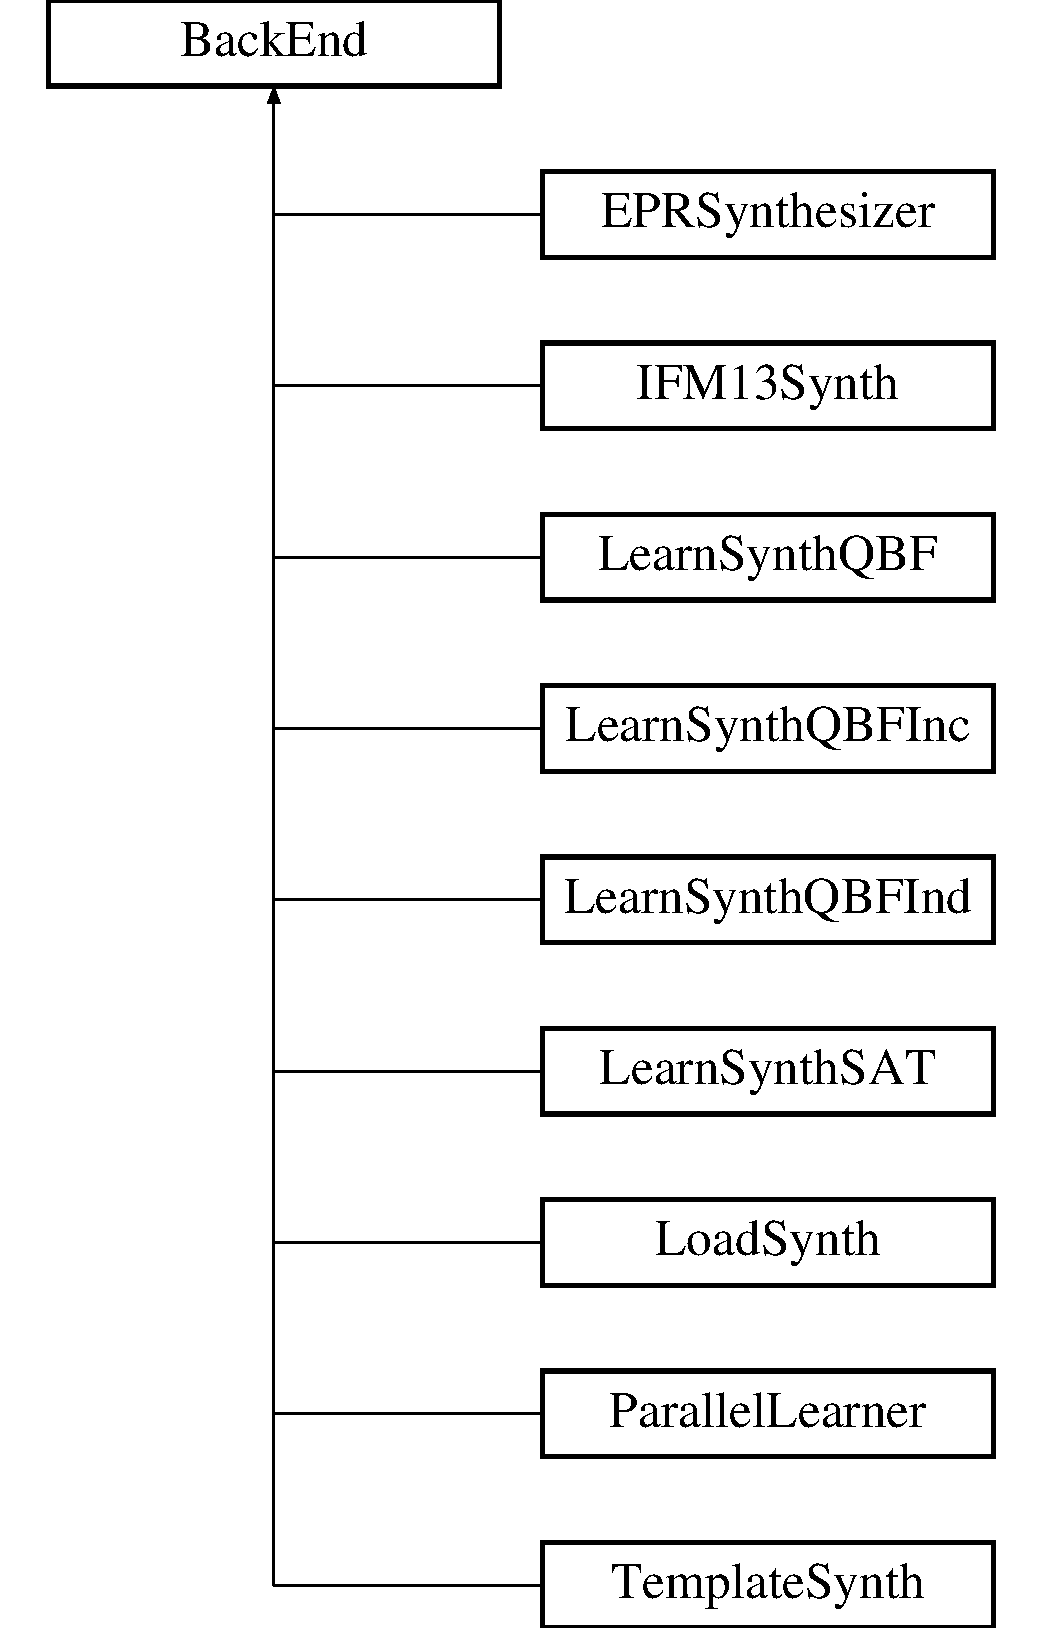
\includegraphics[height=10.000000cm]{classBackEnd}
\end{center}
\end{figure}
\subsection*{Public Member Functions}
\begin{DoxyCompactItemize}
\item 
\hyperlink{classBackEnd_afc7f71992574b71328373706917f2613}{Back\-End} ()
\begin{DoxyCompactList}\small\item\em Constructor. \end{DoxyCompactList}\item 
virtual \hyperlink{classBackEnd_ae54727f91644af02dc148eb820ae33c4}{$\sim$\-Back\-End} ()
\begin{DoxyCompactList}\small\item\em Constructor. \end{DoxyCompactList}\item 
virtual bool \hyperlink{classBackEnd_a099e717dc71e9cc2d838b1ca86340590}{run} ()=0
\begin{DoxyCompactList}\small\item\em Runs the \hyperlink{classBackEnd}{Back\-End}. \end{DoxyCompactList}\end{DoxyCompactItemize}
\subsection*{Private Member Functions}
\begin{DoxyCompactItemize}
\item 
\hyperlink{classBackEnd_a157822fdd45ad2cab86251e44ec6ad6b}{Back\-End} (const \hyperlink{classBackEnd}{Back\-End} \&other)
\begin{DoxyCompactList}\small\item\em Copy constructor. \end{DoxyCompactList}\item 
\hyperlink{classBackEnd}{Back\-End} \& \hyperlink{classBackEnd_a950f2ef881720fa8ffb90f7da23ab414}{operator=} (const \hyperlink{classBackEnd}{Back\-End} \&other)
\begin{DoxyCompactList}\small\item\em Assignment operator. \end{DoxyCompactList}\end{DoxyCompactItemize}


\subsection{Detailed Description}
An interface for the back-\/ends. 

This class provides an interface for all back-\/ends. Every back-\/end implements a different synthesis algorithm. This class is abstract, i.\-e., objects of this class cannot be instantiated. Instantiate one of the derived classes instead.

Many back-\/ends can be parameterized with a circuit extraction engine that extracts a circuit from the winning region once the winning region has been computed.

\begin{DoxyAuthor}{Author}
Robert Koenighofer (\href{mailto:robert.koenighofer@iaik.tugraz.at}{\tt robert.\-koenighofer@iaik.\-tugraz.\-at}) 
\end{DoxyAuthor}
\begin{DoxyVersion}{Version}
1.\-2.\-0 
\end{DoxyVersion}


Definition at line 49 of file Back\-End.\-h.



\subsection{Constructor \& Destructor Documentation}
\hypertarget{classBackEnd_afc7f71992574b71328373706917f2613}{\index{Back\-End@{Back\-End}!Back\-End@{Back\-End}}
\index{Back\-End@{Back\-End}!BackEnd@{Back\-End}}
\subsubsection[{Back\-End}]{\setlength{\rightskip}{0pt plus 5cm}Back\-End\-::\-Back\-End (
\begin{DoxyParamCaption}
{}
\end{DoxyParamCaption}
)}}\label{classBackEnd_afc7f71992574b71328373706917f2613}


Constructor. 



Definition at line 33 of file Back\-End.\-cpp.

\hypertarget{classBackEnd_ae54727f91644af02dc148eb820ae33c4}{\index{Back\-End@{Back\-End}!$\sim$\-Back\-End@{$\sim$\-Back\-End}}
\index{$\sim$\-Back\-End@{$\sim$\-Back\-End}!BackEnd@{Back\-End}}
\subsubsection[{$\sim$\-Back\-End}]{\setlength{\rightskip}{0pt plus 5cm}Back\-End\-::$\sim$\-Back\-End (
\begin{DoxyParamCaption}
{}
\end{DoxyParamCaption}
)\hspace{0.3cm}{\ttfamily [virtual]}}}\label{classBackEnd_ae54727f91644af02dc148eb820ae33c4}


Constructor. 



Definition at line 39 of file Back\-End.\-cpp.

\hypertarget{classBackEnd_a157822fdd45ad2cab86251e44ec6ad6b}{\index{Back\-End@{Back\-End}!Back\-End@{Back\-End}}
\index{Back\-End@{Back\-End}!BackEnd@{Back\-End}}
\subsubsection[{Back\-End}]{\setlength{\rightskip}{0pt plus 5cm}Back\-End\-::\-Back\-End (
\begin{DoxyParamCaption}
\item[{const {\bf Back\-End} \&}]{other}
\end{DoxyParamCaption}
)\hspace{0.3cm}{\ttfamily [private]}}}\label{classBackEnd_a157822fdd45ad2cab86251e44ec6ad6b}


Copy constructor. 

The copy constructor is disabled (set private) and not implemented.


\begin{DoxyParams}{Parameters}
{\em other} & The source for creating the copy. \\
\hline
\end{DoxyParams}


\subsection{Member Function Documentation}
\hypertarget{classBackEnd_a950f2ef881720fa8ffb90f7da23ab414}{\index{Back\-End@{Back\-End}!operator=@{operator=}}
\index{operator=@{operator=}!BackEnd@{Back\-End}}
\subsubsection[{operator=}]{\setlength{\rightskip}{0pt plus 5cm}{\bf Back\-End}\& Back\-End\-::operator= (
\begin{DoxyParamCaption}
\item[{const {\bf Back\-End} \&}]{other}
\end{DoxyParamCaption}
)\hspace{0.3cm}{\ttfamily [private]}}}\label{classBackEnd_a950f2ef881720fa8ffb90f7da23ab414}


Assignment operator. 

The assignment operator is disabled (set private) and not implemented.


\begin{DoxyParams}{Parameters}
{\em other} & The source for creating the copy. \\
\hline
\end{DoxyParams}
\begin{DoxyReturn}{Returns}
The result of the assignment, i.\-e, $\ast$this. 
\end{DoxyReturn}
\hypertarget{classBackEnd_a099e717dc71e9cc2d838b1ca86340590}{\index{Back\-End@{Back\-End}!run@{run}}
\index{run@{run}!BackEnd@{Back\-End}}
\subsubsection[{run}]{\setlength{\rightskip}{0pt plus 5cm}virtual bool Back\-End\-::run (
\begin{DoxyParamCaption}
{}
\end{DoxyParamCaption}
)\hspace{0.3cm}{\ttfamily [pure virtual]}}}\label{classBackEnd_a099e717dc71e9cc2d838b1ca86340590}


Runs the \hyperlink{classBackEnd}{Back\-End}. 

Every \hyperlink{classBackEnd}{Back\-End} implements a different synthesis algorithm. This method executes the synthesis algorithm. It expects that the specification has already been parsed (and is available in \hyperlink{classAIG2CNF}{A\-I\-G2\-C\-N\-F}).

This method is abstract, which means that it has to be implemented in the derived classes, i.\-e., in all classes actually implementing this interface.

\begin{DoxyReturn}{Returns}
True if the specification was realizable, false otherwise. 
\end{DoxyReturn}


Implemented in \hyperlink{classParallelLearner_a93acb74e7c8504d0ef2bd3697441b745}{Parallel\-Learner}, \hyperlink{classLearnSynthQBFInd_a6709343a109f82c427dcbc4a576d9c03}{Learn\-Synth\-Q\-B\-F\-Ind}, \hyperlink{classLearnSynthSAT_a13a50b2649f44d37761fdbff26e9c0c0}{Learn\-Synth\-S\-A\-T}, \hyperlink{classLearnSynthQBF_aed85bb2fe317a5fdc7eef71fe598c606}{Learn\-Synth\-Q\-B\-F}, \hyperlink{classIFM13Synth_a42adb4f76d88199d92b1bedb58a139f8}{I\-F\-M13\-Synth}, \hyperlink{classEPRSynthesizer_ab5eb613a7e5e4f8d408938531f745e4e}{E\-P\-R\-Synthesizer}, \hyperlink{classTemplateSynth_a5ad9855736c7d4dfdec08280d2424f80}{Template\-Synth}, \hyperlink{classLearnSynthQBFInc_af9563d1f3c657ed4730ee49e041bc300}{Learn\-Synth\-Q\-B\-F\-Inc}, and \hyperlink{classLoadSynth_a555ce9c74ad3143254f7a1d1cce094b0}{Load\-Synth}.



Referenced by main().



The documentation for this class was generated from the following files\-:\begin{DoxyCompactItemize}
\item 
src/\hyperlink{BackEnd_8h}{Back\-End.\-h}\item 
src/\hyperlink{BackEnd_8cpp}{Back\-End.\-cpp}\end{DoxyCompactItemize}

\hypertarget{classClauseExplorerSAT}{\section{Clause\-Explorer\-S\-A\-T Class Reference}
\label{classClauseExplorerSAT}\index{Clause\-Explorer\-S\-A\-T@{Clause\-Explorer\-S\-A\-T}}
}


Implements the method of \hyperlink{classLearnSynthSAT}{Learn\-Synth\-S\-A\-T} in a parallelized way.  




{\ttfamily \#include $<$Parallel\-Learner.\-h$>$}

\subsection*{Public Member Functions}
\begin{DoxyCompactItemize}
\item 
\hyperlink{classClauseExplorerSAT_afef2a28a6052b9d42de7d33736d53439}{Clause\-Explorer\-S\-A\-T} (size\-\_\-t instance\-\_\-nr, \hyperlink{classParallelLearner}{Parallel\-Learner} \&coordinator)
\begin{DoxyCompactList}\small\item\em Constructor if optimization R\-G is disabled. \end{DoxyCompactList}\item 
\hyperlink{classClauseExplorerSAT_aeb039a6f4bcccd7a899c22afbd2fd821}{Clause\-Explorer\-S\-A\-T} (size\-\_\-t instance\-\_\-nr, \hyperlink{classParallelLearner}{Parallel\-Learner} \&coordinator, const \hyperlink{classCNF}{C\-N\-F} \&prev\-\_\-trans\-\_\-or\-\_\-initial, const vector$<$ int $>$ \&current\-\_\-to\-\_\-previous\-\_\-map, int current\-\_\-state\-\_\-is\-\_\-initial)
\begin{DoxyCompactList}\small\item\em Constructor if optimization R\-G is enabled. \end{DoxyCompactList}\item 
virtual \hyperlink{classClauseExplorerSAT_aa5e321a156ef7fa6e21946594e500668}{$\sim$\-Clause\-Explorer\-S\-A\-T} ()
\begin{DoxyCompactList}\small\item\em Destructor. \end{DoxyCompactList}\item 
void \hyperlink{classClauseExplorerSAT_aae50270504a523ae79458c7eb1f2e9d1}{explore\-Clauses} ()
\begin{DoxyCompactList}\small\item\em The work-\/horse of this class. \end{DoxyCompactList}\item 
void \hyperlink{classClauseExplorerSAT_a36134b9b6f662c44de73e76146c256bd}{notify\-Before\-New\-Info} ()
\begin{DoxyCompactList}\small\item\em The method must be called before new information is passed to this object. \end{DoxyCompactList}\item 
void \hyperlink{classClauseExplorerSAT_a8289e4ba9921717f705a1b2fb2655761}{notify\-After\-New\-Info} ()
\begin{DoxyCompactList}\small\item\em The method must be called after new information is passed to this object. \end{DoxyCompactList}\item 
void \hyperlink{classClauseExplorerSAT_ad507ce2b3b33e0e5b27237fd24954d82}{notify\-New\-Win\-Reg\-Clause} (const vector$<$ int $>$ \&clause, int src)
\begin{DoxyCompactList}\small\item\em Notifies this worker about a new winning region clause. \end{DoxyCompactList}\item 
void \hyperlink{classClauseExplorerSAT_a1898760d3aec582ffbd0c5dc5460f8f9}{notify\-New\-Useless\-Input\-Clause} (const vector$<$ int $>$ \&clause, int level)
\begin{DoxyCompactList}\small\item\em Notifies this Clause\-Explorer\-S\-A\-T-\/instance that a new U-\/clause is available. \end{DoxyCompactList}\item 
void \hyperlink{classClauseExplorerSAT_ab08aedd836a12bdc325da6e3b0f8b711}{notify\-Restart} (const \hyperlink{classCNF}{C\-N\-F} \&restart\-\_\-with\-\_\-cnf)
\begin{DoxyCompactList}\small\item\em Notifies this Clause\-Explorer\-S\-A\-T-\/instance that it should restart its solver. \end{DoxyCompactList}\item 
const \hyperlink{classLearnStatisticsSAT}{Learn\-Statistics\-S\-A\-T} \& \hyperlink{classClauseExplorerSAT_a9798ab0d723cc896feef36e2fbf5311a}{get\-Statistics} () const 
\begin{DoxyCompactList}\small\item\em Returns the statistics and performance measures computed by this object. \end{DoxyCompactList}\end{DoxyCompactItemize}
\subsection*{Protected Member Functions}
\begin{DoxyCompactItemize}
\item 
void \hyperlink{classClauseExplorerSAT_aca3490db608f1c3a4a832e67654dd246}{consider\-New\-Info\-From\-Others} ()
\begin{DoxyCompactList}\small\item\em Considers new information discovered by other threads in the solvers. \end{DoxyCompactList}\item 
bool \hyperlink{classClauseExplorerSAT_a0515689c4464599e0d2d3c350d710d75}{wait\-Until\-Ongoing\-Restart\-Done} ()
\begin{DoxyCompactList}\small\item\em Checks if some other thread is computing a restart. If yes\-: waits until it is done. \end{DoxyCompactList}\item 
int \hyperlink{classClauseExplorerSAT_add20a0c539fdf734af6b0f49f2ba4ad9}{present\-To\-Previous} (int literal) const 
\begin{DoxyCompactList}\small\item\em Returns the previous-\/state copy of a literal. \end{DoxyCompactList}\item 
void \hyperlink{classClauseExplorerSAT_ae91fa23b183aa81824f16c3477643184}{present\-To\-Previous} (vector$<$ int $>$ \&cube\-\_\-or\-\_\-clause) const 
\begin{DoxyCompactList}\small\item\em Computes the previous-\/state copy of a cube or clause. \end{DoxyCompactList}\item 
void \hyperlink{classClauseExplorerSAT_a42355860aef189f2b89356ff347dab4d}{present\-To\-Previous} (\hyperlink{classCNF}{C\-N\-F} \&cnf) const 
\begin{DoxyCompactList}\small\item\em Computes the previous-\/state copy of a \hyperlink{classCNF}{C\-N\-F}. \end{DoxyCompactList}\end{DoxyCompactItemize}
\subsection*{Protected Attributes}
\begin{DoxyCompactItemize}
\item 
size\-\_\-t \hyperlink{classClauseExplorerSAT_ab9ff4163b38a8ce70e07b78ea2e76cc2}{instance\-\_\-nr\-\_\-}
\begin{DoxyCompactList}\small\item\em A unique instance number. \end{DoxyCompactList}\item 
bool \hyperlink{classClauseExplorerSAT_aca59e0b38c8a8fea9cf35d174969c41e}{use\-\_\-ind\-\_\-}
\begin{DoxyCompactList}\small\item\em A flag indicating if optimization R\-G should be used. \end{DoxyCompactList}\item 
\hyperlink{classLearnStatisticsSAT}{Learn\-Statistics\-S\-A\-T} \hyperlink{classClauseExplorerSAT_a1d37eb0233177911835bc073fbe1c224}{statistics\-\_\-}
\begin{DoxyCompactList}\small\item\em Stores and maintains statistics and performance measures. \end{DoxyCompactList}\item 
\hyperlink{classParallelLearner}{Parallel\-Learner} \& \hyperlink{classClauseExplorerSAT_a8909bb332c60d7611763ca5976fbe6f6}{coordinator\-\_\-}
\begin{DoxyCompactList}\small\item\em A reference to the coordinator. \end{DoxyCompactList}\item 
bool \hyperlink{classClauseExplorerSAT_a3edc259c6f39cce098ab18a2dce7f262}{precise\-\_\-}
\begin{DoxyCompactList}\small\item\em A flag indicating if the next-\/state copy of the winning region is accurate. \end{DoxyCompactList}\item 
\hyperlink{classSatSolver}{Sat\-Solver} $\ast$ \hyperlink{classClauseExplorerSAT_a65b5b3d04ff5be8bfec60d3dcf86e4d0}{solver\-\_\-i\-\_\-}
\begin{DoxyCompactList}\small\item\em The solver for computing counterexample-\/candidates. \end{DoxyCompactList}\item 
\hyperlink{classSatSolver}{Sat\-Solver} $\ast$ \hyperlink{classClauseExplorerSAT_a7884d171120e8397140e30fdc28767eb}{solver\-\_\-ctrl\-\_\-}
\begin{DoxyCompactList}\small\item\em The solver for checking counterexample-\/candidates. \end{DoxyCompactList}\item 
vector$<$ int $>$ \hyperlink{classClauseExplorerSAT_a9d9c6caf1a451ed22a096c2ef5e8bbc2}{vars\-\_\-to\-\_\-keep\-\_\-}
\begin{DoxyCompactList}\small\item\em A set of variables the solver should not optimize by the S\-A\-T-\/solver. \end{DoxyCompactList}\item 
mutex \hyperlink{classClauseExplorerSAT_a674651f8fbf9ed93264ce3369bd5332b}{new\-\_\-info\-\_\-lock\-\_\-}
\begin{DoxyCompactList}\small\item\em A lock to protect many fields from race conditions. \end{DoxyCompactList}\item 
\hyperlink{classCNF}{C\-N\-F} \hyperlink{classClauseExplorerSAT_a1a9dc7f76967c8164e9625df34dec172}{restart\-\_\-with\-\_\-cnf\-\_\-}
\begin{DoxyCompactList}\small\item\em A \hyperlink{classCNF}{C\-N\-F} to restart solver\-\_\-i\-\_\- with. \end{DoxyCompactList}\item 
\hyperlink{classCNF}{C\-N\-F} \hyperlink{classClauseExplorerSAT_a2c3e73b4c0529b9139354a965d34e81f}{new\-\_\-win\-\_\-reg\-\_\-clauses\-\_\-for\-\_\-solver\-\_\-i\-\_\-}
\begin{DoxyCompactList}\small\item\em All new winning region clauses that have not yet been fed into solver\-\_\-i\-\_\-. \end{DoxyCompactList}\item 
\hyperlink{classCNF}{C\-N\-F} \hyperlink{classClauseExplorerSAT_a7d923928f3cb6209b29f5cc5104b5fe2}{new\-\_\-win\-\_\-reg\-\_\-clauses\-\_\-for\-\_\-solver\-\_\-ctrl\-\_\-}
\begin{DoxyCompactList}\small\item\em All new winning region clauses that have not yet been fed into solver\-\_\-ctrl\-\_\-. \end{DoxyCompactList}\item 
\hyperlink{classCNF}{C\-N\-F} \hyperlink{classClauseExplorerSAT_a70c8edd590d75994ee354d591909cd35}{new\-\_\-foreign\-\_\-win\-\_\-reg\-\_\-clauses\-\_\-for\-\_\-solver\-\_\-i\-\_\-}
\begin{DoxyCompactList}\small\item\em All foreign winning region clauses that have not yet been fed into solver\-\_\-i\-\_\-. \end{DoxyCompactList}\item 
\hyperlink{classCNF}{C\-N\-F} \hyperlink{classClauseExplorerSAT_a3d1bdb9a6484c85af655a4eed1ee5f19}{new\-\_\-useless\-\_\-input\-\_\-clauses\-\_\-}
\begin{DoxyCompactList}\small\item\em All U-\/clauses that have not yet been added to \hyperlink{classClauseExplorerSAT_a65b5b3d04ff5be8bfec60d3dcf86e4d0}{solver\-\_\-i\-\_\-}. \end{DoxyCompactList}\item 
int \hyperlink{classClauseExplorerSAT_a67eeafbba9da9c87534f7ef26531a57a}{new\-\_\-useless\-\_\-input\-\_\-clauses\-\_\-level\-\_\-}
\begin{DoxyCompactList}\small\item\em The level on which the clauses in \hyperlink{classClauseExplorerSAT_a3d1bdb9a6484c85af655a4eed1ee5f19}{new\-\_\-useless\-\_\-input\-\_\-clauses\-\_\-} have been found. \end{DoxyCompactList}\item 
int \hyperlink{classClauseExplorerSAT_a0b5d716111026dd1cb4efe5855e2fe2f}{restart\-\_\-level\-\_\-}
\begin{DoxyCompactList}\small\item\em The number of solver restarts that have already been performed. \end{DoxyCompactList}\item 
int \hyperlink{classClauseExplorerSAT_adf9bfe4390d34e57e25f269afa1e7b25}{new\-\_\-restart\-\_\-level\-\_\-}
\begin{DoxyCompactList}\small\item\em The restart level we have after we consider \hyperlink{classClauseExplorerSAT_a1a9dc7f76967c8164e9625df34dec172}{restart\-\_\-with\-\_\-cnf\-\_\-}. \end{DoxyCompactList}\item 
\hyperlink{classSatSolver}{Sat\-Solver} $\ast$ \hyperlink{classClauseExplorerSAT_aba4c9ed8ccc28d89c094f3cd80157f3f}{solver\-\_\-ctrl\-\_\-ind\-\_\-}
\begin{DoxyCompactList}\small\item\em The solver for generalizing counterexamples if optimization R\-G is endabled. \end{DoxyCompactList}\item 
\hyperlink{classCNF}{C\-N\-F} \hyperlink{classClauseExplorerSAT_a445dd961b44b493e184ff42207132ea1}{prev\-\_\-trans\-\_\-or\-\_\-initial\-\_\-}
\begin{DoxyCompactList}\small\item\em Says\-: the current state is initial or the previous transition relation holds. \end{DoxyCompactList}\item 
vector$<$ int $>$ \hyperlink{classClauseExplorerSAT_aecf42678820d41d716fb23f833066da2}{current\-\_\-to\-\_\-previous\-\_\-map\-\_\-}
\begin{DoxyCompactList}\small\item\em A map from present-\/state variables to their previous-\/state copy. \end{DoxyCompactList}\item 
int \hyperlink{classClauseExplorerSAT_a210b4a062e0a949536b172d904a2219f}{current\-\_\-state\-\_\-is\-\_\-initial\-\_\-}
\begin{DoxyCompactList}\small\item\em Says\-: the current state is initial or the previous transition relation holds. \end{DoxyCompactList}\item 
int \hyperlink{classClauseExplorerSAT_ab98b3cf3447591b3e390e3d3a1d595e5}{prev\-\_\-safe\-\_\-}
\begin{DoxyCompactList}\small\item\em A literal saying that the previous-\/state is safe. \end{DoxyCompactList}\end{DoxyCompactItemize}
\subsection*{Private Member Functions}
\begin{DoxyCompactItemize}
\item 
\hyperlink{classClauseExplorerSAT_ad7a7e6be6d2450e716b2132308bdeeea}{Clause\-Explorer\-S\-A\-T} (const \hyperlink{classClauseExplorerSAT}{Clause\-Explorer\-S\-A\-T} \&other)
\begin{DoxyCompactList}\small\item\em Copy constructor. \end{DoxyCompactList}\item 
\hyperlink{classClauseExplorerSAT}{Clause\-Explorer\-S\-A\-T} \& \hyperlink{classClauseExplorerSAT_a1b2f9a77392cebd3e648d1696685e9b4}{operator=} (const \hyperlink{classClauseExplorerSAT}{Clause\-Explorer\-S\-A\-T} \&other)
\begin{DoxyCompactList}\small\item\em Assignment operator. \end{DoxyCompactList}\end{DoxyCompactItemize}


\subsection{Detailed Description}
Implements the method of \hyperlink{classLearnSynthSAT}{Learn\-Synth\-S\-A\-T} in a parallelized way. 

This class basically implements the same method as \hyperlink{classLearnSynthSAT}{Learn\-Synth\-S\-A\-T}. It only has a few additional methods to communicate with other threads. Whenever it finds a new clause of the winning region, it communicates this clause to all other worker-\/threads (via the \hyperlink{classParallelLearner}{Parallel\-Learner}, which acts as a coordinator). Also, if it finds out that some state-\/input combination is not useful for the antagonist in trying to leave the winning region, it communicates a clause to all other instances of the same class. For that to work, all Clause\-Explorer\-S\-A\-T-\/instances must be synchronized to a certain extend\-: All Clause\-Explorer\-S\-A\-T-\/instances must do solver restarts simultaneously, i.\-e., they must all work with the same next-\/state copy of the winning region. This is done by coordinating and communicating solver restarts via the \hyperlink{classParallelLearner}{Parallel\-Learner}.

\begin{DoxyAuthor}{Author}
Robert Koenighofer (\href{mailto:robert.koenighofer@iaik.tugraz.at}{\tt robert.\-koenighofer@iaik.\-tugraz.\-at}) 
\end{DoxyAuthor}
\begin{DoxyVersion}{Version}
1.\-0.\-0 
\end{DoxyVersion}


Definition at line 401 of file Parallel\-Learner.\-h.



\subsection{Constructor \& Destructor Documentation}
\hypertarget{classClauseExplorerSAT_afef2a28a6052b9d42de7d33736d53439}{\index{Clause\-Explorer\-S\-A\-T@{Clause\-Explorer\-S\-A\-T}!Clause\-Explorer\-S\-A\-T@{Clause\-Explorer\-S\-A\-T}}
\index{Clause\-Explorer\-S\-A\-T@{Clause\-Explorer\-S\-A\-T}!ClauseExplorerSAT@{Clause\-Explorer\-S\-A\-T}}
\subsubsection[{Clause\-Explorer\-S\-A\-T}]{\setlength{\rightskip}{0pt plus 5cm}Clause\-Explorer\-S\-A\-T\-::\-Clause\-Explorer\-S\-A\-T (
\begin{DoxyParamCaption}
\item[{size\-\_\-t}]{instance\-\_\-nr, }
\item[{{\bf Parallel\-Learner} \&}]{coordinator}
\end{DoxyParamCaption}
)}}\label{classClauseExplorerSAT_afef2a28a6052b9d42de7d33736d53439}


Constructor if optimization R\-G is disabled. 


\begin{DoxyParams}{Parameters}
{\em instance\-\_\-nr} & A unique instance number. It is used to bring in some asymmetry between the different Clause\-Explorer\-S\-A\-T-\/instances\-: depending on the instance number, the instance selects a different \hyperlink{classSatSolver}{Sat\-Solver} to use. \\
\hline
{\em coordinator} & A reference to the coordinator. All communication to other worker-\/threads is done via the coordinator. \\
\hline
\end{DoxyParams}


Definition at line 472 of file Parallel\-Learner.\-cpp.



References solver\-\_\-ctrl\-\_\-, and solver\-\_\-i\-\_\-.

\hypertarget{classClauseExplorerSAT_aeb039a6f4bcccd7a899c22afbd2fd821}{\index{Clause\-Explorer\-S\-A\-T@{Clause\-Explorer\-S\-A\-T}!Clause\-Explorer\-S\-A\-T@{Clause\-Explorer\-S\-A\-T}}
\index{Clause\-Explorer\-S\-A\-T@{Clause\-Explorer\-S\-A\-T}!ClauseExplorerSAT@{Clause\-Explorer\-S\-A\-T}}
\subsubsection[{Clause\-Explorer\-S\-A\-T}]{\setlength{\rightskip}{0pt plus 5cm}Clause\-Explorer\-S\-A\-T\-::\-Clause\-Explorer\-S\-A\-T (
\begin{DoxyParamCaption}
\item[{size\-\_\-t}]{instance\-\_\-nr, }
\item[{{\bf Parallel\-Learner} \&}]{coordinator, }
\item[{const {\bf C\-N\-F} \&}]{prev\-\_\-trans\-\_\-or\-\_\-initial, }
\item[{const vector$<$ int $>$ \&}]{current\-\_\-to\-\_\-previous\-\_\-map, }
\item[{int}]{current\-\_\-state\-\_\-is\-\_\-initial}
\end{DoxyParamCaption}
)}}\label{classClauseExplorerSAT_aeb039a6f4bcccd7a899c22afbd2fd821}


Constructor if optimization R\-G is enabled. 


\begin{DoxyParams}{Parameters}
{\em instance\-\_\-nr} & A unique instance number. It is used to bring in some asymmetry between the different Clause\-Explorer\-S\-A\-T-\/instances\-: depending on the instance number, the instance selects a different \hyperlink{classSatSolver}{Sat\-Solver} to use. \\
\hline
{\em coordinator} & A reference to the coordinator. All communication to other worker-\/threads is done via the coordinator. \\
\hline
{\em prev\-\_\-trans\-\_\-or\-\_\-initial} & A \hyperlink{classCNF}{C\-N\-F} that says\-: the current state is initial or the previous transition relation holds. This is an important building block for the \hyperlink{classCNF}{C\-N\-F} to generalize counterexamples if optimization R\-G is enabled. This \hyperlink{classCNF}{C\-N\-F} is computed only once by the \hyperlink{classParallelLearner}{Parallel\-Learner} and passed to all \hyperlink{classClauseExplorerSAT}{Clause\-Explorer\-S\-A\-T} instances. \\
\hline
{\em current\-\_\-to\-\_\-previous\-\_\-map} & A map from present-\/state variables to their previous-\/state copy. This map is computed only once by the \hyperlink{classParallelLearner}{Parallel\-Learner} and passed to all \hyperlink{classClauseExplorerSAT}{Clause\-Explorer\-S\-A\-T} instances. \\
\hline
{\em current\-\_\-state\-\_\-is\-\_\-initial} & A literal that is true if the current state is initial and false otherwise. The clauses assigning the literal are part of prev\-\_\-trans\-\_\-or\-\_\-initial. \\
\hline
\end{DoxyParams}


Definition at line 511 of file Parallel\-Learner.\-cpp.



References solver\-\_\-ctrl\-\_\-, solver\-\_\-ctrl\-\_\-ind\-\_\-, and solver\-\_\-i\-\_\-.

\hypertarget{classClauseExplorerSAT_aa5e321a156ef7fa6e21946594e500668}{\index{Clause\-Explorer\-S\-A\-T@{Clause\-Explorer\-S\-A\-T}!$\sim$\-Clause\-Explorer\-S\-A\-T@{$\sim$\-Clause\-Explorer\-S\-A\-T}}
\index{$\sim$\-Clause\-Explorer\-S\-A\-T@{$\sim$\-Clause\-Explorer\-S\-A\-T}!ClauseExplorerSAT@{Clause\-Explorer\-S\-A\-T}}
\subsubsection[{$\sim$\-Clause\-Explorer\-S\-A\-T}]{\setlength{\rightskip}{0pt plus 5cm}Clause\-Explorer\-S\-A\-T\-::$\sim$\-Clause\-Explorer\-S\-A\-T (
\begin{DoxyParamCaption}
{}
\end{DoxyParamCaption}
)\hspace{0.3cm}{\ttfamily [virtual]}}}\label{classClauseExplorerSAT_aa5e321a156ef7fa6e21946594e500668}


Destructor. 



Definition at line 567 of file Parallel\-Learner.\-cpp.



References solver\-\_\-ctrl\-\_\-, solver\-\_\-ctrl\-\_\-ind\-\_\-, and solver\-\_\-i\-\_\-.

\hypertarget{classClauseExplorerSAT_ad7a7e6be6d2450e716b2132308bdeeea}{\index{Clause\-Explorer\-S\-A\-T@{Clause\-Explorer\-S\-A\-T}!Clause\-Explorer\-S\-A\-T@{Clause\-Explorer\-S\-A\-T}}
\index{Clause\-Explorer\-S\-A\-T@{Clause\-Explorer\-S\-A\-T}!ClauseExplorerSAT@{Clause\-Explorer\-S\-A\-T}}
\subsubsection[{Clause\-Explorer\-S\-A\-T}]{\setlength{\rightskip}{0pt plus 5cm}Clause\-Explorer\-S\-A\-T\-::\-Clause\-Explorer\-S\-A\-T (
\begin{DoxyParamCaption}
\item[{const {\bf Clause\-Explorer\-S\-A\-T} \&}]{other}
\end{DoxyParamCaption}
)\hspace{0.3cm}{\ttfamily [private]}}}\label{classClauseExplorerSAT_ad7a7e6be6d2450e716b2132308bdeeea}


Copy constructor. 

The copy constructor is disabled (set private) and not implemented.


\begin{DoxyParams}{Parameters}
{\em other} & The source for creating the copy. \\
\hline
\end{DoxyParams}


\subsection{Member Function Documentation}
\hypertarget{classClauseExplorerSAT_aca3490db608f1c3a4a832e67654dd246}{\index{Clause\-Explorer\-S\-A\-T@{Clause\-Explorer\-S\-A\-T}!consider\-New\-Info\-From\-Others@{consider\-New\-Info\-From\-Others}}
\index{consider\-New\-Info\-From\-Others@{consider\-New\-Info\-From\-Others}!ClauseExplorerSAT@{Clause\-Explorer\-S\-A\-T}}
\subsubsection[{consider\-New\-Info\-From\-Others}]{\setlength{\rightskip}{0pt plus 5cm}void Clause\-Explorer\-S\-A\-T\-::consider\-New\-Info\-From\-Others (
\begin{DoxyParamCaption}
{}
\end{DoxyParamCaption}
)\hspace{0.3cm}{\ttfamily [protected]}}}\label{classClauseExplorerSAT_aca3490db608f1c3a4a832e67654dd246}


Considers new information discovered by other threads in the solvers. 

New information includes\-: 
\begin{DoxyItemize}
\item A new \hyperlink{classCNF}{C\-N\-F} for the solver to compute counterexamples (we need to do a restart). This info came from \hyperlink{classClauseExplorerSAT_ab08aedd836a12bdc325da6e3b0f8b711}{notify\-Restart()}. 
\item New clauses refining the winning region (coming from \hyperlink{classClauseExplorerSAT_ad507ce2b3b33e0e5b27237fd24954d82}{notify\-New\-Win\-Reg\-Clause()}). 
\item New clauses defining useless state-\/input combinations (coming from \hyperlink{classClauseExplorerSAT_a1898760d3aec582ffbd0c5dc5460f8f9}{notify\-New\-Useless\-Input\-Clause()}). 
\end{DoxyItemize}

Definition at line 773 of file Parallel\-Learner.\-cpp.



References C\-N\-F\-::clear(), C\-N\-F\-::get\-Nr\-Of\-Clauses(), Sat\-Solver\-::inc\-Add\-C\-N\-F(), new\-\_\-foreign\-\_\-win\-\_\-reg\-\_\-clauses\-\_\-for\-\_\-solver\-\_\-i\-\_\-, new\-\_\-info\-\_\-lock\-\_\-, new\-\_\-restart\-\_\-level\-\_\-, new\-\_\-useless\-\_\-input\-\_\-clauses\-\_\-, new\-\_\-useless\-\_\-input\-\_\-clauses\-\_\-level\-\_\-, new\-\_\-win\-\_\-reg\-\_\-clauses\-\_\-for\-\_\-solver\-\_\-ctrl\-\_\-, new\-\_\-win\-\_\-reg\-\_\-clauses\-\_\-for\-\_\-solver\-\_\-i\-\_\-, Learn\-Statistics\-S\-A\-T\-::notify\-Restart(), precise\-\_\-, present\-To\-Previous(), restart\-\_\-level\-\_\-, restart\-\_\-with\-\_\-cnf\-\_\-, solver\-\_\-ctrl\-\_\-, solver\-\_\-ctrl\-\_\-ind\-\_\-, solver\-\_\-i\-\_\-, Sat\-Solver\-::start\-Incremental\-Session(), statistics\-\_\-, C\-N\-F\-::swap\-Present\-To\-Next(), use\-\_\-ind\-\_\-, and vars\-\_\-to\-\_\-keep\-\_\-.



Referenced by explore\-Clauses().

\hypertarget{classClauseExplorerSAT_aae50270504a523ae79458c7eb1f2e9d1}{\index{Clause\-Explorer\-S\-A\-T@{Clause\-Explorer\-S\-A\-T}!explore\-Clauses@{explore\-Clauses}}
\index{explore\-Clauses@{explore\-Clauses}!ClauseExplorerSAT@{Clause\-Explorer\-S\-A\-T}}
\subsubsection[{explore\-Clauses}]{\setlength{\rightskip}{0pt plus 5cm}void Clause\-Explorer\-S\-A\-T\-::explore\-Clauses (
\begin{DoxyParamCaption}
{}
\end{DoxyParamCaption}
)}}\label{classClauseExplorerSAT_aae50270504a523ae79458c7eb1f2e9d1}


The work-\/horse of this class. 

This method computes clauses refining the winning region, just like \hyperlink{classLearnSynthSAT}{Learn\-Synth\-S\-A\-T}. It only has a few additional methods to communicate with other threads. Whenever it finds a new clause of the winning region, it communicates it to all other worker-\/threads (via the \hyperlink{classParallelLearner}{Parallel\-Learner}, which acts as a coordinator). Also, if it finds out that some state-\/input combination is not useful for the antagonist in trying to leave the winning region, it communicates a clause to all other instances of the same class. In every iteration, it also considers all new incoming clauses found by others. All Clause\-Explorer\-S\-A\-T-\/instances must be synchronized to a certain extend\-: All Clause\-Explorer\-S\-A\-T-\/instances must do solver restarts simultaneously, i.\-e., they must all work with the same next-\/state copy of the winning region. This is done by coordinating and communicating solver restarts via the \hyperlink{classParallelLearner}{Parallel\-Learner}. 

Definition at line 578 of file Parallel\-Learner.\-cpp.



References consider\-New\-Info\-From\-Others(), Utils\-::contains\-Init(), coordinator\-\_\-, Var\-Info\-::\-C\-T\-R\-L, current\-\_\-state\-\_\-is\-\_\-initial\-\_\-, E\-X\-P\-L, Utils\-::extract(), A\-I\-G2\-C\-N\-F\-::get\-Next\-Safe\-States(), A\-I\-G2\-C\-N\-F\-::get\-Next\-Unsafe\-States(), A\-I\-G2\-C\-N\-F\-::get\-Safe\-States(), A\-I\-G2\-C\-N\-F\-::get\-Trans(), Var\-Manager\-::get\-Vars\-Of\-Type(), Sat\-Solver\-::inc\-Add\-C\-N\-F(), Sat\-Solver\-::inc\-Add\-Cube(), Sat\-Solver\-::inc\-Add\-Neg\-Cube\-As\-Clause(), Sat\-Solver\-::inc\-Add\-Unit\-Clause(), Sat\-Solver\-::inc\-Is\-Sat(), Sat\-Solver\-::inc\-Is\-Sat\-Model\-Or\-Core(), Sat\-Solver\-::inc\-Pop(), Sat\-Solver\-::inc\-Push(), Var\-Info\-::\-I\-N\-P\-U\-T, Var\-Manager\-::instance(), A\-I\-G2\-C\-N\-F\-::instance(), instance\-\_\-nr\-\_\-, L\-\_\-\-D\-B\-G, M\-A\-S\-S\-E\-R\-T, Learn\-Statistics\-S\-A\-T\-::notify\-After\-Check\-Candidate\-Failed(), Learn\-Statistics\-S\-A\-T\-::notify\-After\-Check\-Candidate\-Found(), Learn\-Statistics\-S\-A\-T\-::notify\-After\-Compute\-Candidate(), Learn\-Statistics\-S\-A\-T\-::notify\-After\-Refine(), Learn\-Statistics\-S\-A\-T\-::notify\-Before\-Check\-Candidate(), Learn\-Statistics\-S\-A\-T\-::notify\-Before\-Compute\-Candidate(), Learn\-Statistics\-S\-A\-T\-::notify\-Before\-Refine(), Parallel\-Learner\-::notify\-New\-Counterexample(), Parallel\-Learner\-::notify\-New\-Useless\-Input\-Clause(), Parallel\-Learner\-::notify\-New\-Win\-Reg\-Clause(), precise\-\_\-, Var\-Info\-::\-P\-R\-E\-S\-\_\-\-S\-T\-A\-T\-E, present\-To\-Previous(), prev\-\_\-safe\-\_\-, prev\-\_\-trans\-\_\-or\-\_\-initial\-\_\-, Utils\-::randomize(), R\-E\-A\-L\-I\-Z\-A\-B\-L\-E, Utils\-::remove(), restart\-\_\-level\-\_\-, Parallel\-Learner\-::result\-\_\-, solver\-\_\-ctrl\-\_\-, solver\-\_\-ctrl\-\_\-ind\-\_\-, solver\-\_\-i\-\_\-, Sat\-Solver\-::start\-Incremental\-Session(), statistics\-\_\-, Utils\-::swap\-Present\-To\-Next(), Parallel\-Learner\-::trigger\-Explorer\-Restart(), U\-N\-K\-N\-O\-W\-N, U\-N\-R\-E\-A\-L\-I\-Z\-A\-B\-L\-E, use\-\_\-ind\-\_\-, vars\-\_\-to\-\_\-keep\-\_\-, and wait\-Until\-Ongoing\-Restart\-Done().



Referenced by Parallel\-Learner\-::run().

\hypertarget{classClauseExplorerSAT_a9798ab0d723cc896feef36e2fbf5311a}{\index{Clause\-Explorer\-S\-A\-T@{Clause\-Explorer\-S\-A\-T}!get\-Statistics@{get\-Statistics}}
\index{get\-Statistics@{get\-Statistics}!ClauseExplorerSAT@{Clause\-Explorer\-S\-A\-T}}
\subsubsection[{get\-Statistics}]{\setlength{\rightskip}{0pt plus 5cm}const {\bf Learn\-Statistics\-S\-A\-T} \& Clause\-Explorer\-S\-A\-T\-::get\-Statistics (
\begin{DoxyParamCaption}
{}
\end{DoxyParamCaption}
) const}}\label{classClauseExplorerSAT_a9798ab0d723cc896feef36e2fbf5311a}


Returns the statistics and performance measures computed by this object. 

It is used by the \hyperlink{classParallelLearner}{Parallel\-Learner} to merge the statistics of the different workers.

\begin{DoxyReturn}{Returns}
The statistics and performance measures computed by this object. 
\end{DoxyReturn}


Definition at line 767 of file Parallel\-Learner.\-cpp.



References statistics\-\_\-.

\hypertarget{classClauseExplorerSAT_a8289e4ba9921717f705a1b2fb2655761}{\index{Clause\-Explorer\-S\-A\-T@{Clause\-Explorer\-S\-A\-T}!notify\-After\-New\-Info@{notify\-After\-New\-Info}}
\index{notify\-After\-New\-Info@{notify\-After\-New\-Info}!ClauseExplorerSAT@{Clause\-Explorer\-S\-A\-T}}
\subsubsection[{notify\-After\-New\-Info}]{\setlength{\rightskip}{0pt plus 5cm}void Clause\-Explorer\-S\-A\-T\-::notify\-After\-New\-Info (
\begin{DoxyParamCaption}
{}
\end{DoxyParamCaption}
)}}\label{classClauseExplorerSAT_a8289e4ba9921717f705a1b2fb2655761}


The method must be called after new information is passed to this object. 

See \hyperlink{classClauseExplorerSAT_a36134b9b6f662c44de73e76146c256bd}{notify\-Before\-New\-Info()} for an explanation. 

Definition at line 724 of file Parallel\-Learner.\-cpp.



References new\-\_\-info\-\_\-lock\-\_\-.

\hypertarget{classClauseExplorerSAT_a36134b9b6f662c44de73e76146c256bd}{\index{Clause\-Explorer\-S\-A\-T@{Clause\-Explorer\-S\-A\-T}!notify\-Before\-New\-Info@{notify\-Before\-New\-Info}}
\index{notify\-Before\-New\-Info@{notify\-Before\-New\-Info}!ClauseExplorerSAT@{Clause\-Explorer\-S\-A\-T}}
\subsubsection[{notify\-Before\-New\-Info}]{\setlength{\rightskip}{0pt plus 5cm}void Clause\-Explorer\-S\-A\-T\-::notify\-Before\-New\-Info (
\begin{DoxyParamCaption}
{}
\end{DoxyParamCaption}
)}}\label{classClauseExplorerSAT_a36134b9b6f662c44de73e76146c256bd}


The method must be called before new information is passed to this object. 

After the new information has been set, \hyperlink{classClauseExplorerSAT_a8289e4ba9921717f705a1b2fb2655761}{notify\-After\-New\-Info()} must be called. This way the coordinator (the \hyperlink{classParallelLearner}{Parallel\-Learner}) can inform all Clause\-Explorer\-S\-A\-T-\/instances simultaneously\-: It calls \hyperlink{classClauseExplorerSAT_a36134b9b6f662c44de73e76146c256bd}{notify\-Before\-New\-Info()} on all instances, then communicates the new information to all instances, then calls \hyperlink{classClauseExplorerSAT_a8289e4ba9921717f705a1b2fb2655761}{notify\-After\-New\-Info()} on all instances. This way, no thread can work with the new information before the others got it. This method must be used for \hyperlink{classClauseExplorerSAT_ad507ce2b3b33e0e5b27237fd24954d82}{notify\-New\-Win\-Reg\-Clause()}, \hyperlink{classClauseExplorerSAT_a1898760d3aec582ffbd0c5dc5460f8f9}{notify\-New\-Useless\-Input\-Clause()}, and \hyperlink{classClauseExplorerSAT_a1898760d3aec582ffbd0c5dc5460f8f9}{notify\-New\-Useless\-Input\-Clause()}. If this method finds out that the specification is realizable or unrealizable, it sets the flag \hyperlink{classParallelLearner_a757f8817809cce5c0408cdc41d6db1b8}{Parallel\-Learner\-::result\-\_\-} accordingly. It also polls this flag regularly. If it has been set by some other thread, it quits. 

Definition at line 718 of file Parallel\-Learner.\-cpp.



References new\-\_\-info\-\_\-lock\-\_\-.

\hypertarget{classClauseExplorerSAT_a1898760d3aec582ffbd0c5dc5460f8f9}{\index{Clause\-Explorer\-S\-A\-T@{Clause\-Explorer\-S\-A\-T}!notify\-New\-Useless\-Input\-Clause@{notify\-New\-Useless\-Input\-Clause}}
\index{notify\-New\-Useless\-Input\-Clause@{notify\-New\-Useless\-Input\-Clause}!ClauseExplorerSAT@{Clause\-Explorer\-S\-A\-T}}
\subsubsection[{notify\-New\-Useless\-Input\-Clause}]{\setlength{\rightskip}{0pt plus 5cm}void Clause\-Explorer\-S\-A\-T\-::notify\-New\-Useless\-Input\-Clause (
\begin{DoxyParamCaption}
\item[{const vector$<$ int $>$ \&}]{clause, }
\item[{int}]{level}
\end{DoxyParamCaption}
)}}\label{classClauseExplorerSAT_a1898760d3aec582ffbd0c5dc5460f8f9}


Notifies this Clause\-Explorer\-S\-A\-T-\/instance that a new U-\/clause is available. 

A U-\/clause states that a certain state-\/input is useless for the antagonist in trying to leave the winning region (see \hyperlink{classLearnSynthSAT}{Learn\-Synth\-S\-A\-T} for details). If one \hyperlink{classClauseExplorerSAT}{Clause\-Explorer\-S\-A\-T} discovers such a clause, it communicates it to all other Clause\-Explorer\-S\-A\-T-\/instances such that they can also benefit from it and do not need to re-\/discover the same fact again.

\begin{DoxyNote}{Note}
Be sure to call \hyperlink{classClauseExplorerSAT_a36134b9b6f662c44de73e76146c256bd}{notify\-Before\-New\-Info()} before this method and \hyperlink{classClauseExplorerSAT_a8289e4ba9921717f705a1b2fb2655761}{notify\-After\-New\-Info()} after calling this method. 
\end{DoxyNote}

\begin{DoxyParams}{Parameters}
{\em clause} & A new U-\/clause stating that a certain state-\/input is useless for the antagonist in trying to leave the winning region (see \hyperlink{classLearnSynthSAT}{Learn\-Synth\-S\-A\-T} for details). \\
\hline
{\em level} & The restart level (the number of solver restarts that have already been performed. This information allows this instance to decide whether or not this clause is useful for her (or if it is already out-\/dated). \\
\hline
\end{DoxyParams}


Definition at line 745 of file Parallel\-Learner.\-cpp.



References C\-N\-F\-::add\-Clause(), C\-N\-F\-::clear(), new\-\_\-useless\-\_\-input\-\_\-clauses\-\_\-, and new\-\_\-useless\-\_\-input\-\_\-clauses\-\_\-level\-\_\-.

\hypertarget{classClauseExplorerSAT_ad507ce2b3b33e0e5b27237fd24954d82}{\index{Clause\-Explorer\-S\-A\-T@{Clause\-Explorer\-S\-A\-T}!notify\-New\-Win\-Reg\-Clause@{notify\-New\-Win\-Reg\-Clause}}
\index{notify\-New\-Win\-Reg\-Clause@{notify\-New\-Win\-Reg\-Clause}!ClauseExplorerSAT@{Clause\-Explorer\-S\-A\-T}}
\subsubsection[{notify\-New\-Win\-Reg\-Clause}]{\setlength{\rightskip}{0pt plus 5cm}void Clause\-Explorer\-S\-A\-T\-::notify\-New\-Win\-Reg\-Clause (
\begin{DoxyParamCaption}
\item[{const vector$<$ int $>$ \&}]{clause, }
\item[{int}]{src}
\end{DoxyParamCaption}
)}}\label{classClauseExplorerSAT_ad507ce2b3b33e0e5b27237fd24954d82}


Notifies this worker about a new winning region clause. 

\begin{DoxyNote}{Note}
Be sure to call \hyperlink{classClauseExplorerSAT_a36134b9b6f662c44de73e76146c256bd}{notify\-Before\-New\-Info()} before this method and \hyperlink{classClauseExplorerSAT_a8289e4ba9921717f705a1b2fb2655761}{notify\-After\-New\-Info()} after calling this method. 
\end{DoxyNote}

\begin{DoxyParams}{Parameters}
{\em clause} & The new clause that has been discovered. \\
\hline
{\em src} & An integer number defining which kind of worker-\/thread discovered the clause. For performance reasons, this method distinguishes between clauses discovered by Clause\-Explorer\-S\-A\-T-\/instances, and clauses discovered by other kinds of workers. \\
\hline
\end{DoxyParams}


Definition at line 730 of file Parallel\-Learner.\-cpp.



References C\-N\-F\-::add\-Clause(), E\-X\-P\-L, new\-\_\-foreign\-\_\-win\-\_\-reg\-\_\-clauses\-\_\-for\-\_\-solver\-\_\-i\-\_\-, new\-\_\-win\-\_\-reg\-\_\-clauses\-\_\-for\-\_\-solver\-\_\-ctrl\-\_\-, and new\-\_\-win\-\_\-reg\-\_\-clauses\-\_\-for\-\_\-solver\-\_\-i\-\_\-.

\hypertarget{classClauseExplorerSAT_ab08aedd836a12bdc325da6e3b0f8b711}{\index{Clause\-Explorer\-S\-A\-T@{Clause\-Explorer\-S\-A\-T}!notify\-Restart@{notify\-Restart}}
\index{notify\-Restart@{notify\-Restart}!ClauseExplorerSAT@{Clause\-Explorer\-S\-A\-T}}
\subsubsection[{notify\-Restart}]{\setlength{\rightskip}{0pt plus 5cm}void Clause\-Explorer\-S\-A\-T\-::notify\-Restart (
\begin{DoxyParamCaption}
\item[{const {\bf C\-N\-F} \&}]{restart\-\_\-with\-\_\-cnf}
\end{DoxyParamCaption}
)}}\label{classClauseExplorerSAT_ab08aedd836a12bdc325da6e3b0f8b711}


Notifies this Clause\-Explorer\-S\-A\-T-\/instance that it should restart its solver. 

The \hyperlink{classClauseExplorerSAT}{Clause\-Explorer\-S\-A\-T} update their next-\/state copy of the winning region only in a lazy manner. This allows them to use incremental S\-A\-T-\/solving more effectively. See \hyperlink{classLearnSynthSAT}{Learn\-Synth\-S\-A\-T} for a description. If no more solutions exists with one next-\/state copy of the winning region, it must be updated to the newest version. This method tells this instance that such a newer version should be used.

It is absolutely important that all \hyperlink{classClauseExplorerSAT}{Clause\-Explorer\-S\-A\-T} instances work with the same next-\/state copy of the winning region. Otherwise, they could not exchange U-\/clauses (or rather, the U-\/clause discovered by one thread would not make sense for the other).

\begin{DoxySeeAlso}{See Also}
\hyperlink{classClauseExplorerSAT_a1898760d3aec582ffbd0c5dc5460f8f9}{notify\-New\-Useless\-Input\-Clause()} 

\hyperlink{classParallelLearner_a2b8e4330afb7e99c19d2d7da15c30cc3}{Parallel\-Learner\-::trigger\-Explorer\-Restart()} 
\end{DoxySeeAlso}

\begin{DoxyParams}{Parameters}
{\em restart\-\_\-with\-\_\-cnf} & The \hyperlink{classCNF}{C\-N\-F} for W \& T \& !\-W', where W is the current over-\/approximation of the winning region. \\
\hline
\end{DoxyParams}


Definition at line 757 of file Parallel\-Learner.\-cpp.



References C\-N\-F\-::clear(), new\-\_\-foreign\-\_\-win\-\_\-reg\-\_\-clauses\-\_\-for\-\_\-solver\-\_\-i\-\_\-, new\-\_\-restart\-\_\-level\-\_\-, new\-\_\-win\-\_\-reg\-\_\-clauses\-\_\-for\-\_\-solver\-\_\-i\-\_\-, and restart\-\_\-with\-\_\-cnf\-\_\-.

\hypertarget{classClauseExplorerSAT_a1b2f9a77392cebd3e648d1696685e9b4}{\index{Clause\-Explorer\-S\-A\-T@{Clause\-Explorer\-S\-A\-T}!operator=@{operator=}}
\index{operator=@{operator=}!ClauseExplorerSAT@{Clause\-Explorer\-S\-A\-T}}
\subsubsection[{operator=}]{\setlength{\rightskip}{0pt plus 5cm}{\bf Clause\-Explorer\-S\-A\-T}\& Clause\-Explorer\-S\-A\-T\-::operator= (
\begin{DoxyParamCaption}
\item[{const {\bf Clause\-Explorer\-S\-A\-T} \&}]{other}
\end{DoxyParamCaption}
)\hspace{0.3cm}{\ttfamily [private]}}}\label{classClauseExplorerSAT_a1b2f9a77392cebd3e648d1696685e9b4}


Assignment operator. 

The assignment operator is disabled (set private) and not implemented.


\begin{DoxyParams}{Parameters}
{\em other} & The source for creating the copy. \\
\hline
\end{DoxyParams}
\begin{DoxyReturn}{Returns}
The result of the assignment, i.\-e, $\ast$this. 
\end{DoxyReturn}
\hypertarget{classClauseExplorerSAT_add20a0c539fdf734af6b0f49f2ba4ad9}{\index{Clause\-Explorer\-S\-A\-T@{Clause\-Explorer\-S\-A\-T}!present\-To\-Previous@{present\-To\-Previous}}
\index{present\-To\-Previous@{present\-To\-Previous}!ClauseExplorerSAT@{Clause\-Explorer\-S\-A\-T}}
\subsubsection[{present\-To\-Previous}]{\setlength{\rightskip}{0pt plus 5cm}int Clause\-Explorer\-S\-A\-T\-::present\-To\-Previous (
\begin{DoxyParamCaption}
\item[{int}]{literal}
\end{DoxyParamCaption}
) const\hspace{0.3cm}{\ttfamily [protected]}}}\label{classClauseExplorerSAT_add20a0c539fdf734af6b0f49f2ba4ad9}


Returns the previous-\/state copy of a literal. 


\begin{DoxyParams}{Parameters}
{\em literal} & The literal to transform. \\
\hline
\end{DoxyParams}
\begin{DoxyReturn}{Returns}
The previous-\/state copy of a literal. 
\end{DoxyReturn}


Definition at line 841 of file Parallel\-Learner.\-cpp.



References current\-\_\-to\-\_\-previous\-\_\-map\-\_\-.



Referenced by consider\-New\-Info\-From\-Others(), explore\-Clauses(), and present\-To\-Previous().

\hypertarget{classClauseExplorerSAT_ae91fa23b183aa81824f16c3477643184}{\index{Clause\-Explorer\-S\-A\-T@{Clause\-Explorer\-S\-A\-T}!present\-To\-Previous@{present\-To\-Previous}}
\index{present\-To\-Previous@{present\-To\-Previous}!ClauseExplorerSAT@{Clause\-Explorer\-S\-A\-T}}
\subsubsection[{present\-To\-Previous}]{\setlength{\rightskip}{0pt plus 5cm}void Clause\-Explorer\-S\-A\-T\-::present\-To\-Previous (
\begin{DoxyParamCaption}
\item[{vector$<$ int $>$ \&}]{cube\-\_\-or\-\_\-clause}
\end{DoxyParamCaption}
) const\hspace{0.3cm}{\ttfamily [protected]}}}\label{classClauseExplorerSAT_ae91fa23b183aa81824f16c3477643184}


Computes the previous-\/state copy of a cube or clause. 


\begin{DoxyParams}{Parameters}
{\em cube\-\_\-or\-\_\-clause} & A cube or clause (in form of a vector of literals) over the present state variables. This vector is overwritten by the corresponding cube of clause over the previous-\/state literals (i.\-e., all literals are replaced by their previous-\/state copy). \\
\hline
\end{DoxyParams}


Definition at line 851 of file Parallel\-Learner.\-cpp.



References present\-To\-Previous().

\hypertarget{classClauseExplorerSAT_a42355860aef189f2b89356ff347dab4d}{\index{Clause\-Explorer\-S\-A\-T@{Clause\-Explorer\-S\-A\-T}!present\-To\-Previous@{present\-To\-Previous}}
\index{present\-To\-Previous@{present\-To\-Previous}!ClauseExplorerSAT@{Clause\-Explorer\-S\-A\-T}}
\subsubsection[{present\-To\-Previous}]{\setlength{\rightskip}{0pt plus 5cm}void Clause\-Explorer\-S\-A\-T\-::present\-To\-Previous (
\begin{DoxyParamCaption}
\item[{{\bf C\-N\-F} \&}]{cnf}
\end{DoxyParamCaption}
) const\hspace{0.3cm}{\ttfamily [protected]}}}\label{classClauseExplorerSAT_a42355860aef189f2b89356ff347dab4d}


Computes the previous-\/state copy of a \hyperlink{classCNF}{C\-N\-F}. 


\begin{DoxyParams}{Parameters}
{\em cnf} & A \hyperlink{classCNF}{C\-N\-F} formula over the present state variables. This \hyperlink{classCNF}{C\-N\-F} is overwritten by the corresponding \hyperlink{classCNF}{C\-N\-F} over the previous-\/state literals (i.\-e., all literals are replaced by their previous-\/state copy). \\
\hline
\end{DoxyParams}


Definition at line 858 of file Parallel\-Learner.\-cpp.



References C\-N\-F\-::add\-Clause(), C\-N\-F\-::clear(), C\-N\-F\-::get\-Clauses(), and present\-To\-Previous().

\hypertarget{classClauseExplorerSAT_a0515689c4464599e0d2d3c350d710d75}{\index{Clause\-Explorer\-S\-A\-T@{Clause\-Explorer\-S\-A\-T}!wait\-Until\-Ongoing\-Restart\-Done@{wait\-Until\-Ongoing\-Restart\-Done}}
\index{wait\-Until\-Ongoing\-Restart\-Done@{wait\-Until\-Ongoing\-Restart\-Done}!ClauseExplorerSAT@{Clause\-Explorer\-S\-A\-T}}
\subsubsection[{wait\-Until\-Ongoing\-Restart\-Done}]{\setlength{\rightskip}{0pt plus 5cm}bool Clause\-Explorer\-S\-A\-T\-::wait\-Until\-Ongoing\-Restart\-Done (
\begin{DoxyParamCaption}
{}
\end{DoxyParamCaption}
)\hspace{0.3cm}{\ttfamily [protected]}}}\label{classClauseExplorerSAT_a0515689c4464599e0d2d3c350d710d75}


Checks if some other thread is computing a restart. If yes\-: waits until it is done. 

This is just a performance optimization. Before we trigger a restart, we check if someone else is already working on a restart (computing a restart point takes some time because we also compress the \hyperlink{classCNF}{C\-N\-F} of the winning region for performance reasons). If so, we wait until it is done. Otherwise, we would do two very similar restarts one after the other. This would be correct, but more inefficient.

\begin{DoxyReturn}{Returns}
True if a restart is available. False otherwise. 
\end{DoxyReturn}


Definition at line 827 of file Parallel\-Learner.\-cpp.



References coordinator\-\_\-, C\-N\-F\-::get\-Nr\-Of\-Clauses(), new\-\_\-info\-\_\-lock\-\_\-, restart\-\_\-with\-\_\-cnf\-\_\-, and Parallel\-Learner\-::var\-\_\-man\-\_\-lock\-\_\-.



Referenced by explore\-Clauses().



\subsection{Member Data Documentation}
\hypertarget{classClauseExplorerSAT_a8909bb332c60d7611763ca5976fbe6f6}{\index{Clause\-Explorer\-S\-A\-T@{Clause\-Explorer\-S\-A\-T}!coordinator\-\_\-@{coordinator\-\_\-}}
\index{coordinator\-\_\-@{coordinator\-\_\-}!ClauseExplorerSAT@{Clause\-Explorer\-S\-A\-T}}
\subsubsection[{coordinator\-\_\-}]{\setlength{\rightskip}{0pt plus 5cm}{\bf Parallel\-Learner}\& Clause\-Explorer\-S\-A\-T\-::coordinator\-\_\-\hspace{0.3cm}{\ttfamily [protected]}}}\label{classClauseExplorerSAT_a8909bb332c60d7611763ca5976fbe6f6}


A reference to the coordinator. 

All communication to other worker-\/threads is done via the coordinator. 

Definition at line 634 of file Parallel\-Learner.\-h.



Referenced by explore\-Clauses(), and wait\-Until\-Ongoing\-Restart\-Done().

\hypertarget{classClauseExplorerSAT_a210b4a062e0a949536b172d904a2219f}{\index{Clause\-Explorer\-S\-A\-T@{Clause\-Explorer\-S\-A\-T}!current\-\_\-state\-\_\-is\-\_\-initial\-\_\-@{current\-\_\-state\-\_\-is\-\_\-initial\-\_\-}}
\index{current\-\_\-state\-\_\-is\-\_\-initial\-\_\-@{current\-\_\-state\-\_\-is\-\_\-initial\-\_\-}!ClauseExplorerSAT@{Clause\-Explorer\-S\-A\-T}}
\subsubsection[{current\-\_\-state\-\_\-is\-\_\-initial\-\_\-}]{\setlength{\rightskip}{0pt plus 5cm}int Clause\-Explorer\-S\-A\-T\-::current\-\_\-state\-\_\-is\-\_\-initial\-\_\-\hspace{0.3cm}{\ttfamily [protected]}}}\label{classClauseExplorerSAT_a210b4a062e0a949536b172d904a2219f}


Says\-: the current state is initial or the previous transition relation holds. 

This \hyperlink{classCNF}{C\-N\-F} expresses that the current state is initial or the previous-\/state copy of the transition relation holds. This is an important building block for the \hyperlink{classCNF}{C\-N\-F} to generalize counterexamples if optimization R\-G is enabled. If optimization R\-G is disabled, then this field is meaningless. 

Definition at line 787 of file Parallel\-Learner.\-h.



Referenced by explore\-Clauses().

\hypertarget{classClauseExplorerSAT_aecf42678820d41d716fb23f833066da2}{\index{Clause\-Explorer\-S\-A\-T@{Clause\-Explorer\-S\-A\-T}!current\-\_\-to\-\_\-previous\-\_\-map\-\_\-@{current\-\_\-to\-\_\-previous\-\_\-map\-\_\-}}
\index{current\-\_\-to\-\_\-previous\-\_\-map\-\_\-@{current\-\_\-to\-\_\-previous\-\_\-map\-\_\-}!ClauseExplorerSAT@{Clause\-Explorer\-S\-A\-T}}
\subsubsection[{current\-\_\-to\-\_\-previous\-\_\-map\-\_\-}]{\setlength{\rightskip}{0pt plus 5cm}vector$<$int$>$ Clause\-Explorer\-S\-A\-T\-::current\-\_\-to\-\_\-previous\-\_\-map\-\_\-\hspace{0.3cm}{\ttfamily [protected]}}}\label{classClauseExplorerSAT_aecf42678820d41d716fb23f833066da2}


A map from present-\/state variables to their previous-\/state copy. 

If optimization R\-G is disabled, then this \hyperlink{classCNF}{C\-N\-F} is empty. 

Definition at line 776 of file Parallel\-Learner.\-h.



Referenced by present\-To\-Previous().

\hypertarget{classClauseExplorerSAT_ab9ff4163b38a8ce70e07b78ea2e76cc2}{\index{Clause\-Explorer\-S\-A\-T@{Clause\-Explorer\-S\-A\-T}!instance\-\_\-nr\-\_\-@{instance\-\_\-nr\-\_\-}}
\index{instance\-\_\-nr\-\_\-@{instance\-\_\-nr\-\_\-}!ClauseExplorerSAT@{Clause\-Explorer\-S\-A\-T}}
\subsubsection[{instance\-\_\-nr\-\_\-}]{\setlength{\rightskip}{0pt plus 5cm}size\-\_\-t Clause\-Explorer\-S\-A\-T\-::instance\-\_\-nr\-\_\-\hspace{0.3cm}{\ttfamily [protected]}}}\label{classClauseExplorerSAT_ab9ff4163b38a8ce70e07b78ea2e76cc2}


A unique instance number. 

It is used to bring in some asymmetry between the different Clause\-Explorer\-S\-A\-T-\/instances\-: depending on the instance number, the instance selects a different \hyperlink{classSatSolver}{Sat\-Solver} to use. Furthermore, it is used for debugging to print more meaningful messages (W\-H\-O is printing a message). 

Definition at line 613 of file Parallel\-Learner.\-h.



Referenced by explore\-Clauses().

\hypertarget{classClauseExplorerSAT_a70c8edd590d75994ee354d591909cd35}{\index{Clause\-Explorer\-S\-A\-T@{Clause\-Explorer\-S\-A\-T}!new\-\_\-foreign\-\_\-win\-\_\-reg\-\_\-clauses\-\_\-for\-\_\-solver\-\_\-i\-\_\-@{new\-\_\-foreign\-\_\-win\-\_\-reg\-\_\-clauses\-\_\-for\-\_\-solver\-\_\-i\-\_\-}}
\index{new\-\_\-foreign\-\_\-win\-\_\-reg\-\_\-clauses\-\_\-for\-\_\-solver\-\_\-i\-\_\-@{new\-\_\-foreign\-\_\-win\-\_\-reg\-\_\-clauses\-\_\-for\-\_\-solver\-\_\-i\-\_\-}!ClauseExplorerSAT@{Clause\-Explorer\-S\-A\-T}}
\subsubsection[{new\-\_\-foreign\-\_\-win\-\_\-reg\-\_\-clauses\-\_\-for\-\_\-solver\-\_\-i\-\_\-}]{\setlength{\rightskip}{0pt plus 5cm}{\bf C\-N\-F} Clause\-Explorer\-S\-A\-T\-::new\-\_\-foreign\-\_\-win\-\_\-reg\-\_\-clauses\-\_\-for\-\_\-solver\-\_\-i\-\_\-\hspace{0.3cm}{\ttfamily [protected]}}}\label{classClauseExplorerSAT_a70c8edd590d75994ee354d591909cd35}


All foreign winning region clauses that have not yet been fed into solver\-\_\-i\-\_\-. 

This \hyperlink{classCNF}{C\-N\-F} contains only clauses that have not been discovered by Clause\-Explorer\-S\-A\-T-\/threads. Clauses discovered by Clause\-Explorer\-S\-A\-T-\/threads are stored in \hyperlink{classClauseExplorerSAT_a2c3e73b4c0529b9139354a965d34e81f}{new\-\_\-win\-\_\-reg\-\_\-clauses\-\_\-for\-\_\-solver\-\_\-i\-\_\-}. Clauses discovered by other threads are handled in a special way for performance reasons. They are not added immediately because this could make the solver imprecise, which prevents it from terminating. Foreign clauses are only added if the \hyperlink{classClauseExplorerSAT_a65b5b3d04ff5be8bfec60d3dcf86e4d0}{solver\-\_\-i\-\_\-} is already imprecise (precise\-\_\- is false). Otherwise, other threads could spam Clause\-Explorer\-S\-A\-T-\/threads with clauses that prevent the Clause\-Explorer\-S\-A\-T-\/threads from being precise long enough to conclude realizability. (Acutally I don't know if this is really an issue, but the optimization is implemented just in case). 

Definition at line 722 of file Parallel\-Learner.\-h.



Referenced by consider\-New\-Info\-From\-Others(), notify\-New\-Win\-Reg\-Clause(), and notify\-Restart().

\hypertarget{classClauseExplorerSAT_a674651f8fbf9ed93264ce3369bd5332b}{\index{Clause\-Explorer\-S\-A\-T@{Clause\-Explorer\-S\-A\-T}!new\-\_\-info\-\_\-lock\-\_\-@{new\-\_\-info\-\_\-lock\-\_\-}}
\index{new\-\_\-info\-\_\-lock\-\_\-@{new\-\_\-info\-\_\-lock\-\_\-}!ClauseExplorerSAT@{Clause\-Explorer\-S\-A\-T}}
\subsubsection[{new\-\_\-info\-\_\-lock\-\_\-}]{\setlength{\rightskip}{0pt plus 5cm}mutex Clause\-Explorer\-S\-A\-T\-::new\-\_\-info\-\_\-lock\-\_\-\hspace{0.3cm}{\ttfamily [protected]}}}\label{classClauseExplorerSAT_a674651f8fbf9ed93264ce3369bd5332b}


A lock to protect many fields from race conditions. 

This lock protects the fields 
\begin{DoxyItemize}
\item \hyperlink{classClauseExplorerSAT_a1a9dc7f76967c8164e9625df34dec172}{restart\-\_\-with\-\_\-cnf\-\_\-} 
\item \hyperlink{classClauseExplorerSAT_a2c3e73b4c0529b9139354a965d34e81f}{new\-\_\-win\-\_\-reg\-\_\-clauses\-\_\-for\-\_\-solver\-\_\-i\-\_\-} 
\item \hyperlink{classClauseExplorerSAT_a7d923928f3cb6209b29f5cc5104b5fe2}{new\-\_\-win\-\_\-reg\-\_\-clauses\-\_\-for\-\_\-solver\-\_\-ctrl\-\_\-} 
\item \hyperlink{classClauseExplorerSAT_a70c8edd590d75994ee354d591909cd35}{new\-\_\-foreign\-\_\-win\-\_\-reg\-\_\-clauses\-\_\-for\-\_\-solver\-\_\-i\-\_\-} 
\item \hyperlink{classClauseExplorerSAT_a3d1bdb9a6484c85af655a4eed1ee5f19}{new\-\_\-useless\-\_\-input\-\_\-clauses\-\_\-} 
\item \hyperlink{classClauseExplorerSAT_a67eeafbba9da9c87534f7ef26531a57a}{new\-\_\-useless\-\_\-input\-\_\-clauses\-\_\-level\-\_\-} 
\end{DoxyItemize}From race conditions. These fields are modified by other threads when new information comes in. They are read by this thread when this new information is taken into account.

\begin{DoxyRefDesc}{Todo}
\item[\hyperlink{todo__todo000008}{Todo}]A more fine-\/grained locking could improve the performance. \end{DoxyRefDesc}


Definition at line 679 of file Parallel\-Learner.\-h.



Referenced by consider\-New\-Info\-From\-Others(), notify\-After\-New\-Info(), notify\-Before\-New\-Info(), and wait\-Until\-Ongoing\-Restart\-Done().

\hypertarget{classClauseExplorerSAT_adf9bfe4390d34e57e25f269afa1e7b25}{\index{Clause\-Explorer\-S\-A\-T@{Clause\-Explorer\-S\-A\-T}!new\-\_\-restart\-\_\-level\-\_\-@{new\-\_\-restart\-\_\-level\-\_\-}}
\index{new\-\_\-restart\-\_\-level\-\_\-@{new\-\_\-restart\-\_\-level\-\_\-}!ClauseExplorerSAT@{Clause\-Explorer\-S\-A\-T}}
\subsubsection[{new\-\_\-restart\-\_\-level\-\_\-}]{\setlength{\rightskip}{0pt plus 5cm}int Clause\-Explorer\-S\-A\-T\-::new\-\_\-restart\-\_\-level\-\_\-\hspace{0.3cm}{\ttfamily [protected]}}}\label{classClauseExplorerSAT_adf9bfe4390d34e57e25f269afa1e7b25}


The restart level we have after we consider \hyperlink{classClauseExplorerSAT_a1a9dc7f76967c8164e9625df34dec172}{restart\-\_\-with\-\_\-cnf\-\_\-}. 

The thing is\-: this thread can skip a restart level completely if it does not get scheduled often. In this case, we have to increase our restart level by more than one when we actually do the restart (consider \hyperlink{classClauseExplorerSAT_a1a9dc7f76967c8164e9625df34dec172}{restart\-\_\-with\-\_\-cnf\-\_\-}). The new restart level is tracked by this field. 

Definition at line 754 of file Parallel\-Learner.\-h.



Referenced by consider\-New\-Info\-From\-Others(), and notify\-Restart().

\hypertarget{classClauseExplorerSAT_a3d1bdb9a6484c85af655a4eed1ee5f19}{\index{Clause\-Explorer\-S\-A\-T@{Clause\-Explorer\-S\-A\-T}!new\-\_\-useless\-\_\-input\-\_\-clauses\-\_\-@{new\-\_\-useless\-\_\-input\-\_\-clauses\-\_\-}}
\index{new\-\_\-useless\-\_\-input\-\_\-clauses\-\_\-@{new\-\_\-useless\-\_\-input\-\_\-clauses\-\_\-}!ClauseExplorerSAT@{Clause\-Explorer\-S\-A\-T}}
\subsubsection[{new\-\_\-useless\-\_\-input\-\_\-clauses\-\_\-}]{\setlength{\rightskip}{0pt plus 5cm}{\bf C\-N\-F} Clause\-Explorer\-S\-A\-T\-::new\-\_\-useless\-\_\-input\-\_\-clauses\-\_\-\hspace{0.3cm}{\ttfamily [protected]}}}\label{classClauseExplorerSAT_a3d1bdb9a6484c85af655a4eed1ee5f19}


All U-\/clauses that have not yet been added to \hyperlink{classClauseExplorerSAT_a65b5b3d04ff5be8bfec60d3dcf86e4d0}{solver\-\_\-i\-\_\-}. 

A U-\/clause states that a certain state-\/input is useless for the antagonist in trying to leave the winning region (see \hyperlink{classLearnSynthSAT}{Learn\-Synth\-S\-A\-T} for details). 

Definition at line 730 of file Parallel\-Learner.\-h.



Referenced by consider\-New\-Info\-From\-Others(), and notify\-New\-Useless\-Input\-Clause().

\hypertarget{classClauseExplorerSAT_a67eeafbba9da9c87534f7ef26531a57a}{\index{Clause\-Explorer\-S\-A\-T@{Clause\-Explorer\-S\-A\-T}!new\-\_\-useless\-\_\-input\-\_\-clauses\-\_\-level\-\_\-@{new\-\_\-useless\-\_\-input\-\_\-clauses\-\_\-level\-\_\-}}
\index{new\-\_\-useless\-\_\-input\-\_\-clauses\-\_\-level\-\_\-@{new\-\_\-useless\-\_\-input\-\_\-clauses\-\_\-level\-\_\-}!ClauseExplorerSAT@{Clause\-Explorer\-S\-A\-T}}
\subsubsection[{new\-\_\-useless\-\_\-input\-\_\-clauses\-\_\-level\-\_\-}]{\setlength{\rightskip}{0pt plus 5cm}int Clause\-Explorer\-S\-A\-T\-::new\-\_\-useless\-\_\-input\-\_\-clauses\-\_\-level\-\_\-\hspace{0.3cm}{\ttfamily [protected]}}}\label{classClauseExplorerSAT_a67eeafbba9da9c87534f7ef26531a57a}


The level on which the clauses in \hyperlink{classClauseExplorerSAT_a3d1bdb9a6484c85af655a4eed1ee5f19}{new\-\_\-useless\-\_\-input\-\_\-clauses\-\_\-} have been found. 

'Level' means the number of solver restarts that have already been performed. \hyperlink{classClauseExplorerSAT_a3d1bdb9a6484c85af655a4eed1ee5f19}{new\-\_\-useless\-\_\-input\-\_\-clauses\-\_\-} are only considered if their level matches the \hyperlink{classClauseExplorerSAT_a0b5d716111026dd1cb4efe5855e2fe2f}{restart\-\_\-level\-\_\-} of this object. 

Definition at line 739 of file Parallel\-Learner.\-h.



Referenced by consider\-New\-Info\-From\-Others(), and notify\-New\-Useless\-Input\-Clause().

\hypertarget{classClauseExplorerSAT_a7d923928f3cb6209b29f5cc5104b5fe2}{\index{Clause\-Explorer\-S\-A\-T@{Clause\-Explorer\-S\-A\-T}!new\-\_\-win\-\_\-reg\-\_\-clauses\-\_\-for\-\_\-solver\-\_\-ctrl\-\_\-@{new\-\_\-win\-\_\-reg\-\_\-clauses\-\_\-for\-\_\-solver\-\_\-ctrl\-\_\-}}
\index{new\-\_\-win\-\_\-reg\-\_\-clauses\-\_\-for\-\_\-solver\-\_\-ctrl\-\_\-@{new\-\_\-win\-\_\-reg\-\_\-clauses\-\_\-for\-\_\-solver\-\_\-ctrl\-\_\-}!ClauseExplorerSAT@{Clause\-Explorer\-S\-A\-T}}
\subsubsection[{new\-\_\-win\-\_\-reg\-\_\-clauses\-\_\-for\-\_\-solver\-\_\-ctrl\-\_\-}]{\setlength{\rightskip}{0pt plus 5cm}{\bf C\-N\-F} Clause\-Explorer\-S\-A\-T\-::new\-\_\-win\-\_\-reg\-\_\-clauses\-\_\-for\-\_\-solver\-\_\-ctrl\-\_\-\hspace{0.3cm}{\ttfamily [protected]}}}\label{classClauseExplorerSAT_a7d923928f3cb6209b29f5cc5104b5fe2}


All new winning region clauses that have not yet been fed into solver\-\_\-ctrl\-\_\-. 

We do not distinguish clauses discovered by Clause\-Explorer\-S\-A\-T-\/threads and clauses discovered by other threads. We also add all clauses to solver\-\_\-ctrl\-\_\- immediately. 

Definition at line 706 of file Parallel\-Learner.\-h.



Referenced by consider\-New\-Info\-From\-Others(), and notify\-New\-Win\-Reg\-Clause().

\hypertarget{classClauseExplorerSAT_a2c3e73b4c0529b9139354a965d34e81f}{\index{Clause\-Explorer\-S\-A\-T@{Clause\-Explorer\-S\-A\-T}!new\-\_\-win\-\_\-reg\-\_\-clauses\-\_\-for\-\_\-solver\-\_\-i\-\_\-@{new\-\_\-win\-\_\-reg\-\_\-clauses\-\_\-for\-\_\-solver\-\_\-i\-\_\-}}
\index{new\-\_\-win\-\_\-reg\-\_\-clauses\-\_\-for\-\_\-solver\-\_\-i\-\_\-@{new\-\_\-win\-\_\-reg\-\_\-clauses\-\_\-for\-\_\-solver\-\_\-i\-\_\-}!ClauseExplorerSAT@{Clause\-Explorer\-S\-A\-T}}
\subsubsection[{new\-\_\-win\-\_\-reg\-\_\-clauses\-\_\-for\-\_\-solver\-\_\-i\-\_\-}]{\setlength{\rightskip}{0pt plus 5cm}{\bf C\-N\-F} Clause\-Explorer\-S\-A\-T\-::new\-\_\-win\-\_\-reg\-\_\-clauses\-\_\-for\-\_\-solver\-\_\-i\-\_\-\hspace{0.3cm}{\ttfamily [protected]}}}\label{classClauseExplorerSAT_a2c3e73b4c0529b9139354a965d34e81f}


All new winning region clauses that have not yet been fed into solver\-\_\-i\-\_\-. 

This \hyperlink{classCNF}{C\-N\-F} contains only clauses that have been discovered by Clause\-Explorer\-S\-A\-T-\/threads. Clauses discovered by other threads are stored in \hyperlink{classClauseExplorerSAT_a70c8edd590d75994ee354d591909cd35}{new\-\_\-foreign\-\_\-win\-\_\-reg\-\_\-clauses\-\_\-for\-\_\-solver\-\_\-i\-\_\-} because they are treaded specially (for performance reasons). 

Definition at line 698 of file Parallel\-Learner.\-h.



Referenced by consider\-New\-Info\-From\-Others(), notify\-New\-Win\-Reg\-Clause(), and notify\-Restart().

\hypertarget{classClauseExplorerSAT_a3edc259c6f39cce098ab18a2dce7f262}{\index{Clause\-Explorer\-S\-A\-T@{Clause\-Explorer\-S\-A\-T}!precise\-\_\-@{precise\-\_\-}}
\index{precise\-\_\-@{precise\-\_\-}!ClauseExplorerSAT@{Clause\-Explorer\-S\-A\-T}}
\subsubsection[{precise\-\_\-}]{\setlength{\rightskip}{0pt plus 5cm}bool Clause\-Explorer\-S\-A\-T\-::precise\-\_\-\hspace{0.3cm}{\ttfamily [protected]}}}\label{classClauseExplorerSAT_a3edc259c6f39cce098ab18a2dce7f262}


A flag indicating if the next-\/state copy of the winning region is accurate. 

\begin{DoxySeeAlso}{See Also}
\hyperlink{classLearnSynthSAT}{Learn\-Synth\-S\-A\-T} 
\end{DoxySeeAlso}


Definition at line 641 of file Parallel\-Learner.\-h.



Referenced by consider\-New\-Info\-From\-Others(), and explore\-Clauses().

\hypertarget{classClauseExplorerSAT_ab98b3cf3447591b3e390e3d3a1d595e5}{\index{Clause\-Explorer\-S\-A\-T@{Clause\-Explorer\-S\-A\-T}!prev\-\_\-safe\-\_\-@{prev\-\_\-safe\-\_\-}}
\index{prev\-\_\-safe\-\_\-@{prev\-\_\-safe\-\_\-}!ClauseExplorerSAT@{Clause\-Explorer\-S\-A\-T}}
\subsubsection[{prev\-\_\-safe\-\_\-}]{\setlength{\rightskip}{0pt plus 5cm}int Clause\-Explorer\-S\-A\-T\-::prev\-\_\-safe\-\_\-\hspace{0.3cm}{\ttfamily [protected]}}}\label{classClauseExplorerSAT_ab98b3cf3447591b3e390e3d3a1d595e5}


A literal saying that the previous-\/state is safe. 

We store this literal here and do not read it out of the \hyperlink{classVarManager}{Var\-Manager} again and again to avoid a concurrency issue. The \hyperlink{classVarManager}{Var\-Manager} is sometimes modified (new temporary variables are created). This does not affect the literal defining safe states. However, we do not want to lock reading-\/accesses to the variable manager and we do not want to read out the variable manager in an inconsistent state. Hence, we read it out once and store it. If optimization R\-G is disabled, then this field is meaningless. 

Definition at line 799 of file Parallel\-Learner.\-h.



Referenced by explore\-Clauses().

\hypertarget{classClauseExplorerSAT_a445dd961b44b493e184ff42207132ea1}{\index{Clause\-Explorer\-S\-A\-T@{Clause\-Explorer\-S\-A\-T}!prev\-\_\-trans\-\_\-or\-\_\-initial\-\_\-@{prev\-\_\-trans\-\_\-or\-\_\-initial\-\_\-}}
\index{prev\-\_\-trans\-\_\-or\-\_\-initial\-\_\-@{prev\-\_\-trans\-\_\-or\-\_\-initial\-\_\-}!ClauseExplorerSAT@{Clause\-Explorer\-S\-A\-T}}
\subsubsection[{prev\-\_\-trans\-\_\-or\-\_\-initial\-\_\-}]{\setlength{\rightskip}{0pt plus 5cm}{\bf C\-N\-F} Clause\-Explorer\-S\-A\-T\-::prev\-\_\-trans\-\_\-or\-\_\-initial\-\_\-\hspace{0.3cm}{\ttfamily [protected]}}}\label{classClauseExplorerSAT_a445dd961b44b493e184ff42207132ea1}


Says\-: the current state is initial or the previous transition relation holds. 

This \hyperlink{classCNF}{C\-N\-F} expresses that the current state is initial or the previous-\/state copy of the transition relation holds. This is an important building block for the \hyperlink{classCNF}{C\-N\-F} to generalize counterexamples if optimization R\-G is enabled. If optimization R\-G is disabled, then this \hyperlink{classCNF}{C\-N\-F} is empty. 

Definition at line 769 of file Parallel\-Learner.\-h.



Referenced by explore\-Clauses().

\hypertarget{classClauseExplorerSAT_a0b5d716111026dd1cb4efe5855e2fe2f}{\index{Clause\-Explorer\-S\-A\-T@{Clause\-Explorer\-S\-A\-T}!restart\-\_\-level\-\_\-@{restart\-\_\-level\-\_\-}}
\index{restart\-\_\-level\-\_\-@{restart\-\_\-level\-\_\-}!ClauseExplorerSAT@{Clause\-Explorer\-S\-A\-T}}
\subsubsection[{restart\-\_\-level\-\_\-}]{\setlength{\rightskip}{0pt plus 5cm}int Clause\-Explorer\-S\-A\-T\-::restart\-\_\-level\-\_\-\hspace{0.3cm}{\ttfamily [protected]}}}\label{classClauseExplorerSAT_a0b5d716111026dd1cb4efe5855e2fe2f}


The number of solver restarts that have already been performed. 



Definition at line 744 of file Parallel\-Learner.\-h.



Referenced by consider\-New\-Info\-From\-Others(), and explore\-Clauses().

\hypertarget{classClauseExplorerSAT_a1a9dc7f76967c8164e9625df34dec172}{\index{Clause\-Explorer\-S\-A\-T@{Clause\-Explorer\-S\-A\-T}!restart\-\_\-with\-\_\-cnf\-\_\-@{restart\-\_\-with\-\_\-cnf\-\_\-}}
\index{restart\-\_\-with\-\_\-cnf\-\_\-@{restart\-\_\-with\-\_\-cnf\-\_\-}!ClauseExplorerSAT@{Clause\-Explorer\-S\-A\-T}}
\subsubsection[{restart\-\_\-with\-\_\-cnf\-\_\-}]{\setlength{\rightskip}{0pt plus 5cm}{\bf C\-N\-F} Clause\-Explorer\-S\-A\-T\-::restart\-\_\-with\-\_\-cnf\-\_\-\hspace{0.3cm}{\ttfamily [protected]}}}\label{classClauseExplorerSAT_a1a9dc7f76967c8164e9625df34dec172}


A \hyperlink{classCNF}{C\-N\-F} to restart solver\-\_\-i\-\_\- with. 

This \hyperlink{classCNF}{C\-N\-F} contains F \& T \& !\-F', where F is the current over-\/approximation of the winning region if a restart of solver\-\_\-i\-\_\- needs to be done. If no restart needs to be done, then this \hyperlink{classCNF}{C\-N\-F} is empty (i.\-e., true). 

Definition at line 688 of file Parallel\-Learner.\-h.



Referenced by consider\-New\-Info\-From\-Others(), notify\-Restart(), and wait\-Until\-Ongoing\-Restart\-Done().

\hypertarget{classClauseExplorerSAT_a7884d171120e8397140e30fdc28767eb}{\index{Clause\-Explorer\-S\-A\-T@{Clause\-Explorer\-S\-A\-T}!solver\-\_\-ctrl\-\_\-@{solver\-\_\-ctrl\-\_\-}}
\index{solver\-\_\-ctrl\-\_\-@{solver\-\_\-ctrl\-\_\-}!ClauseExplorerSAT@{Clause\-Explorer\-S\-A\-T}}
\subsubsection[{solver\-\_\-ctrl\-\_\-}]{\setlength{\rightskip}{0pt plus 5cm}{\bf Sat\-Solver}$\ast$ Clause\-Explorer\-S\-A\-T\-::solver\-\_\-ctrl\-\_\-\hspace{0.3cm}{\ttfamily [protected]}}}\label{classClauseExplorerSAT_a7884d171120e8397140e30fdc28767eb}


The solver for checking counterexample-\/candidates. 

It is also used to generalize counterexamples if optimization R\-G is disabled. 

Definition at line 653 of file Parallel\-Learner.\-h.



Referenced by Clause\-Explorer\-S\-A\-T(), consider\-New\-Info\-From\-Others(), explore\-Clauses(), and $\sim$\-Clause\-Explorer\-S\-A\-T().

\hypertarget{classClauseExplorerSAT_aba4c9ed8ccc28d89c094f3cd80157f3f}{\index{Clause\-Explorer\-S\-A\-T@{Clause\-Explorer\-S\-A\-T}!solver\-\_\-ctrl\-\_\-ind\-\_\-@{solver\-\_\-ctrl\-\_\-ind\-\_\-}}
\index{solver\-\_\-ctrl\-\_\-ind\-\_\-@{solver\-\_\-ctrl\-\_\-ind\-\_\-}!ClauseExplorerSAT@{Clause\-Explorer\-S\-A\-T}}
\subsubsection[{solver\-\_\-ctrl\-\_\-ind\-\_\-}]{\setlength{\rightskip}{0pt plus 5cm}{\bf Sat\-Solver}$\ast$ Clause\-Explorer\-S\-A\-T\-::solver\-\_\-ctrl\-\_\-ind\-\_\-\hspace{0.3cm}{\ttfamily [protected]}}}\label{classClauseExplorerSAT_aba4c9ed8ccc28d89c094f3cd80157f3f}


The solver for generalizing counterexamples if optimization R\-G is endabled. 



Definition at line 759 of file Parallel\-Learner.\-h.



Referenced by Clause\-Explorer\-S\-A\-T(), consider\-New\-Info\-From\-Others(), explore\-Clauses(), and $\sim$\-Clause\-Explorer\-S\-A\-T().

\hypertarget{classClauseExplorerSAT_a65b5b3d04ff5be8bfec60d3dcf86e4d0}{\index{Clause\-Explorer\-S\-A\-T@{Clause\-Explorer\-S\-A\-T}!solver\-\_\-i\-\_\-@{solver\-\_\-i\-\_\-}}
\index{solver\-\_\-i\-\_\-@{solver\-\_\-i\-\_\-}!ClauseExplorerSAT@{Clause\-Explorer\-S\-A\-T}}
\subsubsection[{solver\-\_\-i\-\_\-}]{\setlength{\rightskip}{0pt plus 5cm}{\bf Sat\-Solver}$\ast$ Clause\-Explorer\-S\-A\-T\-::solver\-\_\-i\-\_\-\hspace{0.3cm}{\ttfamily [protected]}}}\label{classClauseExplorerSAT_a65b5b3d04ff5be8bfec60d3dcf86e4d0}


The solver for computing counterexample-\/candidates. 



Definition at line 646 of file Parallel\-Learner.\-h.



Referenced by Clause\-Explorer\-S\-A\-T(), consider\-New\-Info\-From\-Others(), explore\-Clauses(), and $\sim$\-Clause\-Explorer\-S\-A\-T().

\hypertarget{classClauseExplorerSAT_a1d37eb0233177911835bc073fbe1c224}{\index{Clause\-Explorer\-S\-A\-T@{Clause\-Explorer\-S\-A\-T}!statistics\-\_\-@{statistics\-\_\-}}
\index{statistics\-\_\-@{statistics\-\_\-}!ClauseExplorerSAT@{Clause\-Explorer\-S\-A\-T}}
\subsubsection[{statistics\-\_\-}]{\setlength{\rightskip}{0pt plus 5cm}{\bf Learn\-Statistics\-S\-A\-T} Clause\-Explorer\-S\-A\-T\-::statistics\-\_\-\hspace{0.3cm}{\ttfamily [protected]}}}\label{classClauseExplorerSAT_a1d37eb0233177911835bc073fbe1c224}


Stores and maintains statistics and performance measures. 

Basically, this is a merge of the statistics from all worker-\/threads. 

Definition at line 627 of file Parallel\-Learner.\-h.



Referenced by consider\-New\-Info\-From\-Others(), explore\-Clauses(), and get\-Statistics().

\hypertarget{classClauseExplorerSAT_aca59e0b38c8a8fea9cf35d174969c41e}{\index{Clause\-Explorer\-S\-A\-T@{Clause\-Explorer\-S\-A\-T}!use\-\_\-ind\-\_\-@{use\-\_\-ind\-\_\-}}
\index{use\-\_\-ind\-\_\-@{use\-\_\-ind\-\_\-}!ClauseExplorerSAT@{Clause\-Explorer\-S\-A\-T}}
\subsubsection[{use\-\_\-ind\-\_\-}]{\setlength{\rightskip}{0pt plus 5cm}bool Clause\-Explorer\-S\-A\-T\-::use\-\_\-ind\-\_\-\hspace{0.3cm}{\ttfamily [protected]}}}\label{classClauseExplorerSAT_aca59e0b38c8a8fea9cf35d174969c41e}


A flag indicating if optimization R\-G should be used. 

See \hyperlink{classLearnSynthQBFInd}{Learn\-Synth\-Q\-B\-F\-Ind} for an explanation. 

Definition at line 620 of file Parallel\-Learner.\-h.



Referenced by consider\-New\-Info\-From\-Others(), and explore\-Clauses().

\hypertarget{classClauseExplorerSAT_a9d9c6caf1a451ed22a096c2ef5e8bbc2}{\index{Clause\-Explorer\-S\-A\-T@{Clause\-Explorer\-S\-A\-T}!vars\-\_\-to\-\_\-keep\-\_\-@{vars\-\_\-to\-\_\-keep\-\_\-}}
\index{vars\-\_\-to\-\_\-keep\-\_\-@{vars\-\_\-to\-\_\-keep\-\_\-}!ClauseExplorerSAT@{Clause\-Explorer\-S\-A\-T}}
\subsubsection[{vars\-\_\-to\-\_\-keep\-\_\-}]{\setlength{\rightskip}{0pt plus 5cm}vector$<$int$>$ Clause\-Explorer\-S\-A\-T\-::vars\-\_\-to\-\_\-keep\-\_\-\hspace{0.3cm}{\ttfamily [protected]}}}\label{classClauseExplorerSAT_a9d9c6caf1a451ed22a096c2ef5e8bbc2}


A set of variables the solver should not optimize by the S\-A\-T-\/solver. 

These are all variables except for temporary ones (type \hyperlink{classVarInfo_a64d1da76cf84fe674e5fef9764ef11cfa84a2d8d86f004930fe564dc5b395b29f}{Var\-Info\-::\-T\-M\-P}). 

Definition at line 660 of file Parallel\-Learner.\-h.



Referenced by consider\-New\-Info\-From\-Others(), and explore\-Clauses().



The documentation for this class was generated from the following files\-:\begin{DoxyCompactItemize}
\item 
src/\hyperlink{ParallelLearner_8h}{Parallel\-Learner.\-h}\item 
src/\hyperlink{ParallelLearner_8cpp}{Parallel\-Learner.\-cpp}\end{DoxyCompactItemize}

\hypertarget{classClauseMinimizerQBF}{\section{Clause\-Minimizer\-Q\-B\-F Class Reference}
\label{classClauseMinimizerQBF}\index{Clause\-Minimizer\-Q\-B\-F@{Clause\-Minimizer\-Q\-B\-F}}
}


Uses a Q\-B\-F solver to minimize existing winning region clauses further.  




{\ttfamily \#include $<$Parallel\-Learner.\-h$>$}

\subsection*{Public Member Functions}
\begin{DoxyCompactItemize}
\item 
\hyperlink{classClauseMinimizerQBF_a546fc0244b0e271cc79f86e8f45e7631}{Clause\-Minimizer\-Q\-B\-F} (\hyperlink{classParallelLearner}{Parallel\-Learner} \&coordinator)
\begin{DoxyCompactList}\small\item\em Constructor. \end{DoxyCompactList}\item 
virtual \hyperlink{classClauseMinimizerQBF_af3d84d76f410d1c0184e29990262d4d3}{$\sim$\-Clause\-Minimizer\-Q\-B\-F} ()
\begin{DoxyCompactList}\small\item\em Destructor. \end{DoxyCompactList}\item 
void \hyperlink{classClauseMinimizerQBF_a5f6aca824bfe92db2355483d40db140f}{minimize\-Clauses} ()
\begin{DoxyCompactList}\small\item\em The work-\/horse of this class. \end{DoxyCompactList}\end{DoxyCompactItemize}
\subsection*{Protected Attributes}
\begin{DoxyCompactItemize}
\item 
\hyperlink{classParallelLearner}{Parallel\-Learner} \& \hyperlink{classClauseMinimizerQBF_afff0ec1ad36fe55af388320c9b55f162}{coordinator\-\_\-}
\begin{DoxyCompactList}\small\item\em A reference to the coordinator. \end{DoxyCompactList}\item 
vector$<$ pair$<$ vector$<$ int $>$\\*
, \hyperlink{classQBFSolver_ac091e263cb55286cc07b2451bcf4d3c7}{Q\-B\-F\-Solver\-::\-Quant} $>$ $>$ \hyperlink{classClauseMinimizerQBF_a4bd08f4de32c9a738e48cae22b93fa22}{gen\-\_\-quant\-\_\-}
\begin{DoxyCompactList}\small\item\em The quantifier prefix of the Q\-B\-F for generalizing clauses. \end{DoxyCompactList}\item 
\hyperlink{classQBFSolver}{Q\-B\-F\-Solver} $\ast$ \hyperlink{classClauseMinimizerQBF_abca59a55100d8667effffdd26da5c7f7}{qbf\-\_\-solver\-\_\-}
\begin{DoxyCompactList}\small\item\em The Q\-B\-F-\/solver used for the generalization queries. \end{DoxyCompactList}\item 
\hyperlink{classSatSolver}{Sat\-Solver} $\ast$ \hyperlink{classClauseMinimizerQBF_af0b9ee5117475b01e377f730fba6d4fb}{sat\-\_\-solver\-\_\-}
\begin{DoxyCompactList}\small\item\em A \hyperlink{classSatSolver}{Sat\-Solver} to check if minimized clauses are already implied by others. \end{DoxyCompactList}\end{DoxyCompactItemize}
\subsection*{Private Member Functions}
\begin{DoxyCompactItemize}
\item 
\hyperlink{classClauseMinimizerQBF_ac6392b5d3f312013b93d60d3a6f47283}{Clause\-Minimizer\-Q\-B\-F} (const \hyperlink{classClauseMinimizerQBF}{Clause\-Minimizer\-Q\-B\-F} \&other)
\begin{DoxyCompactList}\small\item\em Copy constructor. \end{DoxyCompactList}\item 
\hyperlink{classClauseMinimizerQBF}{Clause\-Minimizer\-Q\-B\-F} \& \hyperlink{classClauseMinimizerQBF_a42489977ed8a763f6ea8912c6d45218f}{operator=} (const \hyperlink{classClauseMinimizerQBF}{Clause\-Minimizer\-Q\-B\-F} \&other)
\begin{DoxyCompactList}\small\item\em Assignment operator. \end{DoxyCompactList}\end{DoxyCompactItemize}


\subsection{Detailed Description}
Uses a Q\-B\-F solver to minimize existing winning region clauses further. 

This class is very simple\-: it just takes clauses from the winning region and tries to minimize them further using a Q\-B\-F solver. The minimization is done in the very same way in \hyperlink{classLearnSynthQBF}{Learn\-Synth\-Q\-B\-F}.

\begin{DoxyAuthor}{Author}
Robert Koenighofer (\href{mailto:robert.koenighofer@iaik.tugraz.at}{\tt robert.\-koenighofer@iaik.\-tugraz.\-at}) 
\end{DoxyAuthor}
\begin{DoxyVersion}{Version}
1.\-0.\-0 
\end{DoxyVersion}


Definition at line 1170 of file Parallel\-Learner.\-h.



\subsection{Constructor \& Destructor Documentation}
\hypertarget{classClauseMinimizerQBF_a546fc0244b0e271cc79f86e8f45e7631}{\index{Clause\-Minimizer\-Q\-B\-F@{Clause\-Minimizer\-Q\-B\-F}!Clause\-Minimizer\-Q\-B\-F@{Clause\-Minimizer\-Q\-B\-F}}
\index{Clause\-Minimizer\-Q\-B\-F@{Clause\-Minimizer\-Q\-B\-F}!ClauseMinimizerQBF@{Clause\-Minimizer\-Q\-B\-F}}
\subsubsection[{Clause\-Minimizer\-Q\-B\-F}]{\setlength{\rightskip}{0pt plus 5cm}Clause\-Minimizer\-Q\-B\-F\-::\-Clause\-Minimizer\-Q\-B\-F (
\begin{DoxyParamCaption}
\item[{{\bf Parallel\-Learner} \&}]{coordinator}
\end{DoxyParamCaption}
)}}\label{classClauseMinimizerQBF_a546fc0244b0e271cc79f86e8f45e7631}


Constructor. 


\begin{DoxyParams}{Parameters}
{\em coordinator} & A reference to the coordinator. All communication to other worker-\/threads is done via the coordinator. \\
\hline
\end{DoxyParams}


Definition at line 1263 of file Parallel\-Learner.\-cpp.



References Q\-B\-F\-Solver\-::\-A, Var\-Info\-::\-C\-T\-R\-L, Q\-B\-F\-Solver\-::\-E, gen\-\_\-quant\-\_\-, Var\-Manager\-::get\-Vars\-Of\-Type(), Var\-Info\-::\-I\-N\-P\-U\-T, Var\-Manager\-::instance(), Var\-Info\-::\-N\-E\-X\-T\-\_\-\-S\-T\-A\-T\-E, Var\-Info\-::\-P\-R\-E\-S\-\_\-\-S\-T\-A\-T\-E, and Var\-Info\-::\-T\-M\-P.

\hypertarget{classClauseMinimizerQBF_af3d84d76f410d1c0184e29990262d4d3}{\index{Clause\-Minimizer\-Q\-B\-F@{Clause\-Minimizer\-Q\-B\-F}!$\sim$\-Clause\-Minimizer\-Q\-B\-F@{$\sim$\-Clause\-Minimizer\-Q\-B\-F}}
\index{$\sim$\-Clause\-Minimizer\-Q\-B\-F@{$\sim$\-Clause\-Minimizer\-Q\-B\-F}!ClauseMinimizerQBF@{Clause\-Minimizer\-Q\-B\-F}}
\subsubsection[{$\sim$\-Clause\-Minimizer\-Q\-B\-F}]{\setlength{\rightskip}{0pt plus 5cm}Clause\-Minimizer\-Q\-B\-F\-::$\sim$\-Clause\-Minimizer\-Q\-B\-F (
\begin{DoxyParamCaption}
{}
\end{DoxyParamCaption}
)\hspace{0.3cm}{\ttfamily [virtual]}}}\label{classClauseMinimizerQBF_af3d84d76f410d1c0184e29990262d4d3}


Destructor. 



Definition at line 1283 of file Parallel\-Learner.\-cpp.



References qbf\-\_\-solver\-\_\-, and sat\-\_\-solver\-\_\-.

\hypertarget{classClauseMinimizerQBF_ac6392b5d3f312013b93d60d3a6f47283}{\index{Clause\-Minimizer\-Q\-B\-F@{Clause\-Minimizer\-Q\-B\-F}!Clause\-Minimizer\-Q\-B\-F@{Clause\-Minimizer\-Q\-B\-F}}
\index{Clause\-Minimizer\-Q\-B\-F@{Clause\-Minimizer\-Q\-B\-F}!ClauseMinimizerQBF@{Clause\-Minimizer\-Q\-B\-F}}
\subsubsection[{Clause\-Minimizer\-Q\-B\-F}]{\setlength{\rightskip}{0pt plus 5cm}Clause\-Minimizer\-Q\-B\-F\-::\-Clause\-Minimizer\-Q\-B\-F (
\begin{DoxyParamCaption}
\item[{const {\bf Clause\-Minimizer\-Q\-B\-F} \&}]{other}
\end{DoxyParamCaption}
)\hspace{0.3cm}{\ttfamily [private]}}}\label{classClauseMinimizerQBF_ac6392b5d3f312013b93d60d3a6f47283}


Copy constructor. 

The copy constructor is disabled (set private) and not implemented.


\begin{DoxyParams}{Parameters}
{\em other} & The source for creating the copy. \\
\hline
\end{DoxyParams}


\subsection{Member Function Documentation}
\hypertarget{classClauseMinimizerQBF_a5f6aca824bfe92db2355483d40db140f}{\index{Clause\-Minimizer\-Q\-B\-F@{Clause\-Minimizer\-Q\-B\-F}!minimize\-Clauses@{minimize\-Clauses}}
\index{minimize\-Clauses@{minimize\-Clauses}!ClauseMinimizerQBF@{Clause\-Minimizer\-Q\-B\-F}}
\subsubsection[{minimize\-Clauses}]{\setlength{\rightskip}{0pt plus 5cm}void Clause\-Minimizer\-Q\-B\-F\-::minimize\-Clauses (
\begin{DoxyParamCaption}
{}
\end{DoxyParamCaption}
)}}\label{classClauseMinimizerQBF_a5f6aca824bfe92db2355483d40db140f}


The work-\/horse of this class. 

It takes clauses from the winning region and tries to minimize them further using a Q\-B\-F-\/solver. The minimization is done in the very same way in \hyperlink{classLearnSynthQBF}{Learn\-Synth\-Q\-B\-F}. In every iteration, this method also considers all new incoming clauses found by others. If it finds out that the specification is realizable or unrealizable, it sets the flag \hyperlink{classParallelLearner_a757f8817809cce5c0408cdc41d6db1b8}{Parallel\-Learner\-::result\-\_\-} accordingly. It also polls this flag regularly. If it has been set by some other thread, it quits. 

Definition at line 1293 of file Parallel\-Learner.\-cpp.



References C\-N\-F\-::add\-C\-N\-F(), C\-N\-F\-::add\-Neg\-Clause\-As\-Cube(), Utils\-::contains\-Init(), coordinator\-\_\-, gen\-\_\-quant\-\_\-, C\-N\-F\-::get\-Nr\-Of\-Clauses(), A\-I\-G2\-C\-N\-F\-::instance(), Q\-B\-F\-Solver\-::is\-Sat(), Sat\-Solver\-::is\-Sat(), M\-I\-N, Utils\-::negate\-Literals(), Parallel\-Learner\-::notify\-New\-Win\-Reg\-Clause(), qbf\-\_\-solver\-\_\-, Utils\-::randomize(), Utils\-::remove(), C\-N\-F\-::remove\-Smallest(), Parallel\-Learner\-::result\-\_\-, sat\-\_\-solver\-\_\-, C\-N\-F\-::swap\-Present\-To\-Next(), U\-N\-K\-N\-O\-W\-N, Parallel\-Learner\-::unminimized\-\_\-clauses\-\_\-, Parallel\-Learner\-::unminimized\-\_\-clauses\-\_\-lock\-\_\-, U\-N\-R\-E\-A\-L\-I\-Z\-A\-B\-L\-E, Parallel\-Learner\-::winning\-\_\-region\-\_\-, and Parallel\-Learner\-::winning\-\_\-region\-\_\-lock\-\_\-.



Referenced by Parallel\-Learner\-::run().

\hypertarget{classClauseMinimizerQBF_a42489977ed8a763f6ea8912c6d45218f}{\index{Clause\-Minimizer\-Q\-B\-F@{Clause\-Minimizer\-Q\-B\-F}!operator=@{operator=}}
\index{operator=@{operator=}!ClauseMinimizerQBF@{Clause\-Minimizer\-Q\-B\-F}}
\subsubsection[{operator=}]{\setlength{\rightskip}{0pt plus 5cm}{\bf Clause\-Minimizer\-Q\-B\-F}\& Clause\-Minimizer\-Q\-B\-F\-::operator= (
\begin{DoxyParamCaption}
\item[{const {\bf Clause\-Minimizer\-Q\-B\-F} \&}]{other}
\end{DoxyParamCaption}
)\hspace{0.3cm}{\ttfamily [private]}}}\label{classClauseMinimizerQBF_a42489977ed8a763f6ea8912c6d45218f}


Assignment operator. 

The assignment operator is disabled (set private) and not implemented.


\begin{DoxyParams}{Parameters}
{\em other} & The source for creating the copy. \\
\hline
\end{DoxyParams}
\begin{DoxyReturn}{Returns}
The result of the assignment, i.\-e, $\ast$this. 
\end{DoxyReturn}


\subsection{Member Data Documentation}
\hypertarget{classClauseMinimizerQBF_afff0ec1ad36fe55af388320c9b55f162}{\index{Clause\-Minimizer\-Q\-B\-F@{Clause\-Minimizer\-Q\-B\-F}!coordinator\-\_\-@{coordinator\-\_\-}}
\index{coordinator\-\_\-@{coordinator\-\_\-}!ClauseMinimizerQBF@{Clause\-Minimizer\-Q\-B\-F}}
\subsubsection[{coordinator\-\_\-}]{\setlength{\rightskip}{0pt plus 5cm}{\bf Parallel\-Learner}\& Clause\-Minimizer\-Q\-B\-F\-::coordinator\-\_\-\hspace{0.3cm}{\ttfamily [protected]}}}\label{classClauseMinimizerQBF_afff0ec1ad36fe55af388320c9b55f162}


A reference to the coordinator. 

All communication to other worker-\/threads is done via the coordinator. 

Definition at line 1206 of file Parallel\-Learner.\-h.



Referenced by minimize\-Clauses().

\hypertarget{classClauseMinimizerQBF_a4bd08f4de32c9a738e48cae22b93fa22}{\index{Clause\-Minimizer\-Q\-B\-F@{Clause\-Minimizer\-Q\-B\-F}!gen\-\_\-quant\-\_\-@{gen\-\_\-quant\-\_\-}}
\index{gen\-\_\-quant\-\_\-@{gen\-\_\-quant\-\_\-}!ClauseMinimizerQBF@{Clause\-Minimizer\-Q\-B\-F}}
\subsubsection[{gen\-\_\-quant\-\_\-}]{\setlength{\rightskip}{0pt plus 5cm}vector$<$pair$<$vector$<$int$>$, {\bf Q\-B\-F\-Solver\-::\-Quant}$>$ $>$ Clause\-Minimizer\-Q\-B\-F\-::gen\-\_\-quant\-\_\-\hspace{0.3cm}{\ttfamily [protected]}}}\label{classClauseMinimizerQBF_a4bd08f4de32c9a738e48cae22b93fa22}


The quantifier prefix of the Q\-B\-F for generalizing clauses. 

This quantifier prefix is always exists x\-: forall i\-: exists c,x',tmp\-: 

Definition at line 1214 of file Parallel\-Learner.\-h.



Referenced by Clause\-Minimizer\-Q\-B\-F(), and minimize\-Clauses().

\hypertarget{classClauseMinimizerQBF_abca59a55100d8667effffdd26da5c7f7}{\index{Clause\-Minimizer\-Q\-B\-F@{Clause\-Minimizer\-Q\-B\-F}!qbf\-\_\-solver\-\_\-@{qbf\-\_\-solver\-\_\-}}
\index{qbf\-\_\-solver\-\_\-@{qbf\-\_\-solver\-\_\-}!ClauseMinimizerQBF@{Clause\-Minimizer\-Q\-B\-F}}
\subsubsection[{qbf\-\_\-solver\-\_\-}]{\setlength{\rightskip}{0pt plus 5cm}{\bf Q\-B\-F\-Solver}$\ast$ Clause\-Minimizer\-Q\-B\-F\-::qbf\-\_\-solver\-\_\-\hspace{0.3cm}{\ttfamily [protected]}}}\label{classClauseMinimizerQBF_abca59a55100d8667effffdd26da5c7f7}


The Q\-B\-F-\/solver used for the generalization queries. 

The type of solver is selected with command-\/line arguments. 

Definition at line 1221 of file Parallel\-Learner.\-h.



Referenced by minimize\-Clauses(), and $\sim$\-Clause\-Minimizer\-Q\-B\-F().

\hypertarget{classClauseMinimizerQBF_af0b9ee5117475b01e377f730fba6d4fb}{\index{Clause\-Minimizer\-Q\-B\-F@{Clause\-Minimizer\-Q\-B\-F}!sat\-\_\-solver\-\_\-@{sat\-\_\-solver\-\_\-}}
\index{sat\-\_\-solver\-\_\-@{sat\-\_\-solver\-\_\-}!ClauseMinimizerQBF@{Clause\-Minimizer\-Q\-B\-F}}
\subsubsection[{sat\-\_\-solver\-\_\-}]{\setlength{\rightskip}{0pt plus 5cm}{\bf Sat\-Solver}$\ast$ Clause\-Minimizer\-Q\-B\-F\-::sat\-\_\-solver\-\_\-\hspace{0.3cm}{\ttfamily [protected]}}}\label{classClauseMinimizerQBF_af0b9ee5117475b01e377f730fba6d4fb}


A \hyperlink{classSatSolver}{Sat\-Solver} to check if minimized clauses are already implied by others. 



Definition at line 1226 of file Parallel\-Learner.\-h.



Referenced by minimize\-Clauses(), and $\sim$\-Clause\-Minimizer\-Q\-B\-F().



The documentation for this class was generated from the following files\-:\begin{DoxyCompactItemize}
\item 
src/\hyperlink{ParallelLearner_8h}{Parallel\-Learner.\-h}\item 
src/\hyperlink{ParallelLearner_8cpp}{Parallel\-Learner.\-cpp}\end{DoxyCompactItemize}

\hypertarget{classCNF}{\section{C\-N\-F Class Reference}
\label{classCNF}\index{C\-N\-F@{C\-N\-F}}
}


Represents a propositional formula in Conjunctive Normal Form.  




{\ttfamily \#include $<$C\-N\-F.\-h$>$}

\subsection*{Public Types}
\begin{DoxyCompactItemize}
\item 
typedef list$<$ vector$<$ int $>$\\*
 $>$\-::const\-\_\-iterator \hyperlink{classCNF_a0d29737450f8bbc9f8549235577881ec}{Clause\-Const\-Iter}
\begin{DoxyCompactList}\small\item\em A type for a const-\/iterator over the clauses. \end{DoxyCompactList}\item 
typedef list$<$ vector$<$ int $>$\\*
 $>$\-::iterator \hyperlink{classCNF_a6bb7b9142923d0af71a49e4b29c258d1}{Clause\-Iter}
\begin{DoxyCompactList}\small\item\em A type for an iterator over the clauses. \end{DoxyCompactList}\end{DoxyCompactItemize}
\subsection*{Public Member Functions}
\begin{DoxyCompactItemize}
\item 
\hyperlink{classCNF_a69a2e604fd0dc79be4799ff90c7ef362}{C\-N\-F} ()
\begin{DoxyCompactList}\small\item\em Constructor. \end{DoxyCompactList}\item 
\hyperlink{classCNF_acdf16631121bace295ef4440f8a38777}{C\-N\-F} (const \hyperlink{classCNF}{C\-N\-F} \&other)
\begin{DoxyCompactList}\small\item\em Copy constructor. \end{DoxyCompactList}\item 
virtual \hyperlink{classCNF}{C\-N\-F} \& \hyperlink{classCNF_aa61ef2c2b49d4182993ccbd0e7877322}{operator=} (const \hyperlink{classCNF}{C\-N\-F} \&other)
\begin{DoxyCompactList}\small\item\em Assignment operator. \end{DoxyCompactList}\item 
virtual \hyperlink{classCNF_abc31a76163fb0d56de79d2e228a3f3d1}{$\sim$\-C\-N\-F} ()
\begin{DoxyCompactList}\small\item\em Destructor. \end{DoxyCompactList}\item 
void \hyperlink{classCNF_aa6b76fdc15481f7899d71f7cc8fa5f45}{clear} ()
\begin{DoxyCompactList}\small\item\em Clears the \hyperlink{classCNF}{C\-N\-F}, i.\-e., sets the \hyperlink{classCNF}{C\-N\-F} back to T\-R\-U\-E (the empty set of clauses). \end{DoxyCompactList}\item 
void \hyperlink{classCNF_af3d87d407464eeda15426bdd75f15a7f}{add\-Clause} (const vector$<$ int $>$ \&clause)
\begin{DoxyCompactList}\small\item\em Adds a new clause to the \hyperlink{classCNF}{C\-N\-F}. \end{DoxyCompactList}\item 
void \hyperlink{classCNF_a1e98842bbdcb8666d40289b15b943682}{add\-Neg\-Clause\-As\-Cube} (const vector$<$ int $>$ \&clause)
\begin{DoxyCompactList}\small\item\em Conjuncts the \hyperlink{classCNF}{C\-N\-F} with the negation of a given clause (which is a cube then). \end{DoxyCompactList}\item 
void \hyperlink{classCNF_aa8621fad1a9a7b3022a79f5f735f5da2}{add\-Cube} (const vector$<$ int $>$ \&cube)
\begin{DoxyCompactList}\small\item\em Conjuncts the \hyperlink{classCNF}{C\-N\-F} with a given cube. \end{DoxyCompactList}\item 
void \hyperlink{classCNF_a84d01cd19e3032fb8d3bc7eaaaa40e34}{add\-Neg\-Cube\-As\-Clause} (const vector$<$ int $>$ \&cube)
\begin{DoxyCompactList}\small\item\em Conjuncts the \hyperlink{classCNF}{C\-N\-F} with the negation of a given cube (which is a clause then). \end{DoxyCompactList}\item 
bool \hyperlink{classCNF_a05caebe9e73a96d5f1050b3950434700}{add\-Clause\-And\-Simplify} (const vector$<$ int $>$ \&clause)
\begin{DoxyCompactList}\small\item\em Adds a new clause to the \hyperlink{classCNF}{C\-N\-F}, and then simplifies the \hyperlink{classCNF}{C\-N\-F}. \end{DoxyCompactList}\item 
void \hyperlink{classCNF_a8216b088c24fea1fd0cb1eecd16daabf}{add1\-Lit\-Clause} (int lit1)
\begin{DoxyCompactList}\small\item\em Adds a unit clause to the \hyperlink{classCNF}{C\-N\-F}. \end{DoxyCompactList}\item 
void \hyperlink{classCNF_adf7334d8029d4882cfb5ee21b01ac668}{add2\-Lit\-Clause} (int lit1, int lit2)
\begin{DoxyCompactList}\small\item\em Adds a clause consisting of two literal to the \hyperlink{classCNF}{C\-N\-F}. \end{DoxyCompactList}\item 
void \hyperlink{classCNF_a14154cae28b27dffc53239af7b39c4b4}{add3\-Lit\-Clause} (int lit1, int lit2, int lit3)
\begin{DoxyCompactList}\small\item\em Adds a clause consisting of three literal to the \hyperlink{classCNF}{C\-N\-F}. \end{DoxyCompactList}\item 
void \hyperlink{classCNF_adc908d03185c0baad55c5b240ed667b3}{add4\-Lit\-Clause} (int lit1, int lit2, int lit3, int lit4)
\begin{DoxyCompactList}\small\item\em Adds a clause consisting of four literal to the \hyperlink{classCNF}{C\-N\-F}. \end{DoxyCompactList}\item 
vector$<$ int $>$ \hyperlink{classCNF_ad2ccf3122438927b7d5989c34651bd7e}{remove\-Smallest} ()
\begin{DoxyCompactList}\small\item\em Removes and returns the smallest clause (least number of literals). \end{DoxyCompactList}\item 
vector$<$ int $>$ \hyperlink{classCNF_ac7fef61f8d052bfca0f5cd8f80ca8e1d}{remove\-Some\-Clause} ()
\begin{DoxyCompactList}\small\item\em Removes and returns some clause. \end{DoxyCompactList}\item 
void \hyperlink{classCNF_a037291a95be5b4ec0c14755fd0e18826}{add\-C\-N\-F} (const \hyperlink{classCNF}{C\-N\-F} \&cnf)
\begin{DoxyCompactList}\small\item\em Conjuncts the \hyperlink{classCNF}{C\-N\-F} with another \hyperlink{classCNF}{C\-N\-F}. \end{DoxyCompactList}\item 
void \hyperlink{classCNF_aff6cbbe38a345089b278061f9d0195be}{swap\-Present\-To\-Next} ()
\begin{DoxyCompactList}\small\item\em Replaces all current-\/state variables in the \hyperlink{classCNF}{C\-N\-F} with their next-\/state copy. \end{DoxyCompactList}\item 
void \hyperlink{classCNF_a1d4371fd3b970bde2e8542ab5ad0f881}{negate} ()
\begin{DoxyCompactList}\small\item\em Negates this \hyperlink{classCNF}{C\-N\-F}. \end{DoxyCompactList}\item 
void \hyperlink{classCNF_a39c340549f7acdc1393a5572f3e007cf}{swap\-With} (list$<$ vector$<$ int $>$ $>$ \&clauses)
\begin{DoxyCompactList}\small\item\em Swaps the content of this \hyperlink{classCNF}{C\-N\-F} with the passed set of clauses. \end{DoxyCompactList}\item 
size\-\_\-t \hyperlink{classCNF_ad0bf994acbde601aa482f3d94ef1cb71}{get\-Nr\-Of\-Clauses} () const 
\begin{DoxyCompactList}\small\item\em Returns the number of clauses in this \hyperlink{classCNF}{C\-N\-F}. \end{DoxyCompactList}\item 
size\-\_\-t \hyperlink{classCNF_a4fafd0324a1c4c7f345b8df7f931aafa}{get\-Nr\-Of\-Lits} () const 
\begin{DoxyCompactList}\small\item\em Returns the sum of the sizes of all clauses in the \hyperlink{classCNF}{C\-N\-F}. \end{DoxyCompactList}\item 
string \hyperlink{classCNF_ae15ec06cc22d6cda868febd1708d331b}{to\-String} () const 
\begin{DoxyCompactList}\small\item\em Returns a string representation of the \hyperlink{classCNF}{C\-N\-F} in D\-I\-M\-A\-C\-S format. \end{DoxyCompactList}\item 
const list$<$ vector$<$ int $>$ $>$ \& \hyperlink{classCNF_a9532acac619c098668460a4c97cbbc0f}{get\-Clauses} () const 
\begin{DoxyCompactList}\small\item\em Returns the clauses of the \hyperlink{classCNF}{C\-N\-F} as list of vectors. \end{DoxyCompactList}\item 
void \hyperlink{classCNF_a7a3345272f6c5332aa5118e80284f61f}{simplify} ()
\begin{DoxyCompactList}\small\item\em Simplifies the \hyperlink{classCNF}{C\-N\-F} syntactically. \end{DoxyCompactList}\item 
void \hyperlink{classCNF_a08cf05fc87ad59d65b0b03d8d3f61029}{remove\-Duplicates} ()
\begin{DoxyCompactList}\small\item\em Removes all duplicates from the \hyperlink{classCNF}{C\-N\-F}. \end{DoxyCompactList}\item 
bool \hyperlink{classCNF_ac0fc121fe92bc190aeeaf351703fe111}{is\-Sat\-By} (const vector$<$ int $>$ \&cube) const 
\begin{DoxyCompactList}\small\item\em Checks if the \hyperlink{classCNF}{C\-N\-F} is satisfied by a certain variable assignment. \end{DoxyCompactList}\item 
bool \hyperlink{classCNF_a5ce0741b551948faff1d3365871b2218}{operator==} (const \hyperlink{classCNF}{C\-N\-F} \&other) const 
\begin{DoxyCompactList}\small\item\em Compares two C\-N\-Fs syntactically. \end{DoxyCompactList}\end{DoxyCompactItemize}
\subsection*{Protected Attributes}
\begin{DoxyCompactItemize}
\item 
list$<$ vector$<$ int $>$ $>$ \hyperlink{classCNF_acc8cc195dc20d00c47d6a2282b45a612}{clauses\-\_\-}
\begin{DoxyCompactList}\small\item\em The \hyperlink{classCNF}{C\-N\-F} represented as list of clauses (in turn being vectors of literals). \end{DoxyCompactList}\end{DoxyCompactItemize}


\subsection{Detailed Description}
Represents a propositional formula in Conjunctive Normal Form. 

This class also provides many methods for manipulating C\-N\-Fs conveniently.

A Conjunctive Normal Form formula is a conjunction of clauses. Each clause is a disjunction of literals. A literal is a Boolean variable or its negation. Internally, every literal is represented as integer number (0 is not used). Every clause is a vector of literals. A \hyperlink{classCNF}{C\-N\-F} is a list of clauses. This representation was chosen for pragmatic reasons\-: we often manipulate clauses, so we chose a simple representation which can be manipulated efficiently. The \hyperlink{classCNF}{C\-N\-F} is a list (and no vector) of clauses because we often append clauses, which can be inefficient with vectors. Furthermore, we usually do not need random access to individual clauses.

Other options would be (a) to sort the literals in the clauses, (b) represent clauses as sets, (c) represent a \hyperlink{classCNF}{C\-N\-F} as set of sets of integers, etc. So far, we considered these options an over-\/kill because the time for manipulating C\-N\-Fs is negligable compared to S\-A\-T-\/ or Q\-B\-F-\/solving time.

\begin{DoxyAuthor}{Author}
Robert Koenighofer (\href{mailto:robert.koenighofer@iaik.tugraz.at}{\tt robert.\-koenighofer@iaik.\-tugraz.\-at}) 
\end{DoxyAuthor}
\begin{DoxyVersion}{Version}
1.\-0.\-0 
\end{DoxyVersion}


Definition at line 59 of file C\-N\-F.\-h.



\subsection{Member Typedef Documentation}
\hypertarget{classCNF_a0d29737450f8bbc9f8549235577881ec}{\index{C\-N\-F@{C\-N\-F}!Clause\-Const\-Iter@{Clause\-Const\-Iter}}
\index{Clause\-Const\-Iter@{Clause\-Const\-Iter}!CNF@{C\-N\-F}}
\subsubsection[{Clause\-Const\-Iter}]{\setlength{\rightskip}{0pt plus 5cm}list$<$ vector$<$ int $>$ $>$\-::const\-\_\-iterator {\bf C\-N\-F\-::\-Clause\-Const\-Iter}}}\label{classCNF_a0d29737450f8bbc9f8549235577881ec}


A type for a const-\/iterator over the clauses. 



Definition at line 322 of file C\-N\-F.\-h.

\hypertarget{classCNF_a6bb7b9142923d0af71a49e4b29c258d1}{\index{C\-N\-F@{C\-N\-F}!Clause\-Iter@{Clause\-Iter}}
\index{Clause\-Iter@{Clause\-Iter}!CNF@{C\-N\-F}}
\subsubsection[{Clause\-Iter}]{\setlength{\rightskip}{0pt plus 5cm}list$<$ vector$<$ int $>$ $>$\-::iterator {\bf C\-N\-F\-::\-Clause\-Iter}}}\label{classCNF_a6bb7b9142923d0af71a49e4b29c258d1}


A type for an iterator over the clauses. 



Definition at line 328 of file C\-N\-F.\-h.



\subsection{Constructor \& Destructor Documentation}
\hypertarget{classCNF_a69a2e604fd0dc79be4799ff90c7ef362}{\index{C\-N\-F@{C\-N\-F}!C\-N\-F@{C\-N\-F}}
\index{C\-N\-F@{C\-N\-F}!CNF@{C\-N\-F}}
\subsubsection[{C\-N\-F}]{\setlength{\rightskip}{0pt plus 5cm}C\-N\-F\-::\-C\-N\-F (
\begin{DoxyParamCaption}
{}
\end{DoxyParamCaption}
)}}\label{classCNF_a69a2e604fd0dc79be4799ff90c7ef362}


Constructor. 

After construction, the \hyperlink{classCNF}{C\-N\-F} represents the empty set of clauses, i.\-e., the formula T\-R\-U\-E. 

Definition at line 39 of file C\-N\-F.\-cpp.

\hypertarget{classCNF_acdf16631121bace295ef4440f8a38777}{\index{C\-N\-F@{C\-N\-F}!C\-N\-F@{C\-N\-F}}
\index{C\-N\-F@{C\-N\-F}!CNF@{C\-N\-F}}
\subsubsection[{C\-N\-F}]{\setlength{\rightskip}{0pt plus 5cm}C\-N\-F\-::\-C\-N\-F (
\begin{DoxyParamCaption}
\item[{const {\bf C\-N\-F} \&}]{other}
\end{DoxyParamCaption}
)}}\label{classCNF_acdf16631121bace295ef4440f8a38777}


Copy constructor. 

Makes a (deep) copy of the \hyperlink{classCNF}{C\-N\-F}.


\begin{DoxyParams}{Parameters}
{\em other} & The source for creating the (deep) copy. \\
\hline
\end{DoxyParams}


Definition at line 45 of file C\-N\-F.\-cpp.

\hypertarget{classCNF_abc31a76163fb0d56de79d2e228a3f3d1}{\index{C\-N\-F@{C\-N\-F}!$\sim$\-C\-N\-F@{$\sim$\-C\-N\-F}}
\index{$\sim$\-C\-N\-F@{$\sim$\-C\-N\-F}!CNF@{C\-N\-F}}
\subsubsection[{$\sim$\-C\-N\-F}]{\setlength{\rightskip}{0pt plus 5cm}C\-N\-F\-::$\sim$\-C\-N\-F (
\begin{DoxyParamCaption}
{}
\end{DoxyParamCaption}
)\hspace{0.3cm}{\ttfamily [virtual]}}}\label{classCNF_abc31a76163fb0d56de79d2e228a3f3d1}


Destructor. 



Definition at line 58 of file C\-N\-F.\-cpp.



\subsection{Member Function Documentation}
\hypertarget{classCNF_a8216b088c24fea1fd0cb1eecd16daabf}{\index{C\-N\-F@{C\-N\-F}!add1\-Lit\-Clause@{add1\-Lit\-Clause}}
\index{add1\-Lit\-Clause@{add1\-Lit\-Clause}!CNF@{C\-N\-F}}
\subsubsection[{add1\-Lit\-Clause}]{\setlength{\rightskip}{0pt plus 5cm}void C\-N\-F\-::add1\-Lit\-Clause (
\begin{DoxyParamCaption}
\item[{int}]{lit1}
\end{DoxyParamCaption}
)}}\label{classCNF_a8216b088c24fea1fd0cb1eecd16daabf}


Adds a unit clause to the \hyperlink{classCNF}{C\-N\-F}. 


\begin{DoxyParams}{Parameters}
{\em lit1} & The (one and only) literal of the unit clause to add. \\
\hline
\end{DoxyParams}


Definition at line 122 of file C\-N\-F.\-cpp.



References clauses\-\_\-.



Referenced by add\-Cube(), add\-Neg\-Clause\-As\-Cube(), Template\-Synth\-::find\-Win\-Reg\-C\-N\-F\-Templ(), A\-I\-G2\-C\-N\-F\-::init\-From\-Aig(), Lingeling\-Api\-::is\-Sat\-Model\-Or\-Core(), Pico\-Sat\-Api\-::is\-Sat\-Model\-Or\-Core(), and Mini\-Sat\-Api\-::is\-Sat\-Model\-Or\-Core().

\hypertarget{classCNF_adf7334d8029d4882cfb5ee21b01ac668}{\index{C\-N\-F@{C\-N\-F}!add2\-Lit\-Clause@{add2\-Lit\-Clause}}
\index{add2\-Lit\-Clause@{add2\-Lit\-Clause}!CNF@{C\-N\-F}}
\subsubsection[{add2\-Lit\-Clause}]{\setlength{\rightskip}{0pt plus 5cm}void C\-N\-F\-::add2\-Lit\-Clause (
\begin{DoxyParamCaption}
\item[{int}]{lit1, }
\item[{int}]{lit2}
\end{DoxyParamCaption}
)}}\label{classCNF_adf7334d8029d4882cfb5ee21b01ac668}


Adds a clause consisting of two literal to the \hyperlink{classCNF}{C\-N\-F}. 


\begin{DoxyParams}{Parameters}
{\em lit1} & The first literal of the clause to add. \\
\hline
{\em lit2} & The second literal of the clause to add. \\
\hline
\end{DoxyParams}


Definition at line 130 of file C\-N\-F.\-cpp.



References clauses\-\_\-.



Referenced by Parallel\-Learner\-::compute\-Previous\-Trans(), Template\-Synth\-::find\-Win\-Reg\-C\-N\-F\-Templ(), A\-I\-G2\-C\-N\-F\-::init\-From\-Aig(), Learn\-Synth\-Q\-B\-F\-Ind\-::\-Learn\-Synth\-Q\-B\-F\-Ind(), Learn\-Synth\-S\-A\-T\-::\-Learn\-Synth\-S\-A\-T(), and negate().

\hypertarget{classCNF_a14154cae28b27dffc53239af7b39c4b4}{\index{C\-N\-F@{C\-N\-F}!add3\-Lit\-Clause@{add3\-Lit\-Clause}}
\index{add3\-Lit\-Clause@{add3\-Lit\-Clause}!CNF@{C\-N\-F}}
\subsubsection[{add3\-Lit\-Clause}]{\setlength{\rightskip}{0pt plus 5cm}void C\-N\-F\-::add3\-Lit\-Clause (
\begin{DoxyParamCaption}
\item[{int}]{lit1, }
\item[{int}]{lit2, }
\item[{int}]{lit3}
\end{DoxyParamCaption}
)}}\label{classCNF_a14154cae28b27dffc53239af7b39c4b4}


Adds a clause consisting of three literal to the \hyperlink{classCNF}{C\-N\-F}. 


\begin{DoxyParams}{Parameters}
{\em lit1} & The first literal of the clause to add. \\
\hline
{\em lit2} & The second literal of the clause to add. \\
\hline
{\em lit3} & The third literal of the clause to add. \\
\hline
\end{DoxyParams}


Definition at line 139 of file C\-N\-F.\-cpp.



References clauses\-\_\-.



Referenced by A\-I\-G2\-C\-N\-F\-::init\-From\-Aig(), Learn\-Synth\-Q\-B\-F\-Ind\-::\-Learn\-Synth\-Q\-B\-F\-Ind(), and Learn\-Synth\-S\-A\-T\-::\-Learn\-Synth\-S\-A\-T().

\hypertarget{classCNF_adc908d03185c0baad55c5b240ed667b3}{\index{C\-N\-F@{C\-N\-F}!add4\-Lit\-Clause@{add4\-Lit\-Clause}}
\index{add4\-Lit\-Clause@{add4\-Lit\-Clause}!CNF@{C\-N\-F}}
\subsubsection[{add4\-Lit\-Clause}]{\setlength{\rightskip}{0pt plus 5cm}void C\-N\-F\-::add4\-Lit\-Clause (
\begin{DoxyParamCaption}
\item[{int}]{lit1, }
\item[{int}]{lit2, }
\item[{int}]{lit3, }
\item[{int}]{lit4}
\end{DoxyParamCaption}
)}}\label{classCNF_adc908d03185c0baad55c5b240ed667b3}


Adds a clause consisting of four literal to the \hyperlink{classCNF}{C\-N\-F}. 


\begin{DoxyParams}{Parameters}
{\em lit1} & The first literal of the clause to add. \\
\hline
{\em lit2} & The second literal of the clause to add. \\
\hline
{\em lit3} & The third literal of the clause to add. \\
\hline
{\em lit4} & The fourth literal of the clause to add. \\
\hline
\end{DoxyParams}


Definition at line 149 of file C\-N\-F.\-cpp.



References clauses\-\_\-.



Referenced by Template\-Synth\-::find\-Win\-Reg\-C\-N\-F\-Templ().

\hypertarget{classCNF_af3d87d407464eeda15426bdd75f15a7f}{\index{C\-N\-F@{C\-N\-F}!add\-Clause@{add\-Clause}}
\index{add\-Clause@{add\-Clause}!CNF@{C\-N\-F}}
\subsubsection[{add\-Clause}]{\setlength{\rightskip}{0pt plus 5cm}void C\-N\-F\-::add\-Clause (
\begin{DoxyParamCaption}
\item[{const vector$<$ int $>$ \&}]{clause}
\end{DoxyParamCaption}
)}}\label{classCNF_af3d87d407464eeda15426bdd75f15a7f}


Adds a new clause to the \hyperlink{classCNF}{C\-N\-F}. 


\begin{DoxyParams}{Parameters}
{\em clause} & The new clause to add. \\
\hline
\end{DoxyParams}


Definition at line 70 of file C\-N\-F.\-cpp.



References clauses\-\_\-.



Referenced by I\-F\-M13\-Synth\-::add\-Blocked\-State(), I\-F\-M13\-Explorer\-::add\-Blocked\-State(), Utils\-::compress\-State\-C\-N\-F(), Learn\-Synth\-Q\-B\-F\-Inc\-::compute\-All\-Blocking\-Clauses(), Learn\-Synth\-Q\-B\-F\-::compute\-All\-Blocking\-Clauses(), Learn\-Synth\-Q\-B\-F\-Ind\-::compute\-All\-Blocking\-Clauses(), Learn\-Synth\-Q\-B\-F\-Inc\-::compute\-Blocking\-Clause(), Template\-Synth\-::find\-Win\-Reg\-C\-N\-F\-Templ(), A\-I\-G2\-C\-N\-F\-::init\-From\-Aig(), Learn\-Synth\-Q\-B\-F\-Ind\-::\-Learn\-Synth\-Q\-B\-F\-Ind(), Learn\-Synth\-S\-A\-T\-::\-Learn\-Synth\-S\-A\-T(), Clause\-Explorer\-S\-A\-T\-::notify\-New\-Useless\-Input\-Clause(), Parallel\-Learner\-::notify\-New\-Win\-Reg\-Clause(), Clause\-Explorer\-S\-A\-T\-::notify\-New\-Win\-Reg\-Clause(), Counter\-Gen\-S\-A\-T\-::notify\-New\-Win\-Reg\-Clause(), I\-F\-M13\-Explorer\-::notify\-New\-Win\-Reg\-Clause(), Learn\-Synth\-S\-A\-T\-::present\-To\-Previous(), Parallel\-Learner\-::present\-To\-Previous(), Learn\-Synth\-Q\-B\-F\-Ind\-::present\-To\-Previous(), Clause\-Explorer\-S\-A\-T\-::present\-To\-Previous(), Counter\-Gen\-S\-A\-T\-::present\-To\-Previous(), Learn\-Synth\-Q\-B\-F\-Inc\-::reduce\-Existing\-Clauses(), and Learn\-Synth\-Q\-B\-F\-Ind\-::reduce\-Existing\-Clauses().

\hypertarget{classCNF_a05caebe9e73a96d5f1050b3950434700}{\index{C\-N\-F@{C\-N\-F}!add\-Clause\-And\-Simplify@{add\-Clause\-And\-Simplify}}
\index{add\-Clause\-And\-Simplify@{add\-Clause\-And\-Simplify}!CNF@{C\-N\-F}}
\subsubsection[{add\-Clause\-And\-Simplify}]{\setlength{\rightskip}{0pt plus 5cm}bool C\-N\-F\-::add\-Clause\-And\-Simplify (
\begin{DoxyParamCaption}
\item[{const vector$<$ int $>$ \&}]{clause}
\end{DoxyParamCaption}
)}}\label{classCNF_a05caebe9e73a96d5f1050b3950434700}


Adds a new clause to the \hyperlink{classCNF}{C\-N\-F}, and then simplifies the \hyperlink{classCNF}{C\-N\-F}. 

The only simplification we do is to remove all clauses which form a superset of the newly added clause.


\begin{DoxyParams}{Parameters}
{\em clause} & The new clause to add. \\
\hline
\end{DoxyParams}
\begin{DoxyReturn}{Returns}
True if some clauses were removed due to simplification, false otherwise. 
\end{DoxyReturn}


Definition at line 99 of file C\-N\-F.\-cpp.



References clauses\-\_\-, and Utils\-::is\-Subset().



Referenced by I\-F\-M13\-Synth\-::add\-Blocked\-Transition(), I\-F\-M13\-Explorer\-::add\-Blocked\-Transition(), I\-F\-M13\-Synth\-::add\-Lose(), Learn\-Synth\-Q\-B\-F\-Inc\-::compute\-Winning\-Region\-All(), Learn\-Synth\-Q\-B\-F\-::compute\-Winning\-Region\-All(), Learn\-Synth\-Q\-B\-F\-Ind\-::compute\-Winning\-Region\-All(), Learn\-Synth\-Q\-B\-F\-Inc\-::compute\-Winning\-Region\-One(), Learn\-Synth\-Q\-B\-F\-::compute\-Winning\-Region\-One(), Learn\-Synth\-Q\-B\-F\-Ind\-::compute\-Winning\-Region\-One(), Learn\-Synth\-Q\-B\-F\-::compute\-Winning\-Region\-One\-S\-A\-T(), Learn\-Synth\-S\-A\-T\-::compute\-Winning\-Region\-Plain(), Learn\-Synth\-S\-A\-T\-::compute\-Winning\-Region\-R\-G(), Learn\-Synth\-S\-A\-T\-::compute\-Winning\-Region\-R\-G\-R\-C(), Parallel\-Learner\-::notify\-New\-Win\-Reg\-Clause(), Learn\-Synth\-Q\-B\-F\-Inc\-::reduce\-Existing\-Clauses(), Learn\-Synth\-Q\-B\-F\-::reduce\-Existing\-Clauses(), and Learn\-Synth\-Q\-B\-F\-Ind\-::reduce\-Existing\-Clauses().

\hypertarget{classCNF_a037291a95be5b4ec0c14755fd0e18826}{\index{C\-N\-F@{C\-N\-F}!add\-C\-N\-F@{add\-C\-N\-F}}
\index{add\-C\-N\-F@{add\-C\-N\-F}!CNF@{C\-N\-F}}
\subsubsection[{add\-C\-N\-F}]{\setlength{\rightskip}{0pt plus 5cm}void C\-N\-F\-::add\-C\-N\-F (
\begin{DoxyParamCaption}
\item[{const {\bf C\-N\-F} \&}]{cnf}
\end{DoxyParamCaption}
)}}\label{classCNF_a037291a95be5b4ec0c14755fd0e18826}


Conjuncts the \hyperlink{classCNF}{C\-N\-F} with another \hyperlink{classCNF}{C\-N\-F}. 

That is, this method appends all clauses of the other \hyperlink{classCNF}{C\-N\-F} to this one.


\begin{DoxyParams}{Parameters}
{\em cnf} & The \hyperlink{classCNF}{C\-N\-F} that shall be conjuncted to this \hyperlink{classCNF}{C\-N\-F}. \\
\hline
\end{DoxyParams}


Definition at line 183 of file C\-N\-F.\-cpp.



References clauses\-\_\-.



Referenced by Learn\-Synth\-Q\-B\-F\-::compute\-Counterexample\-S\-A\-T(), Learn\-Synth\-S\-A\-T\-::compute\-Winning\-Region\-Plain(), Learn\-Synth\-S\-A\-T\-::compute\-Winning\-Region\-R\-G(), Learn\-Synth\-S\-A\-T\-::compute\-Winning\-Region\-R\-G\-R\-C(), I\-F\-M13\-Explorer\-::consider\-New\-Info\-From\-Others(), I\-F\-M13\-Synth\-::debug\-Check\-Invariants(), Learn\-Synth\-S\-A\-T\-::debug\-Check\-Win\-Reg(), Utils\-::debug\-Check\-Win\-Reg(), Learn\-Synth\-Q\-B\-F\-Ind\-::debug\-Check\-Win\-Reg\-Reach(), Q\-B\-F\-Cert\-Impl\-Extractor\-::extract\-Circuit(), Template\-Synth\-::find\-Win\-Reg\-C\-N\-F\-Templ(), I\-F\-M13\-Explorer\-::\-I\-F\-M13\-Explorer(), I\-F\-M13\-Synth\-::\-I\-F\-M13\-Synth(), Learn\-Synth\-Q\-B\-F\-Ind\-::\-Learn\-Synth\-Q\-B\-F\-Ind(), Clause\-Minimizer\-Q\-B\-F\-::minimize\-Clauses(), Learn\-Synth\-Q\-B\-F\-Inc\-::recompute\-Check\-C\-N\-F(), Learn\-Synth\-Q\-B\-F\-::recompute\-Check\-C\-N\-F(), Learn\-Synth\-Q\-B\-F\-Ind\-::recompute\-Check\-C\-N\-F(), Learn\-Synth\-Q\-B\-F\-Inc\-::recompute\-Gen\-C\-N\-F(), Learn\-Synth\-Q\-B\-F\-::recompute\-Gen\-C\-N\-F(), Learn\-Synth\-Q\-B\-F\-Ind\-::recompute\-Gen\-C\-N\-F(), Parallel\-Learner\-::run(), and Parallel\-Learner\-::trigger\-Explorer\-Restart().

\hypertarget{classCNF_aa8621fad1a9a7b3022a79f5f735f5da2}{\index{C\-N\-F@{C\-N\-F}!add\-Cube@{add\-Cube}}
\index{add\-Cube@{add\-Cube}!CNF@{C\-N\-F}}
\subsubsection[{add\-Cube}]{\setlength{\rightskip}{0pt plus 5cm}void C\-N\-F\-::add\-Cube (
\begin{DoxyParamCaption}
\item[{const vector$<$ int $>$ \&}]{cube}
\end{DoxyParamCaption}
)}}\label{classCNF_aa8621fad1a9a7b3022a79f5f735f5da2}


Conjuncts the \hyperlink{classCNF}{C\-N\-F} with a given cube. 

This means\-: every literal of the cube is added as a unit clause to the \hyperlink{classCNF}{C\-N\-F}. For instance, if the cube \mbox{[}2, -\/4, 8\mbox{]} is passed as argument, then this method adds the three unit clauses \mbox{[}2\mbox{]}, \mbox{[}-\/4\mbox{]}, \mbox{[}8\mbox{]} to the \hyperlink{classCNF}{C\-N\-F}.


\begin{DoxyParams}{Parameters}
{\em cube} & The new cube to add. \\
\hline
\end{DoxyParams}


Definition at line 83 of file C\-N\-F.\-cpp.



References add1\-Lit\-Clause().



Referenced by Dep\-Q\-B\-F\-Api\-::debug\-Check\-Bloqqer\-Model(), Dep\-Q\-B\-F\-Api\-Inc\-::debug\-Check\-Bloqqer\-Model(), Learn\-Synth\-Q\-B\-F\-::generalize\-Counterexample(), and Learn\-Synth\-Q\-B\-F\-Ind\-::generalize\-Counterexample().

\hypertarget{classCNF_a1e98842bbdcb8666d40289b15b943682}{\index{C\-N\-F@{C\-N\-F}!add\-Neg\-Clause\-As\-Cube@{add\-Neg\-Clause\-As\-Cube}}
\index{add\-Neg\-Clause\-As\-Cube@{add\-Neg\-Clause\-As\-Cube}!CNF@{C\-N\-F}}
\subsubsection[{add\-Neg\-Clause\-As\-Cube}]{\setlength{\rightskip}{0pt plus 5cm}void C\-N\-F\-::add\-Neg\-Clause\-As\-Cube (
\begin{DoxyParamCaption}
\item[{const vector$<$ int $>$ \&}]{clause}
\end{DoxyParamCaption}
)}}\label{classCNF_a1e98842bbdcb8666d40289b15b943682}


Conjuncts the \hyperlink{classCNF}{C\-N\-F} with the negation of a given clause (which is a cube then). 

For instance, if the clause \mbox{[}2, -\/4, 8\mbox{]} is passed as argument, then this method adds the the three unit clauses \mbox{[}-\/2\mbox{]}, \mbox{[}4\mbox{]}, \mbox{[}-\/8\mbox{]} to the \hyperlink{classCNF}{C\-N\-F}.


\begin{DoxyParams}{Parameters}
{\em clause} & The clause which's negation should be conjuncted to the \hyperlink{classCNF}{C\-N\-F}. \\
\hline
\end{DoxyParams}


Definition at line 76 of file C\-N\-F.\-cpp.



References add1\-Lit\-Clause().



Referenced by Clause\-Minimizer\-Q\-B\-F\-::minimize\-Clauses(), Learn\-Synth\-Q\-B\-F\-::reduce\-Existing\-Clauses(), and Learn\-Synth\-Q\-B\-F\-Ind\-::reduce\-Existing\-Clauses().

\hypertarget{classCNF_a84d01cd19e3032fb8d3bc7eaaaa40e34}{\index{C\-N\-F@{C\-N\-F}!add\-Neg\-Cube\-As\-Clause@{add\-Neg\-Cube\-As\-Clause}}
\index{add\-Neg\-Cube\-As\-Clause@{add\-Neg\-Cube\-As\-Clause}!CNF@{C\-N\-F}}
\subsubsection[{add\-Neg\-Cube\-As\-Clause}]{\setlength{\rightskip}{0pt plus 5cm}void C\-N\-F\-::add\-Neg\-Cube\-As\-Clause (
\begin{DoxyParamCaption}
\item[{const vector$<$ int $>$ \&}]{cube}
\end{DoxyParamCaption}
)}}\label{classCNF_a84d01cd19e3032fb8d3bc7eaaaa40e34}


Conjuncts the \hyperlink{classCNF}{C\-N\-F} with the negation of a given cube (which is a clause then). 

For instance, if the cube \mbox{[}2, -\/4, 8\mbox{]} is passed as argument, then this method adds the clauses \mbox{[}-\/2, 4, -\/8\mbox{]} to the \hyperlink{classCNF}{C\-N\-F}.


\begin{DoxyParams}{Parameters}
{\em cube} & The cube which's negation should be conjuncted to the \hyperlink{classCNF}{C\-N\-F}. \\
\hline
\end{DoxyParams}


Definition at line 90 of file C\-N\-F.\-cpp.



References clauses\-\_\-.



Referenced by Utils\-::compress\-State\-C\-N\-F(), Learn\-Synth\-Q\-B\-F\-::generalize\-Counterexample(), and Learn\-Synth\-Q\-B\-F\-Ind\-::generalize\-Counterexample().

\hypertarget{classCNF_aa6b76fdc15481f7899d71f7cc8fa5f45}{\index{C\-N\-F@{C\-N\-F}!clear@{clear}}
\index{clear@{clear}!CNF@{C\-N\-F}}
\subsubsection[{clear}]{\setlength{\rightskip}{0pt plus 5cm}void C\-N\-F\-::clear (
\begin{DoxyParamCaption}
{}
\end{DoxyParamCaption}
)}}\label{classCNF_aa6b76fdc15481f7899d71f7cc8fa5f45}


Clears the \hyperlink{classCNF}{C\-N\-F}, i.\-e., sets the \hyperlink{classCNF}{C\-N\-F} back to T\-R\-U\-E (the empty set of clauses). 



Definition at line 64 of file C\-N\-F.\-cpp.



References clauses\-\_\-.



Referenced by A\-I\-G2\-C\-N\-F\-::clear(), Utils\-::compress\-State\-C\-N\-F(), Learn\-Synth\-Q\-B\-F\-Inc\-::compute\-Winning\-Region\-All(), Learn\-Synth\-Q\-B\-F\-::compute\-Winning\-Region\-All(), Learn\-Synth\-Q\-B\-F\-Ind\-::compute\-Winning\-Region\-All(), Learn\-Synth\-Q\-B\-F\-Inc\-::compute\-Winning\-Region\-One(), Learn\-Synth\-Q\-B\-F\-::compute\-Winning\-Region\-One(), Learn\-Synth\-Q\-B\-F\-Ind\-::compute\-Winning\-Region\-One(), Learn\-Synth\-Q\-B\-F\-::compute\-Winning\-Region\-One\-S\-A\-T(), Learn\-Synth\-S\-A\-T\-::compute\-Winning\-Region\-Plain(), Learn\-Synth\-S\-A\-T\-::compute\-Winning\-Region\-R\-G(), Learn\-Synth\-S\-A\-T\-::compute\-Winning\-Region\-R\-G\-R\-C(), Clause\-Explorer\-S\-A\-T\-::consider\-New\-Info\-From\-Others(), Counter\-Gen\-S\-A\-T\-::consider\-New\-Info\-From\-Others(), I\-F\-M13\-Explorer\-::consider\-New\-Info\-From\-Others(), I\-F\-M13\-Synth\-::debug\-Check\-Invariants(), Learn\-Synth\-S\-A\-T\-::debug\-Check\-Win\-Reg(), Utils\-::debug\-Check\-Win\-Reg(), Learn\-Synth\-Q\-B\-F\-Ind\-::debug\-Check\-Win\-Reg\-Reach(), Clause\-Explorer\-S\-A\-T\-::notify\-New\-Useless\-Input\-Clause(), Clause\-Explorer\-S\-A\-T\-::notify\-Restart(), Learn\-Synth\-S\-A\-T\-::present\-To\-Previous(), Parallel\-Learner\-::present\-To\-Previous(), Learn\-Synth\-Q\-B\-F\-Ind\-::present\-To\-Previous(), Clause\-Explorer\-S\-A\-T\-::present\-To\-Previous(), Counter\-Gen\-S\-A\-T\-::present\-To\-Previous(), Learn\-Synth\-Q\-B\-F\-Inc\-::recompute\-Check\-C\-N\-F(), Learn\-Synth\-Q\-B\-F\-::recompute\-Check\-C\-N\-F(), Learn\-Synth\-Q\-B\-F\-Ind\-::recompute\-Check\-C\-N\-F(), Learn\-Synth\-Q\-B\-F\-Inc\-::recompute\-Gen\-C\-N\-F(), Learn\-Synth\-Q\-B\-F\-::recompute\-Gen\-C\-N\-F(), Learn\-Synth\-Q\-B\-F\-Ind\-::recompute\-Gen\-C\-N\-F(), and Parallel\-Learner\-::run().

\hypertarget{classCNF_a9532acac619c098668460a4c97cbbc0f}{\index{C\-N\-F@{C\-N\-F}!get\-Clauses@{get\-Clauses}}
\index{get\-Clauses@{get\-Clauses}!CNF@{C\-N\-F}}
\subsubsection[{get\-Clauses}]{\setlength{\rightskip}{0pt plus 5cm}const list$<$ vector$<$ int $>$ $>$ \& C\-N\-F\-::get\-Clauses (
\begin{DoxyParamCaption}
{}
\end{DoxyParamCaption}
) const}}\label{classCNF_a9532acac619c098668460a4c97cbbc0f}


Returns the clauses of the \hyperlink{classCNF}{C\-N\-F} as list of vectors. 

\begin{DoxyReturn}{Returns}
The clauses of the \hyperlink{classCNF}{C\-N\-F} as list of vectors. 
\end{DoxyReturn}


Definition at line 273 of file C\-N\-F.\-cpp.



References clauses\-\_\-.



Referenced by Utils\-::compress\-State\-C\-N\-F(), Parallel\-Learner\-::compute\-Previous\-Trans(), Lingeling\-Api\-::inc\-Add\-C\-N\-F(), Pico\-Sat\-Api\-::inc\-Add\-C\-N\-F(), Mini\-Sat\-Api\-::inc\-Add\-C\-N\-F(), Dep\-Q\-B\-F\-Api\-Inc\-::inc\-Add\-C\-N\-F(), Dep\-Q\-B\-F\-Api\-::init\-Bloqqer(), Dep\-Q\-B\-F\-Api\-Inc\-::init\-Bloqqer(), Dep\-Q\-B\-F\-Api\-::init\-Dep\-Q\-B\-F(), Dep\-Q\-B\-F\-Api\-Inc\-::init\-Dep\-Q\-B\-F(), Pico\-Sat\-Api\-::is\-Sat(), Lingeling\-Api\-::is\-Sat(), Mini\-Sat\-Api\-::is\-Sat(), Pico\-Sat\-Api\-::is\-Sat\-Model\-Or\-Core(), Lingeling\-Api\-::is\-Sat\-Model\-Or\-Core(), Mini\-Sat\-Api\-::is\-Sat\-Model\-Or\-Core(), Learn\-Synth\-Q\-B\-F\-Ind\-::\-Learn\-Synth\-Q\-B\-F\-Ind(), Learn\-Synth\-S\-A\-T\-::\-Learn\-Synth\-S\-A\-T(), Learn\-Synth\-S\-A\-T\-::present\-To\-Previous(), Parallel\-Learner\-::present\-To\-Previous(), Learn\-Synth\-Q\-B\-F\-Ind\-::present\-To\-Previous(), Clause\-Explorer\-S\-A\-T\-::present\-To\-Previous(), Counter\-Gen\-S\-A\-T\-::present\-To\-Previous(), I\-F\-M13\-Synth\-::propagate\-Blocked\-States(), I\-F\-M13\-Explorer\-::propagate\-Blocked\-States(), Learn\-Synth\-Q\-B\-F\-Inc\-::reduce\-Existing\-Clauses(), Learn\-Synth\-Q\-B\-F\-::reduce\-Existing\-Clauses(), and Learn\-Synth\-Q\-B\-F\-Ind\-::reduce\-Existing\-Clauses().

\hypertarget{classCNF_ad0bf994acbde601aa482f3d94ef1cb71}{\index{C\-N\-F@{C\-N\-F}!get\-Nr\-Of\-Clauses@{get\-Nr\-Of\-Clauses}}
\index{get\-Nr\-Of\-Clauses@{get\-Nr\-Of\-Clauses}!CNF@{C\-N\-F}}
\subsubsection[{get\-Nr\-Of\-Clauses}]{\setlength{\rightskip}{0pt plus 5cm}size\-\_\-t C\-N\-F\-::get\-Nr\-Of\-Clauses (
\begin{DoxyParamCaption}
{}
\end{DoxyParamCaption}
) const}}\label{classCNF_ad0bf994acbde601aa482f3d94ef1cb71}


Returns the number of clauses in this \hyperlink{classCNF}{C\-N\-F}. 

\begin{DoxyReturn}{Returns}
The number of clauses in this \hyperlink{classCNF}{C\-N\-F}. 
\end{DoxyReturn}


Definition at line 245 of file C\-N\-F.\-cpp.



References clauses\-\_\-.



Referenced by Utils\-::compress\-State\-C\-N\-F(), Learn\-Synth\-Q\-B\-F\-Inc\-::compute\-Winning\-Region\-All(), Learn\-Synth\-Q\-B\-F\-::compute\-Winning\-Region\-All(), Learn\-Synth\-Q\-B\-F\-Ind\-::compute\-Winning\-Region\-All(), Learn\-Synth\-Q\-B\-F\-Inc\-::compute\-Winning\-Region\-One(), Learn\-Synth\-Q\-B\-F\-::compute\-Winning\-Region\-One(), Learn\-Synth\-Q\-B\-F\-Ind\-::compute\-Winning\-Region\-One(), Learn\-Synth\-Q\-B\-F\-::compute\-Winning\-Region\-One\-S\-A\-T(), Clause\-Explorer\-S\-A\-T\-::consider\-New\-Info\-From\-Others(), Counter\-Gen\-S\-A\-T\-::consider\-New\-Info\-From\-Others(), Ext\-Q\-B\-F\-Solver\-::dump\-Q\-B\-F(), Dep\-Q\-B\-F\-Api\-::init\-Bloqqer(), Dep\-Q\-B\-F\-Api\-Inc\-::init\-Bloqqer(), Clause\-Minimizer\-Q\-B\-F\-::minimize\-Clauses(), Learn\-Synth\-Q\-B\-F\-Inc\-::reduce\-Existing\-Clauses(), Learn\-Synth\-Q\-B\-F\-::reduce\-Existing\-Clauses(), Learn\-Synth\-Q\-B\-F\-Ind\-::reduce\-Existing\-Clauses(), and Clause\-Explorer\-S\-A\-T\-::wait\-Until\-Ongoing\-Restart\-Done().

\hypertarget{classCNF_a4fafd0324a1c4c7f345b8df7f931aafa}{\index{C\-N\-F@{C\-N\-F}!get\-Nr\-Of\-Lits@{get\-Nr\-Of\-Lits}}
\index{get\-Nr\-Of\-Lits@{get\-Nr\-Of\-Lits}!CNF@{C\-N\-F}}
\subsubsection[{get\-Nr\-Of\-Lits}]{\setlength{\rightskip}{0pt plus 5cm}size\-\_\-t C\-N\-F\-::get\-Nr\-Of\-Lits (
\begin{DoxyParamCaption}
{}
\end{DoxyParamCaption}
) const}}\label{classCNF_a4fafd0324a1c4c7f345b8df7f931aafa}


Returns the sum of the sizes of all clauses in the \hyperlink{classCNF}{C\-N\-F}. 

That is, if a literal is contained in several clauses then it is counted several times. This is a measure of the size of the \hyperlink{classCNF}{C\-N\-F}.

\begin{DoxyReturn}{Returns}
The sum of the sizes of all clauses in the \hyperlink{classCNF}{C\-N\-F}. 
\end{DoxyReturn}


Definition at line 251 of file C\-N\-F.\-cpp.



References clauses\-\_\-.



Referenced by Learn\-Synth\-Q\-B\-F\-Inc\-::compute\-Winning\-Region\-All(), Learn\-Synth\-Q\-B\-F\-::compute\-Winning\-Region\-All(), Learn\-Synth\-Q\-B\-F\-Ind\-::compute\-Winning\-Region\-All(), Learn\-Synth\-Q\-B\-F\-Inc\-::compute\-Winning\-Region\-One(), Learn\-Synth\-Q\-B\-F\-::compute\-Winning\-Region\-One(), Learn\-Synth\-Q\-B\-F\-Ind\-::compute\-Winning\-Region\-One(), Learn\-Synth\-Q\-B\-F\-::compute\-Winning\-Region\-One\-S\-A\-T(), Learn\-Synth\-Q\-B\-F\-Inc\-::reduce\-Existing\-Clauses(), Learn\-Synth\-Q\-B\-F\-::reduce\-Existing\-Clauses(), and Learn\-Synth\-Q\-B\-F\-Ind\-::reduce\-Existing\-Clauses().

\hypertarget{classCNF_ac0fc121fe92bc190aeeaf351703fe111}{\index{C\-N\-F@{C\-N\-F}!is\-Sat\-By@{is\-Sat\-By}}
\index{is\-Sat\-By@{is\-Sat\-By}!CNF@{C\-N\-F}}
\subsubsection[{is\-Sat\-By}]{\setlength{\rightskip}{0pt plus 5cm}bool C\-N\-F\-::is\-Sat\-By (
\begin{DoxyParamCaption}
\item[{const vector$<$ int $>$ \&}]{cube}
\end{DoxyParamCaption}
) const}}\label{classCNF_ac0fc121fe92bc190aeeaf351703fe111}


Checks if the \hyperlink{classCNF}{C\-N\-F} is satisfied by a certain variable assignment. 

This is a purely syntactic check, i.\-e., no S\-A\-T-\/solver is involved. The variable assignment is passed as a cube with the following meaning\-: variables occurring positively in the cube are set to T\-R\-U\-E, variables occurring in negative polarity are set to F\-A\-L\-S\-E.


\begin{DoxyParams}{Parameters}
{\em cube} & The variable assignment in form of a cube\-: variables occurring positively in the cube are interpreted as T\-R\-U\-E, variables occurring in negative polarity are considered to be F\-A\-L\-S\-E. \\
\hline
\end{DoxyParams}
\begin{DoxyReturn}{Returns}
True if the \hyperlink{classCNF}{C\-N\-F} is satisfied by the passed variable assignment, false otherwise. 
\end{DoxyReturn}


Definition at line 322 of file C\-N\-F.\-cpp.



References clauses\-\_\-.



Referenced by I\-F\-M13\-Synth\-::is\-Blocked(), I\-F\-M13\-Explorer\-::is\-Blocked(), I\-F\-M13\-Synth\-::is\-Lose(), and I\-F\-M13\-Explorer\-::is\-Lose().

\hypertarget{classCNF_a1d4371fd3b970bde2e8542ab5ad0f881}{\index{C\-N\-F@{C\-N\-F}!negate@{negate}}
\index{negate@{negate}!CNF@{C\-N\-F}}
\subsubsection[{negate}]{\setlength{\rightskip}{0pt plus 5cm}void C\-N\-F\-::negate (
\begin{DoxyParamCaption}
{}
\end{DoxyParamCaption}
)}}\label{classCNF_a1d4371fd3b970bde2e8542ab5ad0f881}


Negates this \hyperlink{classCNF}{C\-N\-F}. 

Be careful\-: this is an 'expensive' operation in the sense that the resulting \hyperlink{classCNF}{C\-N\-F} can be significantly larger. This method introduces fresh temporary variables (Tseitin variables) The freshly introduced variables are of type Var\-Kind\-::\-T\-M\-P. Hence, this method also modifies the state of the \hyperlink{classVarManager}{Var\-Manager}. If you call \hyperlink{classCNF_a1d4371fd3b970bde2e8542ab5ad0f881}{negate()} twice you will end up with a formula that is equisatisfiable to the original formula, but potentially much much larger. 

Definition at line 217 of file C\-N\-F.\-cpp.



References add2\-Lit\-Clause(), clauses\-\_\-, Var\-Manager\-::create\-Fresh\-Tmp\-Var(), and Var\-Manager\-::instance().



Referenced by Learn\-Synth\-Q\-B\-F\-::compute\-Counterexample\-S\-A\-T(), I\-F\-M13\-Synth\-::compute\-Winning\-Region(), Learn\-Synth\-S\-A\-T\-::compute\-Winning\-Region\-Plain(), Learn\-Synth\-S\-A\-T\-::compute\-Winning\-Region\-R\-G(), Learn\-Synth\-S\-A\-T\-::compute\-Winning\-Region\-R\-G\-R\-C(), I\-F\-M13\-Synth\-::debug\-Check\-Invariants(), Learn\-Synth\-S\-A\-T\-::debug\-Check\-Win\-Reg(), Utils\-::debug\-Check\-Win\-Reg(), Learn\-Synth\-Q\-B\-F\-Ind\-::debug\-Check\-Win\-Reg\-Reach(), Q\-B\-F\-Cert\-Impl\-Extractor\-::extract\-Circuit(), Learn\-Synth\-Q\-B\-F\-Inc\-::recompute\-Check\-C\-N\-F(), Learn\-Synth\-Q\-B\-F\-::recompute\-Check\-C\-N\-F(), Learn\-Synth\-Q\-B\-F\-Ind\-::recompute\-Check\-C\-N\-F(), and Parallel\-Learner\-::trigger\-Explorer\-Restart().

\hypertarget{classCNF_aa61ef2c2b49d4182993ccbd0e7877322}{\index{C\-N\-F@{C\-N\-F}!operator=@{operator=}}
\index{operator=@{operator=}!CNF@{C\-N\-F}}
\subsubsection[{operator=}]{\setlength{\rightskip}{0pt plus 5cm}{\bf C\-N\-F} \& C\-N\-F\-::operator= (
\begin{DoxyParamCaption}
\item[{const {\bf C\-N\-F} \&}]{other}
\end{DoxyParamCaption}
)\hspace{0.3cm}{\ttfamily [virtual]}}}\label{classCNF_aa61ef2c2b49d4182993ccbd0e7877322}


Assignment operator. 

Makes this object a deep copy of another object.


\begin{DoxyParams}{Parameters}
{\em other} & The source for creating the (deep) copy. \\
\hline
\end{DoxyParams}
\begin{DoxyReturn}{Returns}
The result of the assignment, i.\-e, $\ast$this. 
\end{DoxyReturn}


Definition at line 51 of file C\-N\-F.\-cpp.



References clauses\-\_\-.

\hypertarget{classCNF_a5ce0741b551948faff1d3365871b2218}{\index{C\-N\-F@{C\-N\-F}!operator==@{operator==}}
\index{operator==@{operator==}!CNF@{C\-N\-F}}
\subsubsection[{operator==}]{\setlength{\rightskip}{0pt plus 5cm}bool C\-N\-F\-::operator== (
\begin{DoxyParamCaption}
\item[{const {\bf C\-N\-F} \&}]{other}
\end{DoxyParamCaption}
) const}}\label{classCNF_a5ce0741b551948faff1d3365871b2218}


Compares two C\-N\-Fs syntactically. 

This is a purely syntactical check, i.\-e., no S\-A\-T-\/solving is involved. If this method returns true, then the two C\-N\-Fs are definitely equivalent. If it returns False, it could still be that they are equivalent.


\begin{DoxyParams}{Parameters}
{\em other} & The other \hyperlink{classCNF}{C\-N\-F} to compare with. \\
\hline
\end{DoxyParams}
\begin{DoxyReturn}{Returns}
True if the two C\-N\-Fs are syntactically equivalent, False otherwise. If false is returned, then the two C\-N\-Fs can still be equivalent. 
\end{DoxyReturn}


Definition at line 346 of file C\-N\-F.\-cpp.



References clauses\-\_\-.

\hypertarget{classCNF_a08cf05fc87ad59d65b0b03d8d3f61029}{\index{C\-N\-F@{C\-N\-F}!remove\-Duplicates@{remove\-Duplicates}}
\index{remove\-Duplicates@{remove\-Duplicates}!CNF@{C\-N\-F}}
\subsubsection[{remove\-Duplicates}]{\setlength{\rightskip}{0pt plus 5cm}void C\-N\-F\-::remove\-Duplicates (
\begin{DoxyParamCaption}
{}
\end{DoxyParamCaption}
)}}\label{classCNF_a08cf05fc87ad59d65b0b03d8d3f61029}


Removes all duplicates from the \hyperlink{classCNF}{C\-N\-F}. 

This method does even more\-: it transforms the \hyperlink{classCNF}{C\-N\-F} into a set of sets, and back. This means that all clauses and literals in clauses will be sorted according to a certain criterion after executing this method. The reason for this method is\-: sometimes we would actually prefer a representation of clauses as sets of sets. 

Definition at line 311 of file C\-N\-F.\-cpp.



References clauses\-\_\-.



Referenced by I\-F\-M13\-Synth\-::propagate\-Blocked\-States(), and I\-F\-M13\-Explorer\-::propagate\-Blocked\-States().

\hypertarget{classCNF_ad2ccf3122438927b7d5989c34651bd7e}{\index{C\-N\-F@{C\-N\-F}!remove\-Smallest@{remove\-Smallest}}
\index{remove\-Smallest@{remove\-Smallest}!CNF@{C\-N\-F}}
\subsubsection[{remove\-Smallest}]{\setlength{\rightskip}{0pt plus 5cm}vector$<$ int $>$ C\-N\-F\-::remove\-Smallest (
\begin{DoxyParamCaption}
{}
\end{DoxyParamCaption}
)}}\label{classCNF_ad2ccf3122438927b7d5989c34651bd7e}


Removes and returns the smallest clause (least number of literals). 

It is guaranteed that the removed clause is among the clauses with the lowest cardinality. If there are more such clauses, an arbitrary one is chosen.

\begin{DoxyReturn}{Returns}
The clause that has been removed from the \hyperlink{classCNF}{C\-N\-F}. 
\end{DoxyReturn}


Definition at line 160 of file C\-N\-F.\-cpp.



References clauses\-\_\-, and M\-A\-S\-S\-E\-R\-T.



Referenced by Utils\-::compress\-State\-C\-N\-F(), and Clause\-Minimizer\-Q\-B\-F\-::minimize\-Clauses().

\hypertarget{classCNF_ac7fef61f8d052bfca0f5cd8f80ca8e1d}{\index{C\-N\-F@{C\-N\-F}!remove\-Some\-Clause@{remove\-Some\-Clause}}
\index{remove\-Some\-Clause@{remove\-Some\-Clause}!CNF@{C\-N\-F}}
\subsubsection[{remove\-Some\-Clause}]{\setlength{\rightskip}{0pt plus 5cm}vector$<$ int $>$ C\-N\-F\-::remove\-Some\-Clause (
\begin{DoxyParamCaption}
{}
\end{DoxyParamCaption}
)}}\label{classCNF_ac7fef61f8d052bfca0f5cd8f80ca8e1d}


Removes and returns some clause. 

\begin{DoxyReturn}{Returns}
The clause that has been removed from the \hyperlink{classCNF}{C\-N\-F}. 
\end{DoxyReturn}


Definition at line 175 of file C\-N\-F.\-cpp.



References clauses\-\_\-.

\hypertarget{classCNF_a7a3345272f6c5332aa5118e80284f61f}{\index{C\-N\-F@{C\-N\-F}!simplify@{simplify}}
\index{simplify@{simplify}!CNF@{C\-N\-F}}
\subsubsection[{simplify}]{\setlength{\rightskip}{0pt plus 5cm}void C\-N\-F\-::simplify (
\begin{DoxyParamCaption}
{}
\end{DoxyParamCaption}
)}}\label{classCNF_a7a3345272f6c5332aa5118e80284f61f}


Simplifies the \hyperlink{classCNF}{C\-N\-F} syntactically. 

The only simplification we do is to remove all clauses which form a superset of other clauses. 

Definition at line 279 of file C\-N\-F.\-cpp.



References clauses\-\_\-, Utils\-::is\-Subset(), and L\-\_\-\-D\-B\-G.

\hypertarget{classCNF_aff6cbbe38a345089b278061f9d0195be}{\index{C\-N\-F@{C\-N\-F}!swap\-Present\-To\-Next@{swap\-Present\-To\-Next}}
\index{swap\-Present\-To\-Next@{swap\-Present\-To\-Next}!CNF@{C\-N\-F}}
\subsubsection[{swap\-Present\-To\-Next}]{\setlength{\rightskip}{0pt plus 5cm}void C\-N\-F\-::swap\-Present\-To\-Next (
\begin{DoxyParamCaption}
{}
\end{DoxyParamCaption}
)}}\label{classCNF_aff6cbbe38a345089b278061f9d0195be}


Replaces all current-\/state variables in the \hyperlink{classCNF}{C\-N\-F} with their next-\/state copy. 



Definition at line 189 of file C\-N\-F.\-cpp.



References clauses\-\_\-, Var\-Manager\-::get\-Max\-C\-N\-F\-Var(), Var\-Manager\-::get\-Vars\-Of\-Type(), Var\-Manager\-::instance(), M\-A\-S\-S\-E\-R\-T, Var\-Info\-::\-N\-E\-X\-T\-\_\-\-S\-T\-A\-T\-E, and Var\-Info\-::\-P\-R\-E\-S\-\_\-\-S\-T\-A\-T\-E.



Referenced by Learn\-Synth\-Q\-B\-F\-::compute\-Counterexample\-S\-A\-T(), Learn\-Synth\-S\-A\-T\-::compute\-Winning\-Region\-Plain(), Learn\-Synth\-S\-A\-T\-::compute\-Winning\-Region\-R\-G(), Learn\-Synth\-S\-A\-T\-::compute\-Winning\-Region\-R\-G\-R\-C(), Clause\-Explorer\-S\-A\-T\-::consider\-New\-Info\-From\-Others(), Counter\-Gen\-S\-A\-T\-::consider\-New\-Info\-From\-Others(), I\-F\-M13\-Explorer\-::consider\-New\-Info\-From\-Others(), I\-F\-M13\-Synth\-::debug\-Check\-Invariants(), Learn\-Synth\-S\-A\-T\-::debug\-Check\-Win\-Reg(), Utils\-::debug\-Check\-Win\-Reg(), Learn\-Synth\-Q\-B\-F\-Ind\-::debug\-Check\-Win\-Reg\-Reach(), Q\-B\-F\-Cert\-Impl\-Extractor\-::extract\-Circuit(), Clause\-Minimizer\-Q\-B\-F\-::minimize\-Clauses(), Learn\-Synth\-Q\-B\-F\-Inc\-::recompute\-Check\-C\-N\-F(), Learn\-Synth\-Q\-B\-F\-::recompute\-Check\-C\-N\-F(), Learn\-Synth\-Q\-B\-F\-Ind\-::recompute\-Check\-C\-N\-F(), Learn\-Synth\-Q\-B\-F\-Inc\-::recompute\-Gen\-C\-N\-F(), Learn\-Synth\-Q\-B\-F\-::recompute\-Gen\-C\-N\-F(), Learn\-Synth\-Q\-B\-F\-Ind\-::recompute\-Gen\-C\-N\-F(), and Parallel\-Learner\-::trigger\-Explorer\-Restart().

\hypertarget{classCNF_a39c340549f7acdc1393a5572f3e007cf}{\index{C\-N\-F@{C\-N\-F}!swap\-With@{swap\-With}}
\index{swap\-With@{swap\-With}!CNF@{C\-N\-F}}
\subsubsection[{swap\-With}]{\setlength{\rightskip}{0pt plus 5cm}void C\-N\-F\-::swap\-With (
\begin{DoxyParamCaption}
\item[{list$<$ vector$<$ int $>$ $>$ \&}]{clauses}
\end{DoxyParamCaption}
)}}\label{classCNF_a39c340549f7acdc1393a5572f3e007cf}


Swaps the content of this \hyperlink{classCNF}{C\-N\-F} with the passed set of clauses. 

This is cheaper than copying or assigning.


\begin{DoxyParams}{Parameters}
{\em clauses} & The clause set to swap content with. \\
\hline
\end{DoxyParams}


Definition at line 239 of file C\-N\-F.\-cpp.



References clauses\-\_\-.



Referenced by Parallel\-Learner\-::compute\-Previous\-Trans(), Learn\-Synth\-Q\-B\-F\-Ind\-::\-Learn\-Synth\-Q\-B\-F\-Ind(), Learn\-Synth\-S\-A\-T\-::\-Learn\-Synth\-S\-A\-T(), I\-F\-M13\-Synth\-::propagate\-Blocked\-States(), and I\-F\-M13\-Explorer\-::propagate\-Blocked\-States().

\hypertarget{classCNF_ae15ec06cc22d6cda868febd1708d331b}{\index{C\-N\-F@{C\-N\-F}!to\-String@{to\-String}}
\index{to\-String@{to\-String}!CNF@{C\-N\-F}}
\subsubsection[{to\-String}]{\setlength{\rightskip}{0pt plus 5cm}string C\-N\-F\-::to\-String (
\begin{DoxyParamCaption}
{}
\end{DoxyParamCaption}
) const}}\label{classCNF_ae15ec06cc22d6cda868febd1708d331b}


Returns a string representation of the \hyperlink{classCNF}{C\-N\-F} in D\-I\-M\-A\-C\-S format. 

The string is returned in D\-I\-M\-A\-C\-S format, i.\-e., you can pass this string directly on to S\-A\-T-\/ and Q\-B\-F-\/solvers. D\-I\-M\-A\-C\-S format means\-: every clause is printed as the list of its literals. Clauses are terminated by the special number '0' (which cannot be a literal).

\begin{DoxyReturn}{Returns}
A string representation of the \hyperlink{classCNF}{C\-N\-F} in D\-I\-M\-A\-C\-S format. 
\end{DoxyReturn}


Definition at line 260 of file C\-N\-F.\-cpp.



References clauses\-\_\-.



Referenced by Ext\-Q\-B\-F\-Solver\-::dump\-Q\-B\-F().



\subsection{Member Data Documentation}
\hypertarget{classCNF_acc8cc195dc20d00c47d6a2282b45a612}{\index{C\-N\-F@{C\-N\-F}!clauses\-\_\-@{clauses\-\_\-}}
\index{clauses\-\_\-@{clauses\-\_\-}!CNF@{C\-N\-F}}
\subsubsection[{clauses\-\_\-}]{\setlength{\rightskip}{0pt plus 5cm}list$<$vector$<$int$>$ $>$ C\-N\-F\-::clauses\-\_\-\hspace{0.3cm}{\ttfamily [protected]}}}\label{classCNF_acc8cc195dc20d00c47d6a2282b45a612}


The \hyperlink{classCNF}{C\-N\-F} represented as list of clauses (in turn being vectors of literals). 



Definition at line 335 of file C\-N\-F.\-h.



Referenced by add1\-Lit\-Clause(), add2\-Lit\-Clause(), add3\-Lit\-Clause(), add4\-Lit\-Clause(), add\-Clause(), add\-Clause\-And\-Simplify(), add\-C\-N\-F(), add\-Neg\-Cube\-As\-Clause(), clear(), get\-Clauses(), get\-Nr\-Of\-Clauses(), get\-Nr\-Of\-Lits(), is\-Sat\-By(), negate(), operator=(), operator==(), remove\-Duplicates(), remove\-Smallest(), remove\-Some\-Clause(), simplify(), swap\-Present\-To\-Next(), swap\-With(), and to\-String().



The documentation for this class was generated from the following files\-:\begin{DoxyCompactItemize}
\item 
src/\hyperlink{CNF_8h}{C\-N\-F.\-h}\item 
src/\hyperlink{CNF_8cpp}{C\-N\-F.\-cpp}\end{DoxyCompactItemize}

\hypertarget{classCounterGenSAT}{\section{Counter\-Gen\-S\-A\-T Class Reference}
\label{classCounterGenSAT}\index{Counter\-Gen\-S\-A\-T@{Counter\-Gen\-S\-A\-T}}
}


Takes counterexamples found by other threads and computes all generalizations.  




{\ttfamily \#include $<$Parallel\-Learner.\-h$>$}

\subsection*{Public Member Functions}
\begin{DoxyCompactItemize}
\item 
\hyperlink{classCounterGenSAT_ac88b310b706ed86488ca7142b4dc2748}{Counter\-Gen\-S\-A\-T} (\hyperlink{classParallelLearner}{Parallel\-Learner} \&coordinator)
\begin{DoxyCompactList}\small\item\em Constructor if optimization R\-G is disabled. \end{DoxyCompactList}\item 
\hyperlink{classCounterGenSAT_a670e3f81bd0fbb28bf5fa043561f7651}{Counter\-Gen\-S\-A\-T} (\hyperlink{classParallelLearner}{Parallel\-Learner} \&coordinator, const \hyperlink{classCNF}{C\-N\-F} \&prev\-\_\-trans\-\_\-or\-\_\-initial, const vector$<$ int $>$ \&current\-\_\-to\-\_\-previous\-\_\-map, int current\-\_\-state\-\_\-is\-\_\-initial)
\begin{DoxyCompactList}\small\item\em Constructor if optimization R\-G is enabled. \end{DoxyCompactList}\item 
virtual \hyperlink{classCounterGenSAT_abcdbdc95c437f8a66c7fe3e803cc4722}{$\sim$\-Counter\-Gen\-S\-A\-T} ()
\begin{DoxyCompactList}\small\item\em Destructor. \end{DoxyCompactList}\item 
void \hyperlink{classCounterGenSAT_af8e756f76eaa958f461a760926a46875}{generalize\-Counterexamples} ()
\begin{DoxyCompactList}\small\item\em The work-\/horse of this class. \end{DoxyCompactList}\item 
void \hyperlink{classCounterGenSAT_a4938f8d5e2322e791bb26d8a5f6ebf04}{notify\-New\-Win\-Reg\-Clause} (const vector$<$ int $>$ \&clause, int src)
\begin{DoxyCompactList}\small\item\em Notifies this worker about a new winning region clause. \end{DoxyCompactList}\item 
const \hyperlink{classLearnStatisticsSAT}{Learn\-Statistics\-S\-A\-T} \& \hyperlink{classCounterGenSAT_aaa097494ceaf4670b20d90f6fa0f607d}{get\-Statistics} () const 
\begin{DoxyCompactList}\small\item\em Returns the statistics and performance measures computed by this object. \end{DoxyCompactList}\end{DoxyCompactItemize}
\subsection*{Protected Member Functions}
\begin{DoxyCompactItemize}
\item 
bool \hyperlink{classCounterGenSAT_a4d04e042ba7ec4b12bab4481fa3d6930}{generalize\-Counterexample} (vector$<$ int $>$ \&state\-\_\-cube, const vector$<$ int $>$ \&in\-\_\-cube)
\begin{DoxyCompactList}\small\item\em Generalizes a counterexample. \end{DoxyCompactList}\item 
void \hyperlink{classCounterGenSAT_a02a8ff723425a617ec93cf247c5e13b3}{generalize\-Ce\-Futher} (vector$<$ int $>$ \&core, const vector$<$ int $>$ \&in\-\_\-cube)
\begin{DoxyCompactList}\small\item\em Generalizes a generalized counterexample further using optimization R\-G. \end{DoxyCompactList}\item 
void \hyperlink{classCounterGenSAT_ad081c192451d0f9004eaa9cf8a482626}{bored} ()
\begin{DoxyCompactList}\small\item\em Called if there are no more counterexamples to generalize. \end{DoxyCompactList}\item 
void \hyperlink{classCounterGenSAT_ae696c35988d55e29d5a54b3c71547c12}{compress\-Bored} ()
\begin{DoxyCompactList}\small\item\em Reduces the counterexample that are considered for further generalization. \end{DoxyCompactList}\item 
void \hyperlink{classCounterGenSAT_a53ed27c0ed65807b1ef6b5180354a0b9}{consider\-New\-Info\-From\-Others} ()
\begin{DoxyCompactList}\small\item\em Considers new winning region clauses that have been found by other threads. \end{DoxyCompactList}\item 
int \hyperlink{classCounterGenSAT_a8fcbe30bb64946f9e7dc92763a392d3c}{present\-To\-Previous} (int literal) const 
\begin{DoxyCompactList}\small\item\em Returns the previous-\/state copy of a literal. \end{DoxyCompactList}\item 
void \hyperlink{classCounterGenSAT_ae002e52e6b64edabf24158fdb4b736a5}{present\-To\-Previous} (vector$<$ int $>$ \&cube\-\_\-or\-\_\-clause) const 
\begin{DoxyCompactList}\small\item\em Computes the previous-\/state copy of a cube or clause. \end{DoxyCompactList}\item 
void \hyperlink{classCounterGenSAT_aea04c198d4cd8c8b61c92f6ee2d5d2fc}{present\-To\-Previous} (\hyperlink{classCNF}{C\-N\-F} \&cnf) const 
\begin{DoxyCompactList}\small\item\em Computes the previous-\/state copy of a \hyperlink{classCNF}{C\-N\-F}. \end{DoxyCompactList}\end{DoxyCompactItemize}
\subsection*{Protected Attributes}
\begin{DoxyCompactItemize}
\item 
bool \hyperlink{classCounterGenSAT_a4f76493e0c49329ae7f628af99a450f4}{use\-\_\-ind\-\_\-}
\begin{DoxyCompactList}\small\item\em A flag indicating if optimization R\-G should be used. \end{DoxyCompactList}\item 
\hyperlink{classParallelLearner}{Parallel\-Learner} \& \hyperlink{classCounterGenSAT_a90c79c0fa427fcd2dacd760421f5afe4}{coordinator\-\_\-}
\begin{DoxyCompactList}\small\item\em A reference to the coordinator. \end{DoxyCompactList}\item 
\hyperlink{classCNF}{C\-N\-F} \hyperlink{classCounterGenSAT_a5a379bda175a32e3d4ccc0771fde024d}{new\-\_\-win\-\_\-reg\-\_\-clauses\-\_\-}
\begin{DoxyCompactList}\small\item\em All new winning region clauses that have not been considered yet. \end{DoxyCompactList}\item 
mutex \hyperlink{classCounterGenSAT_a120e7ea918e720bedb9b35a40e354307}{new\-\_\-win\-\_\-reg\-\_\-clauses\-\_\-lock\-\_\-}
\begin{DoxyCompactList}\small\item\em A lock that protects the \hyperlink{classCounterGenSAT_a5a379bda175a32e3d4ccc0771fde024d}{new\-\_\-win\-\_\-reg\-\_\-clauses\-\_\-} from race-\/conditions. \end{DoxyCompactList}\item 
vector$<$ int $>$ \hyperlink{classCounterGenSAT_a0c568c2e441491d24a5a98623fa6ce6a}{vars\-\_\-to\-\_\-keep\-\_\-}
\begin{DoxyCompactList}\small\item\em A set of variables the solver should not optimize by the S\-A\-T-\/solver. \end{DoxyCompactList}\item 
\hyperlink{classSatSolver}{Sat\-Solver} $\ast$ \hyperlink{classCounterGenSAT_a8ed22d7411e62b13c50824664e58807a}{solver\-\_\-ctrl\-\_\-}
\begin{DoxyCompactList}\small\item\em The solver for checking counterexample-\/candidates. \end{DoxyCompactList}\item 
\hyperlink{classSatSolver}{Sat\-Solver} $\ast$ \hyperlink{classCounterGenSAT_a4c209741406375df9ba19b830ca4d6f9}{solver\-\_\-win\-\_\-}
\begin{DoxyCompactList}\small\item\em An incremental \hyperlink{classSatSolver}{Sat\-Solver} containing the winning region. \end{DoxyCompactList}\item 
\hyperlink{classCNF}{C\-N\-F} \hyperlink{classCounterGenSAT_a526507443918740c5ac2ae24886d1017}{prev\-\_\-trans\-\_\-or\-\_\-initial\-\_\-}
\begin{DoxyCompactList}\small\item\em Says\-: the current state is initial or the previous transition relation holds. \end{DoxyCompactList}\item 
vector$<$ int $>$ \hyperlink{classCounterGenSAT_acdb06a8e09c3c017dbda36d37fab5998}{current\-\_\-to\-\_\-previous\-\_\-map\-\_\-}
\begin{DoxyCompactList}\small\item\em A map from present-\/state variables to their previous-\/state copy. \end{DoxyCompactList}\item 
int \hyperlink{classCounterGenSAT_a578a95e6b9eb1b1b19419c0acb3248fa}{current\-\_\-state\-\_\-is\-\_\-initial\-\_\-}
\begin{DoxyCompactList}\small\item\em Says\-: the current state is initial or the previous transition relation holds. \end{DoxyCompactList}\item 
\hyperlink{classSatSolver}{Sat\-Solver} $\ast$ \hyperlink{classCounterGenSAT_a33c1b5637bdd766a7d2b8ff2e3147eca}{solver\-\_\-ctrl\-\_\-ind\-\_\-}
\begin{DoxyCompactList}\small\item\em The solver for generalizing counterexamples if optimization R\-G is enabled. \end{DoxyCompactList}\item 
int \hyperlink{classCounterGenSAT_a6b1ebfdef38c7463a2594ace7bd72a8d}{prev\-\_\-safe\-\_\-}
\begin{DoxyCompactList}\small\item\em A literal saying that the previous-\/state is safe. \end{DoxyCompactList}\item 
\hyperlink{classLearnStatisticsSAT}{Learn\-Statistics\-S\-A\-T} \hyperlink{classCounterGenSAT_a0e7c47014a35bac7a6de0a61ee8d2c22}{statistics\-\_\-}
\begin{DoxyCompactList}\small\item\em Stores and maintains statistics and performance measures. \end{DoxyCompactList}\item 
vector$<$ pair$<$ vector$<$ int $>$\\*
, vector$<$ int $>$ $>$ $>$ \hyperlink{classCounterGenSAT_ae4f7bf80b40a44580fde913f300ac4c1}{do\-\_\-if\-\_\-bored\-\_\-}
\begin{DoxyCompactList}\small\item\em The counterexamples to generalize further whenever we are bored. \end{DoxyCompactList}\item 
size\-\_\-t \hyperlink{classCounterGenSAT_a404764a6142a0cd55e1b3e40d2e0483b}{next\-\_\-bored\-\_\-index\-\_\-}
\begin{DoxyCompactList}\small\item\em The index (in \hyperlink{classCounterGenSAT_ae4f7bf80b40a44580fde913f300ac4c1}{do\-\_\-if\-\_\-bored\-\_\-}) of the next item to process if bored. \end{DoxyCompactList}\item 
size\-\_\-t \hyperlink{classCounterGenSAT_ae3befc2cd3c74b65e055f7d29dcc9c05}{last\-\_\-bored\-\_\-compress\-\_\-size\-\_\-}
\begin{DoxyCompactList}\small\item\em The size of do\-\_\-if\-\_\-bored\-\_\- when we compressed it the last time. \end{DoxyCompactList}\end{DoxyCompactItemize}
\subsection*{Private Member Functions}
\begin{DoxyCompactItemize}
\item 
\hyperlink{classCounterGenSAT_a7a2d9c241f14798e2073b2ff298acd6f}{Counter\-Gen\-S\-A\-T} (const \hyperlink{classCounterGenSAT}{Counter\-Gen\-S\-A\-T} \&other)
\begin{DoxyCompactList}\small\item\em Copy constructor. \end{DoxyCompactList}\item 
\hyperlink{classCounterGenSAT}{Counter\-Gen\-S\-A\-T} \& \hyperlink{classCounterGenSAT_aa7bcdd4ed8d19447d39d83231123db5d}{operator=} (const \hyperlink{classCounterGenSAT}{Counter\-Gen\-S\-A\-T} \&other)
\begin{DoxyCompactList}\small\item\em Assignment operator. \end{DoxyCompactList}\end{DoxyCompactItemize}


\subsection{Detailed Description}
Takes counterexamples found by other threads and computes all generalizations. 

A counterexample is a state-\/input combination with which the antagonist can enforce to leave the winning region. A generalization is a state-\/cube from which the antagonist can enforce to leave the winning region with this input. This class takes counterexamples found by other threads and computes all minimal generalizations. The negation of a generalization is a clause over the state-\/variables, which is added to the winning region. The counterexamples to generalize are read out of the \hyperlink{classParallelLearner}{Parallel\-Learner}'s database. If there are no more counterexamples left in this database (this class removes counterexamples after processing them), then this class is bored. When this class is bored, it takes counterexample generalizations that have been computed earlier and tries to generalize them further by dropping even more literals.

\begin{DoxyAuthor}{Author}
Robert Koenighofer (\href{mailto:robert.koenighofer@iaik.tugraz.at}{\tt robert.\-koenighofer@iaik.\-tugraz.\-at}) 
\end{DoxyAuthor}
\begin{DoxyVersion}{Version}
1.\-0.\-0 
\end{DoxyVersion}


Definition at line 842 of file Parallel\-Learner.\-h.



\subsection{Constructor \& Destructor Documentation}
\hypertarget{classCounterGenSAT_ac88b310b706ed86488ca7142b4dc2748}{\index{Counter\-Gen\-S\-A\-T@{Counter\-Gen\-S\-A\-T}!Counter\-Gen\-S\-A\-T@{Counter\-Gen\-S\-A\-T}}
\index{Counter\-Gen\-S\-A\-T@{Counter\-Gen\-S\-A\-T}!CounterGenSAT@{Counter\-Gen\-S\-A\-T}}
\subsubsection[{Counter\-Gen\-S\-A\-T}]{\setlength{\rightskip}{0pt plus 5cm}Counter\-Gen\-S\-A\-T\-::\-Counter\-Gen\-S\-A\-T (
\begin{DoxyParamCaption}
\item[{{\bf Parallel\-Learner} \&}]{coordinator}
\end{DoxyParamCaption}
)}}\label{classCounterGenSAT_ac88b310b706ed86488ca7142b4dc2748}


Constructor if optimization R\-G is disabled. 


\begin{DoxyParams}{Parameters}
{\em coordinator} & A reference to the coordinator. All communication to other worker-\/threads is done via the coordinator. \\
\hline
\end{DoxyParams}


Definition at line 871 of file Parallel\-Learner.\-cpp.



References do\-\_\-if\-\_\-bored\-\_\-.

\hypertarget{classCounterGenSAT_a670e3f81bd0fbb28bf5fa043561f7651}{\index{Counter\-Gen\-S\-A\-T@{Counter\-Gen\-S\-A\-T}!Counter\-Gen\-S\-A\-T@{Counter\-Gen\-S\-A\-T}}
\index{Counter\-Gen\-S\-A\-T@{Counter\-Gen\-S\-A\-T}!CounterGenSAT@{Counter\-Gen\-S\-A\-T}}
\subsubsection[{Counter\-Gen\-S\-A\-T}]{\setlength{\rightskip}{0pt plus 5cm}Counter\-Gen\-S\-A\-T\-::\-Counter\-Gen\-S\-A\-T (
\begin{DoxyParamCaption}
\item[{{\bf Parallel\-Learner} \&}]{coordinator, }
\item[{const {\bf C\-N\-F} \&}]{prev\-\_\-trans\-\_\-or\-\_\-initial, }
\item[{const vector$<$ int $>$ \&}]{current\-\_\-to\-\_\-previous\-\_\-map, }
\item[{int}]{current\-\_\-state\-\_\-is\-\_\-initial}
\end{DoxyParamCaption}
)}}\label{classCounterGenSAT_a670e3f81bd0fbb28bf5fa043561f7651}


Constructor if optimization R\-G is enabled. 


\begin{DoxyParams}{Parameters}
{\em coordinator} & A reference to the coordinator. All communication to other worker-\/threads is done via the coordinator. \\
\hline
{\em prev\-\_\-trans\-\_\-or\-\_\-initial} & A \hyperlink{classCNF}{C\-N\-F} that says\-: the current state is initial or the previous transition relation holds. This is an important building block for the \hyperlink{classCNF}{C\-N\-F} to generalize counterexamples if optimization R\-G is enabled. This \hyperlink{classCNF}{C\-N\-F} is computed only once by the \hyperlink{classParallelLearner}{Parallel\-Learner} and passed to all \hyperlink{classCounterGenSAT}{Counter\-Gen\-S\-A\-T} instances. \\
\hline
{\em current\-\_\-to\-\_\-previous\-\_\-map} & A map from present-\/state variables to their previous-\/state copy. This map is computed only once by the \hyperlink{classParallelLearner}{Parallel\-Learner} and passed to all \hyperlink{classCounterGenSAT}{Counter\-Gen\-S\-A\-T} instances. \\
\hline
{\em current\-\_\-state\-\_\-is\-\_\-initial} & A literal that is true if the current state is initial and false otherwise. The clauses assigning the literal are part of prev\-\_\-trans\-\_\-or\-\_\-initial. \\
\hline
\end{DoxyParams}


Definition at line 887 of file Parallel\-Learner.\-cpp.



References do\-\_\-if\-\_\-bored\-\_\-.

\hypertarget{classCounterGenSAT_abcdbdc95c437f8a66c7fe3e803cc4722}{\index{Counter\-Gen\-S\-A\-T@{Counter\-Gen\-S\-A\-T}!$\sim$\-Counter\-Gen\-S\-A\-T@{$\sim$\-Counter\-Gen\-S\-A\-T}}
\index{$\sim$\-Counter\-Gen\-S\-A\-T@{$\sim$\-Counter\-Gen\-S\-A\-T}!CounterGenSAT@{Counter\-Gen\-S\-A\-T}}
\subsubsection[{$\sim$\-Counter\-Gen\-S\-A\-T}]{\setlength{\rightskip}{0pt plus 5cm}Counter\-Gen\-S\-A\-T\-::$\sim$\-Counter\-Gen\-S\-A\-T (
\begin{DoxyParamCaption}
{}
\end{DoxyParamCaption}
)\hspace{0.3cm}{\ttfamily [virtual]}}}\label{classCounterGenSAT_abcdbdc95c437f8a66c7fe3e803cc4722}


Destructor. 



Definition at line 908 of file Parallel\-Learner.\-cpp.



References solver\-\_\-ctrl\-\_\-, solver\-\_\-ctrl\-\_\-ind\-\_\-, and solver\-\_\-win\-\_\-.

\hypertarget{classCounterGenSAT_a7a2d9c241f14798e2073b2ff298acd6f}{\index{Counter\-Gen\-S\-A\-T@{Counter\-Gen\-S\-A\-T}!Counter\-Gen\-S\-A\-T@{Counter\-Gen\-S\-A\-T}}
\index{Counter\-Gen\-S\-A\-T@{Counter\-Gen\-S\-A\-T}!CounterGenSAT@{Counter\-Gen\-S\-A\-T}}
\subsubsection[{Counter\-Gen\-S\-A\-T}]{\setlength{\rightskip}{0pt plus 5cm}Counter\-Gen\-S\-A\-T\-::\-Counter\-Gen\-S\-A\-T (
\begin{DoxyParamCaption}
\item[{const {\bf Counter\-Gen\-S\-A\-T} \&}]{other}
\end{DoxyParamCaption}
)\hspace{0.3cm}{\ttfamily [private]}}}\label{classCounterGenSAT_a7a2d9c241f14798e2073b2ff298acd6f}


Copy constructor. 

The copy constructor is disabled (set private) and not implemented.


\begin{DoxyParams}{Parameters}
{\em other} & The source for creating the copy. \\
\hline
\end{DoxyParams}


\subsection{Member Function Documentation}
\hypertarget{classCounterGenSAT_ad081c192451d0f9004eaa9cf8a482626}{\index{Counter\-Gen\-S\-A\-T@{Counter\-Gen\-S\-A\-T}!bored@{bored}}
\index{bored@{bored}!CounterGenSAT@{Counter\-Gen\-S\-A\-T}}
\subsubsection[{bored}]{\setlength{\rightskip}{0pt plus 5cm}void Counter\-Gen\-S\-A\-T\-::bored (
\begin{DoxyParamCaption}
{}
\end{DoxyParamCaption}
)\hspace{0.3cm}{\ttfamily [protected]}}}\label{classCounterGenSAT_ad081c192451d0f9004eaa9cf8a482626}


Called if there are no more counterexamples to generalize. 

We want to do something useful with the computation time nevertheless. And what this function does is the following\-: it takes counterexamples that have been generalized before and tries to generalize them further. This could be possible because the winning region has been refined in the meantime. 

Definition at line 1121 of file Parallel\-Learner.\-cpp.



References C\-E\-\_\-\-G\-E\-N, compress\-Bored(), coordinator\-\_\-, do\-\_\-if\-\_\-bored\-\_\-, generalize\-Ce\-Futher(), Sat\-Solver\-::inc\-Is\-Sat(), last\-\_\-bored\-\_\-compress\-\_\-size\-\_\-, Utils\-::negate\-Literals(), next\-\_\-bored\-\_\-index\-\_\-, Parallel\-Learner\-::notify\-New\-Win\-Reg\-Clause(), Parallel\-Learner\-::result\-\_\-, solver\-\_\-win\-\_\-, and U\-N\-K\-N\-O\-W\-N.



Referenced by generalize\-Counterexamples().

\hypertarget{classCounterGenSAT_ae696c35988d55e29d5a54b3c71547c12}{\index{Counter\-Gen\-S\-A\-T@{Counter\-Gen\-S\-A\-T}!compress\-Bored@{compress\-Bored}}
\index{compress\-Bored@{compress\-Bored}!CounterGenSAT@{Counter\-Gen\-S\-A\-T}}
\subsubsection[{compress\-Bored}]{\setlength{\rightskip}{0pt plus 5cm}void Counter\-Gen\-S\-A\-T\-::compress\-Bored (
\begin{DoxyParamCaption}
{}
\end{DoxyParamCaption}
)\hspace{0.3cm}{\ttfamily [protected]}}}\label{classCounterGenSAT_ae696c35988d55e29d5a54b3c71547c12}


Reduces the counterexample that are considered for further generalization. 

The counterexamples considered for further generalization are stored in \hyperlink{classCounterGenSAT_ae4f7bf80b40a44580fde913f300ac4c1}{do\-\_\-if\-\_\-bored\-\_\-}. Similar to \hyperlink{classUtils_ac4e713aa386834b587e2695855fbc27a}{Utils\-::compress\-State\-C\-N\-F()} we remove all counterexamples that are implied by others anyway. 

Definition at line 1150 of file Parallel\-Learner.\-cpp.



References coordinator\-\_\-, do\-\_\-if\-\_\-bored\-\_\-, Options\-::get\-S\-A\-T\-Solver(), Sat\-Solver\-::inc\-Add\-C\-N\-F(), Sat\-Solver\-::inc\-Add\-Neg\-Cube\-As\-Clause(), Sat\-Solver\-::inc\-Is\-Sat(), Var\-Manager\-::instance(), Options\-::instance(), A\-I\-G2\-C\-N\-F\-::instance(), last\-\_\-bored\-\_\-compress\-\_\-size\-\_\-, next\-\_\-bored\-\_\-index\-\_\-, Var\-Info\-::\-P\-R\-E\-S\-\_\-\-S\-T\-A\-T\-E, Parallel\-Learner\-::result\-\_\-, Sat\-Solver\-::start\-Incremental\-Session(), and U\-N\-K\-N\-O\-W\-N.



Referenced by bored().

\hypertarget{classCounterGenSAT_a53ed27c0ed65807b1ef6b5180354a0b9}{\index{Counter\-Gen\-S\-A\-T@{Counter\-Gen\-S\-A\-T}!consider\-New\-Info\-From\-Others@{consider\-New\-Info\-From\-Others}}
\index{consider\-New\-Info\-From\-Others@{consider\-New\-Info\-From\-Others}!CounterGenSAT@{Counter\-Gen\-S\-A\-T}}
\subsubsection[{consider\-New\-Info\-From\-Others}]{\setlength{\rightskip}{0pt plus 5cm}void Counter\-Gen\-S\-A\-T\-::consider\-New\-Info\-From\-Others (
\begin{DoxyParamCaption}
{}
\end{DoxyParamCaption}
)\hspace{0.3cm}{\ttfamily [protected]}}}\label{classCounterGenSAT_a53ed27c0ed65807b1ef6b5180354a0b9}


Considers new winning region clauses that have been found by other threads. 



Definition at line 1208 of file Parallel\-Learner.\-cpp.



References C\-N\-F\-::clear(), C\-N\-F\-::get\-Nr\-Of\-Clauses(), Sat\-Solver\-::inc\-Add\-C\-N\-F(), new\-\_\-win\-\_\-reg\-\_\-clauses\-\_\-, new\-\_\-win\-\_\-reg\-\_\-clauses\-\_\-lock\-\_\-, present\-To\-Previous(), solver\-\_\-ctrl\-\_\-, solver\-\_\-ctrl\-\_\-ind\-\_\-, solver\-\_\-win\-\_\-, C\-N\-F\-::swap\-Present\-To\-Next(), and use\-\_\-ind\-\_\-.



Referenced by generalize\-Ce\-Futher(), and generalize\-Counterexample().

\hypertarget{classCounterGenSAT_a02a8ff723425a617ec93cf247c5e13b3}{\index{Counter\-Gen\-S\-A\-T@{Counter\-Gen\-S\-A\-T}!generalize\-Ce\-Futher@{generalize\-Ce\-Futher}}
\index{generalize\-Ce\-Futher@{generalize\-Ce\-Futher}!CounterGenSAT@{Counter\-Gen\-S\-A\-T}}
\subsubsection[{generalize\-Ce\-Futher}]{\setlength{\rightskip}{0pt plus 5cm}void Counter\-Gen\-S\-A\-T\-::generalize\-Ce\-Futher (
\begin{DoxyParamCaption}
\item[{vector$<$ int $>$ \&}]{core, }
\item[{const vector$<$ int $>$ \&}]{in\-\_\-cube}
\end{DoxyParamCaption}
)\hspace{0.3cm}{\ttfamily [protected]}}}\label{classCounterGenSAT_a02a8ff723425a617ec93cf247c5e13b3}


Generalizes a generalized counterexample further using optimization R\-G. 

Optimization R\-G is explained in \hyperlink{classLearnSynthQBFInd}{Learn\-Synth\-Q\-B\-F\-Ind}. 
\begin{DoxyParams}{Parameters}
{\em core} & The state-\/part of the counterexample. This is a state-\/cube (representing a set of states) for which the input in in\-\_\-cube ensures that the winning region is left. It will be overwritten by its own generalization. The result will be a subset of the state-\/literals such that in\-\_\-cube still ensures that the winning region is left, for all states in the generalized cube, or the state is unreachable. \\
\hline
{\em in\-\_\-cube} & The input vector which ensures that the winning region is left when starting from state\-\_\-cube. \\
\hline
\end{DoxyParams}


Definition at line 1078 of file Parallel\-Learner.\-cpp.



References consider\-New\-Info\-From\-Others(), current\-\_\-state\-\_\-is\-\_\-initial\-\_\-, Sat\-Solver\-::inc\-Add\-Cube(), Sat\-Solver\-::inc\-Add\-Neg\-Cube\-As\-Clause(), Sat\-Solver\-::inc\-Is\-Sat(), Sat\-Solver\-::inc\-Is\-Sat\-Model\-Or\-Core(), Sat\-Solver\-::inc\-Pop(), Sat\-Solver\-::inc\-Push(), M\-A\-S\-S\-E\-R\-T, present\-To\-Previous(), Utils\-::remove(), solver\-\_\-ctrl\-\_\-, solver\-\_\-ctrl\-\_\-ind\-\_\-, Utils\-::swap\-Present\-To\-Next(), and use\-\_\-ind\-\_\-.



Referenced by bored(), generalize\-Counterexample(), and generalize\-Counterexamples().

\hypertarget{classCounterGenSAT_a4d04e042ba7ec4b12bab4481fa3d6930}{\index{Counter\-Gen\-S\-A\-T@{Counter\-Gen\-S\-A\-T}!generalize\-Counterexample@{generalize\-Counterexample}}
\index{generalize\-Counterexample@{generalize\-Counterexample}!CounterGenSAT@{Counter\-Gen\-S\-A\-T}}
\subsubsection[{generalize\-Counterexample}]{\setlength{\rightskip}{0pt plus 5cm}bool Counter\-Gen\-S\-A\-T\-::generalize\-Counterexample (
\begin{DoxyParamCaption}
\item[{vector$<$ int $>$ \&}]{state\-\_\-cube, }
\item[{const vector$<$ int $>$ \&}]{in\-\_\-cube}
\end{DoxyParamCaption}
)\hspace{0.3cm}{\ttfamily [protected]}}}\label{classCounterGenSAT_a4d04e042ba7ec4b12bab4481fa3d6930}


Generalizes a counterexample. 

This method may call \hyperlink{classCounterGenSAT_a02a8ff723425a617ec93cf247c5e13b3}{generalize\-Ce\-Futher()} if optimization R\-G is enabled.


\begin{DoxyParams}{Parameters}
{\em state\-\_\-cube} & The state-\/part of the counterexample. This is a state for which the input in in\-\_\-cube ensures that the winning region is left. It will be overwritten by its own generalization. The result will be a subset of the state-\/literals such that in\-\_\-cube still ensures that the winning region is left, for all states in the generalized cube. \\
\hline
{\em in\-\_\-cube} & The input vector which ensures that the winning region is left when starting from state\-\_\-cube. \\
\hline
\end{DoxyParams}
\begin{DoxyReturn}{Returns}
True if in\-\_\-cube ensures that the winning region is left from all states of state\-\_\-cube (if this is a counterexample, i.\-e., if a generalization exists). False otherwise. 
\end{DoxyReturn}


Definition at line 1063 of file Parallel\-Learner.\-cpp.



References consider\-New\-Info\-From\-Others(), generalize\-Ce\-Futher(), Sat\-Solver\-::inc\-Is\-Sat\-Model\-Or\-Core(), solver\-\_\-ctrl\-\_\-, and use\-\_\-ind\-\_\-.



Referenced by generalize\-Counterexamples().

\hypertarget{classCounterGenSAT_af8e756f76eaa958f461a760926a46875}{\index{Counter\-Gen\-S\-A\-T@{Counter\-Gen\-S\-A\-T}!generalize\-Counterexamples@{generalize\-Counterexamples}}
\index{generalize\-Counterexamples@{generalize\-Counterexamples}!CounterGenSAT@{Counter\-Gen\-S\-A\-T}}
\subsubsection[{generalize\-Counterexamples}]{\setlength{\rightskip}{0pt plus 5cm}void Counter\-Gen\-S\-A\-T\-::generalize\-Counterexamples (
\begin{DoxyParamCaption}
{}
\end{DoxyParamCaption}
)}}\label{classCounterGenSAT_af8e756f76eaa958f461a760926a46875}


The work-\/horse of this class. 

It Takes counterexamples found by other threads and computes all generalizations. A counterexample is a state-\/input combination with which the antagonist can enforce to leave the winning region. A generalization is a state-\/cube from which the antagonist can enforce to leave the winning region with this input. This class takes counterexamples found by other threads and computes all minimal generalizations. The negation of a generalization is a clause over the state-\/variables, which is added to the winning region. The counterexamples to generalize are read out of the \hyperlink{classParallelLearner}{Parallel\-Learner}'s database. If there are no more counterexamples left in this database (this class removes counterexamples after processing them), then this class is bored. When this class is bored, it takes counterexample generalizations that have been computed earlier and tries to generalize them further by dropping even more literals. In every iteration, this method also considers all new incoming clauses found by others. If it finds out that the specification is realizable or unrealizable, it sets the flag \hyperlink{classParallelLearner_a757f8817809cce5c0408cdc41d6db1b8}{Parallel\-Learner\-::result\-\_\-} accordingly. It also polls this flag regularly. If it has been set by some other thread, it quits. 

Definition at line 919 of file Parallel\-Learner.\-cpp.



References bored(), C\-E\-\_\-\-G\-E\-N, Utils\-::contains\-Init(), coordinator\-\_\-, Parallel\-Learner\-::counterexamples\-\_\-, Parallel\-Learner\-::counterexamples\-\_\-lock\-\_\-, do\-\_\-if\-\_\-bored\-\_\-, Utils\-::extract(), generalize\-Ce\-Futher(), generalize\-Counterexample(), A\-I\-G2\-C\-N\-F\-::get\-Next\-Safe\-States(), A\-I\-G2\-C\-N\-F\-::get\-Safe\-States(), A\-I\-G2\-C\-N\-F\-::get\-Trans(), Var\-Manager\-::get\-Vars\-Of\-Type(), Sat\-Solver\-::inc\-Add\-C\-N\-F(), Sat\-Solver\-::inc\-Add\-Unit\-Clause(), Sat\-Solver\-::inc\-Is\-Sat(), Var\-Info\-::\-I\-N\-P\-U\-T, Var\-Manager\-::instance(), A\-I\-G2\-C\-N\-F\-::instance(), Utils\-::intersection\-Empty(), Utils\-::negate\-Literals(), Learn\-Statistics\-S\-A\-T\-::notify\-After\-Check\-Candidate\-Failed(), Learn\-Statistics\-S\-A\-T\-::notify\-After\-Check\-Candidate\-Found(), Learn\-Statistics\-S\-A\-T\-::notify\-Before\-Check\-Candidate(), Parallel\-Learner\-::notify\-New\-Win\-Reg\-Clause(), Var\-Info\-::\-P\-R\-E\-S\-\_\-\-S\-T\-A\-T\-E, prev\-\_\-safe\-\_\-, prev\-\_\-trans\-\_\-or\-\_\-initial\-\_\-, Utils\-::remove(), Parallel\-Learner\-::result\-\_\-, solver\-\_\-ctrl\-\_\-, solver\-\_\-ctrl\-\_\-ind\-\_\-, solver\-\_\-win\-\_\-, Sat\-Solver\-::start\-Incremental\-Session(), statistics\-\_\-, U\-N\-K\-N\-O\-W\-N, U\-N\-R\-E\-A\-L\-I\-Z\-A\-B\-L\-E, use\-\_\-ind\-\_\-, and vars\-\_\-to\-\_\-keep\-\_\-.



Referenced by Parallel\-Learner\-::run().

\hypertarget{classCounterGenSAT_aaa097494ceaf4670b20d90f6fa0f607d}{\index{Counter\-Gen\-S\-A\-T@{Counter\-Gen\-S\-A\-T}!get\-Statistics@{get\-Statistics}}
\index{get\-Statistics@{get\-Statistics}!CounterGenSAT@{Counter\-Gen\-S\-A\-T}}
\subsubsection[{get\-Statistics}]{\setlength{\rightskip}{0pt plus 5cm}const {\bf Learn\-Statistics\-S\-A\-T} \& Counter\-Gen\-S\-A\-T\-::get\-Statistics (
\begin{DoxyParamCaption}
{}
\end{DoxyParamCaption}
) const}}\label{classCounterGenSAT_aaa097494ceaf4670b20d90f6fa0f607d}


Returns the statistics and performance measures computed by this object. 

It is used by the \hyperlink{classParallelLearner}{Parallel\-Learner} to merge the statistics of the different workers.

\begin{DoxyReturn}{Returns}
The statistics and performance measures computed by this object. 
\end{DoxyReturn}


Definition at line 1057 of file Parallel\-Learner.\-cpp.



References statistics\-\_\-.

\hypertarget{classCounterGenSAT_a4938f8d5e2322e791bb26d8a5f6ebf04}{\index{Counter\-Gen\-S\-A\-T@{Counter\-Gen\-S\-A\-T}!notify\-New\-Win\-Reg\-Clause@{notify\-New\-Win\-Reg\-Clause}}
\index{notify\-New\-Win\-Reg\-Clause@{notify\-New\-Win\-Reg\-Clause}!CounterGenSAT@{Counter\-Gen\-S\-A\-T}}
\subsubsection[{notify\-New\-Win\-Reg\-Clause}]{\setlength{\rightskip}{0pt plus 5cm}void Counter\-Gen\-S\-A\-T\-::notify\-New\-Win\-Reg\-Clause (
\begin{DoxyParamCaption}
\item[{const vector$<$ int $>$ \&}]{clause, }
\item[{int}]{src}
\end{DoxyParamCaption}
)}}\label{classCounterGenSAT_a4938f8d5e2322e791bb26d8a5f6ebf04}


Notifies this worker about a new winning region clause. 


\begin{DoxyParams}{Parameters}
{\em clause} & The new clause that has been discovered. \\
\hline
{\em src} & An integer number defining which kind of worker-\/thread discovered the clause. At the moment, this information is ignored. \\
\hline
\end{DoxyParams}


Definition at line 1049 of file Parallel\-Learner.\-cpp.



References C\-N\-F\-::add\-Clause(), new\-\_\-win\-\_\-reg\-\_\-clauses\-\_\-, and new\-\_\-win\-\_\-reg\-\_\-clauses\-\_\-lock\-\_\-.

\hypertarget{classCounterGenSAT_aa7bcdd4ed8d19447d39d83231123db5d}{\index{Counter\-Gen\-S\-A\-T@{Counter\-Gen\-S\-A\-T}!operator=@{operator=}}
\index{operator=@{operator=}!CounterGenSAT@{Counter\-Gen\-S\-A\-T}}
\subsubsection[{operator=}]{\setlength{\rightskip}{0pt plus 5cm}{\bf Counter\-Gen\-S\-A\-T}\& Counter\-Gen\-S\-A\-T\-::operator= (
\begin{DoxyParamCaption}
\item[{const {\bf Counter\-Gen\-S\-A\-T} \&}]{other}
\end{DoxyParamCaption}
)\hspace{0.3cm}{\ttfamily [private]}}}\label{classCounterGenSAT_aa7bcdd4ed8d19447d39d83231123db5d}


Assignment operator. 

The assignment operator is disabled (set private) and not implemented.


\begin{DoxyParams}{Parameters}
{\em other} & The source for creating the copy. \\
\hline
\end{DoxyParams}
\begin{DoxyReturn}{Returns}
The result of the assignment, i.\-e, $\ast$this. 
\end{DoxyReturn}
\hypertarget{classCounterGenSAT_a8fcbe30bb64946f9e7dc92763a392d3c}{\index{Counter\-Gen\-S\-A\-T@{Counter\-Gen\-S\-A\-T}!present\-To\-Previous@{present\-To\-Previous}}
\index{present\-To\-Previous@{present\-To\-Previous}!CounterGenSAT@{Counter\-Gen\-S\-A\-T}}
\subsubsection[{present\-To\-Previous}]{\setlength{\rightskip}{0pt plus 5cm}int Counter\-Gen\-S\-A\-T\-::present\-To\-Previous (
\begin{DoxyParamCaption}
\item[{int}]{literal}
\end{DoxyParamCaption}
) const\hspace{0.3cm}{\ttfamily [protected]}}}\label{classCounterGenSAT_a8fcbe30bb64946f9e7dc92763a392d3c}


Returns the previous-\/state copy of a literal. 


\begin{DoxyParams}{Parameters}
{\em literal} & The literal to transform. \\
\hline
\end{DoxyParams}
\begin{DoxyReturn}{Returns}
The previous-\/state copy of a literal. 
\end{DoxyReturn}


Definition at line 1233 of file Parallel\-Learner.\-cpp.



References current\-\_\-to\-\_\-previous\-\_\-map\-\_\-.



Referenced by consider\-New\-Info\-From\-Others(), generalize\-Ce\-Futher(), and present\-To\-Previous().

\hypertarget{classCounterGenSAT_ae002e52e6b64edabf24158fdb4b736a5}{\index{Counter\-Gen\-S\-A\-T@{Counter\-Gen\-S\-A\-T}!present\-To\-Previous@{present\-To\-Previous}}
\index{present\-To\-Previous@{present\-To\-Previous}!CounterGenSAT@{Counter\-Gen\-S\-A\-T}}
\subsubsection[{present\-To\-Previous}]{\setlength{\rightskip}{0pt plus 5cm}void Counter\-Gen\-S\-A\-T\-::present\-To\-Previous (
\begin{DoxyParamCaption}
\item[{vector$<$ int $>$ \&}]{cube\-\_\-or\-\_\-clause}
\end{DoxyParamCaption}
) const\hspace{0.3cm}{\ttfamily [protected]}}}\label{classCounterGenSAT_ae002e52e6b64edabf24158fdb4b736a5}


Computes the previous-\/state copy of a cube or clause. 


\begin{DoxyParams}{Parameters}
{\em cube\-\_\-or\-\_\-clause} & A cube or clause (in form of a vector of literals) over the present state variables. This vector is overwritten by the corresponding cube of clause over the previous-\/state literals (i.\-e., all literals are replaced by their previous-\/state copy). \\
\hline
\end{DoxyParams}


Definition at line 1243 of file Parallel\-Learner.\-cpp.



References present\-To\-Previous().

\hypertarget{classCounterGenSAT_aea04c198d4cd8c8b61c92f6ee2d5d2fc}{\index{Counter\-Gen\-S\-A\-T@{Counter\-Gen\-S\-A\-T}!present\-To\-Previous@{present\-To\-Previous}}
\index{present\-To\-Previous@{present\-To\-Previous}!CounterGenSAT@{Counter\-Gen\-S\-A\-T}}
\subsubsection[{present\-To\-Previous}]{\setlength{\rightskip}{0pt plus 5cm}void Counter\-Gen\-S\-A\-T\-::present\-To\-Previous (
\begin{DoxyParamCaption}
\item[{{\bf C\-N\-F} \&}]{cnf}
\end{DoxyParamCaption}
) const\hspace{0.3cm}{\ttfamily [protected]}}}\label{classCounterGenSAT_aea04c198d4cd8c8b61c92f6ee2d5d2fc}


Computes the previous-\/state copy of a \hyperlink{classCNF}{C\-N\-F}. 


\begin{DoxyParams}{Parameters}
{\em cnf} & A \hyperlink{classCNF}{C\-N\-F} formula over the present state variables. This \hyperlink{classCNF}{C\-N\-F} is overwritten by the corresponding \hyperlink{classCNF}{C\-N\-F} over the previous-\/state literals (i.\-e., all literals are replaced by their previous-\/state copy). \\
\hline
\end{DoxyParams}


Definition at line 1250 of file Parallel\-Learner.\-cpp.



References C\-N\-F\-::add\-Clause(), C\-N\-F\-::clear(), C\-N\-F\-::get\-Clauses(), and present\-To\-Previous().



\subsection{Member Data Documentation}
\hypertarget{classCounterGenSAT_a90c79c0fa427fcd2dacd760421f5afe4}{\index{Counter\-Gen\-S\-A\-T@{Counter\-Gen\-S\-A\-T}!coordinator\-\_\-@{coordinator\-\_\-}}
\index{coordinator\-\_\-@{coordinator\-\_\-}!CounterGenSAT@{Counter\-Gen\-S\-A\-T}}
\subsubsection[{coordinator\-\_\-}]{\setlength{\rightskip}{0pt plus 5cm}{\bf Parallel\-Learner}\& Counter\-Gen\-S\-A\-T\-::coordinator\-\_\-\hspace{0.3cm}{\ttfamily [protected]}}}\label{classCounterGenSAT_a90c79c0fa427fcd2dacd760421f5afe4}


A reference to the coordinator. 

All communication to other worker-\/threads is done via the coordinator. 

Definition at line 1020 of file Parallel\-Learner.\-h.



Referenced by bored(), compress\-Bored(), and generalize\-Counterexamples().

\hypertarget{classCounterGenSAT_a578a95e6b9eb1b1b19419c0acb3248fa}{\index{Counter\-Gen\-S\-A\-T@{Counter\-Gen\-S\-A\-T}!current\-\_\-state\-\_\-is\-\_\-initial\-\_\-@{current\-\_\-state\-\_\-is\-\_\-initial\-\_\-}}
\index{current\-\_\-state\-\_\-is\-\_\-initial\-\_\-@{current\-\_\-state\-\_\-is\-\_\-initial\-\_\-}!CounterGenSAT@{Counter\-Gen\-S\-A\-T}}
\subsubsection[{current\-\_\-state\-\_\-is\-\_\-initial\-\_\-}]{\setlength{\rightskip}{0pt plus 5cm}int Counter\-Gen\-S\-A\-T\-::current\-\_\-state\-\_\-is\-\_\-initial\-\_\-\hspace{0.3cm}{\ttfamily [protected]}}}\label{classCounterGenSAT_a578a95e6b9eb1b1b19419c0acb3248fa}


Says\-: the current state is initial or the previous transition relation holds. 

This \hyperlink{classCNF}{C\-N\-F} expresses that the current state is initial or the previous-\/state copy of the transition relation holds. This is an important building block for the \hyperlink{classCNF}{C\-N\-F} to generalize counterexamples if optimization R\-G is enabled. If optimization R\-G is disabled, then this field is meaningless. 

Definition at line 1082 of file Parallel\-Learner.\-h.



Referenced by generalize\-Ce\-Futher().

\hypertarget{classCounterGenSAT_acdb06a8e09c3c017dbda36d37fab5998}{\index{Counter\-Gen\-S\-A\-T@{Counter\-Gen\-S\-A\-T}!current\-\_\-to\-\_\-previous\-\_\-map\-\_\-@{current\-\_\-to\-\_\-previous\-\_\-map\-\_\-}}
\index{current\-\_\-to\-\_\-previous\-\_\-map\-\_\-@{current\-\_\-to\-\_\-previous\-\_\-map\-\_\-}!CounterGenSAT@{Counter\-Gen\-S\-A\-T}}
\subsubsection[{current\-\_\-to\-\_\-previous\-\_\-map\-\_\-}]{\setlength{\rightskip}{0pt plus 5cm}vector$<$int$>$ Counter\-Gen\-S\-A\-T\-::current\-\_\-to\-\_\-previous\-\_\-map\-\_\-\hspace{0.3cm}{\ttfamily [protected]}}}\label{classCounterGenSAT_acdb06a8e09c3c017dbda36d37fab5998}


A map from present-\/state variables to their previous-\/state copy. 

If optimization R\-G is disabled, then this \hyperlink{classCNF}{C\-N\-F} is empty. 

Definition at line 1072 of file Parallel\-Learner.\-h.



Referenced by present\-To\-Previous().

\hypertarget{classCounterGenSAT_ae4f7bf80b40a44580fde913f300ac4c1}{\index{Counter\-Gen\-S\-A\-T@{Counter\-Gen\-S\-A\-T}!do\-\_\-if\-\_\-bored\-\_\-@{do\-\_\-if\-\_\-bored\-\_\-}}
\index{do\-\_\-if\-\_\-bored\-\_\-@{do\-\_\-if\-\_\-bored\-\_\-}!CounterGenSAT@{Counter\-Gen\-S\-A\-T}}
\subsubsection[{do\-\_\-if\-\_\-bored\-\_\-}]{\setlength{\rightskip}{0pt plus 5cm}vector$<$pair$<$vector$<$int$>$, vector$<$int$>$ $>$ $>$ Counter\-Gen\-S\-A\-T\-::do\-\_\-if\-\_\-bored\-\_\-\hspace{0.3cm}{\ttfamily [protected]}}}\label{classCounterGenSAT_ae4f7bf80b40a44580fde913f300ac4c1}


The counterexamples to generalize further whenever we are bored. 

We are bored whenever the counterexample-\/database of the \hyperlink{classParallelLearner}{Parallel\-Learner} does not contain any new counterexamples. All counterexample generalizations found by this class are written into this field. If we are bored, we try to generalize one of these counterexamples further. This is to utilize our computation time.

The first item of the pairs stored in this vectors is always the state-\/cube of the counterexample. The second item of the pair is the corresponding input-\/cube witnessing the fact that the successor state will be outside of the winning region. 

Definition at line 1120 of file Parallel\-Learner.\-h.



Referenced by bored(), compress\-Bored(), Counter\-Gen\-S\-A\-T(), and generalize\-Counterexamples().

\hypertarget{classCounterGenSAT_ae3befc2cd3c74b65e055f7d29dcc9c05}{\index{Counter\-Gen\-S\-A\-T@{Counter\-Gen\-S\-A\-T}!last\-\_\-bored\-\_\-compress\-\_\-size\-\_\-@{last\-\_\-bored\-\_\-compress\-\_\-size\-\_\-}}
\index{last\-\_\-bored\-\_\-compress\-\_\-size\-\_\-@{last\-\_\-bored\-\_\-compress\-\_\-size\-\_\-}!CounterGenSAT@{Counter\-Gen\-S\-A\-T}}
\subsubsection[{last\-\_\-bored\-\_\-compress\-\_\-size\-\_\-}]{\setlength{\rightskip}{0pt plus 5cm}size\-\_\-t Counter\-Gen\-S\-A\-T\-::last\-\_\-bored\-\_\-compress\-\_\-size\-\_\-\hspace{0.3cm}{\ttfamily [protected]}}}\label{classCounterGenSAT_ae3befc2cd3c74b65e055f7d29dcc9c05}


The size of do\-\_\-if\-\_\-bored\-\_\- when we compressed it the last time. 

This is just tracked for a heuristic that decides when to call \hyperlink{classCounterGenSAT_ae696c35988d55e29d5a54b3c71547c12}{compress\-Bored()} the next time. 

Definition at line 1133 of file Parallel\-Learner.\-h.



Referenced by bored(), and compress\-Bored().

\hypertarget{classCounterGenSAT_a5a379bda175a32e3d4ccc0771fde024d}{\index{Counter\-Gen\-S\-A\-T@{Counter\-Gen\-S\-A\-T}!new\-\_\-win\-\_\-reg\-\_\-clauses\-\_\-@{new\-\_\-win\-\_\-reg\-\_\-clauses\-\_\-}}
\index{new\-\_\-win\-\_\-reg\-\_\-clauses\-\_\-@{new\-\_\-win\-\_\-reg\-\_\-clauses\-\_\-}!CounterGenSAT@{Counter\-Gen\-S\-A\-T}}
\subsubsection[{new\-\_\-win\-\_\-reg\-\_\-clauses\-\_\-}]{\setlength{\rightskip}{0pt plus 5cm}{\bf C\-N\-F} Counter\-Gen\-S\-A\-T\-::new\-\_\-win\-\_\-reg\-\_\-clauses\-\_\-\hspace{0.3cm}{\ttfamily [protected]}}}\label{classCounterGenSAT_a5a379bda175a32e3d4ccc0771fde024d}


All new winning region clauses that have not been considered yet. 



Definition at line 1025 of file Parallel\-Learner.\-h.



Referenced by consider\-New\-Info\-From\-Others(), and notify\-New\-Win\-Reg\-Clause().

\hypertarget{classCounterGenSAT_a120e7ea918e720bedb9b35a40e354307}{\index{Counter\-Gen\-S\-A\-T@{Counter\-Gen\-S\-A\-T}!new\-\_\-win\-\_\-reg\-\_\-clauses\-\_\-lock\-\_\-@{new\-\_\-win\-\_\-reg\-\_\-clauses\-\_\-lock\-\_\-}}
\index{new\-\_\-win\-\_\-reg\-\_\-clauses\-\_\-lock\-\_\-@{new\-\_\-win\-\_\-reg\-\_\-clauses\-\_\-lock\-\_\-}!CounterGenSAT@{Counter\-Gen\-S\-A\-T}}
\subsubsection[{new\-\_\-win\-\_\-reg\-\_\-clauses\-\_\-lock\-\_\-}]{\setlength{\rightskip}{0pt plus 5cm}mutex Counter\-Gen\-S\-A\-T\-::new\-\_\-win\-\_\-reg\-\_\-clauses\-\_\-lock\-\_\-\hspace{0.3cm}{\ttfamily [protected]}}}\label{classCounterGenSAT_a120e7ea918e720bedb9b35a40e354307}


A lock that protects the \hyperlink{classCounterGenSAT_a5a379bda175a32e3d4ccc0771fde024d}{new\-\_\-win\-\_\-reg\-\_\-clauses\-\_\-} from race-\/conditions. 

Many worker-\/threads modify the \hyperlink{classCounterGenSAT_a5a379bda175a32e3d4ccc0771fde024d}{new\-\_\-win\-\_\-reg\-\_\-clauses\-\_\-} (add new ones). This lock ensures that only one thread is modifying or reading the \hyperlink{classCounterGenSAT_a5a379bda175a32e3d4ccc0771fde024d}{new\-\_\-win\-\_\-reg\-\_\-clauses\-\_\-} at one time. 

Definition at line 1033 of file Parallel\-Learner.\-h.



Referenced by consider\-New\-Info\-From\-Others(), and notify\-New\-Win\-Reg\-Clause().

\hypertarget{classCounterGenSAT_a404764a6142a0cd55e1b3e40d2e0483b}{\index{Counter\-Gen\-S\-A\-T@{Counter\-Gen\-S\-A\-T}!next\-\_\-bored\-\_\-index\-\_\-@{next\-\_\-bored\-\_\-index\-\_\-}}
\index{next\-\_\-bored\-\_\-index\-\_\-@{next\-\_\-bored\-\_\-index\-\_\-}!CounterGenSAT@{Counter\-Gen\-S\-A\-T}}
\subsubsection[{next\-\_\-bored\-\_\-index\-\_\-}]{\setlength{\rightskip}{0pt plus 5cm}size\-\_\-t Counter\-Gen\-S\-A\-T\-::next\-\_\-bored\-\_\-index\-\_\-\hspace{0.3cm}{\ttfamily [protected]}}}\label{classCounterGenSAT_a404764a6142a0cd55e1b3e40d2e0483b}


The index (in \hyperlink{classCounterGenSAT_ae4f7bf80b40a44580fde913f300ac4c1}{do\-\_\-if\-\_\-bored\-\_\-}) of the next item to process if bored. 



Definition at line 1125 of file Parallel\-Learner.\-h.



Referenced by bored(), and compress\-Bored().

\hypertarget{classCounterGenSAT_a6b1ebfdef38c7463a2594ace7bd72a8d}{\index{Counter\-Gen\-S\-A\-T@{Counter\-Gen\-S\-A\-T}!prev\-\_\-safe\-\_\-@{prev\-\_\-safe\-\_\-}}
\index{prev\-\_\-safe\-\_\-@{prev\-\_\-safe\-\_\-}!CounterGenSAT@{Counter\-Gen\-S\-A\-T}}
\subsubsection[{prev\-\_\-safe\-\_\-}]{\setlength{\rightskip}{0pt plus 5cm}int Counter\-Gen\-S\-A\-T\-::prev\-\_\-safe\-\_\-\hspace{0.3cm}{\ttfamily [protected]}}}\label{classCounterGenSAT_a6b1ebfdef38c7463a2594ace7bd72a8d}


A literal saying that the previous-\/state is safe. 

We store this literal here and do not read it out of the \hyperlink{classVarManager}{Var\-Manager} again and again to avoid a concurrency issue. The \hyperlink{classVarManager}{Var\-Manager} is sometimes modified (new temporary variables are created). This does not affect the literal defining safe states. However, we do not want to lock reading-\/accesses to the variable manager and we do not want to read out the variable manager in an inconsistent state. Hence, we read it out once and store it. If optimization R\-G is disabled, then this field is meaningless. 

Definition at line 1099 of file Parallel\-Learner.\-h.



Referenced by generalize\-Counterexamples().

\hypertarget{classCounterGenSAT_a526507443918740c5ac2ae24886d1017}{\index{Counter\-Gen\-S\-A\-T@{Counter\-Gen\-S\-A\-T}!prev\-\_\-trans\-\_\-or\-\_\-initial\-\_\-@{prev\-\_\-trans\-\_\-or\-\_\-initial\-\_\-}}
\index{prev\-\_\-trans\-\_\-or\-\_\-initial\-\_\-@{prev\-\_\-trans\-\_\-or\-\_\-initial\-\_\-}!CounterGenSAT@{Counter\-Gen\-S\-A\-T}}
\subsubsection[{prev\-\_\-trans\-\_\-or\-\_\-initial\-\_\-}]{\setlength{\rightskip}{0pt plus 5cm}{\bf C\-N\-F} Counter\-Gen\-S\-A\-T\-::prev\-\_\-trans\-\_\-or\-\_\-initial\-\_\-\hspace{0.3cm}{\ttfamily [protected]}}}\label{classCounterGenSAT_a526507443918740c5ac2ae24886d1017}


Says\-: the current state is initial or the previous transition relation holds. 

This \hyperlink{classCNF}{C\-N\-F} expresses that the current state is initial or the previous-\/state copy of the transition relation holds. This is an important building block for the \hyperlink{classCNF}{C\-N\-F} to generalize counterexamples if optimization R\-G is enabled. If optimization R\-G is disabled, then this \hyperlink{classCNF}{C\-N\-F} is empty. 

Definition at line 1065 of file Parallel\-Learner.\-h.



Referenced by generalize\-Counterexamples().

\hypertarget{classCounterGenSAT_a8ed22d7411e62b13c50824664e58807a}{\index{Counter\-Gen\-S\-A\-T@{Counter\-Gen\-S\-A\-T}!solver\-\_\-ctrl\-\_\-@{solver\-\_\-ctrl\-\_\-}}
\index{solver\-\_\-ctrl\-\_\-@{solver\-\_\-ctrl\-\_\-}!CounterGenSAT@{Counter\-Gen\-S\-A\-T}}
\subsubsection[{solver\-\_\-ctrl\-\_\-}]{\setlength{\rightskip}{0pt plus 5cm}{\bf Sat\-Solver}$\ast$ Counter\-Gen\-S\-A\-T\-::solver\-\_\-ctrl\-\_\-\hspace{0.3cm}{\ttfamily [protected]}}}\label{classCounterGenSAT_a8ed22d7411e62b13c50824664e58807a}


The solver for checking counterexample-\/candidates. 

It is also used to generalize counterexamples if optimization R\-G is disabled. 

Definition at line 1047 of file Parallel\-Learner.\-h.



Referenced by consider\-New\-Info\-From\-Others(), generalize\-Ce\-Futher(), generalize\-Counterexample(), generalize\-Counterexamples(), and $\sim$\-Counter\-Gen\-S\-A\-T().

\hypertarget{classCounterGenSAT_a33c1b5637bdd766a7d2b8ff2e3147eca}{\index{Counter\-Gen\-S\-A\-T@{Counter\-Gen\-S\-A\-T}!solver\-\_\-ctrl\-\_\-ind\-\_\-@{solver\-\_\-ctrl\-\_\-ind\-\_\-}}
\index{solver\-\_\-ctrl\-\_\-ind\-\_\-@{solver\-\_\-ctrl\-\_\-ind\-\_\-}!CounterGenSAT@{Counter\-Gen\-S\-A\-T}}
\subsubsection[{solver\-\_\-ctrl\-\_\-ind\-\_\-}]{\setlength{\rightskip}{0pt plus 5cm}{\bf Sat\-Solver}$\ast$ Counter\-Gen\-S\-A\-T\-::solver\-\_\-ctrl\-\_\-ind\-\_\-\hspace{0.3cm}{\ttfamily [protected]}}}\label{classCounterGenSAT_a33c1b5637bdd766a7d2b8ff2e3147eca}


The solver for generalizing counterexamples if optimization R\-G is enabled. 



Definition at line 1087 of file Parallel\-Learner.\-h.



Referenced by consider\-New\-Info\-From\-Others(), generalize\-Ce\-Futher(), generalize\-Counterexamples(), and $\sim$\-Counter\-Gen\-S\-A\-T().

\hypertarget{classCounterGenSAT_a4c209741406375df9ba19b830ca4d6f9}{\index{Counter\-Gen\-S\-A\-T@{Counter\-Gen\-S\-A\-T}!solver\-\_\-win\-\_\-@{solver\-\_\-win\-\_\-}}
\index{solver\-\_\-win\-\_\-@{solver\-\_\-win\-\_\-}!CounterGenSAT@{Counter\-Gen\-S\-A\-T}}
\subsubsection[{solver\-\_\-win\-\_\-}]{\setlength{\rightskip}{0pt plus 5cm}{\bf Sat\-Solver}$\ast$ Counter\-Gen\-S\-A\-T\-::solver\-\_\-win\-\_\-\hspace{0.3cm}{\ttfamily [protected]}}}\label{classCounterGenSAT_a4c209741406375df9ba19b830ca4d6f9}


An incremental \hyperlink{classSatSolver}{Sat\-Solver} containing the winning region. 

It is mainly used to check if new clauses found by this class are already implied by other clauses in the winning region. If so, then the new clauses are not added. 

Definition at line 1055 of file Parallel\-Learner.\-h.



Referenced by bored(), consider\-New\-Info\-From\-Others(), generalize\-Counterexamples(), and $\sim$\-Counter\-Gen\-S\-A\-T().

\hypertarget{classCounterGenSAT_a0e7c47014a35bac7a6de0a61ee8d2c22}{\index{Counter\-Gen\-S\-A\-T@{Counter\-Gen\-S\-A\-T}!statistics\-\_\-@{statistics\-\_\-}}
\index{statistics\-\_\-@{statistics\-\_\-}!CounterGenSAT@{Counter\-Gen\-S\-A\-T}}
\subsubsection[{statistics\-\_\-}]{\setlength{\rightskip}{0pt plus 5cm}{\bf Learn\-Statistics\-S\-A\-T} Counter\-Gen\-S\-A\-T\-::statistics\-\_\-\hspace{0.3cm}{\ttfamily [protected]}}}\label{classCounterGenSAT_a0e7c47014a35bac7a6de0a61ee8d2c22}


Stores and maintains statistics and performance measures. 

Basically, this is a merge of the statistics from all worker-\/threads. 

Definition at line 1106 of file Parallel\-Learner.\-h.



Referenced by generalize\-Counterexamples(), and get\-Statistics().

\hypertarget{classCounterGenSAT_a4f76493e0c49329ae7f628af99a450f4}{\index{Counter\-Gen\-S\-A\-T@{Counter\-Gen\-S\-A\-T}!use\-\_\-ind\-\_\-@{use\-\_\-ind\-\_\-}}
\index{use\-\_\-ind\-\_\-@{use\-\_\-ind\-\_\-}!CounterGenSAT@{Counter\-Gen\-S\-A\-T}}
\subsubsection[{use\-\_\-ind\-\_\-}]{\setlength{\rightskip}{0pt plus 5cm}bool Counter\-Gen\-S\-A\-T\-::use\-\_\-ind\-\_\-\hspace{0.3cm}{\ttfamily [protected]}}}\label{classCounterGenSAT_a4f76493e0c49329ae7f628af99a450f4}


A flag indicating if optimization R\-G should be used. 

See \hyperlink{classLearnSynthQBFInd}{Learn\-Synth\-Q\-B\-F\-Ind} for an explanation. 

Definition at line 1013 of file Parallel\-Learner.\-h.



Referenced by consider\-New\-Info\-From\-Others(), generalize\-Ce\-Futher(), generalize\-Counterexample(), and generalize\-Counterexamples().

\hypertarget{classCounterGenSAT_a0c568c2e441491d24a5a98623fa6ce6a}{\index{Counter\-Gen\-S\-A\-T@{Counter\-Gen\-S\-A\-T}!vars\-\_\-to\-\_\-keep\-\_\-@{vars\-\_\-to\-\_\-keep\-\_\-}}
\index{vars\-\_\-to\-\_\-keep\-\_\-@{vars\-\_\-to\-\_\-keep\-\_\-}!CounterGenSAT@{Counter\-Gen\-S\-A\-T}}
\subsubsection[{vars\-\_\-to\-\_\-keep\-\_\-}]{\setlength{\rightskip}{0pt plus 5cm}vector$<$int$>$ Counter\-Gen\-S\-A\-T\-::vars\-\_\-to\-\_\-keep\-\_\-\hspace{0.3cm}{\ttfamily [protected]}}}\label{classCounterGenSAT_a0c568c2e441491d24a5a98623fa6ce6a}


A set of variables the solver should not optimize by the S\-A\-T-\/solver. 

These are all variables except for temporary ones (type \hyperlink{classVarInfo_a64d1da76cf84fe674e5fef9764ef11cfa84a2d8d86f004930fe564dc5b395b29f}{Var\-Info\-::\-T\-M\-P}). 

Definition at line 1040 of file Parallel\-Learner.\-h.



Referenced by generalize\-Counterexamples().



The documentation for this class was generated from the following files\-:\begin{DoxyCompactItemize}
\item 
src/\hyperlink{ParallelLearner_8h}{Parallel\-Learner.\-h}\item 
src/\hyperlink{ParallelLearner_8cpp}{Parallel\-Learner.\-cpp}\end{DoxyCompactItemize}

\hypertarget{classDepQBFApi}{\section{Dep\-Q\-B\-F\-Api Class Reference}
\label{classDepQBFApi}\index{Dep\-Q\-B\-F\-Api@{Dep\-Q\-B\-F\-Api}}
}


Interfaces the Dep\-Q\-B\-F Q\-B\-F-\/solver via its A\-P\-I.  




{\ttfamily \#include $<$Dep\-Q\-B\-F\-Api.\-h$>$}

Inheritance diagram for Dep\-Q\-B\-F\-Api\-:\begin{figure}[H]
\begin{center}
\leavevmode
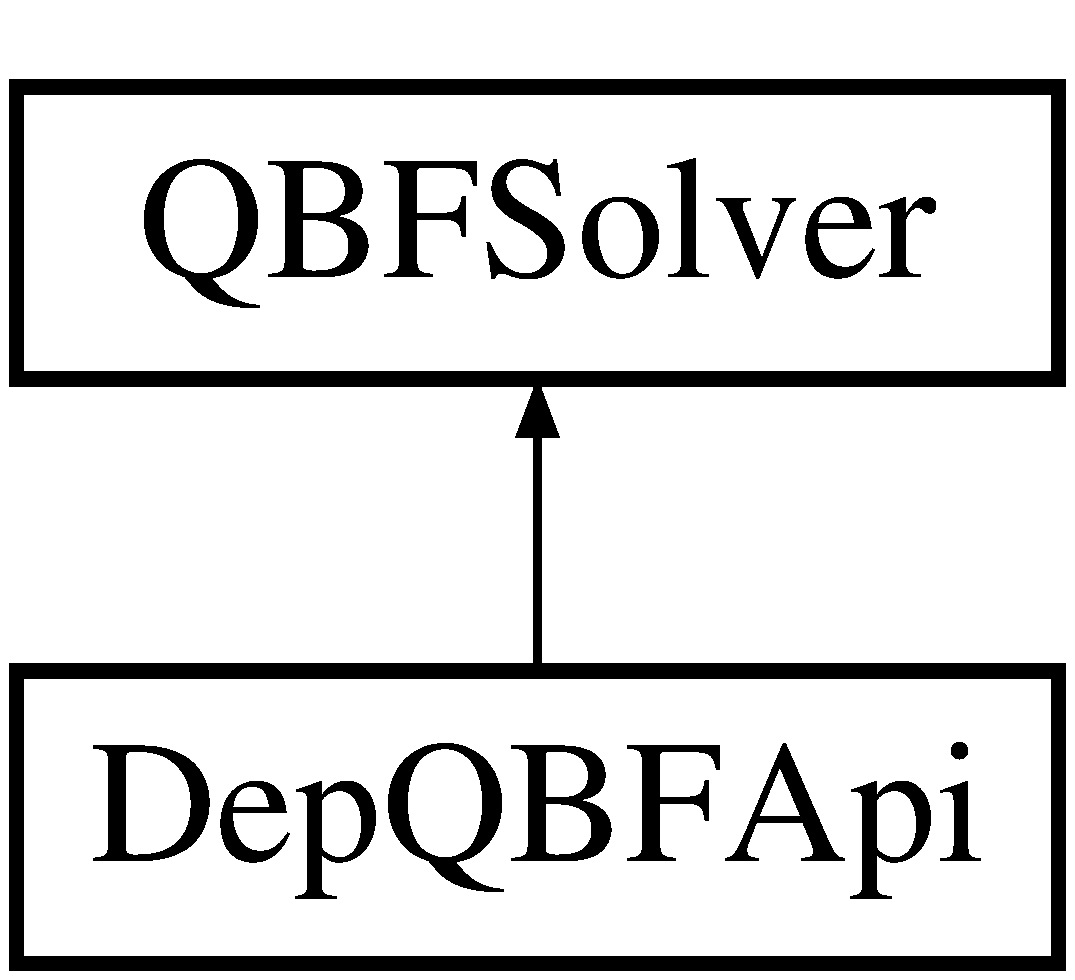
\includegraphics[height=2.000000cm]{classDepQBFApi}
\end{center}
\end{figure}
\subsection*{Public Types}
\begin{DoxyCompactItemize}
\item 
enum \hyperlink{classQBFSolver_ac091e263cb55286cc07b2451bcf4d3c7}{Quant} \{ \hyperlink{classQBFSolver_ac091e263cb55286cc07b2451bcf4d3c7a090ab4a5b262710ccd80e97d72f9a7b3}{E}, 
\hyperlink{classQBFSolver_ac091e263cb55286cc07b2451bcf4d3c7afd6518d5d985aa8346ac071e4c0d8ee0}{A}
 \}
\begin{DoxyCompactList}\small\item\em A type for the different kinds of quantifiers. \end{DoxyCompactList}\end{DoxyCompactItemize}
\subsection*{Public Member Functions}
\begin{DoxyCompactItemize}
\item 
\hyperlink{classDepQBFApi_a07fe68fc15e26247526ed06377c0a207}{Dep\-Q\-B\-F\-Api} (bool use\-\_\-bloqqer=false)
\begin{DoxyCompactList}\small\item\em Constructor. \end{DoxyCompactList}\item 
virtual \hyperlink{classDepQBFApi_ab9ce72ab0d48d1e1b6c6ffaf31ec46d6}{$\sim$\-Dep\-Q\-B\-F\-Api} ()
\begin{DoxyCompactList}\small\item\em Destructor. \end{DoxyCompactList}\item 
virtual bool \hyperlink{classDepQBFApi_a1f755841365d67f4c704bf919cb4f8b5}{is\-Sat} (const vector$<$ pair$<$ \hyperlink{classVarInfo_a64d1da76cf84fe674e5fef9764ef11cf}{Var\-Info\-::\-Var\-Kind}, \hyperlink{classQBFSolver_ac091e263cb55286cc07b2451bcf4d3c7}{Quant} $>$ $>$ \&quantifier\-\_\-prefix, const \hyperlink{classCNF}{C\-N\-F} \&cnf)
\begin{DoxyCompactList}\small\item\em Checks if a given Q\-B\-F is satisfiable (with quantification over variable kinds). \end{DoxyCompactList}\item 
virtual bool \hyperlink{classDepQBFApi_a8b220fef622b400b37d8298f29826938}{is\-Sat} (const vector$<$ pair$<$ vector$<$ int $>$, \hyperlink{classQBFSolver_ac091e263cb55286cc07b2451bcf4d3c7}{Quant} $>$ $>$ \&quantifier\-\_\-prefix, const \hyperlink{classCNF}{C\-N\-F} \&cnf)
\begin{DoxyCompactList}\small\item\em Checks if a given Q\-B\-F is satisfiable (with quantification over variable sets). \end{DoxyCompactList}\item 
virtual bool \hyperlink{classDepQBFApi_af70faa0b2136fe04e2a22743f2ca7c8e}{is\-Sat\-Model} (const vector$<$ pair$<$ \hyperlink{classVarInfo_a64d1da76cf84fe674e5fef9764ef11cf}{Var\-Info\-::\-Var\-Kind}, \hyperlink{classQBFSolver_ac091e263cb55286cc07b2451bcf4d3c7}{Quant} $>$ $>$ \&quantifier\-\_\-prefix, const \hyperlink{classCNF}{C\-N\-F} \&cnf, vector$<$ int $>$ \&model)
\begin{DoxyCompactList}\small\item\em Checks satisfiability and extracts a model (quantifying over variable kinds). \end{DoxyCompactList}\item 
virtual bool \hyperlink{classDepQBFApi_a4278bfb0cf01f21e9aa6333e14e4f5af}{is\-Sat\-Model} (const vector$<$ pair$<$ vector$<$ int $>$, \hyperlink{classQBFSolver_ac091e263cb55286cc07b2451bcf4d3c7}{Quant} $>$ $>$ \&quantifier\-\_\-prefix, const \hyperlink{classCNF}{C\-N\-F} \&cnf, vector$<$ int $>$ \&model)
\begin{DoxyCompactList}\small\item\em Checks satisfiability and extracts a model (quantifying over variable sets). \end{DoxyCompactList}\item 
virtual void \hyperlink{classDepQBFApi_a35fa14f374a196a2270baa1945e33050}{start\-Incremental\-Session} (const vector$<$ pair$<$ \hyperlink{classVarInfo_a64d1da76cf84fe674e5fef9764ef11cf}{Var\-Info\-::\-Var\-Kind}, \hyperlink{classQBFSolver_ac091e263cb55286cc07b2451bcf4d3c7}{Quant} $>$ $>$ \&quantifier\-\_\-prefix)
\begin{DoxyCompactList}\small\item\em Starts an incremental session with a quantifier prefix over variable kinds. \end{DoxyCompactList}\item 
virtual void \hyperlink{classDepQBFApi_add8abd2d970c037034012ebc21982c7e}{start\-Incremental\-Session} (const vector$<$ pair$<$ vector$<$ int $>$, \hyperlink{classQBFSolver_ac091e263cb55286cc07b2451bcf4d3c7}{Quant} $>$ $>$ \&quantifier\-\_\-prefix)
\begin{DoxyCompactList}\small\item\em Starts an incremental session with a quantifier prefix over variable sets. \end{DoxyCompactList}\item 
void \hyperlink{classDepQBFApi_a27bd21f37d83710250f9efeaeb9ad339}{do\-Min\-Cores} (bool min\-\_\-cores=true)
\begin{DoxyCompactList}\small\item\em Enables or disables the computation of M\-I\-N\-I\-M\-A\-L unsatisfiable cores. \end{DoxyCompactList}\item 
virtual void \hyperlink{classDepQBFApi_a4cacfbb0e933d8a66bd24ce5b71ea623}{clear\-Incremental\-Session} ()
\begin{DoxyCompactList}\small\item\em Closes a previously opened incremental session and frees all resources. \end{DoxyCompactList}\item 
virtual void \hyperlink{classDepQBFApi_ade58f545f2718850946391be977a6f9c}{inc\-Add\-Var\-At\-Innermost\-Quant} (int var)
\begin{DoxyCompactList}\small\item\em Declares a new variable in the innermost quantifier nesting. \end{DoxyCompactList}\item 
virtual void \hyperlink{classDepQBFApi_a1b3d100b4d70dd1200c8feb2d39accc6}{inc\-Add\-C\-N\-F} (const \hyperlink{classCNF}{C\-N\-F} \&cnf)
\begin{DoxyCompactList}\small\item\em Adds (conjuncts) a new \hyperlink{classCNF}{C\-N\-F} to the current incremental session. \end{DoxyCompactList}\item 
virtual void \hyperlink{classDepQBFApi_a76e51267fbf2c2a127ad874187bcf29a}{inc\-Add\-Clause} (const vector$<$ int $>$ \&clause)
\begin{DoxyCompactList}\small\item\em Adds (conjuncts) a new clause to the current incremental session. \end{DoxyCompactList}\item 
virtual void \hyperlink{classDepQBFApi_aa5755c46502a6016c48d6764ff087781}{inc\-Add\-Unit\-Clause} (int lit)
\begin{DoxyCompactList}\small\item\em Adds a new unit clause to the current incremental session. \end{DoxyCompactList}\item 
virtual void \hyperlink{classDepQBFApi_ab8e5a5e0adb6644ae6100afb07800dc3}{inc\-Add2\-Lit\-Clause} (int lit1, int lit2)
\begin{DoxyCompactList}\small\item\em Adds a new clause consisting of 2 literals to the current incremental session. \end{DoxyCompactList}\item 
virtual void \hyperlink{classDepQBFApi_a7300b61f89a10da1e6a679a3fd6ba9bc}{inc\-Add3\-Lit\-Clause} (int lit1, int lit2, int lit3)
\begin{DoxyCompactList}\small\item\em Adds a new clause consisting of 3 literals to the current incremental session. \end{DoxyCompactList}\item 
virtual void \hyperlink{classDepQBFApi_a97e3e631830a5fcdf351ae4bfbb336c5}{inc\-Add\-Cube} (const vector$<$ int $>$ \&cube)
\begin{DoxyCompactList}\small\item\em Adds (conjuncts) a new cube to the current incremental session. \end{DoxyCompactList}\item 
virtual void \hyperlink{classDepQBFApi_ad519a83a3e70e0224329f9e4a534a01f}{inc\-Add\-Neg\-Cube\-As\-Clause} (const vector$<$ int $>$ \&cube)
\begin{DoxyCompactList}\small\item\em Adds the negation of a given cube (which is a clause) to the incremental session. \end{DoxyCompactList}\item 
virtual void \hyperlink{classDepQBFApi_abb9f9d11ceb7f5528efd374a4fb3a7e9}{inc\-Push} ()
\begin{DoxyCompactList}\small\item\em Stores the current state of the incremental session on a stack. \end{DoxyCompactList}\item 
virtual void \hyperlink{classDepQBFApi_ac70d54cdcd3be4bc80dc84dd14e4a8c1}{inc\-Pop} ()
\begin{DoxyCompactList}\small\item\em Restores the incremental session back to the point where \hyperlink{classDepQBFApi_abb9f9d11ceb7f5528efd374a4fb3a7e9}{inc\-Push()} was called. \end{DoxyCompactList}\item 
virtual bool \hyperlink{classDepQBFApi_a8687c635b0d7f6413baca131ae9628ca}{inc\-Is\-Sat} ()
\begin{DoxyCompactList}\small\item\em Checks if the Q\-B\-F in the current incremental session is satisfiable. \end{DoxyCompactList}\item 
virtual bool \hyperlink{classDepQBFApi_a9dc678ea88f60ea0d69bddeb47f56f80}{inc\-Is\-Sat} (const vector$<$ int $>$ \&assumptions)
\begin{DoxyCompactList}\small\item\em Checks if the Q\-B\-F in the incremental session is satisfiable under assumptions. \end{DoxyCompactList}\item 
virtual bool \hyperlink{classDepQBFApi_ab2129624aca73b877c16a5fc7b17f95f}{inc\-Is\-Sat\-Model\-Or\-Core} (const vector$<$ int $>$ \&assumptions, vector$<$ int $>$ \&model\-\_\-or\-\_\-core)
\begin{DoxyCompactList}\small\item\em Checks if the incremental session is satisfiable and computes a model or core. \end{DoxyCompactList}\item 
virtual bool \hyperlink{classDepQBFApi_a218feb52145bd715dc07fa2b765662f4}{inc\-Is\-Sat\-Model} (const vector$<$ int $>$ \&assumptions, vector$<$ int $>$ \&model)
\begin{DoxyCompactList}\small\item\em Checks if the incremental session is satisfiable and computes a model. \end{DoxyCompactList}\item 
virtual bool \hyperlink{classDepQBFApi_a4290fa5559f2ba9663bdb158c384cc92}{inc\-Is\-Sat\-Core} (const vector$<$ int $>$ \&assumptions, vector$<$ int $>$ \&core)
\begin{DoxyCompactList}\small\item\em Checks if the incremental session is satisfiable and computes a core. \end{DoxyCompactList}\item 
void \hyperlink{classDepQBFApi_ae90857fc6480bec580154f878731f740}{debug\-Dump\-Inc\-Solver\-State} ()
\begin{DoxyCompactList}\small\item\em Dumps the incremental solver state for debugging purposes. \end{DoxyCompactList}\end{DoxyCompactItemize}
\subsection*{Protected Member Functions}
\begin{DoxyCompactItemize}
\item 
void \hyperlink{classDepQBFApi_ac6a024dbf9355b9d7b17f8181642e469}{init\-Bloqqer} (const vector$<$ pair$<$ \hyperlink{classVarInfo_a64d1da76cf84fe674e5fef9764ef11cf}{Var\-Info\-::\-Var\-Kind}, \hyperlink{classQBFSolver_ac091e263cb55286cc07b2451bcf4d3c7}{Quant} $>$ $>$ \&quantifier\-\_\-prefix, const \hyperlink{classCNF}{C\-N\-F} \&cnf)
\begin{DoxyCompactList}\small\item\em Initializes the pre-\/processor with a Q\-B\-F (quantifying over variable kinds). \end{DoxyCompactList}\item 
void \hyperlink{classDepQBFApi_a5f7ea6239edb4d78bbda33091f51cdf5}{init\-Bloqqer} (const vector$<$ pair$<$ vector$<$ int $>$, \hyperlink{classQBFSolver_ac091e263cb55286cc07b2451bcf4d3c7}{Quant} $>$ $>$ \&quantifier\-\_\-prefix, const \hyperlink{classCNF}{C\-N\-F} \&cnf)
\begin{DoxyCompactList}\small\item\em Initializes the pre-\/processor with a Q\-B\-F (quantifying over variable sets). \end{DoxyCompactList}\item 
void \hyperlink{classDepQBFApi_a2f99baf1fb6759458979e799ce706bc4}{init\-Dep\-Q\-B\-F} (Q\-D\-P\-L\-L $\ast$solver, const vector$<$ pair$<$ \hyperlink{classVarInfo_a64d1da76cf84fe674e5fef9764ef11cf}{Var\-Info\-::\-Var\-Kind}, \hyperlink{classQBFSolver_ac091e263cb55286cc07b2451bcf4d3c7}{Quant} $>$ $>$ \&quantifier\-\_\-prefix, const \hyperlink{classCNF}{C\-N\-F} \&cnf)
\begin{DoxyCompactList}\small\item\em Initializes a Dep\-Q\-B\-F instance with a Q\-B\-F (quantifying over variable kinds). \end{DoxyCompactList}\item 
void \hyperlink{classDepQBFApi_af1e78176cae55e6a76e193d216b5a3dc}{init\-Dep\-Q\-B\-F} (Q\-D\-P\-L\-L $\ast$solver, const vector$<$ pair$<$ vector$<$ int $>$, \hyperlink{classQBFSolver_ac091e263cb55286cc07b2451bcf4d3c7}{Quant} $>$ $>$ \&quantifier\-\_\-prefix, const \hyperlink{classCNF}{C\-N\-F} \&cnf)
\begin{DoxyCompactList}\small\item\em Initializes a Dep\-Q\-B\-F instance with a Q\-B\-F (quantifying over variable sets). \end{DoxyCompactList}\item 
void \hyperlink{classDepQBFApi_ad65a2e0366a4af8e3a436cf3b8ef5721}{extract\-Core} (Q\-D\-P\-L\-L $\ast$solver, vector$<$ int $>$ \&core)
\begin{DoxyCompactList}\small\item\em Extracts an unsatisfiable core after unsatisfiability has been shown. \end{DoxyCompactList}\item 
void \hyperlink{classDepQBFApi_a3a24cd04a3ddc626f2933429dda4e3b9}{debug\-Check\-Bloqqer\-Verdict} (int bloqqer\-\_\-verdict, const vector$<$ pair$<$ \hyperlink{classVarInfo_a64d1da76cf84fe674e5fef9764ef11cf}{Var\-Info\-::\-Var\-Kind}, \hyperlink{classQBFSolver_ac091e263cb55286cc07b2451bcf4d3c7}{Quant} $>$ $>$ \&quantifier\-\_\-prefix, const \hyperlink{classCNF}{C\-N\-F} \&cnf)
\begin{DoxyCompactList}\small\item\em A debug function to cross-\/check bloqqer verdicts (S\-A\-T or U\-N\-S\-A\-T). \end{DoxyCompactList}\item 
void \hyperlink{classDepQBFApi_afe717cb04d4bd6223bca3e52ba2c7e1f}{debug\-Check\-Bloqqer\-Verdict} (int bloqqer\-\_\-verdict, const vector$<$ pair$<$ vector$<$ int $>$, \hyperlink{classQBFSolver_ac091e263cb55286cc07b2451bcf4d3c7}{Quant} $>$ $>$ \&quantifier\-\_\-prefix, const \hyperlink{classCNF}{C\-N\-F} \&cnf)
\begin{DoxyCompactList}\small\item\em A debug function to cross-\/check bloqqer verdicts (S\-A\-T or U\-N\-S\-A\-T). \end{DoxyCompactList}\item 
void \hyperlink{classDepQBFApi_a55a75bae106e42f6df73fb129a18b4bb}{debug\-Check\-Bloqqer\-Model} (const vector$<$ int $>$ \&model, const vector$<$ pair$<$ \hyperlink{classVarInfo_a64d1da76cf84fe674e5fef9764ef11cf}{Var\-Info\-::\-Var\-Kind}, \hyperlink{classQBFSolver_ac091e263cb55286cc07b2451bcf4d3c7}{Quant} $>$ $>$ \&quantifier\-\_\-prefix, const \hyperlink{classCNF}{C\-N\-F} \&cnf)
\begin{DoxyCompactList}\small\item\em A debug function to cross-\/check models produced by bloqqer. \end{DoxyCompactList}\item 
void \hyperlink{classDepQBFApi_ab8f1fa3fa93a7c6877b22579305f22f5}{debug\-Check\-Bloqqer\-Model} (const vector$<$ int $>$ \&model, const vector$<$ pair$<$ vector$<$ int $>$, \hyperlink{classQBFSolver_ac091e263cb55286cc07b2451bcf4d3c7}{Quant} $>$ $>$ \&quantifier\-\_\-prefix, const \hyperlink{classCNF}{C\-N\-F} \&cnf)
\begin{DoxyCompactList}\small\item\em A debug function to cross-\/check models produced by bloqqer. \end{DoxyCompactList}\item 
void \hyperlink{classDepQBFApi_a6731d3b5e3c5d89f2b3d9e2056ca93f6}{debug\-Assert\-Is\-Declared\-Inc} (int lit) const 
\begin{DoxyCompactList}\small\item\em Asserts that a literal has been declared in the current incremental session. \end{DoxyCompactList}\end{DoxyCompactItemize}
\subsection*{Protected Attributes}
\begin{DoxyCompactItemize}
\item 
bool \hyperlink{classDepQBFApi_a04798225c77a19a1d2f415e50b93cfb1}{use\-\_\-bloqqer\-\_\-}
\begin{DoxyCompactList}\small\item\em A flag indicating whether or not the pre-\/processor bloqqer should be used. \end{DoxyCompactList}\item 
bool \hyperlink{classDepQBFApi_aeba411424d6185767325936d2ccf11de}{min\-\_\-cores\-\_\-}
\begin{DoxyCompactList}\small\item\em A flag indicating whether or not unsatisfiable cores should be further minimized. \end{DoxyCompactList}\item 
Q\-D\-P\-L\-L $\ast$ \hyperlink{classDepQBFApi_a22f9645648890b1997e702743fc2e8fe}{inc\-\_\-solver\-\_\-}
\begin{DoxyCompactList}\small\item\em The solver instance to use in the incremental session. \end{DoxyCompactList}\item 
vector$<$ int $>$ \hyperlink{classDepQBFApi_a45305a0f7bb106f43eb7d12554e71564}{inc\-\_\-model\-\_\-vars\-\_\-}
\begin{DoxyCompactList}\small\item\em The variables for which a satisfying assignment can be constructed. \end{DoxyCompactList}\item 
set$<$ int $>$ \hyperlink{classDepQBFApi_a28c913cc99ac6671a2f86dafe1c9f55a}{inc\-\_\-decl\-\_\-vars\-\_\-}
\begin{DoxyCompactList}\small\item\em The variables which have been declared in the current incremental session. \end{DoxyCompactList}\end{DoxyCompactItemize}
\subsection*{Private Member Functions}
\begin{DoxyCompactItemize}
\item 
\hyperlink{classDepQBFApi_ab7f7fe54d8ebfd6dc49296e10efada92}{Dep\-Q\-B\-F\-Api} (const \hyperlink{classDepQBFApi}{Dep\-Q\-B\-F\-Api} \&other)
\begin{DoxyCompactList}\small\item\em Copy constructor. \end{DoxyCompactList}\item 
\hyperlink{classDepQBFApi}{Dep\-Q\-B\-F\-Api} \& \hyperlink{classDepQBFApi_ac92d8d42313774de6ce7f3bb2ca121c0}{operator=} (const \hyperlink{classDepQBFApi}{Dep\-Q\-B\-F\-Api} \&other)
\begin{DoxyCompactList}\small\item\em Assignment operator. \end{DoxyCompactList}\end{DoxyCompactItemize}


\subsection{Detailed Description}
Interfaces the Dep\-Q\-B\-F Q\-B\-F-\/solver via its A\-P\-I. 

This class represents an interface to the Q\-B\-F-\/solver Dep\-Q\-B\-F (see \href{https://github.com/lonsing/depqbf}{\tt https\-://github.\-com/lonsing/depqbf}). For a given Quantified Boolean formula (a \hyperlink{classCNF}{C\-N\-F} with a quantifier prefix), this class is able to determine satisfiability. Furthermore, in case of satisfiability, it can extract satisfying assignments for variables quantified existentially on the outermost level.

This interface to Dep\-Q\-B\-F can operated in two modes\-: with and without Bloqqer as pre-\/processor.

\begin{DoxyAuthor}{Author}
Robert Koenighofer (\href{mailto:robert.koenighofer@iaik.tugraz.at}{\tt robert.\-koenighofer@iaik.\-tugraz.\-at}) 
\end{DoxyAuthor}
\begin{DoxyVersion}{Version}
1.\-2.\-0 
\end{DoxyVersion}


Definition at line 54 of file Dep\-Q\-B\-F\-Api.\-h.



\subsection{Member Enumeration Documentation}
\hypertarget{classQBFSolver_ac091e263cb55286cc07b2451bcf4d3c7}{\index{Dep\-Q\-B\-F\-Api@{Dep\-Q\-B\-F\-Api}!Quant@{Quant}}
\index{Quant@{Quant}!DepQBFApi@{Dep\-Q\-B\-F\-Api}}
\subsubsection[{Quant}]{\setlength{\rightskip}{0pt plus 5cm}enum {\bf Q\-B\-F\-Solver\-::\-Quant}\hspace{0.3cm}{\ttfamily [inherited]}}}\label{classQBFSolver_ac091e263cb55286cc07b2451bcf4d3c7}


A type for the different kinds of quantifiers. 

\begin{Desc}
\item[Enumerator]\par
\begin{description}
\index{E@{E}!Dep\-Q\-B\-F\-Api@{Dep\-Q\-B\-F\-Api}}\index{Dep\-Q\-B\-F\-Api@{Dep\-Q\-B\-F\-Api}!E@{E}}\item[{\em 
\hypertarget{classQBFSolver_ac091e263cb55286cc07b2451bcf4d3c7a090ab4a5b262710ccd80e97d72f9a7b3}{E}\label{classQBFSolver_ac091e263cb55286cc07b2451bcf4d3c7a090ab4a5b262710ccd80e97d72f9a7b3}
}]The value for existential quantification. \index{A@{A}!Dep\-Q\-B\-F\-Api@{Dep\-Q\-B\-F\-Api}}\index{Dep\-Q\-B\-F\-Api@{Dep\-Q\-B\-F\-Api}!A@{A}}\item[{\em 
\hypertarget{classQBFSolver_ac091e263cb55286cc07b2451bcf4d3c7afd6518d5d985aa8346ac071e4c0d8ee0}{A}\label{classQBFSolver_ac091e263cb55286cc07b2451bcf4d3c7afd6518d5d985aa8346ac071e4c0d8ee0}
}]The value for universal quantification. \end{description}
\end{Desc}


Definition at line 56 of file Q\-B\-F\-Solver.\-h.



\subsection{Constructor \& Destructor Documentation}
\hypertarget{classDepQBFApi_a07fe68fc15e26247526ed06377c0a207}{\index{Dep\-Q\-B\-F\-Api@{Dep\-Q\-B\-F\-Api}!Dep\-Q\-B\-F\-Api@{Dep\-Q\-B\-F\-Api}}
\index{Dep\-Q\-B\-F\-Api@{Dep\-Q\-B\-F\-Api}!DepQBFApi@{Dep\-Q\-B\-F\-Api}}
\subsubsection[{Dep\-Q\-B\-F\-Api}]{\setlength{\rightskip}{0pt plus 5cm}Dep\-Q\-B\-F\-Api\-::\-Dep\-Q\-B\-F\-Api (
\begin{DoxyParamCaption}
\item[{bool}]{use\-\_\-bloqqer = {\ttfamily false}}
\end{DoxyParamCaption}
)}}\label{classDepQBFApi_a07fe68fc15e26247526ed06377c0a207}


Constructor. 


\begin{DoxyParams}{Parameters}
{\em use\-\_\-bloqqer} & True if bloqqer should be used as pre-\/processor, false if no pre-\/processing should be used. If this parameter is omitted, no pre-\/processing is used. At the moment, incremental solving is always done without any pre-\/processing. \\
\hline
\end{DoxyParams}


Definition at line 44 of file Dep\-Q\-B\-F\-Api.\-cpp.

\hypertarget{classDepQBFApi_ab9ce72ab0d48d1e1b6c6ffaf31ec46d6}{\index{Dep\-Q\-B\-F\-Api@{Dep\-Q\-B\-F\-Api}!$\sim$\-Dep\-Q\-B\-F\-Api@{$\sim$\-Dep\-Q\-B\-F\-Api}}
\index{$\sim$\-Dep\-Q\-B\-F\-Api@{$\sim$\-Dep\-Q\-B\-F\-Api}!DepQBFApi@{Dep\-Q\-B\-F\-Api}}
\subsubsection[{$\sim$\-Dep\-Q\-B\-F\-Api}]{\setlength{\rightskip}{0pt plus 5cm}Dep\-Q\-B\-F\-Api\-::$\sim$\-Dep\-Q\-B\-F\-Api (
\begin{DoxyParamCaption}
{}
\end{DoxyParamCaption}
)\hspace{0.3cm}{\ttfamily [virtual]}}}\label{classDepQBFApi_ab9ce72ab0d48d1e1b6c6ffaf31ec46d6}


Destructor. 



Definition at line 53 of file Dep\-Q\-B\-F\-Api.\-cpp.



References clear\-Incremental\-Session().

\hypertarget{classDepQBFApi_ab7f7fe54d8ebfd6dc49296e10efada92}{\index{Dep\-Q\-B\-F\-Api@{Dep\-Q\-B\-F\-Api}!Dep\-Q\-B\-F\-Api@{Dep\-Q\-B\-F\-Api}}
\index{Dep\-Q\-B\-F\-Api@{Dep\-Q\-B\-F\-Api}!DepQBFApi@{Dep\-Q\-B\-F\-Api}}
\subsubsection[{Dep\-Q\-B\-F\-Api}]{\setlength{\rightskip}{0pt plus 5cm}Dep\-Q\-B\-F\-Api\-::\-Dep\-Q\-B\-F\-Api (
\begin{DoxyParamCaption}
\item[{const {\bf Dep\-Q\-B\-F\-Api} \&}]{other}
\end{DoxyParamCaption}
)\hspace{0.3cm}{\ttfamily [private]}}}\label{classDepQBFApi_ab7f7fe54d8ebfd6dc49296e10efada92}


Copy constructor. 

The copy constructor is disabled (set private) and not implemented.


\begin{DoxyParams}{Parameters}
{\em other} & The source for creating the copy. \\
\hline
\end{DoxyParams}


\subsection{Member Function Documentation}
\hypertarget{classDepQBFApi_a4cacfbb0e933d8a66bd24ce5b71ea623}{\index{Dep\-Q\-B\-F\-Api@{Dep\-Q\-B\-F\-Api}!clear\-Incremental\-Session@{clear\-Incremental\-Session}}
\index{clear\-Incremental\-Session@{clear\-Incremental\-Session}!DepQBFApi@{Dep\-Q\-B\-F\-Api}}
\subsubsection[{clear\-Incremental\-Session}]{\setlength{\rightskip}{0pt plus 5cm}void Dep\-Q\-B\-F\-Api\-::clear\-Incremental\-Session (
\begin{DoxyParamCaption}
{}
\end{DoxyParamCaption}
)\hspace{0.3cm}{\ttfamily [virtual]}}}\label{classDepQBFApi_a4cacfbb0e933d8a66bd24ce5b71ea623}


Closes a previously opened incremental session and frees all resources. 

If no incremental session is open, then this method has no effect at all. 

Definition at line 404 of file Dep\-Q\-B\-F\-Api.\-cpp.



References inc\-\_\-decl\-\_\-vars\-\_\-, inc\-\_\-model\-\_\-vars\-\_\-, and inc\-\_\-solver\-\_\-.



Referenced by $\sim$\-Dep\-Q\-B\-F\-Api().

\hypertarget{classDepQBFApi_a6731d3b5e3c5d89f2b3d9e2056ca93f6}{\index{Dep\-Q\-B\-F\-Api@{Dep\-Q\-B\-F\-Api}!debug\-Assert\-Is\-Declared\-Inc@{debug\-Assert\-Is\-Declared\-Inc}}
\index{debug\-Assert\-Is\-Declared\-Inc@{debug\-Assert\-Is\-Declared\-Inc}!DepQBFApi@{Dep\-Q\-B\-F\-Api}}
\subsubsection[{debug\-Assert\-Is\-Declared\-Inc}]{\setlength{\rightskip}{0pt plus 5cm}void Dep\-Q\-B\-F\-Api\-::debug\-Assert\-Is\-Declared\-Inc (
\begin{DoxyParamCaption}
\item[{int}]{lit}
\end{DoxyParamCaption}
) const\hspace{0.3cm}{\ttfamily [protected]}}}\label{classDepQBFApi_a6731d3b5e3c5d89f2b3d9e2056ca93f6}


Asserts that a literal has been declared in the current incremental session. 

Asserts that a certain literal has been declared in the quantifier prefix of the current incremental session. This check is done in the debug mode only.


\begin{DoxyParams}{Parameters}
{\em lit} & The literal to check. \\
\hline
\end{DoxyParams}


Definition at line 1028 of file Dep\-Q\-B\-F\-Api.\-cpp.



References D\-A\-S\-S\-E\-R\-T, and inc\-\_\-decl\-\_\-vars\-\_\-.



Referenced by inc\-Add2\-Lit\-Clause(), inc\-Add3\-Lit\-Clause(), inc\-Add\-Clause(), inc\-Add\-C\-N\-F(), inc\-Add\-Cube(), inc\-Add\-Neg\-Cube\-As\-Clause(), inc\-Add\-Unit\-Clause(), inc\-Is\-Sat(), inc\-Is\-Sat\-Core(), inc\-Is\-Sat\-Model(), and inc\-Is\-Sat\-Model\-Or\-Core().

\hypertarget{classDepQBFApi_a55a75bae106e42f6df73fb129a18b4bb}{\index{Dep\-Q\-B\-F\-Api@{Dep\-Q\-B\-F\-Api}!debug\-Check\-Bloqqer\-Model@{debug\-Check\-Bloqqer\-Model}}
\index{debug\-Check\-Bloqqer\-Model@{debug\-Check\-Bloqqer\-Model}!DepQBFApi@{Dep\-Q\-B\-F\-Api}}
\subsubsection[{debug\-Check\-Bloqqer\-Model}]{\setlength{\rightskip}{0pt plus 5cm}void Dep\-Q\-B\-F\-Api\-::debug\-Check\-Bloqqer\-Model (
\begin{DoxyParamCaption}
\item[{const vector$<$ int $>$ \&}]{model, }
\item[{const vector$<$ pair$<$ {\bf Var\-Info\-::\-Var\-Kind}, {\bf Quant} $>$ $>$ \&}]{quantifier\-\_\-prefix, }
\item[{const {\bf C\-N\-F} \&}]{cnf}
\end{DoxyParamCaption}
)\hspace{0.3cm}{\ttfamily [protected]}}}\label{classDepQBFApi_a55a75bae106e42f6df73fb129a18b4bb}


A debug function to cross-\/check models produced by bloqqer. 

Dep\-Q\-B\-F without preprocessing is used to check if the model found by bloqqer indeed satisfies the Q\-B\-F. This method is used to debug bloqqer.


\begin{DoxyParams}{Parameters}
{\em model} & The satisfying assignment found by bloqqer. Negated variables in the vector are F\-A\-L\-S\-E, unnegated ones are T\-R\-U\-E. \\
\hline
{\em quantifier\-\_\-prefix} & The quantifier prefix as a vector of pairs. vector\mbox{[}0\mbox{]} is the leftmost (i.\-e., outermost) quantifier block. The pairs in the quantifier\-\_\-prefix assign an existential or universal quantifier to every kind of variable that occurs in the cnf. \\
\hline
{\em cnf} & A Boolean formula in \hyperlink{classCNF}{C\-N\-F}. \\
\hline
\end{DoxyParams}


Definition at line 935 of file Dep\-Q\-B\-F\-Api.\-cpp.



References C\-N\-F\-::add\-Cube(), Utils\-::debug\-Print(), Ext\-Q\-B\-F\-Solver\-::dump\-Q\-B\-F(), Var\-Manager\-::get\-Vars\-Of\-Type(), Var\-Manager\-::instance(), is\-Sat(), L\-\_\-\-E\-R\-R, and M\-A\-S\-S\-E\-R\-T.

\hypertarget{classDepQBFApi_ab8f1fa3fa93a7c6877b22579305f22f5}{\index{Dep\-Q\-B\-F\-Api@{Dep\-Q\-B\-F\-Api}!debug\-Check\-Bloqqer\-Model@{debug\-Check\-Bloqqer\-Model}}
\index{debug\-Check\-Bloqqer\-Model@{debug\-Check\-Bloqqer\-Model}!DepQBFApi@{Dep\-Q\-B\-F\-Api}}
\subsubsection[{debug\-Check\-Bloqqer\-Model}]{\setlength{\rightskip}{0pt plus 5cm}void Dep\-Q\-B\-F\-Api\-::debug\-Check\-Bloqqer\-Model (
\begin{DoxyParamCaption}
\item[{const vector$<$ int $>$ \&}]{model, }
\item[{const vector$<$ pair$<$ vector$<$ int $>$, {\bf Quant} $>$ $>$ \&}]{quantifier\-\_\-prefix, }
\item[{const {\bf C\-N\-F} \&}]{cnf}
\end{DoxyParamCaption}
)\hspace{0.3cm}{\ttfamily [protected]}}}\label{classDepQBFApi_ab8f1fa3fa93a7c6877b22579305f22f5}


A debug function to cross-\/check models produced by bloqqer. 

Dep\-Q\-B\-F without preprocessing is used to check if the model found by bloqqer indeed satisfies the Q\-B\-F. This method is used to debug bloqqer.


\begin{DoxyParams}{Parameters}
{\em model} & The satisfying assignment found by bloqqer. Negated variables in the vector are F\-A\-L\-S\-E, unnegated ones are T\-R\-U\-E. \\
\hline
{\em quantifier\-\_\-prefix} & The quantifier prefix as a vector of pairs. vector\mbox{[}0\mbox{]} is the leftmost (i.\-e., outermost) quantifier block. The pairs in the quantifier\-\_\-prefix assign an existential or universal quantifier to different sets of variables occurring in the cnf. \\
\hline
{\em cnf} & A Boolean formula in \hyperlink{classCNF}{C\-N\-F}. \\
\hline
\end{DoxyParams}


Definition at line 982 of file Dep\-Q\-B\-F\-Api.\-cpp.



References C\-N\-F\-::add\-Cube(), Utils\-::debug\-Print(), Ext\-Q\-B\-F\-Solver\-::dump\-Q\-B\-F(), is\-Sat(), L\-\_\-\-E\-R\-R, and M\-A\-S\-S\-E\-R\-T.

\hypertarget{classDepQBFApi_a3a24cd04a3ddc626f2933429dda4e3b9}{\index{Dep\-Q\-B\-F\-Api@{Dep\-Q\-B\-F\-Api}!debug\-Check\-Bloqqer\-Verdict@{debug\-Check\-Bloqqer\-Verdict}}
\index{debug\-Check\-Bloqqer\-Verdict@{debug\-Check\-Bloqqer\-Verdict}!DepQBFApi@{Dep\-Q\-B\-F\-Api}}
\subsubsection[{debug\-Check\-Bloqqer\-Verdict}]{\setlength{\rightskip}{0pt plus 5cm}void Dep\-Q\-B\-F\-Api\-::debug\-Check\-Bloqqer\-Verdict (
\begin{DoxyParamCaption}
\item[{int}]{bloqqer\-\_\-verdict, }
\item[{const vector$<$ pair$<$ {\bf Var\-Info\-::\-Var\-Kind}, {\bf Quant} $>$ $>$ \&}]{quantifier\-\_\-prefix, }
\item[{const {\bf C\-N\-F} \&}]{cnf}
\end{DoxyParamCaption}
)\hspace{0.3cm}{\ttfamily [protected]}}}\label{classDepQBFApi_a3a24cd04a3ddc626f2933429dda4e3b9}


A debug function to cross-\/check bloqqer verdicts (S\-A\-T or U\-N\-S\-A\-T). 

The Q\-B\-F is also solved with Dep\-Q\-B\-F without pre-\/processing and the two verdicts are compared. This method is used to debug bloqqer.


\begin{DoxyParams}{Parameters}
{\em bloqqer\-\_\-verdict} & The result returned by bloqqer. The value 10 means S\-A\-T, the value 20 means U\-N\-S\-A\-T. \\
\hline
{\em quantifier\-\_\-prefix} & The quantifier prefix as a vector of pairs. vector\mbox{[}0\mbox{]} is the leftmost (i.\-e., outermost) quantifier block. The pairs in the quantifier\-\_\-prefix assign an existential or universal quantifier to every kind of variable that occurs in the cnf. \\
\hline
{\em cnf} & A Boolean formula in \hyperlink{classCNF}{C\-N\-F}. \\
\hline
\end{DoxyParams}


Definition at line 877 of file Dep\-Q\-B\-F\-Api.\-cpp.



References Ext\-Q\-B\-F\-Solver\-::dump\-Q\-B\-F(), is\-Sat(), L\-\_\-\-E\-R\-R, and M\-A\-S\-S\-E\-R\-T.



Referenced by is\-Sat\-Model().

\hypertarget{classDepQBFApi_afe717cb04d4bd6223bca3e52ba2c7e1f}{\index{Dep\-Q\-B\-F\-Api@{Dep\-Q\-B\-F\-Api}!debug\-Check\-Bloqqer\-Verdict@{debug\-Check\-Bloqqer\-Verdict}}
\index{debug\-Check\-Bloqqer\-Verdict@{debug\-Check\-Bloqqer\-Verdict}!DepQBFApi@{Dep\-Q\-B\-F\-Api}}
\subsubsection[{debug\-Check\-Bloqqer\-Verdict}]{\setlength{\rightskip}{0pt plus 5cm}void Dep\-Q\-B\-F\-Api\-::debug\-Check\-Bloqqer\-Verdict (
\begin{DoxyParamCaption}
\item[{int}]{bloqqer\-\_\-verdict, }
\item[{const vector$<$ pair$<$ vector$<$ int $>$, {\bf Quant} $>$ $>$ \&}]{quantifier\-\_\-prefix, }
\item[{const {\bf C\-N\-F} \&}]{cnf}
\end{DoxyParamCaption}
)\hspace{0.3cm}{\ttfamily [protected]}}}\label{classDepQBFApi_afe717cb04d4bd6223bca3e52ba2c7e1f}


A debug function to cross-\/check bloqqer verdicts (S\-A\-T or U\-N\-S\-A\-T). 

The Q\-B\-F is also solved with Dep\-Q\-B\-F without pre-\/processing and the two verdicts are compared. This method is used to debug bloqqer.


\begin{DoxyParams}{Parameters}
{\em bloqqer\-\_\-verdict} & The result returned by bloqqer. The value 10 means S\-A\-T, the value 20 means U\-N\-S\-A\-T. \\
\hline
{\em quantifier\-\_\-prefix} & The quantifier prefix as a vector of pairs. vector\mbox{[}0\mbox{]} is the leftmost (i.\-e., outermost) quantifier block. The pairs in the quantifier\-\_\-prefix assign an existential or universal quantifier to different sets of variables occurring in the cnf. \\
\hline
{\em cnf} & A Boolean formula in \hyperlink{classCNF}{C\-N\-F}. \\
\hline
\end{DoxyParams}


Definition at line 906 of file Dep\-Q\-B\-F\-Api.\-cpp.



References Ext\-Q\-B\-F\-Solver\-::dump\-Q\-B\-F(), is\-Sat(), L\-\_\-\-E\-R\-R, and M\-A\-S\-S\-E\-R\-T.

\hypertarget{classDepQBFApi_ae90857fc6480bec580154f878731f740}{\index{Dep\-Q\-B\-F\-Api@{Dep\-Q\-B\-F\-Api}!debug\-Dump\-Inc\-Solver\-State@{debug\-Dump\-Inc\-Solver\-State}}
\index{debug\-Dump\-Inc\-Solver\-State@{debug\-Dump\-Inc\-Solver\-State}!DepQBFApi@{Dep\-Q\-B\-F\-Api}}
\subsubsection[{debug\-Dump\-Inc\-Solver\-State}]{\setlength{\rightskip}{0pt plus 5cm}void Dep\-Q\-B\-F\-Api\-::debug\-Dump\-Inc\-Solver\-State (
\begin{DoxyParamCaption}
{}
\end{DoxyParamCaption}
)}}\label{classDepQBFApi_ae90857fc6480bec580154f878731f740}


Dumps the incremental solver state for debugging purposes. 



Definition at line 695 of file Dep\-Q\-B\-F\-Api.\-cpp.



References inc\-\_\-solver\-\_\-, and M\-A\-S\-S\-E\-R\-T.

\hypertarget{classDepQBFApi_a27bd21f37d83710250f9efeaeb9ad339}{\index{Dep\-Q\-B\-F\-Api@{Dep\-Q\-B\-F\-Api}!do\-Min\-Cores@{do\-Min\-Cores}}
\index{do\-Min\-Cores@{do\-Min\-Cores}!DepQBFApi@{Dep\-Q\-B\-F\-Api}}
\subsubsection[{do\-Min\-Cores}]{\setlength{\rightskip}{0pt plus 5cm}void Dep\-Q\-B\-F\-Api\-::do\-Min\-Cores (
\begin{DoxyParamCaption}
\item[{bool}]{min\-\_\-cores = {\ttfamily true}}
\end{DoxyParamCaption}
)}}\label{classDepQBFApi_a27bd21f37d83710250f9efeaeb9ad339}


Enables or disables the computation of M\-I\-N\-I\-M\-A\-L unsatisfiable cores. 


\begin{DoxyParams}{Parameters}
{\em min\-\_\-cores} & A flag indicating if unsatisfiable cores returned by the solver should be minimized further by trying to drop one literal after the other. This makes the calls slower but produces potentially smaller cubes. If the parameter is skipped the computation of minimal cores is enabled. \\
\hline
\end{DoxyParams}


Definition at line 398 of file Dep\-Q\-B\-F\-Api.\-cpp.



References min\-\_\-cores\-\_\-.



Referenced by Learn\-Synth\-Q\-B\-F\-Inc\-::compute\-Winning\-Region\-All(), Learn\-Synth\-Q\-B\-F\-Inc\-::compute\-Winning\-Region\-All\-Pool(), Learn\-Synth\-Q\-B\-F\-Inc\-::compute\-Winning\-Region\-All\-Push(), Learn\-Synth\-Q\-B\-F\-Inc\-::compute\-Winning\-Region\-One(), Learn\-Synth\-Q\-B\-F\-Inc\-::compute\-Winning\-Region\-One\-Pool(), Learn\-Synth\-Q\-B\-F\-Inc\-::compute\-Winning\-Region\-One\-Push(), and Clause\-Minimizer\-Q\-B\-F\-::minimize\-Clauses\-Inc().

\hypertarget{classDepQBFApi_ad65a2e0366a4af8e3a436cf3b8ef5721}{\index{Dep\-Q\-B\-F\-Api@{Dep\-Q\-B\-F\-Api}!extract\-Core@{extract\-Core}}
\index{extract\-Core@{extract\-Core}!DepQBFApi@{Dep\-Q\-B\-F\-Api}}
\subsubsection[{extract\-Core}]{\setlength{\rightskip}{0pt plus 5cm}void Dep\-Q\-B\-F\-Api\-::extract\-Core (
\begin{DoxyParamCaption}
\item[{Q\-D\-P\-L\-L $\ast$}]{solver, }
\item[{vector$<$ int $>$ \&}]{core}
\end{DoxyParamCaption}
)\hspace{0.3cm}{\ttfamily [protected]}}}\label{classDepQBFApi_ad65a2e0366a4af8e3a436cf3b8ef5721}


Extracts an unsatisfiable core after unsatisfiability has been shown. 


\begin{DoxyParams}{Parameters}
{\em solver} & The Dep\-Q\-B\-F solver instance to extract the core from. \\
\hline
{\em core} & The vector into which the resulting unsatisfiable core will be stored. It is a subset of the used assumptions. \\
\hline
\end{DoxyParams}


Definition at line 829 of file Dep\-Q\-B\-F\-Api.\-cpp.



References min\-\_\-cores\-\_\-, Utils\-::randomize(), and Utils\-::remove().



Referenced by inc\-Is\-Sat\-Core(), and inc\-Is\-Sat\-Model\-Or\-Core().

\hypertarget{classDepQBFApi_ab8e5a5e0adb6644ae6100afb07800dc3}{\index{Dep\-Q\-B\-F\-Api@{Dep\-Q\-B\-F\-Api}!inc\-Add2\-Lit\-Clause@{inc\-Add2\-Lit\-Clause}}
\index{inc\-Add2\-Lit\-Clause@{inc\-Add2\-Lit\-Clause}!DepQBFApi@{Dep\-Q\-B\-F\-Api}}
\subsubsection[{inc\-Add2\-Lit\-Clause}]{\setlength{\rightskip}{0pt plus 5cm}void Dep\-Q\-B\-F\-Api\-::inc\-Add2\-Lit\-Clause (
\begin{DoxyParamCaption}
\item[{int}]{lit1, }
\item[{int}]{lit2}
\end{DoxyParamCaption}
)\hspace{0.3cm}{\ttfamily [virtual]}}}\label{classDepQBFApi_ab8e5a5e0adb6644ae6100afb07800dc3}


Adds a new clause consisting of 2 literals to the current incremental session. 

\begin{DoxyPrecond}{Precondition}
\hyperlink{classDepQBFApi_a35fa14f374a196a2270baa1945e33050}{start\-Incremental\-Session()} must have been called before. 
\end{DoxyPrecond}

\begin{DoxyParams}{Parameters}
{\em lit1} & The first literal of the clause to add to the currently open incremental session. \\
\hline
{\em lit2} & The second literal of the clause to add to the currently open incremental session. \\
\hline
\end{DoxyParams}


Definition at line 464 of file Dep\-Q\-B\-F\-Api.\-cpp.



References debug\-Assert\-Is\-Declared\-Inc(), inc\-\_\-solver\-\_\-, and M\-A\-S\-S\-E\-R\-T.



Referenced by Learn\-Synth\-Q\-B\-F\-Inc\-::compute\-Winning\-Region\-All\-Pool(), Learn\-Synth\-Q\-B\-F\-Inc\-::compute\-Winning\-Region\-All\-Push(), Learn\-Synth\-Q\-B\-F\-Inc\-::compute\-Winning\-Region\-One\-Pool(), and Learn\-Synth\-Q\-B\-F\-Inc\-::compute\-Winning\-Region\-One\-Push().

\hypertarget{classDepQBFApi_a7300b61f89a10da1e6a679a3fd6ba9bc}{\index{Dep\-Q\-B\-F\-Api@{Dep\-Q\-B\-F\-Api}!inc\-Add3\-Lit\-Clause@{inc\-Add3\-Lit\-Clause}}
\index{inc\-Add3\-Lit\-Clause@{inc\-Add3\-Lit\-Clause}!DepQBFApi@{Dep\-Q\-B\-F\-Api}}
\subsubsection[{inc\-Add3\-Lit\-Clause}]{\setlength{\rightskip}{0pt plus 5cm}void Dep\-Q\-B\-F\-Api\-::inc\-Add3\-Lit\-Clause (
\begin{DoxyParamCaption}
\item[{int}]{lit1, }
\item[{int}]{lit2, }
\item[{int}]{lit3}
\end{DoxyParamCaption}
)\hspace{0.3cm}{\ttfamily [virtual]}}}\label{classDepQBFApi_a7300b61f89a10da1e6a679a3fd6ba9bc}


Adds a new clause consisting of 3 literals to the current incremental session. 

\begin{DoxyPrecond}{Precondition}
\hyperlink{classDepQBFApi_a35fa14f374a196a2270baa1945e33050}{start\-Incremental\-Session()} must have been called before. 
\end{DoxyPrecond}

\begin{DoxyParams}{Parameters}
{\em lit1} & The first literal of the clause to add to the currently open incremental session. \\
\hline
{\em lit2} & The second literal of the clause to add to the currently open incremental session. \\
\hline
{\em lit3} & The third literal of the clause to add to the currently open incremental session. \\
\hline
\end{DoxyParams}


Definition at line 475 of file Dep\-Q\-B\-F\-Api.\-cpp.



References debug\-Assert\-Is\-Declared\-Inc(), inc\-\_\-solver\-\_\-, and M\-A\-S\-S\-E\-R\-T.

\hypertarget{classDepQBFApi_a76e51267fbf2c2a127ad874187bcf29a}{\index{Dep\-Q\-B\-F\-Api@{Dep\-Q\-B\-F\-Api}!inc\-Add\-Clause@{inc\-Add\-Clause}}
\index{inc\-Add\-Clause@{inc\-Add\-Clause}!DepQBFApi@{Dep\-Q\-B\-F\-Api}}
\subsubsection[{inc\-Add\-Clause}]{\setlength{\rightskip}{0pt plus 5cm}void Dep\-Q\-B\-F\-Api\-::inc\-Add\-Clause (
\begin{DoxyParamCaption}
\item[{const vector$<$ int $>$ \&}]{clause}
\end{DoxyParamCaption}
)\hspace{0.3cm}{\ttfamily [virtual]}}}\label{classDepQBFApi_a76e51267fbf2c2a127ad874187bcf29a}


Adds (conjuncts) a new clause to the current incremental session. 

\begin{DoxyPrecond}{Precondition}
\hyperlink{classDepQBFApi_a35fa14f374a196a2270baa1945e33050}{start\-Incremental\-Session() } must have been called before. 
\end{DoxyPrecond}

\begin{DoxyParams}{Parameters}
{\em clause} & The clause which shall be conjuncted to the \hyperlink{classCNF}{C\-N\-F} in the currently open incremental session. \\
\hline
\end{DoxyParams}


Definition at line 443 of file Dep\-Q\-B\-F\-Api.\-cpp.



References debug\-Assert\-Is\-Declared\-Inc(), inc\-\_\-solver\-\_\-, and M\-A\-S\-S\-E\-R\-T.



Referenced by Learn\-Synth\-Q\-B\-F\-Inc\-::compute\-All\-Blocking\-Clauses(), Learn\-Synth\-Q\-B\-F\-Inc\-::compute\-Blocking\-Clause(), Learn\-Synth\-Q\-B\-F\-Inc\-::compute\-Winning\-Region\-All(), Learn\-Synth\-Q\-B\-F\-Inc\-::compute\-Winning\-Region\-All\-Pool(), Learn\-Synth\-Q\-B\-F\-Inc\-::compute\-Winning\-Region\-All\-Push(), Learn\-Synth\-Q\-B\-F\-Inc\-::compute\-Winning\-Region\-One(), Learn\-Synth\-Q\-B\-F\-Inc\-::compute\-Winning\-Region\-One\-Pool(), Learn\-Synth\-Q\-B\-F\-Inc\-::compute\-Winning\-Region\-One\-Push(), and Learn\-Synth\-Q\-B\-F\-Inc\-::reduce\-Existing\-Clauses().

\hypertarget{classDepQBFApi_a1b3d100b4d70dd1200c8feb2d39accc6}{\index{Dep\-Q\-B\-F\-Api@{Dep\-Q\-B\-F\-Api}!inc\-Add\-C\-N\-F@{inc\-Add\-C\-N\-F}}
\index{inc\-Add\-C\-N\-F@{inc\-Add\-C\-N\-F}!DepQBFApi@{Dep\-Q\-B\-F\-Api}}
\subsubsection[{inc\-Add\-C\-N\-F}]{\setlength{\rightskip}{0pt plus 5cm}void Dep\-Q\-B\-F\-Api\-::inc\-Add\-C\-N\-F (
\begin{DoxyParamCaption}
\item[{const {\bf C\-N\-F} \&}]{cnf}
\end{DoxyParamCaption}
)\hspace{0.3cm}{\ttfamily [virtual]}}}\label{classDepQBFApi_a1b3d100b4d70dd1200c8feb2d39accc6}


Adds (conjuncts) a new \hyperlink{classCNF}{C\-N\-F} to the current incremental session. 

\begin{DoxyPrecond}{Precondition}
\hyperlink{classDepQBFApi_a35fa14f374a196a2270baa1945e33050}{start\-Incremental\-Session() } must have been called before. 
\end{DoxyPrecond}

\begin{DoxyParams}{Parameters}
{\em cnf} & A Boolean formula in \hyperlink{classCNF}{C\-N\-F}. It is conjuncted to the \hyperlink{classCNF}{C\-N\-F} in the currently open incremental session. \\
\hline
\end{DoxyParams}


Definition at line 427 of file Dep\-Q\-B\-F\-Api.\-cpp.



References debug\-Assert\-Is\-Declared\-Inc(), C\-N\-F\-::get\-Clauses(), inc\-\_\-solver\-\_\-, and M\-A\-S\-S\-E\-R\-T.



Referenced by Learn\-Synth\-Q\-B\-F\-Inc\-::compute\-Winning\-Region\-All(), Learn\-Synth\-Q\-B\-F\-Inc\-::compute\-Winning\-Region\-All\-Pool(), Learn\-Synth\-Q\-B\-F\-Inc\-::compute\-Winning\-Region\-All\-Push(), Learn\-Synth\-Q\-B\-F\-Inc\-::compute\-Winning\-Region\-One(), Learn\-Synth\-Q\-B\-F\-Inc\-::compute\-Winning\-Region\-One\-Pool(), Learn\-Synth\-Q\-B\-F\-Inc\-::compute\-Winning\-Region\-One\-Push(), Clause\-Minimizer\-Q\-B\-F\-::minimize\-Clauses\-Inc(), Learning\-Impl\-Extractor\-::run\-Learning\-Q\-B\-F\-Inc(), and Par\-Extractor\-Q\-B\-F\-Worker\-::run\-Q\-B\-F().

\hypertarget{classDepQBFApi_a97e3e631830a5fcdf351ae4bfbb336c5}{\index{Dep\-Q\-B\-F\-Api@{Dep\-Q\-B\-F\-Api}!inc\-Add\-Cube@{inc\-Add\-Cube}}
\index{inc\-Add\-Cube@{inc\-Add\-Cube}!DepQBFApi@{Dep\-Q\-B\-F\-Api}}
\subsubsection[{inc\-Add\-Cube}]{\setlength{\rightskip}{0pt plus 5cm}void Dep\-Q\-B\-F\-Api\-::inc\-Add\-Cube (
\begin{DoxyParamCaption}
\item[{const vector$<$ int $>$ \&}]{cube}
\end{DoxyParamCaption}
)\hspace{0.3cm}{\ttfamily [virtual]}}}\label{classDepQBFApi_a97e3e631830a5fcdf351ae4bfbb336c5}


Adds (conjuncts) a new cube to the current incremental session. 

\begin{DoxyPrecond}{Precondition}
\hyperlink{classDepQBFApi_a35fa14f374a196a2270baa1945e33050}{start\-Incremental\-Session() } must have been called before. 
\end{DoxyPrecond}

\begin{DoxyParams}{Parameters}
{\em cube} & The cube which shall be conjuncted to the \hyperlink{classCNF}{C\-N\-F} in the currently open incremental session. All literals of the cube are added as unit clauses to the \hyperlink{classCNF}{C\-N\-F} of the currently open session. \\
\hline
\end{DoxyParams}


Definition at line 488 of file Dep\-Q\-B\-F\-Api.\-cpp.



References debug\-Assert\-Is\-Declared\-Inc(), inc\-\_\-solver\-\_\-, and M\-A\-S\-S\-E\-R\-T.

\hypertarget{classDepQBFApi_ad519a83a3e70e0224329f9e4a534a01f}{\index{Dep\-Q\-B\-F\-Api@{Dep\-Q\-B\-F\-Api}!inc\-Add\-Neg\-Cube\-As\-Clause@{inc\-Add\-Neg\-Cube\-As\-Clause}}
\index{inc\-Add\-Neg\-Cube\-As\-Clause@{inc\-Add\-Neg\-Cube\-As\-Clause}!DepQBFApi@{Dep\-Q\-B\-F\-Api}}
\subsubsection[{inc\-Add\-Neg\-Cube\-As\-Clause}]{\setlength{\rightskip}{0pt plus 5cm}void Dep\-Q\-B\-F\-Api\-::inc\-Add\-Neg\-Cube\-As\-Clause (
\begin{DoxyParamCaption}
\item[{const vector$<$ int $>$ \&}]{cube}
\end{DoxyParamCaption}
)\hspace{0.3cm}{\ttfamily [virtual]}}}\label{classDepQBFApi_ad519a83a3e70e0224329f9e4a534a01f}


Adds the negation of a given cube (which is a clause) to the incremental session. 

For instance, if the cube \mbox{[}2, -\/4, 8\mbox{]} is passed as argument, then this method adds the clauses \mbox{[}-\/2, 4, -\/8\mbox{]} to the current incremental session.

\begin{DoxyPrecond}{Precondition}
\hyperlink{classDepQBFApi_a35fa14f374a196a2270baa1945e33050}{start\-Incremental\-Session() } must have been called before. 
\end{DoxyPrecond}

\begin{DoxyParams}{Parameters}
{\em cube} & The cube (a conjunction of literals) to negate and add (conjunct) to the currently open incremental session. \\
\hline
\end{DoxyParams}


Definition at line 500 of file Dep\-Q\-B\-F\-Api.\-cpp.



References debug\-Assert\-Is\-Declared\-Inc(), inc\-\_\-solver\-\_\-, and M\-A\-S\-S\-E\-R\-T.



Referenced by Learning\-Impl\-Extractor\-::run\-Learning\-Q\-B\-F\-Inc(), and Par\-Extractor\-Q\-B\-F\-Worker\-::run\-Q\-B\-F().

\hypertarget{classDepQBFApi_aa5755c46502a6016c48d6764ff087781}{\index{Dep\-Q\-B\-F\-Api@{Dep\-Q\-B\-F\-Api}!inc\-Add\-Unit\-Clause@{inc\-Add\-Unit\-Clause}}
\index{inc\-Add\-Unit\-Clause@{inc\-Add\-Unit\-Clause}!DepQBFApi@{Dep\-Q\-B\-F\-Api}}
\subsubsection[{inc\-Add\-Unit\-Clause}]{\setlength{\rightskip}{0pt plus 5cm}void Dep\-Q\-B\-F\-Api\-::inc\-Add\-Unit\-Clause (
\begin{DoxyParamCaption}
\item[{int}]{lit}
\end{DoxyParamCaption}
)\hspace{0.3cm}{\ttfamily [virtual]}}}\label{classDepQBFApi_aa5755c46502a6016c48d6764ff087781}


Adds a new unit clause to the current incremental session. 

\begin{DoxyPrecond}{Precondition}
\hyperlink{classDepQBFApi_a35fa14f374a196a2270baa1945e33050}{start\-Incremental\-Session()} must have been called before. 
\end{DoxyPrecond}

\begin{DoxyParams}{Parameters}
{\em lit} & The (one and only) literal of the unit clause to add to the currently open incremental session. \\
\hline
\end{DoxyParams}


Definition at line 455 of file Dep\-Q\-B\-F\-Api.\-cpp.



References debug\-Assert\-Is\-Declared\-Inc(), inc\-\_\-solver\-\_\-, and M\-A\-S\-S\-E\-R\-T.



Referenced by Learn\-Synth\-Q\-B\-F\-Inc\-::compute\-Winning\-Region\-All\-Pool(), Learn\-Synth\-Q\-B\-F\-Inc\-::compute\-Winning\-Region\-All\-Push(), Learn\-Synth\-Q\-B\-F\-Inc\-::compute\-Winning\-Region\-One\-Pool(), Learn\-Synth\-Q\-B\-F\-Inc\-::compute\-Winning\-Region\-One\-Push(), and Clause\-Minimizer\-Q\-B\-F\-::minimize\-Clauses\-Inc().

\hypertarget{classDepQBFApi_ade58f545f2718850946391be977a6f9c}{\index{Dep\-Q\-B\-F\-Api@{Dep\-Q\-B\-F\-Api}!inc\-Add\-Var\-At\-Innermost\-Quant@{inc\-Add\-Var\-At\-Innermost\-Quant}}
\index{inc\-Add\-Var\-At\-Innermost\-Quant@{inc\-Add\-Var\-At\-Innermost\-Quant}!DepQBFApi@{Dep\-Q\-B\-F\-Api}}
\subsubsection[{inc\-Add\-Var\-At\-Innermost\-Quant}]{\setlength{\rightskip}{0pt plus 5cm}void Dep\-Q\-B\-F\-Api\-::inc\-Add\-Var\-At\-Innermost\-Quant (
\begin{DoxyParamCaption}
\item[{int}]{var}
\end{DoxyParamCaption}
)\hspace{0.3cm}{\ttfamily [virtual]}}}\label{classDepQBFApi_ade58f545f2718850946391be977a6f9c}


Declares a new variable in the innermost quantifier nesting. 


\begin{DoxyParams}{Parameters}
{\em var} & The variable to declare in the innermost nesting. \\
\hline
\end{DoxyParams}


Definition at line 416 of file Dep\-Q\-B\-F\-Api.\-cpp.



References inc\-\_\-decl\-\_\-vars\-\_\-, inc\-\_\-solver\-\_\-, and M\-A\-S\-S\-E\-R\-T.



Referenced by Learn\-Synth\-Q\-B\-F\-Inc\-::compute\-Winning\-Region\-All\-Push(), and Learn\-Synth\-Q\-B\-F\-Inc\-::compute\-Winning\-Region\-One\-Push().

\hypertarget{classDepQBFApi_a8687c635b0d7f6413baca131ae9628ca}{\index{Dep\-Q\-B\-F\-Api@{Dep\-Q\-B\-F\-Api}!inc\-Is\-Sat@{inc\-Is\-Sat}}
\index{inc\-Is\-Sat@{inc\-Is\-Sat}!DepQBFApi@{Dep\-Q\-B\-F\-Api}}
\subsubsection[{inc\-Is\-Sat}]{\setlength{\rightskip}{0pt plus 5cm}bool Dep\-Q\-B\-F\-Api\-::inc\-Is\-Sat (
\begin{DoxyParamCaption}
{}
\end{DoxyParamCaption}
)\hspace{0.3cm}{\ttfamily [virtual]}}}\label{classDepQBFApi_a8687c635b0d7f6413baca131ae9628ca}


Checks if the Q\-B\-F in the current incremental session is satisfiable. 

\begin{DoxyReturn}{Returns}
True if the Q\-B\-F in the current incremental session is satisfiable, false otherwise. 
\end{DoxyReturn}


Definition at line 526 of file Dep\-Q\-B\-F\-Api.\-cpp.



References inc\-\_\-solver\-\_\-, and M\-A\-S\-S\-E\-R\-T.



Referenced by Learn\-Synth\-Q\-B\-F\-Inc\-::generalize\-Counterexample\-Further(), and Clause\-Minimizer\-Q\-B\-F\-::minimize\-Clauses\-Inc().

\hypertarget{classDepQBFApi_a9dc678ea88f60ea0d69bddeb47f56f80}{\index{Dep\-Q\-B\-F\-Api@{Dep\-Q\-B\-F\-Api}!inc\-Is\-Sat@{inc\-Is\-Sat}}
\index{inc\-Is\-Sat@{inc\-Is\-Sat}!DepQBFApi@{Dep\-Q\-B\-F\-Api}}
\subsubsection[{inc\-Is\-Sat}]{\setlength{\rightskip}{0pt plus 5cm}bool Dep\-Q\-B\-F\-Api\-::inc\-Is\-Sat (
\begin{DoxyParamCaption}
\item[{const vector$<$ int $>$ \&}]{assumptions}
\end{DoxyParamCaption}
)\hspace{0.3cm}{\ttfamily [virtual]}}}\label{classDepQBFApi_a9dc678ea88f60ea0d69bddeb47f56f80}


Checks if the Q\-B\-F in the incremental session is satisfiable under assumptions. 


\begin{DoxyParams}{Parameters}
{\em assumptions} & The assumptions under which the Q\-B\-F in the current incremental session should be solved. The assumptions are interpreted as a cube of literals. Every literal is added temporarily as a unit clause to the Q\-B\-F. \\
\hline
\end{DoxyParams}
\begin{DoxyReturn}{Returns}
True if the Q\-B\-F in the current incremental session is satisfiable under the assumptions, false otherwise. 
\end{DoxyReturn}


Definition at line 539 of file Dep\-Q\-B\-F\-Api.\-cpp.



References debug\-Assert\-Is\-Declared\-Inc(), inc\-\_\-solver\-\_\-, and M\-A\-S\-S\-E\-R\-T.

\hypertarget{classDepQBFApi_a4290fa5559f2ba9663bdb158c384cc92}{\index{Dep\-Q\-B\-F\-Api@{Dep\-Q\-B\-F\-Api}!inc\-Is\-Sat\-Core@{inc\-Is\-Sat\-Core}}
\index{inc\-Is\-Sat\-Core@{inc\-Is\-Sat\-Core}!DepQBFApi@{Dep\-Q\-B\-F\-Api}}
\subsubsection[{inc\-Is\-Sat\-Core}]{\setlength{\rightskip}{0pt plus 5cm}bool Dep\-Q\-B\-F\-Api\-::inc\-Is\-Sat\-Core (
\begin{DoxyParamCaption}
\item[{const vector$<$ int $>$ \&}]{assumptions, }
\item[{vector$<$ int $>$ \&}]{core}
\end{DoxyParamCaption}
)\hspace{0.3cm}{\ttfamily [virtual]}}}\label{classDepQBFApi_a4290fa5559f2ba9663bdb158c384cc92}


Checks if the incremental session is satisfiable and computes a core. 

This method first checks if the Q\-B\-F in the incremental session is satisfiable under a given set of assumptions. If no, then an unsatisfiable core is computed over the assumption variables.


\begin{DoxyParams}{Parameters}
{\em assumptions} & The assumptions under which the Q\-B\-F in the current incremental session should be solved. The assumptions are interpreted as a cube of literals. Every literal is added temporarily as a unit clause to the Q\-B\-F. \\
\hline
{\em core} & If this method returns false, a subset of the passed assumptions is stored in this vector. \\
\hline
\end{DoxyParams}
\begin{DoxyReturn}{Returns}
True if the Q\-B\-F in the current incremental session is satisfiable under the assumptions, false otherwise. 
\end{DoxyReturn}


Definition at line 656 of file Dep\-Q\-B\-F\-Api.\-cpp.



References debug\-Assert\-Is\-Declared\-Inc(), extract\-Core(), inc\-\_\-solver\-\_\-, and M\-A\-S\-S\-E\-R\-T.



Referenced by Learn\-Synth\-Q\-B\-F\-Inc\-::generalize\-Counterexample(), Clause\-Minimizer\-Q\-B\-F\-::minimize\-Clauses\-Inc(), Learning\-Impl\-Extractor\-::run\-Learning\-Q\-B\-F\-Inc(), and Par\-Extractor\-Q\-B\-F\-Worker\-::run\-Q\-B\-F().

\hypertarget{classDepQBFApi_a218feb52145bd715dc07fa2b765662f4}{\index{Dep\-Q\-B\-F\-Api@{Dep\-Q\-B\-F\-Api}!inc\-Is\-Sat\-Model@{inc\-Is\-Sat\-Model}}
\index{inc\-Is\-Sat\-Model@{inc\-Is\-Sat\-Model}!DepQBFApi@{Dep\-Q\-B\-F\-Api}}
\subsubsection[{inc\-Is\-Sat\-Model}]{\setlength{\rightskip}{0pt plus 5cm}bool Dep\-Q\-B\-F\-Api\-::inc\-Is\-Sat\-Model (
\begin{DoxyParamCaption}
\item[{const vector$<$ int $>$ \&}]{assumptions, }
\item[{vector$<$ int $>$ \&}]{model}
\end{DoxyParamCaption}
)\hspace{0.3cm}{\ttfamily [virtual]}}}\label{classDepQBFApi_a218feb52145bd715dc07fa2b765662f4}


Checks if the incremental session is satisfiable and computes a model. 

This method first checks if the Q\-B\-F in the incremental session is satisfiable under a given set of assumptions. If yes, then a satisfying assignment for the variables quantified existentially on the outermost level is computed.


\begin{DoxyParams}{Parameters}
{\em assumptions} & The assumptions under which the Q\-B\-F in the current incremental session should be solved. The assumptions are interpreted as a cube of literals. Every literal is added temporarily as a unit clause to the Q\-B\-F. \\
\hline
{\em model} & The vector into which the resulting model will be stored. In case of satisfiability a satisfying assignment (a cube of literals; negated ones are false, unnegated ones are true) is stored in this vector. Otherwise, this vector remains untouched. \\
\hline
\end{DoxyParams}
\begin{DoxyReturn}{Returns}
True if the Q\-B\-F in the current incremental session is satisfiable under the assumptions, false otherwise. 
\end{DoxyReturn}


Definition at line 612 of file Dep\-Q\-B\-F\-Api.\-cpp.



References debug\-Assert\-Is\-Declared\-Inc(), inc\-\_\-model\-\_\-vars\-\_\-, inc\-\_\-solver\-\_\-, and M\-A\-S\-S\-E\-R\-T.



Referenced by Learn\-Synth\-Q\-B\-F\-Inc\-::compute\-Counterexample\-Q\-B\-F(), Learn\-Synth\-Q\-B\-F\-Inc\-::compute\-Counterexample\-Q\-B\-F\-Pool(), Learning\-Impl\-Extractor\-::run\-Learning\-Q\-B\-F\-Inc(), and Par\-Extractor\-Q\-B\-F\-Worker\-::run\-Q\-B\-F().

\hypertarget{classDepQBFApi_ab2129624aca73b877c16a5fc7b17f95f}{\index{Dep\-Q\-B\-F\-Api@{Dep\-Q\-B\-F\-Api}!inc\-Is\-Sat\-Model\-Or\-Core@{inc\-Is\-Sat\-Model\-Or\-Core}}
\index{inc\-Is\-Sat\-Model\-Or\-Core@{inc\-Is\-Sat\-Model\-Or\-Core}!DepQBFApi@{Dep\-Q\-B\-F\-Api}}
\subsubsection[{inc\-Is\-Sat\-Model\-Or\-Core}]{\setlength{\rightskip}{0pt plus 5cm}bool Dep\-Q\-B\-F\-Api\-::inc\-Is\-Sat\-Model\-Or\-Core (
\begin{DoxyParamCaption}
\item[{const vector$<$ int $>$ \&}]{assumptions, }
\item[{vector$<$ int $>$ \&}]{model\-\_\-or\-\_\-core}
\end{DoxyParamCaption}
)\hspace{0.3cm}{\ttfamily [virtual]}}}\label{classDepQBFApi_ab2129624aca73b877c16a5fc7b17f95f}


Checks if the incremental session is satisfiable and computes a model or core. 

This method first checks if the Q\-B\-F in the incremental session is satisfiable under a given set of assumptions. If yes, then a satisfying assignment for the variables quantified existentially on the outermost level is computed. Otherwise, an unsatisfiable core is computed. An unsatisfiable core is a subset of the assumptions under which the Q\-B\-F is still unsatisfiable.


\begin{DoxyParams}{Parameters}
{\em assumptions} & The assumptions under which the Q\-B\-F in the current incremental session should be solved. The assumptions are interpreted as a cube of literals. Every literal is added temporarily as a unit clause to the Q\-B\-F. \\
\hline
{\em model\-\_\-or\-\_\-core} & The vector into which the resulting model or core will be stored. In case of satisfiability a satisfying assignment (a cube of literals; negated ones are false, unnegated ones are true) is stored in this vector. Otherwise, if this method returns false, a subset of the passed assumptions is stored in this vector. \\
\hline
\end{DoxyParams}
\begin{DoxyReturn}{Returns}
True if the Q\-B\-F in the current incremental session is satisfiable under the assumptions, false otherwise. 
\end{DoxyReturn}


Definition at line 561 of file Dep\-Q\-B\-F\-Api.\-cpp.



References debug\-Assert\-Is\-Declared\-Inc(), extract\-Core(), inc\-\_\-model\-\_\-vars\-\_\-, inc\-\_\-solver\-\_\-, and M\-A\-S\-S\-E\-R\-T.

\hypertarget{classDepQBFApi_ac70d54cdcd3be4bc80dc84dd14e4a8c1}{\index{Dep\-Q\-B\-F\-Api@{Dep\-Q\-B\-F\-Api}!inc\-Pop@{inc\-Pop}}
\index{inc\-Pop@{inc\-Pop}!DepQBFApi@{Dep\-Q\-B\-F\-Api}}
\subsubsection[{inc\-Pop}]{\setlength{\rightskip}{0pt plus 5cm}void Dep\-Q\-B\-F\-Api\-::inc\-Pop (
\begin{DoxyParamCaption}
{}
\end{DoxyParamCaption}
)\hspace{0.3cm}{\ttfamily [virtual]}}}\label{classDepQBFApi_ac70d54cdcd3be4bc80dc84dd14e4a8c1}


Restores the incremental session back to the point where \hyperlink{classDepQBFApi_abb9f9d11ceb7f5528efd374a4fb3a7e9}{inc\-Push()} was called. 



Definition at line 519 of file Dep\-Q\-B\-F\-Api.\-cpp.



References inc\-\_\-solver\-\_\-, and M\-A\-S\-S\-E\-R\-T.



Referenced by Learn\-Synth\-Q\-B\-F\-Inc\-::compute\-Winning\-Region\-All\-Push(), and Learn\-Synth\-Q\-B\-F\-Inc\-::compute\-Winning\-Region\-One\-Push().

\hypertarget{classDepQBFApi_abb9f9d11ceb7f5528efd374a4fb3a7e9}{\index{Dep\-Q\-B\-F\-Api@{Dep\-Q\-B\-F\-Api}!inc\-Push@{inc\-Push}}
\index{inc\-Push@{inc\-Push}!DepQBFApi@{Dep\-Q\-B\-F\-Api}}
\subsubsection[{inc\-Push}]{\setlength{\rightskip}{0pt plus 5cm}void Dep\-Q\-B\-F\-Api\-::inc\-Push (
\begin{DoxyParamCaption}
{}
\end{DoxyParamCaption}
)\hspace{0.3cm}{\ttfamily [virtual]}}}\label{classDepQBFApi_abb9f9d11ceb7f5528efd374a4fb3a7e9}


Stores the current state of the incremental session on a stack. 

The state can be restored later by calling \hyperlink{classDepQBFApi_ac70d54cdcd3be4bc80dc84dd14e4a8c1}{inc\-Pop()}. 

Definition at line 512 of file Dep\-Q\-B\-F\-Api.\-cpp.



References inc\-\_\-solver\-\_\-, and M\-A\-S\-S\-E\-R\-T.



Referenced by Learn\-Synth\-Q\-B\-F\-Inc\-::compute\-Winning\-Region\-All\-Push(), and Learn\-Synth\-Q\-B\-F\-Inc\-::compute\-Winning\-Region\-One\-Push().

\hypertarget{classDepQBFApi_ac6a024dbf9355b9d7b17f8181642e469}{\index{Dep\-Q\-B\-F\-Api@{Dep\-Q\-B\-F\-Api}!init\-Bloqqer@{init\-Bloqqer}}
\index{init\-Bloqqer@{init\-Bloqqer}!DepQBFApi@{Dep\-Q\-B\-F\-Api}}
\subsubsection[{init\-Bloqqer}]{\setlength{\rightskip}{0pt plus 5cm}void Dep\-Q\-B\-F\-Api\-::init\-Bloqqer (
\begin{DoxyParamCaption}
\item[{const vector$<$ pair$<$ {\bf Var\-Info\-::\-Var\-Kind}, {\bf Quant} $>$ $>$ \&}]{quantifier\-\_\-prefix, }
\item[{const {\bf C\-N\-F} \&}]{cnf}
\end{DoxyParamCaption}
)\hspace{0.3cm}{\ttfamily [protected]}}}\label{classDepQBFApi_ac6a024dbf9355b9d7b17f8181642e469}


Initializes the pre-\/processor with a Q\-B\-F (quantifying over variable kinds). 


\begin{DoxyParams}{Parameters}
{\em quantifier\-\_\-prefix} & The quantifier prefix as a vector of pairs. vector\mbox{[}0\mbox{]} is the leftmost (i.\-e., outermost) quantifier block. The pairs in the quantifier\-\_\-prefix assign an existential or universal quantifier to every kind of variable that occurs in the cnf. \\
\hline
{\em cnf} & A Boolean formula in \hyperlink{classCNF}{C\-N\-F}. \\
\hline
\end{DoxyParams}


Definition at line 702 of file Dep\-Q\-B\-F\-Api.\-cpp.



References Q\-B\-F\-Solver\-::\-E, C\-N\-F\-::get\-Clauses(), Var\-Manager\-::get\-Max\-C\-N\-F\-Var(), C\-N\-F\-::get\-Nr\-Of\-Clauses(), Var\-Manager\-::get\-Vars\-Of\-Type(), and Var\-Manager\-::instance().



Referenced by is\-Sat(), and is\-Sat\-Model().

\hypertarget{classDepQBFApi_a5f7ea6239edb4d78bbda33091f51cdf5}{\index{Dep\-Q\-B\-F\-Api@{Dep\-Q\-B\-F\-Api}!init\-Bloqqer@{init\-Bloqqer}}
\index{init\-Bloqqer@{init\-Bloqqer}!DepQBFApi@{Dep\-Q\-B\-F\-Api}}
\subsubsection[{init\-Bloqqer}]{\setlength{\rightskip}{0pt plus 5cm}void Dep\-Q\-B\-F\-Api\-::init\-Bloqqer (
\begin{DoxyParamCaption}
\item[{const vector$<$ pair$<$ vector$<$ int $>$, {\bf Quant} $>$ $>$ \&}]{quantifier\-\_\-prefix, }
\item[{const {\bf C\-N\-F} \&}]{cnf}
\end{DoxyParamCaption}
)\hspace{0.3cm}{\ttfamily [protected]}}}\label{classDepQBFApi_a5f7ea6239edb4d78bbda33091f51cdf5}


Initializes the pre-\/processor with a Q\-B\-F (quantifying over variable sets). 


\begin{DoxyParams}{Parameters}
{\em quantifier\-\_\-prefix} & The quantifier prefix as a vector of pairs. vector\mbox{[}0\mbox{]} is the leftmost (i.\-e., outermost) quantifier block. The pairs in the quantifier\-\_\-prefix assign an existential or universal quantifier to different sets of variables occurring in the cnf. \\
\hline
{\em cnf} & A Boolean formula in \hyperlink{classCNF}{C\-N\-F}. \\
\hline
\end{DoxyParams}


Definition at line 730 of file Dep\-Q\-B\-F\-Api.\-cpp.



References Q\-B\-F\-Solver\-::\-E, C\-N\-F\-::get\-Clauses(), and C\-N\-F\-::get\-Nr\-Of\-Clauses().

\hypertarget{classDepQBFApi_a2f99baf1fb6759458979e799ce706bc4}{\index{Dep\-Q\-B\-F\-Api@{Dep\-Q\-B\-F\-Api}!init\-Dep\-Q\-B\-F@{init\-Dep\-Q\-B\-F}}
\index{init\-Dep\-Q\-B\-F@{init\-Dep\-Q\-B\-F}!DepQBFApi@{Dep\-Q\-B\-F\-Api}}
\subsubsection[{init\-Dep\-Q\-B\-F}]{\setlength{\rightskip}{0pt plus 5cm}void Dep\-Q\-B\-F\-Api\-::init\-Dep\-Q\-B\-F (
\begin{DoxyParamCaption}
\item[{Q\-D\-P\-L\-L $\ast$}]{solver, }
\item[{const vector$<$ pair$<$ {\bf Var\-Info\-::\-Var\-Kind}, {\bf Quant} $>$ $>$ \&}]{quantifier\-\_\-prefix, }
\item[{const {\bf C\-N\-F} \&}]{cnf}
\end{DoxyParamCaption}
)\hspace{0.3cm}{\ttfamily [protected]}}}\label{classDepQBFApi_a2f99baf1fb6759458979e799ce706bc4}


Initializes a Dep\-Q\-B\-F instance with a Q\-B\-F (quantifying over variable kinds). 


\begin{DoxyParams}{Parameters}
{\em solver} & The Dep\-Q\-B\-F solver instance to initialize. \\
\hline
{\em quantifier\-\_\-prefix} & The quantifier prefix as a vector of pairs. vector\mbox{[}0\mbox{]} is the leftmost (i.\-e., outermost) quantifier block. The pairs in the quantifier\-\_\-prefix assign an existential or universal quantifier to every kind of variable that occurs in the cnf. \\
\hline
{\em cnf} & A Boolean formula in \hyperlink{classCNF}{C\-N\-F}. \\
\hline
\end{DoxyParams}


Definition at line 766 of file Dep\-Q\-B\-F\-Api.\-cpp.



References Q\-B\-F\-Solver\-::\-E, C\-N\-F\-::get\-Clauses(), Var\-Manager\-::get\-Max\-C\-N\-F\-Var(), Var\-Manager\-::get\-Vars\-Of\-Type(), and Var\-Manager\-::instance().



Referenced by is\-Sat(), is\-Sat\-Model(), and start\-Incremental\-Session().

\hypertarget{classDepQBFApi_af1e78176cae55e6a76e193d216b5a3dc}{\index{Dep\-Q\-B\-F\-Api@{Dep\-Q\-B\-F\-Api}!init\-Dep\-Q\-B\-F@{init\-Dep\-Q\-B\-F}}
\index{init\-Dep\-Q\-B\-F@{init\-Dep\-Q\-B\-F}!DepQBFApi@{Dep\-Q\-B\-F\-Api}}
\subsubsection[{init\-Dep\-Q\-B\-F}]{\setlength{\rightskip}{0pt plus 5cm}void Dep\-Q\-B\-F\-Api\-::init\-Dep\-Q\-B\-F (
\begin{DoxyParamCaption}
\item[{Q\-D\-P\-L\-L $\ast$}]{solver, }
\item[{const vector$<$ pair$<$ vector$<$ int $>$, {\bf Quant} $>$ $>$ \&}]{quantifier\-\_\-prefix, }
\item[{const {\bf C\-N\-F} \&}]{cnf}
\end{DoxyParamCaption}
)\hspace{0.3cm}{\ttfamily [protected]}}}\label{classDepQBFApi_af1e78176cae55e6a76e193d216b5a3dc}


Initializes a Dep\-Q\-B\-F instance with a Q\-B\-F (quantifying over variable sets). 


\begin{DoxyParams}{Parameters}
{\em solver} & The Dep\-Q\-B\-F solver instance to initialize. \\
\hline
{\em quantifier\-\_\-prefix} & The quantifier prefix as a vector of pairs. vector\mbox{[}0\mbox{]} is the leftmost (i.\-e., outermost) quantifier block. The pairs in the quantifier\-\_\-prefix assign an existential or universal quantifier to different sets of variables occurring in the cnf. \\
\hline
{\em cnf} & A Boolean formula in \hyperlink{classCNF}{C\-N\-F}. \\
\hline
\end{DoxyParams}


Definition at line 793 of file Dep\-Q\-B\-F\-Api.\-cpp.



References Q\-B\-F\-Solver\-::\-E, and C\-N\-F\-::get\-Clauses().

\hypertarget{classDepQBFApi_a1f755841365d67f4c704bf919cb4f8b5}{\index{Dep\-Q\-B\-F\-Api@{Dep\-Q\-B\-F\-Api}!is\-Sat@{is\-Sat}}
\index{is\-Sat@{is\-Sat}!DepQBFApi@{Dep\-Q\-B\-F\-Api}}
\subsubsection[{is\-Sat}]{\setlength{\rightskip}{0pt plus 5cm}bool Dep\-Q\-B\-F\-Api\-::is\-Sat (
\begin{DoxyParamCaption}
\item[{const vector$<$ pair$<$ {\bf Var\-Info\-::\-Var\-Kind}, {\bf Quant} $>$ $>$ \&}]{quantifier\-\_\-prefix, }
\item[{const {\bf C\-N\-F} \&}]{cnf}
\end{DoxyParamCaption}
)\hspace{0.3cm}{\ttfamily [virtual]}}}\label{classDepQBFApi_a1f755841365d67f4c704bf919cb4f8b5}


Checks if a given Q\-B\-F is satisfiable (with quantification over variable kinds). 

The Q\-B\-F consists of a quantifier prefix and a Boolean formula in \hyperlink{classCNF}{C\-N\-F}. The quantifier prefix assigns an existential or universal quantifier to every kind of variable.


\begin{DoxyParams}{Parameters}
{\em quantifier\-\_\-prefix} & The quantifier prefix as a vector of pairs. vector\mbox{[}0\mbox{]} is the leftmost (i.\-e., outermost) quantifier block. The pairs in the quantifier\-\_\-prefix assign an existential or universal quantifier to every kind of variable that occurs in the cnf. \\
\hline
{\em cnf} & A Boolean formula in \hyperlink{classCNF}{C\-N\-F}. \\
\hline
\end{DoxyParams}
\begin{DoxyReturn}{Returns}
True if the Q\-B\-F is satisfiable, false otherwise. 
\end{DoxyReturn}


Implements \hyperlink{classQBFSolver_a53ef157391b176dfbd2a77a1e31befc3}{Q\-B\-F\-Solver}.



Definition at line 59 of file Dep\-Q\-B\-F\-Api.\-cpp.



References init\-Bloqqer(), init\-Dep\-Q\-B\-F(), M\-A\-S\-S\-E\-R\-T, and use\-\_\-bloqqer\-\_\-.



Referenced by debug\-Check\-Bloqqer\-Model(), debug\-Check\-Bloqqer\-Verdict(), I\-F\-M13\-Synth\-::debug\-Check\-Invariants(), and Learn\-Synth\-S\-A\-T\-::debug\-Check\-Win\-Reg().

\hypertarget{classDepQBFApi_a8b220fef622b400b37d8298f29826938}{\index{Dep\-Q\-B\-F\-Api@{Dep\-Q\-B\-F\-Api}!is\-Sat@{is\-Sat}}
\index{is\-Sat@{is\-Sat}!DepQBFApi@{Dep\-Q\-B\-F\-Api}}
\subsubsection[{is\-Sat}]{\setlength{\rightskip}{0pt plus 5cm}bool Dep\-Q\-B\-F\-Api\-::is\-Sat (
\begin{DoxyParamCaption}
\item[{const vector$<$ pair$<$ vector$<$ int $>$, {\bf Quant} $>$ $>$ \&}]{quantifier\-\_\-prefix, }
\item[{const {\bf C\-N\-F} \&}]{cnf}
\end{DoxyParamCaption}
)\hspace{0.3cm}{\ttfamily [virtual]}}}\label{classDepQBFApi_a8b220fef622b400b37d8298f29826938}


Checks if a given Q\-B\-F is satisfiable (with quantification over variable sets). 

The Q\-B\-F consists of a quantifier prefix and a Boolean formula in \hyperlink{classCNF}{C\-N\-F}. The quantifier prefix assigns an existential or universal quantifier to different sets variable.


\begin{DoxyParams}{Parameters}
{\em quantifier\-\_\-prefix} & The quantifier prefix as a vector of pairs. vector\mbox{[}0\mbox{]} is the leftmost (i.\-e., outermost) quantifier block. The pairs in the quantifier\-\_\-prefix assign an existential or universal quantifier to different sets of variables occurring in the cnf. \\
\hline
{\em cnf} & A Boolean formula in \hyperlink{classCNF}{C\-N\-F}. \\
\hline
\end{DoxyParams}
\begin{DoxyReturn}{Returns}
True if the Q\-B\-F is satisfiable, false otherwise. 
\end{DoxyReturn}


Implements \hyperlink{classQBFSolver_aca37de5801e36d4749b80b6c8c2023a9}{Q\-B\-F\-Solver}.



Definition at line 91 of file Dep\-Q\-B\-F\-Api.\-cpp.



References init\-Bloqqer(), init\-Dep\-Q\-B\-F(), M\-A\-S\-S\-E\-R\-T, and use\-\_\-bloqqer\-\_\-.

\hypertarget{classDepQBFApi_af70faa0b2136fe04e2a22743f2ca7c8e}{\index{Dep\-Q\-B\-F\-Api@{Dep\-Q\-B\-F\-Api}!is\-Sat\-Model@{is\-Sat\-Model}}
\index{is\-Sat\-Model@{is\-Sat\-Model}!DepQBFApi@{Dep\-Q\-B\-F\-Api}}
\subsubsection[{is\-Sat\-Model}]{\setlength{\rightskip}{0pt plus 5cm}bool Dep\-Q\-B\-F\-Api\-::is\-Sat\-Model (
\begin{DoxyParamCaption}
\item[{const vector$<$ pair$<$ {\bf Var\-Info\-::\-Var\-Kind}, {\bf Quant} $>$ $>$ \&}]{quantifier\-\_\-prefix, }
\item[{const {\bf C\-N\-F} \&}]{cnf, }
\item[{vector$<$ int $>$ \&}]{model}
\end{DoxyParamCaption}
)\hspace{0.3cm}{\ttfamily [virtual]}}}\label{classDepQBFApi_af70faa0b2136fe04e2a22743f2ca7c8e}


Checks satisfiability and extracts a model (quantifying over variable kinds). 

Just like \hyperlink{classDepQBFApi_a1f755841365d67f4c704bf919cb4f8b5}{is\-Sat() }, this method checks a quantified Boolean formula for satisfiability. If the Q\-B\-F is satisfiable, this method also extracts a model (a satisfying assignment) for all variables which are quantified existentially on the outermost level. The model is provided as cube\-: negated variables in the cube are F\-A\-L\-S\-E, unnegated ones are T\-R\-U\-E.


\begin{DoxyParams}{Parameters}
{\em quantifier\-\_\-prefix} & The quantifier prefix as a vector of pairs. vector\mbox{[}0\mbox{]} is the leftmost (i.\-e., outermost) quantifier block. The pairs in the quantifier\-\_\-prefix assign an existential or universal quantifier to every kind of variable that occurs in the cnf. \\
\hline
{\em cnf} & A Boolean formula in \hyperlink{classCNF}{C\-N\-F}. \\
\hline
{\em model} & The resulting model in form of a cube in case of satisfiability. Negated variables in the cube are F\-A\-L\-S\-E, unnegated ones are T\-R\-U\-E. If the formula is unsatisfiable (this method returns false) then this parameter is not modified. \\
\hline
\end{DoxyParams}
\begin{DoxyReturn}{Returns}
True if the Q\-B\-F is satisfiable, false otherwise. 
\end{DoxyReturn}


Implements \hyperlink{classQBFSolver_a76fc0c757a2c039816e3e06547f06d5c}{Q\-B\-F\-Solver}.



Definition at line 123 of file Dep\-Q\-B\-F\-Api.\-cpp.



References D\-A\-S\-S\-E\-R\-T, debug\-Check\-Bloqqer\-Verdict(), Var\-Manager\-::get\-Vars\-Of\-Type(), init\-Bloqqer(), init\-Dep\-Q\-B\-F(), Var\-Manager\-::instance(), M\-A\-S\-S\-E\-R\-T, and use\-\_\-bloqqer\-\_\-.

\hypertarget{classDepQBFApi_a4278bfb0cf01f21e9aa6333e14e4f5af}{\index{Dep\-Q\-B\-F\-Api@{Dep\-Q\-B\-F\-Api}!is\-Sat\-Model@{is\-Sat\-Model}}
\index{is\-Sat\-Model@{is\-Sat\-Model}!DepQBFApi@{Dep\-Q\-B\-F\-Api}}
\subsubsection[{is\-Sat\-Model}]{\setlength{\rightskip}{0pt plus 5cm}bool Dep\-Q\-B\-F\-Api\-::is\-Sat\-Model (
\begin{DoxyParamCaption}
\item[{const vector$<$ pair$<$ vector$<$ int $>$, {\bf Quant} $>$ $>$ \&}]{quantifier\-\_\-prefix, }
\item[{const {\bf C\-N\-F} \&}]{cnf, }
\item[{vector$<$ int $>$ \&}]{model}
\end{DoxyParamCaption}
)\hspace{0.3cm}{\ttfamily [virtual]}}}\label{classDepQBFApi_a4278bfb0cf01f21e9aa6333e14e4f5af}


Checks satisfiability and extracts a model (quantifying over variable sets). 

Just like \hyperlink{classDepQBFApi_a1f755841365d67f4c704bf919cb4f8b5}{is\-Sat() }, this method checks a quantified Boolean formula for satisfiability. If the Q\-B\-F is satisfiable, this method also extracts a model (a satisfying assignment) for all variables which are quantified existentially on the outermost level. The model is provided as cube\-: negated variables in the cube are F\-A\-L\-S\-E, unnegated ones are T\-R\-U\-E.


\begin{DoxyParams}{Parameters}
{\em quantifier\-\_\-prefix} & The quantifier prefix as a vector of pairs. vector\mbox{[}0\mbox{]} is the leftmost (i.\-e., outermost) quantifier block. The pairs in the quantifier\-\_\-prefix assign an existential or universal quantifier to different sets of variables occurring in the cnf. \\
\hline
{\em cnf} & A Boolean formula in \hyperlink{classCNF}{C\-N\-F}. \\
\hline
{\em model} & The resulting model in form of a cube in case of satisfiability. Negated variables in the cube are F\-A\-L\-S\-E, unnegated ones are T\-R\-U\-E. If the formula is unsatisfiable (this method returns false) then this parameter is not modified. \\
\hline
\end{DoxyParams}
\begin{DoxyReturn}{Returns}
True if the Q\-B\-F is satisfiable, false otherwise. 
\end{DoxyReturn}


Implements \hyperlink{classQBFSolver_a12f2ce57b778b9efe729d63bf881493d}{Q\-B\-F\-Solver}.



Definition at line 218 of file Dep\-Q\-B\-F\-Api.\-cpp.



References D\-A\-S\-S\-E\-R\-T, debug\-Check\-Bloqqer\-Verdict(), init\-Bloqqer(), init\-Dep\-Q\-B\-F(), M\-A\-S\-S\-E\-R\-T, and use\-\_\-bloqqer\-\_\-.

\hypertarget{classDepQBFApi_ac92d8d42313774de6ce7f3bb2ca121c0}{\index{Dep\-Q\-B\-F\-Api@{Dep\-Q\-B\-F\-Api}!operator=@{operator=}}
\index{operator=@{operator=}!DepQBFApi@{Dep\-Q\-B\-F\-Api}}
\subsubsection[{operator=}]{\setlength{\rightskip}{0pt plus 5cm}{\bf Dep\-Q\-B\-F\-Api}\& Dep\-Q\-B\-F\-Api\-::operator= (
\begin{DoxyParamCaption}
\item[{const {\bf Dep\-Q\-B\-F\-Api} \&}]{other}
\end{DoxyParamCaption}
)\hspace{0.3cm}{\ttfamily [private]}}}\label{classDepQBFApi_ac92d8d42313774de6ce7f3bb2ca121c0}


Assignment operator. 

The assignment operator is disabled (set private) and not implemented.


\begin{DoxyParams}{Parameters}
{\em other} & The source for creating the copy. \\
\hline
\end{DoxyParams}
\begin{DoxyReturn}{Returns}
The result of the assignment, i.\-e, $\ast$this. 
\end{DoxyReturn}
\hypertarget{classDepQBFApi_a35fa14f374a196a2270baa1945e33050}{\index{Dep\-Q\-B\-F\-Api@{Dep\-Q\-B\-F\-Api}!start\-Incremental\-Session@{start\-Incremental\-Session}}
\index{start\-Incremental\-Session@{start\-Incremental\-Session}!DepQBFApi@{Dep\-Q\-B\-F\-Api}}
\subsubsection[{start\-Incremental\-Session}]{\setlength{\rightskip}{0pt plus 5cm}void Dep\-Q\-B\-F\-Api\-::start\-Incremental\-Session (
\begin{DoxyParamCaption}
\item[{const vector$<$ pair$<$ {\bf Var\-Info\-::\-Var\-Kind}, {\bf Quant} $>$ $>$ \&}]{quantifier\-\_\-prefix}
\end{DoxyParamCaption}
)\hspace{0.3cm}{\ttfamily [virtual]}}}\label{classDepQBFApi_a35fa14f374a196a2270baa1945e33050}


Starts an incremental session with a quantifier prefix over variable kinds. 

Every \hyperlink{classDepQBFApi}{Dep\-Q\-B\-F\-Api} instance can only have one open incremental session. If you call this method twice, the old incremental session (if any) will be deleted (just like calling \hyperlink{classDepQBFApi_a4cacfbb0e933d8a66bd24ce5b71ea623}{clear\-Incremental\-Session() }) and a new one will be opened.


\begin{DoxyParams}{Parameters}
{\em quantifier\-\_\-prefix} & The quantifier prefix as a vector of pairs. vector\mbox{[}0\mbox{]} is the leftmost (i.\-e., outermost) quantifier block. The pairs in the quantifier\-\_\-prefix assign an existential or universal quantifier to every kind of variable that occurs in the cnf. \\
\hline
\end{DoxyParams}


Definition at line 320 of file Dep\-Q\-B\-F\-Api.\-cpp.



References Q\-B\-F\-Solver\-::\-E, Var\-Manager\-::get\-Max\-C\-N\-F\-Var(), Var\-Manager\-::get\-Vars\-Of\-Type(), inc\-\_\-decl\-\_\-vars\-\_\-, inc\-\_\-model\-\_\-vars\-\_\-, inc\-\_\-solver\-\_\-, init\-Dep\-Q\-B\-F(), and Var\-Manager\-::instance().



Referenced by Learn\-Synth\-Q\-B\-F\-Inc\-::compute\-Winning\-Region\-All(), Learn\-Synth\-Q\-B\-F\-Inc\-::compute\-Winning\-Region\-All\-Pool(), Learn\-Synth\-Q\-B\-F\-Inc\-::compute\-Winning\-Region\-All\-Push(), Learn\-Synth\-Q\-B\-F\-Inc\-::compute\-Winning\-Region\-One(), Learn\-Synth\-Q\-B\-F\-Inc\-::compute\-Winning\-Region\-One\-Pool(), Learn\-Synth\-Q\-B\-F\-Inc\-::compute\-Winning\-Region\-One\-Push(), Clause\-Minimizer\-Q\-B\-F\-::minimize\-Clauses\-Inc(), Learning\-Impl\-Extractor\-::run\-Learning\-Q\-B\-F\-Inc(), and Par\-Extractor\-Q\-B\-F\-Worker\-::run\-Q\-B\-F().

\hypertarget{classDepQBFApi_add8abd2d970c037034012ebc21982c7e}{\index{Dep\-Q\-B\-F\-Api@{Dep\-Q\-B\-F\-Api}!start\-Incremental\-Session@{start\-Incremental\-Session}}
\index{start\-Incremental\-Session@{start\-Incremental\-Session}!DepQBFApi@{Dep\-Q\-B\-F\-Api}}
\subsubsection[{start\-Incremental\-Session}]{\setlength{\rightskip}{0pt plus 5cm}void Dep\-Q\-B\-F\-Api\-::start\-Incremental\-Session (
\begin{DoxyParamCaption}
\item[{const vector$<$ pair$<$ vector$<$ int $>$, {\bf Quant} $>$ $>$ \&}]{quantifier\-\_\-prefix}
\end{DoxyParamCaption}
)\hspace{0.3cm}{\ttfamily [virtual]}}}\label{classDepQBFApi_add8abd2d970c037034012ebc21982c7e}


Starts an incremental session with a quantifier prefix over variable sets. 

Every \hyperlink{classDepQBFApi}{Dep\-Q\-B\-F\-Api} instance can only have one open incremental session. If you call this method twice, the old incremental session (if any) will be deleted (just like calling \hyperlink{classDepQBFApi_a4cacfbb0e933d8a66bd24ce5b71ea623}{clear\-Incremental\-Session() }) and a new one will be opened.


\begin{DoxyParams}{Parameters}
{\em quantifier\-\_\-prefix} & The quantifier prefix as a vector of pairs. vector\mbox{[}0\mbox{]} is the leftmost (i.\-e., outermost) quantifier block. The pairs in the quantifier\-\_\-prefix assign an existential or universal quantifier to different sets of variables occurring in the cnf. \\
\hline
\end{DoxyParams}


Definition at line 359 of file Dep\-Q\-B\-F\-Api.\-cpp.



References Q\-B\-F\-Solver\-::\-E, Var\-Manager\-::get\-Max\-C\-N\-F\-Var(), inc\-\_\-decl\-\_\-vars\-\_\-, inc\-\_\-model\-\_\-vars\-\_\-, inc\-\_\-solver\-\_\-, init\-Dep\-Q\-B\-F(), and Var\-Manager\-::instance().



\subsection{Member Data Documentation}
\hypertarget{classDepQBFApi_a28c913cc99ac6671a2f86dafe1c9f55a}{\index{Dep\-Q\-B\-F\-Api@{Dep\-Q\-B\-F\-Api}!inc\-\_\-decl\-\_\-vars\-\_\-@{inc\-\_\-decl\-\_\-vars\-\_\-}}
\index{inc\-\_\-decl\-\_\-vars\-\_\-@{inc\-\_\-decl\-\_\-vars\-\_\-}!DepQBFApi@{Dep\-Q\-B\-F\-Api}}
\subsubsection[{inc\-\_\-decl\-\_\-vars\-\_\-}]{\setlength{\rightskip}{0pt plus 5cm}set$<$int$>$ Dep\-Q\-B\-F\-Api\-::inc\-\_\-decl\-\_\-vars\-\_\-\hspace{0.3cm}{\ttfamily [protected]}}}\label{classDepQBFApi_a28c913cc99ac6671a2f86dafe1c9f55a}


The variables which have been declared in the current incremental session. 

This set is only used in debug mode to check if all the variables in the matrix of the Q\-B\-F are mentioned in the quantifier prefix. 

Definition at line 557 of file Dep\-Q\-B\-F\-Api.\-h.



Referenced by clear\-Incremental\-Session(), debug\-Assert\-Is\-Declared\-Inc(), inc\-Add\-Var\-At\-Innermost\-Quant(), and start\-Incremental\-Session().

\hypertarget{classDepQBFApi_a45305a0f7bb106f43eb7d12554e71564}{\index{Dep\-Q\-B\-F\-Api@{Dep\-Q\-B\-F\-Api}!inc\-\_\-model\-\_\-vars\-\_\-@{inc\-\_\-model\-\_\-vars\-\_\-}}
\index{inc\-\_\-model\-\_\-vars\-\_\-@{inc\-\_\-model\-\_\-vars\-\_\-}!DepQBFApi@{Dep\-Q\-B\-F\-Api}}
\subsubsection[{inc\-\_\-model\-\_\-vars\-\_\-}]{\setlength{\rightskip}{0pt plus 5cm}vector$<$int$>$ Dep\-Q\-B\-F\-Api\-::inc\-\_\-model\-\_\-vars\-\_\-\hspace{0.3cm}{\ttfamily [protected]}}}\label{classDepQBFApi_a45305a0f7bb106f43eb7d12554e71564}


The variables for which a satisfying assignment can be constructed. 



Definition at line 549 of file Dep\-Q\-B\-F\-Api.\-h.



Referenced by clear\-Incremental\-Session(), inc\-Is\-Sat\-Model(), inc\-Is\-Sat\-Model\-Or\-Core(), and start\-Incremental\-Session().

\hypertarget{classDepQBFApi_a22f9645648890b1997e702743fc2e8fe}{\index{Dep\-Q\-B\-F\-Api@{Dep\-Q\-B\-F\-Api}!inc\-\_\-solver\-\_\-@{inc\-\_\-solver\-\_\-}}
\index{inc\-\_\-solver\-\_\-@{inc\-\_\-solver\-\_\-}!DepQBFApi@{Dep\-Q\-B\-F\-Api}}
\subsubsection[{inc\-\_\-solver\-\_\-}]{\setlength{\rightskip}{0pt plus 5cm}Q\-D\-P\-L\-L$\ast$ Dep\-Q\-B\-F\-Api\-::inc\-\_\-solver\-\_\-\hspace{0.3cm}{\ttfamily [protected]}}}\label{classDepQBFApi_a22f9645648890b1997e702743fc2e8fe}


The solver instance to use in the incremental session. 



Definition at line 544 of file Dep\-Q\-B\-F\-Api.\-h.



Referenced by clear\-Incremental\-Session(), debug\-Dump\-Inc\-Solver\-State(), inc\-Add2\-Lit\-Clause(), inc\-Add3\-Lit\-Clause(), inc\-Add\-Clause(), inc\-Add\-C\-N\-F(), inc\-Add\-Cube(), inc\-Add\-Neg\-Cube\-As\-Clause(), inc\-Add\-Unit\-Clause(), inc\-Add\-Var\-At\-Innermost\-Quant(), inc\-Is\-Sat(), inc\-Is\-Sat\-Core(), inc\-Is\-Sat\-Model(), inc\-Is\-Sat\-Model\-Or\-Core(), inc\-Pop(), inc\-Push(), and start\-Incremental\-Session().

\hypertarget{classDepQBFApi_aeba411424d6185767325936d2ccf11de}{\index{Dep\-Q\-B\-F\-Api@{Dep\-Q\-B\-F\-Api}!min\-\_\-cores\-\_\-@{min\-\_\-cores\-\_\-}}
\index{min\-\_\-cores\-\_\-@{min\-\_\-cores\-\_\-}!DepQBFApi@{Dep\-Q\-B\-F\-Api}}
\subsubsection[{min\-\_\-cores\-\_\-}]{\setlength{\rightskip}{0pt plus 5cm}bool Dep\-Q\-B\-F\-Api\-::min\-\_\-cores\-\_\-\hspace{0.3cm}{\ttfamily [protected]}}}\label{classDepQBFApi_aeba411424d6185767325936d2ccf11de}


A flag indicating whether or not unsatisfiable cores should be further minimized. 

If this flag is false, then we take the core as returned by the solver. If it is true, then we try to further minimize the core by trying to drop one remaining assumption after the other in a loop. This is then guaranteed to result in an unsatisfiable core which is a local minimum subset of the assumptions. 

Definition at line 539 of file Dep\-Q\-B\-F\-Api.\-h.



Referenced by do\-Min\-Cores(), and extract\-Core().

\hypertarget{classDepQBFApi_a04798225c77a19a1d2f415e50b93cfb1}{\index{Dep\-Q\-B\-F\-Api@{Dep\-Q\-B\-F\-Api}!use\-\_\-bloqqer\-\_\-@{use\-\_\-bloqqer\-\_\-}}
\index{use\-\_\-bloqqer\-\_\-@{use\-\_\-bloqqer\-\_\-}!DepQBFApi@{Dep\-Q\-B\-F\-Api}}
\subsubsection[{use\-\_\-bloqqer\-\_\-}]{\setlength{\rightskip}{0pt plus 5cm}bool Dep\-Q\-B\-F\-Api\-::use\-\_\-bloqqer\-\_\-\hspace{0.3cm}{\ttfamily [protected]}}}\label{classDepQBFApi_a04798225c77a19a1d2f415e50b93cfb1}


A flag indicating whether or not the pre-\/processor bloqqer should be used. 



Definition at line 529 of file Dep\-Q\-B\-F\-Api.\-h.



Referenced by is\-Sat(), and is\-Sat\-Model().



The documentation for this class was generated from the following files\-:\begin{DoxyCompactItemize}
\item 
src/\hyperlink{DepQBFApi_8h}{Dep\-Q\-B\-F\-Api.\-h}\item 
src/\hyperlink{DepQBFApi_8cpp}{Dep\-Q\-B\-F\-Api.\-cpp}\end{DoxyCompactItemize}

\hypertarget{classDepQBFApiInc}{\section{Dep\-Q\-B\-F\-Api\-Inc Class Reference}
\label{classDepQBFApiInc}\index{Dep\-Q\-B\-F\-Api\-Inc@{Dep\-Q\-B\-F\-Api\-Inc}}
}


Interfaces an experimental Dep\-Q\-B\-F-\/version via its A\-P\-I.  




{\ttfamily \#include $<$Dep\-Q\-B\-F\-Api\-Inc.\-h$>$}

Inheritance diagram for Dep\-Q\-B\-F\-Api\-Inc\-:\begin{figure}[H]
\begin{center}
\leavevmode
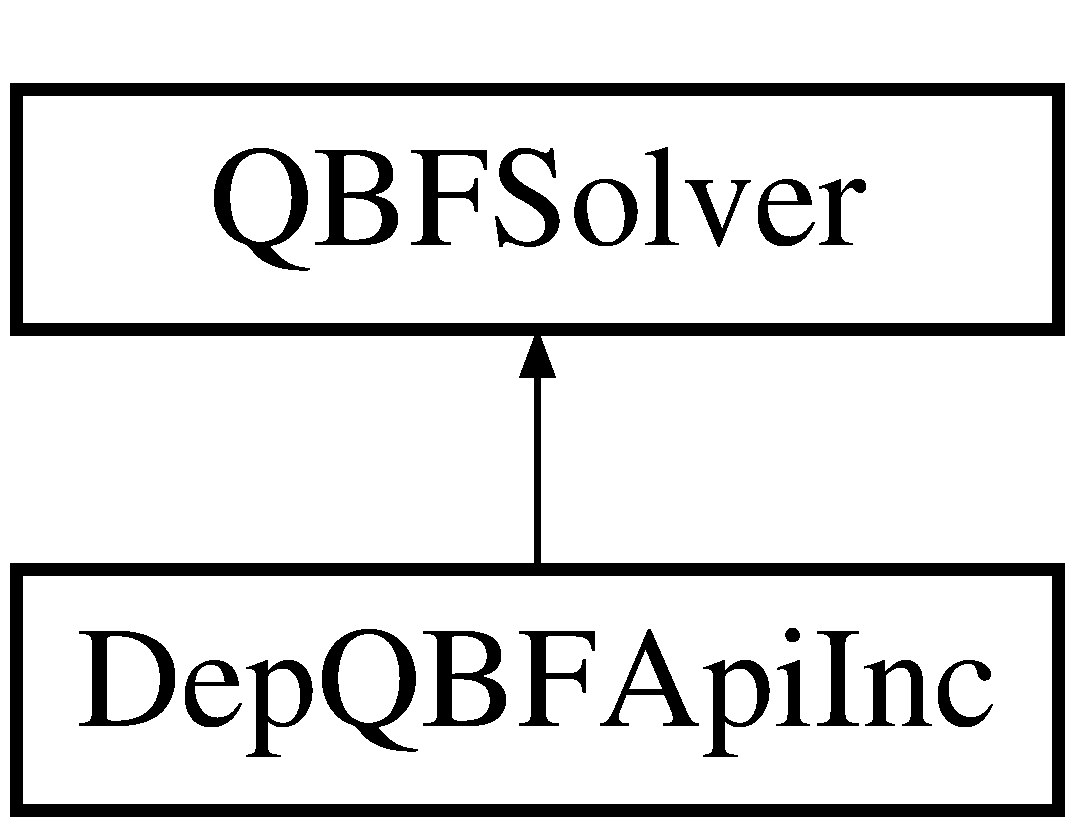
\includegraphics[height=2.000000cm]{classDepQBFApiInc}
\end{center}
\end{figure}
\subsection*{Public Types}
\begin{DoxyCompactItemize}
\item 
enum \hyperlink{classQBFSolver_ac091e263cb55286cc07b2451bcf4d3c7}{Quant} \{ \hyperlink{classQBFSolver_ac091e263cb55286cc07b2451bcf4d3c7a090ab4a5b262710ccd80e97d72f9a7b3}{E}, 
\hyperlink{classQBFSolver_ac091e263cb55286cc07b2451bcf4d3c7afd6518d5d985aa8346ac071e4c0d8ee0}{A}
 \}
\begin{DoxyCompactList}\small\item\em A type for the different kinds of quantifiers. \end{DoxyCompactList}\end{DoxyCompactItemize}
\subsection*{Public Member Functions}
\begin{DoxyCompactItemize}
\item 
\hyperlink{classDepQBFApiInc_a013e8e74c09c3bc36e795d3086f13abe}{Dep\-Q\-B\-F\-Api\-Inc} (bool use\-\_\-bloqqer=false)
\begin{DoxyCompactList}\small\item\em Constructor. \end{DoxyCompactList}\item 
virtual \hyperlink{classDepQBFApiInc_a0ccf94c512221ae643199c230228b3d6}{$\sim$\-Dep\-Q\-B\-F\-Api\-Inc} ()
\begin{DoxyCompactList}\small\item\em Destructor. \end{DoxyCompactList}\item 
virtual bool \hyperlink{classDepQBFApiInc_a7c99e11dd78c20aafb159c3633daae1d}{is\-Sat} (const vector$<$ pair$<$ \hyperlink{classVarInfo_a64d1da76cf84fe674e5fef9764ef11cf}{Var\-Info\-::\-Var\-Kind}, \hyperlink{classQBFSolver_ac091e263cb55286cc07b2451bcf4d3c7}{Quant} $>$ $>$ \&quantifier\-\_\-prefix, const \hyperlink{classCNF}{C\-N\-F} \&cnf)
\begin{DoxyCompactList}\small\item\em Checks if a given Q\-B\-F is satisfiable (with quantification over variable kinds). \end{DoxyCompactList}\item 
virtual bool \hyperlink{classDepQBFApiInc_a33426c8cfba9cfe5504bdf9c28f988a2}{is\-Sat} (const vector$<$ pair$<$ vector$<$ int $>$, \hyperlink{classQBFSolver_ac091e263cb55286cc07b2451bcf4d3c7}{Quant} $>$ $>$ \&quantifier\-\_\-prefix, const \hyperlink{classCNF}{C\-N\-F} \&cnf)
\begin{DoxyCompactList}\small\item\em Checks if a given Q\-B\-F is satisfiable (with quantification over variable sets). \end{DoxyCompactList}\item 
virtual bool \hyperlink{classDepQBFApiInc_a76c8046078bcd13fe864e1b8621ed6c3}{is\-Sat\-Model} (const vector$<$ pair$<$ \hyperlink{classVarInfo_a64d1da76cf84fe674e5fef9764ef11cf}{Var\-Info\-::\-Var\-Kind}, \hyperlink{classQBFSolver_ac091e263cb55286cc07b2451bcf4d3c7}{Quant} $>$ $>$ \&quantifier\-\_\-prefix, const \hyperlink{classCNF}{C\-N\-F} \&cnf, vector$<$ int $>$ \&model)
\begin{DoxyCompactList}\small\item\em Checks satisfiability and extracts a model (quantifying over variable kinds). \end{DoxyCompactList}\item 
virtual bool \hyperlink{classDepQBFApiInc_a61c1de56b115323863c326b248d10acb}{is\-Sat\-Model} (const vector$<$ pair$<$ vector$<$ int $>$, \hyperlink{classQBFSolver_ac091e263cb55286cc07b2451bcf4d3c7}{Quant} $>$ $>$ \&quantifier\-\_\-prefix, const \hyperlink{classCNF}{C\-N\-F} \&cnf, vector$<$ int $>$ \&model)
\begin{DoxyCompactList}\small\item\em Checks satisfiability and extracts a model (quantifying over variable sets). \end{DoxyCompactList}\item 
virtual void \hyperlink{classDepQBFApiInc_afdeb5e6df1be1c52ba79a993b47bebb5}{start\-Incremental\-Session} (const vector$<$ pair$<$ \hyperlink{classVarInfo_a64d1da76cf84fe674e5fef9764ef11cf}{Var\-Info\-::\-Var\-Kind}, \hyperlink{classQBFSolver_ac091e263cb55286cc07b2451bcf4d3c7}{Quant} $>$ $>$ \&quantifier\-\_\-prefix)
\begin{DoxyCompactList}\small\item\em Starts an 'incremental' session with a quantifier prefix over variable kinds. \end{DoxyCompactList}\item 
virtual void \hyperlink{classDepQBFApiInc_a7e465808e8b3a704e9c0f20a1ed802c2}{start\-Incremental\-Session} (const vector$<$ pair$<$ vector$<$ int $>$, \hyperlink{classQBFSolver_ac091e263cb55286cc07b2451bcf4d3c7}{Quant} $>$ $>$ \&quantifier\-\_\-prefix)
\begin{DoxyCompactList}\small\item\em Starts an 'incremental' session with a quantifier prefix over variable sets. \end{DoxyCompactList}\item 
virtual void \hyperlink{classDepQBFApiInc_a352b4620501803cc6a267d458ee9c57d}{clear\-Incremental\-Session} ()
\begin{DoxyCompactList}\small\item\em Closes a previously opened incremental session and frees all resources. \end{DoxyCompactList}\item 
virtual void \hyperlink{classDepQBFApiInc_af6eacf0be1c7f0f29eeb02fefa63f3f9}{inc\-Add\-C\-N\-F} (const \hyperlink{classCNF}{C\-N\-F} \&cnf)
\begin{DoxyCompactList}\small\item\em Adds (conjuncts) a new \hyperlink{classCNF}{C\-N\-F} to the current incremental session. \end{DoxyCompactList}\item 
virtual void \hyperlink{classDepQBFApiInc_a02a9240f178470cd4c31b6584827aa1e}{inc\-Add\-Clause} (const vector$<$ int $>$ \&clause)
\begin{DoxyCompactList}\small\item\em Adds (conjuncts) a new clause to the current incremental session. \end{DoxyCompactList}\item 
virtual void \hyperlink{classDepQBFApiInc_af2844ae0ef747e2c86c840547f220e8c}{inc\-Add\-Cube} (const vector$<$ int $>$ \&cube)
\begin{DoxyCompactList}\small\item\em Adds (conjuncts) a new cube to the current incremental session. \end{DoxyCompactList}\item 
virtual bool \hyperlink{classDepQBFApiInc_ad2050c686056005bb7a670d4789c2c46}{inc\-Is\-Sat} ()
\begin{DoxyCompactList}\small\item\em Checks if the Q\-B\-F in the current incremental session is satisfiable. \end{DoxyCompactList}\item 
virtual bool \hyperlink{classDepQBFApiInc_ae7eb8958812c2749700d73814a0e5be9}{inc\-Is\-Sat} (const vector$<$ int $>$ \&assumptions)
\begin{DoxyCompactList}\small\item\em Checks if the Q\-B\-F in the incremental session is satisfiable under assumptions. \end{DoxyCompactList}\item 
virtual bool \hyperlink{classDepQBFApiInc_aa359b68463922dd0b1d20bd0e187f0f3}{inc\-Is\-Sat\-Model\-Or\-Core} (const vector$<$ int $>$ \&assumptions, vector$<$ int $>$ \&model\-\_\-or\-\_\-core)
\begin{DoxyCompactList}\small\item\em Checks if the incremental session is satisfiable and computes a model or core. \end{DoxyCompactList}\end{DoxyCompactItemize}
\subsection*{Protected Member Functions}
\begin{DoxyCompactItemize}
\item 
void \hyperlink{classDepQBFApiInc_a91a61cebcf4b1518599129f963eab273}{init\-Bloqqer} (const vector$<$ pair$<$ \hyperlink{classVarInfo_a64d1da76cf84fe674e5fef9764ef11cf}{Var\-Info\-::\-Var\-Kind}, \hyperlink{classQBFSolver_ac091e263cb55286cc07b2451bcf4d3c7}{Quant} $>$ $>$ \&quantifier\-\_\-prefix, const \hyperlink{classCNF}{C\-N\-F} \&cnf)
\begin{DoxyCompactList}\small\item\em Initializes the pre-\/processor with a Q\-B\-F (quantifying over variable kinds). \end{DoxyCompactList}\item 
void \hyperlink{classDepQBFApiInc_a51de5d859a17257f1ca23f5ea8561223}{init\-Bloqqer} (const vector$<$ pair$<$ vector$<$ int $>$, \hyperlink{classQBFSolver_ac091e263cb55286cc07b2451bcf4d3c7}{Quant} $>$ $>$ \&quantifier\-\_\-prefix, const \hyperlink{classCNF}{C\-N\-F} \&cnf)
\begin{DoxyCompactList}\small\item\em Initializes the pre-\/processor with a Q\-B\-F (quantifying over variable sets). \end{DoxyCompactList}\item 
void \hyperlink{classDepQBFApiInc_a6cfb19ba94dfeb3058542381cf6165b9}{init\-Dep\-Q\-B\-F} (Q\-D\-P\-L\-L $\ast$solver, const vector$<$ pair$<$ \hyperlink{classVarInfo_a64d1da76cf84fe674e5fef9764ef11cf}{Var\-Info\-::\-Var\-Kind}, \hyperlink{classQBFSolver_ac091e263cb55286cc07b2451bcf4d3c7}{Quant} $>$ $>$ \&quantifier\-\_\-prefix, const \hyperlink{classCNF}{C\-N\-F} \&cnf)
\begin{DoxyCompactList}\small\item\em Initializes a Dep\-Q\-B\-F instance with a Q\-B\-F (quantifying over variable kinds). \end{DoxyCompactList}\item 
void \hyperlink{classDepQBFApiInc_adf3a9ce984ae61132ef1d493eeafcae8}{init\-Dep\-Q\-B\-F} (Q\-D\-P\-L\-L $\ast$solver, const vector$<$ pair$<$ vector$<$ int $>$, \hyperlink{classQBFSolver_ac091e263cb55286cc07b2451bcf4d3c7}{Quant} $>$ $>$ \&quantifier\-\_\-prefix, const \hyperlink{classCNF}{C\-N\-F} \&cnf)
\begin{DoxyCompactList}\small\item\em Initializes a Dep\-Q\-B\-F instance with a Q\-B\-F (quantifying over variable sets). \end{DoxyCompactList}\item 
void \hyperlink{classDepQBFApiInc_abc030c55a52ca69b8189b14865b26509}{extract\-Core} (Q\-D\-P\-L\-L $\ast$solver, vector$<$ int $>$ \&core)
\begin{DoxyCompactList}\small\item\em Extracts an unsatisfiable core after unsatisfiability has been shown. \end{DoxyCompactList}\item 
void \hyperlink{classDepQBFApiInc_a2488712feac9625909a0cabf9eb09d22}{debug\-Check\-Bloqqer\-Verdict} (int bloqqer\-\_\-verdict, const vector$<$ pair$<$ \hyperlink{classVarInfo_a64d1da76cf84fe674e5fef9764ef11cf}{Var\-Info\-::\-Var\-Kind}, \hyperlink{classQBFSolver_ac091e263cb55286cc07b2451bcf4d3c7}{Quant} $>$ $>$ \&quantifier\-\_\-prefix, const \hyperlink{classCNF}{C\-N\-F} \&cnf)
\begin{DoxyCompactList}\small\item\em A debug function to cross-\/check bloqqer verdicts (S\-A\-T or U\-N\-S\-A\-T). \end{DoxyCompactList}\item 
void \hyperlink{classDepQBFApiInc_a82d045afc3065ae73ee37b61753c1f78}{debug\-Check\-Bloqqer\-Verdict} (int bloqqer\-\_\-verdict, const vector$<$ pair$<$ vector$<$ int $>$, \hyperlink{classQBFSolver_ac091e263cb55286cc07b2451bcf4d3c7}{Quant} $>$ $>$ \&quantifier\-\_\-prefix, const \hyperlink{classCNF}{C\-N\-F} \&cnf)
\begin{DoxyCompactList}\small\item\em A debug function to cross-\/check bloqqer verdicts (S\-A\-T or U\-N\-S\-A\-T). \end{DoxyCompactList}\item 
void \hyperlink{classDepQBFApiInc_a4a43ca2a646a9ca9b13f5328b925be50}{debug\-Check\-Bloqqer\-Model} (const vector$<$ int $>$ \&model, const vector$<$ pair$<$ \hyperlink{classVarInfo_a64d1da76cf84fe674e5fef9764ef11cf}{Var\-Info\-::\-Var\-Kind}, \hyperlink{classQBFSolver_ac091e263cb55286cc07b2451bcf4d3c7}{Quant} $>$ $>$ \&quantifier\-\_\-prefix, const \hyperlink{classCNF}{C\-N\-F} \&cnf)
\begin{DoxyCompactList}\small\item\em A debug function to cross-\/check models produced by bloqqer. \end{DoxyCompactList}\item 
void \hyperlink{classDepQBFApiInc_adf1a4898f0a95bd6784a4f338be9170b}{debug\-Check\-Bloqqer\-Model} (const vector$<$ int $>$ \&model, const vector$<$ pair$<$ vector$<$ int $>$, \hyperlink{classQBFSolver_ac091e263cb55286cc07b2451bcf4d3c7}{Quant} $>$ $>$ \&quantifier\-\_\-prefix, const \hyperlink{classCNF}{C\-N\-F} \&cnf)
\begin{DoxyCompactList}\small\item\em A debug function to cross-\/check models produced by bloqqer. \end{DoxyCompactList}\end{DoxyCompactItemize}
\subsection*{Protected Attributes}
\begin{DoxyCompactItemize}
\item 
bool \hyperlink{classDepQBFApiInc_af02ebc9cd6d44dabef38211a0aa382e6}{use\-\_\-bloqqer\-\_\-}
\begin{DoxyCompactList}\small\item\em A flag indicating whether or not the pre-\/processor bloqqer should be used. \end{DoxyCompactList}\item 
bool \hyperlink{classDepQBFApiInc_a973cfad8d1464ceab22eab182332fe20}{min\-\_\-cores\-\_\-}
\begin{DoxyCompactList}\small\item\em A flag indicating whether or not unsatisfiable cores should be further minimized. \end{DoxyCompactList}\item 
Q\-D\-P\-L\-L $\ast$ \hyperlink{classDepQBFApiInc_ab1380371d12eb536493bfa8851ee7bc3}{inc\-\_\-solver\-\_\-}
\begin{DoxyCompactList}\small\item\em The solver instance to use in the incremental session. \end{DoxyCompactList}\item 
vector$<$ int $>$ \hyperlink{classDepQBFApiInc_a4dc19de8b66b9133906d7ef6b228e075}{inc\-\_\-model\-\_\-vars\-\_\-}
\begin{DoxyCompactList}\small\item\em The variables for which a satisfying assignment can be constructed. \end{DoxyCompactList}\end{DoxyCompactItemize}
\subsection*{Private Member Functions}
\begin{DoxyCompactItemize}
\item 
\hyperlink{classDepQBFApiInc_a1f6265470a8d137973acf9a3a8a41d64}{Dep\-Q\-B\-F\-Api\-Inc} (const \hyperlink{classDepQBFApiInc}{Dep\-Q\-B\-F\-Api\-Inc} \&other)
\begin{DoxyCompactList}\small\item\em Copy constructor. \end{DoxyCompactList}\item 
\hyperlink{classDepQBFApiInc}{Dep\-Q\-B\-F\-Api\-Inc} \& \hyperlink{classDepQBFApiInc_a29aebedc976f97274b83325e4ca73b96}{operator=} (const \hyperlink{classDepQBFApiInc}{Dep\-Q\-B\-F\-Api\-Inc} \&other)
\begin{DoxyCompactList}\small\item\em Assignment operator. \end{DoxyCompactList}\end{DoxyCompactItemize}


\subsection{Detailed Description}
Interfaces an experimental Dep\-Q\-B\-F-\/version via its A\-P\-I. 

This class represents an interface to an experimental version of the Q\-B\-F-\/solver Dep\-Q\-B\-F (see \href{https://github.com/lonsing/depqbf}{\tt https\-://github.\-com/lonsing/depqbf}). This version is not (yet) publicly available. In addition to the features of \hyperlink{classDepQBFApi}{Dep\-Q\-B\-F\-Api}, this interface to Dep\-Q\-B\-F can also compute unsatisfiable cores. Furthermore, it can use Dep\-Q\-B\-F incrementally in the sense that clauses that talk only about variables that are quantified existentially on the outermost quantifier block can be added without a need to restart the solver completely.

Otherwise, this class is equivalent to \hyperlink{classDepQBFApi}{Dep\-Q\-B\-F\-Api}.

\begin{DoxyNote}{Note}
This class is experimental. 
\end{DoxyNote}
\begin{DoxyAuthor}{Author}
Robert Koenighofer (\href{mailto:robert.koenighofer@iaik.tugraz.at}{\tt robert.\-koenighofer@iaik.\-tugraz.\-at}) 
\end{DoxyAuthor}
\begin{DoxyVersion}{Version}
1.\-0.\-0 
\end{DoxyVersion}


Definition at line 55 of file Dep\-Q\-B\-F\-Api\-Inc.\-h.



\subsection{Member Enumeration Documentation}
\hypertarget{classQBFSolver_ac091e263cb55286cc07b2451bcf4d3c7}{\index{Dep\-Q\-B\-F\-Api\-Inc@{Dep\-Q\-B\-F\-Api\-Inc}!Quant@{Quant}}
\index{Quant@{Quant}!DepQBFApiInc@{Dep\-Q\-B\-F\-Api\-Inc}}
\subsubsection[{Quant}]{\setlength{\rightskip}{0pt plus 5cm}enum {\bf Q\-B\-F\-Solver\-::\-Quant}\hspace{0.3cm}{\ttfamily [inherited]}}}\label{classQBFSolver_ac091e263cb55286cc07b2451bcf4d3c7}


A type for the different kinds of quantifiers. 

\begin{Desc}
\item[Enumerator\-: ]\par
\begin{description}
\index{E@{E}!Dep\-Q\-B\-F\-Api\-Inc@{Dep\-Q\-B\-F\-Api\-Inc}}\index{Dep\-Q\-B\-F\-Api\-Inc@{Dep\-Q\-B\-F\-Api\-Inc}!E@{E}}\item[{\em 
\hypertarget{classQBFSolver_ac091e263cb55286cc07b2451bcf4d3c7a090ab4a5b262710ccd80e97d72f9a7b3}{E}\label{classQBFSolver_ac091e263cb55286cc07b2451bcf4d3c7a090ab4a5b262710ccd80e97d72f9a7b3}
}]The value for existential quantification. \index{A@{A}!Dep\-Q\-B\-F\-Api\-Inc@{Dep\-Q\-B\-F\-Api\-Inc}}\index{Dep\-Q\-B\-F\-Api\-Inc@{Dep\-Q\-B\-F\-Api\-Inc}!A@{A}}\item[{\em 
\hypertarget{classQBFSolver_ac091e263cb55286cc07b2451bcf4d3c7afd6518d5d985aa8346ac071e4c0d8ee0}{A}\label{classQBFSolver_ac091e263cb55286cc07b2451bcf4d3c7afd6518d5d985aa8346ac071e4c0d8ee0}
}]The value for universal quantification. \end{description}
\end{Desc}



Definition at line 56 of file Q\-B\-F\-Solver.\-h.



\subsection{Constructor \& Destructor Documentation}
\hypertarget{classDepQBFApiInc_a013e8e74c09c3bc36e795d3086f13abe}{\index{Dep\-Q\-B\-F\-Api\-Inc@{Dep\-Q\-B\-F\-Api\-Inc}!Dep\-Q\-B\-F\-Api\-Inc@{Dep\-Q\-B\-F\-Api\-Inc}}
\index{Dep\-Q\-B\-F\-Api\-Inc@{Dep\-Q\-B\-F\-Api\-Inc}!DepQBFApiInc@{Dep\-Q\-B\-F\-Api\-Inc}}
\subsubsection[{Dep\-Q\-B\-F\-Api\-Inc}]{\setlength{\rightskip}{0pt plus 5cm}Dep\-Q\-B\-F\-Api\-Inc\-::\-Dep\-Q\-B\-F\-Api\-Inc (
\begin{DoxyParamCaption}
\item[{bool}]{use\-\_\-bloqqer = {\ttfamily false}}
\end{DoxyParamCaption}
)}}\label{classDepQBFApiInc_a013e8e74c09c3bc36e795d3086f13abe}


Constructor. 


\begin{DoxyParams}{Parameters}
{\em use\-\_\-bloqqer} & True if bloqqer should be used as pre-\/processor, false if no pre-\/processing should be used. If this parameter is omitted, no pre-\/processing is used. \\
\hline
\end{DoxyParams}


Definition at line 42 of file Dep\-Q\-B\-F\-Api\-Inc.\-cpp.

\hypertarget{classDepQBFApiInc_a0ccf94c512221ae643199c230228b3d6}{\index{Dep\-Q\-B\-F\-Api\-Inc@{Dep\-Q\-B\-F\-Api\-Inc}!$\sim$\-Dep\-Q\-B\-F\-Api\-Inc@{$\sim$\-Dep\-Q\-B\-F\-Api\-Inc}}
\index{$\sim$\-Dep\-Q\-B\-F\-Api\-Inc@{$\sim$\-Dep\-Q\-B\-F\-Api\-Inc}!DepQBFApiInc@{Dep\-Q\-B\-F\-Api\-Inc}}
\subsubsection[{$\sim$\-Dep\-Q\-B\-F\-Api\-Inc}]{\setlength{\rightskip}{0pt plus 5cm}Dep\-Q\-B\-F\-Api\-Inc\-::$\sim$\-Dep\-Q\-B\-F\-Api\-Inc (
\begin{DoxyParamCaption}
{}
\end{DoxyParamCaption}
)\hspace{0.3cm}{\ttfamily [virtual]}}}\label{classDepQBFApiInc_a0ccf94c512221ae643199c230228b3d6}


Destructor. 



Definition at line 51 of file Dep\-Q\-B\-F\-Api\-Inc.\-cpp.



References clear\-Incremental\-Session().

\hypertarget{classDepQBFApiInc_a1f6265470a8d137973acf9a3a8a41d64}{\index{Dep\-Q\-B\-F\-Api\-Inc@{Dep\-Q\-B\-F\-Api\-Inc}!Dep\-Q\-B\-F\-Api\-Inc@{Dep\-Q\-B\-F\-Api\-Inc}}
\index{Dep\-Q\-B\-F\-Api\-Inc@{Dep\-Q\-B\-F\-Api\-Inc}!DepQBFApiInc@{Dep\-Q\-B\-F\-Api\-Inc}}
\subsubsection[{Dep\-Q\-B\-F\-Api\-Inc}]{\setlength{\rightskip}{0pt plus 5cm}Dep\-Q\-B\-F\-Api\-Inc\-::\-Dep\-Q\-B\-F\-Api\-Inc (
\begin{DoxyParamCaption}
\item[{const {\bf Dep\-Q\-B\-F\-Api\-Inc} \&}]{other}
\end{DoxyParamCaption}
)\hspace{0.3cm}{\ttfamily [private]}}}\label{classDepQBFApiInc_a1f6265470a8d137973acf9a3a8a41d64}


Copy constructor. 

The copy constructor is disabled (set private) and not implemented.


\begin{DoxyParams}{Parameters}
{\em other} & The source for creating the copy. \\
\hline
\end{DoxyParams}


\subsection{Member Function Documentation}
\hypertarget{classDepQBFApiInc_a352b4620501803cc6a267d458ee9c57d}{\index{Dep\-Q\-B\-F\-Api\-Inc@{Dep\-Q\-B\-F\-Api\-Inc}!clear\-Incremental\-Session@{clear\-Incremental\-Session}}
\index{clear\-Incremental\-Session@{clear\-Incremental\-Session}!DepQBFApiInc@{Dep\-Q\-B\-F\-Api\-Inc}}
\subsubsection[{clear\-Incremental\-Session}]{\setlength{\rightskip}{0pt plus 5cm}void Dep\-Q\-B\-F\-Api\-Inc\-::clear\-Incremental\-Session (
\begin{DoxyParamCaption}
{}
\end{DoxyParamCaption}
)\hspace{0.3cm}{\ttfamily [virtual]}}}\label{classDepQBFApiInc_a352b4620501803cc6a267d458ee9c57d}


Closes a previously opened incremental session and frees all resources. 

If no incremental session is open, then this method has no effect at all. 

Definition at line 370 of file Dep\-Q\-B\-F\-Api\-Inc.\-cpp.



References inc\-\_\-model\-\_\-vars\-\_\-, inc\-\_\-solver\-\_\-, and M\-A\-S\-S\-E\-R\-T.



Referenced by $\sim$\-Dep\-Q\-B\-F\-Api\-Inc().

\hypertarget{classDepQBFApiInc_a4a43ca2a646a9ca9b13f5328b925be50}{\index{Dep\-Q\-B\-F\-Api\-Inc@{Dep\-Q\-B\-F\-Api\-Inc}!debug\-Check\-Bloqqer\-Model@{debug\-Check\-Bloqqer\-Model}}
\index{debug\-Check\-Bloqqer\-Model@{debug\-Check\-Bloqqer\-Model}!DepQBFApiInc@{Dep\-Q\-B\-F\-Api\-Inc}}
\subsubsection[{debug\-Check\-Bloqqer\-Model}]{\setlength{\rightskip}{0pt plus 5cm}void Dep\-Q\-B\-F\-Api\-Inc\-::debug\-Check\-Bloqqer\-Model (
\begin{DoxyParamCaption}
\item[{const vector$<$ int $>$ \&}]{model, }
\item[{const vector$<$ pair$<$ {\bf Var\-Info\-::\-Var\-Kind}, {\bf Quant} $>$ $>$ \&}]{quantifier\-\_\-prefix, }
\item[{const {\bf C\-N\-F} \&}]{cnf}
\end{DoxyParamCaption}
)\hspace{0.3cm}{\ttfamily [protected]}}}\label{classDepQBFApiInc_a4a43ca2a646a9ca9b13f5328b925be50}


A debug function to cross-\/check models produced by bloqqer. 

Dep\-Q\-B\-F without preprocessing is used to check if the model found by bloqqer indeed satisfies the Q\-B\-F. This method is used to debug bloqqer.


\begin{DoxyParams}{Parameters}
{\em model} & The satisfying assignment found by bloqqer. Negated variables in the vector are F\-A\-L\-S\-E, unnegated ones are T\-R\-U\-E. \\
\hline
{\em quantifier\-\_\-prefix} & The quantifier prefix as a vector of pairs. vector\mbox{[}0\mbox{]} is the leftmost (i.\-e., outermost) quantifier block. The pairs in the quantifier\-\_\-prefix assign an existential or universal quantifier to every kind of variable that occurs in the cnf. \\
\hline
{\em cnf} & A Boolean formula in \hyperlink{classCNF}{C\-N\-F}. \\
\hline
\end{DoxyParams}


Definition at line 744 of file Dep\-Q\-B\-F\-Api\-Inc.\-cpp.



References C\-N\-F\-::add\-Cube(), Utils\-::debug\-Print(), Ext\-Q\-B\-F\-Solver\-::dump\-Q\-B\-F(), Var\-Manager\-::get\-Vars\-Of\-Type(), Var\-Manager\-::instance(), is\-Sat(), L\-\_\-\-E\-R\-R, and M\-A\-S\-S\-E\-R\-T.

\hypertarget{classDepQBFApiInc_adf1a4898f0a95bd6784a4f338be9170b}{\index{Dep\-Q\-B\-F\-Api\-Inc@{Dep\-Q\-B\-F\-Api\-Inc}!debug\-Check\-Bloqqer\-Model@{debug\-Check\-Bloqqer\-Model}}
\index{debug\-Check\-Bloqqer\-Model@{debug\-Check\-Bloqqer\-Model}!DepQBFApiInc@{Dep\-Q\-B\-F\-Api\-Inc}}
\subsubsection[{debug\-Check\-Bloqqer\-Model}]{\setlength{\rightskip}{0pt plus 5cm}void Dep\-Q\-B\-F\-Api\-Inc\-::debug\-Check\-Bloqqer\-Model (
\begin{DoxyParamCaption}
\item[{const vector$<$ int $>$ \&}]{model, }
\item[{const vector$<$ pair$<$ vector$<$ int $>$, {\bf Quant} $>$ $>$ \&}]{quantifier\-\_\-prefix, }
\item[{const {\bf C\-N\-F} \&}]{cnf}
\end{DoxyParamCaption}
)\hspace{0.3cm}{\ttfamily [protected]}}}\label{classDepQBFApiInc_adf1a4898f0a95bd6784a4f338be9170b}


A debug function to cross-\/check models produced by bloqqer. 

Dep\-Q\-B\-F without preprocessing is used to check if the model found by bloqqer indeed satisfies the Q\-B\-F. This method is used to debug bloqqer.


\begin{DoxyParams}{Parameters}
{\em model} & The satisfying assignment found by bloqqer. Negated variables in the vector are F\-A\-L\-S\-E, unnegated ones are T\-R\-U\-E. \\
\hline
{\em quantifier\-\_\-prefix} & The quantifier prefix as a vector of pairs. vector\mbox{[}0\mbox{]} is the leftmost (i.\-e., outermost) quantifier block. The pairs in the quantifier\-\_\-prefix assign an existential or universal quantifier to different sets of variables occurring in the cnf. \\
\hline
{\em cnf} & A Boolean formula in \hyperlink{classCNF}{C\-N\-F}. \\
\hline
\end{DoxyParams}


Definition at line 791 of file Dep\-Q\-B\-F\-Api\-Inc.\-cpp.



References C\-N\-F\-::add\-Cube(), Utils\-::debug\-Print(), Ext\-Q\-B\-F\-Solver\-::dump\-Q\-B\-F(), is\-Sat(), L\-\_\-\-E\-R\-R, and M\-A\-S\-S\-E\-R\-T.

\hypertarget{classDepQBFApiInc_a2488712feac9625909a0cabf9eb09d22}{\index{Dep\-Q\-B\-F\-Api\-Inc@{Dep\-Q\-B\-F\-Api\-Inc}!debug\-Check\-Bloqqer\-Verdict@{debug\-Check\-Bloqqer\-Verdict}}
\index{debug\-Check\-Bloqqer\-Verdict@{debug\-Check\-Bloqqer\-Verdict}!DepQBFApiInc@{Dep\-Q\-B\-F\-Api\-Inc}}
\subsubsection[{debug\-Check\-Bloqqer\-Verdict}]{\setlength{\rightskip}{0pt plus 5cm}void Dep\-Q\-B\-F\-Api\-Inc\-::debug\-Check\-Bloqqer\-Verdict (
\begin{DoxyParamCaption}
\item[{int}]{bloqqer\-\_\-verdict, }
\item[{const vector$<$ pair$<$ {\bf Var\-Info\-::\-Var\-Kind}, {\bf Quant} $>$ $>$ \&}]{quantifier\-\_\-prefix, }
\item[{const {\bf C\-N\-F} \&}]{cnf}
\end{DoxyParamCaption}
)\hspace{0.3cm}{\ttfamily [protected]}}}\label{classDepQBFApiInc_a2488712feac9625909a0cabf9eb09d22}


A debug function to cross-\/check bloqqer verdicts (S\-A\-T or U\-N\-S\-A\-T). 

The Q\-B\-F is also solved with Dep\-Q\-B\-F without pre-\/processing and the two verdicts are compared. This method is used to debug bloqqer.


\begin{DoxyParams}{Parameters}
{\em bloqqer\-\_\-verdict} & The result returned by bloqqer. The value 10 means S\-A\-T, the value 20 means U\-N\-S\-A\-T. \\
\hline
{\em quantifier\-\_\-prefix} & The quantifier prefix as a vector of pairs. vector\mbox{[}0\mbox{]} is the leftmost (i.\-e., outermost) quantifier block. The pairs in the quantifier\-\_\-prefix assign an existential or universal quantifier to every kind of variable that occurs in the cnf. \\
\hline
{\em cnf} & A Boolean formula in \hyperlink{classCNF}{C\-N\-F}. \\
\hline
\end{DoxyParams}


Definition at line 686 of file Dep\-Q\-B\-F\-Api\-Inc.\-cpp.



References Ext\-Q\-B\-F\-Solver\-::dump\-Q\-B\-F(), is\-Sat(), L\-\_\-\-E\-R\-R, and M\-A\-S\-S\-E\-R\-T.



Referenced by is\-Sat\-Model().

\hypertarget{classDepQBFApiInc_a82d045afc3065ae73ee37b61753c1f78}{\index{Dep\-Q\-B\-F\-Api\-Inc@{Dep\-Q\-B\-F\-Api\-Inc}!debug\-Check\-Bloqqer\-Verdict@{debug\-Check\-Bloqqer\-Verdict}}
\index{debug\-Check\-Bloqqer\-Verdict@{debug\-Check\-Bloqqer\-Verdict}!DepQBFApiInc@{Dep\-Q\-B\-F\-Api\-Inc}}
\subsubsection[{debug\-Check\-Bloqqer\-Verdict}]{\setlength{\rightskip}{0pt plus 5cm}void Dep\-Q\-B\-F\-Api\-Inc\-::debug\-Check\-Bloqqer\-Verdict (
\begin{DoxyParamCaption}
\item[{int}]{bloqqer\-\_\-verdict, }
\item[{const vector$<$ pair$<$ vector$<$ int $>$, {\bf Quant} $>$ $>$ \&}]{quantifier\-\_\-prefix, }
\item[{const {\bf C\-N\-F} \&}]{cnf}
\end{DoxyParamCaption}
)\hspace{0.3cm}{\ttfamily [protected]}}}\label{classDepQBFApiInc_a82d045afc3065ae73ee37b61753c1f78}


A debug function to cross-\/check bloqqer verdicts (S\-A\-T or U\-N\-S\-A\-T). 

The Q\-B\-F is also solved with Dep\-Q\-B\-F without pre-\/processing and the two verdicts are compared. This method is used to debug bloqqer.


\begin{DoxyParams}{Parameters}
{\em bloqqer\-\_\-verdict} & The result returned by bloqqer. The value 10 means S\-A\-T, the value 20 means U\-N\-S\-A\-T. \\
\hline
{\em quantifier\-\_\-prefix} & The quantifier prefix as a vector of pairs. vector\mbox{[}0\mbox{]} is the leftmost (i.\-e., outermost) quantifier block. The pairs in the quantifier\-\_\-prefix assign an existential or universal quantifier to different sets of variables occurring in the cnf. \\
\hline
{\em cnf} & A Boolean formula in \hyperlink{classCNF}{C\-N\-F}. \\
\hline
\end{DoxyParams}


Definition at line 715 of file Dep\-Q\-B\-F\-Api\-Inc.\-cpp.



References Ext\-Q\-B\-F\-Solver\-::dump\-Q\-B\-F(), is\-Sat(), L\-\_\-\-E\-R\-R, and M\-A\-S\-S\-E\-R\-T.

\hypertarget{classDepQBFApiInc_abc030c55a52ca69b8189b14865b26509}{\index{Dep\-Q\-B\-F\-Api\-Inc@{Dep\-Q\-B\-F\-Api\-Inc}!extract\-Core@{extract\-Core}}
\index{extract\-Core@{extract\-Core}!DepQBFApiInc@{Dep\-Q\-B\-F\-Api\-Inc}}
\subsubsection[{extract\-Core}]{\setlength{\rightskip}{0pt plus 5cm}void Dep\-Q\-B\-F\-Api\-Inc\-::extract\-Core (
\begin{DoxyParamCaption}
\item[{Q\-D\-P\-L\-L $\ast$}]{solver, }
\item[{vector$<$ int $>$ \&}]{core}
\end{DoxyParamCaption}
)\hspace{0.3cm}{\ttfamily [protected]}}}\label{classDepQBFApiInc_abc030c55a52ca69b8189b14865b26509}


Extracts an unsatisfiable core after unsatisfiability has been shown. 


\begin{DoxyParams}{Parameters}
{\em solver} & The Dep\-Q\-B\-F solver instance to extract the core from. \\
\hline
{\em core} & The vector into which the resulting unsatisfiable core will be stored. It is a subset of the used assumptions. \\
\hline
\end{DoxyParams}


Definition at line 638 of file Dep\-Q\-B\-F\-Api\-Inc.\-cpp.



References M\-A\-S\-S\-E\-R\-T, min\-\_\-cores\-\_\-, Utils\-::randomize(), and Utils\-::remove().



Referenced by inc\-Is\-Sat\-Model\-Or\-Core().

\hypertarget{classDepQBFApiInc_a02a9240f178470cd4c31b6584827aa1e}{\index{Dep\-Q\-B\-F\-Api\-Inc@{Dep\-Q\-B\-F\-Api\-Inc}!inc\-Add\-Clause@{inc\-Add\-Clause}}
\index{inc\-Add\-Clause@{inc\-Add\-Clause}!DepQBFApiInc@{Dep\-Q\-B\-F\-Api\-Inc}}
\subsubsection[{inc\-Add\-Clause}]{\setlength{\rightskip}{0pt plus 5cm}void Dep\-Q\-B\-F\-Api\-Inc\-::inc\-Add\-Clause (
\begin{DoxyParamCaption}
\item[{const vector$<$ int $>$ \&}]{clause}
\end{DoxyParamCaption}
)\hspace{0.3cm}{\ttfamily [virtual]}}}\label{classDepQBFApiInc_a02a9240f178470cd4c31b6584827aa1e}


Adds (conjuncts) a new clause to the current incremental session. 

\begin{DoxyPrecond}{Precondition}
\hyperlink{classDepQBFApiInc_afdeb5e6df1be1c52ba79a993b47bebb5}{start\-Incremental\-Session() } must have been called before. 
\end{DoxyPrecond}

\begin{DoxyParams}{Parameters}
{\em clause} & The clause which shall be conjuncted to the \hyperlink{classCNF}{C\-N\-F} in the currently open incremental session. \\
\hline
\end{DoxyParams}


Definition at line 402 of file Dep\-Q\-B\-F\-Api\-Inc.\-cpp.



References inc\-\_\-solver\-\_\-, and M\-A\-S\-S\-E\-R\-T.



Referenced by Learn\-Synth\-Q\-B\-F\-Inc\-::compute\-Winning\-Region\-All(), and Learn\-Synth\-Q\-B\-F\-Inc\-::compute\-Winning\-Region\-One().

\hypertarget{classDepQBFApiInc_af6eacf0be1c7f0f29eeb02fefa63f3f9}{\index{Dep\-Q\-B\-F\-Api\-Inc@{Dep\-Q\-B\-F\-Api\-Inc}!inc\-Add\-C\-N\-F@{inc\-Add\-C\-N\-F}}
\index{inc\-Add\-C\-N\-F@{inc\-Add\-C\-N\-F}!DepQBFApiInc@{Dep\-Q\-B\-F\-Api\-Inc}}
\subsubsection[{inc\-Add\-C\-N\-F}]{\setlength{\rightskip}{0pt plus 5cm}void Dep\-Q\-B\-F\-Api\-Inc\-::inc\-Add\-C\-N\-F (
\begin{DoxyParamCaption}
\item[{const {\bf C\-N\-F} \&}]{cnf}
\end{DoxyParamCaption}
)\hspace{0.3cm}{\ttfamily [virtual]}}}\label{classDepQBFApiInc_af6eacf0be1c7f0f29eeb02fefa63f3f9}


Adds (conjuncts) a new \hyperlink{classCNF}{C\-N\-F} to the current incremental session. 

\begin{DoxyPrecond}{Precondition}
\hyperlink{classDepQBFApiInc_afdeb5e6df1be1c52ba79a993b47bebb5}{start\-Incremental\-Session() } must have been called before. 
\end{DoxyPrecond}

\begin{DoxyParams}{Parameters}
{\em cnf} & A Boolean formula in \hyperlink{classCNF}{C\-N\-F}. It is conjuncted to the \hyperlink{classCNF}{C\-N\-F} in the currently open incremental session. \\
\hline
\end{DoxyParams}


Definition at line 385 of file Dep\-Q\-B\-F\-Api\-Inc.\-cpp.



References C\-N\-F\-::get\-Clauses(), inc\-\_\-solver\-\_\-, and M\-A\-S\-S\-E\-R\-T.



Referenced by Learn\-Synth\-Q\-B\-F\-Inc\-::compute\-All\-Blocking\-Clauses(), Learn\-Synth\-Q\-B\-F\-Inc\-::compute\-Blocking\-Clause(), Learn\-Synth\-Q\-B\-F\-Inc\-::compute\-Winning\-Region\-All(), Learn\-Synth\-Q\-B\-F\-Inc\-::compute\-Winning\-Region\-One(), and Learn\-Synth\-Q\-B\-F\-Inc\-::reduce\-Existing\-Clauses().

\hypertarget{classDepQBFApiInc_af2844ae0ef747e2c86c840547f220e8c}{\index{Dep\-Q\-B\-F\-Api\-Inc@{Dep\-Q\-B\-F\-Api\-Inc}!inc\-Add\-Cube@{inc\-Add\-Cube}}
\index{inc\-Add\-Cube@{inc\-Add\-Cube}!DepQBFApiInc@{Dep\-Q\-B\-F\-Api\-Inc}}
\subsubsection[{inc\-Add\-Cube}]{\setlength{\rightskip}{0pt plus 5cm}void Dep\-Q\-B\-F\-Api\-Inc\-::inc\-Add\-Cube (
\begin{DoxyParamCaption}
\item[{const vector$<$ int $>$ \&}]{cube}
\end{DoxyParamCaption}
)\hspace{0.3cm}{\ttfamily [virtual]}}}\label{classDepQBFApiInc_af2844ae0ef747e2c86c840547f220e8c}


Adds (conjuncts) a new cube to the current incremental session. 

\begin{DoxyPrecond}{Precondition}
\hyperlink{classDepQBFApiInc_afdeb5e6df1be1c52ba79a993b47bebb5}{start\-Incremental\-Session() } must have been called before. 
\end{DoxyPrecond}

\begin{DoxyParams}{Parameters}
{\em cube} & The cube which shall be conjuncted to the \hyperlink{classCNF}{C\-N\-F} in the currently open incremental session. All literals of the cube are added as unit clauses to the \hyperlink{classCNF}{C\-N\-F} of the currently open session. \\
\hline
\end{DoxyParams}


Definition at line 415 of file Dep\-Q\-B\-F\-Api\-Inc.\-cpp.



References inc\-\_\-solver\-\_\-, and M\-A\-S\-S\-E\-R\-T.

\hypertarget{classDepQBFApiInc_ad2050c686056005bb7a670d4789c2c46}{\index{Dep\-Q\-B\-F\-Api\-Inc@{Dep\-Q\-B\-F\-Api\-Inc}!inc\-Is\-Sat@{inc\-Is\-Sat}}
\index{inc\-Is\-Sat@{inc\-Is\-Sat}!DepQBFApiInc@{Dep\-Q\-B\-F\-Api\-Inc}}
\subsubsection[{inc\-Is\-Sat}]{\setlength{\rightskip}{0pt plus 5cm}bool Dep\-Q\-B\-F\-Api\-Inc\-::inc\-Is\-Sat (
\begin{DoxyParamCaption}
{}
\end{DoxyParamCaption}
)\hspace{0.3cm}{\ttfamily [virtual]}}}\label{classDepQBFApiInc_ad2050c686056005bb7a670d4789c2c46}


Checks if the Q\-B\-F in the current incremental session is satisfiable. 

\begin{DoxyReturn}{Returns}
True if the Q\-B\-F in the current incremental session is satisfiable, false otherwise. 
\end{DoxyReturn}


Definition at line 430 of file Dep\-Q\-B\-F\-Api\-Inc.\-cpp.



References inc\-\_\-solver\-\_\-, and M\-A\-S\-S\-E\-R\-T.

\hypertarget{classDepQBFApiInc_ae7eb8958812c2749700d73814a0e5be9}{\index{Dep\-Q\-B\-F\-Api\-Inc@{Dep\-Q\-B\-F\-Api\-Inc}!inc\-Is\-Sat@{inc\-Is\-Sat}}
\index{inc\-Is\-Sat@{inc\-Is\-Sat}!DepQBFApiInc@{Dep\-Q\-B\-F\-Api\-Inc}}
\subsubsection[{inc\-Is\-Sat}]{\setlength{\rightskip}{0pt plus 5cm}bool Dep\-Q\-B\-F\-Api\-Inc\-::inc\-Is\-Sat (
\begin{DoxyParamCaption}
\item[{const vector$<$ int $>$ \&}]{assumptions}
\end{DoxyParamCaption}
)\hspace{0.3cm}{\ttfamily [virtual]}}}\label{classDepQBFApiInc_ae7eb8958812c2749700d73814a0e5be9}


Checks if the Q\-B\-F in the incremental session is satisfiable under assumptions. 


\begin{DoxyParams}{Parameters}
{\em assumptions} & The assumptions under which the Q\-B\-F in the current incremental session should be solved. The assumptions are interpreted as a cube of literals. Every literal is added temporarily as a unit clause to the Q\-B\-F. \\
\hline
\end{DoxyParams}
\begin{DoxyReturn}{Returns}
True if the Q\-B\-F in the current incremental session is satisfiable under the assumptions, false otherwise. 
\end{DoxyReturn}


Definition at line 447 of file Dep\-Q\-B\-F\-Api\-Inc.\-cpp.



References inc\-\_\-solver\-\_\-, and M\-A\-S\-S\-E\-R\-T.

\hypertarget{classDepQBFApiInc_aa359b68463922dd0b1d20bd0e187f0f3}{\index{Dep\-Q\-B\-F\-Api\-Inc@{Dep\-Q\-B\-F\-Api\-Inc}!inc\-Is\-Sat\-Model\-Or\-Core@{inc\-Is\-Sat\-Model\-Or\-Core}}
\index{inc\-Is\-Sat\-Model\-Or\-Core@{inc\-Is\-Sat\-Model\-Or\-Core}!DepQBFApiInc@{Dep\-Q\-B\-F\-Api\-Inc}}
\subsubsection[{inc\-Is\-Sat\-Model\-Or\-Core}]{\setlength{\rightskip}{0pt plus 5cm}bool Dep\-Q\-B\-F\-Api\-Inc\-::inc\-Is\-Sat\-Model\-Or\-Core (
\begin{DoxyParamCaption}
\item[{const vector$<$ int $>$ \&}]{assumptions, }
\item[{vector$<$ int $>$ \&}]{model\-\_\-or\-\_\-core}
\end{DoxyParamCaption}
)\hspace{0.3cm}{\ttfamily [virtual]}}}\label{classDepQBFApiInc_aa359b68463922dd0b1d20bd0e187f0f3}


Checks if the incremental session is satisfiable and computes a model or core. 

This method first checks if the Q\-B\-F in the incremental session is satisfiable under a given set of assumptions. If yes, then a satisfying assignment for the variables quantified existentially on the outermost level is computed. Otherwise, an unsatisfiable core is computed. An unsatisfiable core is a subset of the assumptions under which the Q\-B\-F is still unsatisfiable.


\begin{DoxyParams}{Parameters}
{\em assumptions} & The assumptions under which the Q\-B\-F in the current incremental session should be solved. The assumptions are interpreted as a cube of literals. Every literal is added temporarily as a unit clause to the Q\-B\-F. \\
\hline
{\em model\-\_\-or\-\_\-core} & The vector into which the resulting model or core will be stored. In case of satisfiability a satisfying assignment (a cube of literals; negated ones are false, unnegated ones are true) is stored in this vector. Otherwise, if this method returns false, a subset of the passed assumptions is stored in this vector. \\
\hline
\end{DoxyParams}
\begin{DoxyReturn}{Returns}
True if the Q\-B\-F in the current incremental session is satisfiable under the assumptions, false otherwise. 
\end{DoxyReturn}


Definition at line 466 of file Dep\-Q\-B\-F\-Api\-Inc.\-cpp.



References extract\-Core(), inc\-\_\-model\-\_\-vars\-\_\-, inc\-\_\-solver\-\_\-, and M\-A\-S\-S\-E\-R\-T.



Referenced by Learn\-Synth\-Q\-B\-F\-Inc\-::compute\-Counterexample\-Q\-B\-F(), and Learn\-Synth\-Q\-B\-F\-Inc\-::generalize\-Counterexample().

\hypertarget{classDepQBFApiInc_a91a61cebcf4b1518599129f963eab273}{\index{Dep\-Q\-B\-F\-Api\-Inc@{Dep\-Q\-B\-F\-Api\-Inc}!init\-Bloqqer@{init\-Bloqqer}}
\index{init\-Bloqqer@{init\-Bloqqer}!DepQBFApiInc@{Dep\-Q\-B\-F\-Api\-Inc}}
\subsubsection[{init\-Bloqqer}]{\setlength{\rightskip}{0pt plus 5cm}void Dep\-Q\-B\-F\-Api\-Inc\-::init\-Bloqqer (
\begin{DoxyParamCaption}
\item[{const vector$<$ pair$<$ {\bf Var\-Info\-::\-Var\-Kind}, {\bf Quant} $>$ $>$ \&}]{quantifier\-\_\-prefix, }
\item[{const {\bf C\-N\-F} \&}]{cnf}
\end{DoxyParamCaption}
)\hspace{0.3cm}{\ttfamily [protected]}}}\label{classDepQBFApiInc_a91a61cebcf4b1518599129f963eab273}


Initializes the pre-\/processor with a Q\-B\-F (quantifying over variable kinds). 


\begin{DoxyParams}{Parameters}
{\em quantifier\-\_\-prefix} & The quantifier prefix as a vector of pairs. vector\mbox{[}0\mbox{]} is the leftmost (i.\-e., outermost) quantifier block. The pairs in the quantifier\-\_\-prefix assign an existential or universal quantifier to every kind of variable that occurs in the cnf. \\
\hline
{\em cnf} & A Boolean formula in \hyperlink{classCNF}{C\-N\-F}. \\
\hline
\end{DoxyParams}


Definition at line 511 of file Dep\-Q\-B\-F\-Api\-Inc.\-cpp.



References Q\-B\-F\-Solver\-::\-E, C\-N\-F\-::get\-Clauses(), Var\-Manager\-::get\-Max\-C\-N\-F\-Var(), C\-N\-F\-::get\-Nr\-Of\-Clauses(), Var\-Manager\-::get\-Vars\-Of\-Type(), and Var\-Manager\-::instance().



Referenced by is\-Sat(), and is\-Sat\-Model().

\hypertarget{classDepQBFApiInc_a51de5d859a17257f1ca23f5ea8561223}{\index{Dep\-Q\-B\-F\-Api\-Inc@{Dep\-Q\-B\-F\-Api\-Inc}!init\-Bloqqer@{init\-Bloqqer}}
\index{init\-Bloqqer@{init\-Bloqqer}!DepQBFApiInc@{Dep\-Q\-B\-F\-Api\-Inc}}
\subsubsection[{init\-Bloqqer}]{\setlength{\rightskip}{0pt plus 5cm}void Dep\-Q\-B\-F\-Api\-Inc\-::init\-Bloqqer (
\begin{DoxyParamCaption}
\item[{const vector$<$ pair$<$ vector$<$ int $>$, {\bf Quant} $>$ $>$ \&}]{quantifier\-\_\-prefix, }
\item[{const {\bf C\-N\-F} \&}]{cnf}
\end{DoxyParamCaption}
)\hspace{0.3cm}{\ttfamily [protected]}}}\label{classDepQBFApiInc_a51de5d859a17257f1ca23f5ea8561223}


Initializes the pre-\/processor with a Q\-B\-F (quantifying over variable sets). 


\begin{DoxyParams}{Parameters}
{\em quantifier\-\_\-prefix} & The quantifier prefix as a vector of pairs. vector\mbox{[}0\mbox{]} is the leftmost (i.\-e., outermost) quantifier block. The pairs in the quantifier\-\_\-prefix assign an existential or universal quantifier to different sets of variables occurring in the cnf. \\
\hline
{\em cnf} & A Boolean formula in \hyperlink{classCNF}{C\-N\-F}. \\
\hline
\end{DoxyParams}


Definition at line 539 of file Dep\-Q\-B\-F\-Api\-Inc.\-cpp.



References Q\-B\-F\-Solver\-::\-E, C\-N\-F\-::get\-Clauses(), and C\-N\-F\-::get\-Nr\-Of\-Clauses().

\hypertarget{classDepQBFApiInc_a6cfb19ba94dfeb3058542381cf6165b9}{\index{Dep\-Q\-B\-F\-Api\-Inc@{Dep\-Q\-B\-F\-Api\-Inc}!init\-Dep\-Q\-B\-F@{init\-Dep\-Q\-B\-F}}
\index{init\-Dep\-Q\-B\-F@{init\-Dep\-Q\-B\-F}!DepQBFApiInc@{Dep\-Q\-B\-F\-Api\-Inc}}
\subsubsection[{init\-Dep\-Q\-B\-F}]{\setlength{\rightskip}{0pt plus 5cm}void Dep\-Q\-B\-F\-Api\-Inc\-::init\-Dep\-Q\-B\-F (
\begin{DoxyParamCaption}
\item[{Q\-D\-P\-L\-L $\ast$}]{solver, }
\item[{const vector$<$ pair$<$ {\bf Var\-Info\-::\-Var\-Kind}, {\bf Quant} $>$ $>$ \&}]{quantifier\-\_\-prefix, }
\item[{const {\bf C\-N\-F} \&}]{cnf}
\end{DoxyParamCaption}
)\hspace{0.3cm}{\ttfamily [protected]}}}\label{classDepQBFApiInc_a6cfb19ba94dfeb3058542381cf6165b9}


Initializes a Dep\-Q\-B\-F instance with a Q\-B\-F (quantifying over variable kinds). 


\begin{DoxyParams}{Parameters}
{\em solver} & The Dep\-Q\-B\-F solver instance to initialize. \\
\hline
{\em quantifier\-\_\-prefix} & The quantifier prefix as a vector of pairs. vector\mbox{[}0\mbox{]} is the leftmost (i.\-e., outermost) quantifier block. The pairs in the quantifier\-\_\-prefix assign an existential or universal quantifier to every kind of variable that occurs in the cnf. \\
\hline
{\em cnf} & A Boolean formula in \hyperlink{classCNF}{C\-N\-F}. \\
\hline
\end{DoxyParams}


Definition at line 575 of file Dep\-Q\-B\-F\-Api\-Inc.\-cpp.



References Q\-B\-F\-Solver\-::\-E, C\-N\-F\-::get\-Clauses(), Var\-Manager\-::get\-Max\-C\-N\-F\-Var(), Var\-Manager\-::get\-Vars\-Of\-Type(), and Var\-Manager\-::instance().



Referenced by is\-Sat(), is\-Sat\-Model(), and start\-Incremental\-Session().

\hypertarget{classDepQBFApiInc_adf3a9ce984ae61132ef1d493eeafcae8}{\index{Dep\-Q\-B\-F\-Api\-Inc@{Dep\-Q\-B\-F\-Api\-Inc}!init\-Dep\-Q\-B\-F@{init\-Dep\-Q\-B\-F}}
\index{init\-Dep\-Q\-B\-F@{init\-Dep\-Q\-B\-F}!DepQBFApiInc@{Dep\-Q\-B\-F\-Api\-Inc}}
\subsubsection[{init\-Dep\-Q\-B\-F}]{\setlength{\rightskip}{0pt plus 5cm}void Dep\-Q\-B\-F\-Api\-Inc\-::init\-Dep\-Q\-B\-F (
\begin{DoxyParamCaption}
\item[{Q\-D\-P\-L\-L $\ast$}]{solver, }
\item[{const vector$<$ pair$<$ vector$<$ int $>$, {\bf Quant} $>$ $>$ \&}]{quantifier\-\_\-prefix, }
\item[{const {\bf C\-N\-F} \&}]{cnf}
\end{DoxyParamCaption}
)\hspace{0.3cm}{\ttfamily [protected]}}}\label{classDepQBFApiInc_adf3a9ce984ae61132ef1d493eeafcae8}


Initializes a Dep\-Q\-B\-F instance with a Q\-B\-F (quantifying over variable sets). 


\begin{DoxyParams}{Parameters}
{\em solver} & The Dep\-Q\-B\-F solver instance to initialize. \\
\hline
{\em quantifier\-\_\-prefix} & The quantifier prefix as a vector of pairs. vector\mbox{[}0\mbox{]} is the leftmost (i.\-e., outermost) quantifier block. The pairs in the quantifier\-\_\-prefix assign an existential or universal quantifier to different sets of variables occurring in the cnf. \\
\hline
{\em cnf} & A Boolean formula in \hyperlink{classCNF}{C\-N\-F}. \\
\hline
\end{DoxyParams}


Definition at line 602 of file Dep\-Q\-B\-F\-Api\-Inc.\-cpp.



References Q\-B\-F\-Solver\-::\-E, and C\-N\-F\-::get\-Clauses().

\hypertarget{classDepQBFApiInc_a7c99e11dd78c20aafb159c3633daae1d}{\index{Dep\-Q\-B\-F\-Api\-Inc@{Dep\-Q\-B\-F\-Api\-Inc}!is\-Sat@{is\-Sat}}
\index{is\-Sat@{is\-Sat}!DepQBFApiInc@{Dep\-Q\-B\-F\-Api\-Inc}}
\subsubsection[{is\-Sat}]{\setlength{\rightskip}{0pt plus 5cm}bool Dep\-Q\-B\-F\-Api\-Inc\-::is\-Sat (
\begin{DoxyParamCaption}
\item[{const vector$<$ pair$<$ {\bf Var\-Info\-::\-Var\-Kind}, {\bf Quant} $>$ $>$ \&}]{quantifier\-\_\-prefix, }
\item[{const {\bf C\-N\-F} \&}]{cnf}
\end{DoxyParamCaption}
)\hspace{0.3cm}{\ttfamily [virtual]}}}\label{classDepQBFApiInc_a7c99e11dd78c20aafb159c3633daae1d}


Checks if a given Q\-B\-F is satisfiable (with quantification over variable kinds). 

The Q\-B\-F consists of a quantifier prefix and a Boolean formula in \hyperlink{classCNF}{C\-N\-F}. The quantifier prefix assigns an existential or universal quantifier to every kind of variable.


\begin{DoxyParams}{Parameters}
{\em quantifier\-\_\-prefix} & The quantifier prefix as a vector of pairs. vector\mbox{[}0\mbox{]} is the leftmost (i.\-e., outermost) quantifier block. The pairs in the quantifier\-\_\-prefix assign an existential or universal quantifier to every kind of variable that occurs in the cnf. \\
\hline
{\em cnf} & A Boolean formula in \hyperlink{classCNF}{C\-N\-F}. \\
\hline
\end{DoxyParams}
\begin{DoxyReturn}{Returns}
True if the Q\-B\-F is satisfiable, false otherwise. 
\end{DoxyReturn}


Implements \hyperlink{classQBFSolver_a53ef157391b176dfbd2a77a1e31befc3}{Q\-B\-F\-Solver}.



Definition at line 57 of file Dep\-Q\-B\-F\-Api\-Inc.\-cpp.



References init\-Bloqqer(), init\-Dep\-Q\-B\-F(), M\-A\-S\-S\-E\-R\-T, and use\-\_\-bloqqer\-\_\-.



Referenced by debug\-Check\-Bloqqer\-Model(), and debug\-Check\-Bloqqer\-Verdict().

\hypertarget{classDepQBFApiInc_a33426c8cfba9cfe5504bdf9c28f988a2}{\index{Dep\-Q\-B\-F\-Api\-Inc@{Dep\-Q\-B\-F\-Api\-Inc}!is\-Sat@{is\-Sat}}
\index{is\-Sat@{is\-Sat}!DepQBFApiInc@{Dep\-Q\-B\-F\-Api\-Inc}}
\subsubsection[{is\-Sat}]{\setlength{\rightskip}{0pt plus 5cm}bool Dep\-Q\-B\-F\-Api\-Inc\-::is\-Sat (
\begin{DoxyParamCaption}
\item[{const vector$<$ pair$<$ vector$<$ int $>$, {\bf Quant} $>$ $>$ \&}]{quantifier\-\_\-prefix, }
\item[{const {\bf C\-N\-F} \&}]{cnf}
\end{DoxyParamCaption}
)\hspace{0.3cm}{\ttfamily [virtual]}}}\label{classDepQBFApiInc_a33426c8cfba9cfe5504bdf9c28f988a2}


Checks if a given Q\-B\-F is satisfiable (with quantification over variable sets). 

The Q\-B\-F consists of a quantifier prefix and a Boolean formula in \hyperlink{classCNF}{C\-N\-F}. The quantifier prefix assigns an existential or universal quantifier to different sets variable.


\begin{DoxyParams}{Parameters}
{\em quantifier\-\_\-prefix} & The quantifier prefix as a vector of pairs. vector\mbox{[}0\mbox{]} is the leftmost (i.\-e., outermost) quantifier block. The pairs in the quantifier\-\_\-prefix assign an existential or universal quantifier to different sets of variables occurring in the cnf. \\
\hline
{\em cnf} & A Boolean formula in \hyperlink{classCNF}{C\-N\-F}. \\
\hline
\end{DoxyParams}
\begin{DoxyReturn}{Returns}
True if the Q\-B\-F is satisfiable, false otherwise. 
\end{DoxyReturn}


Implements \hyperlink{classQBFSolver_aca37de5801e36d4749b80b6c8c2023a9}{Q\-B\-F\-Solver}.



Definition at line 89 of file Dep\-Q\-B\-F\-Api\-Inc.\-cpp.



References init\-Bloqqer(), init\-Dep\-Q\-B\-F(), M\-A\-S\-S\-E\-R\-T, and use\-\_\-bloqqer\-\_\-.

\hypertarget{classDepQBFApiInc_a76c8046078bcd13fe864e1b8621ed6c3}{\index{Dep\-Q\-B\-F\-Api\-Inc@{Dep\-Q\-B\-F\-Api\-Inc}!is\-Sat\-Model@{is\-Sat\-Model}}
\index{is\-Sat\-Model@{is\-Sat\-Model}!DepQBFApiInc@{Dep\-Q\-B\-F\-Api\-Inc}}
\subsubsection[{is\-Sat\-Model}]{\setlength{\rightskip}{0pt plus 5cm}bool Dep\-Q\-B\-F\-Api\-Inc\-::is\-Sat\-Model (
\begin{DoxyParamCaption}
\item[{const vector$<$ pair$<$ {\bf Var\-Info\-::\-Var\-Kind}, {\bf Quant} $>$ $>$ \&}]{quantifier\-\_\-prefix, }
\item[{const {\bf C\-N\-F} \&}]{cnf, }
\item[{vector$<$ int $>$ \&}]{model}
\end{DoxyParamCaption}
)\hspace{0.3cm}{\ttfamily [virtual]}}}\label{classDepQBFApiInc_a76c8046078bcd13fe864e1b8621ed6c3}


Checks satisfiability and extracts a model (quantifying over variable kinds). 

Just like \hyperlink{classDepQBFApiInc_a7c99e11dd78c20aafb159c3633daae1d}{is\-Sat() }, this method checks a quantified Boolean formula for satisfiability. If the Q\-B\-F is satisfiable, this method also extracts a model (a satisfying assignment) for all variables which are quantified existentially on the outermost level. The model is provided as cube\-: negated variables in the cube are F\-A\-L\-S\-E, unnegated ones are T\-R\-U\-E.


\begin{DoxyParams}{Parameters}
{\em quantifier\-\_\-prefix} & The quantifier prefix as a vector of pairs. vector\mbox{[}0\mbox{]} is the leftmost (i.\-e., outermost) quantifier block. The pairs in the quantifier\-\_\-prefix assign an existential or universal quantifier to every kind of variable that occurs in the cnf. \\
\hline
{\em cnf} & A Boolean formula in \hyperlink{classCNF}{C\-N\-F}. \\
\hline
{\em model} & The resulting model in form of a cube in case of satisfiability. Negated variables in the cube are F\-A\-L\-S\-E, unnegated ones are T\-R\-U\-E. If the formula is unsatisfiable (this method returns false) then this parameter is not modified. \\
\hline
\end{DoxyParams}
\begin{DoxyReturn}{Returns}
True if the Q\-B\-F is satisfiable, false otherwise. 
\end{DoxyReturn}


Implements \hyperlink{classQBFSolver_a76fc0c757a2c039816e3e06547f06d5c}{Q\-B\-F\-Solver}.



Definition at line 121 of file Dep\-Q\-B\-F\-Api\-Inc.\-cpp.



References debug\-Check\-Bloqqer\-Verdict(), Var\-Manager\-::get\-Vars\-Of\-Type(), init\-Bloqqer(), init\-Dep\-Q\-B\-F(), Var\-Manager\-::instance(), M\-A\-S\-S\-E\-R\-T, and use\-\_\-bloqqer\-\_\-.

\hypertarget{classDepQBFApiInc_a61c1de56b115323863c326b248d10acb}{\index{Dep\-Q\-B\-F\-Api\-Inc@{Dep\-Q\-B\-F\-Api\-Inc}!is\-Sat\-Model@{is\-Sat\-Model}}
\index{is\-Sat\-Model@{is\-Sat\-Model}!DepQBFApiInc@{Dep\-Q\-B\-F\-Api\-Inc}}
\subsubsection[{is\-Sat\-Model}]{\setlength{\rightskip}{0pt plus 5cm}bool Dep\-Q\-B\-F\-Api\-Inc\-::is\-Sat\-Model (
\begin{DoxyParamCaption}
\item[{const vector$<$ pair$<$ vector$<$ int $>$, {\bf Quant} $>$ $>$ \&}]{quantifier\-\_\-prefix, }
\item[{const {\bf C\-N\-F} \&}]{cnf, }
\item[{vector$<$ int $>$ \&}]{model}
\end{DoxyParamCaption}
)\hspace{0.3cm}{\ttfamily [virtual]}}}\label{classDepQBFApiInc_a61c1de56b115323863c326b248d10acb}


Checks satisfiability and extracts a model (quantifying over variable sets). 

Just like \hyperlink{classDepQBFApiInc_a7c99e11dd78c20aafb159c3633daae1d}{is\-Sat() }, this method checks a quantified Boolean formula for satisfiability. If the Q\-B\-F is satisfiable, this method also extracts a model (a satisfying assignment) for all variables which are quantified existentially on the outermost level. The model is provided as cube\-: negated variables in the cube are F\-A\-L\-S\-E, unnegated ones are T\-R\-U\-E.


\begin{DoxyParams}{Parameters}
{\em quantifier\-\_\-prefix} & The quantifier prefix as a vector of pairs. vector\mbox{[}0\mbox{]} is the leftmost (i.\-e., outermost) quantifier block. The pairs in the quantifier\-\_\-prefix assign an existential or universal quantifier to different sets of variables occurring in the cnf. \\
\hline
{\em cnf} & A Boolean formula in \hyperlink{classCNF}{C\-N\-F}. \\
\hline
{\em model} & The resulting model in form of a cube in case of satisfiability. Negated variables in the cube are F\-A\-L\-S\-E, unnegated ones are T\-R\-U\-E. If the formula is unsatisfiable (this method returns false) then this parameter is not modified. \\
\hline
\end{DoxyParams}
\begin{DoxyReturn}{Returns}
True if the Q\-B\-F is satisfiable, false otherwise. 
\end{DoxyReturn}


Implements \hyperlink{classQBFSolver_a12f2ce57b778b9efe729d63bf881493d}{Q\-B\-F\-Solver}.



Definition at line 211 of file Dep\-Q\-B\-F\-Api\-Inc.\-cpp.



References debug\-Check\-Bloqqer\-Verdict(), init\-Bloqqer(), init\-Dep\-Q\-B\-F(), M\-A\-S\-S\-E\-R\-T, and use\-\_\-bloqqer\-\_\-.

\hypertarget{classDepQBFApiInc_a29aebedc976f97274b83325e4ca73b96}{\index{Dep\-Q\-B\-F\-Api\-Inc@{Dep\-Q\-B\-F\-Api\-Inc}!operator=@{operator=}}
\index{operator=@{operator=}!DepQBFApiInc@{Dep\-Q\-B\-F\-Api\-Inc}}
\subsubsection[{operator=}]{\setlength{\rightskip}{0pt plus 5cm}{\bf Dep\-Q\-B\-F\-Api\-Inc}\& Dep\-Q\-B\-F\-Api\-Inc\-::operator= (
\begin{DoxyParamCaption}
\item[{const {\bf Dep\-Q\-B\-F\-Api\-Inc} \&}]{other}
\end{DoxyParamCaption}
)\hspace{0.3cm}{\ttfamily [private]}}}\label{classDepQBFApiInc_a29aebedc976f97274b83325e4ca73b96}


Assignment operator. 

The assignment operator is disabled (set private) and not implemented.


\begin{DoxyParams}{Parameters}
{\em other} & The source for creating the copy. \\
\hline
\end{DoxyParams}
\begin{DoxyReturn}{Returns}
The result of the assignment, i.\-e, $\ast$this. 
\end{DoxyReturn}
\hypertarget{classDepQBFApiInc_afdeb5e6df1be1c52ba79a993b47bebb5}{\index{Dep\-Q\-B\-F\-Api\-Inc@{Dep\-Q\-B\-F\-Api\-Inc}!start\-Incremental\-Session@{start\-Incremental\-Session}}
\index{start\-Incremental\-Session@{start\-Incremental\-Session}!DepQBFApiInc@{Dep\-Q\-B\-F\-Api\-Inc}}
\subsubsection[{start\-Incremental\-Session}]{\setlength{\rightskip}{0pt plus 5cm}void Dep\-Q\-B\-F\-Api\-Inc\-::start\-Incremental\-Session (
\begin{DoxyParamCaption}
\item[{const vector$<$ pair$<$ {\bf Var\-Info\-::\-Var\-Kind}, {\bf Quant} $>$ $>$ \&}]{quantifier\-\_\-prefix}
\end{DoxyParamCaption}
)\hspace{0.3cm}{\ttfamily [virtual]}}}\label{classDepQBFApiInc_afdeb5e6df1be1c52ba79a993b47bebb5}


Starts an 'incremental' session with a quantifier prefix over variable kinds. 

Here, 'incrementally' means that clauses that talk only about variables that are quantified existentially on the outermost quantifier block can be added without a need to restart the solver completely.

Every \hyperlink{classDepQBFApiInc}{Dep\-Q\-B\-F\-Api\-Inc} instance can only have one open incremental session. If you call this method twice, the old incremental session (if any) will be deleted (just like calling \hyperlink{classDepQBFApiInc_a352b4620501803cc6a267d458ee9c57d}{clear\-Incremental\-Session() }) and a new one will be opened.


\begin{DoxyParams}{Parameters}
{\em quantifier\-\_\-prefix} & The quantifier prefix as a vector of pairs. vector\mbox{[}0\mbox{]} is the leftmost (i.\-e., outermost) quantifier block. The pairs in the quantifier\-\_\-prefix assign an existential or universal quantifier to every kind of variable that occurs in the cnf. \\
\hline
\end{DoxyParams}


Definition at line 308 of file Dep\-Q\-B\-F\-Api\-Inc.\-cpp.



References Q\-B\-F\-Solver\-::\-E, Var\-Manager\-::get\-Max\-C\-N\-F\-Var(), Var\-Manager\-::get\-Vars\-Of\-Type(), inc\-\_\-model\-\_\-vars\-\_\-, inc\-\_\-solver\-\_\-, init\-Dep\-Q\-B\-F(), Var\-Manager\-::instance(), and M\-A\-S\-S\-E\-R\-T.



Referenced by Learn\-Synth\-Q\-B\-F\-Inc\-::compute\-All\-Blocking\-Clauses(), Learn\-Synth\-Q\-B\-F\-Inc\-::compute\-Blocking\-Clause(), Learn\-Synth\-Q\-B\-F\-Inc\-::compute\-Winning\-Region\-All(), Learn\-Synth\-Q\-B\-F\-Inc\-::compute\-Winning\-Region\-One(), and Learn\-Synth\-Q\-B\-F\-Inc\-::reduce\-Existing\-Clauses().

\hypertarget{classDepQBFApiInc_a7e465808e8b3a704e9c0f20a1ed802c2}{\index{Dep\-Q\-B\-F\-Api\-Inc@{Dep\-Q\-B\-F\-Api\-Inc}!start\-Incremental\-Session@{start\-Incremental\-Session}}
\index{start\-Incremental\-Session@{start\-Incremental\-Session}!DepQBFApiInc@{Dep\-Q\-B\-F\-Api\-Inc}}
\subsubsection[{start\-Incremental\-Session}]{\setlength{\rightskip}{0pt plus 5cm}void Dep\-Q\-B\-F\-Api\-Inc\-::start\-Incremental\-Session (
\begin{DoxyParamCaption}
\item[{const vector$<$ pair$<$ vector$<$ int $>$, {\bf Quant} $>$ $>$ \&}]{quantifier\-\_\-prefix}
\end{DoxyParamCaption}
)\hspace{0.3cm}{\ttfamily [virtual]}}}\label{classDepQBFApiInc_a7e465808e8b3a704e9c0f20a1ed802c2}


Starts an 'incremental' session with a quantifier prefix over variable sets. 

Here, 'incrementally' means that clauses that talk only about variables that are quantified existentially on the outermost quantifier block can be added without a need to restart the solver completely.

Every \hyperlink{classDepQBFApiInc}{Dep\-Q\-B\-F\-Api\-Inc} instance can only have one open incremental session. If you call this method twice, the old incremental session (if any) will be deleted (just like calling \hyperlink{classDepQBFApiInc_a352b4620501803cc6a267d458ee9c57d}{clear\-Incremental\-Session() }) and a new one will be opened.


\begin{DoxyParams}{Parameters}
{\em quantifier\-\_\-prefix} & The quantifier prefix as a vector of pairs. vector\mbox{[}0\mbox{]} is the leftmost (i.\-e., outermost) quantifier block. The pairs in the quantifier\-\_\-prefix assign an existential or universal quantifier to different sets of variables occurring in the cnf. \\
\hline
\end{DoxyParams}


Definition at line 339 of file Dep\-Q\-B\-F\-Api\-Inc.\-cpp.



References Q\-B\-F\-Solver\-::\-E, Var\-Manager\-::get\-Max\-C\-N\-F\-Var(), inc\-\_\-model\-\_\-vars\-\_\-, inc\-\_\-solver\-\_\-, init\-Dep\-Q\-B\-F(), Var\-Manager\-::instance(), and M\-A\-S\-S\-E\-R\-T.



\subsection{Member Data Documentation}
\hypertarget{classDepQBFApiInc_a4dc19de8b66b9133906d7ef6b228e075}{\index{Dep\-Q\-B\-F\-Api\-Inc@{Dep\-Q\-B\-F\-Api\-Inc}!inc\-\_\-model\-\_\-vars\-\_\-@{inc\-\_\-model\-\_\-vars\-\_\-}}
\index{inc\-\_\-model\-\_\-vars\-\_\-@{inc\-\_\-model\-\_\-vars\-\_\-}!DepQBFApiInc@{Dep\-Q\-B\-F\-Api\-Inc}}
\subsubsection[{inc\-\_\-model\-\_\-vars\-\_\-}]{\setlength{\rightskip}{0pt plus 5cm}vector$<$int$>$ Dep\-Q\-B\-F\-Api\-Inc\-::inc\-\_\-model\-\_\-vars\-\_\-\hspace{0.3cm}{\ttfamily [protected]}}}\label{classDepQBFApiInc_a4dc19de8b66b9133906d7ef6b228e075}


The variables for which a satisfying assignment can be constructed. 



Definition at line 427 of file Dep\-Q\-B\-F\-Api\-Inc.\-h.



Referenced by clear\-Incremental\-Session(), inc\-Is\-Sat\-Model\-Or\-Core(), and start\-Incremental\-Session().

\hypertarget{classDepQBFApiInc_ab1380371d12eb536493bfa8851ee7bc3}{\index{Dep\-Q\-B\-F\-Api\-Inc@{Dep\-Q\-B\-F\-Api\-Inc}!inc\-\_\-solver\-\_\-@{inc\-\_\-solver\-\_\-}}
\index{inc\-\_\-solver\-\_\-@{inc\-\_\-solver\-\_\-}!DepQBFApiInc@{Dep\-Q\-B\-F\-Api\-Inc}}
\subsubsection[{inc\-\_\-solver\-\_\-}]{\setlength{\rightskip}{0pt plus 5cm}Q\-D\-P\-L\-L$\ast$ Dep\-Q\-B\-F\-Api\-Inc\-::inc\-\_\-solver\-\_\-\hspace{0.3cm}{\ttfamily [protected]}}}\label{classDepQBFApiInc_ab1380371d12eb536493bfa8851ee7bc3}


The solver instance to use in the incremental session. 



Definition at line 422 of file Dep\-Q\-B\-F\-Api\-Inc.\-h.



Referenced by clear\-Incremental\-Session(), inc\-Add\-Clause(), inc\-Add\-C\-N\-F(), inc\-Add\-Cube(), inc\-Is\-Sat(), inc\-Is\-Sat\-Model\-Or\-Core(), and start\-Incremental\-Session().

\hypertarget{classDepQBFApiInc_a973cfad8d1464ceab22eab182332fe20}{\index{Dep\-Q\-B\-F\-Api\-Inc@{Dep\-Q\-B\-F\-Api\-Inc}!min\-\_\-cores\-\_\-@{min\-\_\-cores\-\_\-}}
\index{min\-\_\-cores\-\_\-@{min\-\_\-cores\-\_\-}!DepQBFApiInc@{Dep\-Q\-B\-F\-Api\-Inc}}
\subsubsection[{min\-\_\-cores\-\_\-}]{\setlength{\rightskip}{0pt plus 5cm}bool Dep\-Q\-B\-F\-Api\-Inc\-::min\-\_\-cores\-\_\-\hspace{0.3cm}{\ttfamily [protected]}}}\label{classDepQBFApiInc_a973cfad8d1464ceab22eab182332fe20}


A flag indicating whether or not unsatisfiable cores should be further minimized. 

If this flag is false, then we take the core as returned by the solver. If it is true, then we try to further minimize the core by trying to drop one remaining assumption after the other in a loop. This is then guaranteed to result in an unsatisfiable core which is a local minimum subset of the assumptions. 

Definition at line 417 of file Dep\-Q\-B\-F\-Api\-Inc.\-h.



Referenced by extract\-Core().

\hypertarget{classDepQBFApiInc_af02ebc9cd6d44dabef38211a0aa382e6}{\index{Dep\-Q\-B\-F\-Api\-Inc@{Dep\-Q\-B\-F\-Api\-Inc}!use\-\_\-bloqqer\-\_\-@{use\-\_\-bloqqer\-\_\-}}
\index{use\-\_\-bloqqer\-\_\-@{use\-\_\-bloqqer\-\_\-}!DepQBFApiInc@{Dep\-Q\-B\-F\-Api\-Inc}}
\subsubsection[{use\-\_\-bloqqer\-\_\-}]{\setlength{\rightskip}{0pt plus 5cm}bool Dep\-Q\-B\-F\-Api\-Inc\-::use\-\_\-bloqqer\-\_\-\hspace{0.3cm}{\ttfamily [protected]}}}\label{classDepQBFApiInc_af02ebc9cd6d44dabef38211a0aa382e6}


A flag indicating whether or not the pre-\/processor bloqqer should be used. 



Definition at line 407 of file Dep\-Q\-B\-F\-Api\-Inc.\-h.



Referenced by is\-Sat(), and is\-Sat\-Model().



The documentation for this class was generated from the following files\-:\begin{DoxyCompactItemize}
\item 
src/\hyperlink{DepQBFApiInc_8h}{Dep\-Q\-B\-F\-Api\-Inc.\-h}\item 
src/\hyperlink{DepQBFApiInc_8cpp}{Dep\-Q\-B\-F\-Api\-Inc.\-cpp}\end{DoxyCompactItemize}

\hypertarget{classDepQBFExt}{\section{Dep\-Q\-B\-F\-Ext Class Reference}
\label{classDepQBFExt}\index{Dep\-Q\-B\-F\-Ext@{Dep\-Q\-B\-F\-Ext}}
}


Calls the Dep\-Q\-B\-F Q\-B\-F-\/solver in a separate process, communicating with files.  




{\ttfamily \#include $<$Dep\-Q\-B\-F\-Ext.\-h$>$}

Inheritance diagram for Dep\-Q\-B\-F\-Ext\-:\begin{figure}[H]
\begin{center}
\leavevmode
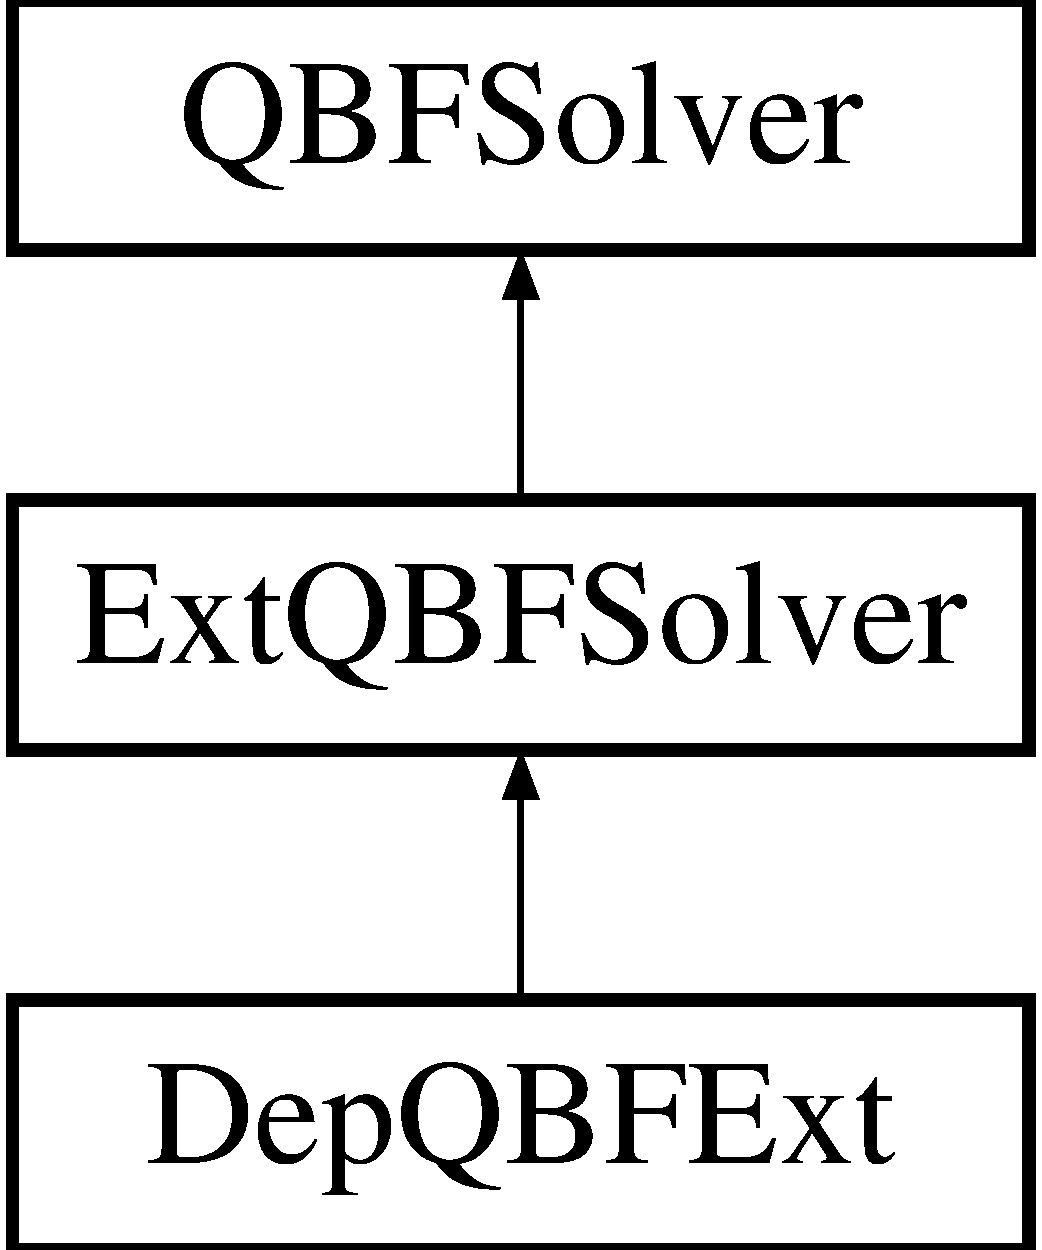
\includegraphics[height=3.000000cm]{classDepQBFExt}
\end{center}
\end{figure}
\subsection*{Public Types}
\begin{DoxyCompactItemize}
\item 
enum \hyperlink{classQBFSolver_ac091e263cb55286cc07b2451bcf4d3c7}{Quant} \{ \hyperlink{classQBFSolver_ac091e263cb55286cc07b2451bcf4d3c7a090ab4a5b262710ccd80e97d72f9a7b3}{E}, 
\hyperlink{classQBFSolver_ac091e263cb55286cc07b2451bcf4d3c7afd6518d5d985aa8346ac071e4c0d8ee0}{A}
 \}
\begin{DoxyCompactList}\small\item\em A type for the different kinds of quantifiers. \end{DoxyCompactList}\end{DoxyCompactItemize}
\subsection*{Public Member Functions}
\begin{DoxyCompactItemize}
\item 
\hyperlink{classDepQBFExt_a21cc5bcaebcf948f6200fcaf198fa9d3}{Dep\-Q\-B\-F\-Ext} (bool use\-\_\-bloqqer=false, size\-\_\-t timeout=0)
\begin{DoxyCompactList}\small\item\em Constructor. \end{DoxyCompactList}\item 
virtual \hyperlink{classDepQBFExt_a6425c670e11fb6f2315171e27f850954}{$\sim$\-Dep\-Q\-B\-F\-Ext} ()
\begin{DoxyCompactList}\small\item\em Destructor. \end{DoxyCompactList}\item 
virtual aiger $\ast$ \hyperlink{classDepQBFExt_a9de37d00363d5ad71eaf03c011314b31}{qbf\-Cert} (const vector$<$ pair$<$ \hyperlink{classVarInfo_a64d1da76cf84fe674e5fef9764ef11cf}{Var\-Info\-::\-Var\-Kind}, \hyperlink{classQBFSolver_ac091e263cb55286cc07b2451bcf4d3c7}{Quant} $>$ $>$ \&quantifier\-\_\-prefix, const \hyperlink{classCNF}{C\-N\-F} \&cnf)
\begin{DoxyCompactList}\small\item\em Executes the Q\-B\-F-\/\-Cert framework to compute Skolem functions for Q\-B\-Fs. \end{DoxyCompactList}\item 
virtual bool \hyperlink{classExtQBFSolver_abec25b97170b79b42b85d1d4ec825a39}{is\-Sat} (const vector$<$ pair$<$ \hyperlink{classVarInfo_a64d1da76cf84fe674e5fef9764ef11cf}{Var\-Info\-::\-Var\-Kind}, \hyperlink{classQBFSolver_ac091e263cb55286cc07b2451bcf4d3c7}{Quant} $>$ $>$ \&quantifier\-\_\-prefix, const \hyperlink{classCNF}{C\-N\-F} \&cnf)
\begin{DoxyCompactList}\small\item\em Checks if a given Q\-B\-F is satisfiable (with quantification over variable kinds). \end{DoxyCompactList}\item 
virtual bool \hyperlink{classExtQBFSolver_adc1bacec3307200dd90b260789e4c808}{is\-Sat} (const vector$<$ pair$<$ vector$<$ int $>$, \hyperlink{classQBFSolver_ac091e263cb55286cc07b2451bcf4d3c7}{Quant} $>$ $>$ \&quantifier\-\_\-prefix, const \hyperlink{classCNF}{C\-N\-F} \&cnf)
\begin{DoxyCompactList}\small\item\em Checks if a given Q\-B\-F is satisfiable (with quantification over variable sets). \end{DoxyCompactList}\item 
virtual bool \hyperlink{classExtQBFSolver_ad66c53343ce9c03eea6e4b5e7753f1b3}{is\-Sat\-Model} (const vector$<$ pair$<$ \hyperlink{classVarInfo_a64d1da76cf84fe674e5fef9764ef11cf}{Var\-Info\-::\-Var\-Kind}, \hyperlink{classQBFSolver_ac091e263cb55286cc07b2451bcf4d3c7}{Quant} $>$ $>$ \&quantifier\-\_\-prefix, const \hyperlink{classCNF}{C\-N\-F} \&cnf, vector$<$ int $>$ \&model)
\begin{DoxyCompactList}\small\item\em Checks satisfiability and extracts a model (quantifying over variable kinds). \end{DoxyCompactList}\item 
virtual bool \hyperlink{classExtQBFSolver_a3add00496f016c2e60a188ce9daa1da1}{is\-Sat\-Model} (const vector$<$ pair$<$ vector$<$ int $>$, \hyperlink{classQBFSolver_ac091e263cb55286cc07b2451bcf4d3c7}{Quant} $>$ $>$ \&quantifier\-\_\-prefix, const \hyperlink{classCNF}{C\-N\-F} \&cnf, vector$<$ int $>$ \&model)
\begin{DoxyCompactList}\small\item\em Checks satisfiability and extracts a model (quantifying over variable sets). \end{DoxyCompactList}\end{DoxyCompactItemize}
\subsection*{Static Public Member Functions}
\begin{DoxyCompactItemize}
\item 
static void \hyperlink{classExtQBFSolver_abebb2acbb5afd5b205254246f39f3e33}{dump\-Q\-B\-F} (const vector$<$ pair$<$ \hyperlink{classVarInfo_a64d1da76cf84fe674e5fef9764ef11cf}{Var\-Info\-::\-Var\-Kind}, \hyperlink{classQBFSolver_ac091e263cb55286cc07b2451bcf4d3c7}{Quant} $>$ $>$ \&quantifier\-\_\-prefix, const \hyperlink{classCNF}{C\-N\-F} \&cnf, const string \&filename)
\begin{DoxyCompactList}\small\item\em Dumps a Q\-B\-F (quantification over variable kinds) into a file in Q\-D\-I\-M\-A\-C\-S format. \end{DoxyCompactList}\item 
static void \hyperlink{classExtQBFSolver_a7e329d1fdce2cf65390930b01cf3a32b}{dump\-Q\-B\-F} (const vector$<$ pair$<$ vector$<$ int $>$, \hyperlink{classQBFSolver_ac091e263cb55286cc07b2451bcf4d3c7}{Quant} $>$ $>$ \&quantifier\-\_\-prefix, const \hyperlink{classCNF}{C\-N\-F} \&cnf, const string \&filename)
\begin{DoxyCompactList}\small\item\em Dumps a Q\-B\-F (quantification over variable kinds) into a file in Q\-D\-I\-M\-A\-C\-S format. \end{DoxyCompactList}\end{DoxyCompactItemize}
\subsection*{Protected Member Functions}
\begin{DoxyCompactItemize}
\item 
virtual string \hyperlink{classDepQBFExt_a64f0c17958bd64cfd20a1f2478f68077}{get\-Solver\-Command} () const 
\begin{DoxyCompactList}\small\item\em Returns the command to execute Dep\-Q\-B\-F. \end{DoxyCompactList}\item 
virtual string \hyperlink{classDepQBFExt_a72321fcf85a52333c0f7e83004a3f119}{get\-Solver\-Command\-Model} () const 
\begin{DoxyCompactList}\small\item\em Returns the command to execute Dep\-Q\-B\-F such that it produces models. \end{DoxyCompactList}\item 
virtual bool \hyperlink{classDepQBFExt_a9dd5f30054b19543393c43796ac43016}{parse\-Model} (int ret, const vector$<$ int $>$ \&get, vector$<$ int $>$ \&model) const 
\begin{DoxyCompactList}\small\item\em Parses the answer of the Q\-B\-F solver to get the satisfiability verdict and a model. \end{DoxyCompactList}\item 
virtual bool \hyperlink{classExtQBFSolver_a11ddbf3980824453238071e8a036f804}{parse\-Answer} (int ret) const 
\begin{DoxyCompactList}\small\item\em Parses the answer of the Q\-B\-F solver to get the satisfiability verdict. \end{DoxyCompactList}\item 
virtual void \hyperlink{classExtQBFSolver_a3ee48837c5e937e4d3a5b3c2a6b761d3}{cleanup} ()
\begin{DoxyCompactList}\small\item\em Deletes the temporary files that have been used for communication. \end{DoxyCompactList}\end{DoxyCompactItemize}
\subsection*{Protected Attributes}
\begin{DoxyCompactItemize}
\item 
bool \hyperlink{classDepQBFExt_a1ac4c3f5db8b564898de69b88e1757e0}{use\-\_\-bloqqer\-\_\-}
\begin{DoxyCompactList}\small\item\em True if bloqqer should be used as a preprocessor. False otherwise. \end{DoxyCompactList}\item 
size\-\_\-t \hyperlink{classDepQBFExt_ac167b3fa37c76fbfabfa855b329a0dfb}{timeout\-\_\-}
\begin{DoxyCompactList}\small\item\em An optional time-\/out in seconds. If set to 0, then no time-\/out will be set. \end{DoxyCompactList}\item 
string \hyperlink{classDepQBFExt_a4c952a6d69e93efc5cd6c5491f85c5b3}{path\-\_\-to\-\_\-deqqbf\-\_\-}
\begin{DoxyCompactList}\small\item\em The path to the Dep\-Q\-B\-F executable. \end{DoxyCompactList}\item 
string \hyperlink{classDepQBFExt_a76b0152b808bde17a2a1324979f82106}{path\-\_\-to\-\_\-bloqqer\-\_\-}
\begin{DoxyCompactList}\small\item\em The path to the Dep\-Q\-B\-F executable. \end{DoxyCompactList}\item 
string \hyperlink{classDepQBFExt_a05676410e9b70c5e83cb13b708e2f178}{path\-\_\-to\-\_\-qbfcert\-\_\-}
\begin{DoxyCompactList}\small\item\em The path to the Q\-B\-F-\/\-Cert script. \end{DoxyCompactList}\item 
string \hyperlink{classExtQBFSolver_a04d2ff483c22a11344e46d66ae7e76b1}{in\-\_\-file\-\_\-name\-\_\-}
\begin{DoxyCompactList}\small\item\em The name of the Q\-D\-I\-M\-A\-C\-S file containing the Q\-B\-F to be solved. \end{DoxyCompactList}\item 
string \hyperlink{classExtQBFSolver_a0efb35aa9b807dec521ad3406eaf664d}{out\-\_\-file\-\_\-name\-\_\-}
\begin{DoxyCompactList}\small\item\em The name of the file that is produced by the Q\-B\-F-\/solver (containing the model). \end{DoxyCompactList}\end{DoxyCompactItemize}
\subsection*{Private Member Functions}
\begin{DoxyCompactItemize}
\item 
\hyperlink{classDepQBFExt_ae711230c91a8990450466d085a34bcc2}{Dep\-Q\-B\-F\-Ext} (const \hyperlink{classDepQBFExt}{Dep\-Q\-B\-F\-Ext} \&other)
\begin{DoxyCompactList}\small\item\em Copy constructor. \end{DoxyCompactList}\item 
\hyperlink{classDepQBFExt}{Dep\-Q\-B\-F\-Ext} \& \hyperlink{classDepQBFExt_a25779db93932e28f4f7cbddaa8636fdb}{operator=} (const \hyperlink{classDepQBFExt}{Dep\-Q\-B\-F\-Ext} \&other)
\begin{DoxyCompactList}\small\item\em Assignment operator. \end{DoxyCompactList}\end{DoxyCompactItemize}


\subsection{Detailed Description}
Calls the Dep\-Q\-B\-F Q\-B\-F-\/solver in a separate process, communicating with files. 

This class represents an interface to the Q\-B\-F-\/solver Dep\-Q\-B\-F (see \href{https://github.com/lonsing/depqbf}{\tt https\-://github.\-com/lonsing/depqbf}). For a given Quantified Boolean formula (a \hyperlink{classCNF}{C\-N\-F} with a quantifier prefix), this class is able to determine satisfiability. Furthermore, in case of satisfiability, it can extract satisfying assignments for variables quantified existentially on the outermost level. The Dep\-Q\-B\-F solver is executed in a separate process. Communication with this process works via files.

Most of work is actually implemented in the base class \hyperlink{classExtQBFSolver}{Ext\-Q\-B\-F\-Solver}. This class mainly overrides some methods which are specific for Dep\-Q\-B\-F. However, it also interfaces the Q\-B\-F-\/\-Cert framework (see \href{http://fmv.jku.at/qbfcert/}{\tt http\-://fmv.\-jku.\-at/qbfcert/}), which uses Dep\-Q\-B\-F to extract Skolem functions for Q\-B\-Fs.

\begin{DoxyAuthor}{Author}
Robert Koenighofer (\href{mailto:robert.koenighofer@iaik.tugraz.at}{\tt robert.\-koenighofer@iaik.\-tugraz.\-at}) 
\end{DoxyAuthor}
\begin{DoxyVersion}{Version}
1.\-2.\-0 
\end{DoxyVersion}


Definition at line 57 of file Dep\-Q\-B\-F\-Ext.\-h.



\subsection{Member Enumeration Documentation}
\hypertarget{classQBFSolver_ac091e263cb55286cc07b2451bcf4d3c7}{\index{Dep\-Q\-B\-F\-Ext@{Dep\-Q\-B\-F\-Ext}!Quant@{Quant}}
\index{Quant@{Quant}!DepQBFExt@{Dep\-Q\-B\-F\-Ext}}
\subsubsection[{Quant}]{\setlength{\rightskip}{0pt plus 5cm}enum {\bf Q\-B\-F\-Solver\-::\-Quant}\hspace{0.3cm}{\ttfamily [inherited]}}}\label{classQBFSolver_ac091e263cb55286cc07b2451bcf4d3c7}


A type for the different kinds of quantifiers. 

\begin{Desc}
\item[Enumerator]\par
\begin{description}
\index{E@{E}!Dep\-Q\-B\-F\-Ext@{Dep\-Q\-B\-F\-Ext}}\index{Dep\-Q\-B\-F\-Ext@{Dep\-Q\-B\-F\-Ext}!E@{E}}\item[{\em 
\hypertarget{classQBFSolver_ac091e263cb55286cc07b2451bcf4d3c7a090ab4a5b262710ccd80e97d72f9a7b3}{E}\label{classQBFSolver_ac091e263cb55286cc07b2451bcf4d3c7a090ab4a5b262710ccd80e97d72f9a7b3}
}]The value for existential quantification. \index{A@{A}!Dep\-Q\-B\-F\-Ext@{Dep\-Q\-B\-F\-Ext}}\index{Dep\-Q\-B\-F\-Ext@{Dep\-Q\-B\-F\-Ext}!A@{A}}\item[{\em 
\hypertarget{classQBFSolver_ac091e263cb55286cc07b2451bcf4d3c7afd6518d5d985aa8346ac071e4c0d8ee0}{A}\label{classQBFSolver_ac091e263cb55286cc07b2451bcf4d3c7afd6518d5d985aa8346ac071e4c0d8ee0}
}]The value for universal quantification. \end{description}
\end{Desc}


Definition at line 56 of file Q\-B\-F\-Solver.\-h.



\subsection{Constructor \& Destructor Documentation}
\hypertarget{classDepQBFExt_a21cc5bcaebcf948f6200fcaf198fa9d3}{\index{Dep\-Q\-B\-F\-Ext@{Dep\-Q\-B\-F\-Ext}!Dep\-Q\-B\-F\-Ext@{Dep\-Q\-B\-F\-Ext}}
\index{Dep\-Q\-B\-F\-Ext@{Dep\-Q\-B\-F\-Ext}!DepQBFExt@{Dep\-Q\-B\-F\-Ext}}
\subsubsection[{Dep\-Q\-B\-F\-Ext}]{\setlength{\rightskip}{0pt plus 5cm}Dep\-Q\-B\-F\-Ext\-::\-Dep\-Q\-B\-F\-Ext (
\begin{DoxyParamCaption}
\item[{bool}]{use\-\_\-bloqqer = {\ttfamily false}, }
\item[{size\-\_\-t}]{timeout = {\ttfamily 0}}
\end{DoxyParamCaption}
)}}\label{classDepQBFExt_a21cc5bcaebcf948f6200fcaf198fa9d3}


Constructor. 


\begin{DoxyParams}{Parameters}
{\em use\-\_\-bloqqer} & True if bloqqer should be used as a preprocessor. False otherwise. \\
\hline
{\em timeout} & An optional time-\/out in seconds. If set to 0, then no time-\/out will be set. At the moment, a time-\/out can only be used with bloqqer. Setting a time-\/out but not using bloqqer, the time-\/out will be ignored. \\
\hline
\end{DoxyParams}


Definition at line 43 of file Dep\-Q\-B\-F\-Ext.\-cpp.



References Options\-::get\-T\-P\-Dir\-Name(), Options\-::instance(), M\-A\-S\-S\-E\-R\-T, path\-\_\-to\-\_\-bloqqer\-\_\-, path\-\_\-to\-\_\-deqqbf\-\_\-, and path\-\_\-to\-\_\-qbfcert\-\_\-.

\hypertarget{classDepQBFExt_a6425c670e11fb6f2315171e27f850954}{\index{Dep\-Q\-B\-F\-Ext@{Dep\-Q\-B\-F\-Ext}!$\sim$\-Dep\-Q\-B\-F\-Ext@{$\sim$\-Dep\-Q\-B\-F\-Ext}}
\index{$\sim$\-Dep\-Q\-B\-F\-Ext@{$\sim$\-Dep\-Q\-B\-F\-Ext}!DepQBFExt@{Dep\-Q\-B\-F\-Ext}}
\subsubsection[{$\sim$\-Dep\-Q\-B\-F\-Ext}]{\setlength{\rightskip}{0pt plus 5cm}Dep\-Q\-B\-F\-Ext\-::$\sim$\-Dep\-Q\-B\-F\-Ext (
\begin{DoxyParamCaption}
{}
\end{DoxyParamCaption}
)\hspace{0.3cm}{\ttfamily [virtual]}}}\label{classDepQBFExt_a6425c670e11fb6f2315171e27f850954}


Destructor. 



Definition at line 57 of file Dep\-Q\-B\-F\-Ext.\-cpp.

\hypertarget{classDepQBFExt_ae711230c91a8990450466d085a34bcc2}{\index{Dep\-Q\-B\-F\-Ext@{Dep\-Q\-B\-F\-Ext}!Dep\-Q\-B\-F\-Ext@{Dep\-Q\-B\-F\-Ext}}
\index{Dep\-Q\-B\-F\-Ext@{Dep\-Q\-B\-F\-Ext}!DepQBFExt@{Dep\-Q\-B\-F\-Ext}}
\subsubsection[{Dep\-Q\-B\-F\-Ext}]{\setlength{\rightskip}{0pt plus 5cm}Dep\-Q\-B\-F\-Ext\-::\-Dep\-Q\-B\-F\-Ext (
\begin{DoxyParamCaption}
\item[{const {\bf Dep\-Q\-B\-F\-Ext} \&}]{other}
\end{DoxyParamCaption}
)\hspace{0.3cm}{\ttfamily [private]}}}\label{classDepQBFExt_ae711230c91a8990450466d085a34bcc2}


Copy constructor. 

The copy constructor is disabled (set private) and not implemented.


\begin{DoxyParams}{Parameters}
{\em other} & The source for creating the copy. \\
\hline
\end{DoxyParams}


\subsection{Member Function Documentation}
\hypertarget{classExtQBFSolver_a3ee48837c5e937e4d3a5b3c2a6b761d3}{\index{Dep\-Q\-B\-F\-Ext@{Dep\-Q\-B\-F\-Ext}!cleanup@{cleanup}}
\index{cleanup@{cleanup}!DepQBFExt@{Dep\-Q\-B\-F\-Ext}}
\subsubsection[{cleanup}]{\setlength{\rightskip}{0pt plus 5cm}void Ext\-Q\-B\-F\-Solver\-::cleanup (
\begin{DoxyParamCaption}
{}
\end{DoxyParamCaption}
)\hspace{0.3cm}{\ttfamily [protected]}, {\ttfamily [virtual]}, {\ttfamily [inherited]}}}\label{classExtQBFSolver_a3ee48837c5e937e4d3a5b3c2a6b761d3}


Deletes the temporary files that have been used for communication. 



Definition at line 217 of file Ext\-Q\-B\-F\-Solver.\-cpp.



References Ext\-Q\-B\-F\-Solver\-::in\-\_\-file\-\_\-name\-\_\-, and Ext\-Q\-B\-F\-Solver\-::out\-\_\-file\-\_\-name\-\_\-.



Referenced by Ext\-Q\-B\-F\-Solver\-::is\-Sat(), Ext\-Q\-B\-F\-Solver\-::is\-Sat\-Model(), and qbf\-Cert().

\hypertarget{classExtQBFSolver_abebb2acbb5afd5b205254246f39f3e33}{\index{Dep\-Q\-B\-F\-Ext@{Dep\-Q\-B\-F\-Ext}!dump\-Q\-B\-F@{dump\-Q\-B\-F}}
\index{dump\-Q\-B\-F@{dump\-Q\-B\-F}!DepQBFExt@{Dep\-Q\-B\-F\-Ext}}
\subsubsection[{dump\-Q\-B\-F}]{\setlength{\rightskip}{0pt plus 5cm}void Ext\-Q\-B\-F\-Solver\-::dump\-Q\-B\-F (
\begin{DoxyParamCaption}
\item[{const vector$<$ pair$<$ {\bf Var\-Info\-::\-Var\-Kind}, {\bf Quant} $>$ $>$ \&}]{quantifier\-\_\-prefix, }
\item[{const {\bf C\-N\-F} \&}]{cnf, }
\item[{const string \&}]{filename}
\end{DoxyParamCaption}
)\hspace{0.3cm}{\ttfamily [static]}, {\ttfamily [inherited]}}}\label{classExtQBFSolver_abebb2acbb5afd5b205254246f39f3e33}


Dumps a Q\-B\-F (quantification over variable kinds) into a file in Q\-D\-I\-M\-A\-C\-S format. 


\begin{DoxyParams}{Parameters}
{\em quantifier\-\_\-prefix} & The quantifier prefix as a vector of pairs. vector\mbox{[}0\mbox{]} is the leftmost (i.\-e., outermost) quantifier block. The pairs in the quantifier\-\_\-prefix assign an existential or universal quantifier to every kind of variable that occurs in the cnf. \\
\hline
{\em cnf} & A Boolean formula in \hyperlink{classCNF}{C\-N\-F}. \\
\hline
{\em filename} & The name of the file (including path) to write to. \\
\hline
\end{DoxyParams}


Definition at line 105 of file Ext\-Q\-B\-F\-Solver.\-cpp.



References Q\-B\-F\-Solver\-::\-E, Var\-Manager\-::get\-Max\-C\-N\-F\-Var(), C\-N\-F\-::get\-Nr\-Of\-Clauses(), Var\-Manager\-::get\-Vars\-Of\-Type(), Var\-Manager\-::instance(), and C\-N\-F\-::to\-String().



Referenced by Dep\-Q\-B\-F\-Api\-::debug\-Check\-Bloqqer\-Model(), Dep\-Q\-B\-F\-Api\-::debug\-Check\-Bloqqer\-Verdict(), Ext\-Q\-B\-F\-Solver\-::is\-Sat(), Ext\-Q\-B\-F\-Solver\-::is\-Sat\-Model(), and qbf\-Cert().

\hypertarget{classExtQBFSolver_a7e329d1fdce2cf65390930b01cf3a32b}{\index{Dep\-Q\-B\-F\-Ext@{Dep\-Q\-B\-F\-Ext}!dump\-Q\-B\-F@{dump\-Q\-B\-F}}
\index{dump\-Q\-B\-F@{dump\-Q\-B\-F}!DepQBFExt@{Dep\-Q\-B\-F\-Ext}}
\subsubsection[{dump\-Q\-B\-F}]{\setlength{\rightskip}{0pt plus 5cm}void Ext\-Q\-B\-F\-Solver\-::dump\-Q\-B\-F (
\begin{DoxyParamCaption}
\item[{const vector$<$ pair$<$ vector$<$ int $>$, {\bf Quant} $>$ $>$ \&}]{quantifier\-\_\-prefix, }
\item[{const {\bf C\-N\-F} \&}]{cnf, }
\item[{const string \&}]{filename}
\end{DoxyParamCaption}
)\hspace{0.3cm}{\ttfamily [static]}, {\ttfamily [inherited]}}}\label{classExtQBFSolver_a7e329d1fdce2cf65390930b01cf3a32b}


Dumps a Q\-B\-F (quantification over variable kinds) into a file in Q\-D\-I\-M\-A\-C\-S format. 


\begin{DoxyParams}{Parameters}
{\em quantifier\-\_\-prefix} & The quantifier prefix as a vector of pairs. vector\mbox{[}0\mbox{]} is the leftmost (i.\-e., outermost) quantifier block. The pairs in the quantifier\-\_\-prefix assign an existential or universal quantifier to different sets of variables occurring in the cnf. \\
\hline
{\em cnf} & A Boolean formula in \hyperlink{classCNF}{C\-N\-F}. \\
\hline
{\em filename} & The name of the file (including path) to write to. \\
\hline
\end{DoxyParams}


Definition at line 138 of file Ext\-Q\-B\-F\-Solver.\-cpp.



References Q\-B\-F\-Solver\-::\-E, C\-N\-F\-::get\-Nr\-Of\-Clauses(), and C\-N\-F\-::to\-String().

\hypertarget{classDepQBFExt_a64f0c17958bd64cfd20a1f2478f68077}{\index{Dep\-Q\-B\-F\-Ext@{Dep\-Q\-B\-F\-Ext}!get\-Solver\-Command@{get\-Solver\-Command}}
\index{get\-Solver\-Command@{get\-Solver\-Command}!DepQBFExt@{Dep\-Q\-B\-F\-Ext}}
\subsubsection[{get\-Solver\-Command}]{\setlength{\rightskip}{0pt plus 5cm}string Dep\-Q\-B\-F\-Ext\-::get\-Solver\-Command (
\begin{DoxyParamCaption}
{}
\end{DoxyParamCaption}
) const\hspace{0.3cm}{\ttfamily [protected]}, {\ttfamily [virtual]}}}\label{classDepQBFExt_a64f0c17958bd64cfd20a1f2478f68077}


Returns the command to execute Dep\-Q\-B\-F. 

\begin{DoxyReturn}{Returns}
The command to execute Dep\-Q\-B\-F. 
\end{DoxyReturn}


Implements \hyperlink{classExtQBFSolver_aec4c2d830f72283e2fbabf4a3f62a640}{Ext\-Q\-B\-F\-Solver}.



Definition at line 82 of file Dep\-Q\-B\-F\-Ext.\-cpp.



References Ext\-Q\-B\-F\-Solver\-::in\-\_\-file\-\_\-name\-\_\-, Ext\-Q\-B\-F\-Solver\-::out\-\_\-file\-\_\-name\-\_\-, path\-\_\-to\-\_\-bloqqer\-\_\-, path\-\_\-to\-\_\-deqqbf\-\_\-, timeout\-\_\-, and use\-\_\-bloqqer\-\_\-.

\hypertarget{classDepQBFExt_a72321fcf85a52333c0f7e83004a3f119}{\index{Dep\-Q\-B\-F\-Ext@{Dep\-Q\-B\-F\-Ext}!get\-Solver\-Command\-Model@{get\-Solver\-Command\-Model}}
\index{get\-Solver\-Command\-Model@{get\-Solver\-Command\-Model}!DepQBFExt@{Dep\-Q\-B\-F\-Ext}}
\subsubsection[{get\-Solver\-Command\-Model}]{\setlength{\rightskip}{0pt plus 5cm}string Dep\-Q\-B\-F\-Ext\-::get\-Solver\-Command\-Model (
\begin{DoxyParamCaption}
{}
\end{DoxyParamCaption}
) const\hspace{0.3cm}{\ttfamily [protected]}, {\ttfamily [virtual]}}}\label{classDepQBFExt_a72321fcf85a52333c0f7e83004a3f119}


Returns the command to execute Dep\-Q\-B\-F such that it produces models. 

\begin{DoxyReturn}{Returns}
The command to execute Dep\-Q\-B\-F such that it produces models. 
\end{DoxyReturn}


Implements \hyperlink{classExtQBFSolver_ac2bc9e4817cfa1a54195d7d9f1c7d3bd}{Ext\-Q\-B\-F\-Solver}.



Definition at line 94 of file Dep\-Q\-B\-F\-Ext.\-cpp.



References Ext\-Q\-B\-F\-Solver\-::in\-\_\-file\-\_\-name\-\_\-, Ext\-Q\-B\-F\-Solver\-::out\-\_\-file\-\_\-name\-\_\-, path\-\_\-to\-\_\-bloqqer\-\_\-, path\-\_\-to\-\_\-deqqbf\-\_\-, timeout\-\_\-, and use\-\_\-bloqqer\-\_\-.

\hypertarget{classExtQBFSolver_abec25b97170b79b42b85d1d4ec825a39}{\index{Dep\-Q\-B\-F\-Ext@{Dep\-Q\-B\-F\-Ext}!is\-Sat@{is\-Sat}}
\index{is\-Sat@{is\-Sat}!DepQBFExt@{Dep\-Q\-B\-F\-Ext}}
\subsubsection[{is\-Sat}]{\setlength{\rightskip}{0pt plus 5cm}bool Ext\-Q\-B\-F\-Solver\-::is\-Sat (
\begin{DoxyParamCaption}
\item[{const vector$<$ pair$<$ {\bf Var\-Info\-::\-Var\-Kind}, {\bf Quant} $>$ $>$ \&}]{quantifier\-\_\-prefix, }
\item[{const {\bf C\-N\-F} \&}]{cnf}
\end{DoxyParamCaption}
)\hspace{0.3cm}{\ttfamily [virtual]}, {\ttfamily [inherited]}}}\label{classExtQBFSolver_abec25b97170b79b42b85d1d4ec825a39}


Checks if a given Q\-B\-F is satisfiable (with quantification over variable kinds). 

The Q\-B\-F consists of a quantifier prefix and a Boolean formula in \hyperlink{classCNF}{C\-N\-F}. The quantifier prefix assigns an existential or universal quantifier to every kind of variable. The Q\-B\-F is dumped into a file, a Q\-B\-F-\/solver is called, and the exit code is used to infer the satisfiability result.


\begin{DoxyExceptions}{Exceptions}
{\em \hyperlink{classDemiurgeException}{Demiurge\-Exception}} & if the solver crashed or a timeout occurred. \\
\hline
\end{DoxyExceptions}

\begin{DoxyParams}{Parameters}
{\em quantifier\-\_\-prefix} & The quantifier prefix as a vector of pairs. vector\mbox{[}0\mbox{]} is the leftmost (i.\-e., outermost) quantifier block. The pairs in the quantifier\-\_\-prefix assign an existential or universal quantifier to every kind of variable that occurs in the cnf. \\
\hline
{\em cnf} & A Boolean formula in \hyperlink{classCNF}{C\-N\-F}. \\
\hline
\end{DoxyParams}
\begin{DoxyReturn}{Returns}
True if the Q\-B\-F is satisfiable, false otherwise. 
\end{DoxyReturn}


Implements \hyperlink{classQBFSolver_a53ef157391b176dfbd2a77a1e31befc3}{Q\-B\-F\-Solver}.



Definition at line 54 of file Ext\-Q\-B\-F\-Solver.\-cpp.



References Ext\-Q\-B\-F\-Solver\-::cleanup(), Ext\-Q\-B\-F\-Solver\-::dump\-Q\-B\-F(), Ext\-Q\-B\-F\-Solver\-::get\-Solver\-Command(), Ext\-Q\-B\-F\-Solver\-::in\-\_\-file\-\_\-name\-\_\-, and Ext\-Q\-B\-F\-Solver\-::parse\-Answer().



Referenced by Q\-B\-F\-Cert\-Impl\-Extractor\-::run().

\hypertarget{classExtQBFSolver_adc1bacec3307200dd90b260789e4c808}{\index{Dep\-Q\-B\-F\-Ext@{Dep\-Q\-B\-F\-Ext}!is\-Sat@{is\-Sat}}
\index{is\-Sat@{is\-Sat}!DepQBFExt@{Dep\-Q\-B\-F\-Ext}}
\subsubsection[{is\-Sat}]{\setlength{\rightskip}{0pt plus 5cm}bool Ext\-Q\-B\-F\-Solver\-::is\-Sat (
\begin{DoxyParamCaption}
\item[{const vector$<$ pair$<$ vector$<$ int $>$, {\bf Quant} $>$ $>$ \&}]{quantifier\-\_\-prefix, }
\item[{const {\bf C\-N\-F} \&}]{cnf}
\end{DoxyParamCaption}
)\hspace{0.3cm}{\ttfamily [virtual]}, {\ttfamily [inherited]}}}\label{classExtQBFSolver_adc1bacec3307200dd90b260789e4c808}


Checks if a given Q\-B\-F is satisfiable (with quantification over variable sets). 

The Q\-B\-F consists of a quantifier prefix and a Boolean formula in \hyperlink{classCNF}{C\-N\-F}. The quantifier prefix assigns an existential or universal quantifier to different sets variable. The Q\-B\-F is dumped into a file, a Q\-B\-F-\/solver is called, and the exit code is used to infer the satisfiability result.


\begin{DoxyExceptions}{Exceptions}
{\em \hyperlink{classDemiurgeException}{Demiurge\-Exception}} & if the solver crashed or a timeout occurred. \\
\hline
\end{DoxyExceptions}

\begin{DoxyParams}{Parameters}
{\em quantifier\-\_\-prefix} & The quantifier prefix as a vector of pairs. vector\mbox{[}0\mbox{]} is the leftmost (i.\-e., outermost) quantifier block. The pairs in the quantifier\-\_\-prefix assign an existential or universal quantifier to different sets of variables occurring in the cnf. \\
\hline
{\em cnf} & A Boolean formula in \hyperlink{classCNF}{C\-N\-F}. \\
\hline
\end{DoxyParams}
\begin{DoxyReturn}{Returns}
True if the Q\-B\-F is satisfiable, false otherwise. 
\end{DoxyReturn}


Implements \hyperlink{classQBFSolver_aca37de5801e36d4749b80b6c8c2023a9}{Q\-B\-F\-Solver}.



Definition at line 66 of file Ext\-Q\-B\-F\-Solver.\-cpp.



References Ext\-Q\-B\-F\-Solver\-::cleanup(), Ext\-Q\-B\-F\-Solver\-::dump\-Q\-B\-F(), Ext\-Q\-B\-F\-Solver\-::get\-Solver\-Command(), Ext\-Q\-B\-F\-Solver\-::in\-\_\-file\-\_\-name\-\_\-, and Ext\-Q\-B\-F\-Solver\-::parse\-Answer().

\hypertarget{classExtQBFSolver_ad66c53343ce9c03eea6e4b5e7753f1b3}{\index{Dep\-Q\-B\-F\-Ext@{Dep\-Q\-B\-F\-Ext}!is\-Sat\-Model@{is\-Sat\-Model}}
\index{is\-Sat\-Model@{is\-Sat\-Model}!DepQBFExt@{Dep\-Q\-B\-F\-Ext}}
\subsubsection[{is\-Sat\-Model}]{\setlength{\rightskip}{0pt plus 5cm}bool Ext\-Q\-B\-F\-Solver\-::is\-Sat\-Model (
\begin{DoxyParamCaption}
\item[{const vector$<$ pair$<$ {\bf Var\-Info\-::\-Var\-Kind}, {\bf Quant} $>$ $>$ \&}]{quantifier\-\_\-prefix, }
\item[{const {\bf C\-N\-F} \&}]{cnf, }
\item[{vector$<$ int $>$ \&}]{model}
\end{DoxyParamCaption}
)\hspace{0.3cm}{\ttfamily [virtual]}, {\ttfamily [inherited]}}}\label{classExtQBFSolver_ad66c53343ce9c03eea6e4b5e7753f1b3}


Checks satisfiability and extracts a model (quantifying over variable kinds). 

Just like \hyperlink{classExtQBFSolver_abec25b97170b79b42b85d1d4ec825a39}{is\-Sat() }, this method checks a quantified Boolean formula for satisfiability. If the Q\-B\-F is satisfiable, this method also extracts a model (a satisfying assignment) for all variables which are quantified existentially on the outermost level. The model is provided as cube\-: negated variables in the cube are F\-A\-L\-S\-E, unnegated ones are T\-R\-U\-E.


\begin{DoxyExceptions}{Exceptions}
{\em \hyperlink{classDemiurgeException}{Demiurge\-Exception}} & if the solver crashed or a timeout occurred. \\
\hline
\end{DoxyExceptions}

\begin{DoxyParams}{Parameters}
{\em quantifier\-\_\-prefix} & The quantifier prefix as a vector of pairs. vector\mbox{[}0\mbox{]} is the leftmost (i.\-e., outermost) quantifier block. The pairs in the quantifier\-\_\-prefix assign an existential or universal quantifier to every kind of variable that occurs in the cnf. \\
\hline
{\em cnf} & A Boolean formula in \hyperlink{classCNF}{C\-N\-F}. \\
\hline
{\em model} & The resulting model in form of a cube in case of satisfiability. Negated variables in the cube are F\-A\-L\-S\-E, unnegated ones are T\-R\-U\-E. If the formula is unsatisfiable (this method returns false) then this parameter is not modified. \\
\hline
\end{DoxyParams}
\begin{DoxyReturn}{Returns}
True if the Q\-B\-F is satisfiable, false otherwise. 
\end{DoxyReturn}


Implements \hyperlink{classQBFSolver_a76fc0c757a2c039816e3e06547f06d5c}{Q\-B\-F\-Solver}.



Definition at line 78 of file Ext\-Q\-B\-F\-Solver.\-cpp.



References Ext\-Q\-B\-F\-Solver\-::cleanup(), Ext\-Q\-B\-F\-Solver\-::dump\-Q\-B\-F(), Ext\-Q\-B\-F\-Solver\-::get\-Solver\-Command\-Model(), Var\-Manager\-::get\-Vars\-Of\-Type(), Ext\-Q\-B\-F\-Solver\-::in\-\_\-file\-\_\-name\-\_\-, Var\-Manager\-::instance(), and Ext\-Q\-B\-F\-Solver\-::parse\-Model().



Referenced by Templ\-Explorer\-::synt\-Q\-B\-F().

\hypertarget{classExtQBFSolver_a3add00496f016c2e60a188ce9daa1da1}{\index{Dep\-Q\-B\-F\-Ext@{Dep\-Q\-B\-F\-Ext}!is\-Sat\-Model@{is\-Sat\-Model}}
\index{is\-Sat\-Model@{is\-Sat\-Model}!DepQBFExt@{Dep\-Q\-B\-F\-Ext}}
\subsubsection[{is\-Sat\-Model}]{\setlength{\rightskip}{0pt plus 5cm}bool Ext\-Q\-B\-F\-Solver\-::is\-Sat\-Model (
\begin{DoxyParamCaption}
\item[{const vector$<$ pair$<$ vector$<$ int $>$, {\bf Quant} $>$ $>$ \&}]{quantifier\-\_\-prefix, }
\item[{const {\bf C\-N\-F} \&}]{cnf, }
\item[{vector$<$ int $>$ \&}]{model}
\end{DoxyParamCaption}
)\hspace{0.3cm}{\ttfamily [virtual]}, {\ttfamily [inherited]}}}\label{classExtQBFSolver_a3add00496f016c2e60a188ce9daa1da1}


Checks satisfiability and extracts a model (quantifying over variable sets). 

Just like \hyperlink{classExtQBFSolver_abec25b97170b79b42b85d1d4ec825a39}{is\-Sat() }, this method checks a quantified Boolean formula for satisfiability. If the Q\-B\-F is satisfiable, this method also extracts a model (a satisfying assignment) for all variables which are quantified existentially on the outermost level. The model is provided as cube\-: negated variables in the cube are F\-A\-L\-S\-E, unnegated ones are T\-R\-U\-E.


\begin{DoxyExceptions}{Exceptions}
{\em \hyperlink{classDemiurgeException}{Demiurge\-Exception}} & if the solver crashed or a timeout occurred. \\
\hline
\end{DoxyExceptions}

\begin{DoxyParams}{Parameters}
{\em quantifier\-\_\-prefix} & The quantifier prefix as a vector of pairs. vector\mbox{[}0\mbox{]} is the leftmost (i.\-e., outermost) quantifier block. The pairs in the quantifier\-\_\-prefix assign an existential or universal quantifier to different sets of variables occurring in the cnf. \\
\hline
{\em cnf} & A Boolean formula in \hyperlink{classCNF}{C\-N\-F}. \\
\hline
{\em model} & The resulting model in form of a cube in case of satisfiability. Negated variables in the cube are F\-A\-L\-S\-E, unnegated ones are T\-R\-U\-E. If the formula is unsatisfiable (this method returns false) then this parameter is not modified. \\
\hline
\end{DoxyParams}
\begin{DoxyReturn}{Returns}
True if the Q\-B\-F is satisfiable, false otherwise. 
\end{DoxyReturn}


Implements \hyperlink{classQBFSolver_a12f2ce57b778b9efe729d63bf881493d}{Q\-B\-F\-Solver}.



Definition at line 92 of file Ext\-Q\-B\-F\-Solver.\-cpp.



References Ext\-Q\-B\-F\-Solver\-::cleanup(), Ext\-Q\-B\-F\-Solver\-::dump\-Q\-B\-F(), Ext\-Q\-B\-F\-Solver\-::get\-Solver\-Command\-Model(), Ext\-Q\-B\-F\-Solver\-::in\-\_\-file\-\_\-name\-\_\-, and Ext\-Q\-B\-F\-Solver\-::parse\-Model().

\hypertarget{classDepQBFExt_a25779db93932e28f4f7cbddaa8636fdb}{\index{Dep\-Q\-B\-F\-Ext@{Dep\-Q\-B\-F\-Ext}!operator=@{operator=}}
\index{operator=@{operator=}!DepQBFExt@{Dep\-Q\-B\-F\-Ext}}
\subsubsection[{operator=}]{\setlength{\rightskip}{0pt plus 5cm}{\bf Dep\-Q\-B\-F\-Ext}\& Dep\-Q\-B\-F\-Ext\-::operator= (
\begin{DoxyParamCaption}
\item[{const {\bf Dep\-Q\-B\-F\-Ext} \&}]{other}
\end{DoxyParamCaption}
)\hspace{0.3cm}{\ttfamily [private]}}}\label{classDepQBFExt_a25779db93932e28f4f7cbddaa8636fdb}


Assignment operator. 

The assignment operator is disabled (set private) and not implemented.


\begin{DoxyParams}{Parameters}
{\em other} & The source for creating the copy. \\
\hline
\end{DoxyParams}
\begin{DoxyReturn}{Returns}
The result of the assignment, i.\-e, $\ast$this. 
\end{DoxyReturn}
\hypertarget{classExtQBFSolver_a11ddbf3980824453238071e8a036f804}{\index{Dep\-Q\-B\-F\-Ext@{Dep\-Q\-B\-F\-Ext}!parse\-Answer@{parse\-Answer}}
\index{parse\-Answer@{parse\-Answer}!DepQBFExt@{Dep\-Q\-B\-F\-Ext}}
\subsubsection[{parse\-Answer}]{\setlength{\rightskip}{0pt plus 5cm}bool Ext\-Q\-B\-F\-Solver\-::parse\-Answer (
\begin{DoxyParamCaption}
\item[{int}]{ret}
\end{DoxyParamCaption}
) const\hspace{0.3cm}{\ttfamily [protected]}, {\ttfamily [virtual]}, {\ttfamily [inherited]}}}\label{classExtQBFSolver_a11ddbf3980824453238071e8a036f804}


Parses the answer of the Q\-B\-F solver to get the satisfiability verdict. 


\begin{DoxyExceptions}{Exceptions}
{\em \hyperlink{classDemiurgeException}{Demiurge\-Exception}} & if the solver crashed or a timeout occurred. \\
\hline
\end{DoxyExceptions}

\begin{DoxyParams}{Parameters}
{\em ret} & The exit code of the process running the Q\-B\-F solver. \\
\hline
\end{DoxyParams}
\begin{DoxyReturn}{Returns}
True in case of satisfiability, false for unsatisfiability. 
\end{DoxyReturn}


Definition at line 180 of file Ext\-Q\-B\-F\-Solver.\-cpp.



Referenced by Ext\-Q\-B\-F\-Solver\-::is\-Sat().

\hypertarget{classDepQBFExt_a9dd5f30054b19543393c43796ac43016}{\index{Dep\-Q\-B\-F\-Ext@{Dep\-Q\-B\-F\-Ext}!parse\-Model@{parse\-Model}}
\index{parse\-Model@{parse\-Model}!DepQBFExt@{Dep\-Q\-B\-F\-Ext}}
\subsubsection[{parse\-Model}]{\setlength{\rightskip}{0pt plus 5cm}bool Dep\-Q\-B\-F\-Ext\-::parse\-Model (
\begin{DoxyParamCaption}
\item[{int}]{ret, }
\item[{const vector$<$ int $>$ \&}]{get, }
\item[{vector$<$ int $>$ \&}]{model}
\end{DoxyParamCaption}
) const\hspace{0.3cm}{\ttfamily [protected]}, {\ttfamily [virtual]}}}\label{classDepQBFExt_a9dd5f30054b19543393c43796ac43016}


Parses the answer of the Q\-B\-F solver to get the satisfiability verdict and a model. 


\begin{DoxyExceptions}{Exceptions}
{\em \hyperlink{classDemiurgeException}{Demiurge\-Exception}} & if the solver crashed or a timeout occurred. \\
\hline
\end{DoxyExceptions}

\begin{DoxyParams}{Parameters}
{\em ret} & The exit code of the process running the Q\-B\-F solver. \\
\hline
{\em get} & The variables of interest for which we want to have a satisfying assignment. \\
\hline
{\em model} & An empty vector. In case of satisfiability, this method will write a satisfying assignment in form of a cube into this vector. \\
\hline
\end{DoxyParams}
\begin{DoxyReturn}{Returns}
True in case of satisfiability, false for unsatisfiability. 
\end{DoxyReturn}


Reimplemented from \hyperlink{classExtQBFSolver_afe52ff8faa21fbdd850b73e8f8cf9839}{Ext\-Q\-B\-F\-Solver}.



Definition at line 106 of file Dep\-Q\-B\-F\-Ext.\-cpp.



References Utils\-::contains(), M\-A\-S\-S\-E\-R\-T, Ext\-Q\-B\-F\-Solver\-::out\-\_\-file\-\_\-name\-\_\-, File\-Utils\-::read\-File(), String\-Utils\-::split\-Lines(), and use\-\_\-bloqqer\-\_\-.

\hypertarget{classDepQBFExt_a9de37d00363d5ad71eaf03c011314b31}{\index{Dep\-Q\-B\-F\-Ext@{Dep\-Q\-B\-F\-Ext}!qbf\-Cert@{qbf\-Cert}}
\index{qbf\-Cert@{qbf\-Cert}!DepQBFExt@{Dep\-Q\-B\-F\-Ext}}
\subsubsection[{qbf\-Cert}]{\setlength{\rightskip}{0pt plus 5cm}aiger $\ast$ Dep\-Q\-B\-F\-Ext\-::qbf\-Cert (
\begin{DoxyParamCaption}
\item[{const vector$<$ pair$<$ {\bf Var\-Info\-::\-Var\-Kind}, {\bf Quant} $>$ $>$ \&}]{quantifier\-\_\-prefix, }
\item[{const {\bf C\-N\-F} \&}]{cnf}
\end{DoxyParamCaption}
)\hspace{0.3cm}{\ttfamily [virtual]}}}\label{classDepQBFExt_a9de37d00363d5ad71eaf03c011314b31}


Executes the Q\-B\-F-\/\-Cert framework to compute Skolem functions for Q\-B\-Fs. 

The Q\-B\-F consists of a quantifier prefix and a Boolean formula in \hyperlink{classCNF}{C\-N\-F}. The quantifier prefix assigns an existential or universal quantifier to every kind of variable.


\begin{DoxyParams}{Parameters}
{\em quantifier\-\_\-prefix} & The quantifier prefix as a vector of pairs. vector\mbox{[}0\mbox{]} is the leftmost (i.\-e., outermost) quantifier block. The pairs in the quantifier\-\_\-prefix assign an existential or universal quantifier to every kind of variable that occurs in the cnf. \\
\hline
{\em cnf} & A Boolean formula in \hyperlink{classCNF}{C\-N\-F}. \\
\hline
\end{DoxyParams}
\begin{DoxyReturn}{Returns}
The resulting Skolem functions in A\-I\-G\-E\-R format. The returned A\-I\-G\-E\-R structure must be deleted by the caller. 
\end{DoxyReturn}


Definition at line 63 of file Dep\-Q\-B\-F\-Ext.\-cpp.



References Ext\-Q\-B\-F\-Solver\-::cleanup(), Ext\-Q\-B\-F\-Solver\-::dump\-Q\-B\-F(), Ext\-Q\-B\-F\-Solver\-::in\-\_\-file\-\_\-name\-\_\-, M\-A\-S\-S\-E\-R\-T, and path\-\_\-to\-\_\-qbfcert\-\_\-.



Referenced by Q\-B\-F\-Cert\-Impl\-Extractor\-::run().



\subsection{Member Data Documentation}
\hypertarget{classExtQBFSolver_a04d2ff483c22a11344e46d66ae7e76b1}{\index{Dep\-Q\-B\-F\-Ext@{Dep\-Q\-B\-F\-Ext}!in\-\_\-file\-\_\-name\-\_\-@{in\-\_\-file\-\_\-name\-\_\-}}
\index{in\-\_\-file\-\_\-name\-\_\-@{in\-\_\-file\-\_\-name\-\_\-}!DepQBFExt@{Dep\-Q\-B\-F\-Ext}}
\subsubsection[{in\-\_\-file\-\_\-name\-\_\-}]{\setlength{\rightskip}{0pt plus 5cm}string Ext\-Q\-B\-F\-Solver\-::in\-\_\-file\-\_\-name\-\_\-\hspace{0.3cm}{\ttfamily [protected]}, {\ttfamily [inherited]}}}\label{classExtQBFSolver_a04d2ff483c22a11344e46d66ae7e76b1}


The name of the Q\-D\-I\-M\-A\-C\-S file containing the Q\-B\-F to be solved. 



Definition at line 232 of file Ext\-Q\-B\-F\-Solver.\-h.



Referenced by Ext\-Q\-B\-F\-Solver\-::cleanup(), Ext\-Q\-B\-F\-Solver\-::\-Ext\-Q\-B\-F\-Solver(), Rareqs\-Ext\-::get\-Solver\-Command(), Qu\-B\-E\-Ext\-::get\-Solver\-Command(), get\-Solver\-Command(), Rareqs\-Ext\-::get\-Solver\-Command\-Model(), Qu\-B\-E\-Ext\-::get\-Solver\-Command\-Model(), get\-Solver\-Command\-Model(), Ext\-Q\-B\-F\-Solver\-::is\-Sat(), Ext\-Q\-B\-F\-Solver\-::is\-Sat\-Model(), and qbf\-Cert().

\hypertarget{classExtQBFSolver_a0efb35aa9b807dec521ad3406eaf664d}{\index{Dep\-Q\-B\-F\-Ext@{Dep\-Q\-B\-F\-Ext}!out\-\_\-file\-\_\-name\-\_\-@{out\-\_\-file\-\_\-name\-\_\-}}
\index{out\-\_\-file\-\_\-name\-\_\-@{out\-\_\-file\-\_\-name\-\_\-}!DepQBFExt@{Dep\-Q\-B\-F\-Ext}}
\subsubsection[{out\-\_\-file\-\_\-name\-\_\-}]{\setlength{\rightskip}{0pt plus 5cm}string Ext\-Q\-B\-F\-Solver\-::out\-\_\-file\-\_\-name\-\_\-\hspace{0.3cm}{\ttfamily [protected]}, {\ttfamily [inherited]}}}\label{classExtQBFSolver_a0efb35aa9b807dec521ad3406eaf664d}


The name of the file that is produced by the Q\-B\-F-\/solver (containing the model). 



Definition at line 237 of file Ext\-Q\-B\-F\-Solver.\-h.



Referenced by Ext\-Q\-B\-F\-Solver\-::cleanup(), Ext\-Q\-B\-F\-Solver\-::\-Ext\-Q\-B\-F\-Solver(), Rareqs\-Ext\-::get\-Solver\-Command(), Qu\-B\-E\-Ext\-::get\-Solver\-Command(), get\-Solver\-Command(), Rareqs\-Ext\-::get\-Solver\-Command\-Model(), Qu\-B\-E\-Ext\-::get\-Solver\-Command\-Model(), get\-Solver\-Command\-Model(), Rareqs\-Ext\-::parse\-Model(), parse\-Model(), and Ext\-Q\-B\-F\-Solver\-::parse\-Model().

\hypertarget{classDepQBFExt_a76b0152b808bde17a2a1324979f82106}{\index{Dep\-Q\-B\-F\-Ext@{Dep\-Q\-B\-F\-Ext}!path\-\_\-to\-\_\-bloqqer\-\_\-@{path\-\_\-to\-\_\-bloqqer\-\_\-}}
\index{path\-\_\-to\-\_\-bloqqer\-\_\-@{path\-\_\-to\-\_\-bloqqer\-\_\-}!DepQBFExt@{Dep\-Q\-B\-F\-Ext}}
\subsubsection[{path\-\_\-to\-\_\-bloqqer\-\_\-}]{\setlength{\rightskip}{0pt plus 5cm}string Dep\-Q\-B\-F\-Ext\-::path\-\_\-to\-\_\-bloqqer\-\_\-\hspace{0.3cm}{\ttfamily [protected]}}}\label{classDepQBFExt_a76b0152b808bde17a2a1324979f82106}


The path to the Dep\-Q\-B\-F executable. 



Definition at line 139 of file Dep\-Q\-B\-F\-Ext.\-h.



Referenced by Dep\-Q\-B\-F\-Ext(), get\-Solver\-Command(), and get\-Solver\-Command\-Model().

\hypertarget{classDepQBFExt_a4c952a6d69e93efc5cd6c5491f85c5b3}{\index{Dep\-Q\-B\-F\-Ext@{Dep\-Q\-B\-F\-Ext}!path\-\_\-to\-\_\-deqqbf\-\_\-@{path\-\_\-to\-\_\-deqqbf\-\_\-}}
\index{path\-\_\-to\-\_\-deqqbf\-\_\-@{path\-\_\-to\-\_\-deqqbf\-\_\-}!DepQBFExt@{Dep\-Q\-B\-F\-Ext}}
\subsubsection[{path\-\_\-to\-\_\-deqqbf\-\_\-}]{\setlength{\rightskip}{0pt plus 5cm}string Dep\-Q\-B\-F\-Ext\-::path\-\_\-to\-\_\-deqqbf\-\_\-\hspace{0.3cm}{\ttfamily [protected]}}}\label{classDepQBFExt_a4c952a6d69e93efc5cd6c5491f85c5b3}


The path to the Dep\-Q\-B\-F executable. 



Definition at line 134 of file Dep\-Q\-B\-F\-Ext.\-h.



Referenced by Dep\-Q\-B\-F\-Ext(), get\-Solver\-Command(), and get\-Solver\-Command\-Model().

\hypertarget{classDepQBFExt_a05676410e9b70c5e83cb13b708e2f178}{\index{Dep\-Q\-B\-F\-Ext@{Dep\-Q\-B\-F\-Ext}!path\-\_\-to\-\_\-qbfcert\-\_\-@{path\-\_\-to\-\_\-qbfcert\-\_\-}}
\index{path\-\_\-to\-\_\-qbfcert\-\_\-@{path\-\_\-to\-\_\-qbfcert\-\_\-}!DepQBFExt@{Dep\-Q\-B\-F\-Ext}}
\subsubsection[{path\-\_\-to\-\_\-qbfcert\-\_\-}]{\setlength{\rightskip}{0pt plus 5cm}string Dep\-Q\-B\-F\-Ext\-::path\-\_\-to\-\_\-qbfcert\-\_\-\hspace{0.3cm}{\ttfamily [protected]}}}\label{classDepQBFExt_a05676410e9b70c5e83cb13b708e2f178}


The path to the Q\-B\-F-\/\-Cert script. 



Definition at line 144 of file Dep\-Q\-B\-F\-Ext.\-h.



Referenced by Dep\-Q\-B\-F\-Ext(), and qbf\-Cert().

\hypertarget{classDepQBFExt_ac167b3fa37c76fbfabfa855b329a0dfb}{\index{Dep\-Q\-B\-F\-Ext@{Dep\-Q\-B\-F\-Ext}!timeout\-\_\-@{timeout\-\_\-}}
\index{timeout\-\_\-@{timeout\-\_\-}!DepQBFExt@{Dep\-Q\-B\-F\-Ext}}
\subsubsection[{timeout\-\_\-}]{\setlength{\rightskip}{0pt plus 5cm}size\-\_\-t Dep\-Q\-B\-F\-Ext\-::timeout\-\_\-\hspace{0.3cm}{\ttfamily [protected]}}}\label{classDepQBFExt_ac167b3fa37c76fbfabfa855b329a0dfb}


An optional time-\/out in seconds. If set to 0, then no time-\/out will be set. 



Definition at line 129 of file Dep\-Q\-B\-F\-Ext.\-h.



Referenced by get\-Solver\-Command(), and get\-Solver\-Command\-Model().

\hypertarget{classDepQBFExt_a1ac4c3f5db8b564898de69b88e1757e0}{\index{Dep\-Q\-B\-F\-Ext@{Dep\-Q\-B\-F\-Ext}!use\-\_\-bloqqer\-\_\-@{use\-\_\-bloqqer\-\_\-}}
\index{use\-\_\-bloqqer\-\_\-@{use\-\_\-bloqqer\-\_\-}!DepQBFExt@{Dep\-Q\-B\-F\-Ext}}
\subsubsection[{use\-\_\-bloqqer\-\_\-}]{\setlength{\rightskip}{0pt plus 5cm}bool Dep\-Q\-B\-F\-Ext\-::use\-\_\-bloqqer\-\_\-\hspace{0.3cm}{\ttfamily [protected]}}}\label{classDepQBFExt_a1ac4c3f5db8b564898de69b88e1757e0}


True if bloqqer should be used as a preprocessor. False otherwise. 



Definition at line 124 of file Dep\-Q\-B\-F\-Ext.\-h.



Referenced by get\-Solver\-Command(), get\-Solver\-Command\-Model(), and parse\-Model().



The documentation for this class was generated from the following files\-:\begin{DoxyCompactItemize}
\item 
src/\hyperlink{DepQBFExt_8h}{Dep\-Q\-B\-F\-Ext.\-h}\item 
src/\hyperlink{DepQBFExt_8cpp}{Dep\-Q\-B\-F\-Ext.\-cpp}\end{DoxyCompactItemize}

\hypertarget{classEPRSynthesizer}{\section{E\-P\-R\-Synthesizer Class Reference}
\label{classEPRSynthesizer}\index{E\-P\-R\-Synthesizer@{E\-P\-R\-Synthesizer}}
}


Implements a synthesis method based on reduction to E\-P\-R.  




{\ttfamily \#include $<$E\-P\-R\-Synthesizer.\-h$>$}

Inheritance diagram for E\-P\-R\-Synthesizer\-:\begin{figure}[H]
\begin{center}
\leavevmode
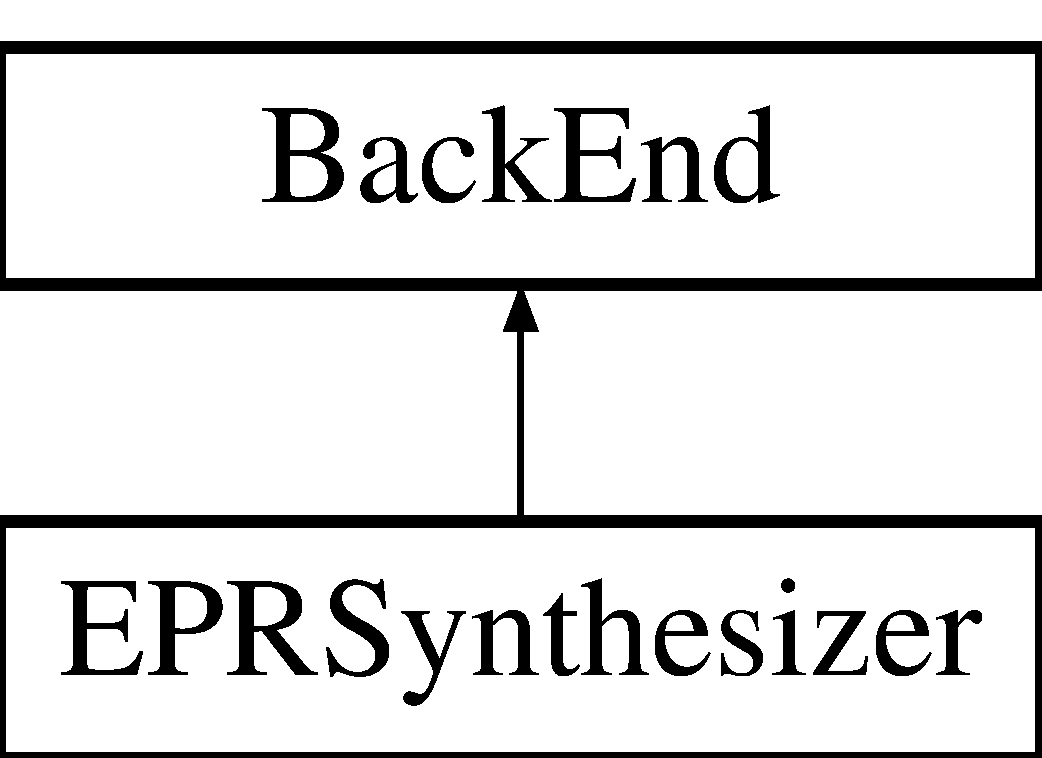
\includegraphics[height=2.000000cm]{classEPRSynthesizer}
\end{center}
\end{figure}
\subsection*{Public Member Functions}
\begin{DoxyCompactItemize}
\item 
\hyperlink{classEPRSynthesizer_a9798c774af30ce7f82564386f6f32d33}{E\-P\-R\-Synthesizer} ()
\begin{DoxyCompactList}\small\item\em Constructor. \end{DoxyCompactList}\item 
virtual \hyperlink{classEPRSynthesizer_a0299d7f7b8dcc26c13ab0b6268e9f974}{$\sim$\-E\-P\-R\-Synthesizer} ()
\begin{DoxyCompactList}\small\item\em Destructor. \end{DoxyCompactList}\item 
virtual bool \hyperlink{classEPRSynthesizer_ab5eb613a7e5e4f8d408938531f745e4e}{run} ()
\begin{DoxyCompactList}\small\item\em Executes the back-\/end (constructs an E\-P\-R formula an passes it to i\-Prover). \end{DoxyCompactList}\end{DoxyCompactItemize}
\subsection*{Protected Member Functions}
\begin{DoxyCompactItemize}
\item 
void \hyperlink{classEPRSynthesizer_ab2815225b4bf61a52b8104b19aae6bcf}{add\-Clause} (const string \&clause, string comment=\char`\"{}\char`\"{})
\begin{DoxyCompactList}\small\item\em A helper that adds a clause to the E\-P\-R formula in T\-P\-T\-P format. \end{DoxyCompactList}\item 
unsigned \hyperlink{classEPRSynthesizer_afd429d29479abe7c3f78a232750a0e53}{neg} (unsigned aig\-\_\-lit)
\begin{DoxyCompactList}\small\item\em A helper to negate an A\-I\-G\-E\-R literal. \end{DoxyCompactList}\end{DoxyCompactItemize}
\subsection*{Protected Attributes}
\begin{DoxyCompactItemize}
\item 
ostringstream \hyperlink{classEPRSynthesizer_a5b9074e1ca3d1a12150c6ae639f475fa}{tptp\-\_\-query\-\_\-}
\begin{DoxyCompactList}\small\item\em The E\-P\-R formula in T\-P\-T\-P format. \end{DoxyCompactList}\item 
size\-\_\-t \hyperlink{classEPRSynthesizer_a14d30bb922f975a1f195965d876784cb}{next\-\_\-clause\-\_\-nr\-\_\-}
\begin{DoxyCompactList}\small\item\em A monotonic counter to assign unique I\-Ds to clauses. \end{DoxyCompactList}\item 
string \hyperlink{classEPRSynthesizer_ac7fc7beb51f9c27e42941e8e20882540}{path\-\_\-to\-\_\-iprover\-\_\-}
\begin{DoxyCompactList}\small\item\em The path to the i\-Prover executable. \end{DoxyCompactList}\item 
string \hyperlink{classEPRSynthesizer_a95c4d232fec2376be891c6ddc96610ce}{in\-\_\-file\-\_\-name\-\_\-}
\begin{DoxyCompactList}\small\item\em The name of the input file (containing the E\-P\-R formula) that is solved by i\-Prover. \end{DoxyCompactList}\item 
string \hyperlink{classEPRSynthesizer_a40ca45e5284a5c24964730beb17d76b8}{out\-\_\-file\-\_\-name\-\_\-}
\begin{DoxyCompactList}\small\item\em The name of the file containing the response from i\-Prover. \end{DoxyCompactList}\end{DoxyCompactItemize}
\subsection*{Private Member Functions}
\begin{DoxyCompactItemize}
\item 
\hyperlink{classEPRSynthesizer_a50010185f31a7d17a2082d2fe81a0aa9}{E\-P\-R\-Synthesizer} (const \hyperlink{classEPRSynthesizer}{E\-P\-R\-Synthesizer} \&other)
\begin{DoxyCompactList}\small\item\em Copy constructor. \end{DoxyCompactList}\item 
\hyperlink{classEPRSynthesizer}{E\-P\-R\-Synthesizer} \& \hyperlink{classEPRSynthesizer_a3edccf1e4b274eb7ac1f2bbefa2e4d0b}{operator=} (const \hyperlink{classEPRSynthesizer}{E\-P\-R\-Synthesizer} \&other)
\begin{DoxyCompactList}\small\item\em Assignment operator. \end{DoxyCompactList}\end{DoxyCompactItemize}


\subsection{Detailed Description}
Implements a synthesis method based on reduction to E\-P\-R. 

E\-P\-R (Effectively Propositional Logic) is a subset of first-\/order logic. E\-P\-R formulas are of the form exists A\-: forall B\-: F, where A and B are sets of domain variables, and F is a function-\/free formula in \hyperlink{classCNF}{C\-N\-F}. F can contain predicates over the variables of A and B. These predicates are implicitly existentially quantified.

This class creates the following E\-P\-R formula\-: forall x,i,x'\-: (I(x) =$>$ W(x)) A\-N\-D (W(x) =$>$ P(x)) A\-N\-D (W(x) A\-N\-D T(x,i,C(x,i),x') =$>$ W(x')) Here, x,i, and x' are actually domain variables (and not Boolean variables), but there is a one-\/to-\/one mapping. W is a fresh predicate over the state variables. It represents the winning region. C(x,i) is a set of predicates, one for each control signal. These predicates represent the implementation of the control signals. The challenging part in constructing this E\-P\-R formula is actually an efficient encoding of the transition relation T in E\-P\-R. In the A\-I\-G\-E\-R representation (and also in the \hyperlink{classCNF}{C\-N\-F} representation) the transition relation T uses many temporary variables. The problem is that they are all quantified existentially, which means that they have to be skolemized with predicates to get a valid E\-P\-R formula. We analyze the structure of the A\-I\-G\-E\-R graph in order to find out the minimal dependencies for all these predicates. This is supposed to increase the performance. Then the class uses i\-Prover (\href{http://www.cs.man.ac.uk/~korovink/iprover/}{\tt http\-://www.\-cs.\-man.\-ac.\-uk/$\sim$korovink/iprover/}) to solve the formula. i\-Prover cannot only give a Y\-E\-S/\-No answer for the satisfiability question. It can also construct functions for the predicates. That is, i\-Prover gives us the winning region together with implementations for all control signals. It solves the synthesis problem completely (and does not only compute a winning region).

\begin{DoxyRefDesc}{Todo}
\item[\hyperlink{todo__todo000001}{Todo}]\-: At the moment we only construct the formula, and parse back the answer to the realizability question. Parsing back the implementation for the controllable signals remains to be done. (The i\-Prover page promises to release a new version with more output formats soon.) \end{DoxyRefDesc}
\begin{DoxyAuthor}{Author}
Robert Koenighofer (\href{mailto:robert.koenighofer@iaik.tugraz.at}{\tt robert.\-koenighofer@iaik.\-tugraz.\-at}) 
\end{DoxyAuthor}
\begin{DoxyVersion}{Version}
1.\-1.\-0 
\end{DoxyVersion}


Definition at line 73 of file E\-P\-R\-Synthesizer.\-h.



\subsection{Constructor \& Destructor Documentation}
\hypertarget{classEPRSynthesizer_a9798c774af30ce7f82564386f6f32d33}{\index{E\-P\-R\-Synthesizer@{E\-P\-R\-Synthesizer}!E\-P\-R\-Synthesizer@{E\-P\-R\-Synthesizer}}
\index{E\-P\-R\-Synthesizer@{E\-P\-R\-Synthesizer}!EPRSynthesizer@{E\-P\-R\-Synthesizer}}
\subsubsection[{E\-P\-R\-Synthesizer}]{\setlength{\rightskip}{0pt plus 5cm}E\-P\-R\-Synthesizer\-::\-E\-P\-R\-Synthesizer (
\begin{DoxyParamCaption}
{}
\end{DoxyParamCaption}
)}}\label{classEPRSynthesizer_a9798c774af30ce7f82564386f6f32d33}


Constructor. 



Definition at line 41 of file E\-P\-R\-Synthesizer.\-cpp.



References Options\-::get\-T\-P\-Dir\-Name(), Options\-::get\-Unique\-Tmp\-File\-Name(), in\-\_\-file\-\_\-name\-\_\-, Options\-::instance(), out\-\_\-file\-\_\-name\-\_\-, and path\-\_\-to\-\_\-iprover\-\_\-.

\hypertarget{classEPRSynthesizer_a0299d7f7b8dcc26c13ab0b6268e9f974}{\index{E\-P\-R\-Synthesizer@{E\-P\-R\-Synthesizer}!$\sim$\-E\-P\-R\-Synthesizer@{$\sim$\-E\-P\-R\-Synthesizer}}
\index{$\sim$\-E\-P\-R\-Synthesizer@{$\sim$\-E\-P\-R\-Synthesizer}!EPRSynthesizer@{E\-P\-R\-Synthesizer}}
\subsubsection[{$\sim$\-E\-P\-R\-Synthesizer}]{\setlength{\rightskip}{0pt plus 5cm}E\-P\-R\-Synthesizer\-::$\sim$\-E\-P\-R\-Synthesizer (
\begin{DoxyParamCaption}
{}
\end{DoxyParamCaption}
)\hspace{0.3cm}{\ttfamily [virtual]}}}\label{classEPRSynthesizer_a0299d7f7b8dcc26c13ab0b6268e9f974}


Destructor. 



Definition at line 49 of file E\-P\-R\-Synthesizer.\-cpp.

\hypertarget{classEPRSynthesizer_a50010185f31a7d17a2082d2fe81a0aa9}{\index{E\-P\-R\-Synthesizer@{E\-P\-R\-Synthesizer}!E\-P\-R\-Synthesizer@{E\-P\-R\-Synthesizer}}
\index{E\-P\-R\-Synthesizer@{E\-P\-R\-Synthesizer}!EPRSynthesizer@{E\-P\-R\-Synthesizer}}
\subsubsection[{E\-P\-R\-Synthesizer}]{\setlength{\rightskip}{0pt plus 5cm}E\-P\-R\-Synthesizer\-::\-E\-P\-R\-Synthesizer (
\begin{DoxyParamCaption}
\item[{const {\bf E\-P\-R\-Synthesizer} \&}]{other}
\end{DoxyParamCaption}
)\hspace{0.3cm}{\ttfamily [private]}}}\label{classEPRSynthesizer_a50010185f31a7d17a2082d2fe81a0aa9}


Copy constructor. 

The copy constructor is disabled (set private) and not implemented.


\begin{DoxyParams}{Parameters}
{\em other} & The source for creating the copy. \\
\hline
\end{DoxyParams}


\subsection{Member Function Documentation}
\hypertarget{classEPRSynthesizer_ab2815225b4bf61a52b8104b19aae6bcf}{\index{E\-P\-R\-Synthesizer@{E\-P\-R\-Synthesizer}!add\-Clause@{add\-Clause}}
\index{add\-Clause@{add\-Clause}!EPRSynthesizer@{E\-P\-R\-Synthesizer}}
\subsubsection[{add\-Clause}]{\setlength{\rightskip}{0pt plus 5cm}void E\-P\-R\-Synthesizer\-::add\-Clause (
\begin{DoxyParamCaption}
\item[{const string \&}]{clause, }
\item[{string}]{comment = {\ttfamily \char`\"{}\char`\"{}}}
\end{DoxyParamCaption}
)\hspace{0.3cm}{\ttfamily [protected]}}}\label{classEPRSynthesizer_ab2815225b4bf61a52b8104b19aae6bcf}


A helper that adds a clause to the E\-P\-R formula in T\-P\-T\-P format. 

The clause is assigned a unique I\-D, and is added to the tptp\-\_\-query\-\_\- in a nicely formatted form, together with an optional comment.


\begin{DoxyParams}{Parameters}
{\em clause} & A string representation of the clause to add. \\
\hline
{\em comment} & A comment (useful for debugging). This parameter is optional. \\
\hline
\end{DoxyParams}


Definition at line 332 of file E\-P\-R\-Synthesizer.\-cpp.



References next\-\_\-clause\-\_\-nr\-\_\-, and tptp\-\_\-query\-\_\-.



Referenced by run().

\hypertarget{classEPRSynthesizer_afd429d29479abe7c3f78a232750a0e53}{\index{E\-P\-R\-Synthesizer@{E\-P\-R\-Synthesizer}!neg@{neg}}
\index{neg@{neg}!EPRSynthesizer@{E\-P\-R\-Synthesizer}}
\subsubsection[{neg}]{\setlength{\rightskip}{0pt plus 5cm}unsigned E\-P\-R\-Synthesizer\-::neg (
\begin{DoxyParamCaption}
\item[{unsigned}]{aig\-\_\-lit}
\end{DoxyParamCaption}
)\hspace{0.3cm}{\ttfamily [protected]}}}\label{classEPRSynthesizer_afd429d29479abe7c3f78a232750a0e53}


A helper to negate an A\-I\-G\-E\-R literal. 


\begin{DoxyParams}{Parameters}
{\em aig\-\_\-lit} & An A\-I\-G\-E\-R literal. \\
\hline
\end{DoxyParams}
\begin{DoxyReturn}{Returns}
The negation of the passed A\-I\-G\-E\-R literal. 
\end{DoxyReturn}


Definition at line 344 of file E\-P\-R\-Synthesizer.\-cpp.



Referenced by run().

\hypertarget{classEPRSynthesizer_a3edccf1e4b274eb7ac1f2bbefa2e4d0b}{\index{E\-P\-R\-Synthesizer@{E\-P\-R\-Synthesizer}!operator=@{operator=}}
\index{operator=@{operator=}!EPRSynthesizer@{E\-P\-R\-Synthesizer}}
\subsubsection[{operator=}]{\setlength{\rightskip}{0pt plus 5cm}{\bf E\-P\-R\-Synthesizer}\& E\-P\-R\-Synthesizer\-::operator= (
\begin{DoxyParamCaption}
\item[{const {\bf E\-P\-R\-Synthesizer} \&}]{other}
\end{DoxyParamCaption}
)\hspace{0.3cm}{\ttfamily [private]}}}\label{classEPRSynthesizer_a3edccf1e4b274eb7ac1f2bbefa2e4d0b}


Assignment operator. 

The assignment operator is disabled (set private) and not implemented.


\begin{DoxyParams}{Parameters}
{\em other} & The source for creating the copy. \\
\hline
\end{DoxyParams}
\begin{DoxyReturn}{Returns}
The result of the assignment, i.\-e, $\ast$this. 
\end{DoxyReturn}
\hypertarget{classEPRSynthesizer_ab5eb613a7e5e4f8d408938531f745e4e}{\index{E\-P\-R\-Synthesizer@{E\-P\-R\-Synthesizer}!run@{run}}
\index{run@{run}!EPRSynthesizer@{E\-P\-R\-Synthesizer}}
\subsubsection[{run}]{\setlength{\rightskip}{0pt plus 5cm}bool E\-P\-R\-Synthesizer\-::run (
\begin{DoxyParamCaption}
{}
\end{DoxyParamCaption}
)\hspace{0.3cm}{\ttfamily [virtual]}}}\label{classEPRSynthesizer_ab5eb613a7e5e4f8d408938531f745e4e}


Executes the back-\/end (constructs an E\-P\-R formula an passes it to i\-Prover). 

This method is the workhorse of this class. It constructs the following E\-P\-R formula in T\-P\-T\-P format\-: forall x,i,x'\-: (I(x) =$>$ W(x)) A\-N\-D (W(x) =$>$ P(x)) A\-N\-D (W(x) A\-N\-D T(x,i,C(x,i),x') =$>$ W(x')) Here, x,i, and x' are actually domain variables (and not Boolean variables), but there is a one-\/to-\/one mapping. W is a fresh predicate over the state variables. It represents the winning region. C(x,i) is a set of predicates, one for each control signal. These predicates represent the implementation of the control signals. The challenging part in constructing this E\-P\-R formula is actually an efficient encoding of the transition relation T in E\-P\-R. In the A\-I\-G\-E\-R representation (and also in the \hyperlink{classCNF}{C\-N\-F} representation) the transition relation T uses many temporary variables. The problem is that they are all quantified existentially, which means that they have to be skolemized with predicates to get a valid E\-P\-R formula. We analyze the structure of the A\-I\-G\-E\-R graph in order to find out the minimal dependencies for all these predicates. This is supposed to increase the performance. After constructing the E\-P\-R formula this method then calls i\-Prover (\href{http://www.cs.man.ac.uk/~korovink/iprover/}{\tt http\-://www.\-cs.\-man.\-ac.\-uk/$\sim$korovink/iprover/}) to solve it. i\-Prover cannot only give a Y\-E\-S/\-No answer for the satisfiability question. It can also construct functions for the predicates. That is, i\-Prover gives us the winning region together with implementations for all control signals. It solves the synthesis problem completely (and does not only compute a winning region).

\begin{DoxyRefDesc}{Todo}
\item[\hyperlink{todo__todo000002}{Todo}]\-: At the moment we only construct the formula, and parse back the answer to the realizability question. Parsing back the implementation for the controllable signals remains to be done. (The i\-Prover page promises to release a new version with more output formats soon.) \end{DoxyRefDesc}
\begin{DoxyReturn}{Returns}
True if the specification was realizable, false otherwise. 
\end{DoxyReturn}


Implements \hyperlink{classBackEnd_a099e717dc71e9cc2d838b1ca86340590}{Back\-End}.



Definition at line 55 of file E\-P\-R\-Synthesizer.\-cpp.



References add\-Clause(), Options\-::get\-Aig\-In\-File\-Name(), in\-\_\-file\-\_\-name\-\_\-, Options\-::instance(), L\-\_\-\-E\-R\-R, L\-\_\-\-R\-E\-S, M\-A\-S\-S\-E\-R\-T, neg(), out\-\_\-file\-\_\-name\-\_\-, path\-\_\-to\-\_\-iprover\-\_\-, File\-Utils\-::read\-File(), String\-Utils\-::to\-Lower\-Case(), tptp\-\_\-query\-\_\-, and File\-Utils\-::write\-File().



\subsection{Member Data Documentation}
\hypertarget{classEPRSynthesizer_a95c4d232fec2376be891c6ddc96610ce}{\index{E\-P\-R\-Synthesizer@{E\-P\-R\-Synthesizer}!in\-\_\-file\-\_\-name\-\_\-@{in\-\_\-file\-\_\-name\-\_\-}}
\index{in\-\_\-file\-\_\-name\-\_\-@{in\-\_\-file\-\_\-name\-\_\-}!EPRSynthesizer@{E\-P\-R\-Synthesizer}}
\subsubsection[{in\-\_\-file\-\_\-name\-\_\-}]{\setlength{\rightskip}{0pt plus 5cm}string E\-P\-R\-Synthesizer\-::in\-\_\-file\-\_\-name\-\_\-\hspace{0.3cm}{\ttfamily [protected]}}}\label{classEPRSynthesizer_a95c4d232fec2376be891c6ddc96610ce}


The name of the input file (containing the E\-P\-R formula) that is solved by i\-Prover. 



Definition at line 160 of file E\-P\-R\-Synthesizer.\-h.



Referenced by E\-P\-R\-Synthesizer(), and run().

\hypertarget{classEPRSynthesizer_a14d30bb922f975a1f195965d876784cb}{\index{E\-P\-R\-Synthesizer@{E\-P\-R\-Synthesizer}!next\-\_\-clause\-\_\-nr\-\_\-@{next\-\_\-clause\-\_\-nr\-\_\-}}
\index{next\-\_\-clause\-\_\-nr\-\_\-@{next\-\_\-clause\-\_\-nr\-\_\-}!EPRSynthesizer@{E\-P\-R\-Synthesizer}}
\subsubsection[{next\-\_\-clause\-\_\-nr\-\_\-}]{\setlength{\rightskip}{0pt plus 5cm}size\-\_\-t E\-P\-R\-Synthesizer\-::next\-\_\-clause\-\_\-nr\-\_\-\hspace{0.3cm}{\ttfamily [protected]}}}\label{classEPRSynthesizer_a14d30bb922f975a1f195965d876784cb}


A monotonic counter to assign unique I\-Ds to clauses. 



Definition at line 150 of file E\-P\-R\-Synthesizer.\-h.



Referenced by add\-Clause().

\hypertarget{classEPRSynthesizer_a40ca45e5284a5c24964730beb17d76b8}{\index{E\-P\-R\-Synthesizer@{E\-P\-R\-Synthesizer}!out\-\_\-file\-\_\-name\-\_\-@{out\-\_\-file\-\_\-name\-\_\-}}
\index{out\-\_\-file\-\_\-name\-\_\-@{out\-\_\-file\-\_\-name\-\_\-}!EPRSynthesizer@{E\-P\-R\-Synthesizer}}
\subsubsection[{out\-\_\-file\-\_\-name\-\_\-}]{\setlength{\rightskip}{0pt plus 5cm}string E\-P\-R\-Synthesizer\-::out\-\_\-file\-\_\-name\-\_\-\hspace{0.3cm}{\ttfamily [protected]}}}\label{classEPRSynthesizer_a40ca45e5284a5c24964730beb17d76b8}


The name of the file containing the response from i\-Prover. 



Definition at line 165 of file E\-P\-R\-Synthesizer.\-h.



Referenced by E\-P\-R\-Synthesizer(), and run().

\hypertarget{classEPRSynthesizer_ac7fc7beb51f9c27e42941e8e20882540}{\index{E\-P\-R\-Synthesizer@{E\-P\-R\-Synthesizer}!path\-\_\-to\-\_\-iprover\-\_\-@{path\-\_\-to\-\_\-iprover\-\_\-}}
\index{path\-\_\-to\-\_\-iprover\-\_\-@{path\-\_\-to\-\_\-iprover\-\_\-}!EPRSynthesizer@{E\-P\-R\-Synthesizer}}
\subsubsection[{path\-\_\-to\-\_\-iprover\-\_\-}]{\setlength{\rightskip}{0pt plus 5cm}string E\-P\-R\-Synthesizer\-::path\-\_\-to\-\_\-iprover\-\_\-\hspace{0.3cm}{\ttfamily [protected]}}}\label{classEPRSynthesizer_ac7fc7beb51f9c27e42941e8e20882540}


The path to the i\-Prover executable. 



Definition at line 155 of file E\-P\-R\-Synthesizer.\-h.



Referenced by E\-P\-R\-Synthesizer(), and run().

\hypertarget{classEPRSynthesizer_a5b9074e1ca3d1a12150c6ae639f475fa}{\index{E\-P\-R\-Synthesizer@{E\-P\-R\-Synthesizer}!tptp\-\_\-query\-\_\-@{tptp\-\_\-query\-\_\-}}
\index{tptp\-\_\-query\-\_\-@{tptp\-\_\-query\-\_\-}!EPRSynthesizer@{E\-P\-R\-Synthesizer}}
\subsubsection[{tptp\-\_\-query\-\_\-}]{\setlength{\rightskip}{0pt plus 5cm}ostringstream E\-P\-R\-Synthesizer\-::tptp\-\_\-query\-\_\-\hspace{0.3cm}{\ttfamily [protected]}}}\label{classEPRSynthesizer_a5b9074e1ca3d1a12150c6ae639f475fa}


The E\-P\-R formula in T\-P\-T\-P format. 



Definition at line 145 of file E\-P\-R\-Synthesizer.\-h.



Referenced by add\-Clause(), and run().



The documentation for this class was generated from the following files\-:\begin{DoxyCompactItemize}
\item 
src/\hyperlink{EPRSynthesizer_8h}{E\-P\-R\-Synthesizer.\-h}\item 
src/\hyperlink{EPRSynthesizer_8cpp}{E\-P\-R\-Synthesizer.\-cpp}\end{DoxyCompactItemize}

\hypertarget{classExtQBFSolver}{\section{Ext\-Q\-B\-F\-Solver Class Reference}
\label{classExtQBFSolver}\index{Ext\-Q\-B\-F\-Solver@{Ext\-Q\-B\-F\-Solver}}
}


A generic interface to Q\-B\-F-\/solvers started as external processes.  




{\ttfamily \#include $<$Ext\-Q\-B\-F\-Solver.\-h$>$}

Inheritance diagram for Ext\-Q\-B\-F\-Solver\-:\begin{figure}[H]
\begin{center}
\leavevmode
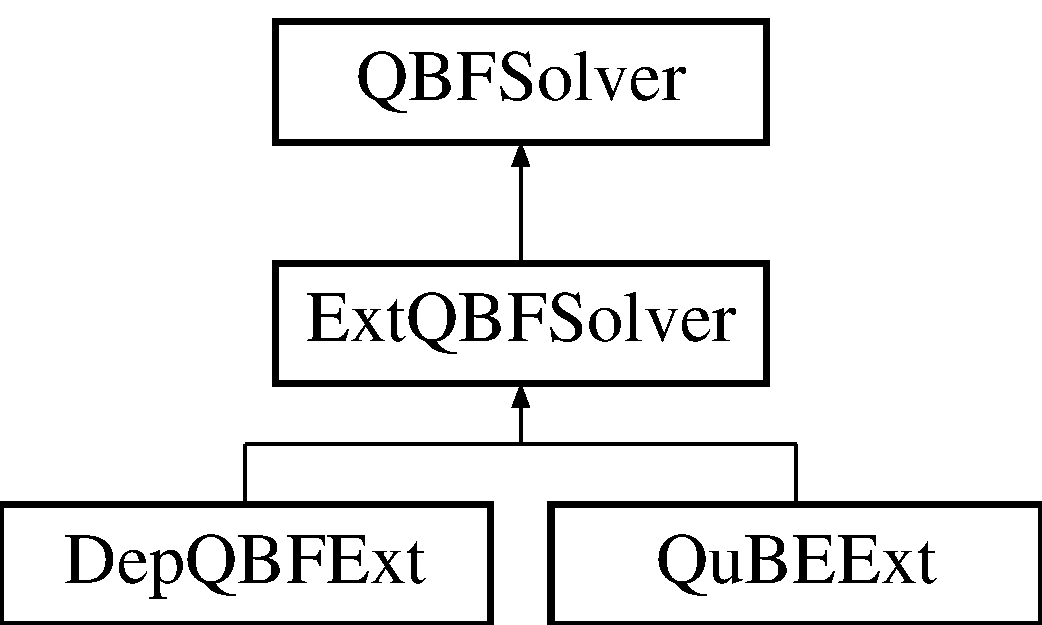
\includegraphics[height=3.000000cm]{classExtQBFSolver}
\end{center}
\end{figure}
\subsection*{Public Types}
\begin{DoxyCompactItemize}
\item 
enum \hyperlink{classQBFSolver_ac091e263cb55286cc07b2451bcf4d3c7}{Quant} \{ \hyperlink{classQBFSolver_ac091e263cb55286cc07b2451bcf4d3c7a090ab4a5b262710ccd80e97d72f9a7b3}{E}, 
\hyperlink{classQBFSolver_ac091e263cb55286cc07b2451bcf4d3c7afd6518d5d985aa8346ac071e4c0d8ee0}{A}
 \}
\begin{DoxyCompactList}\small\item\em A type for the different kinds of quantifiers. \end{DoxyCompactList}\end{DoxyCompactItemize}
\subsection*{Public Member Functions}
\begin{DoxyCompactItemize}
\item 
\hyperlink{classExtQBFSolver_aab51d0c8b2f2e1459247fe6183a31918}{Ext\-Q\-B\-F\-Solver} ()
\begin{DoxyCompactList}\small\item\em Constructor. \end{DoxyCompactList}\item 
virtual \hyperlink{classExtQBFSolver_a02cbc680022daebfb4c08ad40c06999e}{$\sim$\-Ext\-Q\-B\-F\-Solver} ()
\begin{DoxyCompactList}\small\item\em Destructor. \end{DoxyCompactList}\item 
virtual bool \hyperlink{classExtQBFSolver_abec25b97170b79b42b85d1d4ec825a39}{is\-Sat} (const vector$<$ pair$<$ \hyperlink{classVarInfo_a64d1da76cf84fe674e5fef9764ef11cf}{Var\-Info\-::\-Var\-Kind}, \hyperlink{classQBFSolver_ac091e263cb55286cc07b2451bcf4d3c7}{Quant} $>$ $>$ \&quantifier\-\_\-prefix, const \hyperlink{classCNF}{C\-N\-F} \&cnf)
\begin{DoxyCompactList}\small\item\em Checks if a given Q\-B\-F is satisfiable (with quantification over variable kinds). \end{DoxyCompactList}\item 
virtual bool \hyperlink{classExtQBFSolver_adc1bacec3307200dd90b260789e4c808}{is\-Sat} (const vector$<$ pair$<$ vector$<$ int $>$, \hyperlink{classQBFSolver_ac091e263cb55286cc07b2451bcf4d3c7}{Quant} $>$ $>$ \&quantifier\-\_\-prefix, const \hyperlink{classCNF}{C\-N\-F} \&cnf)
\begin{DoxyCompactList}\small\item\em Checks if a given Q\-B\-F is satisfiable (with quantification over variable sets). \end{DoxyCompactList}\item 
virtual bool \hyperlink{classExtQBFSolver_ad66c53343ce9c03eea6e4b5e7753f1b3}{is\-Sat\-Model} (const vector$<$ pair$<$ \hyperlink{classVarInfo_a64d1da76cf84fe674e5fef9764ef11cf}{Var\-Info\-::\-Var\-Kind}, \hyperlink{classQBFSolver_ac091e263cb55286cc07b2451bcf4d3c7}{Quant} $>$ $>$ \&quantifier\-\_\-prefix, const \hyperlink{classCNF}{C\-N\-F} \&cnf, vector$<$ int $>$ \&model)
\begin{DoxyCompactList}\small\item\em Checks satisfiability and extracts a model (quantifying over variable kinds). \end{DoxyCompactList}\item 
virtual bool \hyperlink{classExtQBFSolver_a3add00496f016c2e60a188ce9daa1da1}{is\-Sat\-Model} (const vector$<$ pair$<$ vector$<$ int $>$, \hyperlink{classQBFSolver_ac091e263cb55286cc07b2451bcf4d3c7}{Quant} $>$ $>$ \&quantifier\-\_\-prefix, const \hyperlink{classCNF}{C\-N\-F} \&cnf, vector$<$ int $>$ \&model)
\begin{DoxyCompactList}\small\item\em Checks satisfiability and extracts a model (quantifying over variable sets). \end{DoxyCompactList}\end{DoxyCompactItemize}
\subsection*{Static Public Member Functions}
\begin{DoxyCompactItemize}
\item 
static void \hyperlink{classExtQBFSolver_abebb2acbb5afd5b205254246f39f3e33}{dump\-Q\-B\-F} (const vector$<$ pair$<$ \hyperlink{classVarInfo_a64d1da76cf84fe674e5fef9764ef11cf}{Var\-Info\-::\-Var\-Kind}, \hyperlink{classQBFSolver_ac091e263cb55286cc07b2451bcf4d3c7}{Quant} $>$ $>$ \&quantifier\-\_\-prefix, const \hyperlink{classCNF}{C\-N\-F} \&cnf, const string \&filename)
\begin{DoxyCompactList}\small\item\em Dumps a Q\-B\-F (quantification over variable kinds) into a file in Q\-D\-I\-M\-A\-C\-S format. \end{DoxyCompactList}\item 
static void \hyperlink{classExtQBFSolver_a7e329d1fdce2cf65390930b01cf3a32b}{dump\-Q\-B\-F} (const vector$<$ pair$<$ vector$<$ int $>$, \hyperlink{classQBFSolver_ac091e263cb55286cc07b2451bcf4d3c7}{Quant} $>$ $>$ \&quantifier\-\_\-prefix, const \hyperlink{classCNF}{C\-N\-F} \&cnf, const string \&filename)
\begin{DoxyCompactList}\small\item\em Dumps a Q\-B\-F (quantification over variable kinds) into a file in Q\-D\-I\-M\-A\-C\-S format. \end{DoxyCompactList}\end{DoxyCompactItemize}
\subsection*{Protected Member Functions}
\begin{DoxyCompactItemize}
\item 
virtual bool \hyperlink{classExtQBFSolver_a11ddbf3980824453238071e8a036f804}{parse\-Answer} (int ret) const 
\begin{DoxyCompactList}\small\item\em Parses the answer of the Q\-B\-F solver to get the satisfiability verdict. \end{DoxyCompactList}\item 
virtual bool \hyperlink{classExtQBFSolver_afe52ff8faa21fbdd850b73e8f8cf9839}{parse\-Model} (int ret, const vector$<$ int $>$ \&get, vector$<$ int $>$ \&model) const 
\begin{DoxyCompactList}\small\item\em Parses the answer of the Q\-B\-F solver to get the satisfiability verdict and a model. \end{DoxyCompactList}\item 
virtual void \hyperlink{classExtQBFSolver_a3ee48837c5e937e4d3a5b3c2a6b761d3}{cleanup} ()
\begin{DoxyCompactList}\small\item\em Deletes the temporary files that have been used for communication. \end{DoxyCompactList}\item 
virtual string \hyperlink{classExtQBFSolver_aec4c2d830f72283e2fbabf4a3f62a640}{get\-Solver\-Command} () const =0
\begin{DoxyCompactList}\small\item\em Returns the command to start the solver if no model is needed. \end{DoxyCompactList}\item 
virtual string \hyperlink{classExtQBFSolver_ac2bc9e4817cfa1a54195d7d9f1c7d3bd}{get\-Solver\-Command\-Model} () const =0
\begin{DoxyCompactList}\small\item\em Returns the command to start the solver if a model is needed. \end{DoxyCompactList}\end{DoxyCompactItemize}
\subsection*{Protected Attributes}
\begin{DoxyCompactItemize}
\item 
string \hyperlink{classExtQBFSolver_a04d2ff483c22a11344e46d66ae7e76b1}{in\-\_\-file\-\_\-name\-\_\-}
\begin{DoxyCompactList}\small\item\em The name of the Q\-D\-I\-M\-A\-C\-S file containing the Q\-B\-F to be solved. \end{DoxyCompactList}\item 
string \hyperlink{classExtQBFSolver_a0efb35aa9b807dec521ad3406eaf664d}{out\-\_\-file\-\_\-name\-\_\-}
\begin{DoxyCompactList}\small\item\em The name of the file that is produced by the Q\-B\-F-\/solver (containing the model). \end{DoxyCompactList}\end{DoxyCompactItemize}
\subsection*{Private Member Functions}
\begin{DoxyCompactItemize}
\item 
\hyperlink{classExtQBFSolver_a8ae0e96c56f9e2db776e67ba319d2536}{Ext\-Q\-B\-F\-Solver} (const \hyperlink{classExtQBFSolver}{Ext\-Q\-B\-F\-Solver} \&other)
\begin{DoxyCompactList}\small\item\em Copy constructor. \end{DoxyCompactList}\item 
\hyperlink{classExtQBFSolver}{Ext\-Q\-B\-F\-Solver} \& \hyperlink{classExtQBFSolver_ae0d0f2a04590eec266f65f64ec7e243c}{operator=} (const \hyperlink{classExtQBFSolver}{Ext\-Q\-B\-F\-Solver} \&other)
\begin{DoxyCompactList}\small\item\em Assignment operator. \end{DoxyCompactList}\end{DoxyCompactItemize}


\subsection{Detailed Description}
A generic interface to Q\-B\-F-\/solvers started as external processes. 

This is an abstract base class for all interfaces to Q\-B\-F-\/solvers which start the Q\-B\-F-\/solver in a separate process. Practically all Q\-B\-F-\/solvers understand the Q\-D\-I\-M\-A\-C\-S format as input. Hence, different Q\-B\-F-\/solvers can be interfaced in the same way. The only things that differ from solver to solver are the location of the executable and the command-\/line options that must be set. These solver-\/specific aspects are handled in the derived classes (by overriding certain methods). Everything else is handled in this abstract base class. At he moment there are two implementations of this abstract class\-: \hyperlink{classDepQBFExt}{Dep\-Q\-B\-F\-Ext} and \hyperlink{classQuBEExt}{Qu\-B\-E\-Ext}.

\begin{DoxyAuthor}{Author}
Robert Koenighofer (\href{mailto:robert.koenighofer@iaik.tugraz.at}{\tt robert.\-koenighofer@iaik.\-tugraz.\-at}) 
\end{DoxyAuthor}
\begin{DoxyVersion}{Version}
1.\-2.\-0 
\end{DoxyVersion}


Definition at line 53 of file Ext\-Q\-B\-F\-Solver.\-h.



\subsection{Member Enumeration Documentation}
\hypertarget{classQBFSolver_ac091e263cb55286cc07b2451bcf4d3c7}{\index{Ext\-Q\-B\-F\-Solver@{Ext\-Q\-B\-F\-Solver}!Quant@{Quant}}
\index{Quant@{Quant}!ExtQBFSolver@{Ext\-Q\-B\-F\-Solver}}
\subsubsection[{Quant}]{\setlength{\rightskip}{0pt plus 5cm}enum {\bf Q\-B\-F\-Solver\-::\-Quant}\hspace{0.3cm}{\ttfamily [inherited]}}}\label{classQBFSolver_ac091e263cb55286cc07b2451bcf4d3c7}


A type for the different kinds of quantifiers. 

\begin{Desc}
\item[Enumerator]\par
\begin{description}
\index{E@{E}!Ext\-Q\-B\-F\-Solver@{Ext\-Q\-B\-F\-Solver}}\index{Ext\-Q\-B\-F\-Solver@{Ext\-Q\-B\-F\-Solver}!E@{E}}\item[{\em 
\hypertarget{classQBFSolver_ac091e263cb55286cc07b2451bcf4d3c7a090ab4a5b262710ccd80e97d72f9a7b3}{E}\label{classQBFSolver_ac091e263cb55286cc07b2451bcf4d3c7a090ab4a5b262710ccd80e97d72f9a7b3}
}]The value for existential quantification. \index{A@{A}!Ext\-Q\-B\-F\-Solver@{Ext\-Q\-B\-F\-Solver}}\index{Ext\-Q\-B\-F\-Solver@{Ext\-Q\-B\-F\-Solver}!A@{A}}\item[{\em 
\hypertarget{classQBFSolver_ac091e263cb55286cc07b2451bcf4d3c7afd6518d5d985aa8346ac071e4c0d8ee0}{A}\label{classQBFSolver_ac091e263cb55286cc07b2451bcf4d3c7afd6518d5d985aa8346ac071e4c0d8ee0}
}]The value for universal quantification. \end{description}
\end{Desc}


Definition at line 56 of file Q\-B\-F\-Solver.\-h.



\subsection{Constructor \& Destructor Documentation}
\hypertarget{classExtQBFSolver_aab51d0c8b2f2e1459247fe6183a31918}{\index{Ext\-Q\-B\-F\-Solver@{Ext\-Q\-B\-F\-Solver}!Ext\-Q\-B\-F\-Solver@{Ext\-Q\-B\-F\-Solver}}
\index{Ext\-Q\-B\-F\-Solver@{Ext\-Q\-B\-F\-Solver}!ExtQBFSolver@{Ext\-Q\-B\-F\-Solver}}
\subsubsection[{Ext\-Q\-B\-F\-Solver}]{\setlength{\rightskip}{0pt plus 5cm}Ext\-Q\-B\-F\-Solver\-::\-Ext\-Q\-B\-F\-Solver (
\begin{DoxyParamCaption}
{}
\end{DoxyParamCaption}
)}}\label{classExtQBFSolver_aab51d0c8b2f2e1459247fe6183a31918}


Constructor. 



Definition at line 38 of file Ext\-Q\-B\-F\-Solver.\-cpp.



References Options\-::get\-Tmp\-Dir\-Name(), Options\-::get\-Unique\-Tmp\-File\-Name(), in\-\_\-file\-\_\-name\-\_\-, Options\-::instance(), and out\-\_\-file\-\_\-name\-\_\-.

\hypertarget{classExtQBFSolver_a02cbc680022daebfb4c08ad40c06999e}{\index{Ext\-Q\-B\-F\-Solver@{Ext\-Q\-B\-F\-Solver}!$\sim$\-Ext\-Q\-B\-F\-Solver@{$\sim$\-Ext\-Q\-B\-F\-Solver}}
\index{$\sim$\-Ext\-Q\-B\-F\-Solver@{$\sim$\-Ext\-Q\-B\-F\-Solver}!ExtQBFSolver@{Ext\-Q\-B\-F\-Solver}}
\subsubsection[{$\sim$\-Ext\-Q\-B\-F\-Solver}]{\setlength{\rightskip}{0pt plus 5cm}Ext\-Q\-B\-F\-Solver\-::$\sim$\-Ext\-Q\-B\-F\-Solver (
\begin{DoxyParamCaption}
{}
\end{DoxyParamCaption}
)\hspace{0.3cm}{\ttfamily [virtual]}}}\label{classExtQBFSolver_a02cbc680022daebfb4c08ad40c06999e}


Destructor. 



Definition at line 48 of file Ext\-Q\-B\-F\-Solver.\-cpp.

\hypertarget{classExtQBFSolver_a8ae0e96c56f9e2db776e67ba319d2536}{\index{Ext\-Q\-B\-F\-Solver@{Ext\-Q\-B\-F\-Solver}!Ext\-Q\-B\-F\-Solver@{Ext\-Q\-B\-F\-Solver}}
\index{Ext\-Q\-B\-F\-Solver@{Ext\-Q\-B\-F\-Solver}!ExtQBFSolver@{Ext\-Q\-B\-F\-Solver}}
\subsubsection[{Ext\-Q\-B\-F\-Solver}]{\setlength{\rightskip}{0pt plus 5cm}Ext\-Q\-B\-F\-Solver\-::\-Ext\-Q\-B\-F\-Solver (
\begin{DoxyParamCaption}
\item[{const {\bf Ext\-Q\-B\-F\-Solver} \&}]{other}
\end{DoxyParamCaption}
)\hspace{0.3cm}{\ttfamily [private]}}}\label{classExtQBFSolver_a8ae0e96c56f9e2db776e67ba319d2536}


Copy constructor. 

The copy constructor is disabled (set private) and not implemented.


\begin{DoxyParams}{Parameters}
{\em other} & The source for creating the copy. \\
\hline
\end{DoxyParams}


\subsection{Member Function Documentation}
\hypertarget{classExtQBFSolver_a3ee48837c5e937e4d3a5b3c2a6b761d3}{\index{Ext\-Q\-B\-F\-Solver@{Ext\-Q\-B\-F\-Solver}!cleanup@{cleanup}}
\index{cleanup@{cleanup}!ExtQBFSolver@{Ext\-Q\-B\-F\-Solver}}
\subsubsection[{cleanup}]{\setlength{\rightskip}{0pt plus 5cm}void Ext\-Q\-B\-F\-Solver\-::cleanup (
\begin{DoxyParamCaption}
{}
\end{DoxyParamCaption}
)\hspace{0.3cm}{\ttfamily [protected]}, {\ttfamily [virtual]}}}\label{classExtQBFSolver_a3ee48837c5e937e4d3a5b3c2a6b761d3}


Deletes the temporary files that have been used for communication. 



Definition at line 217 of file Ext\-Q\-B\-F\-Solver.\-cpp.



References in\-\_\-file\-\_\-name\-\_\-, and out\-\_\-file\-\_\-name\-\_\-.



Referenced by is\-Sat(), is\-Sat\-Model(), and Dep\-Q\-B\-F\-Ext\-::qbf\-Cert().

\hypertarget{classExtQBFSolver_abebb2acbb5afd5b205254246f39f3e33}{\index{Ext\-Q\-B\-F\-Solver@{Ext\-Q\-B\-F\-Solver}!dump\-Q\-B\-F@{dump\-Q\-B\-F}}
\index{dump\-Q\-B\-F@{dump\-Q\-B\-F}!ExtQBFSolver@{Ext\-Q\-B\-F\-Solver}}
\subsubsection[{dump\-Q\-B\-F}]{\setlength{\rightskip}{0pt plus 5cm}void Ext\-Q\-B\-F\-Solver\-::dump\-Q\-B\-F (
\begin{DoxyParamCaption}
\item[{const vector$<$ pair$<$ {\bf Var\-Info\-::\-Var\-Kind}, {\bf Quant} $>$ $>$ \&}]{quantifier\-\_\-prefix, }
\item[{const {\bf C\-N\-F} \&}]{cnf, }
\item[{const string \&}]{filename}
\end{DoxyParamCaption}
)\hspace{0.3cm}{\ttfamily [static]}}}\label{classExtQBFSolver_abebb2acbb5afd5b205254246f39f3e33}


Dumps a Q\-B\-F (quantification over variable kinds) into a file in Q\-D\-I\-M\-A\-C\-S format. 


\begin{DoxyParams}{Parameters}
{\em quantifier\-\_\-prefix} & The quantifier prefix as a vector of pairs. vector\mbox{[}0\mbox{]} is the leftmost (i.\-e., outermost) quantifier block. The pairs in the quantifier\-\_\-prefix assign an existential or universal quantifier to every kind of variable that occurs in the cnf. \\
\hline
{\em cnf} & A Boolean formula in \hyperlink{classCNF}{C\-N\-F}. \\
\hline
{\em filename} & The name of the file (including path) to write to. \\
\hline
\end{DoxyParams}


Definition at line 105 of file Ext\-Q\-B\-F\-Solver.\-cpp.



References Q\-B\-F\-Solver\-::\-E, Var\-Manager\-::get\-Max\-C\-N\-F\-Var(), C\-N\-F\-::get\-Nr\-Of\-Clauses(), Var\-Manager\-::get\-Vars\-Of\-Type(), Var\-Manager\-::instance(), and C\-N\-F\-::to\-String().



Referenced by Dep\-Q\-B\-F\-Api\-::debug\-Check\-Bloqqer\-Model(), Dep\-Q\-B\-F\-Api\-::debug\-Check\-Bloqqer\-Verdict(), is\-Sat(), is\-Sat\-Model(), and Dep\-Q\-B\-F\-Ext\-::qbf\-Cert().

\hypertarget{classExtQBFSolver_a7e329d1fdce2cf65390930b01cf3a32b}{\index{Ext\-Q\-B\-F\-Solver@{Ext\-Q\-B\-F\-Solver}!dump\-Q\-B\-F@{dump\-Q\-B\-F}}
\index{dump\-Q\-B\-F@{dump\-Q\-B\-F}!ExtQBFSolver@{Ext\-Q\-B\-F\-Solver}}
\subsubsection[{dump\-Q\-B\-F}]{\setlength{\rightskip}{0pt plus 5cm}void Ext\-Q\-B\-F\-Solver\-::dump\-Q\-B\-F (
\begin{DoxyParamCaption}
\item[{const vector$<$ pair$<$ vector$<$ int $>$, {\bf Quant} $>$ $>$ \&}]{quantifier\-\_\-prefix, }
\item[{const {\bf C\-N\-F} \&}]{cnf, }
\item[{const string \&}]{filename}
\end{DoxyParamCaption}
)\hspace{0.3cm}{\ttfamily [static]}}}\label{classExtQBFSolver_a7e329d1fdce2cf65390930b01cf3a32b}


Dumps a Q\-B\-F (quantification over variable kinds) into a file in Q\-D\-I\-M\-A\-C\-S format. 


\begin{DoxyParams}{Parameters}
{\em quantifier\-\_\-prefix} & The quantifier prefix as a vector of pairs. vector\mbox{[}0\mbox{]} is the leftmost (i.\-e., outermost) quantifier block. The pairs in the quantifier\-\_\-prefix assign an existential or universal quantifier to different sets of variables occurring in the cnf. \\
\hline
{\em cnf} & A Boolean formula in \hyperlink{classCNF}{C\-N\-F}. \\
\hline
{\em filename} & The name of the file (including path) to write to. \\
\hline
\end{DoxyParams}


Definition at line 138 of file Ext\-Q\-B\-F\-Solver.\-cpp.



References Q\-B\-F\-Solver\-::\-E, C\-N\-F\-::get\-Nr\-Of\-Clauses(), and C\-N\-F\-::to\-String().

\hypertarget{classExtQBFSolver_aec4c2d830f72283e2fbabf4a3f62a640}{\index{Ext\-Q\-B\-F\-Solver@{Ext\-Q\-B\-F\-Solver}!get\-Solver\-Command@{get\-Solver\-Command}}
\index{get\-Solver\-Command@{get\-Solver\-Command}!ExtQBFSolver@{Ext\-Q\-B\-F\-Solver}}
\subsubsection[{get\-Solver\-Command}]{\setlength{\rightskip}{0pt plus 5cm}virtual string Ext\-Q\-B\-F\-Solver\-::get\-Solver\-Command (
\begin{DoxyParamCaption}
{}
\end{DoxyParamCaption}
) const\hspace{0.3cm}{\ttfamily [protected]}, {\ttfamily [pure virtual]}}}\label{classExtQBFSolver_aec4c2d830f72283e2fbabf4a3f62a640}


Returns the command to start the solver if no model is needed. 

This command should contain the path to the executable as well as all necessary command line parameters. This method is supposed to be implemented by derived classes.

\begin{DoxyReturn}{Returns}
The command to start the solver if no model is needed. 
\end{DoxyReturn}


Implemented in \hyperlink{classDepQBFExt_a64f0c17958bd64cfd20a1f2478f68077}{Dep\-Q\-B\-F\-Ext}, \hyperlink{classQuBEExt_a2af26a63952d83a50a4bd3d72bfc572a}{Qu\-B\-E\-Ext}, and \hyperlink{classRareqsExt_a063f7edb8cd60f8bf44c0d16c0131166}{Rareqs\-Ext}.



Referenced by is\-Sat().

\hypertarget{classExtQBFSolver_ac2bc9e4817cfa1a54195d7d9f1c7d3bd}{\index{Ext\-Q\-B\-F\-Solver@{Ext\-Q\-B\-F\-Solver}!get\-Solver\-Command\-Model@{get\-Solver\-Command\-Model}}
\index{get\-Solver\-Command\-Model@{get\-Solver\-Command\-Model}!ExtQBFSolver@{Ext\-Q\-B\-F\-Solver}}
\subsubsection[{get\-Solver\-Command\-Model}]{\setlength{\rightskip}{0pt plus 5cm}virtual string Ext\-Q\-B\-F\-Solver\-::get\-Solver\-Command\-Model (
\begin{DoxyParamCaption}
{}
\end{DoxyParamCaption}
) const\hspace{0.3cm}{\ttfamily [protected]}, {\ttfamily [pure virtual]}}}\label{classExtQBFSolver_ac2bc9e4817cfa1a54195d7d9f1c7d3bd}


Returns the command to start the solver if a model is needed. 

This command should contain the path to the executable as well as all necessary command line parameters. This method is supposed to be implemented by derived classes.

\begin{DoxyReturn}{Returns}
The command to start the solver if a model is needed. 
\end{DoxyReturn}


Implemented in \hyperlink{classDepQBFExt_a72321fcf85a52333c0f7e83004a3f119}{Dep\-Q\-B\-F\-Ext}, \hyperlink{classQuBEExt_a846ea873ec83e57213f1931d85cb8bd0}{Qu\-B\-E\-Ext}, and \hyperlink{classRareqsExt_aeab7d75367b08767e6c1e0411b254961}{Rareqs\-Ext}.



Referenced by is\-Sat\-Model().

\hypertarget{classExtQBFSolver_abec25b97170b79b42b85d1d4ec825a39}{\index{Ext\-Q\-B\-F\-Solver@{Ext\-Q\-B\-F\-Solver}!is\-Sat@{is\-Sat}}
\index{is\-Sat@{is\-Sat}!ExtQBFSolver@{Ext\-Q\-B\-F\-Solver}}
\subsubsection[{is\-Sat}]{\setlength{\rightskip}{0pt plus 5cm}bool Ext\-Q\-B\-F\-Solver\-::is\-Sat (
\begin{DoxyParamCaption}
\item[{const vector$<$ pair$<$ {\bf Var\-Info\-::\-Var\-Kind}, {\bf Quant} $>$ $>$ \&}]{quantifier\-\_\-prefix, }
\item[{const {\bf C\-N\-F} \&}]{cnf}
\end{DoxyParamCaption}
)\hspace{0.3cm}{\ttfamily [virtual]}}}\label{classExtQBFSolver_abec25b97170b79b42b85d1d4ec825a39}


Checks if a given Q\-B\-F is satisfiable (with quantification over variable kinds). 

The Q\-B\-F consists of a quantifier prefix and a Boolean formula in \hyperlink{classCNF}{C\-N\-F}. The quantifier prefix assigns an existential or universal quantifier to every kind of variable. The Q\-B\-F is dumped into a file, a Q\-B\-F-\/solver is called, and the exit code is used to infer the satisfiability result.


\begin{DoxyExceptions}{Exceptions}
{\em \hyperlink{classDemiurgeException}{Demiurge\-Exception}} & if the solver crashed or a timeout occurred. \\
\hline
\end{DoxyExceptions}

\begin{DoxyParams}{Parameters}
{\em quantifier\-\_\-prefix} & The quantifier prefix as a vector of pairs. vector\mbox{[}0\mbox{]} is the leftmost (i.\-e., outermost) quantifier block. The pairs in the quantifier\-\_\-prefix assign an existential or universal quantifier to every kind of variable that occurs in the cnf. \\
\hline
{\em cnf} & A Boolean formula in \hyperlink{classCNF}{C\-N\-F}. \\
\hline
\end{DoxyParams}
\begin{DoxyReturn}{Returns}
True if the Q\-B\-F is satisfiable, false otherwise. 
\end{DoxyReturn}


Implements \hyperlink{classQBFSolver_a53ef157391b176dfbd2a77a1e31befc3}{Q\-B\-F\-Solver}.



Definition at line 54 of file Ext\-Q\-B\-F\-Solver.\-cpp.



References cleanup(), dump\-Q\-B\-F(), get\-Solver\-Command(), in\-\_\-file\-\_\-name\-\_\-, and parse\-Answer().



Referenced by Q\-B\-F\-Cert\-Impl\-Extractor\-::run().

\hypertarget{classExtQBFSolver_adc1bacec3307200dd90b260789e4c808}{\index{Ext\-Q\-B\-F\-Solver@{Ext\-Q\-B\-F\-Solver}!is\-Sat@{is\-Sat}}
\index{is\-Sat@{is\-Sat}!ExtQBFSolver@{Ext\-Q\-B\-F\-Solver}}
\subsubsection[{is\-Sat}]{\setlength{\rightskip}{0pt plus 5cm}bool Ext\-Q\-B\-F\-Solver\-::is\-Sat (
\begin{DoxyParamCaption}
\item[{const vector$<$ pair$<$ vector$<$ int $>$, {\bf Quant} $>$ $>$ \&}]{quantifier\-\_\-prefix, }
\item[{const {\bf C\-N\-F} \&}]{cnf}
\end{DoxyParamCaption}
)\hspace{0.3cm}{\ttfamily [virtual]}}}\label{classExtQBFSolver_adc1bacec3307200dd90b260789e4c808}


Checks if a given Q\-B\-F is satisfiable (with quantification over variable sets). 

The Q\-B\-F consists of a quantifier prefix and a Boolean formula in \hyperlink{classCNF}{C\-N\-F}. The quantifier prefix assigns an existential or universal quantifier to different sets variable. The Q\-B\-F is dumped into a file, a Q\-B\-F-\/solver is called, and the exit code is used to infer the satisfiability result.


\begin{DoxyExceptions}{Exceptions}
{\em \hyperlink{classDemiurgeException}{Demiurge\-Exception}} & if the solver crashed or a timeout occurred. \\
\hline
\end{DoxyExceptions}

\begin{DoxyParams}{Parameters}
{\em quantifier\-\_\-prefix} & The quantifier prefix as a vector of pairs. vector\mbox{[}0\mbox{]} is the leftmost (i.\-e., outermost) quantifier block. The pairs in the quantifier\-\_\-prefix assign an existential or universal quantifier to different sets of variables occurring in the cnf. \\
\hline
{\em cnf} & A Boolean formula in \hyperlink{classCNF}{C\-N\-F}. \\
\hline
\end{DoxyParams}
\begin{DoxyReturn}{Returns}
True if the Q\-B\-F is satisfiable, false otherwise. 
\end{DoxyReturn}


Implements \hyperlink{classQBFSolver_aca37de5801e36d4749b80b6c8c2023a9}{Q\-B\-F\-Solver}.



Definition at line 66 of file Ext\-Q\-B\-F\-Solver.\-cpp.



References cleanup(), dump\-Q\-B\-F(), get\-Solver\-Command(), in\-\_\-file\-\_\-name\-\_\-, and parse\-Answer().

\hypertarget{classExtQBFSolver_ad66c53343ce9c03eea6e4b5e7753f1b3}{\index{Ext\-Q\-B\-F\-Solver@{Ext\-Q\-B\-F\-Solver}!is\-Sat\-Model@{is\-Sat\-Model}}
\index{is\-Sat\-Model@{is\-Sat\-Model}!ExtQBFSolver@{Ext\-Q\-B\-F\-Solver}}
\subsubsection[{is\-Sat\-Model}]{\setlength{\rightskip}{0pt plus 5cm}bool Ext\-Q\-B\-F\-Solver\-::is\-Sat\-Model (
\begin{DoxyParamCaption}
\item[{const vector$<$ pair$<$ {\bf Var\-Info\-::\-Var\-Kind}, {\bf Quant} $>$ $>$ \&}]{quantifier\-\_\-prefix, }
\item[{const {\bf C\-N\-F} \&}]{cnf, }
\item[{vector$<$ int $>$ \&}]{model}
\end{DoxyParamCaption}
)\hspace{0.3cm}{\ttfamily [virtual]}}}\label{classExtQBFSolver_ad66c53343ce9c03eea6e4b5e7753f1b3}


Checks satisfiability and extracts a model (quantifying over variable kinds). 

Just like \hyperlink{classExtQBFSolver_abec25b97170b79b42b85d1d4ec825a39}{is\-Sat() }, this method checks a quantified Boolean formula for satisfiability. If the Q\-B\-F is satisfiable, this method also extracts a model (a satisfying assignment) for all variables which are quantified existentially on the outermost level. The model is provided as cube\-: negated variables in the cube are F\-A\-L\-S\-E, unnegated ones are T\-R\-U\-E.


\begin{DoxyExceptions}{Exceptions}
{\em \hyperlink{classDemiurgeException}{Demiurge\-Exception}} & if the solver crashed or a timeout occurred. \\
\hline
\end{DoxyExceptions}

\begin{DoxyParams}{Parameters}
{\em quantifier\-\_\-prefix} & The quantifier prefix as a vector of pairs. vector\mbox{[}0\mbox{]} is the leftmost (i.\-e., outermost) quantifier block. The pairs in the quantifier\-\_\-prefix assign an existential or universal quantifier to every kind of variable that occurs in the cnf. \\
\hline
{\em cnf} & A Boolean formula in \hyperlink{classCNF}{C\-N\-F}. \\
\hline
{\em model} & The resulting model in form of a cube in case of satisfiability. Negated variables in the cube are F\-A\-L\-S\-E, unnegated ones are T\-R\-U\-E. If the formula is unsatisfiable (this method returns false) then this parameter is not modified. \\
\hline
\end{DoxyParams}
\begin{DoxyReturn}{Returns}
True if the Q\-B\-F is satisfiable, false otherwise. 
\end{DoxyReturn}


Implements \hyperlink{classQBFSolver_a76fc0c757a2c039816e3e06547f06d5c}{Q\-B\-F\-Solver}.



Definition at line 78 of file Ext\-Q\-B\-F\-Solver.\-cpp.



References cleanup(), dump\-Q\-B\-F(), get\-Solver\-Command\-Model(), Var\-Manager\-::get\-Vars\-Of\-Type(), in\-\_\-file\-\_\-name\-\_\-, Var\-Manager\-::instance(), and parse\-Model().



Referenced by Templ\-Explorer\-::synt\-Q\-B\-F().

\hypertarget{classExtQBFSolver_a3add00496f016c2e60a188ce9daa1da1}{\index{Ext\-Q\-B\-F\-Solver@{Ext\-Q\-B\-F\-Solver}!is\-Sat\-Model@{is\-Sat\-Model}}
\index{is\-Sat\-Model@{is\-Sat\-Model}!ExtQBFSolver@{Ext\-Q\-B\-F\-Solver}}
\subsubsection[{is\-Sat\-Model}]{\setlength{\rightskip}{0pt plus 5cm}bool Ext\-Q\-B\-F\-Solver\-::is\-Sat\-Model (
\begin{DoxyParamCaption}
\item[{const vector$<$ pair$<$ vector$<$ int $>$, {\bf Quant} $>$ $>$ \&}]{quantifier\-\_\-prefix, }
\item[{const {\bf C\-N\-F} \&}]{cnf, }
\item[{vector$<$ int $>$ \&}]{model}
\end{DoxyParamCaption}
)\hspace{0.3cm}{\ttfamily [virtual]}}}\label{classExtQBFSolver_a3add00496f016c2e60a188ce9daa1da1}


Checks satisfiability and extracts a model (quantifying over variable sets). 

Just like \hyperlink{classExtQBFSolver_abec25b97170b79b42b85d1d4ec825a39}{is\-Sat() }, this method checks a quantified Boolean formula for satisfiability. If the Q\-B\-F is satisfiable, this method also extracts a model (a satisfying assignment) for all variables which are quantified existentially on the outermost level. The model is provided as cube\-: negated variables in the cube are F\-A\-L\-S\-E, unnegated ones are T\-R\-U\-E.


\begin{DoxyExceptions}{Exceptions}
{\em \hyperlink{classDemiurgeException}{Demiurge\-Exception}} & if the solver crashed or a timeout occurred. \\
\hline
\end{DoxyExceptions}

\begin{DoxyParams}{Parameters}
{\em quantifier\-\_\-prefix} & The quantifier prefix as a vector of pairs. vector\mbox{[}0\mbox{]} is the leftmost (i.\-e., outermost) quantifier block. The pairs in the quantifier\-\_\-prefix assign an existential or universal quantifier to different sets of variables occurring in the cnf. \\
\hline
{\em cnf} & A Boolean formula in \hyperlink{classCNF}{C\-N\-F}. \\
\hline
{\em model} & The resulting model in form of a cube in case of satisfiability. Negated variables in the cube are F\-A\-L\-S\-E, unnegated ones are T\-R\-U\-E. If the formula is unsatisfiable (this method returns false) then this parameter is not modified. \\
\hline
\end{DoxyParams}
\begin{DoxyReturn}{Returns}
True if the Q\-B\-F is satisfiable, false otherwise. 
\end{DoxyReturn}


Implements \hyperlink{classQBFSolver_a12f2ce57b778b9efe729d63bf881493d}{Q\-B\-F\-Solver}.



Definition at line 92 of file Ext\-Q\-B\-F\-Solver.\-cpp.



References cleanup(), dump\-Q\-B\-F(), get\-Solver\-Command\-Model(), in\-\_\-file\-\_\-name\-\_\-, and parse\-Model().

\hypertarget{classExtQBFSolver_ae0d0f2a04590eec266f65f64ec7e243c}{\index{Ext\-Q\-B\-F\-Solver@{Ext\-Q\-B\-F\-Solver}!operator=@{operator=}}
\index{operator=@{operator=}!ExtQBFSolver@{Ext\-Q\-B\-F\-Solver}}
\subsubsection[{operator=}]{\setlength{\rightskip}{0pt plus 5cm}{\bf Ext\-Q\-B\-F\-Solver}\& Ext\-Q\-B\-F\-Solver\-::operator= (
\begin{DoxyParamCaption}
\item[{const {\bf Ext\-Q\-B\-F\-Solver} \&}]{other}
\end{DoxyParamCaption}
)\hspace{0.3cm}{\ttfamily [private]}}}\label{classExtQBFSolver_ae0d0f2a04590eec266f65f64ec7e243c}


Assignment operator. 

The assignment operator is disabled (set private) and not implemented.


\begin{DoxyParams}{Parameters}
{\em other} & The source for creating the copy. \\
\hline
\end{DoxyParams}
\begin{DoxyReturn}{Returns}
The result of the assignment, i.\-e, $\ast$this. 
\end{DoxyReturn}
\hypertarget{classExtQBFSolver_a11ddbf3980824453238071e8a036f804}{\index{Ext\-Q\-B\-F\-Solver@{Ext\-Q\-B\-F\-Solver}!parse\-Answer@{parse\-Answer}}
\index{parse\-Answer@{parse\-Answer}!ExtQBFSolver@{Ext\-Q\-B\-F\-Solver}}
\subsubsection[{parse\-Answer}]{\setlength{\rightskip}{0pt plus 5cm}bool Ext\-Q\-B\-F\-Solver\-::parse\-Answer (
\begin{DoxyParamCaption}
\item[{int}]{ret}
\end{DoxyParamCaption}
) const\hspace{0.3cm}{\ttfamily [protected]}, {\ttfamily [virtual]}}}\label{classExtQBFSolver_a11ddbf3980824453238071e8a036f804}


Parses the answer of the Q\-B\-F solver to get the satisfiability verdict. 


\begin{DoxyExceptions}{Exceptions}
{\em \hyperlink{classDemiurgeException}{Demiurge\-Exception}} & if the solver crashed or a timeout occurred. \\
\hline
\end{DoxyExceptions}

\begin{DoxyParams}{Parameters}
{\em ret} & The exit code of the process running the Q\-B\-F solver. \\
\hline
\end{DoxyParams}
\begin{DoxyReturn}{Returns}
True in case of satisfiability, false for unsatisfiability. 
\end{DoxyReturn}


Definition at line 180 of file Ext\-Q\-B\-F\-Solver.\-cpp.



Referenced by is\-Sat().

\hypertarget{classExtQBFSolver_afe52ff8faa21fbdd850b73e8f8cf9839}{\index{Ext\-Q\-B\-F\-Solver@{Ext\-Q\-B\-F\-Solver}!parse\-Model@{parse\-Model}}
\index{parse\-Model@{parse\-Model}!ExtQBFSolver@{Ext\-Q\-B\-F\-Solver}}
\subsubsection[{parse\-Model}]{\setlength{\rightskip}{0pt plus 5cm}bool Ext\-Q\-B\-F\-Solver\-::parse\-Model (
\begin{DoxyParamCaption}
\item[{int}]{ret, }
\item[{const vector$<$ int $>$ \&}]{get, }
\item[{vector$<$ int $>$ \&}]{model}
\end{DoxyParamCaption}
) const\hspace{0.3cm}{\ttfamily [protected]}, {\ttfamily [virtual]}}}\label{classExtQBFSolver_afe52ff8faa21fbdd850b73e8f8cf9839}


Parses the answer of the Q\-B\-F solver to get the satisfiability verdict and a model. 


\begin{DoxyExceptions}{Exceptions}
{\em \hyperlink{classDemiurgeException}{Demiurge\-Exception}} & if the solver crashed or a timeout occurred. \\
\hline
\end{DoxyExceptions}

\begin{DoxyParams}{Parameters}
{\em ret} & The exit code of the process running the Q\-B\-F solver. \\
\hline
{\em get} & The variables of interest for which we want to have a satisfying assignment. \\
\hline
{\em model} & An empty vector. In case of satisfiability, this method will write a satisfying assignment in form of a cube into this vector. \\
\hline
\end{DoxyParams}
\begin{DoxyReturn}{Returns}
True in case of satisfiability, false for unsatisfiability. 
\end{DoxyReturn}


Reimplemented in \hyperlink{classDepQBFExt_a9dd5f30054b19543393c43796ac43016}{Dep\-Q\-B\-F\-Ext}.



Definition at line 190 of file Ext\-Q\-B\-F\-Solver.\-cpp.



References M\-A\-S\-S\-E\-R\-T, out\-\_\-file\-\_\-name\-\_\-, and File\-Utils\-::read\-File().



Referenced by is\-Sat\-Model().



\subsection{Member Data Documentation}
\hypertarget{classExtQBFSolver_a04d2ff483c22a11344e46d66ae7e76b1}{\index{Ext\-Q\-B\-F\-Solver@{Ext\-Q\-B\-F\-Solver}!in\-\_\-file\-\_\-name\-\_\-@{in\-\_\-file\-\_\-name\-\_\-}}
\index{in\-\_\-file\-\_\-name\-\_\-@{in\-\_\-file\-\_\-name\-\_\-}!ExtQBFSolver@{Ext\-Q\-B\-F\-Solver}}
\subsubsection[{in\-\_\-file\-\_\-name\-\_\-}]{\setlength{\rightskip}{0pt plus 5cm}string Ext\-Q\-B\-F\-Solver\-::in\-\_\-file\-\_\-name\-\_\-\hspace{0.3cm}{\ttfamily [protected]}}}\label{classExtQBFSolver_a04d2ff483c22a11344e46d66ae7e76b1}


The name of the Q\-D\-I\-M\-A\-C\-S file containing the Q\-B\-F to be solved. 



Definition at line 232 of file Ext\-Q\-B\-F\-Solver.\-h.



Referenced by cleanup(), Ext\-Q\-B\-F\-Solver(), Rareqs\-Ext\-::get\-Solver\-Command(), Qu\-B\-E\-Ext\-::get\-Solver\-Command(), Dep\-Q\-B\-F\-Ext\-::get\-Solver\-Command(), Rareqs\-Ext\-::get\-Solver\-Command\-Model(), Qu\-B\-E\-Ext\-::get\-Solver\-Command\-Model(), Dep\-Q\-B\-F\-Ext\-::get\-Solver\-Command\-Model(), is\-Sat(), is\-Sat\-Model(), and Dep\-Q\-B\-F\-Ext\-::qbf\-Cert().

\hypertarget{classExtQBFSolver_a0efb35aa9b807dec521ad3406eaf664d}{\index{Ext\-Q\-B\-F\-Solver@{Ext\-Q\-B\-F\-Solver}!out\-\_\-file\-\_\-name\-\_\-@{out\-\_\-file\-\_\-name\-\_\-}}
\index{out\-\_\-file\-\_\-name\-\_\-@{out\-\_\-file\-\_\-name\-\_\-}!ExtQBFSolver@{Ext\-Q\-B\-F\-Solver}}
\subsubsection[{out\-\_\-file\-\_\-name\-\_\-}]{\setlength{\rightskip}{0pt plus 5cm}string Ext\-Q\-B\-F\-Solver\-::out\-\_\-file\-\_\-name\-\_\-\hspace{0.3cm}{\ttfamily [protected]}}}\label{classExtQBFSolver_a0efb35aa9b807dec521ad3406eaf664d}


The name of the file that is produced by the Q\-B\-F-\/solver (containing the model). 



Definition at line 237 of file Ext\-Q\-B\-F\-Solver.\-h.



Referenced by cleanup(), Ext\-Q\-B\-F\-Solver(), Rareqs\-Ext\-::get\-Solver\-Command(), Qu\-B\-E\-Ext\-::get\-Solver\-Command(), Dep\-Q\-B\-F\-Ext\-::get\-Solver\-Command(), Rareqs\-Ext\-::get\-Solver\-Command\-Model(), Qu\-B\-E\-Ext\-::get\-Solver\-Command\-Model(), Dep\-Q\-B\-F\-Ext\-::get\-Solver\-Command\-Model(), Rareqs\-Ext\-::parse\-Model(), Dep\-Q\-B\-F\-Ext\-::parse\-Model(), and parse\-Model().



The documentation for this class was generated from the following files\-:\begin{DoxyCompactItemize}
\item 
src/\hyperlink{ExtQBFSolver_8h}{Ext\-Q\-B\-F\-Solver.\-h}\item 
src/\hyperlink{ExtQBFSolver_8cpp}{Ext\-Q\-B\-F\-Solver.\-cpp}\end{DoxyCompactItemize}

\hypertarget{classFileUtils}{\section{File\-Utils Class Reference}
\label{classFileUtils}\index{File\-Utils@{File\-Utils}}
}


Contains utility functions for access to files.  




{\ttfamily \#include $<$File\-Utils.\-h$>$}

\subsection*{Public Member Functions}
\begin{DoxyCompactItemize}
\item 
virtual \hyperlink{classFileUtils_a113a3a0ae84133a66408b20da027c0c7}{$\sim$\-File\-Utils} ()
\begin{DoxyCompactList}\small\item\em Destructor. \end{DoxyCompactList}\end{DoxyCompactItemize}
\subsection*{Static Public Member Functions}
\begin{DoxyCompactItemize}
\item 
static bool \hyperlink{classFileUtils_aa4a1c5a23271a5c284541504fffd2ba6}{file\-Exists} (const string \&file\-\_\-name)
\begin{DoxyCompactList}\small\item\em Checks if a file exists. \end{DoxyCompactList}\item 
static bool \hyperlink{classFileUtils_a1079af04bf2282d524df691ac8124879}{read\-File} (const string \&file\-\_\-name, string \&file\-\_\-content)
\begin{DoxyCompactList}\small\item\em Reads the content of a file into a string. \end{DoxyCompactList}\item 
static bool \hyperlink{classFileUtils_a812ab360ba9b90eb50c73f95e7e001ba}{write\-File} (const string \&file\-\_\-name, const string \&file\-\_\-content)
\begin{DoxyCompactList}\small\item\em Writes the content of a string into a file. \end{DoxyCompactList}\end{DoxyCompactItemize}
\subsection*{Private Member Functions}
\begin{DoxyCompactItemize}
\item 
\hyperlink{classFileUtils_abb87f1bbabb1164634e428aee3559b10}{File\-Utils} ()
\begin{DoxyCompactList}\small\item\em Constructor. \end{DoxyCompactList}\item 
\hyperlink{classFileUtils_a0453599aa15cd007a27422bd74dd84c8}{File\-Utils} (const \hyperlink{classFileUtils}{File\-Utils} \&other)
\begin{DoxyCompactList}\small\item\em Copy constructor. \end{DoxyCompactList}\item 
\hyperlink{classFileUtils}{File\-Utils} \& \hyperlink{classFileUtils_a588f4d21844dbaf5275512e65c846781}{operator=} (const \hyperlink{classFileUtils}{File\-Utils} \&other)
\begin{DoxyCompactList}\small\item\em Assignment operator. \end{DoxyCompactList}\end{DoxyCompactItemize}


\subsection{Detailed Description}
Contains utility functions for access to files. 

\begin{DoxyAuthor}{Author}
Robert Koenighofer (\href{mailto:robert.koenighofer@iaik.tugraz.at}{\tt robert.\-koenighofer@iaik.\-tugraz.\-at}) 
\end{DoxyAuthor}
\begin{DoxyVersion}{Version}
1.\-1.\-0 
\end{DoxyVersion}


Definition at line 42 of file File\-Utils.\-h.



\subsection{Constructor \& Destructor Documentation}
\hypertarget{classFileUtils_a113a3a0ae84133a66408b20da027c0c7}{\index{File\-Utils@{File\-Utils}!$\sim$\-File\-Utils@{$\sim$\-File\-Utils}}
\index{$\sim$\-File\-Utils@{$\sim$\-File\-Utils}!FileUtils@{File\-Utils}}
\subsubsection[{$\sim$\-File\-Utils}]{\setlength{\rightskip}{0pt plus 5cm}File\-Utils\-::$\sim$\-File\-Utils (
\begin{DoxyParamCaption}
{}
\end{DoxyParamCaption}
)\hspace{0.3cm}{\ttfamily [virtual]}}}\label{classFileUtils_a113a3a0ae84133a66408b20da027c0c7}


Destructor. 



Definition at line 85 of file File\-Utils.\-cpp.

\hypertarget{classFileUtils_abb87f1bbabb1164634e428aee3559b10}{\index{File\-Utils@{File\-Utils}!File\-Utils@{File\-Utils}}
\index{File\-Utils@{File\-Utils}!FileUtils@{File\-Utils}}
\subsubsection[{File\-Utils}]{\setlength{\rightskip}{0pt plus 5cm}File\-Utils\-::\-File\-Utils (
\begin{DoxyParamCaption}
{}
\end{DoxyParamCaption}
)\hspace{0.3cm}{\ttfamily [private]}}}\label{classFileUtils_abb87f1bbabb1164634e428aee3559b10}


Constructor. 

The constructor is private and not implemented. Use the static methods. \hypertarget{classFileUtils_a0453599aa15cd007a27422bd74dd84c8}{\index{File\-Utils@{File\-Utils}!File\-Utils@{File\-Utils}}
\index{File\-Utils@{File\-Utils}!FileUtils@{File\-Utils}}
\subsubsection[{File\-Utils}]{\setlength{\rightskip}{0pt plus 5cm}File\-Utils\-::\-File\-Utils (
\begin{DoxyParamCaption}
\item[{const {\bf File\-Utils} \&}]{other}
\end{DoxyParamCaption}
)\hspace{0.3cm}{\ttfamily [private]}}}\label{classFileUtils_a0453599aa15cd007a27422bd74dd84c8}


Copy constructor. 

The copy constructor is disabled (set private) and not implemented.


\begin{DoxyParams}{Parameters}
{\em other} & The source for creating the copy. \\
\hline
\end{DoxyParams}


\subsection{Member Function Documentation}
\hypertarget{classFileUtils_aa4a1c5a23271a5c284541504fffd2ba6}{\index{File\-Utils@{File\-Utils}!file\-Exists@{file\-Exists}}
\index{file\-Exists@{file\-Exists}!FileUtils@{File\-Utils}}
\subsubsection[{file\-Exists}]{\setlength{\rightskip}{0pt plus 5cm}bool File\-Utils\-::file\-Exists (
\begin{DoxyParamCaption}
\item[{const string \&}]{file\-\_\-name}
\end{DoxyParamCaption}
)\hspace{0.3cm}{\ttfamily [static]}}}\label{classFileUtils_aa4a1c5a23271a5c284541504fffd2ba6}


Checks if a file exists. 


\begin{DoxyParams}{Parameters}
{\em file\-\_\-name} & The name of the file to check. \\
\hline
\end{DoxyParams}
\begin{DoxyReturn}{Returns}
True if the file exists (and could be opened), false otherwise. 
\end{DoxyReturn}


Definition at line 33 of file File\-Utils.\-cpp.

\hypertarget{classFileUtils_a588f4d21844dbaf5275512e65c846781}{\index{File\-Utils@{File\-Utils}!operator=@{operator=}}
\index{operator=@{operator=}!FileUtils@{File\-Utils}}
\subsubsection[{operator=}]{\setlength{\rightskip}{0pt plus 5cm}{\bf File\-Utils}\& File\-Utils\-::operator= (
\begin{DoxyParamCaption}
\item[{const {\bf File\-Utils} \&}]{other}
\end{DoxyParamCaption}
)\hspace{0.3cm}{\ttfamily [private]}}}\label{classFileUtils_a588f4d21844dbaf5275512e65c846781}


Assignment operator. 

The assignment operator is disabled (set private) and not implemented.


\begin{DoxyParams}{Parameters}
{\em other} & The source for creating the copy. \\
\hline
\end{DoxyParams}
\begin{DoxyReturn}{Returns}
The result of the assignment, i.\-e, $\ast$this. 
\end{DoxyReturn}
\hypertarget{classFileUtils_a1079af04bf2282d524df691ac8124879}{\index{File\-Utils@{File\-Utils}!read\-File@{read\-File}}
\index{read\-File@{read\-File}!FileUtils@{File\-Utils}}
\subsubsection[{read\-File}]{\setlength{\rightskip}{0pt plus 5cm}bool File\-Utils\-::read\-File (
\begin{DoxyParamCaption}
\item[{const string \&}]{file\-\_\-name, }
\item[{string \&}]{file\-\_\-content}
\end{DoxyParamCaption}
)\hspace{0.3cm}{\ttfamily [static]}}}\label{classFileUtils_a1079af04bf2282d524df691ac8124879}


Reads the content of a file into a string. 


\begin{DoxyParams}{Parameters}
{\em file\-\_\-name} & The name of the file to read. \\
\hline
{\em file\-\_\-content} & The read file content is appended to this string. \\
\hline
\end{DoxyParams}
\begin{DoxyReturn}{Returns}
True if file reading was successful, false otherwise (e.\-g. because the file does not exist, could not be opened, etc.) 
\end{DoxyReturn}


Definition at line 42 of file File\-Utils.\-cpp.



References M\-A\-S\-S\-E\-R\-T.



Referenced by Ext\-Q\-B\-F\-Solver\-::parse\-Model(), and E\-P\-R\-Synthesizer\-::run().

\hypertarget{classFileUtils_a812ab360ba9b90eb50c73f95e7e001ba}{\index{File\-Utils@{File\-Utils}!write\-File@{write\-File}}
\index{write\-File@{write\-File}!FileUtils@{File\-Utils}}
\subsubsection[{write\-File}]{\setlength{\rightskip}{0pt plus 5cm}bool File\-Utils\-::write\-File (
\begin{DoxyParamCaption}
\item[{const string \&}]{file\-\_\-name, }
\item[{const string \&}]{file\-\_\-content}
\end{DoxyParamCaption}
)\hspace{0.3cm}{\ttfamily [static]}}}\label{classFileUtils_a812ab360ba9b90eb50c73f95e7e001ba}


Writes the content of a string into a file. 

If the file already exists, it is overwritten. The directory into which the file should be written must exist.


\begin{DoxyParams}{Parameters}
{\em file\-\_\-name} & The name of the file to write. \\
\hline
{\em file\-\_\-content} & The content to write into this file. \\
\hline
\end{DoxyParams}
\begin{DoxyReturn}{Returns}
True if writing was successful, false otherwise. 
\end{DoxyReturn}


Definition at line 71 of file File\-Utils.\-cpp.



Referenced by E\-P\-R\-Synthesizer\-::run().



The documentation for this class was generated from the following files\-:\begin{DoxyCompactItemize}
\item 
src/\hyperlink{FileUtils_8h}{File\-Utils.\-h}\item 
src/\hyperlink{FileUtils_8cpp}{File\-Utils.\-cpp}\end{DoxyCompactItemize}

\hypertarget{classIFM13Explorer}{\section{I\-F\-M13\-Explorer Class Reference}
\label{classIFM13Explorer}\index{I\-F\-M13\-Explorer@{I\-F\-M13\-Explorer}}
}


Implements the method of \hyperlink{classIFM13Synth}{I\-F\-M13\-Synth} in a parallelized way.  




{\ttfamily \#include $<$Parallel\-Learner.\-h$>$}

\subsection*{Public Member Functions}
\begin{DoxyCompactItemize}
\item 
\hyperlink{classIFM13Explorer_a8830825d1b7347fb02e7a74f7e558e2d}{I\-F\-M13\-Explorer} (\hyperlink{classParallelLearner}{Parallel\-Learner} \&coordinator)
\begin{DoxyCompactList}\small\item\em Constructor. \end{DoxyCompactList}\item 
virtual \hyperlink{classIFM13Explorer_a7334013d4c514c392e0c38ee89a85b76}{$\sim$\-I\-F\-M13\-Explorer} ()
\begin{DoxyCompactList}\small\item\em Destructor. \end{DoxyCompactList}\item 
void \hyperlink{classIFM13Explorer_a19efbbf6644d73d9d7d662b121e3d151}{explore\-Clauses} ()
\begin{DoxyCompactList}\small\item\em The work-\/horse of this class. \end{DoxyCompactList}\item 
void \hyperlink{classIFM13Explorer_a37e60ac394b868d5f375c5b684aeaebc}{notify\-New\-Win\-Reg\-Clause} (const vector$<$ int $>$ \&clause, int src)
\begin{DoxyCompactList}\small\item\em Notifies this worker about a new winning region clause. \end{DoxyCompactList}\end{DoxyCompactItemize}
\subsection*{Protected Member Functions}
\begin{DoxyCompactItemize}
\item 
void \hyperlink{classIFM13Explorer_ae2e510e5b13e7166c5d6170a286a7295}{consider\-New\-Info\-From\-Others} ()
\begin{DoxyCompactList}\small\item\em Considers new winning region clauses that have been found by other threads. \end{DoxyCompactList}\item 
size\-\_\-t \hyperlink{classIFM13Explorer_a52595f5290210c0a79b45c9a077abdb2}{propagate\-Blocked\-States} (size\-\_\-t max\-\_\-level)
\begin{DoxyCompactList}\small\item\em Propagates clauses forward and searches for equivalent clause sets. \end{DoxyCompactList}\item 
bool \hyperlink{classIFM13Explorer_a7ca0b39a9868d8d03b2cafa412dfb640}{rec\-Block\-Cube} (const vector$<$ int $>$ \&state\-\_\-cube, size\-\_\-t level)
\begin{DoxyCompactList}\small\item\em Analyzes the rank of the passed state. \end{DoxyCompactList}\item 
void \hyperlink{classIFM13Explorer_a32d465971c73d0eaaa452bbf9622711f}{add\-Blocked\-Transition} (const vector$<$ int $>$ \&state\-\_\-in\-\_\-cube, size\-\_\-t level)
\begin{DoxyCompactList}\small\item\em Marks a state-\/input-\/pair as blocked. \end{DoxyCompactList}\item 
void \hyperlink{classIFM13Explorer_a827db69cd48eb1b82a6e2bcdea69f06b}{add\-Blocked\-State} (const vector$<$ int $>$ \&state\-\_\-cube, size\-\_\-t level)
\begin{DoxyCompactList}\small\item\em Removes a state(-\/cube) from the frame R\mbox{[}level\mbox{]}. \end{DoxyCompactList}\item 
bool \hyperlink{classIFM13Explorer_a6f84ca906e3d15b9bf7b3df71f379fa1}{is\-Blocked} (const vector$<$ int $>$ \&state\-\_\-cube, size\-\_\-t level)
\begin{DoxyCompactList}\small\item\em Checks if a state is contained in a certain frame. \end{DoxyCompactList}\item 
void \hyperlink{classIFM13Explorer_a14c5ca206f19c7c741f63e43d1470387}{add\-Lose} (const vector$<$ int $>$ \&state\-\_\-cube)
\begin{DoxyCompactList}\small\item\em Removes a state(-\/cube) from the current over-\/approximation of the winning region. \end{DoxyCompactList}\item 
bool \hyperlink{classIFM13Explorer_af41ec86ed26940c59adc7d74c6ad5abc}{is\-Lose} (const vector$<$ int $>$ \&state\-\_\-cube)
\begin{DoxyCompactList}\small\item\em Checks if a state satisfies the current over-\/approximation of the winning region. \end{DoxyCompactList}\item 
void \hyperlink{classIFM13Explorer_a6607ae52fd8a14d5f3d54132f11406d3}{gen\-And\-Block\-Trans} (const vector$<$ int $>$ \&state\-\_\-in\-\_\-cube, const vector$<$ int $>$ \&ctrl\-\_\-cube, size\-\_\-t level)
\begin{DoxyCompactList}\small\item\em Generalizes and excludes a blocked transition. \end{DoxyCompactList}\item 
\hyperlink{classCNF}{C\-N\-F} \& \hyperlink{classIFM13Explorer_a75a0b20fe6d76b6d1fa52d447fa24d10}{get\-R} (size\-\_\-t index)
\begin{DoxyCompactList}\small\item\em Returns the frame R\mbox{[}index\mbox{]} in \hyperlink{classCNF}{C\-N\-F}. \end{DoxyCompactList}\item 
\hyperlink{classCNF}{C\-N\-F} \& \hyperlink{classIFM13Explorer_a2816b4c9f2cb02958e660a872f43fe4b}{get\-U} (size\-\_\-t index)
\begin{DoxyCompactList}\small\item\em Returns the blocked transitions U\mbox{[}index\mbox{]} in \hyperlink{classCNF}{C\-N\-F}. \end{DoxyCompactList}\item 
\hyperlink{classSatSolver}{Sat\-Solver} $\ast$ \hyperlink{classIFM13Explorer_abdf350f2df8a77579df3da7ecb3de8e4}{get\-Goto\-Next\-Lower\-Solver} (size\-\_\-t index)
\begin{DoxyCompactList}\small\item\em Returns a solver with \hyperlink{classCNF}{C\-N\-F}\-: U\mbox{[}index\mbox{]} \& T \& R\mbox{[}index-\/1\mbox{]}'. \end{DoxyCompactList}\item 
\hyperlink{classSatSolver}{Sat\-Solver} $\ast$ \hyperlink{classIFM13Explorer_a04ebb206acd0dcf2d02f2e705eaec358}{get\-Gen\-Block\-Trans\-Solver} (size\-\_\-t index)
\begin{DoxyCompactList}\small\item\em Returns a solver with \hyperlink{classCNF}{C\-N\-F}\-: T \& R\mbox{[}index-\/1\mbox{]}'. \end{DoxyCompactList}\item 
\hyperlink{classIFMProofObligation}{I\-F\-M\-Proof\-Obligation} \hyperlink{classIFM13Explorer_a629b19d6716974b5239dd296de915167}{pop\-Min} (list$<$ \hyperlink{classIFMProofObligation}{I\-F\-M\-Proof\-Obligation} $>$ \&queue)
\begin{DoxyCompactList}\small\item\em Takes a list of proof obligations and removes the element with lowest rank. \end{DoxyCompactList}\end{DoxyCompactItemize}
\subsection*{Protected Attributes}
\begin{DoxyCompactItemize}
\item 
\hyperlink{classParallelLearner}{Parallel\-Learner} \& \hyperlink{classIFM13Explorer_aff7fd95615eb7508a22b6b4992061678}{coordinator\-\_\-}
\begin{DoxyCompactList}\small\item\em A reference to the coordinator. \end{DoxyCompactList}\item 
\hyperlink{classCNF}{C\-N\-F} \hyperlink{classIFM13Explorer_a712b3dc6c099b1e3697e7b8877e0cd90}{new\-\_\-win\-\_\-reg\-\_\-clauses\-\_\-}
\begin{DoxyCompactList}\small\item\em All new winning region clauses that have not been considered yet. \end{DoxyCompactList}\item 
mutex \hyperlink{classIFM13Explorer_a2e2722cb76399e087f62445b959ff5ed}{new\-\_\-win\-\_\-reg\-\_\-clauses\-\_\-lock\-\_\-}
\begin{DoxyCompactList}\small\item\em A lock that protects the \hyperlink{classIFM13Explorer_a712b3dc6c099b1e3697e7b8877e0cd90}{new\-\_\-win\-\_\-reg\-\_\-clauses\-\_\-} from race-\/conditions. \end{DoxyCompactList}\item 
vector$<$ \hyperlink{classCNF}{C\-N\-F} $>$ \hyperlink{classIFM13Explorer_a559dde7f5e4e528ea495c1f4a4d1d072}{r\-\_\-}
\begin{DoxyCompactList}\small\item\em The frames R\mbox{[}\mbox{]} of the algorithm. Each frame represents a set of states in \hyperlink{classCNF}{C\-N\-F}. \end{DoxyCompactList}\item 
vector$<$ \hyperlink{classCNF}{C\-N\-F} $>$ \hyperlink{classIFM13Explorer_a1f8ea34a97c568894a23a7361339f9ec}{u\-\_\-}
\begin{DoxyCompactList}\small\item\em The blocked transitions U\mbox{[}\mbox{]} of the algorithm. \end{DoxyCompactList}\item 
\hyperlink{classCNF}{C\-N\-F} \hyperlink{classIFM13Explorer_ac18c17a8e34556f0ad500c471a74f6ce}{win\-\_\-}
\begin{DoxyCompactList}\small\item\em The current over-\/approximation of the winning region W (for the protagonist). \end{DoxyCompactList}\item 
vector$<$ \hyperlink{classSatSolver}{Sat\-Solver} $\ast$ $>$ \hyperlink{classIFM13Explorer_aaa5c23d99524b6a0190212bd7abae6dd}{goto\-\_\-next\-\_\-lower\-\_\-solvers\-\_\-}
\begin{DoxyCompactList}\small\item\em The solvers storing the \hyperlink{classCNF}{C\-N\-F}\-: U\mbox{[}k\mbox{]} \& T \& R\mbox{[}k-\/1\mbox{]}'. \end{DoxyCompactList}\item 
vector$<$ \hyperlink{classSatSolver}{Sat\-Solver} $\ast$ $>$ \hyperlink{classIFM13Explorer_a7cec81136159600cb4b65bbb8db0c8a5}{gen\-\_\-block\-\_\-trans\-\_\-solvers\-\_\-}
\begin{DoxyCompactList}\small\item\em The solvers storing the \hyperlink{classCNF}{C\-N\-F}\-: T \& R\mbox{[}k-\/1\mbox{]}'. \end{DoxyCompactList}\item 
\hyperlink{classSatSolver}{Sat\-Solver} $\ast$ \hyperlink{classIFM13Explorer_acfe8f5c31b916cf5a6973069c522ef94}{goto\-\_\-win\-\_\-solver\-\_\-}
\begin{DoxyCompactList}\small\item\em A solver that stores the \hyperlink{classCNF}{C\-N\-F}\-: T \& W'. \end{DoxyCompactList}\item 
vector$<$ int $>$ \hyperlink{classIFM13Explorer_a972f36d23d8990dde764f4ee877620fa}{sin\-\_\-}
\begin{DoxyCompactList}\small\item\em The vector of present-\/ and next-\/state variables, and uncontrollable inputs. \end{DoxyCompactList}\item 
vector$<$ int $>$ \hyperlink{classIFM13Explorer_ad04fb2b668ee928c9c38c61ec1e168ef}{sicn\-\_\-}
\begin{DoxyCompactList}\small\item\em The vector of present-\/ and next-\/state variables, and all inputs. \end{DoxyCompactList}\item 
vector$<$ int $>$ \hyperlink{classIFM13Explorer_a8fed8ac3d0dc575f8803878f23df7815}{initial\-\_\-state\-\_\-cube\-\_\-}
\begin{DoxyCompactList}\small\item\em The cube encoding the initial state. \end{DoxyCompactList}\item 
int \hyperlink{classIFM13Explorer_a222a8be4c6ce2e54488aabb9b882f8c9}{error\-\_\-var\-\_\-}
\begin{DoxyCompactList}\small\item\em The literal saying that we are in an unsafe state. \end{DoxyCompactList}\end{DoxyCompactItemize}
\subsection*{Private Member Functions}
\begin{DoxyCompactItemize}
\item 
\hyperlink{classIFM13Explorer_a72ffbbb782c795bd0391cda8a6418de5}{I\-F\-M13\-Explorer} (const \hyperlink{classIFM13Explorer}{I\-F\-M13\-Explorer} \&other)
\begin{DoxyCompactList}\small\item\em Copy constructor. \end{DoxyCompactList}\item 
\hyperlink{classIFM13Explorer}{I\-F\-M13\-Explorer} \& \hyperlink{classIFM13Explorer_ad8ae39cc2889577813138718f666aadf}{operator=} (const \hyperlink{classIFM13Explorer}{I\-F\-M13\-Explorer} \&other)
\begin{DoxyCompactList}\small\item\em Assignment operator. \end{DoxyCompactList}\end{DoxyCompactItemize}


\subsection{Detailed Description}
Implements the method of \hyperlink{classIFM13Synth}{I\-F\-M13\-Synth} in a parallelized way. 

This class basically implements the same method as \hyperlink{classIFM13Synth}{I\-F\-M13\-Synth}. It only has a few additional methods to communicate with other threads. Whenever it finds a new clause of the winning region (of the protagonist not the antagonist), it communicates this clause to all other worker-\/threads (via the \hyperlink{classParallelLearner}{Parallel\-Learner}, which acts as a coordinator). On the other hand, it also considers refinements of the winning region done by other threads.

\begin{DoxySeeAlso}{See Also}
\hyperlink{classIFM13Synth}{I\-F\-M13\-Synth}
\end{DoxySeeAlso}
\begin{DoxyAuthor}{Author}
Robert Koenighofer (\href{mailto:robert.koenighofer@iaik.tugraz.at}{\tt robert.\-koenighofer@iaik.\-tugraz.\-at}) 
\end{DoxyAuthor}
\begin{DoxyVersion}{Version}
1.\-0.\-0 
\end{DoxyVersion}


Definition at line 1266 of file Parallel\-Learner.\-h.



\subsection{Constructor \& Destructor Documentation}
\hypertarget{classIFM13Explorer_a8830825d1b7347fb02e7a74f7e558e2d}{\index{I\-F\-M13\-Explorer@{I\-F\-M13\-Explorer}!I\-F\-M13\-Explorer@{I\-F\-M13\-Explorer}}
\index{I\-F\-M13\-Explorer@{I\-F\-M13\-Explorer}!IFM13Explorer@{I\-F\-M13\-Explorer}}
\subsubsection[{I\-F\-M13\-Explorer}]{\setlength{\rightskip}{0pt plus 5cm}I\-F\-M13\-Explorer\-::\-I\-F\-M13\-Explorer (
\begin{DoxyParamCaption}
\item[{{\bf Parallel\-Learner} \&}]{coordinator}
\end{DoxyParamCaption}
)}}\label{classIFM13Explorer_a8830825d1b7347fb02e7a74f7e558e2d}


Constructor. 


\begin{DoxyParams}{Parameters}
{\em coordinator} & A reference to the coordinator. All communication to other worker-\/threads is done via the coordinator. \\
\hline
\end{DoxyParams}


Definition at line 1354 of file Parallel\-Learner.\-cpp.



References C\-N\-F\-::add\-C\-N\-F(), Var\-Info\-::\-C\-T\-R\-L, gen\-\_\-block\-\_\-trans\-\_\-solvers\-\_\-, Options\-::get\-S\-A\-T\-Solver(), Var\-Manager\-::get\-Vars\-Of\-Type(), goto\-\_\-next\-\_\-lower\-\_\-solvers\-\_\-, goto\-\_\-win\-\_\-solver\-\_\-, Sat\-Solver\-::inc\-Add\-C\-N\-F(), initial\-\_\-state\-\_\-cube\-\_\-, Var\-Info\-::\-I\-N\-P\-U\-T, Var\-Manager\-::instance(), Options\-::instance(), A\-I\-G2\-C\-N\-F\-::instance(), Var\-Info\-::\-N\-E\-X\-T\-\_\-\-S\-T\-A\-T\-E, Var\-Info\-::\-P\-R\-E\-S\-\_\-\-S\-T\-A\-T\-E, r\-\_\-, sicn\-\_\-, sin\-\_\-, Sat\-Solver\-::start\-Incremental\-Session(), u\-\_\-, and win\-\_\-.

\hypertarget{classIFM13Explorer_a7334013d4c514c392e0c38ee89a85b76}{\index{I\-F\-M13\-Explorer@{I\-F\-M13\-Explorer}!$\sim$\-I\-F\-M13\-Explorer@{$\sim$\-I\-F\-M13\-Explorer}}
\index{$\sim$\-I\-F\-M13\-Explorer@{$\sim$\-I\-F\-M13\-Explorer}!IFM13Explorer@{I\-F\-M13\-Explorer}}
\subsubsection[{$\sim$\-I\-F\-M13\-Explorer}]{\setlength{\rightskip}{0pt plus 5cm}I\-F\-M13\-Explorer\-::$\sim$\-I\-F\-M13\-Explorer (
\begin{DoxyParamCaption}
{}
\end{DoxyParamCaption}
)\hspace{0.3cm}{\ttfamily [virtual]}}}\label{classIFM13Explorer_a7334013d4c514c392e0c38ee89a85b76}


Destructor. 



Definition at line 1406 of file Parallel\-Learner.\-cpp.



References gen\-\_\-block\-\_\-trans\-\_\-solvers\-\_\-, goto\-\_\-next\-\_\-lower\-\_\-solvers\-\_\-, and goto\-\_\-win\-\_\-solver\-\_\-.

\hypertarget{classIFM13Explorer_a72ffbbb782c795bd0391cda8a6418de5}{\index{I\-F\-M13\-Explorer@{I\-F\-M13\-Explorer}!I\-F\-M13\-Explorer@{I\-F\-M13\-Explorer}}
\index{I\-F\-M13\-Explorer@{I\-F\-M13\-Explorer}!IFM13Explorer@{I\-F\-M13\-Explorer}}
\subsubsection[{I\-F\-M13\-Explorer}]{\setlength{\rightskip}{0pt plus 5cm}I\-F\-M13\-Explorer\-::\-I\-F\-M13\-Explorer (
\begin{DoxyParamCaption}
\item[{const {\bf I\-F\-M13\-Explorer} \&}]{other}
\end{DoxyParamCaption}
)\hspace{0.3cm}{\ttfamily [private]}}}\label{classIFM13Explorer_a72ffbbb782c795bd0391cda8a6418de5}


Copy constructor. 

The copy constructor is disabled (set private) and not implemented.


\begin{DoxyParams}{Parameters}
{\em other} & The source for creating the copy. \\
\hline
\end{DoxyParams}


\subsection{Member Function Documentation}
\hypertarget{classIFM13Explorer_a827db69cd48eb1b82a6e2bcdea69f06b}{\index{I\-F\-M13\-Explorer@{I\-F\-M13\-Explorer}!add\-Blocked\-State@{add\-Blocked\-State}}
\index{add\-Blocked\-State@{add\-Blocked\-State}!IFM13Explorer@{I\-F\-M13\-Explorer}}
\subsubsection[{add\-Blocked\-State}]{\setlength{\rightskip}{0pt plus 5cm}void I\-F\-M13\-Explorer\-::add\-Blocked\-State (
\begin{DoxyParamCaption}
\item[{const vector$<$ int $>$ \&}]{state\-\_\-cube, }
\item[{size\-\_\-t}]{level}
\end{DoxyParamCaption}
)\hspace{0.3cm}{\ttfamily [protected]}}}\label{classIFM13Explorer_a827db69cd48eb1b82a6e2bcdea69f06b}


Removes a state(-\/cube) from the frame R\mbox{[}level\mbox{]}. 

This method updates R\mbox{[}level\mbox{]} \-:= R\mbox{[}level\mbox{]} \& !state\-\_\-cube. state\-\_\-cube is a potentially incomplete state-\/cube. We also update the R-\/sets of all smaller levels in the same way for syntactic containment reasons (as described in the paper).


\begin{DoxyParams}{Parameters}
{\em state\-\_\-cube} & The state-\/cube that should be removed from R\mbox{[}level\mbox{]}. The cube is potentially incomplete, i.\-e., can represent a larger set of states. \\
\hline
{\em level} & The level in which the state should be blocked (i.\-e., removed form the corresponding frame R\mbox{[}level\mbox{]}). \\
\hline
\end{DoxyParams}


Definition at line 1668 of file Parallel\-Learner.\-cpp.



References C\-N\-F\-::add\-Clause(), Utils\-::contains(), error\-\_\-var\-\_\-, get\-Gen\-Block\-Trans\-Solver(), get\-Goto\-Next\-Lower\-Solver(), get\-R(), Sat\-Solver\-::inc\-Add\-Clause(), Sat\-Solver\-::inc\-Is\-Sat(), r\-\_\-, and Utils\-::swap\-Present\-To\-Next().



Referenced by rec\-Block\-Cube().

\hypertarget{classIFM13Explorer_a32d465971c73d0eaaa452bbf9622711f}{\index{I\-F\-M13\-Explorer@{I\-F\-M13\-Explorer}!add\-Blocked\-Transition@{add\-Blocked\-Transition}}
\index{add\-Blocked\-Transition@{add\-Blocked\-Transition}!IFM13Explorer@{I\-F\-M13\-Explorer}}
\subsubsection[{add\-Blocked\-Transition}]{\setlength{\rightskip}{0pt plus 5cm}void I\-F\-M13\-Explorer\-::add\-Blocked\-Transition (
\begin{DoxyParamCaption}
\item[{const vector$<$ int $>$ \&}]{state\-\_\-in\-\_\-cube, }
\item[{size\-\_\-t}]{level}
\end{DoxyParamCaption}
)\hspace{0.3cm}{\ttfamily [protected]}}}\label{classIFM13Explorer_a32d465971c73d0eaaa452bbf9622711f}


Marks a state-\/input-\/pair as blocked. 

The meaning is\-: we want to store the fact that a certain state-\/input pair is not helpful for the antagonist (the party controlling the inputs i) in trying to move from R\mbox{[}level\mbox{]} to R\mbox{[}level-\/1\mbox{]}. Hence, we update U\mbox{[}level\mbox{]} \-:= U\mbox{[}level\mbox{]} \& !state\-\_\-in\-\_\-cube. We also update the U-\/sets of all smaller levels in the same way for syntactic containment reasons (as described in the paper).


\begin{DoxyParams}{Parameters}
{\em state\-\_\-in\-\_\-cube} & The state-\/input pair as a cube over present state variables and uncontrollable inputs. The cube is potentially incomplete, i.\-e., can represent a larger set of state-\/input pairs. \\
\hline
{\em level} & The level in which the transition should be blocked (i.\-e., the state-\/input pair should by marked as useless for the antagonist). \\
\hline
\end{DoxyParams}


Definition at line 1653 of file Parallel\-Learner.\-cpp.



References C\-N\-F\-::add\-Clause\-And\-Simplify(), get\-Goto\-Next\-Lower\-Solver(), get\-U(), and Sat\-Solver\-::inc\-Add\-Clause().



Referenced by gen\-And\-Block\-Trans().

\hypertarget{classIFM13Explorer_a14c5ca206f19c7c741f63e43d1470387}{\index{I\-F\-M13\-Explorer@{I\-F\-M13\-Explorer}!add\-Lose@{add\-Lose}}
\index{add\-Lose@{add\-Lose}!IFM13Explorer@{I\-F\-M13\-Explorer}}
\subsubsection[{add\-Lose}]{\setlength{\rightskip}{0pt plus 5cm}void I\-F\-M13\-Explorer\-::add\-Lose (
\begin{DoxyParamCaption}
\item[{const vector$<$ int $>$ \&}]{state\-\_\-cube}
\end{DoxyParamCaption}
)\hspace{0.3cm}{\ttfamily [protected]}}}\label{classIFM13Explorer_a14c5ca206f19c7c741f63e43d1470387}


Removes a state(-\/cube) from the current over-\/approximation of the winning region. 

This method updates W \-:= W \& !state\-\_\-cube. state\-\_\-cube is a potentially incomplete state-\/cube.


\begin{DoxyParams}{Parameters}
{\em state\-\_\-cube} & The state-\/cube that should be removed from the current over-\/approximation of the winning region. The cube is potentially incomplete, i.\-e., \\
\hline
\end{DoxyParams}


Definition at line 1724 of file Parallel\-Learner.\-cpp.



References coordinator\-\_\-, I\-F\-M, and Parallel\-Learner\-::notify\-New\-Win\-Reg\-Clause().



Referenced by rec\-Block\-Cube().

\hypertarget{classIFM13Explorer_ae2e510e5b13e7166c5d6170a286a7295}{\index{I\-F\-M13\-Explorer@{I\-F\-M13\-Explorer}!consider\-New\-Info\-From\-Others@{consider\-New\-Info\-From\-Others}}
\index{consider\-New\-Info\-From\-Others@{consider\-New\-Info\-From\-Others}!IFM13Explorer@{I\-F\-M13\-Explorer}}
\subsubsection[{consider\-New\-Info\-From\-Others}]{\setlength{\rightskip}{0pt plus 5cm}void I\-F\-M13\-Explorer\-::consider\-New\-Info\-From\-Others (
\begin{DoxyParamCaption}
{}
\end{DoxyParamCaption}
)\hspace{0.3cm}{\ttfamily [protected]}}}\label{classIFM13Explorer_ae2e510e5b13e7166c5d6170a286a7295}


Considers new winning region clauses that have been found by other threads. 



Definition at line 1461 of file Parallel\-Learner.\-cpp.



References C\-N\-F\-::add\-C\-N\-F(), C\-N\-F\-::clear(), goto\-\_\-win\-\_\-solver\-\_\-, Sat\-Solver\-::inc\-Add\-C\-N\-F(), new\-\_\-win\-\_\-reg\-\_\-clauses\-\_\-, new\-\_\-win\-\_\-reg\-\_\-clauses\-\_\-lock\-\_\-, C\-N\-F\-::swap\-Present\-To\-Next(), and win\-\_\-.



Referenced by is\-Lose(), and rec\-Block\-Cube().

\hypertarget{classIFM13Explorer_a19efbbf6644d73d9d7d662b121e3d151}{\index{I\-F\-M13\-Explorer@{I\-F\-M13\-Explorer}!explore\-Clauses@{explore\-Clauses}}
\index{explore\-Clauses@{explore\-Clauses}!IFM13Explorer@{I\-F\-M13\-Explorer}}
\subsubsection[{explore\-Clauses}]{\setlength{\rightskip}{0pt plus 5cm}void I\-F\-M13\-Explorer\-::explore\-Clauses (
\begin{DoxyParamCaption}
{}
\end{DoxyParamCaption}
)}}\label{classIFM13Explorer_a19efbbf6644d73d9d7d662b121e3d151}


The work-\/horse of this class. 

It basically implements the same method as \hyperlink{classIFM13Synth}{I\-F\-M13\-Synth}. However, it also communicates with other threads\-: Whenever it finds a new clause of the winning region (of the protagonist not the antagonist), it communicates this clause to all other worker-\/threads (via the \hyperlink{classParallelLearner}{Parallel\-Learner}, which acts as a coordinator). On the other hand, it also considers refinements of the winning region done by other threads. If it finds out that the specification is realizable or unrealizable, it sets the flag \hyperlink{classParallelLearner_a757f8817809cce5c0408cdc41d6db1b8}{Parallel\-Learner\-::result\-\_\-} accordingly. It also polls this flag regularly. If it has been set by some other thread, it quits. 

Definition at line 1421 of file Parallel\-Learner.\-cpp.



References coordinator\-\_\-, initial\-\_\-state\-\_\-cube\-\_\-, I\-S\-\_\-\-L\-O\-S\-E, L\-\_\-\-D\-B\-G, L\-\_\-\-L\-O\-G, propagate\-Blocked\-States(), rec\-Block\-Cube(), Parallel\-Learner\-::result\-\_\-, U\-N\-K\-N\-O\-W\-N, and U\-N\-R\-E\-A\-L\-I\-Z\-A\-B\-L\-E.



Referenced by Parallel\-Learner\-::run().

\hypertarget{classIFM13Explorer_a6607ae52fd8a14d5f3d54132f11406d3}{\index{I\-F\-M13\-Explorer@{I\-F\-M13\-Explorer}!gen\-And\-Block\-Trans@{gen\-And\-Block\-Trans}}
\index{gen\-And\-Block\-Trans@{gen\-And\-Block\-Trans}!IFM13Explorer@{I\-F\-M13\-Explorer}}
\subsubsection[{gen\-And\-Block\-Trans}]{\setlength{\rightskip}{0pt plus 5cm}void I\-F\-M13\-Explorer\-::gen\-And\-Block\-Trans (
\begin{DoxyParamCaption}
\item[{const vector$<$ int $>$ \&}]{state\-\_\-in\-\_\-cube, }
\item[{const vector$<$ int $>$ \&}]{ctrl\-\_\-cube, }
\item[{size\-\_\-t}]{level}
\end{DoxyParamCaption}
)\hspace{0.3cm}{\ttfamily [protected]}}}\label{classIFM13Explorer_a6607ae52fd8a14d5f3d54132f11406d3}


Generalizes and excludes a blocked transition. 


\begin{DoxyParams}{Parameters}
{\em state\-\_\-in\-\_\-cube} & The state-\/input cube (the transition) that should be generalized and and blocked. \\
\hline
{\em ctrl\-\_\-cube} & The control signals that can be chosen by the protagonist in order to avoid ending up in R\mbox{[}level-\/1\mbox{]}. \\
\hline
{\em level} & The frame in which the transition should be blocked. \\
\hline
\end{DoxyParams}
\begin{DoxyReturn}{Returns}
False if state\-\_\-cube satisfies W, true otherwise. 
\end{DoxyReturn}


Definition at line 1741 of file Parallel\-Learner.\-cpp.



References add\-Blocked\-Transition(), get\-Gen\-Block\-Trans\-Solver(), Sat\-Solver\-::inc\-Is\-Sat\-Model\-Or\-Core(), and M\-A\-S\-S\-E\-R\-T.



Referenced by rec\-Block\-Cube().

\hypertarget{classIFM13Explorer_a04ebb206acd0dcf2d02f2e705eaec358}{\index{I\-F\-M13\-Explorer@{I\-F\-M13\-Explorer}!get\-Gen\-Block\-Trans\-Solver@{get\-Gen\-Block\-Trans\-Solver}}
\index{get\-Gen\-Block\-Trans\-Solver@{get\-Gen\-Block\-Trans\-Solver}!IFM13Explorer@{I\-F\-M13\-Explorer}}
\subsubsection[{get\-Gen\-Block\-Trans\-Solver}]{\setlength{\rightskip}{0pt plus 5cm}{\bf Sat\-Solver} $\ast$ I\-F\-M13\-Explorer\-::get\-Gen\-Block\-Trans\-Solver (
\begin{DoxyParamCaption}
\item[{size\-\_\-t}]{index}
\end{DoxyParamCaption}
)\hspace{0.3cm}{\ttfamily [protected]}}}\label{classIFM13Explorer_a04ebb206acd0dcf2d02f2e705eaec358}


Returns a solver with \hyperlink{classCNF}{C\-N\-F}\-: T \& R\mbox{[}index-\/1\mbox{]}'. 

This solver is used to generalize blocked transitions. If the solver for this index does not yet exists, it is created.


\begin{DoxyParams}{Parameters}
{\em index} & The index of the requested solver. \\
\hline
\end{DoxyParams}
\begin{DoxyReturn}{Returns}
A solver with \hyperlink{classCNF}{C\-N\-F}\-: T \& R\mbox{[}index-\/1\mbox{]}'. get\-Gen\-Block\-Trans\-Solver(0) returns N\-U\-L\-L. 
\end{DoxyReturn}


Definition at line 1782 of file Parallel\-Learner.\-cpp.



References gen\-\_\-block\-\_\-trans\-\_\-solvers\-\_\-, Options\-::instance(), A\-I\-G2\-C\-N\-F\-::instance(), and sicn\-\_\-.



Referenced by add\-Blocked\-State(), gen\-And\-Block\-Trans(), and propagate\-Blocked\-States().

\hypertarget{classIFM13Explorer_abdf350f2df8a77579df3da7ecb3de8e4}{\index{I\-F\-M13\-Explorer@{I\-F\-M13\-Explorer}!get\-Goto\-Next\-Lower\-Solver@{get\-Goto\-Next\-Lower\-Solver}}
\index{get\-Goto\-Next\-Lower\-Solver@{get\-Goto\-Next\-Lower\-Solver}!IFM13Explorer@{I\-F\-M13\-Explorer}}
\subsubsection[{get\-Goto\-Next\-Lower\-Solver}]{\setlength{\rightskip}{0pt plus 5cm}{\bf Sat\-Solver} $\ast$ I\-F\-M13\-Explorer\-::get\-Goto\-Next\-Lower\-Solver (
\begin{DoxyParamCaption}
\item[{size\-\_\-t}]{index}
\end{DoxyParamCaption}
)\hspace{0.3cm}{\ttfamily [protected]}}}\label{classIFM13Explorer_abdf350f2df8a77579df3da7ecb3de8e4}


Returns a solver with \hyperlink{classCNF}{C\-N\-F}\-: U\mbox{[}index\mbox{]} \& T \& R\mbox{[}index-\/1\mbox{]}'. 

This solver is used to search for moves the antagonist can make in order to reach R\mbox{[}index-\/1\mbox{]}. If the solver for this index does not yet exists, it is created.


\begin{DoxyParams}{Parameters}
{\em index} & The index of the requested solver. \\
\hline
\end{DoxyParams}
\begin{DoxyReturn}{Returns}
A solver with \hyperlink{classCNF}{C\-N\-F}\-: U\mbox{[}index\mbox{]} \& T \& R\mbox{[}index-\/1\mbox{]}'. get\-Goto\-Next\-Lower\-Solver(0) returns N\-U\-L\-L. 
\end{DoxyReturn}


Definition at line 1770 of file Parallel\-Learner.\-cpp.



References goto\-\_\-next\-\_\-lower\-\_\-solvers\-\_\-, Options\-::instance(), A\-I\-G2\-C\-N\-F\-::instance(), and sicn\-\_\-.



Referenced by add\-Blocked\-State(), add\-Blocked\-Transition(), propagate\-Blocked\-States(), and rec\-Block\-Cube().

\hypertarget{classIFM13Explorer_a75a0b20fe6d76b6d1fa52d447fa24d10}{\index{I\-F\-M13\-Explorer@{I\-F\-M13\-Explorer}!get\-R@{get\-R}}
\index{get\-R@{get\-R}!IFM13Explorer@{I\-F\-M13\-Explorer}}
\subsubsection[{get\-R}]{\setlength{\rightskip}{0pt plus 5cm}{\bf C\-N\-F} \& I\-F\-M13\-Explorer\-::get\-R (
\begin{DoxyParamCaption}
\item[{size\-\_\-t}]{index}
\end{DoxyParamCaption}
)\hspace{0.3cm}{\ttfamily [protected]}}}\label{classIFM13Explorer_a75a0b20fe6d76b6d1fa52d447fa24d10}


Returns the frame R\mbox{[}index\mbox{]} in \hyperlink{classCNF}{C\-N\-F}. 

If the frame with this index does not yet exists, it is created.


\begin{DoxyParams}{Parameters}
{\em index} & The index of the requested frame. \\
\hline
\end{DoxyParams}
\begin{DoxyReturn}{Returns}
The frame R\mbox{[}index\mbox{]} in \hyperlink{classCNF}{C\-N\-F}. 
\end{DoxyReturn}


Definition at line 1754 of file Parallel\-Learner.\-cpp.



References r\-\_\-.



Referenced by add\-Blocked\-State(), is\-Blocked(), and propagate\-Blocked\-States().

\hypertarget{classIFM13Explorer_a2816b4c9f2cb02958e660a872f43fe4b}{\index{I\-F\-M13\-Explorer@{I\-F\-M13\-Explorer}!get\-U@{get\-U}}
\index{get\-U@{get\-U}!IFM13Explorer@{I\-F\-M13\-Explorer}}
\subsubsection[{get\-U}]{\setlength{\rightskip}{0pt plus 5cm}{\bf C\-N\-F} \& I\-F\-M13\-Explorer\-::get\-U (
\begin{DoxyParamCaption}
\item[{size\-\_\-t}]{index}
\end{DoxyParamCaption}
)\hspace{0.3cm}{\ttfamily [protected]}}}\label{classIFM13Explorer_a2816b4c9f2cb02958e660a872f43fe4b}


Returns the blocked transitions U\mbox{[}index\mbox{]} in \hyperlink{classCNF}{C\-N\-F}. 

If the set of blocked transitions with this index does not yet exists, it is created. This function is actually only needed for debugging purposes.


\begin{DoxyParams}{Parameters}
{\em index} & The index of the requested set of blocked transitions. \\
\hline
\end{DoxyParams}
\begin{DoxyReturn}{Returns}
The set U\mbox{[}index\mbox{]} of blocked transitions in \hyperlink{classCNF}{C\-N\-F}. 
\end{DoxyReturn}


Definition at line 1762 of file Parallel\-Learner.\-cpp.



References u\-\_\-.



Referenced by add\-Blocked\-Transition().

\hypertarget{classIFM13Explorer_a6f84ca906e3d15b9bf7b3df71f379fa1}{\index{I\-F\-M13\-Explorer@{I\-F\-M13\-Explorer}!is\-Blocked@{is\-Blocked}}
\index{is\-Blocked@{is\-Blocked}!IFM13Explorer@{I\-F\-M13\-Explorer}}
\subsubsection[{is\-Blocked}]{\setlength{\rightskip}{0pt plus 5cm}bool I\-F\-M13\-Explorer\-::is\-Blocked (
\begin{DoxyParamCaption}
\item[{const vector$<$ int $>$ \&}]{state\-\_\-cube, }
\item[{size\-\_\-t}]{level}
\end{DoxyParamCaption}
)\hspace{0.3cm}{\ttfamily [protected]}}}\label{classIFM13Explorer_a6f84ca906e3d15b9bf7b3df71f379fa1}


Checks if a state is contained in a certain frame. 

The passed state cube is complete, i.\-e., contains all state variables. Hence, containment can be (and is) checked syntactically. We simply check if state\-\_\-cube satisfies all clauses of R\mbox{[}level\mbox{]}.


\begin{DoxyParams}{Parameters}
{\em state\-\_\-cube} & A full cube over the present state variables. \\
\hline
{\em level} & The index i of a certain frame R\mbox{[}i\mbox{]}. \\
\hline
\end{DoxyParams}
\begin{DoxyReturn}{Returns}
False if state\-\_\-cube satisfies R\mbox{[}level\mbox{]}, true otherwise. 
\end{DoxyReturn}


Definition at line 1718 of file Parallel\-Learner.\-cpp.



References get\-R(), and C\-N\-F\-::is\-Sat\-By().



Referenced by rec\-Block\-Cube().

\hypertarget{classIFM13Explorer_af41ec86ed26940c59adc7d74c6ad5abc}{\index{I\-F\-M13\-Explorer@{I\-F\-M13\-Explorer}!is\-Lose@{is\-Lose}}
\index{is\-Lose@{is\-Lose}!IFM13Explorer@{I\-F\-M13\-Explorer}}
\subsubsection[{is\-Lose}]{\setlength{\rightskip}{0pt plus 5cm}bool I\-F\-M13\-Explorer\-::is\-Lose (
\begin{DoxyParamCaption}
\item[{const vector$<$ int $>$ \&}]{state\-\_\-cube}
\end{DoxyParamCaption}
)\hspace{0.3cm}{\ttfamily [protected]}}}\label{classIFM13Explorer_af41ec86ed26940c59adc7d74c6ad5abc}


Checks if a state satisfies the current over-\/approximation of the winning region. 

The passed state cube is complete, i.\-e., contains all state variables. Hence, containment can be (and is) checked syntactically. We simply check if state\-\_\-cube satisfies all clauses of W (stored in \hyperlink{classIFM13Explorer_ac18c17a8e34556f0ad500c471a74f6ce}{win\-\_\- }).


\begin{DoxyParams}{Parameters}
{\em state\-\_\-cube} & A full cube over the present state variables. \\
\hline
\end{DoxyParams}
\begin{DoxyReturn}{Returns}
False if state\-\_\-cube satisfies W, true otherwise. 
\end{DoxyReturn}


Definition at line 1734 of file Parallel\-Learner.\-cpp.



References consider\-New\-Info\-From\-Others(), C\-N\-F\-::is\-Sat\-By(), and win\-\_\-.



Referenced by rec\-Block\-Cube().

\hypertarget{classIFM13Explorer_a37e60ac394b868d5f375c5b684aeaebc}{\index{I\-F\-M13\-Explorer@{I\-F\-M13\-Explorer}!notify\-New\-Win\-Reg\-Clause@{notify\-New\-Win\-Reg\-Clause}}
\index{notify\-New\-Win\-Reg\-Clause@{notify\-New\-Win\-Reg\-Clause}!IFM13Explorer@{I\-F\-M13\-Explorer}}
\subsubsection[{notify\-New\-Win\-Reg\-Clause}]{\setlength{\rightskip}{0pt plus 5cm}void I\-F\-M13\-Explorer\-::notify\-New\-Win\-Reg\-Clause (
\begin{DoxyParamCaption}
\item[{const vector$<$ int $>$ \&}]{clause, }
\item[{int}]{src}
\end{DoxyParamCaption}
)}}\label{classIFM13Explorer_a37e60ac394b868d5f375c5b684aeaebc}


Notifies this worker about a new winning region clause. 


\begin{DoxyParams}{Parameters}
{\em clause} & The new clause that has been discovered. \\
\hline
{\em src} & An integer number defining which kind of worker-\/thread discovered the clause. At the moment, this information is ignored. \\
\hline
\end{DoxyParams}


Definition at line 1453 of file Parallel\-Learner.\-cpp.



References C\-N\-F\-::add\-Clause(), new\-\_\-win\-\_\-reg\-\_\-clauses\-\_\-, and new\-\_\-win\-\_\-reg\-\_\-clauses\-\_\-lock\-\_\-.

\hypertarget{classIFM13Explorer_ad8ae39cc2889577813138718f666aadf}{\index{I\-F\-M13\-Explorer@{I\-F\-M13\-Explorer}!operator=@{operator=}}
\index{operator=@{operator=}!IFM13Explorer@{I\-F\-M13\-Explorer}}
\subsubsection[{operator=}]{\setlength{\rightskip}{0pt plus 5cm}{\bf I\-F\-M13\-Explorer}\& I\-F\-M13\-Explorer\-::operator= (
\begin{DoxyParamCaption}
\item[{const {\bf I\-F\-M13\-Explorer} \&}]{other}
\end{DoxyParamCaption}
)\hspace{0.3cm}{\ttfamily [private]}}}\label{classIFM13Explorer_ad8ae39cc2889577813138718f666aadf}


Assignment operator. 

The assignment operator is disabled (set private) and not implemented.


\begin{DoxyParams}{Parameters}
{\em other} & The source for creating the copy. \\
\hline
\end{DoxyParams}
\begin{DoxyReturn}{Returns}
The result of the assignment, i.\-e, $\ast$this. 
\end{DoxyReturn}
\hypertarget{classIFM13Explorer_a629b19d6716974b5239dd296de915167}{\index{I\-F\-M13\-Explorer@{I\-F\-M13\-Explorer}!pop\-Min@{pop\-Min}}
\index{pop\-Min@{pop\-Min}!IFM13Explorer@{I\-F\-M13\-Explorer}}
\subsubsection[{pop\-Min}]{\setlength{\rightskip}{0pt plus 5cm}{\bf I\-F\-M\-Proof\-Obligation} I\-F\-M13\-Explorer\-::pop\-Min (
\begin{DoxyParamCaption}
\item[{list$<$ {\bf I\-F\-M\-Proof\-Obligation} $>$ \&}]{queue}
\end{DoxyParamCaption}
)\hspace{0.3cm}{\ttfamily [protected]}}}\label{classIFM13Explorer_a629b19d6716974b5239dd296de915167}


Takes a list of proof obligations and removes the element with lowest rank. 


\begin{DoxyParams}{Parameters}
{\em queue} & A list of proof obligations. \\
\hline
\end{DoxyParams}
\begin{DoxyReturn}{Returns}
The element that has been removed from the list. It is always the element (among the elements) with minimal rank. 
\end{DoxyReturn}


Definition at line 1794 of file Parallel\-Learner.\-cpp.



References M\-A\-S\-S\-E\-R\-T.



Referenced by rec\-Block\-Cube().

\hypertarget{classIFM13Explorer_a52595f5290210c0a79b45c9a077abdb2}{\index{I\-F\-M13\-Explorer@{I\-F\-M13\-Explorer}!propagate\-Blocked\-States@{propagate\-Blocked\-States}}
\index{propagate\-Blocked\-States@{propagate\-Blocked\-States}!IFM13Explorer@{I\-F\-M13\-Explorer}}
\subsubsection[{propagate\-Blocked\-States}]{\setlength{\rightskip}{0pt plus 5cm}size\-\_\-t I\-F\-M13\-Explorer\-::propagate\-Blocked\-States (
\begin{DoxyParamCaption}
\item[{size\-\_\-t}]{max\-\_\-level}
\end{DoxyParamCaption}
)\hspace{0.3cm}{\ttfamily [protected]}}}\label{classIFM13Explorer_a52595f5290210c0a79b45c9a077abdb2}


Propagates clauses forward and searches for equivalent clause sets. 

Similar to I\-C3, this method propagates clauses of frames forward. It also checks if two adjacent clauses sets become syntactically equal.


\begin{DoxyParams}{Parameters}
{\em max\-\_\-level} & The maximum frame level until which propagation should be performed. \\
\hline
\end{DoxyParams}
\begin{DoxyReturn}{Returns}
The number N returned by this method has the following meaning\-: N=0 means that no equal clause sets have been found. N $>$ 0 means that R\mbox{[}N\mbox{]} = R\mbox{[}N-\/1\mbox{]}. 
\end{DoxyReturn}


Definition at line 1472 of file Parallel\-Learner.\-cpp.



References coordinator\-\_\-, C\-N\-F\-::get\-Clauses(), get\-Gen\-Block\-Trans\-Solver(), get\-Goto\-Next\-Lower\-Solver(), get\-R(), Sat\-Solver\-::inc\-Add\-Clause(), Sat\-Solver\-::inc\-Is\-Sat(), C\-N\-F\-::remove\-Duplicates(), Parallel\-Learner\-::result\-\_\-, Utils\-::swap\-Present\-To\-Next(), C\-N\-F\-::swap\-With(), and U\-N\-K\-N\-O\-W\-N.



Referenced by explore\-Clauses().

\hypertarget{classIFM13Explorer_a7ca0b39a9868d8d03b2cafa412dfb640}{\index{I\-F\-M13\-Explorer@{I\-F\-M13\-Explorer}!rec\-Block\-Cube@{rec\-Block\-Cube}}
\index{rec\-Block\-Cube@{rec\-Block\-Cube}!IFM13Explorer@{I\-F\-M13\-Explorer}}
\subsubsection[{rec\-Block\-Cube}]{\setlength{\rightskip}{0pt plus 5cm}bool I\-F\-M13\-Explorer\-::rec\-Block\-Cube (
\begin{DoxyParamCaption}
\item[{const vector$<$ int $>$ \&}]{state\-\_\-cube, }
\item[{size\-\_\-t}]{level}
\end{DoxyParamCaption}
)\hspace{0.3cm}{\ttfamily [protected]}}}\label{classIFM13Explorer_a7ca0b39a9868d8d03b2cafa412dfb640}


Analyzes the rank of the passed state. 

There are two possible conclusions\-: (a) the rank of the state is $>$ level, (b) the rank of the state is $<$= level. In order to analyze a certain state, this method may analyze some of its successor states first (using a queue of proof obligations internally). This method is always called for the initial state only.


\begin{DoxyParams}{Parameters}
{\em state\-\_\-cube} & A full cube over the state variables, describing the state that should be analyzed. \\
\hline
{\em level} & The level for the analysis (this method checks if the rank of the state is $>$ level or $<$= level). \\
\hline
\end{DoxyParams}
\begin{DoxyReturn}{Returns}
I\-S\-\_\-\-G\-R\-E\-A\-T\-E\-R (an alias for true) if the rank of the state is $>$ level. I\-S\-\_\-\-L\-O\-S\-E (an alias for false) otherwise. 
\end{DoxyReturn}


Definition at line 1529 of file Parallel\-Learner.\-cpp.



References add\-Blocked\-State(), add\-Lose(), consider\-New\-Info\-From\-Others(), Utils\-::contains\-Init(), coordinator\-\_\-, Var\-Info\-::\-C\-T\-R\-L, Utils\-::extract(), Utils\-::extract\-Next\-As\-Present(), Utils\-::extract\-Pres\-In(), gen\-And\-Block\-Trans(), get\-Goto\-Next\-Lower\-Solver(), I\-F\-M\-Proof\-Obligation\-::get\-Level(), I\-F\-M\-Proof\-Obligation\-::get\-Pre\-Ctrl\-Cube(), I\-F\-M\-Proof\-Obligation\-::get\-Pre\-State\-In\-Cube(), I\-F\-M\-Proof\-Obligation\-::get\-State(), goto\-\_\-win\-\_\-solver\-\_\-, I\-F\-M\-Proof\-Obligation\-::has\-Pre(), Sat\-Solver\-::inc\-Is\-Sat\-Model\-Or\-Core(), Var\-Info\-::\-I\-N\-P\-U\-T, I\-S\-\_\-\-G\-R\-E\-A\-T\-E\-R, I\-S\-\_\-\-L\-O\-S\-E, is\-Blocked(), is\-Lose(), pop\-Min(), Var\-Info\-::\-P\-R\-E\-S\-\_\-\-S\-T\-A\-T\-E, Parallel\-Learner\-::result\-\_\-, sicn\-\_\-, sin\-\_\-, and U\-N\-K\-N\-O\-W\-N.



Referenced by explore\-Clauses().



\subsection{Member Data Documentation}
\hypertarget{classIFM13Explorer_aff7fd95615eb7508a22b6b4992061678}{\index{I\-F\-M13\-Explorer@{I\-F\-M13\-Explorer}!coordinator\-\_\-@{coordinator\-\_\-}}
\index{coordinator\-\_\-@{coordinator\-\_\-}!IFM13Explorer@{I\-F\-M13\-Explorer}}
\subsubsection[{coordinator\-\_\-}]{\setlength{\rightskip}{0pt plus 5cm}{\bf Parallel\-Learner}\& I\-F\-M13\-Explorer\-::coordinator\-\_\-\hspace{0.3cm}{\ttfamily [protected]}}}\label{classIFM13Explorer_aff7fd95615eb7508a22b6b4992061678}


A reference to the coordinator. 

All communication to other worker-\/threads is done via the coordinator. 

Definition at line 1482 of file Parallel\-Learner.\-h.



Referenced by add\-Lose(), explore\-Clauses(), propagate\-Blocked\-States(), and rec\-Block\-Cube().

\hypertarget{classIFM13Explorer_a222a8be4c6ce2e54488aabb9b882f8c9}{\index{I\-F\-M13\-Explorer@{I\-F\-M13\-Explorer}!error\-\_\-var\-\_\-@{error\-\_\-var\-\_\-}}
\index{error\-\_\-var\-\_\-@{error\-\_\-var\-\_\-}!IFM13Explorer@{I\-F\-M13\-Explorer}}
\subsubsection[{error\-\_\-var\-\_\-}]{\setlength{\rightskip}{0pt plus 5cm}int I\-F\-M13\-Explorer\-::error\-\_\-var\-\_\-\hspace{0.3cm}{\ttfamily [protected]}}}\label{classIFM13Explorer_a222a8be4c6ce2e54488aabb9b882f8c9}


The literal saying that we are in an unsafe state. 

We cache it so that we do not have to get it from the \hyperlink{classVarManager}{Var\-Manager} every time. We may of lock the \hyperlink{classVarManager}{Var\-Manager} otherwise. 

Definition at line 1566 of file Parallel\-Learner.\-h.



Referenced by add\-Blocked\-State().

\hypertarget{classIFM13Explorer_a7cec81136159600cb4b65bbb8db0c8a5}{\index{I\-F\-M13\-Explorer@{I\-F\-M13\-Explorer}!gen\-\_\-block\-\_\-trans\-\_\-solvers\-\_\-@{gen\-\_\-block\-\_\-trans\-\_\-solvers\-\_\-}}
\index{gen\-\_\-block\-\_\-trans\-\_\-solvers\-\_\-@{gen\-\_\-block\-\_\-trans\-\_\-solvers\-\_\-}!IFM13Explorer@{I\-F\-M13\-Explorer}}
\subsubsection[{gen\-\_\-block\-\_\-trans\-\_\-solvers\-\_\-}]{\setlength{\rightskip}{0pt plus 5cm}vector$<${\bf Sat\-Solver}$\ast$$>$ I\-F\-M13\-Explorer\-::gen\-\_\-block\-\_\-trans\-\_\-solvers\-\_\-\hspace{0.3cm}{\ttfamily [protected]}}}\label{classIFM13Explorer_a7cec81136159600cb4b65bbb8db0c8a5}


The solvers storing the \hyperlink{classCNF}{C\-N\-F}\-: T \& R\mbox{[}k-\/1\mbox{]}'. 

You should use \hyperlink{classIFM13Explorer_a04ebb206acd0dcf2d02f2e705eaec358}{get\-Gen\-Block\-Trans\-Solver() } to access these solvers. The reason is that this method initializes the solvers if they do not yet exist. gen\-\_\-block\-\_\-trans\-\_\-solvers\-\_\-\mbox{[}0\mbox{]} is always N\-U\-L\-L. 

Definition at line 1538 of file Parallel\-Learner.\-h.



Referenced by get\-Gen\-Block\-Trans\-Solver(), I\-F\-M13\-Explorer(), and $\sim$\-I\-F\-M13\-Explorer().

\hypertarget{classIFM13Explorer_aaa5c23d99524b6a0190212bd7abae6dd}{\index{I\-F\-M13\-Explorer@{I\-F\-M13\-Explorer}!goto\-\_\-next\-\_\-lower\-\_\-solvers\-\_\-@{goto\-\_\-next\-\_\-lower\-\_\-solvers\-\_\-}}
\index{goto\-\_\-next\-\_\-lower\-\_\-solvers\-\_\-@{goto\-\_\-next\-\_\-lower\-\_\-solvers\-\_\-}!IFM13Explorer@{I\-F\-M13\-Explorer}}
\subsubsection[{goto\-\_\-next\-\_\-lower\-\_\-solvers\-\_\-}]{\setlength{\rightskip}{0pt plus 5cm}vector$<${\bf Sat\-Solver}$\ast$$>$ I\-F\-M13\-Explorer\-::goto\-\_\-next\-\_\-lower\-\_\-solvers\-\_\-\hspace{0.3cm}{\ttfamily [protected]}}}\label{classIFM13Explorer_aaa5c23d99524b6a0190212bd7abae6dd}


The solvers storing the \hyperlink{classCNF}{C\-N\-F}\-: U\mbox{[}k\mbox{]} \& T \& R\mbox{[}k-\/1\mbox{]}'. 

These solvers are used to search for moves the antagonist can make in order to reach R\mbox{[}k-\/1\mbox{]}. You should use \hyperlink{classIFM13Explorer_abdf350f2df8a77579df3da7ecb3de8e4}{get\-Goto\-Next\-Lower\-Solver() } to access these solvers. The reason is that this method initializes the solvers if they do not yet exist. goto\-\_\-next\-\_\-lower\-\_\-solvers\-\_\-\mbox{[}0\mbox{]} is always N\-U\-L\-L. 

Definition at line 1529 of file Parallel\-Learner.\-h.



Referenced by get\-Goto\-Next\-Lower\-Solver(), I\-F\-M13\-Explorer(), and $\sim$\-I\-F\-M13\-Explorer().

\hypertarget{classIFM13Explorer_acfe8f5c31b916cf5a6973069c522ef94}{\index{I\-F\-M13\-Explorer@{I\-F\-M13\-Explorer}!goto\-\_\-win\-\_\-solver\-\_\-@{goto\-\_\-win\-\_\-solver\-\_\-}}
\index{goto\-\_\-win\-\_\-solver\-\_\-@{goto\-\_\-win\-\_\-solver\-\_\-}!IFM13Explorer@{I\-F\-M13\-Explorer}}
\subsubsection[{goto\-\_\-win\-\_\-solver\-\_\-}]{\setlength{\rightskip}{0pt plus 5cm}{\bf Sat\-Solver}$\ast$ I\-F\-M13\-Explorer\-::goto\-\_\-win\-\_\-solver\-\_\-\hspace{0.3cm}{\ttfamily [protected]}}}\label{classIFM13Explorer_acfe8f5c31b916cf5a6973069c522ef94}


A solver that stores the \hyperlink{classCNF}{C\-N\-F}\-: T \& W'. 



Definition at line 1543 of file Parallel\-Learner.\-h.



Referenced by consider\-New\-Info\-From\-Others(), I\-F\-M13\-Explorer(), rec\-Block\-Cube(), and $\sim$\-I\-F\-M13\-Explorer().

\hypertarget{classIFM13Explorer_a8fed8ac3d0dc575f8803878f23df7815}{\index{I\-F\-M13\-Explorer@{I\-F\-M13\-Explorer}!initial\-\_\-state\-\_\-cube\-\_\-@{initial\-\_\-state\-\_\-cube\-\_\-}}
\index{initial\-\_\-state\-\_\-cube\-\_\-@{initial\-\_\-state\-\_\-cube\-\_\-}!IFM13Explorer@{I\-F\-M13\-Explorer}}
\subsubsection[{initial\-\_\-state\-\_\-cube\-\_\-}]{\setlength{\rightskip}{0pt plus 5cm}vector$<$int$>$ I\-F\-M13\-Explorer\-::initial\-\_\-state\-\_\-cube\-\_\-\hspace{0.3cm}{\ttfamily [protected]}}}\label{classIFM13Explorer_a8fed8ac3d0dc575f8803878f23df7815}


The cube encoding the initial state. 



Definition at line 1558 of file Parallel\-Learner.\-h.



Referenced by explore\-Clauses(), and I\-F\-M13\-Explorer().

\hypertarget{classIFM13Explorer_a712b3dc6c099b1e3697e7b8877e0cd90}{\index{I\-F\-M13\-Explorer@{I\-F\-M13\-Explorer}!new\-\_\-win\-\_\-reg\-\_\-clauses\-\_\-@{new\-\_\-win\-\_\-reg\-\_\-clauses\-\_\-}}
\index{new\-\_\-win\-\_\-reg\-\_\-clauses\-\_\-@{new\-\_\-win\-\_\-reg\-\_\-clauses\-\_\-}!IFM13Explorer@{I\-F\-M13\-Explorer}}
\subsubsection[{new\-\_\-win\-\_\-reg\-\_\-clauses\-\_\-}]{\setlength{\rightskip}{0pt plus 5cm}{\bf C\-N\-F} I\-F\-M13\-Explorer\-::new\-\_\-win\-\_\-reg\-\_\-clauses\-\_\-\hspace{0.3cm}{\ttfamily [protected]}}}\label{classIFM13Explorer_a712b3dc6c099b1e3697e7b8877e0cd90}


All new winning region clauses that have not been considered yet. 



Definition at line 1487 of file Parallel\-Learner.\-h.



Referenced by consider\-New\-Info\-From\-Others(), and notify\-New\-Win\-Reg\-Clause().

\hypertarget{classIFM13Explorer_a2e2722cb76399e087f62445b959ff5ed}{\index{I\-F\-M13\-Explorer@{I\-F\-M13\-Explorer}!new\-\_\-win\-\_\-reg\-\_\-clauses\-\_\-lock\-\_\-@{new\-\_\-win\-\_\-reg\-\_\-clauses\-\_\-lock\-\_\-}}
\index{new\-\_\-win\-\_\-reg\-\_\-clauses\-\_\-lock\-\_\-@{new\-\_\-win\-\_\-reg\-\_\-clauses\-\_\-lock\-\_\-}!IFM13Explorer@{I\-F\-M13\-Explorer}}
\subsubsection[{new\-\_\-win\-\_\-reg\-\_\-clauses\-\_\-lock\-\_\-}]{\setlength{\rightskip}{0pt plus 5cm}mutex I\-F\-M13\-Explorer\-::new\-\_\-win\-\_\-reg\-\_\-clauses\-\_\-lock\-\_\-\hspace{0.3cm}{\ttfamily [protected]}}}\label{classIFM13Explorer_a2e2722cb76399e087f62445b959ff5ed}


A lock that protects the \hyperlink{classIFM13Explorer_a712b3dc6c099b1e3697e7b8877e0cd90}{new\-\_\-win\-\_\-reg\-\_\-clauses\-\_\-} from race-\/conditions. 

Many worker-\/threads modify the \hyperlink{classIFM13Explorer_a712b3dc6c099b1e3697e7b8877e0cd90}{new\-\_\-win\-\_\-reg\-\_\-clauses\-\_\-} (add new ones). This lock ensures that only one thread is modifying or reading the \hyperlink{classIFM13Explorer_a712b3dc6c099b1e3697e7b8877e0cd90}{new\-\_\-win\-\_\-reg\-\_\-clauses\-\_\-} at one time. 

Definition at line 1495 of file Parallel\-Learner.\-h.



Referenced by consider\-New\-Info\-From\-Others(), and notify\-New\-Win\-Reg\-Clause().

\hypertarget{classIFM13Explorer_a559dde7f5e4e528ea495c1f4a4d1d072}{\index{I\-F\-M13\-Explorer@{I\-F\-M13\-Explorer}!r\-\_\-@{r\-\_\-}}
\index{r\-\_\-@{r\-\_\-}!IFM13Explorer@{I\-F\-M13\-Explorer}}
\subsubsection[{r\-\_\-}]{\setlength{\rightskip}{0pt plus 5cm}vector$<${\bf C\-N\-F}$>$ I\-F\-M13\-Explorer\-::r\-\_\-\hspace{0.3cm}{\ttfamily [protected]}}}\label{classIFM13Explorer_a559dde7f5e4e528ea495c1f4a4d1d072}


The frames R\mbox{[}\mbox{]} of the algorithm. Each frame represents a set of states in \hyperlink{classCNF}{C\-N\-F}. 

You should use \hyperlink{classIFM13Explorer_a75a0b20fe6d76b6d1fa52d447fa24d10}{get\-R() } to access the frames. The reason is that this method initializes frames if they do not yet exist. 

Definition at line 1503 of file Parallel\-Learner.\-h.



Referenced by add\-Blocked\-State(), get\-R(), and I\-F\-M13\-Explorer().

\hypertarget{classIFM13Explorer_ad04fb2b668ee928c9c38c61ec1e168ef}{\index{I\-F\-M13\-Explorer@{I\-F\-M13\-Explorer}!sicn\-\_\-@{sicn\-\_\-}}
\index{sicn\-\_\-@{sicn\-\_\-}!IFM13Explorer@{I\-F\-M13\-Explorer}}
\subsubsection[{sicn\-\_\-}]{\setlength{\rightskip}{0pt plus 5cm}vector$<$int$>$ I\-F\-M13\-Explorer\-::sicn\-\_\-\hspace{0.3cm}{\ttfamily [protected]}}}\label{classIFM13Explorer_ad04fb2b668ee928c9c38c61ec1e168ef}


The vector of present-\/ and next-\/state variables, and all inputs. 



Definition at line 1553 of file Parallel\-Learner.\-h.



Referenced by get\-Gen\-Block\-Trans\-Solver(), get\-Goto\-Next\-Lower\-Solver(), I\-F\-M13\-Explorer(), and rec\-Block\-Cube().

\hypertarget{classIFM13Explorer_a972f36d23d8990dde764f4ee877620fa}{\index{I\-F\-M13\-Explorer@{I\-F\-M13\-Explorer}!sin\-\_\-@{sin\-\_\-}}
\index{sin\-\_\-@{sin\-\_\-}!IFM13Explorer@{I\-F\-M13\-Explorer}}
\subsubsection[{sin\-\_\-}]{\setlength{\rightskip}{0pt plus 5cm}vector$<$int$>$ I\-F\-M13\-Explorer\-::sin\-\_\-\hspace{0.3cm}{\ttfamily [protected]}}}\label{classIFM13Explorer_a972f36d23d8990dde764f4ee877620fa}


The vector of present-\/ and next-\/state variables, and uncontrollable inputs. 



Definition at line 1548 of file Parallel\-Learner.\-h.



Referenced by I\-F\-M13\-Explorer(), and rec\-Block\-Cube().

\hypertarget{classIFM13Explorer_a1f8ea34a97c568894a23a7361339f9ec}{\index{I\-F\-M13\-Explorer@{I\-F\-M13\-Explorer}!u\-\_\-@{u\-\_\-}}
\index{u\-\_\-@{u\-\_\-}!IFM13Explorer@{I\-F\-M13\-Explorer}}
\subsubsection[{u\-\_\-}]{\setlength{\rightskip}{0pt plus 5cm}vector$<${\bf C\-N\-F}$>$ I\-F\-M13\-Explorer\-::u\-\_\-\hspace{0.3cm}{\ttfamily [protected]}}}\label{classIFM13Explorer_a1f8ea34a97c568894a23a7361339f9ec}


The blocked transitions U\mbox{[}\mbox{]} of the algorithm. 

These sets are maintained only in debug mode. In release-\/mode they are only present inside the goto\-\_\-next\-\_\-lower\-\_\-solvers\-\_\-. You should use \hyperlink{classIFM13Explorer_a2816b4c9f2cb02958e660a872f43fe4b}{get\-U() } to access the frames. The reason is that this method initializes elements if they do not yet exist. 

Definition at line 1513 of file Parallel\-Learner.\-h.



Referenced by get\-U(), and I\-F\-M13\-Explorer().

\hypertarget{classIFM13Explorer_ac18c17a8e34556f0ad500c471a74f6ce}{\index{I\-F\-M13\-Explorer@{I\-F\-M13\-Explorer}!win\-\_\-@{win\-\_\-}}
\index{win\-\_\-@{win\-\_\-}!IFM13Explorer@{I\-F\-M13\-Explorer}}
\subsubsection[{win\-\_\-}]{\setlength{\rightskip}{0pt plus 5cm}{\bf C\-N\-F} I\-F\-M13\-Explorer\-::win\-\_\-\hspace{0.3cm}{\ttfamily [protected]}}}\label{classIFM13Explorer_ac18c17a8e34556f0ad500c471a74f6ce}


The current over-\/approximation of the winning region W (for the protagonist). 



Definition at line 1518 of file Parallel\-Learner.\-h.



Referenced by consider\-New\-Info\-From\-Others(), I\-F\-M13\-Explorer(), and is\-Lose().



The documentation for this class was generated from the following files\-:\begin{DoxyCompactItemize}
\item 
src/\hyperlink{ParallelLearner_8h}{Parallel\-Learner.\-h}\item 
src/\hyperlink{ParallelLearner_8cpp}{Parallel\-Learner.\-cpp}\end{DoxyCompactItemize}

\hypertarget{classIFM13Synth}{\section{I\-F\-M13\-Synth Class Reference}
\label{classIFM13Synth}\index{I\-F\-M13\-Synth@{I\-F\-M13\-Synth}}
}


Implements the S\-A\-T-\/based synthesis method published at I\-F\-M'13.  




{\ttfamily \#include $<$I\-F\-M13\-Synth.\-h$>$}

Inheritance diagram for I\-F\-M13\-Synth\-:\begin{figure}[H]
\begin{center}
\leavevmode
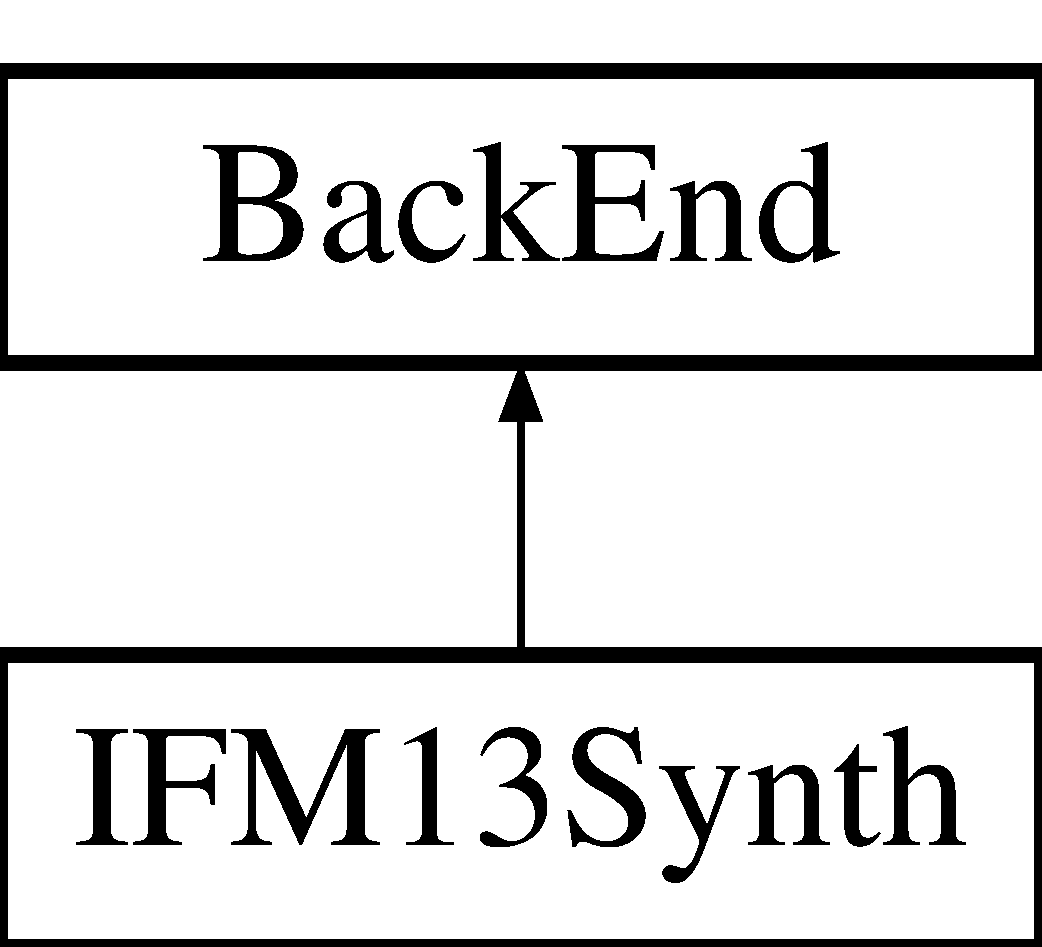
\includegraphics[height=2.000000cm]{classIFM13Synth}
\end{center}
\end{figure}
\subsection*{Public Member Functions}
\begin{DoxyCompactItemize}
\item 
\hyperlink{classIFM13Synth_ae01ff6a7fb118c2ebdc04818ef59726b}{I\-F\-M13\-Synth} (\hyperlink{classCNFImplExtractor}{C\-N\-F\-Impl\-Extractor} $\ast$impl\-\_\-extractor)
\begin{DoxyCompactList}\small\item\em Constructor. \end{DoxyCompactList}\item 
virtual \hyperlink{classIFM13Synth_ad042200b1639e702af49e55088a52f52}{$\sim$\-I\-F\-M13\-Synth} ()
\begin{DoxyCompactList}\small\item\em Destructor. \end{DoxyCompactList}\item 
virtual bool \hyperlink{classIFM13Synth_a42adb4f76d88199d92b1bedb58a139f8}{run} ()
\begin{DoxyCompactList}\small\item\em Executes the back-\/end (which is implemented as described in the I\-F\-M'13 paper). \end{DoxyCompactList}\end{DoxyCompactItemize}
\subsection*{Protected Member Functions}
\begin{DoxyCompactItemize}
\item 
bool \hyperlink{classIFM13Synth_a51c6831265e1daf7d0120c0dd954a0c4}{compute\-Winning\-Region} ()
\begin{DoxyCompactList}\small\item\em Computes the set of states from which the specification can be fulfilled. \end{DoxyCompactList}\item 
size\-\_\-t \hyperlink{classIFM13Synth_ad9262224ce1ddbda37d748fbecfe5d8e}{propagate\-Blocked\-States} (size\-\_\-t max\-\_\-level)
\begin{DoxyCompactList}\small\item\em Propagates clauses forward and searches for equivalent clause sets. \end{DoxyCompactList}\item 
bool \hyperlink{classIFM13Synth_af46e431e089225b58148ee317d523123}{rec\-Block\-Cube} (const vector$<$ int $>$ \&state\-\_\-cube, size\-\_\-t level)
\begin{DoxyCompactList}\small\item\em Analyzes the rank of the passed state. \end{DoxyCompactList}\item 
void \hyperlink{classIFM13Synth_a0aa3bd29c1621efda5abb30dd9357214}{add\-Blocked\-Transition} (const vector$<$ int $>$ \&state\-\_\-in\-\_\-cube, size\-\_\-t level)
\begin{DoxyCompactList}\small\item\em Marks a state-\/input-\/pair as blocked. \end{DoxyCompactList}\item 
void \hyperlink{classIFM13Synth_a31eb626e5ca0232d187e3471e8fed348}{add\-Blocked\-State} (const vector$<$ int $>$ \&state\-\_\-cube, size\-\_\-t level)
\begin{DoxyCompactList}\small\item\em Removes a state(-\/cube) from the frame R\mbox{[}level\mbox{]}. \end{DoxyCompactList}\item 
bool \hyperlink{classIFM13Synth_a27c2617424cad795b9af575a85e75071}{is\-Blocked} (const vector$<$ int $>$ \&state\-\_\-cube, size\-\_\-t level)
\begin{DoxyCompactList}\small\item\em Checks if a state is contained in a certain frame. \end{DoxyCompactList}\item 
void \hyperlink{classIFM13Synth_adf319a6748eda4aa29017a561752b262}{add\-Lose} (const vector$<$ int $>$ \&state\-\_\-cube)
\begin{DoxyCompactList}\small\item\em Removes a state(-\/cube) from the current over-\/approximation of the winning region. \end{DoxyCompactList}\item 
bool \hyperlink{classIFM13Synth_aca85bf07810f6c8cc3c3125895daf56f}{is\-Lose} (const vector$<$ int $>$ \&state\-\_\-cube)
\begin{DoxyCompactList}\small\item\em Checks if a state satisfies the current over-\/approximation of the winning region. \end{DoxyCompactList}\item 
void \hyperlink{classIFM13Synth_a1edccb04c096bb68a6fb2a8245f3129b}{gen\-And\-Block\-Trans} (const vector$<$ int $>$ \&state\-\_\-in\-\_\-cube, const vector$<$ int $>$ \&ctrl\-\_\-cube, size\-\_\-t level)
\begin{DoxyCompactList}\small\item\em Generalizes and excludes a blocked transition. \end{DoxyCompactList}\item 
\hyperlink{classCNF}{C\-N\-F} \& \hyperlink{classIFM13Synth_a050f0c3c5089ef6c5f793878bd60abc9}{get\-R} (size\-\_\-t index)
\begin{DoxyCompactList}\small\item\em Returns the frame R\mbox{[}index\mbox{]} in \hyperlink{classCNF}{C\-N\-F}. \end{DoxyCompactList}\item 
\hyperlink{classCNF}{C\-N\-F} \& \hyperlink{classIFM13Synth_a396e520b9db59b73a46a2315ee3123b4}{get\-U} (size\-\_\-t index)
\begin{DoxyCompactList}\small\item\em Returns the blocked transitions U\mbox{[}index\mbox{]} in \hyperlink{classCNF}{C\-N\-F}. \end{DoxyCompactList}\item 
\hyperlink{classSatSolver}{Sat\-Solver} $\ast$ \hyperlink{classIFM13Synth_ae97c0b41568cf25e163ab9b309f0dcaa}{get\-Goto\-Next\-Lower\-Solver} (size\-\_\-t index)
\begin{DoxyCompactList}\small\item\em Returns a solver with \hyperlink{classCNF}{C\-N\-F}\-: U\mbox{[}index\mbox{]} \& T \& R\mbox{[}index-\/1\mbox{]}'. \end{DoxyCompactList}\item 
\hyperlink{classSatSolver}{Sat\-Solver} $\ast$ \hyperlink{classIFM13Synth_af087a4ddf9026bb48a752c03e539d9da}{get\-Gen\-Block\-Trans\-Solver} (size\-\_\-t index)
\begin{DoxyCompactList}\small\item\em Returns a solver with \hyperlink{classCNF}{C\-N\-F}\-: T \& R\mbox{[}index-\/1\mbox{]}'. \end{DoxyCompactList}\item 
\hyperlink{classIFMProofObligation}{I\-F\-M\-Proof\-Obligation} \hyperlink{classIFM13Synth_a6bd825fad36c8cd64afbc2b17fff8b69}{pop\-Min} (list$<$ \hyperlink{classIFMProofObligation}{I\-F\-M\-Proof\-Obligation} $>$ \&queue)
\begin{DoxyCompactList}\small\item\em Takes a list of proof obligations and removes the element with lowest rank. \end{DoxyCompactList}\item 
void \hyperlink{classIFM13Synth_a986f63c9895b2999fe2ed27e38df4b84}{debug\-Print\-Rs} () const 
\begin{DoxyCompactList}\small\item\em A debugging utility to print all frames. \end{DoxyCompactList}\item 
void \hyperlink{classIFM13Synth_a3957fbd604e2a188e924f39d62c4cab4}{debug\-Check\-Invariants} (size\-\_\-t k)
\begin{DoxyCompactList}\small\item\em A debugging utility check invariants of the data structures. \end{DoxyCompactList}\end{DoxyCompactItemize}
\subsection*{Protected Attributes}
\begin{DoxyCompactItemize}
\item 
vector$<$ \hyperlink{classCNF}{C\-N\-F} $>$ \hyperlink{classIFM13Synth_a10aead75cfca1b96cdd6c17f6825a9b7}{r\-\_\-}
\begin{DoxyCompactList}\small\item\em The frames R\mbox{[}\mbox{]} of the algorithm. Each frame represents a set of states in \hyperlink{classCNF}{C\-N\-F}. \end{DoxyCompactList}\item 
vector$<$ \hyperlink{classCNF}{C\-N\-F} $>$ \hyperlink{classIFM13Synth_a493a9f0a3f2880597a89d48766706099}{u\-\_\-}
\begin{DoxyCompactList}\small\item\em The blocked transitions U\mbox{[}\mbox{]} of the algorithm. \end{DoxyCompactList}\item 
\hyperlink{classCNF}{C\-N\-F} \hyperlink{classIFM13Synth_ab6b54169dc042466704a4e6ceee4e94d}{win\-\_\-}
\begin{DoxyCompactList}\small\item\em The current over-\/approximation of the winning region W (for the protagonist). \end{DoxyCompactList}\item 
vector$<$ \hyperlink{classSatSolver}{Sat\-Solver} $\ast$ $>$ \hyperlink{classIFM13Synth_a4b964deefde7cd2cc4d81c8ea6f66976}{goto\-\_\-next\-\_\-lower\-\_\-solvers\-\_\-}
\begin{DoxyCompactList}\small\item\em The solvers storing the \hyperlink{classCNF}{C\-N\-F}\-: U\mbox{[}k\mbox{]} \& T \& R\mbox{[}k-\/1\mbox{]}'. \end{DoxyCompactList}\item 
vector$<$ \hyperlink{classSatSolver}{Sat\-Solver} $\ast$ $>$ \hyperlink{classIFM13Synth_a950a68d4f0efeca411ead2d4439aed9d}{gen\-\_\-block\-\_\-trans\-\_\-solvers\-\_\-}
\begin{DoxyCompactList}\small\item\em The solvers storing the \hyperlink{classCNF}{C\-N\-F}\-: T \& R\mbox{[}k-\/1\mbox{]}'. \end{DoxyCompactList}\item 
\hyperlink{classSatSolver}{Sat\-Solver} $\ast$ \hyperlink{classIFM13Synth_a08f52e41085966317cfc516bd52dc3b3}{goto\-\_\-win\-\_\-solver\-\_\-}
\begin{DoxyCompactList}\small\item\em A solver that stores the \hyperlink{classCNF}{C\-N\-F}\-: T \& W'. \end{DoxyCompactList}\item 
\hyperlink{classCNF}{C\-N\-F} \hyperlink{classIFM13Synth_a9b05f84db78c1ac1a2a8f74212f66c64}{winning\-\_\-region\-\_\-}
\begin{DoxyCompactList}\small\item\em The final winning region as computed by \hyperlink{classIFM13Synth_a51c6831265e1daf7d0120c0dd954a0c4}{compute\-Winning\-Region}. \end{DoxyCompactList}\item 
\hyperlink{classCNF}{C\-N\-F} \hyperlink{classIFM13Synth_a334e8e6b638c8c57da3db0c3d161231b}{neg\-\_\-winning\-\_\-region\-\_\-}
\begin{DoxyCompactList}\small\item\em The negated winning region as computed by \hyperlink{classIFM13Synth_a51c6831265e1daf7d0120c0dd954a0c4}{compute\-Winning\-Region}. \end{DoxyCompactList}\item 
vector$<$ int $>$ \hyperlink{classIFM13Synth_ac35a6617ca45b2aa1823c99ae7c984a4}{sin\-\_\-}
\begin{DoxyCompactList}\small\item\em The vector of present-\/ and next-\/state variables, and uncontrollable inputs. \end{DoxyCompactList}\item 
vector$<$ int $>$ \hyperlink{classIFM13Synth_abb5b5fc0fe0db0e7aff06d22547e00bd}{sicn\-\_\-}
\begin{DoxyCompactList}\small\item\em The vector of present-\/ and next-\/state variables, and all inputs. \end{DoxyCompactList}\item 
\hyperlink{classCNFImplExtractor}{C\-N\-F\-Impl\-Extractor} $\ast$ \hyperlink{classIFM13Synth_a1d87a79eab422a71fdc23f70d4279cbd}{impl\-\_\-extractor\-\_\-}
\begin{DoxyCompactList}\small\item\em The engine to use for circuit extraction. \end{DoxyCompactList}\end{DoxyCompactItemize}
\subsection*{Private Member Functions}
\begin{DoxyCompactItemize}
\item 
\hyperlink{classIFM13Synth_aaa3a0095cffcd56cc6f13ba80362a589}{I\-F\-M13\-Synth} (const \hyperlink{classIFM13Synth}{I\-F\-M13\-Synth} \&other)
\begin{DoxyCompactList}\small\item\em Copy constructor. \end{DoxyCompactList}\item 
\hyperlink{classIFM13Synth}{I\-F\-M13\-Synth} \& \hyperlink{classIFM13Synth_abbce31c761c00c1fca82f93dede10931}{operator=} (const \hyperlink{classIFM13Synth}{I\-F\-M13\-Synth} \&other)
\begin{DoxyCompactList}\small\item\em Assignment operator. \end{DoxyCompactList}\end{DoxyCompactItemize}


\subsection{Detailed Description}
Implements the S\-A\-T-\/based synthesis method published at I\-F\-M'13. 

This class is a re-\/implementation of the S\-A\-T-\/based synthesis method published in the paper\-: \char`\"{}\-Andreas Morgenstern, Manuel Gesell, Klaus Schneider\-: Solving Games Using
\-Incremental Induction, I\-F\-M 2013, pages 177-\/191\char`\"{}. It is based on the description given in the paper with only a few additional optimizations following the paper \char`\"{}\-Niklas Een, Alan Mishchenko, Robert K. Brayton\-: Efficient implementation of property
directed reachability, F\-M\-C\-A\-D 2011, pages 125-\/134\char`\"{}. All these optimizations are clearly marked in the source code. In order to understand the code in this class, you should read the I\-F\-M'13 paper first. After that, you will find a one-\/to-\/one correspondence between the functions described in the paper and the methods of this class.

The I\-F\-M'13 publication only describes how to determine realizability, but not how extract a winning region from this computation. Our implementation also extracts a winning region (the set R\mbox{[}i\mbox{]} such that R\mbox{[}i\mbox{]} = R\mbox{[}i-\/1\mbox{]}).

\begin{DoxyNote}{Note}
This is not the original implementation of the I\-F\-M'13 paper, it is a re-\/implementation. The re-\/implementation is based on the paper only. The original implementation may contain more optimizations. 
\end{DoxyNote}
\begin{DoxyAuthor}{Author}
Robert Koenighofer (\href{mailto:robert.koenighofer@iaik.tugraz.at}{\tt robert.\-koenighofer@iaik.\-tugraz.\-at}) 
\end{DoxyAuthor}
\begin{DoxyVersion}{Version}
1.\-1.\-0 
\end{DoxyVersion}


Definition at line 65 of file I\-F\-M13\-Synth.\-h.



\subsection{Constructor \& Destructor Documentation}
\hypertarget{classIFM13Synth_ae01ff6a7fb118c2ebdc04818ef59726b}{\index{I\-F\-M13\-Synth@{I\-F\-M13\-Synth}!I\-F\-M13\-Synth@{I\-F\-M13\-Synth}}
\index{I\-F\-M13\-Synth@{I\-F\-M13\-Synth}!IFM13Synth@{I\-F\-M13\-Synth}}
\subsubsection[{I\-F\-M13\-Synth}]{\setlength{\rightskip}{0pt plus 5cm}I\-F\-M13\-Synth\-::\-I\-F\-M13\-Synth (
\begin{DoxyParamCaption}
\item[{{\bf C\-N\-F\-Impl\-Extractor} $\ast$}]{impl\-\_\-extractor}
\end{DoxyParamCaption}
)}}\label{classIFM13Synth_ae01ff6a7fb118c2ebdc04818ef59726b}


Constructor. 


\begin{DoxyParams}{Parameters}
{\em impl\-\_\-extractor} & The engine to use for circuit extraction. It will be deleted by this class. \\
\hline
\end{DoxyParams}


Definition at line 54 of file I\-F\-M13\-Synth.\-cpp.



References C\-N\-F\-::add\-C\-N\-F(), Var\-Info\-::\-C\-T\-R\-L, gen\-\_\-block\-\_\-trans\-\_\-solvers\-\_\-, Options\-::get\-S\-A\-T\-Solver(), Var\-Manager\-::get\-Vars\-Of\-Type(), goto\-\_\-next\-\_\-lower\-\_\-solvers\-\_\-, goto\-\_\-win\-\_\-solver\-\_\-, Sat\-Solver\-::inc\-Add\-C\-N\-F(), Var\-Info\-::\-I\-N\-P\-U\-T, Var\-Manager\-::instance(), Options\-::instance(), A\-I\-G2\-C\-N\-F\-::instance(), Var\-Info\-::\-N\-E\-X\-T\-\_\-\-S\-T\-A\-T\-E, Var\-Info\-::\-P\-R\-E\-S\-\_\-\-S\-T\-A\-T\-E, r\-\_\-, sicn\-\_\-, sin\-\_\-, Sat\-Solver\-::start\-Incremental\-Session(), u\-\_\-, and win\-\_\-.

\hypertarget{classIFM13Synth_ad042200b1639e702af49e55088a52f52}{\index{I\-F\-M13\-Synth@{I\-F\-M13\-Synth}!$\sim$\-I\-F\-M13\-Synth@{$\sim$\-I\-F\-M13\-Synth}}
\index{$\sim$\-I\-F\-M13\-Synth@{$\sim$\-I\-F\-M13\-Synth}!IFM13Synth@{I\-F\-M13\-Synth}}
\subsubsection[{$\sim$\-I\-F\-M13\-Synth}]{\setlength{\rightskip}{0pt plus 5cm}I\-F\-M13\-Synth\-::$\sim$\-I\-F\-M13\-Synth (
\begin{DoxyParamCaption}
{}
\end{DoxyParamCaption}
)\hspace{0.3cm}{\ttfamily [virtual]}}}\label{classIFM13Synth_ad042200b1639e702af49e55088a52f52}


Destructor. 



Definition at line 103 of file I\-F\-M13\-Synth.\-cpp.



References gen\-\_\-block\-\_\-trans\-\_\-solvers\-\_\-, goto\-\_\-next\-\_\-lower\-\_\-solvers\-\_\-, goto\-\_\-win\-\_\-solver\-\_\-, and impl\-\_\-extractor\-\_\-.

\hypertarget{classIFM13Synth_aaa3a0095cffcd56cc6f13ba80362a589}{\index{I\-F\-M13\-Synth@{I\-F\-M13\-Synth}!I\-F\-M13\-Synth@{I\-F\-M13\-Synth}}
\index{I\-F\-M13\-Synth@{I\-F\-M13\-Synth}!IFM13Synth@{I\-F\-M13\-Synth}}
\subsubsection[{I\-F\-M13\-Synth}]{\setlength{\rightskip}{0pt plus 5cm}I\-F\-M13\-Synth\-::\-I\-F\-M13\-Synth (
\begin{DoxyParamCaption}
\item[{const {\bf I\-F\-M13\-Synth} \&}]{other}
\end{DoxyParamCaption}
)\hspace{0.3cm}{\ttfamily [private]}}}\label{classIFM13Synth_aaa3a0095cffcd56cc6f13ba80362a589}


Copy constructor. 

The copy constructor is disabled (set private) and not implemented.


\begin{DoxyParams}{Parameters}
{\em other} & The source for creating the copy. \\
\hline
\end{DoxyParams}


\subsection{Member Function Documentation}
\hypertarget{classIFM13Synth_a31eb626e5ca0232d187e3471e8fed348}{\index{I\-F\-M13\-Synth@{I\-F\-M13\-Synth}!add\-Blocked\-State@{add\-Blocked\-State}}
\index{add\-Blocked\-State@{add\-Blocked\-State}!IFM13Synth@{I\-F\-M13\-Synth}}
\subsubsection[{add\-Blocked\-State}]{\setlength{\rightskip}{0pt plus 5cm}void I\-F\-M13\-Synth\-::add\-Blocked\-State (
\begin{DoxyParamCaption}
\item[{const vector$<$ int $>$ \&}]{state\-\_\-cube, }
\item[{size\-\_\-t}]{level}
\end{DoxyParamCaption}
)\hspace{0.3cm}{\ttfamily [protected]}}}\label{classIFM13Synth_a31eb626e5ca0232d187e3471e8fed348}


Removes a state(-\/cube) from the frame R\mbox{[}level\mbox{]}. 

This method updates R\mbox{[}level\mbox{]} \-:= R\mbox{[}level\mbox{]} \& !state\-\_\-cube. state\-\_\-cube is a potentially incomplete state-\/cube. We also update the R-\/sets of all smaller levels in the same way for syntactic containment reasons (as described in the paper).


\begin{DoxyParams}{Parameters}
{\em state\-\_\-cube} & The state-\/cube that should be removed from R\mbox{[}level\mbox{]}. The cube is potentially incomplete, i.\-e., can represent a larger set of states. \\
\hline
{\em level} & The level in which the state should be blocked (i.\-e., removed form the corresponding frame R\mbox{[}level\mbox{]}). \\
\hline
\end{DoxyParams}


Definition at line 351 of file I\-F\-M13\-Synth.\-cpp.



References C\-N\-F\-::add\-Clause(), get\-Gen\-Block\-Trans\-Solver(), get\-Goto\-Next\-Lower\-Solver(), get\-R(), Sat\-Solver\-::inc\-Add\-Clause(), Sat\-Solver\-::inc\-Is\-Sat(), Var\-Manager\-::instance(), r\-\_\-, and Utils\-::swap\-Present\-To\-Next().



Referenced by rec\-Block\-Cube().

\hypertarget{classIFM13Synth_a0aa3bd29c1621efda5abb30dd9357214}{\index{I\-F\-M13\-Synth@{I\-F\-M13\-Synth}!add\-Blocked\-Transition@{add\-Blocked\-Transition}}
\index{add\-Blocked\-Transition@{add\-Blocked\-Transition}!IFM13Synth@{I\-F\-M13\-Synth}}
\subsubsection[{add\-Blocked\-Transition}]{\setlength{\rightskip}{0pt plus 5cm}void I\-F\-M13\-Synth\-::add\-Blocked\-Transition (
\begin{DoxyParamCaption}
\item[{const vector$<$ int $>$ \&}]{state\-\_\-in\-\_\-cube, }
\item[{size\-\_\-t}]{level}
\end{DoxyParamCaption}
)\hspace{0.3cm}{\ttfamily [protected]}}}\label{classIFM13Synth_a0aa3bd29c1621efda5abb30dd9357214}


Marks a state-\/input-\/pair as blocked. 

The meaning is\-: we want to store the fact that a certain state-\/input pair is not helpful for the antagonist (the party controlling the inputs i) in trying to move from R\mbox{[}level\mbox{]} to R\mbox{[}level-\/1\mbox{]}. Hence, we update U\mbox{[}level\mbox{]} \-:= U\mbox{[}level\mbox{]} \& !state\-\_\-in\-\_\-cube. We also update the U-\/sets of all smaller levels in the same way for syntactic containment reasons (as described in the paper).


\begin{DoxyParams}{Parameters}
{\em state\-\_\-in\-\_\-cube} & The state-\/input pair as a cube over present state variables and uncontrollable inputs. The cube is potentially incomplete, i.\-e., can represent a larger set of state-\/input pairs. \\
\hline
{\em level} & The level in which the transition should be blocked (i.\-e., the state-\/input pair should by marked as useless for the antagonist). \\
\hline
\end{DoxyParams}


Definition at line 336 of file I\-F\-M13\-Synth.\-cpp.



References C\-N\-F\-::add\-Clause\-And\-Simplify(), get\-Goto\-Next\-Lower\-Solver(), get\-U(), and Sat\-Solver\-::inc\-Add\-Clause().



Referenced by gen\-And\-Block\-Trans().

\hypertarget{classIFM13Synth_adf319a6748eda4aa29017a561752b262}{\index{I\-F\-M13\-Synth@{I\-F\-M13\-Synth}!add\-Lose@{add\-Lose}}
\index{add\-Lose@{add\-Lose}!IFM13Synth@{I\-F\-M13\-Synth}}
\subsubsection[{add\-Lose}]{\setlength{\rightskip}{0pt plus 5cm}void I\-F\-M13\-Synth\-::add\-Lose (
\begin{DoxyParamCaption}
\item[{const vector$<$ int $>$ \&}]{state\-\_\-cube}
\end{DoxyParamCaption}
)\hspace{0.3cm}{\ttfamily [protected]}}}\label{classIFM13Synth_adf319a6748eda4aa29017a561752b262}


Removes a state(-\/cube) from the current over-\/approximation of the winning region. 

This method updates W \-:= W \& !state\-\_\-cube. state\-\_\-cube is a potentially incomplete state-\/cube.


\begin{DoxyParams}{Parameters}
{\em state\-\_\-cube} & The state-\/cube that should be removed from the current over-\/approximation of the winning region. The cube is potentially incomplete, i.\-e., \\
\hline
\end{DoxyParams}


Definition at line 405 of file I\-F\-M13\-Synth.\-cpp.



References C\-N\-F\-::add\-Clause\-And\-Simplify(), goto\-\_\-win\-\_\-solver\-\_\-, Sat\-Solver\-::inc\-Add\-Clause(), Utils\-::swap\-Present\-To\-Next(), and win\-\_\-.



Referenced by rec\-Block\-Cube().

\hypertarget{classIFM13Synth_a51c6831265e1daf7d0120c0dd954a0c4}{\index{I\-F\-M13\-Synth@{I\-F\-M13\-Synth}!compute\-Winning\-Region@{compute\-Winning\-Region}}
\index{compute\-Winning\-Region@{compute\-Winning\-Region}!IFM13Synth@{I\-F\-M13\-Synth}}
\subsubsection[{compute\-Winning\-Region}]{\setlength{\rightskip}{0pt plus 5cm}bool I\-F\-M13\-Synth\-::compute\-Winning\-Region (
\begin{DoxyParamCaption}
{}
\end{DoxyParamCaption}
)\hspace{0.3cm}{\ttfamily [protected]}}}\label{classIFM13Synth_a51c6831265e1daf7d0120c0dd954a0c4}


Computes the set of states from which the specification can be fulfilled. 

\begin{DoxyReturn}{Returns}
True if the specification is realizable, false otherwise. 
\end{DoxyReturn}


Definition at line 145 of file I\-F\-M13\-Synth.\-cpp.



References debug\-Check\-Invariants(), get\-R(), Var\-Manager\-::get\-Vars\-Of\-Type(), Var\-Manager\-::instance(), I\-S\-\_\-\-L\-O\-S\-E, L\-\_\-\-D\-B\-G, L\-\_\-\-L\-O\-G, neg\-\_\-winning\-\_\-region\-\_\-, C\-N\-F\-::negate(), Var\-Info\-::\-P\-R\-E\-S\-\_\-\-S\-T\-A\-T\-E, propagate\-Blocked\-States(), rec\-Block\-Cube(), and winning\-\_\-region\-\_\-.



Referenced by run().

\hypertarget{classIFM13Synth_a3957fbd604e2a188e924f39d62c4cab4}{\index{I\-F\-M13\-Synth@{I\-F\-M13\-Synth}!debug\-Check\-Invariants@{debug\-Check\-Invariants}}
\index{debug\-Check\-Invariants@{debug\-Check\-Invariants}!IFM13Synth@{I\-F\-M13\-Synth}}
\subsubsection[{debug\-Check\-Invariants}]{\setlength{\rightskip}{0pt plus 5cm}void I\-F\-M13\-Synth\-::debug\-Check\-Invariants (
\begin{DoxyParamCaption}
\item[{size\-\_\-t}]{k}
\end{DoxyParamCaption}
)\hspace{0.3cm}{\ttfamily [protected]}}}\label{classIFM13Synth_a3957fbd604e2a188e924f39d62c4cab4}


A debugging utility check invariants of the data structures. 

The checks are only performed in debug-\/mode. In release-\/mode, this function does nothing.


\begin{DoxyParams}{Parameters}
{\em k} & The maximum level up until which the invariants should be checked. \\
\hline
\end{DoxyParams}


Definition at line 502 of file I\-F\-M13\-Synth.\-cpp.



References Q\-B\-F\-Solver\-::\-A, C\-N\-F\-::add\-C\-N\-F(), C\-N\-F\-::clear(), Var\-Info\-::\-C\-T\-R\-L, Q\-B\-F\-Solver\-::\-E, get\-R(), Options\-::get\-S\-A\-T\-Solver(), get\-U(), Var\-Info\-::\-I\-N\-P\-U\-T, Options\-::instance(), A\-I\-G2\-C\-N\-F\-::instance(), Dep\-Q\-B\-F\-Api\-::is\-Sat(), Sat\-Solver\-::is\-Sat(), M\-A\-S\-S\-E\-R\-T, C\-N\-F\-::negate(), Var\-Info\-::\-N\-E\-X\-T\-\_\-\-S\-T\-A\-T\-E, Var\-Info\-::\-P\-R\-E\-S\-\_\-\-S\-T\-A\-T\-E, C\-N\-F\-::swap\-Present\-To\-Next(), Var\-Info\-::\-T\-M\-P, and win\-\_\-.



Referenced by compute\-Winning\-Region().

\hypertarget{classIFM13Synth_a986f63c9895b2999fe2ed27e38df4b84}{\index{I\-F\-M13\-Synth@{I\-F\-M13\-Synth}!debug\-Print\-Rs@{debug\-Print\-Rs}}
\index{debug\-Print\-Rs@{debug\-Print\-Rs}!IFM13Synth@{I\-F\-M13\-Synth}}
\subsubsection[{debug\-Print\-Rs}]{\setlength{\rightskip}{0pt plus 5cm}void I\-F\-M13\-Synth\-::debug\-Print\-Rs (
\begin{DoxyParamCaption}
{}
\end{DoxyParamCaption}
) const\hspace{0.3cm}{\ttfamily [protected]}}}\label{classIFM13Synth_a986f63c9895b2999fe2ed27e38df4b84}


A debugging utility to print all frames. 

Do this for small examples only. 

Definition at line 492 of file I\-F\-M13\-Synth.\-cpp.



References L\-\_\-\-D\-B\-G, and r\-\_\-.

\hypertarget{classIFM13Synth_a1edccb04c096bb68a6fb2a8245f3129b}{\index{I\-F\-M13\-Synth@{I\-F\-M13\-Synth}!gen\-And\-Block\-Trans@{gen\-And\-Block\-Trans}}
\index{gen\-And\-Block\-Trans@{gen\-And\-Block\-Trans}!IFM13Synth@{I\-F\-M13\-Synth}}
\subsubsection[{gen\-And\-Block\-Trans}]{\setlength{\rightskip}{0pt plus 5cm}void I\-F\-M13\-Synth\-::gen\-And\-Block\-Trans (
\begin{DoxyParamCaption}
\item[{const vector$<$ int $>$ \&}]{state\-\_\-in\-\_\-cube, }
\item[{const vector$<$ int $>$ \&}]{ctrl\-\_\-cube, }
\item[{size\-\_\-t}]{level}
\end{DoxyParamCaption}
)\hspace{0.3cm}{\ttfamily [protected]}}}\label{classIFM13Synth_a1edccb04c096bb68a6fb2a8245f3129b}


Generalizes and excludes a blocked transition. 


\begin{DoxyParams}{Parameters}
{\em state\-\_\-in\-\_\-cube} & The state-\/input cube (the transition) that should be generalized and and blocked. \\
\hline
{\em ctrl\-\_\-cube} & The control signals that can be chosen by the protagonist in order to avoid ending up in R\mbox{[}level-\/1\mbox{]}. \\
\hline
{\em level} & The frame in which the transition should be blocked. \\
\hline
\end{DoxyParams}
\begin{DoxyReturn}{Returns}
False if state\-\_\-cube satisfies W, true otherwise. 
\end{DoxyReturn}


Definition at line 422 of file I\-F\-M13\-Synth.\-cpp.



References add\-Blocked\-Transition(), get\-Gen\-Block\-Trans\-Solver(), Sat\-Solver\-::inc\-Is\-Sat\-Model\-Or\-Core(), and M\-A\-S\-S\-E\-R\-T.



Referenced by rec\-Block\-Cube().

\hypertarget{classIFM13Synth_af087a4ddf9026bb48a752c03e539d9da}{\index{I\-F\-M13\-Synth@{I\-F\-M13\-Synth}!get\-Gen\-Block\-Trans\-Solver@{get\-Gen\-Block\-Trans\-Solver}}
\index{get\-Gen\-Block\-Trans\-Solver@{get\-Gen\-Block\-Trans\-Solver}!IFM13Synth@{I\-F\-M13\-Synth}}
\subsubsection[{get\-Gen\-Block\-Trans\-Solver}]{\setlength{\rightskip}{0pt plus 5cm}{\bf Sat\-Solver} $\ast$ I\-F\-M13\-Synth\-::get\-Gen\-Block\-Trans\-Solver (
\begin{DoxyParamCaption}
\item[{size\-\_\-t}]{index}
\end{DoxyParamCaption}
)\hspace{0.3cm}{\ttfamily [protected]}}}\label{classIFM13Synth_af087a4ddf9026bb48a752c03e539d9da}


Returns a solver with \hyperlink{classCNF}{C\-N\-F}\-: T \& R\mbox{[}index-\/1\mbox{]}'. 

This solver is used to generalize blocked transitions. If the solver for this index does not yet exists, it is created.


\begin{DoxyParams}{Parameters}
{\em index} & The index of the requested solver. \\
\hline
\end{DoxyParams}
\begin{DoxyReturn}{Returns}
A solver with \hyperlink{classCNF}{C\-N\-F}\-: T \& R\mbox{[}index-\/1\mbox{]}'. get\-Gen\-Block\-Trans\-Solver(0) returns N\-U\-L\-L. 
\end{DoxyReturn}


Definition at line 463 of file I\-F\-M13\-Synth.\-cpp.



References gen\-\_\-block\-\_\-trans\-\_\-solvers\-\_\-, Options\-::instance(), A\-I\-G2\-C\-N\-F\-::instance(), and sicn\-\_\-.



Referenced by add\-Blocked\-State(), gen\-And\-Block\-Trans(), and propagate\-Blocked\-States().

\hypertarget{classIFM13Synth_ae97c0b41568cf25e163ab9b309f0dcaa}{\index{I\-F\-M13\-Synth@{I\-F\-M13\-Synth}!get\-Goto\-Next\-Lower\-Solver@{get\-Goto\-Next\-Lower\-Solver}}
\index{get\-Goto\-Next\-Lower\-Solver@{get\-Goto\-Next\-Lower\-Solver}!IFM13Synth@{I\-F\-M13\-Synth}}
\subsubsection[{get\-Goto\-Next\-Lower\-Solver}]{\setlength{\rightskip}{0pt plus 5cm}{\bf Sat\-Solver} $\ast$ I\-F\-M13\-Synth\-::get\-Goto\-Next\-Lower\-Solver (
\begin{DoxyParamCaption}
\item[{size\-\_\-t}]{index}
\end{DoxyParamCaption}
)\hspace{0.3cm}{\ttfamily [protected]}}}\label{classIFM13Synth_ae97c0b41568cf25e163ab9b309f0dcaa}


Returns a solver with \hyperlink{classCNF}{C\-N\-F}\-: U\mbox{[}index\mbox{]} \& T \& R\mbox{[}index-\/1\mbox{]}'. 

This solver is used to search for moves the antagonist can make in order to reach R\mbox{[}index-\/1\mbox{]}. If the solver for this index does not yet exists, it is created.


\begin{DoxyParams}{Parameters}
{\em index} & The index of the requested solver. \\
\hline
\end{DoxyParams}
\begin{DoxyReturn}{Returns}
A solver with \hyperlink{classCNF}{C\-N\-F}\-: U\mbox{[}index\mbox{]} \& T \& R\mbox{[}index-\/1\mbox{]}'. get\-Goto\-Next\-Lower\-Solver(0) returns N\-U\-L\-L. 
\end{DoxyReturn}


Definition at line 451 of file I\-F\-M13\-Synth.\-cpp.



References goto\-\_\-next\-\_\-lower\-\_\-solvers\-\_\-, Options\-::instance(), A\-I\-G2\-C\-N\-F\-::instance(), and sicn\-\_\-.



Referenced by add\-Blocked\-State(), add\-Blocked\-Transition(), propagate\-Blocked\-States(), and rec\-Block\-Cube().

\hypertarget{classIFM13Synth_a050f0c3c5089ef6c5f793878bd60abc9}{\index{I\-F\-M13\-Synth@{I\-F\-M13\-Synth}!get\-R@{get\-R}}
\index{get\-R@{get\-R}!IFM13Synth@{I\-F\-M13\-Synth}}
\subsubsection[{get\-R}]{\setlength{\rightskip}{0pt plus 5cm}{\bf C\-N\-F} \& I\-F\-M13\-Synth\-::get\-R (
\begin{DoxyParamCaption}
\item[{size\-\_\-t}]{index}
\end{DoxyParamCaption}
)\hspace{0.3cm}{\ttfamily [protected]}}}\label{classIFM13Synth_a050f0c3c5089ef6c5f793878bd60abc9}


Returns the frame R\mbox{[}index\mbox{]} in \hyperlink{classCNF}{C\-N\-F}. 

If the frame with this index does not yet exists, it is created.


\begin{DoxyParams}{Parameters}
{\em index} & The index of the requested frame. \\
\hline
\end{DoxyParams}
\begin{DoxyReturn}{Returns}
The frame R\mbox{[}index\mbox{]} in \hyperlink{classCNF}{C\-N\-F}. 
\end{DoxyReturn}


Definition at line 435 of file I\-F\-M13\-Synth.\-cpp.



References r\-\_\-.



Referenced by add\-Blocked\-State(), compute\-Winning\-Region(), debug\-Check\-Invariants(), is\-Blocked(), and propagate\-Blocked\-States().

\hypertarget{classIFM13Synth_a396e520b9db59b73a46a2315ee3123b4}{\index{I\-F\-M13\-Synth@{I\-F\-M13\-Synth}!get\-U@{get\-U}}
\index{get\-U@{get\-U}!IFM13Synth@{I\-F\-M13\-Synth}}
\subsubsection[{get\-U}]{\setlength{\rightskip}{0pt plus 5cm}{\bf C\-N\-F} \& I\-F\-M13\-Synth\-::get\-U (
\begin{DoxyParamCaption}
\item[{size\-\_\-t}]{index}
\end{DoxyParamCaption}
)\hspace{0.3cm}{\ttfamily [protected]}}}\label{classIFM13Synth_a396e520b9db59b73a46a2315ee3123b4}


Returns the blocked transitions U\mbox{[}index\mbox{]} in \hyperlink{classCNF}{C\-N\-F}. 

If the set of blocked transitions with this index does not yet exists, it is created. This function is actually only needed for debugging purposes.


\begin{DoxyParams}{Parameters}
{\em index} & The index of the requested set of blocked transitions. \\
\hline
\end{DoxyParams}
\begin{DoxyReturn}{Returns}
The set U\mbox{[}index\mbox{]} of blocked transitions in \hyperlink{classCNF}{C\-N\-F}. 
\end{DoxyReturn}


Definition at line 443 of file I\-F\-M13\-Synth.\-cpp.



References u\-\_\-.



Referenced by add\-Blocked\-Transition(), and debug\-Check\-Invariants().

\hypertarget{classIFM13Synth_a27c2617424cad795b9af575a85e75071}{\index{I\-F\-M13\-Synth@{I\-F\-M13\-Synth}!is\-Blocked@{is\-Blocked}}
\index{is\-Blocked@{is\-Blocked}!IFM13Synth@{I\-F\-M13\-Synth}}
\subsubsection[{is\-Blocked}]{\setlength{\rightskip}{0pt plus 5cm}bool I\-F\-M13\-Synth\-::is\-Blocked (
\begin{DoxyParamCaption}
\item[{const vector$<$ int $>$ \&}]{state\-\_\-cube, }
\item[{size\-\_\-t}]{level}
\end{DoxyParamCaption}
)\hspace{0.3cm}{\ttfamily [protected]}}}\label{classIFM13Synth_a27c2617424cad795b9af575a85e75071}


Checks if a state is contained in a certain frame. 

The passed state cube is complete, i.\-e., contains all state variables. Hence, containment can be (and is) checked syntactically. We simply check if state\-\_\-cube satisfies all clauses of R\mbox{[}level\mbox{]}.


\begin{DoxyParams}{Parameters}
{\em state\-\_\-cube} & A full cube over the present state variables. \\
\hline
{\em level} & The index i of a certain frame R\mbox{[}i\mbox{]}. \\
\hline
\end{DoxyParams}
\begin{DoxyReturn}{Returns}
False if state\-\_\-cube satisfies R\mbox{[}level\mbox{]}, true otherwise. 
\end{DoxyReturn}


Definition at line 399 of file I\-F\-M13\-Synth.\-cpp.



References get\-R(), and C\-N\-F\-::is\-Sat\-By().



Referenced by rec\-Block\-Cube().

\hypertarget{classIFM13Synth_aca85bf07810f6c8cc3c3125895daf56f}{\index{I\-F\-M13\-Synth@{I\-F\-M13\-Synth}!is\-Lose@{is\-Lose}}
\index{is\-Lose@{is\-Lose}!IFM13Synth@{I\-F\-M13\-Synth}}
\subsubsection[{is\-Lose}]{\setlength{\rightskip}{0pt plus 5cm}bool I\-F\-M13\-Synth\-::is\-Lose (
\begin{DoxyParamCaption}
\item[{const vector$<$ int $>$ \&}]{state\-\_\-cube}
\end{DoxyParamCaption}
)\hspace{0.3cm}{\ttfamily [protected]}}}\label{classIFM13Synth_aca85bf07810f6c8cc3c3125895daf56f}


Checks if a state satisfies the current over-\/approximation of the winning region. 

The passed state cube is complete, i.\-e., contains all state variables. Hence, containment can be (and is) checked syntactically. We simply check if state\-\_\-cube satisfies all clauses of W (stored in \hyperlink{classIFM13Synth_ab6b54169dc042466704a4e6ceee4e94d}{win\-\_\- }).


\begin{DoxyParams}{Parameters}
{\em state\-\_\-cube} & A full cube over the present state variables. \\
\hline
\end{DoxyParams}
\begin{DoxyReturn}{Returns}
False if state\-\_\-cube satisfies W, true otherwise. 
\end{DoxyReturn}


Definition at line 416 of file I\-F\-M13\-Synth.\-cpp.



References C\-N\-F\-::is\-Sat\-By(), and win\-\_\-.



Referenced by rec\-Block\-Cube().

\hypertarget{classIFM13Synth_abbce31c761c00c1fca82f93dede10931}{\index{I\-F\-M13\-Synth@{I\-F\-M13\-Synth}!operator=@{operator=}}
\index{operator=@{operator=}!IFM13Synth@{I\-F\-M13\-Synth}}
\subsubsection[{operator=}]{\setlength{\rightskip}{0pt plus 5cm}{\bf I\-F\-M13\-Synth}\& I\-F\-M13\-Synth\-::operator= (
\begin{DoxyParamCaption}
\item[{const {\bf I\-F\-M13\-Synth} \&}]{other}
\end{DoxyParamCaption}
)\hspace{0.3cm}{\ttfamily [private]}}}\label{classIFM13Synth_abbce31c761c00c1fca82f93dede10931}


Assignment operator. 

The assignment operator is disabled (set private) and not implemented.


\begin{DoxyParams}{Parameters}
{\em other} & The source for creating the copy. \\
\hline
\end{DoxyParams}
\begin{DoxyReturn}{Returns}
The result of the assignment, i.\-e, $\ast$this. 
\end{DoxyReturn}
\hypertarget{classIFM13Synth_a6bd825fad36c8cd64afbc2b17fff8b69}{\index{I\-F\-M13\-Synth@{I\-F\-M13\-Synth}!pop\-Min@{pop\-Min}}
\index{pop\-Min@{pop\-Min}!IFM13Synth@{I\-F\-M13\-Synth}}
\subsubsection[{pop\-Min}]{\setlength{\rightskip}{0pt plus 5cm}{\bf I\-F\-M\-Proof\-Obligation} I\-F\-M13\-Synth\-::pop\-Min (
\begin{DoxyParamCaption}
\item[{list$<$ {\bf I\-F\-M\-Proof\-Obligation} $>$ \&}]{queue}
\end{DoxyParamCaption}
)\hspace{0.3cm}{\ttfamily [protected]}}}\label{classIFM13Synth_a6bd825fad36c8cd64afbc2b17fff8b69}


Takes a list of proof obligations and removes the element with lowest rank. 


\begin{DoxyParams}{Parameters}
{\em queue} & A list of proof obligations. \\
\hline
\end{DoxyParams}
\begin{DoxyReturn}{Returns}
The element that has been removed from the list. It is always the element (among the elements) with minimal rank. 
\end{DoxyReturn}


Definition at line 475 of file I\-F\-M13\-Synth.\-cpp.



References M\-A\-S\-S\-E\-R\-T.



Referenced by rec\-Block\-Cube().

\hypertarget{classIFM13Synth_ad9262224ce1ddbda37d748fbecfe5d8e}{\index{I\-F\-M13\-Synth@{I\-F\-M13\-Synth}!propagate\-Blocked\-States@{propagate\-Blocked\-States}}
\index{propagate\-Blocked\-States@{propagate\-Blocked\-States}!IFM13Synth@{I\-F\-M13\-Synth}}
\subsubsection[{propagate\-Blocked\-States}]{\setlength{\rightskip}{0pt plus 5cm}size\-\_\-t I\-F\-M13\-Synth\-::propagate\-Blocked\-States (
\begin{DoxyParamCaption}
\item[{size\-\_\-t}]{max\-\_\-level}
\end{DoxyParamCaption}
)\hspace{0.3cm}{\ttfamily [protected]}}}\label{classIFM13Synth_ad9262224ce1ddbda37d748fbecfe5d8e}


Propagates clauses forward and searches for equivalent clause sets. 

Similar to I\-C3, this method propagates clauses of frames forward. It also checks if two adjacent clauses sets become syntactically equal.


\begin{DoxyParams}{Parameters}
{\em max\-\_\-level} & The maximum frame level until which propagation should be performed. \\
\hline
\end{DoxyParams}
\begin{DoxyReturn}{Returns}
The number N returned by this method has the following meaning\-: N=0 means that no equal clause sets have been found. N $>$ 0 means that R\mbox{[}N\mbox{]} = R\mbox{[}N-\/1\mbox{]}. 
\end{DoxyReturn}


Definition at line 177 of file I\-F\-M13\-Synth.\-cpp.



References C\-N\-F\-::get\-Clauses(), get\-Gen\-Block\-Trans\-Solver(), get\-Goto\-Next\-Lower\-Solver(), get\-R(), Sat\-Solver\-::inc\-Add\-Clause(), Sat\-Solver\-::inc\-Is\-Sat(), C\-N\-F\-::remove\-Duplicates(), Utils\-::swap\-Present\-To\-Next(), and C\-N\-F\-::swap\-With().



Referenced by compute\-Winning\-Region().

\hypertarget{classIFM13Synth_af46e431e089225b58148ee317d523123}{\index{I\-F\-M13\-Synth@{I\-F\-M13\-Synth}!rec\-Block\-Cube@{rec\-Block\-Cube}}
\index{rec\-Block\-Cube@{rec\-Block\-Cube}!IFM13Synth@{I\-F\-M13\-Synth}}
\subsubsection[{rec\-Block\-Cube}]{\setlength{\rightskip}{0pt plus 5cm}bool I\-F\-M13\-Synth\-::rec\-Block\-Cube (
\begin{DoxyParamCaption}
\item[{const vector$<$ int $>$ \&}]{state\-\_\-cube, }
\item[{size\-\_\-t}]{level}
\end{DoxyParamCaption}
)\hspace{0.3cm}{\ttfamily [protected]}}}\label{classIFM13Synth_af46e431e089225b58148ee317d523123}


Analyzes the rank of the passed state. 

There are two possible conclusions\-: (a) the rank of the state is $>$ level, (b) the rank of the state is $<$= level. In order to analyze a certain state, this method may analyze some of its successor states first (using a queue of proof obligations internally). This method is always called for the initial state only.


\begin{DoxyParams}{Parameters}
{\em state\-\_\-cube} & A full cube over the state variables, describing the state that should be analyzed. \\
\hline
{\em level} & The level for the analysis (this method checks if the rank of the state is $>$ level or $<$= level). \\
\hline
\end{DoxyParams}
\begin{DoxyReturn}{Returns}
I\-S\-\_\-\-G\-R\-E\-A\-T\-E\-R (an alias for true) if the rank of the state is $>$ level. I\-S\-\_\-\-L\-O\-S\-E (an alias for false) otherwise. 
\end{DoxyReturn}


Definition at line 229 of file I\-F\-M13\-Synth.\-cpp.



References add\-Blocked\-State(), add\-Lose(), Utils\-::contains\-Init(), Var\-Info\-::\-C\-T\-R\-L, Utils\-::extract(), Utils\-::extract\-Next\-As\-Present(), Utils\-::extract\-Pres\-In(), gen\-And\-Block\-Trans(), get\-Goto\-Next\-Lower\-Solver(), I\-F\-M\-Proof\-Obligation\-::get\-Level(), I\-F\-M\-Proof\-Obligation\-::get\-Pre\-Ctrl\-Cube(), I\-F\-M\-Proof\-Obligation\-::get\-Pre\-State\-In\-Cube(), I\-F\-M\-Proof\-Obligation\-::get\-State(), goto\-\_\-win\-\_\-solver\-\_\-, I\-F\-M\-Proof\-Obligation\-::has\-Pre(), Sat\-Solver\-::inc\-Is\-Sat\-Model\-Or\-Core(), Var\-Info\-::\-I\-N\-P\-U\-T, I\-S\-\_\-\-G\-R\-E\-A\-T\-E\-R, I\-S\-\_\-\-L\-O\-S\-E, is\-Blocked(), is\-Lose(), pop\-Min(), Var\-Info\-::\-P\-R\-E\-S\-\_\-\-S\-T\-A\-T\-E, sicn\-\_\-, and sin\-\_\-.



Referenced by compute\-Winning\-Region().

\hypertarget{classIFM13Synth_a42adb4f76d88199d92b1bedb58a139f8}{\index{I\-F\-M13\-Synth@{I\-F\-M13\-Synth}!run@{run}}
\index{run@{run}!IFM13Synth@{I\-F\-M13\-Synth}}
\subsubsection[{run}]{\setlength{\rightskip}{0pt plus 5cm}bool I\-F\-M13\-Synth\-::run (
\begin{DoxyParamCaption}
{}
\end{DoxyParamCaption}
)\hspace{0.3cm}{\ttfamily [virtual]}}}\label{classIFM13Synth_a42adb4f76d88199d92b1bedb58a139f8}


Executes the back-\/end (which is implemented as described in the I\-F\-M'13 paper). 

This method is the workhorse of this class. It implements the S\-A\-T-\/based synthesis method published in the paper\-: \char`\"{}\-Andreas Morgenstern, Manuel Gesell, Klaus Schneider\-: Solving
\-Games Using Incremental Induction, I\-F\-M 2013, pages 177-\/191\char`\"{}. It is based on the description given in the paper with only a few additional optimizations following the paper \char`\"{}\-Niklas Een, Alan Mishchenko, Robert K. Brayton\-: Efficient implementation of
property directed reachability, F\-M\-C\-A\-D 2011, pages 125-\/134\char`\"{}. All these optimizations are clearly marked in the source code. In order to understand the code in this class, you should read the I\-F\-M'13 paper first. After that, you will find a one-\/to-\/one correspondence between the functions described in the paper and the methods of this class.

The I\-F\-M'13 publication only describes how to determine realizability, but not how extract a winning region from this computation. Our implementation also extracts a winning region (the set R\mbox{[}i\mbox{]} such that R\mbox{[}i\mbox{]} = R\mbox{[}i-\/1\mbox{]}).

\begin{DoxyReturn}{Returns}
True if the specification was realizable, false otherwise. 
\end{DoxyReturn}


Implements \hyperlink{classBackEnd_a099e717dc71e9cc2d838b1ca86340590}{Back\-End}.



Definition at line 121 of file I\-F\-M13\-Synth.\-cpp.



References compute\-Winning\-Region(), Utils\-::debug\-Check\-Win\-Reg(), C\-N\-F\-Impl\-Extractor\-::extract\-Circuit(), impl\-\_\-extractor\-\_\-, Options\-::instance(), L\-\_\-\-I\-N\-F, L\-\_\-\-R\-E\-S, C\-N\-F\-Impl\-Extractor\-::log\-Statistics(), neg\-\_\-winning\-\_\-region\-\_\-, and winning\-\_\-region\-\_\-.



\subsection{Member Data Documentation}
\hypertarget{classIFM13Synth_a950a68d4f0efeca411ead2d4439aed9d}{\index{I\-F\-M13\-Synth@{I\-F\-M13\-Synth}!gen\-\_\-block\-\_\-trans\-\_\-solvers\-\_\-@{gen\-\_\-block\-\_\-trans\-\_\-solvers\-\_\-}}
\index{gen\-\_\-block\-\_\-trans\-\_\-solvers\-\_\-@{gen\-\_\-block\-\_\-trans\-\_\-solvers\-\_\-}!IFM13Synth@{I\-F\-M13\-Synth}}
\subsubsection[{gen\-\_\-block\-\_\-trans\-\_\-solvers\-\_\-}]{\setlength{\rightskip}{0pt plus 5cm}vector$<${\bf Sat\-Solver}$\ast$$>$ I\-F\-M13\-Synth\-::gen\-\_\-block\-\_\-trans\-\_\-solvers\-\_\-\hspace{0.3cm}{\ttfamily [protected]}}}\label{classIFM13Synth_a950a68d4f0efeca411ead2d4439aed9d}


The solvers storing the \hyperlink{classCNF}{C\-N\-F}\-: T \& R\mbox{[}k-\/1\mbox{]}'. 

You should use \hyperlink{classIFM13Synth_af087a4ddf9026bb48a752c03e539d9da}{get\-Gen\-Block\-Trans\-Solver() } to access these solvers. The reason is that this method initializes the solvers if they do not yet exist. gen\-\_\-block\-\_\-trans\-\_\-solvers\-\_\-\mbox{[}0\mbox{]} is always N\-U\-L\-L. 

Definition at line 333 of file I\-F\-M13\-Synth.\-h.



Referenced by get\-Gen\-Block\-Trans\-Solver(), I\-F\-M13\-Synth(), and $\sim$\-I\-F\-M13\-Synth().

\hypertarget{classIFM13Synth_a4b964deefde7cd2cc4d81c8ea6f66976}{\index{I\-F\-M13\-Synth@{I\-F\-M13\-Synth}!goto\-\_\-next\-\_\-lower\-\_\-solvers\-\_\-@{goto\-\_\-next\-\_\-lower\-\_\-solvers\-\_\-}}
\index{goto\-\_\-next\-\_\-lower\-\_\-solvers\-\_\-@{goto\-\_\-next\-\_\-lower\-\_\-solvers\-\_\-}!IFM13Synth@{I\-F\-M13\-Synth}}
\subsubsection[{goto\-\_\-next\-\_\-lower\-\_\-solvers\-\_\-}]{\setlength{\rightskip}{0pt plus 5cm}vector$<${\bf Sat\-Solver}$\ast$$>$ I\-F\-M13\-Synth\-::goto\-\_\-next\-\_\-lower\-\_\-solvers\-\_\-\hspace{0.3cm}{\ttfamily [protected]}}}\label{classIFM13Synth_a4b964deefde7cd2cc4d81c8ea6f66976}


The solvers storing the \hyperlink{classCNF}{C\-N\-F}\-: U\mbox{[}k\mbox{]} \& T \& R\mbox{[}k-\/1\mbox{]}'. 

These solvers are used to search for moves the antagonist can make in order to reach R\mbox{[}k-\/1\mbox{]}. You should use \hyperlink{classIFM13Synth_ae97c0b41568cf25e163ab9b309f0dcaa}{get\-Goto\-Next\-Lower\-Solver() } to access these solvers. The reason is that this method initializes the solvers if they do not yet exist. goto\-\_\-next\-\_\-lower\-\_\-solvers\-\_\-\mbox{[}0\mbox{]} is always N\-U\-L\-L. 

Definition at line 324 of file I\-F\-M13\-Synth.\-h.



Referenced by get\-Goto\-Next\-Lower\-Solver(), I\-F\-M13\-Synth(), and $\sim$\-I\-F\-M13\-Synth().

\hypertarget{classIFM13Synth_a08f52e41085966317cfc516bd52dc3b3}{\index{I\-F\-M13\-Synth@{I\-F\-M13\-Synth}!goto\-\_\-win\-\_\-solver\-\_\-@{goto\-\_\-win\-\_\-solver\-\_\-}}
\index{goto\-\_\-win\-\_\-solver\-\_\-@{goto\-\_\-win\-\_\-solver\-\_\-}!IFM13Synth@{I\-F\-M13\-Synth}}
\subsubsection[{goto\-\_\-win\-\_\-solver\-\_\-}]{\setlength{\rightskip}{0pt plus 5cm}{\bf Sat\-Solver}$\ast$ I\-F\-M13\-Synth\-::goto\-\_\-win\-\_\-solver\-\_\-\hspace{0.3cm}{\ttfamily [protected]}}}\label{classIFM13Synth_a08f52e41085966317cfc516bd52dc3b3}


A solver that stores the \hyperlink{classCNF}{C\-N\-F}\-: T \& W'. 



Definition at line 338 of file I\-F\-M13\-Synth.\-h.



Referenced by add\-Lose(), I\-F\-M13\-Synth(), rec\-Block\-Cube(), and $\sim$\-I\-F\-M13\-Synth().

\hypertarget{classIFM13Synth_a1d87a79eab422a71fdc23f70d4279cbd}{\index{I\-F\-M13\-Synth@{I\-F\-M13\-Synth}!impl\-\_\-extractor\-\_\-@{impl\-\_\-extractor\-\_\-}}
\index{impl\-\_\-extractor\-\_\-@{impl\-\_\-extractor\-\_\-}!IFM13Synth@{I\-F\-M13\-Synth}}
\subsubsection[{impl\-\_\-extractor\-\_\-}]{\setlength{\rightskip}{0pt plus 5cm}{\bf C\-N\-F\-Impl\-Extractor}$\ast$ I\-F\-M13\-Synth\-::impl\-\_\-extractor\-\_\-\hspace{0.3cm}{\ttfamily [protected]}}}\label{classIFM13Synth_a1d87a79eab422a71fdc23f70d4279cbd}


The engine to use for circuit extraction. 

It will be deleted by this class (in the destructor). 

Definition at line 365 of file I\-F\-M13\-Synth.\-h.



Referenced by run(), and $\sim$\-I\-F\-M13\-Synth().

\hypertarget{classIFM13Synth_a334e8e6b638c8c57da3db0c3d161231b}{\index{I\-F\-M13\-Synth@{I\-F\-M13\-Synth}!neg\-\_\-winning\-\_\-region\-\_\-@{neg\-\_\-winning\-\_\-region\-\_\-}}
\index{neg\-\_\-winning\-\_\-region\-\_\-@{neg\-\_\-winning\-\_\-region\-\_\-}!IFM13Synth@{I\-F\-M13\-Synth}}
\subsubsection[{neg\-\_\-winning\-\_\-region\-\_\-}]{\setlength{\rightskip}{0pt plus 5cm}{\bf C\-N\-F} I\-F\-M13\-Synth\-::neg\-\_\-winning\-\_\-region\-\_\-\hspace{0.3cm}{\ttfamily [protected]}}}\label{classIFM13Synth_a334e8e6b638c8c57da3db0c3d161231b}


The negated winning region as computed by \hyperlink{classIFM13Synth_a51c6831265e1daf7d0120c0dd954a0c4}{compute\-Winning\-Region}. 



Definition at line 348 of file I\-F\-M13\-Synth.\-h.



Referenced by compute\-Winning\-Region(), and run().

\hypertarget{classIFM13Synth_a10aead75cfca1b96cdd6c17f6825a9b7}{\index{I\-F\-M13\-Synth@{I\-F\-M13\-Synth}!r\-\_\-@{r\-\_\-}}
\index{r\-\_\-@{r\-\_\-}!IFM13Synth@{I\-F\-M13\-Synth}}
\subsubsection[{r\-\_\-}]{\setlength{\rightskip}{0pt plus 5cm}vector$<${\bf C\-N\-F}$>$ I\-F\-M13\-Synth\-::r\-\_\-\hspace{0.3cm}{\ttfamily [protected]}}}\label{classIFM13Synth_a10aead75cfca1b96cdd6c17f6825a9b7}


The frames R\mbox{[}\mbox{]} of the algorithm. Each frame represents a set of states in \hyperlink{classCNF}{C\-N\-F}. 

You should use \hyperlink{classIFM13Synth_a050f0c3c5089ef6c5f793878bd60abc9}{get\-R() } to access the frames. The reason is that this method initializes frames if they do not yet exist. 

Definition at line 298 of file I\-F\-M13\-Synth.\-h.



Referenced by add\-Blocked\-State(), debug\-Print\-Rs(), get\-R(), and I\-F\-M13\-Synth().

\hypertarget{classIFM13Synth_abb5b5fc0fe0db0e7aff06d22547e00bd}{\index{I\-F\-M13\-Synth@{I\-F\-M13\-Synth}!sicn\-\_\-@{sicn\-\_\-}}
\index{sicn\-\_\-@{sicn\-\_\-}!IFM13Synth@{I\-F\-M13\-Synth}}
\subsubsection[{sicn\-\_\-}]{\setlength{\rightskip}{0pt plus 5cm}vector$<$int$>$ I\-F\-M13\-Synth\-::sicn\-\_\-\hspace{0.3cm}{\ttfamily [protected]}}}\label{classIFM13Synth_abb5b5fc0fe0db0e7aff06d22547e00bd}


The vector of present-\/ and next-\/state variables, and all inputs. 



Definition at line 358 of file I\-F\-M13\-Synth.\-h.



Referenced by get\-Gen\-Block\-Trans\-Solver(), get\-Goto\-Next\-Lower\-Solver(), I\-F\-M13\-Synth(), and rec\-Block\-Cube().

\hypertarget{classIFM13Synth_ac35a6617ca45b2aa1823c99ae7c984a4}{\index{I\-F\-M13\-Synth@{I\-F\-M13\-Synth}!sin\-\_\-@{sin\-\_\-}}
\index{sin\-\_\-@{sin\-\_\-}!IFM13Synth@{I\-F\-M13\-Synth}}
\subsubsection[{sin\-\_\-}]{\setlength{\rightskip}{0pt plus 5cm}vector$<$int$>$ I\-F\-M13\-Synth\-::sin\-\_\-\hspace{0.3cm}{\ttfamily [protected]}}}\label{classIFM13Synth_ac35a6617ca45b2aa1823c99ae7c984a4}


The vector of present-\/ and next-\/state variables, and uncontrollable inputs. 



Definition at line 353 of file I\-F\-M13\-Synth.\-h.



Referenced by I\-F\-M13\-Synth(), and rec\-Block\-Cube().

\hypertarget{classIFM13Synth_a493a9f0a3f2880597a89d48766706099}{\index{I\-F\-M13\-Synth@{I\-F\-M13\-Synth}!u\-\_\-@{u\-\_\-}}
\index{u\-\_\-@{u\-\_\-}!IFM13Synth@{I\-F\-M13\-Synth}}
\subsubsection[{u\-\_\-}]{\setlength{\rightskip}{0pt plus 5cm}vector$<${\bf C\-N\-F}$>$ I\-F\-M13\-Synth\-::u\-\_\-\hspace{0.3cm}{\ttfamily [protected]}}}\label{classIFM13Synth_a493a9f0a3f2880597a89d48766706099}


The blocked transitions U\mbox{[}\mbox{]} of the algorithm. 

These sets are maintained only in debug mode. In release-\/mode they are only present inside the goto\-\_\-next\-\_\-lower\-\_\-solvers\-\_\-. You should use \hyperlink{classIFM13Synth_a396e520b9db59b73a46a2315ee3123b4}{get\-U() } to access the frames. The reason is that this method initializes elements if they do not yet exist. 

Definition at line 308 of file I\-F\-M13\-Synth.\-h.



Referenced by get\-U(), and I\-F\-M13\-Synth().

\hypertarget{classIFM13Synth_ab6b54169dc042466704a4e6ceee4e94d}{\index{I\-F\-M13\-Synth@{I\-F\-M13\-Synth}!win\-\_\-@{win\-\_\-}}
\index{win\-\_\-@{win\-\_\-}!IFM13Synth@{I\-F\-M13\-Synth}}
\subsubsection[{win\-\_\-}]{\setlength{\rightskip}{0pt plus 5cm}{\bf C\-N\-F} I\-F\-M13\-Synth\-::win\-\_\-\hspace{0.3cm}{\ttfamily [protected]}}}\label{classIFM13Synth_ab6b54169dc042466704a4e6ceee4e94d}


The current over-\/approximation of the winning region W (for the protagonist). 



Definition at line 313 of file I\-F\-M13\-Synth.\-h.



Referenced by add\-Lose(), debug\-Check\-Invariants(), I\-F\-M13\-Synth(), and is\-Lose().

\hypertarget{classIFM13Synth_a9b05f84db78c1ac1a2a8f74212f66c64}{\index{I\-F\-M13\-Synth@{I\-F\-M13\-Synth}!winning\-\_\-region\-\_\-@{winning\-\_\-region\-\_\-}}
\index{winning\-\_\-region\-\_\-@{winning\-\_\-region\-\_\-}!IFM13Synth@{I\-F\-M13\-Synth}}
\subsubsection[{winning\-\_\-region\-\_\-}]{\setlength{\rightskip}{0pt plus 5cm}{\bf C\-N\-F} I\-F\-M13\-Synth\-::winning\-\_\-region\-\_\-\hspace{0.3cm}{\ttfamily [protected]}}}\label{classIFM13Synth_a9b05f84db78c1ac1a2a8f74212f66c64}


The final winning region as computed by \hyperlink{classIFM13Synth_a51c6831265e1daf7d0120c0dd954a0c4}{compute\-Winning\-Region}. 



Definition at line 343 of file I\-F\-M13\-Synth.\-h.



Referenced by compute\-Winning\-Region(), and run().



The documentation for this class was generated from the following files\-:\begin{DoxyCompactItemize}
\item 
src/\hyperlink{IFM13Synth_8h}{I\-F\-M13\-Synth.\-h}\item 
src/\hyperlink{IFM13Synth_8cpp}{I\-F\-M13\-Synth.\-cpp}\end{DoxyCompactItemize}

\hypertarget{classIFMProofObligation}{\section{I\-F\-M\-Proof\-Obligation Class Reference}
\label{classIFMProofObligation}\index{I\-F\-M\-Proof\-Obligation@{I\-F\-M\-Proof\-Obligation}}
}


A helper-\/class for \hyperlink{classIFM13Synth}{I\-F\-M13\-Synth}, representing an open proof obligation.  




{\ttfamily \#include $<$I\-F\-M\-Proof\-Obligation.\-h$>$}

\subsection*{Public Member Functions}
\begin{DoxyCompactItemize}
\item 
\hyperlink{classIFMProofObligation_a5c774e39decb6399858b22192ce91ccb}{I\-F\-M\-Proof\-Obligation} (const vector$<$ int $>$ \&state\-\_\-cube, size\-\_\-t state\-\_\-level)
\begin{DoxyCompactList}\small\item\em Constructor omitting the predecessor. \end{DoxyCompactList}\item 
\hyperlink{classIFMProofObligation_ae1a80b72265ebee8fe33461119bf2ab1}{I\-F\-M\-Proof\-Obligation} (const vector$<$ int $>$ \&state\-\_\-cube, size\-\_\-t state\-\_\-level, const vector$<$ int $>$ \&pre\-\_\-state\-\_\-in\-\_\-cube, const vector$<$ int $>$ \&pre\-\_\-ctrl\-\_\-cube)
\begin{DoxyCompactList}\small\item\em Constructor also setting a predecessor. \end{DoxyCompactList}\item 
\hyperlink{classIFMProofObligation_a4f7d62a51ba4dfa4398b415034a320c6}{I\-F\-M\-Proof\-Obligation} (const \hyperlink{classIFMProofObligation}{I\-F\-M\-Proof\-Obligation} \&other)
\begin{DoxyCompactList}\small\item\em Copy constructor. \end{DoxyCompactList}\item 
\hyperlink{classIFMProofObligation}{I\-F\-M\-Proof\-Obligation} \& \hyperlink{classIFMProofObligation_ab314748b1ee6226ca48ef7a69bedff6e}{operator=} (const \hyperlink{classIFMProofObligation}{I\-F\-M\-Proof\-Obligation} \&other)
\begin{DoxyCompactList}\small\item\em Assignment operator. \end{DoxyCompactList}\item 
virtual \hyperlink{classIFMProofObligation_afcb88686953a327b0340fbf51cae2f1c}{$\sim$\-I\-F\-M\-Proof\-Obligation} ()
\begin{DoxyCompactList}\small\item\em Destructor. \end{DoxyCompactList}\item 
const vector$<$ int $>$ \& \hyperlink{classIFMProofObligation_a75083a8658b5dbc8b7d824081876170e}{get\-State} () const 
\begin{DoxyCompactList}\small\item\em Returns the state in question in form of a full cube over the state variables. \end{DoxyCompactList}\item 
size\-\_\-t \hyperlink{classIFMProofObligation_acf55ebc5c8e1720d770c99e76fb02ec5}{get\-Level} () const 
\begin{DoxyCompactList}\small\item\em Returns the level in question. \end{DoxyCompactList}\item 
bool \hyperlink{classIFMProofObligation_ad8175e23cff3378d2feb7c5bae2c171f}{has\-Pre} () const 
\begin{DoxyCompactList}\small\item\em Checks if a preprocessor was set. \end{DoxyCompactList}\item 
const vector$<$ int $>$ \& \hyperlink{classIFMProofObligation_ab9c20d91b552ef862c37837b9d707895}{get\-Pre\-State\-In\-Cube} () const 
\begin{DoxyCompactList}\small\item\em Returns the predecessor together with the inputs of the transition. \end{DoxyCompactList}\item 
const vector$<$ int $>$ \& \hyperlink{classIFMProofObligation_a577815e5d3e6205c0c3b09934489100e}{get\-Pre\-Ctrl\-Cube} () const 
\begin{DoxyCompactList}\small\item\em Returns the control values of the transition from the predecessor to the state. \end{DoxyCompactList}\item 
void \hyperlink{classIFMProofObligation_a3bca5075c133d0717af164407c2403ae}{set\-Pre} (const vector$<$ int $>$ \&pre\-\_\-state\-\_\-in\-\_\-cube, const vector$<$ int $>$ \&pre\-\_\-ctrl\-\_\-cube)
\begin{DoxyCompactList}\small\item\em Sets the predecessor and the transition to the current state. \end{DoxyCompactList}\end{DoxyCompactItemize}
\subsection*{Protected Attributes}
\begin{DoxyCompactItemize}
\item 
vector$<$ int $>$ \hyperlink{classIFMProofObligation_a688b714ebad4010c14e11355a73faf3c}{state\-\_\-cube\-\_\-}
\begin{DoxyCompactList}\small\item\em A full cube over the state-\/variables. It represents the state in question. \end{DoxyCompactList}\item 
size\-\_\-t \hyperlink{classIFMProofObligation_a6207c16b84a41450a8ca31ed8a35b4ea}{state\-\_\-level\-\_\-}
\begin{DoxyCompactList}\small\item\em The level of the proof obligation. \end{DoxyCompactList}\item 
vector$<$ int $>$ \hyperlink{classIFMProofObligation_a949c4d45bd6986a2349edc8f39f38e3f}{pre\-\_\-state\-\_\-in\-\_\-cube\-\_\-}
\begin{DoxyCompactList}\small\item\em The predecessor of \hyperlink{classIFMProofObligation_a688b714ebad4010c14e11355a73faf3c}{state\-\_\-cube\-\_\-} and the inputs of the transition. \end{DoxyCompactList}\item 
vector$<$ int $>$ \hyperlink{classIFMProofObligation_ac29130636a6423e42daf1616754c6c29}{pre\-\_\-ctrl\-\_\-cube\-\_\-}
\begin{DoxyCompactList}\small\item\em The control signal values of the transition to \hyperlink{classIFMProofObligation_a688b714ebad4010c14e11355a73faf3c}{state\-\_\-cube\-\_\-}. \end{DoxyCompactList}\end{DoxyCompactItemize}


\subsection{Detailed Description}
A helper-\/class for \hyperlink{classIFM13Synth}{I\-F\-M13\-Synth}, representing an open proof obligation. 

This is a simple container without any intelligence. Basically, a proof obligation is a state together with a level. The intuitive meaning is that we need to check if the rank of the state is greater than the level or not. In addition, this class also stores information about the predecessor-\/state that was responsible for adding the current state as a proof obligation. This enables some optimizations.

\begin{DoxyAuthor}{Author}
Robert Koenighofer (\href{mailto:robert.koenighofer@iaik.tugraz.at}{\tt robert.\-koenighofer@iaik.\-tugraz.\-at}) 
\end{DoxyAuthor}
\begin{DoxyVersion}{Version}
1.\-1.\-0 
\end{DoxyVersion}


Definition at line 49 of file I\-F\-M\-Proof\-Obligation.\-h.



\subsection{Constructor \& Destructor Documentation}
\hypertarget{classIFMProofObligation_a5c774e39decb6399858b22192ce91ccb}{\index{I\-F\-M\-Proof\-Obligation@{I\-F\-M\-Proof\-Obligation}!I\-F\-M\-Proof\-Obligation@{I\-F\-M\-Proof\-Obligation}}
\index{I\-F\-M\-Proof\-Obligation@{I\-F\-M\-Proof\-Obligation}!IFMProofObligation@{I\-F\-M\-Proof\-Obligation}}
\subsubsection[{I\-F\-M\-Proof\-Obligation}]{\setlength{\rightskip}{0pt plus 5cm}I\-F\-M\-Proof\-Obligation\-::\-I\-F\-M\-Proof\-Obligation (
\begin{DoxyParamCaption}
\item[{const vector$<$ int $>$ \&}]{state\-\_\-cube, }
\item[{size\-\_\-t}]{state\-\_\-level}
\end{DoxyParamCaption}
)}}\label{classIFMProofObligation_a5c774e39decb6399858b22192ce91ccb}


Constructor omitting the predecessor. 


\begin{DoxyParams}{Parameters}
{\em state\-\_\-cube} & A full cube over the state-\/variables. It represents the state in question. \\
\hline
{\em state\-\_\-level} & The level of the proof obligation (the proof obligation means\-: check if the rank of the state greater than this level or not). \\
\hline
\end{DoxyParams}


Definition at line 33 of file I\-F\-M\-Proof\-Obligation.\-cpp.

\hypertarget{classIFMProofObligation_ae1a80b72265ebee8fe33461119bf2ab1}{\index{I\-F\-M\-Proof\-Obligation@{I\-F\-M\-Proof\-Obligation}!I\-F\-M\-Proof\-Obligation@{I\-F\-M\-Proof\-Obligation}}
\index{I\-F\-M\-Proof\-Obligation@{I\-F\-M\-Proof\-Obligation}!IFMProofObligation@{I\-F\-M\-Proof\-Obligation}}
\subsubsection[{I\-F\-M\-Proof\-Obligation}]{\setlength{\rightskip}{0pt plus 5cm}I\-F\-M\-Proof\-Obligation\-::\-I\-F\-M\-Proof\-Obligation (
\begin{DoxyParamCaption}
\item[{const vector$<$ int $>$ \&}]{state\-\_\-cube, }
\item[{size\-\_\-t}]{state\-\_\-level, }
\item[{const vector$<$ int $>$ \&}]{pre\-\_\-state\-\_\-in\-\_\-cube, }
\item[{const vector$<$ int $>$ \&}]{pre\-\_\-ctrl\-\_\-cube}
\end{DoxyParamCaption}
)}}\label{classIFMProofObligation_ae1a80b72265ebee8fe33461119bf2ab1}


Constructor also setting a predecessor. 


\begin{DoxyParams}{Parameters}
{\em state\-\_\-cube} & A full cube over the state-\/variables. It represents the state in question. \\
\hline
{\em state\-\_\-level} & The level of the proof obligation (the proof obligation means\-: check if the rank of the state greater than this level or not). \\
\hline
{\em pre\-\_\-state\-\_\-in\-\_\-cube} & A full cube over the state variables and the uncontrollable inputs. It defines the predecessor of state\-\_\-cube and the input that was used to go from this predecessor to the state\-\_\-cube. \\
\hline
{\em pre\-\_\-ctrl\-\_\-cube} & The control signal values (in form of a full cube) that were used to traverse from the predecessor to the current state. \\
\hline
\end{DoxyParams}


Definition at line 41 of file I\-F\-M\-Proof\-Obligation.\-cpp.

\hypertarget{classIFMProofObligation_a4f7d62a51ba4dfa4398b415034a320c6}{\index{I\-F\-M\-Proof\-Obligation@{I\-F\-M\-Proof\-Obligation}!I\-F\-M\-Proof\-Obligation@{I\-F\-M\-Proof\-Obligation}}
\index{I\-F\-M\-Proof\-Obligation@{I\-F\-M\-Proof\-Obligation}!IFMProofObligation@{I\-F\-M\-Proof\-Obligation}}
\subsubsection[{I\-F\-M\-Proof\-Obligation}]{\setlength{\rightskip}{0pt plus 5cm}I\-F\-M\-Proof\-Obligation\-::\-I\-F\-M\-Proof\-Obligation (
\begin{DoxyParamCaption}
\item[{const {\bf I\-F\-M\-Proof\-Obligation} \&}]{other}
\end{DoxyParamCaption}
)}}\label{classIFMProofObligation_a4f7d62a51ba4dfa4398b415034a320c6}


Copy constructor. 

Makes a (deep) copy of the \hyperlink{classIFMProofObligation}{I\-F\-M\-Proof\-Obligation}.


\begin{DoxyParams}{Parameters}
{\em other} & The source for creating the (deep) copy. \\
\hline
\end{DoxyParams}


Definition at line 54 of file I\-F\-M\-Proof\-Obligation.\-cpp.

\hypertarget{classIFMProofObligation_afcb88686953a327b0340fbf51cae2f1c}{\index{I\-F\-M\-Proof\-Obligation@{I\-F\-M\-Proof\-Obligation}!$\sim$\-I\-F\-M\-Proof\-Obligation@{$\sim$\-I\-F\-M\-Proof\-Obligation}}
\index{$\sim$\-I\-F\-M\-Proof\-Obligation@{$\sim$\-I\-F\-M\-Proof\-Obligation}!IFMProofObligation@{I\-F\-M\-Proof\-Obligation}}
\subsubsection[{$\sim$\-I\-F\-M\-Proof\-Obligation}]{\setlength{\rightskip}{0pt plus 5cm}I\-F\-M\-Proof\-Obligation\-::$\sim$\-I\-F\-M\-Proof\-Obligation (
\begin{DoxyParamCaption}
{}
\end{DoxyParamCaption}
)\hspace{0.3cm}{\ttfamily [virtual]}}}\label{classIFMProofObligation_afcb88686953a327b0340fbf51cae2f1c}


Destructor. 



Definition at line 74 of file I\-F\-M\-Proof\-Obligation.\-cpp.



\subsection{Member Function Documentation}
\hypertarget{classIFMProofObligation_acf55ebc5c8e1720d770c99e76fb02ec5}{\index{I\-F\-M\-Proof\-Obligation@{I\-F\-M\-Proof\-Obligation}!get\-Level@{get\-Level}}
\index{get\-Level@{get\-Level}!IFMProofObligation@{I\-F\-M\-Proof\-Obligation}}
\subsubsection[{get\-Level}]{\setlength{\rightskip}{0pt plus 5cm}size\-\_\-t I\-F\-M\-Proof\-Obligation\-::get\-Level (
\begin{DoxyParamCaption}
{}
\end{DoxyParamCaption}
) const}}\label{classIFMProofObligation_acf55ebc5c8e1720d770c99e76fb02ec5}


Returns the level in question. 

The proof obligation means\-: check if the rank of the state greater than this level or not.

\begin{DoxyReturn}{Returns}
The level in question. 
\end{DoxyReturn}


Definition at line 86 of file I\-F\-M\-Proof\-Obligation.\-cpp.



References state\-\_\-level\-\_\-.



Referenced by I\-F\-M13\-Synth\-::rec\-Block\-Cube(), and I\-F\-M13\-Explorer\-::rec\-Block\-Cube().

\hypertarget{classIFMProofObligation_a577815e5d3e6205c0c3b09934489100e}{\index{I\-F\-M\-Proof\-Obligation@{I\-F\-M\-Proof\-Obligation}!get\-Pre\-Ctrl\-Cube@{get\-Pre\-Ctrl\-Cube}}
\index{get\-Pre\-Ctrl\-Cube@{get\-Pre\-Ctrl\-Cube}!IFMProofObligation@{I\-F\-M\-Proof\-Obligation}}
\subsubsection[{get\-Pre\-Ctrl\-Cube}]{\setlength{\rightskip}{0pt plus 5cm}const vector$<$ int $>$ \& I\-F\-M\-Proof\-Obligation\-::get\-Pre\-Ctrl\-Cube (
\begin{DoxyParamCaption}
{}
\end{DoxyParamCaption}
) const}}\label{classIFMProofObligation_a577815e5d3e6205c0c3b09934489100e}


Returns the control values of the transition from the predecessor to the state. 

\begin{DoxyReturn}{Returns}
The control signal values (in form of a full cube) that were used to traverse from the predecessor to the current state. 
\end{DoxyReturn}


Definition at line 104 of file I\-F\-M\-Proof\-Obligation.\-cpp.



References pre\-\_\-ctrl\-\_\-cube\-\_\-.



Referenced by I\-F\-M13\-Synth\-::rec\-Block\-Cube(), and I\-F\-M13\-Explorer\-::rec\-Block\-Cube().

\hypertarget{classIFMProofObligation_ab9c20d91b552ef862c37837b9d707895}{\index{I\-F\-M\-Proof\-Obligation@{I\-F\-M\-Proof\-Obligation}!get\-Pre\-State\-In\-Cube@{get\-Pre\-State\-In\-Cube}}
\index{get\-Pre\-State\-In\-Cube@{get\-Pre\-State\-In\-Cube}!IFMProofObligation@{I\-F\-M\-Proof\-Obligation}}
\subsubsection[{get\-Pre\-State\-In\-Cube}]{\setlength{\rightskip}{0pt plus 5cm}const vector$<$ int $>$ \& I\-F\-M\-Proof\-Obligation\-::get\-Pre\-State\-In\-Cube (
\begin{DoxyParamCaption}
{}
\end{DoxyParamCaption}
) const}}\label{classIFMProofObligation_ab9c20d91b552ef862c37837b9d707895}


Returns the predecessor together with the inputs of the transition. 

\begin{DoxyReturn}{Returns}
A full cube over the state variables and the uncontrollable inputs. It defines the predecessor of state in question and the input that was used to go from this predecessor to the state in question. 
\end{DoxyReturn}


Definition at line 98 of file I\-F\-M\-Proof\-Obligation.\-cpp.



References pre\-\_\-state\-\_\-in\-\_\-cube\-\_\-.



Referenced by I\-F\-M13\-Synth\-::rec\-Block\-Cube(), and I\-F\-M13\-Explorer\-::rec\-Block\-Cube().

\hypertarget{classIFMProofObligation_a75083a8658b5dbc8b7d824081876170e}{\index{I\-F\-M\-Proof\-Obligation@{I\-F\-M\-Proof\-Obligation}!get\-State@{get\-State}}
\index{get\-State@{get\-State}!IFMProofObligation@{I\-F\-M\-Proof\-Obligation}}
\subsubsection[{get\-State}]{\setlength{\rightskip}{0pt plus 5cm}const vector$<$ int $>$ \& I\-F\-M\-Proof\-Obligation\-::get\-State (
\begin{DoxyParamCaption}
{}
\end{DoxyParamCaption}
) const}}\label{classIFMProofObligation_a75083a8658b5dbc8b7d824081876170e}


Returns the state in question in form of a full cube over the state variables. 

\begin{DoxyReturn}{Returns}
The state in question in form of a full cube over the state variables. 
\end{DoxyReturn}


Definition at line 80 of file I\-F\-M\-Proof\-Obligation.\-cpp.



References state\-\_\-cube\-\_\-.



Referenced by I\-F\-M13\-Synth\-::rec\-Block\-Cube(), and I\-F\-M13\-Explorer\-::rec\-Block\-Cube().

\hypertarget{classIFMProofObligation_ad8175e23cff3378d2feb7c5bae2c171f}{\index{I\-F\-M\-Proof\-Obligation@{I\-F\-M\-Proof\-Obligation}!has\-Pre@{has\-Pre}}
\index{has\-Pre@{has\-Pre}!IFMProofObligation@{I\-F\-M\-Proof\-Obligation}}
\subsubsection[{has\-Pre}]{\setlength{\rightskip}{0pt plus 5cm}bool I\-F\-M\-Proof\-Obligation\-::has\-Pre (
\begin{DoxyParamCaption}
{}
\end{DoxyParamCaption}
) const}}\label{classIFMProofObligation_ad8175e23cff3378d2feb7c5bae2c171f}


Checks if a preprocessor was set. 

\begin{DoxyReturn}{Returns}
True if a predecessor was set (either via the constructor or with \hyperlink{classIFMProofObligation_a3bca5075c133d0717af164407c2403ae}{set\-Pre() }. The methods \hyperlink{classIFMProofObligation_ab9c20d91b552ef862c37837b9d707895}{get\-Pre\-State\-In\-Cube() } and \hyperlink{classIFMProofObligation_a577815e5d3e6205c0c3b09934489100e}{get\-Pre\-Ctrl\-Cube() } only return useful values if this method returns true. 
\end{DoxyReturn}


Definition at line 92 of file I\-F\-M\-Proof\-Obligation.\-cpp.



References pre\-\_\-ctrl\-\_\-cube\-\_\-.



Referenced by I\-F\-M13\-Synth\-::rec\-Block\-Cube(), and I\-F\-M13\-Explorer\-::rec\-Block\-Cube().

\hypertarget{classIFMProofObligation_ab314748b1ee6226ca48ef7a69bedff6e}{\index{I\-F\-M\-Proof\-Obligation@{I\-F\-M\-Proof\-Obligation}!operator=@{operator=}}
\index{operator=@{operator=}!IFMProofObligation@{I\-F\-M\-Proof\-Obligation}}
\subsubsection[{operator=}]{\setlength{\rightskip}{0pt plus 5cm}{\bf I\-F\-M\-Proof\-Obligation} \& I\-F\-M\-Proof\-Obligation\-::operator= (
\begin{DoxyParamCaption}
\item[{const {\bf I\-F\-M\-Proof\-Obligation} \&}]{other}
\end{DoxyParamCaption}
)}}\label{classIFMProofObligation_ab314748b1ee6226ca48ef7a69bedff6e}


Assignment operator. 

Makes this object a deep copy of another object.


\begin{DoxyParams}{Parameters}
{\em other} & The source for creating the (deep) copy. \\
\hline
\end{DoxyParams}
\begin{DoxyReturn}{Returns}
The result of the assignment, i.\-e, $\ast$this. 
\end{DoxyReturn}


Definition at line 64 of file I\-F\-M\-Proof\-Obligation.\-cpp.



References pre\-\_\-ctrl\-\_\-cube\-\_\-, pre\-\_\-state\-\_\-in\-\_\-cube\-\_\-, state\-\_\-cube\-\_\-, and state\-\_\-level\-\_\-.

\hypertarget{classIFMProofObligation_a3bca5075c133d0717af164407c2403ae}{\index{I\-F\-M\-Proof\-Obligation@{I\-F\-M\-Proof\-Obligation}!set\-Pre@{set\-Pre}}
\index{set\-Pre@{set\-Pre}!IFMProofObligation@{I\-F\-M\-Proof\-Obligation}}
\subsubsection[{set\-Pre}]{\setlength{\rightskip}{0pt plus 5cm}void I\-F\-M\-Proof\-Obligation\-::set\-Pre (
\begin{DoxyParamCaption}
\item[{const vector$<$ int $>$ \&}]{pre\-\_\-state\-\_\-in\-\_\-cube, }
\item[{const vector$<$ int $>$ \&}]{pre\-\_\-ctrl\-\_\-cube}
\end{DoxyParamCaption}
)}}\label{classIFMProofObligation_a3bca5075c133d0717af164407c2403ae}


Sets the predecessor and the transition to the current state. 

Setting the predecessor can also be done with the right constructor. This method does the same thing, but after the object has been created.


\begin{DoxyParams}{Parameters}
{\em pre\-\_\-state\-\_\-in\-\_\-cube} & A full cube over the state variables and the uncontrollable inputs. It defines the predecessor of state\-\_\-cube and the input that was used to go from this predecessor to the state\-\_\-cube. \\
\hline
{\em pre\-\_\-ctrl\-\_\-cube} & The control signal values (in form of a full cube) that were used to traverse from the predecessor to the current state. \\
\hline
\end{DoxyParams}


Definition at line 110 of file I\-F\-M\-Proof\-Obligation.\-cpp.



References M\-A\-S\-S\-E\-R\-T, pre\-\_\-ctrl\-\_\-cube\-\_\-, and pre\-\_\-state\-\_\-in\-\_\-cube\-\_\-.



\subsection{Member Data Documentation}
\hypertarget{classIFMProofObligation_ac29130636a6423e42daf1616754c6c29}{\index{I\-F\-M\-Proof\-Obligation@{I\-F\-M\-Proof\-Obligation}!pre\-\_\-ctrl\-\_\-cube\-\_\-@{pre\-\_\-ctrl\-\_\-cube\-\_\-}}
\index{pre\-\_\-ctrl\-\_\-cube\-\_\-@{pre\-\_\-ctrl\-\_\-cube\-\_\-}!IFMProofObligation@{I\-F\-M\-Proof\-Obligation}}
\subsubsection[{pre\-\_\-ctrl\-\_\-cube\-\_\-}]{\setlength{\rightskip}{0pt plus 5cm}vector$<$int$>$ I\-F\-M\-Proof\-Obligation\-::pre\-\_\-ctrl\-\_\-cube\-\_\-\hspace{0.3cm}{\ttfamily [protected]}}}\label{classIFMProofObligation_ac29130636a6423e42daf1616754c6c29}


The control signal values of the transition to \hyperlink{classIFMProofObligation_a688b714ebad4010c14e11355a73faf3c}{state\-\_\-cube\-\_\-}. 

The control signal values (in form of a full cube) that were used to traverse from the predecessor to the current state. 

Definition at line 191 of file I\-F\-M\-Proof\-Obligation.\-h.



Referenced by get\-Pre\-Ctrl\-Cube(), has\-Pre(), operator=(), and set\-Pre().

\hypertarget{classIFMProofObligation_a949c4d45bd6986a2349edc8f39f38e3f}{\index{I\-F\-M\-Proof\-Obligation@{I\-F\-M\-Proof\-Obligation}!pre\-\_\-state\-\_\-in\-\_\-cube\-\_\-@{pre\-\_\-state\-\_\-in\-\_\-cube\-\_\-}}
\index{pre\-\_\-state\-\_\-in\-\_\-cube\-\_\-@{pre\-\_\-state\-\_\-in\-\_\-cube\-\_\-}!IFMProofObligation@{I\-F\-M\-Proof\-Obligation}}
\subsubsection[{pre\-\_\-state\-\_\-in\-\_\-cube\-\_\-}]{\setlength{\rightskip}{0pt plus 5cm}vector$<$int$>$ I\-F\-M\-Proof\-Obligation\-::pre\-\_\-state\-\_\-in\-\_\-cube\-\_\-\hspace{0.3cm}{\ttfamily [protected]}}}\label{classIFMProofObligation_a949c4d45bd6986a2349edc8f39f38e3f}


The predecessor of \hyperlink{classIFMProofObligation_a688b714ebad4010c14e11355a73faf3c}{state\-\_\-cube\-\_\-} and the inputs of the transition. 

This is a full cube over the state variables and the uncontrollable inputs. It defines the predecessor of state\-\_\-cube and the input that was used to go from this predecessor to the \hyperlink{classIFMProofObligation_a688b714ebad4010c14e11355a73faf3c}{state\-\_\-cube\-\_\-}. 

Definition at line 183 of file I\-F\-M\-Proof\-Obligation.\-h.



Referenced by get\-Pre\-State\-In\-Cube(), operator=(), and set\-Pre().

\hypertarget{classIFMProofObligation_a688b714ebad4010c14e11355a73faf3c}{\index{I\-F\-M\-Proof\-Obligation@{I\-F\-M\-Proof\-Obligation}!state\-\_\-cube\-\_\-@{state\-\_\-cube\-\_\-}}
\index{state\-\_\-cube\-\_\-@{state\-\_\-cube\-\_\-}!IFMProofObligation@{I\-F\-M\-Proof\-Obligation}}
\subsubsection[{state\-\_\-cube\-\_\-}]{\setlength{\rightskip}{0pt plus 5cm}vector$<$int$>$ I\-F\-M\-Proof\-Obligation\-::state\-\_\-cube\-\_\-\hspace{0.3cm}{\ttfamily [protected]}}}\label{classIFMProofObligation_a688b714ebad4010c14e11355a73faf3c}


A full cube over the state-\/variables. It represents the state in question. 



Definition at line 167 of file I\-F\-M\-Proof\-Obligation.\-h.



Referenced by get\-State(), and operator=().

\hypertarget{classIFMProofObligation_a6207c16b84a41450a8ca31ed8a35b4ea}{\index{I\-F\-M\-Proof\-Obligation@{I\-F\-M\-Proof\-Obligation}!state\-\_\-level\-\_\-@{state\-\_\-level\-\_\-}}
\index{state\-\_\-level\-\_\-@{state\-\_\-level\-\_\-}!IFMProofObligation@{I\-F\-M\-Proof\-Obligation}}
\subsubsection[{state\-\_\-level\-\_\-}]{\setlength{\rightskip}{0pt plus 5cm}size\-\_\-t I\-F\-M\-Proof\-Obligation\-::state\-\_\-level\-\_\-\hspace{0.3cm}{\ttfamily [protected]}}}\label{classIFMProofObligation_a6207c16b84a41450a8ca31ed8a35b4ea}


The level of the proof obligation. 

The proof obligation means\-: check if the rank of the state greater than this level or not. 

Definition at line 174 of file I\-F\-M\-Proof\-Obligation.\-h.



Referenced by get\-Level(), and operator=().



The documentation for this class was generated from the following files\-:\begin{DoxyCompactItemize}
\item 
src/\hyperlink{IFMProofObligation_8h}{I\-F\-M\-Proof\-Obligation.\-h}\item 
src/\hyperlink{IFMProofObligation_8cpp}{I\-F\-M\-Proof\-Obligation.\-cpp}\end{DoxyCompactItemize}

\hypertarget{classLearnStatisticsQBF}{\section{Learn\-Statistics\-Q\-B\-F Class Reference}
\label{classLearnStatisticsQBF}\index{Learn\-Statistics\-Q\-B\-F@{Learn\-Statistics\-Q\-B\-F}}
}


Collects statistics and performance data for \hyperlink{classLearnSynthQBF}{Learn\-Synth\-Q\-B\-F} (and all its variants).  




{\ttfamily \#include $<$Learn\-Statistics\-Q\-B\-F.\-h$>$}

\subsection*{Public Member Functions}
\begin{DoxyCompactItemize}
\item 
\hyperlink{classLearnStatisticsQBF_a9e98cf8a5d7507e3d2a6026f1369e383}{Learn\-Statistics\-Q\-B\-F} ()
\begin{DoxyCompactList}\small\item\em Constructor. \end{DoxyCompactList}\item 
virtual \hyperlink{classLearnStatisticsQBF_a1827c8e599f8c3f74186fd3a5fa250c4}{$\sim$\-Learn\-Statistics\-Q\-B\-F} ()
\begin{DoxyCompactList}\small\item\em Destructor. \end{DoxyCompactList}\item 
void \hyperlink{classLearnStatisticsQBF_a89cb7bd50255ee97dc040c4a48439dea}{notify\-Win\-Reg\-Start} ()
\begin{DoxyCompactList}\small\item\em Called before the computation of the winning region starts. \end{DoxyCompactList}\item 
void \hyperlink{classLearnStatisticsQBF_afa94736042d6e23e3042517d8db00a50}{notify\-Win\-Reg\-End} ()
\begin{DoxyCompactList}\small\item\em Called after the computation of the winning region is done. \end{DoxyCompactList}\item 
void \hyperlink{classLearnStatisticsQBF_a6aff1d90b24d33dccf27af13f9376ee1}{notify\-Before\-Compute\-Cube} ()
\begin{DoxyCompactList}\small\item\em Called before the Q\-B\-F solver is called to compute a counterexample-\/state. \end{DoxyCompactList}\item 
void \hyperlink{classLearnStatisticsQBF_acb35168104b3c8d3d529c93967c8ebbc}{notify\-After\-Compute\-Cube} ()
\begin{DoxyCompactList}\small\item\em Called after the Q\-B\-F solver is done computing a counterexample-\/state. \end{DoxyCompactList}\item 
void \hyperlink{classLearnStatisticsQBF_a423645758d7dc73103dc27c36544432e}{notify\-Before\-Cube\-Min} ()
\begin{DoxyCompactList}\small\item\em Called before the generalization of the counterexample-\/state starts. \end{DoxyCompactList}\item 
void \hyperlink{classLearnStatisticsQBF_a6fe040a580ab91a1ced5334028bb8cf7}{notify\-After\-Cube\-Min} (size\-\_\-t from\-\_\-size, size\-\_\-t to\-\_\-size)
\begin{DoxyCompactList}\small\item\em Called after the generalization of the counterexample-\/state is done. \end{DoxyCompactList}\item 
void \hyperlink{classLearnStatisticsQBF_ad6964e03b41d0e14834a06aa034c30e3}{notify\-After\-Cube\-Min} ()
\begin{DoxyCompactList}\small\item\em Called after the generalization of the counterexample-\/state is done. \end{DoxyCompactList}\item 
void \hyperlink{classLearnStatisticsQBF_a4c17af33270921d54e425cd6d14b1a78}{notify\-Cube\-Min} (size\-\_\-t from\-\_\-size, size\-\_\-t to\-\_\-size)
\begin{DoxyCompactList}\small\item\em Stores the result of a counterexample-\/cube generalization. \end{DoxyCompactList}\item 
void \hyperlink{classLearnStatisticsQBF_a6746f60721bd214d479a3e48e7246f3f}{log\-Statistics} () const 
\begin{DoxyCompactList}\small\item\em Writes the statistics to stdout as messages of type \hyperlink{classLogger_ac9e601f90bf326ce2088de52018861dca07be7495a7931bee16f5d94b3671f5de}{Logger\-::\-L\-O\-G}. \end{DoxyCompactList}\end{DoxyCompactItemize}
\subsection*{Protected Attributes}
\begin{DoxyCompactItemize}
\item 
\hyperlink{Options_8h_af3a9f634f27bed7e98dbc23e5c6f807d}{Point\-In\-Time} \hyperlink{classLearnStatisticsQBF_a2c1d2ca27ab1a5edf496ffd603ba0878}{win\-\_\-reg\-\_\-start\-\_\-time\-\_\-}
\begin{DoxyCompactList}\small\item\em The time when the computation of the winning region was started. \end{DoxyCompactList}\item 
double \hyperlink{classLearnStatisticsQBF_a679a221c1cbf3330572f93d850976289}{win\-\_\-reg\-\_\-cpu\-\_\-time\-\_\-}
\begin{DoxyCompactList}\small\item\em The winning region computation time in C\-P\-U-\/seconds. \end{DoxyCompactList}\item 
size\-\_\-t \hyperlink{classLearnStatisticsQBF_a58013212d789d3c025b521cd150dc12d}{win\-\_\-reg\-\_\-real\-\_\-time\-\_\-}
\begin{DoxyCompactList}\small\item\em Like \hyperlink{classLearnStatisticsQBF_a679a221c1cbf3330572f93d850976289}{win\-\_\-reg\-\_\-cpu\-\_\-time\-\_\-} but real-\/time. \end{DoxyCompactList}\item 
size\-\_\-t \hyperlink{classLearnStatisticsQBF_a857dac1670c551b3dcf935860651143b}{nr\-\_\-of\-\_\-cube\-\_\-computations\-\_\-}
\begin{DoxyCompactList}\small\item\em The total number of counterexample-\/cube computations. \end{DoxyCompactList}\item 
\hyperlink{Options_8h_af3a9f634f27bed7e98dbc23e5c6f807d}{Point\-In\-Time} \hyperlink{classLearnStatisticsQBF_a820d051dbab21cb8df1ad673b04a0c92}{compute\-\_\-start\-\_\-time\-\_\-}
\begin{DoxyCompactList}\small\item\em The time when the last computation of a counterexample-\/cube was started. \end{DoxyCompactList}\item 
double \hyperlink{classLearnStatisticsQBF_a4caf75f422eed77570e5592ce35c9bd0}{sum\-\_\-compute\-\_\-cpu\-\_\-time\-\_\-}
\begin{DoxyCompactList}\small\item\em The total counterexample computation time in C\-P\-U-\/seconds. \end{DoxyCompactList}\item 
size\-\_\-t \hyperlink{classLearnStatisticsQBF_aceb8e32bfd42839f2c19d3b12e7eb888}{sum\-\_\-compute\-\_\-real\-\_\-time\-\_\-}
\begin{DoxyCompactList}\small\item\em Like \hyperlink{classLearnStatisticsQBF_a4caf75f422eed77570e5592ce35c9bd0}{sum\-\_\-compute\-\_\-cpu\-\_\-time\-\_\-} but real-\/time. \end{DoxyCompactList}\item 
size\-\_\-t \hyperlink{classLearnStatisticsQBF_aff417981063fbdf94164ce7b2d1e71a2}{nr\-\_\-of\-\_\-cube\-\_\-min\-\_\-}
\begin{DoxyCompactList}\small\item\em The total number of counterexample-\/cube generalizations. \end{DoxyCompactList}\item 
\hyperlink{Options_8h_af3a9f634f27bed7e98dbc23e5c6f807d}{Point\-In\-Time} \hyperlink{classLearnStatisticsQBF_a929ae751d1bbb728f96132e5ee6d99fa}{min\-\_\-start\-\_\-time\-\_\-}
\begin{DoxyCompactList}\small\item\em The time when the last generalization of a counterexample-\/cube was started. \end{DoxyCompactList}\item 
double \hyperlink{classLearnStatisticsQBF_a8fcce1bc5593631429c86bd3a1376e86}{sum\-\_\-min\-\_\-cpu\-\_\-time\-\_\-}
\begin{DoxyCompactList}\small\item\em The total counterexample generalization time in C\-P\-U-\/seconds. \end{DoxyCompactList}\item 
size\-\_\-t \hyperlink{classLearnStatisticsQBF_a6aded3992cd822a0ca45bc2d6658a5ab}{sum\-\_\-min\-\_\-real\-\_\-time\-\_\-}
\begin{DoxyCompactList}\small\item\em Like \hyperlink{classLearnStatisticsQBF_a8fcce1bc5593631429c86bd3a1376e86}{sum\-\_\-min\-\_\-cpu\-\_\-time\-\_\-} but real-\/time. \end{DoxyCompactList}\item 
size\-\_\-t \hyperlink{classLearnStatisticsQBF_a46277893a5465fb97805624e1ac31f38}{sum\-\_\-cube\-\_\-size\-\_\-from\-\_\-}
\begin{DoxyCompactList}\small\item\em The sum of the counterexample cube sizes (nr of literals) before generalization. \end{DoxyCompactList}\item 
size\-\_\-t \hyperlink{classLearnStatisticsQBF_a444ff1c70c90edfd87a56790060c0aae}{sum\-\_\-cube\-\_\-size\-\_\-to\-\_\-}
\begin{DoxyCompactList}\small\item\em The sum of the counterexample cube sizes (nr of literals) after generalization. \end{DoxyCompactList}\end{DoxyCompactItemize}
\subsection*{Private Member Functions}
\begin{DoxyCompactItemize}
\item 
\hyperlink{classLearnStatisticsQBF_a52c8f98a5b32ce587b73f7b6f921298d}{Learn\-Statistics\-Q\-B\-F} (const \hyperlink{classLearnStatisticsQBF}{Learn\-Statistics\-Q\-B\-F} \&other)
\begin{DoxyCompactList}\small\item\em Copy constructor. \end{DoxyCompactList}\item 
\hyperlink{classLearnStatisticsQBF}{Learn\-Statistics\-Q\-B\-F} \& \hyperlink{classLearnStatisticsQBF_ad381a6f0a78d73aaed2d87e00b5d9ea9}{operator=} (const \hyperlink{classLearnStatisticsQBF}{Learn\-Statistics\-Q\-B\-F} \&other)
\begin{DoxyCompactList}\small\item\em Assignment operator. \end{DoxyCompactList}\end{DoxyCompactItemize}


\subsection{Detailed Description}
Collects statistics and performance data for \hyperlink{classLearnSynthQBF}{Learn\-Synth\-Q\-B\-F} (and all its variants). 

This class collects statistics and performance data for the learning-\/based synthesis method implemented with a Q\-B\-F-\/solver (implemented in the class \hyperlink{classLearnSynthQBF}{Learn\-Synth\-Q\-B\-F}).

\begin{DoxyAuthor}{Author}
Robert Koenighofer (\href{mailto:robert.koenighofer@iaik.tugraz.at}{\tt robert.\-koenighofer@iaik.\-tugraz.\-at}) 
\end{DoxyAuthor}
\begin{DoxyVersion}{Version}
1.\-2.\-0 
\end{DoxyVersion}


Definition at line 46 of file Learn\-Statistics\-Q\-B\-F.\-h.



\subsection{Constructor \& Destructor Documentation}
\hypertarget{classLearnStatisticsQBF_a9e98cf8a5d7507e3d2a6026f1369e383}{\index{Learn\-Statistics\-Q\-B\-F@{Learn\-Statistics\-Q\-B\-F}!Learn\-Statistics\-Q\-B\-F@{Learn\-Statistics\-Q\-B\-F}}
\index{Learn\-Statistics\-Q\-B\-F@{Learn\-Statistics\-Q\-B\-F}!LearnStatisticsQBF@{Learn\-Statistics\-Q\-B\-F}}
\subsubsection[{Learn\-Statistics\-Q\-B\-F}]{\setlength{\rightskip}{0pt plus 5cm}Learn\-Statistics\-Q\-B\-F\-::\-Learn\-Statistics\-Q\-B\-F (
\begin{DoxyParamCaption}
{}
\end{DoxyParamCaption}
)}}\label{classLearnStatisticsQBF_a9e98cf8a5d7507e3d2a6026f1369e383}


Constructor. 



Definition at line 34 of file Learn\-Statistics\-Q\-B\-F.\-cpp.

\hypertarget{classLearnStatisticsQBF_a1827c8e599f8c3f74186fd3a5fa250c4}{\index{Learn\-Statistics\-Q\-B\-F@{Learn\-Statistics\-Q\-B\-F}!$\sim$\-Learn\-Statistics\-Q\-B\-F@{$\sim$\-Learn\-Statistics\-Q\-B\-F}}
\index{$\sim$\-Learn\-Statistics\-Q\-B\-F@{$\sim$\-Learn\-Statistics\-Q\-B\-F}!LearnStatisticsQBF@{Learn\-Statistics\-Q\-B\-F}}
\subsubsection[{$\sim$\-Learn\-Statistics\-Q\-B\-F}]{\setlength{\rightskip}{0pt plus 5cm}Learn\-Statistics\-Q\-B\-F\-::$\sim$\-Learn\-Statistics\-Q\-B\-F (
\begin{DoxyParamCaption}
{}
\end{DoxyParamCaption}
)\hspace{0.3cm}{\ttfamily [virtual]}}}\label{classLearnStatisticsQBF_a1827c8e599f8c3f74186fd3a5fa250c4}


Destructor. 



Definition at line 50 of file Learn\-Statistics\-Q\-B\-F.\-cpp.

\hypertarget{classLearnStatisticsQBF_a52c8f98a5b32ce587b73f7b6f921298d}{\index{Learn\-Statistics\-Q\-B\-F@{Learn\-Statistics\-Q\-B\-F}!Learn\-Statistics\-Q\-B\-F@{Learn\-Statistics\-Q\-B\-F}}
\index{Learn\-Statistics\-Q\-B\-F@{Learn\-Statistics\-Q\-B\-F}!LearnStatisticsQBF@{Learn\-Statistics\-Q\-B\-F}}
\subsubsection[{Learn\-Statistics\-Q\-B\-F}]{\setlength{\rightskip}{0pt plus 5cm}Learn\-Statistics\-Q\-B\-F\-::\-Learn\-Statistics\-Q\-B\-F (
\begin{DoxyParamCaption}
\item[{const {\bf Learn\-Statistics\-Q\-B\-F} \&}]{other}
\end{DoxyParamCaption}
)\hspace{0.3cm}{\ttfamily [private]}}}\label{classLearnStatisticsQBF_a52c8f98a5b32ce587b73f7b6f921298d}


Copy constructor. 

The copy constructor is disabled (set private) and not implemented.


\begin{DoxyParams}{Parameters}
{\em other} & The source for creating the copy. \\
\hline
\end{DoxyParams}


\subsection{Member Function Documentation}
\hypertarget{classLearnStatisticsQBF_a6746f60721bd214d479a3e48e7246f3f}{\index{Learn\-Statistics\-Q\-B\-F@{Learn\-Statistics\-Q\-B\-F}!log\-Statistics@{log\-Statistics}}
\index{log\-Statistics@{log\-Statistics}!LearnStatisticsQBF@{Learn\-Statistics\-Q\-B\-F}}
\subsubsection[{log\-Statistics}]{\setlength{\rightskip}{0pt plus 5cm}void Learn\-Statistics\-Q\-B\-F\-::log\-Statistics (
\begin{DoxyParamCaption}
{}
\end{DoxyParamCaption}
) const}}\label{classLearnStatisticsQBF_a6746f60721bd214d479a3e48e7246f3f}


Writes the statistics to stdout as messages of type \hyperlink{classLogger_ac9e601f90bf326ce2088de52018861dca07be7495a7931bee16f5d94b3671f5de}{Logger\-::\-L\-O\-G}. 

If messages of type \hyperlink{classLogger_ac9e601f90bf326ce2088de52018861dca07be7495a7931bee16f5d94b3671f5de}{Logger\-::\-L\-O\-G} are disabled (see \hyperlink{classLogger}{Logger}), then nothing happens. 

Definition at line 114 of file Learn\-Statistics\-Q\-B\-F.\-cpp.



References L\-\_\-\-L\-O\-G, nr\-\_\-of\-\_\-cube\-\_\-computations\-\_\-, nr\-\_\-of\-\_\-cube\-\_\-min\-\_\-, sum\-\_\-compute\-\_\-cpu\-\_\-time\-\_\-, sum\-\_\-compute\-\_\-real\-\_\-time\-\_\-, sum\-\_\-cube\-\_\-size\-\_\-from\-\_\-, sum\-\_\-cube\-\_\-size\-\_\-to\-\_\-, sum\-\_\-min\-\_\-cpu\-\_\-time\-\_\-, sum\-\_\-min\-\_\-real\-\_\-time\-\_\-, win\-\_\-reg\-\_\-cpu\-\_\-time\-\_\-, and win\-\_\-reg\-\_\-real\-\_\-time\-\_\-.



Referenced by Learn\-Synth\-Q\-B\-F\-Inc\-::compute\-Winning\-Region\-All(), Learn\-Synth\-Q\-B\-F\-::compute\-Winning\-Region\-All(), Learn\-Synth\-Q\-B\-F\-Ind\-::compute\-Winning\-Region\-All(), Learn\-Synth\-Q\-B\-F\-Inc\-::compute\-Winning\-Region\-All\-Pool(), Learn\-Synth\-Q\-B\-F\-Inc\-::compute\-Winning\-Region\-All\-Push(), Learn\-Synth\-Q\-B\-F\-Inc\-::compute\-Winning\-Region\-One(), Learn\-Synth\-Q\-B\-F\-::compute\-Winning\-Region\-One(), Learn\-Synth\-Q\-B\-F\-Ind\-::compute\-Winning\-Region\-One(), Learn\-Synth\-Q\-B\-F\-Inc\-::compute\-Winning\-Region\-One\-Pool(), Learn\-Synth\-Q\-B\-F\-Inc\-::compute\-Winning\-Region\-One\-Push(), Learn\-Synth\-Q\-B\-F\-::compute\-Winning\-Region\-One\-S\-A\-T(), Learn\-Synth\-Q\-B\-F\-Inc\-::run(), Learn\-Synth\-Q\-B\-F\-::run(), and Learn\-Synth\-Q\-B\-F\-Ind\-::run().

\hypertarget{classLearnStatisticsQBF_acb35168104b3c8d3d529c93967c8ebbc}{\index{Learn\-Statistics\-Q\-B\-F@{Learn\-Statistics\-Q\-B\-F}!notify\-After\-Compute\-Cube@{notify\-After\-Compute\-Cube}}
\index{notify\-After\-Compute\-Cube@{notify\-After\-Compute\-Cube}!LearnStatisticsQBF@{Learn\-Statistics\-Q\-B\-F}}
\subsubsection[{notify\-After\-Compute\-Cube}]{\setlength{\rightskip}{0pt plus 5cm}void Learn\-Statistics\-Q\-B\-F\-::notify\-After\-Compute\-Cube (
\begin{DoxyParamCaption}
{}
\end{DoxyParamCaption}
)}}\label{classLearnStatisticsQBF_acb35168104b3c8d3d529c93967c8ebbc}


Called after the Q\-B\-F solver is done computing a counterexample-\/state. 

This method just reads out the \hyperlink{classStopwatch}{Stopwatch} and stores the execution time. 

Definition at line 75 of file Learn\-Statistics\-Q\-B\-F.\-cpp.



References compute\-\_\-start\-\_\-time\-\_\-, Stopwatch\-::get\-C\-P\-U\-Time\-Sec(), Stopwatch\-::get\-Real\-Time\-Sec(), nr\-\_\-of\-\_\-cube\-\_\-computations\-\_\-, sum\-\_\-compute\-\_\-cpu\-\_\-time\-\_\-, and sum\-\_\-compute\-\_\-real\-\_\-time\-\_\-.



Referenced by Learn\-Synth\-Q\-B\-F\-Inc\-::compute\-Counterexample\-Q\-B\-F(), Learn\-Synth\-Q\-B\-F\-::compute\-Counterexample\-Q\-B\-F(), Learn\-Synth\-Q\-B\-F\-Ind\-::compute\-Counterexample\-Q\-B\-F(), Learn\-Synth\-Q\-B\-F\-Inc\-::compute\-Counterexample\-Q\-B\-F\-Pool(), and Learn\-Synth\-Q\-B\-F\-::compute\-Counterexample\-S\-A\-T().

\hypertarget{classLearnStatisticsQBF_a6fe040a580ab91a1ced5334028bb8cf7}{\index{Learn\-Statistics\-Q\-B\-F@{Learn\-Statistics\-Q\-B\-F}!notify\-After\-Cube\-Min@{notify\-After\-Cube\-Min}}
\index{notify\-After\-Cube\-Min@{notify\-After\-Cube\-Min}!LearnStatisticsQBF@{Learn\-Statistics\-Q\-B\-F}}
\subsubsection[{notify\-After\-Cube\-Min}]{\setlength{\rightskip}{0pt plus 5cm}void Learn\-Statistics\-Q\-B\-F\-::notify\-After\-Cube\-Min (
\begin{DoxyParamCaption}
\item[{size\-\_\-t}]{from\-\_\-size, }
\item[{size\-\_\-t}]{to\-\_\-size}
\end{DoxyParamCaption}
)}}\label{classLearnStatisticsQBF_a6fe040a580ab91a1ced5334028bb8cf7}


Called after the generalization of the counterexample-\/state is done. 

This method just reads out the \hyperlink{classStopwatch}{Stopwatch} and stores the execution time. Furthermore, it stores the results of generalizing the counterexample.


\begin{DoxyParams}{Parameters}
{\em from\-\_\-size} & The size of the counterexample (number of literals in the cube) before generalization (by dropping literals from the cube). \\
\hline
{\em to\-\_\-size} & The size of the counterexample (number of literals in the cube) after generalization (by dropping literals from the cube). \\
\hline
\end{DoxyParams}


Definition at line 89 of file Learn\-Statistics\-Q\-B\-F.\-cpp.



References Stopwatch\-::get\-C\-P\-U\-Time\-Sec(), Stopwatch\-::get\-Real\-Time\-Sec(), min\-\_\-start\-\_\-time\-\_\-, nr\-\_\-of\-\_\-cube\-\_\-min\-\_\-, sum\-\_\-cube\-\_\-size\-\_\-from\-\_\-, sum\-\_\-cube\-\_\-size\-\_\-to\-\_\-, sum\-\_\-min\-\_\-cpu\-\_\-time\-\_\-, and sum\-\_\-min\-\_\-real\-\_\-time\-\_\-.



Referenced by Learn\-Synth\-Q\-B\-F\-Inc\-::compute\-All\-Blocking\-Clauses(), Learn\-Synth\-Q\-B\-F\-::compute\-All\-Blocking\-Clauses(), Learn\-Synth\-Q\-B\-F\-Ind\-::compute\-All\-Blocking\-Clauses(), Learn\-Synth\-Q\-B\-F\-Inc\-::compute\-Blocking\-Clause(), Learn\-Synth\-Q\-B\-F\-::compute\-Blocking\-Clause(), Learn\-Synth\-Q\-B\-F\-Ind\-::compute\-Blocking\-Clause(), Learn\-Synth\-Q\-B\-F\-Inc\-::reduce\-Existing\-Clauses(), Learn\-Synth\-Q\-B\-F\-::reduce\-Existing\-Clauses(), and Learn\-Synth\-Q\-B\-F\-Ind\-::reduce\-Existing\-Clauses().

\hypertarget{classLearnStatisticsQBF_ad6964e03b41d0e14834a06aa034c30e3}{\index{Learn\-Statistics\-Q\-B\-F@{Learn\-Statistics\-Q\-B\-F}!notify\-After\-Cube\-Min@{notify\-After\-Cube\-Min}}
\index{notify\-After\-Cube\-Min@{notify\-After\-Cube\-Min}!LearnStatisticsQBF@{Learn\-Statistics\-Q\-B\-F}}
\subsubsection[{notify\-After\-Cube\-Min}]{\setlength{\rightskip}{0pt plus 5cm}void Learn\-Statistics\-Q\-B\-F\-::notify\-After\-Cube\-Min (
\begin{DoxyParamCaption}
{}
\end{DoxyParamCaption}
)}}\label{classLearnStatisticsQBF_ad6964e03b41d0e14834a06aa034c30e3}


Called after the generalization of the counterexample-\/state is done. 

This method just reads out the \hyperlink{classStopwatch}{Stopwatch} and stores the execution time. It does not store the results of generalizing the counterexample. This can be done with a call to \hyperlink{classLearnStatisticsQBF_a4c17af33270921d54e425cd6d14b1a78}{notify\-Cube\-Min() }. 

Definition at line 99 of file Learn\-Statistics\-Q\-B\-F.\-cpp.



References Stopwatch\-::get\-C\-P\-U\-Time\-Sec(), Stopwatch\-::get\-Real\-Time\-Sec(), min\-\_\-start\-\_\-time\-\_\-, sum\-\_\-min\-\_\-cpu\-\_\-time\-\_\-, and sum\-\_\-min\-\_\-real\-\_\-time\-\_\-.

\hypertarget{classLearnStatisticsQBF_a6aff1d90b24d33dccf27af13f9376ee1}{\index{Learn\-Statistics\-Q\-B\-F@{Learn\-Statistics\-Q\-B\-F}!notify\-Before\-Compute\-Cube@{notify\-Before\-Compute\-Cube}}
\index{notify\-Before\-Compute\-Cube@{notify\-Before\-Compute\-Cube}!LearnStatisticsQBF@{Learn\-Statistics\-Q\-B\-F}}
\subsubsection[{notify\-Before\-Compute\-Cube}]{\setlength{\rightskip}{0pt plus 5cm}void Learn\-Statistics\-Q\-B\-F\-::notify\-Before\-Compute\-Cube (
\begin{DoxyParamCaption}
{}
\end{DoxyParamCaption}
)}}\label{classLearnStatisticsQBF_a6aff1d90b24d33dccf27af13f9376ee1}


Called before the Q\-B\-F solver is called to compute a counterexample-\/state. 

This method just starts a \hyperlink{classStopwatch}{Stopwatch}. 

Definition at line 69 of file Learn\-Statistics\-Q\-B\-F.\-cpp.



References compute\-\_\-start\-\_\-time\-\_\-, and Stopwatch\-::start().



Referenced by Learn\-Synth\-Q\-B\-F\-Inc\-::compute\-Counterexample\-Q\-B\-F(), Learn\-Synth\-Q\-B\-F\-::compute\-Counterexample\-Q\-B\-F(), Learn\-Synth\-Q\-B\-F\-Ind\-::compute\-Counterexample\-Q\-B\-F(), Learn\-Synth\-Q\-B\-F\-Inc\-::compute\-Counterexample\-Q\-B\-F\-Pool(), and Learn\-Synth\-Q\-B\-F\-::compute\-Counterexample\-S\-A\-T().

\hypertarget{classLearnStatisticsQBF_a423645758d7dc73103dc27c36544432e}{\index{Learn\-Statistics\-Q\-B\-F@{Learn\-Statistics\-Q\-B\-F}!notify\-Before\-Cube\-Min@{notify\-Before\-Cube\-Min}}
\index{notify\-Before\-Cube\-Min@{notify\-Before\-Cube\-Min}!LearnStatisticsQBF@{Learn\-Statistics\-Q\-B\-F}}
\subsubsection[{notify\-Before\-Cube\-Min}]{\setlength{\rightskip}{0pt plus 5cm}void Learn\-Statistics\-Q\-B\-F\-::notify\-Before\-Cube\-Min (
\begin{DoxyParamCaption}
{}
\end{DoxyParamCaption}
)}}\label{classLearnStatisticsQBF_a423645758d7dc73103dc27c36544432e}


Called before the generalization of the counterexample-\/state starts. 

This method just starts a \hyperlink{classStopwatch}{Stopwatch}. 

Definition at line 83 of file Learn\-Statistics\-Q\-B\-F.\-cpp.



References min\-\_\-start\-\_\-time\-\_\-, and Stopwatch\-::start().



Referenced by Learn\-Synth\-Q\-B\-F\-Inc\-::compute\-All\-Blocking\-Clauses(), Learn\-Synth\-Q\-B\-F\-::compute\-All\-Blocking\-Clauses(), Learn\-Synth\-Q\-B\-F\-Ind\-::compute\-All\-Blocking\-Clauses(), Learn\-Synth\-Q\-B\-F\-Inc\-::compute\-Blocking\-Clause(), Learn\-Synth\-Q\-B\-F\-::compute\-Blocking\-Clause(), Learn\-Synth\-Q\-B\-F\-Ind\-::compute\-Blocking\-Clause(), Learn\-Synth\-Q\-B\-F\-Inc\-::reduce\-Existing\-Clauses(), Learn\-Synth\-Q\-B\-F\-::reduce\-Existing\-Clauses(), and Learn\-Synth\-Q\-B\-F\-Ind\-::reduce\-Existing\-Clauses().

\hypertarget{classLearnStatisticsQBF_a4c17af33270921d54e425cd6d14b1a78}{\index{Learn\-Statistics\-Q\-B\-F@{Learn\-Statistics\-Q\-B\-F}!notify\-Cube\-Min@{notify\-Cube\-Min}}
\index{notify\-Cube\-Min@{notify\-Cube\-Min}!LearnStatisticsQBF@{Learn\-Statistics\-Q\-B\-F}}
\subsubsection[{notify\-Cube\-Min}]{\setlength{\rightskip}{0pt plus 5cm}void Learn\-Statistics\-Q\-B\-F\-::notify\-Cube\-Min (
\begin{DoxyParamCaption}
\item[{size\-\_\-t}]{from\-\_\-size, }
\item[{size\-\_\-t}]{to\-\_\-size}
\end{DoxyParamCaption}
)}}\label{classLearnStatisticsQBF_a4c17af33270921d54e425cd6d14b1a78}


Stores the result of a counterexample-\/cube generalization. 

This method is useful if \hyperlink{classLearnStatisticsQBF_ad6964e03b41d0e14834a06aa034c30e3}{notify\-After\-Cube\-Min()} is called without parameters.


\begin{DoxyParams}{Parameters}
{\em from\-\_\-size} & The size of the counterexample (number of literals in the cube) before generalization (by dropping literals from the cube). \\
\hline
{\em to\-\_\-size} & The size of the counterexample (number of literals in the cube) after generalization (by dropping literals from the cube). \\
\hline
\end{DoxyParams}


Definition at line 106 of file Learn\-Statistics\-Q\-B\-F.\-cpp.



References nr\-\_\-of\-\_\-cube\-\_\-min\-\_\-, sum\-\_\-cube\-\_\-size\-\_\-from\-\_\-, and sum\-\_\-cube\-\_\-size\-\_\-to\-\_\-.



Referenced by Learn\-Synth\-Q\-B\-F\-Inc\-::compute\-All\-Blocking\-Clauses(), Learn\-Synth\-Q\-B\-F\-::compute\-All\-Blocking\-Clauses(), and Learn\-Synth\-Q\-B\-F\-Ind\-::compute\-All\-Blocking\-Clauses().

\hypertarget{classLearnStatisticsQBF_afa94736042d6e23e3042517d8db00a50}{\index{Learn\-Statistics\-Q\-B\-F@{Learn\-Statistics\-Q\-B\-F}!notify\-Win\-Reg\-End@{notify\-Win\-Reg\-End}}
\index{notify\-Win\-Reg\-End@{notify\-Win\-Reg\-End}!LearnStatisticsQBF@{Learn\-Statistics\-Q\-B\-F}}
\subsubsection[{notify\-Win\-Reg\-End}]{\setlength{\rightskip}{0pt plus 5cm}void Learn\-Statistics\-Q\-B\-F\-::notify\-Win\-Reg\-End (
\begin{DoxyParamCaption}
{}
\end{DoxyParamCaption}
)}}\label{classLearnStatisticsQBF_afa94736042d6e23e3042517d8db00a50}


Called after the computation of the winning region is done. 

This method just reads out the \hyperlink{classStopwatch}{Stopwatch} and stores the execution time. 

Definition at line 62 of file Learn\-Statistics\-Q\-B\-F.\-cpp.



References Stopwatch\-::get\-C\-P\-U\-Time\-Sec(), Stopwatch\-::get\-Real\-Time\-Sec(), win\-\_\-reg\-\_\-cpu\-\_\-time\-\_\-, win\-\_\-reg\-\_\-real\-\_\-time\-\_\-, and win\-\_\-reg\-\_\-start\-\_\-time\-\_\-.



Referenced by Learn\-Synth\-Q\-B\-F\-Inc\-::run(), Learn\-Synth\-Q\-B\-F\-::run(), and Learn\-Synth\-Q\-B\-F\-Ind\-::run().

\hypertarget{classLearnStatisticsQBF_a89cb7bd50255ee97dc040c4a48439dea}{\index{Learn\-Statistics\-Q\-B\-F@{Learn\-Statistics\-Q\-B\-F}!notify\-Win\-Reg\-Start@{notify\-Win\-Reg\-Start}}
\index{notify\-Win\-Reg\-Start@{notify\-Win\-Reg\-Start}!LearnStatisticsQBF@{Learn\-Statistics\-Q\-B\-F}}
\subsubsection[{notify\-Win\-Reg\-Start}]{\setlength{\rightskip}{0pt plus 5cm}void Learn\-Statistics\-Q\-B\-F\-::notify\-Win\-Reg\-Start (
\begin{DoxyParamCaption}
{}
\end{DoxyParamCaption}
)}}\label{classLearnStatisticsQBF_a89cb7bd50255ee97dc040c4a48439dea}


Called before the computation of the winning region starts. 

This method just starts a \hyperlink{classStopwatch}{Stopwatch}. 

Definition at line 56 of file Learn\-Statistics\-Q\-B\-F.\-cpp.



References Stopwatch\-::start(), and win\-\_\-reg\-\_\-start\-\_\-time\-\_\-.



Referenced by Learn\-Synth\-Q\-B\-F\-Inc\-::run(), Learn\-Synth\-Q\-B\-F\-::run(), and Learn\-Synth\-Q\-B\-F\-Ind\-::run().

\hypertarget{classLearnStatisticsQBF_ad381a6f0a78d73aaed2d87e00b5d9ea9}{\index{Learn\-Statistics\-Q\-B\-F@{Learn\-Statistics\-Q\-B\-F}!operator=@{operator=}}
\index{operator=@{operator=}!LearnStatisticsQBF@{Learn\-Statistics\-Q\-B\-F}}
\subsubsection[{operator=}]{\setlength{\rightskip}{0pt plus 5cm}{\bf Learn\-Statistics\-Q\-B\-F}\& Learn\-Statistics\-Q\-B\-F\-::operator= (
\begin{DoxyParamCaption}
\item[{const {\bf Learn\-Statistics\-Q\-B\-F} \&}]{other}
\end{DoxyParamCaption}
)\hspace{0.3cm}{\ttfamily [private]}}}\label{classLearnStatisticsQBF_ad381a6f0a78d73aaed2d87e00b5d9ea9}


Assignment operator. 

The assignment operator is disabled (set private) and not implemented.


\begin{DoxyParams}{Parameters}
{\em other} & The source for creating the copy. \\
\hline
\end{DoxyParams}
\begin{DoxyReturn}{Returns}
The result of the assignment, i.\-e, $\ast$this. 
\end{DoxyReturn}


\subsection{Member Data Documentation}
\hypertarget{classLearnStatisticsQBF_a820d051dbab21cb8df1ad673b04a0c92}{\index{Learn\-Statistics\-Q\-B\-F@{Learn\-Statistics\-Q\-B\-F}!compute\-\_\-start\-\_\-time\-\_\-@{compute\-\_\-start\-\_\-time\-\_\-}}
\index{compute\-\_\-start\-\_\-time\-\_\-@{compute\-\_\-start\-\_\-time\-\_\-}!LearnStatisticsQBF@{Learn\-Statistics\-Q\-B\-F}}
\subsubsection[{compute\-\_\-start\-\_\-time\-\_\-}]{\setlength{\rightskip}{0pt plus 5cm}{\bf Point\-In\-Time} Learn\-Statistics\-Q\-B\-F\-::compute\-\_\-start\-\_\-time\-\_\-\hspace{0.3cm}{\ttfamily [protected]}}}\label{classLearnStatisticsQBF_a820d051dbab21cb8df1ad673b04a0c92}


The time when the last computation of a counterexample-\/cube was started. 



Definition at line 161 of file Learn\-Statistics\-Q\-B\-F.\-h.



Referenced by notify\-After\-Compute\-Cube(), and notify\-Before\-Compute\-Cube().

\hypertarget{classLearnStatisticsQBF_a929ae751d1bbb728f96132e5ee6d99fa}{\index{Learn\-Statistics\-Q\-B\-F@{Learn\-Statistics\-Q\-B\-F}!min\-\_\-start\-\_\-time\-\_\-@{min\-\_\-start\-\_\-time\-\_\-}}
\index{min\-\_\-start\-\_\-time\-\_\-@{min\-\_\-start\-\_\-time\-\_\-}!LearnStatisticsQBF@{Learn\-Statistics\-Q\-B\-F}}
\subsubsection[{min\-\_\-start\-\_\-time\-\_\-}]{\setlength{\rightskip}{0pt plus 5cm}{\bf Point\-In\-Time} Learn\-Statistics\-Q\-B\-F\-::min\-\_\-start\-\_\-time\-\_\-\hspace{0.3cm}{\ttfamily [protected]}}}\label{classLearnStatisticsQBF_a929ae751d1bbb728f96132e5ee6d99fa}


The time when the last generalization of a counterexample-\/cube was started. 



Definition at line 181 of file Learn\-Statistics\-Q\-B\-F.\-h.



Referenced by notify\-After\-Cube\-Min(), and notify\-Before\-Cube\-Min().

\hypertarget{classLearnStatisticsQBF_a857dac1670c551b3dcf935860651143b}{\index{Learn\-Statistics\-Q\-B\-F@{Learn\-Statistics\-Q\-B\-F}!nr\-\_\-of\-\_\-cube\-\_\-computations\-\_\-@{nr\-\_\-of\-\_\-cube\-\_\-computations\-\_\-}}
\index{nr\-\_\-of\-\_\-cube\-\_\-computations\-\_\-@{nr\-\_\-of\-\_\-cube\-\_\-computations\-\_\-}!LearnStatisticsQBF@{Learn\-Statistics\-Q\-B\-F}}
\subsubsection[{nr\-\_\-of\-\_\-cube\-\_\-computations\-\_\-}]{\setlength{\rightskip}{0pt plus 5cm}size\-\_\-t Learn\-Statistics\-Q\-B\-F\-::nr\-\_\-of\-\_\-cube\-\_\-computations\-\_\-\hspace{0.3cm}{\ttfamily [protected]}}}\label{classLearnStatisticsQBF_a857dac1670c551b3dcf935860651143b}


The total number of counterexample-\/cube computations. 



Definition at line 156 of file Learn\-Statistics\-Q\-B\-F.\-h.



Referenced by log\-Statistics(), and notify\-After\-Compute\-Cube().

\hypertarget{classLearnStatisticsQBF_aff417981063fbdf94164ce7b2d1e71a2}{\index{Learn\-Statistics\-Q\-B\-F@{Learn\-Statistics\-Q\-B\-F}!nr\-\_\-of\-\_\-cube\-\_\-min\-\_\-@{nr\-\_\-of\-\_\-cube\-\_\-min\-\_\-}}
\index{nr\-\_\-of\-\_\-cube\-\_\-min\-\_\-@{nr\-\_\-of\-\_\-cube\-\_\-min\-\_\-}!LearnStatisticsQBF@{Learn\-Statistics\-Q\-B\-F}}
\subsubsection[{nr\-\_\-of\-\_\-cube\-\_\-min\-\_\-}]{\setlength{\rightskip}{0pt plus 5cm}size\-\_\-t Learn\-Statistics\-Q\-B\-F\-::nr\-\_\-of\-\_\-cube\-\_\-min\-\_\-\hspace{0.3cm}{\ttfamily [protected]}}}\label{classLearnStatisticsQBF_aff417981063fbdf94164ce7b2d1e71a2}


The total number of counterexample-\/cube generalizations. 



Definition at line 176 of file Learn\-Statistics\-Q\-B\-F.\-h.



Referenced by log\-Statistics(), notify\-After\-Cube\-Min(), and notify\-Cube\-Min().

\hypertarget{classLearnStatisticsQBF_a4caf75f422eed77570e5592ce35c9bd0}{\index{Learn\-Statistics\-Q\-B\-F@{Learn\-Statistics\-Q\-B\-F}!sum\-\_\-compute\-\_\-cpu\-\_\-time\-\_\-@{sum\-\_\-compute\-\_\-cpu\-\_\-time\-\_\-}}
\index{sum\-\_\-compute\-\_\-cpu\-\_\-time\-\_\-@{sum\-\_\-compute\-\_\-cpu\-\_\-time\-\_\-}!LearnStatisticsQBF@{Learn\-Statistics\-Q\-B\-F}}
\subsubsection[{sum\-\_\-compute\-\_\-cpu\-\_\-time\-\_\-}]{\setlength{\rightskip}{0pt plus 5cm}double Learn\-Statistics\-Q\-B\-F\-::sum\-\_\-compute\-\_\-cpu\-\_\-time\-\_\-\hspace{0.3cm}{\ttfamily [protected]}}}\label{classLearnStatisticsQBF_a4caf75f422eed77570e5592ce35c9bd0}


The total counterexample computation time in C\-P\-U-\/seconds. 



Definition at line 166 of file Learn\-Statistics\-Q\-B\-F.\-h.



Referenced by log\-Statistics(), and notify\-After\-Compute\-Cube().

\hypertarget{classLearnStatisticsQBF_aceb8e32bfd42839f2c19d3b12e7eb888}{\index{Learn\-Statistics\-Q\-B\-F@{Learn\-Statistics\-Q\-B\-F}!sum\-\_\-compute\-\_\-real\-\_\-time\-\_\-@{sum\-\_\-compute\-\_\-real\-\_\-time\-\_\-}}
\index{sum\-\_\-compute\-\_\-real\-\_\-time\-\_\-@{sum\-\_\-compute\-\_\-real\-\_\-time\-\_\-}!LearnStatisticsQBF@{Learn\-Statistics\-Q\-B\-F}}
\subsubsection[{sum\-\_\-compute\-\_\-real\-\_\-time\-\_\-}]{\setlength{\rightskip}{0pt plus 5cm}size\-\_\-t Learn\-Statistics\-Q\-B\-F\-::sum\-\_\-compute\-\_\-real\-\_\-time\-\_\-\hspace{0.3cm}{\ttfamily [protected]}}}\label{classLearnStatisticsQBF_aceb8e32bfd42839f2c19d3b12e7eb888}


Like \hyperlink{classLearnStatisticsQBF_a4caf75f422eed77570e5592ce35c9bd0}{sum\-\_\-compute\-\_\-cpu\-\_\-time\-\_\-} but real-\/time. 



Definition at line 171 of file Learn\-Statistics\-Q\-B\-F.\-h.



Referenced by log\-Statistics(), and notify\-After\-Compute\-Cube().

\hypertarget{classLearnStatisticsQBF_a46277893a5465fb97805624e1ac31f38}{\index{Learn\-Statistics\-Q\-B\-F@{Learn\-Statistics\-Q\-B\-F}!sum\-\_\-cube\-\_\-size\-\_\-from\-\_\-@{sum\-\_\-cube\-\_\-size\-\_\-from\-\_\-}}
\index{sum\-\_\-cube\-\_\-size\-\_\-from\-\_\-@{sum\-\_\-cube\-\_\-size\-\_\-from\-\_\-}!LearnStatisticsQBF@{Learn\-Statistics\-Q\-B\-F}}
\subsubsection[{sum\-\_\-cube\-\_\-size\-\_\-from\-\_\-}]{\setlength{\rightskip}{0pt plus 5cm}size\-\_\-t Learn\-Statistics\-Q\-B\-F\-::sum\-\_\-cube\-\_\-size\-\_\-from\-\_\-\hspace{0.3cm}{\ttfamily [protected]}}}\label{classLearnStatisticsQBF_a46277893a5465fb97805624e1ac31f38}


The sum of the counterexample cube sizes (nr of literals) before generalization. 

This is tracked to assess the effectiveness of the generalization. 

Definition at line 198 of file Learn\-Statistics\-Q\-B\-F.\-h.



Referenced by log\-Statistics(), notify\-After\-Cube\-Min(), and notify\-Cube\-Min().

\hypertarget{classLearnStatisticsQBF_a444ff1c70c90edfd87a56790060c0aae}{\index{Learn\-Statistics\-Q\-B\-F@{Learn\-Statistics\-Q\-B\-F}!sum\-\_\-cube\-\_\-size\-\_\-to\-\_\-@{sum\-\_\-cube\-\_\-size\-\_\-to\-\_\-}}
\index{sum\-\_\-cube\-\_\-size\-\_\-to\-\_\-@{sum\-\_\-cube\-\_\-size\-\_\-to\-\_\-}!LearnStatisticsQBF@{Learn\-Statistics\-Q\-B\-F}}
\subsubsection[{sum\-\_\-cube\-\_\-size\-\_\-to\-\_\-}]{\setlength{\rightskip}{0pt plus 5cm}size\-\_\-t Learn\-Statistics\-Q\-B\-F\-::sum\-\_\-cube\-\_\-size\-\_\-to\-\_\-\hspace{0.3cm}{\ttfamily [protected]}}}\label{classLearnStatisticsQBF_a444ff1c70c90edfd87a56790060c0aae}


The sum of the counterexample cube sizes (nr of literals) after generalization. 

This is tracked to assess the effectiveness of the generalization. 

Definition at line 205 of file Learn\-Statistics\-Q\-B\-F.\-h.



Referenced by log\-Statistics(), notify\-After\-Cube\-Min(), and notify\-Cube\-Min().

\hypertarget{classLearnStatisticsQBF_a8fcce1bc5593631429c86bd3a1376e86}{\index{Learn\-Statistics\-Q\-B\-F@{Learn\-Statistics\-Q\-B\-F}!sum\-\_\-min\-\_\-cpu\-\_\-time\-\_\-@{sum\-\_\-min\-\_\-cpu\-\_\-time\-\_\-}}
\index{sum\-\_\-min\-\_\-cpu\-\_\-time\-\_\-@{sum\-\_\-min\-\_\-cpu\-\_\-time\-\_\-}!LearnStatisticsQBF@{Learn\-Statistics\-Q\-B\-F}}
\subsubsection[{sum\-\_\-min\-\_\-cpu\-\_\-time\-\_\-}]{\setlength{\rightskip}{0pt plus 5cm}double Learn\-Statistics\-Q\-B\-F\-::sum\-\_\-min\-\_\-cpu\-\_\-time\-\_\-\hspace{0.3cm}{\ttfamily [protected]}}}\label{classLearnStatisticsQBF_a8fcce1bc5593631429c86bd3a1376e86}


The total counterexample generalization time in C\-P\-U-\/seconds. 



Definition at line 186 of file Learn\-Statistics\-Q\-B\-F.\-h.



Referenced by log\-Statistics(), and notify\-After\-Cube\-Min().

\hypertarget{classLearnStatisticsQBF_a6aded3992cd822a0ca45bc2d6658a5ab}{\index{Learn\-Statistics\-Q\-B\-F@{Learn\-Statistics\-Q\-B\-F}!sum\-\_\-min\-\_\-real\-\_\-time\-\_\-@{sum\-\_\-min\-\_\-real\-\_\-time\-\_\-}}
\index{sum\-\_\-min\-\_\-real\-\_\-time\-\_\-@{sum\-\_\-min\-\_\-real\-\_\-time\-\_\-}!LearnStatisticsQBF@{Learn\-Statistics\-Q\-B\-F}}
\subsubsection[{sum\-\_\-min\-\_\-real\-\_\-time\-\_\-}]{\setlength{\rightskip}{0pt plus 5cm}size\-\_\-t Learn\-Statistics\-Q\-B\-F\-::sum\-\_\-min\-\_\-real\-\_\-time\-\_\-\hspace{0.3cm}{\ttfamily [protected]}}}\label{classLearnStatisticsQBF_a6aded3992cd822a0ca45bc2d6658a5ab}


Like \hyperlink{classLearnStatisticsQBF_a8fcce1bc5593631429c86bd3a1376e86}{sum\-\_\-min\-\_\-cpu\-\_\-time\-\_\-} but real-\/time. 



Definition at line 191 of file Learn\-Statistics\-Q\-B\-F.\-h.



Referenced by log\-Statistics(), and notify\-After\-Cube\-Min().

\hypertarget{classLearnStatisticsQBF_a679a221c1cbf3330572f93d850976289}{\index{Learn\-Statistics\-Q\-B\-F@{Learn\-Statistics\-Q\-B\-F}!win\-\_\-reg\-\_\-cpu\-\_\-time\-\_\-@{win\-\_\-reg\-\_\-cpu\-\_\-time\-\_\-}}
\index{win\-\_\-reg\-\_\-cpu\-\_\-time\-\_\-@{win\-\_\-reg\-\_\-cpu\-\_\-time\-\_\-}!LearnStatisticsQBF@{Learn\-Statistics\-Q\-B\-F}}
\subsubsection[{win\-\_\-reg\-\_\-cpu\-\_\-time\-\_\-}]{\setlength{\rightskip}{0pt plus 5cm}double Learn\-Statistics\-Q\-B\-F\-::win\-\_\-reg\-\_\-cpu\-\_\-time\-\_\-\hspace{0.3cm}{\ttfamily [protected]}}}\label{classLearnStatisticsQBF_a679a221c1cbf3330572f93d850976289}


The winning region computation time in C\-P\-U-\/seconds. 



Definition at line 146 of file Learn\-Statistics\-Q\-B\-F.\-h.



Referenced by log\-Statistics(), and notify\-Win\-Reg\-End().

\hypertarget{classLearnStatisticsQBF_a58013212d789d3c025b521cd150dc12d}{\index{Learn\-Statistics\-Q\-B\-F@{Learn\-Statistics\-Q\-B\-F}!win\-\_\-reg\-\_\-real\-\_\-time\-\_\-@{win\-\_\-reg\-\_\-real\-\_\-time\-\_\-}}
\index{win\-\_\-reg\-\_\-real\-\_\-time\-\_\-@{win\-\_\-reg\-\_\-real\-\_\-time\-\_\-}!LearnStatisticsQBF@{Learn\-Statistics\-Q\-B\-F}}
\subsubsection[{win\-\_\-reg\-\_\-real\-\_\-time\-\_\-}]{\setlength{\rightskip}{0pt plus 5cm}size\-\_\-t Learn\-Statistics\-Q\-B\-F\-::win\-\_\-reg\-\_\-real\-\_\-time\-\_\-\hspace{0.3cm}{\ttfamily [protected]}}}\label{classLearnStatisticsQBF_a58013212d789d3c025b521cd150dc12d}


Like \hyperlink{classLearnStatisticsQBF_a679a221c1cbf3330572f93d850976289}{win\-\_\-reg\-\_\-cpu\-\_\-time\-\_\-} but real-\/time. 



Definition at line 151 of file Learn\-Statistics\-Q\-B\-F.\-h.



Referenced by log\-Statistics(), and notify\-Win\-Reg\-End().

\hypertarget{classLearnStatisticsQBF_a2c1d2ca27ab1a5edf496ffd603ba0878}{\index{Learn\-Statistics\-Q\-B\-F@{Learn\-Statistics\-Q\-B\-F}!win\-\_\-reg\-\_\-start\-\_\-time\-\_\-@{win\-\_\-reg\-\_\-start\-\_\-time\-\_\-}}
\index{win\-\_\-reg\-\_\-start\-\_\-time\-\_\-@{win\-\_\-reg\-\_\-start\-\_\-time\-\_\-}!LearnStatisticsQBF@{Learn\-Statistics\-Q\-B\-F}}
\subsubsection[{win\-\_\-reg\-\_\-start\-\_\-time\-\_\-}]{\setlength{\rightskip}{0pt plus 5cm}{\bf Point\-In\-Time} Learn\-Statistics\-Q\-B\-F\-::win\-\_\-reg\-\_\-start\-\_\-time\-\_\-\hspace{0.3cm}{\ttfamily [protected]}}}\label{classLearnStatisticsQBF_a2c1d2ca27ab1a5edf496ffd603ba0878}


The time when the computation of the winning region was started. 



Definition at line 141 of file Learn\-Statistics\-Q\-B\-F.\-h.



Referenced by notify\-Win\-Reg\-End(), and notify\-Win\-Reg\-Start().



The documentation for this class was generated from the following files\-:\begin{DoxyCompactItemize}
\item 
src/\hyperlink{LearnStatisticsQBF_8h}{Learn\-Statistics\-Q\-B\-F.\-h}\item 
src/\hyperlink{LearnStatisticsQBF_8cpp}{Learn\-Statistics\-Q\-B\-F.\-cpp}\end{DoxyCompactItemize}

\hypertarget{classLearnStatisticsSAT}{\section{Learn\-Statistics\-S\-A\-T Class Reference}
\label{classLearnStatisticsSAT}\index{Learn\-Statistics\-S\-A\-T@{Learn\-Statistics\-S\-A\-T}}
}


Collects statistics and performance data for \hyperlink{classLearnSynthSAT}{Learn\-Synth\-S\-A\-T}.  




{\ttfamily \#include $<$Learn\-Statistics\-S\-A\-T.\-h$>$}

\subsection*{Public Member Functions}
\begin{DoxyCompactItemize}
\item 
\hyperlink{classLearnStatisticsSAT_af7e87ab9cc1a82e5775fbf49b5edb532}{Learn\-Statistics\-S\-A\-T} ()
\begin{DoxyCompactList}\small\item\em Constructor. \end{DoxyCompactList}\item 
virtual \hyperlink{classLearnStatisticsSAT_a0296238cfd7a8e1d50b1694427fc6863}{$\sim$\-Learn\-Statistics\-S\-A\-T} ()
\begin{DoxyCompactList}\small\item\em Destructor. \end{DoxyCompactList}\item 
void \hyperlink{classLearnStatisticsSAT_ae75ccaa0f80d08aebfc98a953e997579}{notify\-Win\-Reg\-Start} ()
\begin{DoxyCompactList}\small\item\em Called before the computation of the winning region starts. \end{DoxyCompactList}\item 
void \hyperlink{classLearnStatisticsSAT_aef1a7fa18629a82aacde388741a2534c}{notify\-Win\-Reg\-End} ()
\begin{DoxyCompactList}\small\item\em Called after the computation of the winning region is done. \end{DoxyCompactList}\item 
void \hyperlink{classLearnStatisticsSAT_aed53fb25ba247b25f867df76a71c95dd}{notify\-Before\-Compute\-Candidate} ()
\begin{DoxyCompactList}\small\item\em Called before the S\-A\-T solver is called to compute a counterexample-\/candidate. \end{DoxyCompactList}\item 
void \hyperlink{classLearnStatisticsSAT_a4bebe07e8978f3866867ecf7ef432035}{notify\-After\-Compute\-Candidate} ()
\begin{DoxyCompactList}\small\item\em Called after the S\-A\-T solver is done computing a counterexample-\/candidate. \end{DoxyCompactList}\item 
void \hyperlink{classLearnStatisticsSAT_aecd9d61c097ec9209a19ee7dee5feff2}{notify\-Restart} ()
\begin{DoxyCompactList}\small\item\em Called whenever the incremental session of the solver is restarted. \end{DoxyCompactList}\item 
void \hyperlink{classLearnStatisticsSAT_aafb51499184443e1c38eeec61370b96a}{notify\-Before\-Check\-Candidate} ()
\begin{DoxyCompactList}\small\item\em Called before the S\-A\-T solver is called to check a counterexample-\/candidate. \end{DoxyCompactList}\item 
void \hyperlink{classLearnStatisticsSAT_a229bd4450b739bc802dff5c43a8e212b}{notify\-After\-Check\-Candidate\-Found} (size\-\_\-t from\-\_\-size, size\-\_\-t to\-\_\-size)
\begin{DoxyCompactList}\small\item\em Called after the S\-A\-T solver successfully checked a counterexample-\/candidate. \end{DoxyCompactList}\item 
void \hyperlink{classLearnStatisticsSAT_a84d6d5295f13de1943cf236565f0d135}{notify\-After\-Check\-Candidate\-Failed} ()
\begin{DoxyCompactList}\small\item\em Called after the S\-A\-T solver unsuccessfully checked a counterexample-\/candidate. \end{DoxyCompactList}\item 
void \hyperlink{classLearnStatisticsSAT_a2734b3bcda5ca2195ecdb174d98a1433}{notify\-Before\-Refine} ()
\begin{DoxyCompactList}\small\item\em Called before the S\-A\-T solver is called to refine the U-\/set. \end{DoxyCompactList}\item 
void \hyperlink{classLearnStatisticsSAT_a0f5e0bc85daa6d051b1cd0144b1f5bda}{notify\-After\-Refine} (size\-\_\-t from\-\_\-size, size\-\_\-t to\-\_\-size)
\begin{DoxyCompactList}\small\item\em Called after the S\-A\-T solver is done refining the U-\/set. \end{DoxyCompactList}\item 
void \hyperlink{classLearnStatisticsSAT_a4dac4632cddd2726893c5709a556181b}{merge\-With} (const \hyperlink{classLearnStatisticsSAT}{Learn\-Statistics\-S\-A\-T} \&other)
\begin{DoxyCompactList}\small\item\em Merges the data store in this object with statistics stored in another object. \end{DoxyCompactList}\item 
void \hyperlink{classLearnStatisticsSAT_a8c66d3d4b1987b269e598037b689e09a}{log\-Statistics} () const 
\begin{DoxyCompactList}\small\item\em Writes the statistics to stdout as messages of type \hyperlink{classLogger_ac9e601f90bf326ce2088de52018861dca07be7495a7931bee16f5d94b3671f5de}{Logger\-::\-L\-O\-G}. \end{DoxyCompactList}\end{DoxyCompactItemize}
\subsection*{Protected Attributes}
\begin{DoxyCompactItemize}
\item 
\hyperlink{Stopwatch_8h_af3a9f634f27bed7e98dbc23e5c6f807d}{Point\-In\-Time} \hyperlink{classLearnStatisticsSAT_a04c8091b3380c8d756d40aabeefbfbe1}{win\-\_\-reg\-\_\-start\-\_\-time\-\_\-}
\begin{DoxyCompactList}\small\item\em The time when the computation of the winning region was started. \end{DoxyCompactList}\item 
double \hyperlink{classLearnStatisticsSAT_af9823be5155743223790ae01b91b7ca8}{win\-\_\-reg\-\_\-cpu\-\_\-time\-\_\-}
\begin{DoxyCompactList}\small\item\em The winning region computation time in C\-P\-U-\/seconds. \end{DoxyCompactList}\item 
size\-\_\-t \hyperlink{classLearnStatisticsSAT_a97f7a6ccfc2d6677ae8a6c16dddd6b71}{win\-\_\-reg\-\_\-real\-\_\-time\-\_\-}
\begin{DoxyCompactList}\small\item\em Like \hyperlink{classLearnStatisticsSAT_af9823be5155743223790ae01b91b7ca8}{win\-\_\-reg\-\_\-cpu\-\_\-time\-\_\-} but real-\/time. \end{DoxyCompactList}\item 
size\-\_\-t \hyperlink{classLearnStatisticsSAT_a02de895c31e4c58396d5f07154e21561}{nr\-\_\-of\-\_\-cand\-\_\-comp\-\_\-}
\begin{DoxyCompactList}\small\item\em The total number of candidate computations. \end{DoxyCompactList}\item 
size\-\_\-t \hyperlink{classLearnStatisticsSAT_a07c8eee4a3c82762e3a94e38440f3adb}{nr\-\_\-of\-\_\-restarts\-\_\-}
\begin{DoxyCompactList}\small\item\em The total number solver restarts (starting a new incremental session). \end{DoxyCompactList}\item 
size\-\_\-t \hyperlink{classLearnStatisticsSAT_a1c3b6dff92cbcec06c944606c3555b64}{nr\-\_\-of\-\_\-cand\-\_\-checks\-\_\-}
\begin{DoxyCompactList}\small\item\em The total number of candidate checks. \end{DoxyCompactList}\item 
size\-\_\-t \hyperlink{classLearnStatisticsSAT_aa059a13f6afcf98a04be072aa5ce3f1d}{nr\-\_\-of\-\_\-succ\-\_\-checks\-\_\-}
\begin{DoxyCompactList}\small\item\em The total number of successful candidate checks. \end{DoxyCompactList}\item 
size\-\_\-t \hyperlink{classLearnStatisticsSAT_a2d6735aa7c84c50967b3bb779d2a0a86}{sum\-\_\-check\-\_\-size\-\_\-from\-\_\-}
\begin{DoxyCompactList}\small\item\em The sum of the counterexample cube sizes (nr of literals) before minimization. \end{DoxyCompactList}\item 
size\-\_\-t \hyperlink{classLearnStatisticsSAT_ae805d5a2fc2f724d325136a9f30e6b4b}{sum\-\_\-check\-\_\-size\-\_\-to\-\_\-}
\begin{DoxyCompactList}\small\item\em The sum of the counterexample cube sizes (nr of literals) after minimization. \end{DoxyCompactList}\item 
size\-\_\-t \hyperlink{classLearnStatisticsSAT_afa9b3c4bb24e7f6ebd9593dfb916c11e}{nr\-\_\-of\-\_\-refines\-\_\-}
\begin{DoxyCompactList}\small\item\em The number of refinements of the useless state-\/input pairs. \end{DoxyCompactList}\item 
size\-\_\-t \hyperlink{classLearnStatisticsSAT_a7f36ead437ee4833c96342d812551cce}{sum\-\_\-refine\-\_\-size\-\_\-from\-\_\-}
\begin{DoxyCompactList}\small\item\em The sum of the useless state-\/input-\/cube sizes (nr of literals) before minimization. \end{DoxyCompactList}\item 
size\-\_\-t \hyperlink{classLearnStatisticsSAT_ab64cce193c819cdd5c3a6838d99eb0a7}{sum\-\_\-refine\-\_\-size\-\_\-to\-\_\-}
\begin{DoxyCompactList}\small\item\em The sum of the useless state-\/input-\/cube sizes (nr of literals) after minimization. \end{DoxyCompactList}\item 
\hyperlink{Stopwatch_8h_af3a9f634f27bed7e98dbc23e5c6f807d}{Point\-In\-Time} \hyperlink{classLearnStatisticsSAT_a73f2f0e2ee619df05b22261e7b691320}{cand\-\_\-comp\-\_\-start\-\_\-time\-\_\-}
\begin{DoxyCompactList}\small\item\em The time when the last computation of a counterexample-\/candidate was started. \end{DoxyCompactList}\item 
double \hyperlink{classLearnStatisticsSAT_af977c00fbf0f9978f92dd5c997577a06}{cand\-\_\-comp\-\_\-cpu\-\_\-time\-\_\-}
\begin{DoxyCompactList}\small\item\em The total candidate computation time in C\-P\-U-\/seconds. \end{DoxyCompactList}\item 
size\-\_\-t \hyperlink{classLearnStatisticsSAT_a278872231b15ff010ae4e3a60e8d8f11}{cand\-\_\-comp\-\_\-real\-\_\-time\-\_\-}
\begin{DoxyCompactList}\small\item\em Like \hyperlink{classLearnStatisticsSAT_af977c00fbf0f9978f92dd5c997577a06}{cand\-\_\-comp\-\_\-cpu\-\_\-time\-\_\-} but real-\/time. \end{DoxyCompactList}\item 
\hyperlink{Stopwatch_8h_af3a9f634f27bed7e98dbc23e5c6f807d}{Point\-In\-Time} \hyperlink{classLearnStatisticsSAT_a1effa4c15e4349fb1e6f62ad6c79d6c5}{cand\-\_\-check\-\_\-start\-\_\-time\-\_\-}
\begin{DoxyCompactList}\small\item\em The time when the last check of a counterexample-\/candidate was started. \end{DoxyCompactList}\item 
double \hyperlink{classLearnStatisticsSAT_a2ab5cd522b7a4d700a11c0bb430baa81}{cand\-\_\-check\-\_\-cpu\-\_\-time\-\_\-}
\begin{DoxyCompactList}\small\item\em The total candidate checking time in C\-P\-U-\/seconds. \end{DoxyCompactList}\item 
size\-\_\-t \hyperlink{classLearnStatisticsSAT_a2e0611b0c6f80cbc7b36f25ce5e89db9}{cand\-\_\-check\-\_\-real\-\_\-time\-\_\-}
\begin{DoxyCompactList}\small\item\em Like \hyperlink{classLearnStatisticsSAT_a2ab5cd522b7a4d700a11c0bb430baa81}{cand\-\_\-check\-\_\-cpu\-\_\-time\-\_\-} but real-\/time. \end{DoxyCompactList}\item 
\hyperlink{Stopwatch_8h_af3a9f634f27bed7e98dbc23e5c6f807d}{Point\-In\-Time} \hyperlink{classLearnStatisticsSAT_af358ee7d57095acbb602d9b9e1329dd2}{refine\-\_\-start\-\_\-time\-\_\-}
\begin{DoxyCompactList}\small\item\em The time when the last useless state-\/input-\/cube generalization was started. \end{DoxyCompactList}\item 
double \hyperlink{classLearnStatisticsSAT_ad50f0623e605d349f3221f9e1332805d}{refine\-\_\-cpu\-\_\-time\-\_\-}
\begin{DoxyCompactList}\small\item\em The total useless state-\/input-\/cube generalization time in C\-P\-U-\/seconds. \end{DoxyCompactList}\item 
size\-\_\-t \hyperlink{classLearnStatisticsSAT_aa36efa6b1b2bfef8ca65095952c5c35e}{refine\-\_\-real\-\_\-time\-\_\-}
\begin{DoxyCompactList}\small\item\em Like \hyperlink{classLearnStatisticsSAT_a2ab5cd522b7a4d700a11c0bb430baa81}{cand\-\_\-check\-\_\-cpu\-\_\-time\-\_\-} but real-\/time. \end{DoxyCompactList}\end{DoxyCompactItemize}
\subsection*{Private Member Functions}
\begin{DoxyCompactItemize}
\item 
\hyperlink{classLearnStatisticsSAT_a7742a608e500e2b15a9a73b09653f4d7}{Learn\-Statistics\-S\-A\-T} (const \hyperlink{classLearnStatisticsSAT}{Learn\-Statistics\-S\-A\-T} \&other)
\begin{DoxyCompactList}\small\item\em Copy constructor. \end{DoxyCompactList}\item 
\hyperlink{classLearnStatisticsSAT}{Learn\-Statistics\-S\-A\-T} \& \hyperlink{classLearnStatisticsSAT_affa4808714ffa665d57a49993cdca5ec}{operator=} (const \hyperlink{classLearnStatisticsSAT}{Learn\-Statistics\-S\-A\-T} \&other)
\begin{DoxyCompactList}\small\item\em Assignment operator. \end{DoxyCompactList}\end{DoxyCompactItemize}


\subsection{Detailed Description}
Collects statistics and performance data for \hyperlink{classLearnSynthSAT}{Learn\-Synth\-S\-A\-T}. 

This class collects statistics and performance data for the learning-\/based synthesis method implemented with two S\-A\-T solvers instead of a Q\-B\-F-\/solver (implemented in the class \hyperlink{classLearnSynthSAT}{Learn\-Synth\-S\-A\-T}). 

Definition at line 44 of file Learn\-Statistics\-S\-A\-T.\-h.



\subsection{Constructor \& Destructor Documentation}
\hypertarget{classLearnStatisticsSAT_af7e87ab9cc1a82e5775fbf49b5edb532}{\index{Learn\-Statistics\-S\-A\-T@{Learn\-Statistics\-S\-A\-T}!Learn\-Statistics\-S\-A\-T@{Learn\-Statistics\-S\-A\-T}}
\index{Learn\-Statistics\-S\-A\-T@{Learn\-Statistics\-S\-A\-T}!LearnStatisticsSAT@{Learn\-Statistics\-S\-A\-T}}
\subsubsection[{Learn\-Statistics\-S\-A\-T}]{\setlength{\rightskip}{0pt plus 5cm}Learn\-Statistics\-S\-A\-T\-::\-Learn\-Statistics\-S\-A\-T (
\begin{DoxyParamCaption}
{}
\end{DoxyParamCaption}
)}}\label{classLearnStatisticsSAT_af7e87ab9cc1a82e5775fbf49b5edb532}


Constructor. 



Definition at line 34 of file Learn\-Statistics\-S\-A\-T.\-cpp.

\hypertarget{classLearnStatisticsSAT_a0296238cfd7a8e1d50b1694427fc6863}{\index{Learn\-Statistics\-S\-A\-T@{Learn\-Statistics\-S\-A\-T}!$\sim$\-Learn\-Statistics\-S\-A\-T@{$\sim$\-Learn\-Statistics\-S\-A\-T}}
\index{$\sim$\-Learn\-Statistics\-S\-A\-T@{$\sim$\-Learn\-Statistics\-S\-A\-T}!LearnStatisticsSAT@{Learn\-Statistics\-S\-A\-T}}
\subsubsection[{$\sim$\-Learn\-Statistics\-S\-A\-T}]{\setlength{\rightskip}{0pt plus 5cm}Learn\-Statistics\-S\-A\-T\-::$\sim$\-Learn\-Statistics\-S\-A\-T (
\begin{DoxyParamCaption}
{}
\end{DoxyParamCaption}
)\hspace{0.3cm}{\ttfamily [virtual]}}}\label{classLearnStatisticsSAT_a0296238cfd7a8e1d50b1694427fc6863}


Destructor. 



Definition at line 57 of file Learn\-Statistics\-S\-A\-T.\-cpp.

\hypertarget{classLearnStatisticsSAT_a7742a608e500e2b15a9a73b09653f4d7}{\index{Learn\-Statistics\-S\-A\-T@{Learn\-Statistics\-S\-A\-T}!Learn\-Statistics\-S\-A\-T@{Learn\-Statistics\-S\-A\-T}}
\index{Learn\-Statistics\-S\-A\-T@{Learn\-Statistics\-S\-A\-T}!LearnStatisticsSAT@{Learn\-Statistics\-S\-A\-T}}
\subsubsection[{Learn\-Statistics\-S\-A\-T}]{\setlength{\rightskip}{0pt plus 5cm}Learn\-Statistics\-S\-A\-T\-::\-Learn\-Statistics\-S\-A\-T (
\begin{DoxyParamCaption}
\item[{const {\bf Learn\-Statistics\-S\-A\-T} \&}]{other}
\end{DoxyParamCaption}
)\hspace{0.3cm}{\ttfamily [private]}}}\label{classLearnStatisticsSAT_a7742a608e500e2b15a9a73b09653f4d7}


Copy constructor. 

The copy constructor is disabled (set private) and not implemented.


\begin{DoxyParams}{Parameters}
{\em other} & The source for creating the copy. \\
\hline
\end{DoxyParams}


\subsection{Member Function Documentation}
\hypertarget{classLearnStatisticsSAT_a8c66d3d4b1987b269e598037b689e09a}{\index{Learn\-Statistics\-S\-A\-T@{Learn\-Statistics\-S\-A\-T}!log\-Statistics@{log\-Statistics}}
\index{log\-Statistics@{log\-Statistics}!LearnStatisticsSAT@{Learn\-Statistics\-S\-A\-T}}
\subsubsection[{log\-Statistics}]{\setlength{\rightskip}{0pt plus 5cm}void Learn\-Statistics\-S\-A\-T\-::log\-Statistics (
\begin{DoxyParamCaption}
{}
\end{DoxyParamCaption}
) const}}\label{classLearnStatisticsSAT_a8c66d3d4b1987b269e598037b689e09a}


Writes the statistics to stdout as messages of type \hyperlink{classLogger_ac9e601f90bf326ce2088de52018861dca07be7495a7931bee16f5d94b3671f5de}{Logger\-::\-L\-O\-G}. 

If messages of type \hyperlink{classLogger_ac9e601f90bf326ce2088de52018861dca07be7495a7931bee16f5d94b3671f5de}{Logger\-::\-L\-O\-G} are disabled (see \hyperlink{classLogger}{Logger}), then nothing happens. 

Definition at line 159 of file Learn\-Statistics\-S\-A\-T.\-cpp.



References cand\-\_\-check\-\_\-cpu\-\_\-time\-\_\-, cand\-\_\-check\-\_\-real\-\_\-time\-\_\-, cand\-\_\-comp\-\_\-cpu\-\_\-time\-\_\-, cand\-\_\-comp\-\_\-real\-\_\-time\-\_\-, L\-\_\-\-L\-O\-G, nr\-\_\-of\-\_\-cand\-\_\-checks\-\_\-, nr\-\_\-of\-\_\-cand\-\_\-comp\-\_\-, nr\-\_\-of\-\_\-refines\-\_\-, nr\-\_\-of\-\_\-restarts\-\_\-, nr\-\_\-of\-\_\-succ\-\_\-checks\-\_\-, refine\-\_\-cpu\-\_\-time\-\_\-, refine\-\_\-real\-\_\-time\-\_\-, sum\-\_\-check\-\_\-size\-\_\-from\-\_\-, sum\-\_\-check\-\_\-size\-\_\-to\-\_\-, sum\-\_\-refine\-\_\-size\-\_\-from\-\_\-, sum\-\_\-refine\-\_\-size\-\_\-to\-\_\-, win\-\_\-reg\-\_\-cpu\-\_\-time\-\_\-, and win\-\_\-reg\-\_\-real\-\_\-time\-\_\-.



Referenced by Parallel\-Learner\-::run(), and Learn\-Synth\-S\-A\-T\-::run().

\hypertarget{classLearnStatisticsSAT_a4dac4632cddd2726893c5709a556181b}{\index{Learn\-Statistics\-S\-A\-T@{Learn\-Statistics\-S\-A\-T}!merge\-With@{merge\-With}}
\index{merge\-With@{merge\-With}!LearnStatisticsSAT@{Learn\-Statistics\-S\-A\-T}}
\subsubsection[{merge\-With}]{\setlength{\rightskip}{0pt plus 5cm}void Learn\-Statistics\-S\-A\-T\-::merge\-With (
\begin{DoxyParamCaption}
\item[{const {\bf Learn\-Statistics\-S\-A\-T} \&}]{other}
\end{DoxyParamCaption}
)}}\label{classLearnStatisticsSAT_a4dac4632cddd2726893c5709a556181b}


Merges the data store in this object with statistics stored in another object. 

This is done by summing all (corresponding) execution times and iteration counters. 
\begin{DoxyParams}{Parameters}
{\em other} & The source object that should be merged into this object. \\
\hline
\end{DoxyParams}


Definition at line 137 of file Learn\-Statistics\-S\-A\-T.\-cpp.



References cand\-\_\-check\-\_\-cpu\-\_\-time\-\_\-, cand\-\_\-check\-\_\-real\-\_\-time\-\_\-, cand\-\_\-comp\-\_\-cpu\-\_\-time\-\_\-, cand\-\_\-comp\-\_\-real\-\_\-time\-\_\-, nr\-\_\-of\-\_\-cand\-\_\-checks\-\_\-, nr\-\_\-of\-\_\-cand\-\_\-comp\-\_\-, nr\-\_\-of\-\_\-refines\-\_\-, nr\-\_\-of\-\_\-restarts\-\_\-, nr\-\_\-of\-\_\-succ\-\_\-checks\-\_\-, refine\-\_\-cpu\-\_\-time\-\_\-, refine\-\_\-real\-\_\-time\-\_\-, sum\-\_\-check\-\_\-size\-\_\-from\-\_\-, sum\-\_\-check\-\_\-size\-\_\-to\-\_\-, sum\-\_\-refine\-\_\-size\-\_\-from\-\_\-, sum\-\_\-refine\-\_\-size\-\_\-to\-\_\-, win\-\_\-reg\-\_\-cpu\-\_\-time\-\_\-, and win\-\_\-reg\-\_\-real\-\_\-time\-\_\-.



Referenced by Parallel\-Learner\-::run().

\hypertarget{classLearnStatisticsSAT_a84d6d5295f13de1943cf236565f0d135}{\index{Learn\-Statistics\-S\-A\-T@{Learn\-Statistics\-S\-A\-T}!notify\-After\-Check\-Candidate\-Failed@{notify\-After\-Check\-Candidate\-Failed}}
\index{notify\-After\-Check\-Candidate\-Failed@{notify\-After\-Check\-Candidate\-Failed}!LearnStatisticsSAT@{Learn\-Statistics\-S\-A\-T}}
\subsubsection[{notify\-After\-Check\-Candidate\-Failed}]{\setlength{\rightskip}{0pt plus 5cm}void Learn\-Statistics\-S\-A\-T\-::notify\-After\-Check\-Candidate\-Failed (
\begin{DoxyParamCaption}
{}
\end{DoxyParamCaption}
)}}\label{classLearnStatisticsSAT_a84d6d5295f13de1943cf236565f0d135}


Called after the S\-A\-T solver unsuccessfully checked a counterexample-\/candidate. 

This method just reads out the \hyperlink{classStopwatch}{Stopwatch} and stores the execution time. 

Definition at line 113 of file Learn\-Statistics\-S\-A\-T.\-cpp.



References cand\-\_\-check\-\_\-cpu\-\_\-time\-\_\-, cand\-\_\-check\-\_\-real\-\_\-time\-\_\-, cand\-\_\-check\-\_\-start\-\_\-time\-\_\-, Stopwatch\-::get\-C\-P\-U\-Time\-Sec(), Stopwatch\-::get\-Real\-Time\-Sec(), and nr\-\_\-of\-\_\-cand\-\_\-checks\-\_\-.



Referenced by Learn\-Synth\-S\-A\-T\-::compute\-Winning\-Region\-Plain(), Learn\-Synth\-S\-A\-T\-::compute\-Winning\-Region\-Plain\-Dep(), Learn\-Synth\-S\-A\-T\-::compute\-Winning\-Region\-Plain\-Dep2(), Learn\-Synth\-S\-A\-T\-::compute\-Winning\-Region\-R\-G(), Learn\-Synth\-S\-A\-T\-::compute\-Winning\-Region\-R\-G\-R\-C(), Clause\-Explorer\-S\-A\-T\-::explore\-Clauses(), and Counter\-Gen\-S\-A\-T\-::generalize\-Counterexamples().

\hypertarget{classLearnStatisticsSAT_a229bd4450b739bc802dff5c43a8e212b}{\index{Learn\-Statistics\-S\-A\-T@{Learn\-Statistics\-S\-A\-T}!notify\-After\-Check\-Candidate\-Found@{notify\-After\-Check\-Candidate\-Found}}
\index{notify\-After\-Check\-Candidate\-Found@{notify\-After\-Check\-Candidate\-Found}!LearnStatisticsSAT@{Learn\-Statistics\-S\-A\-T}}
\subsubsection[{notify\-After\-Check\-Candidate\-Found}]{\setlength{\rightskip}{0pt plus 5cm}void Learn\-Statistics\-S\-A\-T\-::notify\-After\-Check\-Candidate\-Found (
\begin{DoxyParamCaption}
\item[{size\-\_\-t}]{from\-\_\-size, }
\item[{size\-\_\-t}]{to\-\_\-size}
\end{DoxyParamCaption}
)}}\label{classLearnStatisticsSAT_a229bd4450b739bc802dff5c43a8e212b}


Called after the S\-A\-T solver successfully checked a counterexample-\/candidate. 

This method just reads out the \hyperlink{classStopwatch}{Stopwatch} and stores the execution time. Furthermore, it stores the results of generalizing the counterexample.


\begin{DoxyParams}{Parameters}
{\em from\-\_\-size} & The size of the counterexample (number of literals in the cube) before minimization (by computing an unsatisfiable core). \\
\hline
{\em to\-\_\-size} & The size of the counterexample (number of literals in the cube) after minimization (by computing an unsatisfiable core). \\
\hline
\end{DoxyParams}


Definition at line 102 of file Learn\-Statistics\-S\-A\-T.\-cpp.



References cand\-\_\-check\-\_\-cpu\-\_\-time\-\_\-, cand\-\_\-check\-\_\-real\-\_\-time\-\_\-, cand\-\_\-check\-\_\-start\-\_\-time\-\_\-, Stopwatch\-::get\-C\-P\-U\-Time\-Sec(), Stopwatch\-::get\-Real\-Time\-Sec(), nr\-\_\-of\-\_\-cand\-\_\-checks\-\_\-, nr\-\_\-of\-\_\-succ\-\_\-checks\-\_\-, sum\-\_\-check\-\_\-size\-\_\-from\-\_\-, and sum\-\_\-check\-\_\-size\-\_\-to\-\_\-.



Referenced by Learn\-Synth\-S\-A\-T\-::compute\-Winning\-Region\-Plain(), Learn\-Synth\-S\-A\-T\-::compute\-Winning\-Region\-Plain\-Dep(), Learn\-Synth\-S\-A\-T\-::compute\-Winning\-Region\-Plain\-Dep2(), Learn\-Synth\-S\-A\-T\-::compute\-Winning\-Region\-R\-G(), Learn\-Synth\-S\-A\-T\-::compute\-Winning\-Region\-R\-G\-R\-C(), Clause\-Explorer\-S\-A\-T\-::explore\-Clauses(), and Counter\-Gen\-S\-A\-T\-::generalize\-Counterexamples().

\hypertarget{classLearnStatisticsSAT_a4bebe07e8978f3866867ecf7ef432035}{\index{Learn\-Statistics\-S\-A\-T@{Learn\-Statistics\-S\-A\-T}!notify\-After\-Compute\-Candidate@{notify\-After\-Compute\-Candidate}}
\index{notify\-After\-Compute\-Candidate@{notify\-After\-Compute\-Candidate}!LearnStatisticsSAT@{Learn\-Statistics\-S\-A\-T}}
\subsubsection[{notify\-After\-Compute\-Candidate}]{\setlength{\rightskip}{0pt plus 5cm}void Learn\-Statistics\-S\-A\-T\-::notify\-After\-Compute\-Candidate (
\begin{DoxyParamCaption}
{}
\end{DoxyParamCaption}
)}}\label{classLearnStatisticsSAT_a4bebe07e8978f3866867ecf7ef432035}


Called after the S\-A\-T solver is done computing a counterexample-\/candidate. 

This method just reads out the \hyperlink{classStopwatch}{Stopwatch} and stores the execution time. 

Definition at line 82 of file Learn\-Statistics\-S\-A\-T.\-cpp.



References cand\-\_\-comp\-\_\-cpu\-\_\-time\-\_\-, cand\-\_\-comp\-\_\-real\-\_\-time\-\_\-, cand\-\_\-comp\-\_\-start\-\_\-time\-\_\-, Stopwatch\-::get\-C\-P\-U\-Time\-Sec(), Stopwatch\-::get\-Real\-Time\-Sec(), and nr\-\_\-of\-\_\-cand\-\_\-comp\-\_\-.



Referenced by Learn\-Synth\-S\-A\-T\-::compute\-Winning\-Region\-Plain(), Learn\-Synth\-S\-A\-T\-::compute\-Winning\-Region\-Plain\-Dep(), Learn\-Synth\-S\-A\-T\-::compute\-Winning\-Region\-Plain\-Dep2(), Learn\-Synth\-S\-A\-T\-::compute\-Winning\-Region\-R\-G(), Learn\-Synth\-S\-A\-T\-::compute\-Winning\-Region\-R\-G\-R\-C(), and Clause\-Explorer\-S\-A\-T\-::explore\-Clauses().

\hypertarget{classLearnStatisticsSAT_a0f5e0bc85daa6d051b1cd0144b1f5bda}{\index{Learn\-Statistics\-S\-A\-T@{Learn\-Statistics\-S\-A\-T}!notify\-After\-Refine@{notify\-After\-Refine}}
\index{notify\-After\-Refine@{notify\-After\-Refine}!LearnStatisticsSAT@{Learn\-Statistics\-S\-A\-T}}
\subsubsection[{notify\-After\-Refine}]{\setlength{\rightskip}{0pt plus 5cm}void Learn\-Statistics\-S\-A\-T\-::notify\-After\-Refine (
\begin{DoxyParamCaption}
\item[{size\-\_\-t}]{from\-\_\-size, }
\item[{size\-\_\-t}]{to\-\_\-size}
\end{DoxyParamCaption}
)}}\label{classLearnStatisticsSAT_a0f5e0bc85daa6d051b1cd0144b1f5bda}


Called after the S\-A\-T solver is done refining the U-\/set. 

This method just reads out the \hyperlink{classStopwatch}{Stopwatch} and stores the execution time. Furthermore, it stores the results of generalizing the useless state-\/input cube.


\begin{DoxyParams}{Parameters}
{\em from\-\_\-size} & The size of the useless state-\/input cube (number of literals in the cube) before minimization (by computing an unsatisfiable core). \\
\hline
{\em to\-\_\-size} & The size of the useless state-\/input cube (number of literals in the cube) after minimization (by computing an unsatisfiable core). \\
\hline
\end{DoxyParams}


Definition at line 127 of file Learn\-Statistics\-S\-A\-T.\-cpp.



References Stopwatch\-::get\-C\-P\-U\-Time\-Sec(), Stopwatch\-::get\-Real\-Time\-Sec(), nr\-\_\-of\-\_\-refines\-\_\-, refine\-\_\-cpu\-\_\-time\-\_\-, refine\-\_\-real\-\_\-time\-\_\-, refine\-\_\-start\-\_\-time\-\_\-, sum\-\_\-refine\-\_\-size\-\_\-from\-\_\-, and sum\-\_\-refine\-\_\-size\-\_\-to\-\_\-.



Referenced by Learn\-Synth\-S\-A\-T\-::compute\-Winning\-Region\-Plain(), Learn\-Synth\-S\-A\-T\-::compute\-Winning\-Region\-Plain\-Dep(), Learn\-Synth\-S\-A\-T\-::compute\-Winning\-Region\-Plain\-Dep2(), Learn\-Synth\-S\-A\-T\-::compute\-Winning\-Region\-R\-G(), Learn\-Synth\-S\-A\-T\-::compute\-Winning\-Region\-R\-G\-R\-C(), and Clause\-Explorer\-S\-A\-T\-::explore\-Clauses().

\hypertarget{classLearnStatisticsSAT_aafb51499184443e1c38eeec61370b96a}{\index{Learn\-Statistics\-S\-A\-T@{Learn\-Statistics\-S\-A\-T}!notify\-Before\-Check\-Candidate@{notify\-Before\-Check\-Candidate}}
\index{notify\-Before\-Check\-Candidate@{notify\-Before\-Check\-Candidate}!LearnStatisticsSAT@{Learn\-Statistics\-S\-A\-T}}
\subsubsection[{notify\-Before\-Check\-Candidate}]{\setlength{\rightskip}{0pt plus 5cm}void Learn\-Statistics\-S\-A\-T\-::notify\-Before\-Check\-Candidate (
\begin{DoxyParamCaption}
{}
\end{DoxyParamCaption}
)}}\label{classLearnStatisticsSAT_aafb51499184443e1c38eeec61370b96a}


Called before the S\-A\-T solver is called to check a counterexample-\/candidate. 

This method just starts a \hyperlink{classStopwatch}{Stopwatch}. 

Definition at line 96 of file Learn\-Statistics\-S\-A\-T.\-cpp.



References cand\-\_\-check\-\_\-start\-\_\-time\-\_\-, and Stopwatch\-::start().



Referenced by Learn\-Synth\-S\-A\-T\-::compute\-Winning\-Region\-Plain(), Learn\-Synth\-S\-A\-T\-::compute\-Winning\-Region\-Plain\-Dep(), Learn\-Synth\-S\-A\-T\-::compute\-Winning\-Region\-Plain\-Dep2(), Learn\-Synth\-S\-A\-T\-::compute\-Winning\-Region\-R\-G(), Learn\-Synth\-S\-A\-T\-::compute\-Winning\-Region\-R\-G\-R\-C(), Clause\-Explorer\-S\-A\-T\-::explore\-Clauses(), and Counter\-Gen\-S\-A\-T\-::generalize\-Counterexamples().

\hypertarget{classLearnStatisticsSAT_aed53fb25ba247b25f867df76a71c95dd}{\index{Learn\-Statistics\-S\-A\-T@{Learn\-Statistics\-S\-A\-T}!notify\-Before\-Compute\-Candidate@{notify\-Before\-Compute\-Candidate}}
\index{notify\-Before\-Compute\-Candidate@{notify\-Before\-Compute\-Candidate}!LearnStatisticsSAT@{Learn\-Statistics\-S\-A\-T}}
\subsubsection[{notify\-Before\-Compute\-Candidate}]{\setlength{\rightskip}{0pt plus 5cm}void Learn\-Statistics\-S\-A\-T\-::notify\-Before\-Compute\-Candidate (
\begin{DoxyParamCaption}
{}
\end{DoxyParamCaption}
)}}\label{classLearnStatisticsSAT_aed53fb25ba247b25f867df76a71c95dd}


Called before the S\-A\-T solver is called to compute a counterexample-\/candidate. 

This method just starts a \hyperlink{classStopwatch}{Stopwatch}. 

Definition at line 76 of file Learn\-Statistics\-S\-A\-T.\-cpp.



References cand\-\_\-comp\-\_\-start\-\_\-time\-\_\-, and Stopwatch\-::start().



Referenced by Learn\-Synth\-S\-A\-T\-::compute\-Winning\-Region\-Plain(), Learn\-Synth\-S\-A\-T\-::compute\-Winning\-Region\-Plain\-Dep(), Learn\-Synth\-S\-A\-T\-::compute\-Winning\-Region\-Plain\-Dep2(), Learn\-Synth\-S\-A\-T\-::compute\-Winning\-Region\-R\-G(), Learn\-Synth\-S\-A\-T\-::compute\-Winning\-Region\-R\-G\-R\-C(), and Clause\-Explorer\-S\-A\-T\-::explore\-Clauses().

\hypertarget{classLearnStatisticsSAT_a2734b3bcda5ca2195ecdb174d98a1433}{\index{Learn\-Statistics\-S\-A\-T@{Learn\-Statistics\-S\-A\-T}!notify\-Before\-Refine@{notify\-Before\-Refine}}
\index{notify\-Before\-Refine@{notify\-Before\-Refine}!LearnStatisticsSAT@{Learn\-Statistics\-S\-A\-T}}
\subsubsection[{notify\-Before\-Refine}]{\setlength{\rightskip}{0pt plus 5cm}void Learn\-Statistics\-S\-A\-T\-::notify\-Before\-Refine (
\begin{DoxyParamCaption}
{}
\end{DoxyParamCaption}
)}}\label{classLearnStatisticsSAT_a2734b3bcda5ca2195ecdb174d98a1433}


Called before the S\-A\-T solver is called to refine the U-\/set. 

Refining the U-\/set means computing an unsatisfiable core of a state-\/input cube that is useless for the antagonist in trying to break out of the winning region. This method just starts a \hyperlink{classStopwatch}{Stopwatch}. 

Definition at line 121 of file Learn\-Statistics\-S\-A\-T.\-cpp.



References refine\-\_\-start\-\_\-time\-\_\-, and Stopwatch\-::start().



Referenced by Learn\-Synth\-S\-A\-T\-::compute\-Winning\-Region\-Plain(), Learn\-Synth\-S\-A\-T\-::compute\-Winning\-Region\-Plain\-Dep(), Learn\-Synth\-S\-A\-T\-::compute\-Winning\-Region\-Plain\-Dep2(), Learn\-Synth\-S\-A\-T\-::compute\-Winning\-Region\-R\-G(), Learn\-Synth\-S\-A\-T\-::compute\-Winning\-Region\-R\-G\-R\-C(), and Clause\-Explorer\-S\-A\-T\-::explore\-Clauses().

\hypertarget{classLearnStatisticsSAT_aecd9d61c097ec9209a19ee7dee5feff2}{\index{Learn\-Statistics\-S\-A\-T@{Learn\-Statistics\-S\-A\-T}!notify\-Restart@{notify\-Restart}}
\index{notify\-Restart@{notify\-Restart}!LearnStatisticsSAT@{Learn\-Statistics\-S\-A\-T}}
\subsubsection[{notify\-Restart}]{\setlength{\rightskip}{0pt plus 5cm}void Learn\-Statistics\-S\-A\-T\-::notify\-Restart (
\begin{DoxyParamCaption}
{}
\end{DoxyParamCaption}
)}}\label{classLearnStatisticsSAT_aecd9d61c097ec9209a19ee7dee5feff2}


Called whenever the incremental session of the solver is restarted. 

This method is called to count the number of performed restarts. 

Definition at line 90 of file Learn\-Statistics\-S\-A\-T.\-cpp.



References nr\-\_\-of\-\_\-restarts\-\_\-.



Referenced by Learn\-Synth\-S\-A\-T\-::compute\-Winning\-Region\-Plain(), Learn\-Synth\-S\-A\-T\-::compute\-Winning\-Region\-Plain\-Dep(), Learn\-Synth\-S\-A\-T\-::compute\-Winning\-Region\-Plain\-Dep2(), Learn\-Synth\-S\-A\-T\-::compute\-Winning\-Region\-R\-G(), Learn\-Synth\-S\-A\-T\-::compute\-Winning\-Region\-R\-G\-R\-C(), and Clause\-Explorer\-S\-A\-T\-::consider\-New\-Info\-From\-Others().

\hypertarget{classLearnStatisticsSAT_aef1a7fa18629a82aacde388741a2534c}{\index{Learn\-Statistics\-S\-A\-T@{Learn\-Statistics\-S\-A\-T}!notify\-Win\-Reg\-End@{notify\-Win\-Reg\-End}}
\index{notify\-Win\-Reg\-End@{notify\-Win\-Reg\-End}!LearnStatisticsSAT@{Learn\-Statistics\-S\-A\-T}}
\subsubsection[{notify\-Win\-Reg\-End}]{\setlength{\rightskip}{0pt plus 5cm}void Learn\-Statistics\-S\-A\-T\-::notify\-Win\-Reg\-End (
\begin{DoxyParamCaption}
{}
\end{DoxyParamCaption}
)}}\label{classLearnStatisticsSAT_aef1a7fa18629a82aacde388741a2534c}


Called after the computation of the winning region is done. 

This method just reads out the \hyperlink{classStopwatch}{Stopwatch} and stores the execution time. 

Definition at line 69 of file Learn\-Statistics\-S\-A\-T.\-cpp.



References Stopwatch\-::get\-C\-P\-U\-Time\-Sec(), Stopwatch\-::get\-Real\-Time\-Sec(), win\-\_\-reg\-\_\-cpu\-\_\-time\-\_\-, win\-\_\-reg\-\_\-real\-\_\-time\-\_\-, and win\-\_\-reg\-\_\-start\-\_\-time\-\_\-.



Referenced by Parallel\-Learner\-::run(), and Learn\-Synth\-S\-A\-T\-::run().

\hypertarget{classLearnStatisticsSAT_ae75ccaa0f80d08aebfc98a953e997579}{\index{Learn\-Statistics\-S\-A\-T@{Learn\-Statistics\-S\-A\-T}!notify\-Win\-Reg\-Start@{notify\-Win\-Reg\-Start}}
\index{notify\-Win\-Reg\-Start@{notify\-Win\-Reg\-Start}!LearnStatisticsSAT@{Learn\-Statistics\-S\-A\-T}}
\subsubsection[{notify\-Win\-Reg\-Start}]{\setlength{\rightskip}{0pt plus 5cm}void Learn\-Statistics\-S\-A\-T\-::notify\-Win\-Reg\-Start (
\begin{DoxyParamCaption}
{}
\end{DoxyParamCaption}
)}}\label{classLearnStatisticsSAT_ae75ccaa0f80d08aebfc98a953e997579}


Called before the computation of the winning region starts. 

This method just starts a \hyperlink{classStopwatch}{Stopwatch}. 

Definition at line 63 of file Learn\-Statistics\-S\-A\-T.\-cpp.



References Stopwatch\-::start(), and win\-\_\-reg\-\_\-start\-\_\-time\-\_\-.



Referenced by Parallel\-Learner\-::run(), and Learn\-Synth\-S\-A\-T\-::run().

\hypertarget{classLearnStatisticsSAT_affa4808714ffa665d57a49993cdca5ec}{\index{Learn\-Statistics\-S\-A\-T@{Learn\-Statistics\-S\-A\-T}!operator=@{operator=}}
\index{operator=@{operator=}!LearnStatisticsSAT@{Learn\-Statistics\-S\-A\-T}}
\subsubsection[{operator=}]{\setlength{\rightskip}{0pt plus 5cm}{\bf Learn\-Statistics\-S\-A\-T}\& Learn\-Statistics\-S\-A\-T\-::operator= (
\begin{DoxyParamCaption}
\item[{const {\bf Learn\-Statistics\-S\-A\-T} \&}]{other}
\end{DoxyParamCaption}
)\hspace{0.3cm}{\ttfamily [private]}}}\label{classLearnStatisticsSAT_affa4808714ffa665d57a49993cdca5ec}


Assignment operator. 

The assignment operator is disabled (set private) and not implemented.


\begin{DoxyParams}{Parameters}
{\em other} & The source for creating the copy. \\
\hline
\end{DoxyParams}
\begin{DoxyReturn}{Returns}
The result of the assignment, i.\-e, $\ast$this. 
\end{DoxyReturn}


\subsection{Member Data Documentation}
\hypertarget{classLearnStatisticsSAT_a2ab5cd522b7a4d700a11c0bb430baa81}{\index{Learn\-Statistics\-S\-A\-T@{Learn\-Statistics\-S\-A\-T}!cand\-\_\-check\-\_\-cpu\-\_\-time\-\_\-@{cand\-\_\-check\-\_\-cpu\-\_\-time\-\_\-}}
\index{cand\-\_\-check\-\_\-cpu\-\_\-time\-\_\-@{cand\-\_\-check\-\_\-cpu\-\_\-time\-\_\-}!LearnStatisticsSAT@{Learn\-Statistics\-S\-A\-T}}
\subsubsection[{cand\-\_\-check\-\_\-cpu\-\_\-time\-\_\-}]{\setlength{\rightskip}{0pt plus 5cm}double Learn\-Statistics\-S\-A\-T\-::cand\-\_\-check\-\_\-cpu\-\_\-time\-\_\-\hspace{0.3cm}{\ttfamily [protected]}}}\label{classLearnStatisticsSAT_a2ab5cd522b7a4d700a11c0bb430baa81}


The total candidate checking time in C\-P\-U-\/seconds. 



Definition at line 250 of file Learn\-Statistics\-S\-A\-T.\-h.



Referenced by log\-Statistics(), merge\-With(), notify\-After\-Check\-Candidate\-Failed(), and notify\-After\-Check\-Candidate\-Found().

\hypertarget{classLearnStatisticsSAT_a2e0611b0c6f80cbc7b36f25ce5e89db9}{\index{Learn\-Statistics\-S\-A\-T@{Learn\-Statistics\-S\-A\-T}!cand\-\_\-check\-\_\-real\-\_\-time\-\_\-@{cand\-\_\-check\-\_\-real\-\_\-time\-\_\-}}
\index{cand\-\_\-check\-\_\-real\-\_\-time\-\_\-@{cand\-\_\-check\-\_\-real\-\_\-time\-\_\-}!LearnStatisticsSAT@{Learn\-Statistics\-S\-A\-T}}
\subsubsection[{cand\-\_\-check\-\_\-real\-\_\-time\-\_\-}]{\setlength{\rightskip}{0pt plus 5cm}size\-\_\-t Learn\-Statistics\-S\-A\-T\-::cand\-\_\-check\-\_\-real\-\_\-time\-\_\-\hspace{0.3cm}{\ttfamily [protected]}}}\label{classLearnStatisticsSAT_a2e0611b0c6f80cbc7b36f25ce5e89db9}


Like \hyperlink{classLearnStatisticsSAT_a2ab5cd522b7a4d700a11c0bb430baa81}{cand\-\_\-check\-\_\-cpu\-\_\-time\-\_\-} but real-\/time. 



Definition at line 255 of file Learn\-Statistics\-S\-A\-T.\-h.



Referenced by log\-Statistics(), merge\-With(), notify\-After\-Check\-Candidate\-Failed(), and notify\-After\-Check\-Candidate\-Found().

\hypertarget{classLearnStatisticsSAT_a1effa4c15e4349fb1e6f62ad6c79d6c5}{\index{Learn\-Statistics\-S\-A\-T@{Learn\-Statistics\-S\-A\-T}!cand\-\_\-check\-\_\-start\-\_\-time\-\_\-@{cand\-\_\-check\-\_\-start\-\_\-time\-\_\-}}
\index{cand\-\_\-check\-\_\-start\-\_\-time\-\_\-@{cand\-\_\-check\-\_\-start\-\_\-time\-\_\-}!LearnStatisticsSAT@{Learn\-Statistics\-S\-A\-T}}
\subsubsection[{cand\-\_\-check\-\_\-start\-\_\-time\-\_\-}]{\setlength{\rightskip}{0pt plus 5cm}{\bf Point\-In\-Time} Learn\-Statistics\-S\-A\-T\-::cand\-\_\-check\-\_\-start\-\_\-time\-\_\-\hspace{0.3cm}{\ttfamily [protected]}}}\label{classLearnStatisticsSAT_a1effa4c15e4349fb1e6f62ad6c79d6c5}


The time when the last check of a counterexample-\/candidate was started. 



Definition at line 245 of file Learn\-Statistics\-S\-A\-T.\-h.



Referenced by notify\-After\-Check\-Candidate\-Failed(), notify\-After\-Check\-Candidate\-Found(), and notify\-Before\-Check\-Candidate().

\hypertarget{classLearnStatisticsSAT_af977c00fbf0f9978f92dd5c997577a06}{\index{Learn\-Statistics\-S\-A\-T@{Learn\-Statistics\-S\-A\-T}!cand\-\_\-comp\-\_\-cpu\-\_\-time\-\_\-@{cand\-\_\-comp\-\_\-cpu\-\_\-time\-\_\-}}
\index{cand\-\_\-comp\-\_\-cpu\-\_\-time\-\_\-@{cand\-\_\-comp\-\_\-cpu\-\_\-time\-\_\-}!LearnStatisticsSAT@{Learn\-Statistics\-S\-A\-T}}
\subsubsection[{cand\-\_\-comp\-\_\-cpu\-\_\-time\-\_\-}]{\setlength{\rightskip}{0pt plus 5cm}double Learn\-Statistics\-S\-A\-T\-::cand\-\_\-comp\-\_\-cpu\-\_\-time\-\_\-\hspace{0.3cm}{\ttfamily [protected]}}}\label{classLearnStatisticsSAT_af977c00fbf0f9978f92dd5c997577a06}


The total candidate computation time in C\-P\-U-\/seconds. 



Definition at line 235 of file Learn\-Statistics\-S\-A\-T.\-h.



Referenced by log\-Statistics(), merge\-With(), and notify\-After\-Compute\-Candidate().

\hypertarget{classLearnStatisticsSAT_a278872231b15ff010ae4e3a60e8d8f11}{\index{Learn\-Statistics\-S\-A\-T@{Learn\-Statistics\-S\-A\-T}!cand\-\_\-comp\-\_\-real\-\_\-time\-\_\-@{cand\-\_\-comp\-\_\-real\-\_\-time\-\_\-}}
\index{cand\-\_\-comp\-\_\-real\-\_\-time\-\_\-@{cand\-\_\-comp\-\_\-real\-\_\-time\-\_\-}!LearnStatisticsSAT@{Learn\-Statistics\-S\-A\-T}}
\subsubsection[{cand\-\_\-comp\-\_\-real\-\_\-time\-\_\-}]{\setlength{\rightskip}{0pt plus 5cm}size\-\_\-t Learn\-Statistics\-S\-A\-T\-::cand\-\_\-comp\-\_\-real\-\_\-time\-\_\-\hspace{0.3cm}{\ttfamily [protected]}}}\label{classLearnStatisticsSAT_a278872231b15ff010ae4e3a60e8d8f11}


Like \hyperlink{classLearnStatisticsSAT_af977c00fbf0f9978f92dd5c997577a06}{cand\-\_\-comp\-\_\-cpu\-\_\-time\-\_\-} but real-\/time. 



Definition at line 240 of file Learn\-Statistics\-S\-A\-T.\-h.



Referenced by log\-Statistics(), merge\-With(), and notify\-After\-Compute\-Candidate().

\hypertarget{classLearnStatisticsSAT_a73f2f0e2ee619df05b22261e7b691320}{\index{Learn\-Statistics\-S\-A\-T@{Learn\-Statistics\-S\-A\-T}!cand\-\_\-comp\-\_\-start\-\_\-time\-\_\-@{cand\-\_\-comp\-\_\-start\-\_\-time\-\_\-}}
\index{cand\-\_\-comp\-\_\-start\-\_\-time\-\_\-@{cand\-\_\-comp\-\_\-start\-\_\-time\-\_\-}!LearnStatisticsSAT@{Learn\-Statistics\-S\-A\-T}}
\subsubsection[{cand\-\_\-comp\-\_\-start\-\_\-time\-\_\-}]{\setlength{\rightskip}{0pt plus 5cm}{\bf Point\-In\-Time} Learn\-Statistics\-S\-A\-T\-::cand\-\_\-comp\-\_\-start\-\_\-time\-\_\-\hspace{0.3cm}{\ttfamily [protected]}}}\label{classLearnStatisticsSAT_a73f2f0e2ee619df05b22261e7b691320}


The time when the last computation of a counterexample-\/candidate was started. 



Definition at line 230 of file Learn\-Statistics\-S\-A\-T.\-h.



Referenced by notify\-After\-Compute\-Candidate(), and notify\-Before\-Compute\-Candidate().

\hypertarget{classLearnStatisticsSAT_a1c3b6dff92cbcec06c944606c3555b64}{\index{Learn\-Statistics\-S\-A\-T@{Learn\-Statistics\-S\-A\-T}!nr\-\_\-of\-\_\-cand\-\_\-checks\-\_\-@{nr\-\_\-of\-\_\-cand\-\_\-checks\-\_\-}}
\index{nr\-\_\-of\-\_\-cand\-\_\-checks\-\_\-@{nr\-\_\-of\-\_\-cand\-\_\-checks\-\_\-}!LearnStatisticsSAT@{Learn\-Statistics\-S\-A\-T}}
\subsubsection[{nr\-\_\-of\-\_\-cand\-\_\-checks\-\_\-}]{\setlength{\rightskip}{0pt plus 5cm}size\-\_\-t Learn\-Statistics\-S\-A\-T\-::nr\-\_\-of\-\_\-cand\-\_\-checks\-\_\-\hspace{0.3cm}{\ttfamily [protected]}}}\label{classLearnStatisticsSAT_a1c3b6dff92cbcec06c944606c3555b64}


The total number of candidate checks. 



Definition at line 187 of file Learn\-Statistics\-S\-A\-T.\-h.



Referenced by log\-Statistics(), merge\-With(), notify\-After\-Check\-Candidate\-Failed(), and notify\-After\-Check\-Candidate\-Found().

\hypertarget{classLearnStatisticsSAT_a02de895c31e4c58396d5f07154e21561}{\index{Learn\-Statistics\-S\-A\-T@{Learn\-Statistics\-S\-A\-T}!nr\-\_\-of\-\_\-cand\-\_\-comp\-\_\-@{nr\-\_\-of\-\_\-cand\-\_\-comp\-\_\-}}
\index{nr\-\_\-of\-\_\-cand\-\_\-comp\-\_\-@{nr\-\_\-of\-\_\-cand\-\_\-comp\-\_\-}!LearnStatisticsSAT@{Learn\-Statistics\-S\-A\-T}}
\subsubsection[{nr\-\_\-of\-\_\-cand\-\_\-comp\-\_\-}]{\setlength{\rightskip}{0pt plus 5cm}size\-\_\-t Learn\-Statistics\-S\-A\-T\-::nr\-\_\-of\-\_\-cand\-\_\-comp\-\_\-\hspace{0.3cm}{\ttfamily [protected]}}}\label{classLearnStatisticsSAT_a02de895c31e4c58396d5f07154e21561}


The total number of candidate computations. 



Definition at line 177 of file Learn\-Statistics\-S\-A\-T.\-h.



Referenced by log\-Statistics(), merge\-With(), and notify\-After\-Compute\-Candidate().

\hypertarget{classLearnStatisticsSAT_afa9b3c4bb24e7f6ebd9593dfb916c11e}{\index{Learn\-Statistics\-S\-A\-T@{Learn\-Statistics\-S\-A\-T}!nr\-\_\-of\-\_\-refines\-\_\-@{nr\-\_\-of\-\_\-refines\-\_\-}}
\index{nr\-\_\-of\-\_\-refines\-\_\-@{nr\-\_\-of\-\_\-refines\-\_\-}!LearnStatisticsSAT@{Learn\-Statistics\-S\-A\-T}}
\subsubsection[{nr\-\_\-of\-\_\-refines\-\_\-}]{\setlength{\rightskip}{0pt plus 5cm}size\-\_\-t Learn\-Statistics\-S\-A\-T\-::nr\-\_\-of\-\_\-refines\-\_\-\hspace{0.3cm}{\ttfamily [protected]}}}\label{classLearnStatisticsSAT_afa9b3c4bb24e7f6ebd9593dfb916c11e}


The number of refinements of the useless state-\/input pairs. 



Definition at line 211 of file Learn\-Statistics\-S\-A\-T.\-h.



Referenced by log\-Statistics(), merge\-With(), and notify\-After\-Refine().

\hypertarget{classLearnStatisticsSAT_a07c8eee4a3c82762e3a94e38440f3adb}{\index{Learn\-Statistics\-S\-A\-T@{Learn\-Statistics\-S\-A\-T}!nr\-\_\-of\-\_\-restarts\-\_\-@{nr\-\_\-of\-\_\-restarts\-\_\-}}
\index{nr\-\_\-of\-\_\-restarts\-\_\-@{nr\-\_\-of\-\_\-restarts\-\_\-}!LearnStatisticsSAT@{Learn\-Statistics\-S\-A\-T}}
\subsubsection[{nr\-\_\-of\-\_\-restarts\-\_\-}]{\setlength{\rightskip}{0pt plus 5cm}size\-\_\-t Learn\-Statistics\-S\-A\-T\-::nr\-\_\-of\-\_\-restarts\-\_\-\hspace{0.3cm}{\ttfamily [protected]}}}\label{classLearnStatisticsSAT_a07c8eee4a3c82762e3a94e38440f3adb}


The total number solver restarts (starting a new incremental session). 



Definition at line 182 of file Learn\-Statistics\-S\-A\-T.\-h.



Referenced by log\-Statistics(), merge\-With(), and notify\-Restart().

\hypertarget{classLearnStatisticsSAT_aa059a13f6afcf98a04be072aa5ce3f1d}{\index{Learn\-Statistics\-S\-A\-T@{Learn\-Statistics\-S\-A\-T}!nr\-\_\-of\-\_\-succ\-\_\-checks\-\_\-@{nr\-\_\-of\-\_\-succ\-\_\-checks\-\_\-}}
\index{nr\-\_\-of\-\_\-succ\-\_\-checks\-\_\-@{nr\-\_\-of\-\_\-succ\-\_\-checks\-\_\-}!LearnStatisticsSAT@{Learn\-Statistics\-S\-A\-T}}
\subsubsection[{nr\-\_\-of\-\_\-succ\-\_\-checks\-\_\-}]{\setlength{\rightskip}{0pt plus 5cm}size\-\_\-t Learn\-Statistics\-S\-A\-T\-::nr\-\_\-of\-\_\-succ\-\_\-checks\-\_\-\hspace{0.3cm}{\ttfamily [protected]}}}\label{classLearnStatisticsSAT_aa059a13f6afcf98a04be072aa5ce3f1d}


The total number of successful candidate checks. 



Definition at line 192 of file Learn\-Statistics\-S\-A\-T.\-h.



Referenced by log\-Statistics(), merge\-With(), and notify\-After\-Check\-Candidate\-Found().

\hypertarget{classLearnStatisticsSAT_ad50f0623e605d349f3221f9e1332805d}{\index{Learn\-Statistics\-S\-A\-T@{Learn\-Statistics\-S\-A\-T}!refine\-\_\-cpu\-\_\-time\-\_\-@{refine\-\_\-cpu\-\_\-time\-\_\-}}
\index{refine\-\_\-cpu\-\_\-time\-\_\-@{refine\-\_\-cpu\-\_\-time\-\_\-}!LearnStatisticsSAT@{Learn\-Statistics\-S\-A\-T}}
\subsubsection[{refine\-\_\-cpu\-\_\-time\-\_\-}]{\setlength{\rightskip}{0pt plus 5cm}double Learn\-Statistics\-S\-A\-T\-::refine\-\_\-cpu\-\_\-time\-\_\-\hspace{0.3cm}{\ttfamily [protected]}}}\label{classLearnStatisticsSAT_ad50f0623e605d349f3221f9e1332805d}


The total useless state-\/input-\/cube generalization time in C\-P\-U-\/seconds. 



Definition at line 265 of file Learn\-Statistics\-S\-A\-T.\-h.



Referenced by log\-Statistics(), merge\-With(), and notify\-After\-Refine().

\hypertarget{classLearnStatisticsSAT_aa36efa6b1b2bfef8ca65095952c5c35e}{\index{Learn\-Statistics\-S\-A\-T@{Learn\-Statistics\-S\-A\-T}!refine\-\_\-real\-\_\-time\-\_\-@{refine\-\_\-real\-\_\-time\-\_\-}}
\index{refine\-\_\-real\-\_\-time\-\_\-@{refine\-\_\-real\-\_\-time\-\_\-}!LearnStatisticsSAT@{Learn\-Statistics\-S\-A\-T}}
\subsubsection[{refine\-\_\-real\-\_\-time\-\_\-}]{\setlength{\rightskip}{0pt plus 5cm}size\-\_\-t Learn\-Statistics\-S\-A\-T\-::refine\-\_\-real\-\_\-time\-\_\-\hspace{0.3cm}{\ttfamily [protected]}}}\label{classLearnStatisticsSAT_aa36efa6b1b2bfef8ca65095952c5c35e}


Like \hyperlink{classLearnStatisticsSAT_a2ab5cd522b7a4d700a11c0bb430baa81}{cand\-\_\-check\-\_\-cpu\-\_\-time\-\_\-} but real-\/time. 



Definition at line 270 of file Learn\-Statistics\-S\-A\-T.\-h.



Referenced by log\-Statistics(), merge\-With(), and notify\-After\-Refine().

\hypertarget{classLearnStatisticsSAT_af358ee7d57095acbb602d9b9e1329dd2}{\index{Learn\-Statistics\-S\-A\-T@{Learn\-Statistics\-S\-A\-T}!refine\-\_\-start\-\_\-time\-\_\-@{refine\-\_\-start\-\_\-time\-\_\-}}
\index{refine\-\_\-start\-\_\-time\-\_\-@{refine\-\_\-start\-\_\-time\-\_\-}!LearnStatisticsSAT@{Learn\-Statistics\-S\-A\-T}}
\subsubsection[{refine\-\_\-start\-\_\-time\-\_\-}]{\setlength{\rightskip}{0pt plus 5cm}{\bf Point\-In\-Time} Learn\-Statistics\-S\-A\-T\-::refine\-\_\-start\-\_\-time\-\_\-\hspace{0.3cm}{\ttfamily [protected]}}}\label{classLearnStatisticsSAT_af358ee7d57095acbb602d9b9e1329dd2}


The time when the last useless state-\/input-\/cube generalization was started. 



Definition at line 260 of file Learn\-Statistics\-S\-A\-T.\-h.



Referenced by notify\-After\-Refine(), and notify\-Before\-Refine().

\hypertarget{classLearnStatisticsSAT_a2d6735aa7c84c50967b3bb779d2a0a86}{\index{Learn\-Statistics\-S\-A\-T@{Learn\-Statistics\-S\-A\-T}!sum\-\_\-check\-\_\-size\-\_\-from\-\_\-@{sum\-\_\-check\-\_\-size\-\_\-from\-\_\-}}
\index{sum\-\_\-check\-\_\-size\-\_\-from\-\_\-@{sum\-\_\-check\-\_\-size\-\_\-from\-\_\-}!LearnStatisticsSAT@{Learn\-Statistics\-S\-A\-T}}
\subsubsection[{sum\-\_\-check\-\_\-size\-\_\-from\-\_\-}]{\setlength{\rightskip}{0pt plus 5cm}size\-\_\-t Learn\-Statistics\-S\-A\-T\-::sum\-\_\-check\-\_\-size\-\_\-from\-\_\-\hspace{0.3cm}{\ttfamily [protected]}}}\label{classLearnStatisticsSAT_a2d6735aa7c84c50967b3bb779d2a0a86}


The sum of the counterexample cube sizes (nr of literals) before minimization. 

This is tracked to assess the effectiveness of the minimization (=generalization). 

Definition at line 199 of file Learn\-Statistics\-S\-A\-T.\-h.



Referenced by log\-Statistics(), merge\-With(), and notify\-After\-Check\-Candidate\-Found().

\hypertarget{classLearnStatisticsSAT_ae805d5a2fc2f724d325136a9f30e6b4b}{\index{Learn\-Statistics\-S\-A\-T@{Learn\-Statistics\-S\-A\-T}!sum\-\_\-check\-\_\-size\-\_\-to\-\_\-@{sum\-\_\-check\-\_\-size\-\_\-to\-\_\-}}
\index{sum\-\_\-check\-\_\-size\-\_\-to\-\_\-@{sum\-\_\-check\-\_\-size\-\_\-to\-\_\-}!LearnStatisticsSAT@{Learn\-Statistics\-S\-A\-T}}
\subsubsection[{sum\-\_\-check\-\_\-size\-\_\-to\-\_\-}]{\setlength{\rightskip}{0pt plus 5cm}size\-\_\-t Learn\-Statistics\-S\-A\-T\-::sum\-\_\-check\-\_\-size\-\_\-to\-\_\-\hspace{0.3cm}{\ttfamily [protected]}}}\label{classLearnStatisticsSAT_ae805d5a2fc2f724d325136a9f30e6b4b}


The sum of the counterexample cube sizes (nr of literals) after minimization. 

This is tracked to assess the effectiveness of the minimization (=generalization). 

Definition at line 206 of file Learn\-Statistics\-S\-A\-T.\-h.



Referenced by log\-Statistics(), merge\-With(), and notify\-After\-Check\-Candidate\-Found().

\hypertarget{classLearnStatisticsSAT_a7f36ead437ee4833c96342d812551cce}{\index{Learn\-Statistics\-S\-A\-T@{Learn\-Statistics\-S\-A\-T}!sum\-\_\-refine\-\_\-size\-\_\-from\-\_\-@{sum\-\_\-refine\-\_\-size\-\_\-from\-\_\-}}
\index{sum\-\_\-refine\-\_\-size\-\_\-from\-\_\-@{sum\-\_\-refine\-\_\-size\-\_\-from\-\_\-}!LearnStatisticsSAT@{Learn\-Statistics\-S\-A\-T}}
\subsubsection[{sum\-\_\-refine\-\_\-size\-\_\-from\-\_\-}]{\setlength{\rightskip}{0pt plus 5cm}size\-\_\-t Learn\-Statistics\-S\-A\-T\-::sum\-\_\-refine\-\_\-size\-\_\-from\-\_\-\hspace{0.3cm}{\ttfamily [protected]}}}\label{classLearnStatisticsSAT_a7f36ead437ee4833c96342d812551cce}


The sum of the useless state-\/input-\/cube sizes (nr of literals) before minimization. 

This is tracked to assess the effectiveness of the minimization (=generalization). 

Definition at line 218 of file Learn\-Statistics\-S\-A\-T.\-h.



Referenced by log\-Statistics(), merge\-With(), and notify\-After\-Refine().

\hypertarget{classLearnStatisticsSAT_ab64cce193c819cdd5c3a6838d99eb0a7}{\index{Learn\-Statistics\-S\-A\-T@{Learn\-Statistics\-S\-A\-T}!sum\-\_\-refine\-\_\-size\-\_\-to\-\_\-@{sum\-\_\-refine\-\_\-size\-\_\-to\-\_\-}}
\index{sum\-\_\-refine\-\_\-size\-\_\-to\-\_\-@{sum\-\_\-refine\-\_\-size\-\_\-to\-\_\-}!LearnStatisticsSAT@{Learn\-Statistics\-S\-A\-T}}
\subsubsection[{sum\-\_\-refine\-\_\-size\-\_\-to\-\_\-}]{\setlength{\rightskip}{0pt plus 5cm}size\-\_\-t Learn\-Statistics\-S\-A\-T\-::sum\-\_\-refine\-\_\-size\-\_\-to\-\_\-\hspace{0.3cm}{\ttfamily [protected]}}}\label{classLearnStatisticsSAT_ab64cce193c819cdd5c3a6838d99eb0a7}


The sum of the useless state-\/input-\/cube sizes (nr of literals) after minimization. 

This is tracked to assess the effectiveness of the minimization (=generalization). 

Definition at line 225 of file Learn\-Statistics\-S\-A\-T.\-h.



Referenced by log\-Statistics(), merge\-With(), and notify\-After\-Refine().

\hypertarget{classLearnStatisticsSAT_af9823be5155743223790ae01b91b7ca8}{\index{Learn\-Statistics\-S\-A\-T@{Learn\-Statistics\-S\-A\-T}!win\-\_\-reg\-\_\-cpu\-\_\-time\-\_\-@{win\-\_\-reg\-\_\-cpu\-\_\-time\-\_\-}}
\index{win\-\_\-reg\-\_\-cpu\-\_\-time\-\_\-@{win\-\_\-reg\-\_\-cpu\-\_\-time\-\_\-}!LearnStatisticsSAT@{Learn\-Statistics\-S\-A\-T}}
\subsubsection[{win\-\_\-reg\-\_\-cpu\-\_\-time\-\_\-}]{\setlength{\rightskip}{0pt plus 5cm}double Learn\-Statistics\-S\-A\-T\-::win\-\_\-reg\-\_\-cpu\-\_\-time\-\_\-\hspace{0.3cm}{\ttfamily [protected]}}}\label{classLearnStatisticsSAT_af9823be5155743223790ae01b91b7ca8}


The winning region computation time in C\-P\-U-\/seconds. 



Definition at line 167 of file Learn\-Statistics\-S\-A\-T.\-h.



Referenced by log\-Statistics(), merge\-With(), and notify\-Win\-Reg\-End().

\hypertarget{classLearnStatisticsSAT_a97f7a6ccfc2d6677ae8a6c16dddd6b71}{\index{Learn\-Statistics\-S\-A\-T@{Learn\-Statistics\-S\-A\-T}!win\-\_\-reg\-\_\-real\-\_\-time\-\_\-@{win\-\_\-reg\-\_\-real\-\_\-time\-\_\-}}
\index{win\-\_\-reg\-\_\-real\-\_\-time\-\_\-@{win\-\_\-reg\-\_\-real\-\_\-time\-\_\-}!LearnStatisticsSAT@{Learn\-Statistics\-S\-A\-T}}
\subsubsection[{win\-\_\-reg\-\_\-real\-\_\-time\-\_\-}]{\setlength{\rightskip}{0pt plus 5cm}size\-\_\-t Learn\-Statistics\-S\-A\-T\-::win\-\_\-reg\-\_\-real\-\_\-time\-\_\-\hspace{0.3cm}{\ttfamily [protected]}}}\label{classLearnStatisticsSAT_a97f7a6ccfc2d6677ae8a6c16dddd6b71}


Like \hyperlink{classLearnStatisticsSAT_af9823be5155743223790ae01b91b7ca8}{win\-\_\-reg\-\_\-cpu\-\_\-time\-\_\-} but real-\/time. 



Definition at line 172 of file Learn\-Statistics\-S\-A\-T.\-h.



Referenced by log\-Statistics(), merge\-With(), and notify\-Win\-Reg\-End().

\hypertarget{classLearnStatisticsSAT_a04c8091b3380c8d756d40aabeefbfbe1}{\index{Learn\-Statistics\-S\-A\-T@{Learn\-Statistics\-S\-A\-T}!win\-\_\-reg\-\_\-start\-\_\-time\-\_\-@{win\-\_\-reg\-\_\-start\-\_\-time\-\_\-}}
\index{win\-\_\-reg\-\_\-start\-\_\-time\-\_\-@{win\-\_\-reg\-\_\-start\-\_\-time\-\_\-}!LearnStatisticsSAT@{Learn\-Statistics\-S\-A\-T}}
\subsubsection[{win\-\_\-reg\-\_\-start\-\_\-time\-\_\-}]{\setlength{\rightskip}{0pt plus 5cm}{\bf Point\-In\-Time} Learn\-Statistics\-S\-A\-T\-::win\-\_\-reg\-\_\-start\-\_\-time\-\_\-\hspace{0.3cm}{\ttfamily [protected]}}}\label{classLearnStatisticsSAT_a04c8091b3380c8d756d40aabeefbfbe1}


The time when the computation of the winning region was started. 



Definition at line 162 of file Learn\-Statistics\-S\-A\-T.\-h.



Referenced by notify\-Win\-Reg\-End(), and notify\-Win\-Reg\-Start().



The documentation for this class was generated from the following files\-:\begin{DoxyCompactItemize}
\item 
src/\hyperlink{LearnStatisticsSAT_8h}{Learn\-Statistics\-S\-A\-T.\-h}\item 
src/\hyperlink{LearnStatisticsSAT_8cpp}{Learn\-Statistics\-S\-A\-T.\-cpp}\end{DoxyCompactItemize}

\hypertarget{classLearnSynthQBF}{\section{Learn\-Synth\-Q\-B\-F Class Reference}
\label{classLearnSynthQBF}\index{Learn\-Synth\-Q\-B\-F@{Learn\-Synth\-Q\-B\-F}}
}


Implements a learning-\/based synthesis using a Q\-B\-F solver.  




{\ttfamily \#include $<$Learn\-Synth\-Q\-B\-F.\-h$>$}

Inheritance diagram for Learn\-Synth\-Q\-B\-F\-:\begin{figure}[H]
\begin{center}
\leavevmode
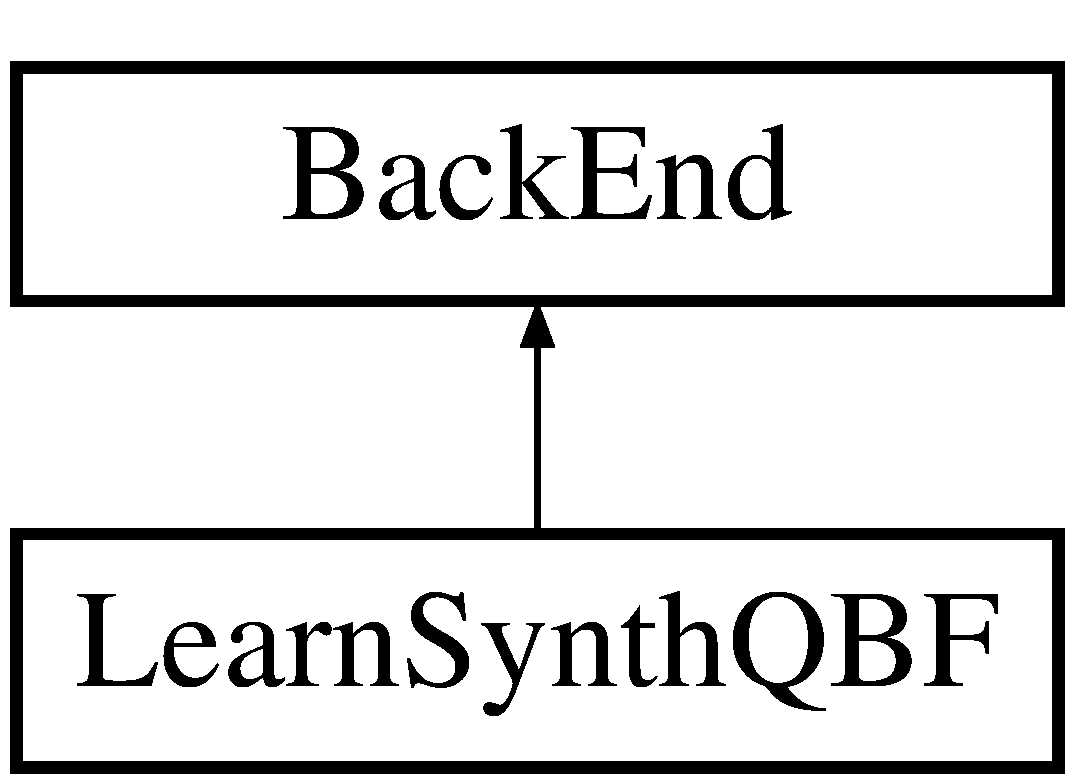
\includegraphics[height=2.000000cm]{classLearnSynthQBF}
\end{center}
\end{figure}
\subsection*{Public Member Functions}
\begin{DoxyCompactItemize}
\item 
\hyperlink{classLearnSynthQBF_ae7f4fe1f847d6af8ecebaa9a9f631b7c}{Learn\-Synth\-Q\-B\-F} (\hyperlink{classCNFImplExtractor}{C\-N\-F\-Impl\-Extractor} $\ast$impl\-\_\-extractor)
\begin{DoxyCompactList}\small\item\em Constructor. \end{DoxyCompactList}\item 
virtual \hyperlink{classLearnSynthQBF_a692e516f27fd78a44884b715688bd7d9}{$\sim$\-Learn\-Synth\-Q\-B\-F} ()
\begin{DoxyCompactList}\small\item\em Destructor. \end{DoxyCompactList}\item 
virtual bool \hyperlink{classLearnSynthQBF_aed85bb2fe317a5fdc7eef71fe598c606}{run} ()
\begin{DoxyCompactList}\small\item\em Executes this back-\/end. \end{DoxyCompactList}\end{DoxyCompactItemize}
\subsection*{Protected Member Functions}
\begin{DoxyCompactItemize}
\item 
bool \hyperlink{classLearnSynthQBF_ae8219ab3e4987775e1d6a006a9d38f4d}{compute\-Winning\-Region} ()
\begin{DoxyCompactList}\small\item\em Computes the winning region and stores the result in \hyperlink{classLearnSynthQBF_a9c6b41f7df5f4ed4bfc5930136fc1152}{winning\-\_\-region\-\_\-}. \end{DoxyCompactList}\item 
bool \hyperlink{classLearnSynthQBF_ac538cd53082bad1c8c45a7e178dfa4cb}{compute\-Winning\-Region\-One} ()
\begin{DoxyCompactList}\small\item\em Uses the standard method to compute the winning region. \end{DoxyCompactList}\item 
bool \hyperlink{classLearnSynthQBF_af8c897056a5018ff1717ea2d76f6cd8f}{compute\-Winning\-Region\-One\-S\-A\-T} ()
\begin{DoxyCompactList}\small\item\em Computes the winning region, using two S\-A\-T-\/solvers to compute counterexamples. \end{DoxyCompactList}\item 
bool \hyperlink{classLearnSynthQBF_a09a9ecb2b77c540cdcc327a35cd15c18}{compute\-Winning\-Region\-All} ()
\begin{DoxyCompactList}\small\item\em Computes the winning region, always computing all counterexample generalizations. \end{DoxyCompactList}\item 
bool \hyperlink{classLearnSynthQBF_a04b8dd6e26d646a6f197afb362168408}{compute\-Counterexample\-Q\-B\-F} (vector$<$ int $>$ \&ce)
\begin{DoxyCompactList}\small\item\em Computes a counterexample-\/state using a Q\-B\-F-\/solver. \end{DoxyCompactList}\item 
bool \hyperlink{classLearnSynthQBF_a3221800bf3f040b66b8a790bab4c82b5}{compute\-Counterexample\-S\-A\-T} (vector$<$ int $>$ \&ce)
\begin{DoxyCompactList}\small\item\em Computes a counterexample-\/state using two competing S\-A\-T-\/solvers. \end{DoxyCompactList}\item 
bool \hyperlink{classLearnSynthQBF_a73856a79be3fb7e260485bcda7c31f80}{compute\-Blocking\-Clause} (vector$<$ int $>$ \&ce, vector$<$ int $>$ \&blocking\-\_\-clause)
\begin{DoxyCompactList}\small\item\em Computes a blocking clause for a counterexample. \end{DoxyCompactList}\item 
bool \hyperlink{classLearnSynthQBF_affa7b4583cc17d01f4c82fd57e763e1f}{compute\-All\-Blocking\-Clauses} (vector$<$ int $>$ \&ce, vector$<$ vector$<$ int $>$ $>$ \&blocking\-\_\-clauses)
\begin{DoxyCompactList}\small\item\em Computes all minimal blocking clauses for a counterexample. \end{DoxyCompactList}\item 
void \hyperlink{classLearnSynthQBF_adf5b9d45d6f69575ed5257fe9a869893}{reduce\-Existing\-Clauses} ()
\begin{DoxyCompactList}\small\item\em Tries to drop literals from clauses in the winning region. \end{DoxyCompactList}\item 
void \hyperlink{classLearnSynthQBF_aa46d02268fe5ea73789280058ec75136}{recompute\-Check\-C\-N\-F} (bool take\-\_\-small\-\_\-win=true)
\begin{DoxyCompactList}\small\item\em Recomputes the \hyperlink{classCNF}{C\-N\-F} (of the Q\-B\-F) that is used for computing counterexamples. \end{DoxyCompactList}\item 
void \hyperlink{classLearnSynthQBF_aa1c6d16c3db9057bfa515b06b7a7ffe9}{recompute\-Gen\-C\-N\-F} (bool take\-\_\-small\-\_\-win=true)
\begin{DoxyCompactList}\small\item\em Recomputes the \hyperlink{classCNF}{C\-N\-F} (of the Q\-B\-F) that is used for generalizing counterexamples. \end{DoxyCompactList}\item 
void \hyperlink{classLearnSynthQBF_a704edaade039b09520815b581fe98b47}{restrict\-To\-States} (vector$<$ int $>$ \&vec) const 
\begin{DoxyCompactList}\small\item\em Restricts a vector of literals (a cube or clause) to state-\/variables only. \end{DoxyCompactList}\item 
bool \hyperlink{classLearnSynthQBF_a9eed607741968f74e31976e8ca40a62f}{generalize\-Counterexample} (vector$<$ int $>$ \&ce, bool check\-\_\-sat=true) const 
\begin{DoxyCompactList}\small\item\em Generalizes a counterexample-\/state by dropping literals. \end{DoxyCompactList}\end{DoxyCompactItemize}
\subsection*{Protected Attributes}
\begin{DoxyCompactItemize}
\item 
\hyperlink{classCNF}{C\-N\-F} \hyperlink{classLearnSynthQBF_a9c6b41f7df5f4ed4bfc5930136fc1152}{winning\-\_\-region\-\_\-}
\begin{DoxyCompactList}\small\item\em The current over-\/approximation of the winning region. \end{DoxyCompactList}\item 
\hyperlink{classCNF}{C\-N\-F} \hyperlink{classLearnSynthQBF_aa9b460cdc140c3969a32ea77982181d2}{winning\-\_\-region\-\_\-large\-\_\-}
\begin{DoxyCompactList}\small\item\em The current over-\/approximation of the winning region in an uncompressed form. \end{DoxyCompactList}\item 
\hyperlink{classLearnStatisticsQBF}{Learn\-Statistics\-Q\-B\-F} \hyperlink{classLearnSynthQBF_a85c46943042fdcfd672ce2251ef49cd9}{statistics\-\_\-}
\begin{DoxyCompactList}\small\item\em Stores and maintains statistics and performance measures. \end{DoxyCompactList}\item 
\hyperlink{classQBFSolver}{Q\-B\-F\-Solver} $\ast$ \hyperlink{classLearnSynthQBF_a8b4c4279f543a0adea992fccf22009f4}{qbf\-\_\-solver\-\_\-}
\begin{DoxyCompactList}\small\item\em The Q\-B\-F-\/solver used for all queries. \end{DoxyCompactList}\item 
vector$<$ pair$<$ \hyperlink{classVarInfo_a64d1da76cf84fe674e5fef9764ef11cf}{Var\-Info\-::\-Var\-Kind}, \\*
\hyperlink{classQBFSolver_ac091e263cb55286cc07b2451bcf4d3c7}{Q\-B\-F\-Solver\-::\-Quant} $>$ $>$ \hyperlink{classLearnSynthQBF_afafe15fef745bb97ac36741cbe00d4c1}{check\-\_\-quant\-\_\-}
\begin{DoxyCompactList}\small\item\em The quantifier prefix of the Q\-B\-F for computing counterexamples. \end{DoxyCompactList}\item 
\hyperlink{classCNF}{C\-N\-F} \hyperlink{classLearnSynthQBF_afe20b32b1b8c07a237322825c91a36f0}{check\-\_\-cnf\-\_\-}
\begin{DoxyCompactList}\small\item\em The \hyperlink{classCNF}{C\-N\-F} matrix of the Q\-B\-F for computing counterexamples. \end{DoxyCompactList}\item 
vector$<$ pair$<$ \hyperlink{classVarInfo_a64d1da76cf84fe674e5fef9764ef11cf}{Var\-Info\-::\-Var\-Kind}, \\*
\hyperlink{classQBFSolver_ac091e263cb55286cc07b2451bcf4d3c7}{Q\-B\-F\-Solver\-::\-Quant} $>$ $>$ \hyperlink{classLearnSynthQBF_a2a6687cca6f45b9684d3bd6e7cc8c20c}{gen\-\_\-quant\-\_\-}
\begin{DoxyCompactList}\small\item\em The quantifier prefix of the Q\-B\-F for generalizing counterexamples. \end{DoxyCompactList}\item 
\hyperlink{classCNF}{C\-N\-F} \hyperlink{classLearnSynthQBF_adb0678a7c034958c31bd5d92615e9859}{generalize\-\_\-clause\-\_\-cnf\-\_\-}
\begin{DoxyCompactList}\small\item\em The \hyperlink{classCNF}{C\-N\-F} matrix of the Q\-B\-F for generalizing counterexamples. \end{DoxyCompactList}\item 
\hyperlink{classSatSolver}{Sat\-Solver} $\ast$ \hyperlink{classLearnSynthQBF_ada2e8c87c0ca0d83c484d6181ea5a788}{solver\-\_\-i\-\_\-}
\begin{DoxyCompactList}\small\item\em The S\-A\-T-\/solver for antagonist moves when using \hyperlink{classLearnSynthQBF_a3221800bf3f040b66b8a790bab4c82b5}{compute\-Counterexample\-S\-A\-T()}. \end{DoxyCompactList}\item 
\hyperlink{classSatSolver}{Sat\-Solver} $\ast$ \hyperlink{classLearnSynthQBF_a14f20d46129ad1fe2db8272348a7e589}{solver\-\_\-ctrl\-\_\-}
\begin{DoxyCompactList}\small\item\em The S\-A\-T-\/solver for protagonist moves when using \hyperlink{classLearnSynthQBF_a3221800bf3f040b66b8a790bab4c82b5}{compute\-Counterexample\-S\-A\-T()}. \end{DoxyCompactList}\item 
vector$<$ int $>$ \hyperlink{classLearnSynthQBF_a227ff215ffb411e57686aa3d8e7f7026}{incremental\-\_\-vars\-\_\-to\-\_\-keep\-\_\-}
\begin{DoxyCompactList}\small\item\em A list of variables the S\-A\-T-\/solver should not optimize away. \end{DoxyCompactList}\item 
bool \hyperlink{classLearnSynthQBF_ae65774a2b9e6137d6ff45cbf755d4843}{solver\-\_\-i\-\_\-precise\-\_\-}
\begin{DoxyCompactList}\small\item\em A flag indicating if solver\-\_\-i\-\_\- is precise. \end{DoxyCompactList}\item 
\hyperlink{classCNFImplExtractor}{C\-N\-F\-Impl\-Extractor} $\ast$ \hyperlink{classLearnSynthQBF_ad34b0c8db41c054eef617e7e9156fad8}{impl\-\_\-extractor\-\_\-}
\begin{DoxyCompactList}\small\item\em The engine to use for circuit extraction. \end{DoxyCompactList}\end{DoxyCompactItemize}
\subsection*{Private Member Functions}
\begin{DoxyCompactItemize}
\item 
\hyperlink{classLearnSynthQBF_ad8d67501811be3fc0366e19df7f8d10a}{Learn\-Synth\-Q\-B\-F} (const \hyperlink{classLearnSynthQBF}{Learn\-Synth\-Q\-B\-F} \&other)
\begin{DoxyCompactList}\small\item\em Copy constructor. \end{DoxyCompactList}\item 
\hyperlink{classLearnSynthQBF}{Learn\-Synth\-Q\-B\-F} \& \hyperlink{classLearnSynthQBF_a143bc7b32f7511ddbdbdec01c2e43578}{operator=} (const \hyperlink{classLearnSynthQBF}{Learn\-Synth\-Q\-B\-F} \&other)
\begin{DoxyCompactList}\small\item\em Assignment operator. \end{DoxyCompactList}\end{DoxyCompactItemize}


\subsection{Detailed Description}
Implements a learning-\/based synthesis using a Q\-B\-F solver. 

The computation of the winning region works as follows. We start with the initial guess that the winning region F is the set of all state states P. In a loop, we first compute a counterexample to the correctness of this guess in form of a state from which the antagonist (controlling the uncontrollable inputs i) can enforce to leave F. The state is represented as a cube over all state-\/variables. Next, this state-\/cube is generalized into a larger region of states by dropping literals as long as the cube contains only states that are winning for the antagonist (and hence must be removed or have already been removed from F). Finally, the generalized cube is removed from F. The next iteration checks for counterexample-\/state on the refined F. This is repeated until no more counterexample-\/states exist (then the specification is realizable and F is a winning region) or the initial state has been removed from F (in which case the specification is unrealizable).

This procedure is implemented in \hyperlink{classLearnSynthQBF_ac538cd53082bad1c8c45a7e178dfa4cb}{compute\-Winning\-Region\-One()}. Some variants of this procedure are implemented in other methods of this class. The method \hyperlink{classLearnSynthQBF_af8c897056a5018ff1717ea2d76f6cd8f}{compute\-Winning\-Region\-One\-S\-A\-T()} uses two S\-A\-T solvers instead of a Q\-B\-F solver to compute a counterexample-\/state. The method \hyperlink{classLearnSynthQBF_a09a9ecb2b77c540cdcc327a35cd15c18}{compute\-Winning\-Region\-All()} computes (and excludes) not only one generalization of the counterexample but all generalizations. Command-\/line parameters (--mode) decide which of these methods to use.

Finally the \hyperlink{classQBFCertImplExtractor}{Q\-B\-F\-Cert\-Impl\-Extractor} is used to extract a circuit.

\begin{DoxyAuthor}{Author}
Robert Koenighofer (\href{mailto:robert.koenighofer@iaik.tugraz.at}{\tt robert.\-koenighofer@iaik.\-tugraz.\-at}) 
\end{DoxyAuthor}
\begin{DoxyVersion}{Version}
1.\-2.\-0 
\end{DoxyVersion}


Definition at line 72 of file Learn\-Synth\-Q\-B\-F.\-h.



\subsection{Constructor \& Destructor Documentation}
\hypertarget{classLearnSynthQBF_ae7f4fe1f847d6af8ecebaa9a9f631b7c}{\index{Learn\-Synth\-Q\-B\-F@{Learn\-Synth\-Q\-B\-F}!Learn\-Synth\-Q\-B\-F@{Learn\-Synth\-Q\-B\-F}}
\index{Learn\-Synth\-Q\-B\-F@{Learn\-Synth\-Q\-B\-F}!LearnSynthQBF@{Learn\-Synth\-Q\-B\-F}}
\subsubsection[{Learn\-Synth\-Q\-B\-F}]{\setlength{\rightskip}{0pt plus 5cm}Learn\-Synth\-Q\-B\-F\-::\-Learn\-Synth\-Q\-B\-F (
\begin{DoxyParamCaption}
\item[{{\bf C\-N\-F\-Impl\-Extractor} $\ast$}]{impl\-\_\-extractor}
\end{DoxyParamCaption}
)}}\label{classLearnSynthQBF_ae7f4fe1f847d6af8ecebaa9a9f631b7c}


Constructor. 


\begin{DoxyParams}{Parameters}
{\em impl\-\_\-extractor} & The engine to use for circuit extraction. It will be deleted by this class. \\
\hline
\end{DoxyParams}


Definition at line 40 of file Learn\-Synth\-Q\-B\-F.\-cpp.



References Q\-B\-F\-Solver\-::\-A, check\-\_\-quant\-\_\-, Var\-Info\-::\-C\-T\-R\-L, Q\-B\-F\-Solver\-::\-E, gen\-\_\-quant\-\_\-, Sat\-Solver\-::inc\-Add\-C\-N\-F(), incremental\-\_\-vars\-\_\-to\-\_\-keep\-\_\-, Var\-Info\-::\-I\-N\-P\-U\-T, A\-I\-G2\-C\-N\-F\-::instance(), Var\-Info\-::\-N\-E\-X\-T\-\_\-\-S\-T\-A\-T\-E, Var\-Info\-::\-P\-R\-E\-S\-\_\-\-S\-T\-A\-T\-E, solver\-\_\-ctrl\-\_\-, solver\-\_\-i\-\_\-, solver\-\_\-i\-\_\-precise\-\_\-, Sat\-Solver\-::start\-Incremental\-Session(), and Var\-Info\-::\-T\-M\-P.

\hypertarget{classLearnSynthQBF_a692e516f27fd78a44884b715688bd7d9}{\index{Learn\-Synth\-Q\-B\-F@{Learn\-Synth\-Q\-B\-F}!$\sim$\-Learn\-Synth\-Q\-B\-F@{$\sim$\-Learn\-Synth\-Q\-B\-F}}
\index{$\sim$\-Learn\-Synth\-Q\-B\-F@{$\sim$\-Learn\-Synth\-Q\-B\-F}!LearnSynthQBF@{Learn\-Synth\-Q\-B\-F}}
\subsubsection[{$\sim$\-Learn\-Synth\-Q\-B\-F}]{\setlength{\rightskip}{0pt plus 5cm}Learn\-Synth\-Q\-B\-F\-::$\sim$\-Learn\-Synth\-Q\-B\-F (
\begin{DoxyParamCaption}
{}
\end{DoxyParamCaption}
)\hspace{0.3cm}{\ttfamily [virtual]}}}\label{classLearnSynthQBF_a692e516f27fd78a44884b715688bd7d9}


Destructor. 



Definition at line 79 of file Learn\-Synth\-Q\-B\-F.\-cpp.



References impl\-\_\-extractor\-\_\-, qbf\-\_\-solver\-\_\-, solver\-\_\-ctrl\-\_\-, and solver\-\_\-i\-\_\-.

\hypertarget{classLearnSynthQBF_ad8d67501811be3fc0366e19df7f8d10a}{\index{Learn\-Synth\-Q\-B\-F@{Learn\-Synth\-Q\-B\-F}!Learn\-Synth\-Q\-B\-F@{Learn\-Synth\-Q\-B\-F}}
\index{Learn\-Synth\-Q\-B\-F@{Learn\-Synth\-Q\-B\-F}!LearnSynthQBF@{Learn\-Synth\-Q\-B\-F}}
\subsubsection[{Learn\-Synth\-Q\-B\-F}]{\setlength{\rightskip}{0pt plus 5cm}Learn\-Synth\-Q\-B\-F\-::\-Learn\-Synth\-Q\-B\-F (
\begin{DoxyParamCaption}
\item[{const {\bf Learn\-Synth\-Q\-B\-F} \&}]{other}
\end{DoxyParamCaption}
)\hspace{0.3cm}{\ttfamily [private]}}}\label{classLearnSynthQBF_ad8d67501811be3fc0366e19df7f8d10a}


Copy constructor. 

The copy constructor is disabled (set private) and not implemented.


\begin{DoxyParams}{Parameters}
{\em other} & The source for creating the copy. \\
\hline
\end{DoxyParams}


\subsection{Member Function Documentation}
\hypertarget{classLearnSynthQBF_affa7b4583cc17d01f4c82fd57e763e1f}{\index{Learn\-Synth\-Q\-B\-F@{Learn\-Synth\-Q\-B\-F}!compute\-All\-Blocking\-Clauses@{compute\-All\-Blocking\-Clauses}}
\index{compute\-All\-Blocking\-Clauses@{compute\-All\-Blocking\-Clauses}!LearnSynthQBF@{Learn\-Synth\-Q\-B\-F}}
\subsubsection[{compute\-All\-Blocking\-Clauses}]{\setlength{\rightskip}{0pt plus 5cm}bool Learn\-Synth\-Q\-B\-F\-::compute\-All\-Blocking\-Clauses (
\begin{DoxyParamCaption}
\item[{vector$<$ int $>$ \&}]{ce, }
\item[{vector$<$ vector$<$ int $>$ $>$ \&}]{blocking\-\_\-clauses}
\end{DoxyParamCaption}
)\hspace{0.3cm}{\ttfamily [protected]}}}\label{classLearnSynthQBF_affa7b4583cc17d01f4c82fd57e763e1f}


Computes all minimal blocking clauses for a counterexample. 

This method is like \hyperlink{classLearnSynthQBF_a73856a79be3fb7e260485bcda7c31f80}{compute\-Blocking\-Clause()}. However, instead of computing just one generalization of the counterexample (and the corresponding blocking clause) it computes all minimal generalizations (and corresponding blocking clauses). It does so using a simple hitting set tree algorithm as presented by \char`\"{}\-Raymond Reiter\-: A Theory of Diagnosis
from First Principles. Artif. Intell. 32(1)\-: 57-\/95 (1987)\char`\"{}.


\begin{DoxyParams}{Parameters}
{\em ce} & The counterexample to block. It is a full or partial cube over the state variables. \\
\hline
{\em blocking\-\_\-clauses} & An empty vector. It is used to store the computed blocking clauses. The counterexample falsifies all blocking clauses in this vector. \\
\hline
\end{DoxyParams}
\begin{DoxyReturn}{Returns}
False if one of the blocking clauses blocks the initial state. This means that the initial state is removed from the winning region, i.\-e., the specification is unrealizable. True is returned otherwise. 
\end{DoxyReturn}


Definition at line 450 of file Learn\-Synth\-Q\-B\-F.\-cpp.



References C\-N\-F\-::add\-Clause(), Utils\-::contains\-Init(), generalize\-\_\-clause\-\_\-cnf\-\_\-, generalize\-Counterexample(), Utils\-::intersection\-Empty(), Utils\-::negate\-Literals(), Learn\-Statistics\-Q\-B\-F\-::notify\-After\-Cube\-Min(), Learn\-Statistics\-Q\-B\-F\-::notify\-Before\-Cube\-Min(), Learn\-Statistics\-Q\-B\-F\-::notify\-Cube\-Min(), Utils\-::remove(), statistics\-\_\-, and Utils\-::swap\-Present\-To\-Next().



Referenced by compute\-Winning\-Region\-All().

\hypertarget{classLearnSynthQBF_a73856a79be3fb7e260485bcda7c31f80}{\index{Learn\-Synth\-Q\-B\-F@{Learn\-Synth\-Q\-B\-F}!compute\-Blocking\-Clause@{compute\-Blocking\-Clause}}
\index{compute\-Blocking\-Clause@{compute\-Blocking\-Clause}!LearnSynthQBF@{Learn\-Synth\-Q\-B\-F}}
\subsubsection[{compute\-Blocking\-Clause}]{\setlength{\rightskip}{0pt plus 5cm}bool Learn\-Synth\-Q\-B\-F\-::compute\-Blocking\-Clause (
\begin{DoxyParamCaption}
\item[{vector$<$ int $>$ \&}]{ce, }
\item[{vector$<$ int $>$ \&}]{blocking\-\_\-clause}
\end{DoxyParamCaption}
)\hspace{0.3cm}{\ttfamily [protected]}}}\label{classLearnSynthQBF_a73856a79be3fb7e260485bcda7c31f80}


Computes a blocking clause for a counterexample. 

A naive blocking clause would be the plain negation of the counterexample. However, in order to boost the overall performance of the algorithm, we generalize the counterexample before we negate it. This is done by dropping literals from the counterexample-\/cube as long as all states in the cube are counterexamples (or have already been removed from the winning region). The method also checks if the blocking clause blocks the initial state.


\begin{DoxyParams}{Parameters}
{\em ce} & The counterexample to block. It is a full or partial cube over the state variables. \\
\hline
{\em blocking\-\_\-clause} & An empty vector. It is used to store the computed blocking clause. The counterexample falsifies the blocking clause. \\
\hline
\end{DoxyParams}
\begin{DoxyReturn}{Returns}
False if the blocking clause blocks the initial state. This means that the initial state is removed from the winning region, i.\-e., the specification is unrealizable. True is returned otherwise. 
\end{DoxyReturn}


Definition at line 432 of file Learn\-Synth\-Q\-B\-F.\-cpp.



References Utils\-::contains\-Init(), generalize\-Counterexample(), L\-\_\-\-D\-B\-G, Utils\-::negate\-Literals(), Learn\-Statistics\-Q\-B\-F\-::notify\-After\-Cube\-Min(), Learn\-Statistics\-Q\-B\-F\-::notify\-Before\-Cube\-Min(), Utils\-::randomize(), and statistics\-\_\-.



Referenced by compute\-Winning\-Region\-One(), and compute\-Winning\-Region\-One\-S\-A\-T().

\hypertarget{classLearnSynthQBF_a04b8dd6e26d646a6f197afb362168408}{\index{Learn\-Synth\-Q\-B\-F@{Learn\-Synth\-Q\-B\-F}!compute\-Counterexample\-Q\-B\-F@{compute\-Counterexample\-Q\-B\-F}}
\index{compute\-Counterexample\-Q\-B\-F@{compute\-Counterexample\-Q\-B\-F}!LearnSynthQBF@{Learn\-Synth\-Q\-B\-F}}
\subsubsection[{compute\-Counterexample\-Q\-B\-F}]{\setlength{\rightskip}{0pt plus 5cm}bool Learn\-Synth\-Q\-B\-F\-::compute\-Counterexample\-Q\-B\-F (
\begin{DoxyParamCaption}
\item[{vector$<$ int $>$ \&}]{ce}
\end{DoxyParamCaption}
)\hspace{0.3cm}{\ttfamily [protected]}}}\label{classLearnSynthQBF_a04b8dd6e26d646a6f197afb362168408}


Computes a counterexample-\/state using a Q\-B\-F-\/solver. 

'Counterexample' here means\-: counterexample to the correctness of the current guess of the winning region. A counterexample is simply a state (represented as cube over the state variables) from which the antagonist can enforce to leave the winning region. This method uses a single call to a Q\-B\-F-\/solver in order to find such a state.


\begin{DoxyParams}{Parameters}
{\em ce} & An empty vector. The computed counterexample is stored in this vector in form of a cube over the state variables. The cube does not necessarily contain all state variables. If some state variables are irrelevant, then they may be omitted. \\
\hline
\end{DoxyParams}
\begin{DoxyReturn}{Returns}
True if a counterexample was found, false if no counterexample exists. 
\end{DoxyReturn}


Definition at line 333 of file Learn\-Synth\-Q\-B\-F.\-cpp.



References check\-\_\-cnf\-\_\-, check\-\_\-quant\-\_\-, Q\-B\-F\-Solver\-::is\-Sat\-Model(), Learn\-Statistics\-Q\-B\-F\-::notify\-After\-Compute\-Cube(), Learn\-Statistics\-Q\-B\-F\-::notify\-Before\-Compute\-Cube(), qbf\-\_\-solver\-\_\-, restrict\-To\-States(), and statistics\-\_\-.



Referenced by compute\-Winning\-Region\-All(), and compute\-Winning\-Region\-One().

\hypertarget{classLearnSynthQBF_a3221800bf3f040b66b8a790bab4c82b5}{\index{Learn\-Synth\-Q\-B\-F@{Learn\-Synth\-Q\-B\-F}!compute\-Counterexample\-S\-A\-T@{compute\-Counterexample\-S\-A\-T}}
\index{compute\-Counterexample\-S\-A\-T@{compute\-Counterexample\-S\-A\-T}!LearnSynthQBF@{Learn\-Synth\-Q\-B\-F}}
\subsubsection[{compute\-Counterexample\-S\-A\-T}]{\setlength{\rightskip}{0pt plus 5cm}bool Learn\-Synth\-Q\-B\-F\-::compute\-Counterexample\-S\-A\-T (
\begin{DoxyParamCaption}
\item[{vector$<$ int $>$ \&}]{ce}
\end{DoxyParamCaption}
)\hspace{0.3cm}{\ttfamily [protected]}}}\label{classLearnSynthQBF_a3221800bf3f040b66b8a790bab4c82b5}


Computes a counterexample-\/state using two competing S\-A\-T-\/solvers. 

'Counterexample' here means\-: counterexample to the correctness of the current guess of the winning region. A counterexample is simply a state (represented as cube over the state variables) from which the antagonist can enforce to leave the winning region. This method uses two competing S\-A\-T-\/solvers in order to find such a state. First, solver \hyperlink{classLearnSynthQBF_ada2e8c87c0ca0d83c484d6181ea5a788}{solver\-\_\-i\-\_\-} finds some input values i that could be chosen by the antagonist in order to leave the \hyperlink{classLearnSynthQBF_a9c6b41f7df5f4ed4bfc5930136fc1152}{winning\-\_\-region\-\_\-}. Next, solver\-\_\-ctrl\-\_\- checks if there exists a response of the protagonist to chose control values c such that the winning region is not left. If no such response exists, then we have found a counterexample. Otherwise, we exclude the state-\/input combination found by \hyperlink{classLearnSynthQBF_ada2e8c87c0ca0d83c484d6181ea5a788}{solver\-\_\-i\-\_\-} and try again.

There is also an optimization which allows to use \hyperlink{classLearnSynthQBF_ada2e8c87c0ca0d83c484d6181ea5a788}{solver\-\_\-i\-\_\-} incrementally\-: The next state-\/copy of the winning region is updated only lazily.


\begin{DoxyParams}{Parameters}
{\em ce} & An empty vector. The computed counterexample is stored in this vector in form of a cube over the state variables. The cube does not necessarily contain all state variables. If some state variables are irrelevant, then they may be omitted. \\
\hline
\end{DoxyParams}
\begin{DoxyReturn}{Returns}
True if a counterexample was found, false if no counterexample exists. 
\end{DoxyReturn}


Definition at line 345 of file Learn\-Synth\-Q\-B\-F.\-cpp.



References C\-N\-F\-::add\-C\-N\-F(), Utils\-::compress\-State\-C\-N\-F(), Var\-Info\-::\-C\-T\-R\-L, Utils\-::extract(), Var\-Manager\-::get\-Vars\-Of\-Type(), Sat\-Solver\-::inc\-Add\-Clause(), Sat\-Solver\-::inc\-Add\-C\-N\-F(), Sat\-Solver\-::inc\-Is\-Sat\-Model\-Or\-Core(), incremental\-\_\-vars\-\_\-to\-\_\-keep\-\_\-, Var\-Info\-::\-I\-N\-P\-U\-T, Var\-Manager\-::instance(), A\-I\-G2\-C\-N\-F\-::instance(), L\-\_\-\-D\-B\-G, M\-A\-S\-S\-E\-R\-T, C\-N\-F\-::negate(), Learn\-Statistics\-Q\-B\-F\-::notify\-After\-Compute\-Cube(), Learn\-Statistics\-Q\-B\-F\-::notify\-Before\-Compute\-Cube(), Var\-Info\-::\-P\-R\-E\-S\-\_\-\-S\-T\-A\-T\-E, solver\-\_\-ctrl\-\_\-, solver\-\_\-i\-\_\-, solver\-\_\-i\-\_\-precise\-\_\-, Sat\-Solver\-::start\-Incremental\-Session(), statistics\-\_\-, C\-N\-F\-::swap\-Present\-To\-Next(), and winning\-\_\-region\-\_\-.



Referenced by compute\-Winning\-Region\-One\-S\-A\-T().

\hypertarget{classLearnSynthQBF_ae8219ab3e4987775e1d6a006a9d38f4d}{\index{Learn\-Synth\-Q\-B\-F@{Learn\-Synth\-Q\-B\-F}!compute\-Winning\-Region@{compute\-Winning\-Region}}
\index{compute\-Winning\-Region@{compute\-Winning\-Region}!LearnSynthQBF@{Learn\-Synth\-Q\-B\-F}}
\subsubsection[{compute\-Winning\-Region}]{\setlength{\rightskip}{0pt plus 5cm}bool Learn\-Synth\-Q\-B\-F\-::compute\-Winning\-Region (
\begin{DoxyParamCaption}
{}
\end{DoxyParamCaption}
)\hspace{0.3cm}{\ttfamily [protected]}}}\label{classLearnSynthQBF_ae8219ab3e4987775e1d6a006a9d38f4d}


Computes the winning region and stores the result in \hyperlink{classLearnSynthQBF_a9c6b41f7df5f4ed4bfc5930136fc1152}{winning\-\_\-region\-\_\-}. 

Depending on the command-\/line parameters (--mode) this method calls one of 
\begin{DoxyItemize}
\item \hyperlink{classLearnSynthQBF_ac538cd53082bad1c8c45a7e178dfa4cb}{compute\-Winning\-Region\-One()} 
\item \hyperlink{classLearnSynthQBF_af8c897056a5018ff1717ea2d76f6cd8f}{compute\-Winning\-Region\-One\-S\-A\-T()} 
\item \hyperlink{classLearnSynthQBF_a09a9ecb2b77c540cdcc327a35cd15c18}{compute\-Winning\-Region\-All()} 
\end{DoxyItemize}

\begin{DoxyReturn}{Returns}
True if the specification was realizable, false otherwise. 
\end{DoxyReturn}


Definition at line 125 of file Learn\-Synth\-Q\-B\-F.\-cpp.



References compute\-Winning\-Region\-All(), compute\-Winning\-Region\-One(), compute\-Winning\-Region\-One\-S\-A\-T(), and Options\-::instance().



Referenced by run().

\hypertarget{classLearnSynthQBF_a09a9ecb2b77c540cdcc327a35cd15c18}{\index{Learn\-Synth\-Q\-B\-F@{Learn\-Synth\-Q\-B\-F}!compute\-Winning\-Region\-All@{compute\-Winning\-Region\-All}}
\index{compute\-Winning\-Region\-All@{compute\-Winning\-Region\-All}!LearnSynthQBF@{Learn\-Synth\-Q\-B\-F}}
\subsubsection[{compute\-Winning\-Region\-All}]{\setlength{\rightskip}{0pt plus 5cm}bool Learn\-Synth\-Q\-B\-F\-::compute\-Winning\-Region\-All (
\begin{DoxyParamCaption}
{}
\end{DoxyParamCaption}
)\hspace{0.3cm}{\ttfamily [protected]}}}\label{classLearnSynthQBF_a09a9ecb2b77c540cdcc327a35cd15c18}


Computes the winning region, always computing all counterexample generalizations. 

The working principle is the same as for \hyperlink{classLearnSynthQBF_ac538cd53082bad1c8c45a7e178dfa4cb}{compute\-Winning\-Region\-One()}. The only difference is that this method computes and excludes all counterexample generalizations instead of just one.

\begin{DoxyReturn}{Returns}
True if the specification was realizable, false otherwise. 
\end{DoxyReturn}


Definition at line 267 of file Learn\-Synth\-Q\-B\-F.\-cpp.



References C\-N\-F\-::add\-Clause\-And\-Simplify(), check\-\_\-cnf\-\_\-, C\-N\-F\-::clear(), Utils\-::compress\-State\-C\-N\-F(), compute\-All\-Blocking\-Clauses(), compute\-Counterexample\-Q\-B\-F(), Var\-Info\-::\-C\-T\-R\-L, Logger\-::\-D\-B\-G, Utils\-::debug\-Print(), generalize\-\_\-clause\-\_\-cnf\-\_\-, C\-N\-F\-::get\-Nr\-Of\-Clauses(), C\-N\-F\-::get\-Nr\-Of\-Lits(), A\-I\-G2\-C\-N\-F\-::get\-Safe\-States(), Var\-Manager\-::get\-Vars\-Of\-Type(), Var\-Info\-::\-I\-N\-P\-U\-T, Var\-Manager\-::instance(), Logger\-::instance(), A\-I\-G2\-C\-N\-F\-::instance(), Logger\-::is\-Enabled(), L\-\_\-\-D\-B\-G, Learn\-Statistics\-Q\-B\-F\-::log\-Statistics(), Var\-Info\-::\-P\-R\-E\-S\-\_\-\-S\-T\-A\-T\-E, recompute\-Check\-C\-N\-F(), recompute\-Gen\-C\-N\-F(), reduce\-Existing\-Clauses(), statistics\-\_\-, winning\-\_\-region\-\_\-, and winning\-\_\-region\-\_\-large\-\_\-.



Referenced by compute\-Winning\-Region().

\hypertarget{classLearnSynthQBF_ac538cd53082bad1c8c45a7e178dfa4cb}{\index{Learn\-Synth\-Q\-B\-F@{Learn\-Synth\-Q\-B\-F}!compute\-Winning\-Region\-One@{compute\-Winning\-Region\-One}}
\index{compute\-Winning\-Region\-One@{compute\-Winning\-Region\-One}!LearnSynthQBF@{Learn\-Synth\-Q\-B\-F}}
\subsubsection[{compute\-Winning\-Region\-One}]{\setlength{\rightskip}{0pt plus 5cm}bool Learn\-Synth\-Q\-B\-F\-::compute\-Winning\-Region\-One (
\begin{DoxyParamCaption}
{}
\end{DoxyParamCaption}
)\hspace{0.3cm}{\ttfamily [protected]}}}\label{classLearnSynthQBF_ac538cd53082bad1c8c45a7e178dfa4cb}


Uses the standard method to compute the winning region. 

This standard method works as follows. We start with the initial guess that the winning region F is the set of all state states P. In a loop, we first compute a counterexample to the correctness of this guess in form of a state from which the antagonist (controlling the uncontrollable inputs i) can enforce to leave F. The state is represented as a cube over all state-\/variables. Next, this state-\/cube is generalized into a larger region of states by dropping literals as long as the cube contains only states that are winning for the antagonist (and hence must be removed or have already been removed from F). Finally, the generalized cube is removed from F. The next iteration checks for counterexample-\/state on the refined F. This is repeated until no more counterexample-\/states exist (then the specification is realizable and F is a winning region) or the initial state has been removed from F (in which case the specification is unrealizable).

\begin{DoxyReturn}{Returns}
True if the specification was realizable, false otherwise. 
\end{DoxyReturn}


Definition at line 135 of file Learn\-Synth\-Q\-B\-F.\-cpp.



References C\-N\-F\-::add\-Clause\-And\-Simplify(), check\-\_\-cnf\-\_\-, C\-N\-F\-::clear(), Utils\-::compress\-State\-C\-N\-F(), compute\-Blocking\-Clause(), compute\-Counterexample\-Q\-B\-F(), Var\-Info\-::\-C\-T\-R\-L, Logger\-::\-D\-B\-G, Utils\-::debug\-Print(), generalize\-\_\-clause\-\_\-cnf\-\_\-, C\-N\-F\-::get\-Nr\-Of\-Clauses(), C\-N\-F\-::get\-Nr\-Of\-Lits(), A\-I\-G2\-C\-N\-F\-::get\-Safe\-States(), Var\-Manager\-::get\-Vars\-Of\-Type(), Var\-Info\-::\-I\-N\-P\-U\-T, Var\-Manager\-::instance(), Logger\-::instance(), A\-I\-G2\-C\-N\-F\-::instance(), Logger\-::is\-Enabled(), L\-\_\-\-D\-B\-G, Learn\-Statistics\-Q\-B\-F\-::log\-Statistics(), Var\-Info\-::\-P\-R\-E\-S\-\_\-\-S\-T\-A\-T\-E, recompute\-Check\-C\-N\-F(), recompute\-Gen\-C\-N\-F(), statistics\-\_\-, Utils\-::swap\-Present\-To\-Next(), winning\-\_\-region\-\_\-, and winning\-\_\-region\-\_\-large\-\_\-.



Referenced by compute\-Winning\-Region().

\hypertarget{classLearnSynthQBF_af8c897056a5018ff1717ea2d76f6cd8f}{\index{Learn\-Synth\-Q\-B\-F@{Learn\-Synth\-Q\-B\-F}!compute\-Winning\-Region\-One\-S\-A\-T@{compute\-Winning\-Region\-One\-S\-A\-T}}
\index{compute\-Winning\-Region\-One\-S\-A\-T@{compute\-Winning\-Region\-One\-S\-A\-T}!LearnSynthQBF@{Learn\-Synth\-Q\-B\-F}}
\subsubsection[{compute\-Winning\-Region\-One\-S\-A\-T}]{\setlength{\rightskip}{0pt plus 5cm}bool Learn\-Synth\-Q\-B\-F\-::compute\-Winning\-Region\-One\-S\-A\-T (
\begin{DoxyParamCaption}
{}
\end{DoxyParamCaption}
)\hspace{0.3cm}{\ttfamily [protected]}}}\label{classLearnSynthQBF_af8c897056a5018ff1717ea2d76f6cd8f}


Computes the winning region, using two S\-A\-T-\/solvers to compute counterexamples. 

The working principle is the same as for \hyperlink{classLearnSynthQBF_ac538cd53082bad1c8c45a7e178dfa4cb}{compute\-Winning\-Region\-One()}. The only difference is that counterexample-\/states (states from which the antagonist controlling the inputs i can enforce to leave the winning region) are computed using two competing S\-A\-T-\/solvers instead of a Q\-B\-F-\/solver.

\begin{DoxyReturn}{Returns}
True if the specification was realizable, false otherwise. 
\end{DoxyReturn}


Definition at line 204 of file Learn\-Synth\-Q\-B\-F.\-cpp.



References C\-N\-F\-::add\-Clause\-And\-Simplify(), check\-\_\-cnf\-\_\-, C\-N\-F\-::clear(), compute\-Blocking\-Clause(), compute\-Counterexample\-S\-A\-T(), Var\-Info\-::\-C\-T\-R\-L, Logger\-::\-D\-B\-G, Utils\-::debug\-Print(), generalize\-\_\-clause\-\_\-cnf\-\_\-, C\-N\-F\-::get\-Nr\-Of\-Clauses(), C\-N\-F\-::get\-Nr\-Of\-Lits(), A\-I\-G2\-C\-N\-F\-::get\-Safe\-States(), Var\-Manager\-::get\-Vars\-Of\-Type(), Sat\-Solver\-::inc\-Add\-Clause(), Var\-Info\-::\-I\-N\-P\-U\-T, Var\-Manager\-::instance(), Logger\-::instance(), A\-I\-G2\-C\-N\-F\-::instance(), Logger\-::is\-Enabled(), L\-\_\-\-D\-B\-G, Learn\-Statistics\-Q\-B\-F\-::log\-Statistics(), Var\-Info\-::\-P\-R\-E\-S\-\_\-\-S\-T\-A\-T\-E, recompute\-Gen\-C\-N\-F(), solver\-\_\-ctrl\-\_\-, solver\-\_\-i\-\_\-, statistics\-\_\-, Utils\-::swap\-Present\-To\-Next(), winning\-\_\-region\-\_\-, and winning\-\_\-region\-\_\-large\-\_\-.



Referenced by compute\-Winning\-Region().

\hypertarget{classLearnSynthQBF_a9eed607741968f74e31976e8ca40a62f}{\index{Learn\-Synth\-Q\-B\-F@{Learn\-Synth\-Q\-B\-F}!generalize\-Counterexample@{generalize\-Counterexample}}
\index{generalize\-Counterexample@{generalize\-Counterexample}!LearnSynthQBF@{Learn\-Synth\-Q\-B\-F}}
\subsubsection[{generalize\-Counterexample}]{\setlength{\rightskip}{0pt plus 5cm}bool Learn\-Synth\-Q\-B\-F\-::generalize\-Counterexample (
\begin{DoxyParamCaption}
\item[{vector$<$ int $>$ \&}]{ce, }
\item[{bool}]{check\-\_\-sat = {\ttfamily true}}
\end{DoxyParamCaption}
) const\hspace{0.3cm}{\ttfamily [protected]}}}\label{classLearnSynthQBF_a9eed607741968f74e31976e8ca40a62f}


Generalizes a counterexample-\/state by dropping literals. 

This method generalizes a counterexample-\/state (a cube over the present-\/state variables) by dropping literals as long as all states in the cube are counterexamples (or have already been removed from the winning region). Optionally, this method also checks if the passed vector is a valid (generalization of a) counterexample.


\begin{DoxyParams}{Parameters}
{\em ce} & The counterexample to generalize (it will be overwritten by its own generalization). This is a complete or partial cube over the present state variables. \\
\hline
{\em check\-\_\-sat} & If set to true, then this method checks if the passed counterexample vector is indeed a valid (generalization of a) counterexample. If set to false, then this step is skipped. If this parameter is true and the passed vector is not a valid counterexample, then it will not be modified. \\
\hline
\end{DoxyParams}
\begin{DoxyReturn}{Returns}
True if the passed vector is a valid (generalization of a) counterexample, or if the check was skipped by setting check\-\_\-sat = false. False is returned only if the check was performed (check\-\_\-sat = true) and the passed vector is not a valid counterexample. 
\end{DoxyReturn}


Definition at line 627 of file Learn\-Synth\-Q\-B\-F.\-cpp.



References C\-N\-F\-::add\-Cube(), C\-N\-F\-::add\-Neg\-Cube\-As\-Clause(), gen\-\_\-quant\-\_\-, generalize\-\_\-clause\-\_\-cnf\-\_\-, Q\-B\-F\-Solver\-::is\-Sat(), qbf\-\_\-solver\-\_\-, Utils\-::remove(), Utils\-::sort(), and Utils\-::swap\-Present\-To\-Next().



Referenced by compute\-All\-Blocking\-Clauses(), and compute\-Blocking\-Clause().

\hypertarget{classLearnSynthQBF_a143bc7b32f7511ddbdbdec01c2e43578}{\index{Learn\-Synth\-Q\-B\-F@{Learn\-Synth\-Q\-B\-F}!operator=@{operator=}}
\index{operator=@{operator=}!LearnSynthQBF@{Learn\-Synth\-Q\-B\-F}}
\subsubsection[{operator=}]{\setlength{\rightskip}{0pt plus 5cm}{\bf Learn\-Synth\-Q\-B\-F}\& Learn\-Synth\-Q\-B\-F\-::operator= (
\begin{DoxyParamCaption}
\item[{const {\bf Learn\-Synth\-Q\-B\-F} \&}]{other}
\end{DoxyParamCaption}
)\hspace{0.3cm}{\ttfamily [private]}}}\label{classLearnSynthQBF_a143bc7b32f7511ddbdbdec01c2e43578}


Assignment operator. 

The assignment operator is disabled (set private) and not implemented.


\begin{DoxyParams}{Parameters}
{\em other} & The source for creating the copy. \\
\hline
\end{DoxyParams}
\begin{DoxyReturn}{Returns}
The result of the assignment, i.\-e, $\ast$this. 
\end{DoxyReturn}
\hypertarget{classLearnSynthQBF_aa46d02268fe5ea73789280058ec75136}{\index{Learn\-Synth\-Q\-B\-F@{Learn\-Synth\-Q\-B\-F}!recompute\-Check\-C\-N\-F@{recompute\-Check\-C\-N\-F}}
\index{recompute\-Check\-C\-N\-F@{recompute\-Check\-C\-N\-F}!LearnSynthQBF@{Learn\-Synth\-Q\-B\-F}}
\subsubsection[{recompute\-Check\-C\-N\-F}]{\setlength{\rightskip}{0pt plus 5cm}void Learn\-Synth\-Q\-B\-F\-::recompute\-Check\-C\-N\-F (
\begin{DoxyParamCaption}
\item[{bool}]{take\-\_\-small\-\_\-win = {\ttfamily true}}
\end{DoxyParamCaption}
)\hspace{0.3cm}{\ttfamily [protected]}}}\label{classLearnSynthQBF_aa46d02268fe5ea73789280058ec75136}


Recomputes the \hyperlink{classCNF}{C\-N\-F} (of the Q\-B\-F) that is used for computing counterexamples. 

The \hyperlink{classCNF}{C\-N\-F} used for computing counterexamples is F \& T \& !\-F', where F is the \hyperlink{classLearnSynthQBF_a9c6b41f7df5f4ed4bfc5930136fc1152}{winning\-\_\-region\-\_\-}. The result is stored in \hyperlink{classLearnSynthQBF_afe20b32b1b8c07a237322825c91a36f0}{check\-\_\-cnf\-\_\-}. Since F is constantly updated with new clauses, \hyperlink{classLearnSynthQBF_afe20b32b1b8c07a237322825c91a36f0}{check\-\_\-cnf\-\_\-} needs to be updated as well. In an old version, we updated the \hyperlink{classLearnSynthQBF_afe20b32b1b8c07a237322825c91a36f0}{check\-\_\-cnf\-\_\-} in place, modifying only the clauses that need to be modified. This gives quite ugly code. Since this operation is not performance critical (compared to Q\-B\-F-\/solving), we now recompute check\-\_\-cnf\-\_\- completely in each iteration.


\begin{DoxyParams}{Parameters}
{\em take\-\_\-small\-\_\-win} & If this parameter is true (or omitted) the \hyperlink{classLearnSynthQBF_a9c6b41f7df5f4ed4bfc5930136fc1152}{winning\-\_\-region\-\_\-} is used to compute the \hyperlink{classLearnSynthQBF_afe20b32b1b8c07a237322825c91a36f0}{check\-\_\-cnf\-\_\-}. Otherwise, the \hyperlink{classLearnSynthQBF_aa9b460cdc140c3969a32ea77982181d2}{winning\-\_\-region\-\_\-large\-\_\-} is used. The difference between these two winning region versions is as follows. From time to we remove redundant clauses (clauses implied by other clauses) from \hyperlink{classLearnSynthQBF_a9c6b41f7df5f4ed4bfc5930136fc1152}{winning\-\_\-region\-\_\-} but not from \hyperlink{classLearnSynthQBF_aa9b460cdc140c3969a32ea77982181d2}{winning\-\_\-region\-\_\-large\-\_\-}. Hence, \hyperlink{classLearnSynthQBF_a9c6b41f7df5f4ed4bfc5930136fc1152}{winning\-\_\-region\-\_\-} is often smaller, but \hyperlink{classLearnSynthQBF_aa9b460cdc140c3969a32ea77982181d2}{winning\-\_\-region\-\_\-large\-\_\-} may contain clauses the solver may have to learn when using \hyperlink{classLearnSynthQBF_a9c6b41f7df5f4ed4bfc5930136fc1152}{winning\-\_\-region\-\_\-}. \\
\hline
\end{DoxyParams}


Definition at line 565 of file Learn\-Synth\-Q\-B\-F.\-cpp.



References C\-N\-F\-::add\-C\-N\-F(), check\-\_\-cnf\-\_\-, C\-N\-F\-::clear(), A\-I\-G2\-C\-N\-F\-::instance(), C\-N\-F\-::negate(), Var\-Manager\-::reset\-To\-Last\-Push(), C\-N\-F\-::swap\-Present\-To\-Next(), winning\-\_\-region\-\_\-, and winning\-\_\-region\-\_\-large\-\_\-.



Referenced by compute\-Winning\-Region\-All(), and compute\-Winning\-Region\-One().

\hypertarget{classLearnSynthQBF_aa1c6d16c3db9057bfa515b06b7a7ffe9}{\index{Learn\-Synth\-Q\-B\-F@{Learn\-Synth\-Q\-B\-F}!recompute\-Gen\-C\-N\-F@{recompute\-Gen\-C\-N\-F}}
\index{recompute\-Gen\-C\-N\-F@{recompute\-Gen\-C\-N\-F}!LearnSynthQBF@{Learn\-Synth\-Q\-B\-F}}
\subsubsection[{recompute\-Gen\-C\-N\-F}]{\setlength{\rightskip}{0pt plus 5cm}void Learn\-Synth\-Q\-B\-F\-::recompute\-Gen\-C\-N\-F (
\begin{DoxyParamCaption}
\item[{bool}]{take\-\_\-small\-\_\-win = {\ttfamily true}}
\end{DoxyParamCaption}
)\hspace{0.3cm}{\ttfamily [protected]}}}\label{classLearnSynthQBF_aa1c6d16c3db9057bfa515b06b7a7ffe9}


Recomputes the \hyperlink{classCNF}{C\-N\-F} (of the Q\-B\-F) that is used for generalizing counterexamples. 

The \hyperlink{classCNF}{C\-N\-F} used for generalizing counterexamples is F \& T \& F', where F is the \hyperlink{classLearnSynthQBF_a9c6b41f7df5f4ed4bfc5930136fc1152}{winning\-\_\-region\-\_\-}. The result is stored in \hyperlink{classLearnSynthQBF_adb0678a7c034958c31bd5d92615e9859}{generalize\-\_\-clause\-\_\-cnf\-\_\-}. Since F is constantly updated with new clauses, \hyperlink{classLearnSynthQBF_adb0678a7c034958c31bd5d92615e9859}{generalize\-\_\-clause\-\_\-cnf\-\_\-} needs to be updated as well. In an old version, we updated the \hyperlink{classLearnSynthQBF_adb0678a7c034958c31bd5d92615e9859}{generalize\-\_\-clause\-\_\-cnf\-\_\-} in place. This results in ugly code at some places (especially when the \hyperlink{classLearnSynthQBF_a9c6b41f7df5f4ed4bfc5930136fc1152}{winning\-\_\-region\-\_\-} is compressed or simplified). Since this operation is not performance critical (compared to Q\-B\-F-\/solving), we now recompute \hyperlink{classLearnSynthQBF_adb0678a7c034958c31bd5d92615e9859}{generalize\-\_\-clause\-\_\-cnf\-\_\-} completely in each iteration.


\begin{DoxyParams}{Parameters}
{\em take\-\_\-small\-\_\-win} & If this parameter is true (or omitted) the \hyperlink{classLearnSynthQBF_a9c6b41f7df5f4ed4bfc5930136fc1152}{winning\-\_\-region\-\_\-} is used to compute the \hyperlink{classLearnSynthQBF_adb0678a7c034958c31bd5d92615e9859}{generalize\-\_\-clause\-\_\-cnf\-\_\-}. Otherwise, the \hyperlink{classLearnSynthQBF_aa9b460cdc140c3969a32ea77982181d2}{winning\-\_\-region\-\_\-large\-\_\-} is used. The difference between these two winning region versions is as follows. From time to we remove redundant clauses (clauses implied by other clauses) from \hyperlink{classLearnSynthQBF_a9c6b41f7df5f4ed4bfc5930136fc1152}{winning\-\_\-region\-\_\-} but not from \hyperlink{classLearnSynthQBF_aa9b460cdc140c3969a32ea77982181d2}{winning\-\_\-region\-\_\-large\-\_\-}. Hence, \hyperlink{classLearnSynthQBF_a9c6b41f7df5f4ed4bfc5930136fc1152}{winning\-\_\-region\-\_\-} is often smaller, but \hyperlink{classLearnSynthQBF_aa9b460cdc140c3969a32ea77982181d2}{winning\-\_\-region\-\_\-large\-\_\-} may contain clauses the solver may have to learn when using \hyperlink{classLearnSynthQBF_a9c6b41f7df5f4ed4bfc5930136fc1152}{winning\-\_\-region\-\_\-}. \\
\hline
\end{DoxyParams}


Definition at line 588 of file Learn\-Synth\-Q\-B\-F.\-cpp.



References C\-N\-F\-::add\-C\-N\-F(), C\-N\-F\-::clear(), generalize\-\_\-clause\-\_\-cnf\-\_\-, A\-I\-G2\-C\-N\-F\-::instance(), C\-N\-F\-::swap\-Present\-To\-Next(), winning\-\_\-region\-\_\-, and winning\-\_\-region\-\_\-large\-\_\-.



Referenced by compute\-Winning\-Region\-All(), compute\-Winning\-Region\-One(), and compute\-Winning\-Region\-One\-S\-A\-T().

\hypertarget{classLearnSynthQBF_adf5b9d45d6f69575ed5257fe9a869893}{\index{Learn\-Synth\-Q\-B\-F@{Learn\-Synth\-Q\-B\-F}!reduce\-Existing\-Clauses@{reduce\-Existing\-Clauses}}
\index{reduce\-Existing\-Clauses@{reduce\-Existing\-Clauses}!LearnSynthQBF@{Learn\-Synth\-Q\-B\-F}}
\subsubsection[{reduce\-Existing\-Clauses}]{\setlength{\rightskip}{0pt plus 5cm}void Learn\-Synth\-Q\-B\-F\-::reduce\-Existing\-Clauses (
\begin{DoxyParamCaption}
{}
\end{DoxyParamCaption}
)\hspace{0.3cm}{\ttfamily [protected]}}}\label{classLearnSynthQBF_adf5b9d45d6f69575ed5257fe9a869893}


Tries to drop literals from clauses in the winning region. 

This method examines all clauses (in \hyperlink{classLearnSynthQBF_a9c6b41f7df5f4ed4bfc5930136fc1152}{winning\-\_\-region\-\_\-}) that have already been computed and checks if more literals can be dropped. This is done in the same way as for dropping literals when generalizing a counterexample.

The intuition behind this method is that, even if a literal could not be dropped before, it could be dropped at a later point in time because the winning region has been refined in the meantime. However, in practice, typically only very few additional literals can be dropped, so this method often does not pay off. 

Definition at line 532 of file Learn\-Synth\-Q\-B\-F.\-cpp.



References C\-N\-F\-::add\-Clause\-And\-Simplify(), C\-N\-F\-::add\-Neg\-Clause\-As\-Cube(), gen\-\_\-quant\-\_\-, generalize\-\_\-clause\-\_\-cnf\-\_\-, C\-N\-F\-::get\-Clauses(), C\-N\-F\-::get\-Nr\-Of\-Clauses(), C\-N\-F\-::get\-Nr\-Of\-Lits(), Q\-B\-F\-Solver\-::is\-Sat(), L\-\_\-\-D\-B\-G, Learn\-Statistics\-Q\-B\-F\-::notify\-After\-Cube\-Min(), Learn\-Statistics\-Q\-B\-F\-::notify\-Before\-Cube\-Min(), qbf\-\_\-solver\-\_\-, Utils\-::remove(), statistics\-\_\-, winning\-\_\-region\-\_\-, and winning\-\_\-region\-\_\-large\-\_\-.



Referenced by compute\-Winning\-Region\-All().

\hypertarget{classLearnSynthQBF_a704edaade039b09520815b581fe98b47}{\index{Learn\-Synth\-Q\-B\-F@{Learn\-Synth\-Q\-B\-F}!restrict\-To\-States@{restrict\-To\-States}}
\index{restrict\-To\-States@{restrict\-To\-States}!LearnSynthQBF@{Learn\-Synth\-Q\-B\-F}}
\subsubsection[{restrict\-To\-States}]{\setlength{\rightskip}{0pt plus 5cm}void Learn\-Synth\-Q\-B\-F\-::restrict\-To\-States (
\begin{DoxyParamCaption}
\item[{vector$<$ int $>$ \&}]{vec}
\end{DoxyParamCaption}
) const\hspace{0.3cm}{\ttfamily [protected]}}}\label{classLearnSynthQBF_a704edaade039b09520815b581fe98b47}


Restricts a vector of literals (a cube or clause) to state-\/variables only. 

That is, all literals that do not talk about present state variables are removed.


\begin{DoxyParams}{Parameters}
{\em vec} & The vector of literals (the cube or clause) to restricts to state-\/variables only. \\
\hline
\end{DoxyParams}


Definition at line 608 of file Learn\-Synth\-Q\-B\-F.\-cpp.



References Var\-Manager\-::get\-Info(), Var\-Info\-::get\-Kind(), Var\-Manager\-::get\-Pres\-Error\-State\-Var(), Var\-Manager\-::instance(), and Var\-Info\-::\-P\-R\-E\-S\-\_\-\-S\-T\-A\-T\-E.



Referenced by compute\-Counterexample\-Q\-B\-F().

\hypertarget{classLearnSynthQBF_aed85bb2fe317a5fdc7eef71fe598c606}{\index{Learn\-Synth\-Q\-B\-F@{Learn\-Synth\-Q\-B\-F}!run@{run}}
\index{run@{run}!LearnSynthQBF@{Learn\-Synth\-Q\-B\-F}}
\subsubsection[{run}]{\setlength{\rightskip}{0pt plus 5cm}bool Learn\-Synth\-Q\-B\-F\-::run (
\begin{DoxyParamCaption}
{}
\end{DoxyParamCaption}
)\hspace{0.3cm}{\ttfamily [virtual]}}}\label{classLearnSynthQBF_aed85bb2fe317a5fdc7eef71fe598c606}


Executes this back-\/end. 

The computation of the winning region works as follows. We start with the initial guess that the winning region F is the set of all state states P. In a loop, we first compute a counterexample to the correctness of this guess in form of a state from which the antagonist (controlling the uncontrollable inputs i) can enforce to leave F. The state is represented as a cube over all state-\/variables. Next, this state-\/cube is generalized into a larger region of states by dropping literals as long as the cube contains only states that are winning for the antagonist (and hence must be removed or have already been removed from F). Finally, the generalized cube is removed from F. The next iteration checks for counterexample-\/state on the refined F. This is repeated until no more counterexample-\/states exist (then the specification is realizable and F is a winning region) or the initial state has been removed from F (in which case the specification is unrealizable).

Command-\/line parameters (--mode) are used to select different variants of this method. There is 
\begin{DoxyItemize}
\item the standard method as described above, 
\item a variant which computes counterexamples using two S\-A\-T-\/solvers instead of a Q\-B\-F solver, 
\item a variant which computes and excludes all counterexample-\/generalizations instead of just one. 
\end{DoxyItemize}

\begin{DoxyReturn}{Returns}
True if the specification was realizable, false otherwise. 
\end{DoxyReturn}


Implements \hyperlink{classBackEnd_a099e717dc71e9cc2d838b1ca86340590}{Back\-End}.



Definition at line 92 of file Learn\-Synth\-Q\-B\-F.\-cpp.



References compute\-Winning\-Region(), Utils\-::debug\-Check\-Win\-Reg(), C\-N\-F\-Impl\-Extractor\-::extract\-Circuit(), impl\-\_\-extractor\-\_\-, Var\-Manager\-::instance(), Options\-::instance(), L\-\_\-\-I\-N\-F, L\-\_\-\-R\-E\-S, C\-N\-F\-Impl\-Extractor\-::log\-Statistics(), Learn\-Statistics\-Q\-B\-F\-::log\-Statistics(), Learn\-Statistics\-Q\-B\-F\-::notify\-Win\-Reg\-End(), Learn\-Statistics\-Q\-B\-F\-::notify\-Win\-Reg\-Start(), Var\-Manager\-::push(), statistics\-\_\-, and winning\-\_\-region\-\_\-.



\subsection{Member Data Documentation}
\hypertarget{classLearnSynthQBF_afe20b32b1b8c07a237322825c91a36f0}{\index{Learn\-Synth\-Q\-B\-F@{Learn\-Synth\-Q\-B\-F}!check\-\_\-cnf\-\_\-@{check\-\_\-cnf\-\_\-}}
\index{check\-\_\-cnf\-\_\-@{check\-\_\-cnf\-\_\-}!LearnSynthQBF@{Learn\-Synth\-Q\-B\-F}}
\subsubsection[{check\-\_\-cnf\-\_\-}]{\setlength{\rightskip}{0pt plus 5cm}{\bf C\-N\-F} Learn\-Synth\-Q\-B\-F\-::check\-\_\-cnf\-\_\-\hspace{0.3cm}{\ttfamily [protected]}}}\label{classLearnSynthQBF_afe20b32b1b8c07a237322825c91a36f0}


The \hyperlink{classCNF}{C\-N\-F} matrix of the Q\-B\-F for computing counterexamples. 

This \hyperlink{classCNF}{C\-N\-F} is always F \& T \& !\-F', where F is the \hyperlink{classLearnSynthQBF_a9c6b41f7df5f4ed4bfc5930136fc1152}{winning\-\_\-region\-\_\-}. 

Definition at line 386 of file Learn\-Synth\-Q\-B\-F.\-h.



Referenced by compute\-Counterexample\-Q\-B\-F(), compute\-Winning\-Region\-All(), compute\-Winning\-Region\-One(), compute\-Winning\-Region\-One\-S\-A\-T(), and recompute\-Check\-C\-N\-F().

\hypertarget{classLearnSynthQBF_afafe15fef745bb97ac36741cbe00d4c1}{\index{Learn\-Synth\-Q\-B\-F@{Learn\-Synth\-Q\-B\-F}!check\-\_\-quant\-\_\-@{check\-\_\-quant\-\_\-}}
\index{check\-\_\-quant\-\_\-@{check\-\_\-quant\-\_\-}!LearnSynthQBF@{Learn\-Synth\-Q\-B\-F}}
\subsubsection[{check\-\_\-quant\-\_\-}]{\setlength{\rightskip}{0pt plus 5cm}vector$<$pair$<${\bf Var\-Info\-::\-Var\-Kind}, {\bf Q\-B\-F\-Solver\-::\-Quant}$>$ $>$ Learn\-Synth\-Q\-B\-F\-::check\-\_\-quant\-\_\-\hspace{0.3cm}{\ttfamily [protected]}}}\label{classLearnSynthQBF_afafe15fef745bb97ac36741cbe00d4c1}


The quantifier prefix of the Q\-B\-F for computing counterexamples. 

This quantifier prefix is always exists x,i\-: forall c\-: exists x',tmp\-: 

Definition at line 379 of file Learn\-Synth\-Q\-B\-F.\-h.



Referenced by compute\-Counterexample\-Q\-B\-F(), and Learn\-Synth\-Q\-B\-F().

\hypertarget{classLearnSynthQBF_a2a6687cca6f45b9684d3bd6e7cc8c20c}{\index{Learn\-Synth\-Q\-B\-F@{Learn\-Synth\-Q\-B\-F}!gen\-\_\-quant\-\_\-@{gen\-\_\-quant\-\_\-}}
\index{gen\-\_\-quant\-\_\-@{gen\-\_\-quant\-\_\-}!LearnSynthQBF@{Learn\-Synth\-Q\-B\-F}}
\subsubsection[{gen\-\_\-quant\-\_\-}]{\setlength{\rightskip}{0pt plus 5cm}vector$<$pair$<${\bf Var\-Info\-::\-Var\-Kind}, {\bf Q\-B\-F\-Solver\-::\-Quant}$>$ $>$ Learn\-Synth\-Q\-B\-F\-::gen\-\_\-quant\-\_\-\hspace{0.3cm}{\ttfamily [protected]}}}\label{classLearnSynthQBF_a2a6687cca6f45b9684d3bd6e7cc8c20c}


The quantifier prefix of the Q\-B\-F for generalizing counterexamples. 

This quantifier prefix is always exists x\-: forall i\-: exists c,x',tmp\-: 

Definition at line 394 of file Learn\-Synth\-Q\-B\-F.\-h.



Referenced by generalize\-Counterexample(), Learn\-Synth\-Q\-B\-F(), and reduce\-Existing\-Clauses().

\hypertarget{classLearnSynthQBF_adb0678a7c034958c31bd5d92615e9859}{\index{Learn\-Synth\-Q\-B\-F@{Learn\-Synth\-Q\-B\-F}!generalize\-\_\-clause\-\_\-cnf\-\_\-@{generalize\-\_\-clause\-\_\-cnf\-\_\-}}
\index{generalize\-\_\-clause\-\_\-cnf\-\_\-@{generalize\-\_\-clause\-\_\-cnf\-\_\-}!LearnSynthQBF@{Learn\-Synth\-Q\-B\-F}}
\subsubsection[{generalize\-\_\-clause\-\_\-cnf\-\_\-}]{\setlength{\rightskip}{0pt plus 5cm}{\bf C\-N\-F} Learn\-Synth\-Q\-B\-F\-::generalize\-\_\-clause\-\_\-cnf\-\_\-\hspace{0.3cm}{\ttfamily [protected]}}}\label{classLearnSynthQBF_adb0678a7c034958c31bd5d92615e9859}


The \hyperlink{classCNF}{C\-N\-F} matrix of the Q\-B\-F for generalizing counterexamples. 

This \hyperlink{classCNF}{C\-N\-F} is always F \& T \& F', where F is the \hyperlink{classLearnSynthQBF_a9c6b41f7df5f4ed4bfc5930136fc1152}{winning\-\_\-region\-\_\-}. 

Definition at line 401 of file Learn\-Synth\-Q\-B\-F.\-h.



Referenced by compute\-All\-Blocking\-Clauses(), compute\-Winning\-Region\-All(), compute\-Winning\-Region\-One(), compute\-Winning\-Region\-One\-S\-A\-T(), generalize\-Counterexample(), recompute\-Gen\-C\-N\-F(), and reduce\-Existing\-Clauses().

\hypertarget{classLearnSynthQBF_ad34b0c8db41c054eef617e7e9156fad8}{\index{Learn\-Synth\-Q\-B\-F@{Learn\-Synth\-Q\-B\-F}!impl\-\_\-extractor\-\_\-@{impl\-\_\-extractor\-\_\-}}
\index{impl\-\_\-extractor\-\_\-@{impl\-\_\-extractor\-\_\-}!LearnSynthQBF@{Learn\-Synth\-Q\-B\-F}}
\subsubsection[{impl\-\_\-extractor\-\_\-}]{\setlength{\rightskip}{0pt plus 5cm}{\bf C\-N\-F\-Impl\-Extractor}$\ast$ Learn\-Synth\-Q\-B\-F\-::impl\-\_\-extractor\-\_\-\hspace{0.3cm}{\ttfamily [protected]}}}\label{classLearnSynthQBF_ad34b0c8db41c054eef617e7e9156fad8}


The engine to use for circuit extraction. 

It will be deleted by this class (in the destructor). 

Definition at line 442 of file Learn\-Synth\-Q\-B\-F.\-h.



Referenced by run(), and $\sim$\-Learn\-Synth\-Q\-B\-F().

\hypertarget{classLearnSynthQBF_a227ff215ffb411e57686aa3d8e7f7026}{\index{Learn\-Synth\-Q\-B\-F@{Learn\-Synth\-Q\-B\-F}!incremental\-\_\-vars\-\_\-to\-\_\-keep\-\_\-@{incremental\-\_\-vars\-\_\-to\-\_\-keep\-\_\-}}
\index{incremental\-\_\-vars\-\_\-to\-\_\-keep\-\_\-@{incremental\-\_\-vars\-\_\-to\-\_\-keep\-\_\-}!LearnSynthQBF@{Learn\-Synth\-Q\-B\-F}}
\subsubsection[{incremental\-\_\-vars\-\_\-to\-\_\-keep\-\_\-}]{\setlength{\rightskip}{0pt plus 5cm}vector$<$int$>$ Learn\-Synth\-Q\-B\-F\-::incremental\-\_\-vars\-\_\-to\-\_\-keep\-\_\-\hspace{0.3cm}{\ttfamily [protected]}}}\label{classLearnSynthQBF_a227ff215ffb411e57686aa3d8e7f7026}


A list of variables the S\-A\-T-\/solver should not optimize away. 



Definition at line 424 of file Learn\-Synth\-Q\-B\-F.\-h.



Referenced by compute\-Counterexample\-S\-A\-T(), and Learn\-Synth\-Q\-B\-F().

\hypertarget{classLearnSynthQBF_a8b4c4279f543a0adea992fccf22009f4}{\index{Learn\-Synth\-Q\-B\-F@{Learn\-Synth\-Q\-B\-F}!qbf\-\_\-solver\-\_\-@{qbf\-\_\-solver\-\_\-}}
\index{qbf\-\_\-solver\-\_\-@{qbf\-\_\-solver\-\_\-}!LearnSynthQBF@{Learn\-Synth\-Q\-B\-F}}
\subsubsection[{qbf\-\_\-solver\-\_\-}]{\setlength{\rightskip}{0pt plus 5cm}{\bf Q\-B\-F\-Solver}$\ast$ Learn\-Synth\-Q\-B\-F\-::qbf\-\_\-solver\-\_\-\hspace{0.3cm}{\ttfamily [protected]}}}\label{classLearnSynthQBF_a8b4c4279f543a0adea992fccf22009f4}


The Q\-B\-F-\/solver used for all queries. 

The type of solver is selected with command-\/line arguments. 

Definition at line 371 of file Learn\-Synth\-Q\-B\-F.\-h.



Referenced by compute\-Counterexample\-Q\-B\-F(), generalize\-Counterexample(), reduce\-Existing\-Clauses(), and $\sim$\-Learn\-Synth\-Q\-B\-F().

\hypertarget{classLearnSynthQBF_a14f20d46129ad1fe2db8272348a7e589}{\index{Learn\-Synth\-Q\-B\-F@{Learn\-Synth\-Q\-B\-F}!solver\-\_\-ctrl\-\_\-@{solver\-\_\-ctrl\-\_\-}}
\index{solver\-\_\-ctrl\-\_\-@{solver\-\_\-ctrl\-\_\-}!LearnSynthQBF@{Learn\-Synth\-Q\-B\-F}}
\subsubsection[{solver\-\_\-ctrl\-\_\-}]{\setlength{\rightskip}{0pt plus 5cm}{\bf Sat\-Solver}$\ast$ Learn\-Synth\-Q\-B\-F\-::solver\-\_\-ctrl\-\_\-\hspace{0.3cm}{\ttfamily [protected]}}}\label{classLearnSynthQBF_a14f20d46129ad1fe2db8272348a7e589}


The S\-A\-T-\/solver for protagonist moves when using \hyperlink{classLearnSynthQBF_a3221800bf3f040b66b8a790bab4c82b5}{compute\-Counterexample\-S\-A\-T()}. 

It stores the \hyperlink{classCNF}{C\-N\-F} F \& T \& !\-F', where F is the \hyperlink{classLearnSynthQBF_a9c6b41f7df5f4ed4bfc5930136fc1152}{winning\-\_\-region\-\_\-}. However, !\-F' is only updated lazily for performance reasons (this way, incremental solving can be exploited better). 

Definition at line 419 of file Learn\-Synth\-Q\-B\-F.\-h.



Referenced by compute\-Counterexample\-S\-A\-T(), compute\-Winning\-Region\-One\-S\-A\-T(), Learn\-Synth\-Q\-B\-F(), and $\sim$\-Learn\-Synth\-Q\-B\-F().

\hypertarget{classLearnSynthQBF_ada2e8c87c0ca0d83c484d6181ea5a788}{\index{Learn\-Synth\-Q\-B\-F@{Learn\-Synth\-Q\-B\-F}!solver\-\_\-i\-\_\-@{solver\-\_\-i\-\_\-}}
\index{solver\-\_\-i\-\_\-@{solver\-\_\-i\-\_\-}!LearnSynthQBF@{Learn\-Synth\-Q\-B\-F}}
\subsubsection[{solver\-\_\-i\-\_\-}]{\setlength{\rightskip}{0pt plus 5cm}{\bf Sat\-Solver}$\ast$ Learn\-Synth\-Q\-B\-F\-::solver\-\_\-i\-\_\-\hspace{0.3cm}{\ttfamily [protected]}}}\label{classLearnSynthQBF_ada2e8c87c0ca0d83c484d6181ea5a788}


The S\-A\-T-\/solver for antagonist moves when using \hyperlink{classLearnSynthQBF_a3221800bf3f040b66b8a790bab4c82b5}{compute\-Counterexample\-S\-A\-T()}. 

It stores the \hyperlink{classCNF}{C\-N\-F} F \& T \& !\-F', where F is the \hyperlink{classLearnSynthQBF_a9c6b41f7df5f4ed4bfc5930136fc1152}{winning\-\_\-region\-\_\-}. However, !\-F' is only updated lazily for performance reasons (this way, incremental solving can be exploited better). 

Definition at line 410 of file Learn\-Synth\-Q\-B\-F.\-h.



Referenced by compute\-Counterexample\-S\-A\-T(), compute\-Winning\-Region\-One\-S\-A\-T(), Learn\-Synth\-Q\-B\-F(), and $\sim$\-Learn\-Synth\-Q\-B\-F().

\hypertarget{classLearnSynthQBF_ae65774a2b9e6137d6ff45cbf755d4843}{\index{Learn\-Synth\-Q\-B\-F@{Learn\-Synth\-Q\-B\-F}!solver\-\_\-i\-\_\-precise\-\_\-@{solver\-\_\-i\-\_\-precise\-\_\-}}
\index{solver\-\_\-i\-\_\-precise\-\_\-@{solver\-\_\-i\-\_\-precise\-\_\-}!LearnSynthQBF@{Learn\-Synth\-Q\-B\-F}}
\subsubsection[{solver\-\_\-i\-\_\-precise\-\_\-}]{\setlength{\rightskip}{0pt plus 5cm}bool Learn\-Synth\-Q\-B\-F\-::solver\-\_\-i\-\_\-precise\-\_\-\hspace{0.3cm}{\ttfamily [protected]}}}\label{classLearnSynthQBF_ae65774a2b9e6137d6ff45cbf755d4843}


A flag indicating if solver\-\_\-i\-\_\- is precise. 

We update the next-\/state copy of the winning region in solver\-\_\-i\-\_\- only lazily to better support incremental solving. If this flag is true, then this means that the next-\/state copy of the winning region is accurate in solver\-\_\-i\-\_\-. If this flag is false, then we must not trust any unsatisfiability verdicts coming from solver\-\_\-i\-\_\- (but need to update the next-\/state copy of the winning region instead). 

Definition at line 435 of file Learn\-Synth\-Q\-B\-F.\-h.



Referenced by compute\-Counterexample\-S\-A\-T(), and Learn\-Synth\-Q\-B\-F().

\hypertarget{classLearnSynthQBF_a85c46943042fdcfd672ce2251ef49cd9}{\index{Learn\-Synth\-Q\-B\-F@{Learn\-Synth\-Q\-B\-F}!statistics\-\_\-@{statistics\-\_\-}}
\index{statistics\-\_\-@{statistics\-\_\-}!LearnSynthQBF@{Learn\-Synth\-Q\-B\-F}}
\subsubsection[{statistics\-\_\-}]{\setlength{\rightskip}{0pt plus 5cm}{\bf Learn\-Statistics\-Q\-B\-F} Learn\-Synth\-Q\-B\-F\-::statistics\-\_\-\hspace{0.3cm}{\ttfamily [protected]}}}\label{classLearnSynthQBF_a85c46943042fdcfd672ce2251ef49cd9}


Stores and maintains statistics and performance measures. 



Definition at line 364 of file Learn\-Synth\-Q\-B\-F.\-h.



Referenced by compute\-All\-Blocking\-Clauses(), compute\-Blocking\-Clause(), compute\-Counterexample\-Q\-B\-F(), compute\-Counterexample\-S\-A\-T(), compute\-Winning\-Region\-All(), compute\-Winning\-Region\-One(), compute\-Winning\-Region\-One\-S\-A\-T(), reduce\-Existing\-Clauses(), and run().

\hypertarget{classLearnSynthQBF_a9c6b41f7df5f4ed4bfc5930136fc1152}{\index{Learn\-Synth\-Q\-B\-F@{Learn\-Synth\-Q\-B\-F}!winning\-\_\-region\-\_\-@{winning\-\_\-region\-\_\-}}
\index{winning\-\_\-region\-\_\-@{winning\-\_\-region\-\_\-}!LearnSynthQBF@{Learn\-Synth\-Q\-B\-F}}
\subsubsection[{winning\-\_\-region\-\_\-}]{\setlength{\rightskip}{0pt plus 5cm}{\bf C\-N\-F} Learn\-Synth\-Q\-B\-F\-::winning\-\_\-region\-\_\-\hspace{0.3cm}{\ttfamily [protected]}}}\label{classLearnSynthQBF_a9c6b41f7df5f4ed4bfc5930136fc1152}


The current over-\/approximation of the winning region. 

Only when \hyperlink{classLearnSynthQBF_ae8219ab3e4987775e1d6a006a9d38f4d}{compute\-Winning\-Region()} is done, this field will store the correct winning region. 

Definition at line 347 of file Learn\-Synth\-Q\-B\-F.\-h.



Referenced by compute\-Counterexample\-S\-A\-T(), compute\-Winning\-Region\-All(), compute\-Winning\-Region\-One(), compute\-Winning\-Region\-One\-S\-A\-T(), recompute\-Check\-C\-N\-F(), recompute\-Gen\-C\-N\-F(), reduce\-Existing\-Clauses(), and run().

\hypertarget{classLearnSynthQBF_aa9b460cdc140c3969a32ea77982181d2}{\index{Learn\-Synth\-Q\-B\-F@{Learn\-Synth\-Q\-B\-F}!winning\-\_\-region\-\_\-large\-\_\-@{winning\-\_\-region\-\_\-large\-\_\-}}
\index{winning\-\_\-region\-\_\-large\-\_\-@{winning\-\_\-region\-\_\-large\-\_\-}!LearnSynthQBF@{Learn\-Synth\-Q\-B\-F}}
\subsubsection[{winning\-\_\-region\-\_\-large\-\_\-}]{\setlength{\rightskip}{0pt plus 5cm}{\bf C\-N\-F} Learn\-Synth\-Q\-B\-F\-::winning\-\_\-region\-\_\-large\-\_\-\hspace{0.3cm}{\ttfamily [protected]}}}\label{classLearnSynthQBF_aa9b460cdc140c3969a32ea77982181d2}


The current over-\/approximation of the winning region in an uncompressed form. 

This \hyperlink{classCNF}{C\-N\-F} is logically equivalent to \hyperlink{classLearnSynthQBF_a9c6b41f7df5f4ed4bfc5930136fc1152}{winning\-\_\-region\-\_\-}. However, \hyperlink{classLearnSynthQBF_a9c6b41f7df5f4ed4bfc5930136fc1152}{winning\-\_\-region\-\_\-} is 'compressed' from time to time by removing redundant clauses (clauses that are implied by other clauses in the winning region). This field stores the uncompressed version of the winning region. Having the uncompressed winning region can be good because throwing away redundant clauses is not always beneficial. The \hyperlink{classCNF}{C\-N\-F} get smaller, but the solver may have to re-\/discover the removed clauses. 

Definition at line 359 of file Learn\-Synth\-Q\-B\-F.\-h.



Referenced by compute\-Winning\-Region\-All(), compute\-Winning\-Region\-One(), compute\-Winning\-Region\-One\-S\-A\-T(), recompute\-Check\-C\-N\-F(), recompute\-Gen\-C\-N\-F(), and reduce\-Existing\-Clauses().



The documentation for this class was generated from the following files\-:\begin{DoxyCompactItemize}
\item 
src/\hyperlink{LearnSynthQBF_8h}{Learn\-Synth\-Q\-B\-F.\-h}\item 
src/\hyperlink{LearnSynthQBF_8cpp}{Learn\-Synth\-Q\-B\-F.\-cpp}\end{DoxyCompactItemize}

\hypertarget{classLearnSynthQBFInc}{\section{Learn\-Synth\-Q\-B\-F\-Inc Class Reference}
\label{classLearnSynthQBFInc}\index{Learn\-Synth\-Q\-B\-F\-Inc@{Learn\-Synth\-Q\-B\-F\-Inc}}
}


Implements a learning-\/based synthesis with incremental Q\-B\-F solving.  




{\ttfamily \#include $<$Learn\-Synth\-Q\-B\-F\-Inc.\-h$>$}

Inheritance diagram for Learn\-Synth\-Q\-B\-F\-Inc\-:\begin{figure}[H]
\begin{center}
\leavevmode
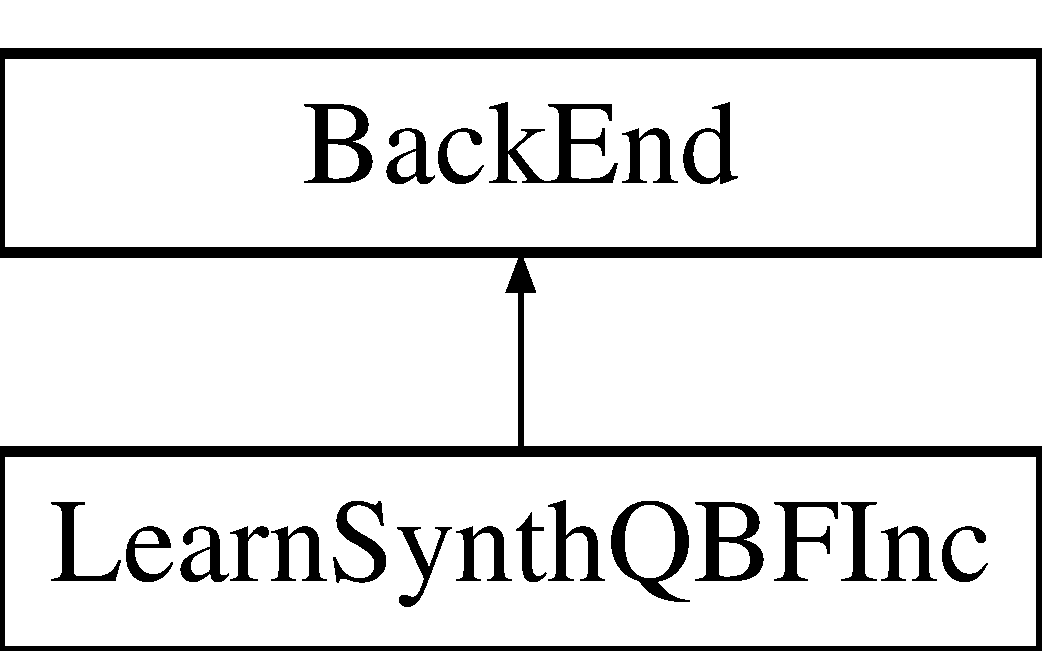
\includegraphics[height=2.000000cm]{classLearnSynthQBFInc}
\end{center}
\end{figure}
\subsection*{Public Member Functions}
\begin{DoxyCompactItemize}
\item 
\hyperlink{classLearnSynthQBFInc_a85d45b72b949faaa910d7a7569cc4877}{Learn\-Synth\-Q\-B\-F\-Inc} ()
\begin{DoxyCompactList}\small\item\em Constructor. \end{DoxyCompactList}\item 
virtual \hyperlink{classLearnSynthQBFInc_a9d9e0b1d3aa1ea85da6884af34cdc003}{$\sim$\-Learn\-Synth\-Q\-B\-F\-Inc} ()
\begin{DoxyCompactList}\small\item\em Destructor. \end{DoxyCompactList}\item 
virtual bool \hyperlink{classLearnSynthQBFInc_af9563d1f3c657ed4730ee49e041bc300}{run} ()
\begin{DoxyCompactList}\small\item\em Executes this back-\/end. \end{DoxyCompactList}\end{DoxyCompactItemize}
\subsection*{Protected Member Functions}
\begin{DoxyCompactItemize}
\item 
bool \hyperlink{classLearnSynthQBFInc_a2dc9fff9a414a40059a1d89e19b48252}{compute\-Winning\-Region} ()
\begin{DoxyCompactList}\small\item\em Computes the winning region and stores the result in \hyperlink{classLearnSynthQBFInc_abc3503bdb6be7053a7c3d3d7e57858d6}{winning\-\_\-region\-\_\-}. \end{DoxyCompactList}\item 
bool \hyperlink{classLearnSynthQBFInc_ab1090850d850dfcc0dacbf43426910ca}{compute\-Winning\-Region\-One} ()
\begin{DoxyCompactList}\small\item\em Uses the standard method to compute the winning region, with incremental solving. \end{DoxyCompactList}\item 
bool \hyperlink{classLearnSynthQBFInc_a796673a80bbba7c8b4b7b5b9e4c8332a}{compute\-Winning\-Region\-All} ()
\begin{DoxyCompactList}\small\item\em Computes the winning region, always computing all counterexample generalizations. \end{DoxyCompactList}\item 
bool \hyperlink{classLearnSynthQBFInc_ac30a0ff65a78a651d7760c4802485355}{compute\-Counterexample\-Q\-B\-F} (vector$<$ int $>$ \&ce)
\begin{DoxyCompactList}\small\item\em Computes a counterexample-\/state using a Q\-B\-F-\/solver with incremental solving. \end{DoxyCompactList}\item 
bool \hyperlink{classLearnSynthQBFInc_a52cfd07ff4d94cb9f42eed732ca166dd}{compute\-Blocking\-Clause} (vector$<$ int $>$ \&ce, vector$<$ int $>$ \&blocking\-\_\-clause)
\begin{DoxyCompactList}\small\item\em Computes a blocking clause for a counterexample. \end{DoxyCompactList}\item 
bool \hyperlink{classLearnSynthQBFInc_a979ac9b4cb4d6a8017da2a5e2ba97c82}{compute\-All\-Blocking\-Clauses} (vector$<$ int $>$ \&ce, vector$<$ vector$<$ int $>$ $>$ \&blocking\-\_\-clauses)
\begin{DoxyCompactList}\small\item\em Computes all minimal blocking clauses for a counterexample. \end{DoxyCompactList}\item 
void \hyperlink{classLearnSynthQBFInc_a492a35b7aa57af25fe47b0693f4ec14c}{reduce\-Existing\-Clauses} ()
\begin{DoxyCompactList}\small\item\em Tries to drop literals from clauses in the winning region. \end{DoxyCompactList}\item 
void \hyperlink{classLearnSynthQBFInc_a9493b7c067234879ce68ba73cf510b59}{recompute\-Check\-C\-N\-F} (bool take\-\_\-small\-\_\-win=true)
\begin{DoxyCompactList}\small\item\em Recomputes the \hyperlink{classCNF}{C\-N\-F} (of the Q\-B\-F) that is used for computing counterexamples. \end{DoxyCompactList}\item 
void \hyperlink{classLearnSynthQBFInc_a98fa456db980f739d6825e1ee6c96cfa}{recompute\-Gen\-C\-N\-F} (bool take\-\_\-small\-\_\-win=true)
\begin{DoxyCompactList}\small\item\em Recomputes the \hyperlink{classCNF}{C\-N\-F} (of the Q\-B\-F) that is used for generalizing counterexamples. \end{DoxyCompactList}\item 
void \hyperlink{classLearnSynthQBFInc_acefbf03dca5bf13532c6fc3209a21e69}{restrict\-To\-States} (vector$<$ int $>$ \&vec) const 
\begin{DoxyCompactList}\small\item\em Restricts a vector of literals (a cube or clause) to state-\/variables only. \end{DoxyCompactList}\item 
bool \hyperlink{classLearnSynthQBFInc_a01b407cc989eae78f6f3e5c607a91dd5}{generalize\-Counterexample} (vector$<$ int $>$ \&ce)
\begin{DoxyCompactList}\small\item\em Generalizes a counterexample-\/state by dropping literals. \end{DoxyCompactList}\end{DoxyCompactItemize}
\subsection*{Protected Attributes}
\begin{DoxyCompactItemize}
\item 
\hyperlink{classCNF}{C\-N\-F} \hyperlink{classLearnSynthQBFInc_abc3503bdb6be7053a7c3d3d7e57858d6}{winning\-\_\-region\-\_\-}
\begin{DoxyCompactList}\small\item\em The current over-\/approximation of the winning region. \end{DoxyCompactList}\item 
\hyperlink{classCNF}{C\-N\-F} \hyperlink{classLearnSynthQBFInc_a5ef45d9d77b566fca1c5a1e6041f7c86}{winning\-\_\-region\-\_\-large\-\_\-}
\begin{DoxyCompactList}\small\item\em The current over-\/approximation of the winning region in an uncompressed form. \end{DoxyCompactList}\item 
\hyperlink{classLearnStatisticsQBF}{Learn\-Statistics\-Q\-B\-F} \hyperlink{classLearnSynthQBFInc_a1f8d3bd97419754ef72759bdda766db4}{statistics\-\_\-}
\begin{DoxyCompactList}\small\item\em Stores and maintains statistics and performance measures. \end{DoxyCompactList}\item 
vector$<$ pair$<$ \hyperlink{classVarInfo_a64d1da76cf84fe674e5fef9764ef11cf}{Var\-Info\-::\-Var\-Kind}, \\*
\hyperlink{classQBFSolver_ac091e263cb55286cc07b2451bcf4d3c7}{Q\-B\-F\-Solver\-::\-Quant} $>$ $>$ \hyperlink{classLearnSynthQBFInc_a1430ac66d026f9e3f30619082f378426}{check\-\_\-quant\-\_\-}
\begin{DoxyCompactList}\small\item\em The quantifier prefix of the Q\-B\-F for computing counterexamples. \end{DoxyCompactList}\item 
\hyperlink{classCNF}{C\-N\-F} \hyperlink{classLearnSynthQBFInc_ac0ab1f2bc45740dc3e3e28e04a98d62d}{check\-\_\-cnf\-\_\-}
\begin{DoxyCompactList}\small\item\em The \hyperlink{classCNF}{C\-N\-F} matrix of the Q\-B\-F for computing counterexamples. \end{DoxyCompactList}\item 
\hyperlink{classDepQBFApiInc}{Dep\-Q\-B\-F\-Api\-Inc} \hyperlink{classLearnSynthQBFInc_aff50a974e8faf0e9e9d7431b46e0d8c5}{solver\-\_\-check\-\_\-}
\begin{DoxyCompactList}\small\item\em The Q\-B\-F-\/solver used for computing counterexamples. \end{DoxyCompactList}\item 
vector$<$ pair$<$ \hyperlink{classVarInfo_a64d1da76cf84fe674e5fef9764ef11cf}{Var\-Info\-::\-Var\-Kind}, \\*
\hyperlink{classQBFSolver_ac091e263cb55286cc07b2451bcf4d3c7}{Q\-B\-F\-Solver\-::\-Quant} $>$ $>$ \hyperlink{classLearnSynthQBFInc_af42c16902cfccdf51d1c1bc112be0ee4}{gen\-\_\-quant\-\_\-}
\begin{DoxyCompactList}\small\item\em The quantifier prefix of the Q\-B\-F for generalizing counterexamples. \end{DoxyCompactList}\item 
\hyperlink{classCNF}{C\-N\-F} \hyperlink{classLearnSynthQBFInc_ad3d20b7d5e6b561c7cf46324962247ba}{generalize\-\_\-clause\-\_\-cnf\-\_\-}
\begin{DoxyCompactList}\small\item\em The \hyperlink{classCNF}{C\-N\-F} matrix of the Q\-B\-F for generalizing counterexamples. \end{DoxyCompactList}\item 
\hyperlink{classDepQBFApiInc}{Dep\-Q\-B\-F\-Api\-Inc} \hyperlink{classLearnSynthQBFInc_a8cb5e0c1c5516ac1d65537c64794ec0a}{solver\-\_\-gen\-\_\-}
\begin{DoxyCompactList}\small\item\em The Q\-B\-F-\/solver used for generalizing counterexamples. \end{DoxyCompactList}\end{DoxyCompactItemize}
\subsection*{Private Member Functions}
\begin{DoxyCompactItemize}
\item 
\hyperlink{classLearnSynthQBFInc_adbb7481fd8c287942417c9ae75b06e8b}{Learn\-Synth\-Q\-B\-F\-Inc} (const \hyperlink{classLearnSynthQBFInc}{Learn\-Synth\-Q\-B\-F\-Inc} \&other)
\begin{DoxyCompactList}\small\item\em Copy constructor. \end{DoxyCompactList}\item 
\hyperlink{classLearnSynthQBFInc}{Learn\-Synth\-Q\-B\-F\-Inc} \& \hyperlink{classLearnSynthQBFInc_a09bc59c4c8a80e064fe4535314ee2acb}{operator=} (const \hyperlink{classLearnSynthQBFInc}{Learn\-Synth\-Q\-B\-F\-Inc} \&other)
\begin{DoxyCompactList}\small\item\em Assignment operator. \end{DoxyCompactList}\end{DoxyCompactItemize}


\subsection{Detailed Description}
Implements a learning-\/based synthesis with incremental Q\-B\-F solving. 

This class is almost an exact copy of \hyperlink{classLearnSynthQBF}{Learn\-Synth\-Q\-B\-F}. Hence, we refer to the documentation of \hyperlink{classLearnSynthQBF}{Learn\-Synth\-Q\-B\-F} for an explanation of the basic working principle. The main difference is that this class utilizes features which are only available in an experimental version of the Dep\-Q\-B\-F Q\-B\-F-\/solver (see \hyperlink{classDepQBFApiInc}{Dep\-Q\-B\-F\-Api\-Inc}). The additional features of \hyperlink{classDepQBFApiInc}{Dep\-Q\-B\-F\-Api\-Inc} are the computation of unsatisfiable cores and a restricted way of incremental solving. 'Restricted' means\-: we can (only) add new clauses that talk only about variables that are quantified existentially on the outermost level to the solver without restarting it completely. This way the solver can keep all the clauses it learned so far.

\begin{DoxyNote}{Note}
This class is experimental. 
\end{DoxyNote}
\begin{DoxyAuthor}{Author}
Robert Koenighofer (\href{mailto:robert.koenighofer@iaik.tugraz.at}{\tt robert.\-koenighofer@iaik.\-tugraz.\-at}) 
\end{DoxyAuthor}
\begin{DoxyVersion}{Version}
1.\-0.\-0 
\end{DoxyVersion}


Definition at line 60 of file Learn\-Synth\-Q\-B\-F\-Inc.\-h.



\subsection{Constructor \& Destructor Documentation}
\hypertarget{classLearnSynthQBFInc_a85d45b72b949faaa910d7a7569cc4877}{\index{Learn\-Synth\-Q\-B\-F\-Inc@{Learn\-Synth\-Q\-B\-F\-Inc}!Learn\-Synth\-Q\-B\-F\-Inc@{Learn\-Synth\-Q\-B\-F\-Inc}}
\index{Learn\-Synth\-Q\-B\-F\-Inc@{Learn\-Synth\-Q\-B\-F\-Inc}!LearnSynthQBFInc@{Learn\-Synth\-Q\-B\-F\-Inc}}
\subsubsection[{Learn\-Synth\-Q\-B\-F\-Inc}]{\setlength{\rightskip}{0pt plus 5cm}Learn\-Synth\-Q\-B\-F\-Inc\-::\-Learn\-Synth\-Q\-B\-F\-Inc (
\begin{DoxyParamCaption}
{}
\end{DoxyParamCaption}
)}}\label{classLearnSynthQBFInc_a85d45b72b949faaa910d7a7569cc4877}


Constructor. 



Definition at line 40 of file Learn\-Synth\-Q\-B\-F\-Inc.\-cpp.



References Q\-B\-F\-Solver\-::\-A, check\-\_\-quant\-\_\-, Var\-Info\-::\-C\-T\-R\-L, Q\-B\-F\-Solver\-::\-E, gen\-\_\-quant\-\_\-, Var\-Info\-::\-I\-N\-P\-U\-T, Var\-Info\-::\-N\-E\-X\-T\-\_\-\-S\-T\-A\-T\-E, Var\-Info\-::\-P\-R\-E\-S\-\_\-\-S\-T\-A\-T\-E, and Var\-Info\-::\-T\-M\-P.

\hypertarget{classLearnSynthQBFInc_a9d9e0b1d3aa1ea85da6884af34cdc003}{\index{Learn\-Synth\-Q\-B\-F\-Inc@{Learn\-Synth\-Q\-B\-F\-Inc}!$\sim$\-Learn\-Synth\-Q\-B\-F\-Inc@{$\sim$\-Learn\-Synth\-Q\-B\-F\-Inc}}
\index{$\sim$\-Learn\-Synth\-Q\-B\-F\-Inc@{$\sim$\-Learn\-Synth\-Q\-B\-F\-Inc}!LearnSynthQBFInc@{Learn\-Synth\-Q\-B\-F\-Inc}}
\subsubsection[{$\sim$\-Learn\-Synth\-Q\-B\-F\-Inc}]{\setlength{\rightskip}{0pt plus 5cm}Learn\-Synth\-Q\-B\-F\-Inc\-::$\sim$\-Learn\-Synth\-Q\-B\-F\-Inc (
\begin{DoxyParamCaption}
{}
\end{DoxyParamCaption}
)\hspace{0.3cm}{\ttfamily [virtual]}}}\label{classLearnSynthQBFInc_a9d9e0b1d3aa1ea85da6884af34cdc003}


Destructor. 



Definition at line 63 of file Learn\-Synth\-Q\-B\-F\-Inc.\-cpp.

\hypertarget{classLearnSynthQBFInc_adbb7481fd8c287942417c9ae75b06e8b}{\index{Learn\-Synth\-Q\-B\-F\-Inc@{Learn\-Synth\-Q\-B\-F\-Inc}!Learn\-Synth\-Q\-B\-F\-Inc@{Learn\-Synth\-Q\-B\-F\-Inc}}
\index{Learn\-Synth\-Q\-B\-F\-Inc@{Learn\-Synth\-Q\-B\-F\-Inc}!LearnSynthQBFInc@{Learn\-Synth\-Q\-B\-F\-Inc}}
\subsubsection[{Learn\-Synth\-Q\-B\-F\-Inc}]{\setlength{\rightskip}{0pt plus 5cm}Learn\-Synth\-Q\-B\-F\-Inc\-::\-Learn\-Synth\-Q\-B\-F\-Inc (
\begin{DoxyParamCaption}
\item[{const {\bf Learn\-Synth\-Q\-B\-F\-Inc} \&}]{other}
\end{DoxyParamCaption}
)\hspace{0.3cm}{\ttfamily [private]}}}\label{classLearnSynthQBFInc_adbb7481fd8c287942417c9ae75b06e8b}


Copy constructor. 

The copy constructor is disabled (set private) and not implemented.


\begin{DoxyParams}{Parameters}
{\em other} & The source for creating the copy. \\
\hline
\end{DoxyParams}


\subsection{Member Function Documentation}
\hypertarget{classLearnSynthQBFInc_a979ac9b4cb4d6a8017da2a5e2ba97c82}{\index{Learn\-Synth\-Q\-B\-F\-Inc@{Learn\-Synth\-Q\-B\-F\-Inc}!compute\-All\-Blocking\-Clauses@{compute\-All\-Blocking\-Clauses}}
\index{compute\-All\-Blocking\-Clauses@{compute\-All\-Blocking\-Clauses}!LearnSynthQBFInc@{Learn\-Synth\-Q\-B\-F\-Inc}}
\subsubsection[{compute\-All\-Blocking\-Clauses}]{\setlength{\rightskip}{0pt plus 5cm}bool Learn\-Synth\-Q\-B\-F\-Inc\-::compute\-All\-Blocking\-Clauses (
\begin{DoxyParamCaption}
\item[{vector$<$ int $>$ \&}]{ce, }
\item[{vector$<$ vector$<$ int $>$ $>$ \&}]{blocking\-\_\-clauses}
\end{DoxyParamCaption}
)\hspace{0.3cm}{\ttfamily [protected]}}}\label{classLearnSynthQBFInc_a979ac9b4cb4d6a8017da2a5e2ba97c82}


Computes all minimal blocking clauses for a counterexample. 

This method works like \hyperlink{classLearnSynthQBF_affa7b4583cc17d01f4c82fd57e763e1f}{Learn\-Synth\-Q\-B\-F\-::compute\-All\-Blocking\-Clauses()} but using unsatisfiable cores to generalize the counterexample instead of just iterating over the literals.


\begin{DoxyParams}{Parameters}
{\em ce} & The counterexample to block. It is a full or partial cube over the state variables. \\
\hline
{\em blocking\-\_\-clauses} & An empty vector. It is used to store the computed blocking clauses. The counterexample falsifies all blocking clauses in this vector. \\
\hline
\end{DoxyParams}
\begin{DoxyReturn}{Returns}
False if one of the blocking clauses blocks the initial state. This means that the initial state is removed from the winning region, i.\-e., the specification is unrealizable. True is returned otherwise. 
\end{DoxyReturn}


Definition at line 321 of file Learn\-Synth\-Q\-B\-F\-Inc.\-cpp.



References C\-N\-F\-::add\-Clause(), Utils\-::contains\-Init(), gen\-\_\-quant\-\_\-, generalize\-\_\-clause\-\_\-cnf\-\_\-, generalize\-Counterexample(), Dep\-Q\-B\-F\-Api\-Inc\-::inc\-Add\-C\-N\-F(), Utils\-::intersection\-Empty(), Utils\-::negate\-Literals(), Learn\-Statistics\-Q\-B\-F\-::notify\-After\-Cube\-Min(), Learn\-Statistics\-Q\-B\-F\-::notify\-Before\-Cube\-Min(), Learn\-Statistics\-Q\-B\-F\-::notify\-Cube\-Min(), Utils\-::remove(), solver\-\_\-gen\-\_\-, Dep\-Q\-B\-F\-Api\-Inc\-::start\-Incremental\-Session(), statistics\-\_\-, and Utils\-::swap\-Present\-To\-Next().



Referenced by compute\-Winning\-Region\-All().

\hypertarget{classLearnSynthQBFInc_a52cfd07ff4d94cb9f42eed732ca166dd}{\index{Learn\-Synth\-Q\-B\-F\-Inc@{Learn\-Synth\-Q\-B\-F\-Inc}!compute\-Blocking\-Clause@{compute\-Blocking\-Clause}}
\index{compute\-Blocking\-Clause@{compute\-Blocking\-Clause}!LearnSynthQBFInc@{Learn\-Synth\-Q\-B\-F\-Inc}}
\subsubsection[{compute\-Blocking\-Clause}]{\setlength{\rightskip}{0pt plus 5cm}bool Learn\-Synth\-Q\-B\-F\-Inc\-::compute\-Blocking\-Clause (
\begin{DoxyParamCaption}
\item[{vector$<$ int $>$ \&}]{ce, }
\item[{vector$<$ int $>$ \&}]{blocking\-\_\-clause}
\end{DoxyParamCaption}
)\hspace{0.3cm}{\ttfamily [protected]}}}\label{classLearnSynthQBFInc_a52cfd07ff4d94cb9f42eed732ca166dd}


Computes a blocking clause for a counterexample. 

This method works like \hyperlink{classLearnSynthQBF_a73856a79be3fb7e260485bcda7c31f80}{Learn\-Synth\-Q\-B\-F\-::compute\-Blocking\-Clause()} but using unsatisfiable cores to generalize the counterexample instead of just iterating over the literals.


\begin{DoxyParams}{Parameters}
{\em ce} & The counterexample to block. It is a full or partial cube over the state variables. \\
\hline
{\em blocking\-\_\-clause} & An empty vector. It is used to store the computed blocking clause. The counterexample falsifies the blocking clause. \\
\hline
\end{DoxyParams}
\begin{DoxyReturn}{Returns}
False if the blocking clause blocks the initial state. This means that the initial state is removed from the winning region, i.\-e., the specification is unrealizable. True is returned otherwise. 
\end{DoxyReturn}


Definition at line 289 of file Learn\-Synth\-Q\-B\-F\-Inc.\-cpp.



References C\-N\-F\-::add\-Clause(), Utils\-::contains\-Init(), gen\-\_\-quant\-\_\-, generalize\-\_\-clause\-\_\-cnf\-\_\-, generalize\-Counterexample(), Dep\-Q\-B\-F\-Api\-Inc\-::inc\-Add\-C\-N\-F(), L\-\_\-\-D\-B\-G, Utils\-::negate\-Literals(), Learn\-Statistics\-Q\-B\-F\-::notify\-After\-Cube\-Min(), Learn\-Statistics\-Q\-B\-F\-::notify\-Before\-Cube\-Min(), Utils\-::randomize(), solver\-\_\-gen\-\_\-, Dep\-Q\-B\-F\-Api\-Inc\-::start\-Incremental\-Session(), statistics\-\_\-, and Utils\-::swap\-Present\-To\-Next().



Referenced by compute\-Winning\-Region\-One().

\hypertarget{classLearnSynthQBFInc_ac30a0ff65a78a651d7760c4802485355}{\index{Learn\-Synth\-Q\-B\-F\-Inc@{Learn\-Synth\-Q\-B\-F\-Inc}!compute\-Counterexample\-Q\-B\-F@{compute\-Counterexample\-Q\-B\-F}}
\index{compute\-Counterexample\-Q\-B\-F@{compute\-Counterexample\-Q\-B\-F}!LearnSynthQBFInc@{Learn\-Synth\-Q\-B\-F\-Inc}}
\subsubsection[{compute\-Counterexample\-Q\-B\-F}]{\setlength{\rightskip}{0pt plus 5cm}bool Learn\-Synth\-Q\-B\-F\-Inc\-::compute\-Counterexample\-Q\-B\-F (
\begin{DoxyParamCaption}
\item[{vector$<$ int $>$ \&}]{ce}
\end{DoxyParamCaption}
)\hspace{0.3cm}{\ttfamily [protected]}}}\label{classLearnSynthQBFInc_ac30a0ff65a78a651d7760c4802485355}


Computes a counterexample-\/state using a Q\-B\-F-\/solver with incremental solving. 

This method works like \hyperlink{classLearnSynthQBF_a04b8dd6e26d646a6f197afb362168408}{Learn\-Synth\-Q\-B\-F\-::compute\-Counterexample\-Q\-B\-F()} but using incremental solving and unsatisfiable cores. 'Using incremental solving' means, instead of solving exists x,i\-: forall c\-: exists x',tmp\-: F \& T \& !\-F' where F is the \hyperlink{classLearnSynthQBFInc_abc3503bdb6be7053a7c3d3d7e57858d6}{winning\-\_\-region\-\_\-} we solve exists x,i\-: forall c\-: exists x',tmp\-: F \& T \& !\-G' where G is a copy of F that is updated only lazily. That is, whenever new clauses are discovered, they are added only to F but not to G. Only if this method returns false, we update G \-:= F and try again. The synthesis algorithm only aborts if false is returned while G = F.


\begin{DoxyParams}{Parameters}
{\em ce} & An empty vector. The computed counterexample is stored in this vector in form of a cube over the state variables. The cube does not necessarily contain all state variables. If some state variables are irrelevant, then they may be omitted. \\
\hline
\end{DoxyParams}
\begin{DoxyReturn}{Returns}
True if a counterexample was found, false if no counterexample exists. 
\end{DoxyReturn}


Definition at line 277 of file Learn\-Synth\-Q\-B\-F\-Inc.\-cpp.



References Dep\-Q\-B\-F\-Api\-Inc\-::inc\-Is\-Sat\-Model\-Or\-Core(), Learn\-Statistics\-Q\-B\-F\-::notify\-After\-Compute\-Cube(), Learn\-Statistics\-Q\-B\-F\-::notify\-Before\-Compute\-Cube(), restrict\-To\-States(), solver\-\_\-check\-\_\-, and statistics\-\_\-.



Referenced by compute\-Winning\-Region\-All(), and compute\-Winning\-Region\-One().

\hypertarget{classLearnSynthQBFInc_a2dc9fff9a414a40059a1d89e19b48252}{\index{Learn\-Synth\-Q\-B\-F\-Inc@{Learn\-Synth\-Q\-B\-F\-Inc}!compute\-Winning\-Region@{compute\-Winning\-Region}}
\index{compute\-Winning\-Region@{compute\-Winning\-Region}!LearnSynthQBFInc@{Learn\-Synth\-Q\-B\-F\-Inc}}
\subsubsection[{compute\-Winning\-Region}]{\setlength{\rightskip}{0pt plus 5cm}bool Learn\-Synth\-Q\-B\-F\-Inc\-::compute\-Winning\-Region (
\begin{DoxyParamCaption}
{}
\end{DoxyParamCaption}
)\hspace{0.3cm}{\ttfamily [protected]}}}\label{classLearnSynthQBFInc_a2dc9fff9a414a40059a1d89e19b48252}


Computes the winning region and stores the result in \hyperlink{classLearnSynthQBFInc_abc3503bdb6be7053a7c3d3d7e57858d6}{winning\-\_\-region\-\_\-}. 

Depending on the command-\/line parameters (--mode) this method calls one of 
\begin{DoxyItemize}
\item \hyperlink{classLearnSynthQBFInc_ab1090850d850dfcc0dacbf43426910ca}{compute\-Winning\-Region\-One()} 
\item \hyperlink{classLearnSynthQBFInc_a796673a80bbba7c8b4b7b5b9e4c8332a}{compute\-Winning\-Region\-All()} 
\end{DoxyItemize}

\begin{DoxyReturn}{Returns}
True if the specification was realizable, false otherwise. 
\end{DoxyReturn}


Definition at line 104 of file Learn\-Synth\-Q\-B\-F\-Inc.\-cpp.



References compute\-Winning\-Region\-All(), compute\-Winning\-Region\-One(), and Options\-::instance().



Referenced by run().

\hypertarget{classLearnSynthQBFInc_a796673a80bbba7c8b4b7b5b9e4c8332a}{\index{Learn\-Synth\-Q\-B\-F\-Inc@{Learn\-Synth\-Q\-B\-F\-Inc}!compute\-Winning\-Region\-All@{compute\-Winning\-Region\-All}}
\index{compute\-Winning\-Region\-All@{compute\-Winning\-Region\-All}!LearnSynthQBFInc@{Learn\-Synth\-Q\-B\-F\-Inc}}
\subsubsection[{compute\-Winning\-Region\-All}]{\setlength{\rightskip}{0pt plus 5cm}bool Learn\-Synth\-Q\-B\-F\-Inc\-::compute\-Winning\-Region\-All (
\begin{DoxyParamCaption}
{}
\end{DoxyParamCaption}
)\hspace{0.3cm}{\ttfamily [protected]}}}\label{classLearnSynthQBFInc_a796673a80bbba7c8b4b7b5b9e4c8332a}


Computes the winning region, always computing all counterexample generalizations. 

This method works like \hyperlink{classLearnSynthQBF_a09a9ecb2b77c540cdcc327a35cd15c18}{Learn\-Synth\-Q\-B\-F\-::compute\-Winning\-Region\-All()} but using incremental solving and unsatisfiable cores.

\begin{DoxyReturn}{Returns}
True if the specification was realizable, false otherwise. 
\end{DoxyReturn}


Definition at line 192 of file Learn\-Synth\-Q\-B\-F\-Inc.\-cpp.



References C\-N\-F\-::add\-Clause\-And\-Simplify(), check\-\_\-cnf\-\_\-, check\-\_\-quant\-\_\-, C\-N\-F\-::clear(), Utils\-::compress\-State\-C\-N\-F(), compute\-All\-Blocking\-Clauses(), compute\-Counterexample\-Q\-B\-F(), Var\-Info\-::\-C\-T\-R\-L, Logger\-::\-D\-B\-G, Utils\-::debug\-Print(), gen\-\_\-quant\-\_\-, generalize\-\_\-clause\-\_\-cnf\-\_\-, C\-N\-F\-::get\-Nr\-Of\-Clauses(), C\-N\-F\-::get\-Nr\-Of\-Lits(), A\-I\-G2\-C\-N\-F\-::get\-Safe\-States(), Var\-Manager\-::get\-Vars\-Of\-Type(), Dep\-Q\-B\-F\-Api\-Inc\-::inc\-Add\-Clause(), Dep\-Q\-B\-F\-Api\-Inc\-::inc\-Add\-C\-N\-F(), Var\-Info\-::\-I\-N\-P\-U\-T, Var\-Manager\-::instance(), Logger\-::instance(), A\-I\-G2\-C\-N\-F\-::instance(), Logger\-::is\-Enabled(), L\-\_\-\-D\-B\-G, Learn\-Statistics\-Q\-B\-F\-::log\-Statistics(), Var\-Info\-::\-P\-R\-E\-S\-\_\-\-S\-T\-A\-T\-E, recompute\-Check\-C\-N\-F(), recompute\-Gen\-C\-N\-F(), reduce\-Existing\-Clauses(), solver\-\_\-check\-\_\-, solver\-\_\-gen\-\_\-, Dep\-Q\-B\-F\-Api\-Inc\-::start\-Incremental\-Session(), statistics\-\_\-, winning\-\_\-region\-\_\-, and winning\-\_\-region\-\_\-large\-\_\-.



Referenced by compute\-Winning\-Region().

\hypertarget{classLearnSynthQBFInc_ab1090850d850dfcc0dacbf43426910ca}{\index{Learn\-Synth\-Q\-B\-F\-Inc@{Learn\-Synth\-Q\-B\-F\-Inc}!compute\-Winning\-Region\-One@{compute\-Winning\-Region\-One}}
\index{compute\-Winning\-Region\-One@{compute\-Winning\-Region\-One}!LearnSynthQBFInc@{Learn\-Synth\-Q\-B\-F\-Inc}}
\subsubsection[{compute\-Winning\-Region\-One}]{\setlength{\rightskip}{0pt plus 5cm}bool Learn\-Synth\-Q\-B\-F\-Inc\-::compute\-Winning\-Region\-One (
\begin{DoxyParamCaption}
{}
\end{DoxyParamCaption}
)\hspace{0.3cm}{\ttfamily [protected]}}}\label{classLearnSynthQBFInc_ab1090850d850dfcc0dacbf43426910ca}


Uses the standard method to compute the winning region, with incremental solving. 

This method works like \hyperlink{classLearnSynthQBF_ac538cd53082bad1c8c45a7e178dfa4cb}{Learn\-Synth\-Q\-B\-F\-::compute\-Winning\-Region\-One()} but using incremental solving and unsatisfiable cores.

\begin{DoxyReturn}{Returns}
True if the specification was realizable, false otherwise. 
\end{DoxyReturn}


Definition at line 112 of file Learn\-Synth\-Q\-B\-F\-Inc.\-cpp.



References C\-N\-F\-::add\-Clause\-And\-Simplify(), check\-\_\-cnf\-\_\-, check\-\_\-quant\-\_\-, C\-N\-F\-::clear(), Utils\-::compress\-State\-C\-N\-F(), compute\-Blocking\-Clause(), compute\-Counterexample\-Q\-B\-F(), Var\-Info\-::\-C\-T\-R\-L, Logger\-::\-D\-B\-G, Utils\-::debug\-Print(), gen\-\_\-quant\-\_\-, generalize\-\_\-clause\-\_\-cnf\-\_\-, C\-N\-F\-::get\-Nr\-Of\-Clauses(), C\-N\-F\-::get\-Nr\-Of\-Lits(), A\-I\-G2\-C\-N\-F\-::get\-Safe\-States(), Var\-Manager\-::get\-Vars\-Of\-Type(), Dep\-Q\-B\-F\-Api\-Inc\-::inc\-Add\-Clause(), Dep\-Q\-B\-F\-Api\-Inc\-::inc\-Add\-C\-N\-F(), Var\-Info\-::\-I\-N\-P\-U\-T, Var\-Manager\-::instance(), Logger\-::instance(), A\-I\-G2\-C\-N\-F\-::instance(), Logger\-::is\-Enabled(), L\-\_\-\-D\-B\-G, Learn\-Statistics\-Q\-B\-F\-::log\-Statistics(), Var\-Info\-::\-P\-R\-E\-S\-\_\-\-S\-T\-A\-T\-E, recompute\-Check\-C\-N\-F(), recompute\-Gen\-C\-N\-F(), solver\-\_\-check\-\_\-, solver\-\_\-gen\-\_\-, Dep\-Q\-B\-F\-Api\-Inc\-::start\-Incremental\-Session(), statistics\-\_\-, winning\-\_\-region\-\_\-, and winning\-\_\-region\-\_\-large\-\_\-.



Referenced by compute\-Winning\-Region().

\hypertarget{classLearnSynthQBFInc_a01b407cc989eae78f6f3e5c607a91dd5}{\index{Learn\-Synth\-Q\-B\-F\-Inc@{Learn\-Synth\-Q\-B\-F\-Inc}!generalize\-Counterexample@{generalize\-Counterexample}}
\index{generalize\-Counterexample@{generalize\-Counterexample}!LearnSynthQBFInc@{Learn\-Synth\-Q\-B\-F\-Inc}}
\subsubsection[{generalize\-Counterexample}]{\setlength{\rightskip}{0pt plus 5cm}bool Learn\-Synth\-Q\-B\-F\-Inc\-::generalize\-Counterexample (
\begin{DoxyParamCaption}
\item[{vector$<$ int $>$ \&}]{ce}
\end{DoxyParamCaption}
)\hspace{0.3cm}{\ttfamily [protected]}}}\label{classLearnSynthQBFInc_a01b407cc989eae78f6f3e5c607a91dd5}


Generalizes a counterexample-\/state by dropping literals. 

This method works like \hyperlink{classLearnSynthQBF_a9eed607741968f74e31976e8ca40a62f}{Learn\-Synth\-Q\-B\-F\-::generalize\-Counterexample()} but using unsatisfiable cores to generalize the counterexample instead of just iterating over the literals.


\begin{DoxyParams}{Parameters}
{\em ce} & The counterexample to generalize (it will be overwritten by its own generalization). This is a complete or partial cube over the present state variables. \\
\hline
\end{DoxyParams}
\begin{DoxyReturn}{Returns}
True if the passed vector is a valid (generalization of a) counterexample, false otherwise. 
\end{DoxyReturn}


Definition at line 521 of file Learn\-Synth\-Q\-B\-F\-Inc.\-cpp.



References Dep\-Q\-B\-F\-Api\-Inc\-::inc\-Is\-Sat\-Model\-Or\-Core(), solver\-\_\-gen\-\_\-, and Utils\-::sort().



Referenced by compute\-All\-Blocking\-Clauses(), compute\-Blocking\-Clause(), and reduce\-Existing\-Clauses().

\hypertarget{classLearnSynthQBFInc_a09bc59c4c8a80e064fe4535314ee2acb}{\index{Learn\-Synth\-Q\-B\-F\-Inc@{Learn\-Synth\-Q\-B\-F\-Inc}!operator=@{operator=}}
\index{operator=@{operator=}!LearnSynthQBFInc@{Learn\-Synth\-Q\-B\-F\-Inc}}
\subsubsection[{operator=}]{\setlength{\rightskip}{0pt plus 5cm}{\bf Learn\-Synth\-Q\-B\-F\-Inc}\& Learn\-Synth\-Q\-B\-F\-Inc\-::operator= (
\begin{DoxyParamCaption}
\item[{const {\bf Learn\-Synth\-Q\-B\-F\-Inc} \&}]{other}
\end{DoxyParamCaption}
)\hspace{0.3cm}{\ttfamily [private]}}}\label{classLearnSynthQBFInc_a09bc59c4c8a80e064fe4535314ee2acb}


Assignment operator. 

The assignment operator is disabled (set private) and not implemented.


\begin{DoxyParams}{Parameters}
{\em other} & The source for creating the copy. \\
\hline
\end{DoxyParams}
\begin{DoxyReturn}{Returns}
The result of the assignment, i.\-e, $\ast$this. 
\end{DoxyReturn}
\hypertarget{classLearnSynthQBFInc_a9493b7c067234879ce68ba73cf510b59}{\index{Learn\-Synth\-Q\-B\-F\-Inc@{Learn\-Synth\-Q\-B\-F\-Inc}!recompute\-Check\-C\-N\-F@{recompute\-Check\-C\-N\-F}}
\index{recompute\-Check\-C\-N\-F@{recompute\-Check\-C\-N\-F}!LearnSynthQBFInc@{Learn\-Synth\-Q\-B\-F\-Inc}}
\subsubsection[{recompute\-Check\-C\-N\-F}]{\setlength{\rightskip}{0pt plus 5cm}void Learn\-Synth\-Q\-B\-F\-Inc\-::recompute\-Check\-C\-N\-F (
\begin{DoxyParamCaption}
\item[{bool}]{take\-\_\-small\-\_\-win = {\ttfamily true}}
\end{DoxyParamCaption}
)\hspace{0.3cm}{\ttfamily [protected]}}}\label{classLearnSynthQBFInc_a9493b7c067234879ce68ba73cf510b59}


Recomputes the \hyperlink{classCNF}{C\-N\-F} (of the Q\-B\-F) that is used for computing counterexamples. 

The \hyperlink{classCNF}{C\-N\-F} used for computing counterexamples is F \& T \& !\-F', where F is the \hyperlink{classLearnSynthQBFInc_abc3503bdb6be7053a7c3d3d7e57858d6}{winning\-\_\-region\-\_\-}. The result is stored in \hyperlink{classLearnSynthQBFInc_ac0ab1f2bc45740dc3e3e28e04a98d62d}{check\-\_\-cnf\-\_\-}. In contrast to \hyperlink{classLearnSynthQBF}{Learn\-Synth\-Q\-B\-F}, this class calls this method not so often (only when \hyperlink{classLearnSynthQBFInc_ac30a0ff65a78a651d7760c4802485355}{compute\-Counterexample\-Q\-B\-F()} returns unsatisfiable.


\begin{DoxyParams}{Parameters}
{\em take\-\_\-small\-\_\-win} & If this parameter is true (or omitted) the \hyperlink{classLearnSynthQBFInc_abc3503bdb6be7053a7c3d3d7e57858d6}{winning\-\_\-region\-\_\-} is used to compute the \hyperlink{classLearnSynthQBFInc_ac0ab1f2bc45740dc3e3e28e04a98d62d}{check\-\_\-cnf\-\_\-}. Otherwise, the \hyperlink{classLearnSynthQBFInc_a5ef45d9d77b566fca1c5a1e6041f7c86}{winning\-\_\-region\-\_\-large\-\_\-} is used. The difference between these two winning region versions is as follows. From time to we remove redundant clauses (clauses implied by other clauses) from \hyperlink{classLearnSynthQBFInc_abc3503bdb6be7053a7c3d3d7e57858d6}{winning\-\_\-region\-\_\-} but not from \hyperlink{classLearnSynthQBFInc_a5ef45d9d77b566fca1c5a1e6041f7c86}{winning\-\_\-region\-\_\-large\-\_\-}. Hence, \hyperlink{classLearnSynthQBFInc_abc3503bdb6be7053a7c3d3d7e57858d6}{winning\-\_\-region\-\_\-} is often smaller, but \hyperlink{classLearnSynthQBFInc_a5ef45d9d77b566fca1c5a1e6041f7c86}{winning\-\_\-region\-\_\-large\-\_\-} may contain clauses the solver may have to learn when using \hyperlink{classLearnSynthQBFInc_abc3503bdb6be7053a7c3d3d7e57858d6}{winning\-\_\-region\-\_\-}. \\
\hline
\end{DoxyParams}


Definition at line 458 of file Learn\-Synth\-Q\-B\-F\-Inc.\-cpp.



References C\-N\-F\-::add\-C\-N\-F(), check\-\_\-cnf\-\_\-, C\-N\-F\-::clear(), A\-I\-G2\-C\-N\-F\-::instance(), C\-N\-F\-::negate(), Var\-Manager\-::reset\-To\-Last\-Push(), C\-N\-F\-::swap\-Present\-To\-Next(), winning\-\_\-region\-\_\-, and winning\-\_\-region\-\_\-large\-\_\-.



Referenced by compute\-Winning\-Region\-All(), and compute\-Winning\-Region\-One().

\hypertarget{classLearnSynthQBFInc_a98fa456db980f739d6825e1ee6c96cfa}{\index{Learn\-Synth\-Q\-B\-F\-Inc@{Learn\-Synth\-Q\-B\-F\-Inc}!recompute\-Gen\-C\-N\-F@{recompute\-Gen\-C\-N\-F}}
\index{recompute\-Gen\-C\-N\-F@{recompute\-Gen\-C\-N\-F}!LearnSynthQBFInc@{Learn\-Synth\-Q\-B\-F\-Inc}}
\subsubsection[{recompute\-Gen\-C\-N\-F}]{\setlength{\rightskip}{0pt plus 5cm}void Learn\-Synth\-Q\-B\-F\-Inc\-::recompute\-Gen\-C\-N\-F (
\begin{DoxyParamCaption}
\item[{bool}]{take\-\_\-small\-\_\-win = {\ttfamily true}}
\end{DoxyParamCaption}
)\hspace{0.3cm}{\ttfamily [protected]}}}\label{classLearnSynthQBFInc_a98fa456db980f739d6825e1ee6c96cfa}


Recomputes the \hyperlink{classCNF}{C\-N\-F} (of the Q\-B\-F) that is used for generalizing counterexamples. 

The \hyperlink{classCNF}{C\-N\-F} used for generalizing counterexamples is F \& T \& F', where F is the \hyperlink{classLearnSynthQBFInc_abc3503bdb6be7053a7c3d3d7e57858d6}{winning\-\_\-region\-\_\-}. The result is stored in \hyperlink{classLearnSynthQBFInc_ad3d20b7d5e6b561c7cf46324962247ba}{generalize\-\_\-clause\-\_\-cnf\-\_\-}. Since F is constantly updated with new clauses, \hyperlink{classLearnSynthQBFInc_ad3d20b7d5e6b561c7cf46324962247ba}{generalize\-\_\-clause\-\_\-cnf\-\_\-} needs to be updated as well. In an old version, we updated the \hyperlink{classLearnSynthQBFInc_ad3d20b7d5e6b561c7cf46324962247ba}{generalize\-\_\-clause\-\_\-cnf\-\_\-} in place. This results in ugly code at some places (especially when the \hyperlink{classLearnSynthQBFInc_abc3503bdb6be7053a7c3d3d7e57858d6}{winning\-\_\-region\-\_\-} is compressed or simplified). Since this operation is not performance critical (compared to Q\-B\-F-\/solving), we now recompute \hyperlink{classLearnSynthQBFInc_ad3d20b7d5e6b561c7cf46324962247ba}{generalize\-\_\-clause\-\_\-cnf\-\_\-} completely in each iteration.


\begin{DoxyParams}{Parameters}
{\em take\-\_\-small\-\_\-win} & If this parameter is true (or omitted) the \hyperlink{classLearnSynthQBFInc_abc3503bdb6be7053a7c3d3d7e57858d6}{winning\-\_\-region\-\_\-} is used to compute the \hyperlink{classLearnSynthQBFInc_ad3d20b7d5e6b561c7cf46324962247ba}{generalize\-\_\-clause\-\_\-cnf\-\_\-}. Otherwise, the \hyperlink{classLearnSynthQBFInc_a5ef45d9d77b566fca1c5a1e6041f7c86}{winning\-\_\-region\-\_\-large\-\_\-} is used. The difference between these two winning region versions is as follows. From time to we remove redundant clauses (clauses implied by other clauses) from \hyperlink{classLearnSynthQBFInc_abc3503bdb6be7053a7c3d3d7e57858d6}{winning\-\_\-region\-\_\-} but not from \hyperlink{classLearnSynthQBFInc_a5ef45d9d77b566fca1c5a1e6041f7c86}{winning\-\_\-region\-\_\-large\-\_\-}. Hence, \hyperlink{classLearnSynthQBFInc_abc3503bdb6be7053a7c3d3d7e57858d6}{winning\-\_\-region\-\_\-} is often smaller, but \hyperlink{classLearnSynthQBFInc_a5ef45d9d77b566fca1c5a1e6041f7c86}{winning\-\_\-region\-\_\-large\-\_\-} may contain clauses the solver may have to learn when using \hyperlink{classLearnSynthQBFInc_abc3503bdb6be7053a7c3d3d7e57858d6}{winning\-\_\-region\-\_\-}. \\
\hline
\end{DoxyParams}


Definition at line 481 of file Learn\-Synth\-Q\-B\-F\-Inc.\-cpp.



References C\-N\-F\-::add\-C\-N\-F(), C\-N\-F\-::clear(), generalize\-\_\-clause\-\_\-cnf\-\_\-, A\-I\-G2\-C\-N\-F\-::instance(), C\-N\-F\-::swap\-Present\-To\-Next(), winning\-\_\-region\-\_\-, and winning\-\_\-region\-\_\-large\-\_\-.



Referenced by compute\-Winning\-Region\-All(), and compute\-Winning\-Region\-One().

\hypertarget{classLearnSynthQBFInc_a492a35b7aa57af25fe47b0693f4ec14c}{\index{Learn\-Synth\-Q\-B\-F\-Inc@{Learn\-Synth\-Q\-B\-F\-Inc}!reduce\-Existing\-Clauses@{reduce\-Existing\-Clauses}}
\index{reduce\-Existing\-Clauses@{reduce\-Existing\-Clauses}!LearnSynthQBFInc@{Learn\-Synth\-Q\-B\-F\-Inc}}
\subsubsection[{reduce\-Existing\-Clauses}]{\setlength{\rightskip}{0pt plus 5cm}void Learn\-Synth\-Q\-B\-F\-Inc\-::reduce\-Existing\-Clauses (
\begin{DoxyParamCaption}
{}
\end{DoxyParamCaption}
)\hspace{0.3cm}{\ttfamily [protected]}}}\label{classLearnSynthQBFInc_a492a35b7aa57af25fe47b0693f4ec14c}


Tries to drop literals from clauses in the winning region. 

This method examines all clauses (in \hyperlink{classLearnSynthQBFInc_abc3503bdb6be7053a7c3d3d7e57858d6}{winning\-\_\-region\-\_\-}) that have already been computed and checks if more literals can be dropped. This is done in the same way as for dropping literals when generalizing a counterexample.

The intuition behind this method is that, even if a literal could not be dropped before, it could be dropped at a later point in time because the winning region has been refined in the meantime. However, in practice, typically only very few additional literals can be dropped, so this method often does not pay off. 

Definition at line 424 of file Learn\-Synth\-Q\-B\-F\-Inc.\-cpp.



References C\-N\-F\-::add\-Clause(), C\-N\-F\-::add\-Clause\-And\-Simplify(), gen\-\_\-quant\-\_\-, generalize\-\_\-clause\-\_\-cnf\-\_\-, generalize\-Counterexample(), C\-N\-F\-::get\-Clauses(), C\-N\-F\-::get\-Nr\-Of\-Clauses(), C\-N\-F\-::get\-Nr\-Of\-Lits(), Dep\-Q\-B\-F\-Api\-Inc\-::inc\-Add\-C\-N\-F(), L\-\_\-\-D\-B\-G, Utils\-::negate\-Literals(), Learn\-Statistics\-Q\-B\-F\-::notify\-After\-Cube\-Min(), Learn\-Statistics\-Q\-B\-F\-::notify\-Before\-Cube\-Min(), solver\-\_\-gen\-\_\-, Dep\-Q\-B\-F\-Api\-Inc\-::start\-Incremental\-Session(), statistics\-\_\-, Utils\-::swap\-Present\-To\-Next(), winning\-\_\-region\-\_\-, and winning\-\_\-region\-\_\-large\-\_\-.



Referenced by compute\-Winning\-Region\-All().

\hypertarget{classLearnSynthQBFInc_acefbf03dca5bf13532c6fc3209a21e69}{\index{Learn\-Synth\-Q\-B\-F\-Inc@{Learn\-Synth\-Q\-B\-F\-Inc}!restrict\-To\-States@{restrict\-To\-States}}
\index{restrict\-To\-States@{restrict\-To\-States}!LearnSynthQBFInc@{Learn\-Synth\-Q\-B\-F\-Inc}}
\subsubsection[{restrict\-To\-States}]{\setlength{\rightskip}{0pt plus 5cm}void Learn\-Synth\-Q\-B\-F\-Inc\-::restrict\-To\-States (
\begin{DoxyParamCaption}
\item[{vector$<$ int $>$ \&}]{vec}
\end{DoxyParamCaption}
) const\hspace{0.3cm}{\ttfamily [protected]}}}\label{classLearnSynthQBFInc_acefbf03dca5bf13532c6fc3209a21e69}


Restricts a vector of literals (a cube or clause) to state-\/variables only. 

That is, all literals that do not talk about present state variables are removed.


\begin{DoxyParams}{Parameters}
{\em vec} & The vector of literals (the cube or clause) to restricts to state-\/variables only. \\
\hline
\end{DoxyParams}


Definition at line 502 of file Learn\-Synth\-Q\-B\-F\-Inc.\-cpp.



References Var\-Manager\-::get\-Info(), Var\-Info\-::get\-Kind(), Var\-Manager\-::get\-Pres\-Error\-State\-Var(), Var\-Manager\-::instance(), and Var\-Info\-::\-P\-R\-E\-S\-\_\-\-S\-T\-A\-T\-E.



Referenced by compute\-Counterexample\-Q\-B\-F().

\hypertarget{classLearnSynthQBFInc_af9563d1f3c657ed4730ee49e041bc300}{\index{Learn\-Synth\-Q\-B\-F\-Inc@{Learn\-Synth\-Q\-B\-F\-Inc}!run@{run}}
\index{run@{run}!LearnSynthQBFInc@{Learn\-Synth\-Q\-B\-F\-Inc}}
\subsubsection[{run}]{\setlength{\rightskip}{0pt plus 5cm}bool Learn\-Synth\-Q\-B\-F\-Inc\-::run (
\begin{DoxyParamCaption}
{}
\end{DoxyParamCaption}
)\hspace{0.3cm}{\ttfamily [virtual]}}}\label{classLearnSynthQBFInc_af9563d1f3c657ed4730ee49e041bc300}


Executes this back-\/end. 

In contrast to the corresponding method of \hyperlink{classLearnSynthQBF}{Learn\-Synth\-Q\-B\-F}, this method utilizes features which are only available in an experimental version of the Dep\-Q\-B\-F Q\-B\-F-\/solver (see \hyperlink{classDepQBFApiInc}{Dep\-Q\-B\-F\-Api\-Inc}). The additional features of \hyperlink{classDepQBFApiInc}{Dep\-Q\-B\-F\-Api\-Inc} are the computation of unsatisfiable cores and a restricted way of incremental solving. 'Restricted' means\-: we can (only) add new clauses that talk only about variables that are quantified existentially on the outermost level to the solver without restarting it completely. This way the solver can keep all the clauses it learned so far.

\begin{DoxyReturn}{Returns}
True if the specification was realizable, false otherwise. 
\end{DoxyReturn}


Implements \hyperlink{classBackEnd_a099e717dc71e9cc2d838b1ca86340590}{Back\-End}.



Definition at line 69 of file Learn\-Synth\-Q\-B\-F\-Inc.\-cpp.



References compute\-Winning\-Region(), Utils\-::debug\-Check\-Win\-Reg(), Q\-B\-F\-Cert\-Impl\-Extractor\-::extract\-Circuit(), Var\-Manager\-::instance(), Options\-::instance(), L\-\_\-\-I\-N\-F, L\-\_\-\-R\-E\-S, Learn\-Statistics\-Q\-B\-F\-::log\-Statistics(), Learn\-Statistics\-Q\-B\-F\-::notify\-Rel\-Det\-End(), Learn\-Statistics\-Q\-B\-F\-::notify\-Rel\-Det\-Start(), Learn\-Statistics\-Q\-B\-F\-::notify\-Win\-Reg\-End(), Learn\-Statistics\-Q\-B\-F\-::notify\-Win\-Reg\-Start(), Var\-Manager\-::push(), statistics\-\_\-, and winning\-\_\-region\-\_\-.



\subsection{Member Data Documentation}
\hypertarget{classLearnSynthQBFInc_ac0ab1f2bc45740dc3e3e28e04a98d62d}{\index{Learn\-Synth\-Q\-B\-F\-Inc@{Learn\-Synth\-Q\-B\-F\-Inc}!check\-\_\-cnf\-\_\-@{check\-\_\-cnf\-\_\-}}
\index{check\-\_\-cnf\-\_\-@{check\-\_\-cnf\-\_\-}!LearnSynthQBFInc@{Learn\-Synth\-Q\-B\-F\-Inc}}
\subsubsection[{check\-\_\-cnf\-\_\-}]{\setlength{\rightskip}{0pt plus 5cm}{\bf C\-N\-F} Learn\-Synth\-Q\-B\-F\-Inc\-::check\-\_\-cnf\-\_\-\hspace{0.3cm}{\ttfamily [protected]}}}\label{classLearnSynthQBFInc_ac0ab1f2bc45740dc3e3e28e04a98d62d}


The \hyperlink{classCNF}{C\-N\-F} matrix of the Q\-B\-F for computing counterexamples. 

This \hyperlink{classCNF}{C\-N\-F} is always F \& T \& !\-F', where F is the \hyperlink{classLearnSynthQBFInc_abc3503bdb6be7053a7c3d3d7e57858d6}{winning\-\_\-region\-\_\-}. 

Definition at line 291 of file Learn\-Synth\-Q\-B\-F\-Inc.\-h.



Referenced by compute\-Winning\-Region\-All(), compute\-Winning\-Region\-One(), and recompute\-Check\-C\-N\-F().

\hypertarget{classLearnSynthQBFInc_a1430ac66d026f9e3f30619082f378426}{\index{Learn\-Synth\-Q\-B\-F\-Inc@{Learn\-Synth\-Q\-B\-F\-Inc}!check\-\_\-quant\-\_\-@{check\-\_\-quant\-\_\-}}
\index{check\-\_\-quant\-\_\-@{check\-\_\-quant\-\_\-}!LearnSynthQBFInc@{Learn\-Synth\-Q\-B\-F\-Inc}}
\subsubsection[{check\-\_\-quant\-\_\-}]{\setlength{\rightskip}{0pt plus 5cm}vector$<$pair$<${\bf Var\-Info\-::\-Var\-Kind}, {\bf Q\-B\-F\-Solver\-::\-Quant}$>$ $>$ Learn\-Synth\-Q\-B\-F\-Inc\-::check\-\_\-quant\-\_\-\hspace{0.3cm}{\ttfamily [protected]}}}\label{classLearnSynthQBFInc_a1430ac66d026f9e3f30619082f378426}


The quantifier prefix of the Q\-B\-F for computing counterexamples. 

This quantifier prefix is always exists x,i\-: forall c\-: exists x',tmp\-: 

Definition at line 284 of file Learn\-Synth\-Q\-B\-F\-Inc.\-h.



Referenced by compute\-Winning\-Region\-All(), compute\-Winning\-Region\-One(), and Learn\-Synth\-Q\-B\-F\-Inc().

\hypertarget{classLearnSynthQBFInc_af42c16902cfccdf51d1c1bc112be0ee4}{\index{Learn\-Synth\-Q\-B\-F\-Inc@{Learn\-Synth\-Q\-B\-F\-Inc}!gen\-\_\-quant\-\_\-@{gen\-\_\-quant\-\_\-}}
\index{gen\-\_\-quant\-\_\-@{gen\-\_\-quant\-\_\-}!LearnSynthQBFInc@{Learn\-Synth\-Q\-B\-F\-Inc}}
\subsubsection[{gen\-\_\-quant\-\_\-}]{\setlength{\rightskip}{0pt plus 5cm}vector$<$pair$<${\bf Var\-Info\-::\-Var\-Kind}, {\bf Q\-B\-F\-Solver\-::\-Quant}$>$ $>$ Learn\-Synth\-Q\-B\-F\-Inc\-::gen\-\_\-quant\-\_\-\hspace{0.3cm}{\ttfamily [protected]}}}\label{classLearnSynthQBFInc_af42c16902cfccdf51d1c1bc112be0ee4}


The quantifier prefix of the Q\-B\-F for generalizing counterexamples. 

This quantifier prefix is always exists x\-: forall i\-: exists c,x',tmp\-: 

Definition at line 312 of file Learn\-Synth\-Q\-B\-F\-Inc.\-h.



Referenced by compute\-All\-Blocking\-Clauses(), compute\-Blocking\-Clause(), compute\-Winning\-Region\-All(), compute\-Winning\-Region\-One(), Learn\-Synth\-Q\-B\-F\-Inc(), and reduce\-Existing\-Clauses().

\hypertarget{classLearnSynthQBFInc_ad3d20b7d5e6b561c7cf46324962247ba}{\index{Learn\-Synth\-Q\-B\-F\-Inc@{Learn\-Synth\-Q\-B\-F\-Inc}!generalize\-\_\-clause\-\_\-cnf\-\_\-@{generalize\-\_\-clause\-\_\-cnf\-\_\-}}
\index{generalize\-\_\-clause\-\_\-cnf\-\_\-@{generalize\-\_\-clause\-\_\-cnf\-\_\-}!LearnSynthQBFInc@{Learn\-Synth\-Q\-B\-F\-Inc}}
\subsubsection[{generalize\-\_\-clause\-\_\-cnf\-\_\-}]{\setlength{\rightskip}{0pt plus 5cm}{\bf C\-N\-F} Learn\-Synth\-Q\-B\-F\-Inc\-::generalize\-\_\-clause\-\_\-cnf\-\_\-\hspace{0.3cm}{\ttfamily [protected]}}}\label{classLearnSynthQBFInc_ad3d20b7d5e6b561c7cf46324962247ba}


The \hyperlink{classCNF}{C\-N\-F} matrix of the Q\-B\-F for generalizing counterexamples. 

This \hyperlink{classCNF}{C\-N\-F} is always F \& T \& F', where F is the \hyperlink{classLearnSynthQBFInc_abc3503bdb6be7053a7c3d3d7e57858d6}{winning\-\_\-region\-\_\-}. 

Definition at line 319 of file Learn\-Synth\-Q\-B\-F\-Inc.\-h.



Referenced by compute\-All\-Blocking\-Clauses(), compute\-Blocking\-Clause(), compute\-Winning\-Region\-All(), compute\-Winning\-Region\-One(), recompute\-Gen\-C\-N\-F(), and reduce\-Existing\-Clauses().

\hypertarget{classLearnSynthQBFInc_aff50a974e8faf0e9e9d7431b46e0d8c5}{\index{Learn\-Synth\-Q\-B\-F\-Inc@{Learn\-Synth\-Q\-B\-F\-Inc}!solver\-\_\-check\-\_\-@{solver\-\_\-check\-\_\-}}
\index{solver\-\_\-check\-\_\-@{solver\-\_\-check\-\_\-}!LearnSynthQBFInc@{Learn\-Synth\-Q\-B\-F\-Inc}}
\subsubsection[{solver\-\_\-check\-\_\-}]{\setlength{\rightskip}{0pt plus 5cm}{\bf Dep\-Q\-B\-F\-Api\-Inc} Learn\-Synth\-Q\-B\-F\-Inc\-::solver\-\_\-check\-\_\-\hspace{0.3cm}{\ttfamily [protected]}}}\label{classLearnSynthQBFInc_aff50a974e8faf0e9e9d7431b46e0d8c5}


The Q\-B\-F-\/solver used for computing counterexamples. 

It is used in an incremental way. It is initialized to check\-\_\-quant\-\_\-\-: check\-\_\-cnf\-\_\-, i.\-e., exists x,i\-: forall c\-: exists x',tmp\-: F \& T \& !\-F' where F is the \hyperlink{classLearnSynthQBFInc_abc3503bdb6be7053a7c3d3d7e57858d6}{winning\-\_\-region\-\_\-}. However, when new clauses are discovered, they are only added to the current-\/state copy of F but not to the next-\/state copy. This allows to to use the solver incrementally until it returns U\-N\-S\-A\-T. If it returns U\-N\-S\-A\-T, we recompute the check\-\_\-cnf\-\_\- (with correct next-\/state copy of the winning region) and restart the solver with this \hyperlink{classCNF}{C\-N\-F}. 

Definition at line 304 of file Learn\-Synth\-Q\-B\-F\-Inc.\-h.



Referenced by compute\-Counterexample\-Q\-B\-F(), compute\-Winning\-Region\-All(), and compute\-Winning\-Region\-One().

\hypertarget{classLearnSynthQBFInc_a8cb5e0c1c5516ac1d65537c64794ec0a}{\index{Learn\-Synth\-Q\-B\-F\-Inc@{Learn\-Synth\-Q\-B\-F\-Inc}!solver\-\_\-gen\-\_\-@{solver\-\_\-gen\-\_\-}}
\index{solver\-\_\-gen\-\_\-@{solver\-\_\-gen\-\_\-}!LearnSynthQBFInc@{Learn\-Synth\-Q\-B\-F\-Inc}}
\subsubsection[{solver\-\_\-gen\-\_\-}]{\setlength{\rightskip}{0pt plus 5cm}{\bf Dep\-Q\-B\-F\-Api\-Inc} Learn\-Synth\-Q\-B\-F\-Inc\-::solver\-\_\-gen\-\_\-\hspace{0.3cm}{\ttfamily [protected]}}}\label{classLearnSynthQBFInc_a8cb5e0c1c5516ac1d65537c64794ec0a}


The Q\-B\-F-\/solver used for generalizing counterexamples. 

At the moment we do not really use this solver incrementally (we do not update the next-\/ state copy of the winning region lazily to do so because this sacrifices generalization power in favor of incrementality and appears to be a bad deal). We only use its capabilities of computing unsatisfiable cores (during one core computation, we use it incrementally). 

Definition at line 330 of file Learn\-Synth\-Q\-B\-F\-Inc.\-h.



Referenced by compute\-All\-Blocking\-Clauses(), compute\-Blocking\-Clause(), compute\-Winning\-Region\-All(), compute\-Winning\-Region\-One(), generalize\-Counterexample(), and reduce\-Existing\-Clauses().

\hypertarget{classLearnSynthQBFInc_a1f8d3bd97419754ef72759bdda766db4}{\index{Learn\-Synth\-Q\-B\-F\-Inc@{Learn\-Synth\-Q\-B\-F\-Inc}!statistics\-\_\-@{statistics\-\_\-}}
\index{statistics\-\_\-@{statistics\-\_\-}!LearnSynthQBFInc@{Learn\-Synth\-Q\-B\-F\-Inc}}
\subsubsection[{statistics\-\_\-}]{\setlength{\rightskip}{0pt plus 5cm}{\bf Learn\-Statistics\-Q\-B\-F} Learn\-Synth\-Q\-B\-F\-Inc\-::statistics\-\_\-\hspace{0.3cm}{\ttfamily [protected]}}}\label{classLearnSynthQBFInc_a1f8d3bd97419754ef72759bdda766db4}


Stores and maintains statistics and performance measures. 



Definition at line 276 of file Learn\-Synth\-Q\-B\-F\-Inc.\-h.



Referenced by compute\-All\-Blocking\-Clauses(), compute\-Blocking\-Clause(), compute\-Counterexample\-Q\-B\-F(), compute\-Winning\-Region\-All(), compute\-Winning\-Region\-One(), reduce\-Existing\-Clauses(), and run().

\hypertarget{classLearnSynthQBFInc_abc3503bdb6be7053a7c3d3d7e57858d6}{\index{Learn\-Synth\-Q\-B\-F\-Inc@{Learn\-Synth\-Q\-B\-F\-Inc}!winning\-\_\-region\-\_\-@{winning\-\_\-region\-\_\-}}
\index{winning\-\_\-region\-\_\-@{winning\-\_\-region\-\_\-}!LearnSynthQBFInc@{Learn\-Synth\-Q\-B\-F\-Inc}}
\subsubsection[{winning\-\_\-region\-\_\-}]{\setlength{\rightskip}{0pt plus 5cm}{\bf C\-N\-F} Learn\-Synth\-Q\-B\-F\-Inc\-::winning\-\_\-region\-\_\-\hspace{0.3cm}{\ttfamily [protected]}}}\label{classLearnSynthQBFInc_abc3503bdb6be7053a7c3d3d7e57858d6}


The current over-\/approximation of the winning region. 

Only when \hyperlink{classLearnSynthQBFInc_a2dc9fff9a414a40059a1d89e19b48252}{compute\-Winning\-Region()} is done, this field will store the correct winning region. 

Definition at line 259 of file Learn\-Synth\-Q\-B\-F\-Inc.\-h.



Referenced by compute\-Winning\-Region\-All(), compute\-Winning\-Region\-One(), recompute\-Check\-C\-N\-F(), recompute\-Gen\-C\-N\-F(), reduce\-Existing\-Clauses(), and run().

\hypertarget{classLearnSynthQBFInc_a5ef45d9d77b566fca1c5a1e6041f7c86}{\index{Learn\-Synth\-Q\-B\-F\-Inc@{Learn\-Synth\-Q\-B\-F\-Inc}!winning\-\_\-region\-\_\-large\-\_\-@{winning\-\_\-region\-\_\-large\-\_\-}}
\index{winning\-\_\-region\-\_\-large\-\_\-@{winning\-\_\-region\-\_\-large\-\_\-}!LearnSynthQBFInc@{Learn\-Synth\-Q\-B\-F\-Inc}}
\subsubsection[{winning\-\_\-region\-\_\-large\-\_\-}]{\setlength{\rightskip}{0pt plus 5cm}{\bf C\-N\-F} Learn\-Synth\-Q\-B\-F\-Inc\-::winning\-\_\-region\-\_\-large\-\_\-\hspace{0.3cm}{\ttfamily [protected]}}}\label{classLearnSynthQBFInc_a5ef45d9d77b566fca1c5a1e6041f7c86}


The current over-\/approximation of the winning region in an uncompressed form. 

This \hyperlink{classCNF}{C\-N\-F} is logically equivalent to \hyperlink{classLearnSynthQBFInc_abc3503bdb6be7053a7c3d3d7e57858d6}{winning\-\_\-region\-\_\-}. However, \hyperlink{classLearnSynthQBFInc_abc3503bdb6be7053a7c3d3d7e57858d6}{winning\-\_\-region\-\_\-} is 'compressed' from time to time by removing redundant clauses (clauses that are implied by other clauses in the winning region). This field stores the uncompressed version of the winning region. Having the uncompressed winning region can be good because throwing away redundant clauses is not always beneficial. The \hyperlink{classCNF}{C\-N\-F} get smaller, but the solver may have to re-\/discover the removed clauses. 

Definition at line 271 of file Learn\-Synth\-Q\-B\-F\-Inc.\-h.



Referenced by compute\-Winning\-Region\-All(), compute\-Winning\-Region\-One(), recompute\-Check\-C\-N\-F(), recompute\-Gen\-C\-N\-F(), and reduce\-Existing\-Clauses().



The documentation for this class was generated from the following files\-:\begin{DoxyCompactItemize}
\item 
src/\hyperlink{LearnSynthQBFInc_8h}{Learn\-Synth\-Q\-B\-F\-Inc.\-h}\item 
src/\hyperlink{LearnSynthQBFInc_8cpp}{Learn\-Synth\-Q\-B\-F\-Inc.\-cpp}\end{DoxyCompactItemize}

\hypertarget{classLearnSynthQBFInd}{\section{Learn\-Synth\-Q\-B\-F\-Ind Class Reference}
\label{classLearnSynthQBFInd}\index{Learn\-Synth\-Q\-B\-F\-Ind@{Learn\-Synth\-Q\-B\-F\-Ind}}
}


Implements a learning-\/based synthesis with inductive reachability reasoning.  




{\ttfamily \#include $<$Learn\-Synth\-Q\-B\-F\-Ind.\-h$>$}

Inheritance diagram for Learn\-Synth\-Q\-B\-F\-Ind\-:\begin{figure}[H]
\begin{center}
\leavevmode
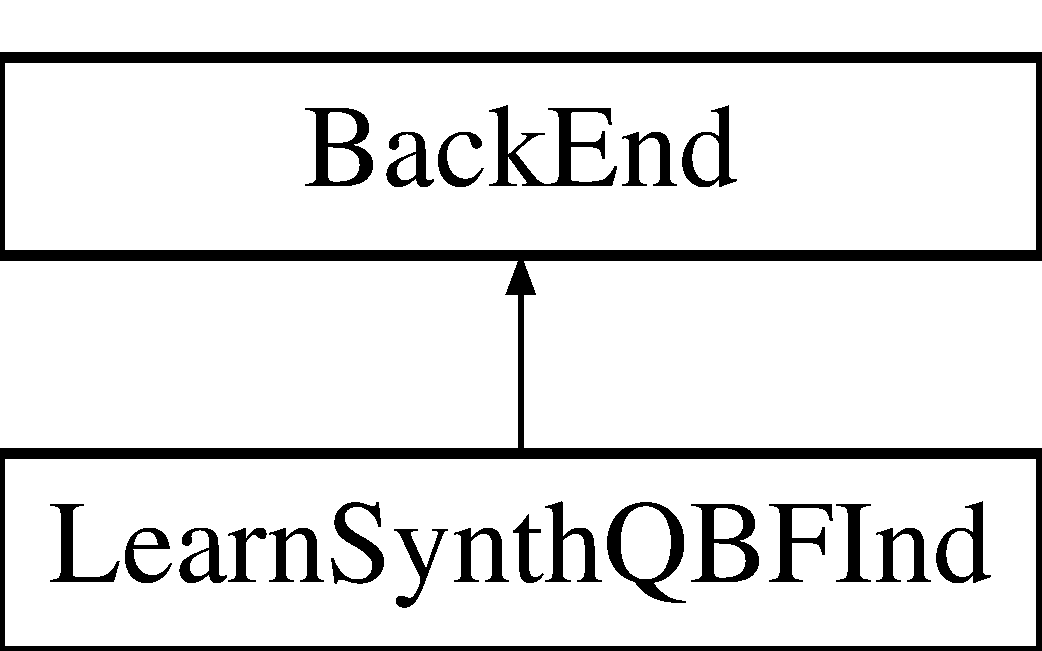
\includegraphics[height=2.000000cm]{classLearnSynthQBFInd}
\end{center}
\end{figure}
\subsection*{Public Member Functions}
\begin{DoxyCompactItemize}
\item 
\hyperlink{classLearnSynthQBFInd_a3e05b058bbff2f55eeb054e3968a3a70}{Learn\-Synth\-Q\-B\-F\-Ind} (\hyperlink{classCNFImplExtractor}{C\-N\-F\-Impl\-Extractor} $\ast$impl\-\_\-extractor)
\begin{DoxyCompactList}\small\item\em Constructor. \end{DoxyCompactList}\item 
virtual \hyperlink{classLearnSynthQBFInd_ae7c562c17f47985549499bb1ea6d4485}{$\sim$\-Learn\-Synth\-Q\-B\-F\-Ind} ()
\begin{DoxyCompactList}\small\item\em Destructor. \end{DoxyCompactList}\item 
virtual bool \hyperlink{classLearnSynthQBFInd_a6709343a109f82c427dcbc4a576d9c03}{run} ()
\begin{DoxyCompactList}\small\item\em Executes this back-\/end. \end{DoxyCompactList}\end{DoxyCompactItemize}
\subsection*{Protected Member Functions}
\begin{DoxyCompactItemize}
\item 
bool \hyperlink{classLearnSynthQBFInd_a41593ccf692af8948f4b1255fb13ffe5}{compute\-Winning\-Region} ()
\begin{DoxyCompactList}\small\item\em Computes the winning region and stores the result in \hyperlink{classLearnSynthQBFInd_ab8ce6031137413e90e0626bbdc734be0}{winning\-\_\-region\-\_\-}. \end{DoxyCompactList}\item 
bool \hyperlink{classLearnSynthQBFInd_a9a48eb17721b9c941689795e0913dc0b}{compute\-Winning\-Region\-One} ()
\begin{DoxyCompactList}\small\item\em Uses the standard method to compute the winning region, with inductive reasoning. \end{DoxyCompactList}\item 
bool \hyperlink{classLearnSynthQBFInd_a1665e16ff8fa78f696b1e3373db96edb}{compute\-Winning\-Region\-All} ()
\begin{DoxyCompactList}\small\item\em Computes the winning region, always computing all counterexample generalizations. \end{DoxyCompactList}\item 
bool \hyperlink{classLearnSynthQBFInd_a1a771069bb5352236c509593e8f18426}{compute\-Counterexample\-Q\-B\-F} (vector$<$ int $>$ \&ce)
\begin{DoxyCompactList}\small\item\em Computes a counterexample-\/state using a Q\-B\-F-\/solver with inductive reasoning. \end{DoxyCompactList}\item 
bool \hyperlink{classLearnSynthQBFInd_a0ddc68117f68cecdfd09231562f981c7}{compute\-Blocking\-Clause} (vector$<$ int $>$ \&ce, vector$<$ int $>$ \&blocking\-\_\-clause)
\begin{DoxyCompactList}\small\item\em Computes a blocking clause for a counterexample. \end{DoxyCompactList}\item 
bool \hyperlink{classLearnSynthQBFInd_a22e56037bf21941a2a2510eabd97b279}{compute\-All\-Blocking\-Clauses} (vector$<$ int $>$ \&ce, vector$<$ vector$<$ int $>$ $>$ \&blocking\-\_\-clauses)
\begin{DoxyCompactList}\small\item\em Computes all minimal blocking clauses for a counterexample. \end{DoxyCompactList}\item 
void \hyperlink{classLearnSynthQBFInd_a0f02719c7a3b6d928337f310dabff478}{reduce\-Existing\-Clauses} ()
\begin{DoxyCompactList}\small\item\em Tries to drop literals from clauses in the winning region. \end{DoxyCompactList}\item 
void \hyperlink{classLearnSynthQBFInd_a5c7c552e1e8db8dd80e53778d42e9627}{recompute\-Check\-C\-N\-F} (bool take\-\_\-small\-\_\-win=true)
\begin{DoxyCompactList}\small\item\em Recomputes the \hyperlink{classCNF}{C\-N\-F} (of the Q\-B\-F) that is used for computing counterexamples. \end{DoxyCompactList}\item 
void \hyperlink{classLearnSynthQBFInd_ae1ed892480cb3404d5ff1e7ee35b5a9c}{recompute\-Gen\-C\-N\-F} (bool take\-\_\-small\-\_\-win=true)
\begin{DoxyCompactList}\small\item\em Recomputes the \hyperlink{classCNF}{C\-N\-F} (of the Q\-B\-F) that is used for generalizing counterexamples. \end{DoxyCompactList}\item 
void \hyperlink{classLearnSynthQBFInd_a75417fbbe8b1bedbd1ef158299606929}{restrict\-To\-States} (vector$<$ int $>$ \&vec) const 
\begin{DoxyCompactList}\small\item\em Restricts a vector of literals (a cube or clause) to state-\/variables only. \end{DoxyCompactList}\item 
bool \hyperlink{classLearnSynthQBFInd_a5a34501e485a063d8120a2a79c39d9c9}{generalize\-Counterexample} (vector$<$ int $>$ \&ce, bool check\-\_\-sat=true) const 
\begin{DoxyCompactList}\small\item\em Generalizes a counterexample-\/state by dropping literals. \end{DoxyCompactList}\item 
int \hyperlink{classLearnSynthQBFInd_a106c202c2855e1d83e0074674fef51a9}{present\-To\-Previous} (int literal) const 
\begin{DoxyCompactList}\small\item\em Returns the previous-\/state copy of a literal. \end{DoxyCompactList}\item 
void \hyperlink{classLearnSynthQBFInd_a9a336d870d76716b356a2870eb1bf9b7}{present\-To\-Previous} (vector$<$ int $>$ \&cube\-\_\-or\-\_\-clause) const 
\begin{DoxyCompactList}\small\item\em Computes the previous-\/state copy of a cube or clause. \end{DoxyCompactList}\item 
void \hyperlink{classLearnSynthQBFInd_a50be93ab3f6b7bd38c1f607dcb4b91b8}{present\-To\-Previous} (\hyperlink{classCNF}{C\-N\-F} \&cnf) const 
\begin{DoxyCompactList}\small\item\em Computes the previous-\/state copy of a \hyperlink{classCNF}{C\-N\-F}. \end{DoxyCompactList}\item 
void \hyperlink{classLearnSynthQBFInd_abb1bed24925bb028eeb33b2bfb8914a1}{debug\-Check\-Win\-Reg\-Reach} () const 
\begin{DoxyCompactList}\small\item\em Checks a winning region computed with optimization R\-C for correctness. \end{DoxyCompactList}\end{DoxyCompactItemize}
\subsection*{Protected Attributes}
\begin{DoxyCompactItemize}
\item 
\hyperlink{classCNF}{C\-N\-F} \hyperlink{classLearnSynthQBFInd_ab8ce6031137413e90e0626bbdc734be0}{winning\-\_\-region\-\_\-}
\begin{DoxyCompactList}\small\item\em The current over-\/approximation of the winning region. \end{DoxyCompactList}\item 
\hyperlink{classCNF}{C\-N\-F} \hyperlink{classLearnSynthQBFInd_a333c9336ba28a2c41f252a3051a59581}{winning\-\_\-region\-\_\-large\-\_\-}
\begin{DoxyCompactList}\small\item\em The current over-\/approximation of the winning region in an uncompressed form. \end{DoxyCompactList}\item 
\hyperlink{classLearnStatisticsQBF}{Learn\-Statistics\-Q\-B\-F} \hyperlink{classLearnSynthQBFInd_af83f4253aeedaed56cb789369b054724}{statistics\-\_\-}
\begin{DoxyCompactList}\small\item\em Stores and maintains statistics and performance measures. \end{DoxyCompactList}\item 
\hyperlink{classQBFSolver}{Q\-B\-F\-Solver} $\ast$ \hyperlink{classLearnSynthQBFInd_ada2a2526b313b2ba4bb9d717fb63362d}{qbf\-\_\-solver\-\_\-}
\begin{DoxyCompactList}\small\item\em The Q\-B\-F-\/solver used for all queries. \end{DoxyCompactList}\item 
vector$<$ pair$<$ \hyperlink{classVarInfo_a64d1da76cf84fe674e5fef9764ef11cf}{Var\-Info\-::\-Var\-Kind}, \\*
\hyperlink{classQBFSolver_ac091e263cb55286cc07b2451bcf4d3c7}{Q\-B\-F\-Solver\-::\-Quant} $>$ $>$ \hyperlink{classLearnSynthQBFInd_ab9287e0b57dbf85dab6e7f7caf30cd13}{check\-\_\-quant\-\_\-}
\begin{DoxyCompactList}\small\item\em The quantifier prefix of the Q\-B\-F for computing counterexamples. \end{DoxyCompactList}\item 
\hyperlink{classCNF}{C\-N\-F} \hyperlink{classLearnSynthQBFInd_ac90a4574da82c96888db219291368554}{check\-\_\-cnf\-\_\-}
\begin{DoxyCompactList}\small\item\em The \hyperlink{classCNF}{C\-N\-F} matrix of the Q\-B\-F for computing counterexamples. \end{DoxyCompactList}\item 
vector$<$ pair$<$ \hyperlink{classVarInfo_a64d1da76cf84fe674e5fef9764ef11cf}{Var\-Info\-::\-Var\-Kind}, \\*
\hyperlink{classQBFSolver_ac091e263cb55286cc07b2451bcf4d3c7}{Q\-B\-F\-Solver\-::\-Quant} $>$ $>$ \hyperlink{classLearnSynthQBFInd_a1a20b68cc735e4bbc0cc7030329acb4d}{gen\-\_\-quant\-\_\-}
\begin{DoxyCompactList}\small\item\em The quantifier prefix of the Q\-B\-F for generalizing counterexamples. \end{DoxyCompactList}\item 
\hyperlink{classCNF}{C\-N\-F} \hyperlink{classLearnSynthQBFInd_ad61b112cfcc60506f7b21c9ea9267b37}{generalize\-\_\-clause\-\_\-cnf\-\_\-}
\begin{DoxyCompactList}\small\item\em The \hyperlink{classCNF}{C\-N\-F} matrix of the Q\-B\-F for generalizing counterexamples. \end{DoxyCompactList}\item 
vector$<$ int $>$ \hyperlink{classLearnSynthQBFInd_a8047ab13c44736c39c11f9c0b48e29cf}{current\-\_\-to\-\_\-previous\-\_\-map\-\_\-}
\begin{DoxyCompactList}\small\item\em A map from present-\/state variables to their previous-\/state copy. \end{DoxyCompactList}\item 
int \hyperlink{classLearnSynthQBFInd_a36e64e8ac156ca4978e73be5493de782}{current\-\_\-state\-\_\-is\-\_\-initial\-\_\-}
\begin{DoxyCompactList}\small\item\em A literal that is true if the current state is initial and false otherwise. \end{DoxyCompactList}\item 
\hyperlink{classCNF}{C\-N\-F} \hyperlink{classLearnSynthQBFInd_ad99eafb7ee9134115f9fbe986e5eb0c5}{prev\-\_\-trans\-\_\-or\-\_\-initial\-\_\-}
\begin{DoxyCompactList}\small\item\em Says\-: the current state is initial or the previous transition relation holds. \end{DoxyCompactList}\item 
\hyperlink{classCNF}{C\-N\-F} \hyperlink{classLearnSynthQBFInd_a6854254065f912e3d5fe07a1b895f1c6}{check\-\_\-reach\-\_\-}
\begin{DoxyCompactList}\small\item\em Says\-: \hyperlink{classLearnSynthQBFInd_ad99eafb7ee9134115f9fbe986e5eb0c5}{prev\-\_\-trans\-\_\-or\-\_\-initial\-\_\-} and the current state is different from the previous. \end{DoxyCompactList}\item 
bool \hyperlink{classLearnSynthQBFInd_af87e4a2c1d17c4c5bc398082d6d3e365}{do\-\_\-reach\-\_\-check\-\_\-}
\begin{DoxyCompactList}\small\item\em Enables or disables optimization R\-C. \end{DoxyCompactList}\item 
\hyperlink{classCNFImplExtractor}{C\-N\-F\-Impl\-Extractor} $\ast$ \hyperlink{classLearnSynthQBFInd_a8c285416b6f27e86bdda92fd578327b8}{impl\-\_\-extractor\-\_\-}
\begin{DoxyCompactList}\small\item\em The engine to use for circuit extraction. \end{DoxyCompactList}\end{DoxyCompactItemize}
\subsection*{Private Member Functions}
\begin{DoxyCompactItemize}
\item 
\hyperlink{classLearnSynthQBFInd_a55edd29ba2b93167b7d7b2bf6b835673}{Learn\-Synth\-Q\-B\-F\-Ind} (const \hyperlink{classLearnSynthQBFInd}{Learn\-Synth\-Q\-B\-F\-Ind} \&other)
\begin{DoxyCompactList}\small\item\em Copy constructor. \end{DoxyCompactList}\item 
\hyperlink{classLearnSynthQBFInd}{Learn\-Synth\-Q\-B\-F\-Ind} \& \hyperlink{classLearnSynthQBFInd_a411e8fa65ea22877c0fa9180f31120f9}{operator=} (const \hyperlink{classLearnSynthQBFInd}{Learn\-Synth\-Q\-B\-F\-Ind} \&other)
\begin{DoxyCompactList}\small\item\em Assignment operator. \end{DoxyCompactList}\end{DoxyCompactItemize}


\subsection{Detailed Description}
Implements a learning-\/based synthesis with inductive reachability reasoning. 

This class is almost an exact copy of \hyperlink{classLearnSynthQBF}{Learn\-Synth\-Q\-B\-F}. Hence, we refer to the documentation of \hyperlink{classLearnSynthQBF}{Learn\-Synth\-Q\-B\-F} for an explanation of the basic working principle. The main difference is that this class uses a reachability optimization that is inspired by the concept of inductiveness relative to a certain clause set used in I\-C3. Refer to the V\-M\-C\-A\-I'14 publication \char`\"{}\-S\-A\-T-\/\-Based Synthesis Methods for Safety Specs\char`\"{} for a detailed explanation how (and why) this works. The class \hyperlink{classLearnSynthQBF}{Learn\-Synth\-Q\-B\-F} computes counterexamples by solving\-: exists x,i\-: forall c\-: exists x',tmp\-: F(x) \& T(x,i,c,x') \& !\-F(x') \par
 and generalizes them by checking exists x\-: forall i\-: exists c,x',tmp\-: s \& F(x) \& T(x,i,c,x') \& F(x') \par
 repeatedly, where s is the counterexample and F is the current over-\/approximation of the winning region.

We know that F(x) is never left by the final implementation. Hence, F is an over-\/approximation of the reachable states. Now if a state s is not initial and !s \& F \& T =$>$ !s', then we know by induction that the state s is unreachable. We can disregard unreachable states both in the computation of counterexamples as well as during the generalization. This is done by gluing the constraints !s \& F \& T =$>$ !s' and !\-I(s) to the generalization and check queries as following. The check query becomes\-: \par
 ~ exists x$\ast$,i$\ast$,c$\ast$,x,i\-: forall c\-: exists x',tmp\-: (I(x) $|$ (x$\ast$ != x) \& F(x$\ast$) \& T(x$\ast$, i$\ast$, c$\ast$, x)) \& F(x) \& T(x,i,c,x') \& !\-F(x') \par
 where x$\ast$, i$\ast$ and c$\ast$ are the previous-\/state copy of x,i,c. The query now says\-: find a counterexample-\/state x that is either initial or has a predecessor x$\ast$ in F such that x$\ast$ is different from x. (Otherwise the counterexample-\/state is unreachable.) The generalization query becomes\-: \par
 ~ exists x$\ast$,i$\ast$,c$\ast$,x\-: forall i\-: exists c,x',tmp\-: (I(x) $|$ F(x$\ast$) \& !s$\ast$ \& T(x$\ast$, i$\ast$, c$\ast$, x)) \& s \& F(x) \& T(x,i,c,x') \& F(x') \par
 where x$\ast$, i$\ast$ and c$\ast$ are the previous-\/state copy of x,i,c. The query now says\-: a state that prevents generalization must be either initial or have a predecessor in F \& !s. Otherwise it is unreachable and we do not care. This means that we can remove states that are winning for the protagonist from the winning region of they are unreachalbe in the final implementation.

The modification of the generalization is called optimization R\-G in the V\-M\-C\-A\-I paper. The modification of the counterexample-\/computation is called optimization R\-C. Depending on the command-\/line parameters (--mode) this class performs either just one or both optimizations. Experiments suggest that optimization R\-G is often beneficial, while optimization R\-C is usually not. Optimization R\-C leads to a winning region which cannot be turned into a circuit with the standard method.

\begin{DoxyRefDesc}{Todo}
\item[\hyperlink{todo__todo000003}{Todo}]Turning a winning region that was computed with optimization R\-C into a circuit is not yet implemented. However, since optimization R\-C does not increase the performance in our experiments (in contrast to optimization R\-G), this is not a severe issue at the moment. We can consider optimization R\-C as experiment that did not work out well. \end{DoxyRefDesc}
\begin{DoxyNote}{Note}
This class is experimental. 
\end{DoxyNote}
\begin{DoxyAuthor}{Author}
Robert Koenighofer (\href{mailto:robert.koenighofer@iaik.tugraz.at}{\tt robert.\-koenighofer@iaik.\-tugraz.\-at}) 
\end{DoxyAuthor}
\begin{DoxyVersion}{Version}
1.\-1.\-0 
\end{DoxyVersion}


Definition at line 100 of file Learn\-Synth\-Q\-B\-F\-Ind.\-h.



\subsection{Constructor \& Destructor Documentation}
\hypertarget{classLearnSynthQBFInd_a3e05b058bbff2f55eeb054e3968a3a70}{\index{Learn\-Synth\-Q\-B\-F\-Ind@{Learn\-Synth\-Q\-B\-F\-Ind}!Learn\-Synth\-Q\-B\-F\-Ind@{Learn\-Synth\-Q\-B\-F\-Ind}}
\index{Learn\-Synth\-Q\-B\-F\-Ind@{Learn\-Synth\-Q\-B\-F\-Ind}!LearnSynthQBFInd@{Learn\-Synth\-Q\-B\-F\-Ind}}
\subsubsection[{Learn\-Synth\-Q\-B\-F\-Ind}]{\setlength{\rightskip}{0pt plus 5cm}Learn\-Synth\-Q\-B\-F\-Ind\-::\-Learn\-Synth\-Q\-B\-F\-Ind (
\begin{DoxyParamCaption}
\item[{{\bf C\-N\-F\-Impl\-Extractor} $\ast$}]{impl\-\_\-extractor}
\end{DoxyParamCaption}
)}}\label{classLearnSynthQBFInd_a3e05b058bbff2f55eeb054e3968a3a70}


Constructor. 


\begin{DoxyParams}{Parameters}
{\em impl\-\_\-extractor} & The engine to use for circuit extraction. It will be deleted by this class. \\
\hline
\end{DoxyParams}


Definition at line 40 of file Learn\-Synth\-Q\-B\-F\-Ind.\-cpp.



References Q\-B\-F\-Solver\-::\-A, C\-N\-F\-::add2\-Lit\-Clause(), C\-N\-F\-::add3\-Lit\-Clause(), C\-N\-F\-::add\-Clause(), C\-N\-F\-::add\-C\-N\-F(), check\-\_\-quant\-\_\-, check\-\_\-reach\-\_\-, Var\-Manager\-::create\-Fresh\-Prev\-Var(), Var\-Manager\-::create\-Fresh\-Tmp\-Var(), Var\-Info\-::\-C\-T\-R\-L, current\-\_\-state\-\_\-is\-\_\-initial\-\_\-, current\-\_\-to\-\_\-previous\-\_\-map\-\_\-, do\-\_\-reach\-\_\-check\-\_\-, Q\-B\-F\-Solver\-::\-E, gen\-\_\-quant\-\_\-, C\-N\-F\-::get\-Clauses(), Var\-Manager\-::get\-Max\-C\-N\-F\-Var(), A\-I\-G2\-C\-N\-F\-::get\-Trans(), Var\-Manager\-::get\-Vars\-Of\-Type(), Var\-Info\-::\-I\-N\-P\-U\-T, Var\-Manager\-::instance(), Options\-::instance(), A\-I\-G2\-C\-N\-F\-::instance(), Var\-Info\-::\-N\-E\-X\-T\-\_\-\-S\-T\-A\-T\-E, Var\-Info\-::\-P\-R\-E\-S\-\_\-\-S\-T\-A\-T\-E, present\-To\-Previous(), Var\-Info\-::\-P\-R\-E\-V, prev\-\_\-trans\-\_\-or\-\_\-initial\-\_\-, C\-N\-F\-::swap\-With(), and Var\-Info\-::\-T\-M\-P.

\hypertarget{classLearnSynthQBFInd_ae7c562c17f47985549499bb1ea6d4485}{\index{Learn\-Synth\-Q\-B\-F\-Ind@{Learn\-Synth\-Q\-B\-F\-Ind}!$\sim$\-Learn\-Synth\-Q\-B\-F\-Ind@{$\sim$\-Learn\-Synth\-Q\-B\-F\-Ind}}
\index{$\sim$\-Learn\-Synth\-Q\-B\-F\-Ind@{$\sim$\-Learn\-Synth\-Q\-B\-F\-Ind}!LearnSynthQBFInd@{Learn\-Synth\-Q\-B\-F\-Ind}}
\subsubsection[{$\sim$\-Learn\-Synth\-Q\-B\-F\-Ind}]{\setlength{\rightskip}{0pt plus 5cm}Learn\-Synth\-Q\-B\-F\-Ind\-::$\sim$\-Learn\-Synth\-Q\-B\-F\-Ind (
\begin{DoxyParamCaption}
{}
\end{DoxyParamCaption}
)\hspace{0.3cm}{\ttfamily [virtual]}}}\label{classLearnSynthQBFInd_ae7c562c17f47985549499bb1ea6d4485}


Destructor. 



Definition at line 137 of file Learn\-Synth\-Q\-B\-F\-Ind.\-cpp.



References impl\-\_\-extractor\-\_\-, and qbf\-\_\-solver\-\_\-.

\hypertarget{classLearnSynthQBFInd_a55edd29ba2b93167b7d7b2bf6b835673}{\index{Learn\-Synth\-Q\-B\-F\-Ind@{Learn\-Synth\-Q\-B\-F\-Ind}!Learn\-Synth\-Q\-B\-F\-Ind@{Learn\-Synth\-Q\-B\-F\-Ind}}
\index{Learn\-Synth\-Q\-B\-F\-Ind@{Learn\-Synth\-Q\-B\-F\-Ind}!LearnSynthQBFInd@{Learn\-Synth\-Q\-B\-F\-Ind}}
\subsubsection[{Learn\-Synth\-Q\-B\-F\-Ind}]{\setlength{\rightskip}{0pt plus 5cm}Learn\-Synth\-Q\-B\-F\-Ind\-::\-Learn\-Synth\-Q\-B\-F\-Ind (
\begin{DoxyParamCaption}
\item[{const {\bf Learn\-Synth\-Q\-B\-F\-Ind} \&}]{other}
\end{DoxyParamCaption}
)\hspace{0.3cm}{\ttfamily [private]}}}\label{classLearnSynthQBFInd_a55edd29ba2b93167b7d7b2bf6b835673}


Copy constructor. 

The copy constructor is disabled (set private) and not implemented.


\begin{DoxyParams}{Parameters}
{\em other} & The source for creating the copy. \\
\hline
\end{DoxyParams}


\subsection{Member Function Documentation}
\hypertarget{classLearnSynthQBFInd_a22e56037bf21941a2a2510eabd97b279}{\index{Learn\-Synth\-Q\-B\-F\-Ind@{Learn\-Synth\-Q\-B\-F\-Ind}!compute\-All\-Blocking\-Clauses@{compute\-All\-Blocking\-Clauses}}
\index{compute\-All\-Blocking\-Clauses@{compute\-All\-Blocking\-Clauses}!LearnSynthQBFInd@{Learn\-Synth\-Q\-B\-F\-Ind}}
\subsubsection[{compute\-All\-Blocking\-Clauses}]{\setlength{\rightskip}{0pt plus 5cm}bool Learn\-Synth\-Q\-B\-F\-Ind\-::compute\-All\-Blocking\-Clauses (
\begin{DoxyParamCaption}
\item[{vector$<$ int $>$ \&}]{ce, }
\item[{vector$<$ vector$<$ int $>$ $>$ \&}]{blocking\-\_\-clauses}
\end{DoxyParamCaption}
)\hspace{0.3cm}{\ttfamily [protected]}}}\label{classLearnSynthQBFInd_a22e56037bf21941a2a2510eabd97b279}


Computes all minimal blocking clauses for a counterexample. 

This method works like \hyperlink{classLearnSynthQBF_affa7b4583cc17d01f4c82fd57e763e1f}{Learn\-Synth\-Q\-B\-F\-::compute\-All\-Blocking\-Clauses()} but using inductive reasoning regarding reachable states as an optimization. That is, instead of solving \par
 ~ exists x\-: forall i\-: exists c,x',tmp\-: s \& F(x) \& T(x,i,c,x') \& F(x') \par
 where s is the counterexample-\/state to generalize, we solve \par
 ~ exists x$\ast$,i$\ast$,c$\ast$,x\-: forall i\-: exists c,x',tmp\-: (I(x) $|$ F(x$\ast$) \& !s$\ast$ \& T(x$\ast$, i$\ast$, c$\ast$, x)) \& s \& F(x) \& T(x,i,c,x') \& F(x') \par
 The query now says\-: a state that prevents generalization must be either initial or have a predecessor in F \& !s. Otherwise it is unreachable and we do not care. This means that we can remove states that are winning for the protagonist from the winning region of they are unreachable in the final implementation.


\begin{DoxyParams}{Parameters}
{\em ce} & The counterexample to block. It is a full or partial cube over the state variables. \\
\hline
{\em blocking\-\_\-clauses} & An empty vector. It is used to store the computed blocking clauses. The counterexample falsifies all blocking clauses in this vector. \\
\hline
\end{DoxyParams}
\begin{DoxyReturn}{Returns}
False if one of the blocking clauses blocks the initial state. This means that the initial state is removed from the winning region, i.\-e., the specification is unrealizable. True is returned otherwise. 
\end{DoxyReturn}


Definition at line 364 of file Learn\-Synth\-Q\-B\-F\-Ind.\-cpp.



References C\-N\-F\-::add\-Clause(), Utils\-::contains\-Init(), generalize\-\_\-clause\-\_\-cnf\-\_\-, generalize\-Counterexample(), Utils\-::intersection\-Empty(), Utils\-::negate\-Literals(), Learn\-Statistics\-Q\-B\-F\-::notify\-After\-Cube\-Min(), Learn\-Statistics\-Q\-B\-F\-::notify\-Before\-Cube\-Min(), Learn\-Statistics\-Q\-B\-F\-::notify\-Cube\-Min(), present\-To\-Previous(), Utils\-::remove(), statistics\-\_\-, and Utils\-::swap\-Present\-To\-Next().



Referenced by compute\-Winning\-Region\-All().

\hypertarget{classLearnSynthQBFInd_a0ddc68117f68cecdfd09231562f981c7}{\index{Learn\-Synth\-Q\-B\-F\-Ind@{Learn\-Synth\-Q\-B\-F\-Ind}!compute\-Blocking\-Clause@{compute\-Blocking\-Clause}}
\index{compute\-Blocking\-Clause@{compute\-Blocking\-Clause}!LearnSynthQBFInd@{Learn\-Synth\-Q\-B\-F\-Ind}}
\subsubsection[{compute\-Blocking\-Clause}]{\setlength{\rightskip}{0pt plus 5cm}bool Learn\-Synth\-Q\-B\-F\-Ind\-::compute\-Blocking\-Clause (
\begin{DoxyParamCaption}
\item[{vector$<$ int $>$ \&}]{ce, }
\item[{vector$<$ int $>$ \&}]{blocking\-\_\-clause}
\end{DoxyParamCaption}
)\hspace{0.3cm}{\ttfamily [protected]}}}\label{classLearnSynthQBFInd_a0ddc68117f68cecdfd09231562f981c7}


Computes a blocking clause for a counterexample. 

This method works like \hyperlink{classLearnSynthQBF_a73856a79be3fb7e260485bcda7c31f80}{Learn\-Synth\-Q\-B\-F\-::compute\-Blocking\-Clause()} but using inductive reasoning regarding reachable states as an optimization. That is, instead of solving \par
 ~ exists x\-: forall i\-: exists c,x',tmp\-: s \& F(x) \& T(x,i,c,x') \& F(x') \par
 where s is the counterexample-\/state to generalize, we solve \par
 ~ exists x$\ast$,i$\ast$,c$\ast$,x\-: forall i\-: exists c,x',tmp\-: (I(x) $|$ F(x$\ast$) \& !s$\ast$ \& T(x$\ast$, i$\ast$, c$\ast$, x)) \& s \& F(x) \& T(x,i,c,x') \& F(x') \par
 The query now says\-: a state that prevents generalization must be either initial or have a predecessor in F \& !s. Otherwise it is unreachable and we do not care. This means that we can remove states that are winning for the protagonist from the winning region of they are unreachable in the final implementation.


\begin{DoxyParams}{Parameters}
{\em ce} & The counterexample to block. It is a full or partial cube over the state variables. \\
\hline
{\em blocking\-\_\-clause} & An empty vector. It is used to store the computed blocking clause. The counterexample falsifies the blocking clause. \\
\hline
\end{DoxyParams}
\begin{DoxyReturn}{Returns}
False if the blocking clause blocks the initial state. This means that the initial state is removed from the winning region, i.\-e., the specification is unrealizable. True is returned otherwise. 
\end{DoxyReturn}


Definition at line 346 of file Learn\-Synth\-Q\-B\-F\-Ind.\-cpp.



References Utils\-::contains\-Init(), generalize\-Counterexample(), L\-\_\-\-D\-B\-G, Utils\-::negate\-Literals(), Learn\-Statistics\-Q\-B\-F\-::notify\-After\-Cube\-Min(), Learn\-Statistics\-Q\-B\-F\-::notify\-Before\-Cube\-Min(), Utils\-::randomize(), and statistics\-\_\-.



Referenced by compute\-Winning\-Region\-One().

\hypertarget{classLearnSynthQBFInd_a1a771069bb5352236c509593e8f18426}{\index{Learn\-Synth\-Q\-B\-F\-Ind@{Learn\-Synth\-Q\-B\-F\-Ind}!compute\-Counterexample\-Q\-B\-F@{compute\-Counterexample\-Q\-B\-F}}
\index{compute\-Counterexample\-Q\-B\-F@{compute\-Counterexample\-Q\-B\-F}!LearnSynthQBFInd@{Learn\-Synth\-Q\-B\-F\-Ind}}
\subsubsection[{compute\-Counterexample\-Q\-B\-F}]{\setlength{\rightskip}{0pt plus 5cm}bool Learn\-Synth\-Q\-B\-F\-Ind\-::compute\-Counterexample\-Q\-B\-F (
\begin{DoxyParamCaption}
\item[{vector$<$ int $>$ \&}]{ce}
\end{DoxyParamCaption}
)\hspace{0.3cm}{\ttfamily [protected]}}}\label{classLearnSynthQBFInd_a1a771069bb5352236c509593e8f18426}


Computes a counterexample-\/state using a Q\-B\-F-\/solver with inductive reasoning. 

This method works like \hyperlink{classLearnSynthQBF_a04b8dd6e26d646a6f197afb362168408}{Learn\-Synth\-Q\-B\-F\-::compute\-Counterexample\-Q\-B\-F()} but using inductive reasoning regarding reachable states as an optimization. That is, instead of solving \par
 ~ exists x,i\-: forall c\-: exists x',tmp\-: F(x) \& T(x,i,c,x') \& !\-F(x') \par
 we solve \par
 ~ exists x$\ast$,i$\ast$,c$\ast$,x,i\-: forall c\-: exists x',tmp\-: (I(x) $|$ (x$\ast$ != x) \& F(x$\ast$) \& T(x$\ast$, i$\ast$, c$\ast$, x)) \& F(x) \& T(x,i,c,x') \& !\-F(x') \par
 to obtain a counterexample. The query now says\-: find a counterexample-\/state x that is either initial or has a predecessor x$\ast$ in F such that x$\ast$ is different from x. (Otherwise the counterexample-\/state is unreachable.)

If optimization R\-C is disabled (\hyperlink{classLearnSynthQBFInd_af87e4a2c1d17c4c5bc398082d6d3e365}{do\-\_\-reach\-\_\-check\-\_\-} is false), then counterexamples are computed in the standard way.


\begin{DoxyParams}{Parameters}
{\em ce} & An empty vector. The computed counterexample is stored in this vector in form of a cube over the state variables. The cube does not necessarily contain all state variables. If some state variables are irrelevant, then they may be omitted. \\
\hline
\end{DoxyParams}
\begin{DoxyReturn}{Returns}
True if a counterexample was found, false if no counterexample exists. 
\end{DoxyReturn}


Definition at line 335 of file Learn\-Synth\-Q\-B\-F\-Ind.\-cpp.



References check\-\_\-cnf\-\_\-, check\-\_\-quant\-\_\-, Q\-B\-F\-Solver\-::is\-Sat\-Model(), Learn\-Statistics\-Q\-B\-F\-::notify\-After\-Compute\-Cube(), Learn\-Statistics\-Q\-B\-F\-::notify\-Before\-Compute\-Cube(), qbf\-\_\-solver\-\_\-, restrict\-To\-States(), and statistics\-\_\-.



Referenced by compute\-Winning\-Region\-All(), and compute\-Winning\-Region\-One().

\hypertarget{classLearnSynthQBFInd_a41593ccf692af8948f4b1255fb13ffe5}{\index{Learn\-Synth\-Q\-B\-F\-Ind@{Learn\-Synth\-Q\-B\-F\-Ind}!compute\-Winning\-Region@{compute\-Winning\-Region}}
\index{compute\-Winning\-Region@{compute\-Winning\-Region}!LearnSynthQBFInd@{Learn\-Synth\-Q\-B\-F\-Ind}}
\subsubsection[{compute\-Winning\-Region}]{\setlength{\rightskip}{0pt plus 5cm}bool Learn\-Synth\-Q\-B\-F\-Ind\-::compute\-Winning\-Region (
\begin{DoxyParamCaption}
{}
\end{DoxyParamCaption}
)\hspace{0.3cm}{\ttfamily [protected]}}}\label{classLearnSynthQBFInd_a41593ccf692af8948f4b1255fb13ffe5}


Computes the winning region and stores the result in \hyperlink{classLearnSynthQBFInd_ab8ce6031137413e90e0626bbdc734be0}{winning\-\_\-region\-\_\-}. 

Depending on the command-\/line parameters (--mode) this method calls one of 
\begin{DoxyItemize}
\item \hyperlink{classLearnSynthQBFInd_a9a48eb17721b9c941689795e0913dc0b}{compute\-Winning\-Region\-One()} 
\item \hyperlink{classLearnSynthQBFInd_a1665e16ff8fa78f696b1e3373db96edb}{compute\-Winning\-Region\-All()} 
\end{DoxyItemize}

\begin{DoxyReturn}{Returns}
True if the specification was realizable, false otherwise. 
\end{DoxyReturn}


Definition at line 178 of file Learn\-Synth\-Q\-B\-F\-Ind.\-cpp.



References compute\-Winning\-Region\-All(), compute\-Winning\-Region\-One(), Utils\-::debug\-Check\-Win\-Reg(), debug\-Check\-Win\-Reg\-Reach(), do\-\_\-reach\-\_\-check\-\_\-, Options\-::get\-Back\-End\-Mode(), Options\-::instance(), and winning\-\_\-region\-\_\-.



Referenced by run().

\hypertarget{classLearnSynthQBFInd_a1665e16ff8fa78f696b1e3373db96edb}{\index{Learn\-Synth\-Q\-B\-F\-Ind@{Learn\-Synth\-Q\-B\-F\-Ind}!compute\-Winning\-Region\-All@{compute\-Winning\-Region\-All}}
\index{compute\-Winning\-Region\-All@{compute\-Winning\-Region\-All}!LearnSynthQBFInd@{Learn\-Synth\-Q\-B\-F\-Ind}}
\subsubsection[{compute\-Winning\-Region\-All}]{\setlength{\rightskip}{0pt plus 5cm}bool Learn\-Synth\-Q\-B\-F\-Ind\-::compute\-Winning\-Region\-All (
\begin{DoxyParamCaption}
{}
\end{DoxyParamCaption}
)\hspace{0.3cm}{\ttfamily [protected]}}}\label{classLearnSynthQBFInd_a1665e16ff8fa78f696b1e3373db96edb}


Computes the winning region, always computing all counterexample generalizations. 

This method works like \hyperlink{classLearnSynthQBF_ac538cd53082bad1c8c45a7e178dfa4cb}{Learn\-Synth\-Q\-B\-F\-::compute\-Winning\-Region\-One()} but using inductive reasoning regarding reachable states as an optimization (as explained in the description of the class).

\begin{DoxyReturn}{Returns}
True if the specification was realizable, false otherwise. 
\end{DoxyReturn}


Definition at line 269 of file Learn\-Synth\-Q\-B\-F\-Ind.\-cpp.



References C\-N\-F\-::add\-Clause\-And\-Simplify(), check\-\_\-cnf\-\_\-, C\-N\-F\-::clear(), Utils\-::compress\-State\-C\-N\-F(), compute\-All\-Blocking\-Clauses(), compute\-Counterexample\-Q\-B\-F(), Var\-Info\-::\-C\-T\-R\-L, Logger\-::\-D\-B\-G, Utils\-::debug\-Print(), generalize\-\_\-clause\-\_\-cnf\-\_\-, C\-N\-F\-::get\-Nr\-Of\-Clauses(), C\-N\-F\-::get\-Nr\-Of\-Lits(), A\-I\-G2\-C\-N\-F\-::get\-Safe\-States(), Var\-Manager\-::get\-Vars\-Of\-Type(), Var\-Info\-::\-I\-N\-P\-U\-T, Var\-Manager\-::instance(), Logger\-::instance(), A\-I\-G2\-C\-N\-F\-::instance(), Logger\-::is\-Enabled(), L\-\_\-\-D\-B\-G, Learn\-Statistics\-Q\-B\-F\-::log\-Statistics(), Var\-Info\-::\-P\-R\-E\-S\-\_\-\-S\-T\-A\-T\-E, recompute\-Check\-C\-N\-F(), recompute\-Gen\-C\-N\-F(), reduce\-Existing\-Clauses(), statistics\-\_\-, winning\-\_\-region\-\_\-, and winning\-\_\-region\-\_\-large\-\_\-.



Referenced by compute\-Winning\-Region().

\hypertarget{classLearnSynthQBFInd_a9a48eb17721b9c941689795e0913dc0b}{\index{Learn\-Synth\-Q\-B\-F\-Ind@{Learn\-Synth\-Q\-B\-F\-Ind}!compute\-Winning\-Region\-One@{compute\-Winning\-Region\-One}}
\index{compute\-Winning\-Region\-One@{compute\-Winning\-Region\-One}!LearnSynthQBFInd@{Learn\-Synth\-Q\-B\-F\-Ind}}
\subsubsection[{compute\-Winning\-Region\-One}]{\setlength{\rightskip}{0pt plus 5cm}bool Learn\-Synth\-Q\-B\-F\-Ind\-::compute\-Winning\-Region\-One (
\begin{DoxyParamCaption}
{}
\end{DoxyParamCaption}
)\hspace{0.3cm}{\ttfamily [protected]}}}\label{classLearnSynthQBFInd_a9a48eb17721b9c941689795e0913dc0b}


Uses the standard method to compute the winning region, with inductive reasoning. 

This method works like \hyperlink{classLearnSynthQBF_ac538cd53082bad1c8c45a7e178dfa4cb}{Learn\-Synth\-Q\-B\-F\-::compute\-Winning\-Region\-One()} but using inductive reasoning regarding reachable states as an optimization (as explained in the description of the class).

\begin{DoxyReturn}{Returns}
True if the specification was realizable, false otherwise. 
\end{DoxyReturn}


Definition at line 197 of file Learn\-Synth\-Q\-B\-F\-Ind.\-cpp.



References C\-N\-F\-::add\-Clause\-And\-Simplify(), check\-\_\-cnf\-\_\-, C\-N\-F\-::clear(), Utils\-::compress\-State\-C\-N\-F(), compute\-Blocking\-Clause(), compute\-Counterexample\-Q\-B\-F(), Var\-Info\-::\-C\-T\-R\-L, Logger\-::\-D\-B\-G, Utils\-::debug\-Print(), generalize\-\_\-clause\-\_\-cnf\-\_\-, C\-N\-F\-::get\-Nr\-Of\-Clauses(), C\-N\-F\-::get\-Nr\-Of\-Lits(), A\-I\-G2\-C\-N\-F\-::get\-Safe\-States(), Var\-Manager\-::get\-Vars\-Of\-Type(), Var\-Info\-::\-I\-N\-P\-U\-T, Var\-Manager\-::instance(), Logger\-::instance(), A\-I\-G2\-C\-N\-F\-::instance(), Logger\-::is\-Enabled(), L\-\_\-\-D\-B\-G, Learn\-Statistics\-Q\-B\-F\-::log\-Statistics(), Var\-Info\-::\-P\-R\-E\-S\-\_\-\-S\-T\-A\-T\-E, present\-To\-Previous(), recompute\-Check\-C\-N\-F(), recompute\-Gen\-C\-N\-F(), statistics\-\_\-, Utils\-::swap\-Present\-To\-Next(), winning\-\_\-region\-\_\-, and winning\-\_\-region\-\_\-large\-\_\-.



Referenced by compute\-Winning\-Region().

\hypertarget{classLearnSynthQBFInd_abb1bed24925bb028eeb33b2bfb8914a1}{\index{Learn\-Synth\-Q\-B\-F\-Ind@{Learn\-Synth\-Q\-B\-F\-Ind}!debug\-Check\-Win\-Reg\-Reach@{debug\-Check\-Win\-Reg\-Reach}}
\index{debug\-Check\-Win\-Reg\-Reach@{debug\-Check\-Win\-Reg\-Reach}!LearnSynthQBFInd@{Learn\-Synth\-Q\-B\-F\-Ind}}
\subsubsection[{debug\-Check\-Win\-Reg\-Reach}]{\setlength{\rightskip}{0pt plus 5cm}void Learn\-Synth\-Q\-B\-F\-Ind\-::debug\-Check\-Win\-Reg\-Reach (
\begin{DoxyParamCaption}
{}
\end{DoxyParamCaption}
) const\hspace{0.3cm}{\ttfamily [protected]}}}\label{classLearnSynthQBFInd_abb1bed24925bb028eeb33b2bfb8914a1}


Checks a winning region computed with optimization R\-C for correctness. 

We usually check the correctness of the winning region in debug-\/mode by calling \hyperlink{classUtils_acc29602987b73022546a6d752a7e093f}{Utils\-::debug\-Check\-Win\-Reg()}. However, this method of \hyperlink{classUtils}{Utils} does not work for winning regions that have been computed with optimization R\-C enabled. In such cases we this method. 

Definition at line 633 of file Learn\-Synth\-Q\-B\-F\-Ind.\-cpp.



References Q\-B\-F\-Solver\-::\-A, C\-N\-F\-::add\-C\-N\-F(), C\-N\-F\-::clear(), Var\-Info\-::\-C\-T\-R\-L, Q\-B\-F\-Solver\-::\-E, Var\-Info\-::\-I\-N\-P\-U\-T, A\-I\-G2\-C\-N\-F\-::instance(), Lingeling\-Api\-::is\-Sat(), Q\-B\-F\-Solver\-::is\-Sat(), L\-\_\-\-D\-B\-G, M\-A\-S\-S\-E\-R\-T, C\-N\-F\-::negate(), Var\-Info\-::\-N\-E\-X\-T\-\_\-\-S\-T\-A\-T\-E, Var\-Info\-::\-P\-R\-E\-S\-\_\-\-S\-T\-A\-T\-E, present\-To\-Previous(), Var\-Info\-::\-P\-R\-E\-V, prev\-\_\-trans\-\_\-or\-\_\-initial\-\_\-, qbf\-\_\-solver\-\_\-, C\-N\-F\-::swap\-Present\-To\-Next(), Var\-Info\-::\-T\-M\-P, and winning\-\_\-region\-\_\-.



Referenced by compute\-Winning\-Region().

\hypertarget{classLearnSynthQBFInd_a5a34501e485a063d8120a2a79c39d9c9}{\index{Learn\-Synth\-Q\-B\-F\-Ind@{Learn\-Synth\-Q\-B\-F\-Ind}!generalize\-Counterexample@{generalize\-Counterexample}}
\index{generalize\-Counterexample@{generalize\-Counterexample}!LearnSynthQBFInd@{Learn\-Synth\-Q\-B\-F\-Ind}}
\subsubsection[{generalize\-Counterexample}]{\setlength{\rightskip}{0pt plus 5cm}bool Learn\-Synth\-Q\-B\-F\-Ind\-::generalize\-Counterexample (
\begin{DoxyParamCaption}
\item[{vector$<$ int $>$ \&}]{ce, }
\item[{bool}]{check\-\_\-sat = {\ttfamily true}}
\end{DoxyParamCaption}
) const\hspace{0.3cm}{\ttfamily [protected]}}}\label{classLearnSynthQBFInd_a5a34501e485a063d8120a2a79c39d9c9}


Generalizes a counterexample-\/state by dropping literals. 

This method works like \hyperlink{classLearnSynthQBF_a9eed607741968f74e31976e8ca40a62f}{Learn\-Synth\-Q\-B\-F\-::generalize\-Counterexample()} but using inductive reasoning regarding reachable states as an optimization. That is, instead of solving \par
 ~ exists x\-: forall i\-: exists c,x',tmp\-: s \& F(x) \& T(x,i,c,x') \& F(x') \par
 where s is the counterexample-\/state to generalize, we solve \par
 ~ exists x$\ast$,i$\ast$,c$\ast$,x\-: forall i\-: exists c,x',tmp\-: (I(x) $|$ F(x$\ast$) \& !s$\ast$ \& T(x$\ast$, i$\ast$, c$\ast$, x)) \& s \& F(x) \& T(x,i,c,x') \& F(x') \par
 The query now says\-: a state that prevents generalization must be either initial or have a predecessor in F \& !s. Otherwise it is unreachable and we do not care. This means that we can remove states that are winning for the protagonist from the winning region of they are unreachable in the final implementation.


\begin{DoxyParams}{Parameters}
{\em ce} & The counterexample to generalize (it will be overwritten by its own generalization). This is a complete or partial cube over the present state variables. \\
\hline
{\em check\-\_\-sat} & False if ce is a counterexample (for which a generalization exists) for sure. False if this may not be the case and needs to be checked. \\
\hline
\end{DoxyParams}
\begin{DoxyReturn}{Returns}
True if the passed vector is a valid (generalization of a) counterexample, false otherwise. 
\end{DoxyReturn}


Definition at line 569 of file Learn\-Synth\-Q\-B\-F\-Ind.\-cpp.



References C\-N\-F\-::add\-Cube(), C\-N\-F\-::add\-Neg\-Cube\-As\-Clause(), current\-\_\-state\-\_\-is\-\_\-initial\-\_\-, gen\-\_\-quant\-\_\-, generalize\-\_\-clause\-\_\-cnf\-\_\-, Q\-B\-F\-Solver\-::is\-Sat(), present\-To\-Previous(), qbf\-\_\-solver\-\_\-, Utils\-::remove(), Utils\-::sort(), and Utils\-::swap\-Present\-To\-Next().



Referenced by compute\-All\-Blocking\-Clauses(), and compute\-Blocking\-Clause().

\hypertarget{classLearnSynthQBFInd_a411e8fa65ea22877c0fa9180f31120f9}{\index{Learn\-Synth\-Q\-B\-F\-Ind@{Learn\-Synth\-Q\-B\-F\-Ind}!operator=@{operator=}}
\index{operator=@{operator=}!LearnSynthQBFInd@{Learn\-Synth\-Q\-B\-F\-Ind}}
\subsubsection[{operator=}]{\setlength{\rightskip}{0pt plus 5cm}{\bf Learn\-Synth\-Q\-B\-F\-Ind}\& Learn\-Synth\-Q\-B\-F\-Ind\-::operator= (
\begin{DoxyParamCaption}
\item[{const {\bf Learn\-Synth\-Q\-B\-F\-Ind} \&}]{other}
\end{DoxyParamCaption}
)\hspace{0.3cm}{\ttfamily [private]}}}\label{classLearnSynthQBFInd_a411e8fa65ea22877c0fa9180f31120f9}


Assignment operator. 

The assignment operator is disabled (set private) and not implemented.


\begin{DoxyParams}{Parameters}
{\em other} & The source for creating the copy. \\
\hline
\end{DoxyParams}
\begin{DoxyReturn}{Returns}
The result of the assignment, i.\-e, $\ast$this. 
\end{DoxyReturn}
\hypertarget{classLearnSynthQBFInd_a106c202c2855e1d83e0074674fef51a9}{\index{Learn\-Synth\-Q\-B\-F\-Ind@{Learn\-Synth\-Q\-B\-F\-Ind}!present\-To\-Previous@{present\-To\-Previous}}
\index{present\-To\-Previous@{present\-To\-Previous}!LearnSynthQBFInd@{Learn\-Synth\-Q\-B\-F\-Ind}}
\subsubsection[{present\-To\-Previous}]{\setlength{\rightskip}{0pt plus 5cm}int Learn\-Synth\-Q\-B\-F\-Ind\-::present\-To\-Previous (
\begin{DoxyParamCaption}
\item[{int}]{literal}
\end{DoxyParamCaption}
) const\hspace{0.3cm}{\ttfamily [protected]}}}\label{classLearnSynthQBFInd_a106c202c2855e1d83e0074674fef51a9}


Returns the previous-\/state copy of a literal. 


\begin{DoxyParams}{Parameters}
{\em literal} & The literal to transform. \\
\hline
\end{DoxyParams}
\begin{DoxyReturn}{Returns}
The previous-\/state copy of a literal. 
\end{DoxyReturn}


Definition at line 603 of file Learn\-Synth\-Q\-B\-F\-Ind.\-cpp.



References current\-\_\-to\-\_\-previous\-\_\-map\-\_\-.



Referenced by compute\-All\-Blocking\-Clauses(), compute\-Winning\-Region\-One(), debug\-Check\-Win\-Reg\-Reach(), generalize\-Counterexample(), Learn\-Synth\-Q\-B\-F\-Ind(), present\-To\-Previous(), recompute\-Check\-C\-N\-F(), recompute\-Gen\-C\-N\-F(), and reduce\-Existing\-Clauses().

\hypertarget{classLearnSynthQBFInd_a9a336d870d76716b356a2870eb1bf9b7}{\index{Learn\-Synth\-Q\-B\-F\-Ind@{Learn\-Synth\-Q\-B\-F\-Ind}!present\-To\-Previous@{present\-To\-Previous}}
\index{present\-To\-Previous@{present\-To\-Previous}!LearnSynthQBFInd@{Learn\-Synth\-Q\-B\-F\-Ind}}
\subsubsection[{present\-To\-Previous}]{\setlength{\rightskip}{0pt plus 5cm}void Learn\-Synth\-Q\-B\-F\-Ind\-::present\-To\-Previous (
\begin{DoxyParamCaption}
\item[{vector$<$ int $>$ \&}]{cube\-\_\-or\-\_\-clause}
\end{DoxyParamCaption}
) const\hspace{0.3cm}{\ttfamily [protected]}}}\label{classLearnSynthQBFInd_a9a336d870d76716b356a2870eb1bf9b7}


Computes the previous-\/state copy of a cube or clause. 


\begin{DoxyParams}{Parameters}
{\em cube\-\_\-or\-\_\-clause} & A cube or clause (in form of a vector of literals) over the present state variables. This vector is overwritten by the corresponding cube of clause over the previous-\/state literals (i.\-e., all literals are replaced by their previous-\/state copy). \\
\hline
\end{DoxyParams}


Definition at line 613 of file Learn\-Synth\-Q\-B\-F\-Ind.\-cpp.



References present\-To\-Previous().

\hypertarget{classLearnSynthQBFInd_a50be93ab3f6b7bd38c1f607dcb4b91b8}{\index{Learn\-Synth\-Q\-B\-F\-Ind@{Learn\-Synth\-Q\-B\-F\-Ind}!present\-To\-Previous@{present\-To\-Previous}}
\index{present\-To\-Previous@{present\-To\-Previous}!LearnSynthQBFInd@{Learn\-Synth\-Q\-B\-F\-Ind}}
\subsubsection[{present\-To\-Previous}]{\setlength{\rightskip}{0pt plus 5cm}void Learn\-Synth\-Q\-B\-F\-Ind\-::present\-To\-Previous (
\begin{DoxyParamCaption}
\item[{{\bf C\-N\-F} \&}]{cnf}
\end{DoxyParamCaption}
) const\hspace{0.3cm}{\ttfamily [protected]}}}\label{classLearnSynthQBFInd_a50be93ab3f6b7bd38c1f607dcb4b91b8}


Computes the previous-\/state copy of a \hyperlink{classCNF}{C\-N\-F}. 


\begin{DoxyParams}{Parameters}
{\em cnf} & A \hyperlink{classCNF}{C\-N\-F} formula over the present state variables. This \hyperlink{classCNF}{C\-N\-F} is overwritten by the corresponding \hyperlink{classCNF}{C\-N\-F} over the previous-\/state literals (i.\-e., all literals are replaced by their previous-\/state copy). \\
\hline
\end{DoxyParams}


Definition at line 620 of file Learn\-Synth\-Q\-B\-F\-Ind.\-cpp.



References C\-N\-F\-::add\-Clause(), C\-N\-F\-::clear(), C\-N\-F\-::get\-Clauses(), and present\-To\-Previous().

\hypertarget{classLearnSynthQBFInd_a5c7c552e1e8db8dd80e53778d42e9627}{\index{Learn\-Synth\-Q\-B\-F\-Ind@{Learn\-Synth\-Q\-B\-F\-Ind}!recompute\-Check\-C\-N\-F@{recompute\-Check\-C\-N\-F}}
\index{recompute\-Check\-C\-N\-F@{recompute\-Check\-C\-N\-F}!LearnSynthQBFInd@{Learn\-Synth\-Q\-B\-F\-Ind}}
\subsubsection[{recompute\-Check\-C\-N\-F}]{\setlength{\rightskip}{0pt plus 5cm}void Learn\-Synth\-Q\-B\-F\-Ind\-::recompute\-Check\-C\-N\-F (
\begin{DoxyParamCaption}
\item[{bool}]{take\-\_\-small\-\_\-win = {\ttfamily true}}
\end{DoxyParamCaption}
)\hspace{0.3cm}{\ttfamily [protected]}}}\label{classLearnSynthQBFInd_a5c7c552e1e8db8dd80e53778d42e9627}


Recomputes the \hyperlink{classCNF}{C\-N\-F} (of the Q\-B\-F) that is used for computing counterexamples. 

The \hyperlink{classCNF}{C\-N\-F} used for computing counterexamples is F \& T \& !\-F' if optimization R\-C is disabled (\hyperlink{classLearnSynthQBFInd_a6854254065f912e3d5fe07a1b895f1c6}{check\-\_\-reach\-\_\-} = false) , or (I $|$ (x$\ast$ != x) \& F$\ast$ \& T$\ast$) \& F \& T \& !\-F' if optimization R\-C in enabled (\hyperlink{classLearnSynthQBFInd_a6854254065f912e3d5fe07a1b895f1c6}{check\-\_\-reach\-\_\-} = true). Here F is the current over-\/approximation of the winning region (in \hyperlink{classLearnSynthQBFInd_ab8ce6031137413e90e0626bbdc734be0}{winning\-\_\-region\-\_\-}). This formula is put into \hyperlink{classLearnSynthQBFInd_ac90a4574da82c96888db219291368554}{check\-\_\-cnf\-\_\-} by this method.


\begin{DoxyParams}{Parameters}
{\em take\-\_\-small\-\_\-win} & If this parameter is true (or omitted) the \hyperlink{classLearnSynthQBFInd_ab8ce6031137413e90e0626bbdc734be0}{winning\-\_\-region\-\_\-} is used to compute the \hyperlink{classLearnSynthQBFInd_ac90a4574da82c96888db219291368554}{check\-\_\-cnf\-\_\-}. Otherwise, the \hyperlink{classLearnSynthQBFInd_a333c9336ba28a2c41f252a3051a59581}{winning\-\_\-region\-\_\-large\-\_\-} is used. The difference between these two winning region versions is as follows. From time to we remove redundant clauses (clauses implied by other clauses) from \hyperlink{classLearnSynthQBFInd_ab8ce6031137413e90e0626bbdc734be0}{winning\-\_\-region\-\_\-} but not from \hyperlink{classLearnSynthQBFInd_a333c9336ba28a2c41f252a3051a59581}{winning\-\_\-region\-\_\-large\-\_\-}. Hence, \hyperlink{classLearnSynthQBFInd_ab8ce6031137413e90e0626bbdc734be0}{winning\-\_\-region\-\_\-} is often smaller, but \hyperlink{classLearnSynthQBFInd_a333c9336ba28a2c41f252a3051a59581}{winning\-\_\-region\-\_\-large\-\_\-} may contain clauses the solver may have to learn when using \hyperlink{classLearnSynthQBFInd_ab8ce6031137413e90e0626bbdc734be0}{winning\-\_\-region\-\_\-}. \\
\hline
\end{DoxyParams}


Definition at line 490 of file Learn\-Synth\-Q\-B\-F\-Ind.\-cpp.



References C\-N\-F\-::add\-C\-N\-F(), check\-\_\-cnf\-\_\-, check\-\_\-reach\-\_\-, C\-N\-F\-::clear(), do\-\_\-reach\-\_\-check\-\_\-, A\-I\-G2\-C\-N\-F\-::instance(), C\-N\-F\-::negate(), present\-To\-Previous(), Var\-Manager\-::reset\-To\-Last\-Push(), C\-N\-F\-::swap\-Present\-To\-Next(), winning\-\_\-region\-\_\-, and winning\-\_\-region\-\_\-large\-\_\-.



Referenced by compute\-Winning\-Region\-All(), and compute\-Winning\-Region\-One().

\hypertarget{classLearnSynthQBFInd_ae1ed892480cb3404d5ff1e7ee35b5a9c}{\index{Learn\-Synth\-Q\-B\-F\-Ind@{Learn\-Synth\-Q\-B\-F\-Ind}!recompute\-Gen\-C\-N\-F@{recompute\-Gen\-C\-N\-F}}
\index{recompute\-Gen\-C\-N\-F@{recompute\-Gen\-C\-N\-F}!LearnSynthQBFInd@{Learn\-Synth\-Q\-B\-F\-Ind}}
\subsubsection[{recompute\-Gen\-C\-N\-F}]{\setlength{\rightskip}{0pt plus 5cm}void Learn\-Synth\-Q\-B\-F\-Ind\-::recompute\-Gen\-C\-N\-F (
\begin{DoxyParamCaption}
\item[{bool}]{take\-\_\-small\-\_\-win = {\ttfamily true}}
\end{DoxyParamCaption}
)\hspace{0.3cm}{\ttfamily [protected]}}}\label{classLearnSynthQBFInd_ae1ed892480cb3404d5ff1e7ee35b5a9c}


Recomputes the \hyperlink{classCNF}{C\-N\-F} (of the Q\-B\-F) that is used for generalizing counterexamples. 

The \hyperlink{classCNF}{C\-N\-F} used for generalizing counterexamples is (I $|$ F$\ast$ \& T$\ast$) \& F \& T \& F' where F is the current over-\/approximation of the winning region (in \hyperlink{classLearnSynthQBFInd_ab8ce6031137413e90e0626bbdc734be0}{winning\-\_\-region\-\_\-}).


\begin{DoxyParams}{Parameters}
{\em take\-\_\-small\-\_\-win} & If this parameter is true (or omitted) the \hyperlink{classLearnSynthQBFInd_ab8ce6031137413e90e0626bbdc734be0}{winning\-\_\-region\-\_\-} is used to compute the \hyperlink{classLearnSynthQBFInd_ac90a4574da82c96888db219291368554}{check\-\_\-cnf\-\_\-}. Otherwise, the \hyperlink{classLearnSynthQBFInd_a333c9336ba28a2c41f252a3051a59581}{winning\-\_\-region\-\_\-large\-\_\-} is used. The difference between these two winning region versions is as follows. From time to we remove redundant clauses (clauses implied by other clauses) from \hyperlink{classLearnSynthQBFInd_ab8ce6031137413e90e0626bbdc734be0}{winning\-\_\-region\-\_\-} but not from \hyperlink{classLearnSynthQBFInd_a333c9336ba28a2c41f252a3051a59581}{winning\-\_\-region\-\_\-large\-\_\-}. Hence, \hyperlink{classLearnSynthQBFInd_ab8ce6031137413e90e0626bbdc734be0}{winning\-\_\-region\-\_\-} is often smaller, but \hyperlink{classLearnSynthQBFInd_a333c9336ba28a2c41f252a3051a59581}{winning\-\_\-region\-\_\-large\-\_\-} may contain clauses the solver may have to learn when using \hyperlink{classLearnSynthQBFInd_ab8ce6031137413e90e0626bbdc734be0}{winning\-\_\-region\-\_\-}. \\
\hline
\end{DoxyParams}


Definition at line 522 of file Learn\-Synth\-Q\-B\-F\-Ind.\-cpp.



References C\-N\-F\-::add\-C\-N\-F(), C\-N\-F\-::clear(), generalize\-\_\-clause\-\_\-cnf\-\_\-, A\-I\-G2\-C\-N\-F\-::instance(), present\-To\-Previous(), prev\-\_\-trans\-\_\-or\-\_\-initial\-\_\-, C\-N\-F\-::swap\-Present\-To\-Next(), winning\-\_\-region\-\_\-, and winning\-\_\-region\-\_\-large\-\_\-.



Referenced by compute\-Winning\-Region\-All(), and compute\-Winning\-Region\-One().

\hypertarget{classLearnSynthQBFInd_a0f02719c7a3b6d928337f310dabff478}{\index{Learn\-Synth\-Q\-B\-F\-Ind@{Learn\-Synth\-Q\-B\-F\-Ind}!reduce\-Existing\-Clauses@{reduce\-Existing\-Clauses}}
\index{reduce\-Existing\-Clauses@{reduce\-Existing\-Clauses}!LearnSynthQBFInd@{Learn\-Synth\-Q\-B\-F\-Ind}}
\subsubsection[{reduce\-Existing\-Clauses}]{\setlength{\rightskip}{0pt plus 5cm}void Learn\-Synth\-Q\-B\-F\-Ind\-::reduce\-Existing\-Clauses (
\begin{DoxyParamCaption}
{}
\end{DoxyParamCaption}
)\hspace{0.3cm}{\ttfamily [protected]}}}\label{classLearnSynthQBFInd_a0f02719c7a3b6d928337f310dabff478}


Tries to drop literals from clauses in the winning region. 

This method examines all clauses (in \hyperlink{classLearnSynthQBFInd_ab8ce6031137413e90e0626bbdc734be0}{winning\-\_\-region\-\_\-}) that have already been computed and checks if more literals can be dropped. This is done in the same way as for dropping literals when generalizing a counterexample.

The intuition behind this method is that, even if a literal could not be dropped before, it could be dropped at a later point in time because the winning region has been refined in the meantime. However, in practice, typically only very few additional literals can be dropped, so this method often does not pay off. 

Definition at line 452 of file Learn\-Synth\-Q\-B\-F\-Ind.\-cpp.



References C\-N\-F\-::add\-Clause(), C\-N\-F\-::add\-Clause\-And\-Simplify(), C\-N\-F\-::add\-Neg\-Clause\-As\-Cube(), current\-\_\-state\-\_\-is\-\_\-initial\-\_\-, gen\-\_\-quant\-\_\-, generalize\-\_\-clause\-\_\-cnf\-\_\-, C\-N\-F\-::get\-Clauses(), C\-N\-F\-::get\-Nr\-Of\-Clauses(), C\-N\-F\-::get\-Nr\-Of\-Lits(), Q\-B\-F\-Solver\-::is\-Sat(), L\-\_\-\-D\-B\-G, Learn\-Statistics\-Q\-B\-F\-::notify\-After\-Cube\-Min(), Learn\-Statistics\-Q\-B\-F\-::notify\-Before\-Cube\-Min(), present\-To\-Previous(), qbf\-\_\-solver\-\_\-, Utils\-::remove(), statistics\-\_\-, winning\-\_\-region\-\_\-, and winning\-\_\-region\-\_\-large\-\_\-.



Referenced by compute\-Winning\-Region\-All().

\hypertarget{classLearnSynthQBFInd_a75417fbbe8b1bedbd1ef158299606929}{\index{Learn\-Synth\-Q\-B\-F\-Ind@{Learn\-Synth\-Q\-B\-F\-Ind}!restrict\-To\-States@{restrict\-To\-States}}
\index{restrict\-To\-States@{restrict\-To\-States}!LearnSynthQBFInd@{Learn\-Synth\-Q\-B\-F\-Ind}}
\subsubsection[{restrict\-To\-States}]{\setlength{\rightskip}{0pt plus 5cm}void Learn\-Synth\-Q\-B\-F\-Ind\-::restrict\-To\-States (
\begin{DoxyParamCaption}
\item[{vector$<$ int $>$ \&}]{vec}
\end{DoxyParamCaption}
) const\hspace{0.3cm}{\ttfamily [protected]}}}\label{classLearnSynthQBFInd_a75417fbbe8b1bedbd1ef158299606929}


Restricts a vector of literals (a cube or clause) to state-\/variables only. 

That is, all literals that do not talk about present state variables are removed.


\begin{DoxyParams}{Parameters}
{\em vec} & The vector of literals (the cube or clause) to restricts to state-\/variables only. \\
\hline
\end{DoxyParams}


Definition at line 550 of file Learn\-Synth\-Q\-B\-F\-Ind.\-cpp.



References Var\-Manager\-::get\-Info(), Var\-Info\-::get\-Kind(), Var\-Manager\-::get\-Pres\-Error\-State\-Var(), Var\-Manager\-::instance(), and Var\-Info\-::\-P\-R\-E\-S\-\_\-\-S\-T\-A\-T\-E.



Referenced by compute\-Counterexample\-Q\-B\-F().

\hypertarget{classLearnSynthQBFInd_a6709343a109f82c427dcbc4a576d9c03}{\index{Learn\-Synth\-Q\-B\-F\-Ind@{Learn\-Synth\-Q\-B\-F\-Ind}!run@{run}}
\index{run@{run}!LearnSynthQBFInd@{Learn\-Synth\-Q\-B\-F\-Ind}}
\subsubsection[{run}]{\setlength{\rightskip}{0pt plus 5cm}bool Learn\-Synth\-Q\-B\-F\-Ind\-::run (
\begin{DoxyParamCaption}
{}
\end{DoxyParamCaption}
)\hspace{0.3cm}{\ttfamily [virtual]}}}\label{classLearnSynthQBFInd_a6709343a109f82c427dcbc4a576d9c03}


Executes this back-\/end. 

In contrast to the corresponding method of \hyperlink{classLearnSynthQBF}{Learn\-Synth\-Q\-B\-F}, this method applies some inductive reachability reasoning as an optimization (attempt). The reachability optimization is inspired by the concept of inductiveness relative to a certain clause set used in I\-C3. Refer to the V\-M\-C\-A\-I'14 publication \char`\"{}\-S\-A\-T-\/\-Based Synthesis Methods for Safety
\-Specs\char`\"{} for a detailed explanation how (and why) this works. The method \hyperlink{classLearnSynthQBF_aed85bb2fe317a5fdc7eef71fe598c606}{Learn\-Synth\-Q\-B\-F\-::run()} computes counterexamples by solving\-: \par
 ~ exists x,i\-: forall c\-: exists x',tmp\-: F(x) \& T(x,i,c,x') \& !\-F(x') \par
 and generalizes them by checking \par
 ~ exists x\-: forall i\-: exists c,x',tmp\-: s \& F(x) \& T(x,i,c,x') \& F(x') \par
 repeatedly, where s is the counterexample and F is the current over-\/approximation of the winning region.

We know that F(x) is never left by the final implementation. Hence, F is an over-\/approximation of the reachable states. Now if a state s is not initial and !s \& F \& T =$>$ !s', then we know by induction that the state s is unreachable. We can disregard unreachable states both in the computation of counterexamples as well as during the generalization. This is done by gluing the constraints !s \& F \& T =$>$ !s' and !\-I(s) to the generalization and check queries as following. The check query becomes\-: \par
 ~ exists x$\ast$,i$\ast$,c$\ast$,x,i\-: forall c\-: exists x',tmp\-: (I(x) $|$ (x$\ast$ != x) \& F(x$\ast$) \& T(x$\ast$, i$\ast$, c$\ast$, x)) \& F(x) \& T(x,i,c,x') \& !\-F(x') \par
 where x$\ast$, i$\ast$ and c$\ast$ are the previous-\/state copy of x,i,c. The query now says\-: find a counterexample-\/state x that is either initial or has a predecessor x$\ast$ in F such that x$\ast$ is different from x. (Otherwise the counterexample-\/state is unreachable.) The generalization query becomes\-: \par
 ~ exists x$\ast$,i$\ast$,c$\ast$,x\-: forall i\-: exists c,x',tmp\-: (I(x) $|$ F(x$\ast$) \& !s$\ast$ \& T(x$\ast$, i$\ast$, c$\ast$, x)) \& s \& F(x) \& T(x,i,c,x') \& F(x') \par
 where x$\ast$, i$\ast$ and c$\ast$ are the previous-\/state copy of x,i,c. The query now says\-: a state that prevents generalization must be either initial or have a predecessor in F \& !s. Otherwise it is unreachable and we do not care. This means that we can remove states that are winning for the protagonist from the winning region of they are unreachable in the final implementation.

The modification of the generalization is called optimization R\-G in the V\-M\-C\-A\-I paper. The modification of the counterexample-\/computation is called optimization R\-C. Depending on the command-\/line parameters (--mode) this class performs either just one or both optimizations. Experiments suggest that optimization R\-G is often beneficial, while optimization R\-C is usually not.

\begin{DoxyNote}{Note}
When optimization R\-C in enabled, we cannot extract a circuit from the winning region at the moment. 
\end{DoxyNote}
\begin{DoxyReturn}{Returns}
True if the specification was realizable, false otherwise. 
\end{DoxyReturn}


Implements \hyperlink{classBackEnd_a099e717dc71e9cc2d838b1ca86340590}{Back\-End}.



Definition at line 147 of file Learn\-Synth\-Q\-B\-F\-Ind.\-cpp.



References compute\-Winning\-Region(), do\-\_\-reach\-\_\-check\-\_\-, C\-N\-F\-Impl\-Extractor\-::extract\-Circuit(), impl\-\_\-extractor\-\_\-, Var\-Manager\-::instance(), Options\-::instance(), L\-\_\-\-I\-N\-F, L\-\_\-\-R\-E\-S, C\-N\-F\-Impl\-Extractor\-::log\-Statistics(), Learn\-Statistics\-Q\-B\-F\-::log\-Statistics(), M\-A\-S\-S\-E\-R\-T, Learn\-Statistics\-Q\-B\-F\-::notify\-Win\-Reg\-End(), Learn\-Statistics\-Q\-B\-F\-::notify\-Win\-Reg\-Start(), Var\-Manager\-::push(), statistics\-\_\-, and winning\-\_\-region\-\_\-.



\subsection{Member Data Documentation}
\hypertarget{classLearnSynthQBFInd_ac90a4574da82c96888db219291368554}{\index{Learn\-Synth\-Q\-B\-F\-Ind@{Learn\-Synth\-Q\-B\-F\-Ind}!check\-\_\-cnf\-\_\-@{check\-\_\-cnf\-\_\-}}
\index{check\-\_\-cnf\-\_\-@{check\-\_\-cnf\-\_\-}!LearnSynthQBFInd@{Learn\-Synth\-Q\-B\-F\-Ind}}
\subsubsection[{check\-\_\-cnf\-\_\-}]{\setlength{\rightskip}{0pt plus 5cm}{\bf C\-N\-F} Learn\-Synth\-Q\-B\-F\-Ind\-::check\-\_\-cnf\-\_\-\hspace{0.3cm}{\ttfamily [protected]}}}\label{classLearnSynthQBFInd_ac90a4574da82c96888db219291368554}


The \hyperlink{classCNF}{C\-N\-F} matrix of the Q\-B\-F for computing counterexamples. 

If optimization R\-C in enabled (\hyperlink{classLearnSynthQBFInd_af87e4a2c1d17c4c5bc398082d6d3e365}{do\-\_\-reach\-\_\-check\-\_\-} is true), then this \hyperlink{classCNF}{C\-N\-F} is \par
 ~ (I $|$ (x$\ast$ != x) \& F$\ast$ \& T$\ast$) \& F \& T \& !\-F' \par
 otherwise (if \hyperlink{classLearnSynthQBFInd_af87e4a2c1d17c4c5bc398082d6d3e365}{do\-\_\-reach\-\_\-check\-\_\-} is false) it is \par
 ~ F \& T \& !\-F' \par
 where F is the current over-\/approximation of the winning region (store in \hyperlink{classLearnSynthQBFInd_ab8ce6031137413e90e0626bbdc734be0}{winning\-\_\-region\-\_\-}). 

Definition at line 455 of file Learn\-Synth\-Q\-B\-F\-Ind.\-h.



Referenced by compute\-Counterexample\-Q\-B\-F(), compute\-Winning\-Region\-All(), compute\-Winning\-Region\-One(), and recompute\-Check\-C\-N\-F().

\hypertarget{classLearnSynthQBFInd_ab9287e0b57dbf85dab6e7f7caf30cd13}{\index{Learn\-Synth\-Q\-B\-F\-Ind@{Learn\-Synth\-Q\-B\-F\-Ind}!check\-\_\-quant\-\_\-@{check\-\_\-quant\-\_\-}}
\index{check\-\_\-quant\-\_\-@{check\-\_\-quant\-\_\-}!LearnSynthQBFInd@{Learn\-Synth\-Q\-B\-F\-Ind}}
\subsubsection[{check\-\_\-quant\-\_\-}]{\setlength{\rightskip}{0pt plus 5cm}vector$<$pair$<${\bf Var\-Info\-::\-Var\-Kind}, {\bf Q\-B\-F\-Solver\-::\-Quant}$>$ $>$ Learn\-Synth\-Q\-B\-F\-Ind\-::check\-\_\-quant\-\_\-\hspace{0.3cm}{\ttfamily [protected]}}}\label{classLearnSynthQBFInd_ab9287e0b57dbf85dab6e7f7caf30cd13}


The quantifier prefix of the Q\-B\-F for computing counterexamples. 

If optimization R\-C in enabled (\hyperlink{classLearnSynthQBFInd_af87e4a2c1d17c4c5bc398082d6d3e365}{do\-\_\-reach\-\_\-check\-\_\-} is true), then this quantifier prefix is \par
 ~ exists x$\ast$,i$\ast$,c$\ast$,x,i\-: forall c\-: exists x',tmp\-: \par
 otherwise (if \hyperlink{classLearnSynthQBFInd_af87e4a2c1d17c4c5bc398082d6d3e365}{do\-\_\-reach\-\_\-check\-\_\-} is false) it is \par
 ~ exists x,i\-: forall c\-: exists x',tmp\-: \par
 

Definition at line 443 of file Learn\-Synth\-Q\-B\-F\-Ind.\-h.



Referenced by compute\-Counterexample\-Q\-B\-F(), and Learn\-Synth\-Q\-B\-F\-Ind().

\hypertarget{classLearnSynthQBFInd_a6854254065f912e3d5fe07a1b895f1c6}{\index{Learn\-Synth\-Q\-B\-F\-Ind@{Learn\-Synth\-Q\-B\-F\-Ind}!check\-\_\-reach\-\_\-@{check\-\_\-reach\-\_\-}}
\index{check\-\_\-reach\-\_\-@{check\-\_\-reach\-\_\-}!LearnSynthQBFInd@{Learn\-Synth\-Q\-B\-F\-Ind}}
\subsubsection[{check\-\_\-reach\-\_\-}]{\setlength{\rightskip}{0pt plus 5cm}{\bf C\-N\-F} Learn\-Synth\-Q\-B\-F\-Ind\-::check\-\_\-reach\-\_\-\hspace{0.3cm}{\ttfamily [protected]}}}\label{classLearnSynthQBFInd_a6854254065f912e3d5fe07a1b895f1c6}


Says\-: \hyperlink{classLearnSynthQBFInd_ad99eafb7ee9134115f9fbe986e5eb0c5}{prev\-\_\-trans\-\_\-or\-\_\-initial\-\_\-} and the current state is different from the previous. 

If the optimization R\-C is disabled (\hyperlink{classLearnSynthQBFInd_af87e4a2c1d17c4c5bc398082d6d3e365}{do\-\_\-reach\-\_\-check\-\_\-} is false) then this \hyperlink{classCNF}{C\-N\-F} is simply T\-R\-U\-E. This \hyperlink{classCNF}{C\-N\-F} is an important building block for \hyperlink{classLearnSynthQBFInd_ac90a4574da82c96888db219291368554}{check\-\_\-cnf\-\_\-} (the part that stays constant over all iterations). Hence, it is computed once and copied whenever needed. 

Definition at line 503 of file Learn\-Synth\-Q\-B\-F\-Ind.\-h.



Referenced by Learn\-Synth\-Q\-B\-F\-Ind(), and recompute\-Check\-C\-N\-F().

\hypertarget{classLearnSynthQBFInd_a36e64e8ac156ca4978e73be5493de782}{\index{Learn\-Synth\-Q\-B\-F\-Ind@{Learn\-Synth\-Q\-B\-F\-Ind}!current\-\_\-state\-\_\-is\-\_\-initial\-\_\-@{current\-\_\-state\-\_\-is\-\_\-initial\-\_\-}}
\index{current\-\_\-state\-\_\-is\-\_\-initial\-\_\-@{current\-\_\-state\-\_\-is\-\_\-initial\-\_\-}!LearnSynthQBFInd@{Learn\-Synth\-Q\-B\-F\-Ind}}
\subsubsection[{current\-\_\-state\-\_\-is\-\_\-initial\-\_\-}]{\setlength{\rightskip}{0pt plus 5cm}int Learn\-Synth\-Q\-B\-F\-Ind\-::current\-\_\-state\-\_\-is\-\_\-initial\-\_\-\hspace{0.3cm}{\ttfamily [protected]}}}\label{classLearnSynthQBFInd_a36e64e8ac156ca4978e73be5493de782}


A literal that is true if the current state is initial and false otherwise. 

The clauses assigning the literal are part of \hyperlink{classLearnSynthQBFInd_ad99eafb7ee9134115f9fbe986e5eb0c5}{prev\-\_\-trans\-\_\-or\-\_\-initial\-\_\-}. Since \hyperlink{classLearnSynthQBFInd_ad99eafb7ee9134115f9fbe986e5eb0c5}{prev\-\_\-trans\-\_\-or\-\_\-initial\-\_\-} is part of \hyperlink{classLearnSynthQBFInd_ac90a4574da82c96888db219291368554}{check\-\_\-cnf\-\_\-} and \hyperlink{classLearnSynthQBFInd_ad61b112cfcc60506f7b21c9ea9267b37}{generalize\-\_\-clause\-\_\-cnf\-\_\-}, this literal is also assigned by \hyperlink{classLearnSynthQBFInd_ac90a4574da82c96888db219291368554}{check\-\_\-cnf\-\_\-} (if optimization R\-C is enabled, i.\-e., if \hyperlink{classLearnSynthQBFInd_af87e4a2c1d17c4c5bc398082d6d3e365}{do\-\_\-reach\-\_\-check\-\_\-} is true) and \hyperlink{classLearnSynthQBFInd_ad61b112cfcc60506f7b21c9ea9267b37}{generalize\-\_\-clause\-\_\-cnf\-\_\-}. 

Definition at line 485 of file Learn\-Synth\-Q\-B\-F\-Ind.\-h.



Referenced by generalize\-Counterexample(), Learn\-Synth\-Q\-B\-F\-Ind(), and reduce\-Existing\-Clauses().

\hypertarget{classLearnSynthQBFInd_a8047ab13c44736c39c11f9c0b48e29cf}{\index{Learn\-Synth\-Q\-B\-F\-Ind@{Learn\-Synth\-Q\-B\-F\-Ind}!current\-\_\-to\-\_\-previous\-\_\-map\-\_\-@{current\-\_\-to\-\_\-previous\-\_\-map\-\_\-}}
\index{current\-\_\-to\-\_\-previous\-\_\-map\-\_\-@{current\-\_\-to\-\_\-previous\-\_\-map\-\_\-}!LearnSynthQBFInd@{Learn\-Synth\-Q\-B\-F\-Ind}}
\subsubsection[{current\-\_\-to\-\_\-previous\-\_\-map\-\_\-}]{\setlength{\rightskip}{0pt plus 5cm}vector$<$int$>$ Learn\-Synth\-Q\-B\-F\-Ind\-::current\-\_\-to\-\_\-previous\-\_\-map\-\_\-\hspace{0.3cm}{\ttfamily [protected]}}}\label{classLearnSynthQBFInd_a8047ab13c44736c39c11f9c0b48e29cf}


A map from present-\/state variables to their previous-\/state copy. 



Definition at line 475 of file Learn\-Synth\-Q\-B\-F\-Ind.\-h.



Referenced by Learn\-Synth\-Q\-B\-F\-Ind(), and present\-To\-Previous().

\hypertarget{classLearnSynthQBFInd_af87e4a2c1d17c4c5bc398082d6d3e365}{\index{Learn\-Synth\-Q\-B\-F\-Ind@{Learn\-Synth\-Q\-B\-F\-Ind}!do\-\_\-reach\-\_\-check\-\_\-@{do\-\_\-reach\-\_\-check\-\_\-}}
\index{do\-\_\-reach\-\_\-check\-\_\-@{do\-\_\-reach\-\_\-check\-\_\-}!LearnSynthQBFInd@{Learn\-Synth\-Q\-B\-F\-Ind}}
\subsubsection[{do\-\_\-reach\-\_\-check\-\_\-}]{\setlength{\rightskip}{0pt plus 5cm}bool Learn\-Synth\-Q\-B\-F\-Ind\-::do\-\_\-reach\-\_\-check\-\_\-\hspace{0.3cm}{\ttfamily [protected]}}}\label{classLearnSynthQBFInd_af87e4a2c1d17c4c5bc398082d6d3e365}


Enables or disables optimization R\-C. 

Optimization R\-C (inductive reachability checks during the computation of counterexamples) is enabled if this flag is true, otherwise it is disabled. 

Definition at line 511 of file Learn\-Synth\-Q\-B\-F\-Ind.\-h.



Referenced by compute\-Winning\-Region(), Learn\-Synth\-Q\-B\-F\-Ind(), recompute\-Check\-C\-N\-F(), and run().

\hypertarget{classLearnSynthQBFInd_a1a20b68cc735e4bbc0cc7030329acb4d}{\index{Learn\-Synth\-Q\-B\-F\-Ind@{Learn\-Synth\-Q\-B\-F\-Ind}!gen\-\_\-quant\-\_\-@{gen\-\_\-quant\-\_\-}}
\index{gen\-\_\-quant\-\_\-@{gen\-\_\-quant\-\_\-}!LearnSynthQBFInd@{Learn\-Synth\-Q\-B\-F\-Ind}}
\subsubsection[{gen\-\_\-quant\-\_\-}]{\setlength{\rightskip}{0pt plus 5cm}vector$<$pair$<${\bf Var\-Info\-::\-Var\-Kind}, {\bf Q\-B\-F\-Solver\-::\-Quant}$>$ $>$ Learn\-Synth\-Q\-B\-F\-Ind\-::gen\-\_\-quant\-\_\-\hspace{0.3cm}{\ttfamily [protected]}}}\label{classLearnSynthQBFInd_a1a20b68cc735e4bbc0cc7030329acb4d}


The quantifier prefix of the Q\-B\-F for generalizing counterexamples. 

This quantifier prefix is always exists x$\ast$,i$\ast$,c$\ast$,x\-: forall i\-: exists c,x',tmp\-: 

Definition at line 463 of file Learn\-Synth\-Q\-B\-F\-Ind.\-h.



Referenced by generalize\-Counterexample(), Learn\-Synth\-Q\-B\-F\-Ind(), and reduce\-Existing\-Clauses().

\hypertarget{classLearnSynthQBFInd_ad61b112cfcc60506f7b21c9ea9267b37}{\index{Learn\-Synth\-Q\-B\-F\-Ind@{Learn\-Synth\-Q\-B\-F\-Ind}!generalize\-\_\-clause\-\_\-cnf\-\_\-@{generalize\-\_\-clause\-\_\-cnf\-\_\-}}
\index{generalize\-\_\-clause\-\_\-cnf\-\_\-@{generalize\-\_\-clause\-\_\-cnf\-\_\-}!LearnSynthQBFInd@{Learn\-Synth\-Q\-B\-F\-Ind}}
\subsubsection[{generalize\-\_\-clause\-\_\-cnf\-\_\-}]{\setlength{\rightskip}{0pt plus 5cm}{\bf C\-N\-F} Learn\-Synth\-Q\-B\-F\-Ind\-::generalize\-\_\-clause\-\_\-cnf\-\_\-\hspace{0.3cm}{\ttfamily [protected]}}}\label{classLearnSynthQBFInd_ad61b112cfcc60506f7b21c9ea9267b37}


The \hyperlink{classCNF}{C\-N\-F} matrix of the Q\-B\-F for generalizing counterexamples. 

This \hyperlink{classCNF}{C\-N\-F} is always (I $|$ F$\ast$ \& T$\ast$) \& F \& T \& F', where F is the \hyperlink{classLearnSynthQBFInd_ab8ce6031137413e90e0626bbdc734be0}{winning\-\_\-region\-\_\-}. 

Definition at line 470 of file Learn\-Synth\-Q\-B\-F\-Ind.\-h.



Referenced by compute\-All\-Blocking\-Clauses(), compute\-Winning\-Region\-All(), compute\-Winning\-Region\-One(), generalize\-Counterexample(), recompute\-Gen\-C\-N\-F(), and reduce\-Existing\-Clauses().

\hypertarget{classLearnSynthQBFInd_a8c285416b6f27e86bdda92fd578327b8}{\index{Learn\-Synth\-Q\-B\-F\-Ind@{Learn\-Synth\-Q\-B\-F\-Ind}!impl\-\_\-extractor\-\_\-@{impl\-\_\-extractor\-\_\-}}
\index{impl\-\_\-extractor\-\_\-@{impl\-\_\-extractor\-\_\-}!LearnSynthQBFInd@{Learn\-Synth\-Q\-B\-F\-Ind}}
\subsubsection[{impl\-\_\-extractor\-\_\-}]{\setlength{\rightskip}{0pt plus 5cm}{\bf C\-N\-F\-Impl\-Extractor}$\ast$ Learn\-Synth\-Q\-B\-F\-Ind\-::impl\-\_\-extractor\-\_\-\hspace{0.3cm}{\ttfamily [protected]}}}\label{classLearnSynthQBFInd_a8c285416b6f27e86bdda92fd578327b8}


The engine to use for circuit extraction. 

It will be deleted by this class (in the destructor). 

Definition at line 518 of file Learn\-Synth\-Q\-B\-F\-Ind.\-h.



Referenced by run(), and $\sim$\-Learn\-Synth\-Q\-B\-F\-Ind().

\hypertarget{classLearnSynthQBFInd_ad99eafb7ee9134115f9fbe986e5eb0c5}{\index{Learn\-Synth\-Q\-B\-F\-Ind@{Learn\-Synth\-Q\-B\-F\-Ind}!prev\-\_\-trans\-\_\-or\-\_\-initial\-\_\-@{prev\-\_\-trans\-\_\-or\-\_\-initial\-\_\-}}
\index{prev\-\_\-trans\-\_\-or\-\_\-initial\-\_\-@{prev\-\_\-trans\-\_\-or\-\_\-initial\-\_\-}!LearnSynthQBFInd@{Learn\-Synth\-Q\-B\-F\-Ind}}
\subsubsection[{prev\-\_\-trans\-\_\-or\-\_\-initial\-\_\-}]{\setlength{\rightskip}{0pt plus 5cm}{\bf C\-N\-F} Learn\-Synth\-Q\-B\-F\-Ind\-::prev\-\_\-trans\-\_\-or\-\_\-initial\-\_\-\hspace{0.3cm}{\ttfamily [protected]}}}\label{classLearnSynthQBFInd_ad99eafb7ee9134115f9fbe986e5eb0c5}


Says\-: the current state is initial or the previous transition relation holds. 

This \hyperlink{classCNF}{C\-N\-F} expresses that the current state is initial or the previous-\/state copy of the transition relation holds. This is an important building block for both \hyperlink{classLearnSynthQBFInd_ac90a4574da82c96888db219291368554}{check\-\_\-cnf\-\_\-} and \hyperlink{classLearnSynthQBFInd_ad61b112cfcc60506f7b21c9ea9267b37}{generalize\-\_\-clause\-\_\-cnf\-\_\-}. 

Definition at line 494 of file Learn\-Synth\-Q\-B\-F\-Ind.\-h.



Referenced by debug\-Check\-Win\-Reg\-Reach(), Learn\-Synth\-Q\-B\-F\-Ind(), and recompute\-Gen\-C\-N\-F().

\hypertarget{classLearnSynthQBFInd_ada2a2526b313b2ba4bb9d717fb63362d}{\index{Learn\-Synth\-Q\-B\-F\-Ind@{Learn\-Synth\-Q\-B\-F\-Ind}!qbf\-\_\-solver\-\_\-@{qbf\-\_\-solver\-\_\-}}
\index{qbf\-\_\-solver\-\_\-@{qbf\-\_\-solver\-\_\-}!LearnSynthQBFInd@{Learn\-Synth\-Q\-B\-F\-Ind}}
\subsubsection[{qbf\-\_\-solver\-\_\-}]{\setlength{\rightskip}{0pt plus 5cm}{\bf Q\-B\-F\-Solver}$\ast$ Learn\-Synth\-Q\-B\-F\-Ind\-::qbf\-\_\-solver\-\_\-\hspace{0.3cm}{\ttfamily [protected]}}}\label{classLearnSynthQBFInd_ada2a2526b313b2ba4bb9d717fb63362d}


The Q\-B\-F-\/solver used for all queries. 

The type of solver is selected with command-\/line arguments. 

Definition at line 433 of file Learn\-Synth\-Q\-B\-F\-Ind.\-h.



Referenced by compute\-Counterexample\-Q\-B\-F(), debug\-Check\-Win\-Reg\-Reach(), generalize\-Counterexample(), reduce\-Existing\-Clauses(), and $\sim$\-Learn\-Synth\-Q\-B\-F\-Ind().

\hypertarget{classLearnSynthQBFInd_af83f4253aeedaed56cb789369b054724}{\index{Learn\-Synth\-Q\-B\-F\-Ind@{Learn\-Synth\-Q\-B\-F\-Ind}!statistics\-\_\-@{statistics\-\_\-}}
\index{statistics\-\_\-@{statistics\-\_\-}!LearnSynthQBFInd@{Learn\-Synth\-Q\-B\-F\-Ind}}
\subsubsection[{statistics\-\_\-}]{\setlength{\rightskip}{0pt plus 5cm}{\bf Learn\-Statistics\-Q\-B\-F} Learn\-Synth\-Q\-B\-F\-Ind\-::statistics\-\_\-\hspace{0.3cm}{\ttfamily [protected]}}}\label{classLearnSynthQBFInd_af83f4253aeedaed56cb789369b054724}


Stores and maintains statistics and performance measures. 



Definition at line 426 of file Learn\-Synth\-Q\-B\-F\-Ind.\-h.



Referenced by compute\-All\-Blocking\-Clauses(), compute\-Blocking\-Clause(), compute\-Counterexample\-Q\-B\-F(), compute\-Winning\-Region\-All(), compute\-Winning\-Region\-One(), reduce\-Existing\-Clauses(), and run().

\hypertarget{classLearnSynthQBFInd_ab8ce6031137413e90e0626bbdc734be0}{\index{Learn\-Synth\-Q\-B\-F\-Ind@{Learn\-Synth\-Q\-B\-F\-Ind}!winning\-\_\-region\-\_\-@{winning\-\_\-region\-\_\-}}
\index{winning\-\_\-region\-\_\-@{winning\-\_\-region\-\_\-}!LearnSynthQBFInd@{Learn\-Synth\-Q\-B\-F\-Ind}}
\subsubsection[{winning\-\_\-region\-\_\-}]{\setlength{\rightskip}{0pt plus 5cm}{\bf C\-N\-F} Learn\-Synth\-Q\-B\-F\-Ind\-::winning\-\_\-region\-\_\-\hspace{0.3cm}{\ttfamily [protected]}}}\label{classLearnSynthQBFInd_ab8ce6031137413e90e0626bbdc734be0}


The current over-\/approximation of the winning region. 

Only when \hyperlink{classLearnSynthQBFInd_a41593ccf692af8948f4b1255fb13ffe5}{compute\-Winning\-Region()} is done, this field will store the correct winning region. 

Definition at line 409 of file Learn\-Synth\-Q\-B\-F\-Ind.\-h.



Referenced by compute\-Winning\-Region(), compute\-Winning\-Region\-All(), compute\-Winning\-Region\-One(), debug\-Check\-Win\-Reg\-Reach(), recompute\-Check\-C\-N\-F(), recompute\-Gen\-C\-N\-F(), reduce\-Existing\-Clauses(), and run().

\hypertarget{classLearnSynthQBFInd_a333c9336ba28a2c41f252a3051a59581}{\index{Learn\-Synth\-Q\-B\-F\-Ind@{Learn\-Synth\-Q\-B\-F\-Ind}!winning\-\_\-region\-\_\-large\-\_\-@{winning\-\_\-region\-\_\-large\-\_\-}}
\index{winning\-\_\-region\-\_\-large\-\_\-@{winning\-\_\-region\-\_\-large\-\_\-}!LearnSynthQBFInd@{Learn\-Synth\-Q\-B\-F\-Ind}}
\subsubsection[{winning\-\_\-region\-\_\-large\-\_\-}]{\setlength{\rightskip}{0pt plus 5cm}{\bf C\-N\-F} Learn\-Synth\-Q\-B\-F\-Ind\-::winning\-\_\-region\-\_\-large\-\_\-\hspace{0.3cm}{\ttfamily [protected]}}}\label{classLearnSynthQBFInd_a333c9336ba28a2c41f252a3051a59581}


The current over-\/approximation of the winning region in an uncompressed form. 

This \hyperlink{classCNF}{C\-N\-F} is logically equivalent to \hyperlink{classLearnSynthQBFInd_ab8ce6031137413e90e0626bbdc734be0}{winning\-\_\-region\-\_\-}. However, \hyperlink{classLearnSynthQBFInd_ab8ce6031137413e90e0626bbdc734be0}{winning\-\_\-region\-\_\-} is 'compressed' from time to time by removing redundant clauses (clauses that are implied by other clauses in the winning region). This field stores the uncompressed version of the winning region. Having the uncompressed winning region can be good because throwing away redundant clauses is not always beneficial. The \hyperlink{classCNF}{C\-N\-F} get smaller, but the solver may have to re-\/discover the removed clauses. 

Definition at line 421 of file Learn\-Synth\-Q\-B\-F\-Ind.\-h.



Referenced by compute\-Winning\-Region\-All(), compute\-Winning\-Region\-One(), recompute\-Check\-C\-N\-F(), recompute\-Gen\-C\-N\-F(), and reduce\-Existing\-Clauses().



The documentation for this class was generated from the following files\-:\begin{DoxyCompactItemize}
\item 
src/\hyperlink{LearnSynthQBFInd_8h}{Learn\-Synth\-Q\-B\-F\-Ind.\-h}\item 
src/\hyperlink{LearnSynthQBFInd_8cpp}{Learn\-Synth\-Q\-B\-F\-Ind.\-cpp}\end{DoxyCompactItemize}

\hypertarget{classLearnSynthSAT}{\section{Learn\-Synth\-S\-A\-T Class Reference}
\label{classLearnSynthSAT}\index{Learn\-Synth\-S\-A\-T@{Learn\-Synth\-S\-A\-T}}
}


Implements a learning-\/based synthesis using two S\-A\-T solvers.  




{\ttfamily \#include $<$Learn\-Synth\-S\-A\-T.\-h$>$}

Inheritance diagram for Learn\-Synth\-S\-A\-T\-:\begin{figure}[H]
\begin{center}
\leavevmode
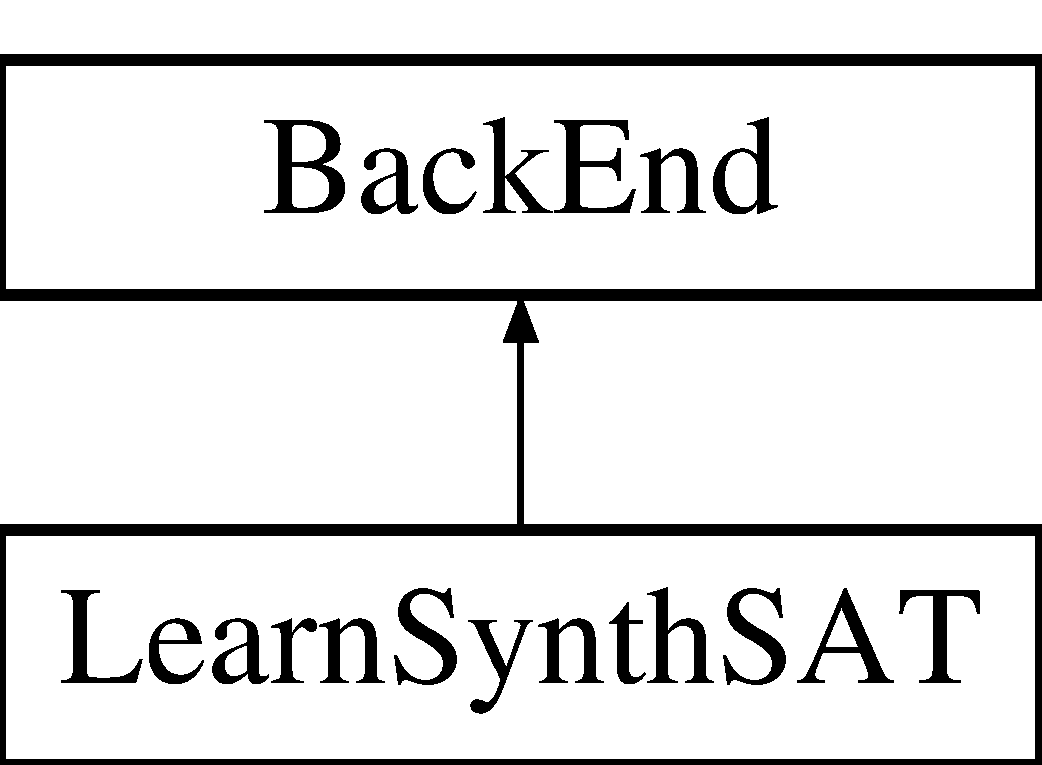
\includegraphics[height=2.000000cm]{classLearnSynthSAT}
\end{center}
\end{figure}
\subsection*{Public Member Functions}
\begin{DoxyCompactItemize}
\item 
\hyperlink{classLearnSynthSAT_a5620cd59d05720b9a148077d86efa2a8}{Learn\-Synth\-S\-A\-T} (\hyperlink{classCNFImplExtractor}{C\-N\-F\-Impl\-Extractor} $\ast$impl\-\_\-extractor)
\begin{DoxyCompactList}\small\item\em Constructor. \end{DoxyCompactList}\item 
virtual \hyperlink{classLearnSynthSAT_a2cb64f16d981276fe946d0fa0cf0bd09}{$\sim$\-Learn\-Synth\-S\-A\-T} ()
\begin{DoxyCompactList}\small\item\em Destructor. \end{DoxyCompactList}\item 
virtual bool \hyperlink{classLearnSynthSAT_a13a50b2649f44d37761fdbff26e9c0c0}{run} ()
\begin{DoxyCompactList}\small\item\em Executes this back-\/end. \end{DoxyCompactList}\end{DoxyCompactItemize}
\subsection*{Protected Member Functions}
\begin{DoxyCompactItemize}
\item 
bool \hyperlink{classLearnSynthSAT_a055b4699184d09bb7f6b15052ac684db}{compute\-Winning\-Region} ()
\begin{DoxyCompactList}\small\item\em Computes the winning region and stores the result in \hyperlink{classLearnSynthSAT_aced2bce789c7a93ed4b5391dd0690616}{winning\-\_\-region\-\_\-}. \end{DoxyCompactList}\item 
bool \hyperlink{classLearnSynthSAT_a49541a9cff8002ca31e0044ae35546a2}{compute\-Winning\-Region\-Plain} ()
\begin{DoxyCompactList}\small\item\em Uses the standard method to compute a winning region. \end{DoxyCompactList}\item 
bool \hyperlink{classLearnSynthSAT_a8727927b4e0432acb6bcea883fd2f1f9}{compute\-Winning\-Region\-Plain\-Exp} ()
\begin{DoxyCompactList}\small\item\em Like \hyperlink{classLearnSynthSAT_a49541a9cff8002ca31e0044ae35546a2}{compute\-Winning\-Region\-Plain()} but using universal expansion. \end{DoxyCompactList}\item 
bool \hyperlink{classLearnSynthSAT_a0d36fdd8180e9ba06e116b6ed3cb6a72}{compute\-Winning\-Region\-Plain\-Dep} ()
\begin{DoxyCompactList}\small\item\em Computes the winning region, exploiting temporary variables of the tran. rel. \end{DoxyCompactList}\item 
bool \hyperlink{classLearnSynthSAT_a7190dabde3f24ddb94c0484f7df3b026}{compute\-Winning\-Region\-Plain\-Dep2} ()
\begin{DoxyCompactList}\small\item\em Exploits temporary variables of the tran. rel. even more. \end{DoxyCompactList}\item 
bool \hyperlink{classLearnSynthSAT_aa981048565f10183c30c4dc0576de6b6}{compute\-Winning\-Region\-R\-G} ()
\begin{DoxyCompactList}\small\item\em Compute a winning region with optimization R\-G when generalizing counterexamples. \end{DoxyCompactList}\item 
bool \hyperlink{classLearnSynthSAT_a2a0513b4d296a1a0fd18e7d03b77b931}{compute\-Winning\-Region\-R\-G\-Exp} ()
\begin{DoxyCompactList}\small\item\em Like \hyperlink{classLearnSynthSAT_aa981048565f10183c30c4dc0576de6b6}{compute\-Winning\-Region\-R\-G()} but using universal expansion. \end{DoxyCompactList}\item 
bool \hyperlink{classLearnSynthSAT_a46b7539bdea0d37bd28bf9ac325057b7}{compute\-Winning\-Region\-R\-G\-Recy} ()
\begin{DoxyCompactList}\small\item\em Compute a winning region with optimization R\-G and U-\/clause recycling. \end{DoxyCompactList}\item 
bool \hyperlink{classLearnSynthSAT_a2d54b84ce5e87b7b2d398226faa501b0}{compute\-Winning\-Region\-R\-G\-R\-C} ()
\begin{DoxyCompactList}\small\item\em Compute a winning region with optimization R\-G and R\-C enabled. \end{DoxyCompactList}\item 
bool \hyperlink{classLearnSynthSAT_ad5683b9e004964720c8fab73fd8ac3e4}{compute\-Winning\-Region\-R\-G\-R\-C\-Exp} ()
\begin{DoxyCompactList}\small\item\em Like \hyperlink{classLearnSynthSAT_a2d54b84ce5e87b7b2d398226faa501b0}{compute\-Winning\-Region\-R\-G\-R\-C()} but using universal expansion. \end{DoxyCompactList}\item 
int \hyperlink{classLearnSynthSAT_ab7a72deebcdf330a28931720d085547d}{present\-To\-Previous} (int literal) const 
\begin{DoxyCompactList}\small\item\em Returns the previous-\/state copy of a literal. \end{DoxyCompactList}\item 
void \hyperlink{classLearnSynthSAT_a5340af48fec2799116e4271eddff6c92}{present\-To\-Previous} (vector$<$ int $>$ \&cube\-\_\-or\-\_\-clause) const 
\begin{DoxyCompactList}\small\item\em Computes the previous-\/state copy of a cube or clause. \end{DoxyCompactList}\item 
void \hyperlink{classLearnSynthSAT_a1062ed5d0994b4fb1453285811d69f53}{present\-To\-Previous} (\hyperlink{classCNF}{C\-N\-F} \&cnf) const 
\begin{DoxyCompactList}\small\item\em Computes the previous-\/state copy of a \hyperlink{classCNF}{C\-N\-F}. \end{DoxyCompactList}\item 
void \hyperlink{classLearnSynthSAT_a83be7c843ad7ffb8a15a377b2227c891}{debug\-Check\-Win\-Reg} ()
\begin{DoxyCompactList}\small\item\em Checks a winning region computed with optimization R\-C for correctness. \end{DoxyCompactList}\end{DoxyCompactItemize}
\subsection*{Protected Attributes}
\begin{DoxyCompactItemize}
\item 
\hyperlink{classLearnStatisticsSAT}{Learn\-Statistics\-S\-A\-T} \hyperlink{classLearnSynthSAT_a2175c687276e00fa0fe3e158680affc1}{statistics\-\_\-}
\begin{DoxyCompactList}\small\item\em Stores and maintains statistics and performance measures. \end{DoxyCompactList}\item 
\hyperlink{classCNF}{C\-N\-F} \hyperlink{classLearnSynthSAT_aced2bce789c7a93ed4b5391dd0690616}{winning\-\_\-region\-\_\-}
\begin{DoxyCompactList}\small\item\em The current over-\/approximation of the winning region. \end{DoxyCompactList}\item 
\hyperlink{classCNF}{C\-N\-F} \hyperlink{classLearnSynthSAT_aaa79e8772e9ce8e59dc14e3bb1784256}{winning\-\_\-region\-\_\-large\-\_\-}
\begin{DoxyCompactList}\small\item\em The current over-\/approximation of the winning region in an uncompressed form. \end{DoxyCompactList}\item 
\hyperlink{classCNF}{C\-N\-F} \hyperlink{classLearnSynthSAT_a6289a4f041ca85ce44a33143fab42888}{prev\-\_\-trans\-\_\-or\-\_\-initial\-\_\-}
\begin{DoxyCompactList}\small\item\em Says\-: the current state is initial or the previous transition relation holds. \end{DoxyCompactList}\item 
vector$<$ int $>$ \hyperlink{classLearnSynthSAT_a98f676db61a949cd9c9626e165f378a4}{current\-\_\-to\-\_\-previous\-\_\-map\-\_\-}
\begin{DoxyCompactList}\small\item\em A map from present-\/state variables to their previous-\/state copy. \end{DoxyCompactList}\item 
int \hyperlink{classLearnSynthSAT_ace0511849ad0020364743f54dd75afee}{current\-\_\-state\-\_\-is\-\_\-initial\-\_\-}
\begin{DoxyCompactList}\small\item\em A literal that is true if the current state is initial and false otherwise. \end{DoxyCompactList}\item 
\hyperlink{classCNF}{C\-N\-F} \hyperlink{classLearnSynthSAT_a1b0ed51f21b9fbb8cc0954e011968389}{different\-\_\-from\-\_\-prev\-\_\-or\-\_\-initial\-\_\-}
\begin{DoxyCompactList}\small\item\em Says\-: the current state is different from the previous one. \end{DoxyCompactList}\item 
\hyperlink{classSatSolver}{Sat\-Solver} $\ast$ \hyperlink{classLearnSynthSAT_a97e5c03d47cb7f237104472972b12c1c}{solver\-\_\-i\-\_\-}
\begin{DoxyCompactList}\small\item\em The solver for computing counterexample-\/candidates if optimization R\-C is disabled. \end{DoxyCompactList}\item 
\hyperlink{classSatSolver}{Sat\-Solver} $\ast$ \hyperlink{classLearnSynthSAT_abb28d64291205442f1df055049ef0195}{solver\-\_\-ctrl\-\_\-}
\begin{DoxyCompactList}\small\item\em The solver for checking counterexample-\/candidates. \end{DoxyCompactList}\item 
\hyperlink{classSatSolver}{Sat\-Solver} $\ast$ \hyperlink{classLearnSynthSAT_ae7f4a4e3546f46ad1256e203311226cf}{solver\-\_\-i\-\_\-ind\-\_\-}
\begin{DoxyCompactList}\small\item\em The solver for computing counterexample-\/candidates if optimization R\-C is enabled. \end{DoxyCompactList}\item 
\hyperlink{classSatSolver}{Sat\-Solver} $\ast$ \hyperlink{classLearnSynthSAT_ab81d5f53e078238feb1e948a5a5366ff}{solver\-\_\-ctrl\-\_\-ind\-\_\-}
\begin{DoxyCompactList}\small\item\em The solver for generalizing counterexamples if optimization R\-G is endabled. \end{DoxyCompactList}\item 
\hyperlink{classCNFImplExtractor}{C\-N\-F\-Impl\-Extractor} $\ast$ \hyperlink{classLearnSynthSAT_a1c7a39732a4ee3cd1ec877f2642046fc}{impl\-\_\-extractor\-\_\-}
\begin{DoxyCompactList}\small\item\em The engine to use for circuit extraction. \end{DoxyCompactList}\item 
const vector$<$ int $>$ \& \hyperlink{classLearnSynthSAT_a4892998e28f276d7b1a1b02e80799f76}{s\-\_\-}
\begin{DoxyCompactList}\small\item\em The list of present-\/state variables. \end{DoxyCompactList}\item 
const vector$<$ int $>$ \& \hyperlink{classLearnSynthSAT_ab5eac67e9f0f27b5b08f6a5e054d59c4}{i\-\_\-}
\begin{DoxyCompactList}\small\item\em The list of (uncontrollable) input variables. \end{DoxyCompactList}\item 
const vector$<$ int $>$ \& \hyperlink{classLearnSynthSAT_ad4c8ac8ca9b023a4a81fe7e3e2dcaa96}{c\-\_\-}
\begin{DoxyCompactList}\small\item\em The list of control signals (controllable input variables). \end{DoxyCompactList}\item 
const vector$<$ int $>$ \& \hyperlink{classLearnSynthSAT_a00af554fd3553881b45182300756ca0e}{n\-\_\-}
\begin{DoxyCompactList}\small\item\em The list of next-\/state variables. \end{DoxyCompactList}\item 
vector$<$ int $>$ \hyperlink{classLearnSynthSAT_a49633abdda013c437cad8f25914eeb1f}{si\-\_\-}
\begin{DoxyCompactList}\small\item\em The list of state-\/variables and input-\/variables. \end{DoxyCompactList}\item 
vector$<$ int $>$ \hyperlink{classLearnSynthSAT_af771f52e55a36e1d685aa198a1942cd8}{sic\-\_\-}
\begin{DoxyCompactList}\small\item\em The list of state-\/, input-\/, and control variables. \end{DoxyCompactList}\item 
vector$<$ int $>$ \hyperlink{classLearnSynthSAT_a2eb9ea7dbeb1eb04011e02a16fe2917d}{sicn\-\_\-}
\begin{DoxyCompactList}\small\item\em The list of state-\/, input-\/, control-\/, and next-\/state-\/variables. \end{DoxyCompactList}\end{DoxyCompactItemize}
\subsection*{Private Member Functions}
\begin{DoxyCompactItemize}
\item 
\hyperlink{classLearnSynthSAT_ae4a63ec1333eb53c2026f4e170dc12e1}{Learn\-Synth\-S\-A\-T} (const \hyperlink{classLearnSynthSAT}{Learn\-Synth\-S\-A\-T} \&other)
\begin{DoxyCompactList}\small\item\em Copy constructor. \end{DoxyCompactList}\item 
\hyperlink{classLearnSynthSAT}{Learn\-Synth\-S\-A\-T} \& \hyperlink{classLearnSynthSAT_af61b7eb7b2f4b88f358bc0d28b774293}{operator=} (const \hyperlink{classLearnSynthSAT}{Learn\-Synth\-S\-A\-T} \&other)
\begin{DoxyCompactList}\small\item\em Assignment operator. \end{DoxyCompactList}\end{DoxyCompactItemize}


\subsection{Detailed Description}
Implements a learning-\/based synthesis using two S\-A\-T solvers. 

The working principle of the algorithm implemented in this class is very similar to \hyperlink{classLearnSynthQBF}{Learn\-Synth\-Q\-B\-F}\-: We start by setting the winning region F to the set of all safe states P. In a loop, we first compute a counterexample to the correctness of this guess in form of a state from which the antagonist (controlling the uncontrollable inputs i) can enforce to leave F. The state is represented as a cube over all state-\/variables. Next, this state-\/cube is generalized into a larger region of states by dropping literals as long as the cube contains only states that are winning for the antagonist (and hence must be removed or have already been removed from F). Finally, the generalized cube is removed from F. The next iteration checks for counterexample-\/state on the refined F. This is repeated until no more counterexample-\/states exist (then the specification is realizable and F is a winning region) or the initial state has been removed from F (in which case the specification is unrealizable).

The difference to \hyperlink{classLearnSynthQBF}{Learn\-Synth\-Q\-B\-F} is that this class uses two competing S\-A\-T-\/solvers to compute a counterexample. First, solver \hyperlink{classLearnSynthSAT_a97e5c03d47cb7f237104472972b12c1c}{solver\-\_\-i\-\_\-} finds some input values i that could be chosen by the antagonist in order to leave the \hyperlink{classLearnSynthSAT_aced2bce789c7a93ed4b5391dd0690616}{winning\-\_\-region\-\_\-}. Next, \hyperlink{classLearnSynthSAT_abb28d64291205442f1df055049ef0195}{solver\-\_\-ctrl\-\_\-} checks if there exists a response of the protagonist to chose control values c such that the winning region is not left. If no such response exists, then we have found a counterexample. Otherwise, we exclude the state-\/input combination found by \hyperlink{classLearnSynthSAT_a97e5c03d47cb7f237104472972b12c1c}{solver\-\_\-i\-\_\-} (after generalizing it into a larger set of state-\/input pairs) and try again. There is also an optimization which allows to use \hyperlink{classLearnSynthSAT_a97e5c03d47cb7f237104472972b12c1c}{solver\-\_\-i\-\_\-} incrementally\-: The next state-\/copy of the winning region is updated only lazily. Also the generalization of counterexamples is implemented with a Q\-B\-F-\/solver instead of a S\-A\-T solver. Details and background can be found in the V\-M\-C\-A\-I'14 paper \char`\"{}\-S\-A\-T-\/\-Based
\-Synthesis Methods for Safety Specs\char`\"{}.

The procedure outlined above is implemented in \hyperlink{classLearnSynthSAT_a49541a9cff8002ca31e0044ae35546a2}{compute\-Winning\-Region\-Plain()}. Some variants of this procedure are implemented in other methods of this class. The method \hyperlink{classLearnSynthSAT_aa981048565f10183c30c4dc0576de6b6}{compute\-Winning\-Region\-R\-G()} also uses inductive reachability reasoning in the generalization of counterexamples, just like \hyperlink{classLearnSynthQBFInd}{Learn\-Synth\-Q\-B\-F\-Ind}. The method \hyperlink{classLearnSynthSAT_a2d54b84ce5e87b7b2d398226faa501b0}{compute\-Winning\-Region\-R\-G\-R\-C()} uses inductive reachability reasoning also during the computation or counterexamples. These extensions are described as optimization R\-G and optimization R\-C in the V\-M\-C\-A\-I'14 paper. Command-\/line parameters (--mode) decide which of these methods to use.

Finally the \hyperlink{classQBFCertImplExtractor}{Q\-B\-F\-Cert\-Impl\-Extractor} is used to extract a circuit.

\begin{DoxyAuthor}{Author}
Robert Koenighofer (\href{mailto:robert.koenighofer@iaik.tugraz.at}{\tt robert.\-koenighofer@iaik.\-tugraz.\-at}) 
\end{DoxyAuthor}
\begin{DoxyVersion}{Version}
1.\-2.\-0 
\end{DoxyVersion}


Definition at line 85 of file Learn\-Synth\-S\-A\-T.\-h.



\subsection{Constructor \& Destructor Documentation}
\hypertarget{classLearnSynthSAT_a5620cd59d05720b9a148077d86efa2a8}{\index{Learn\-Synth\-S\-A\-T@{Learn\-Synth\-S\-A\-T}!Learn\-Synth\-S\-A\-T@{Learn\-Synth\-S\-A\-T}}
\index{Learn\-Synth\-S\-A\-T@{Learn\-Synth\-S\-A\-T}!LearnSynthSAT@{Learn\-Synth\-S\-A\-T}}
\subsubsection[{Learn\-Synth\-S\-A\-T}]{\setlength{\rightskip}{0pt plus 5cm}Learn\-Synth\-S\-A\-T\-::\-Learn\-Synth\-S\-A\-T (
\begin{DoxyParamCaption}
\item[{{\bf C\-N\-F\-Impl\-Extractor} $\ast$}]{impl\-\_\-extractor}
\end{DoxyParamCaption}
)}}\label{classLearnSynthSAT_a5620cd59d05720b9a148077d86efa2a8}


Constructor. 


\begin{DoxyParams}{Parameters}
{\em impl\-\_\-extractor} & The engine to use for circuit extraction. It will be deleted by this class. \\
\hline
\end{DoxyParams}


Definition at line 43 of file Learn\-Synth\-S\-A\-T.\-cpp.



References C\-N\-F\-::add2\-Lit\-Clause(), C\-N\-F\-::add3\-Lit\-Clause(), C\-N\-F\-::add\-Clause(), c\-\_\-, Var\-Manager\-::create\-Fresh\-Prev\-Var(), Var\-Manager\-::create\-Fresh\-Tmp\-Var(), current\-\_\-state\-\_\-is\-\_\-initial\-\_\-, current\-\_\-to\-\_\-previous\-\_\-map\-\_\-, different\-\_\-from\-\_\-prev\-\_\-or\-\_\-initial\-\_\-, C\-N\-F\-::get\-Clauses(), Var\-Manager\-::get\-Max\-C\-N\-F\-Var(), A\-I\-G2\-C\-N\-F\-::get\-Trans(), Var\-Manager\-::get\-Vars\-Of\-Type(), i\-\_\-, Var\-Manager\-::instance(), A\-I\-G2\-C\-N\-F\-::instance(), n\-\_\-, present\-To\-Previous(), prev\-\_\-trans\-\_\-or\-\_\-initial\-\_\-, s\-\_\-, si\-\_\-, sic\-\_\-, sicn\-\_\-, C\-N\-F\-::swap\-With(), and Var\-Info\-::\-T\-M\-P.

\hypertarget{classLearnSynthSAT_a2cb64f16d981276fe946d0fa0cf0bd09}{\index{Learn\-Synth\-S\-A\-T@{Learn\-Synth\-S\-A\-T}!$\sim$\-Learn\-Synth\-S\-A\-T@{$\sim$\-Learn\-Synth\-S\-A\-T}}
\index{$\sim$\-Learn\-Synth\-S\-A\-T@{$\sim$\-Learn\-Synth\-S\-A\-T}!LearnSynthSAT@{Learn\-Synth\-S\-A\-T}}
\subsubsection[{$\sim$\-Learn\-Synth\-S\-A\-T}]{\setlength{\rightskip}{0pt plus 5cm}Learn\-Synth\-S\-A\-T\-::$\sim$\-Learn\-Synth\-S\-A\-T (
\begin{DoxyParamCaption}
{}
\end{DoxyParamCaption}
)\hspace{0.3cm}{\ttfamily [virtual]}}}\label{classLearnSynthSAT_a2cb64f16d981276fe946d0fa0cf0bd09}


Destructor. 



Definition at line 120 of file Learn\-Synth\-S\-A\-T.\-cpp.



References impl\-\_\-extractor\-\_\-, solver\-\_\-ctrl\-\_\-, solver\-\_\-ctrl\-\_\-ind\-\_\-, solver\-\_\-i\-\_\-, and solver\-\_\-i\-\_\-ind\-\_\-.

\hypertarget{classLearnSynthSAT_ae4a63ec1333eb53c2026f4e170dc12e1}{\index{Learn\-Synth\-S\-A\-T@{Learn\-Synth\-S\-A\-T}!Learn\-Synth\-S\-A\-T@{Learn\-Synth\-S\-A\-T}}
\index{Learn\-Synth\-S\-A\-T@{Learn\-Synth\-S\-A\-T}!LearnSynthSAT@{Learn\-Synth\-S\-A\-T}}
\subsubsection[{Learn\-Synth\-S\-A\-T}]{\setlength{\rightskip}{0pt plus 5cm}Learn\-Synth\-S\-A\-T\-::\-Learn\-Synth\-S\-A\-T (
\begin{DoxyParamCaption}
\item[{const {\bf Learn\-Synth\-S\-A\-T} \&}]{other}
\end{DoxyParamCaption}
)\hspace{0.3cm}{\ttfamily [private]}}}\label{classLearnSynthSAT_ae4a63ec1333eb53c2026f4e170dc12e1}


Copy constructor. 

The copy constructor is disabled (set private) and not implemented.


\begin{DoxyParams}{Parameters}
{\em other} & The source for creating the copy. \\
\hline
\end{DoxyParams}


\subsection{Member Function Documentation}
\hypertarget{classLearnSynthSAT_a055b4699184d09bb7f6b15052ac684db}{\index{Learn\-Synth\-S\-A\-T@{Learn\-Synth\-S\-A\-T}!compute\-Winning\-Region@{compute\-Winning\-Region}}
\index{compute\-Winning\-Region@{compute\-Winning\-Region}!LearnSynthSAT@{Learn\-Synth\-S\-A\-T}}
\subsubsection[{compute\-Winning\-Region}]{\setlength{\rightskip}{0pt plus 5cm}bool Learn\-Synth\-S\-A\-T\-::compute\-Winning\-Region (
\begin{DoxyParamCaption}
{}
\end{DoxyParamCaption}
)\hspace{0.3cm}{\ttfamily [protected]}}}\label{classLearnSynthSAT_a055b4699184d09bb7f6b15052ac684db}


Computes the winning region and stores the result in \hyperlink{classLearnSynthSAT_aced2bce789c7a93ed4b5391dd0690616}{winning\-\_\-region\-\_\-}. 

Depending on the command-\/line parameters (--mode) this method calls one of 
\begin{DoxyItemize}
\item \hyperlink{classLearnSynthSAT_a49541a9cff8002ca31e0044ae35546a2}{compute\-Winning\-Region\-Plain()} 
\item \hyperlink{classLearnSynthSAT_aa981048565f10183c30c4dc0576de6b6}{compute\-Winning\-Region\-R\-G()} 
\item \hyperlink{classLearnSynthSAT_a2d54b84ce5e87b7b2d398226faa501b0}{compute\-Winning\-Region\-R\-G\-R\-C()} 
\item \hyperlink{classLearnSynthSAT_a8727927b4e0432acb6bcea883fd2f1f9}{compute\-Winning\-Region\-Plain\-Exp()} 
\item \hyperlink{classLearnSynthSAT_a2a0513b4d296a1a0fd18e7d03b77b931}{compute\-Winning\-Region\-R\-G\-Exp()} 
\end{DoxyItemize}

\begin{DoxyReturn}{Returns}
True if the specification was realizable, false otherwise. 
\end{DoxyReturn}


Definition at line 168 of file Learn\-Synth\-S\-A\-T.\-cpp.



References compute\-Winning\-Region\-Plain(), compute\-Winning\-Region\-Plain\-Exp(), compute\-Winning\-Region\-R\-G(), compute\-Winning\-Region\-R\-G\-Exp(), compute\-Winning\-Region\-R\-G\-R\-C(), debug\-Check\-Win\-Reg(), Utils\-::debug\-Check\-Win\-Reg(), Options\-::get\-Back\-End\-Mode(), Options\-::instance(), and winning\-\_\-region\-\_\-.



Referenced by run().

\hypertarget{classLearnSynthSAT_a49541a9cff8002ca31e0044ae35546a2}{\index{Learn\-Synth\-S\-A\-T@{Learn\-Synth\-S\-A\-T}!compute\-Winning\-Region\-Plain@{compute\-Winning\-Region\-Plain}}
\index{compute\-Winning\-Region\-Plain@{compute\-Winning\-Region\-Plain}!LearnSynthSAT@{Learn\-Synth\-S\-A\-T}}
\subsubsection[{compute\-Winning\-Region\-Plain}]{\setlength{\rightskip}{0pt plus 5cm}bool Learn\-Synth\-S\-A\-T\-::compute\-Winning\-Region\-Plain (
\begin{DoxyParamCaption}
{}
\end{DoxyParamCaption}
)\hspace{0.3cm}{\ttfamily [protected]}}}\label{classLearnSynthSAT_a49541a9cff8002ca31e0044ae35546a2}


Uses the standard method to compute a winning region. 

The standard method works as described in the class description.

\begin{DoxyReturn}{Returns}
True if the specification was realizable, false otherwise. 
\end{DoxyReturn}


Definition at line 206 of file Learn\-Synth\-S\-A\-T.\-cpp.



References C\-N\-F\-::add\-Clause\-And\-Simplify(), C\-N\-F\-::add\-C\-N\-F(), c\-\_\-, C\-N\-F\-::clear(), Utils\-::compress\-State\-C\-N\-F(), Utils\-::contains\-Init(), Sat\-Solver\-::do\-Min\-Cores(), Sat\-Solver\-::do\-Rand\-Models(), Utils\-::extract(), A\-I\-G2\-C\-N\-F\-::get\-Next\-Safe\-States(), A\-I\-G2\-C\-N\-F\-::get\-Next\-Unsafe\-States(), C\-N\-F\-::get\-Nr\-Of\-Clauses(), A\-I\-G2\-C\-N\-F\-::get\-Safe\-States(), A\-I\-G2\-C\-N\-F\-::get\-Trans(), Sat\-Solver\-::inc\-Add\-Clause(), Sat\-Solver\-::inc\-Add\-C\-N\-F(), Sat\-Solver\-::inc\-Add\-Neg\-Cube\-As\-Clause(), Sat\-Solver\-::inc\-Is\-Sat\-Model\-Or\-Core(), Var\-Info\-::\-I\-N\-P\-U\-T, Var\-Manager\-::instance(), A\-I\-G2\-C\-N\-F\-::instance(), L\-\_\-\-D\-B\-G, M\-A\-S\-S\-E\-R\-T, C\-N\-F\-::negate(), Utils\-::negate\-Literals(), Learn\-Statistics\-S\-A\-T\-::notify\-After\-Check\-Candidate\-Failed(), Learn\-Statistics\-S\-A\-T\-::notify\-After\-Check\-Candidate\-Found(), Learn\-Statistics\-S\-A\-T\-::notify\-After\-Compute\-Candidate(), Learn\-Statistics\-S\-A\-T\-::notify\-After\-Refine(), Learn\-Statistics\-S\-A\-T\-::notify\-Before\-Check\-Candidate(), Learn\-Statistics\-S\-A\-T\-::notify\-Before\-Compute\-Candidate(), Learn\-Statistics\-S\-A\-T\-::notify\-Before\-Refine(), Learn\-Statistics\-S\-A\-T\-::notify\-Restart(), Var\-Info\-::\-P\-R\-E\-S\-\_\-\-S\-T\-A\-T\-E, Var\-Manager\-::reset\-To\-Last\-Push(), s\-\_\-, si\-\_\-, sic\-\_\-, sicn\-\_\-, solver\-\_\-ctrl\-\_\-, solver\-\_\-i\-\_\-, Sat\-Solver\-::start\-Incremental\-Session(), statistics\-\_\-, Utils\-::swap\-Present\-To\-Next(), C\-N\-F\-::swap\-Present\-To\-Next(), winning\-\_\-region\-\_\-, and winning\-\_\-region\-\_\-large\-\_\-.



Referenced by compute\-Winning\-Region().

\hypertarget{classLearnSynthSAT_a0d36fdd8180e9ba06e116b6ed3cb6a72}{\index{Learn\-Synth\-S\-A\-T@{Learn\-Synth\-S\-A\-T}!compute\-Winning\-Region\-Plain\-Dep@{compute\-Winning\-Region\-Plain\-Dep}}
\index{compute\-Winning\-Region\-Plain\-Dep@{compute\-Winning\-Region\-Plain\-Dep}!LearnSynthSAT@{Learn\-Synth\-S\-A\-T}}
\subsubsection[{compute\-Winning\-Region\-Plain\-Dep}]{\setlength{\rightskip}{0pt plus 5cm}bool Learn\-Synth\-S\-A\-T\-::compute\-Winning\-Region\-Plain\-Dep (
\begin{DoxyParamCaption}
{}
\end{DoxyParamCaption}
)\hspace{0.3cm}{\ttfamily [protected]}}}\label{classLearnSynthSAT_a0d36fdd8180e9ba06e116b6ed3cb6a72}


Computes the winning region, exploiting temporary variables of the tran. rel. 

\begin{DoxyNote}{Note}
This method is experimental. 
\end{DoxyNote}
\begin{DoxyReturn}{Returns}
True if the specification was realizable, false otherwise. 
\end{DoxyReturn}


Definition at line 471 of file Learn\-Synth\-S\-A\-T.\-cpp.



References C\-N\-F\-::add\-Clause\-And\-Simplify(), C\-N\-F\-::add\-C\-N\-F(), C\-N\-F\-::clear(), Utils\-::compress\-State\-C\-N\-F(), Utils\-::contains\-Init(), Var\-Info\-::\-C\-T\-R\-L, Sat\-Solver\-::do\-Min\-Cores(), Sat\-Solver\-::do\-Rand\-Models(), Utils\-::extract(), A\-I\-G2\-C\-N\-F\-::get\-Next\-Safe\-States(), A\-I\-G2\-C\-N\-F\-::get\-Next\-Unsafe\-States(), C\-N\-F\-::get\-Nr\-Of\-Clauses(), A\-I\-G2\-C\-N\-F\-::get\-Safe\-States(), A\-I\-G2\-C\-N\-F\-::get\-Tmp\-Deps\-Trans(), A\-I\-G2\-C\-N\-F\-::get\-Trans(), Var\-Manager\-::get\-Vars\-Of\-Type(), Sat\-Solver\-::inc\-Add\-Clause(), Sat\-Solver\-::inc\-Add\-C\-N\-F(), Sat\-Solver\-::inc\-Add\-Neg\-Cube\-As\-Clause(), Sat\-Solver\-::inc\-Is\-Sat\-Model\-Or\-Core(), Var\-Info\-::\-I\-N\-P\-U\-T, Var\-Manager\-::instance(), A\-I\-G2\-C\-N\-F\-::instance(), L\-\_\-\-D\-B\-G, M\-A\-S\-S\-E\-R\-T, C\-N\-F\-::negate(), Var\-Info\-::\-N\-E\-X\-T\-\_\-\-S\-T\-A\-T\-E, Learn\-Statistics\-S\-A\-T\-::notify\-After\-Check\-Candidate\-Failed(), Learn\-Statistics\-S\-A\-T\-::notify\-After\-Check\-Candidate\-Found(), Learn\-Statistics\-S\-A\-T\-::notify\-After\-Compute\-Candidate(), Learn\-Statistics\-S\-A\-T\-::notify\-After\-Refine(), Learn\-Statistics\-S\-A\-T\-::notify\-Before\-Check\-Candidate(), Learn\-Statistics\-S\-A\-T\-::notify\-Before\-Compute\-Candidate(), Learn\-Statistics\-S\-A\-T\-::notify\-Before\-Refine(), Learn\-Statistics\-S\-A\-T\-::notify\-Restart(), Var\-Info\-::\-P\-R\-E\-S\-\_\-\-S\-T\-A\-T\-E, Var\-Manager\-::reset\-To\-Last\-Push(), solver\-\_\-ctrl\-\_\-, solver\-\_\-i\-\_\-, Sat\-Solver\-::start\-Incremental\-Session(), statistics\-\_\-, Utils\-::swap\-Present\-To\-Next(), C\-N\-F\-::swap\-Present\-To\-Next(), winning\-\_\-region\-\_\-, and winning\-\_\-region\-\_\-large\-\_\-.

\hypertarget{classLearnSynthSAT_a7190dabde3f24ddb94c0484f7df3b026}{\index{Learn\-Synth\-S\-A\-T@{Learn\-Synth\-S\-A\-T}!compute\-Winning\-Region\-Plain\-Dep2@{compute\-Winning\-Region\-Plain\-Dep2}}
\index{compute\-Winning\-Region\-Plain\-Dep2@{compute\-Winning\-Region\-Plain\-Dep2}!LearnSynthSAT@{Learn\-Synth\-S\-A\-T}}
\subsubsection[{compute\-Winning\-Region\-Plain\-Dep2}]{\setlength{\rightskip}{0pt plus 5cm}bool Learn\-Synth\-S\-A\-T\-::compute\-Winning\-Region\-Plain\-Dep2 (
\begin{DoxyParamCaption}
{}
\end{DoxyParamCaption}
)\hspace{0.3cm}{\ttfamily [protected]}}}\label{classLearnSynthSAT_a7190dabde3f24ddb94c0484f7df3b026}


Exploits temporary variables of the tran. rel. even more. 

\begin{DoxyNote}{Note}
This method is experimental. 
\end{DoxyNote}
\begin{DoxyReturn}{Returns}
True if the specification was realizable, false otherwise. 
\end{DoxyReturn}


Definition at line 676 of file Learn\-Synth\-S\-A\-T.\-cpp.



References C\-N\-F\-::add\-Clause(), C\-N\-F\-::add\-Clause\-And\-Simplify(), C\-N\-F\-::add\-C\-N\-F(), C\-N\-F\-::clear(), Utils\-::compress\-State\-C\-N\-F(), Var\-Manager\-::create\-Fresh\-Tmp\-Var(), Var\-Info\-::\-C\-T\-R\-L, D\-A\-S\-S\-E\-R\-T, Sat\-Solver\-::do\-Min\-Cores(), Sat\-Solver\-::do\-Rand\-Models(), Utils\-::extract(), C\-N\-F\-::get\-Clauses(), Var\-Manager\-::get\-Max\-C\-N\-F\-Var(), A\-I\-G2\-C\-N\-F\-::get\-Next\-Safe\-States(), A\-I\-G2\-C\-N\-F\-::get\-Next\-Unsafe\-States(), C\-N\-F\-::get\-Nr\-Of\-Clauses(), A\-I\-G2\-C\-N\-F\-::get\-Safe\-States(), A\-I\-G2\-C\-N\-F\-::get\-Tmp\-Deps(), A\-I\-G2\-C\-N\-F\-::get\-Tmp\-Deps\-Trans(), A\-I\-G2\-C\-N\-F\-::get\-Trans(), Var\-Manager\-::get\-Vars\-Of\-Type(), Sat\-Solver\-::inc\-Add\-Clause(), Sat\-Solver\-::inc\-Add\-C\-N\-F(), Sat\-Solver\-::inc\-Add\-Neg\-Cube\-As\-Clause(), Sat\-Solver\-::inc\-Is\-Sat\-Model\-Or\-Core(), Var\-Info\-::\-I\-N\-P\-U\-T, Var\-Manager\-::instance(), A\-I\-G2\-C\-N\-F\-::instance(), L\-\_\-\-D\-B\-G, M\-A\-S\-S\-E\-R\-T, C\-N\-F\-::negate(), Var\-Info\-::\-N\-E\-X\-T\-\_\-\-S\-T\-A\-T\-E, Learn\-Statistics\-S\-A\-T\-::notify\-After\-Check\-Candidate\-Failed(), Learn\-Statistics\-S\-A\-T\-::notify\-After\-Check\-Candidate\-Found(), Learn\-Statistics\-S\-A\-T\-::notify\-After\-Compute\-Candidate(), Learn\-Statistics\-S\-A\-T\-::notify\-After\-Refine(), Learn\-Statistics\-S\-A\-T\-::notify\-Before\-Check\-Candidate(), Learn\-Statistics\-S\-A\-T\-::notify\-Before\-Compute\-Candidate(), Learn\-Statistics\-S\-A\-T\-::notify\-Before\-Refine(), Learn\-Statistics\-S\-A\-T\-::notify\-Restart(), Var\-Info\-::\-P\-R\-E\-S\-\_\-\-S\-T\-A\-T\-E, Var\-Manager\-::push(), C\-N\-F\-::rename\-Vars(), Var\-Manager\-::reset\-To\-Last\-Push(), solver\-\_\-ctrl\-\_\-, solver\-\_\-i\-\_\-, Sat\-Solver\-::start\-Incremental\-Session(), statistics\-\_\-, Var\-Info\-::\-T\-M\-P, winning\-\_\-region\-\_\-, and winning\-\_\-region\-\_\-large\-\_\-.

\hypertarget{classLearnSynthSAT_a8727927b4e0432acb6bcea883fd2f1f9}{\index{Learn\-Synth\-S\-A\-T@{Learn\-Synth\-S\-A\-T}!compute\-Winning\-Region\-Plain\-Exp@{compute\-Winning\-Region\-Plain\-Exp}}
\index{compute\-Winning\-Region\-Plain\-Exp@{compute\-Winning\-Region\-Plain\-Exp}!LearnSynthSAT@{Learn\-Synth\-S\-A\-T}}
\subsubsection[{compute\-Winning\-Region\-Plain\-Exp}]{\setlength{\rightskip}{0pt plus 5cm}bool Learn\-Synth\-S\-A\-T\-::compute\-Winning\-Region\-Plain\-Exp (
\begin{DoxyParamCaption}
{}
\end{DoxyParamCaption}
)\hspace{0.3cm}{\ttfamily [protected]}}}\label{classLearnSynthSAT_a8727927b4e0432acb6bcea883fd2f1f9}


Like \hyperlink{classLearnSynthSAT_a49541a9cff8002ca31e0044ae35546a2}{compute\-Winning\-Region\-Plain()} but using universal expansion. 

\begin{DoxyReturn}{Returns}
True if the specification was realizable, false otherwise. 
\end{DoxyReturn}


Definition at line 356 of file Learn\-Synth\-S\-A\-T.\-cpp.



References C\-N\-F\-::add\-Clause\-And\-Simplify(), Univ\-Expander\-::add\-Exp\-Nxt\-Clause\-To\-C(), c\-\_\-, C\-N\-F\-::clear(), Utils\-::compress\-State\-C\-N\-F(), Utils\-::contains\-Init(), Sat\-Solver\-::do\-Min\-Cores(), Sat\-Solver\-::do\-Rand\-Models(), Utils\-::extract(), C\-N\-F\-::get\-Clauses(), C\-N\-F\-::get\-Nr\-Of\-Clauses(), A\-I\-G2\-C\-N\-F\-::get\-Safe\-States(), Sat\-Solver\-::inc\-Add\-Clause(), Sat\-Solver\-::inc\-Add\-C\-N\-F(), Sat\-Solver\-::inc\-Is\-Sat\-Model\-Or\-Core(), Univ\-Expander\-::init\-Solver\-C\-Exp(), Var\-Info\-::\-I\-N\-P\-U\-T, Var\-Manager\-::instance(), A\-I\-G2\-C\-N\-F\-::instance(), L\-\_\-\-D\-B\-G, M\-A\-S\-S\-E\-R\-T, Utils\-::negate\-Literals(), Learn\-Statistics\-S\-A\-T\-::notify\-After\-Check\-Candidate\-Found(), Learn\-Statistics\-S\-A\-T\-::notify\-After\-Compute\-Candidate(), Learn\-Statistics\-S\-A\-T\-::notify\-Before\-Check\-Candidate(), Learn\-Statistics\-S\-A\-T\-::notify\-Before\-Compute\-Candidate(), Learn\-Statistics\-S\-A\-T\-::notify\-Restart(), Var\-Info\-::\-P\-R\-E\-S\-\_\-\-S\-T\-A\-T\-E, Univ\-Expander\-::reset\-Solver\-C\-Exp(), Univ\-Expander\-::reset\-Solver\-I\-Exp(), Var\-Manager\-::reset\-To\-Last\-Push(), s\-\_\-, si\-\_\-, solver\-\_\-ctrl\-\_\-, solver\-\_\-i\-\_\-, statistics\-\_\-, and winning\-\_\-region\-\_\-.



Referenced by compute\-Winning\-Region().

\hypertarget{classLearnSynthSAT_aa981048565f10183c30c4dc0576de6b6}{\index{Learn\-Synth\-S\-A\-T@{Learn\-Synth\-S\-A\-T}!compute\-Winning\-Region\-R\-G@{compute\-Winning\-Region\-R\-G}}
\index{compute\-Winning\-Region\-R\-G@{compute\-Winning\-Region\-R\-G}!LearnSynthSAT@{Learn\-Synth\-S\-A\-T}}
\subsubsection[{compute\-Winning\-Region\-R\-G}]{\setlength{\rightskip}{0pt plus 5cm}bool Learn\-Synth\-S\-A\-T\-::compute\-Winning\-Region\-R\-G (
\begin{DoxyParamCaption}
{}
\end{DoxyParamCaption}
)\hspace{0.3cm}{\ttfamily [protected]}}}\label{classLearnSynthSAT_aa981048565f10183c30c4dc0576de6b6}


Compute a winning region with optimization R\-G when generalizing counterexamples. 

Optimization R\-G is described in \hyperlink{classLearnSynthQBFInd}{Learn\-Synth\-Q\-B\-F\-Ind} already. In a nutshell, the generalization query is modified so a state that prevents generalization must be either initial or have a predecessor in F. Otherwise it is unreachable and we do not care. This means that we can remove states that are winning for the protagonist from the winning region of they are unreachable in the final implementation.

\begin{DoxyReturn}{Returns}
True if the specification was realizable, false otherwise. 
\end{DoxyReturn}


Definition at line 953 of file Learn\-Synth\-S\-A\-T.\-cpp.



References C\-N\-F\-::add\-Clause\-And\-Simplify(), C\-N\-F\-::add\-C\-N\-F(), c\-\_\-, C\-N\-F\-::clear(), Utils\-::compress\-State\-C\-N\-F(), Utils\-::contains\-Init(), current\-\_\-state\-\_\-is\-\_\-initial\-\_\-, current\-\_\-to\-\_\-previous\-\_\-map\-\_\-, Sat\-Solver\-::do\-Min\-Cores(), Sat\-Solver\-::do\-Rand\-Models(), Utils\-::extract(), Var\-Manager\-::get\-All\-Non\-Temp\-Vars(), A\-I\-G2\-C\-N\-F\-::get\-Next\-Safe\-States(), A\-I\-G2\-C\-N\-F\-::get\-Next\-Unsafe\-States(), C\-N\-F\-::get\-Nr\-Of\-Clauses(), Var\-Manager\-::get\-Pres\-Error\-State\-Var(), A\-I\-G2\-C\-N\-F\-::get\-Safe\-States(), A\-I\-G2\-C\-N\-F\-::get\-Trans(), Sat\-Solver\-::inc\-Add\-Clause(), Sat\-Solver\-::inc\-Add\-C\-N\-F(), Sat\-Solver\-::inc\-Add\-Cube(), Sat\-Solver\-::inc\-Add\-Neg\-Cube\-As\-Clause(), Sat\-Solver\-::inc\-Add\-Unit\-Clause(), Sat\-Solver\-::inc\-Is\-Sat(), Sat\-Solver\-::inc\-Is\-Sat\-Model\-Or\-Core(), Sat\-Solver\-::inc\-Pop(), Sat\-Solver\-::inc\-Push(), Var\-Info\-::\-I\-N\-P\-U\-T, Var\-Manager\-::instance(), A\-I\-G2\-C\-N\-F\-::instance(), L\-\_\-\-D\-B\-G, M\-A\-S\-S\-E\-R\-T, C\-N\-F\-::negate(), Utils\-::negate\-Literals(), Learn\-Statistics\-S\-A\-T\-::notify\-After\-Check\-Candidate\-Failed(), Learn\-Statistics\-S\-A\-T\-::notify\-After\-Check\-Candidate\-Found(), Learn\-Statistics\-S\-A\-T\-::notify\-After\-Compute\-Candidate(), Learn\-Statistics\-S\-A\-T\-::notify\-After\-Refine(), Learn\-Statistics\-S\-A\-T\-::notify\-Before\-Check\-Candidate(), Learn\-Statistics\-S\-A\-T\-::notify\-Before\-Compute\-Candidate(), Learn\-Statistics\-S\-A\-T\-::notify\-Before\-Refine(), Learn\-Statistics\-S\-A\-T\-::notify\-Restart(), Var\-Info\-::\-P\-R\-E\-S\-\_\-\-S\-T\-A\-T\-E, present\-To\-Previous(), prev\-\_\-trans\-\_\-or\-\_\-initial\-\_\-, Utils\-::remove(), Var\-Manager\-::reset\-To\-Last\-Push(), s\-\_\-, si\-\_\-, sic\-\_\-, sicn\-\_\-, solver\-\_\-ctrl\-\_\-, solver\-\_\-ctrl\-\_\-ind\-\_\-, solver\-\_\-i\-\_\-, Sat\-Solver\-::start\-Incremental\-Session(), statistics\-\_\-, Utils\-::swap\-Present\-To\-Next(), C\-N\-F\-::swap\-Present\-To\-Next(), winning\-\_\-region\-\_\-, and winning\-\_\-region\-\_\-large\-\_\-.



Referenced by compute\-Winning\-Region().

\hypertarget{classLearnSynthSAT_a2a0513b4d296a1a0fd18e7d03b77b931}{\index{Learn\-Synth\-S\-A\-T@{Learn\-Synth\-S\-A\-T}!compute\-Winning\-Region\-R\-G\-Exp@{compute\-Winning\-Region\-R\-G\-Exp}}
\index{compute\-Winning\-Region\-R\-G\-Exp@{compute\-Winning\-Region\-R\-G\-Exp}!LearnSynthSAT@{Learn\-Synth\-S\-A\-T}}
\subsubsection[{compute\-Winning\-Region\-R\-G\-Exp}]{\setlength{\rightskip}{0pt plus 5cm}bool Learn\-Synth\-S\-A\-T\-::compute\-Winning\-Region\-R\-G\-Exp (
\begin{DoxyParamCaption}
{}
\end{DoxyParamCaption}
)\hspace{0.3cm}{\ttfamily [protected]}}}\label{classLearnSynthSAT_a2a0513b4d296a1a0fd18e7d03b77b931}


Like \hyperlink{classLearnSynthSAT_aa981048565f10183c30c4dc0576de6b6}{compute\-Winning\-Region\-R\-G()} but using universal expansion. 

\begin{DoxyReturn}{Returns}
True if the specification was realizable, false otherwise. 
\end{DoxyReturn}


Definition at line 1154 of file Learn\-Synth\-S\-A\-T.\-cpp.



References C\-N\-F\-::add\-Clause\-And\-Simplify(), C\-N\-F\-::add\-C\-N\-F(), Univ\-Expander\-::add\-Exp\-Nxt\-Clause\-To\-C(), c\-\_\-, C\-N\-F\-::clear(), Utils\-::compress\-State\-C\-N\-F(), Utils\-::contains(), Utils\-::contains\-Init(), Var\-Manager\-::create\-Fresh\-Prev\-Var(), current\-\_\-state\-\_\-is\-\_\-initial\-\_\-, current\-\_\-to\-\_\-previous\-\_\-map\-\_\-, Sat\-Solver\-::do\-Min\-Cores(), Sat\-Solver\-::do\-Rand\-Models(), Utils\-::extract(), C\-N\-F\-::get\-Clauses(), A\-I\-G2\-C\-N\-F\-::get\-Next\-Unsafe\-States(), C\-N\-F\-::get\-Nr\-Of\-Clauses(), Var\-Manager\-::get\-Pres\-Error\-State\-Var(), A\-I\-G2\-C\-N\-F\-::get\-Safe\-States(), A\-I\-G2\-C\-N\-F\-::get\-Trans(), Var\-Manager\-::get\-Vars\-Of\-Type(), Sat\-Solver\-::inc\-Add2\-Lit\-Clause(), Sat\-Solver\-::inc\-Add4\-Lit\-Clause(), Sat\-Solver\-::inc\-Add\-Clause(), Sat\-Solver\-::inc\-Add\-C\-N\-F(), Sat\-Solver\-::inc\-Add\-Neg\-Cube\-As\-Clause(), Sat\-Solver\-::inc\-Add\-Unit\-Clause(), Sat\-Solver\-::inc\-Is\-Sat(), Sat\-Solver\-::inc\-Is\-Sat\-Model\-Or\-Core(), Univ\-Expander\-::init\-Solver\-C\-Exp(), Var\-Info\-::\-I\-N\-P\-U\-T, Var\-Manager\-::instance(), A\-I\-G2\-C\-N\-F\-::instance(), L\-\_\-\-D\-B\-G, L\-\_\-\-L\-O\-G, M\-A\-S\-S\-E\-R\-T, C\-N\-F\-::negate(), Utils\-::negate\-Literals(), Learn\-Statistics\-S\-A\-T\-::notify\-After\-Check\-Candidate\-Failed(), Learn\-Statistics\-S\-A\-T\-::notify\-After\-Check\-Candidate\-Found(), Learn\-Statistics\-S\-A\-T\-::notify\-After\-Compute\-Candidate(), Learn\-Statistics\-S\-A\-T\-::notify\-After\-Refine(), Learn\-Statistics\-S\-A\-T\-::notify\-Before\-Check\-Candidate(), Learn\-Statistics\-S\-A\-T\-::notify\-Before\-Compute\-Candidate(), Learn\-Statistics\-S\-A\-T\-::notify\-Before\-Refine(), Learn\-Statistics\-S\-A\-T\-::notify\-Restart(), Var\-Info\-::\-P\-R\-E\-S\-\_\-\-S\-T\-A\-T\-E, present\-To\-Previous(), Var\-Info\-::\-P\-R\-E\-V, prev\-\_\-trans\-\_\-or\-\_\-initial\-\_\-, Var\-Manager\-::push(), Utils\-::remove(), Univ\-Expander\-::reset\-Solver\-C\-Exp(), Univ\-Expander\-::reset\-Solver\-I\-Exp(), Var\-Manager\-::reset\-To\-Last\-Push(), s\-\_\-, si\-\_\-, sic\-\_\-, solver\-\_\-ctrl\-\_\-ind\-\_\-, solver\-\_\-i\-\_\-, Sat\-Solver\-::start\-Incremental\-Session(), statistics\-\_\-, C\-N\-F\-::swap\-Present\-To\-Next(), and winning\-\_\-region\-\_\-.



Referenced by compute\-Winning\-Region().

\hypertarget{classLearnSynthSAT_a2d54b84ce5e87b7b2d398226faa501b0}{\index{Learn\-Synth\-S\-A\-T@{Learn\-Synth\-S\-A\-T}!compute\-Winning\-Region\-R\-G\-R\-C@{compute\-Winning\-Region\-R\-G\-R\-C}}
\index{compute\-Winning\-Region\-R\-G\-R\-C@{compute\-Winning\-Region\-R\-G\-R\-C}!LearnSynthSAT@{Learn\-Synth\-S\-A\-T}}
\subsubsection[{compute\-Winning\-Region\-R\-G\-R\-C}]{\setlength{\rightskip}{0pt plus 5cm}bool Learn\-Synth\-S\-A\-T\-::compute\-Winning\-Region\-R\-G\-R\-C (
\begin{DoxyParamCaption}
{}
\end{DoxyParamCaption}
)\hspace{0.3cm}{\ttfamily [protected]}}}\label{classLearnSynthSAT_a2d54b84ce5e87b7b2d398226faa501b0}


Compute a winning region with optimization R\-G and R\-C enabled. 

In addition to optimization R\-G (see \hyperlink{classLearnSynthSAT_aa981048565f10183c30c4dc0576de6b6}{compute\-Winning\-Region\-R\-G()}), this method also applies optimization R\-C as described in \hyperlink{classLearnSynthQBFInd}{Learn\-Synth\-Q\-B\-F\-Ind}. In a nutshell, the queries to compute counterexamples are modified in such a way that the counterexample-\/state is either initial or has a predecessor in the current over-\/approximation of the winning region. Otherwise, the state is unreachable and can be ignored.

\begin{DoxyReturn}{Returns}
True if the specification was realizable, false otherwise. 
\end{DoxyReturn}


Definition at line 1589 of file Learn\-Synth\-S\-A\-T.\-cpp.



References C\-N\-F\-::add\-Clause\-And\-Simplify(), C\-N\-F\-::add\-C\-N\-F(), C\-N\-F\-::clear(), Utils\-::compress\-State\-C\-N\-F(), Utils\-::contains\-Init(), Var\-Info\-::\-C\-T\-R\-L, current\-\_\-state\-\_\-is\-\_\-initial\-\_\-, current\-\_\-to\-\_\-previous\-\_\-map\-\_\-, different\-\_\-from\-\_\-prev\-\_\-or\-\_\-initial\-\_\-, Sat\-Solver\-::do\-Min\-Cores(), Sat\-Solver\-::do\-Rand\-Models(), Utils\-::extract(), Var\-Manager\-::get\-All\-Non\-Temp\-Vars(), A\-I\-G2\-C\-N\-F\-::get\-Next\-Safe\-States(), A\-I\-G2\-C\-N\-F\-::get\-Next\-Unsafe\-States(), Var\-Manager\-::get\-Pres\-Error\-State\-Var(), A\-I\-G2\-C\-N\-F\-::get\-Safe\-States(), A\-I\-G2\-C\-N\-F\-::get\-Trans(), Var\-Manager\-::get\-Vars\-Of\-Type(), Sat\-Solver\-::inc\-Add\-Clause(), Sat\-Solver\-::inc\-Add\-C\-N\-F(), Sat\-Solver\-::inc\-Add\-Cube(), Sat\-Solver\-::inc\-Add\-Neg\-Cube\-As\-Clause(), Sat\-Solver\-::inc\-Add\-Unit\-Clause(), Sat\-Solver\-::inc\-Is\-Sat(), Sat\-Solver\-::inc\-Is\-Sat\-Model\-Or\-Core(), Sat\-Solver\-::inc\-Pop(), Sat\-Solver\-::inc\-Push(), Var\-Info\-::\-I\-N\-P\-U\-T, Var\-Manager\-::instance(), A\-I\-G2\-C\-N\-F\-::instance(), L\-\_\-\-D\-B\-G, M\-A\-S\-S\-E\-R\-T, C\-N\-F\-::negate(), Learn\-Statistics\-S\-A\-T\-::notify\-After\-Check\-Candidate\-Failed(), Learn\-Statistics\-S\-A\-T\-::notify\-After\-Check\-Candidate\-Found(), Learn\-Statistics\-S\-A\-T\-::notify\-After\-Compute\-Candidate(), Learn\-Statistics\-S\-A\-T\-::notify\-After\-Refine(), Learn\-Statistics\-S\-A\-T\-::notify\-Before\-Check\-Candidate(), Learn\-Statistics\-S\-A\-T\-::notify\-Before\-Compute\-Candidate(), Learn\-Statistics\-S\-A\-T\-::notify\-Before\-Refine(), Learn\-Statistics\-S\-A\-T\-::notify\-Restart(), Var\-Info\-::\-P\-R\-E\-S\-\_\-\-S\-T\-A\-T\-E, present\-To\-Previous(), prev\-\_\-trans\-\_\-or\-\_\-initial\-\_\-, Utils\-::remove(), Var\-Manager\-::reset\-To\-Last\-Push(), solver\-\_\-ctrl\-\_\-, solver\-\_\-ctrl\-\_\-ind\-\_\-, solver\-\_\-i\-\_\-, solver\-\_\-i\-\_\-ind\-\_\-, Sat\-Solver\-::start\-Incremental\-Session(), statistics\-\_\-, Utils\-::swap\-Present\-To\-Next(), C\-N\-F\-::swap\-Present\-To\-Next(), winning\-\_\-region\-\_\-, and winning\-\_\-region\-\_\-large\-\_\-.



Referenced by compute\-Winning\-Region().

\hypertarget{classLearnSynthSAT_ad5683b9e004964720c8fab73fd8ac3e4}{\index{Learn\-Synth\-S\-A\-T@{Learn\-Synth\-S\-A\-T}!compute\-Winning\-Region\-R\-G\-R\-C\-Exp@{compute\-Winning\-Region\-R\-G\-R\-C\-Exp}}
\index{compute\-Winning\-Region\-R\-G\-R\-C\-Exp@{compute\-Winning\-Region\-R\-G\-R\-C\-Exp}!LearnSynthSAT@{Learn\-Synth\-S\-A\-T}}
\subsubsection[{compute\-Winning\-Region\-R\-G\-R\-C\-Exp}]{\setlength{\rightskip}{0pt plus 5cm}bool Learn\-Synth\-S\-A\-T\-::compute\-Winning\-Region\-R\-G\-R\-C\-Exp (
\begin{DoxyParamCaption}
{}
\end{DoxyParamCaption}
)\hspace{0.3cm}{\ttfamily [protected]}}}\label{classLearnSynthSAT_ad5683b9e004964720c8fab73fd8ac3e4}


Like \hyperlink{classLearnSynthSAT_a2d54b84ce5e87b7b2d398226faa501b0}{compute\-Winning\-Region\-R\-G\-R\-C()} but using universal expansion. 

\begin{DoxyNote}{Note}
This method is experimental. 
\end{DoxyNote}
\begin{DoxyReturn}{Returns}
True if the specification was realizable, false otherwise. 
\end{DoxyReturn}


Definition at line 1802 of file Learn\-Synth\-S\-A\-T.\-cpp.



References C\-N\-F\-::add\-Clause\-And\-Simplify(), Univ\-Expander\-::add\-Exp\-Nxt\-Clause\-To\-C(), c\-\_\-, C\-N\-F\-::clear(), Utils\-::compress\-State\-C\-N\-F(), Utils\-::contains\-Init(), current\-\_\-to\-\_\-previous\-\_\-map\-\_\-, different\-\_\-from\-\_\-prev\-\_\-or\-\_\-initial\-\_\-, Sat\-Solver\-::do\-Min\-Cores(), Sat\-Solver\-::do\-Rand\-Models(), Utils\-::extract(), C\-N\-F\-::get\-Clauses(), C\-N\-F\-::get\-Nr\-Of\-Clauses(), Var\-Manager\-::get\-Pres\-Error\-State\-Var(), A\-I\-G2\-C\-N\-F\-::get\-Safe\-States(), Var\-Manager\-::get\-Vars\-Of\-Type(), Sat\-Solver\-::inc\-Add\-Clause(), Sat\-Solver\-::inc\-Add\-C\-N\-F(), Sat\-Solver\-::inc\-Add\-Unit\-Clause(), Sat\-Solver\-::inc\-Is\-Sat\-Model\-Or\-Core(), Univ\-Expander\-::init\-Solver\-C\-Exp(), Var\-Info\-::\-I\-N\-P\-U\-T, Var\-Manager\-::instance(), A\-I\-G2\-C\-N\-F\-::instance(), L\-\_\-\-D\-B\-G, M\-A\-S\-S\-E\-R\-T, Utils\-::negate\-Literals(), Learn\-Statistics\-S\-A\-T\-::notify\-After\-Check\-Candidate\-Found(), Learn\-Statistics\-S\-A\-T\-::notify\-After\-Compute\-Candidate(), Learn\-Statistics\-S\-A\-T\-::notify\-Before\-Check\-Candidate(), Learn\-Statistics\-S\-A\-T\-::notify\-Before\-Compute\-Candidate(), Learn\-Statistics\-S\-A\-T\-::notify\-Restart(), Var\-Info\-::\-P\-R\-E\-S\-\_\-\-S\-T\-A\-T\-E, present\-To\-Previous(), Var\-Info\-::\-P\-R\-E\-V, prev\-\_\-trans\-\_\-or\-\_\-initial\-\_\-, Univ\-Expander\-::reset\-Solver\-C\-Exp(), Univ\-Expander\-::reset\-Solver\-I\-Exp(), s\-\_\-, si\-\_\-, solver\-\_\-ctrl\-\_\-ind\-\_\-, solver\-\_\-i\-\_\-ind\-\_\-, statistics\-\_\-, and winning\-\_\-region\-\_\-.

\hypertarget{classLearnSynthSAT_a46b7539bdea0d37bd28bf9ac325057b7}{\index{Learn\-Synth\-S\-A\-T@{Learn\-Synth\-S\-A\-T}!compute\-Winning\-Region\-R\-G\-Recy@{compute\-Winning\-Region\-R\-G\-Recy}}
\index{compute\-Winning\-Region\-R\-G\-Recy@{compute\-Winning\-Region\-R\-G\-Recy}!LearnSynthSAT@{Learn\-Synth\-S\-A\-T}}
\subsubsection[{compute\-Winning\-Region\-R\-G\-Recy}]{\setlength{\rightskip}{0pt plus 5cm}bool Learn\-Synth\-S\-A\-T\-::compute\-Winning\-Region\-R\-G\-Recy (
\begin{DoxyParamCaption}
{}
\end{DoxyParamCaption}
)\hspace{0.3cm}{\ttfamily [protected]}}}\label{classLearnSynthSAT_a46b7539bdea0d37bd28bf9ac325057b7}


Compute a winning region with optimization R\-G and U-\/clause recycling. 

\begin{DoxyReturn}{Returns}
True if the specification was realizable, false otherwise. 
\end{DoxyReturn}


Definition at line 1380 of file Learn\-Synth\-S\-A\-T.\-cpp.



References C\-N\-F\-::add\-Clause\-And\-Simplify(), C\-N\-F\-::add\-C\-N\-F(), C\-N\-F\-::clear(), Utils\-::compress\-State\-C\-N\-F(), Utils\-::contains\-Init(), Var\-Info\-::\-C\-T\-R\-L, current\-\_\-state\-\_\-is\-\_\-initial\-\_\-, current\-\_\-to\-\_\-previous\-\_\-map\-\_\-, Sat\-Solver\-::do\-Min\-Cores(), Sat\-Solver\-::do\-Rand\-Models(), Utils\-::extract(), Var\-Manager\-::get\-All\-Non\-Temp\-Vars(), A\-I\-G2\-C\-N\-F\-::get\-Next\-Safe\-States(), A\-I\-G2\-C\-N\-F\-::get\-Next\-Unsafe\-States(), Var\-Manager\-::get\-Pres\-Error\-State\-Var(), A\-I\-G2\-C\-N\-F\-::get\-Safe\-States(), A\-I\-G2\-C\-N\-F\-::get\-Trans(), Var\-Manager\-::get\-Vars\-Of\-Type(), Sat\-Solver\-::inc\-Add\-Clause(), Sat\-Solver\-::inc\-Add\-C\-N\-F(), Sat\-Solver\-::inc\-Add\-Cube(), Sat\-Solver\-::inc\-Add\-Neg\-Cube\-As\-Clause(), Sat\-Solver\-::inc\-Add\-Unit\-Clause(), Sat\-Solver\-::inc\-Is\-Sat(), Sat\-Solver\-::inc\-Is\-Sat\-Model\-Or\-Core(), Sat\-Solver\-::inc\-Pop(), Sat\-Solver\-::inc\-Push(), Var\-Info\-::\-I\-N\-P\-U\-T, Var\-Manager\-::instance(), A\-I\-G2\-C\-N\-F\-::instance(), C\-N\-F\-::is\-Sat\-By(), L\-\_\-\-D\-B\-G, M\-A\-S\-S\-E\-R\-T, C\-N\-F\-::negate(), Learn\-Statistics\-S\-A\-T\-::notify\-After\-Check\-Candidate\-Failed(), Learn\-Statistics\-S\-A\-T\-::notify\-After\-Check\-Candidate\-Found(), Learn\-Statistics\-S\-A\-T\-::notify\-After\-Compute\-Candidate(), Learn\-Statistics\-S\-A\-T\-::notify\-After\-Refine(), Learn\-Statistics\-S\-A\-T\-::notify\-Before\-Check\-Candidate(), Learn\-Statistics\-S\-A\-T\-::notify\-Before\-Compute\-Candidate(), Learn\-Statistics\-S\-A\-T\-::notify\-Before\-Refine(), Learn\-Statistics\-S\-A\-T\-::notify\-Restart(), Var\-Info\-::\-P\-R\-E\-S\-\_\-\-S\-T\-A\-T\-E, present\-To\-Previous(), prev\-\_\-trans\-\_\-or\-\_\-initial\-\_\-, Utils\-::remove(), Var\-Manager\-::reset\-To\-Last\-Push(), solver\-\_\-ctrl\-\_\-, solver\-\_\-ctrl\-\_\-ind\-\_\-, solver\-\_\-i\-\_\-, Sat\-Solver\-::start\-Incremental\-Session(), statistics\-\_\-, Utils\-::swap\-Present\-To\-Next(), C\-N\-F\-::swap\-Present\-To\-Next(), winning\-\_\-region\-\_\-, and winning\-\_\-region\-\_\-large\-\_\-.

\hypertarget{classLearnSynthSAT_a83be7c843ad7ffb8a15a377b2227c891}{\index{Learn\-Synth\-S\-A\-T@{Learn\-Synth\-S\-A\-T}!debug\-Check\-Win\-Reg@{debug\-Check\-Win\-Reg}}
\index{debug\-Check\-Win\-Reg@{debug\-Check\-Win\-Reg}!LearnSynthSAT@{Learn\-Synth\-S\-A\-T}}
\subsubsection[{debug\-Check\-Win\-Reg}]{\setlength{\rightskip}{0pt plus 5cm}void Learn\-Synth\-S\-A\-T\-::debug\-Check\-Win\-Reg (
\begin{DoxyParamCaption}
{}
\end{DoxyParamCaption}
)\hspace{0.3cm}{\ttfamily [protected]}}}\label{classLearnSynthSAT_a83be7c843ad7ffb8a15a377b2227c891}


Checks a winning region computed with optimization R\-C for correctness. 

We usually check the correctness of the winning region in debug-\/mode by calling \hyperlink{classUtils_acc29602987b73022546a6d752a7e093f}{Utils\-::debug\-Check\-Win\-Reg()}. However, this method of \hyperlink{classUtils}{Utils} does not work for winning regions that have been computed with optimization R\-C enabled. In such cases we this method. 

Definition at line 1981 of file Learn\-Synth\-S\-A\-T.\-cpp.



References Q\-B\-F\-Solver\-::\-A, C\-N\-F\-::add\-C\-N\-F(), C\-N\-F\-::clear(), Var\-Info\-::\-C\-T\-R\-L, different\-\_\-from\-\_\-prev\-\_\-or\-\_\-initial\-\_\-, Q\-B\-F\-Solver\-::\-E, Var\-Info\-::\-I\-N\-P\-U\-T, A\-I\-G2\-C\-N\-F\-::instance(), Dep\-Q\-B\-F\-Api\-::is\-Sat(), Lingeling\-Api\-::is\-Sat(), L\-\_\-\-D\-B\-G, M\-A\-S\-S\-E\-R\-T, C\-N\-F\-::negate(), Var\-Info\-::\-N\-E\-X\-T\-\_\-\-S\-T\-A\-T\-E, Var\-Info\-::\-P\-R\-E\-S\-\_\-\-S\-T\-A\-T\-E, present\-To\-Previous(), Var\-Info\-::\-P\-R\-E\-V, prev\-\_\-trans\-\_\-or\-\_\-initial\-\_\-, C\-N\-F\-::swap\-Present\-To\-Next(), Var\-Info\-::\-T\-M\-P, and winning\-\_\-region\-\_\-.



Referenced by compute\-Winning\-Region().

\hypertarget{classLearnSynthSAT_af61b7eb7b2f4b88f358bc0d28b774293}{\index{Learn\-Synth\-S\-A\-T@{Learn\-Synth\-S\-A\-T}!operator=@{operator=}}
\index{operator=@{operator=}!LearnSynthSAT@{Learn\-Synth\-S\-A\-T}}
\subsubsection[{operator=}]{\setlength{\rightskip}{0pt plus 5cm}{\bf Learn\-Synth\-S\-A\-T}\& Learn\-Synth\-S\-A\-T\-::operator= (
\begin{DoxyParamCaption}
\item[{const {\bf Learn\-Synth\-S\-A\-T} \&}]{other}
\end{DoxyParamCaption}
)\hspace{0.3cm}{\ttfamily [private]}}}\label{classLearnSynthSAT_af61b7eb7b2f4b88f358bc0d28b774293}


Assignment operator. 

The assignment operator is disabled (set private) and not implemented.


\begin{DoxyParams}{Parameters}
{\em other} & The source for creating the copy. \\
\hline
\end{DoxyParams}
\begin{DoxyReturn}{Returns}
The result of the assignment, i.\-e, $\ast$this. 
\end{DoxyReturn}
\hypertarget{classLearnSynthSAT_ab7a72deebcdf330a28931720d085547d}{\index{Learn\-Synth\-S\-A\-T@{Learn\-Synth\-S\-A\-T}!present\-To\-Previous@{present\-To\-Previous}}
\index{present\-To\-Previous@{present\-To\-Previous}!LearnSynthSAT@{Learn\-Synth\-S\-A\-T}}
\subsubsection[{present\-To\-Previous}]{\setlength{\rightskip}{0pt plus 5cm}int Learn\-Synth\-S\-A\-T\-::present\-To\-Previous (
\begin{DoxyParamCaption}
\item[{int}]{literal}
\end{DoxyParamCaption}
) const\hspace{0.3cm}{\ttfamily [protected]}}}\label{classLearnSynthSAT_ab7a72deebcdf330a28931720d085547d}


Returns the previous-\/state copy of a literal. 


\begin{DoxyParams}{Parameters}
{\em literal} & The literal to transform. \\
\hline
\end{DoxyParams}
\begin{DoxyReturn}{Returns}
The previous-\/state copy of a literal. 
\end{DoxyReturn}


Definition at line 1951 of file Learn\-Synth\-S\-A\-T.\-cpp.



References current\-\_\-to\-\_\-previous\-\_\-map\-\_\-.



Referenced by compute\-Winning\-Region\-R\-G(), compute\-Winning\-Region\-R\-G\-Exp(), compute\-Winning\-Region\-R\-G\-R\-C(), compute\-Winning\-Region\-R\-G\-R\-C\-Exp(), compute\-Winning\-Region\-R\-G\-Recy(), debug\-Check\-Win\-Reg(), Learn\-Synth\-S\-A\-T(), and present\-To\-Previous().

\hypertarget{classLearnSynthSAT_a5340af48fec2799116e4271eddff6c92}{\index{Learn\-Synth\-S\-A\-T@{Learn\-Synth\-S\-A\-T}!present\-To\-Previous@{present\-To\-Previous}}
\index{present\-To\-Previous@{present\-To\-Previous}!LearnSynthSAT@{Learn\-Synth\-S\-A\-T}}
\subsubsection[{present\-To\-Previous}]{\setlength{\rightskip}{0pt plus 5cm}void Learn\-Synth\-S\-A\-T\-::present\-To\-Previous (
\begin{DoxyParamCaption}
\item[{vector$<$ int $>$ \&}]{cube\-\_\-or\-\_\-clause}
\end{DoxyParamCaption}
) const\hspace{0.3cm}{\ttfamily [protected]}}}\label{classLearnSynthSAT_a5340af48fec2799116e4271eddff6c92}


Computes the previous-\/state copy of a cube or clause. 


\begin{DoxyParams}{Parameters}
{\em cube\-\_\-or\-\_\-clause} & A cube or clause (in form of a vector of literals) over the present state variables. This vector is overwritten by the corresponding cube of clause over the previous-\/state literals (i.\-e., all literals are replaced by their previous-\/state copy). \\
\hline
\end{DoxyParams}


Definition at line 1961 of file Learn\-Synth\-S\-A\-T.\-cpp.



References present\-To\-Previous().

\hypertarget{classLearnSynthSAT_a1062ed5d0994b4fb1453285811d69f53}{\index{Learn\-Synth\-S\-A\-T@{Learn\-Synth\-S\-A\-T}!present\-To\-Previous@{present\-To\-Previous}}
\index{present\-To\-Previous@{present\-To\-Previous}!LearnSynthSAT@{Learn\-Synth\-S\-A\-T}}
\subsubsection[{present\-To\-Previous}]{\setlength{\rightskip}{0pt plus 5cm}void Learn\-Synth\-S\-A\-T\-::present\-To\-Previous (
\begin{DoxyParamCaption}
\item[{{\bf C\-N\-F} \&}]{cnf}
\end{DoxyParamCaption}
) const\hspace{0.3cm}{\ttfamily [protected]}}}\label{classLearnSynthSAT_a1062ed5d0994b4fb1453285811d69f53}


Computes the previous-\/state copy of a \hyperlink{classCNF}{C\-N\-F}. 


\begin{DoxyParams}{Parameters}
{\em cnf} & A \hyperlink{classCNF}{C\-N\-F} formula over the present state variables. This \hyperlink{classCNF}{C\-N\-F} is overwritten by the corresponding \hyperlink{classCNF}{C\-N\-F} over the previous-\/state literals (i.\-e., all literals are replaced by their previous-\/state copy). \\
\hline
\end{DoxyParams}


Definition at line 1968 of file Learn\-Synth\-S\-A\-T.\-cpp.



References C\-N\-F\-::add\-Clause(), C\-N\-F\-::clear(), C\-N\-F\-::get\-Clauses(), and present\-To\-Previous().

\hypertarget{classLearnSynthSAT_a13a50b2649f44d37761fdbff26e9c0c0}{\index{Learn\-Synth\-S\-A\-T@{Learn\-Synth\-S\-A\-T}!run@{run}}
\index{run@{run}!LearnSynthSAT@{Learn\-Synth\-S\-A\-T}}
\subsubsection[{run}]{\setlength{\rightskip}{0pt plus 5cm}bool Learn\-Synth\-S\-A\-T\-::run (
\begin{DoxyParamCaption}
{}
\end{DoxyParamCaption}
)\hspace{0.3cm}{\ttfamily [virtual]}}}\label{classLearnSynthSAT_a13a50b2649f44d37761fdbff26e9c0c0}


Executes this back-\/end. 

The working principle of this method is very similar to \hyperlink{classLearnSynthQBF_aed85bb2fe317a5fdc7eef71fe598c606}{Learn\-Synth\-Q\-B\-F\-::run()}\-: We start by setting the winning region F to the set of all safe states P. In a loop, we first compute a counterexample to the correctness of this guess in form of a state from which the antagonist (controlling the uncontrollable inputs i) can enforce to leave F. The state is represented as a cube over all state-\/variables. Next, this state-\/cube is generalized into a larger region of states by dropping literals as long as the cube contains only states that are winning for the antagonist (and hence must be removed or have already been removed from F). Finally, the generalized cube is removed from F. The next iteration checks for counterexample-\/state on the refined F. This is repeated until no more counterexample-\/states exist (then the specification is realizable and F is a winning region) or the initial state has been removed from F (in which case the specification is unrealizable). The difference to \hyperlink{classLearnSynthQBF}{Learn\-Synth\-Q\-B\-F} is that this method uses two competing S\-A\-T-\/solvers to compute a counterexample. First, solver \hyperlink{classLearnSynthSAT_a97e5c03d47cb7f237104472972b12c1c}{solver\-\_\-i\-\_\-} finds some input values i that could be chosen by the antagonist in order to leave the \hyperlink{classLearnSynthSAT_aced2bce789c7a93ed4b5391dd0690616}{winning\-\_\-region\-\_\-}. Next, \hyperlink{classLearnSynthSAT_abb28d64291205442f1df055049ef0195}{solver\-\_\-ctrl\-\_\-} checks if there exists a response of the protagonist to chose control values c such that the winning region is not left. If no such response exists, then we have found a counterexample. Otherwise, we exclude the state-\/input combination found by \hyperlink{classLearnSynthSAT_a97e5c03d47cb7f237104472972b12c1c}{solver\-\_\-i\-\_\-} (after generalizing it into a larger set of state-\/input pairs) and try again. There is also an optimization which allows to use \hyperlink{classLearnSynthSAT_a97e5c03d47cb7f237104472972b12c1c}{solver\-\_\-i\-\_\-} incrementally\-: The next state-\/copy of the winning region is updated only lazily. Also the generalization of counterexamples is implemented with a Q\-B\-F-\/solver instead of a S\-A\-T solver. Details and background can be found in the V\-M\-C\-A\-I'14 paper \char`\"{}\-S\-A\-T-\/\-Based
\-Synthesis Methods for Safety Specs\char`\"{}.

Command-\/line parameters (--mode) are used to select different variants of this method. There is 
\begin{DoxyItemize}
\item the standard method as described above, 
\item a variant which uses inductive reachability reasoning in the generalization of counterexamples, just like \hyperlink{classLearnSynthQBFInd}{Learn\-Synth\-Q\-B\-F\-Ind} (optimization 'R\-G') 
\item a variant which uses inductive reachability reasoning also in the computation of counterexamples, just like \hyperlink{classLearnSynthQBFInd}{Learn\-Synth\-Q\-B\-F\-Ind} (optimization 'R\-G' and 'R\-C') 
\item the standard method, but performing universal expansion on certain variables in order to reduce the number of iterations 
\item the standard method with optimization R\-G and a universal expansion on certain variables in order to reduce the number of iterations 
\end{DoxyItemize}

\begin{DoxyReturn}{Returns}
True if the specification was realizable, false otherwise. 
\end{DoxyReturn}


Implements \hyperlink{classBackEnd_a099e717dc71e9cc2d838b1ca86340590}{Back\-End}.



Definition at line 135 of file Learn\-Synth\-S\-A\-T.\-cpp.



References compute\-Winning\-Region(), C\-N\-F\-Impl\-Extractor\-::extract\-Circuit(), impl\-\_\-extractor\-\_\-, Var\-Manager\-::instance(), Options\-::instance(), L\-\_\-\-I\-N\-F, L\-\_\-\-R\-E\-S, C\-N\-F\-Impl\-Extractor\-::log\-Statistics(), Learn\-Statistics\-S\-A\-T\-::log\-Statistics(), M\-A\-S\-S\-E\-R\-T, Learn\-Statistics\-S\-A\-T\-::notify\-Win\-Reg\-End(), Learn\-Statistics\-S\-A\-T\-::notify\-Win\-Reg\-Start(), Var\-Manager\-::push(), statistics\-\_\-, and winning\-\_\-region\-\_\-.



\subsection{Member Data Documentation}
\hypertarget{classLearnSynthSAT_ad4c8ac8ca9b023a4a81fe7e3e2dcaa96}{\index{Learn\-Synth\-S\-A\-T@{Learn\-Synth\-S\-A\-T}!c\-\_\-@{c\-\_\-}}
\index{c\-\_\-@{c\-\_\-}!LearnSynthSAT@{Learn\-Synth\-S\-A\-T}}
\subsubsection[{c\-\_\-}]{\setlength{\rightskip}{0pt plus 5cm}const vector$<$int$>$\& Learn\-Synth\-S\-A\-T\-::c\-\_\-\hspace{0.3cm}{\ttfamily [protected]}}}\label{classLearnSynthSAT_ad4c8ac8ca9b023a4a81fe7e3e2dcaa96}


The list of control signals (controllable input variables). 

This list is often used, so we keep it as a field to increase readability of the code. 

Definition at line 385 of file Learn\-Synth\-S\-A\-T.\-h.



Referenced by compute\-Winning\-Region\-Plain(), compute\-Winning\-Region\-Plain\-Exp(), compute\-Winning\-Region\-R\-G(), compute\-Winning\-Region\-R\-G\-Exp(), compute\-Winning\-Region\-R\-G\-R\-C\-Exp(), and Learn\-Synth\-S\-A\-T().

\hypertarget{classLearnSynthSAT_ace0511849ad0020364743f54dd75afee}{\index{Learn\-Synth\-S\-A\-T@{Learn\-Synth\-S\-A\-T}!current\-\_\-state\-\_\-is\-\_\-initial\-\_\-@{current\-\_\-state\-\_\-is\-\_\-initial\-\_\-}}
\index{current\-\_\-state\-\_\-is\-\_\-initial\-\_\-@{current\-\_\-state\-\_\-is\-\_\-initial\-\_\-}!LearnSynthSAT@{Learn\-Synth\-S\-A\-T}}
\subsubsection[{current\-\_\-state\-\_\-is\-\_\-initial\-\_\-}]{\setlength{\rightskip}{0pt plus 5cm}int Learn\-Synth\-S\-A\-T\-::current\-\_\-state\-\_\-is\-\_\-initial\-\_\-\hspace{0.3cm}{\ttfamily [protected]}}}\label{classLearnSynthSAT_ace0511849ad0020364743f54dd75afee}


A literal that is true if the current state is initial and false otherwise. 

The clauses assigning the literal are part of \hyperlink{classLearnSynthSAT_a6289a4f041ca85ce44a33143fab42888}{prev\-\_\-trans\-\_\-or\-\_\-initial\-\_\-}. 

Definition at line 326 of file Learn\-Synth\-S\-A\-T.\-h.



Referenced by compute\-Winning\-Region\-R\-G(), compute\-Winning\-Region\-R\-G\-Exp(), compute\-Winning\-Region\-R\-G\-R\-C(), compute\-Winning\-Region\-R\-G\-Recy(), and Learn\-Synth\-S\-A\-T().

\hypertarget{classLearnSynthSAT_a98f676db61a949cd9c9626e165f378a4}{\index{Learn\-Synth\-S\-A\-T@{Learn\-Synth\-S\-A\-T}!current\-\_\-to\-\_\-previous\-\_\-map\-\_\-@{current\-\_\-to\-\_\-previous\-\_\-map\-\_\-}}
\index{current\-\_\-to\-\_\-previous\-\_\-map\-\_\-@{current\-\_\-to\-\_\-previous\-\_\-map\-\_\-}!LearnSynthSAT@{Learn\-Synth\-S\-A\-T}}
\subsubsection[{current\-\_\-to\-\_\-previous\-\_\-map\-\_\-}]{\setlength{\rightskip}{0pt plus 5cm}vector$<$int$>$ Learn\-Synth\-S\-A\-T\-::current\-\_\-to\-\_\-previous\-\_\-map\-\_\-\hspace{0.3cm}{\ttfamily [protected]}}}\label{classLearnSynthSAT_a98f676db61a949cd9c9626e165f378a4}


A map from present-\/state variables to their previous-\/state copy. 



Definition at line 319 of file Learn\-Synth\-S\-A\-T.\-h.



Referenced by compute\-Winning\-Region\-R\-G(), compute\-Winning\-Region\-R\-G\-Exp(), compute\-Winning\-Region\-R\-G\-R\-C(), compute\-Winning\-Region\-R\-G\-R\-C\-Exp(), compute\-Winning\-Region\-R\-G\-Recy(), Learn\-Synth\-S\-A\-T(), and present\-To\-Previous().

\hypertarget{classLearnSynthSAT_a1b0ed51f21b9fbb8cc0954e011968389}{\index{Learn\-Synth\-S\-A\-T@{Learn\-Synth\-S\-A\-T}!different\-\_\-from\-\_\-prev\-\_\-or\-\_\-initial\-\_\-@{different\-\_\-from\-\_\-prev\-\_\-or\-\_\-initial\-\_\-}}
\index{different\-\_\-from\-\_\-prev\-\_\-or\-\_\-initial\-\_\-@{different\-\_\-from\-\_\-prev\-\_\-or\-\_\-initial\-\_\-}!LearnSynthSAT@{Learn\-Synth\-S\-A\-T}}
\subsubsection[{different\-\_\-from\-\_\-prev\-\_\-or\-\_\-initial\-\_\-}]{\setlength{\rightskip}{0pt plus 5cm}{\bf C\-N\-F} Learn\-Synth\-S\-A\-T\-::different\-\_\-from\-\_\-prev\-\_\-or\-\_\-initial\-\_\-\hspace{0.3cm}{\ttfamily [protected]}}}\label{classLearnSynthSAT_a1b0ed51f21b9fbb8cc0954e011968389}


Says\-: the current state is different from the previous one. 

This \hyperlink{classCNF}{C\-N\-F} expresses that the current state is different from the previous state. This is an important building block for the \hyperlink{classCNF}{C\-N\-F} to compute counterexamples if optimization R\-C is enabled. 

Definition at line 335 of file Learn\-Synth\-S\-A\-T.\-h.



Referenced by compute\-Winning\-Region\-R\-G\-R\-C(), compute\-Winning\-Region\-R\-G\-R\-C\-Exp(), debug\-Check\-Win\-Reg(), and Learn\-Synth\-S\-A\-T().

\hypertarget{classLearnSynthSAT_ab5eac67e9f0f27b5b08f6a5e054d59c4}{\index{Learn\-Synth\-S\-A\-T@{Learn\-Synth\-S\-A\-T}!i\-\_\-@{i\-\_\-}}
\index{i\-\_\-@{i\-\_\-}!LearnSynthSAT@{Learn\-Synth\-S\-A\-T}}
\subsubsection[{i\-\_\-}]{\setlength{\rightskip}{0pt plus 5cm}const vector$<$int$>$\& Learn\-Synth\-S\-A\-T\-::i\-\_\-\hspace{0.3cm}{\ttfamily [protected]}}}\label{classLearnSynthSAT_ab5eac67e9f0f27b5b08f6a5e054d59c4}


The list of (uncontrollable) input variables. 

This list is often used, so we keep it as a field to increase readability of the code. 

Definition at line 378 of file Learn\-Synth\-S\-A\-T.\-h.



Referenced by Learn\-Synth\-S\-A\-T().

\hypertarget{classLearnSynthSAT_a1c7a39732a4ee3cd1ec877f2642046fc}{\index{Learn\-Synth\-S\-A\-T@{Learn\-Synth\-S\-A\-T}!impl\-\_\-extractor\-\_\-@{impl\-\_\-extractor\-\_\-}}
\index{impl\-\_\-extractor\-\_\-@{impl\-\_\-extractor\-\_\-}!LearnSynthSAT@{Learn\-Synth\-S\-A\-T}}
\subsubsection[{impl\-\_\-extractor\-\_\-}]{\setlength{\rightskip}{0pt plus 5cm}{\bf C\-N\-F\-Impl\-Extractor}$\ast$ Learn\-Synth\-S\-A\-T\-::impl\-\_\-extractor\-\_\-\hspace{0.3cm}{\ttfamily [protected]}}}\label{classLearnSynthSAT_a1c7a39732a4ee3cd1ec877f2642046fc}


The engine to use for circuit extraction. 

It will be deleted by this class (in the destructor). 

Definition at line 364 of file Learn\-Synth\-S\-A\-T.\-h.



Referenced by run(), and $\sim$\-Learn\-Synth\-S\-A\-T().

\hypertarget{classLearnSynthSAT_a00af554fd3553881b45182300756ca0e}{\index{Learn\-Synth\-S\-A\-T@{Learn\-Synth\-S\-A\-T}!n\-\_\-@{n\-\_\-}}
\index{n\-\_\-@{n\-\_\-}!LearnSynthSAT@{Learn\-Synth\-S\-A\-T}}
\subsubsection[{n\-\_\-}]{\setlength{\rightskip}{0pt plus 5cm}const vector$<$int$>$\& Learn\-Synth\-S\-A\-T\-::n\-\_\-\hspace{0.3cm}{\ttfamily [protected]}}}\label{classLearnSynthSAT_a00af554fd3553881b45182300756ca0e}


The list of next-\/state variables. 

This list is often used, so we keep it as a field to increase readability of the code. 

Definition at line 392 of file Learn\-Synth\-S\-A\-T.\-h.



Referenced by Learn\-Synth\-S\-A\-T().

\hypertarget{classLearnSynthSAT_a6289a4f041ca85ce44a33143fab42888}{\index{Learn\-Synth\-S\-A\-T@{Learn\-Synth\-S\-A\-T}!prev\-\_\-trans\-\_\-or\-\_\-initial\-\_\-@{prev\-\_\-trans\-\_\-or\-\_\-initial\-\_\-}}
\index{prev\-\_\-trans\-\_\-or\-\_\-initial\-\_\-@{prev\-\_\-trans\-\_\-or\-\_\-initial\-\_\-}!LearnSynthSAT@{Learn\-Synth\-S\-A\-T}}
\subsubsection[{prev\-\_\-trans\-\_\-or\-\_\-initial\-\_\-}]{\setlength{\rightskip}{0pt plus 5cm}{\bf C\-N\-F} Learn\-Synth\-S\-A\-T\-::prev\-\_\-trans\-\_\-or\-\_\-initial\-\_\-\hspace{0.3cm}{\ttfamily [protected]}}}\label{classLearnSynthSAT_a6289a4f041ca85ce44a33143fab42888}


Says\-: the current state is initial or the previous transition relation holds. 

This \hyperlink{classCNF}{C\-N\-F} expresses that the current state is initial or the previous-\/state copy of the transition relation holds. This is an important building block for the \hyperlink{classCNF}{C\-N\-F} to compute or generalize counterexamples if optimization R\-G or R\-C is enabled. 

Definition at line 314 of file Learn\-Synth\-S\-A\-T.\-h.



Referenced by compute\-Winning\-Region\-R\-G(), compute\-Winning\-Region\-R\-G\-Exp(), compute\-Winning\-Region\-R\-G\-R\-C(), compute\-Winning\-Region\-R\-G\-R\-C\-Exp(), compute\-Winning\-Region\-R\-G\-Recy(), debug\-Check\-Win\-Reg(), and Learn\-Synth\-S\-A\-T().

\hypertarget{classLearnSynthSAT_a4892998e28f276d7b1a1b02e80799f76}{\index{Learn\-Synth\-S\-A\-T@{Learn\-Synth\-S\-A\-T}!s\-\_\-@{s\-\_\-}}
\index{s\-\_\-@{s\-\_\-}!LearnSynthSAT@{Learn\-Synth\-S\-A\-T}}
\subsubsection[{s\-\_\-}]{\setlength{\rightskip}{0pt plus 5cm}const vector$<$int$>$\& Learn\-Synth\-S\-A\-T\-::s\-\_\-\hspace{0.3cm}{\ttfamily [protected]}}}\label{classLearnSynthSAT_a4892998e28f276d7b1a1b02e80799f76}


The list of present-\/state variables. 

This list is often used, so we keep it as a field to increase readability of the code. 

Definition at line 371 of file Learn\-Synth\-S\-A\-T.\-h.



Referenced by compute\-Winning\-Region\-Plain(), compute\-Winning\-Region\-Plain\-Exp(), compute\-Winning\-Region\-R\-G(), compute\-Winning\-Region\-R\-G\-Exp(), compute\-Winning\-Region\-R\-G\-R\-C\-Exp(), and Learn\-Synth\-S\-A\-T().

\hypertarget{classLearnSynthSAT_a49633abdda013c437cad8f25914eeb1f}{\index{Learn\-Synth\-S\-A\-T@{Learn\-Synth\-S\-A\-T}!si\-\_\-@{si\-\_\-}}
\index{si\-\_\-@{si\-\_\-}!LearnSynthSAT@{Learn\-Synth\-S\-A\-T}}
\subsubsection[{si\-\_\-}]{\setlength{\rightskip}{0pt plus 5cm}vector$<$int$>$ Learn\-Synth\-S\-A\-T\-::si\-\_\-\hspace{0.3cm}{\ttfamily [protected]}}}\label{classLearnSynthSAT_a49633abdda013c437cad8f25914eeb1f}


The list of state-\/variables and input-\/variables. 

This vector contains the \hyperlink{classCNF}{C\-N\-F} version of the state variables and the uncontrollable input variables. This vector of variables is used often, and thus stored here as a field. 

Definition at line 400 of file Learn\-Synth\-S\-A\-T.\-h.



Referenced by compute\-Winning\-Region\-Plain(), compute\-Winning\-Region\-Plain\-Exp(), compute\-Winning\-Region\-R\-G(), compute\-Winning\-Region\-R\-G\-Exp(), compute\-Winning\-Region\-R\-G\-R\-C\-Exp(), and Learn\-Synth\-S\-A\-T().

\hypertarget{classLearnSynthSAT_af771f52e55a36e1d685aa198a1942cd8}{\index{Learn\-Synth\-S\-A\-T@{Learn\-Synth\-S\-A\-T}!sic\-\_\-@{sic\-\_\-}}
\index{sic\-\_\-@{sic\-\_\-}!LearnSynthSAT@{Learn\-Synth\-S\-A\-T}}
\subsubsection[{sic\-\_\-}]{\setlength{\rightskip}{0pt plus 5cm}vector$<$int$>$ Learn\-Synth\-S\-A\-T\-::sic\-\_\-\hspace{0.3cm}{\ttfamily [protected]}}}\label{classLearnSynthSAT_af771f52e55a36e1d685aa198a1942cd8}


The list of state-\/, input-\/, and control variables. 

This vector contains the \hyperlink{classCNF}{C\-N\-F} version of the state variables, the uncontrollable input variables, and the controllable input variables. This vector of variables is used often, and thus stored here as a field. 

Definition at line 409 of file Learn\-Synth\-S\-A\-T.\-h.



Referenced by compute\-Winning\-Region\-Plain(), compute\-Winning\-Region\-R\-G(), compute\-Winning\-Region\-R\-G\-Exp(), and Learn\-Synth\-S\-A\-T().

\hypertarget{classLearnSynthSAT_a2eb9ea7dbeb1eb04011e02a16fe2917d}{\index{Learn\-Synth\-S\-A\-T@{Learn\-Synth\-S\-A\-T}!sicn\-\_\-@{sicn\-\_\-}}
\index{sicn\-\_\-@{sicn\-\_\-}!LearnSynthSAT@{Learn\-Synth\-S\-A\-T}}
\subsubsection[{sicn\-\_\-}]{\setlength{\rightskip}{0pt plus 5cm}vector$<$int$>$ Learn\-Synth\-S\-A\-T\-::sicn\-\_\-\hspace{0.3cm}{\ttfamily [protected]}}}\label{classLearnSynthSAT_a2eb9ea7dbeb1eb04011e02a16fe2917d}


The list of state-\/, input-\/, control-\/, and next-\/state-\/variables. 

This vector contains the \hyperlink{classCNF}{C\-N\-F} version of the state variables, the uncontrollable input variables, the controllable input variables, and the next-\/state variables. This vector of variables is used often, and thus stored here as a field. 

Definition at line 418 of file Learn\-Synth\-S\-A\-T.\-h.



Referenced by compute\-Winning\-Region\-Plain(), compute\-Winning\-Region\-R\-G(), and Learn\-Synth\-S\-A\-T().

\hypertarget{classLearnSynthSAT_abb28d64291205442f1df055049ef0195}{\index{Learn\-Synth\-S\-A\-T@{Learn\-Synth\-S\-A\-T}!solver\-\_\-ctrl\-\_\-@{solver\-\_\-ctrl\-\_\-}}
\index{solver\-\_\-ctrl\-\_\-@{solver\-\_\-ctrl\-\_\-}!LearnSynthSAT@{Learn\-Synth\-S\-A\-T}}
\subsubsection[{solver\-\_\-ctrl\-\_\-}]{\setlength{\rightskip}{0pt plus 5cm}{\bf Sat\-Solver}$\ast$ Learn\-Synth\-S\-A\-T\-::solver\-\_\-ctrl\-\_\-\hspace{0.3cm}{\ttfamily [protected]}}}\label{classLearnSynthSAT_abb28d64291205442f1df055049ef0195}


The solver for checking counterexample-\/candidates. 

It is also used to generalize counterexamples if optimization R\-G is disabled. 

Definition at line 347 of file Learn\-Synth\-S\-A\-T.\-h.



Referenced by compute\-Winning\-Region\-Plain(), compute\-Winning\-Region\-Plain\-Dep(), compute\-Winning\-Region\-Plain\-Dep2(), compute\-Winning\-Region\-Plain\-Exp(), compute\-Winning\-Region\-R\-G(), compute\-Winning\-Region\-R\-G\-R\-C(), compute\-Winning\-Region\-R\-G\-Recy(), and $\sim$\-Learn\-Synth\-S\-A\-T().

\hypertarget{classLearnSynthSAT_ab81d5f53e078238feb1e948a5a5366ff}{\index{Learn\-Synth\-S\-A\-T@{Learn\-Synth\-S\-A\-T}!solver\-\_\-ctrl\-\_\-ind\-\_\-@{solver\-\_\-ctrl\-\_\-ind\-\_\-}}
\index{solver\-\_\-ctrl\-\_\-ind\-\_\-@{solver\-\_\-ctrl\-\_\-ind\-\_\-}!LearnSynthSAT@{Learn\-Synth\-S\-A\-T}}
\subsubsection[{solver\-\_\-ctrl\-\_\-ind\-\_\-}]{\setlength{\rightskip}{0pt plus 5cm}{\bf Sat\-Solver}$\ast$ Learn\-Synth\-S\-A\-T\-::solver\-\_\-ctrl\-\_\-ind\-\_\-\hspace{0.3cm}{\ttfamily [protected]}}}\label{classLearnSynthSAT_ab81d5f53e078238feb1e948a5a5366ff}


The solver for generalizing counterexamples if optimization R\-G is endabled. 



Definition at line 357 of file Learn\-Synth\-S\-A\-T.\-h.



Referenced by compute\-Winning\-Region\-R\-G(), compute\-Winning\-Region\-R\-G\-Exp(), compute\-Winning\-Region\-R\-G\-R\-C(), compute\-Winning\-Region\-R\-G\-R\-C\-Exp(), compute\-Winning\-Region\-R\-G\-Recy(), and $\sim$\-Learn\-Synth\-S\-A\-T().

\hypertarget{classLearnSynthSAT_a97e5c03d47cb7f237104472972b12c1c}{\index{Learn\-Synth\-S\-A\-T@{Learn\-Synth\-S\-A\-T}!solver\-\_\-i\-\_\-@{solver\-\_\-i\-\_\-}}
\index{solver\-\_\-i\-\_\-@{solver\-\_\-i\-\_\-}!LearnSynthSAT@{Learn\-Synth\-S\-A\-T}}
\subsubsection[{solver\-\_\-i\-\_\-}]{\setlength{\rightskip}{0pt plus 5cm}{\bf Sat\-Solver}$\ast$ Learn\-Synth\-S\-A\-T\-::solver\-\_\-i\-\_\-\hspace{0.3cm}{\ttfamily [protected]}}}\label{classLearnSynthSAT_a97e5c03d47cb7f237104472972b12c1c}


The solver for computing counterexample-\/candidates if optimization R\-C is disabled. 



Definition at line 340 of file Learn\-Synth\-S\-A\-T.\-h.



Referenced by compute\-Winning\-Region\-Plain(), compute\-Winning\-Region\-Plain\-Dep(), compute\-Winning\-Region\-Plain\-Dep2(), compute\-Winning\-Region\-Plain\-Exp(), compute\-Winning\-Region\-R\-G(), compute\-Winning\-Region\-R\-G\-Exp(), compute\-Winning\-Region\-R\-G\-R\-C(), compute\-Winning\-Region\-R\-G\-Recy(), and $\sim$\-Learn\-Synth\-S\-A\-T().

\hypertarget{classLearnSynthSAT_ae7f4a4e3546f46ad1256e203311226cf}{\index{Learn\-Synth\-S\-A\-T@{Learn\-Synth\-S\-A\-T}!solver\-\_\-i\-\_\-ind\-\_\-@{solver\-\_\-i\-\_\-ind\-\_\-}}
\index{solver\-\_\-i\-\_\-ind\-\_\-@{solver\-\_\-i\-\_\-ind\-\_\-}!LearnSynthSAT@{Learn\-Synth\-S\-A\-T}}
\subsubsection[{solver\-\_\-i\-\_\-ind\-\_\-}]{\setlength{\rightskip}{0pt plus 5cm}{\bf Sat\-Solver}$\ast$ Learn\-Synth\-S\-A\-T\-::solver\-\_\-i\-\_\-ind\-\_\-\hspace{0.3cm}{\ttfamily [protected]}}}\label{classLearnSynthSAT_ae7f4a4e3546f46ad1256e203311226cf}


The solver for computing counterexample-\/candidates if optimization R\-C is enabled. 



Definition at line 352 of file Learn\-Synth\-S\-A\-T.\-h.



Referenced by compute\-Winning\-Region\-R\-G\-R\-C(), compute\-Winning\-Region\-R\-G\-R\-C\-Exp(), and $\sim$\-Learn\-Synth\-S\-A\-T().

\hypertarget{classLearnSynthSAT_a2175c687276e00fa0fe3e158680affc1}{\index{Learn\-Synth\-S\-A\-T@{Learn\-Synth\-S\-A\-T}!statistics\-\_\-@{statistics\-\_\-}}
\index{statistics\-\_\-@{statistics\-\_\-}!LearnSynthSAT@{Learn\-Synth\-S\-A\-T}}
\subsubsection[{statistics\-\_\-}]{\setlength{\rightskip}{0pt plus 5cm}{\bf Learn\-Statistics\-S\-A\-T} Learn\-Synth\-S\-A\-T\-::statistics\-\_\-\hspace{0.3cm}{\ttfamily [protected]}}}\label{classLearnSynthSAT_a2175c687276e00fa0fe3e158680affc1}


Stores and maintains statistics and performance measures. 



Definition at line 285 of file Learn\-Synth\-S\-A\-T.\-h.



Referenced by compute\-Winning\-Region\-Plain(), compute\-Winning\-Region\-Plain\-Dep(), compute\-Winning\-Region\-Plain\-Dep2(), compute\-Winning\-Region\-Plain\-Exp(), compute\-Winning\-Region\-R\-G(), compute\-Winning\-Region\-R\-G\-Exp(), compute\-Winning\-Region\-R\-G\-R\-C(), compute\-Winning\-Region\-R\-G\-R\-C\-Exp(), compute\-Winning\-Region\-R\-G\-Recy(), and run().

\hypertarget{classLearnSynthSAT_aced2bce789c7a93ed4b5391dd0690616}{\index{Learn\-Synth\-S\-A\-T@{Learn\-Synth\-S\-A\-T}!winning\-\_\-region\-\_\-@{winning\-\_\-region\-\_\-}}
\index{winning\-\_\-region\-\_\-@{winning\-\_\-region\-\_\-}!LearnSynthSAT@{Learn\-Synth\-S\-A\-T}}
\subsubsection[{winning\-\_\-region\-\_\-}]{\setlength{\rightskip}{0pt plus 5cm}{\bf C\-N\-F} Learn\-Synth\-S\-A\-T\-::winning\-\_\-region\-\_\-\hspace{0.3cm}{\ttfamily [protected]}}}\label{classLearnSynthSAT_aced2bce789c7a93ed4b5391dd0690616}


The current over-\/approximation of the winning region. 

Only when \hyperlink{classLearnSynthSAT_a055b4699184d09bb7f6b15052ac684db}{compute\-Winning\-Region()} is done, this field will store the correct winning region. 

Definition at line 293 of file Learn\-Synth\-S\-A\-T.\-h.



Referenced by compute\-Winning\-Region(), compute\-Winning\-Region\-Plain(), compute\-Winning\-Region\-Plain\-Dep(), compute\-Winning\-Region\-Plain\-Dep2(), compute\-Winning\-Region\-Plain\-Exp(), compute\-Winning\-Region\-R\-G(), compute\-Winning\-Region\-R\-G\-Exp(), compute\-Winning\-Region\-R\-G\-R\-C(), compute\-Winning\-Region\-R\-G\-R\-C\-Exp(), compute\-Winning\-Region\-R\-G\-Recy(), debug\-Check\-Win\-Reg(), and run().

\hypertarget{classLearnSynthSAT_aaa79e8772e9ce8e59dc14e3bb1784256}{\index{Learn\-Synth\-S\-A\-T@{Learn\-Synth\-S\-A\-T}!winning\-\_\-region\-\_\-large\-\_\-@{winning\-\_\-region\-\_\-large\-\_\-}}
\index{winning\-\_\-region\-\_\-large\-\_\-@{winning\-\_\-region\-\_\-large\-\_\-}!LearnSynthSAT@{Learn\-Synth\-S\-A\-T}}
\subsubsection[{winning\-\_\-region\-\_\-large\-\_\-}]{\setlength{\rightskip}{0pt plus 5cm}{\bf C\-N\-F} Learn\-Synth\-S\-A\-T\-::winning\-\_\-region\-\_\-large\-\_\-\hspace{0.3cm}{\ttfamily [protected]}}}\label{classLearnSynthSAT_aaa79e8772e9ce8e59dc14e3bb1784256}


The current over-\/approximation of the winning region in an uncompressed form. 

This \hyperlink{classCNF}{C\-N\-F} is logically equivalent to \hyperlink{classLearnSynthSAT_aced2bce789c7a93ed4b5391dd0690616}{winning\-\_\-region\-\_\-}. However, \hyperlink{classLearnSynthSAT_aced2bce789c7a93ed4b5391dd0690616}{winning\-\_\-region\-\_\-} is 'compressed' from time to time by removing redundant clauses (clauses that are implied by other clauses in the winning region). This field stores the uncompressed version of the winning region. Having the uncompressed winning region can be good because throwing away redundant clauses is not always beneficial. The \hyperlink{classCNF}{C\-N\-F} get smaller, but the solver may have to re-\/discover the removed clauses. 

Definition at line 305 of file Learn\-Synth\-S\-A\-T.\-h.



Referenced by compute\-Winning\-Region\-Plain(), compute\-Winning\-Region\-Plain\-Dep(), compute\-Winning\-Region\-Plain\-Dep2(), compute\-Winning\-Region\-R\-G(), compute\-Winning\-Region\-R\-G\-R\-C(), and compute\-Winning\-Region\-R\-G\-Recy().



The documentation for this class was generated from the following files\-:\begin{DoxyCompactItemize}
\item 
src/\hyperlink{LearnSynthSAT_8h}{Learn\-Synth\-S\-A\-T.\-h}\item 
src/\hyperlink{LearnSynthSAT_8cpp}{Learn\-Synth\-S\-A\-T.\-cpp}\end{DoxyCompactItemize}

\hypertarget{classLingelingApi}{\section{Lingeling\-Api Class Reference}
\label{classLingelingApi}\index{Lingeling\-Api@{Lingeling\-Api}}
}


Interfaces the Lingeling S\-A\-T-\/solver via its A\-P\-I.  




{\ttfamily \#include $<$Lingeling\-Api.\-h$>$}

Inheritance diagram for Lingeling\-Api\-:\begin{figure}[H]
\begin{center}
\leavevmode
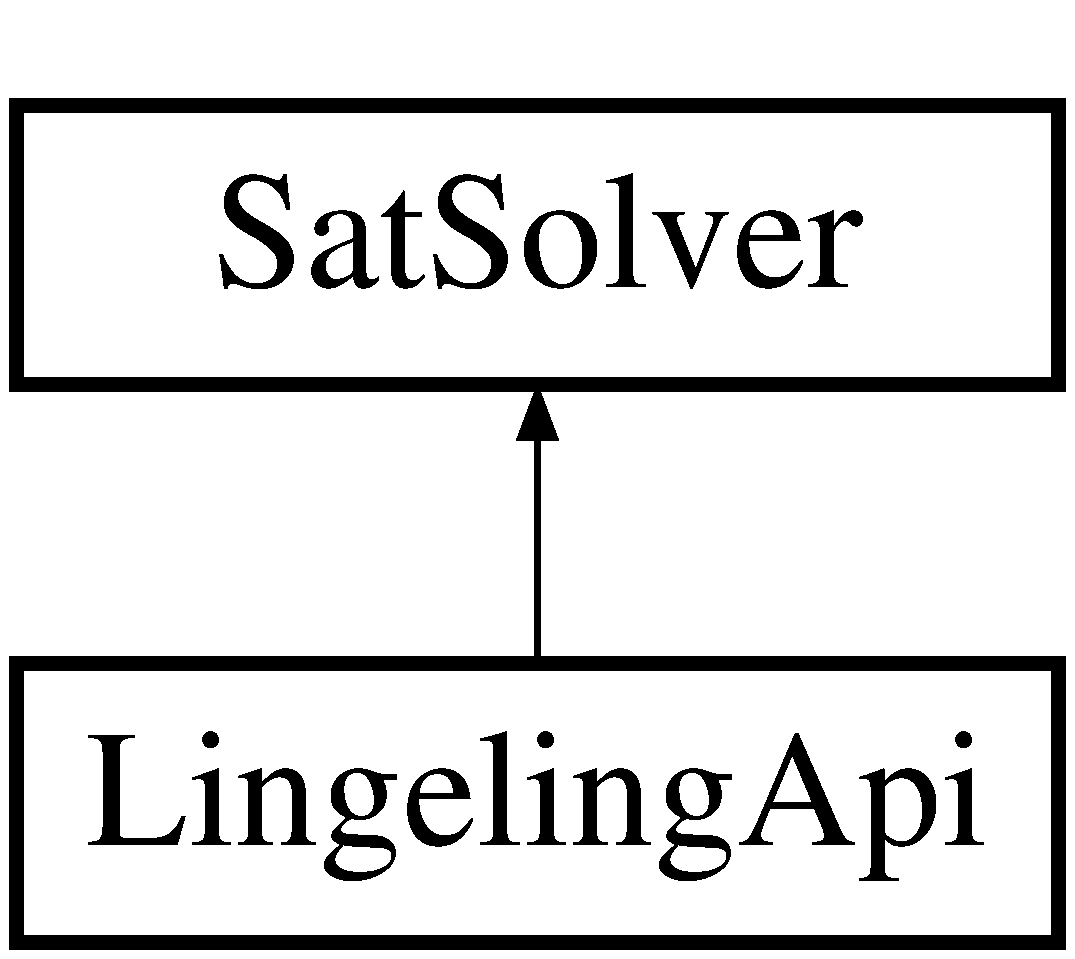
\includegraphics[height=2.000000cm]{classLingelingApi}
\end{center}
\end{figure}
\subsection*{Public Member Functions}
\begin{DoxyCompactItemize}
\item 
\hyperlink{classLingelingApi_a9a66bc58b8bbe631c82d3c80173c947f}{Lingeling\-Api} (bool rand\-\_\-models=false, bool min\-\_\-cores=true)
\begin{DoxyCompactList}\small\item\em Constructor. \end{DoxyCompactList}\item 
virtual \hyperlink{classLingelingApi_aae29bce532ab33b867d5cc4c96f80cd2}{$\sim$\-Lingeling\-Api} ()
\begin{DoxyCompactList}\small\item\em Destructor. \end{DoxyCompactList}\item 
virtual bool \hyperlink{classLingelingApi_a38358f64ded244e2e3d843d0565f0177}{is\-Sat} (const \hyperlink{classCNF}{C\-N\-F} \&cnf)
\begin{DoxyCompactList}\small\item\em Checks if a \hyperlink{classCNF}{C\-N\-F} is satisfiable. \end{DoxyCompactList}\item 
virtual bool \hyperlink{classLingelingApi_a8f147b59f0ebabc35a20d295f28d499f}{is\-Sat\-Model\-Or\-Core} (const \hyperlink{classCNF}{C\-N\-F} \&cnf, const vector$<$ int $>$ \&assumptions, const vector$<$ int $>$ \&vars\-\_\-of\-\_\-interest, vector$<$ int $>$ \&model\-\_\-or\-\_\-core)
\begin{DoxyCompactList}\small\item\em Checks if a \hyperlink{classCNF}{C\-N\-F} is satisfiable and extracts a model or an unsatisfiable core. \end{DoxyCompactList}\item 
virtual void \hyperlink{classLingelingApi_a844da6cbdf38b7cc8abd0b1710350be2}{start\-Incremental\-Session} (const vector$<$ int $>$ \&vars\-\_\-to\-\_\-keep, bool use\-\_\-push=true)
\begin{DoxyCompactList}\small\item\em Starts a new incremental session. \end{DoxyCompactList}\item 
virtual void \hyperlink{classLingelingApi_a4200b2ca7b1694898434ae9764f5baf6}{clear\-Incremental\-Session} ()
\begin{DoxyCompactList}\small\item\em Deletes the solver instance that is used in the incremental session. \end{DoxyCompactList}\item 
virtual void \hyperlink{classLingelingApi_ae9e54e64007c98add90e142a5c38d4bc}{inc\-Add\-C\-N\-F} (const \hyperlink{classCNF}{C\-N\-F} \&cnf)
\begin{DoxyCompactList}\small\item\em Adds a new \hyperlink{classCNF}{C\-N\-F} to the current incremental session. \end{DoxyCompactList}\item 
virtual void \hyperlink{classLingelingApi_afb3e0d0ab541b89ef6c281145f53105f}{inc\-Add\-Clause} (const vector$<$ int $>$ \&clause)
\begin{DoxyCompactList}\small\item\em Adds a new clause to the current incremental session. \end{DoxyCompactList}\item 
virtual void \hyperlink{classLingelingApi_aa5c928ad16d2dc79d42b977237d377e0}{inc\-Add\-Unit\-Clause} (int lit)
\begin{DoxyCompactList}\small\item\em Adds a new unit clause to the current incremental session. \end{DoxyCompactList}\item 
virtual void \hyperlink{classLingelingApi_a54bf3198e6bb2dd3ebda768272337955}{inc\-Add2\-Lit\-Clause} (int lit1, int lit2)
\begin{DoxyCompactList}\small\item\em Adds a new clause consisting of 2 literals to the current incremental session. \end{DoxyCompactList}\item 
virtual void \hyperlink{classLingelingApi_ad05f795bbf472fe5386164a74a8ecd86}{inc\-Add3\-Lit\-Clause} (int lit1, int lit2, int lit3)
\begin{DoxyCompactList}\small\item\em Adds a new clause consisting of 3 literals to the current incremental session. \end{DoxyCompactList}\item 
virtual void \hyperlink{classLingelingApi_a6dc0eb0582d6afda381fc05a5820433c}{inc\-Add\-Cube} (const vector$<$ int $>$ \&cube)
\begin{DoxyCompactList}\small\item\em Adds a new cube to the current incremental session. \end{DoxyCompactList}\item 
virtual void \hyperlink{classLingelingApi_afefd24f97e49aed7cbaf25140a6b7741}{inc\-Add\-Neg\-Cube\-As\-Clause} (const vector$<$ int $>$ \&cube)
\begin{DoxyCompactList}\small\item\em Adds the negation of a given cube (which is a clause) to the incremental session. \end{DoxyCompactList}\item 
virtual bool \hyperlink{classLingelingApi_a7a96e3b1078e40305f8b5e329f0a1e26}{inc\-Is\-Sat} ()
\begin{DoxyCompactList}\small\item\em Checks if a the \hyperlink{classCNF}{C\-N\-F} in the incremental session is satisfiable. \end{DoxyCompactList}\item 
virtual bool \hyperlink{classLingelingApi_a192ddd0f1d27617570c759b3496ea90d}{inc\-Is\-Sat} (const vector$<$ int $>$ \&assumptions)
\begin{DoxyCompactList}\small\item\em Checks if a the \hyperlink{classCNF}{C\-N\-F} in the incremental session is satisfiable under assumptions. \end{DoxyCompactList}\item 
virtual bool \hyperlink{classLingelingApi_a5f70806ab80cb622f4f7286f66284c4e}{inc\-Is\-Sat\-Model\-Or\-Core} (const vector$<$ int $>$ \&assumptions, const vector$<$ int $>$ \&vars\-\_\-of\-\_\-interest, vector$<$ int $>$ \&model\-\_\-or\-\_\-core)
\begin{DoxyCompactList}\small\item\em Checks the \hyperlink{classCNF}{C\-N\-F} in the incremental session and computes a model or unsat core. \end{DoxyCompactList}\item 
virtual bool \hyperlink{classLingelingApi_a95680a60e64dccddbe007ef7d4c8a960}{inc\-Is\-Sat\-Model\-Or\-Core} (const vector$<$ int $>$ \&core\-\_\-assumptions, const vector$<$ int $>$ \&more\-\_\-assumptions, const vector$<$ int $>$ \&vars\-\_\-of\-\_\-interest, vector$<$ int $>$ \&model\-\_\-or\-\_\-core)
\begin{DoxyCompactList}\small\item\em Computes a satisfying assignment or core using additional assumptions. \end{DoxyCompactList}\item 
virtual void \hyperlink{classLingelingApi_a91c858d2a36a4fbe580909a793802a76}{inc\-Push} ()
\begin{DoxyCompactList}\small\item\em Stores the current state of the incremental session on a stack. \end{DoxyCompactList}\item 
virtual void \hyperlink{classLingelingApi_afe43e1243338a332803fff470eedbf7a}{inc\-Pop} ()
\begin{DoxyCompactList}\small\item\em Restores the incremental session back to the point where \hyperlink{classLingelingApi_a91c858d2a36a4fbe580909a793802a76}{inc\-Push()} was called. \end{DoxyCompactList}\item 
void \hyperlink{classSatSolver_a159fc9658709e5aeba2844a09454b2cb}{do\-Min\-Cores} (bool min\-\_\-cores=true)
\begin{DoxyCompactList}\small\item\em Enables or disables the computation of M\-I\-N\-I\-M\-A\-L unsatisfiable cores. \end{DoxyCompactList}\item 
void \hyperlink{classSatSolver_ae229c5e277350710412fce0e867dc566}{do\-Rand\-Models} (bool rand\-\_\-models=true)
\begin{DoxyCompactList}\small\item\em Enables or disables the randomization of satisfying assignments. \end{DoxyCompactList}\end{DoxyCompactItemize}
\subsection*{Protected Types}
\begin{DoxyCompactItemize}
\item 
typedef list$<$ L\-G\-L $\ast$ $>$\\*
\-::const\-\_\-iterator \hyperlink{classLingelingApi_a5c16b047da9b5bd344f30a855dac52e7}{Stack\-Const\-Iter}
\begin{DoxyCompactList}\small\item\em A type for a const-\/iterator over the incremental session stack. \end{DoxyCompactList}\item 
typedef list$<$ L\-G\-L $\ast$ $>$\-::iterator \hyperlink{classLingelingApi_aa4ab290e2a0f65677b6e58b675741535}{Stack\-Iter}
\begin{DoxyCompactList}\small\item\em A type for an iterator over the incremental session stack. \end{DoxyCompactList}\end{DoxyCompactItemize}
\subsection*{Protected Member Functions}
\begin{DoxyCompactItemize}
\item 
void \hyperlink{classLingelingApi_a1b2cec409be65f2bf885593c83d73883}{rand\-Model} (L\-G\-L $\ast$solver, const vector$<$ int $>$ \&assumptions, vector$<$ int $>$ \&model)
\begin{DoxyCompactList}\small\item\em A helper to randomize a satisfying assignment after it has been computed. \end{DoxyCompactList}\end{DoxyCompactItemize}
\subsection*{Protected Attributes}
\begin{DoxyCompactItemize}
\item 
list$<$ L\-G\-L $\ast$ $>$ \hyperlink{classLingelingApi_af9b5703f6611337668def5aaf6be465a}{incr\-\_\-stack\-\_\-}
\begin{DoxyCompactList}\small\item\em A stack of incremental session contexts. \end{DoxyCompactList}\item 
bool \hyperlink{classSatSolver_adfeecebfd09606c82b5c57cfe5aad813}{min\-\_\-cores\-\_\-}
\begin{DoxyCompactList}\small\item\em Indicates if the unsat cores returned by the solver should be minimized further. \end{DoxyCompactList}\item 
bool \hyperlink{classSatSolver_a73fed24d8fb4da85ef82dc53ac5f28c7}{rand\-\_\-models\-\_\-}
\begin{DoxyCompactList}\small\item\em Indicates if satisfying assignments should be randomized. \end{DoxyCompactList}\end{DoxyCompactItemize}
\subsection*{Private Member Functions}
\begin{DoxyCompactItemize}
\item 
\hyperlink{classLingelingApi_ac2716f603b9029e3083a1039eb1ed0bd}{Lingeling\-Api} (const \hyperlink{classLingelingApi}{Lingeling\-Api} \&other)
\begin{DoxyCompactList}\small\item\em Copy constructor. \end{DoxyCompactList}\item 
\hyperlink{classLingelingApi}{Lingeling\-Api} \& \hyperlink{classLingelingApi_a1963aa6729bd9203863010b9bbdb1683}{operator=} (const \hyperlink{classLingelingApi}{Lingeling\-Api} \&other)
\begin{DoxyCompactList}\small\item\em Assignment operator. \end{DoxyCompactList}\end{DoxyCompactItemize}


\subsection{Detailed Description}
Interfaces the Lingeling S\-A\-T-\/solver via its A\-P\-I. 

This class represents an interface to the S\-A\-T-\/solver Lingeling (see \href{http://fmv.jku.at/lingeling/}{\tt http\-://fmv.\-jku.\-at/lingeling/}). It is a concrete implementation of the \hyperlink{classSatSolver}{Sat\-Solver} interface. For a given \hyperlink{classCNF}{C\-N\-F}, this class is able to determine satisfiability. Furthermore, in case of satisfiability, it can extract satisfying assignments. In case of unsatisfiability, it can compute an unsatisfiable core. It can be used in two different ways. In the incremental usage scenario, all information the solver has learned so far is retained. Methods for incremental solving start with 'inc'. Other methods (like \hyperlink{classLingelingApi_a38358f64ded244e2e3d843d0565f0177}{is\-Sat()} or \hyperlink{classLingelingApi_a8f147b59f0ebabc35a20d295f28d499f}{is\-Sat\-Model\-Or\-Core()}) instantiate a fresh solver instance for every call.

\begin{DoxyAuthor}{Author}
Robert Koenighofer (\href{mailto:robert.koenighofer@iaik.tugraz.at}{\tt robert.\-koenighofer@iaik.\-tugraz.\-at}) 
\end{DoxyAuthor}
\begin{DoxyVersion}{Version}
1.\-1.\-0 
\end{DoxyVersion}


Definition at line 55 of file Lingeling\-Api.\-h.



\subsection{Member Typedef Documentation}
\hypertarget{classLingelingApi_a5c16b047da9b5bd344f30a855dac52e7}{\index{Lingeling\-Api@{Lingeling\-Api}!Stack\-Const\-Iter@{Stack\-Const\-Iter}}
\index{Stack\-Const\-Iter@{Stack\-Const\-Iter}!LingelingApi@{Lingeling\-Api}}
\subsubsection[{Stack\-Const\-Iter}]{\setlength{\rightskip}{0pt plus 5cm}list$<$ L\-G\-L $\ast$ $>$\-::const\-\_\-iterator {\bf Lingeling\-Api\-::\-Stack\-Const\-Iter}\hspace{0.3cm}{\ttfamily [protected]}}}\label{classLingelingApi_a5c16b047da9b5bd344f30a855dac52e7}


A type for a const-\/iterator over the incremental session stack. 



Definition at line 390 of file Lingeling\-Api.\-h.

\hypertarget{classLingelingApi_aa4ab290e2a0f65677b6e58b675741535}{\index{Lingeling\-Api@{Lingeling\-Api}!Stack\-Iter@{Stack\-Iter}}
\index{Stack\-Iter@{Stack\-Iter}!LingelingApi@{Lingeling\-Api}}
\subsubsection[{Stack\-Iter}]{\setlength{\rightskip}{0pt plus 5cm}list$<$ L\-G\-L $\ast$ $>$\-::iterator {\bf Lingeling\-Api\-::\-Stack\-Iter}\hspace{0.3cm}{\ttfamily [protected]}}}\label{classLingelingApi_aa4ab290e2a0f65677b6e58b675741535}


A type for an iterator over the incremental session stack. 



Definition at line 396 of file Lingeling\-Api.\-h.



\subsection{Constructor \& Destructor Documentation}
\hypertarget{classLingelingApi_a9a66bc58b8bbe631c82d3c80173c947f}{\index{Lingeling\-Api@{Lingeling\-Api}!Lingeling\-Api@{Lingeling\-Api}}
\index{Lingeling\-Api@{Lingeling\-Api}!LingelingApi@{Lingeling\-Api}}
\subsubsection[{Lingeling\-Api}]{\setlength{\rightskip}{0pt plus 5cm}Lingeling\-Api\-::\-Lingeling\-Api (
\begin{DoxyParamCaption}
\item[{bool}]{rand\-\_\-models = {\ttfamily false}, }
\item[{bool}]{min\-\_\-cores = {\ttfamily true}}
\end{DoxyParamCaption}
)}}\label{classLingelingApi_a9a66bc58b8bbe631c82d3c80173c947f}


Constructor. 


\begin{DoxyParams}{Parameters}
{\em rand\-\_\-models} & A flag indicating if satisfying assignments should be randomized. This is done in a post-\/processing step (values are flipped randomly and then we check if this still constitutes a satisfying assignment). This is expensive. If this parameter is skipped, then satisfying assignments are not randomized. \\
\hline
{\em min\-\_\-cores} & A flag indicating if unsatisfiable cores returned by the solver should be minimized further by trying to drop one literal after the other. This makes the calls slower but produces potentially smaller cubes. \\
\hline
\end{DoxyParams}


Definition at line 38 of file Lingeling\-Api.\-cpp.

\hypertarget{classLingelingApi_aae29bce532ab33b867d5cc4c96f80cd2}{\index{Lingeling\-Api@{Lingeling\-Api}!$\sim$\-Lingeling\-Api@{$\sim$\-Lingeling\-Api}}
\index{$\sim$\-Lingeling\-Api@{$\sim$\-Lingeling\-Api}!LingelingApi@{Lingeling\-Api}}
\subsubsection[{$\sim$\-Lingeling\-Api}]{\setlength{\rightskip}{0pt plus 5cm}Lingeling\-Api\-::$\sim$\-Lingeling\-Api (
\begin{DoxyParamCaption}
{}
\end{DoxyParamCaption}
)\hspace{0.3cm}{\ttfamily [virtual]}}}\label{classLingelingApi_aae29bce532ab33b867d5cc4c96f80cd2}


Destructor. 



Definition at line 45 of file Lingeling\-Api.\-cpp.



References clear\-Incremental\-Session().

\hypertarget{classLingelingApi_ac2716f603b9029e3083a1039eb1ed0bd}{\index{Lingeling\-Api@{Lingeling\-Api}!Lingeling\-Api@{Lingeling\-Api}}
\index{Lingeling\-Api@{Lingeling\-Api}!LingelingApi@{Lingeling\-Api}}
\subsubsection[{Lingeling\-Api}]{\setlength{\rightskip}{0pt plus 5cm}Lingeling\-Api\-::\-Lingeling\-Api (
\begin{DoxyParamCaption}
\item[{const {\bf Lingeling\-Api} \&}]{other}
\end{DoxyParamCaption}
)\hspace{0.3cm}{\ttfamily [private]}}}\label{classLingelingApi_ac2716f603b9029e3083a1039eb1ed0bd}


Copy constructor. 

The copy constructor is disabled (set private) and not implemented.


\begin{DoxyParams}{Parameters}
{\em other} & The source for creating the copy. \\
\hline
\end{DoxyParams}


\subsection{Member Function Documentation}
\hypertarget{classLingelingApi_a4200b2ca7b1694898434ae9764f5baf6}{\index{Lingeling\-Api@{Lingeling\-Api}!clear\-Incremental\-Session@{clear\-Incremental\-Session}}
\index{clear\-Incremental\-Session@{clear\-Incremental\-Session}!LingelingApi@{Lingeling\-Api}}
\subsubsection[{clear\-Incremental\-Session}]{\setlength{\rightskip}{0pt plus 5cm}void Lingeling\-Api\-::clear\-Incremental\-Session (
\begin{DoxyParamCaption}
{}
\end{DoxyParamCaption}
)\hspace{0.3cm}{\ttfamily [virtual]}}}\label{classLingelingApi_a4200b2ca7b1694898434ae9764f5baf6}


Deletes the solver instance that is used in the incremental session. 



Implements \hyperlink{classSatSolver_a8118d2900f7acf31497cd2a27ad3b713}{Sat\-Solver}.



Definition at line 151 of file Lingeling\-Api.\-cpp.



References incr\-\_\-stack\-\_\-.



Referenced by start\-Incremental\-Session(), and $\sim$\-Lingeling\-Api().

\hypertarget{classSatSolver_a159fc9658709e5aeba2844a09454b2cb}{\index{Lingeling\-Api@{Lingeling\-Api}!do\-Min\-Cores@{do\-Min\-Cores}}
\index{do\-Min\-Cores@{do\-Min\-Cores}!LingelingApi@{Lingeling\-Api}}
\subsubsection[{do\-Min\-Cores}]{\setlength{\rightskip}{0pt plus 5cm}void Sat\-Solver\-::do\-Min\-Cores (
\begin{DoxyParamCaption}
\item[{bool}]{min\-\_\-cores = {\ttfamily true}}
\end{DoxyParamCaption}
)\hspace{0.3cm}{\ttfamily [inherited]}}}\label{classSatSolver_a159fc9658709e5aeba2844a09454b2cb}


Enables or disables the computation of M\-I\-N\-I\-M\-A\-L unsatisfiable cores. 


\begin{DoxyParams}{Parameters}
{\em min\-\_\-cores} & A flag indicating if unsatisfiable cores returned by the solver should be minimized further by trying to drop one literal after the other. This makes the calls slower but produces potentially smaller cubes. If the parameter is skipped the computation of minimal cores is enabled. \\
\hline
\end{DoxyParams}


Definition at line 47 of file Sat\-Solver.\-cpp.



References Sat\-Solver\-::min\-\_\-cores\-\_\-.



Referenced by Learn\-Synth\-S\-A\-T\-::compute\-Winning\-Region\-Plain(), Learn\-Synth\-S\-A\-T\-::compute\-Winning\-Region\-Plain\-Dep(), Learn\-Synth\-S\-A\-T\-::compute\-Winning\-Region\-Plain\-Dep2(), Learn\-Synth\-S\-A\-T\-::compute\-Winning\-Region\-R\-G(), Learn\-Synth\-S\-A\-T\-::compute\-Winning\-Region\-R\-G\-R\-C(), Learning\-Impl\-Extractor\-::run\-Learning\-Jiang\-S\-A\-T(), Learning\-Impl\-Extractor\-::run\-Learning\-Jiang\-S\-A\-T\-Inc1(), Learning\-Impl\-Extractor\-::run\-Learning\-Jiang\-S\-A\-T\-Inc2(), Learning\-Impl\-Extractor\-::run\-Learning\-Jiang\-S\-A\-T\-Tmp(), Learning\-Impl\-Extractor\-::run\-Learning\-Jiang\-S\-A\-T\-Tmp\-Ctrl(), and Learning\-Impl\-Extractor\-::run\-Learning\-Jiang\-S\-A\-T\-Tmp\-Ctrl\-Inc2().

\hypertarget{classSatSolver_ae229c5e277350710412fce0e867dc566}{\index{Lingeling\-Api@{Lingeling\-Api}!do\-Rand\-Models@{do\-Rand\-Models}}
\index{do\-Rand\-Models@{do\-Rand\-Models}!LingelingApi@{Lingeling\-Api}}
\subsubsection[{do\-Rand\-Models}]{\setlength{\rightskip}{0pt plus 5cm}void Sat\-Solver\-::do\-Rand\-Models (
\begin{DoxyParamCaption}
\item[{bool}]{rand\-\_\-models = {\ttfamily true}}
\end{DoxyParamCaption}
)\hspace{0.3cm}{\ttfamily [inherited]}}}\label{classSatSolver_ae229c5e277350710412fce0e867dc566}


Enables or disables the randomization of satisfying assignments. 


\begin{DoxyParams}{Parameters}
{\em rand\-\_\-models} & A flag indicating if satisfying assignments should be randomized. This is done in a post-\/processing step (values are flipped randomly and then we check if this still constitutes a satisfying assignment). This is expensive. If this parameter is skipped, then randomization is enabled. \\
\hline
\end{DoxyParams}


Definition at line 53 of file Sat\-Solver.\-cpp.



References Sat\-Solver\-::rand\-\_\-models\-\_\-.



Referenced by Learn\-Synth\-S\-A\-T\-::compute\-Winning\-Region\-Plain(), Learn\-Synth\-S\-A\-T\-::compute\-Winning\-Region\-Plain\-Dep(), Learn\-Synth\-S\-A\-T\-::compute\-Winning\-Region\-Plain\-Dep2(), Learn\-Synth\-S\-A\-T\-::compute\-Winning\-Region\-R\-G(), and Learn\-Synth\-S\-A\-T\-::compute\-Winning\-Region\-R\-G\-R\-C().

\hypertarget{classLingelingApi_a54bf3198e6bb2dd3ebda768272337955}{\index{Lingeling\-Api@{Lingeling\-Api}!inc\-Add2\-Lit\-Clause@{inc\-Add2\-Lit\-Clause}}
\index{inc\-Add2\-Lit\-Clause@{inc\-Add2\-Lit\-Clause}!LingelingApi@{Lingeling\-Api}}
\subsubsection[{inc\-Add2\-Lit\-Clause}]{\setlength{\rightskip}{0pt plus 5cm}void Lingeling\-Api\-::inc\-Add2\-Lit\-Clause (
\begin{DoxyParamCaption}
\item[{int}]{lit1, }
\item[{int}]{lit2}
\end{DoxyParamCaption}
)\hspace{0.3cm}{\ttfamily [virtual]}}}\label{classLingelingApi_a54bf3198e6bb2dd3ebda768272337955}


Adds a new clause consisting of 2 literals to the current incremental session. 

\begin{DoxyPrecond}{Precondition}
\hyperlink{classLingelingApi_a844da6cbdf38b7cc8abd0b1710350be2}{start\-Incremental\-Session()} must have been called before. 
\end{DoxyPrecond}

\begin{DoxyParams}{Parameters}
{\em lit1} & The first literal of the clause to add to the currently open incremental session. If this method is called after solving for the first time, be sure that the passed literal talks about a variables that have been mentioned in vars\-\_\-to\-\_\-keep when calling \hyperlink{classLingelingApi_a844da6cbdf38b7cc8abd0b1710350be2}{start\-Incremental\-Session()}. Otherwise, strange things can happen. \\
\hline
{\em lit2} & The second literal of the clause to add to the currently open incremental session (must be contained in vars\-\_\-to\-\_\-keep as well). \\
\hline
\end{DoxyParams}


Implements \hyperlink{classSatSolver_a791be541b59ef58a29a1c517fca943e7}{Sat\-Solver}.



Definition at line 192 of file Lingeling\-Api.\-cpp.



References incr\-\_\-stack\-\_\-, and M\-A\-S\-S\-E\-R\-T.

\hypertarget{classLingelingApi_ad05f795bbf472fe5386164a74a8ecd86}{\index{Lingeling\-Api@{Lingeling\-Api}!inc\-Add3\-Lit\-Clause@{inc\-Add3\-Lit\-Clause}}
\index{inc\-Add3\-Lit\-Clause@{inc\-Add3\-Lit\-Clause}!LingelingApi@{Lingeling\-Api}}
\subsubsection[{inc\-Add3\-Lit\-Clause}]{\setlength{\rightskip}{0pt plus 5cm}void Lingeling\-Api\-::inc\-Add3\-Lit\-Clause (
\begin{DoxyParamCaption}
\item[{int}]{lit1, }
\item[{int}]{lit2, }
\item[{int}]{lit3}
\end{DoxyParamCaption}
)\hspace{0.3cm}{\ttfamily [virtual]}}}\label{classLingelingApi_ad05f795bbf472fe5386164a74a8ecd86}


Adds a new clause consisting of 3 literals to the current incremental session. 

\begin{DoxyPrecond}{Precondition}
\hyperlink{classLingelingApi_a844da6cbdf38b7cc8abd0b1710350be2}{start\-Incremental\-Session()} must have been called before. 
\end{DoxyPrecond}

\begin{DoxyParams}{Parameters}
{\em lit1} & The first literal of the clause to add to the currently open incremental session. If this method is called after solving for the first time, be sure that the passed literal talks about a variables that have been mentioned in vars\-\_\-to\-\_\-keep when calling \hyperlink{classLingelingApi_a844da6cbdf38b7cc8abd0b1710350be2}{start\-Incremental\-Session()}. Otherwise, strange things can happen. \\
\hline
{\em lit2} & The second literal of the clause to add to the currently open incremental session (must be contained in vars\-\_\-to\-\_\-keep as well). \\
\hline
{\em lit3} & The third literal of the clause to add to the currently open incremental session (must be contained in vars\-\_\-to\-\_\-keep as well). \\
\hline
\end{DoxyParams}


Implements \hyperlink{classSatSolver_abca288874a1b8ab1a90cb274eb885ace}{Sat\-Solver}.



Definition at line 202 of file Lingeling\-Api.\-cpp.



References incr\-\_\-stack\-\_\-, and M\-A\-S\-S\-E\-R\-T.

\hypertarget{classLingelingApi_afb3e0d0ab541b89ef6c281145f53105f}{\index{Lingeling\-Api@{Lingeling\-Api}!inc\-Add\-Clause@{inc\-Add\-Clause}}
\index{inc\-Add\-Clause@{inc\-Add\-Clause}!LingelingApi@{Lingeling\-Api}}
\subsubsection[{inc\-Add\-Clause}]{\setlength{\rightskip}{0pt plus 5cm}void Lingeling\-Api\-::inc\-Add\-Clause (
\begin{DoxyParamCaption}
\item[{const vector$<$ int $>$ \&}]{clause}
\end{DoxyParamCaption}
)\hspace{0.3cm}{\ttfamily [virtual]}}}\label{classLingelingApi_afb3e0d0ab541b89ef6c281145f53105f}


Adds a new clause to the current incremental session. 

\begin{DoxyPrecond}{Precondition}
\hyperlink{classLingelingApi_a844da6cbdf38b7cc8abd0b1710350be2}{start\-Incremental\-Session()} must have been called before. 
\end{DoxyPrecond}

\begin{DoxyParams}{Parameters}
{\em clause} & The clause (a disjunction of literals) to add (conjunct) to the currently open incremental session. If this method is called after solving for the first time, be sure that the passed clause talks only about variables that have been mentioned in vars\-\_\-to\-\_\-keep when calling \hyperlink{classLingelingApi_a844da6cbdf38b7cc8abd0b1710350be2}{start\-Incremental\-Session()}. Otherwise, strange things can happen. \\
\hline
\end{DoxyParams}


Implements \hyperlink{classSatSolver_a9f91c104238b6e091513e0aa46970840}{Sat\-Solver}.



Definition at line 173 of file Lingeling\-Api.\-cpp.



References incr\-\_\-stack\-\_\-, and M\-A\-S\-S\-E\-R\-T.

\hypertarget{classLingelingApi_ae9e54e64007c98add90e142a5c38d4bc}{\index{Lingeling\-Api@{Lingeling\-Api}!inc\-Add\-C\-N\-F@{inc\-Add\-C\-N\-F}}
\index{inc\-Add\-C\-N\-F@{inc\-Add\-C\-N\-F}!LingelingApi@{Lingeling\-Api}}
\subsubsection[{inc\-Add\-C\-N\-F}]{\setlength{\rightskip}{0pt plus 5cm}void Lingeling\-Api\-::inc\-Add\-C\-N\-F (
\begin{DoxyParamCaption}
\item[{const {\bf C\-N\-F} \&}]{cnf}
\end{DoxyParamCaption}
)\hspace{0.3cm}{\ttfamily [virtual]}}}\label{classLingelingApi_ae9e54e64007c98add90e142a5c38d4bc}


Adds a new \hyperlink{classCNF}{C\-N\-F} to the current incremental session. 

\begin{DoxyPrecond}{Precondition}
\hyperlink{classLingelingApi_a844da6cbdf38b7cc8abd0b1710350be2}{start\-Incremental\-Session()} must have been called before. 
\end{DoxyPrecond}

\begin{DoxyParams}{Parameters}
{\em cnf} & The \hyperlink{classCNF}{C\-N\-F} to add to the currently open incremental session. If this method is called after solving for the first time, be sure that the passed \hyperlink{classCNF}{C\-N\-F} talks only about variables that have been mentioned in vars\-\_\-to\-\_\-keep when calling \hyperlink{classLingelingApi_a844da6cbdf38b7cc8abd0b1710350be2}{start\-Incremental\-Session()}. Otherwise, strange things can happen. \\
\hline
\end{DoxyParams}


Implements \hyperlink{classSatSolver_ab2581b192cb2c39a81a416a9f7416c9e}{Sat\-Solver}.



Definition at line 159 of file Lingeling\-Api.\-cpp.



References C\-N\-F\-::get\-Clauses(), incr\-\_\-stack\-\_\-, and M\-A\-S\-S\-E\-R\-T.

\hypertarget{classLingelingApi_a6dc0eb0582d6afda381fc05a5820433c}{\index{Lingeling\-Api@{Lingeling\-Api}!inc\-Add\-Cube@{inc\-Add\-Cube}}
\index{inc\-Add\-Cube@{inc\-Add\-Cube}!LingelingApi@{Lingeling\-Api}}
\subsubsection[{inc\-Add\-Cube}]{\setlength{\rightskip}{0pt plus 5cm}void Lingeling\-Api\-::inc\-Add\-Cube (
\begin{DoxyParamCaption}
\item[{const vector$<$ int $>$ \&}]{cube}
\end{DoxyParamCaption}
)\hspace{0.3cm}{\ttfamily [virtual]}}}\label{classLingelingApi_a6dc0eb0582d6afda381fc05a5820433c}


Adds a new cube to the current incremental session. 

That is, all literals of the cube are added as unit clauses to the current incremental session. For instance, if the cube \mbox{[}2, -\/4, 8\mbox{]} is passed as argument, then this method adds the three unit clauses \mbox{[}2\mbox{]}, \mbox{[}-\/4\mbox{]}, \mbox{[}8\mbox{]}.

\begin{DoxyPrecond}{Precondition}
\hyperlink{classLingelingApi_a844da6cbdf38b7cc8abd0b1710350be2}{start\-Incremental\-Session()} must have been called before. 
\end{DoxyPrecond}

\begin{DoxyParams}{Parameters}
{\em cube} & The cube (a conjunction of literals) to add (conjunct) to the currently open incremental session. All literals of this cube will be added as unit clauses. If this method is called after solving for the first time, be sure that the passed clause talks only about variables that have been mentioned in vars\-\_\-to\-\_\-keep when calling \hyperlink{classLingelingApi_a844da6cbdf38b7cc8abd0b1710350be2}{start\-Incremental\-Session()}. Otherwise, strange things can happen. \\
\hline
\end{DoxyParams}


Implements \hyperlink{classSatSolver_a1f04f34bb04174489ed18d0b62241004}{Sat\-Solver}.



Definition at line 213 of file Lingeling\-Api.\-cpp.



References incr\-\_\-stack\-\_\-, and M\-A\-S\-S\-E\-R\-T.

\hypertarget{classLingelingApi_afefd24f97e49aed7cbaf25140a6b7741}{\index{Lingeling\-Api@{Lingeling\-Api}!inc\-Add\-Neg\-Cube\-As\-Clause@{inc\-Add\-Neg\-Cube\-As\-Clause}}
\index{inc\-Add\-Neg\-Cube\-As\-Clause@{inc\-Add\-Neg\-Cube\-As\-Clause}!LingelingApi@{Lingeling\-Api}}
\subsubsection[{inc\-Add\-Neg\-Cube\-As\-Clause}]{\setlength{\rightskip}{0pt plus 5cm}void Lingeling\-Api\-::inc\-Add\-Neg\-Cube\-As\-Clause (
\begin{DoxyParamCaption}
\item[{const vector$<$ int $>$ \&}]{cube}
\end{DoxyParamCaption}
)\hspace{0.3cm}{\ttfamily [virtual]}}}\label{classLingelingApi_afefd24f97e49aed7cbaf25140a6b7741}


Adds the negation of a given cube (which is a clause) to the incremental session. 

For instance, if the cube \mbox{[}2, -\/4, 8\mbox{]} is passed as argument, then this method adds the clauses \mbox{[}-\/2, 4, -\/8\mbox{]} to the current incremental session.

\begin{DoxyPrecond}{Precondition}
\hyperlink{classLingelingApi_a844da6cbdf38b7cc8abd0b1710350be2}{start\-Incremental\-Session()} must have been called before. 
\end{DoxyPrecond}

\begin{DoxyParams}{Parameters}
{\em cube} & The cube (a conjunction of literals) to negate and add (conjunct) to the currently open incremental session. If this method is called after solving for the first time, be sure that the passed cube talks only about variables that have been mentioned in vars\-\_\-to\-\_\-keep when calling \hyperlink{classLingelingApi_a844da6cbdf38b7cc8abd0b1710350be2}{start\-Incremental\-Session()}. Otherwise, strange things can happen. \\
\hline
\end{DoxyParams}


Implements \hyperlink{classSatSolver_a6be2c564289a59057c4c6728a3aa9c2b}{Sat\-Solver}.



Definition at line 225 of file Lingeling\-Api.\-cpp.



References incr\-\_\-stack\-\_\-, and M\-A\-S\-S\-E\-R\-T.

\hypertarget{classLingelingApi_aa5c928ad16d2dc79d42b977237d377e0}{\index{Lingeling\-Api@{Lingeling\-Api}!inc\-Add\-Unit\-Clause@{inc\-Add\-Unit\-Clause}}
\index{inc\-Add\-Unit\-Clause@{inc\-Add\-Unit\-Clause}!LingelingApi@{Lingeling\-Api}}
\subsubsection[{inc\-Add\-Unit\-Clause}]{\setlength{\rightskip}{0pt plus 5cm}void Lingeling\-Api\-::inc\-Add\-Unit\-Clause (
\begin{DoxyParamCaption}
\item[{int}]{lit}
\end{DoxyParamCaption}
)\hspace{0.3cm}{\ttfamily [virtual]}}}\label{classLingelingApi_aa5c928ad16d2dc79d42b977237d377e0}


Adds a new unit clause to the current incremental session. 

\begin{DoxyPrecond}{Precondition}
\hyperlink{classLingelingApi_a844da6cbdf38b7cc8abd0b1710350be2}{start\-Incremental\-Session()} must have been called before. 
\end{DoxyPrecond}

\begin{DoxyParams}{Parameters}
{\em lit} & The (one and only) literal of the unit clause to add to the currently open incremental session. If this method is called after solving for the first time, be sure that the passed literal talks about a variables that have been mentioned in vars\-\_\-to\-\_\-keep when calling \hyperlink{classLingelingApi_a844da6cbdf38b7cc8abd0b1710350be2}{start\-Incremental\-Session()}. Otherwise, strange things can happen. \\
\hline
\end{DoxyParams}


Implements \hyperlink{classSatSolver_a5b39c45cd2a1abfe96c681515dfddb77}{Sat\-Solver}.



Definition at line 183 of file Lingeling\-Api.\-cpp.



References incr\-\_\-stack\-\_\-, and M\-A\-S\-S\-E\-R\-T.

\hypertarget{classLingelingApi_a7a96e3b1078e40305f8b5e329f0a1e26}{\index{Lingeling\-Api@{Lingeling\-Api}!inc\-Is\-Sat@{inc\-Is\-Sat}}
\index{inc\-Is\-Sat@{inc\-Is\-Sat}!LingelingApi@{Lingeling\-Api}}
\subsubsection[{inc\-Is\-Sat}]{\setlength{\rightskip}{0pt plus 5cm}bool Lingeling\-Api\-::inc\-Is\-Sat (
\begin{DoxyParamCaption}
{}
\end{DoxyParamCaption}
)\hspace{0.3cm}{\ttfamily [virtual]}}}\label{classLingelingApi_a7a96e3b1078e40305f8b5e329f0a1e26}


Checks if a the \hyperlink{classCNF}{C\-N\-F} in the incremental session is satisfiable. 

\begin{DoxyPrecond}{Precondition}
\hyperlink{classLingelingApi_a844da6cbdf38b7cc8abd0b1710350be2}{start\-Incremental\-Session()} must have been called before. 
\end{DoxyPrecond}
\begin{DoxyReturn}{Returns}
True in case of satisfiability, false otherwise. 
\end{DoxyReturn}


Implements \hyperlink{classSatSolver_ab1aab4b96a36b2003450067a3799ae23}{Sat\-Solver}.



Definition at line 235 of file Lingeling\-Api.\-cpp.



References incr\-\_\-stack\-\_\-, and M\-A\-S\-S\-E\-R\-T.

\hypertarget{classLingelingApi_a192ddd0f1d27617570c759b3496ea90d}{\index{Lingeling\-Api@{Lingeling\-Api}!inc\-Is\-Sat@{inc\-Is\-Sat}}
\index{inc\-Is\-Sat@{inc\-Is\-Sat}!LingelingApi@{Lingeling\-Api}}
\subsubsection[{inc\-Is\-Sat}]{\setlength{\rightskip}{0pt plus 5cm}bool Lingeling\-Api\-::inc\-Is\-Sat (
\begin{DoxyParamCaption}
\item[{const vector$<$ int $>$ \&}]{assumptions}
\end{DoxyParamCaption}
)\hspace{0.3cm}{\ttfamily [virtual]}}}\label{classLingelingApi_a192ddd0f1d27617570c759b3496ea90d}


Checks if a the \hyperlink{classCNF}{C\-N\-F} in the incremental session is satisfiable under assumptions. 

This method checks if the \hyperlink{classCNF}{C\-N\-F} in the incremental session is satisfiable given that all literals passed in the vector 'assumptions' are true. The assumptions are not persistently added to the \hyperlink{classCNF}{C\-N\-F} of the incremental session.

\begin{DoxyPrecond}{Precondition}
\hyperlink{classLingelingApi_a844da6cbdf38b7cc8abd0b1710350be2}{start\-Incremental\-Session()} must have been called before. 
\end{DoxyPrecond}

\begin{DoxyParams}{Parameters}
{\em assumptions} & A vector of literals. This method then checks if the \hyperlink{classCNF}{C\-N\-F} of the incremental session is satisfiable given that all literals passed in this vector are true. The assumptions are not persistently added to the \hyperlink{classCNF}{C\-N\-F}. The assumptions must be a subset of the vars\-\_\-to\-\_\-keep passed to \hyperlink{classLingelingApi_a844da6cbdf38b7cc8abd0b1710350be2}{start\-Incremental\-Session()}. \\
\hline
\end{DoxyParams}
\begin{DoxyReturn}{Returns}
True in case of satisfiability, false otherwise. 
\end{DoxyReturn}


Implements \hyperlink{classSatSolver_a1864787a33621efac7fc75fb6b25f080}{Sat\-Solver}.



Definition at line 248 of file Lingeling\-Api.\-cpp.



References incr\-\_\-stack\-\_\-, and M\-A\-S\-S\-E\-R\-T.

\hypertarget{classLingelingApi_a5f70806ab80cb622f4f7286f66284c4e}{\index{Lingeling\-Api@{Lingeling\-Api}!inc\-Is\-Sat\-Model\-Or\-Core@{inc\-Is\-Sat\-Model\-Or\-Core}}
\index{inc\-Is\-Sat\-Model\-Or\-Core@{inc\-Is\-Sat\-Model\-Or\-Core}!LingelingApi@{Lingeling\-Api}}
\subsubsection[{inc\-Is\-Sat\-Model\-Or\-Core}]{\setlength{\rightskip}{0pt plus 5cm}bool Lingeling\-Api\-::inc\-Is\-Sat\-Model\-Or\-Core (
\begin{DoxyParamCaption}
\item[{const vector$<$ int $>$ \&}]{assumptions, }
\item[{const vector$<$ int $>$ \&}]{vars\-\_\-of\-\_\-interest, }
\item[{vector$<$ int $>$ \&}]{model\-\_\-or\-\_\-core}
\end{DoxyParamCaption}
)\hspace{0.3cm}{\ttfamily [virtual]}}}\label{classLingelingApi_a5f70806ab80cb622f4f7286f66284c4e}


Checks the \hyperlink{classCNF}{C\-N\-F} in the incremental session and computes a model or unsat core. 

This method checks if the \hyperlink{classCNF}{C\-N\-F} of the incremental session is satisfiable given that all literals passed in the vector 'assumptions' is true. If this is the case, then a satisfying assignment will be written into model\-\_\-or\-\_\-core. You can specify which variables you want to have in the satisfying assignment using the vars\-\_\-of\-\_\-interest vector. The reason is that your \hyperlink{classCNF}{C\-N\-F} may contain thousands of temporary variables stemming from some Tseitin encoding, but usually one in only interested in the value of a few variables. In case of unsatisfiability, an unsatisfiable core is stored in model\-\_\-or\-\_\-core. The unsatisfiable core is a subset of the literals passed in 'assumptions' such that the \hyperlink{classCNF}{C\-N\-F} is still unsatisfiable when these literals hold.


\begin{DoxyParams}{Parameters}
{\em assumptions} & A vector of literals. This method then checks if the \hyperlink{classCNF}{C\-N\-F} of the incremental session is satisfiable given that all literals passed in this vector are true. The assumptions are not persistently added to the \hyperlink{classCNF}{C\-N\-F}. The assumptions must be a subset of the vars\-\_\-to\-\_\-keep passed to \hyperlink{classLingelingApi_a844da6cbdf38b7cc8abd0b1710350be2}{start\-Incremental\-Session()}. \\
\hline
{\em vars\-\_\-of\-\_\-interest} & The variables for which you want to have a value in case of satisfiability. vars\-\_\-of\-\_\-interest must be a subset of the vars\-\_\-to\-\_\-keep passed to \hyperlink{classLingelingApi_a844da6cbdf38b7cc8abd0b1710350be2}{start\-Incremental\-Session()}. \\
\hline
{\em model\-\_\-or\-\_\-core} & An empty vector. Depending on the outcome of the call, either a satisfying assignment (a cube over the variables passed in vars\-\_\-of\-\_\-interest) or an unsatisfiable core (a subset of the literals passed in 'assumptions') will be written into this vector. \\
\hline
\end{DoxyParams}
\begin{DoxyReturn}{Returns}
True in case of satisfiability (of the \hyperlink{classCNF}{C\-N\-F} of the incremental session in conjunction conjuncted with all assumptions), false otherwise. 
\end{DoxyReturn}


Implements \hyperlink{classSatSolver_ad387fc06bacf2d48847f779c9db8461a}{Sat\-Solver}.



Definition at line 264 of file Lingeling\-Api.\-cpp.



References incr\-\_\-stack\-\_\-, M\-A\-S\-S\-E\-R\-T, Sat\-Solver\-::min\-\_\-cores\-\_\-, Sat\-Solver\-::rand\-\_\-models\-\_\-, rand\-Model(), and Utils\-::remove().

\hypertarget{classLingelingApi_a95680a60e64dccddbe007ef7d4c8a960}{\index{Lingeling\-Api@{Lingeling\-Api}!inc\-Is\-Sat\-Model\-Or\-Core@{inc\-Is\-Sat\-Model\-Or\-Core}}
\index{inc\-Is\-Sat\-Model\-Or\-Core@{inc\-Is\-Sat\-Model\-Or\-Core}!LingelingApi@{Lingeling\-Api}}
\subsubsection[{inc\-Is\-Sat\-Model\-Or\-Core}]{\setlength{\rightskip}{0pt plus 5cm}bool Lingeling\-Api\-::inc\-Is\-Sat\-Model\-Or\-Core (
\begin{DoxyParamCaption}
\item[{const vector$<$ int $>$ \&}]{core\-\_\-assumptions, }
\item[{const vector$<$ int $>$ \&}]{more\-\_\-assumptions, }
\item[{const vector$<$ int $>$ \&}]{vars\-\_\-of\-\_\-interest, }
\item[{vector$<$ int $>$ \&}]{model\-\_\-or\-\_\-core}
\end{DoxyParamCaption}
)\hspace{0.3cm}{\ttfamily [virtual]}}}\label{classLingelingApi_a95680a60e64dccddbe007ef7d4c8a960}


Computes a satisfying assignment or core using additional assumptions. 

In contrast to the previous method, this one allows to define two sets of assumptions. The core\-\_\-assumptions are used as basis for extracting an unsatisfiable core in case of unsatisfiability. The more\-\_\-assumptions are assumed but not considered for the computation of unsatisfiable cores. This is convenient to avoid calls to \hyperlink{classLingelingApi_a91c858d2a36a4fbe580909a793802a76}{inc\-Push()} and \hyperlink{classLingelingApi_afe43e1243338a332803fff470eedbf7a}{inc\-Pop()} when temporarily working under assumptions that should not be minimized for the unsatisfiable core.


\begin{DoxyParams}{Parameters}
{\em core\-\_\-assumptions} & A vector of literals. This method then checks if the \hyperlink{classCNF}{C\-N\-F} of the incremental session is satisfiable given that all literals passed in this vector and all literals passed in more\-\_\-assumptions are true. However, for computing the the unsatisfiable core, only the core\-\_\-assumptions will be minimized and the more\-\_\-assumptions stay as they are. That is, in case of unsatisfiability, model\-\_\-or\-\_\-core will contain a subset X of the core\-\_\-assumptions such that X \& more\-\_\-assumptions \& incremental\-\_\-cnf is still unsatisfiable. core\-\_\-assumptions must be a subset of the vars\-\_\-to\-\_\-keep passed to \hyperlink{classLingelingApi_a844da6cbdf38b7cc8abd0b1710350be2}{start\-Incremental\-Session()}. \\
\hline
{\em more\-\_\-assumptions} & A vector of assumptions that are assumed, but not minimized when an unsatisfiable core is computed. That is, in case of unsatisfiability, model\-\_\-or\-\_\-core will contain a subset X of the core\-\_\-assumptions such that X \& more\-\_\-assumptions \& incremental\-\_\-cnf is still unsatisfiable. more\-\_\-assumptions must be a subset of the vars\-\_\-to\-\_\-keep passed to \hyperlink{classLingelingApi_a844da6cbdf38b7cc8abd0b1710350be2}{start\-Incremental\-Session()}. \\
\hline
{\em vars\-\_\-of\-\_\-interest} & The variables for which you want to have a value in case of satisfiability. vars\-\_\-of\-\_\-interest must be a subset of the vars\-\_\-to\-\_\-keep passed to \hyperlink{classLingelingApi_a844da6cbdf38b7cc8abd0b1710350be2}{start\-Incremental\-Session()}. \\
\hline
{\em model\-\_\-or\-\_\-core} & An empty vector. Depending on the outcome of the call, either a satisfying assignment (a cube over the variables passed in vars\-\_\-of\-\_\-interest) or an unsatisfiable core (a subset of the literals passed in 'core\-\_\-assumptions') will be written into this vector. \\
\hline
\end{DoxyParams}
\begin{DoxyReturn}{Returns}
True in case of satisfiability (of the \hyperlink{classCNF}{C\-N\-F} of the incremental session in conjunction conjuncted with all assumptions), false otherwise. 
\end{DoxyReturn}


Implements \hyperlink{classSatSolver_a29225bfab1f352cae27c68e9bda4d409}{Sat\-Solver}.



Definition at line 329 of file Lingeling\-Api.\-cpp.



References incr\-\_\-stack\-\_\-, M\-A\-S\-S\-E\-R\-T, Sat\-Solver\-::min\-\_\-cores\-\_\-, Sat\-Solver\-::rand\-\_\-models\-\_\-, rand\-Model(), and Utils\-::remove().

\hypertarget{classLingelingApi_afe43e1243338a332803fff470eedbf7a}{\index{Lingeling\-Api@{Lingeling\-Api}!inc\-Pop@{inc\-Pop}}
\index{inc\-Pop@{inc\-Pop}!LingelingApi@{Lingeling\-Api}}
\subsubsection[{inc\-Pop}]{\setlength{\rightskip}{0pt plus 5cm}void Lingeling\-Api\-::inc\-Pop (
\begin{DoxyParamCaption}
{}
\end{DoxyParamCaption}
)\hspace{0.3cm}{\ttfamily [virtual]}}}\label{classLingelingApi_afe43e1243338a332803fff470eedbf7a}


Restores the incremental session back to the point where \hyperlink{classLingelingApi_a91c858d2a36a4fbe580909a793802a76}{inc\-Push()} was called. 



Implements \hyperlink{classSatSolver_a436aae045eb04141c834df0b55947ee5}{Sat\-Solver}.



Definition at line 423 of file Lingeling\-Api.\-cpp.



References incr\-\_\-stack\-\_\-, and M\-A\-S\-S\-E\-R\-T.

\hypertarget{classLingelingApi_a91c858d2a36a4fbe580909a793802a76}{\index{Lingeling\-Api@{Lingeling\-Api}!inc\-Push@{inc\-Push}}
\index{inc\-Push@{inc\-Push}!LingelingApi@{Lingeling\-Api}}
\subsubsection[{inc\-Push}]{\setlength{\rightskip}{0pt plus 5cm}void Lingeling\-Api\-::inc\-Push (
\begin{DoxyParamCaption}
{}
\end{DoxyParamCaption}
)\hspace{0.3cm}{\ttfamily [virtual]}}}\label{classLingelingApi_a91c858d2a36a4fbe580909a793802a76}


Stores the current state of the incremental session on a stack. 

The state can be restored later by calling \hyperlink{classLingelingApi_afe43e1243338a332803fff470eedbf7a}{inc\-Pop()}. 

Implements \hyperlink{classSatSolver_a4da0dff7082a91429e3311d279605be4}{Sat\-Solver}.



Definition at line 413 of file Lingeling\-Api.\-cpp.



References incr\-\_\-stack\-\_\-, and M\-A\-S\-S\-E\-R\-T.

\hypertarget{classLingelingApi_a38358f64ded244e2e3d843d0565f0177}{\index{Lingeling\-Api@{Lingeling\-Api}!is\-Sat@{is\-Sat}}
\index{is\-Sat@{is\-Sat}!LingelingApi@{Lingeling\-Api}}
\subsubsection[{is\-Sat}]{\setlength{\rightskip}{0pt plus 5cm}bool Lingeling\-Api\-::is\-Sat (
\begin{DoxyParamCaption}
\item[{const {\bf C\-N\-F} \&}]{cnf}
\end{DoxyParamCaption}
)\hspace{0.3cm}{\ttfamily [virtual]}}}\label{classLingelingApi_a38358f64ded244e2e3d843d0565f0177}


Checks if a \hyperlink{classCNF}{C\-N\-F} is satisfiable. 

This method is not incremental. At aver call to this method, a new solver instance is created and deleted afterwards. This method does not interfere with an incremental session that may be open in parallel.


\begin{DoxyParams}{Parameters}
{\em cnf} & The \hyperlink{classCNF}{C\-N\-F} formula for which we want to know if it is satisfiable. \\
\hline
\end{DoxyParams}
\begin{DoxyReturn}{Returns}
True in case of satisfiability, false otherwise. 
\end{DoxyReturn}


Implements \hyperlink{classSatSolver_a82f60f60db464fbe5c66a20ad673a573}{Sat\-Solver}.



Definition at line 51 of file Lingeling\-Api.\-cpp.



References C\-N\-F\-::get\-Clauses(), and M\-A\-S\-S\-E\-R\-T.



Referenced by Learn\-Synth\-S\-A\-T\-::debug\-Check\-Win\-Reg(), Learn\-Synth\-Q\-B\-F\-Ind\-::debug\-Check\-Win\-Reg\-Reach(), and is\-Sat\-Model\-Or\-Core().

\hypertarget{classLingelingApi_a8f147b59f0ebabc35a20d295f28d499f}{\index{Lingeling\-Api@{Lingeling\-Api}!is\-Sat\-Model\-Or\-Core@{is\-Sat\-Model\-Or\-Core}}
\index{is\-Sat\-Model\-Or\-Core@{is\-Sat\-Model\-Or\-Core}!LingelingApi@{Lingeling\-Api}}
\subsubsection[{is\-Sat\-Model\-Or\-Core}]{\setlength{\rightskip}{0pt plus 5cm}bool Lingeling\-Api\-::is\-Sat\-Model\-Or\-Core (
\begin{DoxyParamCaption}
\item[{const {\bf C\-N\-F} \&}]{cnf, }
\item[{const vector$<$ int $>$ \&}]{assumptions, }
\item[{const vector$<$ int $>$ \&}]{vars\-\_\-of\-\_\-interest, }
\item[{vector$<$ int $>$ \&}]{model\-\_\-or\-\_\-core}
\end{DoxyParamCaption}
)\hspace{0.3cm}{\ttfamily [virtual]}}}\label{classLingelingApi_a8f147b59f0ebabc35a20d295f28d499f}


Checks if a \hyperlink{classCNF}{C\-N\-F} is satisfiable and extracts a model or an unsatisfiable core. 

This method is not incremental. At aver call to this method, a new solver instance is created and deleted afterwards. This method does not interfere with an incremental session that may be open in parallel. This method checks if the passed \hyperlink{classCNF}{C\-N\-F} is satisfiable given that all literals passed in the vector 'assumptions' is true. If this is the case, then a satisfying assignment will be written into model\-\_\-or\-\_\-core. You can specify which variables you want to have in the satisfying assignment using the vars\-\_\-of\-\_\-interest vector. The reason is that you \hyperlink{classCNF}{C\-N\-F} may contain thousands of temporary variables stemming from some Tseitin encoding, but usually one in only interested in the value of a few variables. In case of unsatisfiability, an unsatisfiable core is stored in model\-\_\-or\-\_\-core. The unsatisfiable core is a subset of the literals passed in 'assumptions' such that the \hyperlink{classCNF}{C\-N\-F} is still unsatisfiable when these literals hold.


\begin{DoxyParams}{Parameters}
{\em cnf} & The \hyperlink{classCNF}{C\-N\-F} formula for which we want to know if it is satisfiable (in conjunction with the assumptions). \\
\hline
{\em assumptions} & A vector of literals. These literals are conjuncted to the \hyperlink{classCNF}{C\-N\-F} before solving. If you do not have any assumptions but want to decide the satisfiability of the cnf only, then simply leave this vector empty. \\
\hline
{\em vars\-\_\-of\-\_\-interest} & The variables for which you want to have a value in case of satisfiability. \\
\hline
{\em model\-\_\-or\-\_\-core} & An empty vector. Depending on the outcome of the call, either a satisfying assignment (a cube over the variables passed in vars\-\_\-of\-\_\-interest) or an unsatisfiable core (a subset of the literals passed in 'assumptions') will be written into this vector. \\
\hline
\end{DoxyParams}
\begin{DoxyReturn}{Returns}
True in case of satisfiability (of the \hyperlink{classCNF}{C\-N\-F} conjuncted with all assumptions), false otherwise. 
\end{DoxyReturn}


Implements \hyperlink{classSatSolver_ad5cfce08969be5aaf5cd705c12c68818}{Sat\-Solver}.



Definition at line 72 of file Lingeling\-Api.\-cpp.



References C\-N\-F\-::add1\-Lit\-Clause(), C\-N\-F\-::get\-Clauses(), is\-Sat(), M\-A\-S\-S\-E\-R\-T, Sat\-Solver\-::min\-\_\-cores\-\_\-, Sat\-Solver\-::rand\-\_\-models\-\_\-, rand\-Model(), and Utils\-::remove().

\hypertarget{classLingelingApi_a1963aa6729bd9203863010b9bbdb1683}{\index{Lingeling\-Api@{Lingeling\-Api}!operator=@{operator=}}
\index{operator=@{operator=}!LingelingApi@{Lingeling\-Api}}
\subsubsection[{operator=}]{\setlength{\rightskip}{0pt plus 5cm}{\bf Lingeling\-Api}\& Lingeling\-Api\-::operator= (
\begin{DoxyParamCaption}
\item[{const {\bf Lingeling\-Api} \&}]{other}
\end{DoxyParamCaption}
)\hspace{0.3cm}{\ttfamily [private]}}}\label{classLingelingApi_a1963aa6729bd9203863010b9bbdb1683}


Assignment operator. 

The assignment operator is disabled (set private) and not implemented.


\begin{DoxyParams}{Parameters}
{\em other} & The source for creating the copy. \\
\hline
\end{DoxyParams}
\begin{DoxyReturn}{Returns}
The result of the assignment, i.\-e, $\ast$this. 
\end{DoxyReturn}
\hypertarget{classLingelingApi_a1b2cec409be65f2bf885593c83d73883}{\index{Lingeling\-Api@{Lingeling\-Api}!rand\-Model@{rand\-Model}}
\index{rand\-Model@{rand\-Model}!LingelingApi@{Lingeling\-Api}}
\subsubsection[{rand\-Model}]{\setlength{\rightskip}{0pt plus 5cm}void Lingeling\-Api\-::rand\-Model (
\begin{DoxyParamCaption}
\item[{L\-G\-L $\ast$}]{solver, }
\item[{const vector$<$ int $>$ \&}]{assumptions, }
\item[{vector$<$ int $>$ \&}]{model}
\end{DoxyParamCaption}
)\hspace{0.3cm}{\ttfamily [protected]}}}\label{classLingelingApi_a1b2cec409be65f2bf885593c83d73883}


A helper to randomize a satisfying assignment after it has been computed. 

This is done by flipping values of variables randomly and then checking if the modified assignment is still satisfies the formula. This is expensive. However, changing the decision heuristic to a random one seems even more expensive in first experiments.

\begin{DoxyPrecond}{Precondition}
solver != N\-U\-L\-L 
\end{DoxyPrecond}

\begin{DoxyParams}{Parameters}
{\em solver} & The solver containing the \hyperlink{classCNF}{C\-N\-F} for which the satisfying assignment has been computed. \\
\hline
{\em assumptions} & Additional assumptions under which the \hyperlink{classCNF}{C\-N\-F} should be solved. This can be an empty vector if there are no assumptions. \\
\hline
{\em model} & The satisfying assignment that has been found and should now be randomized. It will be modified in place, i.\-e., this vector will contain the randomized model after this method is done. \\
\hline
\end{DoxyParams}


Definition at line 432 of file Lingeling\-Api.\-cpp.



References M\-A\-S\-S\-E\-R\-T.



Referenced by inc\-Is\-Sat\-Model\-Or\-Core(), and is\-Sat\-Model\-Or\-Core().

\hypertarget{classLingelingApi_a844da6cbdf38b7cc8abd0b1710350be2}{\index{Lingeling\-Api@{Lingeling\-Api}!start\-Incremental\-Session@{start\-Incremental\-Session}}
\index{start\-Incremental\-Session@{start\-Incremental\-Session}!LingelingApi@{Lingeling\-Api}}
\subsubsection[{start\-Incremental\-Session}]{\setlength{\rightskip}{0pt plus 5cm}void Lingeling\-Api\-::start\-Incremental\-Session (
\begin{DoxyParamCaption}
\item[{const vector$<$ int $>$ \&}]{vars\-\_\-to\-\_\-keep, }
\item[{bool}]{use\-\_\-push = {\ttfamily true}}
\end{DoxyParamCaption}
)\hspace{0.3cm}{\ttfamily [virtual]}}}\label{classLingelingApi_a844da6cbdf38b7cc8abd0b1710350be2}


Starts a new incremental session. 

Every instance of this class can have at most one open incremental session. If there is an old open incremental session it will be closed before. An incremental session allows you to execute sequences of calls, where the information the solver learned in previous calls is retained and may speedup later calls. You can add new clauses between calls, but you cannot remove clauses.


\begin{DoxyParams}{Parameters}
{\em vars\-\_\-to\-\_\-keep} & A set of variables the solver should not optimize away. Clauses added later in an incremental session can only talk about variables contained in this vector. \\
\hline
{\em use\-\_\-push} & A hint to the solver if you are ever going to use \hyperlink{classLingelingApi_a91c858d2a36a4fbe580909a793802a76}{inc\-Push()} or \hyperlink{classLingelingApi_afe43e1243338a332803fff470eedbf7a}{inc\-Pop()}. In the implementation of this class, this information is completely ignored. Other solver implementations (like \hyperlink{classMiniSatApi}{Mini\-Sat\-Api}) do not support push and and pop natively, so we have to make a workaround. This workaround is expensive and we can safe some computation time if we skip it when we will not need it. \\
\hline
\end{DoxyParams}


Implements \hyperlink{classSatSolver_a74603f84c3f2383a5fc44d5a8093cbea}{Sat\-Solver}.



Definition at line 138 of file Lingeling\-Api.\-cpp.



References clear\-Incremental\-Session(), and incr\-\_\-stack\-\_\-.



\subsection{Member Data Documentation}
\hypertarget{classLingelingApi_af9b5703f6611337668def5aaf6be465a}{\index{Lingeling\-Api@{Lingeling\-Api}!incr\-\_\-stack\-\_\-@{incr\-\_\-stack\-\_\-}}
\index{incr\-\_\-stack\-\_\-@{incr\-\_\-stack\-\_\-}!LingelingApi@{Lingeling\-Api}}
\subsubsection[{incr\-\_\-stack\-\_\-}]{\setlength{\rightskip}{0pt plus 5cm}list$<$L\-G\-L$\ast$$>$ Lingeling\-Api\-::incr\-\_\-stack\-\_\-\hspace{0.3cm}{\ttfamily [protected]}}}\label{classLingelingApi_af9b5703f6611337668def5aaf6be465a}


A stack of incremental session contexts. 

The incremental session is store on a stack to support \hyperlink{classLingelingApi_a91c858d2a36a4fbe580909a793802a76}{inc\-Push()} and \hyperlink{classLingelingApi_afe43e1243338a332803fff470eedbf7a}{inc\-Pop()}. The current session is always at the top of the stack (the end of the list). 

Definition at line 384 of file Lingeling\-Api.\-h.



Referenced by clear\-Incremental\-Session(), inc\-Add2\-Lit\-Clause(), inc\-Add3\-Lit\-Clause(), inc\-Add\-Clause(), inc\-Add\-C\-N\-F(), inc\-Add\-Cube(), inc\-Add\-Neg\-Cube\-As\-Clause(), inc\-Add\-Unit\-Clause(), inc\-Is\-Sat(), inc\-Is\-Sat\-Model\-Or\-Core(), inc\-Pop(), inc\-Push(), and start\-Incremental\-Session().

\hypertarget{classSatSolver_adfeecebfd09606c82b5c57cfe5aad813}{\index{Lingeling\-Api@{Lingeling\-Api}!min\-\_\-cores\-\_\-@{min\-\_\-cores\-\_\-}}
\index{min\-\_\-cores\-\_\-@{min\-\_\-cores\-\_\-}!LingelingApi@{Lingeling\-Api}}
\subsubsection[{min\-\_\-cores\-\_\-}]{\setlength{\rightskip}{0pt plus 5cm}bool Sat\-Solver\-::min\-\_\-cores\-\_\-\hspace{0.3cm}{\ttfamily [protected]}, {\ttfamily [inherited]}}}\label{classSatSolver_adfeecebfd09606c82b5c57cfe5aad813}


Indicates if the unsat cores returned by the solver should be minimized further. 



Definition at line 428 of file Sat\-Solver.\-h.



Referenced by Sat\-Solver\-::do\-Min\-Cores(), inc\-Is\-Sat\-Model\-Or\-Core(), Pico\-Sat\-Api\-::inc\-Is\-Sat\-Model\-Or\-Core(), Mini\-Sat\-Api\-::inc\-Is\-Sat\-Model\-Or\-Core(), is\-Sat\-Model\-Or\-Core(), Pico\-Sat\-Api\-::is\-Sat\-Model\-Or\-Core(), and Mini\-Sat\-Api\-::is\-Sat\-Model\-Or\-Core().

\hypertarget{classSatSolver_a73fed24d8fb4da85ef82dc53ac5f28c7}{\index{Lingeling\-Api@{Lingeling\-Api}!rand\-\_\-models\-\_\-@{rand\-\_\-models\-\_\-}}
\index{rand\-\_\-models\-\_\-@{rand\-\_\-models\-\_\-}!LingelingApi@{Lingeling\-Api}}
\subsubsection[{rand\-\_\-models\-\_\-}]{\setlength{\rightskip}{0pt plus 5cm}bool Sat\-Solver\-::rand\-\_\-models\-\_\-\hspace{0.3cm}{\ttfamily [protected]}, {\ttfamily [inherited]}}}\label{classSatSolver_a73fed24d8fb4da85ef82dc53ac5f28c7}


Indicates if satisfying assignments should be randomized. 



Definition at line 433 of file Sat\-Solver.\-h.



Referenced by Sat\-Solver\-::do\-Rand\-Models(), inc\-Is\-Sat\-Model\-Or\-Core(), Pico\-Sat\-Api\-::inc\-Is\-Sat\-Model\-Or\-Core(), Mini\-Sat\-Api\-::inc\-Is\-Sat\-Model\-Or\-Core(), is\-Sat\-Model\-Or\-Core(), Pico\-Sat\-Api\-::is\-Sat\-Model\-Or\-Core(), and Mini\-Sat\-Api\-::is\-Sat\-Model\-Or\-Core().



The documentation for this class was generated from the following files\-:\begin{DoxyCompactItemize}
\item 
src/\hyperlink{LingelingApi_8h}{Lingeling\-Api.\-h}\item 
src/\hyperlink{LingelingApi_8cpp}{Lingeling\-Api.\-cpp}\end{DoxyCompactItemize}

\hypertarget{classLogger}{\section{Logger Class Reference}
\label{classLogger}\index{Logger@{Logger}}
}


Prints messages of different kind, which can all be enabled and disabled.  




{\ttfamily \#include $<$Logger.\-h$>$}

\subsection*{Public Types}
\begin{DoxyCompactItemize}
\item 
enum \hyperlink{classLogger_ac9e601f90bf326ce2088de52018861dc}{Logtype} \{ \\*
\hyperlink{classLogger_ac9e601f90bf326ce2088de52018861dca482a49db2a0d40e2ae358619edb1633e}{E\-R\-R} = 0, 
\hyperlink{classLogger_ac9e601f90bf326ce2088de52018861dca90d291baa55088591aae64883cfc58bd}{W\-R\-N} = 1, 
\hyperlink{classLogger_ac9e601f90bf326ce2088de52018861dca97ed8522dfcbb2cdf29c7f46e583f42f}{R\-E\-S} = 2, 
\hyperlink{classLogger_ac9e601f90bf326ce2088de52018861dca174739f9b95ebbf75fbb89001f72443b}{I\-N\-F} = 3, 
\\*
\hyperlink{classLogger_ac9e601f90bf326ce2088de52018861dcaecb59ecf12f943da56b6944a3053dc09}{D\-B\-G} = 4, 
\hyperlink{classLogger_ac9e601f90bf326ce2088de52018861dca07be7495a7931bee16f5d94b3671f5de}{L\-O\-G} = 5
 \}
\begin{DoxyCompactList}\small\item\em A type for the kind of message. \end{DoxyCompactList}\end{DoxyCompactItemize}
\subsection*{Public Member Functions}
\begin{DoxyCompactItemize}
\item 
void \hyperlink{classLogger_a9ae40dbcf05113315595e387b2776d2e}{enable} (\hyperlink{classLogger_ac9e601f90bf326ce2088de52018861dc}{Logtype} lt)
\begin{DoxyCompactList}\small\item\em Enables the printing of a certain kind of message. \end{DoxyCompactList}\item 
void \hyperlink{classLogger_af314cd99569d9384d419be84b471941b}{disable} (\hyperlink{classLogger_ac9e601f90bf326ce2088de52018861dc}{Logtype} lt)
\begin{DoxyCompactList}\small\item\em Disables the printing of a certain kind of message. \end{DoxyCompactList}\item 
bool \hyperlink{classLogger_a4dd35dedf6e079909fea430eace0ca88}{is\-Enabled} (\hyperlink{classLogger_ac9e601f90bf326ce2088de52018861dc}{Logtype} lt) const 
\begin{DoxyCompactList}\small\item\em Checks if a certain kind of message is enabled. \end{DoxyCompactList}\item 
ostream \& \hyperlink{classLogger_ac1418f03089428bfb7f3805b7709f2cb}{get\-Ostream} (\hyperlink{classLogger_ac9e601f90bf326ce2088de52018861dc}{Logtype} lt)
\begin{DoxyCompactList}\small\item\em Returns the output stream for a certain kind of message. \end{DoxyCompactList}\end{DoxyCompactItemize}
\subsection*{Static Public Member Functions}
\begin{DoxyCompactItemize}
\item 
static \hyperlink{classLogger}{Logger} \& \hyperlink{classLogger_a4aa4d7c3b98f6e12e7ea8253da5ea0cd}{instance} ()
\begin{DoxyCompactList}\small\item\em Returns the one and only instance of this class. \end{DoxyCompactList}\end{DoxyCompactItemize}
\subsection*{Protected Attributes}
\begin{DoxyCompactItemize}
\item 
vector$<$ ostream $\ast$ $>$ \hyperlink{classLogger_a6e3fde7c57b8e2ba82876ad2972c375b}{streams\-\_\-}
\begin{DoxyCompactList}\small\item\em The output streams to be used for the different kinds of messages. \end{DoxyCompactList}\item 
vector$<$ bool $>$ \hyperlink{classLogger_a615ed59ba1b2d79509bfeddcc8406398}{enabled\-\_\-}
\begin{DoxyCompactList}\small\item\em The flags indicating which kind of message is enabled. \end{DoxyCompactList}\end{DoxyCompactItemize}
\subsection*{Static Protected Attributes}
\begin{DoxyCompactItemize}
\item 
static \hyperlink{classLogger}{Logger} $\ast$ \hyperlink{classLogger_a4f56ea837ef338071364583d6368b7c8}{instance\-\_\-} = N\-U\-L\-L
\begin{DoxyCompactList}\small\item\em The one and only instance of this class. \end{DoxyCompactList}\end{DoxyCompactItemize}
\subsection*{Private Member Functions}
\begin{DoxyCompactItemize}
\item 
\hyperlink{classLogger_abc41bfb031d896170c7675fa96a6b30c}{Logger} ()
\begin{DoxyCompactList}\small\item\em Constructor. \end{DoxyCompactList}\item 
virtual \hyperlink{classLogger_acb668a9e186a25fbaad2e4af6d1ed00a}{$\sim$\-Logger} ()
\begin{DoxyCompactList}\small\item\em Destructor. \end{DoxyCompactList}\item 
\hyperlink{classLogger_a25dabaa7b9631ab7e7988b6b610c6f3a}{Logger} (const \hyperlink{classLogger}{Logger} \&other)
\begin{DoxyCompactList}\small\item\em Copy constructor. \end{DoxyCompactList}\item 
\hyperlink{classLogger}{Logger} \& \hyperlink{classLogger_aa2c434460d394a7600e6806d10df9c8c}{operator=} (const \hyperlink{classLogger}{Logger} \&other)
\begin{DoxyCompactList}\small\item\em Assignment operator. \end{DoxyCompactList}\end{DoxyCompactItemize}


\subsection{Detailed Description}
Prints messages of different kind, which can all be enabled and disabled. 

This utility class is able to print 6 different types of messages\-: E\-R\-R\-O\-Rs, W\-A\-R\-N\-I\-N\-Gs R\-E\-S\-U\-L\-Ts, I\-N\-F\-Os, D\-E\-B\-U\-G messages and L\-O\-G messages. Every kind of message can be enabled and disabled. Do not directly print to stdout or stderr but use this class instead (except for special cases like printing messages before this \hyperlink{classLogger}{Logger} has been initialized).

This class is implemented as a Singleton. That is, you cannot instantiate objects of this class with the constructor. Use the method \hyperlink{classLogger_a4aa4d7c3b98f6e12e7ea8253da5ea0cd}{instance() } to obtain the one and only instance of this class.

\begin{DoxyAuthor}{Author}
Robert Koenighofer (\href{mailto:robert.koenighofer@iaik.tugraz.at}{\tt robert.\-koenighofer@iaik.\-tugraz.\-at}) 
\end{DoxyAuthor}
\begin{DoxyVersion}{Version}
1.\-2.\-0 
\end{DoxyVersion}


Definition at line 52 of file Logger.\-h.



\subsection{Member Enumeration Documentation}
\hypertarget{classLogger_ac9e601f90bf326ce2088de52018861dc}{\index{Logger@{Logger}!Logtype@{Logtype}}
\index{Logtype@{Logtype}!Logger@{Logger}}
\subsubsection[{Logtype}]{\setlength{\rightskip}{0pt plus 5cm}enum {\bf Logger\-::\-Logtype}}}\label{classLogger_ac9e601f90bf326ce2088de52018861dc}


A type for the kind of message. 

\begin{Desc}
\item[Enumerator]\par
\begin{description}
\index{E\-R\-R@{E\-R\-R}!Logger@{Logger}}\index{Logger@{Logger}!E\-R\-R@{E\-R\-R}}\item[{\em 
\hypertarget{classLogger_ac9e601f90bf326ce2088de52018861dca482a49db2a0d40e2ae358619edb1633e}{E\-R\-R}\label{classLogger_ac9e601f90bf326ce2088de52018861dca482a49db2a0d40e2ae358619edb1633e}
}]The value for error messages. Use this kind for messages like 'could not open file'. \index{W\-R\-N@{W\-R\-N}!Logger@{Logger}}\index{Logger@{Logger}!W\-R\-N@{W\-R\-N}}\item[{\em 
\hypertarget{classLogger_ac9e601f90bf326ce2088de52018861dca90d291baa55088591aae64883cfc58bd}{W\-R\-N}\label{classLogger_ac9e601f90bf326ce2088de52018861dca90d291baa55088591aae64883cfc58bd}
}]The value for warnings. Use this kind for messages like 'pending signal'. \index{R\-E\-S@{R\-E\-S}!Logger@{Logger}}\index{Logger@{Logger}!R\-E\-S@{R\-E\-S}}\item[{\em 
\hypertarget{classLogger_ac9e601f90bf326ce2088de52018861dca97ed8522dfcbb2cdf29c7f46e583f42f}{R\-E\-S}\label{classLogger_ac9e601f90bf326ce2088de52018861dca97ed8522dfcbb2cdf29c7f46e583f42f}
}]The value for printing results. Use this kind for messages like 'the spec is realizable'. \index{I\-N\-F@{I\-N\-F}!Logger@{Logger}}\index{Logger@{Logger}!I\-N\-F@{I\-N\-F}}\item[{\em 
\hypertarget{classLogger_ac9e601f90bf326ce2088de52018861dca174739f9b95ebbf75fbb89001f72443b}{I\-N\-F}\label{classLogger_ac9e601f90bf326ce2088de52018861dca174739f9b95ebbf75fbb89001f72443b}
}]The value for printing additional information. Use this kind for messages like 'starting to compute a circuit ...'. \index{D\-B\-G@{D\-B\-G}!Logger@{Logger}}\index{Logger@{Logger}!D\-B\-G@{D\-B\-G}}\item[{\em 
\hypertarget{classLogger_ac9e601f90bf326ce2088de52018861dcaecb59ecf12f943da56b6944a3053dc09}{D\-B\-G}\label{classLogger_ac9e601f90bf326ce2088de52018861dcaecb59ecf12f943da56b6944a3053dc09}
}]The value for printing debug messages. Use this kind for messages like 'the aiger literal 4 corresponds to 12 in \hyperlink{classCNF}{C\-N\-F}'. \index{L\-O\-G@{L\-O\-G}!Logger@{Logger}}\index{Logger@{Logger}!L\-O\-G@{L\-O\-G}}\item[{\em 
\hypertarget{classLogger_ac9e601f90bf326ce2088de52018861dca07be7495a7931bee16f5d94b3671f5de}{L\-O\-G}\label{classLogger_ac9e601f90bf326ce2088de52018861dca07be7495a7931bee16f5d94b3671f5de}
}]The value for printing log messages. This is typically used for performance measures in messages like 'computing the winning region took 16 seconds'. \end{description}
\end{Desc}


Definition at line 70 of file Logger.\-h.



\subsection{Constructor \& Destructor Documentation}
\hypertarget{classLogger_abc41bfb031d896170c7675fa96a6b30c}{\index{Logger@{Logger}!Logger@{Logger}}
\index{Logger@{Logger}!Logger@{Logger}}
\subsubsection[{Logger}]{\setlength{\rightskip}{0pt plus 5cm}Logger\-::\-Logger (
\begin{DoxyParamCaption}
{}
\end{DoxyParamCaption}
)\hspace{0.3cm}{\ttfamily [private]}}}\label{classLogger_abc41bfb031d896170c7675fa96a6b30c}


Constructor. 

The constructor is disabled (set private) as this method is implemented as a Singleton. Use the method \hyperlink{classLogger_a4aa4d7c3b98f6e12e7ea8253da5ea0cd}{instance } to obtain the one and only instance of this class. 

Definition at line 45 of file Logger.\-cpp.



References enabled\-\_\-, and streams\-\_\-.



Referenced by instance().

\hypertarget{classLogger_acb668a9e186a25fbaad2e4af6d1ed00a}{\index{Logger@{Logger}!$\sim$\-Logger@{$\sim$\-Logger}}
\index{$\sim$\-Logger@{$\sim$\-Logger}!Logger@{Logger}}
\subsubsection[{$\sim$\-Logger}]{\setlength{\rightskip}{0pt plus 5cm}Logger\-::$\sim$\-Logger (
\begin{DoxyParamCaption}
{}
\end{DoxyParamCaption}
)\hspace{0.3cm}{\ttfamily [private]}, {\ttfamily [virtual]}}}\label{classLogger_acb668a9e186a25fbaad2e4af6d1ed00a}


Destructor. 

The destructor is disabled (set private) as this method is implemented as a Singleton. One cannot instantiate objects of this class, so there is no need to be able to delete them. 

Definition at line 62 of file Logger.\-cpp.



References streams\-\_\-.

\hypertarget{classLogger_a25dabaa7b9631ab7e7988b6b610c6f3a}{\index{Logger@{Logger}!Logger@{Logger}}
\index{Logger@{Logger}!Logger@{Logger}}
\subsubsection[{Logger}]{\setlength{\rightskip}{0pt plus 5cm}Logger\-::\-Logger (
\begin{DoxyParamCaption}
\item[{const {\bf Logger} \&}]{other}
\end{DoxyParamCaption}
)\hspace{0.3cm}{\ttfamily [private]}}}\label{classLogger_a25dabaa7b9631ab7e7988b6b610c6f3a}


Copy constructor. 

The copy constructor is disabled (set private) and not implemented.


\begin{DoxyParams}{Parameters}
{\em other} & The source for creating the copy. \\
\hline
\end{DoxyParams}


\subsection{Member Function Documentation}
\hypertarget{classLogger_af314cd99569d9384d419be84b471941b}{\index{Logger@{Logger}!disable@{disable}}
\index{disable@{disable}!Logger@{Logger}}
\subsubsection[{disable}]{\setlength{\rightskip}{0pt plus 5cm}void Logger\-::disable (
\begin{DoxyParamCaption}
\item[{{\bf Logtype}}]{lt}
\end{DoxyParamCaption}
)}}\label{classLogger_af314cd99569d9384d419be84b471941b}


Disables the printing of a certain kind of message. 

If a message kind is disabled, all messaged of this type are discarded.


\begin{DoxyParams}{Parameters}
{\em lt} & The kind of message to disable. \\
\hline
\end{DoxyParams}


Definition at line 73 of file Logger.\-cpp.



References enabled\-\_\-.



Referenced by Options\-::init\-Logger().

\hypertarget{classLogger_a9ae40dbcf05113315595e387b2776d2e}{\index{Logger@{Logger}!enable@{enable}}
\index{enable@{enable}!Logger@{Logger}}
\subsubsection[{enable}]{\setlength{\rightskip}{0pt plus 5cm}void Logger\-::enable (
\begin{DoxyParamCaption}
\item[{{\bf Logtype}}]{lt}
\end{DoxyParamCaption}
)}}\label{classLogger_a9ae40dbcf05113315595e387b2776d2e}


Enables the printing of a certain kind of message. 

If a message kind is disabled, all messaged of this type are discarded.


\begin{DoxyParams}{Parameters}
{\em lt} & The kind of message to enable. \\
\hline
\end{DoxyParams}


Definition at line 79 of file Logger.\-cpp.



References enabled\-\_\-.



Referenced by Options\-::init\-Logger().

\hypertarget{classLogger_ac1418f03089428bfb7f3805b7709f2cb}{\index{Logger@{Logger}!get\-Ostream@{get\-Ostream}}
\index{get\-Ostream@{get\-Ostream}!Logger@{Logger}}
\subsubsection[{get\-Ostream}]{\setlength{\rightskip}{0pt plus 5cm}ostream \& Logger\-::get\-Ostream (
\begin{DoxyParamCaption}
\item[{{\bf Logtype}}]{lt}
\end{DoxyParamCaption}
)}}\label{classLogger_ac1418f03089428bfb7f3805b7709f2cb}


Returns the output stream for a certain kind of message. 

Use this method to pipe arbitrary messages into the requested streams. See also the macros 
\begin{DoxyItemize}
\item \hyperlink{Logger_8h_ab46d591f7a5eb63fee458a99279a2d00}{L\-\_\-\-E\-R\-R} 
\item \hyperlink{Logger_8h_aafa8924b4aff539836a162a1cdf5e047}{L\-\_\-\-W\-R\-N} 
\item \hyperlink{Logger_8h_adf55585b6b559a75e33ee291410f9a9e}{L\-\_\-\-R\-E\-S} 
\item \hyperlink{Logger_8h_a5442b95c710d1b2d4c306693fce02997}{L\-\_\-\-I\-N\-F} 
\item \hyperlink{Logger_8h_a5ba9fef95c1aa2be83162fd9f0992c05}{L\-\_\-\-D\-B\-G} 
\item \hyperlink{Logger_8h_a081139c373685d15bfc9f0afebe00542}{L\-\_\-\-L\-O\-G} 
\end{DoxyItemize}which might be more convenient to use.

\begin{DoxyNote}{Note}
This method does not check if the particular kind of message is enabled or disabled, i.\-e, it allows you to print messages although they are disabled. 
\end{DoxyNote}

\begin{DoxyParams}{Parameters}
{\em lt} & The kind of message for which the output stream is requested. \\
\hline
\end{DoxyParams}
\begin{DoxyReturn}{Returns}
The output stream for this message. 
\end{DoxyReturn}


Definition at line 91 of file Logger.\-cpp.



References M\-A\-S\-S\-E\-R\-T, and streams\-\_\-.

\hypertarget{classLogger_a4aa4d7c3b98f6e12e7ea8253da5ea0cd}{\index{Logger@{Logger}!instance@{instance}}
\index{instance@{instance}!Logger@{Logger}}
\subsubsection[{instance}]{\setlength{\rightskip}{0pt plus 5cm}{\bf Logger} \& Logger\-::instance (
\begin{DoxyParamCaption}
{}
\end{DoxyParamCaption}
)\hspace{0.3cm}{\ttfamily [static]}}}\label{classLogger_a4aa4d7c3b98f6e12e7ea8253da5ea0cd}


Returns the one and only instance of this class. 

This class is implemented as a Singleton. That is, you cannot instantiate objects of this class with the constructor. Use this method to obtain the one and only instance of this class.

\begin{DoxyReturn}{Returns}
The one and only instance of this class. 
\end{DoxyReturn}


Definition at line 36 of file Logger.\-cpp.



References instance\-\_\-, Logger(), and M\-A\-S\-S\-E\-R\-T.



Referenced by Learn\-Synth\-Q\-B\-F\-Inc\-::compute\-Winning\-Region\-All(), Learn\-Synth\-Q\-B\-F\-::compute\-Winning\-Region\-All(), Learn\-Synth\-Q\-B\-F\-Ind\-::compute\-Winning\-Region\-All(), Learn\-Synth\-Q\-B\-F\-Inc\-::compute\-Winning\-Region\-All\-Pool(), Learn\-Synth\-Q\-B\-F\-Inc\-::compute\-Winning\-Region\-All\-Push(), Learn\-Synth\-Q\-B\-F\-Inc\-::compute\-Winning\-Region\-One(), Learn\-Synth\-Q\-B\-F\-::compute\-Winning\-Region\-One(), Learn\-Synth\-Q\-B\-F\-Ind\-::compute\-Winning\-Region\-One(), Learn\-Synth\-Q\-B\-F\-Inc\-::compute\-Winning\-Region\-One\-Pool(), Learn\-Synth\-Q\-B\-F\-Inc\-::compute\-Winning\-Region\-One\-Push(), Learn\-Synth\-Q\-B\-F\-::compute\-Winning\-Region\-One\-S\-A\-T(), and Options\-::init\-Logger().

\hypertarget{classLogger_a4dd35dedf6e079909fea430eace0ca88}{\index{Logger@{Logger}!is\-Enabled@{is\-Enabled}}
\index{is\-Enabled@{is\-Enabled}!Logger@{Logger}}
\subsubsection[{is\-Enabled}]{\setlength{\rightskip}{0pt plus 5cm}bool Logger\-::is\-Enabled (
\begin{DoxyParamCaption}
\item[{{\bf Logtype}}]{lt}
\end{DoxyParamCaption}
) const}}\label{classLogger_a4dd35dedf6e079909fea430eace0ca88}


Checks if a certain kind of message is enabled. 

If a message kind is disabled, all messaged of this type are discarded.


\begin{DoxyParams}{Parameters}
{\em lt} & The kind of message in question. \\
\hline
\end{DoxyParams}
\begin{DoxyReturn}{Returns}
True if this kind of message is enabled, false if it is disabled. 
\end{DoxyReturn}


Definition at line 85 of file Logger.\-cpp.



References enabled\-\_\-.



Referenced by Learn\-Synth\-Q\-B\-F\-Inc\-::compute\-Winning\-Region\-All(), Learn\-Synth\-Q\-B\-F\-::compute\-Winning\-Region\-All(), Learn\-Synth\-Q\-B\-F\-Ind\-::compute\-Winning\-Region\-All(), Learn\-Synth\-Q\-B\-F\-Inc\-::compute\-Winning\-Region\-All\-Pool(), Learn\-Synth\-Q\-B\-F\-Inc\-::compute\-Winning\-Region\-All\-Push(), Learn\-Synth\-Q\-B\-F\-Inc\-::compute\-Winning\-Region\-One(), Learn\-Synth\-Q\-B\-F\-::compute\-Winning\-Region\-One(), Learn\-Synth\-Q\-B\-F\-Ind\-::compute\-Winning\-Region\-One(), Learn\-Synth\-Q\-B\-F\-Inc\-::compute\-Winning\-Region\-One\-Pool(), Learn\-Synth\-Q\-B\-F\-Inc\-::compute\-Winning\-Region\-One\-Push(), and Learn\-Synth\-Q\-B\-F\-::compute\-Winning\-Region\-One\-S\-A\-T().

\hypertarget{classLogger_aa2c434460d394a7600e6806d10df9c8c}{\index{Logger@{Logger}!operator=@{operator=}}
\index{operator=@{operator=}!Logger@{Logger}}
\subsubsection[{operator=}]{\setlength{\rightskip}{0pt plus 5cm}{\bf Logger}\& Logger\-::operator= (
\begin{DoxyParamCaption}
\item[{const {\bf Logger} \&}]{other}
\end{DoxyParamCaption}
)\hspace{0.3cm}{\ttfamily [private]}}}\label{classLogger_aa2c434460d394a7600e6806d10df9c8c}


Assignment operator. 

The assignment operator is disabled (set private) and not implemented.


\begin{DoxyParams}{Parameters}
{\em other} & The source for creating the copy. \\
\hline
\end{DoxyParams}
\begin{DoxyReturn}{Returns}
The result of the assignment, i.\-e, $\ast$this. 
\end{DoxyReturn}


\subsection{Member Data Documentation}
\hypertarget{classLogger_a615ed59ba1b2d79509bfeddcc8406398}{\index{Logger@{Logger}!enabled\-\_\-@{enabled\-\_\-}}
\index{enabled\-\_\-@{enabled\-\_\-}!Logger@{Logger}}
\subsubsection[{enabled\-\_\-}]{\setlength{\rightskip}{0pt plus 5cm}vector$<$bool$>$ Logger\-::enabled\-\_\-\hspace{0.3cm}{\ttfamily [protected]}}}\label{classLogger_a615ed59ba1b2d79509bfeddcc8406398}


The flags indicating which kind of message is enabled. 

The order in the array is as following\-: 
\begin{DoxyItemize}
\item enabled\-\_\-\mbox{[}0\mbox{]} is true if errors are enabled. 
\item enabled\-\_\-\mbox{[}1\mbox{]} is true if warnings are enabled. 
\item enabled\-\_\-\mbox{[}2\mbox{]} is true if results are enabled. 
\item enabled\-\_\-\mbox{[}3\mbox{]} is true if infos are enabled. 
\item enabled\-\_\-\mbox{[}4\mbox{]} is true if debug messages are enabled. 
\item enabled\-\_\-\mbox{[}5\mbox{]} is true if log messages are enabled. 
\end{DoxyItemize}

Definition at line 201 of file Logger.\-h.



Referenced by disable(), enable(), is\-Enabled(), and Logger().

\hypertarget{classLogger_a4f56ea837ef338071364583d6368b7c8}{\index{Logger@{Logger}!instance\-\_\-@{instance\-\_\-}}
\index{instance\-\_\-@{instance\-\_\-}!Logger@{Logger}}
\subsubsection[{instance\-\_\-}]{\setlength{\rightskip}{0pt plus 5cm}{\bf Logger} $\ast$ Logger\-::instance\-\_\- = N\-U\-L\-L\hspace{0.3cm}{\ttfamily [static]}, {\ttfamily [protected]}}}\label{classLogger_a4f56ea837ef338071364583d6368b7c8}


The one and only instance of this class. 



Definition at line 171 of file Logger.\-h.



Referenced by instance().

\hypertarget{classLogger_a6e3fde7c57b8e2ba82876ad2972c375b}{\index{Logger@{Logger}!streams\-\_\-@{streams\-\_\-}}
\index{streams\-\_\-@{streams\-\_\-}!Logger@{Logger}}
\subsubsection[{streams\-\_\-}]{\setlength{\rightskip}{0pt plus 5cm}vector$<$ostream$\ast$$>$ Logger\-::streams\-\_\-\hspace{0.3cm}{\ttfamily [protected]}}}\label{classLogger_a6e3fde7c57b8e2ba82876ad2972c375b}


The output streams to be used for the different kinds of messages. 

The order in the array is as following\-: 
\begin{DoxyItemize}
\item streams\-\_\-\mbox{[}0\mbox{]} is the output stream for errors (Logtype\-::\-E\-R\-R) 
\item streams\-\_\-\mbox{[}1\mbox{]} is the output stream for warnings (Logtype\-::\-W\-R\-N) 
\item streams\-\_\-\mbox{[}2\mbox{]} is the output stream for results (Logtype\-::\-R\-E\-S) 
\item streams\-\_\-\mbox{[}3\mbox{]} is the output stream for infos (Logtype\-::\-I\-N\-F) 
\item streams\-\_\-\mbox{[}4\mbox{]} is the output stream for debug messages (Logtype\-::\-D\-B\-G) 
\item streams\-\_\-\mbox{[}5\mbox{]} is the output stream for log messages (Logtype\-::\-L\-O\-G) 
\end{DoxyItemize}

Definition at line 186 of file Logger.\-h.



Referenced by get\-Ostream(), Logger(), and $\sim$\-Logger().



The documentation for this class was generated from the following files\-:\begin{DoxyCompactItemize}
\item 
src/\hyperlink{Logger_8h}{Logger.\-h}\item 
src/\hyperlink{Logger_8cpp}{Logger.\-cpp}\end{DoxyCompactItemize}

\hypertarget{classMiniSatApi}{\section{Mini\-Sat\-Api Class Reference}
\label{classMiniSatApi}\index{Mini\-Sat\-Api@{Mini\-Sat\-Api}}
}


Interfaces the Mini\-Sat S\-A\-T-\/solver via its A\-P\-I.  




{\ttfamily \#include $<$Mini\-Sat\-Api.\-h$>$}

Inheritance diagram for Mini\-Sat\-Api\-:\begin{figure}[H]
\begin{center}
\leavevmode
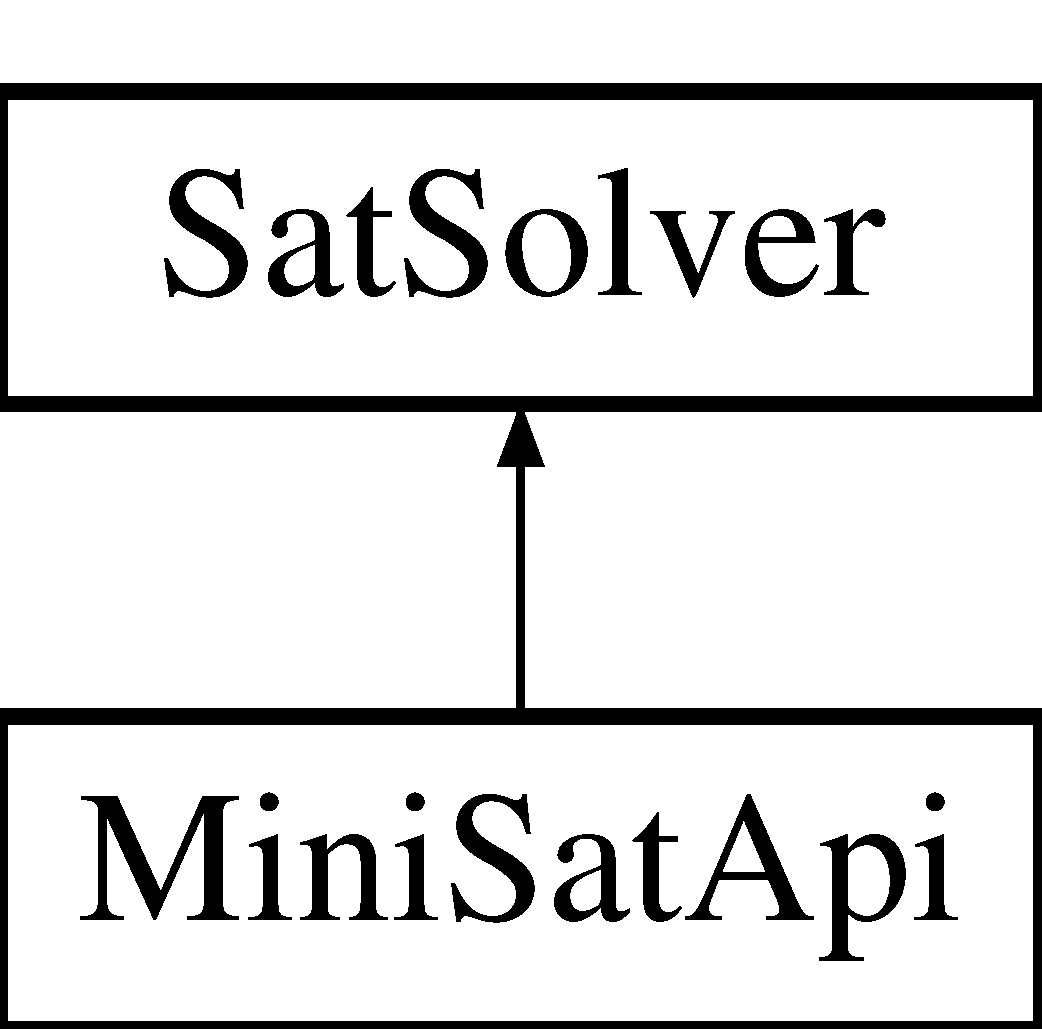
\includegraphics[height=2.000000cm]{classMiniSatApi}
\end{center}
\end{figure}
\subsection*{Public Member Functions}
\begin{DoxyCompactItemize}
\item 
\hyperlink{classMiniSatApi_a1252284d34189f954aaf497b3441b182}{Mini\-Sat\-Api} (bool rand\-\_\-models=false, bool min\-\_\-cores=true)
\begin{DoxyCompactList}\small\item\em Constructor. \end{DoxyCompactList}\item 
virtual \hyperlink{classMiniSatApi_ac45e31c4ce50ddd87df83d97d4c3ac2e}{$\sim$\-Mini\-Sat\-Api} ()
\begin{DoxyCompactList}\small\item\em Destructor. \end{DoxyCompactList}\item 
virtual bool \hyperlink{classMiniSatApi_a73b93ecb947723a96ef6fbd436640e12}{is\-Sat} (const \hyperlink{classCNF}{C\-N\-F} \&cnf)
\begin{DoxyCompactList}\small\item\em Checks if a \hyperlink{classCNF}{C\-N\-F} is satisfiable. \end{DoxyCompactList}\item 
virtual bool \hyperlink{classMiniSatApi_a7f846d8c4a5a652cb83460852c09dfb3}{is\-Sat\-Model\-Or\-Core} (const \hyperlink{classCNF}{C\-N\-F} \&cnf, const vector$<$ int $>$ \&assumptions, const vector$<$ int $>$ \&vars\-\_\-of\-\_\-interest, vector$<$ int $>$ \&model\-\_\-or\-\_\-core)
\begin{DoxyCompactList}\small\item\em Checks if a \hyperlink{classCNF}{C\-N\-F} is satisfiable and extracts a model or an unsatisfiable core. \end{DoxyCompactList}\item 
virtual void \hyperlink{classMiniSatApi_afe6f184e440ffe7f9b3a86045c15b450}{start\-Incremental\-Session} (const vector$<$ int $>$ \&vars\-\_\-to\-\_\-keep, bool use\-\_\-push=true)
\begin{DoxyCompactList}\small\item\em Starts a new incremental session. \end{DoxyCompactList}\item 
virtual void \hyperlink{classMiniSatApi_a237754c78357ed0a84894e811806b618}{clear\-Incremental\-Session} ()
\begin{DoxyCompactList}\small\item\em Deletes the solver instance that is used in the incremental session. \end{DoxyCompactList}\item 
virtual void \hyperlink{classMiniSatApi_ae5ffe2811e01051c5206c9e4865a7102}{inc\-Add\-C\-N\-F} (const \hyperlink{classCNF}{C\-N\-F} \&cnf)
\begin{DoxyCompactList}\small\item\em Adds a new \hyperlink{classCNF}{C\-N\-F} to the current incremental session. \end{DoxyCompactList}\item 
virtual void \hyperlink{classMiniSatApi_af2115a84419b7480ff55b747f7ddd60a}{inc\-Add\-Clause} (const vector$<$ int $>$ \&clause)
\begin{DoxyCompactList}\small\item\em Adds a new clause to the current incremental session. \end{DoxyCompactList}\item 
virtual void \hyperlink{classMiniSatApi_ade09bb38667bb23f2ac993e2d6c66408}{inc\-Add\-Unit\-Clause} (int lit)
\begin{DoxyCompactList}\small\item\em Adds a new unit clause to the current incremental session. \end{DoxyCompactList}\item 
virtual void \hyperlink{classMiniSatApi_a56c4758ee7466cd7fa48a682fee76fd3}{inc\-Add2\-Lit\-Clause} (int lit1, int lit2)
\begin{DoxyCompactList}\small\item\em Adds a new clause consisting of 2 literals to the current incremental session. \end{DoxyCompactList}\item 
virtual void \hyperlink{classMiniSatApi_aee9556c8c5de695fa5d7aa7cfde57877}{inc\-Add3\-Lit\-Clause} (int lit1, int lit2, int lit3)
\begin{DoxyCompactList}\small\item\em Adds a new clause consisting of 3 literals to the current incremental session. \end{DoxyCompactList}\item 
virtual void \hyperlink{classMiniSatApi_a41e16a2e8757846fa17e010c5cc1ff16}{inc\-Add\-Cube} (const vector$<$ int $>$ \&cube)
\begin{DoxyCompactList}\small\item\em Adds a new cube to the current incremental session. \end{DoxyCompactList}\item 
virtual void \hyperlink{classMiniSatApi_a49afe5c41bb036a31f65f98621e82846}{inc\-Add\-Neg\-Cube\-As\-Clause} (const vector$<$ int $>$ \&cube)
\begin{DoxyCompactList}\small\item\em Adds the negation of a given cube (which is a clause) to the incremental session. \end{DoxyCompactList}\item 
virtual bool \hyperlink{classMiniSatApi_a4c6ba65381002eb3f90e8e0df1606759}{inc\-Is\-Sat} ()
\begin{DoxyCompactList}\small\item\em Checks if a the \hyperlink{classCNF}{C\-N\-F} in the incremental session is satisfiable. \end{DoxyCompactList}\item 
virtual bool \hyperlink{classMiniSatApi_a40421bac2739bacb68f3c7083810694b}{inc\-Is\-Sat} (const vector$<$ int $>$ \&assumptions)
\begin{DoxyCompactList}\small\item\em Checks if a the \hyperlink{classCNF}{C\-N\-F} in the incremental session is satisfiable under assumptions. \end{DoxyCompactList}\item 
virtual bool \hyperlink{classMiniSatApi_afb886d40bb45b5cf2fadb7aee1a06b3e}{inc\-Is\-Sat\-Model\-Or\-Core} (const vector$<$ int $>$ \&assumptions, const vector$<$ int $>$ \&vars\-\_\-of\-\_\-interest, vector$<$ int $>$ \&model\-\_\-or\-\_\-core)
\begin{DoxyCompactList}\small\item\em Checks the \hyperlink{classCNF}{C\-N\-F} in the incremental session and computes a model or unsat core. \end{DoxyCompactList}\item 
virtual bool \hyperlink{classMiniSatApi_a776b2b0563b52f52152dcec931b7f557}{inc\-Is\-Sat\-Model\-Or\-Core} (const vector$<$ int $>$ \&core\-\_\-assumptions, const vector$<$ int $>$ \&more\-\_\-assumptions, const vector$<$ int $>$ \&vars\-\_\-of\-\_\-interest, vector$<$ int $>$ \&model\-\_\-or\-\_\-core)
\begin{DoxyCompactList}\small\item\em Computes a satisfying assignment or core using additional assumptions. \end{DoxyCompactList}\item 
virtual void \hyperlink{classMiniSatApi_a27013ace25320f68252bef5ba9f2e9ad}{inc\-Push} ()
\begin{DoxyCompactList}\small\item\em Stores the current state of the incremental session on a stack. \end{DoxyCompactList}\item 
virtual void \hyperlink{classMiniSatApi_af388f97db15f77baeb420a8fef74ca6a}{inc\-Pop} ()
\begin{DoxyCompactList}\small\item\em Restores the incremental session back to the point where \hyperlink{classMiniSatApi_a27013ace25320f68252bef5ba9f2e9ad}{inc\-Push()} was called. \end{DoxyCompactList}\item 
void \hyperlink{classSatSolver_a159fc9658709e5aeba2844a09454b2cb}{do\-Min\-Cores} (bool min\-\_\-cores=true)
\begin{DoxyCompactList}\small\item\em Enables or disables the computation of M\-I\-N\-I\-M\-A\-L unsatisfiable cores. \end{DoxyCompactList}\item 
void \hyperlink{classSatSolver_ae229c5e277350710412fce0e867dc566}{do\-Rand\-Models} (bool rand\-\_\-models=true)
\begin{DoxyCompactList}\small\item\em Enables or disables the randomization of satisfying assignments. \end{DoxyCompactList}\end{DoxyCompactItemize}
\subsection*{Protected Types}
\begin{DoxyCompactItemize}
\item 
typedef list$<$ Minisat\-::\-Solver $\ast$ $>$\\*
\-::const\-\_\-iterator \hyperlink{classMiniSatApi_aa4c233a841e489de9a59622e18df4678}{Stack\-Const\-Iter}
\begin{DoxyCompactList}\small\item\em A type for a const-\/iterator over the incremental session stack. \end{DoxyCompactList}\item 
typedef list$<$ Minisat\-::\-Solver $\ast$ $>$\\*
\-::iterator \hyperlink{classMiniSatApi_a46469116348b199bae1b92d209b969c0}{Stack\-Iter}
\begin{DoxyCompactList}\small\item\em A type for an iterator over the incremental session stack. \end{DoxyCompactList}\item 
typedef list$<$ \hyperlink{classCNF}{C\-N\-F} $\ast$ $>$\\*
\-::const\-\_\-iterator \hyperlink{classMiniSatApi_a1d7b9074d64167fb10552e58a9a84ddb}{Stack\-C\-N\-F\-Const\-Iter}
\begin{DoxyCompactList}\small\item\em A type for a const-\/iterator over the C\-N\-Fs of the incremental sessions. \end{DoxyCompactList}\item 
typedef list$<$ \hyperlink{classCNF}{C\-N\-F} $\ast$ $>$\-::iterator \hyperlink{classMiniSatApi_a12ef23c063731cbdb7405de0e670f6a7}{Stack\-C\-N\-F\-Iter}
\begin{DoxyCompactList}\small\item\em A type for an iterator over the C\-N\-Fs of the incremental sessions. \end{DoxyCompactList}\end{DoxyCompactItemize}
\subsection*{Protected Attributes}
\begin{DoxyCompactItemize}
\item 
list$<$ Minisat\-::\-Solver $\ast$ $>$ \hyperlink{classMiniSatApi_ab9dcac91d11eef23cc40d7478464c414}{incr\-\_\-stack\-\_\-}
\begin{DoxyCompactList}\small\item\em A stack of incremental session contexts. \end{DoxyCompactList}\item 
list$<$ \hyperlink{classCNF}{C\-N\-F} $\ast$ $>$ \hyperlink{classMiniSatApi_aca2da2d02879e4a05c09124ff84cc4cd}{incr\-\_\-stack\-\_\-cnfs\-\_\-}
\begin{DoxyCompactList}\small\item\em A C\-N\-Fs that are stored in the incremental session contexts. \end{DoxyCompactList}\item 
bool \hyperlink{classMiniSatApi_a9d1530348f713264a41d6115e4cfb62e}{use\-\_\-push\-\_\-}
\begin{DoxyCompactList}\small\item\em A flag indicating if \hyperlink{classMiniSatApi_a27013ace25320f68252bef5ba9f2e9ad}{inc\-Push()} and \hyperlink{classMiniSatApi_af388f97db15f77baeb420a8fef74ca6a}{inc\-Pop()} are ever going to be used. \end{DoxyCompactList}\item 
bool \hyperlink{classSatSolver_adfeecebfd09606c82b5c57cfe5aad813}{min\-\_\-cores\-\_\-}
\begin{DoxyCompactList}\small\item\em Indicates if the unsat cores returned by the solver should be minimized further. \end{DoxyCompactList}\item 
bool \hyperlink{classSatSolver_a73fed24d8fb4da85ef82dc53ac5f28c7}{rand\-\_\-models\-\_\-}
\begin{DoxyCompactList}\small\item\em Indicates if satisfying assignments should be randomized. \end{DoxyCompactList}\end{DoxyCompactItemize}
\subsection*{Private Member Functions}
\begin{DoxyCompactItemize}
\item 
\hyperlink{classMiniSatApi_a8e3fa0e62bbb5afeed319f041cf408f8}{Mini\-Sat\-Api} (const \hyperlink{classMiniSatApi}{Mini\-Sat\-Api} \&other)
\begin{DoxyCompactList}\small\item\em Copy constructor. \end{DoxyCompactList}\item 
\hyperlink{classMiniSatApi}{Mini\-Sat\-Api} \& \hyperlink{classMiniSatApi_ac8b49e6f14079c5705ae16e764d436d1}{operator=} (const \hyperlink{classMiniSatApi}{Mini\-Sat\-Api} \&other)
\begin{DoxyCompactList}\small\item\em Assignment operator. \end{DoxyCompactList}\end{DoxyCompactItemize}


\subsection{Detailed Description}
Interfaces the Mini\-Sat S\-A\-T-\/solver via its A\-P\-I. 

This class represents an interface to the S\-A\-T-\/solver Minisat (see \href{http://minisat.se}{\tt http\-://minisat.\-se}). It is a concrete implementation of the \hyperlink{classSatSolver}{Sat\-Solver} interface. For a given \hyperlink{classCNF}{C\-N\-F}, this class is able to determine satisfiability. Furthermore, in case of satisfiability, it can extract satisfying assignments. In case of unsatisfiability, it can compute an unsatisfiable core. It can be used in two different ways. In the incremental usage scenario, all information the solver has learned so far is retained. Methods for incremental solving start with 'inc'. Other methods (like \hyperlink{classMiniSatApi_a73b93ecb947723a96ef6fbd436640e12}{is\-Sat()} or \hyperlink{classMiniSatApi_a7f846d8c4a5a652cb83460852c09dfb3}{is\-Sat\-Model\-Or\-Core()}) instantiate a fresh solver instance for every call.

\begin{DoxyAuthor}{Author}
Robert Koenighofer (\href{mailto:robert.koenighofer@iaik.tugraz.at}{\tt robert.\-koenighofer@iaik.\-tugraz.\-at}) 
\end{DoxyAuthor}
\begin{DoxyVersion}{Version}
1.\-0.\-0 
\end{DoxyVersion}


Definition at line 58 of file Mini\-Sat\-Api.\-h.



\subsection{Member Typedef Documentation}
\hypertarget{classMiniSatApi_a1d7b9074d64167fb10552e58a9a84ddb}{\index{Mini\-Sat\-Api@{Mini\-Sat\-Api}!Stack\-C\-N\-F\-Const\-Iter@{Stack\-C\-N\-F\-Const\-Iter}}
\index{Stack\-C\-N\-F\-Const\-Iter@{Stack\-C\-N\-F\-Const\-Iter}!MiniSatApi@{Mini\-Sat\-Api}}
\subsubsection[{Stack\-C\-N\-F\-Const\-Iter}]{\setlength{\rightskip}{0pt plus 5cm}list$<$ {\bf C\-N\-F} $\ast$ $>$\-::const\-\_\-iterator {\bf Mini\-Sat\-Api\-::\-Stack\-C\-N\-F\-Const\-Iter}\hspace{0.3cm}{\ttfamily [protected]}}}\label{classMiniSatApi_a1d7b9074d64167fb10552e58a9a84ddb}


A type for a const-\/iterator over the C\-N\-Fs of the incremental sessions. 



Definition at line 432 of file Mini\-Sat\-Api.\-h.

\hypertarget{classMiniSatApi_a12ef23c063731cbdb7405de0e670f6a7}{\index{Mini\-Sat\-Api@{Mini\-Sat\-Api}!Stack\-C\-N\-F\-Iter@{Stack\-C\-N\-F\-Iter}}
\index{Stack\-C\-N\-F\-Iter@{Stack\-C\-N\-F\-Iter}!MiniSatApi@{Mini\-Sat\-Api}}
\subsubsection[{Stack\-C\-N\-F\-Iter}]{\setlength{\rightskip}{0pt plus 5cm}list$<$ {\bf C\-N\-F} $\ast$ $>$\-::iterator {\bf Mini\-Sat\-Api\-::\-Stack\-C\-N\-F\-Iter}\hspace{0.3cm}{\ttfamily [protected]}}}\label{classMiniSatApi_a12ef23c063731cbdb7405de0e670f6a7}


A type for an iterator over the C\-N\-Fs of the incremental sessions. 



Definition at line 438 of file Mini\-Sat\-Api.\-h.

\hypertarget{classMiniSatApi_aa4c233a841e489de9a59622e18df4678}{\index{Mini\-Sat\-Api@{Mini\-Sat\-Api}!Stack\-Const\-Iter@{Stack\-Const\-Iter}}
\index{Stack\-Const\-Iter@{Stack\-Const\-Iter}!MiniSatApi@{Mini\-Sat\-Api}}
\subsubsection[{Stack\-Const\-Iter}]{\setlength{\rightskip}{0pt plus 5cm}list$<$ Minisat\-::\-Solver $\ast$ $>$\-::const\-\_\-iterator {\bf Mini\-Sat\-Api\-::\-Stack\-Const\-Iter}\hspace{0.3cm}{\ttfamily [protected]}}}\label{classMiniSatApi_aa4c233a841e489de9a59622e18df4678}


A type for a const-\/iterator over the incremental session stack. 



Definition at line 420 of file Mini\-Sat\-Api.\-h.

\hypertarget{classMiniSatApi_a46469116348b199bae1b92d209b969c0}{\index{Mini\-Sat\-Api@{Mini\-Sat\-Api}!Stack\-Iter@{Stack\-Iter}}
\index{Stack\-Iter@{Stack\-Iter}!MiniSatApi@{Mini\-Sat\-Api}}
\subsubsection[{Stack\-Iter}]{\setlength{\rightskip}{0pt plus 5cm}list$<$ Minisat\-::\-Solver $\ast$ $>$\-::iterator {\bf Mini\-Sat\-Api\-::\-Stack\-Iter}\hspace{0.3cm}{\ttfamily [protected]}}}\label{classMiniSatApi_a46469116348b199bae1b92d209b969c0}


A type for an iterator over the incremental session stack. 



Definition at line 426 of file Mini\-Sat\-Api.\-h.



\subsection{Constructor \& Destructor Documentation}
\hypertarget{classMiniSatApi_a1252284d34189f954aaf497b3441b182}{\index{Mini\-Sat\-Api@{Mini\-Sat\-Api}!Mini\-Sat\-Api@{Mini\-Sat\-Api}}
\index{Mini\-Sat\-Api@{Mini\-Sat\-Api}!MiniSatApi@{Mini\-Sat\-Api}}
\subsubsection[{Mini\-Sat\-Api}]{\setlength{\rightskip}{0pt plus 5cm}Mini\-Sat\-Api\-::\-Mini\-Sat\-Api (
\begin{DoxyParamCaption}
\item[{bool}]{rand\-\_\-models = {\ttfamily false}, }
\item[{bool}]{min\-\_\-cores = {\ttfamily true}}
\end{DoxyParamCaption}
)}}\label{classMiniSatApi_a1252284d34189f954aaf497b3441b182}


Constructor. 


\begin{DoxyParams}{Parameters}
{\em rand\-\_\-models} & A flag indicating if satisfying assignments should be randomized. This is done in a post-\/processing step (values are flipped randomly and then we check if this still constitutes a satisfying assignment). This is expensive. If this parameter is skipped, then satisfying assignments are not randomized. \\
\hline
{\em min\-\_\-cores} & A flag indicating if unsatisfiable cores returned by the solver should be minimized further by trying to drop one literal after the other. This makes the calls slower but produces potentially smaller cubes. \\
\hline
\end{DoxyParams}


Definition at line 38 of file Mini\-Sat\-Api.\-cpp.

\hypertarget{classMiniSatApi_ac45e31c4ce50ddd87df83d97d4c3ac2e}{\index{Mini\-Sat\-Api@{Mini\-Sat\-Api}!$\sim$\-Mini\-Sat\-Api@{$\sim$\-Mini\-Sat\-Api}}
\index{$\sim$\-Mini\-Sat\-Api@{$\sim$\-Mini\-Sat\-Api}!MiniSatApi@{Mini\-Sat\-Api}}
\subsubsection[{$\sim$\-Mini\-Sat\-Api}]{\setlength{\rightskip}{0pt plus 5cm}Mini\-Sat\-Api\-::$\sim$\-Mini\-Sat\-Api (
\begin{DoxyParamCaption}
{}
\end{DoxyParamCaption}
)\hspace{0.3cm}{\ttfamily [virtual]}}}\label{classMiniSatApi_ac45e31c4ce50ddd87df83d97d4c3ac2e}


Destructor. 



Definition at line 46 of file Mini\-Sat\-Api.\-cpp.



References clear\-Incremental\-Session().

\hypertarget{classMiniSatApi_a8e3fa0e62bbb5afeed319f041cf408f8}{\index{Mini\-Sat\-Api@{Mini\-Sat\-Api}!Mini\-Sat\-Api@{Mini\-Sat\-Api}}
\index{Mini\-Sat\-Api@{Mini\-Sat\-Api}!MiniSatApi@{Mini\-Sat\-Api}}
\subsubsection[{Mini\-Sat\-Api}]{\setlength{\rightskip}{0pt plus 5cm}Mini\-Sat\-Api\-::\-Mini\-Sat\-Api (
\begin{DoxyParamCaption}
\item[{const {\bf Mini\-Sat\-Api} \&}]{other}
\end{DoxyParamCaption}
)\hspace{0.3cm}{\ttfamily [private]}}}\label{classMiniSatApi_a8e3fa0e62bbb5afeed319f041cf408f8}


Copy constructor. 

The copy constructor is disabled (set private) and not implemented.


\begin{DoxyParams}{Parameters}
{\em other} & The source for creating the copy. \\
\hline
\end{DoxyParams}


\subsection{Member Function Documentation}
\hypertarget{classMiniSatApi_a237754c78357ed0a84894e811806b618}{\index{Mini\-Sat\-Api@{Mini\-Sat\-Api}!clear\-Incremental\-Session@{clear\-Incremental\-Session}}
\index{clear\-Incremental\-Session@{clear\-Incremental\-Session}!MiniSatApi@{Mini\-Sat\-Api}}
\subsubsection[{clear\-Incremental\-Session}]{\setlength{\rightskip}{0pt plus 5cm}void Mini\-Sat\-Api\-::clear\-Incremental\-Session (
\begin{DoxyParamCaption}
{}
\end{DoxyParamCaption}
)\hspace{0.3cm}{\ttfamily [virtual]}}}\label{classMiniSatApi_a237754c78357ed0a84894e811806b618}


Deletes the solver instance that is used in the incremental session. 



Implements \hyperlink{classSatSolver_a8118d2900f7acf31497cd2a27ad3b713}{Sat\-Solver}.



Definition at line 218 of file Mini\-Sat\-Api.\-cpp.



References incr\-\_\-stack\-\_\-, and incr\-\_\-stack\-\_\-cnfs\-\_\-.



Referenced by start\-Incremental\-Session(), and $\sim$\-Mini\-Sat\-Api().

\hypertarget{classSatSolver_a159fc9658709e5aeba2844a09454b2cb}{\index{Mini\-Sat\-Api@{Mini\-Sat\-Api}!do\-Min\-Cores@{do\-Min\-Cores}}
\index{do\-Min\-Cores@{do\-Min\-Cores}!MiniSatApi@{Mini\-Sat\-Api}}
\subsubsection[{do\-Min\-Cores}]{\setlength{\rightskip}{0pt plus 5cm}void Sat\-Solver\-::do\-Min\-Cores (
\begin{DoxyParamCaption}
\item[{bool}]{min\-\_\-cores = {\ttfamily true}}
\end{DoxyParamCaption}
)\hspace{0.3cm}{\ttfamily [inherited]}}}\label{classSatSolver_a159fc9658709e5aeba2844a09454b2cb}


Enables or disables the computation of M\-I\-N\-I\-M\-A\-L unsatisfiable cores. 


\begin{DoxyParams}{Parameters}
{\em min\-\_\-cores} & A flag indicating if unsatisfiable cores returned by the solver should be minimized further by trying to drop one literal after the other. This makes the calls slower but produces potentially smaller cubes. If the parameter is skipped the computation of minimal cores is enabled. \\
\hline
\end{DoxyParams}


Definition at line 47 of file Sat\-Solver.\-cpp.



References Sat\-Solver\-::min\-\_\-cores\-\_\-.



Referenced by Learn\-Synth\-S\-A\-T\-::compute\-Winning\-Region\-Plain(), Learn\-Synth\-S\-A\-T\-::compute\-Winning\-Region\-R\-G(), and Learn\-Synth\-S\-A\-T\-::compute\-Winning\-Region\-R\-G\-R\-C().

\hypertarget{classSatSolver_ae229c5e277350710412fce0e867dc566}{\index{Mini\-Sat\-Api@{Mini\-Sat\-Api}!do\-Rand\-Models@{do\-Rand\-Models}}
\index{do\-Rand\-Models@{do\-Rand\-Models}!MiniSatApi@{Mini\-Sat\-Api}}
\subsubsection[{do\-Rand\-Models}]{\setlength{\rightskip}{0pt plus 5cm}void Sat\-Solver\-::do\-Rand\-Models (
\begin{DoxyParamCaption}
\item[{bool}]{rand\-\_\-models = {\ttfamily true}}
\end{DoxyParamCaption}
)\hspace{0.3cm}{\ttfamily [inherited]}}}\label{classSatSolver_ae229c5e277350710412fce0e867dc566}


Enables or disables the randomization of satisfying assignments. 


\begin{DoxyParams}{Parameters}
{\em rand\-\_\-models} & A flag indicating if satisfying assignments should be randomized. This is done in a post-\/processing step (values are flipped randomly and then we check if this still constitutes a satisfying assignment). This is expensive. If this parameter is skipped, then randomization is enabled. \\
\hline
\end{DoxyParams}


Definition at line 53 of file Sat\-Solver.\-cpp.



References Sat\-Solver\-::rand\-\_\-models\-\_\-.



Referenced by Learn\-Synth\-S\-A\-T\-::compute\-Winning\-Region\-Plain(), Learn\-Synth\-S\-A\-T\-::compute\-Winning\-Region\-R\-G(), and Learn\-Synth\-S\-A\-T\-::compute\-Winning\-Region\-R\-G\-R\-C().

\hypertarget{classMiniSatApi_a56c4758ee7466cd7fa48a682fee76fd3}{\index{Mini\-Sat\-Api@{Mini\-Sat\-Api}!inc\-Add2\-Lit\-Clause@{inc\-Add2\-Lit\-Clause}}
\index{inc\-Add2\-Lit\-Clause@{inc\-Add2\-Lit\-Clause}!MiniSatApi@{Mini\-Sat\-Api}}
\subsubsection[{inc\-Add2\-Lit\-Clause}]{\setlength{\rightskip}{0pt plus 5cm}void Mini\-Sat\-Api\-::inc\-Add2\-Lit\-Clause (
\begin{DoxyParamCaption}
\item[{int}]{lit1, }
\item[{int}]{lit2}
\end{DoxyParamCaption}
)\hspace{0.3cm}{\ttfamily [virtual]}}}\label{classMiniSatApi_a56c4758ee7466cd7fa48a682fee76fd3}


Adds a new clause consisting of 2 literals to the current incremental session. 

\begin{DoxyPrecond}{Precondition}
\hyperlink{classMiniSatApi_afe6f184e440ffe7f9b3a86045c15b450}{start\-Incremental\-Session()} must have been called before. 
\end{DoxyPrecond}

\begin{DoxyParams}{Parameters}
{\em lit1} & The first literal of the clause to add to the currently open incremental session. If this method is called after solving for the first time, be sure that the passed literal talks about a variables that have been mentioned in vars\-\_\-to\-\_\-keep when calling \hyperlink{classMiniSatApi_afe6f184e440ffe7f9b3a86045c15b450}{start\-Incremental\-Session()}. Actually, the implementation in T\-H\-I\-S class does not care, but other implementations of the \hyperlink{classSatSolver}{Sat\-Solver} interface do. Hence, you should not violate this property to have the solver instances exchangeable. \\
\hline
{\em lit2} & The second literal of the clause to add to the currently open incremental session (must be contained in vars\-\_\-to\-\_\-keep as well). \\
\hline
\end{DoxyParams}


Implements \hyperlink{classSatSolver_a791be541b59ef58a29a1c517fca943e7}{Sat\-Solver}.



Definition at line 269 of file Mini\-Sat\-Api.\-cpp.



References c2m(), incr\-\_\-stack\-\_\-, incr\-\_\-stack\-\_\-cnfs\-\_\-, M\-A\-S\-S\-E\-R\-T, and use\-\_\-push\-\_\-.

\hypertarget{classMiniSatApi_aee9556c8c5de695fa5d7aa7cfde57877}{\index{Mini\-Sat\-Api@{Mini\-Sat\-Api}!inc\-Add3\-Lit\-Clause@{inc\-Add3\-Lit\-Clause}}
\index{inc\-Add3\-Lit\-Clause@{inc\-Add3\-Lit\-Clause}!MiniSatApi@{Mini\-Sat\-Api}}
\subsubsection[{inc\-Add3\-Lit\-Clause}]{\setlength{\rightskip}{0pt plus 5cm}void Mini\-Sat\-Api\-::inc\-Add3\-Lit\-Clause (
\begin{DoxyParamCaption}
\item[{int}]{lit1, }
\item[{int}]{lit2, }
\item[{int}]{lit3}
\end{DoxyParamCaption}
)\hspace{0.3cm}{\ttfamily [virtual]}}}\label{classMiniSatApi_aee9556c8c5de695fa5d7aa7cfde57877}


Adds a new clause consisting of 3 literals to the current incremental session. 

\begin{DoxyPrecond}{Precondition}
\hyperlink{classMiniSatApi_afe6f184e440ffe7f9b3a86045c15b450}{start\-Incremental\-Session()} must have been called before. 
\end{DoxyPrecond}

\begin{DoxyParams}{Parameters}
{\em lit1} & The first literal of the clause to add to the currently open incremental session. If this method is called after solving for the first time, be sure that the passed literal talks about a variables that have been mentioned in vars\-\_\-to\-\_\-keep when calling \hyperlink{classMiniSatApi_afe6f184e440ffe7f9b3a86045c15b450}{start\-Incremental\-Session()}. Actually, the implementation in T\-H\-I\-S class does not care, but other implementations of the \hyperlink{classSatSolver}{Sat\-Solver} interface do. Hence, you should not violate this property to have the solver instances exchangeable. \\
\hline
{\em lit2} & The second literal of the clause to add to the currently open incremental session (must be contained in vars\-\_\-to\-\_\-keep as well). \\
\hline
{\em lit3} & The third literal of the clause to add to the currently open incremental session (must be contained in vars\-\_\-to\-\_\-keep as well). \\
\hline
\end{DoxyParams}


Implements \hyperlink{classSatSolver_abca288874a1b8ab1a90cb274eb885ace}{Sat\-Solver}.



Definition at line 279 of file Mini\-Sat\-Api.\-cpp.



References c2m(), incr\-\_\-stack\-\_\-, incr\-\_\-stack\-\_\-cnfs\-\_\-, M\-A\-S\-S\-E\-R\-T, and use\-\_\-push\-\_\-.

\hypertarget{classMiniSatApi_af2115a84419b7480ff55b747f7ddd60a}{\index{Mini\-Sat\-Api@{Mini\-Sat\-Api}!inc\-Add\-Clause@{inc\-Add\-Clause}}
\index{inc\-Add\-Clause@{inc\-Add\-Clause}!MiniSatApi@{Mini\-Sat\-Api}}
\subsubsection[{inc\-Add\-Clause}]{\setlength{\rightskip}{0pt plus 5cm}void Mini\-Sat\-Api\-::inc\-Add\-Clause (
\begin{DoxyParamCaption}
\item[{const vector$<$ int $>$ \&}]{clause}
\end{DoxyParamCaption}
)\hspace{0.3cm}{\ttfamily [virtual]}}}\label{classMiniSatApi_af2115a84419b7480ff55b747f7ddd60a}


Adds a new clause to the current incremental session. 

\begin{DoxyPrecond}{Precondition}
\hyperlink{classMiniSatApi_afe6f184e440ffe7f9b3a86045c15b450}{start\-Incremental\-Session()} must have been called before. 
\end{DoxyPrecond}

\begin{DoxyParams}{Parameters}
{\em clause} & The clause (a disjunction of literals) to add (conjunct) to the currently open incremental session. If this method is called after solving for the first time, be sure that the passed clause talks only about variables that have been mentioned in vars\-\_\-to\-\_\-keep when calling \hyperlink{classMiniSatApi_afe6f184e440ffe7f9b3a86045c15b450}{start\-Incremental\-Session()}. Actually, the implementation in T\-H\-I\-S class does not care, but other implementations of the \hyperlink{classSatSolver}{Sat\-Solver} interface do. Hence, you should not violate this property to have the solver instances exchangeable. \\
\hline
\end{DoxyParams}


Implements \hyperlink{classSatSolver_a9f91c104238b6e091513e0aa46970840}{Sat\-Solver}.



Definition at line 246 of file Mini\-Sat\-Api.\-cpp.



References c2m(), incr\-\_\-stack\-\_\-, incr\-\_\-stack\-\_\-cnfs\-\_\-, M\-A\-S\-S\-E\-R\-T, and use\-\_\-push\-\_\-.

\hypertarget{classMiniSatApi_ae5ffe2811e01051c5206c9e4865a7102}{\index{Mini\-Sat\-Api@{Mini\-Sat\-Api}!inc\-Add\-C\-N\-F@{inc\-Add\-C\-N\-F}}
\index{inc\-Add\-C\-N\-F@{inc\-Add\-C\-N\-F}!MiniSatApi@{Mini\-Sat\-Api}}
\subsubsection[{inc\-Add\-C\-N\-F}]{\setlength{\rightskip}{0pt plus 5cm}void Mini\-Sat\-Api\-::inc\-Add\-C\-N\-F (
\begin{DoxyParamCaption}
\item[{const {\bf C\-N\-F} \&}]{cnf}
\end{DoxyParamCaption}
)\hspace{0.3cm}{\ttfamily [virtual]}}}\label{classMiniSatApi_ae5ffe2811e01051c5206c9e4865a7102}


Adds a new \hyperlink{classCNF}{C\-N\-F} to the current incremental session. 

\begin{DoxyPrecond}{Precondition}
\hyperlink{classMiniSatApi_afe6f184e440ffe7f9b3a86045c15b450}{start\-Incremental\-Session()} must have been called before. 
\end{DoxyPrecond}

\begin{DoxyParams}{Parameters}
{\em cnf} & The \hyperlink{classCNF}{C\-N\-F} to add to the currently open incremental session. If this method is called after solving for the first time, be sure that the passed \hyperlink{classCNF}{C\-N\-F} talks only about variables that have been mentioned in vars\-\_\-to\-\_\-keep when calling \hyperlink{classMiniSatApi_afe6f184e440ffe7f9b3a86045c15b450}{start\-Incremental\-Session()}. Actually, the implementation in T\-H\-I\-S class does not care, but other implementations of the \hyperlink{classSatSolver}{Sat\-Solver} interface do. Hence, you should not violate this property to have the solver instances exchangeable. \\
\hline
\end{DoxyParams}


Implements \hyperlink{classSatSolver_ab2581b192cb2c39a81a416a9f7416c9e}{Sat\-Solver}.



Definition at line 229 of file Mini\-Sat\-Api.\-cpp.



References c2m(), C\-N\-F\-::get\-Clauses(), incr\-\_\-stack\-\_\-, incr\-\_\-stack\-\_\-cnfs\-\_\-, M\-A\-S\-S\-E\-R\-T, and use\-\_\-push\-\_\-.

\hypertarget{classMiniSatApi_a41e16a2e8757846fa17e010c5cc1ff16}{\index{Mini\-Sat\-Api@{Mini\-Sat\-Api}!inc\-Add\-Cube@{inc\-Add\-Cube}}
\index{inc\-Add\-Cube@{inc\-Add\-Cube}!MiniSatApi@{Mini\-Sat\-Api}}
\subsubsection[{inc\-Add\-Cube}]{\setlength{\rightskip}{0pt plus 5cm}void Mini\-Sat\-Api\-::inc\-Add\-Cube (
\begin{DoxyParamCaption}
\item[{const vector$<$ int $>$ \&}]{cube}
\end{DoxyParamCaption}
)\hspace{0.3cm}{\ttfamily [virtual]}}}\label{classMiniSatApi_a41e16a2e8757846fa17e010c5cc1ff16}


Adds a new cube to the current incremental session. 

That is, all literals of the cube are added as unit clauses to the current incremental session. For instance, if the cube \mbox{[}2, -\/4, 8\mbox{]} is passed as argument, then this method adds the three unit clauses \mbox{[}2\mbox{]}, \mbox{[}-\/4\mbox{]}, \mbox{[}8\mbox{]}.

\begin{DoxyPrecond}{Precondition}
\hyperlink{classMiniSatApi_afe6f184e440ffe7f9b3a86045c15b450}{start\-Incremental\-Session()} must have been called before. 
\end{DoxyPrecond}

\begin{DoxyParams}{Parameters}
{\em cube} & The cube (a conjunction of literals) to add (conjunct) to the currently open incremental session. All literals of this cube will be added as unit clauses. If this method is called after solving for the first time, be sure that the passed clause talks only about variables that have been mentioned in vars\-\_\-to\-\_\-keep when calling \hyperlink{classMiniSatApi_afe6f184e440ffe7f9b3a86045c15b450}{start\-Incremental\-Session()}. Actually, the implementation in T\-H\-I\-S class does not care, but other implementations of the \hyperlink{classSatSolver}{Sat\-Solver} interface do. Hence, you should not violate this property to have the solver instances exchangeable. \\
\hline
\end{DoxyParams}


Implements \hyperlink{classSatSolver_a1f04f34bb04174489ed18d0b62241004}{Sat\-Solver}.



Definition at line 289 of file Mini\-Sat\-Api.\-cpp.



References c2m(), incr\-\_\-stack\-\_\-, incr\-\_\-stack\-\_\-cnfs\-\_\-, M\-A\-S\-S\-E\-R\-T, and use\-\_\-push\-\_\-.

\hypertarget{classMiniSatApi_a49afe5c41bb036a31f65f98621e82846}{\index{Mini\-Sat\-Api@{Mini\-Sat\-Api}!inc\-Add\-Neg\-Cube\-As\-Clause@{inc\-Add\-Neg\-Cube\-As\-Clause}}
\index{inc\-Add\-Neg\-Cube\-As\-Clause@{inc\-Add\-Neg\-Cube\-As\-Clause}!MiniSatApi@{Mini\-Sat\-Api}}
\subsubsection[{inc\-Add\-Neg\-Cube\-As\-Clause}]{\setlength{\rightskip}{0pt plus 5cm}void Mini\-Sat\-Api\-::inc\-Add\-Neg\-Cube\-As\-Clause (
\begin{DoxyParamCaption}
\item[{const vector$<$ int $>$ \&}]{cube}
\end{DoxyParamCaption}
)\hspace{0.3cm}{\ttfamily [virtual]}}}\label{classMiniSatApi_a49afe5c41bb036a31f65f98621e82846}


Adds the negation of a given cube (which is a clause) to the incremental session. 

For instance, if the cube \mbox{[}2, -\/4, 8\mbox{]} is passed as argument, then this method adds the clauses \mbox{[}-\/2, 4, -\/8\mbox{]} to the current incremental session.

\begin{DoxyPrecond}{Precondition}
\hyperlink{classMiniSatApi_afe6f184e440ffe7f9b3a86045c15b450}{start\-Incremental\-Session()} must have been called before. 
\end{DoxyPrecond}

\begin{DoxyParams}{Parameters}
{\em cube} & The cube (a conjunction of literals) to negate and add (conjunct) to the currently open incremental session. If this method is called after solving for the first time, be sure that the passed cube talks only about variables that have been mentioned in vars\-\_\-to\-\_\-keep when calling \hyperlink{classMiniSatApi_afe6f184e440ffe7f9b3a86045c15b450}{start\-Incremental\-Session()}. Actually, the implementation in T\-H\-I\-S class does not care, but other implementations of the \hyperlink{classSatSolver}{Sat\-Solver} interface do. Hence, you should not violate this property to have the solver instances exchangeable. \\
\hline
\end{DoxyParams}


Implements \hyperlink{classSatSolver_a6be2c564289a59057c4c6728a3aa9c2b}{Sat\-Solver}.



Definition at line 300 of file Mini\-Sat\-Api.\-cpp.



References c2m(), incr\-\_\-stack\-\_\-, incr\-\_\-stack\-\_\-cnfs\-\_\-, M\-A\-S\-S\-E\-R\-T, and use\-\_\-push\-\_\-.

\hypertarget{classMiniSatApi_ade09bb38667bb23f2ac993e2d6c66408}{\index{Mini\-Sat\-Api@{Mini\-Sat\-Api}!inc\-Add\-Unit\-Clause@{inc\-Add\-Unit\-Clause}}
\index{inc\-Add\-Unit\-Clause@{inc\-Add\-Unit\-Clause}!MiniSatApi@{Mini\-Sat\-Api}}
\subsubsection[{inc\-Add\-Unit\-Clause}]{\setlength{\rightskip}{0pt plus 5cm}void Mini\-Sat\-Api\-::inc\-Add\-Unit\-Clause (
\begin{DoxyParamCaption}
\item[{int}]{lit}
\end{DoxyParamCaption}
)\hspace{0.3cm}{\ttfamily [virtual]}}}\label{classMiniSatApi_ade09bb38667bb23f2ac993e2d6c66408}


Adds a new unit clause to the current incremental session. 

\begin{DoxyPrecond}{Precondition}
\hyperlink{classMiniSatApi_afe6f184e440ffe7f9b3a86045c15b450}{start\-Incremental\-Session()} must have been called before. 
\end{DoxyPrecond}

\begin{DoxyParams}{Parameters}
{\em lit} & The (one and only) literal of the unit clause to add to the currently open incremental session. If this method is called after solving for the first time, be sure that the passed literal talks about a variables that have been mentioned in vars\-\_\-to\-\_\-keep when calling \hyperlink{classMiniSatApi_afe6f184e440ffe7f9b3a86045c15b450}{start\-Incremental\-Session()}. Actually, the implementation in T\-H\-I\-S class does not care, but other implementations of the \hyperlink{classSatSolver}{Sat\-Solver} interface do. Hence, you should not violate this property to have the solver instances exchangeable. \\
\hline
\end{DoxyParams}


Implements \hyperlink{classSatSolver_a5b39c45cd2a1abfe96c681515dfddb77}{Sat\-Solver}.



Definition at line 259 of file Mini\-Sat\-Api.\-cpp.



References c2m(), incr\-\_\-stack\-\_\-, incr\-\_\-stack\-\_\-cnfs\-\_\-, M\-A\-S\-S\-E\-R\-T, and use\-\_\-push\-\_\-.

\hypertarget{classMiniSatApi_a4c6ba65381002eb3f90e8e0df1606759}{\index{Mini\-Sat\-Api@{Mini\-Sat\-Api}!inc\-Is\-Sat@{inc\-Is\-Sat}}
\index{inc\-Is\-Sat@{inc\-Is\-Sat}!MiniSatApi@{Mini\-Sat\-Api}}
\subsubsection[{inc\-Is\-Sat}]{\setlength{\rightskip}{0pt plus 5cm}bool Mini\-Sat\-Api\-::inc\-Is\-Sat (
\begin{DoxyParamCaption}
{}
\end{DoxyParamCaption}
)\hspace{0.3cm}{\ttfamily [virtual]}}}\label{classMiniSatApi_a4c6ba65381002eb3f90e8e0df1606759}


Checks if a the \hyperlink{classCNF}{C\-N\-F} in the incremental session is satisfiable. 

\begin{DoxyPrecond}{Precondition}
\hyperlink{classMiniSatApi_afe6f184e440ffe7f9b3a86045c15b450}{start\-Incremental\-Session()} must have been called before. 
\end{DoxyPrecond}
\begin{DoxyReturn}{Returns}
True in case of satisfiability, false otherwise. 
\end{DoxyReturn}


Implements \hyperlink{classSatSolver_ab1aab4b96a36b2003450067a3799ae23}{Sat\-Solver}.



Definition at line 313 of file Mini\-Sat\-Api.\-cpp.



References incr\-\_\-stack\-\_\-, and M\-A\-S\-S\-E\-R\-T.

\hypertarget{classMiniSatApi_a40421bac2739bacb68f3c7083810694b}{\index{Mini\-Sat\-Api@{Mini\-Sat\-Api}!inc\-Is\-Sat@{inc\-Is\-Sat}}
\index{inc\-Is\-Sat@{inc\-Is\-Sat}!MiniSatApi@{Mini\-Sat\-Api}}
\subsubsection[{inc\-Is\-Sat}]{\setlength{\rightskip}{0pt plus 5cm}bool Mini\-Sat\-Api\-::inc\-Is\-Sat (
\begin{DoxyParamCaption}
\item[{const vector$<$ int $>$ \&}]{assumptions}
\end{DoxyParamCaption}
)\hspace{0.3cm}{\ttfamily [virtual]}}}\label{classMiniSatApi_a40421bac2739bacb68f3c7083810694b}


Checks if a the \hyperlink{classCNF}{C\-N\-F} in the incremental session is satisfiable under assumptions. 

This method checks if the \hyperlink{classCNF}{C\-N\-F} in the incremental session is satisfiable given that all literals passed in the vector 'assumptions' are true. The assumptions are not persistently added to the \hyperlink{classCNF}{C\-N\-F} of the incremental session.

\begin{DoxyPrecond}{Precondition}
\hyperlink{classMiniSatApi_afe6f184e440ffe7f9b3a86045c15b450}{start\-Incremental\-Session()} must have been called before. 
\end{DoxyPrecond}

\begin{DoxyParams}{Parameters}
{\em assumptions} & A vector of literals. This method then checks if the \hyperlink{classCNF}{C\-N\-F} of the incremental session is satisfiable given that all literals passed in this vector are true. The assumptions are not persistently added to the \hyperlink{classCNF}{C\-N\-F}. The assumptions must be a subset of the vars\-\_\-to\-\_\-keep passed to \hyperlink{classMiniSatApi_afe6f184e440ffe7f9b3a86045c15b450}{start\-Incremental\-Session()}. \\
\hline
\end{DoxyParams}
\begin{DoxyReturn}{Returns}
True in case of satisfiability, false otherwise. 
\end{DoxyReturn}


Implements \hyperlink{classSatSolver_a1864787a33621efac7fc75fb6b25f080}{Sat\-Solver}.



Definition at line 320 of file Mini\-Sat\-Api.\-cpp.



References c2m(), incr\-\_\-stack\-\_\-, and M\-A\-S\-S\-E\-R\-T.

\hypertarget{classMiniSatApi_afb886d40bb45b5cf2fadb7aee1a06b3e}{\index{Mini\-Sat\-Api@{Mini\-Sat\-Api}!inc\-Is\-Sat\-Model\-Or\-Core@{inc\-Is\-Sat\-Model\-Or\-Core}}
\index{inc\-Is\-Sat\-Model\-Or\-Core@{inc\-Is\-Sat\-Model\-Or\-Core}!MiniSatApi@{Mini\-Sat\-Api}}
\subsubsection[{inc\-Is\-Sat\-Model\-Or\-Core}]{\setlength{\rightskip}{0pt plus 5cm}bool Mini\-Sat\-Api\-::inc\-Is\-Sat\-Model\-Or\-Core (
\begin{DoxyParamCaption}
\item[{const vector$<$ int $>$ \&}]{assumptions, }
\item[{const vector$<$ int $>$ \&}]{vars\-\_\-of\-\_\-interest, }
\item[{vector$<$ int $>$ \&}]{model\-\_\-or\-\_\-core}
\end{DoxyParamCaption}
)\hspace{0.3cm}{\ttfamily [virtual]}}}\label{classMiniSatApi_afb886d40bb45b5cf2fadb7aee1a06b3e}


Checks the \hyperlink{classCNF}{C\-N\-F} in the incremental session and computes a model or unsat core. 

This method checks if the \hyperlink{classCNF}{C\-N\-F} of the incremental session is satisfiable given that all literals passed in the vector 'assumptions' is true. If this is the case, then a satisfying assignment will be written into model\-\_\-or\-\_\-core. You can specify which variables you want to have in the satisfying assignment using the vars\-\_\-of\-\_\-interest vector. The reason is that your \hyperlink{classCNF}{C\-N\-F} may contain thousands of temporary variables stemming from some Tseitin encoding, but usually one in only interested in the value of a few variables. In case of unsatisfiability, an unsatisfiable core is stored in model\-\_\-or\-\_\-core. The unsatisfiable core is a subset of the literals passed in 'assumptions' such that the \hyperlink{classCNF}{C\-N\-F} is still unsatisfiable when these literals hold.


\begin{DoxyParams}{Parameters}
{\em assumptions} & A vector of literals. This method then checks if the \hyperlink{classCNF}{C\-N\-F} of the incremental session is satisfiable given that all literals passed in this vector are true. The assumptions are not persistently added to the \hyperlink{classCNF}{C\-N\-F}. The assumptions must be a subset of the vars\-\_\-to\-\_\-keep passed to \hyperlink{classMiniSatApi_afe6f184e440ffe7f9b3a86045c15b450}{start\-Incremental\-Session()}. \\
\hline
{\em vars\-\_\-of\-\_\-interest} & The variables for which you want to have a value in case of satisfiability. vars\-\_\-of\-\_\-interest must be a subset of the vars\-\_\-to\-\_\-keep passed to \hyperlink{classMiniSatApi_afe6f184e440ffe7f9b3a86045c15b450}{start\-Incremental\-Session()}. \\
\hline
{\em model\-\_\-or\-\_\-core} & An empty vector. Depending on the outcome of the call, either a satisfying assignment (a cube over the variables passed in vars\-\_\-of\-\_\-interest) or an unsatisfiable core (a subset of the literals passed in 'assumptions') will be written into this vector. \\
\hline
\end{DoxyParams}
\begin{DoxyReturn}{Returns}
True in case of satisfiability (of the \hyperlink{classCNF}{C\-N\-F} of the incremental session in conjunction conjuncted with all assumptions), false otherwise. 
\end{DoxyReturn}


Implements \hyperlink{classSatSolver_ad387fc06bacf2d48847f779c9db8461a}{Sat\-Solver}.



Definition at line 331 of file Mini\-Sat\-Api.\-cpp.



References c2m(), incr\-\_\-stack\-\_\-, m2c(), M\-A\-S\-S\-E\-R\-T, Sat\-Solver\-::min\-\_\-cores\-\_\-, Sat\-Solver\-::rand\-\_\-models\-\_\-, rand\-Model(), and Utils\-::remove().

\hypertarget{classMiniSatApi_a776b2b0563b52f52152dcec931b7f557}{\index{Mini\-Sat\-Api@{Mini\-Sat\-Api}!inc\-Is\-Sat\-Model\-Or\-Core@{inc\-Is\-Sat\-Model\-Or\-Core}}
\index{inc\-Is\-Sat\-Model\-Or\-Core@{inc\-Is\-Sat\-Model\-Or\-Core}!MiniSatApi@{Mini\-Sat\-Api}}
\subsubsection[{inc\-Is\-Sat\-Model\-Or\-Core}]{\setlength{\rightskip}{0pt plus 5cm}bool Mini\-Sat\-Api\-::inc\-Is\-Sat\-Model\-Or\-Core (
\begin{DoxyParamCaption}
\item[{const vector$<$ int $>$ \&}]{core\-\_\-assumptions, }
\item[{const vector$<$ int $>$ \&}]{more\-\_\-assumptions, }
\item[{const vector$<$ int $>$ \&}]{vars\-\_\-of\-\_\-interest, }
\item[{vector$<$ int $>$ \&}]{model\-\_\-or\-\_\-core}
\end{DoxyParamCaption}
)\hspace{0.3cm}{\ttfamily [virtual]}}}\label{classMiniSatApi_a776b2b0563b52f52152dcec931b7f557}


Computes a satisfying assignment or core using additional assumptions. 

In contrast to the previous method, this one allows to define two sets of assumptions. The core\-\_\-assumptions are used as basis for extracting an unsatisfiable core in case of unsatisfiability. The more\-\_\-assumptions are assumed but not considered for the computation of unsatisfiable cores. This is convenient to avoid calls to \hyperlink{classMiniSatApi_a27013ace25320f68252bef5ba9f2e9ad}{inc\-Push()} and \hyperlink{classMiniSatApi_af388f97db15f77baeb420a8fef74ca6a}{inc\-Pop()} when temporarily working under assumptions that should not be minimized for the unsatisfiable core.


\begin{DoxyParams}{Parameters}
{\em core\-\_\-assumptions} & A vector of literals. This method then checks if the \hyperlink{classCNF}{C\-N\-F} of the incremental session is satisfiable given that all literals passed in this vector and all literals passed in more\-\_\-assumptions are true. However, for computing the the unsatisfiable core, only the core\-\_\-assumptions will be minimized and the more\-\_\-assumptions stay as they are. That is, in case of unsatisfiability, model\-\_\-or\-\_\-core will contain a subset X of the core\-\_\-assumptions such that X \& more\-\_\-assumptions \& incremental\-\_\-cnf is still unsatisfiable. core\-\_\-assumptions must be a subset of the vars\-\_\-to\-\_\-keep passed to \hyperlink{classMiniSatApi_afe6f184e440ffe7f9b3a86045c15b450}{start\-Incremental\-Session()}. \\
\hline
{\em more\-\_\-assumptions} & A vector of assumptions that are assumed, but not minimized when an unsatisfiable core is computed. That is, in case of unsatisfiability, model\-\_\-or\-\_\-core will contain a subset X of the core\-\_\-assumptions such that X \& more\-\_\-assumptions \& incremental\-\_\-cnf is still unsatisfiable. more\-\_\-assumptions must be a subset of the vars\-\_\-to\-\_\-keep passed to \hyperlink{classMiniSatApi_afe6f184e440ffe7f9b3a86045c15b450}{start\-Incremental\-Session()}. \\
\hline
{\em vars\-\_\-of\-\_\-interest} & The variables for which you want to have a value in case of satisfiability. vars\-\_\-of\-\_\-interest must be a subset of the vars\-\_\-to\-\_\-keep passed to \hyperlink{classMiniSatApi_afe6f184e440ffe7f9b3a86045c15b450}{start\-Incremental\-Session()}. \\
\hline
{\em model\-\_\-or\-\_\-core} & An empty vector. Depending on the outcome of the call, either a satisfying assignment (a cube over the variables passed in vars\-\_\-of\-\_\-interest) or an unsatisfiable core (a subset of the literals passed in 'core\-\_\-assumptions') will be written into this vector. \\
\hline
\end{DoxyParams}
\begin{DoxyReturn}{Returns}
True in case of satisfiability (of the \hyperlink{classCNF}{C\-N\-F} of the incremental session in conjunction conjuncted with all assumptions), false otherwise. 
\end{DoxyReturn}


Implements \hyperlink{classSatSolver_a29225bfab1f352cae27c68e9bda4d409}{Sat\-Solver}.



Definition at line 389 of file Mini\-Sat\-Api.\-cpp.



References c2m(), incr\-\_\-stack\-\_\-, m2c(), M\-A\-S\-S\-E\-R\-T, Sat\-Solver\-::min\-\_\-cores\-\_\-, Sat\-Solver\-::rand\-\_\-models\-\_\-, rand\-Model(), and Utils\-::remove().

\hypertarget{classMiniSatApi_af388f97db15f77baeb420a8fef74ca6a}{\index{Mini\-Sat\-Api@{Mini\-Sat\-Api}!inc\-Pop@{inc\-Pop}}
\index{inc\-Pop@{inc\-Pop}!MiniSatApi@{Mini\-Sat\-Api}}
\subsubsection[{inc\-Pop}]{\setlength{\rightskip}{0pt plus 5cm}void Mini\-Sat\-Api\-::inc\-Pop (
\begin{DoxyParamCaption}
{}
\end{DoxyParamCaption}
)\hspace{0.3cm}{\ttfamily [virtual]}}}\label{classMiniSatApi_af388f97db15f77baeb420a8fef74ca6a}


Restores the incremental session back to the point where \hyperlink{classMiniSatApi_a27013ace25320f68252bef5ba9f2e9ad}{inc\-Push()} was called. 



Implements \hyperlink{classSatSolver_a436aae045eb04141c834df0b55947ee5}{Sat\-Solver}.



Definition at line 483 of file Mini\-Sat\-Api.\-cpp.



References incr\-\_\-stack\-\_\-, incr\-\_\-stack\-\_\-cnfs\-\_\-, and M\-A\-S\-S\-E\-R\-T.

\hypertarget{classMiniSatApi_a27013ace25320f68252bef5ba9f2e9ad}{\index{Mini\-Sat\-Api@{Mini\-Sat\-Api}!inc\-Push@{inc\-Push}}
\index{inc\-Push@{inc\-Push}!MiniSatApi@{Mini\-Sat\-Api}}
\subsubsection[{inc\-Push}]{\setlength{\rightskip}{0pt plus 5cm}void Mini\-Sat\-Api\-::inc\-Push (
\begin{DoxyParamCaption}
{}
\end{DoxyParamCaption}
)\hspace{0.3cm}{\ttfamily [virtual]}}}\label{classMiniSatApi_a27013ace25320f68252bef5ba9f2e9ad}


Stores the current state of the incremental session on a stack. 

The state can be restored later by calling \hyperlink{classMiniSatApi_af388f97db15f77baeb420a8fef74ca6a}{inc\-Pop()}. Mini\-Sat does not support push and pop natively. Also, Mini\-Sat does not allow to copy a a solver instance. Hence, we do a workaround\-: we create a new solver instance and feed it with the \hyperlink{classCNF}{C\-N\-F} that has been fed into the original solver instance. Clauses learned by the original solver are not transferred. For this to work, we track all clauses that are added to the original solver. This means some computational overhead. We can save this overhead if we tell \hyperlink{classMiniSatApi_afe6f184e440ffe7f9b3a86045c15b450}{start\-Incremental\-Session()} that \hyperlink{classMiniSatApi_a27013ace25320f68252bef5ba9f2e9ad}{inc\-Push()} will never be called.

\begin{DoxyRefDesc}{Todo}
\item[\hyperlink{todo__todo000005}{Todo}]Try to improve this workaround with activation variables or by extracting the learned clauses from the original solver instance or by implementing a copy-\/function for Mini\-Sat solver instances. \end{DoxyRefDesc}


Implements \hyperlink{classSatSolver_a4da0dff7082a91429e3311d279605be4}{Sat\-Solver}.



Definition at line 463 of file Mini\-Sat\-Api.\-cpp.



References c2m(), incr\-\_\-stack\-\_\-, incr\-\_\-stack\-\_\-cnfs\-\_\-, M\-A\-S\-S\-E\-R\-T, and use\-\_\-push\-\_\-.

\hypertarget{classMiniSatApi_a73b93ecb947723a96ef6fbd436640e12}{\index{Mini\-Sat\-Api@{Mini\-Sat\-Api}!is\-Sat@{is\-Sat}}
\index{is\-Sat@{is\-Sat}!MiniSatApi@{Mini\-Sat\-Api}}
\subsubsection[{is\-Sat}]{\setlength{\rightskip}{0pt plus 5cm}bool Mini\-Sat\-Api\-::is\-Sat (
\begin{DoxyParamCaption}
\item[{const {\bf C\-N\-F} \&}]{cnf}
\end{DoxyParamCaption}
)\hspace{0.3cm}{\ttfamily [virtual]}}}\label{classMiniSatApi_a73b93ecb947723a96ef6fbd436640e12}


Checks if a \hyperlink{classCNF}{C\-N\-F} is satisfiable. 

This method is not incremental. At aver call to this method, a new solver instance is created and deleted afterwards. This method does not interfere with an incremental session that may be open in parallel.


\begin{DoxyParams}{Parameters}
{\em cnf} & The \hyperlink{classCNF}{C\-N\-F} formula for which we want to know if it is satisfiable. \\
\hline
\end{DoxyParams}
\begin{DoxyReturn}{Returns}
True in case of satisfiability, false otherwise. 
\end{DoxyReturn}


Implements \hyperlink{classSatSolver_a82f60f60db464fbe5c66a20ad673a573}{Sat\-Solver}.



Definition at line 129 of file Mini\-Sat\-Api.\-cpp.



References c2m(), and C\-N\-F\-::get\-Clauses().



Referenced by is\-Sat\-Model\-Or\-Core().

\hypertarget{classMiniSatApi_a7f846d8c4a5a652cb83460852c09dfb3}{\index{Mini\-Sat\-Api@{Mini\-Sat\-Api}!is\-Sat\-Model\-Or\-Core@{is\-Sat\-Model\-Or\-Core}}
\index{is\-Sat\-Model\-Or\-Core@{is\-Sat\-Model\-Or\-Core}!MiniSatApi@{Mini\-Sat\-Api}}
\subsubsection[{is\-Sat\-Model\-Or\-Core}]{\setlength{\rightskip}{0pt plus 5cm}bool Mini\-Sat\-Api\-::is\-Sat\-Model\-Or\-Core (
\begin{DoxyParamCaption}
\item[{const {\bf C\-N\-F} \&}]{cnf, }
\item[{const vector$<$ int $>$ \&}]{assumptions, }
\item[{const vector$<$ int $>$ \&}]{vars\-\_\-of\-\_\-interest, }
\item[{vector$<$ int $>$ \&}]{model\-\_\-or\-\_\-core}
\end{DoxyParamCaption}
)\hspace{0.3cm}{\ttfamily [virtual]}}}\label{classMiniSatApi_a7f846d8c4a5a652cb83460852c09dfb3}


Checks if a \hyperlink{classCNF}{C\-N\-F} is satisfiable and extracts a model or an unsatisfiable core. 

This method is not incremental. At aver call to this method, a new solver instance is created and deleted afterwards. This method does not interfere with an incremental session that may be open in parallel. This method checks if the passed \hyperlink{classCNF}{C\-N\-F} is satisfiable given that all literals passed in the vector 'assumptions' is true. If this is the case, then a satisfying assignment will be written into model\-\_\-or\-\_\-core. You can specify which variables you want to have in the satisfying assignment using the vars\-\_\-of\-\_\-interest vector. The reason is that you \hyperlink{classCNF}{C\-N\-F} may contain thousands of temporary variables stemming from some Tseitin encoding, but usually one in only interested in the value of a few variables. In case of unsatisfiability, an unsatisfiable core is stored in model\-\_\-or\-\_\-core. The unsatisfiable core is a subset of the literals passed in 'assumptions' such that the \hyperlink{classCNF}{C\-N\-F} is still unsatisfiable when these literals hold.


\begin{DoxyParams}{Parameters}
{\em cnf} & The \hyperlink{classCNF}{C\-N\-F} formula for which we want to know if it is satisfiable (in conjunction with the assumptions). \\
\hline
{\em assumptions} & A vector of literals. These literals are conjuncted to the \hyperlink{classCNF}{C\-N\-F} before solving. If you do not have any assumptions but want to decide the satisfiability of the cnf only, then simply leave this vector empty. \\
\hline
{\em vars\-\_\-of\-\_\-interest} & The variables for which you want to have a value in case of satisfiability. \\
\hline
{\em model\-\_\-or\-\_\-core} & An empty vector. Depending on the outcome of the call, either a satisfying assignment (a cube over the variables passed in vars\-\_\-of\-\_\-interest) or an unsatisfiable core (a subset of the literals passed in 'assumptions') will be written into this vector. \\
\hline
\end{DoxyParams}
\begin{DoxyReturn}{Returns}
True in case of satisfiability (of the \hyperlink{classCNF}{C\-N\-F} conjuncted with all assumptions), false otherwise. 
\end{DoxyReturn}


Implements \hyperlink{classSatSolver_ad5cfce08969be5aaf5cd705c12c68818}{Sat\-Solver}.



Definition at line 144 of file Mini\-Sat\-Api.\-cpp.



References C\-N\-F\-::add1\-Lit\-Clause(), c2m(), C\-N\-F\-::get\-Clauses(), is\-Sat(), m2c(), Sat\-Solver\-::min\-\_\-cores\-\_\-, Sat\-Solver\-::rand\-\_\-models\-\_\-, rand\-Model(), and Utils\-::remove().

\hypertarget{classMiniSatApi_ac8b49e6f14079c5705ae16e764d436d1}{\index{Mini\-Sat\-Api@{Mini\-Sat\-Api}!operator=@{operator=}}
\index{operator=@{operator=}!MiniSatApi@{Mini\-Sat\-Api}}
\subsubsection[{operator=}]{\setlength{\rightskip}{0pt plus 5cm}{\bf Mini\-Sat\-Api}\& Mini\-Sat\-Api\-::operator= (
\begin{DoxyParamCaption}
\item[{const {\bf Mini\-Sat\-Api} \&}]{other}
\end{DoxyParamCaption}
)\hspace{0.3cm}{\ttfamily [private]}}}\label{classMiniSatApi_ac8b49e6f14079c5705ae16e764d436d1}


Assignment operator. 

The assignment operator is disabled (set private) and not implemented.


\begin{DoxyParams}{Parameters}
{\em other} & The source for creating the copy. \\
\hline
\end{DoxyParams}
\begin{DoxyReturn}{Returns}
The result of the assignment, i.\-e, $\ast$this. 
\end{DoxyReturn}
\hypertarget{classMiniSatApi_afe6f184e440ffe7f9b3a86045c15b450}{\index{Mini\-Sat\-Api@{Mini\-Sat\-Api}!start\-Incremental\-Session@{start\-Incremental\-Session}}
\index{start\-Incremental\-Session@{start\-Incremental\-Session}!MiniSatApi@{Mini\-Sat\-Api}}
\subsubsection[{start\-Incremental\-Session}]{\setlength{\rightskip}{0pt plus 5cm}void Mini\-Sat\-Api\-::start\-Incremental\-Session (
\begin{DoxyParamCaption}
\item[{const vector$<$ int $>$ \&}]{vars\-\_\-to\-\_\-keep, }
\item[{bool}]{use\-\_\-push = {\ttfamily true}}
\end{DoxyParamCaption}
)\hspace{0.3cm}{\ttfamily [virtual]}}}\label{classMiniSatApi_afe6f184e440ffe7f9b3a86045c15b450}


Starts a new incremental session. 

Every instance of this class can have at most one open incremental session. If there is an old open incremental session it will be closed before. An incremental session allows you to execute sequences of calls, where the information the solver learned in previous calls is retained and may speedup later calls. You can add new clauses between calls, but you cannot remove clauses.


\begin{DoxyParams}{Parameters}
{\em vars\-\_\-to\-\_\-keep} & A set of variables the solver should not optimize away. Clauses added later in an incremental session can only talk about variables contained in this vector. The \hyperlink{classMiniSatApi}{Mini\-Sat\-Api} actually completely ignores these variables. However, other \hyperlink{classSatSolver}{Sat\-Solver} implementations require this information, so it must be provided in any case (otherwise we could not exchange one \hyperlink{classSatSolver}{Sat\-Solver} implementation by another one). \\
\hline
{\em use\-\_\-push} & A hint to the solver if you are ever going to use \hyperlink{classMiniSatApi_a27013ace25320f68252bef5ba9f2e9ad}{inc\-Push()} or \hyperlink{classMiniSatApi_af388f97db15f77baeb420a8fef74ca6a}{inc\-Pop()}. This information is particularly important for the \hyperlink{classMiniSatApi}{Mini\-Sat\-Api} (other implementations of the \hyperlink{classSatSolver}{Sat\-Solver} interface may ignore this information). The reason is that Mini\-Sat does not support push and pop natively. Also, one cannot easily copy the entire solver. Therefore, we do a workaround to support push and pop. However, this workaround is expensive and we can safe some computation time if we skip it when we will not need it. \\
\hline
\end{DoxyParams}


Implements \hyperlink{classSatSolver_a74603f84c3f2383a5fc44d5a8093cbea}{Sat\-Solver}.



Definition at line 206 of file Mini\-Sat\-Api.\-cpp.



References clear\-Incremental\-Session(), incr\-\_\-stack\-\_\-, incr\-\_\-stack\-\_\-cnfs\-\_\-, and use\-\_\-push\-\_\-.



\subsection{Member Data Documentation}
\hypertarget{classMiniSatApi_ab9dcac91d11eef23cc40d7478464c414}{\index{Mini\-Sat\-Api@{Mini\-Sat\-Api}!incr\-\_\-stack\-\_\-@{incr\-\_\-stack\-\_\-}}
\index{incr\-\_\-stack\-\_\-@{incr\-\_\-stack\-\_\-}!MiniSatApi@{Mini\-Sat\-Api}}
\subsubsection[{incr\-\_\-stack\-\_\-}]{\setlength{\rightskip}{0pt plus 5cm}list$<$Minisat\-::\-Solver$\ast$$>$ Mini\-Sat\-Api\-::incr\-\_\-stack\-\_\-\hspace{0.3cm}{\ttfamily [protected]}}}\label{classMiniSatApi_ab9dcac91d11eef23cc40d7478464c414}


A stack of incremental session contexts. 

The incremental session is store on a stack to support \hyperlink{classMiniSatApi_a27013ace25320f68252bef5ba9f2e9ad}{inc\-Push()} and \hyperlink{classMiniSatApi_af388f97db15f77baeb420a8fef74ca6a}{inc\-Pop()}. The current session is always at the top of the stack (the end of the list). 

Definition at line 398 of file Mini\-Sat\-Api.\-h.



Referenced by clear\-Incremental\-Session(), inc\-Add2\-Lit\-Clause(), inc\-Add3\-Lit\-Clause(), inc\-Add\-Clause(), inc\-Add\-C\-N\-F(), inc\-Add\-Cube(), inc\-Add\-Neg\-Cube\-As\-Clause(), inc\-Add\-Unit\-Clause(), inc\-Is\-Sat(), inc\-Is\-Sat\-Model\-Or\-Core(), inc\-Pop(), inc\-Push(), and start\-Incremental\-Session().

\hypertarget{classMiniSatApi_aca2da2d02879e4a05c09124ff84cc4cd}{\index{Mini\-Sat\-Api@{Mini\-Sat\-Api}!incr\-\_\-stack\-\_\-cnfs\-\_\-@{incr\-\_\-stack\-\_\-cnfs\-\_\-}}
\index{incr\-\_\-stack\-\_\-cnfs\-\_\-@{incr\-\_\-stack\-\_\-cnfs\-\_\-}!MiniSatApi@{Mini\-Sat\-Api}}
\subsubsection[{incr\-\_\-stack\-\_\-cnfs\-\_\-}]{\setlength{\rightskip}{0pt plus 5cm}list$<${\bf C\-N\-F}$\ast$$>$ Mini\-Sat\-Api\-::incr\-\_\-stack\-\_\-cnfs\-\_\-\hspace{0.3cm}{\ttfamily [protected]}}}\label{classMiniSatApi_aca2da2d02879e4a05c09124ff84cc4cd}


A C\-N\-Fs that are stored in the incremental session contexts. 

This is used for our workaround to support \hyperlink{classMiniSatApi_a27013ace25320f68252bef5ba9f2e9ad}{inc\-Push()} and \hyperlink{classMiniSatApi_af388f97db15f77baeb420a8fef74ca6a}{inc\-Pop()}. The current \hyperlink{classCNF}{C\-N\-F} is always at the top of the stack (the end of the list). 

Definition at line 406 of file Mini\-Sat\-Api.\-h.



Referenced by clear\-Incremental\-Session(), inc\-Add2\-Lit\-Clause(), inc\-Add3\-Lit\-Clause(), inc\-Add\-Clause(), inc\-Add\-C\-N\-F(), inc\-Add\-Cube(), inc\-Add\-Neg\-Cube\-As\-Clause(), inc\-Add\-Unit\-Clause(), inc\-Pop(), inc\-Push(), and start\-Incremental\-Session().

\hypertarget{classSatSolver_adfeecebfd09606c82b5c57cfe5aad813}{\index{Mini\-Sat\-Api@{Mini\-Sat\-Api}!min\-\_\-cores\-\_\-@{min\-\_\-cores\-\_\-}}
\index{min\-\_\-cores\-\_\-@{min\-\_\-cores\-\_\-}!MiniSatApi@{Mini\-Sat\-Api}}
\subsubsection[{min\-\_\-cores\-\_\-}]{\setlength{\rightskip}{0pt plus 5cm}bool Sat\-Solver\-::min\-\_\-cores\-\_\-\hspace{0.3cm}{\ttfamily [protected]}, {\ttfamily [inherited]}}}\label{classSatSolver_adfeecebfd09606c82b5c57cfe5aad813}


Indicates if the unsat cores returned by the solver should be minimized further. 



Definition at line 428 of file Sat\-Solver.\-h.



Referenced by Sat\-Solver\-::do\-Min\-Cores(), Lingeling\-Api\-::inc\-Is\-Sat\-Model\-Or\-Core(), Pico\-Sat\-Api\-::inc\-Is\-Sat\-Model\-Or\-Core(), inc\-Is\-Sat\-Model\-Or\-Core(), Lingeling\-Api\-::is\-Sat\-Model\-Or\-Core(), Pico\-Sat\-Api\-::is\-Sat\-Model\-Or\-Core(), and is\-Sat\-Model\-Or\-Core().

\hypertarget{classSatSolver_a73fed24d8fb4da85ef82dc53ac5f28c7}{\index{Mini\-Sat\-Api@{Mini\-Sat\-Api}!rand\-\_\-models\-\_\-@{rand\-\_\-models\-\_\-}}
\index{rand\-\_\-models\-\_\-@{rand\-\_\-models\-\_\-}!MiniSatApi@{Mini\-Sat\-Api}}
\subsubsection[{rand\-\_\-models\-\_\-}]{\setlength{\rightskip}{0pt plus 5cm}bool Sat\-Solver\-::rand\-\_\-models\-\_\-\hspace{0.3cm}{\ttfamily [protected]}, {\ttfamily [inherited]}}}\label{classSatSolver_a73fed24d8fb4da85ef82dc53ac5f28c7}


Indicates if satisfying assignments should be randomized. 



Definition at line 433 of file Sat\-Solver.\-h.



Referenced by Sat\-Solver\-::do\-Rand\-Models(), Lingeling\-Api\-::inc\-Is\-Sat\-Model\-Or\-Core(), Pico\-Sat\-Api\-::inc\-Is\-Sat\-Model\-Or\-Core(), inc\-Is\-Sat\-Model\-Or\-Core(), Lingeling\-Api\-::is\-Sat\-Model\-Or\-Core(), Pico\-Sat\-Api\-::is\-Sat\-Model\-Or\-Core(), and is\-Sat\-Model\-Or\-Core().

\hypertarget{classMiniSatApi_a9d1530348f713264a41d6115e4cfb62e}{\index{Mini\-Sat\-Api@{Mini\-Sat\-Api}!use\-\_\-push\-\_\-@{use\-\_\-push\-\_\-}}
\index{use\-\_\-push\-\_\-@{use\-\_\-push\-\_\-}!MiniSatApi@{Mini\-Sat\-Api}}
\subsubsection[{use\-\_\-push\-\_\-}]{\setlength{\rightskip}{0pt plus 5cm}bool Mini\-Sat\-Api\-::use\-\_\-push\-\_\-\hspace{0.3cm}{\ttfamily [protected]}}}\label{classMiniSatApi_a9d1530348f713264a41d6115e4cfb62e}


A flag indicating if \hyperlink{classMiniSatApi_a27013ace25320f68252bef5ba9f2e9ad}{inc\-Push()} and \hyperlink{classMiniSatApi_af388f97db15f77baeb420a8fef74ca6a}{inc\-Pop()} are ever going to be used. 

If this flag is set to false, we do not track the C\-N\-Fs in the incremental solver instances in \hyperlink{classMiniSatApi_aca2da2d02879e4a05c09124ff84cc4cd}{incr\-\_\-stack\-\_\-cnfs\-\_\-}. 

Definition at line 414 of file Mini\-Sat\-Api.\-h.



Referenced by inc\-Add2\-Lit\-Clause(), inc\-Add3\-Lit\-Clause(), inc\-Add\-Clause(), inc\-Add\-C\-N\-F(), inc\-Add\-Cube(), inc\-Add\-Neg\-Cube\-As\-Clause(), inc\-Add\-Unit\-Clause(), inc\-Push(), and start\-Incremental\-Session().



The documentation for this class was generated from the following files\-:\begin{DoxyCompactItemize}
\item 
src/\hyperlink{MiniSatApi_8h}{Mini\-Sat\-Api.\-h}\item 
src/\hyperlink{MiniSatApi_8cpp}{Mini\-Sat\-Api.\-cpp}\end{DoxyCompactItemize}

\hypertarget{classOptions}{\section{Options Class Reference}
\label{classOptions}\index{Options@{Options}}
}


Parses the command-\/line options and makes them accessible to the back-\/ends.  




{\ttfamily \#include $<$Options.\-h$>$}

\subsection*{Public Member Functions}
\begin{DoxyCompactItemize}
\item 
bool \hyperlink{classOptions_ade5d49fc467ba040926341daa1d9a06f}{parse} (int argc, char $\ast$$\ast$argv)
\begin{DoxyCompactList}\small\item\em Parses the command-\/line options and stores them in fields of this class. \end{DoxyCompactList}\item 
const string \& \hyperlink{classOptions_aaf9b09b226b91d4c2f9830624fd4182f}{get\-Aig\-In\-File\-Name} () const 
\begin{DoxyCompactList}\small\item\em Returns the name (including the path) of the A\-I\-G\-E\-R input file. \end{DoxyCompactList}\item 
const string \hyperlink{classOptions_a12a5530c59af8733b977434126ec36c6}{get\-Aig\-In\-File\-Name\-Only} () const 
\begin{DoxyCompactList}\small\item\em Returns the name of the input file without path and extension. \end{DoxyCompactList}\item 
const string \& \hyperlink{classOptions_ad7c543adeab5d10177f3a7a279f807e1}{get\-Aig\-Out\-File\-Name} () const 
\begin{DoxyCompactList}\small\item\em Returns the name (including the path) of the A\-I\-G\-E\-R output file. \end{DoxyCompactList}\item 
const string \& \hyperlink{classOptions_a2b7a4169cf0f3366e5035ec5b497e585}{get\-Back\-End\-Name} () const 
\begin{DoxyCompactList}\small\item\em Returns the name of the back-\/end selected by the user. \end{DoxyCompactList}\item 
\hyperlink{classBackEnd}{Back\-End} $\ast$ \hyperlink{classOptions_ab34857dfe0fdfd75842372b33fc3d515}{get\-Back\-End} () const 
\begin{DoxyCompactList}\small\item\em A factory method to construct a \hyperlink{classBackEnd}{Back\-End}, depending on the command-\/line parameters. \end{DoxyCompactList}\item 
int \hyperlink{classOptions_abcc6506039fdb6eaf286deb5327b158b}{get\-Back\-End\-Mode} () const 
\begin{DoxyCompactList}\small\item\em Returns the mode of the back-\/end selected by the user. \end{DoxyCompactList}\item 
const string \& \hyperlink{classOptions_a7129bf456b716236df73007503c2e4a2}{get\-Circuit\-Extraction\-Name} () const 
\begin{DoxyCompactList}\small\item\em Returns the name of the circuit extraction method that should be used. \end{DoxyCompactList}\item 
int \hyperlink{classOptions_a2a90aac3c96a8231fa72995e74cacd56}{get\-Circuit\-Extraction\-Mode} () const 
\begin{DoxyCompactList}\small\item\em Returns the mode of the selected circuit extraction method. \end{DoxyCompactList}\item 
\hyperlink{classCNFImplExtractor}{C\-N\-F\-Impl\-Extractor} $\ast$ \hyperlink{classOptions_ae4f8d0d19c04484d5a96c9baefc25663}{get\-Circuit\-Extractor} () const 
\begin{DoxyCompactList}\small\item\em A factory method to construct circuit extractors, depending on the parameters. \end{DoxyCompactList}\item 
string \hyperlink{classOptions_a98edf8c11ffb864a98905ff47ed99652}{get\-Tmp\-Dir\-Name} () const 
\begin{DoxyCompactList}\small\item\em Returns the name (including the path) of the directory for temporary files. \end{DoxyCompactList}\item 
string \hyperlink{classOptions_a18e33479844f3b0bd7161c3f62166b14}{get\-T\-P\-Dir\-Name} () const 
\begin{DoxyCompactList}\small\item\em Returns the name (and path) of the directory containing the thirdparty tools. \end{DoxyCompactList}\item 
string \hyperlink{classOptions_a6dbe6ad8669ffb3ae3e9ab5201646210}{get\-Unique\-Tmp\-File\-Name} (string start=\char`\"{}\char`\"{}) const 
\begin{DoxyCompactList}\small\item\em Returns a unique name of a temporary file in the directory of temporary files. \end{DoxyCompactList}\item 
\hyperlink{classQBFSolver}{Q\-B\-F\-Solver} $\ast$ \hyperlink{classOptions_af46f1ca66fde685e029391bda1452a9f}{get\-Q\-B\-F\-Solver} () const 
\begin{DoxyCompactList}\small\item\em Returns a fresh instance of the Q\-B\-F-\/solver selected by the user. \end{DoxyCompactList}\item 
\hyperlink{classSatSolver}{Sat\-Solver} $\ast$ \hyperlink{classOptions_aed3731b7c89433cd485cff35ca4bdcd7}{get\-S\-A\-T\-Solver} (bool rand\-\_\-models=false, bool min\-\_\-cores=true) const 
\begin{DoxyCompactList}\small\item\em Returns a fresh instance of the S\-A\-T-\/solver selected by the user. \end{DoxyCompactList}\item 
\hyperlink{classSatSolver}{Sat\-Solver} $\ast$ \hyperlink{classOptions_a5661af502922536b611a136d3f4c7281}{get\-S\-A\-T\-Solver\-Extr} (bool rand\-\_\-models=false, bool min\-\_\-cores=true) const 
\begin{DoxyCompactList}\small\item\em Returns an instance of the S\-A\-T-\/solver selected by the user for circuit extraction. \end{DoxyCompactList}\item 
bool \hyperlink{classOptions_a7607b95cda9586b95a6f648d64fa5a71}{do\-Realizability\-Only} () const 
\begin{DoxyCompactList}\small\item\em Returns true if the back-\/ends should only compute a winning region but no circuits. \end{DoxyCompactList}\end{DoxyCompactItemize}
\subsection*{Static Public Member Functions}
\begin{DoxyCompactItemize}
\item 
static \hyperlink{classOptions}{Options} \& \hyperlink{classOptions_a3ee81ffdab9838ceb8f6f43fac679869}{instance} ()
\begin{DoxyCompactList}\small\item\em Returns the one and only instance of this class. \end{DoxyCompactList}\end{DoxyCompactItemize}
\subsection*{Static Public Attributes}
\begin{DoxyCompactItemize}
\item 
static const string \hyperlink{classOptions_ab8a901c1ad7d3ab672db099fb4c0b197}{V\-E\-R\-S\-I\-O\-N} = string(\char`\"{}1.\-1.\-0\char`\"{})
\begin{DoxyCompactList}\small\item\em The version of the tool as string. \end{DoxyCompactList}\item 
static const string \hyperlink{classOptions_ad3285bfd4c5984cd79988ddce49ee507}{T\-P\-\_\-\-V\-A\-R} = string(\char`\"{}D\-E\-M\-I\-U\-R\-G\-E\-T\-P\char`\"{})
\begin{DoxyCompactList}\small\item\em The environment variable with the directory containing all third-\/party software. \end{DoxyCompactList}\end{DoxyCompactItemize}
\subsection*{Protected Member Functions}
\begin{DoxyCompactItemize}
\item 
void \hyperlink{classOptions_a9fb71bc356f663be2346fb73806aed6b}{print\-Help} () const 
\begin{DoxyCompactList}\small\item\em Prints a help text to stdout. \end{DoxyCompactList}\item 
void \hyperlink{classOptions_a4747e24243c28fcff14f23a9c4f8eecf}{init\-Logger} () const 
\begin{DoxyCompactList}\small\item\em Initializes the \hyperlink{classLogger}{Logger} by enabling the selected message kinds. \end{DoxyCompactList}\end{DoxyCompactItemize}
\subsection*{Protected Attributes}
\begin{DoxyCompactItemize}
\item 
string \hyperlink{classOptions_a334d015adb6fd67b0b1ce3663cd8ce02}{aig\-\_\-in\-\_\-file\-\_\-name\-\_\-}
\begin{DoxyCompactList}\small\item\em The name (including the path) of the A\-I\-G\-E\-R input file. \end{DoxyCompactList}\item 
string \hyperlink{classOptions_a35b7f590e9d752f297d3a99f855da970}{aig\-\_\-out\-\_\-file\-\_\-name\-\_\-}
\begin{DoxyCompactList}\small\item\em The name (including the path) of the A\-I\-G\-E\-R output file. \end{DoxyCompactList}\item 
string \hyperlink{classOptions_a6a29a69625b7962036c8c39746afc5c3}{print\-\_\-string\-\_\-}
\begin{DoxyCompactList}\small\item\em A string defining which messages to print. \end{DoxyCompactList}\item 
string \hyperlink{classOptions_a9428fdd0bd5f4f256c18a4d7db9c0647}{tmp\-\_\-dir\-\_\-}
\begin{DoxyCompactList}\small\item\em The name of a directory for temporary files. \end{DoxyCompactList}\item 
string \hyperlink{classOptions_ab049675ae9fd3fc7693dfa53266da8c8}{back\-\_\-end\-\_\-}
\begin{DoxyCompactList}\small\item\em The name of the selected back-\/end. \end{DoxyCompactList}\item 
int \hyperlink{classOptions_a4554d07501f73bbccb9e2628016f2d20}{mode\-\_\-}
\begin{DoxyCompactList}\small\item\em The mode of the back-\/end selected by the user. \end{DoxyCompactList}\item 
string \hyperlink{classOptions_a08739163aad2d558d5a96f1f27f4f7d8}{circuit\-\_\-extraction\-\_\-name\-\_\-}
\begin{DoxyCompactList}\small\item\em The name of the circuit extraction method that should be used. \end{DoxyCompactList}\item 
int \hyperlink{classOptions_a8fc8a1d275e31a687c692ebdcfcef92f}{circuit\-\_\-extraction\-\_\-mode\-\_\-}
\begin{DoxyCompactList}\small\item\em The mode of the selected circuit extraction method. \end{DoxyCompactList}\item 
string \hyperlink{classOptions_a07391a51f78315a8e8d2ecbeb8f57ddd}{qbf\-\_\-solver\-\_\-}
\begin{DoxyCompactList}\small\item\em The name of the selected Q\-B\-F-\/solver. \end{DoxyCompactList}\item 
string \hyperlink{classOptions_af68f26928f23fda3bdc75c4b43ae17bc}{sat\-\_\-solver\-\_\-}
\begin{DoxyCompactList}\small\item\em The name of the selected S\-A\-T-\/solver. \end{DoxyCompactList}\item 
string \hyperlink{classOptions_a1dc174bd99373a624a4643fd44225129}{circuit\-\_\-sat\-\_\-solver\-\_\-}
\begin{DoxyCompactList}\small\item\em The name of the S\-A\-T-\/solver to be used for circuit extraction. \end{DoxyCompactList}\item 
bool \hyperlink{classOptions_a2e3668079f6c62e087edd486d19bf84a}{real\-\_\-only\-\_\-}
\begin{DoxyCompactList}\small\item\em True if the back-\/ends should only compute a winning region but no circuits. \end{DoxyCompactList}\end{DoxyCompactItemize}
\subsection*{Private Member Functions}
\begin{DoxyCompactItemize}
\item 
\hyperlink{classOptions_ab72fb640172a6109e34c8a5366563753}{Options} ()
\begin{DoxyCompactList}\small\item\em Constructor. \end{DoxyCompactList}\item 
virtual \hyperlink{classOptions_a86ddb85b183f8b58af5481f30a42fa92}{$\sim$\-Options} ()
\begin{DoxyCompactList}\small\item\em Destructor. \end{DoxyCompactList}\item 
\hyperlink{classOptions_a746ca91be29587927e0249be6e75817a}{Options} (const \hyperlink{classOptions}{Options} \&other)
\begin{DoxyCompactList}\small\item\em Copy constructor. \end{DoxyCompactList}\item 
\hyperlink{classOptions}{Options} \& \hyperlink{classOptions_aa668cd73b61005074c44ea99f0b9b831}{operator=} (const \hyperlink{classOptions}{Options} \&other)
\begin{DoxyCompactList}\small\item\em Assignment operator. \end{DoxyCompactList}\end{DoxyCompactItemize}
\subsection*{Static Private Attributes}
\begin{DoxyCompactItemize}
\item 
static \hyperlink{classOptions}{Options} $\ast$ \hyperlink{classOptions_a9097fb97d94616d9166bc7e8df97a58a}{instance\-\_\-} = N\-U\-L\-L
\begin{DoxyCompactList}\small\item\em The one and only instance of this class. \end{DoxyCompactList}\end{DoxyCompactItemize}


\subsection{Detailed Description}
Parses the command-\/line options and makes them accessible to the back-\/ends. 

The main purpose of this class is to parse the command-\/line options. It provides methods not only for accessing the option values but also for instantiating concrete objects (S\-A\-T-\/solvers, Q\-B\-F-\/solvers) as selected by the user.

This class is implemented as a Singleton. That is, you cannot instantiate objects of this class with the constructor. Use the method \hyperlink{classOptions_a3ee81ffdab9838ceb8f6f43fac679869}{instance() } to obtain the one and only instance of this class. This is done for convenience. Every back-\/end can easily access this object without passing it around.

\begin{DoxyAuthor}{Author}
Robert Koenighofer (\href{mailto:robert.koenighofer@iaik.tugraz.at}{\tt robert.\-koenighofer@iaik.\-tugraz.\-at}) 
\end{DoxyAuthor}
\begin{DoxyVersion}{Version}
1.\-1.\-0 
\end{DoxyVersion}


Definition at line 56 of file Options.\-h.



\subsection{Constructor \& Destructor Documentation}
\hypertarget{classOptions_ab72fb640172a6109e34c8a5366563753}{\index{Options@{Options}!Options@{Options}}
\index{Options@{Options}!Options@{Options}}
\subsubsection[{Options}]{\setlength{\rightskip}{0pt plus 5cm}Options\-::\-Options (
\begin{DoxyParamCaption}
{}
\end{DoxyParamCaption}
)\hspace{0.3cm}{\ttfamily [private]}}}\label{classOptions_ab72fb640172a6109e34c8a5366563753}


Constructor. 

The constructor is disabled (set private) as this method is implemented as a Singleton. Use the method \hyperlink{classOptions_a3ee81ffdab9838ceb8f6f43fac679869}{instance } to obtain the one and only instance of this class. 

Definition at line 786 of file Options.\-cpp.



Referenced by instance().

\hypertarget{classOptions_a86ddb85b183f8b58af5481f30a42fa92}{\index{Options@{Options}!$\sim$\-Options@{$\sim$\-Options}}
\index{$\sim$\-Options@{$\sim$\-Options}!Options@{Options}}
\subsubsection[{$\sim$\-Options}]{\setlength{\rightskip}{0pt plus 5cm}Options\-::$\sim$\-Options (
\begin{DoxyParamCaption}
{}
\end{DoxyParamCaption}
)\hspace{0.3cm}{\ttfamily [private]}, {\ttfamily [virtual]}}}\label{classOptions_a86ddb85b183f8b58af5481f30a42fa92}


Destructor. 

The destructor is disabled (set private) as this method is implemented as a Singleton. One cannot instantiate objects of this class, so there is no need to be able to delete them. 

Definition at line 803 of file Options.\-cpp.

\hypertarget{classOptions_a746ca91be29587927e0249be6e75817a}{\index{Options@{Options}!Options@{Options}}
\index{Options@{Options}!Options@{Options}}
\subsubsection[{Options}]{\setlength{\rightskip}{0pt plus 5cm}Options\-::\-Options (
\begin{DoxyParamCaption}
\item[{const {\bf Options} \&}]{other}
\end{DoxyParamCaption}
)\hspace{0.3cm}{\ttfamily [private]}}}\label{classOptions_a746ca91be29587927e0249be6e75817a}


Copy constructor. 

The copy constructor is disabled (set private) and not implemented.


\begin{DoxyParams}{Parameters}
{\em other} & The source for creating the copy. \\
\hline
\end{DoxyParams}


\subsection{Member Function Documentation}
\hypertarget{classOptions_a7607b95cda9586b95a6f648d64fa5a71}{\index{Options@{Options}!do\-Realizability\-Only@{do\-Realizability\-Only}}
\index{do\-Realizability\-Only@{do\-Realizability\-Only}!Options@{Options}}
\subsubsection[{do\-Realizability\-Only}]{\setlength{\rightskip}{0pt plus 5cm}bool Options\-::do\-Realizability\-Only (
\begin{DoxyParamCaption}
{}
\end{DoxyParamCaption}
) const}}\label{classOptions_a7607b95cda9586b95a6f648d64fa5a71}


Returns true if the back-\/ends should only compute a winning region but no circuits. 

\begin{DoxyReturn}{Returns}
true if the back-\/ends should only compute a winning region but no circuits. 
\end{DoxyReturn}


Definition at line 498 of file Options.\-cpp.



References real\-\_\-only\-\_\-.

\hypertarget{classOptions_aaf9b09b226b91d4c2f9830624fd4182f}{\index{Options@{Options}!get\-Aig\-In\-File\-Name@{get\-Aig\-In\-File\-Name}}
\index{get\-Aig\-In\-File\-Name@{get\-Aig\-In\-File\-Name}!Options@{Options}}
\subsubsection[{get\-Aig\-In\-File\-Name}]{\setlength{\rightskip}{0pt plus 5cm}const string \& Options\-::get\-Aig\-In\-File\-Name (
\begin{DoxyParamCaption}
{}
\end{DoxyParamCaption}
) const}}\label{classOptions_aaf9b09b226b91d4c2f9830624fd4182f}


Returns the name (including the path) of the A\-I\-G\-E\-R input file. 

\begin{DoxyReturn}{Returns}
The name (including the path) of the A\-I\-G\-E\-R input file. 
\end{DoxyReturn}


Definition at line 321 of file Options.\-cpp.



References aig\-\_\-in\-\_\-file\-\_\-name\-\_\-.



Referenced by C\-N\-F\-Impl\-Extractor\-::insert\-Into\-Spec(), Learning\-Impl\-Extractor\-::insert\-Missing\-And\-From\-Trans(), main(), and E\-P\-R\-Synthesizer\-::run().

\hypertarget{classOptions_a12a5530c59af8733b977434126ec36c6}{\index{Options@{Options}!get\-Aig\-In\-File\-Name\-Only@{get\-Aig\-In\-File\-Name\-Only}}
\index{get\-Aig\-In\-File\-Name\-Only@{get\-Aig\-In\-File\-Name\-Only}!Options@{Options}}
\subsubsection[{get\-Aig\-In\-File\-Name\-Only}]{\setlength{\rightskip}{0pt plus 5cm}const string Options\-::get\-Aig\-In\-File\-Name\-Only (
\begin{DoxyParamCaption}
{}
\end{DoxyParamCaption}
) const}}\label{classOptions_a12a5530c59af8733b977434126ec36c6}


Returns the name of the input file without path and extension. 

\begin{DoxyReturn}{Returns}
The name of the input file without path and extension. 
\end{DoxyReturn}


Definition at line 327 of file Options.\-cpp.



References aig\-\_\-in\-\_\-file\-\_\-name\-\_\-.



Referenced by Store\-Impl\-Extractor\-::extract\-Circuit(), get\-Unique\-Tmp\-File\-Name(), and Load\-Synth\-::run().

\hypertarget{classOptions_ad7c543adeab5d10177f3a7a279f807e1}{\index{Options@{Options}!get\-Aig\-Out\-File\-Name@{get\-Aig\-Out\-File\-Name}}
\index{get\-Aig\-Out\-File\-Name@{get\-Aig\-Out\-File\-Name}!Options@{Options}}
\subsubsection[{get\-Aig\-Out\-File\-Name}]{\setlength{\rightskip}{0pt plus 5cm}const string \& Options\-::get\-Aig\-Out\-File\-Name (
\begin{DoxyParamCaption}
{}
\end{DoxyParamCaption}
) const}}\label{classOptions_ad7c543adeab5d10177f3a7a279f807e1}


Returns the name (including the path) of the A\-I\-G\-E\-R output file. 

\begin{DoxyReturn}{Returns}
The name (including the path) of the A\-I\-G\-E\-R output file. 
\end{DoxyReturn}


Definition at line 340 of file Options.\-cpp.



References aig\-\_\-out\-\_\-file\-\_\-name\-\_\-.



Referenced by C\-N\-F\-Impl\-Extractor\-::insert\-Into\-Spec().

\hypertarget{classOptions_ab34857dfe0fdfd75842372b33fc3d515}{\index{Options@{Options}!get\-Back\-End@{get\-Back\-End}}
\index{get\-Back\-End@{get\-Back\-End}!Options@{Options}}
\subsubsection[{get\-Back\-End}]{\setlength{\rightskip}{0pt plus 5cm}{\bf Back\-End} $\ast$ Options\-::get\-Back\-End (
\begin{DoxyParamCaption}
{}
\end{DoxyParamCaption}
) const}}\label{classOptions_ab34857dfe0fdfd75842372b33fc3d515}


A factory method to construct a \hyperlink{classBackEnd}{Back\-End}, depending on the command-\/line parameters. 

This method returns the back-\/end that has been selected by the user with command-\/line parameters.

\begin{DoxyNote}{Note}
The returned object has to be deleted by the caller. 
\end{DoxyNote}
\begin{DoxyReturn}{Returns}
The back-\/end selected by the user with commend-\/line options. 
\end{DoxyReturn}


Definition at line 352 of file Options.\-cpp.



References back\-\_\-end\-\_\-, get\-Circuit\-Extractor(), L\-\_\-\-E\-R\-R, and mode\-\_\-.



Referenced by main().

\hypertarget{classOptions_abcc6506039fdb6eaf286deb5327b158b}{\index{Options@{Options}!get\-Back\-End\-Mode@{get\-Back\-End\-Mode}}
\index{get\-Back\-End\-Mode@{get\-Back\-End\-Mode}!Options@{Options}}
\subsubsection[{get\-Back\-End\-Mode}]{\setlength{\rightskip}{0pt plus 5cm}int Options\-::get\-Back\-End\-Mode (
\begin{DoxyParamCaption}
{}
\end{DoxyParamCaption}
) const}}\label{classOptions_abcc6506039fdb6eaf286deb5327b158b}


Returns the mode of the back-\/end selected by the user. 

Some back-\/ends can be used in several modes (certain optimizations or heuristics enabled or disabled, etc.). This integer number selects a mode.

\begin{DoxyReturn}{Returns}
The mode of the back-\/end selected by the user. 
\end{DoxyReturn}


Definition at line 390 of file Options.\-cpp.



References mode\-\_\-.



Referenced by Learn\-Synth\-S\-A\-T\-::compute\-Winning\-Region(), Learn\-Synth\-Q\-B\-F\-Ind\-::compute\-Winning\-Region(), and Parallel\-Learner\-::\-Parallel\-Learner().

\hypertarget{classOptions_a2b7a4169cf0f3366e5035ec5b497e585}{\index{Options@{Options}!get\-Back\-End\-Name@{get\-Back\-End\-Name}}
\index{get\-Back\-End\-Name@{get\-Back\-End\-Name}!Options@{Options}}
\subsubsection[{get\-Back\-End\-Name}]{\setlength{\rightskip}{0pt plus 5cm}const string \& Options\-::get\-Back\-End\-Name (
\begin{DoxyParamCaption}
{}
\end{DoxyParamCaption}
) const}}\label{classOptions_a2b7a4169cf0f3366e5035ec5b497e585}


Returns the name of the back-\/end selected by the user. 

\begin{DoxyReturn}{Returns}
The name of the back-\/end selected by the user. 
\end{DoxyReturn}


Definition at line 346 of file Options.\-cpp.



References back\-\_\-end\-\_\-.

\hypertarget{classOptions_a2a90aac3c96a8231fa72995e74cacd56}{\index{Options@{Options}!get\-Circuit\-Extraction\-Mode@{get\-Circuit\-Extraction\-Mode}}
\index{get\-Circuit\-Extraction\-Mode@{get\-Circuit\-Extraction\-Mode}!Options@{Options}}
\subsubsection[{get\-Circuit\-Extraction\-Mode}]{\setlength{\rightskip}{0pt plus 5cm}int Options\-::get\-Circuit\-Extraction\-Mode (
\begin{DoxyParamCaption}
{}
\end{DoxyParamCaption}
) const}}\label{classOptions_a2a90aac3c96a8231fa72995e74cacd56}


Returns the mode of the selected circuit extraction method. 

Some circuit extraction methods can be used in several modes (certain optimizations or heuristics enabled or disabled, etc.). This integer number selects a mode.

\begin{DoxyReturn}{Returns}
The mode of the circuit extraction method selected by the user. 
\end{DoxyReturn}


Definition at line 402 of file Options.\-cpp.



References circuit\-\_\-extraction\-\_\-mode\-\_\-.

\hypertarget{classOptions_a7129bf456b716236df73007503c2e4a2}{\index{Options@{Options}!get\-Circuit\-Extraction\-Name@{get\-Circuit\-Extraction\-Name}}
\index{get\-Circuit\-Extraction\-Name@{get\-Circuit\-Extraction\-Name}!Options@{Options}}
\subsubsection[{get\-Circuit\-Extraction\-Name}]{\setlength{\rightskip}{0pt plus 5cm}const string \& Options\-::get\-Circuit\-Extraction\-Name (
\begin{DoxyParamCaption}
{}
\end{DoxyParamCaption}
) const}}\label{classOptions_a7129bf456b716236df73007503c2e4a2}


Returns the name of the circuit extraction method that should be used. 

\begin{DoxyReturn}{Returns}
The name of the circuit extraction method that should be used. 
\end{DoxyReturn}


Definition at line 396 of file Options.\-cpp.



References circuit\-\_\-extraction\-\_\-name\-\_\-.

\hypertarget{classOptions_ae4f8d0d19c04484d5a96c9baefc25663}{\index{Options@{Options}!get\-Circuit\-Extractor@{get\-Circuit\-Extractor}}
\index{get\-Circuit\-Extractor@{get\-Circuit\-Extractor}!Options@{Options}}
\subsubsection[{get\-Circuit\-Extractor}]{\setlength{\rightskip}{0pt plus 5cm}{\bf C\-N\-F\-Impl\-Extractor} $\ast$ Options\-::get\-Circuit\-Extractor (
\begin{DoxyParamCaption}
{}
\end{DoxyParamCaption}
) const}}\label{classOptions_ae4f8d0d19c04484d5a96c9baefc25663}


A factory method to construct circuit extractors, depending on the parameters. 

This method returns the circuit extractor that has been selected by the user with command-\/line parameters.

\begin{DoxyNote}{Note}
The returned object has to be deleted by the caller. 
\end{DoxyNote}
\begin{DoxyReturn}{Returns}
The circuit extractor selected by the user with commend-\/line options. 
\end{DoxyReturn}


Definition at line 408 of file Options.\-cpp.



References circuit\-\_\-extraction\-\_\-name\-\_\-, and L\-\_\-\-E\-R\-R.



Referenced by get\-Back\-End().

\hypertarget{classOptions_af46f1ca66fde685e029391bda1452a9f}{\index{Options@{Options}!get\-Q\-B\-F\-Solver@{get\-Q\-B\-F\-Solver}}
\index{get\-Q\-B\-F\-Solver@{get\-Q\-B\-F\-Solver}!Options@{Options}}
\subsubsection[{get\-Q\-B\-F\-Solver}]{\setlength{\rightskip}{0pt plus 5cm}{\bf Q\-B\-F\-Solver} $\ast$ Options\-::get\-Q\-B\-F\-Solver (
\begin{DoxyParamCaption}
{}
\end{DoxyParamCaption}
) const}}\label{classOptions_af46f1ca66fde685e029391bda1452a9f}


Returns a fresh instance of the Q\-B\-F-\/solver selected by the user. 

Calling this method several times will give you different instances of the same solver.

\begin{DoxyNote}{Note}
The returned object instance must be deleted by the caller. 
\end{DoxyNote}
\begin{DoxyReturn}{Returns}
A fresh instance of the Q\-B\-F-\/solver selected by the user. 
\end{DoxyReturn}


Definition at line 455 of file Options.\-cpp.



References M\-A\-S\-S\-E\-R\-T, and qbf\-\_\-solver\-\_\-.



Referenced by Utils\-::debug\-Check\-Win\-Reg().

\hypertarget{classOptions_aed3731b7c89433cd485cff35ca4bdcd7}{\index{Options@{Options}!get\-S\-A\-T\-Solver@{get\-S\-A\-T\-Solver}}
\index{get\-S\-A\-T\-Solver@{get\-S\-A\-T\-Solver}!Options@{Options}}
\subsubsection[{get\-S\-A\-T\-Solver}]{\setlength{\rightskip}{0pt plus 5cm}{\bf Sat\-Solver} $\ast$ Options\-::get\-S\-A\-T\-Solver (
\begin{DoxyParamCaption}
\item[{bool}]{rand\-\_\-models = {\ttfamily false}, }
\item[{bool}]{min\-\_\-cores = {\ttfamily true}}
\end{DoxyParamCaption}
) const}}\label{classOptions_aed3731b7c89433cd485cff35ca4bdcd7}


Returns a fresh instance of the S\-A\-T-\/solver selected by the user. 

Calling this method several times will give you different instances of the same solver.

\begin{DoxyNote}{Note}
The returned object instance must be deleted by the caller. 
\end{DoxyNote}

\begin{DoxyParams}{Parameters}
{\em rand\-\_\-models} & A flag indicating if satisfying assignments should be randomized. This is done in a post-\/processing step (values are flipped randomly and then we check if this still constitutes a satisfying assignment). This is expensive. If this parameter is skipped, then satisfying assignments are not randomized. \\
\hline
{\em min\-\_\-cores} & A flag indicating if unsatisfiable cores returned by the solver should be minimized further by trying to drop one literal after the other. This makes the calls slower but produces potentially smaller cubes. If this parameter is skipped, then cores will be further minimized. \\
\hline
\end{DoxyParams}
\begin{DoxyReturn}{Returns}
A fresh instance of the S\-A\-T-\/solver selected by the user. 
\end{DoxyReturn}


Definition at line 470 of file Options.\-cpp.



References M\-A\-S\-S\-E\-R\-T, and sat\-\_\-solver\-\_\-.



Referenced by Counter\-Gen\-S\-A\-T\-::compress\-Bored(), Utils\-::compress\-State\-C\-N\-F(), I\-F\-M13\-Synth\-::debug\-Check\-Invariants(), Utils\-::debug\-Check\-Win\-Reg(), get\-S\-A\-T\-Solver\-Extr(), I\-F\-M13\-Explorer\-::\-I\-F\-M13\-Explorer(), I\-F\-M13\-Synth\-::\-I\-F\-M13\-Synth(), and Utils\-::negate\-State\-C\-N\-F().

\hypertarget{classOptions_a5661af502922536b611a136d3f4c7281}{\index{Options@{Options}!get\-S\-A\-T\-Solver\-Extr@{get\-S\-A\-T\-Solver\-Extr}}
\index{get\-S\-A\-T\-Solver\-Extr@{get\-S\-A\-T\-Solver\-Extr}!Options@{Options}}
\subsubsection[{get\-S\-A\-T\-Solver\-Extr}]{\setlength{\rightskip}{0pt plus 5cm}{\bf Sat\-Solver} $\ast$ Options\-::get\-S\-A\-T\-Solver\-Extr (
\begin{DoxyParamCaption}
\item[{bool}]{rand\-\_\-models = {\ttfamily false}, }
\item[{bool}]{min\-\_\-cores = {\ttfamily true}}
\end{DoxyParamCaption}
) const}}\label{classOptions_a5661af502922536b611a136d3f4c7281}


Returns an instance of the S\-A\-T-\/solver selected by the user for circuit extraction. 

This method is different from get\-S\-A\-T\-Solver because the user can select a different S\-A\-T solver for circuit extraction than for computing the winning region.

Calling this method several times will give you different instances of the same solver.

\begin{DoxyNote}{Note}
The returned object instance must be deleted by the caller. 
\end{DoxyNote}

\begin{DoxyParams}{Parameters}
{\em rand\-\_\-models} & A flag indicating if satisfying assignments should be randomized. This is done in a post-\/processing step (values are flipped randomly and then we check if this still constitutes a satisfying assignment). This is expensive. If this parameter is skipped, then satisfying assignments are not randomized. \\
\hline
{\em min\-\_\-cores} & A flag indicating if unsatisfiable cores returned by the solver should be minimized further by trying to drop one literal after the other. This makes the calls slower but produces potentially smaller cubes. If this parameter is skipped, then cores will be further minimized. \\
\hline
\end{DoxyParams}
\begin{DoxyReturn}{Returns}
A fresh instance of the S\-A\-T-\/solver selected by the user. 
\end{DoxyReturn}


Definition at line 483 of file Options.\-cpp.



References circuit\-\_\-sat\-\_\-solver\-\_\-, get\-S\-A\-T\-Solver(), and M\-A\-S\-S\-E\-R\-T.



Referenced by Learning\-Impl\-Extractor\-::run\-Learning\-Jiang\-S\-A\-T(), Learning\-Impl\-Extractor\-::run\-Learning\-Jiang\-S\-A\-T\-Inc1(), Learning\-Impl\-Extractor\-::run\-Learning\-Jiang\-S\-A\-T\-Inc2(), Learning\-Impl\-Extractor\-::run\-Learning\-Jiang\-S\-A\-T\-Tmp(), Learning\-Impl\-Extractor\-::run\-Learning\-Jiang\-S\-A\-T\-Tmp\-Ctrl(), and Learning\-Impl\-Extractor\-::run\-Learning\-Jiang\-S\-A\-T\-Tmp\-Ctrl\-Inc2().

\hypertarget{classOptions_a98edf8c11ffb864a98905ff47ed99652}{\index{Options@{Options}!get\-Tmp\-Dir\-Name@{get\-Tmp\-Dir\-Name}}
\index{get\-Tmp\-Dir\-Name@{get\-Tmp\-Dir\-Name}!Options@{Options}}
\subsubsection[{get\-Tmp\-Dir\-Name}]{\setlength{\rightskip}{0pt plus 5cm}string Options\-::get\-Tmp\-Dir\-Name (
\begin{DoxyParamCaption}
{}
\end{DoxyParamCaption}
) const}}\label{classOptions_a98edf8c11ffb864a98905ff47ed99652}


Returns the name (including the path) of the directory for temporary files. 

Some back-\/ends or solvers produce temporary files. Store them in the directory returned by this method in order to avoid a mess\-: If all temporary files are stored in one signle directory, this directory can be deleted manually if something goes wrong.

The directory returned by this method is guaranteed to exist. If it does not, it will be created by this method.

\begin{DoxyReturn}{Returns}
The mode of the back-\/end selected by the user. 
\end{DoxyReturn}


Definition at line 423 of file Options.\-cpp.



References M\-A\-S\-S\-E\-R\-T, and tmp\-\_\-dir\-\_\-.



Referenced by Ext\-Q\-B\-F\-Solver\-::\-Ext\-Q\-B\-F\-Solver(), and get\-Unique\-Tmp\-File\-Name().

\hypertarget{classOptions_a18e33479844f3b0bd7161c3f62166b14}{\index{Options@{Options}!get\-T\-P\-Dir\-Name@{get\-T\-P\-Dir\-Name}}
\index{get\-T\-P\-Dir\-Name@{get\-T\-P\-Dir\-Name}!Options@{Options}}
\subsubsection[{get\-T\-P\-Dir\-Name}]{\setlength{\rightskip}{0pt plus 5cm}string Options\-::get\-T\-P\-Dir\-Name (
\begin{DoxyParamCaption}
{}
\end{DoxyParamCaption}
) const}}\label{classOptions_a18e33479844f3b0bd7161c3f62166b14}


Returns the name (and path) of the directory containing the thirdparty tools. 

The implementation of this method assumes that there is an environment variable named D\-E\-M\-I\-U\-R\-G\-E\-T\-P, which holds the name of the directory in which the third-\/party tools (S\-A\-T-\/solvers, Q\-B\-F-\/solvers, logic optimizers, etc.) are installed. This method returns the name of this directory (where the environment variable is already resolved).

\begin{DoxyReturn}{Returns}
The name (and path) of the directory containing the thirdparty tools. 
\end{DoxyReturn}


Definition at line 445 of file Options.\-cpp.



References M\-A\-S\-S\-E\-R\-T, and T\-P\-\_\-\-V\-A\-R.



Referenced by Dep\-Q\-B\-F\-Ext\-::\-Dep\-Q\-B\-F\-Ext(), E\-P\-R\-Synthesizer\-::\-E\-P\-R\-Synthesizer(), C\-N\-F\-Impl\-Extractor\-::optimize\-With\-A\-B\-C(), and Qu\-B\-E\-Ext\-::\-Qu\-B\-E\-Ext().

\hypertarget{classOptions_a6dbe6ad8669ffb3ae3e9ab5201646210}{\index{Options@{Options}!get\-Unique\-Tmp\-File\-Name@{get\-Unique\-Tmp\-File\-Name}}
\index{get\-Unique\-Tmp\-File\-Name@{get\-Unique\-Tmp\-File\-Name}!Options@{Options}}
\subsubsection[{get\-Unique\-Tmp\-File\-Name}]{\setlength{\rightskip}{0pt plus 5cm}string Options\-::get\-Unique\-Tmp\-File\-Name (
\begin{DoxyParamCaption}
\item[{string}]{start = {\ttfamily \char`\"{}\char`\"{}}}
\end{DoxyParamCaption}
) const}}\label{classOptions_a6dbe6ad8669ffb3ae3e9ab5201646210}


Returns a unique name of a temporary file in the directory of temporary files. 


\begin{DoxyParams}{Parameters}
{\em start} & An optional prefix for the file name. \\
\hline
\end{DoxyParams}
\begin{DoxyReturn}{Returns}
A unique name of a temporary file in the directory of temporary files. 
\end{DoxyReturn}


Definition at line 435 of file Options.\-cpp.



References get\-Aig\-In\-File\-Name\-Only(), and get\-Tmp\-Dir\-Name().



Referenced by E\-P\-R\-Synthesizer\-::\-E\-P\-R\-Synthesizer(), Ext\-Q\-B\-F\-Solver\-::\-Ext\-Q\-B\-F\-Solver(), and C\-N\-F\-Impl\-Extractor\-::optimize\-With\-A\-B\-C().

\hypertarget{classOptions_a4747e24243c28fcff14f23a9c4f8eecf}{\index{Options@{Options}!init\-Logger@{init\-Logger}}
\index{init\-Logger@{init\-Logger}!Options@{Options}}
\subsubsection[{init\-Logger}]{\setlength{\rightskip}{0pt plus 5cm}void Options\-::init\-Logger (
\begin{DoxyParamCaption}
{}
\end{DoxyParamCaption}
) const\hspace{0.3cm}{\ttfamily [protected]}}}\label{classOptions_a4747e24243c28fcff14f23a9c4f8eecf}


Initializes the \hyperlink{classLogger}{Logger} by enabling the selected message kinds. 



Definition at line 756 of file Options.\-cpp.



References Logger\-::\-D\-B\-G, Logger\-::disable(), Logger\-::enable(), Logger\-::\-E\-R\-R, Logger\-::\-I\-N\-F, instance(), Logger\-::\-L\-O\-G, print\-\_\-string\-\_\-, Logger\-::\-R\-E\-S, and Logger\-::\-W\-R\-N.



Referenced by parse().

\hypertarget{classOptions_a3ee81ffdab9838ceb8f6f43fac679869}{\index{Options@{Options}!instance@{instance}}
\index{instance@{instance}!Options@{Options}}
\subsubsection[{instance}]{\setlength{\rightskip}{0pt plus 5cm}{\bf Options} \& Options\-::instance (
\begin{DoxyParamCaption}
{}
\end{DoxyParamCaption}
)\hspace{0.3cm}{\ttfamily [static]}}}\label{classOptions_a3ee81ffdab9838ceb8f6f43fac679869}


Returns the one and only instance of this class. 

This class is implemented as a Singleton. That is, you cannot instantiate objects of this class with the constructor. Use this method to obtain the one and only instance of this class.

\begin{DoxyReturn}{Returns}
The one and only instance of this class. 
\end{DoxyReturn}


Definition at line 65 of file Options.\-cpp.



References instance\-\_\-, M\-A\-S\-S\-E\-R\-T, and Options().



Referenced by Counter\-Gen\-S\-A\-T\-::compress\-Bored(), Utils\-::compress\-State\-C\-N\-F(), Learn\-Synth\-Q\-B\-F\-Inc\-::compute\-Winning\-Region(), Learn\-Synth\-Q\-B\-F\-::compute\-Winning\-Region(), Learn\-Synth\-S\-A\-T\-::compute\-Winning\-Region(), Learn\-Synth\-Q\-B\-F\-Ind\-::compute\-Winning\-Region(), I\-F\-M13\-Synth\-::debug\-Check\-Invariants(), Utils\-::debug\-Check\-Win\-Reg(), Dep\-Q\-B\-F\-Ext\-::\-Dep\-Q\-B\-F\-Ext(), E\-P\-R\-Synthesizer\-::\-E\-P\-R\-Synthesizer(), Ext\-Q\-B\-F\-Solver\-::\-Ext\-Q\-B\-F\-Solver(), Store\-Impl\-Extractor\-::extract\-Circuit(), I\-F\-M13\-Synth\-::get\-Gen\-Block\-Trans\-Solver(), I\-F\-M13\-Explorer\-::get\-Gen\-Block\-Trans\-Solver(), I\-F\-M13\-Synth\-::get\-Goto\-Next\-Lower\-Solver(), I\-F\-M13\-Explorer\-::get\-Goto\-Next\-Lower\-Solver(), I\-F\-M13\-Explorer\-::\-I\-F\-M13\-Explorer(), I\-F\-M13\-Synth\-::\-I\-F\-M13\-Synth(), init\-Logger(), C\-N\-F\-Impl\-Extractor\-::insert\-Into\-Spec(), Learning\-Impl\-Extractor\-::insert\-Missing\-And\-From\-Trans(), Learn\-Synth\-Q\-B\-F\-Ind\-::\-Learn\-Synth\-Q\-B\-F\-Ind(), main(), Utils\-::negate\-State\-C\-N\-F(), C\-N\-F\-Impl\-Extractor\-::optimize\-With\-A\-B\-C(), Parallel\-Learner\-::\-Parallel\-Learner(), Qu\-B\-E\-Ext\-::\-Qu\-B\-E\-Ext(), Load\-Synth\-::run(), Learn\-Synth\-Q\-B\-F\-Inc\-::run(), Learning\-Impl\-Extractor\-::run(), I\-F\-M13\-Synth\-::run(), Parallel\-Learner\-::run(), Template\-Synth\-::run(), Learn\-Synth\-Q\-B\-F\-::run(), E\-P\-R\-Synthesizer\-::run(), Learn\-Synth\-S\-A\-T\-::run(), Learn\-Synth\-Q\-B\-F\-Ind\-::run(), Learning\-Impl\-Extractor\-::run\-Learning\-Jiang\-S\-A\-T(), Learning\-Impl\-Extractor\-::run\-Learning\-Jiang\-S\-A\-T\-Inc1(), Learning\-Impl\-Extractor\-::run\-Learning\-Jiang\-S\-A\-T\-Inc2(), Learning\-Impl\-Extractor\-::run\-Learning\-Jiang\-S\-A\-T\-Tmp(), Learning\-Impl\-Extractor\-::run\-Learning\-Jiang\-S\-A\-T\-Tmp\-Ctrl(), and Learning\-Impl\-Extractor\-::run\-Learning\-Jiang\-S\-A\-T\-Tmp\-Ctrl\-Inc2().

\hypertarget{classOptions_aa668cd73b61005074c44ea99f0b9b831}{\index{Options@{Options}!operator=@{operator=}}
\index{operator=@{operator=}!Options@{Options}}
\subsubsection[{operator=}]{\setlength{\rightskip}{0pt plus 5cm}{\bf Options}\& Options\-::operator= (
\begin{DoxyParamCaption}
\item[{const {\bf Options} \&}]{other}
\end{DoxyParamCaption}
)\hspace{0.3cm}{\ttfamily [private]}}}\label{classOptions_aa668cd73b61005074c44ea99f0b9b831}


Assignment operator. 

The assignment operator is disabled (set private) and not implemented.


\begin{DoxyParams}{Parameters}
{\em other} & The source for creating the copy. \\
\hline
\end{DoxyParams}
\begin{DoxyReturn}{Returns}
The result of the assignment, i.\-e, $\ast$this. 
\end{DoxyReturn}
\hypertarget{classOptions_ade5d49fc467ba040926341daa1d9a06f}{\index{Options@{Options}!parse@{parse}}
\index{parse@{parse}!Options@{Options}}
\subsubsection[{parse}]{\setlength{\rightskip}{0pt plus 5cm}bool Options\-::parse (
\begin{DoxyParamCaption}
\item[{int}]{argc, }
\item[{char $\ast$$\ast$}]{argv}
\end{DoxyParamCaption}
)}}\label{classOptions_ade5d49fc467ba040926341daa1d9a06f}


Parses the command-\/line options and stores them in fields of this class. 


\begin{DoxyParams}{Parameters}
{\em argc} & The number of arguments passed to main. \\
\hline
{\em argv} & The arguments passed to main. argv\-\_\-\mbox{[}0\mbox{]} is the name of the process, the real arguments start with argv\-\_\-\mbox{[}1\mbox{]}. \\
\hline
\end{DoxyParams}
\begin{DoxyReturn}{Returns}
True if the tool should quit, false otherwise. 
\end{DoxyReturn}


Definition at line 74 of file Options.\-cpp.



References aig\-\_\-in\-\_\-file\-\_\-name\-\_\-, aig\-\_\-out\-\_\-file\-\_\-name\-\_\-, back\-\_\-end\-\_\-, circuit\-\_\-extraction\-\_\-mode\-\_\-, circuit\-\_\-extraction\-\_\-name\-\_\-, circuit\-\_\-sat\-\_\-solver\-\_\-, init\-Logger(), L\-\_\-\-W\-R\-N, mode\-\_\-, print\-\_\-string\-\_\-, print\-Help(), qbf\-\_\-solver\-\_\-, real\-\_\-only\-\_\-, sat\-\_\-solver\-\_\-, tmp\-\_\-dir\-\_\-, String\-Utils\-::to\-Lower\-Case\-In(), and V\-E\-R\-S\-I\-O\-N.



Referenced by main().

\hypertarget{classOptions_a9fb71bc356f663be2346fb73806aed6b}{\index{Options@{Options}!print\-Help@{print\-Help}}
\index{print\-Help@{print\-Help}!Options@{Options}}
\subsubsection[{print\-Help}]{\setlength{\rightskip}{0pt plus 5cm}void Options\-::print\-Help (
\begin{DoxyParamCaption}
{}
\end{DoxyParamCaption}
) const\hspace{0.3cm}{\ttfamily [protected]}}}\label{classOptions_a9fb71bc356f663be2346fb73806aed6b}


Prints a help text to stdout. 



Definition at line 504 of file Options.\-cpp.



Referenced by parse().



\subsection{Member Data Documentation}
\hypertarget{classOptions_a334d015adb6fd67b0b1ce3663cd8ce02}{\index{Options@{Options}!aig\-\_\-in\-\_\-file\-\_\-name\-\_\-@{aig\-\_\-in\-\_\-file\-\_\-name\-\_\-}}
\index{aig\-\_\-in\-\_\-file\-\_\-name\-\_\-@{aig\-\_\-in\-\_\-file\-\_\-name\-\_\-}!Options@{Options}}
\subsubsection[{aig\-\_\-in\-\_\-file\-\_\-name\-\_\-}]{\setlength{\rightskip}{0pt plus 5cm}string Options\-::aig\-\_\-in\-\_\-file\-\_\-name\-\_\-\hspace{0.3cm}{\ttfamily [protected]}}}\label{classOptions_a334d015adb6fd67b0b1ce3663cd8ce02}


The name (including the path) of the A\-I\-G\-E\-R input file. 



Definition at line 275 of file Options.\-h.



Referenced by get\-Aig\-In\-File\-Name(), get\-Aig\-In\-File\-Name\-Only(), and parse().

\hypertarget{classOptions_a35b7f590e9d752f297d3a99f855da970}{\index{Options@{Options}!aig\-\_\-out\-\_\-file\-\_\-name\-\_\-@{aig\-\_\-out\-\_\-file\-\_\-name\-\_\-}}
\index{aig\-\_\-out\-\_\-file\-\_\-name\-\_\-@{aig\-\_\-out\-\_\-file\-\_\-name\-\_\-}!Options@{Options}}
\subsubsection[{aig\-\_\-out\-\_\-file\-\_\-name\-\_\-}]{\setlength{\rightskip}{0pt plus 5cm}string Options\-::aig\-\_\-out\-\_\-file\-\_\-name\-\_\-\hspace{0.3cm}{\ttfamily [protected]}}}\label{classOptions_a35b7f590e9d752f297d3a99f855da970}


The name (including the path) of the A\-I\-G\-E\-R output file. 



Definition at line 280 of file Options.\-h.



Referenced by get\-Aig\-Out\-File\-Name(), and parse().

\hypertarget{classOptions_ab049675ae9fd3fc7693dfa53266da8c8}{\index{Options@{Options}!back\-\_\-end\-\_\-@{back\-\_\-end\-\_\-}}
\index{back\-\_\-end\-\_\-@{back\-\_\-end\-\_\-}!Options@{Options}}
\subsubsection[{back\-\_\-end\-\_\-}]{\setlength{\rightskip}{0pt plus 5cm}string Options\-::back\-\_\-end\-\_\-\hspace{0.3cm}{\ttfamily [protected]}}}\label{classOptions_ab049675ae9fd3fc7693dfa53266da8c8}


The name of the selected back-\/end. 



Definition at line 307 of file Options.\-h.



Referenced by get\-Back\-End(), get\-Back\-End\-Name(), and parse().

\hypertarget{classOptions_a8fc8a1d275e31a687c692ebdcfcef92f}{\index{Options@{Options}!circuit\-\_\-extraction\-\_\-mode\-\_\-@{circuit\-\_\-extraction\-\_\-mode\-\_\-}}
\index{circuit\-\_\-extraction\-\_\-mode\-\_\-@{circuit\-\_\-extraction\-\_\-mode\-\_\-}!Options@{Options}}
\subsubsection[{circuit\-\_\-extraction\-\_\-mode\-\_\-}]{\setlength{\rightskip}{0pt plus 5cm}int Options\-::circuit\-\_\-extraction\-\_\-mode\-\_\-\hspace{0.3cm}{\ttfamily [protected]}}}\label{classOptions_a8fc8a1d275e31a687c692ebdcfcef92f}


The mode of the selected circuit extraction method. 

Some circuit extraction methods can be used in several modes (certain optimizations or heuristics enabled or disabled, etc.). This integer number selects a mode. 

Definition at line 328 of file Options.\-h.



Referenced by get\-Circuit\-Extraction\-Mode(), and parse().

\hypertarget{classOptions_a08739163aad2d558d5a96f1f27f4f7d8}{\index{Options@{Options}!circuit\-\_\-extraction\-\_\-name\-\_\-@{circuit\-\_\-extraction\-\_\-name\-\_\-}}
\index{circuit\-\_\-extraction\-\_\-name\-\_\-@{circuit\-\_\-extraction\-\_\-name\-\_\-}!Options@{Options}}
\subsubsection[{circuit\-\_\-extraction\-\_\-name\-\_\-}]{\setlength{\rightskip}{0pt plus 5cm}string Options\-::circuit\-\_\-extraction\-\_\-name\-\_\-\hspace{0.3cm}{\ttfamily [protected]}}}\label{classOptions_a08739163aad2d558d5a96f1f27f4f7d8}


The name of the circuit extraction method that should be used. 



Definition at line 320 of file Options.\-h.



Referenced by get\-Circuit\-Extraction\-Name(), get\-Circuit\-Extractor(), and parse().

\hypertarget{classOptions_a1dc174bd99373a624a4643fd44225129}{\index{Options@{Options}!circuit\-\_\-sat\-\_\-solver\-\_\-@{circuit\-\_\-sat\-\_\-solver\-\_\-}}
\index{circuit\-\_\-sat\-\_\-solver\-\_\-@{circuit\-\_\-sat\-\_\-solver\-\_\-}!Options@{Options}}
\subsubsection[{circuit\-\_\-sat\-\_\-solver\-\_\-}]{\setlength{\rightskip}{0pt plus 5cm}string Options\-::circuit\-\_\-sat\-\_\-solver\-\_\-\hspace{0.3cm}{\ttfamily [protected]}}}\label{classOptions_a1dc174bd99373a624a4643fd44225129}


The name of the S\-A\-T-\/solver to be used for circuit extraction. 

This is different from sat\-\_\-solver\-\_\- because the user may select a different solver for circuit extraction than for computing the winning region. 

Definition at line 346 of file Options.\-h.



Referenced by get\-S\-A\-T\-Solver\-Extr(), and parse().

\hypertarget{classOptions_a9097fb97d94616d9166bc7e8df97a58a}{\index{Options@{Options}!instance\-\_\-@{instance\-\_\-}}
\index{instance\-\_\-@{instance\-\_\-}!Options@{Options}}
\subsubsection[{instance\-\_\-}]{\setlength{\rightskip}{0pt plus 5cm}{\bf Options} $\ast$ Options\-::instance\-\_\- = N\-U\-L\-L\hspace{0.3cm}{\ttfamily [static]}, {\ttfamily [private]}}}\label{classOptions_a9097fb97d94616d9166bc7e8df97a58a}


The one and only instance of this class. 



Definition at line 395 of file Options.\-h.



Referenced by instance().

\hypertarget{classOptions_a4554d07501f73bbccb9e2628016f2d20}{\index{Options@{Options}!mode\-\_\-@{mode\-\_\-}}
\index{mode\-\_\-@{mode\-\_\-}!Options@{Options}}
\subsubsection[{mode\-\_\-}]{\setlength{\rightskip}{0pt plus 5cm}int Options\-::mode\-\_\-\hspace{0.3cm}{\ttfamily [protected]}}}\label{classOptions_a4554d07501f73bbccb9e2628016f2d20}


The mode of the back-\/end selected by the user. 

Some back-\/ends can be used in several modes (certain optimizations or heuristics enabled or disabled, etc.). This integer number selects a mode. 

Definition at line 315 of file Options.\-h.



Referenced by get\-Back\-End(), get\-Back\-End\-Mode(), and parse().

\hypertarget{classOptions_a6a29a69625b7962036c8c39746afc5c3}{\index{Options@{Options}!print\-\_\-string\-\_\-@{print\-\_\-string\-\_\-}}
\index{print\-\_\-string\-\_\-@{print\-\_\-string\-\_\-}!Options@{Options}}
\subsubsection[{print\-\_\-string\-\_\-}]{\setlength{\rightskip}{0pt plus 5cm}string Options\-::print\-\_\-string\-\_\-\hspace{0.3cm}{\ttfamily [protected]}}}\label{classOptions_a6a29a69625b7962036c8c39746afc5c3}


A string defining which messages to print. 

The string can be composed of the letters D,E,R,W,I,L in any order. If a letter occurs in the string, then this means that the respective message kind is enabled. If it does not occur in the string, then the message kind is disabled. 
\begin{DoxyItemize}
\item E enables error messages. 
\item W enables warnings. 
\item I enables info messages. 
\item R enables result messages. 
\item L enables log messages. 
\item D enables debug messages. 
\end{DoxyItemize}

Definition at line 297 of file Options.\-h.



Referenced by init\-Logger(), and parse().

\hypertarget{classOptions_a07391a51f78315a8e8d2ecbeb8f57ddd}{\index{Options@{Options}!qbf\-\_\-solver\-\_\-@{qbf\-\_\-solver\-\_\-}}
\index{qbf\-\_\-solver\-\_\-@{qbf\-\_\-solver\-\_\-}!Options@{Options}}
\subsubsection[{qbf\-\_\-solver\-\_\-}]{\setlength{\rightskip}{0pt plus 5cm}string Options\-::qbf\-\_\-solver\-\_\-\hspace{0.3cm}{\ttfamily [protected]}}}\label{classOptions_a07391a51f78315a8e8d2ecbeb8f57ddd}


The name of the selected Q\-B\-F-\/solver. 



Definition at line 333 of file Options.\-h.



Referenced by get\-Q\-B\-F\-Solver(), and parse().

\hypertarget{classOptions_a2e3668079f6c62e087edd486d19bf84a}{\index{Options@{Options}!real\-\_\-only\-\_\-@{real\-\_\-only\-\_\-}}
\index{real\-\_\-only\-\_\-@{real\-\_\-only\-\_\-}!Options@{Options}}
\subsubsection[{real\-\_\-only\-\_\-}]{\setlength{\rightskip}{0pt plus 5cm}bool Options\-::real\-\_\-only\-\_\-\hspace{0.3cm}{\ttfamily [protected]}}}\label{classOptions_a2e3668079f6c62e087edd486d19bf84a}


True if the back-\/ends should only compute a winning region but no circuits. 



Definition at line 351 of file Options.\-h.



Referenced by do\-Realizability\-Only(), and parse().

\hypertarget{classOptions_af68f26928f23fda3bdc75c4b43ae17bc}{\index{Options@{Options}!sat\-\_\-solver\-\_\-@{sat\-\_\-solver\-\_\-}}
\index{sat\-\_\-solver\-\_\-@{sat\-\_\-solver\-\_\-}!Options@{Options}}
\subsubsection[{sat\-\_\-solver\-\_\-}]{\setlength{\rightskip}{0pt plus 5cm}string Options\-::sat\-\_\-solver\-\_\-\hspace{0.3cm}{\ttfamily [protected]}}}\label{classOptions_af68f26928f23fda3bdc75c4b43ae17bc}


The name of the selected S\-A\-T-\/solver. 



Definition at line 338 of file Options.\-h.



Referenced by get\-S\-A\-T\-Solver(), and parse().

\hypertarget{classOptions_a9428fdd0bd5f4f256c18a4d7db9c0647}{\index{Options@{Options}!tmp\-\_\-dir\-\_\-@{tmp\-\_\-dir\-\_\-}}
\index{tmp\-\_\-dir\-\_\-@{tmp\-\_\-dir\-\_\-}!Options@{Options}}
\subsubsection[{tmp\-\_\-dir\-\_\-}]{\setlength{\rightskip}{0pt plus 5cm}string Options\-::tmp\-\_\-dir\-\_\-\hspace{0.3cm}{\ttfamily [protected]}}}\label{classOptions_a9428fdd0bd5f4f256c18a4d7db9c0647}


The name of a directory for temporary files. 



Definition at line 302 of file Options.\-h.



Referenced by get\-Tmp\-Dir\-Name(), and parse().

\hypertarget{classOptions_ad3285bfd4c5984cd79988ddce49ee507}{\index{Options@{Options}!T\-P\-\_\-\-V\-A\-R@{T\-P\-\_\-\-V\-A\-R}}
\index{T\-P\-\_\-\-V\-A\-R@{T\-P\-\_\-\-V\-A\-R}!Options@{Options}}
\subsubsection[{T\-P\-\_\-\-V\-A\-R}]{\setlength{\rightskip}{0pt plus 5cm}const string Options\-::\-T\-P\-\_\-\-V\-A\-R = string(\char`\"{}D\-E\-M\-I\-U\-R\-G\-E\-T\-P\char`\"{})\hspace{0.3cm}{\ttfamily [static]}}}\label{classOptions_ad3285bfd4c5984cd79988ddce49ee507}


The environment variable with the directory containing all third-\/party software. 

The third-\/party software includes S\-A\-T-\/solvers, Q\-B\-F-\/solvers, etc. 

Definition at line 70 of file Options.\-h.



Referenced by get\-T\-P\-Dir\-Name().

\hypertarget{classOptions_ab8a901c1ad7d3ab672db099fb4c0b197}{\index{Options@{Options}!V\-E\-R\-S\-I\-O\-N@{V\-E\-R\-S\-I\-O\-N}}
\index{V\-E\-R\-S\-I\-O\-N@{V\-E\-R\-S\-I\-O\-N}!Options@{Options}}
\subsubsection[{V\-E\-R\-S\-I\-O\-N}]{\setlength{\rightskip}{0pt plus 5cm}const string Options\-::\-V\-E\-R\-S\-I\-O\-N = string(\char`\"{}1.\-1.\-0\char`\"{})\hspace{0.3cm}{\ttfamily [static]}}}\label{classOptions_ab8a901c1ad7d3ab672db099fb4c0b197}


The version of the tool as string. 



Definition at line 63 of file Options.\-h.



Referenced by parse().



The documentation for this class was generated from the following files\-:\begin{DoxyCompactItemize}
\item 
src/\hyperlink{Options_8h}{Options.\-h}\item 
src/\hyperlink{Options_8cpp}{Options.\-cpp}\end{DoxyCompactItemize}

\hypertarget{classParallelLearner}{\section{Parallel\-Learner Class Reference}
\label{classParallelLearner}\index{Parallel\-Learner@{Parallel\-Learner}}
}


The coordinator of the parallelized implementation.  




{\ttfamily \#include $<$Parallel\-Learner.\-h$>$}

Inheritance diagram for Parallel\-Learner\-:\begin{figure}[H]
\begin{center}
\leavevmode
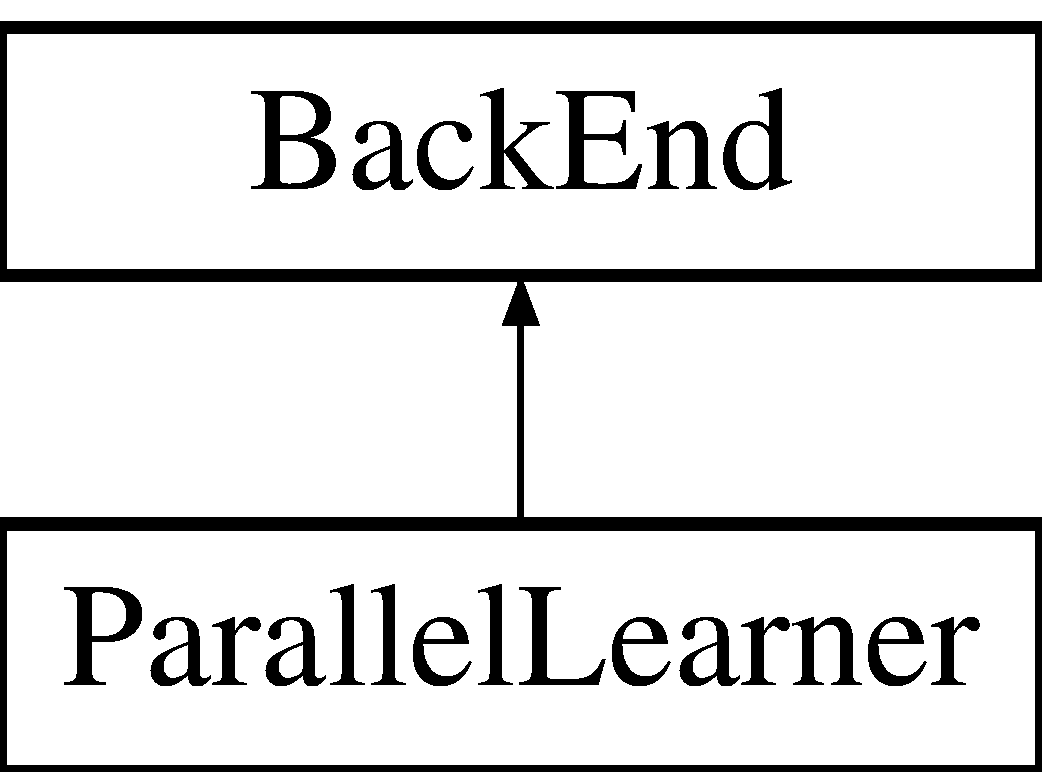
\includegraphics[height=2.000000cm]{classParallelLearner}
\end{center}
\end{figure}
\subsection*{Public Member Functions}
\begin{DoxyCompactItemize}
\item 
\hyperlink{classParallelLearner_a469e826d756c7c1a932128cfb17ce380}{Parallel\-Learner} (size\-\_\-t nr\-\_\-of\-\_\-threads)
\begin{DoxyCompactList}\small\item\em Constructor. \end{DoxyCompactList}\item 
virtual \hyperlink{classParallelLearner_a42d85a531cab28bdcb345c37a0b08730}{$\sim$\-Parallel\-Learner} ()
\begin{DoxyCompactList}\small\item\em Desctructor. \end{DoxyCompactList}\item 
virtual bool \hyperlink{classParallelLearner_a93acb74e7c8504d0ef2bd3697441b745}{run} ()
\begin{DoxyCompactList}\small\item\em Runs the back-\/end. \end{DoxyCompactList}\item 
void \hyperlink{classParallelLearner_a10b8346745051c95f05a1bc8356fcf8d}{notify\-New\-Win\-Reg\-Clause} (const vector$<$ int $>$ \&clause, int src)
\begin{DoxyCompactList}\small\item\em Notifies all worker-\/threads that a new clause of the winning region is available. \end{DoxyCompactList}\item 
void \hyperlink{classParallelLearner_a0a8405e4fb7331f3f3df2711fdaebdab}{notify\-New\-Useless\-Input\-Clause} (const vector$<$ int $>$ \&clause, int level)
\begin{DoxyCompactList}\small\item\em Notifies all Clause\-Explorer\-S\-A\-T-\/threads that a new U-\/clause is available. \end{DoxyCompactList}\item 
void \hyperlink{classParallelLearner_a8c59cc455059943f8f9cdb8a60526f5c}{notify\-New\-Counterexample} (const vector$<$ int $>$ \&ce, const vector$<$ int $>$ \&gen)
\begin{DoxyCompactList}\small\item\em Adds a new counterexample to the \hyperlink{classParallelLearner}{Parallel\-Learner}'s database. \end{DoxyCompactList}\item 
void \hyperlink{classParallelLearner_a2b8e4330afb7e99c19d2d7da15c30cc3}{trigger\-Explorer\-Restart} ()
\begin{DoxyCompactList}\small\item\em Computes a new restart point and notifies it to all Clause\-Explorer\-S\-A\-T-\/instances. \end{DoxyCompactList}\end{DoxyCompactItemize}
\subsection*{Public Attributes}
\begin{DoxyCompactItemize}
\item 
int \hyperlink{classParallelLearner_a757f8817809cce5c0408cdc41d6db1b8}{result\-\_\-}
\begin{DoxyCompactList}\small\item\em An integer number containing the realizability verdict. \end{DoxyCompactList}\item 
\hyperlink{classCNF}{C\-N\-F} \hyperlink{classParallelLearner_a7c8383543ff98d7a0356a237756dcdd6}{winning\-\_\-region\-\_\-}
\begin{DoxyCompactList}\small\item\em The current version of the winning region. \end{DoxyCompactList}\item 
mutex \hyperlink{classParallelLearner_a196a4500dfd66a4b9110659b4a10dead}{winning\-\_\-region\-\_\-lock\-\_\-}
\begin{DoxyCompactList}\small\item\em A lock that protects the \hyperlink{classParallelLearner_a7c8383543ff98d7a0356a237756dcdd6}{winning\-\_\-region\-\_\-} from race-\/conditions. \end{DoxyCompactList}\item 
\hyperlink{classCNF}{C\-N\-F} \hyperlink{classParallelLearner_aba6b363071d9a39d7b368cec5b629c25}{unminimized\-\_\-clauses\-\_\-}
\begin{DoxyCompactList}\small\item\em All clauses of the winning region that have not yet been minimized. \end{DoxyCompactList}\item 
mutex \hyperlink{classParallelLearner_aa16d364d9fdd0c2fe5180ee1b023a4ec}{unminimized\-\_\-clauses\-\_\-lock\-\_\-}
\begin{DoxyCompactList}\small\item\em A lock that protects the \hyperlink{classParallelLearner_aba6b363071d9a39d7b368cec5b629c25}{unminimized\-\_\-clauses\-\_\-} from race-\/conditions. \end{DoxyCompactList}\item 
list$<$ pair$<$ vector$<$ int $>$\\*
, vector$<$ int $>$ $>$ $>$ \hyperlink{classParallelLearner_a974943e3e2145b3407f689b64acdd33f}{counterexamples\-\_\-}
\begin{DoxyCompactList}\small\item\em The counterexample-\/cubes together with their computed generalizations. \end{DoxyCompactList}\item 
mutex \hyperlink{classParallelLearner_a454c81908f2d3cb4c24b042739adc4ec}{counterexamples\-\_\-lock\-\_\-}
\begin{DoxyCompactList}\small\item\em A lock that protects the \hyperlink{classParallelLearner_a974943e3e2145b3407f689b64acdd33f}{counterexamples\-\_\-} from race-\/conditions. \end{DoxyCompactList}\item 
mutex \hyperlink{classParallelLearner_abdd409a5ef29bd4ba6b7213e9d4a067b}{var\-\_\-man\-\_\-lock\-\_\-}
\begin{DoxyCompactList}\small\item\em A lock that must be hold when the \hyperlink{classVarManager}{Var\-Manager} is modified. \end{DoxyCompactList}\end{DoxyCompactItemize}
\subsection*{Static Public Attributes}
\begin{DoxyCompactItemize}
\item 
static mutex \hyperlink{classParallelLearner_a5bc71a2c35fa976d792bf0e80de31a39}{print\-\_\-lock\-\_\-}
\begin{DoxyCompactList}\small\item\em A lock used to synchronize the printing of debugging messages. \end{DoxyCompactList}\end{DoxyCompactItemize}
\subsection*{Protected Member Functions}
\begin{DoxyCompactItemize}
\item 
void \hyperlink{classParallelLearner_a2b87f1f2526786a4402d695026272d33}{compute\-Previous\-Trans} ()
\begin{DoxyCompactList}\small\item\em A helper function to compute the previous-\/state copy of the transition relation. \end{DoxyCompactList}\item 
int \hyperlink{classParallelLearner_aa97595b50d1bba411824c2a60337e081}{present\-To\-Previous} (int literal) const 
\begin{DoxyCompactList}\small\item\em Returns the previous-\/state copy of a literal. \end{DoxyCompactList}\item 
void \hyperlink{classParallelLearner_ae3330a141c8ba3ca7c5687824dbf4edc}{present\-To\-Previous} (vector$<$ int $>$ \&cube\-\_\-or\-\_\-clause) const 
\begin{DoxyCompactList}\small\item\em Computes the previous-\/state copy of a cube or clause. \end{DoxyCompactList}\item 
void \hyperlink{classParallelLearner_acce71499ce9d8672116139f231376151}{present\-To\-Previous} (\hyperlink{classCNF}{C\-N\-F} \&cnf) const 
\begin{DoxyCompactList}\small\item\em Computes the previous-\/state copy of a \hyperlink{classCNF}{C\-N\-F}. \end{DoxyCompactList}\end{DoxyCompactItemize}
\subsection*{Protected Attributes}
\begin{DoxyCompactItemize}
\item 
bool \hyperlink{classParallelLearner_aebaf891aada574da650732795f041dbe}{use\-\_\-ind\-\_\-}
\begin{DoxyCompactList}\small\item\em A flag indicating if optimization R\-G should be used. \end{DoxyCompactList}\item 
size\-\_\-t \hyperlink{classParallelLearner_a170a0abad017845877039684507e7a66}{nr\-\_\-of\-\_\-threads\-\_\-}
\begin{DoxyCompactList}\small\item\em The number of threads to instantiate and execute. \end{DoxyCompactList}\item 
vector$<$ \hyperlink{classClauseExplorerSAT}{Clause\-Explorer\-S\-A\-T} $\ast$ $>$ \hyperlink{classParallelLearner_a0e8b5dd12c8ae14089d3ce3117da3c16}{clause\-\_\-explorers\-\_\-}
\begin{DoxyCompactList}\small\item\em The Clause\-Explorer\-S\-A\-T-\/instances to execute in a separate thread. \end{DoxyCompactList}\item 
vector$<$ \hyperlink{classIFM13Explorer}{I\-F\-M13\-Explorer} $\ast$ $>$ \hyperlink{classParallelLearner_a614707a21f36d75a9fd06be57ee421d0}{ifm\-\_\-explorers\-\_\-}
\begin{DoxyCompactList}\small\item\em The I\-F\-M13\-Explorer-\/instances to execute in a separate thread. \end{DoxyCompactList}\item 
vector$<$ \hyperlink{classClauseMinimizerQBF}{Clause\-Minimizer\-Q\-B\-F} $\ast$ $>$ \hyperlink{classParallelLearner_adb5aa1e016e04c607073eaf90d994dc7}{clause\-\_\-minimizers\-\_\-}
\begin{DoxyCompactList}\small\item\em The Clause\-Minimizer\-Q\-B\-F-\/instances to execute in a separate thread. \end{DoxyCompactList}\item 
vector$<$ \hyperlink{classCounterGenSAT}{Counter\-Gen\-S\-A\-T} $\ast$ $>$ \hyperlink{classParallelLearner_a46cc16764d7ea8ffafe8d1b696c35df3}{ce\-\_\-generalizers\-\_\-}
\begin{DoxyCompactList}\small\item\em The Counter\-Gen\-S\-A\-T-\/instances to execute in a separate thread. \end{DoxyCompactList}\item 
\hyperlink{classLearnStatisticsSAT}{Learn\-Statistics\-S\-A\-T} \hyperlink{classParallelLearner_abfb2e28ec1a0f8775d3f14f75415a8bd}{statistics\-\_\-}
\begin{DoxyCompactList}\small\item\em Stores and maintains statistics and performance measures. \end{DoxyCompactList}\item 
\hyperlink{classCNF}{C\-N\-F} \hyperlink{classParallelLearner_ac73d9338262855f61f23a65d1df0647c}{prev\-\_\-trans\-\_\-or\-\_\-initial\-\_\-}
\begin{DoxyCompactList}\small\item\em Says\-: the current state is initial or the previous transition relation holds. \end{DoxyCompactList}\item 
vector$<$ int $>$ \hyperlink{classParallelLearner_a6f8dfda6aa8640345057023ed85882b9}{current\-\_\-to\-\_\-previous\-\_\-map\-\_\-}
\begin{DoxyCompactList}\small\item\em A map from present-\/state variables to their previous-\/state copy. \end{DoxyCompactList}\item 
int \hyperlink{classParallelLearner_ae9293a4afd3c52690bcac2ad03884121}{current\-\_\-state\-\_\-is\-\_\-initial\-\_\-}
\begin{DoxyCompactList}\small\item\em A literal that is true if the current state is initial and false otherwise. \end{DoxyCompactList}\end{DoxyCompactItemize}
\subsection*{Private Member Functions}
\begin{DoxyCompactItemize}
\item 
\hyperlink{classParallelLearner_a7857993d63e497f5c946030c3127a578}{Parallel\-Learner} (const \hyperlink{classParallelLearner}{Parallel\-Learner} \&other)
\begin{DoxyCompactList}\small\item\em Copy constructor. \end{DoxyCompactList}\item 
\hyperlink{classParallelLearner}{Parallel\-Learner} \& \hyperlink{classParallelLearner_a870e6d78e50b8aed63555e797ff6cce4}{operator=} (const \hyperlink{classParallelLearner}{Parallel\-Learner} \&other)
\begin{DoxyCompactList}\small\item\em Assignment operator. \end{DoxyCompactList}\end{DoxyCompactItemize}


\subsection{Detailed Description}
The coordinator of the parallelized implementation. 

This class implements a parallelized version of the learning-\/based synthesis methods. The idea is to combine various different techniques to refine an over-\/approximation of the winning region with new clauses. There is a lot of flexibility to play with. We can have threads discovering new clauses with S\-A\-T-\/ or Q\-B\-F-\/based learning techniques, we can have threads minimizing existing clauses with a Q\-B\-F solver, etc. All threads share a common clause database. If (new or refined) clauses are discovered, they are communicated to all threads such that all of them can benefit from the new clauses in the next call. The threads performing actual work are implemented in other classes. This class is just the coordinator which starts the worker-\/threads and forwards information about new clauses to the worker-\/threads.

The parallel implementation has two advantages. First, it exploits hardware parallelism (modern C\-P\-Us have many cores), which means (potentially) shorter computation times. Second, it is an easy way of combining different methods. With one thread, one would have come up with points where to switch from one method to the other and back. Hence, it may also be useful to use the parallelized implementation even if only one core is available.

The question which methods we should combine how in order to achieve the best speed-\/up is not yet fully solved. This class is just one attempt, and can be seen as a playground for combining different methods.

\begin{DoxyAuthor}{Author}
Robert Koenighofer (\href{mailto:robert.koenighofer@iaik.tugraz.at}{\tt robert.\-koenighofer@iaik.\-tugraz.\-at}) 
\end{DoxyAuthor}
\begin{DoxyVersion}{Version}
1.\-0.\-0 
\end{DoxyVersion}


Definition at line 77 of file Parallel\-Learner.\-h.



\subsection{Constructor \& Destructor Documentation}
\hypertarget{classParallelLearner_a469e826d756c7c1a932128cfb17ce380}{\index{Parallel\-Learner@{Parallel\-Learner}!Parallel\-Learner@{Parallel\-Learner}}
\index{Parallel\-Learner@{Parallel\-Learner}!ParallelLearner@{Parallel\-Learner}}
\subsubsection[{Parallel\-Learner}]{\setlength{\rightskip}{0pt plus 5cm}Parallel\-Learner\-::\-Parallel\-Learner (
\begin{DoxyParamCaption}
\item[{size\-\_\-t}]{nr\-\_\-of\-\_\-threads}
\end{DoxyParamCaption}
)}}\label{classParallelLearner_a469e826d756c7c1a932128cfb17ce380}


Constructor. 


\begin{DoxyParams}{Parameters}
{\em nr\-\_\-of\-\_\-threads} & The number of threads to create. This does not have to be the number of cores in your C\-P\-U. It can also make sense to combine several methods running in several threads on one single core. The methods can complement each other and achieve a speedup compared to one single method in isolation. \\
\hline
\end{DoxyParams}


Definition at line 116 of file Parallel\-Learner.\-cpp.



References ce\-\_\-generalizers\-\_\-, clause\-\_\-explorers\-\_\-, clause\-\_\-minimizers\-\_\-, compute\-Previous\-Trans(), current\-\_\-state\-\_\-is\-\_\-initial\-\_\-, current\-\_\-to\-\_\-previous\-\_\-map\-\_\-, Options\-::get\-Back\-End\-Mode(), ifm\-\_\-explorers\-\_\-, Options\-::instance(), M\-A\-S\-S\-E\-R\-T, prev\-\_\-trans\-\_\-or\-\_\-initial\-\_\-, and use\-\_\-ind\-\_\-.

\hypertarget{classParallelLearner_a42d85a531cab28bdcb345c37a0b08730}{\index{Parallel\-Learner@{Parallel\-Learner}!$\sim$\-Parallel\-Learner@{$\sim$\-Parallel\-Learner}}
\index{$\sim$\-Parallel\-Learner@{$\sim$\-Parallel\-Learner}!ParallelLearner@{Parallel\-Learner}}
\subsubsection[{$\sim$\-Parallel\-Learner}]{\setlength{\rightskip}{0pt plus 5cm}Parallel\-Learner\-::$\sim$\-Parallel\-Learner (
\begin{DoxyParamCaption}
{}
\end{DoxyParamCaption}
)\hspace{0.3cm}{\ttfamily [virtual]}}}\label{classParallelLearner_a42d85a531cab28bdcb345c37a0b08730}


Desctructor. 



Definition at line 225 of file Parallel\-Learner.\-cpp.



References ce\-\_\-generalizers\-\_\-, clause\-\_\-explorers\-\_\-, clause\-\_\-minimizers\-\_\-, and ifm\-\_\-explorers\-\_\-.

\hypertarget{classParallelLearner_a7857993d63e497f5c946030c3127a578}{\index{Parallel\-Learner@{Parallel\-Learner}!Parallel\-Learner@{Parallel\-Learner}}
\index{Parallel\-Learner@{Parallel\-Learner}!ParallelLearner@{Parallel\-Learner}}
\subsubsection[{Parallel\-Learner}]{\setlength{\rightskip}{0pt plus 5cm}Parallel\-Learner\-::\-Parallel\-Learner (
\begin{DoxyParamCaption}
\item[{const {\bf Parallel\-Learner} \&}]{other}
\end{DoxyParamCaption}
)\hspace{0.3cm}{\ttfamily [private]}}}\label{classParallelLearner_a7857993d63e497f5c946030c3127a578}


Copy constructor. 

The copy constructor is disabled (set private) and not implemented.


\begin{DoxyParams}{Parameters}
{\em other} & The source for creating the copy. \\
\hline
\end{DoxyParams}


\subsection{Member Function Documentation}
\hypertarget{classParallelLearner_a2b87f1f2526786a4402d695026272d33}{\index{Parallel\-Learner@{Parallel\-Learner}!compute\-Previous\-Trans@{compute\-Previous\-Trans}}
\index{compute\-Previous\-Trans@{compute\-Previous\-Trans}!ParallelLearner@{Parallel\-Learner}}
\subsubsection[{compute\-Previous\-Trans}]{\setlength{\rightskip}{0pt plus 5cm}void Parallel\-Learner\-::compute\-Previous\-Trans (
\begin{DoxyParamCaption}
{}
\end{DoxyParamCaption}
)\hspace{0.3cm}{\ttfamily [protected]}}}\label{classParallelLearner_a2b87f1f2526786a4402d695026272d33}


A helper function to compute the previous-\/state copy of the transition relation. 

This is needed if optimization R\-G is enabled (see \hyperlink{classLearnSynthQBFInd}{Learn\-Synth\-Q\-B\-F\-Ind}). 

Definition at line 405 of file Parallel\-Learner.\-cpp.



References C\-N\-F\-::add2\-Lit\-Clause(), Var\-Manager\-::create\-Fresh\-Prev\-Var(), Var\-Manager\-::create\-Fresh\-Tmp\-Var(), Var\-Info\-::\-C\-T\-R\-L, current\-\_\-state\-\_\-is\-\_\-initial\-\_\-, current\-\_\-to\-\_\-previous\-\_\-map\-\_\-, C\-N\-F\-::get\-Clauses(), Var\-Manager\-::get\-Max\-C\-N\-F\-Var(), A\-I\-G2\-C\-N\-F\-::get\-Trans(), Var\-Manager\-::get\-Vars\-Of\-Type(), Var\-Info\-::\-I\-N\-P\-U\-T, Var\-Manager\-::instance(), A\-I\-G2\-C\-N\-F\-::instance(), Var\-Info\-::\-N\-E\-X\-T\-\_\-\-S\-T\-A\-T\-E, Var\-Info\-::\-P\-R\-E\-S\-\_\-\-S\-T\-A\-T\-E, present\-To\-Previous(), prev\-\_\-trans\-\_\-or\-\_\-initial\-\_\-, C\-N\-F\-::swap\-With(), and Var\-Info\-::\-T\-M\-P.



Referenced by Parallel\-Learner().

\hypertarget{classParallelLearner_a8c59cc455059943f8f9cdb8a60526f5c}{\index{Parallel\-Learner@{Parallel\-Learner}!notify\-New\-Counterexample@{notify\-New\-Counterexample}}
\index{notify\-New\-Counterexample@{notify\-New\-Counterexample}!ParallelLearner@{Parallel\-Learner}}
\subsubsection[{notify\-New\-Counterexample}]{\setlength{\rightskip}{0pt plus 5cm}void Parallel\-Learner\-::notify\-New\-Counterexample (
\begin{DoxyParamCaption}
\item[{const vector$<$ int $>$ \&}]{ce, }
\item[{const vector$<$ int $>$ \&}]{gen}
\end{DoxyParamCaption}
)}}\label{classParallelLearner_a8c59cc455059943f8f9cdb8a60526f5c}


Adds a new counterexample to the \hyperlink{classParallelLearner}{Parallel\-Learner}'s database. 

A counterexample is a state-\/input combination with which the antagonist can enforce to leave the winning region. The counterexample is stored together with a generalization (some literals dropped) that has already been computed. This information can then be used by Counter\-Gen\-S\-A\-T-\/threads. They take such a counterexample and compute all other generalizations (generalizations other than 'gen').


\begin{DoxyParams}{Parameters}
{\em ce} & This is a cube of the current-\/state variables and the uncontrollable inputs. With this state-\/input combination, the antagonist can enforce to leave the winning region. That is, there are no control-\/values such that the successor state is in the winning region again. \\
\hline
{\em gen} & One generalization of the counterexample. This is a subset of the literals of ce such that no control-\/values can lead to a successor state inside the winning region. \\
\hline
\end{DoxyParams}


Definition at line 368 of file Parallel\-Learner.\-cpp.



References ce\-\_\-generalizers\-\_\-, counterexamples\-\_\-, and counterexamples\-\_\-lock\-\_\-.



Referenced by Clause\-Explorer\-S\-A\-T\-::explore\-Clauses().

\hypertarget{classParallelLearner_a0a8405e4fb7331f3f3df2711fdaebdab}{\index{Parallel\-Learner@{Parallel\-Learner}!notify\-New\-Useless\-Input\-Clause@{notify\-New\-Useless\-Input\-Clause}}
\index{notify\-New\-Useless\-Input\-Clause@{notify\-New\-Useless\-Input\-Clause}!ParallelLearner@{Parallel\-Learner}}
\subsubsection[{notify\-New\-Useless\-Input\-Clause}]{\setlength{\rightskip}{0pt plus 5cm}void Parallel\-Learner\-::notify\-New\-Useless\-Input\-Clause (
\begin{DoxyParamCaption}
\item[{const vector$<$ int $>$ \&}]{clause, }
\item[{int}]{level}
\end{DoxyParamCaption}
)}}\label{classParallelLearner_a0a8405e4fb7331f3f3df2711fdaebdab}


Notifies all Clause\-Explorer\-S\-A\-T-\/threads that a new U-\/clause is available. 

In essence, the \hyperlink{classClauseExplorerSAT}{Clause\-Explorer\-S\-A\-T} implements the same S\-A\-T-\/based learning method as \hyperlink{classLearnSynthSAT}{Learn\-Synth\-S\-A\-T}. It has just a few additional features which allow the implementation to communicate with others. A U-\/clause states that a certain state-\/input is useless for the antagonist in trying to leave the winning region (see \hyperlink{classLearnSynthSAT}{Learn\-Synth\-S\-A\-T} for details). If one \hyperlink{classClauseExplorerSAT}{Clause\-Explorer\-S\-A\-T} discovers such a clause, it communicates it to all other Clause\-Explorer\-S\-A\-T-\/instances such that they can also benefit from it and do not need to re-\/discover the same fact again. For that to work, all \hyperlink{classClauseExplorerSAT}{Clause\-Explorer\-S\-A\-T} must be synchronized to a certain extend\-: All \hyperlink{classClauseExplorerSAT}{Clause\-Explorer\-S\-A\-T} must do solver restarts simultaneously. We pass the restart-\/level (the number of restarts done so far) as additional parameter so that every Clause\-Explorer\-S\-A\-T-\/instances can then decide if this clause is helpful for him, or already out-\/dated.


\begin{DoxyParams}{Parameters}
{\em clause} & A new U-\/clause stating that a certain state-\/input is useless for the antagonist in trying to leave the winning region (see \hyperlink{classLearnSynthSAT}{Learn\-Synth\-S\-A\-T} for details). \\
\hline
{\em level} & The restart level (the number of solver restarts that have already been performed. This information allows the receiver instance to decide whether or not this clause is useful for her (or if it is already out-\/dated). \\
\hline
\end{DoxyParams}


Definition at line 356 of file Parallel\-Learner.\-cpp.



References clause\-\_\-explorers\-\_\-.



Referenced by Clause\-Explorer\-S\-A\-T\-::explore\-Clauses().

\hypertarget{classParallelLearner_a10b8346745051c95f05a1bc8356fcf8d}{\index{Parallel\-Learner@{Parallel\-Learner}!notify\-New\-Win\-Reg\-Clause@{notify\-New\-Win\-Reg\-Clause}}
\index{notify\-New\-Win\-Reg\-Clause@{notify\-New\-Win\-Reg\-Clause}!ParallelLearner@{Parallel\-Learner}}
\subsubsection[{notify\-New\-Win\-Reg\-Clause}]{\setlength{\rightskip}{0pt plus 5cm}void Parallel\-Learner\-::notify\-New\-Win\-Reg\-Clause (
\begin{DoxyParamCaption}
\item[{const vector$<$ int $>$ \&}]{clause, }
\item[{int}]{src}
\end{DoxyParamCaption}
)}}\label{classParallelLearner_a10b8346745051c95f05a1bc8356fcf8d}


Notifies all worker-\/threads that a new clause of the winning region is available. 

It also adds this clause to our global clause database \hyperlink{classParallelLearner_a7c8383543ff98d7a0356a237756dcdd6}{winning\-\_\-region\-\_\-}. 
\begin{DoxyParams}{Parameters}
{\em clause} & The new clause that has been discovered. \\
\hline
{\em src} & An integer number defining which kind of worker-\/thread discovered the clause. Some worker-\/threads may treat clauses from different sources in a special way. \\
\hline
\end{DoxyParams}


Definition at line 326 of file Parallel\-Learner.\-cpp.



References C\-N\-F\-::add\-Clause(), C\-N\-F\-::add\-Clause\-And\-Simplify(), ce\-\_\-generalizers\-\_\-, clause\-\_\-explorers\-\_\-, clause\-\_\-minimizers\-\_\-, ifm\-\_\-explorers\-\_\-, M\-I\-N, unminimized\-\_\-clauses\-\_\-, unminimized\-\_\-clauses\-\_\-lock\-\_\-, winning\-\_\-region\-\_\-, and winning\-\_\-region\-\_\-lock\-\_\-.



Referenced by I\-F\-M13\-Explorer\-::add\-Lose(), Counter\-Gen\-S\-A\-T\-::bored(), Clause\-Explorer\-S\-A\-T\-::explore\-Clauses(), Counter\-Gen\-S\-A\-T\-::generalize\-Counterexamples(), and Clause\-Minimizer\-Q\-B\-F\-::minimize\-Clauses().

\hypertarget{classParallelLearner_a870e6d78e50b8aed63555e797ff6cce4}{\index{Parallel\-Learner@{Parallel\-Learner}!operator=@{operator=}}
\index{operator=@{operator=}!ParallelLearner@{Parallel\-Learner}}
\subsubsection[{operator=}]{\setlength{\rightskip}{0pt plus 5cm}{\bf Parallel\-Learner}\& Parallel\-Learner\-::operator= (
\begin{DoxyParamCaption}
\item[{const {\bf Parallel\-Learner} \&}]{other}
\end{DoxyParamCaption}
)\hspace{0.3cm}{\ttfamily [private]}}}\label{classParallelLearner_a870e6d78e50b8aed63555e797ff6cce4}


Assignment operator. 

The assignment operator is disabled (set private) and not implemented.


\begin{DoxyParams}{Parameters}
{\em other} & The source for creating the copy. \\
\hline
\end{DoxyParams}
\begin{DoxyReturn}{Returns}
The result of the assignment, i.\-e, $\ast$this. 
\end{DoxyReturn}
\hypertarget{classParallelLearner_aa97595b50d1bba411824c2a60337e081}{\index{Parallel\-Learner@{Parallel\-Learner}!present\-To\-Previous@{present\-To\-Previous}}
\index{present\-To\-Previous@{present\-To\-Previous}!ParallelLearner@{Parallel\-Learner}}
\subsubsection[{present\-To\-Previous}]{\setlength{\rightskip}{0pt plus 5cm}int Parallel\-Learner\-::present\-To\-Previous (
\begin{DoxyParamCaption}
\item[{int}]{literal}
\end{DoxyParamCaption}
) const\hspace{0.3cm}{\ttfamily [protected]}}}\label{classParallelLearner_aa97595b50d1bba411824c2a60337e081}


Returns the previous-\/state copy of a literal. 


\begin{DoxyParams}{Parameters}
{\em literal} & The literal to transform. \\
\hline
\end{DoxyParams}
\begin{DoxyReturn}{Returns}
The previous-\/state copy of a literal. 
\end{DoxyReturn}


Definition at line 442 of file Parallel\-Learner.\-cpp.



References current\-\_\-to\-\_\-previous\-\_\-map\-\_\-.



Referenced by compute\-Previous\-Trans(), and present\-To\-Previous().

\hypertarget{classParallelLearner_ae3330a141c8ba3ca7c5687824dbf4edc}{\index{Parallel\-Learner@{Parallel\-Learner}!present\-To\-Previous@{present\-To\-Previous}}
\index{present\-To\-Previous@{present\-To\-Previous}!ParallelLearner@{Parallel\-Learner}}
\subsubsection[{present\-To\-Previous}]{\setlength{\rightskip}{0pt plus 5cm}void Parallel\-Learner\-::present\-To\-Previous (
\begin{DoxyParamCaption}
\item[{vector$<$ int $>$ \&}]{cube\-\_\-or\-\_\-clause}
\end{DoxyParamCaption}
) const\hspace{0.3cm}{\ttfamily [protected]}}}\label{classParallelLearner_ae3330a141c8ba3ca7c5687824dbf4edc}


Computes the previous-\/state copy of a cube or clause. 


\begin{DoxyParams}{Parameters}
{\em cube\-\_\-or\-\_\-clause} & A cube or clause (in form of a vector of literals) over the present state variables. This vector is overwritten by the corresponding cube of clause over the previous-\/state literals (i.\-e., all literals are replaced by their previous-\/state copy). \\
\hline
\end{DoxyParams}


Definition at line 452 of file Parallel\-Learner.\-cpp.



References present\-To\-Previous().

\hypertarget{classParallelLearner_acce71499ce9d8672116139f231376151}{\index{Parallel\-Learner@{Parallel\-Learner}!present\-To\-Previous@{present\-To\-Previous}}
\index{present\-To\-Previous@{present\-To\-Previous}!ParallelLearner@{Parallel\-Learner}}
\subsubsection[{present\-To\-Previous}]{\setlength{\rightskip}{0pt plus 5cm}void Parallel\-Learner\-::present\-To\-Previous (
\begin{DoxyParamCaption}
\item[{{\bf C\-N\-F} \&}]{cnf}
\end{DoxyParamCaption}
) const\hspace{0.3cm}{\ttfamily [protected]}}}\label{classParallelLearner_acce71499ce9d8672116139f231376151}


Computes the previous-\/state copy of a \hyperlink{classCNF}{C\-N\-F}. 


\begin{DoxyParams}{Parameters}
{\em cnf} & A \hyperlink{classCNF}{C\-N\-F} formula over the present state variables. This \hyperlink{classCNF}{C\-N\-F} is overwritten by the corresponding \hyperlink{classCNF}{C\-N\-F} over the previous-\/state literals (i.\-e., all literals are replaced by their previous-\/state copy). \\
\hline
\end{DoxyParams}


Definition at line 459 of file Parallel\-Learner.\-cpp.



References C\-N\-F\-::add\-Clause(), C\-N\-F\-::clear(), C\-N\-F\-::get\-Clauses(), and present\-To\-Previous().

\hypertarget{classParallelLearner_a93acb74e7c8504d0ef2bd3697441b745}{\index{Parallel\-Learner@{Parallel\-Learner}!run@{run}}
\index{run@{run}!ParallelLearner@{Parallel\-Learner}}
\subsubsection[{run}]{\setlength{\rightskip}{0pt plus 5cm}bool Parallel\-Learner\-::run (
\begin{DoxyParamCaption}
{}
\end{DoxyParamCaption}
)\hspace{0.3cm}{\ttfamily [virtual]}}}\label{classParallelLearner_a93acb74e7c8504d0ef2bd3697441b745}


Runs the back-\/end. 

This method mainly starts the worker-\/threads and waits until they are finished. The \hyperlink{classParallelLearner}{Parallel\-Learner} itself does not do any work. It does not even run in an own thread. All the work is done in the worker-\/threads.

\begin{DoxyReturn}{Returns}
True if the specification was realizable, false otherwise. 
\end{DoxyReturn}


Implements \hyperlink{classBackEnd_a099e717dc71e9cc2d838b1ca86340590}{Back\-End}.



Definition at line 245 of file Parallel\-Learner.\-cpp.



References C\-N\-F\-::add\-C\-N\-F(), ce\-\_\-generalizers\-\_\-, clause\-\_\-explorers\-\_\-, clause\-\_\-minimizers\-\_\-, C\-N\-F\-::clear(), Utils\-::debug\-Check\-Win\-Reg(), Clause\-Explorer\-S\-A\-T\-::explore\-Clauses(), I\-F\-M13\-Explorer\-::explore\-Clauses(), Q\-B\-F\-Cert\-Impl\-Extractor\-::extract\-Circuit(), Counter\-Gen\-S\-A\-T\-::generalize\-Counterexamples(), ifm\-\_\-explorers\-\_\-, Var\-Manager\-::instance(), Options\-::instance(), A\-I\-G2\-C\-N\-F\-::instance(), L\-\_\-\-I\-N\-F, L\-\_\-\-R\-E\-S, Learn\-Statistics\-S\-A\-T\-::log\-Statistics(), M\-A\-S\-S\-E\-R\-T, Learn\-Statistics\-S\-A\-T\-::merge\-With(), Clause\-Minimizer\-Q\-B\-F\-::minimize\-Clauses(), Learn\-Statistics\-S\-A\-T\-::notify\-Rel\-Det\-End(), Learn\-Statistics\-S\-A\-T\-::notify\-Rel\-Det\-Start(), Learn\-Statistics\-S\-A\-T\-::notify\-Win\-Reg\-End(), Learn\-Statistics\-S\-A\-T\-::notify\-Win\-Reg\-Start(), nr\-\_\-of\-\_\-threads\-\_\-, Var\-Manager\-::push(), result\-\_\-, statistics\-\_\-, U\-N\-R\-E\-A\-L\-I\-Z\-A\-B\-L\-E, and winning\-\_\-region\-\_\-.

\hypertarget{classParallelLearner_a2b8e4330afb7e99c19d2d7da15c30cc3}{\index{Parallel\-Learner@{Parallel\-Learner}!trigger\-Explorer\-Restart@{trigger\-Explorer\-Restart}}
\index{trigger\-Explorer\-Restart@{trigger\-Explorer\-Restart}!ParallelLearner@{Parallel\-Learner}}
\subsubsection[{trigger\-Explorer\-Restart}]{\setlength{\rightskip}{0pt plus 5cm}void Parallel\-Learner\-::trigger\-Explorer\-Restart (
\begin{DoxyParamCaption}
{}
\end{DoxyParamCaption}
)}}\label{classParallelLearner_a2b8e4330afb7e99c19d2d7da15c30cc3}


Computes a new restart point and notifies it to all Clause\-Explorer\-S\-A\-T-\/instances. 

The \hyperlink{classClauseExplorerSAT}{Clause\-Explorer\-S\-A\-T} update their next-\/state copy of the winning region only in a lazy manner. This allows them to use incremental S\-A\-T-\/solving more effectively. See \hyperlink{classLearnSynthSAT}{Learn\-Synth\-S\-A\-T} for a description. If no more solutions exists with one next-\/state copy of the winning region, it must be updated to the newest version. This is done by this method. A new next-\/state copy of the winning region is computed and communicated to all Clause\-Explorer\-S\-A\-T-\/instances. It is absolutely important that all \hyperlink{classClauseExplorerSAT}{Clause\-Explorer\-S\-A\-T} instances work with the same next-\/state copy of the winning region. Otherwise, they could not exchange U-\/clauses (or rather, the U-\/clause discovered by one thread would not make sense for the other). See also \hyperlink{classParallelLearner_a0a8405e4fb7331f3f3df2711fdaebdab}{notify\-New\-Useless\-Input\-Clause()}. 

Definition at line 379 of file Parallel\-Learner.\-cpp.



References C\-N\-F\-::add\-C\-N\-F(), clause\-\_\-explorers\-\_\-, Utils\-::compress\-State\-C\-N\-F(), Var\-Manager\-::instance(), A\-I\-G2\-C\-N\-F\-::instance(), C\-N\-F\-::negate(), Var\-Manager\-::reset\-To\-Last\-Push(), C\-N\-F\-::swap\-Present\-To\-Next(), var\-\_\-man\-\_\-lock\-\_\-, winning\-\_\-region\-\_\-, and winning\-\_\-region\-\_\-lock\-\_\-.



Referenced by Clause\-Explorer\-S\-A\-T\-::explore\-Clauses().



\subsection{Member Data Documentation}
\hypertarget{classParallelLearner_a46cc16764d7ea8ffafe8d1b696c35df3}{\index{Parallel\-Learner@{Parallel\-Learner}!ce\-\_\-generalizers\-\_\-@{ce\-\_\-generalizers\-\_\-}}
\index{ce\-\_\-generalizers\-\_\-@{ce\-\_\-generalizers\-\_\-}!ParallelLearner@{Parallel\-Learner}}
\subsubsection[{ce\-\_\-generalizers\-\_\-}]{\setlength{\rightskip}{0pt plus 5cm}vector$<${\bf Counter\-Gen\-S\-A\-T}$\ast$$>$ Parallel\-Learner\-::ce\-\_\-generalizers\-\_\-\hspace{0.3cm}{\ttfamily [protected]}}}\label{classParallelLearner_a46cc16764d7ea8ffafe8d1b696c35df3}


The Counter\-Gen\-S\-A\-T-\/instances to execute in a separate thread. 



Definition at line 330 of file Parallel\-Learner.\-h.



Referenced by notify\-New\-Counterexample(), notify\-New\-Win\-Reg\-Clause(), Parallel\-Learner(), run(), and $\sim$\-Parallel\-Learner().

\hypertarget{classParallelLearner_a0e8b5dd12c8ae14089d3ce3117da3c16}{\index{Parallel\-Learner@{Parallel\-Learner}!clause\-\_\-explorers\-\_\-@{clause\-\_\-explorers\-\_\-}}
\index{clause\-\_\-explorers\-\_\-@{clause\-\_\-explorers\-\_\-}!ParallelLearner@{Parallel\-Learner}}
\subsubsection[{clause\-\_\-explorers\-\_\-}]{\setlength{\rightskip}{0pt plus 5cm}vector$<${\bf Clause\-Explorer\-S\-A\-T}$\ast$$>$ Parallel\-Learner\-::clause\-\_\-explorers\-\_\-\hspace{0.3cm}{\ttfamily [protected]}}}\label{classParallelLearner_a0e8b5dd12c8ae14089d3ce3117da3c16}


The Clause\-Explorer\-S\-A\-T-\/instances to execute in a separate thread. 



Definition at line 315 of file Parallel\-Learner.\-h.



Referenced by notify\-New\-Useless\-Input\-Clause(), notify\-New\-Win\-Reg\-Clause(), Parallel\-Learner(), run(), trigger\-Explorer\-Restart(), and $\sim$\-Parallel\-Learner().

\hypertarget{classParallelLearner_adb5aa1e016e04c607073eaf90d994dc7}{\index{Parallel\-Learner@{Parallel\-Learner}!clause\-\_\-minimizers\-\_\-@{clause\-\_\-minimizers\-\_\-}}
\index{clause\-\_\-minimizers\-\_\-@{clause\-\_\-minimizers\-\_\-}!ParallelLearner@{Parallel\-Learner}}
\subsubsection[{clause\-\_\-minimizers\-\_\-}]{\setlength{\rightskip}{0pt plus 5cm}vector$<${\bf Clause\-Minimizer\-Q\-B\-F}$\ast$$>$ Parallel\-Learner\-::clause\-\_\-minimizers\-\_\-\hspace{0.3cm}{\ttfamily [protected]}}}\label{classParallelLearner_adb5aa1e016e04c607073eaf90d994dc7}


The Clause\-Minimizer\-Q\-B\-F-\/instances to execute in a separate thread. 



Definition at line 325 of file Parallel\-Learner.\-h.



Referenced by notify\-New\-Win\-Reg\-Clause(), Parallel\-Learner(), run(), and $\sim$\-Parallel\-Learner().

\hypertarget{classParallelLearner_a974943e3e2145b3407f689b64acdd33f}{\index{Parallel\-Learner@{Parallel\-Learner}!counterexamples\-\_\-@{counterexamples\-\_\-}}
\index{counterexamples\-\_\-@{counterexamples\-\_\-}!ParallelLearner@{Parallel\-Learner}}
\subsubsection[{counterexamples\-\_\-}]{\setlength{\rightskip}{0pt plus 5cm}list$<$pair$<$vector$<$int$>$, vector$<$int$>$ $>$ $>$ Parallel\-Learner\-::counterexamples\-\_\-}}\label{classParallelLearner_a974943e3e2145b3407f689b64acdd33f}


The counterexample-\/cubes together with their computed generalizations. 

The first item of the pairs stored in this list is always the counterexample itself. The second item of the pair is the generalization that has already been computed.

A counterexample is a state-\/input combination with which the antagonist can enforce to leave the winning region. The generalization is a sub-\/cube of the counterexample. This information can then be used by Counter\-Gen\-S\-A\-T-\/threads. They take such a counterexample and compute all other generalizations. 

Definition at line 236 of file Parallel\-Learner.\-h.



Referenced by Counter\-Gen\-S\-A\-T\-::generalize\-Counterexamples(), and notify\-New\-Counterexample().

\hypertarget{classParallelLearner_a454c81908f2d3cb4c24b042739adc4ec}{\index{Parallel\-Learner@{Parallel\-Learner}!counterexamples\-\_\-lock\-\_\-@{counterexamples\-\_\-lock\-\_\-}}
\index{counterexamples\-\_\-lock\-\_\-@{counterexamples\-\_\-lock\-\_\-}!ParallelLearner@{Parallel\-Learner}}
\subsubsection[{counterexamples\-\_\-lock\-\_\-}]{\setlength{\rightskip}{0pt plus 5cm}mutex Parallel\-Learner\-::counterexamples\-\_\-lock\-\_\-}}\label{classParallelLearner_a454c81908f2d3cb4c24b042739adc4ec}


A lock that protects the \hyperlink{classParallelLearner_a974943e3e2145b3407f689b64acdd33f}{counterexamples\-\_\-} from race-\/conditions. 

Many worker-\/threads modify the \hyperlink{classParallelLearner_a974943e3e2145b3407f689b64acdd33f}{counterexamples\-\_\-} (add new ones). This lock ensures that only one thread is modifying the \hyperlink{classParallelLearner_a974943e3e2145b3407f689b64acdd33f}{counterexamples\-\_\-} at one time. 

Definition at line 244 of file Parallel\-Learner.\-h.



Referenced by Counter\-Gen\-S\-A\-T\-::generalize\-Counterexamples(), and notify\-New\-Counterexample().

\hypertarget{classParallelLearner_ae9293a4afd3c52690bcac2ad03884121}{\index{Parallel\-Learner@{Parallel\-Learner}!current\-\_\-state\-\_\-is\-\_\-initial\-\_\-@{current\-\_\-state\-\_\-is\-\_\-initial\-\_\-}}
\index{current\-\_\-state\-\_\-is\-\_\-initial\-\_\-@{current\-\_\-state\-\_\-is\-\_\-initial\-\_\-}!ParallelLearner@{Parallel\-Learner}}
\subsubsection[{current\-\_\-state\-\_\-is\-\_\-initial\-\_\-}]{\setlength{\rightskip}{0pt plus 5cm}int Parallel\-Learner\-::current\-\_\-state\-\_\-is\-\_\-initial\-\_\-\hspace{0.3cm}{\ttfamily [protected]}}}\label{classParallelLearner_ae9293a4afd3c52690bcac2ad03884121}


A literal that is true if the current state is initial and false otherwise. 

The clauses assigning the literal are part of \hyperlink{classParallelLearner_ac73d9338262855f61f23a65d1df0647c}{prev\-\_\-trans\-\_\-or\-\_\-initial\-\_\-}. 

Definition at line 358 of file Parallel\-Learner.\-h.



Referenced by compute\-Previous\-Trans(), and Parallel\-Learner().

\hypertarget{classParallelLearner_a6f8dfda6aa8640345057023ed85882b9}{\index{Parallel\-Learner@{Parallel\-Learner}!current\-\_\-to\-\_\-previous\-\_\-map\-\_\-@{current\-\_\-to\-\_\-previous\-\_\-map\-\_\-}}
\index{current\-\_\-to\-\_\-previous\-\_\-map\-\_\-@{current\-\_\-to\-\_\-previous\-\_\-map\-\_\-}!ParallelLearner@{Parallel\-Learner}}
\subsubsection[{current\-\_\-to\-\_\-previous\-\_\-map\-\_\-}]{\setlength{\rightskip}{0pt plus 5cm}vector$<$int$>$ Parallel\-Learner\-::current\-\_\-to\-\_\-previous\-\_\-map\-\_\-\hspace{0.3cm}{\ttfamily [protected]}}}\label{classParallelLearner_a6f8dfda6aa8640345057023ed85882b9}


A map from present-\/state variables to their previous-\/state copy. 



Definition at line 351 of file Parallel\-Learner.\-h.



Referenced by compute\-Previous\-Trans(), Parallel\-Learner(), and present\-To\-Previous().

\hypertarget{classParallelLearner_a614707a21f36d75a9fd06be57ee421d0}{\index{Parallel\-Learner@{Parallel\-Learner}!ifm\-\_\-explorers\-\_\-@{ifm\-\_\-explorers\-\_\-}}
\index{ifm\-\_\-explorers\-\_\-@{ifm\-\_\-explorers\-\_\-}!ParallelLearner@{Parallel\-Learner}}
\subsubsection[{ifm\-\_\-explorers\-\_\-}]{\setlength{\rightskip}{0pt plus 5cm}vector$<${\bf I\-F\-M13\-Explorer}$\ast$$>$ Parallel\-Learner\-::ifm\-\_\-explorers\-\_\-\hspace{0.3cm}{\ttfamily [protected]}}}\label{classParallelLearner_a614707a21f36d75a9fd06be57ee421d0}


The I\-F\-M13\-Explorer-\/instances to execute in a separate thread. 



Definition at line 320 of file Parallel\-Learner.\-h.



Referenced by notify\-New\-Win\-Reg\-Clause(), Parallel\-Learner(), run(), and $\sim$\-Parallel\-Learner().

\hypertarget{classParallelLearner_a170a0abad017845877039684507e7a66}{\index{Parallel\-Learner@{Parallel\-Learner}!nr\-\_\-of\-\_\-threads\-\_\-@{nr\-\_\-of\-\_\-threads\-\_\-}}
\index{nr\-\_\-of\-\_\-threads\-\_\-@{nr\-\_\-of\-\_\-threads\-\_\-}!ParallelLearner@{Parallel\-Learner}}
\subsubsection[{nr\-\_\-of\-\_\-threads\-\_\-}]{\setlength{\rightskip}{0pt plus 5cm}size\-\_\-t Parallel\-Learner\-::nr\-\_\-of\-\_\-threads\-\_\-\hspace{0.3cm}{\ttfamily [protected]}}}\label{classParallelLearner_a170a0abad017845877039684507e7a66}


The number of threads to instantiate and execute. 



Definition at line 310 of file Parallel\-Learner.\-h.



Referenced by run().

\hypertarget{classParallelLearner_ac73d9338262855f61f23a65d1df0647c}{\index{Parallel\-Learner@{Parallel\-Learner}!prev\-\_\-trans\-\_\-or\-\_\-initial\-\_\-@{prev\-\_\-trans\-\_\-or\-\_\-initial\-\_\-}}
\index{prev\-\_\-trans\-\_\-or\-\_\-initial\-\_\-@{prev\-\_\-trans\-\_\-or\-\_\-initial\-\_\-}!ParallelLearner@{Parallel\-Learner}}
\subsubsection[{prev\-\_\-trans\-\_\-or\-\_\-initial\-\_\-}]{\setlength{\rightskip}{0pt plus 5cm}{\bf C\-N\-F} Parallel\-Learner\-::prev\-\_\-trans\-\_\-or\-\_\-initial\-\_\-\hspace{0.3cm}{\ttfamily [protected]}}}\label{classParallelLearner_ac73d9338262855f61f23a65d1df0647c}


Says\-: the current state is initial or the previous transition relation holds. 

This \hyperlink{classCNF}{C\-N\-F} expresses that the current state is initial or the previous-\/state copy of the transition relation holds. This is an important building block for the \hyperlink{classCNF}{C\-N\-F} to generalize counterexamples if optimization R\-G is enabled. 

Definition at line 346 of file Parallel\-Learner.\-h.



Referenced by compute\-Previous\-Trans(), and Parallel\-Learner().

\hypertarget{classParallelLearner_a5bc71a2c35fa976d792bf0e80de31a39}{\index{Parallel\-Learner@{Parallel\-Learner}!print\-\_\-lock\-\_\-@{print\-\_\-lock\-\_\-}}
\index{print\-\_\-lock\-\_\-@{print\-\_\-lock\-\_\-}!ParallelLearner@{Parallel\-Learner}}
\subsubsection[{print\-\_\-lock\-\_\-}]{\setlength{\rightskip}{0pt plus 5cm}mutex Parallel\-Learner\-::print\-\_\-lock\-\_\-\hspace{0.3cm}{\ttfamily [static]}}}\label{classParallelLearner_a5bc71a2c35fa976d792bf0e80de31a39}


A lock used to synchronize the printing of debugging messages. 

Debugging race conditions or other bugs in this implementation is tough. In order to prevent debugging messages from being interleaved strangely, this lock is used. It makes debug messages printed with the P\-L\-O\-G macro appear one after the other. 

Definition at line 253 of file Parallel\-Learner.\-h.

\hypertarget{classParallelLearner_a757f8817809cce5c0408cdc41d6db1b8}{\index{Parallel\-Learner@{Parallel\-Learner}!result\-\_\-@{result\-\_\-}}
\index{result\-\_\-@{result\-\_\-}!ParallelLearner@{Parallel\-Learner}}
\subsubsection[{result\-\_\-}]{\setlength{\rightskip}{0pt plus 5cm}int Parallel\-Learner\-::result\-\_\-}}\label{classParallelLearner_a757f8817809cce5c0408cdc41d6db1b8}


An integer number containing the realizability verdict. 

There are three possible value. 
\begin{DoxyItemize}
\item U\-N\-K\-N\-O\-W\-N = 0\-: used as long as no thread has found a solution. 
\item R\-E\-A\-L\-I\-Z\-A\-B\-L\-E = 1\-: used if some thread concludes that the spec must be realizable. 
\item U\-N\-R\-E\-A\-L\-I\-Z\-A\-B\-L\-E = 2\-: used if some thread concludes that the spec must be unrealizable. 
\end{DoxyItemize}All worker-\/threads poll this flag from time to time. If the value is still U\-N\-K\-N\-O\-W\-N they continue to work. If they see that the values is not U\-N\-K\-N\-O\-W\-N anymore they stop assuming that some other thread has already found the solution. If one thread finds an answer to the realizability question it sets the flag (the \hyperlink{classParallelLearner_a7c8383543ff98d7a0356a237756dcdd6}{winning\-\_\-region\-\_\-} must be precise enough then already). 

Definition at line 189 of file Parallel\-Learner.\-h.



Referenced by Counter\-Gen\-S\-A\-T\-::bored(), Counter\-Gen\-S\-A\-T\-::compress\-Bored(), Clause\-Explorer\-S\-A\-T\-::explore\-Clauses(), I\-F\-M13\-Explorer\-::explore\-Clauses(), Counter\-Gen\-S\-A\-T\-::generalize\-Counterexamples(), Clause\-Minimizer\-Q\-B\-F\-::minimize\-Clauses(), I\-F\-M13\-Explorer\-::propagate\-Blocked\-States(), I\-F\-M13\-Explorer\-::rec\-Block\-Cube(), and run().

\hypertarget{classParallelLearner_abfb2e28ec1a0f8775d3f14f75415a8bd}{\index{Parallel\-Learner@{Parallel\-Learner}!statistics\-\_\-@{statistics\-\_\-}}
\index{statistics\-\_\-@{statistics\-\_\-}!ParallelLearner@{Parallel\-Learner}}
\subsubsection[{statistics\-\_\-}]{\setlength{\rightskip}{0pt plus 5cm}{\bf Learn\-Statistics\-S\-A\-T} Parallel\-Learner\-::statistics\-\_\-\hspace{0.3cm}{\ttfamily [protected]}}}\label{classParallelLearner_abfb2e28ec1a0f8775d3f14f75415a8bd}


Stores and maintains statistics and performance measures. 

Basically, this is a merge of the statistics from all worker-\/threads. 

Definition at line 337 of file Parallel\-Learner.\-h.



Referenced by run().

\hypertarget{classParallelLearner_aba6b363071d9a39d7b368cec5b629c25}{\index{Parallel\-Learner@{Parallel\-Learner}!unminimized\-\_\-clauses\-\_\-@{unminimized\-\_\-clauses\-\_\-}}
\index{unminimized\-\_\-clauses\-\_\-@{unminimized\-\_\-clauses\-\_\-}!ParallelLearner@{Parallel\-Learner}}
\subsubsection[{unminimized\-\_\-clauses\-\_\-}]{\setlength{\rightskip}{0pt plus 5cm}{\bf C\-N\-F} Parallel\-Learner\-::unminimized\-\_\-clauses\-\_\-}}\label{classParallelLearner_aba6b363071d9a39d7b368cec5b629c25}


All clauses of the winning region that have not yet been minimized. 

Whenever a clause is added to \hyperlink{classParallelLearner_a7c8383543ff98d7a0356a237756dcdd6}{winning\-\_\-region\-\_\-}, it is also added to this field. Clause\-Minimizer\-Q\-B\-F-\/instances then take clauses from \hyperlink{classParallelLearner_aba6b363071d9a39d7b368cec5b629c25}{unminimized\-\_\-clauses\-\_\-} and try to minimize them further. This is done to prevent that clauses are minimized twice or multiple times. 

Definition at line 215 of file Parallel\-Learner.\-h.



Referenced by Clause\-Minimizer\-Q\-B\-F\-::minimize\-Clauses(), and notify\-New\-Win\-Reg\-Clause().

\hypertarget{classParallelLearner_aa16d364d9fdd0c2fe5180ee1b023a4ec}{\index{Parallel\-Learner@{Parallel\-Learner}!unminimized\-\_\-clauses\-\_\-lock\-\_\-@{unminimized\-\_\-clauses\-\_\-lock\-\_\-}}
\index{unminimized\-\_\-clauses\-\_\-lock\-\_\-@{unminimized\-\_\-clauses\-\_\-lock\-\_\-}!ParallelLearner@{Parallel\-Learner}}
\subsubsection[{unminimized\-\_\-clauses\-\_\-lock\-\_\-}]{\setlength{\rightskip}{0pt plus 5cm}mutex Parallel\-Learner\-::unminimized\-\_\-clauses\-\_\-lock\-\_\-}}\label{classParallelLearner_aa16d364d9fdd0c2fe5180ee1b023a4ec}


A lock that protects the \hyperlink{classParallelLearner_aba6b363071d9a39d7b368cec5b629c25}{unminimized\-\_\-clauses\-\_\-} from race-\/conditions. 

Many worker-\/threads refine the \hyperlink{classParallelLearner_aba6b363071d9a39d7b368cec5b629c25}{unminimized\-\_\-clauses\-\_\-} (add new clauses). This lock ensures that only one thread is modifying the \hyperlink{classParallelLearner_aba6b363071d9a39d7b368cec5b629c25}{unminimized\-\_\-clauses\-\_\-} at one time. 

Definition at line 223 of file Parallel\-Learner.\-h.



Referenced by Clause\-Minimizer\-Q\-B\-F\-::minimize\-Clauses(), and notify\-New\-Win\-Reg\-Clause().

\hypertarget{classParallelLearner_aebaf891aada574da650732795f041dbe}{\index{Parallel\-Learner@{Parallel\-Learner}!use\-\_\-ind\-\_\-@{use\-\_\-ind\-\_\-}}
\index{use\-\_\-ind\-\_\-@{use\-\_\-ind\-\_\-}!ParallelLearner@{Parallel\-Learner}}
\subsubsection[{use\-\_\-ind\-\_\-}]{\setlength{\rightskip}{0pt plus 5cm}bool Parallel\-Learner\-::use\-\_\-ind\-\_\-\hspace{0.3cm}{\ttfamily [protected]}}}\label{classParallelLearner_aebaf891aada574da650732795f041dbe}


A flag indicating if optimization R\-G should be used. 

See \hyperlink{classLearnSynthQBFInd}{Learn\-Synth\-Q\-B\-F\-Ind} for an explanation. 

Definition at line 305 of file Parallel\-Learner.\-h.



Referenced by Parallel\-Learner().

\hypertarget{classParallelLearner_abdd409a5ef29bd4ba6b7213e9d4a067b}{\index{Parallel\-Learner@{Parallel\-Learner}!var\-\_\-man\-\_\-lock\-\_\-@{var\-\_\-man\-\_\-lock\-\_\-}}
\index{var\-\_\-man\-\_\-lock\-\_\-@{var\-\_\-man\-\_\-lock\-\_\-}!ParallelLearner@{Parallel\-Learner}}
\subsubsection[{var\-\_\-man\-\_\-lock\-\_\-}]{\setlength{\rightskip}{0pt plus 5cm}mutex Parallel\-Learner\-::var\-\_\-man\-\_\-lock\-\_\-}}\label{classParallelLearner_abdd409a5ef29bd4ba6b7213e9d4a067b}


A lock that must be hold when the \hyperlink{classVarManager}{Var\-Manager} is modified. 

Sometimes (at the moment only when doing restarts in \hyperlink{classParallelLearner_a2b8e4330afb7e99c19d2d7da15c30cc3}{trigger\-Explorer\-Restart()}) we need to modify the \hyperlink{classVarManager}{Var\-Manager}, e.\-g., if we create new variables. This lock is used to prevent race-\/conditions in these operations. It must be held whenever the \hyperlink{classVarManager}{Var\-Manager} is modified. 

Definition at line 262 of file Parallel\-Learner.\-h.



Referenced by trigger\-Explorer\-Restart(), and Clause\-Explorer\-S\-A\-T\-::wait\-Until\-Ongoing\-Restart\-Done().

\hypertarget{classParallelLearner_a7c8383543ff98d7a0356a237756dcdd6}{\index{Parallel\-Learner@{Parallel\-Learner}!winning\-\_\-region\-\_\-@{winning\-\_\-region\-\_\-}}
\index{winning\-\_\-region\-\_\-@{winning\-\_\-region\-\_\-}!ParallelLearner@{Parallel\-Learner}}
\subsubsection[{winning\-\_\-region\-\_\-}]{\setlength{\rightskip}{0pt plus 5cm}{\bf C\-N\-F} Parallel\-Learner\-::winning\-\_\-region\-\_\-}}\label{classParallelLearner_a7c8383543ff98d7a0356a237756dcdd6}


The current version of the winning region. 

All worker-\/threads discover or minimize clauses of the winning region. This is the current version of the winning region. 

Definition at line 197 of file Parallel\-Learner.\-h.



Referenced by Clause\-Minimizer\-Q\-B\-F\-::minimize\-Clauses(), notify\-New\-Win\-Reg\-Clause(), run(), and trigger\-Explorer\-Restart().

\hypertarget{classParallelLearner_a196a4500dfd66a4b9110659b4a10dead}{\index{Parallel\-Learner@{Parallel\-Learner}!winning\-\_\-region\-\_\-lock\-\_\-@{winning\-\_\-region\-\_\-lock\-\_\-}}
\index{winning\-\_\-region\-\_\-lock\-\_\-@{winning\-\_\-region\-\_\-lock\-\_\-}!ParallelLearner@{Parallel\-Learner}}
\subsubsection[{winning\-\_\-region\-\_\-lock\-\_\-}]{\setlength{\rightskip}{0pt plus 5cm}mutex Parallel\-Learner\-::winning\-\_\-region\-\_\-lock\-\_\-}}\label{classParallelLearner_a196a4500dfd66a4b9110659b4a10dead}


A lock that protects the \hyperlink{classParallelLearner_a7c8383543ff98d7a0356a237756dcdd6}{winning\-\_\-region\-\_\-} from race-\/conditions. 

Many worker-\/threads refine the \hyperlink{classParallelLearner_a7c8383543ff98d7a0356a237756dcdd6}{winning\-\_\-region\-\_\-} (add new clauses). This lock ensures that only one thread is modifying the \hyperlink{classParallelLearner_a7c8383543ff98d7a0356a237756dcdd6}{winning\-\_\-region\-\_\-} at one time. 

Definition at line 205 of file Parallel\-Learner.\-h.



Referenced by Clause\-Minimizer\-Q\-B\-F\-::minimize\-Clauses(), notify\-New\-Win\-Reg\-Clause(), and trigger\-Explorer\-Restart().



The documentation for this class was generated from the following files\-:\begin{DoxyCompactItemize}
\item 
src/\hyperlink{ParallelLearner_8h}{Parallel\-Learner.\-h}\item 
src/\hyperlink{ParallelLearner_8cpp}{Parallel\-Learner.\-cpp}\end{DoxyCompactItemize}

\hypertarget{classPicoSatApi}{\section{Pico\-Sat\-Api Class Reference}
\label{classPicoSatApi}\index{Pico\-Sat\-Api@{Pico\-Sat\-Api}}
}


Interfaces the Pico\-Sat S\-A\-T-\/solver via its A\-P\-I.  




{\ttfamily \#include $<$Pico\-Sat\-Api.\-h$>$}

Inheritance diagram for Pico\-Sat\-Api\-:\begin{figure}[H]
\begin{center}
\leavevmode
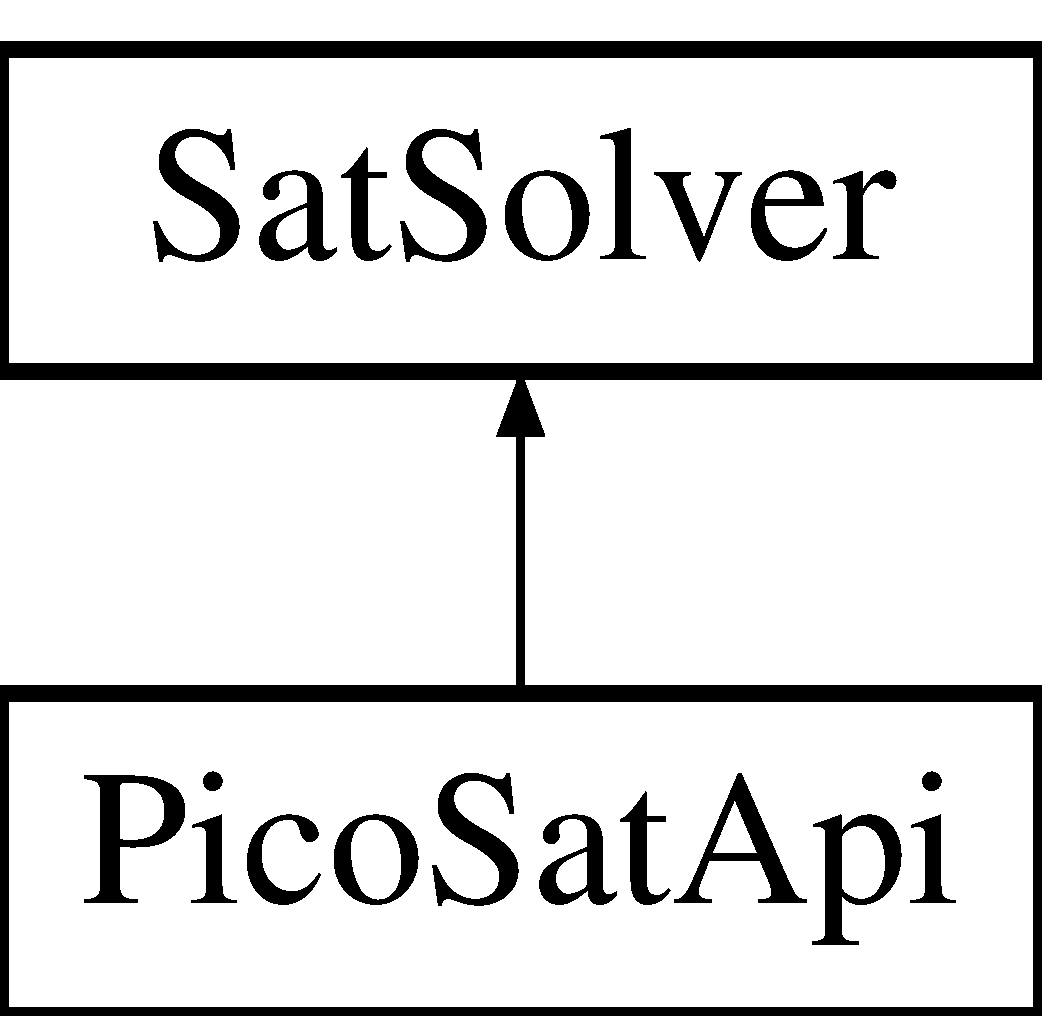
\includegraphics[height=2.000000cm]{classPicoSatApi}
\end{center}
\end{figure}
\subsection*{Public Member Functions}
\begin{DoxyCompactItemize}
\item 
\hyperlink{classPicoSatApi_a8d9525989ce86f149019a16a9ab665da}{Pico\-Sat\-Api} (bool rand\-\_\-models=false, bool min\-\_\-cores=true)
\begin{DoxyCompactList}\small\item\em Constructor. \end{DoxyCompactList}\item 
virtual \hyperlink{classPicoSatApi_aca9cd62b969f2d1dac2190962ecfb910}{$\sim$\-Pico\-Sat\-Api} ()
\begin{DoxyCompactList}\small\item\em Destructor. \end{DoxyCompactList}\item 
virtual bool \hyperlink{classPicoSatApi_a46ea721c61e298d87403476607ba9fe6}{is\-Sat} (const \hyperlink{classCNF}{C\-N\-F} \&cnf)
\begin{DoxyCompactList}\small\item\em Checks if a \hyperlink{classCNF}{C\-N\-F} is satisfiable. \end{DoxyCompactList}\item 
virtual bool \hyperlink{classPicoSatApi_a00dda1bd348d46bbfbf506f7735946da}{is\-Sat\-Model\-Or\-Core} (const \hyperlink{classCNF}{C\-N\-F} \&cnf, const vector$<$ int $>$ \&assumptions, const vector$<$ int $>$ \&vars\-\_\-of\-\_\-interest, vector$<$ int $>$ \&model\-\_\-or\-\_\-core)
\begin{DoxyCompactList}\small\item\em Checks if a \hyperlink{classCNF}{C\-N\-F} is satisfiable and extracts a model or an unsatisfiable core. \end{DoxyCompactList}\item 
virtual void \hyperlink{classPicoSatApi_a5e32634944d14142ab0e2c4fdeb12d85}{start\-Incremental\-Session} (const vector$<$ int $>$ \&vars\-\_\-to\-\_\-keep, bool use\-\_\-push=true)
\begin{DoxyCompactList}\small\item\em Starts a new incremental session. \end{DoxyCompactList}\item 
virtual void \hyperlink{classPicoSatApi_ae53598723725fd3203e2e32411392dab}{clear\-Incremental\-Session} ()
\begin{DoxyCompactList}\small\item\em Deletes the solver instance that is used in the incremental session. \end{DoxyCompactList}\item 
virtual void \hyperlink{classPicoSatApi_a619b3cb3b059b06c34f84d9ae123c042}{inc\-Add\-C\-N\-F} (const \hyperlink{classCNF}{C\-N\-F} \&cnf)
\begin{DoxyCompactList}\small\item\em Adds a new \hyperlink{classCNF}{C\-N\-F} to the current incremental session. \end{DoxyCompactList}\item 
virtual void \hyperlink{classPicoSatApi_aaafa1c5c7f1058029127a39a32ceada6}{inc\-Add\-Clause} (const vector$<$ int $>$ \&clause)
\begin{DoxyCompactList}\small\item\em Adds a new clause to the current incremental session. \end{DoxyCompactList}\item 
virtual void \hyperlink{classPicoSatApi_a0ef01830dacfd23f63928b44ff3df788}{inc\-Add\-Unit\-Clause} (int lit)
\begin{DoxyCompactList}\small\item\em Adds a new unit clause to the current incremental session. \end{DoxyCompactList}\item 
virtual void \hyperlink{classPicoSatApi_a5c31301a2b0dfc70251f285e737a6fc2}{inc\-Add2\-Lit\-Clause} (int lit1, int lit2)
\begin{DoxyCompactList}\small\item\em Adds a new clause consisting of 2 literals to the current incremental session. \end{DoxyCompactList}\item 
virtual void \hyperlink{classPicoSatApi_a1daeb6e2b3bfa3eee44a7bf1b278dd86}{inc\-Add3\-Lit\-Clause} (int lit1, int lit2, int lit3)
\begin{DoxyCompactList}\small\item\em Adds a new clause consisting of 3 literals to the current incremental session. \end{DoxyCompactList}\item 
virtual void \hyperlink{classPicoSatApi_ae0a7dd7da9ead164560f454e29457453}{inc\-Add\-Cube} (const vector$<$ int $>$ \&cube)
\begin{DoxyCompactList}\small\item\em Adds a new cube to the current incremental session. \end{DoxyCompactList}\item 
virtual void \hyperlink{classPicoSatApi_ace9bfbd0c8cbd62c3e92d2b208bb7b66}{inc\-Add\-Neg\-Cube\-As\-Clause} (const vector$<$ int $>$ \&cube)
\begin{DoxyCompactList}\small\item\em Adds the negation of a given cube (which is a clause) to the incremental session. \end{DoxyCompactList}\item 
virtual bool \hyperlink{classPicoSatApi_a0d1237c039315d572fb0828c59435177}{inc\-Is\-Sat} ()
\begin{DoxyCompactList}\small\item\em Checks if a the \hyperlink{classCNF}{C\-N\-F} in the incremental session is satisfiable. \end{DoxyCompactList}\item 
virtual bool \hyperlink{classPicoSatApi_abebe28c72303235d2fdc915bbf4752c0}{inc\-Is\-Sat} (const vector$<$ int $>$ \&assumptions)
\begin{DoxyCompactList}\small\item\em Checks if a the \hyperlink{classCNF}{C\-N\-F} in the incremental session is satisfiable under assumptions. \end{DoxyCompactList}\item 
virtual bool \hyperlink{classPicoSatApi_aa8c0dbf4587ff4666ce20fd325364c4a}{inc\-Is\-Sat\-Model\-Or\-Core} (const vector$<$ int $>$ \&assumptions, const vector$<$ int $>$ \&vars\-\_\-of\-\_\-interest, vector$<$ int $>$ \&model\-\_\-or\-\_\-core)
\begin{DoxyCompactList}\small\item\em Checks the \hyperlink{classCNF}{C\-N\-F} in the incremental session and computes a model or unsat core. \end{DoxyCompactList}\item 
virtual bool \hyperlink{classPicoSatApi_ada5b2d2ba3cf20b0ab007a62cc73028a}{inc\-Is\-Sat\-Model\-Or\-Core} (const vector$<$ int $>$ \&core\-\_\-assumptions, const vector$<$ int $>$ \&more\-\_\-assumptions, const vector$<$ int $>$ \&vars\-\_\-of\-\_\-interest, vector$<$ int $>$ \&model\-\_\-or\-\_\-core)
\begin{DoxyCompactList}\small\item\em Computes a satisfying assignment or core using additional assumptions. \end{DoxyCompactList}\item 
virtual void \hyperlink{classPicoSatApi_a523f9de3a59f927cb6ad0729e1caaac7}{inc\-Push} ()
\begin{DoxyCompactList}\small\item\em Stores the current state of the incremental session on a stack. \end{DoxyCompactList}\item 
virtual void \hyperlink{classPicoSatApi_a045c7a5229d4e45095922e1315c5c282}{inc\-Pop} ()
\begin{DoxyCompactList}\small\item\em Restores the incremental session back to the point where \hyperlink{classPicoSatApi_a523f9de3a59f927cb6ad0729e1caaac7}{inc\-Push()} was called. \end{DoxyCompactList}\item 
void \hyperlink{classSatSolver_a159fc9658709e5aeba2844a09454b2cb}{do\-Min\-Cores} (bool min\-\_\-cores=true)
\begin{DoxyCompactList}\small\item\em Enables or disables the computation of M\-I\-N\-I\-M\-A\-L unsatisfiable cores. \end{DoxyCompactList}\item 
void \hyperlink{classSatSolver_ae229c5e277350710412fce0e867dc566}{do\-Rand\-Models} (bool rand\-\_\-models=true)
\begin{DoxyCompactList}\small\item\em Enables or disables the randomization of satisfying assignments. \end{DoxyCompactList}\end{DoxyCompactItemize}
\subsection*{Protected Member Functions}
\begin{DoxyCompactItemize}
\item 
void \hyperlink{classPicoSatApi_ab0ded3e44578129ae266936de5e29a1c}{rand\-Model} (Pico\-S\-A\-T $\ast$solver, const vector$<$ int $>$ \&ass, vector$<$ int $>$ \&model)
\begin{DoxyCompactList}\small\item\em A helper to randomize a satisfying assignment after it has been computed. \end{DoxyCompactList}\end{DoxyCompactItemize}
\subsection*{Protected Attributes}
\begin{DoxyCompactItemize}
\item 
Pico\-S\-A\-T $\ast$ \hyperlink{classPicoSatApi_ae056afcfe07c468fd5b1488dc6f6e48d}{incr\-\_\-}
\begin{DoxyCompactList}\small\item\em The incremental solver instance. \end{DoxyCompactList}\item 
bool \hyperlink{classSatSolver_adfeecebfd09606c82b5c57cfe5aad813}{min\-\_\-cores\-\_\-}
\begin{DoxyCompactList}\small\item\em Indicates if the unsat cores returned by the solver should be minimized further. \end{DoxyCompactList}\item 
bool \hyperlink{classSatSolver_a73fed24d8fb4da85ef82dc53ac5f28c7}{rand\-\_\-models\-\_\-}
\begin{DoxyCompactList}\small\item\em Indicates if satisfying assignments should be randomized. \end{DoxyCompactList}\end{DoxyCompactItemize}
\subsection*{Private Member Functions}
\begin{DoxyCompactItemize}
\item 
\hyperlink{classPicoSatApi_a1d8cc76c346d85c8188db98793da93f9}{Pico\-Sat\-Api} (const \hyperlink{classPicoSatApi}{Pico\-Sat\-Api} \&other)
\begin{DoxyCompactList}\small\item\em Copy constructor. \end{DoxyCompactList}\item 
\hyperlink{classPicoSatApi}{Pico\-Sat\-Api} \& \hyperlink{classPicoSatApi_a17129e670ec8bb5d43f34c49a8b6ed87}{operator=} (const \hyperlink{classPicoSatApi}{Pico\-Sat\-Api} \&other)
\begin{DoxyCompactList}\small\item\em Assignment operator. \end{DoxyCompactList}\end{DoxyCompactItemize}


\subsection{Detailed Description}
Interfaces the Pico\-Sat S\-A\-T-\/solver via its A\-P\-I. 

This class represents an interface to the S\-A\-T-\/solver Pico\-Sat (see \href{http://fmv.jku.at/picosat/}{\tt http\-://fmv.\-jku.\-at/picosat/}). It is a concrete implementation of the \hyperlink{classSatSolver}{Sat\-Solver} interface. For a given \hyperlink{classCNF}{C\-N\-F}, this class is able to determine satisfiability. Furthermore, in case of satisfiability, it can extract satisfying assignments. In case of unsatisfiability, it can compute an unsatisfiable core. It can be used in two different ways. In the incremental usage scenario, all information the solver has learned so far is retained. Methods for incremental solving start with 'inc'. Other methods (like \hyperlink{classPicoSatApi_a46ea721c61e298d87403476607ba9fe6}{is\-Sat()} or \hyperlink{classPicoSatApi_a00dda1bd348d46bbfbf506f7735946da}{is\-Sat\-Model\-Or\-Core()}) instantiate a fresh solver instance for every call.

\begin{DoxyAuthor}{Author}
Robert Koenighofer (\href{mailto:robert.koenighofer@iaik.tugraz.at}{\tt robert.\-koenighofer@iaik.\-tugraz.\-at}) 
\end{DoxyAuthor}
\begin{DoxyVersion}{Version}
1.\-0.\-0 
\end{DoxyVersion}


Definition at line 55 of file Pico\-Sat\-Api.\-h.



\subsection{Constructor \& Destructor Documentation}
\hypertarget{classPicoSatApi_a8d9525989ce86f149019a16a9ab665da}{\index{Pico\-Sat\-Api@{Pico\-Sat\-Api}!Pico\-Sat\-Api@{Pico\-Sat\-Api}}
\index{Pico\-Sat\-Api@{Pico\-Sat\-Api}!PicoSatApi@{Pico\-Sat\-Api}}
\subsubsection[{Pico\-Sat\-Api}]{\setlength{\rightskip}{0pt plus 5cm}Pico\-Sat\-Api\-::\-Pico\-Sat\-Api (
\begin{DoxyParamCaption}
\item[{bool}]{rand\-\_\-models = {\ttfamily false}, }
\item[{bool}]{min\-\_\-cores = {\ttfamily true}}
\end{DoxyParamCaption}
)}}\label{classPicoSatApi_a8d9525989ce86f149019a16a9ab665da}


Constructor. 


\begin{DoxyParams}{Parameters}
{\em rand\-\_\-models} & A flag indicating if satisfying assignments should be randomized. This is done in a post-\/processing step (values are flipped randomly and then we check if this still constitutes a satisfying assignment). This is expensive. If this parameter is skipped, then satisfying assignments are not randomized. \\
\hline
{\em min\-\_\-cores} & A flag indicating if unsatisfiable cores returned by the solver should be minimized further by trying to drop one literal after the other. This makes the calls slower but produces potentially smaller cubes. \\
\hline
\end{DoxyParams}


Definition at line 38 of file Pico\-Sat\-Api.\-cpp.

\hypertarget{classPicoSatApi_aca9cd62b969f2d1dac2190962ecfb910}{\index{Pico\-Sat\-Api@{Pico\-Sat\-Api}!$\sim$\-Pico\-Sat\-Api@{$\sim$\-Pico\-Sat\-Api}}
\index{$\sim$\-Pico\-Sat\-Api@{$\sim$\-Pico\-Sat\-Api}!PicoSatApi@{Pico\-Sat\-Api}}
\subsubsection[{$\sim$\-Pico\-Sat\-Api}]{\setlength{\rightskip}{0pt plus 5cm}Pico\-Sat\-Api\-::$\sim$\-Pico\-Sat\-Api (
\begin{DoxyParamCaption}
{}
\end{DoxyParamCaption}
)\hspace{0.3cm}{\ttfamily [virtual]}}}\label{classPicoSatApi_aca9cd62b969f2d1dac2190962ecfb910}


Destructor. 



Definition at line 46 of file Pico\-Sat\-Api.\-cpp.



References clear\-Incremental\-Session().

\hypertarget{classPicoSatApi_a1d8cc76c346d85c8188db98793da93f9}{\index{Pico\-Sat\-Api@{Pico\-Sat\-Api}!Pico\-Sat\-Api@{Pico\-Sat\-Api}}
\index{Pico\-Sat\-Api@{Pico\-Sat\-Api}!PicoSatApi@{Pico\-Sat\-Api}}
\subsubsection[{Pico\-Sat\-Api}]{\setlength{\rightskip}{0pt plus 5cm}Pico\-Sat\-Api\-::\-Pico\-Sat\-Api (
\begin{DoxyParamCaption}
\item[{const {\bf Pico\-Sat\-Api} \&}]{other}
\end{DoxyParamCaption}
)\hspace{0.3cm}{\ttfamily [private]}}}\label{classPicoSatApi_a1d8cc76c346d85c8188db98793da93f9}


Copy constructor. 

The copy constructor is disabled (set private) and not implemented.


\begin{DoxyParams}{Parameters}
{\em other} & The source for creating the copy. \\
\hline
\end{DoxyParams}


\subsection{Member Function Documentation}
\hypertarget{classPicoSatApi_ae53598723725fd3203e2e32411392dab}{\index{Pico\-Sat\-Api@{Pico\-Sat\-Api}!clear\-Incremental\-Session@{clear\-Incremental\-Session}}
\index{clear\-Incremental\-Session@{clear\-Incremental\-Session}!PicoSatApi@{Pico\-Sat\-Api}}
\subsubsection[{clear\-Incremental\-Session}]{\setlength{\rightskip}{0pt plus 5cm}void Pico\-Sat\-Api\-::clear\-Incremental\-Session (
\begin{DoxyParamCaption}
{}
\end{DoxyParamCaption}
)\hspace{0.3cm}{\ttfamily [virtual]}}}\label{classPicoSatApi_ae53598723725fd3203e2e32411392dab}


Deletes the solver instance that is used in the incremental session. 



Implements \hyperlink{classSatSolver_a8118d2900f7acf31497cd2a27ad3b713}{Sat\-Solver}.



Definition at line 148 of file Pico\-Sat\-Api.\-cpp.



References incr\-\_\-.



Referenced by start\-Incremental\-Session(), and $\sim$\-Pico\-Sat\-Api().

\hypertarget{classSatSolver_a159fc9658709e5aeba2844a09454b2cb}{\index{Pico\-Sat\-Api@{Pico\-Sat\-Api}!do\-Min\-Cores@{do\-Min\-Cores}}
\index{do\-Min\-Cores@{do\-Min\-Cores}!PicoSatApi@{Pico\-Sat\-Api}}
\subsubsection[{do\-Min\-Cores}]{\setlength{\rightskip}{0pt plus 5cm}void Sat\-Solver\-::do\-Min\-Cores (
\begin{DoxyParamCaption}
\item[{bool}]{min\-\_\-cores = {\ttfamily true}}
\end{DoxyParamCaption}
)\hspace{0.3cm}{\ttfamily [inherited]}}}\label{classSatSolver_a159fc9658709e5aeba2844a09454b2cb}


Enables or disables the computation of M\-I\-N\-I\-M\-A\-L unsatisfiable cores. 


\begin{DoxyParams}{Parameters}
{\em min\-\_\-cores} & A flag indicating if unsatisfiable cores returned by the solver should be minimized further by trying to drop one literal after the other. This makes the calls slower but produces potentially smaller cubes. If the parameter is skipped the computation of minimal cores is enabled. \\
\hline
\end{DoxyParams}


Definition at line 47 of file Sat\-Solver.\-cpp.



References Sat\-Solver\-::min\-\_\-cores\-\_\-.



Referenced by Learn\-Synth\-S\-A\-T\-::compute\-Winning\-Region\-Plain(), Learn\-Synth\-S\-A\-T\-::compute\-Winning\-Region\-R\-G(), and Learn\-Synth\-S\-A\-T\-::compute\-Winning\-Region\-R\-G\-R\-C().

\hypertarget{classSatSolver_ae229c5e277350710412fce0e867dc566}{\index{Pico\-Sat\-Api@{Pico\-Sat\-Api}!do\-Rand\-Models@{do\-Rand\-Models}}
\index{do\-Rand\-Models@{do\-Rand\-Models}!PicoSatApi@{Pico\-Sat\-Api}}
\subsubsection[{do\-Rand\-Models}]{\setlength{\rightskip}{0pt plus 5cm}void Sat\-Solver\-::do\-Rand\-Models (
\begin{DoxyParamCaption}
\item[{bool}]{rand\-\_\-models = {\ttfamily true}}
\end{DoxyParamCaption}
)\hspace{0.3cm}{\ttfamily [inherited]}}}\label{classSatSolver_ae229c5e277350710412fce0e867dc566}


Enables or disables the randomization of satisfying assignments. 


\begin{DoxyParams}{Parameters}
{\em rand\-\_\-models} & A flag indicating if satisfying assignments should be randomized. This is done in a post-\/processing step (values are flipped randomly and then we check if this still constitutes a satisfying assignment). This is expensive. If this parameter is skipped, then randomization is enabled. \\
\hline
\end{DoxyParams}


Definition at line 53 of file Sat\-Solver.\-cpp.



References Sat\-Solver\-::rand\-\_\-models\-\_\-.



Referenced by Learn\-Synth\-S\-A\-T\-::compute\-Winning\-Region\-Plain(), Learn\-Synth\-S\-A\-T\-::compute\-Winning\-Region\-R\-G(), and Learn\-Synth\-S\-A\-T\-::compute\-Winning\-Region\-R\-G\-R\-C().

\hypertarget{classPicoSatApi_a5c31301a2b0dfc70251f285e737a6fc2}{\index{Pico\-Sat\-Api@{Pico\-Sat\-Api}!inc\-Add2\-Lit\-Clause@{inc\-Add2\-Lit\-Clause}}
\index{inc\-Add2\-Lit\-Clause@{inc\-Add2\-Lit\-Clause}!PicoSatApi@{Pico\-Sat\-Api}}
\subsubsection[{inc\-Add2\-Lit\-Clause}]{\setlength{\rightskip}{0pt plus 5cm}void Pico\-Sat\-Api\-::inc\-Add2\-Lit\-Clause (
\begin{DoxyParamCaption}
\item[{int}]{lit1, }
\item[{int}]{lit2}
\end{DoxyParamCaption}
)\hspace{0.3cm}{\ttfamily [virtual]}}}\label{classPicoSatApi_a5c31301a2b0dfc70251f285e737a6fc2}


Adds a new clause consisting of 2 literals to the current incremental session. 

\begin{DoxyPrecond}{Precondition}
\hyperlink{classPicoSatApi_a5e32634944d14142ab0e2c4fdeb12d85}{start\-Incremental\-Session()} must have been called before. 
\end{DoxyPrecond}

\begin{DoxyParams}{Parameters}
{\em lit1} & The first literal of the clause to add to the currently open incremental session. If this method is called after solving for the first time, be sure that the passed literal talks about a variables that have been mentioned in vars\-\_\-to\-\_\-keep when calling \hyperlink{classPicoSatApi_a5e32634944d14142ab0e2c4fdeb12d85}{start\-Incremental\-Session()}. Actually, the implementation in T\-H\-I\-S class does not care, but other implementations of the \hyperlink{classSatSolver}{Sat\-Solver} interface do. Hence, you should not violate this property to have the solver instances exchangeable. \\
\hline
{\em lit2} & The second literal of the clause to add to the currently open incremental session (must be contained in vars\-\_\-to\-\_\-keep as well). \\
\hline
\end{DoxyParams}


Implements \hyperlink{classSatSolver_a791be541b59ef58a29a1c517fca943e7}{Sat\-Solver}.



Definition at line 188 of file Pico\-Sat\-Api.\-cpp.



References incr\-\_\-, and M\-A\-S\-S\-E\-R\-T.

\hypertarget{classPicoSatApi_a1daeb6e2b3bfa3eee44a7bf1b278dd86}{\index{Pico\-Sat\-Api@{Pico\-Sat\-Api}!inc\-Add3\-Lit\-Clause@{inc\-Add3\-Lit\-Clause}}
\index{inc\-Add3\-Lit\-Clause@{inc\-Add3\-Lit\-Clause}!PicoSatApi@{Pico\-Sat\-Api}}
\subsubsection[{inc\-Add3\-Lit\-Clause}]{\setlength{\rightskip}{0pt plus 5cm}void Pico\-Sat\-Api\-::inc\-Add3\-Lit\-Clause (
\begin{DoxyParamCaption}
\item[{int}]{lit1, }
\item[{int}]{lit2, }
\item[{int}]{lit3}
\end{DoxyParamCaption}
)\hspace{0.3cm}{\ttfamily [virtual]}}}\label{classPicoSatApi_a1daeb6e2b3bfa3eee44a7bf1b278dd86}


Adds a new clause consisting of 3 literals to the current incremental session. 

\begin{DoxyPrecond}{Precondition}
\hyperlink{classPicoSatApi_a5e32634944d14142ab0e2c4fdeb12d85}{start\-Incremental\-Session()} must have been called before. 
\end{DoxyPrecond}

\begin{DoxyParams}{Parameters}
{\em lit1} & The first literal of the clause to add to the currently open incremental session. If this method is called after solving for the first time, be sure that the passed literal talks about a variables that have been mentioned in vars\-\_\-to\-\_\-keep when calling \hyperlink{classPicoSatApi_a5e32634944d14142ab0e2c4fdeb12d85}{start\-Incremental\-Session()}. Actually, the implementation in T\-H\-I\-S class does not care, but other implementations of the \hyperlink{classSatSolver}{Sat\-Solver} interface do. Hence, you should not violate this property to have the solver instances exchangeable. \\
\hline
{\em lit2} & The second literal of the clause to add to the currently open incremental session (must be contained in vars\-\_\-to\-\_\-keep as well). \\
\hline
{\em lit3} & The third literal of the clause to add to the currently open incremental session (must be contained in vars\-\_\-to\-\_\-keep as well). \\
\hline
\end{DoxyParams}


Implements \hyperlink{classSatSolver_abca288874a1b8ab1a90cb274eb885ace}{Sat\-Solver}.



Definition at line 197 of file Pico\-Sat\-Api.\-cpp.



References incr\-\_\-, and M\-A\-S\-S\-E\-R\-T.

\hypertarget{classPicoSatApi_aaafa1c5c7f1058029127a39a32ceada6}{\index{Pico\-Sat\-Api@{Pico\-Sat\-Api}!inc\-Add\-Clause@{inc\-Add\-Clause}}
\index{inc\-Add\-Clause@{inc\-Add\-Clause}!PicoSatApi@{Pico\-Sat\-Api}}
\subsubsection[{inc\-Add\-Clause}]{\setlength{\rightskip}{0pt plus 5cm}void Pico\-Sat\-Api\-::inc\-Add\-Clause (
\begin{DoxyParamCaption}
\item[{const vector$<$ int $>$ \&}]{clause}
\end{DoxyParamCaption}
)\hspace{0.3cm}{\ttfamily [virtual]}}}\label{classPicoSatApi_aaafa1c5c7f1058029127a39a32ceada6}


Adds a new clause to the current incremental session. 

\begin{DoxyPrecond}{Precondition}
\hyperlink{classPicoSatApi_a5e32634944d14142ab0e2c4fdeb12d85}{start\-Incremental\-Session()} must have been called before. 
\end{DoxyPrecond}

\begin{DoxyParams}{Parameters}
{\em clause} & The clause (a disjunction of literals) to add (conjunct) to the currently open incremental session. If this method is called after solving for the first time, be sure that the passed clause talks only about variables that have been mentioned in vars\-\_\-to\-\_\-keep when calling \hyperlink{classPicoSatApi_a5e32634944d14142ab0e2c4fdeb12d85}{start\-Incremental\-Session()}. Actually, the implementation in T\-H\-I\-S class does not care, but other implementations of the \hyperlink{classSatSolver}{Sat\-Solver} interface do. Hence, you should not violate this property to have the solver instances exchangeable. \\
\hline
\end{DoxyParams}


Implements \hyperlink{classSatSolver_a9f91c104238b6e091513e0aa46970840}{Sat\-Solver}.



Definition at line 171 of file Pico\-Sat\-Api.\-cpp.



References incr\-\_\-, and M\-A\-S\-S\-E\-R\-T.

\hypertarget{classPicoSatApi_a619b3cb3b059b06c34f84d9ae123c042}{\index{Pico\-Sat\-Api@{Pico\-Sat\-Api}!inc\-Add\-C\-N\-F@{inc\-Add\-C\-N\-F}}
\index{inc\-Add\-C\-N\-F@{inc\-Add\-C\-N\-F}!PicoSatApi@{Pico\-Sat\-Api}}
\subsubsection[{inc\-Add\-C\-N\-F}]{\setlength{\rightskip}{0pt plus 5cm}void Pico\-Sat\-Api\-::inc\-Add\-C\-N\-F (
\begin{DoxyParamCaption}
\item[{const {\bf C\-N\-F} \&}]{cnf}
\end{DoxyParamCaption}
)\hspace{0.3cm}{\ttfamily [virtual]}}}\label{classPicoSatApi_a619b3cb3b059b06c34f84d9ae123c042}


Adds a new \hyperlink{classCNF}{C\-N\-F} to the current incremental session. 

\begin{DoxyPrecond}{Precondition}
\hyperlink{classPicoSatApi_a5e32634944d14142ab0e2c4fdeb12d85}{start\-Incremental\-Session()} must have been called before. 
\end{DoxyPrecond}

\begin{DoxyParams}{Parameters}
{\em cnf} & The \hyperlink{classCNF}{C\-N\-F} to add to the currently open incremental session. If this method is called after solving for the first time, be sure that the passed \hyperlink{classCNF}{C\-N\-F} talks only about variables that have been mentioned in vars\-\_\-to\-\_\-keep when calling \hyperlink{classPicoSatApi_a5e32634944d14142ab0e2c4fdeb12d85}{start\-Incremental\-Session()}. Actually, the implementation in T\-H\-I\-S class does not care, but other implementations of the \hyperlink{classSatSolver}{Sat\-Solver} interface do. Hence, you should not violate this property to have the solver instances exchangeable. \\
\hline
\end{DoxyParams}


Implements \hyperlink{classSatSolver_ab2581b192cb2c39a81a416a9f7416c9e}{Sat\-Solver}.



Definition at line 158 of file Pico\-Sat\-Api.\-cpp.



References C\-N\-F\-::get\-Clauses(), incr\-\_\-, and M\-A\-S\-S\-E\-R\-T.

\hypertarget{classPicoSatApi_ae0a7dd7da9ead164560f454e29457453}{\index{Pico\-Sat\-Api@{Pico\-Sat\-Api}!inc\-Add\-Cube@{inc\-Add\-Cube}}
\index{inc\-Add\-Cube@{inc\-Add\-Cube}!PicoSatApi@{Pico\-Sat\-Api}}
\subsubsection[{inc\-Add\-Cube}]{\setlength{\rightskip}{0pt plus 5cm}void Pico\-Sat\-Api\-::inc\-Add\-Cube (
\begin{DoxyParamCaption}
\item[{const vector$<$ int $>$ \&}]{cube}
\end{DoxyParamCaption}
)\hspace{0.3cm}{\ttfamily [virtual]}}}\label{classPicoSatApi_ae0a7dd7da9ead164560f454e29457453}


Adds a new cube to the current incremental session. 

That is, all literals of the cube are added as unit clauses to the current incremental session. For instance, if the cube \mbox{[}2, -\/4, 8\mbox{]} is passed as argument, then this method adds the three unit clauses \mbox{[}2\mbox{]}, \mbox{[}-\/4\mbox{]}, \mbox{[}8\mbox{]}.

\begin{DoxyPrecond}{Precondition}
\hyperlink{classPicoSatApi_a5e32634944d14142ab0e2c4fdeb12d85}{start\-Incremental\-Session()} must have been called before. 
\end{DoxyPrecond}

\begin{DoxyParams}{Parameters}
{\em cube} & The cube (a conjunction of literals) to add (conjunct) to the currently open incremental session. All literals of this cube will be added as unit clauses. If this method is called after solving for the first time, be sure that the passed clause talks only about variables that have been mentioned in vars\-\_\-to\-\_\-keep when calling \hyperlink{classPicoSatApi_a5e32634944d14142ab0e2c4fdeb12d85}{start\-Incremental\-Session()}. Actually, the implementation in T\-H\-I\-S class does not care, but other implementations of the \hyperlink{classSatSolver}{Sat\-Solver} interface do. Hence, you should not violate this property to have the solver instances exchangeable. \\
\hline
\end{DoxyParams}


Implements \hyperlink{classSatSolver_a1f04f34bb04174489ed18d0b62241004}{Sat\-Solver}.



Definition at line 207 of file Pico\-Sat\-Api.\-cpp.



References incr\-\_\-, and M\-A\-S\-S\-E\-R\-T.

\hypertarget{classPicoSatApi_ace9bfbd0c8cbd62c3e92d2b208bb7b66}{\index{Pico\-Sat\-Api@{Pico\-Sat\-Api}!inc\-Add\-Neg\-Cube\-As\-Clause@{inc\-Add\-Neg\-Cube\-As\-Clause}}
\index{inc\-Add\-Neg\-Cube\-As\-Clause@{inc\-Add\-Neg\-Cube\-As\-Clause}!PicoSatApi@{Pico\-Sat\-Api}}
\subsubsection[{inc\-Add\-Neg\-Cube\-As\-Clause}]{\setlength{\rightskip}{0pt plus 5cm}void Pico\-Sat\-Api\-::inc\-Add\-Neg\-Cube\-As\-Clause (
\begin{DoxyParamCaption}
\item[{const vector$<$ int $>$ \&}]{cube}
\end{DoxyParamCaption}
)\hspace{0.3cm}{\ttfamily [virtual]}}}\label{classPicoSatApi_ace9bfbd0c8cbd62c3e92d2b208bb7b66}


Adds the negation of a given cube (which is a clause) to the incremental session. 

For instance, if the cube \mbox{[}2, -\/4, 8\mbox{]} is passed as argument, then this method adds the clauses \mbox{[}-\/2, 4, -\/8\mbox{]} to the current incremental session.

\begin{DoxyPrecond}{Precondition}
\hyperlink{classPicoSatApi_a5e32634944d14142ab0e2c4fdeb12d85}{start\-Incremental\-Session()} must have been called before. 
\end{DoxyPrecond}

\begin{DoxyParams}{Parameters}
{\em cube} & The cube (a conjunction of literals) to negate and add (conjunct) to the currently open incremental session. If this method is called after solving for the first time, be sure that the passed cube talks only about variables that have been mentioned in vars\-\_\-to\-\_\-keep when calling \hyperlink{classPicoSatApi_a5e32634944d14142ab0e2c4fdeb12d85}{start\-Incremental\-Session()}. Actually, the implementation in T\-H\-I\-S class does not care, but other implementations of the \hyperlink{classSatSolver}{Sat\-Solver} interface do. Hence, you should not violate this property to have the solver instances exchangeable. \\
\hline
\end{DoxyParams}


Implements \hyperlink{classSatSolver_a6be2c564289a59057c4c6728a3aa9c2b}{Sat\-Solver}.



Definition at line 218 of file Pico\-Sat\-Api.\-cpp.



References incr\-\_\-, and M\-A\-S\-S\-E\-R\-T.

\hypertarget{classPicoSatApi_a0ef01830dacfd23f63928b44ff3df788}{\index{Pico\-Sat\-Api@{Pico\-Sat\-Api}!inc\-Add\-Unit\-Clause@{inc\-Add\-Unit\-Clause}}
\index{inc\-Add\-Unit\-Clause@{inc\-Add\-Unit\-Clause}!PicoSatApi@{Pico\-Sat\-Api}}
\subsubsection[{inc\-Add\-Unit\-Clause}]{\setlength{\rightskip}{0pt plus 5cm}void Pico\-Sat\-Api\-::inc\-Add\-Unit\-Clause (
\begin{DoxyParamCaption}
\item[{int}]{lit}
\end{DoxyParamCaption}
)\hspace{0.3cm}{\ttfamily [virtual]}}}\label{classPicoSatApi_a0ef01830dacfd23f63928b44ff3df788}


Adds a new unit clause to the current incremental session. 

\begin{DoxyPrecond}{Precondition}
\hyperlink{classPicoSatApi_a5e32634944d14142ab0e2c4fdeb12d85}{start\-Incremental\-Session()} must have been called before. 
\end{DoxyPrecond}

\begin{DoxyParams}{Parameters}
{\em lit} & The (one and only) literal of the unit clause to add to the currently open incremental session. If this method is called after solving for the first time, be sure that the passed literal talks about a variables that have been mentioned in vars\-\_\-to\-\_\-keep when calling \hyperlink{classPicoSatApi_a5e32634944d14142ab0e2c4fdeb12d85}{start\-Incremental\-Session()}. Actually, the implementation in T\-H\-I\-S class does not care, but other implementations of the \hyperlink{classSatSolver}{Sat\-Solver} interface do. Hence, you should not violate this property to have the solver instances exchangeable. \\
\hline
\end{DoxyParams}


Implements \hyperlink{classSatSolver_a5b39c45cd2a1abfe96c681515dfddb77}{Sat\-Solver}.



Definition at line 180 of file Pico\-Sat\-Api.\-cpp.



References incr\-\_\-, and M\-A\-S\-S\-E\-R\-T.

\hypertarget{classPicoSatApi_a0d1237c039315d572fb0828c59435177}{\index{Pico\-Sat\-Api@{Pico\-Sat\-Api}!inc\-Is\-Sat@{inc\-Is\-Sat}}
\index{inc\-Is\-Sat@{inc\-Is\-Sat}!PicoSatApi@{Pico\-Sat\-Api}}
\subsubsection[{inc\-Is\-Sat}]{\setlength{\rightskip}{0pt plus 5cm}bool Pico\-Sat\-Api\-::inc\-Is\-Sat (
\begin{DoxyParamCaption}
{}
\end{DoxyParamCaption}
)\hspace{0.3cm}{\ttfamily [virtual]}}}\label{classPicoSatApi_a0d1237c039315d572fb0828c59435177}


Checks if a the \hyperlink{classCNF}{C\-N\-F} in the incremental session is satisfiable. 

\begin{DoxyPrecond}{Precondition}
\hyperlink{classPicoSatApi_a5e32634944d14142ab0e2c4fdeb12d85}{start\-Incremental\-Session()} must have been called before. 
\end{DoxyPrecond}
\begin{DoxyReturn}{Returns}
True in case of satisfiability, false otherwise. 
\end{DoxyReturn}


Implements \hyperlink{classSatSolver_ab1aab4b96a36b2003450067a3799ae23}{Sat\-Solver}.



Definition at line 227 of file Pico\-Sat\-Api.\-cpp.



References incr\-\_\-, and M\-A\-S\-S\-E\-R\-T.

\hypertarget{classPicoSatApi_abebe28c72303235d2fdc915bbf4752c0}{\index{Pico\-Sat\-Api@{Pico\-Sat\-Api}!inc\-Is\-Sat@{inc\-Is\-Sat}}
\index{inc\-Is\-Sat@{inc\-Is\-Sat}!PicoSatApi@{Pico\-Sat\-Api}}
\subsubsection[{inc\-Is\-Sat}]{\setlength{\rightskip}{0pt plus 5cm}bool Pico\-Sat\-Api\-::inc\-Is\-Sat (
\begin{DoxyParamCaption}
\item[{const vector$<$ int $>$ \&}]{assumptions}
\end{DoxyParamCaption}
)\hspace{0.3cm}{\ttfamily [virtual]}}}\label{classPicoSatApi_abebe28c72303235d2fdc915bbf4752c0}


Checks if a the \hyperlink{classCNF}{C\-N\-F} in the incremental session is satisfiable under assumptions. 

This method checks if the \hyperlink{classCNF}{C\-N\-F} in the incremental session is satisfiable given that all literals passed in the vector 'assumptions' are true. The assumptions are not persistently added to the \hyperlink{classCNF}{C\-N\-F} of the incremental session.

\begin{DoxyPrecond}{Precondition}
\hyperlink{classPicoSatApi_a5e32634944d14142ab0e2c4fdeb12d85}{start\-Incremental\-Session()} must have been called before. 
\end{DoxyPrecond}

\begin{DoxyParams}{Parameters}
{\em assumptions} & A vector of literals. This method then checks if the \hyperlink{classCNF}{C\-N\-F} of the incremental session is satisfiable given that all literals passed in this vector are true. The assumptions are not persistently added to the \hyperlink{classCNF}{C\-N\-F}. The assumptions must be a subset of the vars\-\_\-to\-\_\-keep passed to \hyperlink{classPicoSatApi_a5e32634944d14142ab0e2c4fdeb12d85}{start\-Incremental\-Session()}. \\
\hline
\end{DoxyParams}
\begin{DoxyReturn}{Returns}
True in case of satisfiability, false otherwise. 
\end{DoxyReturn}


Implements \hyperlink{classSatSolver_a1864787a33621efac7fc75fb6b25f080}{Sat\-Solver}.



Definition at line 240 of file Pico\-Sat\-Api.\-cpp.



References incr\-\_\-, and M\-A\-S\-S\-E\-R\-T.

\hypertarget{classPicoSatApi_aa8c0dbf4587ff4666ce20fd325364c4a}{\index{Pico\-Sat\-Api@{Pico\-Sat\-Api}!inc\-Is\-Sat\-Model\-Or\-Core@{inc\-Is\-Sat\-Model\-Or\-Core}}
\index{inc\-Is\-Sat\-Model\-Or\-Core@{inc\-Is\-Sat\-Model\-Or\-Core}!PicoSatApi@{Pico\-Sat\-Api}}
\subsubsection[{inc\-Is\-Sat\-Model\-Or\-Core}]{\setlength{\rightskip}{0pt plus 5cm}bool Pico\-Sat\-Api\-::inc\-Is\-Sat\-Model\-Or\-Core (
\begin{DoxyParamCaption}
\item[{const vector$<$ int $>$ \&}]{assumptions, }
\item[{const vector$<$ int $>$ \&}]{vars\-\_\-of\-\_\-interest, }
\item[{vector$<$ int $>$ \&}]{model\-\_\-or\-\_\-core}
\end{DoxyParamCaption}
)\hspace{0.3cm}{\ttfamily [virtual]}}}\label{classPicoSatApi_aa8c0dbf4587ff4666ce20fd325364c4a}


Checks the \hyperlink{classCNF}{C\-N\-F} in the incremental session and computes a model or unsat core. 

This method checks if the \hyperlink{classCNF}{C\-N\-F} of the incremental session is satisfiable given that all literals passed in the vector 'assumptions' is true. If this is the case, then a satisfying assignment will be written into model\-\_\-or\-\_\-core. You can specify which variables you want to have in the satisfying assignment using the vars\-\_\-of\-\_\-interest vector. The reason is that your \hyperlink{classCNF}{C\-N\-F} may contain thousands of temporary variables stemming from some Tseitin encoding, but usually one in only interested in the value of a few variables. In case of unsatisfiability, an unsatisfiable core is stored in model\-\_\-or\-\_\-core. The unsatisfiable core is a subset of the literals passed in 'assumptions' such that the \hyperlink{classCNF}{C\-N\-F} is still unsatisfiable when these literals hold.


\begin{DoxyParams}{Parameters}
{\em assumptions} & A vector of literals. This method then checks if the \hyperlink{classCNF}{C\-N\-F} of the incremental session is satisfiable given that all literals passed in this vector are true. The assumptions are not persistently added to the \hyperlink{classCNF}{C\-N\-F}. The assumptions must be a subset of the vars\-\_\-to\-\_\-keep passed to \hyperlink{classPicoSatApi_a5e32634944d14142ab0e2c4fdeb12d85}{start\-Incremental\-Session()}. \\
\hline
{\em vars\-\_\-of\-\_\-interest} & The variables for which you want to have a value in case of satisfiability. vars\-\_\-of\-\_\-interest must be a subset of the vars\-\_\-to\-\_\-keep passed to \hyperlink{classPicoSatApi_a5e32634944d14142ab0e2c4fdeb12d85}{start\-Incremental\-Session()}. \\
\hline
{\em model\-\_\-or\-\_\-core} & An empty vector. Depending on the outcome of the call, either a satisfying assignment (a cube over the variables passed in vars\-\_\-of\-\_\-interest) or an unsatisfiable core (a subset of the literals passed in 'assumptions') will be written into this vector. \\
\hline
\end{DoxyParams}
\begin{DoxyReturn}{Returns}
True in case of satisfiability (of the \hyperlink{classCNF}{C\-N\-F} of the incremental session in conjunction conjuncted with all assumptions), false otherwise. 
\end{DoxyReturn}


Implements \hyperlink{classSatSolver_ad387fc06bacf2d48847f779c9db8461a}{Sat\-Solver}.



Definition at line 255 of file Pico\-Sat\-Api.\-cpp.



References incr\-\_\-, M\-A\-S\-S\-E\-R\-T, Sat\-Solver\-::min\-\_\-cores\-\_\-, Sat\-Solver\-::rand\-\_\-models\-\_\-, rand\-Model(), and Utils\-::remove().

\hypertarget{classPicoSatApi_ada5b2d2ba3cf20b0ab007a62cc73028a}{\index{Pico\-Sat\-Api@{Pico\-Sat\-Api}!inc\-Is\-Sat\-Model\-Or\-Core@{inc\-Is\-Sat\-Model\-Or\-Core}}
\index{inc\-Is\-Sat\-Model\-Or\-Core@{inc\-Is\-Sat\-Model\-Or\-Core}!PicoSatApi@{Pico\-Sat\-Api}}
\subsubsection[{inc\-Is\-Sat\-Model\-Or\-Core}]{\setlength{\rightskip}{0pt plus 5cm}bool Pico\-Sat\-Api\-::inc\-Is\-Sat\-Model\-Or\-Core (
\begin{DoxyParamCaption}
\item[{const vector$<$ int $>$ \&}]{core\-\_\-assumptions, }
\item[{const vector$<$ int $>$ \&}]{more\-\_\-assumptions, }
\item[{const vector$<$ int $>$ \&}]{vars\-\_\-of\-\_\-interest, }
\item[{vector$<$ int $>$ \&}]{model\-\_\-or\-\_\-core}
\end{DoxyParamCaption}
)\hspace{0.3cm}{\ttfamily [virtual]}}}\label{classPicoSatApi_ada5b2d2ba3cf20b0ab007a62cc73028a}


Computes a satisfying assignment or core using additional assumptions. 

In contrast to the previous method, this one allows to define two sets of assumptions. The core\-\_\-assumptions are used as basis for extracting an unsatisfiable core in case of unsatisfiability. The more\-\_\-assumptions are assumed but not considered for the computation of unsatisfiable cores. This is convenient to avoid calls to \hyperlink{classPicoSatApi_a523f9de3a59f927cb6ad0729e1caaac7}{inc\-Push()} and \hyperlink{classPicoSatApi_a045c7a5229d4e45095922e1315c5c282}{inc\-Pop()} when temporarily working under assumptions that should not be minimized for the unsatisfiable core.


\begin{DoxyParams}{Parameters}
{\em core\-\_\-assumptions} & A vector of literals. This method then checks if the \hyperlink{classCNF}{C\-N\-F} of the incremental session is satisfiable given that all literals passed in this vector and all literals passed in more\-\_\-assumptions are true. However, for computing the the unsatisfiable core, only the core\-\_\-assumptions will be minimized and the more\-\_\-assumptions stay as they are. That is, in case of unsatisfiability, model\-\_\-or\-\_\-core will contain a subset X of the core\-\_\-assumptions such that X \& more\-\_\-assumptions \& incremental\-\_\-cnf is still unsatisfiable. core\-\_\-assumptions must be a subset of the vars\-\_\-to\-\_\-keep passed to \hyperlink{classPicoSatApi_a5e32634944d14142ab0e2c4fdeb12d85}{start\-Incremental\-Session()}. \\
\hline
{\em more\-\_\-assumptions} & A vector of assumptions that are assumed, but not minimized when an unsatisfiable core is computed. That is, in case of unsatisfiability, model\-\_\-or\-\_\-core will contain a subset X of the core\-\_\-assumptions such that X \& more\-\_\-assumptions \& incremental\-\_\-cnf is still unsatisfiable. more\-\_\-assumptions must be a subset of the vars\-\_\-to\-\_\-keep passed to \hyperlink{classPicoSatApi_a5e32634944d14142ab0e2c4fdeb12d85}{start\-Incremental\-Session()}. \\
\hline
{\em vars\-\_\-of\-\_\-interest} & The variables for which you want to have a value in case of satisfiability. vars\-\_\-of\-\_\-interest must be a subset of the vars\-\_\-to\-\_\-keep passed to \hyperlink{classPicoSatApi_a5e32634944d14142ab0e2c4fdeb12d85}{start\-Incremental\-Session()}. \\
\hline
{\em model\-\_\-or\-\_\-core} & An empty vector. Depending on the outcome of the call, either a satisfying assignment (a cube over the variables passed in vars\-\_\-of\-\_\-interest) or an unsatisfiable core (a subset of the literals passed in 'core\-\_\-assumptions') will be written into this vector. \\
\hline
\end{DoxyParams}
\begin{DoxyReturn}{Returns}
True in case of satisfiability (of the \hyperlink{classCNF}{C\-N\-F} of the incremental session in conjunction conjuncted with all assumptions), false otherwise. 
\end{DoxyReturn}


Implements \hyperlink{classSatSolver_a29225bfab1f352cae27c68e9bda4d409}{Sat\-Solver}.



Definition at line 319 of file Pico\-Sat\-Api.\-cpp.



References incr\-\_\-, M\-A\-S\-S\-E\-R\-T, Sat\-Solver\-::min\-\_\-cores\-\_\-, Sat\-Solver\-::rand\-\_\-models\-\_\-, rand\-Model(), and Utils\-::remove().

\hypertarget{classPicoSatApi_a045c7a5229d4e45095922e1315c5c282}{\index{Pico\-Sat\-Api@{Pico\-Sat\-Api}!inc\-Pop@{inc\-Pop}}
\index{inc\-Pop@{inc\-Pop}!PicoSatApi@{Pico\-Sat\-Api}}
\subsubsection[{inc\-Pop}]{\setlength{\rightskip}{0pt plus 5cm}void Pico\-Sat\-Api\-::inc\-Pop (
\begin{DoxyParamCaption}
{}
\end{DoxyParamCaption}
)\hspace{0.3cm}{\ttfamily [virtual]}}}\label{classPicoSatApi_a045c7a5229d4e45095922e1315c5c282}


Restores the incremental session back to the point where \hyperlink{classPicoSatApi_a523f9de3a59f927cb6ad0729e1caaac7}{inc\-Push()} was called. 



Implements \hyperlink{classSatSolver_a436aae045eb04141c834df0b55947ee5}{Sat\-Solver}.



Definition at line 401 of file Pico\-Sat\-Api.\-cpp.



References incr\-\_\-, and M\-A\-S\-S\-E\-R\-T.

\hypertarget{classPicoSatApi_a523f9de3a59f927cb6ad0729e1caaac7}{\index{Pico\-Sat\-Api@{Pico\-Sat\-Api}!inc\-Push@{inc\-Push}}
\index{inc\-Push@{inc\-Push}!PicoSatApi@{Pico\-Sat\-Api}}
\subsubsection[{inc\-Push}]{\setlength{\rightskip}{0pt plus 5cm}void Pico\-Sat\-Api\-::inc\-Push (
\begin{DoxyParamCaption}
{}
\end{DoxyParamCaption}
)\hspace{0.3cm}{\ttfamily [virtual]}}}\label{classPicoSatApi_a523f9de3a59f927cb6ad0729e1caaac7}


Stores the current state of the incremental session on a stack. 

The state can be restored later by calling \hyperlink{classPicoSatApi_a045c7a5229d4e45095922e1315c5c282}{inc\-Pop()}. 

Implements \hyperlink{classSatSolver_a4da0dff7082a91429e3311d279605be4}{Sat\-Solver}.



Definition at line 394 of file Pico\-Sat\-Api.\-cpp.



References incr\-\_\-, and M\-A\-S\-S\-E\-R\-T.

\hypertarget{classPicoSatApi_a46ea721c61e298d87403476607ba9fe6}{\index{Pico\-Sat\-Api@{Pico\-Sat\-Api}!is\-Sat@{is\-Sat}}
\index{is\-Sat@{is\-Sat}!PicoSatApi@{Pico\-Sat\-Api}}
\subsubsection[{is\-Sat}]{\setlength{\rightskip}{0pt plus 5cm}bool Pico\-Sat\-Api\-::is\-Sat (
\begin{DoxyParamCaption}
\item[{const {\bf C\-N\-F} \&}]{cnf}
\end{DoxyParamCaption}
)\hspace{0.3cm}{\ttfamily [virtual]}}}\label{classPicoSatApi_a46ea721c61e298d87403476607ba9fe6}


Checks if a \hyperlink{classCNF}{C\-N\-F} is satisfiable. 

This method is not incremental. At aver call to this method, a new solver instance is created and deleted afterwards. This method does not interfere with an incremental session that may be open in parallel.


\begin{DoxyParams}{Parameters}
{\em cnf} & The \hyperlink{classCNF}{C\-N\-F} formula for which we want to know if it is satisfiable. \\
\hline
\end{DoxyParams}
\begin{DoxyReturn}{Returns}
True in case of satisfiability, false otherwise. 
\end{DoxyReturn}


Implements \hyperlink{classSatSolver_a82f60f60db464fbe5c66a20ad673a573}{Sat\-Solver}.



Definition at line 52 of file Pico\-Sat\-Api.\-cpp.



References C\-N\-F\-::get\-Clauses(), and M\-A\-S\-S\-E\-R\-T.



Referenced by is\-Sat\-Model\-Or\-Core().

\hypertarget{classPicoSatApi_a00dda1bd348d46bbfbf506f7735946da}{\index{Pico\-Sat\-Api@{Pico\-Sat\-Api}!is\-Sat\-Model\-Or\-Core@{is\-Sat\-Model\-Or\-Core}}
\index{is\-Sat\-Model\-Or\-Core@{is\-Sat\-Model\-Or\-Core}!PicoSatApi@{Pico\-Sat\-Api}}
\subsubsection[{is\-Sat\-Model\-Or\-Core}]{\setlength{\rightskip}{0pt plus 5cm}bool Pico\-Sat\-Api\-::is\-Sat\-Model\-Or\-Core (
\begin{DoxyParamCaption}
\item[{const {\bf C\-N\-F} \&}]{cnf, }
\item[{const vector$<$ int $>$ \&}]{assumptions, }
\item[{const vector$<$ int $>$ \&}]{vars\-\_\-of\-\_\-interest, }
\item[{vector$<$ int $>$ \&}]{model\-\_\-or\-\_\-core}
\end{DoxyParamCaption}
)\hspace{0.3cm}{\ttfamily [virtual]}}}\label{classPicoSatApi_a00dda1bd348d46bbfbf506f7735946da}


Checks if a \hyperlink{classCNF}{C\-N\-F} is satisfiable and extracts a model or an unsatisfiable core. 

This method is not incremental. At aver call to this method, a new solver instance is created and deleted afterwards. This method does not interfere with an incremental session that may be open in parallel. This method checks if the passed \hyperlink{classCNF}{C\-N\-F} is satisfiable given that all literals passed in the vector 'assumptions' is true. If this is the case, then a satisfying assignment will be written into model\-\_\-or\-\_\-core. You can specify which variables you want to have in the satisfying assignment using the vars\-\_\-of\-\_\-interest vector. The reason is that you \hyperlink{classCNF}{C\-N\-F} may contain thousands of temporary variables stemming from some Tseitin encoding, but usually one in only interested in the value of a few variables. In case of unsatisfiability, an unsatisfiable core is stored in model\-\_\-or\-\_\-core. The unsatisfiable core is a subset of the literals passed in 'assumptions' such that the \hyperlink{classCNF}{C\-N\-F} is still unsatisfiable when these literals hold.


\begin{DoxyParams}{Parameters}
{\em cnf} & The \hyperlink{classCNF}{C\-N\-F} formula for which we want to know if it is satisfiable (in conjunction with the assumptions). \\
\hline
{\em assumptions} & A vector of literals. These literals are conjuncted to the \hyperlink{classCNF}{C\-N\-F} before solving. If you do not have any assumptions but want to decide the satisfiability of the cnf only, then simply leave this vector empty. \\
\hline
{\em vars\-\_\-of\-\_\-interest} & The variables for which you want to have a value in case of satisfiability. \\
\hline
{\em model\-\_\-or\-\_\-core} & An empty vector. Depending on the outcome of the call, either a satisfying assignment (a cube over the variables passed in vars\-\_\-of\-\_\-interest) or an unsatisfiable core (a subset of the literals passed in 'assumptions') will be written into this vector. \\
\hline
\end{DoxyParams}
\begin{DoxyReturn}{Returns}
True in case of satisfiability (of the \hyperlink{classCNF}{C\-N\-F} conjuncted with all assumptions), false otherwise. 
\end{DoxyReturn}


Implements \hyperlink{classSatSolver_ad5cfce08969be5aaf5cd705c12c68818}{Sat\-Solver}.



Definition at line 73 of file Pico\-Sat\-Api.\-cpp.



References C\-N\-F\-::add1\-Lit\-Clause(), C\-N\-F\-::get\-Clauses(), is\-Sat(), M\-A\-S\-S\-E\-R\-T, Sat\-Solver\-::min\-\_\-cores\-\_\-, Sat\-Solver\-::rand\-\_\-models\-\_\-, rand\-Model(), and Utils\-::remove().

\hypertarget{classPicoSatApi_a17129e670ec8bb5d43f34c49a8b6ed87}{\index{Pico\-Sat\-Api@{Pico\-Sat\-Api}!operator=@{operator=}}
\index{operator=@{operator=}!PicoSatApi@{Pico\-Sat\-Api}}
\subsubsection[{operator=}]{\setlength{\rightskip}{0pt plus 5cm}{\bf Pico\-Sat\-Api}\& Pico\-Sat\-Api\-::operator= (
\begin{DoxyParamCaption}
\item[{const {\bf Pico\-Sat\-Api} \&}]{other}
\end{DoxyParamCaption}
)\hspace{0.3cm}{\ttfamily [private]}}}\label{classPicoSatApi_a17129e670ec8bb5d43f34c49a8b6ed87}


Assignment operator. 

The assignment operator is disabled (set private) and not implemented.


\begin{DoxyParams}{Parameters}
{\em other} & The source for creating the copy. \\
\hline
\end{DoxyParams}
\begin{DoxyReturn}{Returns}
The result of the assignment, i.\-e, $\ast$this. 
\end{DoxyReturn}
\hypertarget{classPicoSatApi_ab0ded3e44578129ae266936de5e29a1c}{\index{Pico\-Sat\-Api@{Pico\-Sat\-Api}!rand\-Model@{rand\-Model}}
\index{rand\-Model@{rand\-Model}!PicoSatApi@{Pico\-Sat\-Api}}
\subsubsection[{rand\-Model}]{\setlength{\rightskip}{0pt plus 5cm}void Pico\-Sat\-Api\-::rand\-Model (
\begin{DoxyParamCaption}
\item[{Pico\-S\-A\-T $\ast$}]{solver, }
\item[{const vector$<$ int $>$ \&}]{ass, }
\item[{vector$<$ int $>$ \&}]{model}
\end{DoxyParamCaption}
)\hspace{0.3cm}{\ttfamily [protected]}}}\label{classPicoSatApi_ab0ded3e44578129ae266936de5e29a1c}


A helper to randomize a satisfying assignment after it has been computed. 

This is done by flipping values of variables randomly and then checking if the modified assignment is still satisfies the formula. This is expensive. However, changing the decision heuristic to a random one seems even more expensive in first experiments.

\begin{DoxyPrecond}{Precondition}
solver != N\-U\-L\-L 
\end{DoxyPrecond}

\begin{DoxyParams}{Parameters}
{\em solver} & The solver containing the \hyperlink{classCNF}{C\-N\-F} for which the satisfying assignment has been computed. \\
\hline
{\em ass} & Additional assumptions under which the \hyperlink{classCNF}{C\-N\-F} should be solved. This can be an empty vector if there are no assumptions. \\
\hline
{\em model} & The satisfying assignment that has been found and should now be randomized. It will be modified in place, i.\-e., this vector will contain the randomized model after this method is done. \\
\hline
\end{DoxyParams}


Definition at line 408 of file Pico\-Sat\-Api.\-cpp.



References M\-A\-S\-S\-E\-R\-T.



Referenced by inc\-Is\-Sat\-Model\-Or\-Core(), and is\-Sat\-Model\-Or\-Core().

\hypertarget{classPicoSatApi_a5e32634944d14142ab0e2c4fdeb12d85}{\index{Pico\-Sat\-Api@{Pico\-Sat\-Api}!start\-Incremental\-Session@{start\-Incremental\-Session}}
\index{start\-Incremental\-Session@{start\-Incremental\-Session}!PicoSatApi@{Pico\-Sat\-Api}}
\subsubsection[{start\-Incremental\-Session}]{\setlength{\rightskip}{0pt plus 5cm}void Pico\-Sat\-Api\-::start\-Incremental\-Session (
\begin{DoxyParamCaption}
\item[{const vector$<$ int $>$ \&}]{vars\-\_\-to\-\_\-keep, }
\item[{bool}]{use\-\_\-push = {\ttfamily true}}
\end{DoxyParamCaption}
)\hspace{0.3cm}{\ttfamily [virtual]}}}\label{classPicoSatApi_a5e32634944d14142ab0e2c4fdeb12d85}


Starts a new incremental session. 

Every instance of this class can have at most one open incremental session. If there is an old open incremental session it will be closed before. An incremental session allows you to execute sequences of calls, where the information the solver learned in previous calls is retained and may speedup later calls. You can add new clauses between calls, but you cannot remove clauses.


\begin{DoxyParams}{Parameters}
{\em vars\-\_\-to\-\_\-keep} & A set of variables the solver should not optimize away. Clauses added later in an incremental session can only talk about variables contained in this vector. The \hyperlink{classPicoSatApi}{Pico\-Sat\-Api} actually completely ignores these variables. However, other \hyperlink{classSatSolver}{Sat\-Solver} implementations require this information, so it must be provided in any case (otherwise we could not exchange one \hyperlink{classSatSolver}{Sat\-Solver} implementation by another one). \\
\hline
{\em use\-\_\-push} & A hint to the solver if you are ever going to use \hyperlink{classPicoSatApi_a523f9de3a59f927cb6ad0729e1caaac7}{inc\-Push()} or \hyperlink{classPicoSatApi_a045c7a5229d4e45095922e1315c5c282}{inc\-Pop()}. In the implementation of this class, this information is completely ignored. Other solver implementations (like \hyperlink{classMiniSatApi}{Mini\-Sat\-Api}) do not support push and and pop natively, so we have to make a workaround. This workaround is expensive and we can safe some computation time if we skip it when we will not need it. \\
\hline
\end{DoxyParams}


Implements \hyperlink{classSatSolver_a74603f84c3f2383a5fc44d5a8093cbea}{Sat\-Solver}.



Definition at line 139 of file Pico\-Sat\-Api.\-cpp.



References clear\-Incremental\-Session(), and incr\-\_\-.



\subsection{Member Data Documentation}
\hypertarget{classPicoSatApi_ae056afcfe07c468fd5b1488dc6f6e48d}{\index{Pico\-Sat\-Api@{Pico\-Sat\-Api}!incr\-\_\-@{incr\-\_\-}}
\index{incr\-\_\-@{incr\-\_\-}!PicoSatApi@{Pico\-Sat\-Api}}
\subsubsection[{incr\-\_\-}]{\setlength{\rightskip}{0pt plus 5cm}Pico\-S\-A\-T$\ast$ Pico\-Sat\-Api\-::incr\-\_\-\hspace{0.3cm}{\ttfamily [protected]}}}\label{classPicoSatApi_ae056afcfe07c468fd5b1488dc6f6e48d}


The incremental solver instance. 

We do not need a stack but only one instance here, because Pico\-S\-A\-T supports push and and pop natively. 

Definition at line 401 of file Pico\-Sat\-Api.\-h.



Referenced by clear\-Incremental\-Session(), inc\-Add2\-Lit\-Clause(), inc\-Add3\-Lit\-Clause(), inc\-Add\-Clause(), inc\-Add\-C\-N\-F(), inc\-Add\-Cube(), inc\-Add\-Neg\-Cube\-As\-Clause(), inc\-Add\-Unit\-Clause(), inc\-Is\-Sat(), inc\-Is\-Sat\-Model\-Or\-Core(), inc\-Pop(), inc\-Push(), and start\-Incremental\-Session().

\hypertarget{classSatSolver_adfeecebfd09606c82b5c57cfe5aad813}{\index{Pico\-Sat\-Api@{Pico\-Sat\-Api}!min\-\_\-cores\-\_\-@{min\-\_\-cores\-\_\-}}
\index{min\-\_\-cores\-\_\-@{min\-\_\-cores\-\_\-}!PicoSatApi@{Pico\-Sat\-Api}}
\subsubsection[{min\-\_\-cores\-\_\-}]{\setlength{\rightskip}{0pt plus 5cm}bool Sat\-Solver\-::min\-\_\-cores\-\_\-\hspace{0.3cm}{\ttfamily [protected]}, {\ttfamily [inherited]}}}\label{classSatSolver_adfeecebfd09606c82b5c57cfe5aad813}


Indicates if the unsat cores returned by the solver should be minimized further. 



Definition at line 428 of file Sat\-Solver.\-h.



Referenced by Sat\-Solver\-::do\-Min\-Cores(), Lingeling\-Api\-::inc\-Is\-Sat\-Model\-Or\-Core(), inc\-Is\-Sat\-Model\-Or\-Core(), Mini\-Sat\-Api\-::inc\-Is\-Sat\-Model\-Or\-Core(), Lingeling\-Api\-::is\-Sat\-Model\-Or\-Core(), is\-Sat\-Model\-Or\-Core(), and Mini\-Sat\-Api\-::is\-Sat\-Model\-Or\-Core().

\hypertarget{classSatSolver_a73fed24d8fb4da85ef82dc53ac5f28c7}{\index{Pico\-Sat\-Api@{Pico\-Sat\-Api}!rand\-\_\-models\-\_\-@{rand\-\_\-models\-\_\-}}
\index{rand\-\_\-models\-\_\-@{rand\-\_\-models\-\_\-}!PicoSatApi@{Pico\-Sat\-Api}}
\subsubsection[{rand\-\_\-models\-\_\-}]{\setlength{\rightskip}{0pt plus 5cm}bool Sat\-Solver\-::rand\-\_\-models\-\_\-\hspace{0.3cm}{\ttfamily [protected]}, {\ttfamily [inherited]}}}\label{classSatSolver_a73fed24d8fb4da85ef82dc53ac5f28c7}


Indicates if satisfying assignments should be randomized. 



Definition at line 433 of file Sat\-Solver.\-h.



Referenced by Sat\-Solver\-::do\-Rand\-Models(), Lingeling\-Api\-::inc\-Is\-Sat\-Model\-Or\-Core(), inc\-Is\-Sat\-Model\-Or\-Core(), Mini\-Sat\-Api\-::inc\-Is\-Sat\-Model\-Or\-Core(), Lingeling\-Api\-::is\-Sat\-Model\-Or\-Core(), is\-Sat\-Model\-Or\-Core(), and Mini\-Sat\-Api\-::is\-Sat\-Model\-Or\-Core().



The documentation for this class was generated from the following files\-:\begin{DoxyCompactItemize}
\item 
src/\hyperlink{PicoSatApi_8h}{Pico\-Sat\-Api.\-h}\item 
src/\hyperlink{PicoSatApi_8cpp}{Pico\-Sat\-Api.\-cpp}\end{DoxyCompactItemize}

\hypertarget{classQBFCertImplExtractor}{\section{Q\-B\-F\-Cert\-Impl\-Extractor Class Reference}
\label{classQBFCertImplExtractor}\index{Q\-B\-F\-Cert\-Impl\-Extractor@{Q\-B\-F\-Cert\-Impl\-Extractor}}
}


Given a winning region in \hyperlink{classCNF}{C\-N\-F}, this method extracts a circuit using Q\-B\-F\-Cert.  




{\ttfamily \#include $<$Q\-B\-F\-Cert\-Impl\-Extractor.\-h$>$}

\subsection*{Public Member Functions}
\begin{DoxyCompactItemize}
\item 
\hyperlink{classQBFCertImplExtractor_a1775a11abdad2797b0f7e7e1105bfb2b}{Q\-B\-F\-Cert\-Impl\-Extractor} ()
\begin{DoxyCompactList}\small\item\em Constructor. \end{DoxyCompactList}\item 
virtual \hyperlink{classQBFCertImplExtractor_a52dfc285e9b75484e500b21ff4c35919}{$\sim$\-Q\-B\-F\-Cert\-Impl\-Extractor} ()
\begin{DoxyCompactList}\small\item\em Destructor. \end{DoxyCompactList}\item 
void \hyperlink{classQBFCertImplExtractor_a3ff8c8d92df6d7ed01fe193ca880c14e}{extract\-Circuit} (const \hyperlink{classCNF}{C\-N\-F} \&winning\-\_\-region)
\begin{DoxyCompactList}\small\item\em Extracts a circuit from the winning region. \end{DoxyCompactList}\item 
void \hyperlink{classQBFCertImplExtractor_a47577070a52f5d95b194a863e6b86893}{extract\-Circuit} (const \hyperlink{classCNF}{C\-N\-F} \&winning\-\_\-region, const \hyperlink{classCNF}{C\-N\-F} \&neg\-\_\-winning\-\_\-region)
\begin{DoxyCompactList}\small\item\em Extracts a circuit from the winning region and its negation. \end{DoxyCompactList}\end{DoxyCompactItemize}
\subsection*{Protected Member Functions}
\begin{DoxyCompactItemize}
\item 
size\-\_\-t \hyperlink{classQBFCertImplExtractor_a30f9aea9a9cb3b2662cb4eee1ac73687}{parse\-Q\-B\-F\-Cert\-Answer} (const string \&answer, vector$<$ vector$<$ int $>$ $>$ \&and\-\_\-gates) const 
\begin{DoxyCompactList}\small\item\em Parses the answer of Q\-B\-F\-Cert. \end{DoxyCompactList}\item 
void \hyperlink{classQBFCertImplExtractor_a86906e053e6a487037927c1e209ea473}{dump\-Res\-Aiger\-Lib} (size\-\_\-t max\-\_\-var\-\_\-idx, const vector$<$ vector$<$ int $>$ $>$ \&and\-\_\-gates)
\begin{DoxyCompactList}\small\item\em Dumps the final system into the output file specified by the user. \end{DoxyCompactList}\end{DoxyCompactItemize}


\subsection{Detailed Description}
Given a winning region in \hyperlink{classCNF}{C\-N\-F}, this method extracts a circuit using Q\-B\-F\-Cert. 

Q\-B\-F\-Cert (see \href{http://fmv.jku.at/qbfcert/}{\tt http\-://fmv.\-jku.\-at/qbfcert/}) is a framework for computing Skolem or Herbrand functions as witnesses for quantified Boolean formulas. We use it to compute circuits from a winning region. Let W be the winning region. Then we can compute a circuit as a skolem function for the c-\/signals in\-: \par
 ~ forall x,i\-: exists c,x'\-: (!\-W) $|$ (T \& W') \par
 However, for performance reasons, we actually compute Herbrand functions for the c-\/signals in the formula\-: \par
 ~ exists x,i\-: forall c\-: exists x'\-: W \& T \& !\-W' \par
 Q\-B\-F\-Cert outputs the result in A\-I\-G\-E\-R format. Hence, all we have to do in order to obtain the final output of our tool is to embed this A\-I\-G\-E\-R-\/circuits for the c-\/signals in the input A\-I\-G\-E\-R file.

\begin{DoxyAuthor}{Author}
Robert Koenighofer (\href{mailto:robert.koenighofer@iaik.tugraz.at}{\tt robert.\-koenighofer@iaik.\-tugraz.\-at}) 
\end{DoxyAuthor}
\begin{DoxyVersion}{Version}
1.\-0.\-0 
\end{DoxyVersion}


Definition at line 56 of file Q\-B\-F\-Cert\-Impl\-Extractor.\-h.



\subsection{Constructor \& Destructor Documentation}
\hypertarget{classQBFCertImplExtractor_a1775a11abdad2797b0f7e7e1105bfb2b}{\index{Q\-B\-F\-Cert\-Impl\-Extractor@{Q\-B\-F\-Cert\-Impl\-Extractor}!Q\-B\-F\-Cert\-Impl\-Extractor@{Q\-B\-F\-Cert\-Impl\-Extractor}}
\index{Q\-B\-F\-Cert\-Impl\-Extractor@{Q\-B\-F\-Cert\-Impl\-Extractor}!QBFCertImplExtractor@{Q\-B\-F\-Cert\-Impl\-Extractor}}
\subsubsection[{Q\-B\-F\-Cert\-Impl\-Extractor}]{\setlength{\rightskip}{0pt plus 5cm}Q\-B\-F\-Cert\-Impl\-Extractor\-::\-Q\-B\-F\-Cert\-Impl\-Extractor (
\begin{DoxyParamCaption}
{}
\end{DoxyParamCaption}
)}}\label{classQBFCertImplExtractor_a1775a11abdad2797b0f7e7e1105bfb2b}


Constructor. 



Definition at line 83 of file Q\-B\-F\-Cert\-Impl\-Extractor.\-cpp.

\hypertarget{classQBFCertImplExtractor_a52dfc285e9b75484e500b21ff4c35919}{\index{Q\-B\-F\-Cert\-Impl\-Extractor@{Q\-B\-F\-Cert\-Impl\-Extractor}!$\sim$\-Q\-B\-F\-Cert\-Impl\-Extractor@{$\sim$\-Q\-B\-F\-Cert\-Impl\-Extractor}}
\index{$\sim$\-Q\-B\-F\-Cert\-Impl\-Extractor@{$\sim$\-Q\-B\-F\-Cert\-Impl\-Extractor}!QBFCertImplExtractor@{Q\-B\-F\-Cert\-Impl\-Extractor}}
\subsubsection[{$\sim$\-Q\-B\-F\-Cert\-Impl\-Extractor}]{\setlength{\rightskip}{0pt plus 5cm}Q\-B\-F\-Cert\-Impl\-Extractor\-::$\sim$\-Q\-B\-F\-Cert\-Impl\-Extractor (
\begin{DoxyParamCaption}
{}
\end{DoxyParamCaption}
)\hspace{0.3cm}{\ttfamily [virtual]}}}\label{classQBFCertImplExtractor_a52dfc285e9b75484e500b21ff4c35919}


Destructor. 



Definition at line 89 of file Q\-B\-F\-Cert\-Impl\-Extractor.\-cpp.



\subsection{Member Function Documentation}
\hypertarget{classQBFCertImplExtractor_a86906e053e6a487037927c1e209ea473}{\index{Q\-B\-F\-Cert\-Impl\-Extractor@{Q\-B\-F\-Cert\-Impl\-Extractor}!dump\-Res\-Aiger\-Lib@{dump\-Res\-Aiger\-Lib}}
\index{dump\-Res\-Aiger\-Lib@{dump\-Res\-Aiger\-Lib}!QBFCertImplExtractor@{Q\-B\-F\-Cert\-Impl\-Extractor}}
\subsubsection[{dump\-Res\-Aiger\-Lib}]{\setlength{\rightskip}{0pt plus 5cm}void Q\-B\-F\-Cert\-Impl\-Extractor\-::dump\-Res\-Aiger\-Lib (
\begin{DoxyParamCaption}
\item[{size\-\_\-t}]{max\-\_\-var\-\_\-idx, }
\item[{const vector$<$ vector$<$ int $>$ $>$ \&}]{and\-\_\-gates}
\end{DoxyParamCaption}
)\hspace{0.3cm}{\ttfamily [protected]}}}\label{classQBFCertImplExtractor_a86906e053e6a487037927c1e209ea473}


Dumps the final system into the output file specified by the user. 

All we have to do in order to obtain the final output of our tool is to embed the A\-I\-G\-E\-R-\/circuits returned by Q\-B\-F\-Cert into input A\-I\-G\-E\-R file. That is, the c-\/inputs have to be removed and the A\-N\-D-\/gates defining the c-\/signals have to be inserted. This is done by this method.


\begin{DoxyParams}{Parameters}
{\em max\-\_\-var\-\_\-idx} & The maximal variable index that is used in the resulting A\-N\-D gates (as returned by \hyperlink{classQBFCertImplExtractor_a30f9aea9a9cb3b2662cb4eee1ac73687}{parse\-Q\-B\-F\-Cert\-Answer}). \\
\hline
{\em and\-\_\-gates} & An empty vector. This method writes the A\-N\-D-\/gates to define the c-\/signals into this vector. \\
\hline
\end{DoxyParams}


Definition at line 230 of file Q\-B\-F\-Cert\-Impl\-Extractor.\-cpp.



References Options\-::get\-Aig\-In\-File\-Name(), Options\-::get\-Aig\-Out\-File\-Name(), Options\-::instance(), M\-A\-S\-S\-E\-R\-T, and String\-Utils\-::to\-Lower\-Case\-In().



Referenced by extract\-Circuit().

\hypertarget{classQBFCertImplExtractor_a3ff8c8d92df6d7ed01fe193ca880c14e}{\index{Q\-B\-F\-Cert\-Impl\-Extractor@{Q\-B\-F\-Cert\-Impl\-Extractor}!extract\-Circuit@{extract\-Circuit}}
\index{extract\-Circuit@{extract\-Circuit}!QBFCertImplExtractor@{Q\-B\-F\-Cert\-Impl\-Extractor}}
\subsubsection[{extract\-Circuit}]{\setlength{\rightskip}{0pt plus 5cm}void Q\-B\-F\-Cert\-Impl\-Extractor\-::extract\-Circuit (
\begin{DoxyParamCaption}
\item[{const {\bf C\-N\-F} \&}]{winning\-\_\-region}
\end{DoxyParamCaption}
)}}\label{classQBFCertImplExtractor_a3ff8c8d92df6d7ed01fe193ca880c14e}


Extracts a circuit from the winning region. 

The result is written into the output file specified by the user. This method uses Q\-B\-F\-Cert to compute a solution. Q\-B\-F\-Cert (see \href{http://fmv.jku.at/qbfcert/}{\tt http\-://fmv.\-jku.\-at/qbfcert/}) is a framework for computing Skolem or Herbrand functions as witnesses for quantified Boolean formulas. We use it to compute circuits from a winning region. Let W be the winning region. Then we can compute a circuit as a skolem function for the c-\/signals in\-: \par
 ~ forall x,i\-: exists c,x'\-: (!\-W) $|$ (T \& W') \par
 However, for performance reasons, we actually compute Herbrand functions for the c-\/signals in the formula\-: \par
 ~ exists x,i\-: forall c\-: exists x'\-: W \& T \& !\-W' \par
 Q\-B\-F\-Cert outputs the result in A\-I\-G\-E\-R format. Hence, all we have to do in order to obtain the final output of our tool is to embed this A\-I\-G\-E\-R-\/circuits for the c-\/signals in the input A\-I\-G\-E\-R file.


\begin{DoxyParams}{Parameters}
{\em winning\-\_\-region} & The winning region from which the circuit should be extracted. For circuit extraction we need both the winning region and its negation. The negation is computed inside this function. If you already have a negation, use the other method. \\
\hline
\end{DoxyParams}


Definition at line 95 of file Q\-B\-F\-Cert\-Impl\-Extractor.\-cpp.



References Utils\-::compress\-State\-C\-N\-F(), and C\-N\-F\-::negate().



Referenced by Learn\-Synth\-Q\-B\-F\-Inc\-::run(), I\-F\-M13\-Synth\-::run(), Template\-Synth\-::run(), Parallel\-Learner\-::run(), Learn\-Synth\-Q\-B\-F\-::run(), Learn\-Synth\-S\-A\-T\-::run(), and Learn\-Synth\-Q\-B\-F\-Ind\-::run().

\hypertarget{classQBFCertImplExtractor_a47577070a52f5d95b194a863e6b86893}{\index{Q\-B\-F\-Cert\-Impl\-Extractor@{Q\-B\-F\-Cert\-Impl\-Extractor}!extract\-Circuit@{extract\-Circuit}}
\index{extract\-Circuit@{extract\-Circuit}!QBFCertImplExtractor@{Q\-B\-F\-Cert\-Impl\-Extractor}}
\subsubsection[{extract\-Circuit}]{\setlength{\rightskip}{0pt plus 5cm}void Q\-B\-F\-Cert\-Impl\-Extractor\-::extract\-Circuit (
\begin{DoxyParamCaption}
\item[{const {\bf C\-N\-F} \&}]{winning\-\_\-region, }
\item[{const {\bf C\-N\-F} \&}]{neg\-\_\-winning\-\_\-region}
\end{DoxyParamCaption}
)}}\label{classQBFCertImplExtractor_a47577070a52f5d95b194a863e6b86893}


Extracts a circuit from the winning region and its negation. 

The result is written into the output file specified by the user. This method should be preferred if you have the winning region and its negation available. The other method computes the negation by itself and may introduce quite a lot of temporary variables.

This method uses Q\-B\-F\-Cert to compute a solution. Q\-B\-F\-Cert (see \href{http://fmv.jku.at/qbfcert/}{\tt http\-://fmv.\-jku.\-at/qbfcert/}) is a framework for computing Skolem or Herbrand functions as witnesses for quantified Boolean formulas. We use it to compute circuits from a winning region. Let W be the winning region. Then we can compute a circuit as a skolem function for the c-\/signals in\-: \par
 ~ forall x,i\-: exists c,x'\-: (!\-W) $|$ (T \& W') \par
 However, for performance reasons, we actually compute Herbrand functions for the c-\/signals in the formula\-: \par
 ~ exists x,i\-: forall c\-: exists x'\-: W \& T \& !\-W' \par
 Q\-B\-F\-Cert outputs the result in A\-I\-G\-E\-R format. Hence, all we have to do in order to obtain the final output of our tool is to embed this A\-I\-G\-E\-R-\/circuits for the c-\/signals in the input A\-I\-G\-E\-R file.


\begin{DoxyParams}{Parameters}
{\em winning\-\_\-region} & The winning region from which the circuit should be extracted. \\
\hline
{\em neg\-\_\-winning\-\_\-region} & The negation of the winning region. \\
\hline
\end{DoxyParams}


Definition at line 105 of file Q\-B\-F\-Cert\-Impl\-Extractor.\-cpp.



References Q\-B\-F\-Solver\-::\-A, C\-N\-F\-::add\-C\-N\-F(), Var\-Info\-::\-C\-T\-R\-L, dump\-Res\-Aiger\-Lib(), Q\-B\-F\-Solver\-::\-E, Var\-Info\-::\-I\-N\-P\-U\-T, A\-I\-G2\-C\-N\-F\-::instance(), Ext\-Q\-B\-F\-Solver\-::is\-Sat(), L\-\_\-\-I\-N\-F, M\-A\-S\-S\-E\-R\-T, Var\-Info\-::\-N\-E\-X\-T\-\_\-\-S\-T\-A\-T\-E, parse\-Q\-B\-F\-Cert\-Answer(), Var\-Info\-::\-P\-R\-E\-S\-\_\-\-S\-T\-A\-T\-E, Dep\-Q\-B\-F\-Ext\-::qbf\-Cert(), C\-N\-F\-::swap\-Present\-To\-Next(), and Var\-Info\-::\-T\-M\-P.

\hypertarget{classQBFCertImplExtractor_a30f9aea9a9cb3b2662cb4eee1ac73687}{\index{Q\-B\-F\-Cert\-Impl\-Extractor@{Q\-B\-F\-Cert\-Impl\-Extractor}!parse\-Q\-B\-F\-Cert\-Answer@{parse\-Q\-B\-F\-Cert\-Answer}}
\index{parse\-Q\-B\-F\-Cert\-Answer@{parse\-Q\-B\-F\-Cert\-Answer}!QBFCertImplExtractor@{Q\-B\-F\-Cert\-Impl\-Extractor}}
\subsubsection[{parse\-Q\-B\-F\-Cert\-Answer}]{\setlength{\rightskip}{0pt plus 5cm}size\-\_\-t Q\-B\-F\-Cert\-Impl\-Extractor\-::parse\-Q\-B\-F\-Cert\-Answer (
\begin{DoxyParamCaption}
\item[{const string \&}]{answer, }
\item[{vector$<$ vector$<$ int $>$ $>$ \&}]{and\-\_\-gates}
\end{DoxyParamCaption}
) const\hspace{0.3cm}{\ttfamily [protected]}}}\label{classQBFCertImplExtractor_a30f9aea9a9cb3b2662cb4eee1ac73687}


Parses the answer of Q\-B\-F\-Cert. 

Q\-B\-F\-Cert is called in an external process and produces a an A\-I\-G\-E\-R file that contains the result (the circuits for the c-\/signals). This method parses the result. The main thing this method does is that it renames variables. The A\-I\-G\-E\-R file returned by Q\-B\-F\-Cert uses the variable indices as they occur in the C\-N\-Fs. We must map them back to the original variable indices that were used in the A\-I\-G\-E\-R input file.


\begin{DoxyParams}{Parameters}
{\em answer} & The string-\/representation of the A\-I\-G\-E\-R file produced by Q\-B\-F\-Cert. \\
\hline
{\em and\-\_\-gates} & An empty vector. This method writes the A\-N\-D-\/gates to define the c-\/signals into this vector. \\
\hline
\end{DoxyParams}
\begin{DoxyReturn}{Returns}
The maximal variable index that is used in the resulting A\-N\-D gates. 
\end{DoxyReturn}


Definition at line 146 of file Q\-B\-F\-Cert\-Impl\-Extractor.\-cpp.



References Var\-Info\-::\-C\-T\-R\-L, Var\-Manager\-::get\-Info(), Var\-Info\-::get\-Lit\-In\-A\-I\-G(), Var\-Manager\-::get\-Max\-A\-I\-G\-Var(), Var\-Manager\-::get\-Vars\-Of\-Type(), Var\-Manager\-::instance(), L\-\_\-\-D\-B\-G, M\-A\-S\-S\-E\-R\-T, and String\-Utils\-::split\-Lines().



Referenced by extract\-Circuit().



The documentation for this class was generated from the following files\-:\begin{DoxyCompactItemize}
\item 
src/\hyperlink{QBFCertImplExtractor_8h}{Q\-B\-F\-Cert\-Impl\-Extractor.\-h}\item 
src/\hyperlink{QBFCertImplExtractor_8cpp}{Q\-B\-F\-Cert\-Impl\-Extractor.\-cpp}\end{DoxyCompactItemize}

\hypertarget{classQBFSolver}{\section{Q\-B\-F\-Solver Class Reference}
\label{classQBFSolver}\index{Q\-B\-F\-Solver@{Q\-B\-F\-Solver}}
}


An abstract interface for all Q\-B\-F-\/solver implementations.  




{\ttfamily \#include $<$Q\-B\-F\-Solver.\-h$>$}

Inheritance diagram for Q\-B\-F\-Solver\-:\begin{figure}[H]
\begin{center}
\leavevmode
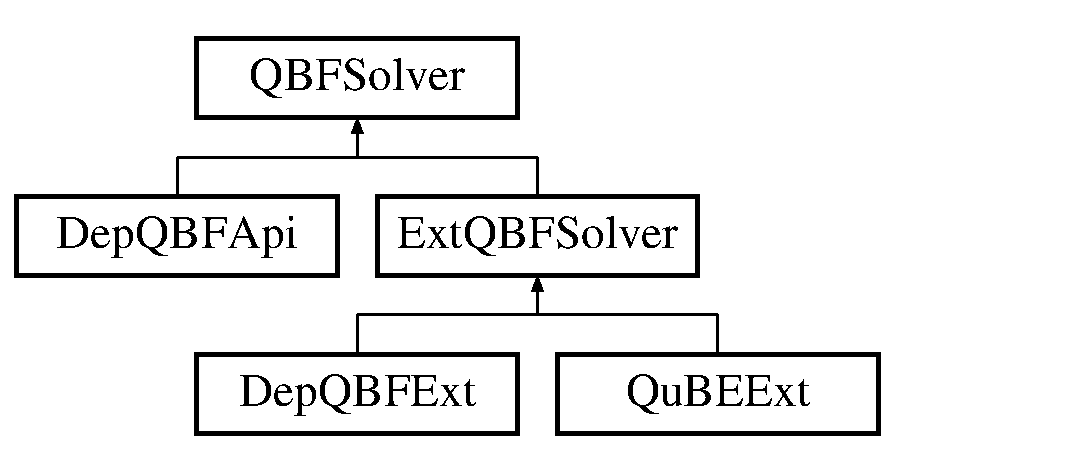
\includegraphics[height=3.000000cm]{classQBFSolver}
\end{center}
\end{figure}
\subsection*{Public Types}
\begin{DoxyCompactItemize}
\item 
enum \hyperlink{classQBFSolver_ac091e263cb55286cc07b2451bcf4d3c7}{Quant} \{ \hyperlink{classQBFSolver_ac091e263cb55286cc07b2451bcf4d3c7a090ab4a5b262710ccd80e97d72f9a7b3}{E}, 
\hyperlink{classQBFSolver_ac091e263cb55286cc07b2451bcf4d3c7afd6518d5d985aa8346ac071e4c0d8ee0}{A}
 \}
\begin{DoxyCompactList}\small\item\em A type for the different kinds of quantifiers. \end{DoxyCompactList}\end{DoxyCompactItemize}
\subsection*{Public Member Functions}
\begin{DoxyCompactItemize}
\item 
\hyperlink{classQBFSolver_ab5a0b6c6cdcbb64a93a9d3dee844ddd3}{Q\-B\-F\-Solver} ()
\begin{DoxyCompactList}\small\item\em Constructor. \end{DoxyCompactList}\item 
virtual \hyperlink{classQBFSolver_a46d8bcb3b6ba6299eea0ae21973d7049}{$\sim$\-Q\-B\-F\-Solver} ()
\begin{DoxyCompactList}\small\item\em Destructor. \end{DoxyCompactList}\item 
virtual bool \hyperlink{classQBFSolver_a53ef157391b176dfbd2a77a1e31befc3}{is\-Sat} (const vector$<$ pair$<$ \hyperlink{classVarInfo_a64d1da76cf84fe674e5fef9764ef11cf}{Var\-Info\-::\-Var\-Kind}, \hyperlink{classQBFSolver_ac091e263cb55286cc07b2451bcf4d3c7}{Quant} $>$ $>$ \&quantifier\-\_\-prefix, const \hyperlink{classCNF}{C\-N\-F} \&cnf)=0
\begin{DoxyCompactList}\small\item\em Checks if a given Q\-B\-F is satisfiable (with quantification over variable kinds). \end{DoxyCompactList}\item 
virtual bool \hyperlink{classQBFSolver_aca37de5801e36d4749b80b6c8c2023a9}{is\-Sat} (const vector$<$ pair$<$ vector$<$ int $>$, \hyperlink{classQBFSolver_ac091e263cb55286cc07b2451bcf4d3c7}{Quant} $>$ $>$ \&quantifier\-\_\-prefix, const \hyperlink{classCNF}{C\-N\-F} \&cnf)=0
\begin{DoxyCompactList}\small\item\em Checks if a given Q\-B\-F is satisfiable (with quantification over variable sets). \end{DoxyCompactList}\item 
virtual bool \hyperlink{classQBFSolver_a76fc0c757a2c039816e3e06547f06d5c}{is\-Sat\-Model} (const vector$<$ pair$<$ \hyperlink{classVarInfo_a64d1da76cf84fe674e5fef9764ef11cf}{Var\-Info\-::\-Var\-Kind}, \hyperlink{classQBFSolver_ac091e263cb55286cc07b2451bcf4d3c7}{Quant} $>$ $>$ \&quantifier\-\_\-prefix, const \hyperlink{classCNF}{C\-N\-F} \&cnf, vector$<$ int $>$ \&model)=0
\begin{DoxyCompactList}\small\item\em Checks satisfiability and extracts a model (quantifying over variable kinds). \end{DoxyCompactList}\item 
virtual bool \hyperlink{classQBFSolver_a12f2ce57b778b9efe729d63bf881493d}{is\-Sat\-Model} (const vector$<$ pair$<$ vector$<$ int $>$, \hyperlink{classQBFSolver_ac091e263cb55286cc07b2451bcf4d3c7}{Quant} $>$ $>$ \&quantifier\-\_\-prefix, const \hyperlink{classCNF}{C\-N\-F} \&cnf, vector$<$ int $>$ \&model)=0
\begin{DoxyCompactList}\small\item\em Checks satisfiability and extracts a model (quantifying over variable sets). \end{DoxyCompactList}\end{DoxyCompactItemize}
\subsection*{Private Member Functions}
\begin{DoxyCompactItemize}
\item 
\hyperlink{classQBFSolver_a37724e17445199de54e0b78307214e78}{Q\-B\-F\-Solver} (const \hyperlink{classQBFSolver}{Q\-B\-F\-Solver} \&other)
\begin{DoxyCompactList}\small\item\em Copy constructor. \end{DoxyCompactList}\item 
\hyperlink{classQBFSolver}{Q\-B\-F\-Solver} \& \hyperlink{classQBFSolver_a0ee7d775a4f07b088924e9e31d800a53}{operator=} (const \hyperlink{classQBFSolver}{Q\-B\-F\-Solver} \&other)
\begin{DoxyCompactList}\small\item\em Assignment operator. \end{DoxyCompactList}\end{DoxyCompactItemize}


\subsection{Detailed Description}
An abstract interface for all Q\-B\-F-\/solver implementations. 

This class represents an abstract interface all Q\-B\-F-\/solver instances. You cannot instantiate objects of this class. You need to instantiate objects of one of the derived classes (e.\-g., \hyperlink{classDepQBFApi}{Dep\-Q\-B\-F\-Api}, \hyperlink{classDepQBFExt}{Dep\-Q\-B\-F\-Ext}, \hyperlink{classQuBEExt}{Qu\-B\-E\-Ext}) instead. For a given Quantified Boolean formula (a \hyperlink{classCNF}{C\-N\-F} with a quantifier prefix), a \hyperlink{classQBFSolver}{Q\-B\-F\-Solver} is able to determine satisfiability. Furthermore, in case of satisfiability, it can extract satisfying assignments for variables quantified existentially on the outermost level. 

Definition at line 49 of file Q\-B\-F\-Solver.\-h.



\subsection{Member Enumeration Documentation}
\hypertarget{classQBFSolver_ac091e263cb55286cc07b2451bcf4d3c7}{\index{Q\-B\-F\-Solver@{Q\-B\-F\-Solver}!Quant@{Quant}}
\index{Quant@{Quant}!QBFSolver@{Q\-B\-F\-Solver}}
\subsubsection[{Quant}]{\setlength{\rightskip}{0pt plus 5cm}enum {\bf Q\-B\-F\-Solver\-::\-Quant}}}\label{classQBFSolver_ac091e263cb55286cc07b2451bcf4d3c7}


A type for the different kinds of quantifiers. 

\begin{Desc}
\item[Enumerator]\par
\begin{description}
\index{E@{E}!Q\-B\-F\-Solver@{Q\-B\-F\-Solver}}\index{Q\-B\-F\-Solver@{Q\-B\-F\-Solver}!E@{E}}\item[{\em 
\hypertarget{classQBFSolver_ac091e263cb55286cc07b2451bcf4d3c7a090ab4a5b262710ccd80e97d72f9a7b3}{E}\label{classQBFSolver_ac091e263cb55286cc07b2451bcf4d3c7a090ab4a5b262710ccd80e97d72f9a7b3}
}]The value for existential quantification. \index{A@{A}!Q\-B\-F\-Solver@{Q\-B\-F\-Solver}}\index{Q\-B\-F\-Solver@{Q\-B\-F\-Solver}!A@{A}}\item[{\em 
\hypertarget{classQBFSolver_ac091e263cb55286cc07b2451bcf4d3c7afd6518d5d985aa8346ac071e4c0d8ee0}{A}\label{classQBFSolver_ac091e263cb55286cc07b2451bcf4d3c7afd6518d5d985aa8346ac071e4c0d8ee0}
}]The value for universal quantification. \end{description}
\end{Desc}


Definition at line 56 of file Q\-B\-F\-Solver.\-h.



\subsection{Constructor \& Destructor Documentation}
\hypertarget{classQBFSolver_ab5a0b6c6cdcbb64a93a9d3dee844ddd3}{\index{Q\-B\-F\-Solver@{Q\-B\-F\-Solver}!Q\-B\-F\-Solver@{Q\-B\-F\-Solver}}
\index{Q\-B\-F\-Solver@{Q\-B\-F\-Solver}!QBFSolver@{Q\-B\-F\-Solver}}
\subsubsection[{Q\-B\-F\-Solver}]{\setlength{\rightskip}{0pt plus 5cm}Q\-B\-F\-Solver\-::\-Q\-B\-F\-Solver (
\begin{DoxyParamCaption}
{}
\end{DoxyParamCaption}
)}}\label{classQBFSolver_ab5a0b6c6cdcbb64a93a9d3dee844ddd3}


Constructor. 



Definition at line 33 of file Q\-B\-F\-Solver.\-cpp.

\hypertarget{classQBFSolver_a46d8bcb3b6ba6299eea0ae21973d7049}{\index{Q\-B\-F\-Solver@{Q\-B\-F\-Solver}!$\sim$\-Q\-B\-F\-Solver@{$\sim$\-Q\-B\-F\-Solver}}
\index{$\sim$\-Q\-B\-F\-Solver@{$\sim$\-Q\-B\-F\-Solver}!QBFSolver@{Q\-B\-F\-Solver}}
\subsubsection[{$\sim$\-Q\-B\-F\-Solver}]{\setlength{\rightskip}{0pt plus 5cm}Q\-B\-F\-Solver\-::$\sim$\-Q\-B\-F\-Solver (
\begin{DoxyParamCaption}
{}
\end{DoxyParamCaption}
)\hspace{0.3cm}{\ttfamily [virtual]}}}\label{classQBFSolver_a46d8bcb3b6ba6299eea0ae21973d7049}


Destructor. 



Definition at line 39 of file Q\-B\-F\-Solver.\-cpp.

\hypertarget{classQBFSolver_a37724e17445199de54e0b78307214e78}{\index{Q\-B\-F\-Solver@{Q\-B\-F\-Solver}!Q\-B\-F\-Solver@{Q\-B\-F\-Solver}}
\index{Q\-B\-F\-Solver@{Q\-B\-F\-Solver}!QBFSolver@{Q\-B\-F\-Solver}}
\subsubsection[{Q\-B\-F\-Solver}]{\setlength{\rightskip}{0pt plus 5cm}Q\-B\-F\-Solver\-::\-Q\-B\-F\-Solver (
\begin{DoxyParamCaption}
\item[{const {\bf Q\-B\-F\-Solver} \&}]{other}
\end{DoxyParamCaption}
)\hspace{0.3cm}{\ttfamily [private]}}}\label{classQBFSolver_a37724e17445199de54e0b78307214e78}


Copy constructor. 

The copy constructor is disabled (set private) and not implemented.


\begin{DoxyParams}{Parameters}
{\em other} & The source for creating the copy. \\
\hline
\end{DoxyParams}


\subsection{Member Function Documentation}
\hypertarget{classQBFSolver_a53ef157391b176dfbd2a77a1e31befc3}{\index{Q\-B\-F\-Solver@{Q\-B\-F\-Solver}!is\-Sat@{is\-Sat}}
\index{is\-Sat@{is\-Sat}!QBFSolver@{Q\-B\-F\-Solver}}
\subsubsection[{is\-Sat}]{\setlength{\rightskip}{0pt plus 5cm}virtual bool Q\-B\-F\-Solver\-::is\-Sat (
\begin{DoxyParamCaption}
\item[{const vector$<$ pair$<$ {\bf Var\-Info\-::\-Var\-Kind}, {\bf Quant} $>$ $>$ \&}]{quantifier\-\_\-prefix, }
\item[{const {\bf C\-N\-F} \&}]{cnf}
\end{DoxyParamCaption}
)\hspace{0.3cm}{\ttfamily [pure virtual]}}}\label{classQBFSolver_a53ef157391b176dfbd2a77a1e31befc3}


Checks if a given Q\-B\-F is satisfiable (with quantification over variable kinds). 

The Q\-B\-F consists of a quantifier prefix and a Boolean formula in \hyperlink{classCNF}{C\-N\-F}. The quantifier prefix assigns an existential or universal quantifier to every kind of variable.

This is an abstract method which must be implemented in all derived classes (all classes implementing this interface).


\begin{DoxyParams}{Parameters}
{\em quantifier\-\_\-prefix} & The quantifier prefix as a vector of pairs. vector\mbox{[}0\mbox{]} is the leftmost (i.\-e., outermost) quantifier block. The pairs in the quantifier\-\_\-prefix assign an existential or universal quantifier to every kind of variable that occurs in the cnf. \\
\hline
{\em cnf} & A Boolean formula in \hyperlink{classCNF}{C\-N\-F}. \\
\hline
\end{DoxyParams}
\begin{DoxyReturn}{Returns}
True if the Q\-B\-F is satisfiable, false otherwise. 
\end{DoxyReturn}


Implemented in \hyperlink{classDepQBFApi_a1f755841365d67f4c704bf919cb4f8b5}{Dep\-Q\-B\-F\-Api}, \hyperlink{classExtQBFSolver_abec25b97170b79b42b85d1d4ec825a39}{Ext\-Q\-B\-F\-Solver}, and \hyperlink{classRareqsApi_a90fa7a7affc2a12a287cea15d7f651c7}{Rareqs\-Api}.



Referenced by Utils\-::debug\-Check\-Win\-Reg(), Learn\-Synth\-Q\-B\-F\-Ind\-::debug\-Check\-Win\-Reg\-Reach(), Learn\-Synth\-Q\-B\-F\-::generalize\-Counterexample(), Learn\-Synth\-Q\-B\-F\-Ind\-::generalize\-Counterexample(), Clause\-Minimizer\-Q\-B\-F\-::minimize\-Clauses\-No\-Inc(), Learn\-Synth\-Q\-B\-F\-::reduce\-Existing\-Clauses(), Learn\-Synth\-Q\-B\-F\-Ind\-::reduce\-Existing\-Clauses(), and Learning\-Impl\-Extractor\-::run\-Learning\-Q\-B\-F().

\hypertarget{classQBFSolver_aca37de5801e36d4749b80b6c8c2023a9}{\index{Q\-B\-F\-Solver@{Q\-B\-F\-Solver}!is\-Sat@{is\-Sat}}
\index{is\-Sat@{is\-Sat}!QBFSolver@{Q\-B\-F\-Solver}}
\subsubsection[{is\-Sat}]{\setlength{\rightskip}{0pt plus 5cm}virtual bool Q\-B\-F\-Solver\-::is\-Sat (
\begin{DoxyParamCaption}
\item[{const vector$<$ pair$<$ vector$<$ int $>$, {\bf Quant} $>$ $>$ \&}]{quantifier\-\_\-prefix, }
\item[{const {\bf C\-N\-F} \&}]{cnf}
\end{DoxyParamCaption}
)\hspace{0.3cm}{\ttfamily [pure virtual]}}}\label{classQBFSolver_aca37de5801e36d4749b80b6c8c2023a9}


Checks if a given Q\-B\-F is satisfiable (with quantification over variable sets). 

The Q\-B\-F consists of a quantifier prefix and a Boolean formula in \hyperlink{classCNF}{C\-N\-F}. The quantifier prefix assigns an existential or universal quantifier to different sets variable.

This is an abstract method which must be implemented in all derived classes (all classes implementing this interface).


\begin{DoxyParams}{Parameters}
{\em quantifier\-\_\-prefix} & The quantifier prefix as a vector of pairs. vector\mbox{[}0\mbox{]} is the leftmost (i.\-e., outermost) quantifier block. The pairs in the quantifier\-\_\-prefix assign an existential or universal quantifier to different sets of variables occurring in the cnf. \\
\hline
{\em cnf} & A Boolean formula in \hyperlink{classCNF}{C\-N\-F}. \\
\hline
\end{DoxyParams}
\begin{DoxyReturn}{Returns}
True if the Q\-B\-F is satisfiable, false otherwise. 
\end{DoxyReturn}


Implemented in \hyperlink{classExtQBFSolver_adc1bacec3307200dd90b260789e4c808}{Ext\-Q\-B\-F\-Solver}, \hyperlink{classDepQBFApi_a8b220fef622b400b37d8298f29826938}{Dep\-Q\-B\-F\-Api}, and \hyperlink{classRareqsApi_a090cdbd8cfe16e475c29240a50f690fe}{Rareqs\-Api}.

\hypertarget{classQBFSolver_a76fc0c757a2c039816e3e06547f06d5c}{\index{Q\-B\-F\-Solver@{Q\-B\-F\-Solver}!is\-Sat\-Model@{is\-Sat\-Model}}
\index{is\-Sat\-Model@{is\-Sat\-Model}!QBFSolver@{Q\-B\-F\-Solver}}
\subsubsection[{is\-Sat\-Model}]{\setlength{\rightskip}{0pt plus 5cm}virtual bool Q\-B\-F\-Solver\-::is\-Sat\-Model (
\begin{DoxyParamCaption}
\item[{const vector$<$ pair$<$ {\bf Var\-Info\-::\-Var\-Kind}, {\bf Quant} $>$ $>$ \&}]{quantifier\-\_\-prefix, }
\item[{const {\bf C\-N\-F} \&}]{cnf, }
\item[{vector$<$ int $>$ \&}]{model}
\end{DoxyParamCaption}
)\hspace{0.3cm}{\ttfamily [pure virtual]}}}\label{classQBFSolver_a76fc0c757a2c039816e3e06547f06d5c}


Checks satisfiability and extracts a model (quantifying over variable kinds). 

Just like \hyperlink{classQBFSolver_a53ef157391b176dfbd2a77a1e31befc3}{is\-Sat() }, this method checks a quantified Boolean formula for satisfiability. If the Q\-B\-F is satisfiable, this method also extracts a model (a satisfying assignment) for all variables which are quantified existentially on the outermost level. The model is provided as cube\-: negated variables in the cube are F\-A\-L\-S\-E, unnegated ones are T\-R\-U\-E.

This is an abstract method which must be implemented in all derived classes (all classes implementing this interface).


\begin{DoxyParams}{Parameters}
{\em quantifier\-\_\-prefix} & The quantifier prefix as a vector of pairs. vector\mbox{[}0\mbox{]} is the leftmost (i.\-e., outermost) quantifier block. The pairs in the quantifier\-\_\-prefix assign an existential or universal quantifier to every kind of variable that occurs in the cnf. \\
\hline
{\em cnf} & A Boolean formula in \hyperlink{classCNF}{C\-N\-F}. \\
\hline
{\em model} & The resulting model in form of a cube in case of satisfiability. Negated variables in the cube are F\-A\-L\-S\-E, unnegated ones are T\-R\-U\-E. If the formula is unsatisfiable (this method returns false) then this parameter is not modified. \\
\hline
\end{DoxyParams}
\begin{DoxyReturn}{Returns}
True if the Q\-B\-F is satisfiable, false otherwise. 
\end{DoxyReturn}


Implemented in \hyperlink{classExtQBFSolver_ad66c53343ce9c03eea6e4b5e7753f1b3}{Ext\-Q\-B\-F\-Solver}, \hyperlink{classDepQBFApi_af70faa0b2136fe04e2a22743f2ca7c8e}{Dep\-Q\-B\-F\-Api}, and \hyperlink{classRareqsApi_a243411cd4a5cc417f9fc12089b8381b8}{Rareqs\-Api}.



Referenced by Learn\-Synth\-Q\-B\-F\-::compute\-Counterexample\-Q\-B\-F(), Learn\-Synth\-Q\-B\-F\-Ind\-::compute\-Counterexample\-Q\-B\-F(), Learning\-Impl\-Extractor\-::run\-Learning\-Q\-B\-F(), and Template\-Synth\-::synt\-Q\-B\-F().

\hypertarget{classQBFSolver_a12f2ce57b778b9efe729d63bf881493d}{\index{Q\-B\-F\-Solver@{Q\-B\-F\-Solver}!is\-Sat\-Model@{is\-Sat\-Model}}
\index{is\-Sat\-Model@{is\-Sat\-Model}!QBFSolver@{Q\-B\-F\-Solver}}
\subsubsection[{is\-Sat\-Model}]{\setlength{\rightskip}{0pt plus 5cm}virtual bool Q\-B\-F\-Solver\-::is\-Sat\-Model (
\begin{DoxyParamCaption}
\item[{const vector$<$ pair$<$ vector$<$ int $>$, {\bf Quant} $>$ $>$ \&}]{quantifier\-\_\-prefix, }
\item[{const {\bf C\-N\-F} \&}]{cnf, }
\item[{vector$<$ int $>$ \&}]{model}
\end{DoxyParamCaption}
)\hspace{0.3cm}{\ttfamily [pure virtual]}}}\label{classQBFSolver_a12f2ce57b778b9efe729d63bf881493d}


Checks satisfiability and extracts a model (quantifying over variable sets). 

Just like \hyperlink{classQBFSolver_a53ef157391b176dfbd2a77a1e31befc3}{is\-Sat() }, this method checks a quantified Boolean formula for satisfiability. If the Q\-B\-F is satisfiable, this method also extracts a model (a satisfying assignment) for all variables which are quantified existentially on the outermost level. The model is provided as cube\-: negated variables in the cube are F\-A\-L\-S\-E, unnegated ones are T\-R\-U\-E.

This is an abstract method which must be implemented in all derived classes (all classes implementing this interface).


\begin{DoxyParams}{Parameters}
{\em quantifier\-\_\-prefix} & The quantifier prefix as a vector of pairs. vector\mbox{[}0\mbox{]} is the leftmost (i.\-e., outermost) quantifier block. The pairs in the quantifier\-\_\-prefix assign an existential or universal quantifier to different sets of variables occurring in the cnf. \\
\hline
{\em cnf} & A Boolean formula in \hyperlink{classCNF}{C\-N\-F}. \\
\hline
{\em model} & The resulting model in form of a cube in case of satisfiability. Negated variables in the cube are F\-A\-L\-S\-E, unnegated ones are T\-R\-U\-E. If the formula is unsatisfiable (this method returns false) then this parameter is not modified. \\
\hline
\end{DoxyParams}
\begin{DoxyReturn}{Returns}
True if the Q\-B\-F is satisfiable, false otherwise. 
\end{DoxyReturn}


Implemented in \hyperlink{classExtQBFSolver_a3add00496f016c2e60a188ce9daa1da1}{Ext\-Q\-B\-F\-Solver}, \hyperlink{classDepQBFApi_a4278bfb0cf01f21e9aa6333e14e4f5af}{Dep\-Q\-B\-F\-Api}, and \hyperlink{classRareqsApi_a70eb2a4b5b5e5493482c6c54ea00b295}{Rareqs\-Api}.

\hypertarget{classQBFSolver_a0ee7d775a4f07b088924e9e31d800a53}{\index{Q\-B\-F\-Solver@{Q\-B\-F\-Solver}!operator=@{operator=}}
\index{operator=@{operator=}!QBFSolver@{Q\-B\-F\-Solver}}
\subsubsection[{operator=}]{\setlength{\rightskip}{0pt plus 5cm}{\bf Q\-B\-F\-Solver}\& Q\-B\-F\-Solver\-::operator= (
\begin{DoxyParamCaption}
\item[{const {\bf Q\-B\-F\-Solver} \&}]{other}
\end{DoxyParamCaption}
)\hspace{0.3cm}{\ttfamily [private]}}}\label{classQBFSolver_a0ee7d775a4f07b088924e9e31d800a53}


Assignment operator. 

The assignment operator is disabled (set private) and not implemented.


\begin{DoxyParams}{Parameters}
{\em other} & The source for creating the copy. \\
\hline
\end{DoxyParams}
\begin{DoxyReturn}{Returns}
The result of the assignment, i.\-e, $\ast$this. 
\end{DoxyReturn}


The documentation for this class was generated from the following files\-:\begin{DoxyCompactItemize}
\item 
src/\hyperlink{QBFSolver_8h}{Q\-B\-F\-Solver.\-h}\item 
src/\hyperlink{QBFSolver_8cpp}{Q\-B\-F\-Solver.\-cpp}\end{DoxyCompactItemize}

\hypertarget{classQuBEExt}{\section{Qu\-B\-E\-Ext Class Reference}
\label{classQuBEExt}\index{Qu\-B\-E\-Ext@{Qu\-B\-E\-Ext}}
}


Calls the Qu\-B\-E Q\-B\-F-\/solver in a separate process, communicating with files.  




{\ttfamily \#include $<$Qu\-B\-E\-Ext.\-h$>$}

Inheritance diagram for Qu\-B\-E\-Ext\-:\begin{figure}[H]
\begin{center}
\leavevmode
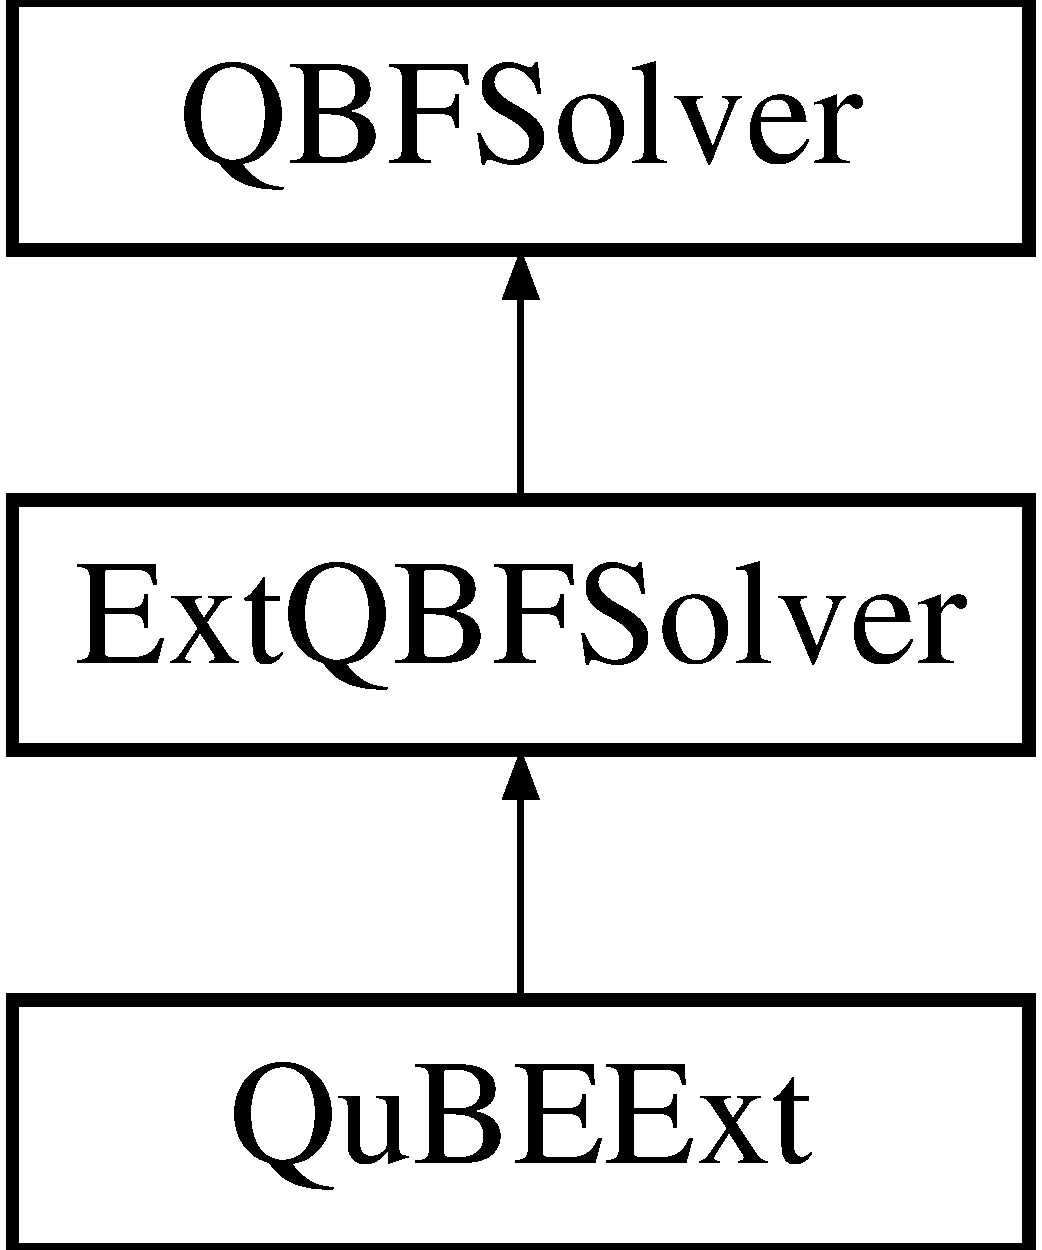
\includegraphics[height=3.000000cm]{classQuBEExt}
\end{center}
\end{figure}
\subsection*{Public Types}
\begin{DoxyCompactItemize}
\item 
enum \hyperlink{classQBFSolver_ac091e263cb55286cc07b2451bcf4d3c7}{Quant} \{ \hyperlink{classQBFSolver_ac091e263cb55286cc07b2451bcf4d3c7a090ab4a5b262710ccd80e97d72f9a7b3}{E}, 
\hyperlink{classQBFSolver_ac091e263cb55286cc07b2451bcf4d3c7afd6518d5d985aa8346ac071e4c0d8ee0}{A}
 \}
\begin{DoxyCompactList}\small\item\em A type for the different kinds of quantifiers. \end{DoxyCompactList}\end{DoxyCompactItemize}
\subsection*{Public Member Functions}
\begin{DoxyCompactItemize}
\item 
\hyperlink{classQuBEExt_ab433b787109ae43f6e42dbed855bc6fa}{Qu\-B\-E\-Ext} ()
\begin{DoxyCompactList}\small\item\em Constructor. \end{DoxyCompactList}\item 
virtual \hyperlink{classQuBEExt_a0e070d528067724a14f2835b751d41cd}{$\sim$\-Qu\-B\-E\-Ext} ()
\begin{DoxyCompactList}\small\item\em Destructor. \end{DoxyCompactList}\item 
virtual bool \hyperlink{classExtQBFSolver_abec25b97170b79b42b85d1d4ec825a39}{is\-Sat} (const vector$<$ pair$<$ \hyperlink{classVarInfo_a64d1da76cf84fe674e5fef9764ef11cf}{Var\-Info\-::\-Var\-Kind}, \hyperlink{classQBFSolver_ac091e263cb55286cc07b2451bcf4d3c7}{Quant} $>$ $>$ \&quantifier\-\_\-prefix, const \hyperlink{classCNF}{C\-N\-F} \&cnf)
\begin{DoxyCompactList}\small\item\em Checks if a given Q\-B\-F is satisfiable (with quantification over variable kinds). \end{DoxyCompactList}\item 
virtual bool \hyperlink{classExtQBFSolver_adc1bacec3307200dd90b260789e4c808}{is\-Sat} (const vector$<$ pair$<$ vector$<$ int $>$, \hyperlink{classQBFSolver_ac091e263cb55286cc07b2451bcf4d3c7}{Quant} $>$ $>$ \&quantifier\-\_\-prefix, const \hyperlink{classCNF}{C\-N\-F} \&cnf)
\begin{DoxyCompactList}\small\item\em Checks if a given Q\-B\-F is satisfiable (with quantification over variable sets). \end{DoxyCompactList}\item 
virtual bool \hyperlink{classExtQBFSolver_ad66c53343ce9c03eea6e4b5e7753f1b3}{is\-Sat\-Model} (const vector$<$ pair$<$ \hyperlink{classVarInfo_a64d1da76cf84fe674e5fef9764ef11cf}{Var\-Info\-::\-Var\-Kind}, \hyperlink{classQBFSolver_ac091e263cb55286cc07b2451bcf4d3c7}{Quant} $>$ $>$ \&quantifier\-\_\-prefix, const \hyperlink{classCNF}{C\-N\-F} \&cnf, vector$<$ int $>$ \&model)
\begin{DoxyCompactList}\small\item\em Checks satisfiability and extracts a model (quantifying over variable kinds). \end{DoxyCompactList}\item 
virtual bool \hyperlink{classExtQBFSolver_a3add00496f016c2e60a188ce9daa1da1}{is\-Sat\-Model} (const vector$<$ pair$<$ vector$<$ int $>$, \hyperlink{classQBFSolver_ac091e263cb55286cc07b2451bcf4d3c7}{Quant} $>$ $>$ \&quantifier\-\_\-prefix, const \hyperlink{classCNF}{C\-N\-F} \&cnf, vector$<$ int $>$ \&model)
\begin{DoxyCompactList}\small\item\em Checks satisfiability and extracts a model (quantifying over variable sets). \end{DoxyCompactList}\end{DoxyCompactItemize}
\subsection*{Static Public Member Functions}
\begin{DoxyCompactItemize}
\item 
static void \hyperlink{classExtQBFSolver_abebb2acbb5afd5b205254246f39f3e33}{dump\-Q\-B\-F} (const vector$<$ pair$<$ \hyperlink{classVarInfo_a64d1da76cf84fe674e5fef9764ef11cf}{Var\-Info\-::\-Var\-Kind}, \hyperlink{classQBFSolver_ac091e263cb55286cc07b2451bcf4d3c7}{Quant} $>$ $>$ \&quantifier\-\_\-prefix, const \hyperlink{classCNF}{C\-N\-F} \&cnf, const string \&filename)
\begin{DoxyCompactList}\small\item\em Dumps a Q\-B\-F (quantification over variable kinds) into a file in Q\-D\-I\-M\-A\-C\-S format. \end{DoxyCompactList}\item 
static void \hyperlink{classExtQBFSolver_a7e329d1fdce2cf65390930b01cf3a32b}{dump\-Q\-B\-F} (const vector$<$ pair$<$ vector$<$ int $>$, \hyperlink{classQBFSolver_ac091e263cb55286cc07b2451bcf4d3c7}{Quant} $>$ $>$ \&quantifier\-\_\-prefix, const \hyperlink{classCNF}{C\-N\-F} \&cnf, const string \&filename)
\begin{DoxyCompactList}\small\item\em Dumps a Q\-B\-F (quantification over variable kinds) into a file in Q\-D\-I\-M\-A\-C\-S format. \end{DoxyCompactList}\end{DoxyCompactItemize}
\subsection*{Protected Member Functions}
\begin{DoxyCompactItemize}
\item 
virtual string \hyperlink{classQuBEExt_a2af26a63952d83a50a4bd3d72bfc572a}{get\-Solver\-Command} () const 
\begin{DoxyCompactList}\small\item\em Returns the command to execute Qu\-B\-E. \end{DoxyCompactList}\item 
virtual string \hyperlink{classQuBEExt_a846ea873ec83e57213f1931d85cb8bd0}{get\-Solver\-Command\-Model} () const 
\begin{DoxyCompactList}\small\item\em Returns the command to execute Dep\-Q\-B\-F such that it produces models. \end{DoxyCompactList}\item 
virtual bool \hyperlink{classExtQBFSolver_a11ddbf3980824453238071e8a036f804}{parse\-Answer} (int ret) const 
\begin{DoxyCompactList}\small\item\em Parses the answer of the Q\-B\-F solver to get the satisfiability verdict. \end{DoxyCompactList}\item 
virtual bool \hyperlink{classExtQBFSolver_a3b43f437ee9286b62be1de73932b6636}{parse\-Model} (int ret, vector$<$ int $>$ \&model) const 
\begin{DoxyCompactList}\small\item\em Parses the answer of the Q\-B\-F solver to get the satisfiability verdict and a model. \end{DoxyCompactList}\item 
virtual void \hyperlink{classExtQBFSolver_a3ee48837c5e937e4d3a5b3c2a6b761d3}{cleanup} ()
\begin{DoxyCompactList}\small\item\em Deletes the temporary files that have been used for communication. \end{DoxyCompactList}\end{DoxyCompactItemize}
\subsection*{Protected Attributes}
\begin{DoxyCompactItemize}
\item 
string \hyperlink{classQuBEExt_a02646118beb978edff16fc0094a798f8}{path\-\_\-to\-\_\-qube\-\_\-}
\begin{DoxyCompactList}\small\item\em The path to the Qu\-B\-E executable. \end{DoxyCompactList}\item 
string \hyperlink{classQuBEExt_aed89db58647a80a6204798720ec136df}{path\-\_\-to\-\_\-deqqbf\-\_\-}
\begin{DoxyCompactList}\small\item\em The path to the Dep\-Q\-B\-F executable. \end{DoxyCompactList}\item 
string \hyperlink{classExtQBFSolver_a04d2ff483c22a11344e46d66ae7e76b1}{in\-\_\-file\-\_\-name\-\_\-}
\begin{DoxyCompactList}\small\item\em The name of the Q\-D\-I\-M\-A\-C\-S file containing the Q\-B\-F to be solved. \end{DoxyCompactList}\item 
string \hyperlink{classExtQBFSolver_a0efb35aa9b807dec521ad3406eaf664d}{out\-\_\-file\-\_\-name\-\_\-}
\begin{DoxyCompactList}\small\item\em The name of the file that is produced by the Q\-B\-F-\/solver (containing the model). \end{DoxyCompactList}\end{DoxyCompactItemize}
\subsection*{Private Member Functions}
\begin{DoxyCompactItemize}
\item 
\hyperlink{classQuBEExt_aee6b5faa4e71bef7df5f0961f8de31d7}{Qu\-B\-E\-Ext} (const \hyperlink{classQuBEExt}{Qu\-B\-E\-Ext} \&other)
\begin{DoxyCompactList}\small\item\em Copy constructor. \end{DoxyCompactList}\item 
\hyperlink{classQuBEExt}{Qu\-B\-E\-Ext} \& \hyperlink{classQuBEExt_ae9f834011d3dd5ef0452b70052e10bd0}{operator=} (const \hyperlink{classQuBEExt}{Qu\-B\-E\-Ext} \&other)
\begin{DoxyCompactList}\small\item\em Assignment operator. \end{DoxyCompactList}\end{DoxyCompactItemize}


\subsection{Detailed Description}
Calls the Qu\-B\-E Q\-B\-F-\/solver in a separate process, communicating with files. 

This class represents an interface to the Q\-B\-F-\/solver Qu\-B\-E (see www.\-star-\/lab.\-it/$\sim$qube/). For a given Quantified Boolean formula (a \hyperlink{classCNF}{C\-N\-F} with a quantifier prefix), this class is able to determine satisfiability. Furthermore, in case of satisfiability, it can extract satisfying assignments for variables quantified existentially on the outermost level. The Qu\-B\-E solver is executed in a separate process. Communication with this process works via files. Qu\-B\-E can only decide the satisfiability of a formula, but it cannot produce satisfying assignments. Hence, if a satisfying assignment is needed, we simply delegate the call to Dep\-Q\-B\-F.

Most of work is actually implemented in the base class \hyperlink{classExtQBFSolver}{Ext\-Q\-B\-F\-Solver}. This class mainly overrides some methods which are specific for Qu\-B\-E.

\begin{DoxyAuthor}{Author}
Robert Koenighofer (\href{mailto:robert.koenighofer@iaik.tugraz.at}{\tt robert.\-koenighofer@iaik.\-tugraz.\-at}) 
\end{DoxyAuthor}
\begin{DoxyVersion}{Version}
1.\-1.\-0 
\end{DoxyVersion}


Definition at line 56 of file Qu\-B\-E\-Ext.\-h.



\subsection{Member Enumeration Documentation}
\hypertarget{classQBFSolver_ac091e263cb55286cc07b2451bcf4d3c7}{\index{Qu\-B\-E\-Ext@{Qu\-B\-E\-Ext}!Quant@{Quant}}
\index{Quant@{Quant}!QuBEExt@{Qu\-B\-E\-Ext}}
\subsubsection[{Quant}]{\setlength{\rightskip}{0pt plus 5cm}enum {\bf Q\-B\-F\-Solver\-::\-Quant}\hspace{0.3cm}{\ttfamily [inherited]}}}\label{classQBFSolver_ac091e263cb55286cc07b2451bcf4d3c7}


A type for the different kinds of quantifiers. 

\begin{Desc}
\item[Enumerator\-: ]\par
\begin{description}
\index{E@{E}!Qu\-B\-E\-Ext@{Qu\-B\-E\-Ext}}\index{Qu\-B\-E\-Ext@{Qu\-B\-E\-Ext}!E@{E}}\item[{\em 
\hypertarget{classQBFSolver_ac091e263cb55286cc07b2451bcf4d3c7a090ab4a5b262710ccd80e97d72f9a7b3}{E}\label{classQBFSolver_ac091e263cb55286cc07b2451bcf4d3c7a090ab4a5b262710ccd80e97d72f9a7b3}
}]The value for existential quantification. \index{A@{A}!Qu\-B\-E\-Ext@{Qu\-B\-E\-Ext}}\index{Qu\-B\-E\-Ext@{Qu\-B\-E\-Ext}!A@{A}}\item[{\em 
\hypertarget{classQBFSolver_ac091e263cb55286cc07b2451bcf4d3c7afd6518d5d985aa8346ac071e4c0d8ee0}{A}\label{classQBFSolver_ac091e263cb55286cc07b2451bcf4d3c7afd6518d5d985aa8346ac071e4c0d8ee0}
}]The value for universal quantification. \end{description}
\end{Desc}



Definition at line 56 of file Q\-B\-F\-Solver.\-h.



\subsection{Constructor \& Destructor Documentation}
\hypertarget{classQuBEExt_ab433b787109ae43f6e42dbed855bc6fa}{\index{Qu\-B\-E\-Ext@{Qu\-B\-E\-Ext}!Qu\-B\-E\-Ext@{Qu\-B\-E\-Ext}}
\index{Qu\-B\-E\-Ext@{Qu\-B\-E\-Ext}!QuBEExt@{Qu\-B\-E\-Ext}}
\subsubsection[{Qu\-B\-E\-Ext}]{\setlength{\rightskip}{0pt plus 5cm}Qu\-B\-E\-Ext\-::\-Qu\-B\-E\-Ext (
\begin{DoxyParamCaption}
{}
\end{DoxyParamCaption}
)}}\label{classQuBEExt_ab433b787109ae43f6e42dbed855bc6fa}


Constructor. 



Definition at line 36 of file Qu\-B\-E\-Ext.\-cpp.



References Options\-::get\-T\-P\-Dir\-Name(), Options\-::instance(), M\-A\-S\-S\-E\-R\-T, path\-\_\-to\-\_\-deqqbf\-\_\-, and path\-\_\-to\-\_\-qube\-\_\-.

\hypertarget{classQuBEExt_a0e070d528067724a14f2835b751d41cd}{\index{Qu\-B\-E\-Ext@{Qu\-B\-E\-Ext}!$\sim$\-Qu\-B\-E\-Ext@{$\sim$\-Qu\-B\-E\-Ext}}
\index{$\sim$\-Qu\-B\-E\-Ext@{$\sim$\-Qu\-B\-E\-Ext}!QuBEExt@{Qu\-B\-E\-Ext}}
\subsubsection[{$\sim$\-Qu\-B\-E\-Ext}]{\setlength{\rightskip}{0pt plus 5cm}Qu\-B\-E\-Ext\-::$\sim$\-Qu\-B\-E\-Ext (
\begin{DoxyParamCaption}
{}
\end{DoxyParamCaption}
)\hspace{0.3cm}{\ttfamily [virtual]}}}\label{classQuBEExt_a0e070d528067724a14f2835b751d41cd}


Destructor. 



Definition at line 45 of file Qu\-B\-E\-Ext.\-cpp.

\hypertarget{classQuBEExt_aee6b5faa4e71bef7df5f0961f8de31d7}{\index{Qu\-B\-E\-Ext@{Qu\-B\-E\-Ext}!Qu\-B\-E\-Ext@{Qu\-B\-E\-Ext}}
\index{Qu\-B\-E\-Ext@{Qu\-B\-E\-Ext}!QuBEExt@{Qu\-B\-E\-Ext}}
\subsubsection[{Qu\-B\-E\-Ext}]{\setlength{\rightskip}{0pt plus 5cm}Qu\-B\-E\-Ext\-::\-Qu\-B\-E\-Ext (
\begin{DoxyParamCaption}
\item[{const {\bf Qu\-B\-E\-Ext} \&}]{other}
\end{DoxyParamCaption}
)\hspace{0.3cm}{\ttfamily [private]}}}\label{classQuBEExt_aee6b5faa4e71bef7df5f0961f8de31d7}


Copy constructor. 

The copy constructor is disabled (set private) and not implemented.


\begin{DoxyParams}{Parameters}
{\em other} & The source for creating the copy. \\
\hline
\end{DoxyParams}


\subsection{Member Function Documentation}
\hypertarget{classExtQBFSolver_a3ee48837c5e937e4d3a5b3c2a6b761d3}{\index{Qu\-B\-E\-Ext@{Qu\-B\-E\-Ext}!cleanup@{cleanup}}
\index{cleanup@{cleanup}!QuBEExt@{Qu\-B\-E\-Ext}}
\subsubsection[{cleanup}]{\setlength{\rightskip}{0pt plus 5cm}void Ext\-Q\-B\-F\-Solver\-::cleanup (
\begin{DoxyParamCaption}
{}
\end{DoxyParamCaption}
)\hspace{0.3cm}{\ttfamily [protected]}, {\ttfamily [virtual]}, {\ttfamily [inherited]}}}\label{classExtQBFSolver_a3ee48837c5e937e4d3a5b3c2a6b761d3}


Deletes the temporary files that have been used for communication. 



Definition at line 214 of file Ext\-Q\-B\-F\-Solver.\-cpp.



References Ext\-Q\-B\-F\-Solver\-::in\-\_\-file\-\_\-name\-\_\-, and Ext\-Q\-B\-F\-Solver\-::out\-\_\-file\-\_\-name\-\_\-.



Referenced by Ext\-Q\-B\-F\-Solver\-::is\-Sat(), Ext\-Q\-B\-F\-Solver\-::is\-Sat\-Model(), and Dep\-Q\-B\-F\-Ext\-::qbf\-Cert().

\hypertarget{classExtQBFSolver_abebb2acbb5afd5b205254246f39f3e33}{\index{Qu\-B\-E\-Ext@{Qu\-B\-E\-Ext}!dump\-Q\-B\-F@{dump\-Q\-B\-F}}
\index{dump\-Q\-B\-F@{dump\-Q\-B\-F}!QuBEExt@{Qu\-B\-E\-Ext}}
\subsubsection[{dump\-Q\-B\-F}]{\setlength{\rightskip}{0pt plus 5cm}void Ext\-Q\-B\-F\-Solver\-::dump\-Q\-B\-F (
\begin{DoxyParamCaption}
\item[{const vector$<$ pair$<$ {\bf Var\-Info\-::\-Var\-Kind}, {\bf Quant} $>$ $>$ \&}]{quantifier\-\_\-prefix, }
\item[{const {\bf C\-N\-F} \&}]{cnf, }
\item[{const string \&}]{filename}
\end{DoxyParamCaption}
)\hspace{0.3cm}{\ttfamily [static]}, {\ttfamily [inherited]}}}\label{classExtQBFSolver_abebb2acbb5afd5b205254246f39f3e33}


Dumps a Q\-B\-F (quantification over variable kinds) into a file in Q\-D\-I\-M\-A\-C\-S format. 


\begin{DoxyParams}{Parameters}
{\em quantifier\-\_\-prefix} & The quantifier prefix as a vector of pairs. vector\mbox{[}0\mbox{]} is the leftmost (i.\-e., outermost) quantifier block. The pairs in the quantifier\-\_\-prefix assign an existential or universal quantifier to every kind of variable that occurs in the cnf. \\
\hline
{\em cnf} & A Boolean formula in \hyperlink{classCNF}{C\-N\-F}. \\
\hline
{\em filename} & The name of the file (including path) to write to. \\
\hline
\end{DoxyParams}


Definition at line 104 of file Ext\-Q\-B\-F\-Solver.\-cpp.



References Q\-B\-F\-Solver\-::\-E, Var\-Manager\-::get\-Max\-C\-N\-F\-Var(), C\-N\-F\-::get\-Nr\-Of\-Clauses(), Var\-Manager\-::get\-Vars\-Of\-Type(), Var\-Manager\-::instance(), and C\-N\-F\-::to\-String().



Referenced by Dep\-Q\-B\-F\-Api\-::debug\-Check\-Bloqqer\-Model(), Dep\-Q\-B\-F\-Api\-::debug\-Check\-Bloqqer\-Verdict(), Ext\-Q\-B\-F\-Solver\-::is\-Sat(), Ext\-Q\-B\-F\-Solver\-::is\-Sat\-Model(), and Dep\-Q\-B\-F\-Ext\-::qbf\-Cert().

\hypertarget{classExtQBFSolver_a7e329d1fdce2cf65390930b01cf3a32b}{\index{Qu\-B\-E\-Ext@{Qu\-B\-E\-Ext}!dump\-Q\-B\-F@{dump\-Q\-B\-F}}
\index{dump\-Q\-B\-F@{dump\-Q\-B\-F}!QuBEExt@{Qu\-B\-E\-Ext}}
\subsubsection[{dump\-Q\-B\-F}]{\setlength{\rightskip}{0pt plus 5cm}void Ext\-Q\-B\-F\-Solver\-::dump\-Q\-B\-F (
\begin{DoxyParamCaption}
\item[{const vector$<$ pair$<$ vector$<$ int $>$, {\bf Quant} $>$ $>$ \&}]{quantifier\-\_\-prefix, }
\item[{const {\bf C\-N\-F} \&}]{cnf, }
\item[{const string \&}]{filename}
\end{DoxyParamCaption}
)\hspace{0.3cm}{\ttfamily [static]}, {\ttfamily [inherited]}}}\label{classExtQBFSolver_a7e329d1fdce2cf65390930b01cf3a32b}


Dumps a Q\-B\-F (quantification over variable kinds) into a file in Q\-D\-I\-M\-A\-C\-S format. 


\begin{DoxyParams}{Parameters}
{\em quantifier\-\_\-prefix} & The quantifier prefix as a vector of pairs. vector\mbox{[}0\mbox{]} is the leftmost (i.\-e., outermost) quantifier block. The pairs in the quantifier\-\_\-prefix assign an existential or universal quantifier to different sets of variables occurring in the cnf. \\
\hline
{\em cnf} & A Boolean formula in \hyperlink{classCNF}{C\-N\-F}. \\
\hline
{\em filename} & The name of the file (including path) to write to. \\
\hline
\end{DoxyParams}


Definition at line 137 of file Ext\-Q\-B\-F\-Solver.\-cpp.



References Q\-B\-F\-Solver\-::\-E, C\-N\-F\-::get\-Nr\-Of\-Clauses(), and C\-N\-F\-::to\-String().

\hypertarget{classQuBEExt_a2af26a63952d83a50a4bd3d72bfc572a}{\index{Qu\-B\-E\-Ext@{Qu\-B\-E\-Ext}!get\-Solver\-Command@{get\-Solver\-Command}}
\index{get\-Solver\-Command@{get\-Solver\-Command}!QuBEExt@{Qu\-B\-E\-Ext}}
\subsubsection[{get\-Solver\-Command}]{\setlength{\rightskip}{0pt plus 5cm}string Qu\-B\-E\-Ext\-::get\-Solver\-Command (
\begin{DoxyParamCaption}
{}
\end{DoxyParamCaption}
) const\hspace{0.3cm}{\ttfamily [protected]}, {\ttfamily [virtual]}}}\label{classQuBEExt_a2af26a63952d83a50a4bd3d72bfc572a}


Returns the command to execute Qu\-B\-E. 

\begin{DoxyReturn}{Returns}
The command to execute Qu\-B\-E. 
\end{DoxyReturn}


Implements \hyperlink{classExtQBFSolver_aec4c2d830f72283e2fbabf4a3f62a640}{Ext\-Q\-B\-F\-Solver}.



Definition at line 51 of file Qu\-B\-E\-Ext.\-cpp.



References Ext\-Q\-B\-F\-Solver\-::in\-\_\-file\-\_\-name\-\_\-, Ext\-Q\-B\-F\-Solver\-::out\-\_\-file\-\_\-name\-\_\-, and path\-\_\-to\-\_\-qube\-\_\-.

\hypertarget{classQuBEExt_a846ea873ec83e57213f1931d85cb8bd0}{\index{Qu\-B\-E\-Ext@{Qu\-B\-E\-Ext}!get\-Solver\-Command\-Model@{get\-Solver\-Command\-Model}}
\index{get\-Solver\-Command\-Model@{get\-Solver\-Command\-Model}!QuBEExt@{Qu\-B\-E\-Ext}}
\subsubsection[{get\-Solver\-Command\-Model}]{\setlength{\rightskip}{0pt plus 5cm}string Qu\-B\-E\-Ext\-::get\-Solver\-Command\-Model (
\begin{DoxyParamCaption}
{}
\end{DoxyParamCaption}
) const\hspace{0.3cm}{\ttfamily [protected]}, {\ttfamily [virtual]}}}\label{classQuBEExt_a846ea873ec83e57213f1931d85cb8bd0}


Returns the command to execute Dep\-Q\-B\-F such that it produces models. 

This is not a copy-\/past error in this comment. We really execute Dep\-Q\-B\-F because Qu\-B\-E cannot produce models.

\begin{DoxyReturn}{Returns}
The command to execute Dep\-Q\-B\-F such that it produces models. 
\end{DoxyReturn}


Implements \hyperlink{classExtQBFSolver_ac2bc9e4817cfa1a54195d7d9f1c7d3bd}{Ext\-Q\-B\-F\-Solver}.



Definition at line 57 of file Qu\-B\-E\-Ext.\-cpp.



References Ext\-Q\-B\-F\-Solver\-::in\-\_\-file\-\_\-name\-\_\-, Ext\-Q\-B\-F\-Solver\-::out\-\_\-file\-\_\-name\-\_\-, and path\-\_\-to\-\_\-deqqbf\-\_\-.

\hypertarget{classExtQBFSolver_abec25b97170b79b42b85d1d4ec825a39}{\index{Qu\-B\-E\-Ext@{Qu\-B\-E\-Ext}!is\-Sat@{is\-Sat}}
\index{is\-Sat@{is\-Sat}!QuBEExt@{Qu\-B\-E\-Ext}}
\subsubsection[{is\-Sat}]{\setlength{\rightskip}{0pt plus 5cm}bool Ext\-Q\-B\-F\-Solver\-::is\-Sat (
\begin{DoxyParamCaption}
\item[{const vector$<$ pair$<$ {\bf Var\-Info\-::\-Var\-Kind}, {\bf Quant} $>$ $>$ \&}]{quantifier\-\_\-prefix, }
\item[{const {\bf C\-N\-F} \&}]{cnf}
\end{DoxyParamCaption}
)\hspace{0.3cm}{\ttfamily [virtual]}, {\ttfamily [inherited]}}}\label{classExtQBFSolver_abec25b97170b79b42b85d1d4ec825a39}


Checks if a given Q\-B\-F is satisfiable (with quantification over variable kinds). 

The Q\-B\-F consists of a quantifier prefix and a Boolean formula in \hyperlink{classCNF}{C\-N\-F}. The quantifier prefix assigns an existential or universal quantifier to every kind of variable. The Q\-B\-F is dumped into a file, a Q\-B\-F-\/solver is called, and the exit code is used to infer the satisfiability result.


\begin{DoxyParams}{Parameters}
{\em quantifier\-\_\-prefix} & The quantifier prefix as a vector of pairs. vector\mbox{[}0\mbox{]} is the leftmost (i.\-e., outermost) quantifier block. The pairs in the quantifier\-\_\-prefix assign an existential or universal quantifier to every kind of variable that occurs in the cnf. \\
\hline
{\em cnf} & A Boolean formula in \hyperlink{classCNF}{C\-N\-F}. \\
\hline
\end{DoxyParams}
\begin{DoxyReturn}{Returns}
True if the Q\-B\-F is satisfiable, false otherwise. 
\end{DoxyReturn}


Implements \hyperlink{classQBFSolver_a53ef157391b176dfbd2a77a1e31befc3}{Q\-B\-F\-Solver}.



Definition at line 54 of file Ext\-Q\-B\-F\-Solver.\-cpp.



References Ext\-Q\-B\-F\-Solver\-::cleanup(), Ext\-Q\-B\-F\-Solver\-::dump\-Q\-B\-F(), Ext\-Q\-B\-F\-Solver\-::get\-Solver\-Command(), Ext\-Q\-B\-F\-Solver\-::in\-\_\-file\-\_\-name\-\_\-, and Ext\-Q\-B\-F\-Solver\-::parse\-Answer().



Referenced by Q\-B\-F\-Cert\-Impl\-Extractor\-::run().

\hypertarget{classExtQBFSolver_adc1bacec3307200dd90b260789e4c808}{\index{Qu\-B\-E\-Ext@{Qu\-B\-E\-Ext}!is\-Sat@{is\-Sat}}
\index{is\-Sat@{is\-Sat}!QuBEExt@{Qu\-B\-E\-Ext}}
\subsubsection[{is\-Sat}]{\setlength{\rightskip}{0pt plus 5cm}bool Ext\-Q\-B\-F\-Solver\-::is\-Sat (
\begin{DoxyParamCaption}
\item[{const vector$<$ pair$<$ vector$<$ int $>$, {\bf Quant} $>$ $>$ \&}]{quantifier\-\_\-prefix, }
\item[{const {\bf C\-N\-F} \&}]{cnf}
\end{DoxyParamCaption}
)\hspace{0.3cm}{\ttfamily [virtual]}, {\ttfamily [inherited]}}}\label{classExtQBFSolver_adc1bacec3307200dd90b260789e4c808}


Checks if a given Q\-B\-F is satisfiable (with quantification over variable sets). 

The Q\-B\-F consists of a quantifier prefix and a Boolean formula in \hyperlink{classCNF}{C\-N\-F}. The quantifier prefix assigns an existential or universal quantifier to different sets variable. The Q\-B\-F is dumped into a file, a Q\-B\-F-\/solver is called, and the exit code is used to infer the satisfiability result.


\begin{DoxyParams}{Parameters}
{\em quantifier\-\_\-prefix} & The quantifier prefix as a vector of pairs. vector\mbox{[}0\mbox{]} is the leftmost (i.\-e., outermost) quantifier block. The pairs in the quantifier\-\_\-prefix assign an existential or universal quantifier to different sets of variables occurring in the cnf. \\
\hline
{\em cnf} & A Boolean formula in \hyperlink{classCNF}{C\-N\-F}. \\
\hline
\end{DoxyParams}
\begin{DoxyReturn}{Returns}
True if the Q\-B\-F is satisfiable, false otherwise. 
\end{DoxyReturn}


Implements \hyperlink{classQBFSolver_aca37de5801e36d4749b80b6c8c2023a9}{Q\-B\-F\-Solver}.



Definition at line 66 of file Ext\-Q\-B\-F\-Solver.\-cpp.



References Ext\-Q\-B\-F\-Solver\-::cleanup(), Ext\-Q\-B\-F\-Solver\-::dump\-Q\-B\-F(), Ext\-Q\-B\-F\-Solver\-::get\-Solver\-Command(), Ext\-Q\-B\-F\-Solver\-::in\-\_\-file\-\_\-name\-\_\-, and Ext\-Q\-B\-F\-Solver\-::parse\-Answer().

\hypertarget{classExtQBFSolver_ad66c53343ce9c03eea6e4b5e7753f1b3}{\index{Qu\-B\-E\-Ext@{Qu\-B\-E\-Ext}!is\-Sat\-Model@{is\-Sat\-Model}}
\index{is\-Sat\-Model@{is\-Sat\-Model}!QuBEExt@{Qu\-B\-E\-Ext}}
\subsubsection[{is\-Sat\-Model}]{\setlength{\rightskip}{0pt plus 5cm}bool Ext\-Q\-B\-F\-Solver\-::is\-Sat\-Model (
\begin{DoxyParamCaption}
\item[{const vector$<$ pair$<$ {\bf Var\-Info\-::\-Var\-Kind}, {\bf Quant} $>$ $>$ \&}]{quantifier\-\_\-prefix, }
\item[{const {\bf C\-N\-F} \&}]{cnf, }
\item[{vector$<$ int $>$ \&}]{model}
\end{DoxyParamCaption}
)\hspace{0.3cm}{\ttfamily [virtual]}, {\ttfamily [inherited]}}}\label{classExtQBFSolver_ad66c53343ce9c03eea6e4b5e7753f1b3}


Checks satisfiability and extracts a model (quantifying over variable kinds). 

Just like \hyperlink{classExtQBFSolver_abec25b97170b79b42b85d1d4ec825a39}{is\-Sat() }, this method checks a quantified Boolean formula for satisfiability. If the Q\-B\-F is satisfiable, this method also extracts a model (a satisfying assignment) for all variables which are quantified existentially on the outermost level. The model is provided as cube\-: negated variables in the cube are F\-A\-L\-S\-E, unnegated ones are T\-R\-U\-E.


\begin{DoxyParams}{Parameters}
{\em quantifier\-\_\-prefix} & The quantifier prefix as a vector of pairs. vector\mbox{[}0\mbox{]} is the leftmost (i.\-e., outermost) quantifier block. The pairs in the quantifier\-\_\-prefix assign an existential or universal quantifier to every kind of variable that occurs in the cnf. \\
\hline
{\em cnf} & A Boolean formula in \hyperlink{classCNF}{C\-N\-F}. \\
\hline
{\em model} & The resulting model in form of a cube in case of satisfiability. Negated variables in the cube are F\-A\-L\-S\-E, unnegated ones are T\-R\-U\-E. If the formula is unsatisfiable (this method returns false) then this parameter is not modified. \\
\hline
\end{DoxyParams}
\begin{DoxyReturn}{Returns}
True if the Q\-B\-F is satisfiable, false otherwise. 
\end{DoxyReturn}


Implements \hyperlink{classQBFSolver_a76fc0c757a2c039816e3e06547f06d5c}{Q\-B\-F\-Solver}.



Definition at line 78 of file Ext\-Q\-B\-F\-Solver.\-cpp.



References Ext\-Q\-B\-F\-Solver\-::cleanup(), Ext\-Q\-B\-F\-Solver\-::dump\-Q\-B\-F(), Ext\-Q\-B\-F\-Solver\-::get\-Solver\-Command\-Model(), Ext\-Q\-B\-F\-Solver\-::in\-\_\-file\-\_\-name\-\_\-, and Ext\-Q\-B\-F\-Solver\-::parse\-Model().

\hypertarget{classExtQBFSolver_a3add00496f016c2e60a188ce9daa1da1}{\index{Qu\-B\-E\-Ext@{Qu\-B\-E\-Ext}!is\-Sat\-Model@{is\-Sat\-Model}}
\index{is\-Sat\-Model@{is\-Sat\-Model}!QuBEExt@{Qu\-B\-E\-Ext}}
\subsubsection[{is\-Sat\-Model}]{\setlength{\rightskip}{0pt plus 5cm}bool Ext\-Q\-B\-F\-Solver\-::is\-Sat\-Model (
\begin{DoxyParamCaption}
\item[{const vector$<$ pair$<$ vector$<$ int $>$, {\bf Quant} $>$ $>$ \&}]{quantifier\-\_\-prefix, }
\item[{const {\bf C\-N\-F} \&}]{cnf, }
\item[{vector$<$ int $>$ \&}]{model}
\end{DoxyParamCaption}
)\hspace{0.3cm}{\ttfamily [virtual]}, {\ttfamily [inherited]}}}\label{classExtQBFSolver_a3add00496f016c2e60a188ce9daa1da1}


Checks satisfiability and extracts a model (quantifying over variable sets). 

Just like \hyperlink{classExtQBFSolver_abec25b97170b79b42b85d1d4ec825a39}{is\-Sat() }, this method checks a quantified Boolean formula for satisfiability. If the Q\-B\-F is satisfiable, this method also extracts a model (a satisfying assignment) for all variables which are quantified existentially on the outermost level. The model is provided as cube\-: negated variables in the cube are F\-A\-L\-S\-E, unnegated ones are T\-R\-U\-E.


\begin{DoxyParams}{Parameters}
{\em quantifier\-\_\-prefix} & The quantifier prefix as a vector of pairs. vector\mbox{[}0\mbox{]} is the leftmost (i.\-e., outermost) quantifier block. The pairs in the quantifier\-\_\-prefix assign an existential or universal quantifier to different sets of variables occurring in the cnf. \\
\hline
{\em cnf} & A Boolean formula in \hyperlink{classCNF}{C\-N\-F}. \\
\hline
{\em model} & The resulting model in form of a cube in case of satisfiability. Negated variables in the cube are F\-A\-L\-S\-E, unnegated ones are T\-R\-U\-E. If the formula is unsatisfiable (this method returns false) then this parameter is not modified. \\
\hline
\end{DoxyParams}
\begin{DoxyReturn}{Returns}
True if the Q\-B\-F is satisfiable, false otherwise. 
\end{DoxyReturn}


Implements \hyperlink{classQBFSolver_a12f2ce57b778b9efe729d63bf881493d}{Q\-B\-F\-Solver}.



Definition at line 91 of file Ext\-Q\-B\-F\-Solver.\-cpp.



References Ext\-Q\-B\-F\-Solver\-::cleanup(), Ext\-Q\-B\-F\-Solver\-::dump\-Q\-B\-F(), Ext\-Q\-B\-F\-Solver\-::get\-Solver\-Command\-Model(), Ext\-Q\-B\-F\-Solver\-::in\-\_\-file\-\_\-name\-\_\-, and Ext\-Q\-B\-F\-Solver\-::parse\-Model().

\hypertarget{classQuBEExt_ae9f834011d3dd5ef0452b70052e10bd0}{\index{Qu\-B\-E\-Ext@{Qu\-B\-E\-Ext}!operator=@{operator=}}
\index{operator=@{operator=}!QuBEExt@{Qu\-B\-E\-Ext}}
\subsubsection[{operator=}]{\setlength{\rightskip}{0pt plus 5cm}{\bf Qu\-B\-E\-Ext}\& Qu\-B\-E\-Ext\-::operator= (
\begin{DoxyParamCaption}
\item[{const {\bf Qu\-B\-E\-Ext} \&}]{other}
\end{DoxyParamCaption}
)\hspace{0.3cm}{\ttfamily [private]}}}\label{classQuBEExt_ae9f834011d3dd5ef0452b70052e10bd0}


Assignment operator. 

The assignment operator is disabled (set private) and not implemented.


\begin{DoxyParams}{Parameters}
{\em other} & The source for creating the copy. \\
\hline
\end{DoxyParams}
\begin{DoxyReturn}{Returns}
The result of the assignment, i.\-e, $\ast$this. 
\end{DoxyReturn}
\hypertarget{classExtQBFSolver_a11ddbf3980824453238071e8a036f804}{\index{Qu\-B\-E\-Ext@{Qu\-B\-E\-Ext}!parse\-Answer@{parse\-Answer}}
\index{parse\-Answer@{parse\-Answer}!QuBEExt@{Qu\-B\-E\-Ext}}
\subsubsection[{parse\-Answer}]{\setlength{\rightskip}{0pt plus 5cm}bool Ext\-Q\-B\-F\-Solver\-::parse\-Answer (
\begin{DoxyParamCaption}
\item[{int}]{ret}
\end{DoxyParamCaption}
) const\hspace{0.3cm}{\ttfamily [protected]}, {\ttfamily [virtual]}, {\ttfamily [inherited]}}}\label{classExtQBFSolver_a11ddbf3980824453238071e8a036f804}


Parses the answer of the Q\-B\-F solver to get the satisfiability verdict. 


\begin{DoxyParams}{Parameters}
{\em ret} & The exit code of the process running the Q\-B\-F solver. \\
\hline
\end{DoxyParams}
\begin{DoxyReturn}{Returns}
True in case of satisfiability, false for unsatisfiability. 
\end{DoxyReturn}


Definition at line 179 of file Ext\-Q\-B\-F\-Solver.\-cpp.



References M\-A\-S\-S\-E\-R\-T.



Referenced by Ext\-Q\-B\-F\-Solver\-::is\-Sat().

\hypertarget{classExtQBFSolver_a3b43f437ee9286b62be1de73932b6636}{\index{Qu\-B\-E\-Ext@{Qu\-B\-E\-Ext}!parse\-Model@{parse\-Model}}
\index{parse\-Model@{parse\-Model}!QuBEExt@{Qu\-B\-E\-Ext}}
\subsubsection[{parse\-Model}]{\setlength{\rightskip}{0pt plus 5cm}bool Ext\-Q\-B\-F\-Solver\-::parse\-Model (
\begin{DoxyParamCaption}
\item[{int}]{ret, }
\item[{vector$<$ int $>$ \&}]{model}
\end{DoxyParamCaption}
) const\hspace{0.3cm}{\ttfamily [protected]}, {\ttfamily [virtual]}, {\ttfamily [inherited]}}}\label{classExtQBFSolver_a3b43f437ee9286b62be1de73932b6636}


Parses the answer of the Q\-B\-F solver to get the satisfiability verdict and a model. 


\begin{DoxyParams}{Parameters}
{\em ret} & The exit code of the process running the Q\-B\-F solver. \\
\hline
{\em model} & An empty vector. In case of satisfiability, this method will write a satisfying assignment in form of a cube into this vector. \\
\hline
\end{DoxyParams}
\begin{DoxyReturn}{Returns}
True in case of satisfiability, false for unsatisfiability. 
\end{DoxyReturn}


Definition at line 188 of file Ext\-Q\-B\-F\-Solver.\-cpp.



References M\-A\-S\-S\-E\-R\-T, Ext\-Q\-B\-F\-Solver\-::out\-\_\-file\-\_\-name\-\_\-, and File\-Utils\-::read\-File().



Referenced by Ext\-Q\-B\-F\-Solver\-::is\-Sat\-Model().



\subsection{Member Data Documentation}
\hypertarget{classExtQBFSolver_a04d2ff483c22a11344e46d66ae7e76b1}{\index{Qu\-B\-E\-Ext@{Qu\-B\-E\-Ext}!in\-\_\-file\-\_\-name\-\_\-@{in\-\_\-file\-\_\-name\-\_\-}}
\index{in\-\_\-file\-\_\-name\-\_\-@{in\-\_\-file\-\_\-name\-\_\-}!QuBEExt@{Qu\-B\-E\-Ext}}
\subsubsection[{in\-\_\-file\-\_\-name\-\_\-}]{\setlength{\rightskip}{0pt plus 5cm}string Ext\-Q\-B\-F\-Solver\-::in\-\_\-file\-\_\-name\-\_\-\hspace{0.3cm}{\ttfamily [protected]}, {\ttfamily [inherited]}}}\label{classExtQBFSolver_a04d2ff483c22a11344e46d66ae7e76b1}


The name of the Q\-D\-I\-M\-A\-C\-S file containing the Q\-B\-F to be solved. 



Definition at line 225 of file Ext\-Q\-B\-F\-Solver.\-h.



Referenced by Ext\-Q\-B\-F\-Solver\-::cleanup(), Ext\-Q\-B\-F\-Solver\-::\-Ext\-Q\-B\-F\-Solver(), get\-Solver\-Command(), Dep\-Q\-B\-F\-Ext\-::get\-Solver\-Command(), get\-Solver\-Command\-Model(), Dep\-Q\-B\-F\-Ext\-::get\-Solver\-Command\-Model(), Ext\-Q\-B\-F\-Solver\-::is\-Sat(), Ext\-Q\-B\-F\-Solver\-::is\-Sat\-Model(), and Dep\-Q\-B\-F\-Ext\-::qbf\-Cert().

\hypertarget{classExtQBFSolver_a0efb35aa9b807dec521ad3406eaf664d}{\index{Qu\-B\-E\-Ext@{Qu\-B\-E\-Ext}!out\-\_\-file\-\_\-name\-\_\-@{out\-\_\-file\-\_\-name\-\_\-}}
\index{out\-\_\-file\-\_\-name\-\_\-@{out\-\_\-file\-\_\-name\-\_\-}!QuBEExt@{Qu\-B\-E\-Ext}}
\subsubsection[{out\-\_\-file\-\_\-name\-\_\-}]{\setlength{\rightskip}{0pt plus 5cm}string Ext\-Q\-B\-F\-Solver\-::out\-\_\-file\-\_\-name\-\_\-\hspace{0.3cm}{\ttfamily [protected]}, {\ttfamily [inherited]}}}\label{classExtQBFSolver_a0efb35aa9b807dec521ad3406eaf664d}


The name of the file that is produced by the Q\-B\-F-\/solver (containing the model). 



Definition at line 230 of file Ext\-Q\-B\-F\-Solver.\-h.



Referenced by Ext\-Q\-B\-F\-Solver\-::cleanup(), Ext\-Q\-B\-F\-Solver\-::\-Ext\-Q\-B\-F\-Solver(), get\-Solver\-Command(), Dep\-Q\-B\-F\-Ext\-::get\-Solver\-Command(), get\-Solver\-Command\-Model(), Dep\-Q\-B\-F\-Ext\-::get\-Solver\-Command\-Model(), and Ext\-Q\-B\-F\-Solver\-::parse\-Model().

\hypertarget{classQuBEExt_aed89db58647a80a6204798720ec136df}{\index{Qu\-B\-E\-Ext@{Qu\-B\-E\-Ext}!path\-\_\-to\-\_\-deqqbf\-\_\-@{path\-\_\-to\-\_\-deqqbf\-\_\-}}
\index{path\-\_\-to\-\_\-deqqbf\-\_\-@{path\-\_\-to\-\_\-deqqbf\-\_\-}!QuBEExt@{Qu\-B\-E\-Ext}}
\subsubsection[{path\-\_\-to\-\_\-deqqbf\-\_\-}]{\setlength{\rightskip}{0pt plus 5cm}string Qu\-B\-E\-Ext\-::path\-\_\-to\-\_\-deqqbf\-\_\-\hspace{0.3cm}{\ttfamily [protected]}}}\label{classQuBEExt_aed89db58647a80a6204798720ec136df}


The path to the Dep\-Q\-B\-F executable. 

Qu\-B\-E cannot compute satisfying assignments. Hence, if a satisfying assignment is needed, we delegate the call to Dep\-Q\-B\-F. 

Definition at line 100 of file Qu\-B\-E\-Ext.\-h.



Referenced by get\-Solver\-Command\-Model(), and Qu\-B\-E\-Ext().

\hypertarget{classQuBEExt_a02646118beb978edff16fc0094a798f8}{\index{Qu\-B\-E\-Ext@{Qu\-B\-E\-Ext}!path\-\_\-to\-\_\-qube\-\_\-@{path\-\_\-to\-\_\-qube\-\_\-}}
\index{path\-\_\-to\-\_\-qube\-\_\-@{path\-\_\-to\-\_\-qube\-\_\-}!QuBEExt@{Qu\-B\-E\-Ext}}
\subsubsection[{path\-\_\-to\-\_\-qube\-\_\-}]{\setlength{\rightskip}{0pt plus 5cm}string Qu\-B\-E\-Ext\-::path\-\_\-to\-\_\-qube\-\_\-\hspace{0.3cm}{\ttfamily [protected]}}}\label{classQuBEExt_a02646118beb978edff16fc0094a798f8}


The path to the Qu\-B\-E executable. 



Definition at line 92 of file Qu\-B\-E\-Ext.\-h.



Referenced by get\-Solver\-Command(), and Qu\-B\-E\-Ext().



The documentation for this class was generated from the following files\-:\begin{DoxyCompactItemize}
\item 
src/\hyperlink{QuBEExt_8h}{Qu\-B\-E\-Ext.\-h}\item 
src/\hyperlink{QuBEExt_8cpp}{Qu\-B\-E\-Ext.\-cpp}\end{DoxyCompactItemize}

\hypertarget{classSatSolver}{\section{Sat\-Solver Class Reference}
\label{classSatSolver}\index{Sat\-Solver@{Sat\-Solver}}
}


An abstract interface for all S\-A\-T-\/solver implementations.  




{\ttfamily \#include $<$Sat\-Solver.\-h$>$}

Inheritance diagram for Sat\-Solver\-:\begin{figure}[H]
\begin{center}
\leavevmode
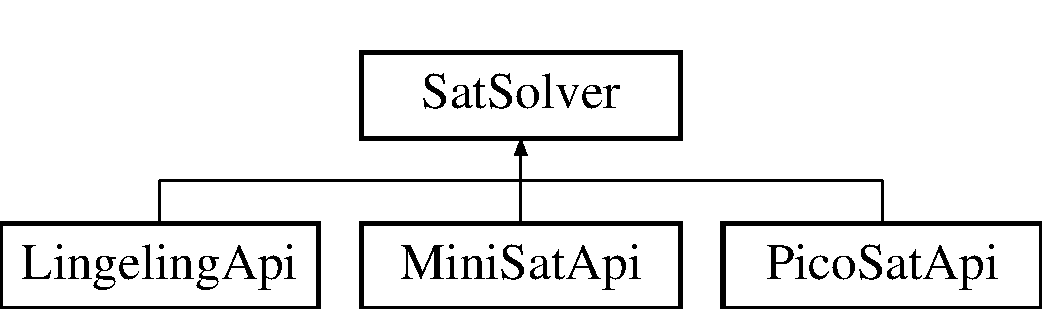
\includegraphics[height=2.000000cm]{classSatSolver}
\end{center}
\end{figure}
\subsection*{Public Member Functions}
\begin{DoxyCompactItemize}
\item 
\hyperlink{classSatSolver_a2abb0a2a75d1c3559946956ac19dc89e}{Sat\-Solver} (bool rand\-\_\-models=false, bool min\-\_\-cores=true)
\begin{DoxyCompactList}\small\item\em Constructor. \end{DoxyCompactList}\item 
virtual \hyperlink{classSatSolver_aeefe936d75dbdca120805d650a12e989}{$\sim$\-Sat\-Solver} ()
\begin{DoxyCompactList}\small\item\em Destructor. \end{DoxyCompactList}\item 
void \hyperlink{classSatSolver_a159fc9658709e5aeba2844a09454b2cb}{do\-Min\-Cores} (bool min\-\_\-cores=true)
\begin{DoxyCompactList}\small\item\em Enables or disables the computation of M\-I\-N\-I\-M\-A\-L unsatisfiable cores. \end{DoxyCompactList}\item 
void \hyperlink{classSatSolver_ae229c5e277350710412fce0e867dc566}{do\-Rand\-Models} (bool rand\-\_\-models=true)
\begin{DoxyCompactList}\small\item\em Enables or disables the randomization of satisfying assignments. \end{DoxyCompactList}\item 
virtual bool \hyperlink{classSatSolver_a82f60f60db464fbe5c66a20ad673a573}{is\-Sat} (const \hyperlink{classCNF}{C\-N\-F} \&cnf)=0
\begin{DoxyCompactList}\small\item\em Checks if a \hyperlink{classCNF}{C\-N\-F} is satisfiable. \end{DoxyCompactList}\item 
virtual bool \hyperlink{classSatSolver_ad5cfce08969be5aaf5cd705c12c68818}{is\-Sat\-Model\-Or\-Core} (const \hyperlink{classCNF}{C\-N\-F} \&cnf, const vector$<$ int $>$ \&assumptions, const vector$<$ int $>$ \&vars\-\_\-of\-\_\-interest, vector$<$ int $>$ \&model\-\_\-or\-\_\-core)=0
\begin{DoxyCompactList}\small\item\em Checks if a \hyperlink{classCNF}{C\-N\-F} is satisfiable and extracts a model or an unsatisfiable core. \end{DoxyCompactList}\item 
virtual void \hyperlink{classSatSolver_a74603f84c3f2383a5fc44d5a8093cbea}{start\-Incremental\-Session} (const vector$<$ int $>$ \&vars\-\_\-to\-\_\-keep, bool use\-\_\-push=true)=0
\begin{DoxyCompactList}\small\item\em Starts a new incremental session. \end{DoxyCompactList}\item 
virtual void \hyperlink{classSatSolver_a8118d2900f7acf31497cd2a27ad3b713}{clear\-Incremental\-Session} ()=0
\begin{DoxyCompactList}\small\item\em Deletes the solver instance that is used in the incremental session. \end{DoxyCompactList}\item 
virtual void \hyperlink{classSatSolver_ab2581b192cb2c39a81a416a9f7416c9e}{inc\-Add\-C\-N\-F} (const \hyperlink{classCNF}{C\-N\-F} \&cnf)=0
\begin{DoxyCompactList}\small\item\em Adds a new \hyperlink{classCNF}{C\-N\-F} to the current incremental session. \end{DoxyCompactList}\item 
virtual void \hyperlink{classSatSolver_a9f91c104238b6e091513e0aa46970840}{inc\-Add\-Clause} (const vector$<$ int $>$ \&clause)=0
\begin{DoxyCompactList}\small\item\em Adds a new clause to the current incremental session. \end{DoxyCompactList}\item 
virtual void \hyperlink{classSatSolver_a5b39c45cd2a1abfe96c681515dfddb77}{inc\-Add\-Unit\-Clause} (int lit)=0
\begin{DoxyCompactList}\small\item\em Adds a new unit clause to the current incremental session. \end{DoxyCompactList}\item 
virtual void \hyperlink{classSatSolver_a791be541b59ef58a29a1c517fca943e7}{inc\-Add2\-Lit\-Clause} (int lit1, int lit2)=0
\begin{DoxyCompactList}\small\item\em Adds a new clause consisting of 2 literals to the current incremental session. \end{DoxyCompactList}\item 
virtual void \hyperlink{classSatSolver_abca288874a1b8ab1a90cb274eb885ace}{inc\-Add3\-Lit\-Clause} (int lit1, int lit2, int lit3)=0
\begin{DoxyCompactList}\small\item\em Adds a new clause consisting of 3 literals to the current incremental session. \end{DoxyCompactList}\item 
virtual void \hyperlink{classSatSolver_a1f04f34bb04174489ed18d0b62241004}{inc\-Add\-Cube} (const vector$<$ int $>$ \&cube)=0
\begin{DoxyCompactList}\small\item\em Adds a new cube to the current incremental session. \end{DoxyCompactList}\item 
virtual void \hyperlink{classSatSolver_a6be2c564289a59057c4c6728a3aa9c2b}{inc\-Add\-Neg\-Cube\-As\-Clause} (const vector$<$ int $>$ \&cube)=0
\begin{DoxyCompactList}\small\item\em Adds the negation of a given cube (which is a clause) to the incremental session. \end{DoxyCompactList}\item 
virtual bool \hyperlink{classSatSolver_ab1aab4b96a36b2003450067a3799ae23}{inc\-Is\-Sat} ()=0
\begin{DoxyCompactList}\small\item\em Checks if a the \hyperlink{classCNF}{C\-N\-F} in the incremental session is satisfiable. \end{DoxyCompactList}\item 
virtual bool \hyperlink{classSatSolver_a1864787a33621efac7fc75fb6b25f080}{inc\-Is\-Sat} (const vector$<$ int $>$ \&assumptions)=0
\begin{DoxyCompactList}\small\item\em Checks if a the \hyperlink{classCNF}{C\-N\-F} in the incremental session is satisfiable under assumptions. \end{DoxyCompactList}\item 
virtual bool \hyperlink{classSatSolver_ad387fc06bacf2d48847f779c9db8461a}{inc\-Is\-Sat\-Model\-Or\-Core} (const vector$<$ int $>$ \&assumptions, const vector$<$ int $>$ \&vars\-\_\-of\-\_\-interest, vector$<$ int $>$ \&model\-\_\-or\-\_\-core)=0
\begin{DoxyCompactList}\small\item\em Checks the \hyperlink{classCNF}{C\-N\-F} in the incremental session and computes a model or unsat core. \end{DoxyCompactList}\item 
virtual bool \hyperlink{classSatSolver_a29225bfab1f352cae27c68e9bda4d409}{inc\-Is\-Sat\-Model\-Or\-Core} (const vector$<$ int $>$ \&core\-\_\-assumptions, const vector$<$ int $>$ \&more\-\_\-assumptions, const vector$<$ int $>$ \&vars\-\_\-of\-\_\-interest, vector$<$ int $>$ \&model\-\_\-or\-\_\-core)=0
\begin{DoxyCompactList}\small\item\em Computes a satisfying assignment or core using additional assumptions. \end{DoxyCompactList}\item 
virtual void \hyperlink{classSatSolver_a4da0dff7082a91429e3311d279605be4}{inc\-Push} ()=0
\begin{DoxyCompactList}\small\item\em Stores the current state of the incremental session on a stack. \end{DoxyCompactList}\item 
virtual void \hyperlink{classSatSolver_a436aae045eb04141c834df0b55947ee5}{inc\-Pop} ()=0
\begin{DoxyCompactList}\small\item\em Restores the incremental session back to the point where \hyperlink{classSatSolver_a4da0dff7082a91429e3311d279605be4}{inc\-Push()} was called. \end{DoxyCompactList}\end{DoxyCompactItemize}
\subsection*{Protected Attributes}
\begin{DoxyCompactItemize}
\item 
bool \hyperlink{classSatSolver_adfeecebfd09606c82b5c57cfe5aad813}{min\-\_\-cores\-\_\-}
\begin{DoxyCompactList}\small\item\em Indicates if the unsat cores returned by the solver should be minimized further. \end{DoxyCompactList}\item 
bool \hyperlink{classSatSolver_a73fed24d8fb4da85ef82dc53ac5f28c7}{rand\-\_\-models\-\_\-}
\begin{DoxyCompactList}\small\item\em Indicates if satisfying assignments should be randomized. \end{DoxyCompactList}\end{DoxyCompactItemize}
\subsection*{Private Member Functions}
\begin{DoxyCompactItemize}
\item 
\hyperlink{classSatSolver_a0821aa3a3fababd9b070f758b6e788cc}{Sat\-Solver} (const \hyperlink{classSatSolver}{Sat\-Solver} \&other)
\begin{DoxyCompactList}\small\item\em Copy constructor. \end{DoxyCompactList}\item 
\hyperlink{classSatSolver}{Sat\-Solver} \& \hyperlink{classSatSolver_a9dc824ecbeaf4f0505403b284f6fe047}{operator=} (const \hyperlink{classSatSolver}{Sat\-Solver} \&other)
\begin{DoxyCompactList}\small\item\em Assignment operator. \end{DoxyCompactList}\end{DoxyCompactItemize}


\subsection{Detailed Description}
An abstract interface for all S\-A\-T-\/solver implementations. 

This class represents an abstract interface all S\-A\-T-\/solver instances. You cannot instantiate objects of this class. You need to instantiate objects of one of the derived classes (e.\-g., \hyperlink{classLingelingApi}{Lingeling\-Api}, \hyperlink{classMiniSatApi}{Mini\-Sat\-Api}, \hyperlink{classPicoSatApi}{Pico\-Sat\-Api}) instead. Typically, you will call \hyperlink{classOptions_aed3731b7c89433cd485cff35ca4bdcd7}{Options\-::get\-S\-A\-T\-Solver()} to get a concrete instance of a \hyperlink{classSatSolver}{Sat\-Solver} (namely the one the user selected with command-\/line parameters).

For a given \hyperlink{classCNF}{C\-N\-F}, a \hyperlink{classSatSolver}{Sat\-Solver} is able to determine satisfiability. Furthermore, in case of satisfiability, it can extract satisfying assignments. In case of unsatisfiability, it can compute an unsatisfiable core. It can be used in two different ways. In the incremental usage scenario, all information the solver has learned so far is retained. Methods for incremental solving start with 'inc'. Other methods (like \hyperlink{classSatSolver_a82f60f60db464fbe5c66a20ad673a573}{is\-Sat()} or \hyperlink{classSatSolver_ad5cfce08969be5aaf5cd705c12c68818}{is\-Sat\-Model\-Or\-Core()}) instantiate a fresh solver instance for every call.

\begin{DoxyAuthor}{Author}
Robert Koenighofer (\href{mailto:robert.koenighofer@iaik.tugraz.at}{\tt robert.\-koenighofer@iaik.\-tugraz.\-at}) 
\end{DoxyAuthor}
\begin{DoxyVersion}{Version}
1.\-0.\-0 
\end{DoxyVersion}


Definition at line 58 of file Sat\-Solver.\-h.



\subsection{Constructor \& Destructor Documentation}
\hypertarget{classSatSolver_a2abb0a2a75d1c3559946956ac19dc89e}{\index{Sat\-Solver@{Sat\-Solver}!Sat\-Solver@{Sat\-Solver}}
\index{Sat\-Solver@{Sat\-Solver}!SatSolver@{Sat\-Solver}}
\subsubsection[{Sat\-Solver}]{\setlength{\rightskip}{0pt plus 5cm}Sat\-Solver\-::\-Sat\-Solver (
\begin{DoxyParamCaption}
\item[{bool}]{rand\-\_\-models = {\ttfamily false}, }
\item[{bool}]{min\-\_\-cores = {\ttfamily true}}
\end{DoxyParamCaption}
)}}\label{classSatSolver_a2abb0a2a75d1c3559946956ac19dc89e}


Constructor. 


\begin{DoxyParams}{Parameters}
{\em rand\-\_\-models} & A flag indicating if satisfying assignments should be randomized. This is done in a post-\/processing step (values are flipped randomly and then we check if this still constitutes a satisfying assignment). This is expensive. If this parameter is skipped, then satisfying assignments are not randomized. \\
\hline
{\em min\-\_\-cores} & A flag indicating if unsatisfiable cores returned by the solver should be minimized further by trying to drop one literal after the other. This makes the calls slower but produces potentially smaller cubes. \\
\hline
\end{DoxyParams}


Definition at line 33 of file Sat\-Solver.\-cpp.

\hypertarget{classSatSolver_aeefe936d75dbdca120805d650a12e989}{\index{Sat\-Solver@{Sat\-Solver}!$\sim$\-Sat\-Solver@{$\sim$\-Sat\-Solver}}
\index{$\sim$\-Sat\-Solver@{$\sim$\-Sat\-Solver}!SatSolver@{Sat\-Solver}}
\subsubsection[{$\sim$\-Sat\-Solver}]{\setlength{\rightskip}{0pt plus 5cm}Sat\-Solver\-::$\sim$\-Sat\-Solver (
\begin{DoxyParamCaption}
{}
\end{DoxyParamCaption}
)\hspace{0.3cm}{\ttfamily [virtual]}}}\label{classSatSolver_aeefe936d75dbdca120805d650a12e989}


Destructor. 



Definition at line 41 of file Sat\-Solver.\-cpp.

\hypertarget{classSatSolver_a0821aa3a3fababd9b070f758b6e788cc}{\index{Sat\-Solver@{Sat\-Solver}!Sat\-Solver@{Sat\-Solver}}
\index{Sat\-Solver@{Sat\-Solver}!SatSolver@{Sat\-Solver}}
\subsubsection[{Sat\-Solver}]{\setlength{\rightskip}{0pt plus 5cm}Sat\-Solver\-::\-Sat\-Solver (
\begin{DoxyParamCaption}
\item[{const {\bf Sat\-Solver} \&}]{other}
\end{DoxyParamCaption}
)\hspace{0.3cm}{\ttfamily [private]}}}\label{classSatSolver_a0821aa3a3fababd9b070f758b6e788cc}


Copy constructor. 

The copy constructor is disabled (set private) and not implemented.


\begin{DoxyParams}{Parameters}
{\em other} & The source for creating the copy. \\
\hline
\end{DoxyParams}


\subsection{Member Function Documentation}
\hypertarget{classSatSolver_a8118d2900f7acf31497cd2a27ad3b713}{\index{Sat\-Solver@{Sat\-Solver}!clear\-Incremental\-Session@{clear\-Incremental\-Session}}
\index{clear\-Incremental\-Session@{clear\-Incremental\-Session}!SatSolver@{Sat\-Solver}}
\subsubsection[{clear\-Incremental\-Session}]{\setlength{\rightskip}{0pt plus 5cm}virtual void Sat\-Solver\-::clear\-Incremental\-Session (
\begin{DoxyParamCaption}
{}
\end{DoxyParamCaption}
)\hspace{0.3cm}{\ttfamily [pure virtual]}}}\label{classSatSolver_a8118d2900f7acf31497cd2a27ad3b713}


Deletes the solver instance that is used in the incremental session. 



Implemented in \hyperlink{classMiniSatApi_a237754c78357ed0a84894e811806b618}{Mini\-Sat\-Api}, \hyperlink{classPicoSatApi_ae53598723725fd3203e2e32411392dab}{Pico\-Sat\-Api}, and \hyperlink{classLingelingApi_a4200b2ca7b1694898434ae9764f5baf6}{Lingeling\-Api}.

\hypertarget{classSatSolver_a159fc9658709e5aeba2844a09454b2cb}{\index{Sat\-Solver@{Sat\-Solver}!do\-Min\-Cores@{do\-Min\-Cores}}
\index{do\-Min\-Cores@{do\-Min\-Cores}!SatSolver@{Sat\-Solver}}
\subsubsection[{do\-Min\-Cores}]{\setlength{\rightskip}{0pt plus 5cm}void Sat\-Solver\-::do\-Min\-Cores (
\begin{DoxyParamCaption}
\item[{bool}]{min\-\_\-cores = {\ttfamily true}}
\end{DoxyParamCaption}
)}}\label{classSatSolver_a159fc9658709e5aeba2844a09454b2cb}


Enables or disables the computation of M\-I\-N\-I\-M\-A\-L unsatisfiable cores. 


\begin{DoxyParams}{Parameters}
{\em min\-\_\-cores} & A flag indicating if unsatisfiable cores returned by the solver should be minimized further by trying to drop one literal after the other. This makes the calls slower but produces potentially smaller cubes. If the parameter is skipped the computation of minimal cores is enabled. \\
\hline
\end{DoxyParams}


Definition at line 47 of file Sat\-Solver.\-cpp.



References min\-\_\-cores\-\_\-.



Referenced by Learn\-Synth\-S\-A\-T\-::compute\-Winning\-Region\-Plain(), Learn\-Synth\-S\-A\-T\-::compute\-Winning\-Region\-R\-G(), and Learn\-Synth\-S\-A\-T\-::compute\-Winning\-Region\-R\-G\-R\-C().

\hypertarget{classSatSolver_ae229c5e277350710412fce0e867dc566}{\index{Sat\-Solver@{Sat\-Solver}!do\-Rand\-Models@{do\-Rand\-Models}}
\index{do\-Rand\-Models@{do\-Rand\-Models}!SatSolver@{Sat\-Solver}}
\subsubsection[{do\-Rand\-Models}]{\setlength{\rightskip}{0pt plus 5cm}void Sat\-Solver\-::do\-Rand\-Models (
\begin{DoxyParamCaption}
\item[{bool}]{rand\-\_\-models = {\ttfamily true}}
\end{DoxyParamCaption}
)}}\label{classSatSolver_ae229c5e277350710412fce0e867dc566}


Enables or disables the randomization of satisfying assignments. 


\begin{DoxyParams}{Parameters}
{\em rand\-\_\-models} & A flag indicating if satisfying assignments should be randomized. This is done in a post-\/processing step (values are flipped randomly and then we check if this still constitutes a satisfying assignment). This is expensive. If this parameter is skipped, then randomization is enabled. \\
\hline
\end{DoxyParams}


Definition at line 53 of file Sat\-Solver.\-cpp.



References rand\-\_\-models\-\_\-.



Referenced by Learn\-Synth\-S\-A\-T\-::compute\-Winning\-Region\-Plain(), Learn\-Synth\-S\-A\-T\-::compute\-Winning\-Region\-R\-G(), and Learn\-Synth\-S\-A\-T\-::compute\-Winning\-Region\-R\-G\-R\-C().

\hypertarget{classSatSolver_a791be541b59ef58a29a1c517fca943e7}{\index{Sat\-Solver@{Sat\-Solver}!inc\-Add2\-Lit\-Clause@{inc\-Add2\-Lit\-Clause}}
\index{inc\-Add2\-Lit\-Clause@{inc\-Add2\-Lit\-Clause}!SatSolver@{Sat\-Solver}}
\subsubsection[{inc\-Add2\-Lit\-Clause}]{\setlength{\rightskip}{0pt plus 5cm}virtual void Sat\-Solver\-::inc\-Add2\-Lit\-Clause (
\begin{DoxyParamCaption}
\item[{int}]{lit1, }
\item[{int}]{lit2}
\end{DoxyParamCaption}
)\hspace{0.3cm}{\ttfamily [pure virtual]}}}\label{classSatSolver_a791be541b59ef58a29a1c517fca943e7}


Adds a new clause consisting of 2 literals to the current incremental session. 

This is an abstract method which must be implemented in all derived classes (all classes implementing this interface).

\begin{DoxyPrecond}{Precondition}
\hyperlink{classSatSolver_a74603f84c3f2383a5fc44d5a8093cbea}{start\-Incremental\-Session()} must have been called before. 
\end{DoxyPrecond}

\begin{DoxyParams}{Parameters}
{\em lit1} & The first literal of the clause to add to the currently open incremental session. If this method is called after solving for the first time, be sure that the passed literal talks about a variables that have been mentioned in vars\-\_\-to\-\_\-keep when calling \hyperlink{classSatSolver_a74603f84c3f2383a5fc44d5a8093cbea}{start\-Incremental\-Session()}. \\
\hline
{\em lit2} & The second literal of the clause to add to the currently open incremental session (must be contained in vars\-\_\-to\-\_\-keep as well). \\
\hline
\end{DoxyParams}


Implemented in \hyperlink{classMiniSatApi_a56c4758ee7466cd7fa48a682fee76fd3}{Mini\-Sat\-Api}, \hyperlink{classPicoSatApi_a5c31301a2b0dfc70251f285e737a6fc2}{Pico\-Sat\-Api}, and \hyperlink{classLingelingApi_a54bf3198e6bb2dd3ebda768272337955}{Lingeling\-Api}.

\hypertarget{classSatSolver_abca288874a1b8ab1a90cb274eb885ace}{\index{Sat\-Solver@{Sat\-Solver}!inc\-Add3\-Lit\-Clause@{inc\-Add3\-Lit\-Clause}}
\index{inc\-Add3\-Lit\-Clause@{inc\-Add3\-Lit\-Clause}!SatSolver@{Sat\-Solver}}
\subsubsection[{inc\-Add3\-Lit\-Clause}]{\setlength{\rightskip}{0pt plus 5cm}virtual void Sat\-Solver\-::inc\-Add3\-Lit\-Clause (
\begin{DoxyParamCaption}
\item[{int}]{lit1, }
\item[{int}]{lit2, }
\item[{int}]{lit3}
\end{DoxyParamCaption}
)\hspace{0.3cm}{\ttfamily [pure virtual]}}}\label{classSatSolver_abca288874a1b8ab1a90cb274eb885ace}


Adds a new clause consisting of 3 literals to the current incremental session. 

This is an abstract method which must be implemented in all derived classes (all classes implementing this interface).

\begin{DoxyPrecond}{Precondition}
\hyperlink{classSatSolver_a74603f84c3f2383a5fc44d5a8093cbea}{start\-Incremental\-Session()} must have been called before. 
\end{DoxyPrecond}

\begin{DoxyParams}{Parameters}
{\em lit1} & The first literal of the clause to add to the currently open incremental session. If this method is called after solving for the first time, be sure that the passed literal talks about a variables that have been mentioned in vars\-\_\-to\-\_\-keep when calling \hyperlink{classSatSolver_a74603f84c3f2383a5fc44d5a8093cbea}{start\-Incremental\-Session()}. \\
\hline
{\em lit2} & The second literal of the clause to add to the currently open incremental session (must be contained in vars\-\_\-to\-\_\-keep as well). \\
\hline
{\em lit3} & The third literal of the clause to add to the currently open incremental session (must be contained in vars\-\_\-to\-\_\-keep as well). \\
\hline
\end{DoxyParams}


Implemented in \hyperlink{classMiniSatApi_aee9556c8c5de695fa5d7aa7cfde57877}{Mini\-Sat\-Api}, \hyperlink{classPicoSatApi_a1daeb6e2b3bfa3eee44a7bf1b278dd86}{Pico\-Sat\-Api}, and \hyperlink{classLingelingApi_ad05f795bbf472fe5386164a74a8ecd86}{Lingeling\-Api}.

\hypertarget{classSatSolver_a9f91c104238b6e091513e0aa46970840}{\index{Sat\-Solver@{Sat\-Solver}!inc\-Add\-Clause@{inc\-Add\-Clause}}
\index{inc\-Add\-Clause@{inc\-Add\-Clause}!SatSolver@{Sat\-Solver}}
\subsubsection[{inc\-Add\-Clause}]{\setlength{\rightskip}{0pt plus 5cm}virtual void Sat\-Solver\-::inc\-Add\-Clause (
\begin{DoxyParamCaption}
\item[{const vector$<$ int $>$ \&}]{clause}
\end{DoxyParamCaption}
)\hspace{0.3cm}{\ttfamily [pure virtual]}}}\label{classSatSolver_a9f91c104238b6e091513e0aa46970840}


Adds a new clause to the current incremental session. 

This is an abstract method which must be implemented in all derived classes (all classes implementing this interface).

\begin{DoxyPrecond}{Precondition}
\hyperlink{classSatSolver_a74603f84c3f2383a5fc44d5a8093cbea}{start\-Incremental\-Session()} must have been called before. 
\end{DoxyPrecond}

\begin{DoxyParams}{Parameters}
{\em clause} & The clause (a disjunction of literals) to add (conjunct) to the currently open incremental session. If this method is called after solving for the first time, be sure that the passed clause talks only about variables that have been mentioned in vars\-\_\-to\-\_\-keep when calling \hyperlink{classSatSolver_a74603f84c3f2383a5fc44d5a8093cbea}{start\-Incremental\-Session()}. \\
\hline
\end{DoxyParams}


Implemented in \hyperlink{classMiniSatApi_af2115a84419b7480ff55b747f7ddd60a}{Mini\-Sat\-Api}, \hyperlink{classPicoSatApi_aaafa1c5c7f1058029127a39a32ceada6}{Pico\-Sat\-Api}, and \hyperlink{classLingelingApi_afb3e0d0ab541b89ef6c281145f53105f}{Lingeling\-Api}.



Referenced by I\-F\-M13\-Synth\-::add\-Blocked\-State(), I\-F\-M13\-Explorer\-::add\-Blocked\-State(), I\-F\-M13\-Synth\-::add\-Blocked\-Transition(), I\-F\-M13\-Explorer\-::add\-Blocked\-Transition(), I\-F\-M13\-Synth\-::add\-Lose(), Utils\-::compress\-State\-C\-N\-F(), Learn\-Synth\-Q\-B\-F\-::compute\-Counterexample\-S\-A\-T(), Learn\-Synth\-Q\-B\-F\-::compute\-Winning\-Region\-One\-S\-A\-T(), Learn\-Synth\-S\-A\-T\-::compute\-Winning\-Region\-Plain(), Learn\-Synth\-S\-A\-T\-::compute\-Winning\-Region\-R\-G(), Learn\-Synth\-S\-A\-T\-::compute\-Winning\-Region\-R\-G\-R\-C(), I\-F\-M13\-Synth\-::propagate\-Blocked\-States(), and I\-F\-M13\-Explorer\-::propagate\-Blocked\-States().

\hypertarget{classSatSolver_ab2581b192cb2c39a81a416a9f7416c9e}{\index{Sat\-Solver@{Sat\-Solver}!inc\-Add\-C\-N\-F@{inc\-Add\-C\-N\-F}}
\index{inc\-Add\-C\-N\-F@{inc\-Add\-C\-N\-F}!SatSolver@{Sat\-Solver}}
\subsubsection[{inc\-Add\-C\-N\-F}]{\setlength{\rightskip}{0pt plus 5cm}virtual void Sat\-Solver\-::inc\-Add\-C\-N\-F (
\begin{DoxyParamCaption}
\item[{const {\bf C\-N\-F} \&}]{cnf}
\end{DoxyParamCaption}
)\hspace{0.3cm}{\ttfamily [pure virtual]}}}\label{classSatSolver_ab2581b192cb2c39a81a416a9f7416c9e}


Adds a new \hyperlink{classCNF}{C\-N\-F} to the current incremental session. 

This is an abstract method which must be implemented in all derived classes (all classes implementing this interface).

\begin{DoxyPrecond}{Precondition}
\hyperlink{classSatSolver_a74603f84c3f2383a5fc44d5a8093cbea}{start\-Incremental\-Session()} must have been called before. 
\end{DoxyPrecond}

\begin{DoxyParams}{Parameters}
{\em cnf} & The \hyperlink{classCNF}{C\-N\-F} to add to the currently open incremental session. If this method is called after solving for the first time, be sure that the passed \hyperlink{classCNF}{C\-N\-F} talks only about variables that have been mentioned in vars\-\_\-to\-\_\-keep when calling \hyperlink{classSatSolver_a74603f84c3f2383a5fc44d5a8093cbea}{start\-Incremental\-Session()}. \\
\hline
\end{DoxyParams}


Implemented in \hyperlink{classMiniSatApi_ae5ffe2811e01051c5206c9e4865a7102}{Mini\-Sat\-Api}, \hyperlink{classPicoSatApi_a619b3cb3b059b06c34f84d9ae123c042}{Pico\-Sat\-Api}, and \hyperlink{classLingelingApi_ae9e54e64007c98add90e142a5c38d4bc}{Lingeling\-Api}.



Referenced by Counter\-Gen\-S\-A\-T\-::compress\-Bored(), Utils\-::compress\-State\-C\-N\-F(), Learn\-Synth\-Q\-B\-F\-::compute\-Counterexample\-S\-A\-T(), Learn\-Synth\-S\-A\-T\-::compute\-Winning\-Region\-Plain(), Learn\-Synth\-S\-A\-T\-::compute\-Winning\-Region\-R\-G(), Learn\-Synth\-S\-A\-T\-::compute\-Winning\-Region\-R\-G\-R\-C(), Clause\-Explorer\-S\-A\-T\-::consider\-New\-Info\-From\-Others(), Counter\-Gen\-S\-A\-T\-::consider\-New\-Info\-From\-Others(), I\-F\-M13\-Explorer\-::consider\-New\-Info\-From\-Others(), Clause\-Explorer\-S\-A\-T\-::explore\-Clauses(), Counter\-Gen\-S\-A\-T\-::generalize\-Counterexamples(), I\-F\-M13\-Explorer\-::\-I\-F\-M13\-Explorer(), I\-F\-M13\-Synth\-::\-I\-F\-M13\-Synth(), and Learn\-Synth\-Q\-B\-F\-::\-Learn\-Synth\-Q\-B\-F().

\hypertarget{classSatSolver_a1f04f34bb04174489ed18d0b62241004}{\index{Sat\-Solver@{Sat\-Solver}!inc\-Add\-Cube@{inc\-Add\-Cube}}
\index{inc\-Add\-Cube@{inc\-Add\-Cube}!SatSolver@{Sat\-Solver}}
\subsubsection[{inc\-Add\-Cube}]{\setlength{\rightskip}{0pt plus 5cm}virtual void Sat\-Solver\-::inc\-Add\-Cube (
\begin{DoxyParamCaption}
\item[{const vector$<$ int $>$ \&}]{cube}
\end{DoxyParamCaption}
)\hspace{0.3cm}{\ttfamily [pure virtual]}}}\label{classSatSolver_a1f04f34bb04174489ed18d0b62241004}


Adds a new cube to the current incremental session. 

That is, all literals of the cube are added as unit clauses to the current incremental session. For instance, if the cube \mbox{[}2, -\/4, 8\mbox{]} is passed as argument, then this method adds the three unit clauses \mbox{[}2\mbox{]}, \mbox{[}-\/4\mbox{]}, \mbox{[}8\mbox{]}.

This is an abstract method which must be implemented in all derived classes (all classes implementing this interface).

\begin{DoxyPrecond}{Precondition}
\hyperlink{classSatSolver_a74603f84c3f2383a5fc44d5a8093cbea}{start\-Incremental\-Session()} must have been called before. 
\end{DoxyPrecond}

\begin{DoxyParams}{Parameters}
{\em cube} & The cube (a conjunction of literals) to add (conjunct) to the currently open incremental session. All literals of this cube will be added as unit clauses. If this method is called after solving for the first time, be sure that the passed clause talks only about variables that have been mentioned in vars\-\_\-to\-\_\-keep when calling \hyperlink{classSatSolver_a74603f84c3f2383a5fc44d5a8093cbea}{start\-Incremental\-Session()}. \\
\hline
\end{DoxyParams}


Implemented in \hyperlink{classMiniSatApi_a41e16a2e8757846fa17e010c5cc1ff16}{Mini\-Sat\-Api}, \hyperlink{classPicoSatApi_ae0a7dd7da9ead164560f454e29457453}{Pico\-Sat\-Api}, and \hyperlink{classLingelingApi_a6dc0eb0582d6afda381fc05a5820433c}{Lingeling\-Api}.



Referenced by Learn\-Synth\-S\-A\-T\-::compute\-Winning\-Region\-R\-G(), Learn\-Synth\-S\-A\-T\-::compute\-Winning\-Region\-R\-G\-R\-C(), Clause\-Explorer\-S\-A\-T\-::explore\-Clauses(), and Counter\-Gen\-S\-A\-T\-::generalize\-Ce\-Futher().

\hypertarget{classSatSolver_a6be2c564289a59057c4c6728a3aa9c2b}{\index{Sat\-Solver@{Sat\-Solver}!inc\-Add\-Neg\-Cube\-As\-Clause@{inc\-Add\-Neg\-Cube\-As\-Clause}}
\index{inc\-Add\-Neg\-Cube\-As\-Clause@{inc\-Add\-Neg\-Cube\-As\-Clause}!SatSolver@{Sat\-Solver}}
\subsubsection[{inc\-Add\-Neg\-Cube\-As\-Clause}]{\setlength{\rightskip}{0pt plus 5cm}virtual void Sat\-Solver\-::inc\-Add\-Neg\-Cube\-As\-Clause (
\begin{DoxyParamCaption}
\item[{const vector$<$ int $>$ \&}]{cube}
\end{DoxyParamCaption}
)\hspace{0.3cm}{\ttfamily [pure virtual]}}}\label{classSatSolver_a6be2c564289a59057c4c6728a3aa9c2b}


Adds the negation of a given cube (which is a clause) to the incremental session. 

For instance, if the cube \mbox{[}2, -\/4, 8\mbox{]} is passed as argument, then this method adds the clauses \mbox{[}-\/2, 4, -\/8\mbox{]} to the current incremental session.

This is an abstract method which must be implemented in all derived classes (all classes implementing this interface).

\begin{DoxyPrecond}{Precondition}
\hyperlink{classSatSolver_a74603f84c3f2383a5fc44d5a8093cbea}{start\-Incremental\-Session()} must have been called before. 
\end{DoxyPrecond}

\begin{DoxyParams}{Parameters}
{\em cube} & The cube (a conjunction of literals) to negate and add (conjunct) to the currently open incremental session. If this method is called after solving for the first time, be sure that the passed cube talks only about variables that have been mentioned in vars\-\_\-to\-\_\-keep when calling \hyperlink{classSatSolver_a74603f84c3f2383a5fc44d5a8093cbea}{start\-Incremental\-Session()}. \\
\hline
\end{DoxyParams}


Implemented in \hyperlink{classMiniSatApi_a49afe5c41bb036a31f65f98621e82846}{Mini\-Sat\-Api}, \hyperlink{classPicoSatApi_ace9bfbd0c8cbd62c3e92d2b208bb7b66}{Pico\-Sat\-Api}, and \hyperlink{classLingelingApi_afefd24f97e49aed7cbaf25140a6b7741}{Lingeling\-Api}.



Referenced by Counter\-Gen\-S\-A\-T\-::compress\-Bored(), Learn\-Synth\-S\-A\-T\-::compute\-Winning\-Region\-R\-G(), Learn\-Synth\-S\-A\-T\-::compute\-Winning\-Region\-R\-G\-R\-C(), Clause\-Explorer\-S\-A\-T\-::explore\-Clauses(), and Counter\-Gen\-S\-A\-T\-::generalize\-Ce\-Futher().

\hypertarget{classSatSolver_a5b39c45cd2a1abfe96c681515dfddb77}{\index{Sat\-Solver@{Sat\-Solver}!inc\-Add\-Unit\-Clause@{inc\-Add\-Unit\-Clause}}
\index{inc\-Add\-Unit\-Clause@{inc\-Add\-Unit\-Clause}!SatSolver@{Sat\-Solver}}
\subsubsection[{inc\-Add\-Unit\-Clause}]{\setlength{\rightskip}{0pt plus 5cm}virtual void Sat\-Solver\-::inc\-Add\-Unit\-Clause (
\begin{DoxyParamCaption}
\item[{int}]{lit}
\end{DoxyParamCaption}
)\hspace{0.3cm}{\ttfamily [pure virtual]}}}\label{classSatSolver_a5b39c45cd2a1abfe96c681515dfddb77}


Adds a new unit clause to the current incremental session. 

This is an abstract method which must be implemented in all derived classes (all classes implementing this interface).

\begin{DoxyPrecond}{Precondition}
\hyperlink{classSatSolver_a74603f84c3f2383a5fc44d5a8093cbea}{start\-Incremental\-Session()} must have been called before. 
\end{DoxyPrecond}

\begin{DoxyParams}{Parameters}
{\em lit} & The (one and only) literal of the unit clause to add to the currently open incremental session. If this method is called after solving for the first time, be sure that the passed literal talks about a variables that have been mentioned in vars\-\_\-to\-\_\-keep when calling \hyperlink{classSatSolver_a74603f84c3f2383a5fc44d5a8093cbea}{start\-Incremental\-Session()}. \\
\hline
\end{DoxyParams}


Implemented in \hyperlink{classMiniSatApi_ade09bb38667bb23f2ac993e2d6c66408}{Mini\-Sat\-Api}, \hyperlink{classPicoSatApi_a0ef01830dacfd23f63928b44ff3df788}{Pico\-Sat\-Api}, and \hyperlink{classLingelingApi_aa5c928ad16d2dc79d42b977237d377e0}{Lingeling\-Api}.



Referenced by Learn\-Synth\-S\-A\-T\-::compute\-Winning\-Region\-R\-G(), Learn\-Synth\-S\-A\-T\-::compute\-Winning\-Region\-R\-G\-R\-C(), Clause\-Explorer\-S\-A\-T\-::explore\-Clauses(), and Counter\-Gen\-S\-A\-T\-::generalize\-Counterexamples().

\hypertarget{classSatSolver_ab1aab4b96a36b2003450067a3799ae23}{\index{Sat\-Solver@{Sat\-Solver}!inc\-Is\-Sat@{inc\-Is\-Sat}}
\index{inc\-Is\-Sat@{inc\-Is\-Sat}!SatSolver@{Sat\-Solver}}
\subsubsection[{inc\-Is\-Sat}]{\setlength{\rightskip}{0pt plus 5cm}virtual bool Sat\-Solver\-::inc\-Is\-Sat (
\begin{DoxyParamCaption}
{}
\end{DoxyParamCaption}
)\hspace{0.3cm}{\ttfamily [pure virtual]}}}\label{classSatSolver_ab1aab4b96a36b2003450067a3799ae23}


Checks if a the \hyperlink{classCNF}{C\-N\-F} in the incremental session is satisfiable. 

This is an abstract method which must be implemented in all derived classes (all classes implementing this interface).

\begin{DoxyPrecond}{Precondition}
\hyperlink{classSatSolver_a74603f84c3f2383a5fc44d5a8093cbea}{start\-Incremental\-Session()} must have been called before. 
\end{DoxyPrecond}
\begin{DoxyReturn}{Returns}
True in case of satisfiability, false otherwise. 
\end{DoxyReturn}


Implemented in \hyperlink{classMiniSatApi_a4c6ba65381002eb3f90e8e0df1606759}{Mini\-Sat\-Api}, \hyperlink{classPicoSatApi_a0d1237c039315d572fb0828c59435177}{Pico\-Sat\-Api}, and \hyperlink{classLingelingApi_a7a96e3b1078e40305f8b5e329f0a1e26}{Lingeling\-Api}.



Referenced by I\-F\-M13\-Synth\-::add\-Blocked\-State(), I\-F\-M13\-Explorer\-::add\-Blocked\-State(), Counter\-Gen\-S\-A\-T\-::bored(), Counter\-Gen\-S\-A\-T\-::compress\-Bored(), Utils\-::compress\-State\-C\-N\-F(), Learn\-Synth\-S\-A\-T\-::compute\-Winning\-Region\-R\-G(), Learn\-Synth\-S\-A\-T\-::compute\-Winning\-Region\-R\-G\-R\-C(), Clause\-Explorer\-S\-A\-T\-::explore\-Clauses(), Counter\-Gen\-S\-A\-T\-::generalize\-Ce\-Futher(), Counter\-Gen\-S\-A\-T\-::generalize\-Counterexamples(), I\-F\-M13\-Synth\-::propagate\-Blocked\-States(), and I\-F\-M13\-Explorer\-::propagate\-Blocked\-States().

\hypertarget{classSatSolver_a1864787a33621efac7fc75fb6b25f080}{\index{Sat\-Solver@{Sat\-Solver}!inc\-Is\-Sat@{inc\-Is\-Sat}}
\index{inc\-Is\-Sat@{inc\-Is\-Sat}!SatSolver@{Sat\-Solver}}
\subsubsection[{inc\-Is\-Sat}]{\setlength{\rightskip}{0pt plus 5cm}virtual bool Sat\-Solver\-::inc\-Is\-Sat (
\begin{DoxyParamCaption}
\item[{const vector$<$ int $>$ \&}]{assumptions}
\end{DoxyParamCaption}
)\hspace{0.3cm}{\ttfamily [pure virtual]}}}\label{classSatSolver_a1864787a33621efac7fc75fb6b25f080}


Checks if a the \hyperlink{classCNF}{C\-N\-F} in the incremental session is satisfiable under assumptions. 

This method checks if the \hyperlink{classCNF}{C\-N\-F} in the incremental session is satisfiable given that all literals passed in the vector 'assumptions' are true. The assumptions are not persistently added to the \hyperlink{classCNF}{C\-N\-F} of the incremental session.

This is an abstract method which must be implemented in all derived classes (all classes implementing this interface).

\begin{DoxyPrecond}{Precondition}
\hyperlink{classSatSolver_a74603f84c3f2383a5fc44d5a8093cbea}{start\-Incremental\-Session()} must have been called before. 
\end{DoxyPrecond}

\begin{DoxyParams}{Parameters}
{\em assumptions} & A vector of literals. This method then checks if the \hyperlink{classCNF}{C\-N\-F} of the incremental session is satisfiable given that all literals passed in this vector are true. The assumptions are not persistently added to the \hyperlink{classCNF}{C\-N\-F}. The assumptions must be a subset of the vars\-\_\-to\-\_\-keep passed to \hyperlink{classSatSolver_a74603f84c3f2383a5fc44d5a8093cbea}{start\-Incremental\-Session()}. \\
\hline
\end{DoxyParams}
\begin{DoxyReturn}{Returns}
True in case of satisfiability, false otherwise. 
\end{DoxyReturn}


Implemented in \hyperlink{classMiniSatApi_a40421bac2739bacb68f3c7083810694b}{Mini\-Sat\-Api}, \hyperlink{classPicoSatApi_abebe28c72303235d2fdc915bbf4752c0}{Pico\-Sat\-Api}, and \hyperlink{classLingelingApi_a192ddd0f1d27617570c759b3496ea90d}{Lingeling\-Api}.

\hypertarget{classSatSolver_ad387fc06bacf2d48847f779c9db8461a}{\index{Sat\-Solver@{Sat\-Solver}!inc\-Is\-Sat\-Model\-Or\-Core@{inc\-Is\-Sat\-Model\-Or\-Core}}
\index{inc\-Is\-Sat\-Model\-Or\-Core@{inc\-Is\-Sat\-Model\-Or\-Core}!SatSolver@{Sat\-Solver}}
\subsubsection[{inc\-Is\-Sat\-Model\-Or\-Core}]{\setlength{\rightskip}{0pt plus 5cm}virtual bool Sat\-Solver\-::inc\-Is\-Sat\-Model\-Or\-Core (
\begin{DoxyParamCaption}
\item[{const vector$<$ int $>$ \&}]{assumptions, }
\item[{const vector$<$ int $>$ \&}]{vars\-\_\-of\-\_\-interest, }
\item[{vector$<$ int $>$ \&}]{model\-\_\-or\-\_\-core}
\end{DoxyParamCaption}
)\hspace{0.3cm}{\ttfamily [pure virtual]}}}\label{classSatSolver_ad387fc06bacf2d48847f779c9db8461a}


Checks the \hyperlink{classCNF}{C\-N\-F} in the incremental session and computes a model or unsat core. 

This method checks if the \hyperlink{classCNF}{C\-N\-F} of the incremental session is satisfiable given that all literals passed in the vector 'assumptions' is true. If this is the case, then a satisfying assignment will be written into model\-\_\-or\-\_\-core. You can specify which variables you want to have in the satisfying assignment using the vars\-\_\-of\-\_\-interest vector. The reason is that your \hyperlink{classCNF}{C\-N\-F} may contain thousands of temporary variables stemming from some Tseitin encoding, but usually one in only interested in the value of a few variables. In case of unsatisfiability, an unsatisfiable core is stored in model\-\_\-or\-\_\-core. The unsatisfiable core is a subset of the literals passed in 'assumptions' such that the \hyperlink{classCNF}{C\-N\-F} is still unsatisfiable when these literals hold.

This is an abstract method which must be implemented in all derived classes (all classes implementing this interface).


\begin{DoxyParams}{Parameters}
{\em assumptions} & A vector of literals. This method then checks if the \hyperlink{classCNF}{C\-N\-F} of the incremental session is satisfiable given that all literals passed in this vector are true. The assumptions are not persistently added to the \hyperlink{classCNF}{C\-N\-F}. The assumptions must be a subset of the vars\-\_\-to\-\_\-keep passed to \hyperlink{classSatSolver_a74603f84c3f2383a5fc44d5a8093cbea}{start\-Incremental\-Session()}. \\
\hline
{\em vars\-\_\-of\-\_\-interest} & The variables for which you want to have a value in case of satisfiability. vars\-\_\-of\-\_\-interest must be a subset of the vars\-\_\-to\-\_\-keep passed to \hyperlink{classSatSolver_a74603f84c3f2383a5fc44d5a8093cbea}{start\-Incremental\-Session()}. \\
\hline
{\em model\-\_\-or\-\_\-core} & An empty vector. Depending on the outcome of the call, either a satisfying assignment (a cube over the variables passed in vars\-\_\-of\-\_\-interest) or an unsatisfiable core (a subset of the literals passed in 'assumptions') will be written into this vector. \\
\hline
\end{DoxyParams}
\begin{DoxyReturn}{Returns}
True in case of satisfiability (of the \hyperlink{classCNF}{C\-N\-F} of the incremental session in conjunction conjuncted with all assumptions), false otherwise. 
\end{DoxyReturn}


Implemented in \hyperlink{classMiniSatApi_afb886d40bb45b5cf2fadb7aee1a06b3e}{Mini\-Sat\-Api}, \hyperlink{classPicoSatApi_aa8c0dbf4587ff4666ce20fd325364c4a}{Pico\-Sat\-Api}, and \hyperlink{classLingelingApi_a5f70806ab80cb622f4f7286f66284c4e}{Lingeling\-Api}.



Referenced by Utils\-::compress\-State\-C\-N\-F(), Learn\-Synth\-Q\-B\-F\-::compute\-Counterexample\-S\-A\-T(), Learn\-Synth\-S\-A\-T\-::compute\-Winning\-Region\-Plain(), Learn\-Synth\-S\-A\-T\-::compute\-Winning\-Region\-R\-G(), Learn\-Synth\-S\-A\-T\-::compute\-Winning\-Region\-R\-G\-R\-C(), Clause\-Explorer\-S\-A\-T\-::explore\-Clauses(), I\-F\-M13\-Synth\-::gen\-And\-Block\-Trans(), I\-F\-M13\-Explorer\-::gen\-And\-Block\-Trans(), Counter\-Gen\-S\-A\-T\-::generalize\-Ce\-Futher(), Counter\-Gen\-S\-A\-T\-::generalize\-Counterexample(), I\-F\-M13\-Synth\-::rec\-Block\-Cube(), and I\-F\-M13\-Explorer\-::rec\-Block\-Cube().

\hypertarget{classSatSolver_a29225bfab1f352cae27c68e9bda4d409}{\index{Sat\-Solver@{Sat\-Solver}!inc\-Is\-Sat\-Model\-Or\-Core@{inc\-Is\-Sat\-Model\-Or\-Core}}
\index{inc\-Is\-Sat\-Model\-Or\-Core@{inc\-Is\-Sat\-Model\-Or\-Core}!SatSolver@{Sat\-Solver}}
\subsubsection[{inc\-Is\-Sat\-Model\-Or\-Core}]{\setlength{\rightskip}{0pt plus 5cm}virtual bool Sat\-Solver\-::inc\-Is\-Sat\-Model\-Or\-Core (
\begin{DoxyParamCaption}
\item[{const vector$<$ int $>$ \&}]{core\-\_\-assumptions, }
\item[{const vector$<$ int $>$ \&}]{more\-\_\-assumptions, }
\item[{const vector$<$ int $>$ \&}]{vars\-\_\-of\-\_\-interest, }
\item[{vector$<$ int $>$ \&}]{model\-\_\-or\-\_\-core}
\end{DoxyParamCaption}
)\hspace{0.3cm}{\ttfamily [pure virtual]}}}\label{classSatSolver_a29225bfab1f352cae27c68e9bda4d409}


Computes a satisfying assignment or core using additional assumptions. 

In contrast to the previous method, this one allows to define two sets of assumptions. The core\-\_\-assumptions are used as basis for extracting an unsatisfiable core in case of unsatisfiability. The more\-\_\-assumptions are assumed but not considered for the computation of unsatisfiable cores. This is convenient to avoid calls to \hyperlink{classSatSolver_a4da0dff7082a91429e3311d279605be4}{inc\-Push()} and \hyperlink{classSatSolver_a436aae045eb04141c834df0b55947ee5}{inc\-Pop()} when temporarily working under assumptions that should not be minimized for the unsatisfiable core.

This is an abstract method which must be implemented in all derived classes (all classes implementing this interface).


\begin{DoxyParams}{Parameters}
{\em core\-\_\-assumptions} & A vector of literals. This method then checks if the \hyperlink{classCNF}{C\-N\-F} of the incremental session is satisfiable given that all literals passed in this vector and all literals passed in more\-\_\-assumptions are true. However, for computing the the unsatisfiable core, only the core\-\_\-assumptions will be minimized and the more\-\_\-assumptions stay as they are. That is, in case of unsatisfiability, model\-\_\-or\-\_\-core will contain a subset X of the core\-\_\-assumptions such that X \& more\-\_\-assumptions \& incremental\-\_\-cnf is still unsatisfiable. core\-\_\-assumptions must be a subset of the vars\-\_\-to\-\_\-keep passed to \hyperlink{classSatSolver_a74603f84c3f2383a5fc44d5a8093cbea}{start\-Incremental\-Session()}. \\
\hline
{\em more\-\_\-assumptions} & A vector of assumptions that are assumed, but not minimized when an unsatisfiable core is computed. That is, in case of unsatisfiability, model\-\_\-or\-\_\-core will contain a subset X of the core\-\_\-assumptions such that X \& more\-\_\-assumptions \& incremental\-\_\-cnf is still unsatisfiable. more\-\_\-assumptions must be a subset of the vars\-\_\-to\-\_\-keep passed to \hyperlink{classSatSolver_a74603f84c3f2383a5fc44d5a8093cbea}{start\-Incremental\-Session()}. \\
\hline
{\em vars\-\_\-of\-\_\-interest} & The variables for which you want to have a value in case of satisfiability. vars\-\_\-of\-\_\-interest must be a subset of the vars\-\_\-to\-\_\-keep passed to \hyperlink{classSatSolver_a74603f84c3f2383a5fc44d5a8093cbea}{start\-Incremental\-Session()}. \\
\hline
{\em model\-\_\-or\-\_\-core} & An empty vector. Depending on the outcome of the call, either a satisfying assignment (a cube over the variables passed in vars\-\_\-of\-\_\-interest) or an unsatisfiable core (a subset of the literals passed in 'core\-\_\-assumptions') will be written into this vector. \\
\hline
\end{DoxyParams}
\begin{DoxyReturn}{Returns}
True in case of satisfiability (of the \hyperlink{classCNF}{C\-N\-F} of the incremental session in conjunction conjuncted with all assumptions), false otherwise. 
\end{DoxyReturn}


Implemented in \hyperlink{classMiniSatApi_a776b2b0563b52f52152dcec931b7f557}{Mini\-Sat\-Api}, \hyperlink{classPicoSatApi_ada5b2d2ba3cf20b0ab007a62cc73028a}{Pico\-Sat\-Api}, and \hyperlink{classLingelingApi_a95680a60e64dccddbe007ef7d4c8a960}{Lingeling\-Api}.

\hypertarget{classSatSolver_a436aae045eb04141c834df0b55947ee5}{\index{Sat\-Solver@{Sat\-Solver}!inc\-Pop@{inc\-Pop}}
\index{inc\-Pop@{inc\-Pop}!SatSolver@{Sat\-Solver}}
\subsubsection[{inc\-Pop}]{\setlength{\rightskip}{0pt plus 5cm}virtual void Sat\-Solver\-::inc\-Pop (
\begin{DoxyParamCaption}
{}
\end{DoxyParamCaption}
)\hspace{0.3cm}{\ttfamily [pure virtual]}}}\label{classSatSolver_a436aae045eb04141c834df0b55947ee5}


Restores the incremental session back to the point where \hyperlink{classSatSolver_a4da0dff7082a91429e3311d279605be4}{inc\-Push()} was called. 

This is an abstract method which must be implemented in all derived classes (all classes implementing this interface). 

Implemented in \hyperlink{classMiniSatApi_af388f97db15f77baeb420a8fef74ca6a}{Mini\-Sat\-Api}, \hyperlink{classPicoSatApi_a045c7a5229d4e45095922e1315c5c282}{Pico\-Sat\-Api}, and \hyperlink{classLingelingApi_afe43e1243338a332803fff470eedbf7a}{Lingeling\-Api}.



Referenced by Learn\-Synth\-S\-A\-T\-::compute\-Winning\-Region\-R\-G(), Learn\-Synth\-S\-A\-T\-::compute\-Winning\-Region\-R\-G\-R\-C(), Clause\-Explorer\-S\-A\-T\-::explore\-Clauses(), and Counter\-Gen\-S\-A\-T\-::generalize\-Ce\-Futher().

\hypertarget{classSatSolver_a4da0dff7082a91429e3311d279605be4}{\index{Sat\-Solver@{Sat\-Solver}!inc\-Push@{inc\-Push}}
\index{inc\-Push@{inc\-Push}!SatSolver@{Sat\-Solver}}
\subsubsection[{inc\-Push}]{\setlength{\rightskip}{0pt plus 5cm}virtual void Sat\-Solver\-::inc\-Push (
\begin{DoxyParamCaption}
{}
\end{DoxyParamCaption}
)\hspace{0.3cm}{\ttfamily [pure virtual]}}}\label{classSatSolver_a4da0dff7082a91429e3311d279605be4}


Stores the current state of the incremental session on a stack. 

The state can be restored later by calling \hyperlink{classSatSolver_a436aae045eb04141c834df0b55947ee5}{inc\-Pop()}.

This is an abstract method which must be implemented in all derived classes (all classes implementing this interface). 

Implemented in \hyperlink{classMiniSatApi_a27013ace25320f68252bef5ba9f2e9ad}{Mini\-Sat\-Api}, \hyperlink{classPicoSatApi_a523f9de3a59f927cb6ad0729e1caaac7}{Pico\-Sat\-Api}, and \hyperlink{classLingelingApi_a91c858d2a36a4fbe580909a793802a76}{Lingeling\-Api}.



Referenced by Learn\-Synth\-S\-A\-T\-::compute\-Winning\-Region\-R\-G(), Learn\-Synth\-S\-A\-T\-::compute\-Winning\-Region\-R\-G\-R\-C(), Clause\-Explorer\-S\-A\-T\-::explore\-Clauses(), and Counter\-Gen\-S\-A\-T\-::generalize\-Ce\-Futher().

\hypertarget{classSatSolver_a82f60f60db464fbe5c66a20ad673a573}{\index{Sat\-Solver@{Sat\-Solver}!is\-Sat@{is\-Sat}}
\index{is\-Sat@{is\-Sat}!SatSolver@{Sat\-Solver}}
\subsubsection[{is\-Sat}]{\setlength{\rightskip}{0pt plus 5cm}virtual bool Sat\-Solver\-::is\-Sat (
\begin{DoxyParamCaption}
\item[{const {\bf C\-N\-F} \&}]{cnf}
\end{DoxyParamCaption}
)\hspace{0.3cm}{\ttfamily [pure virtual]}}}\label{classSatSolver_a82f60f60db464fbe5c66a20ad673a573}


Checks if a \hyperlink{classCNF}{C\-N\-F} is satisfiable. 

This method is not incremental. At aver call to this method, a new solver instance is created and deleted afterwards. This method does not interfere with an incremental session that may be open in parallel.

This is an abstract method which must be implemented in all derived classes (all classes implementing this interface).


\begin{DoxyParams}{Parameters}
{\em cnf} & The \hyperlink{classCNF}{C\-N\-F} formula for which we want to know if it is satisfiable. \\
\hline
\end{DoxyParams}
\begin{DoxyReturn}{Returns}
True in case of satisfiability, false otherwise. 
\end{DoxyReturn}


Implemented in \hyperlink{classMiniSatApi_a73b93ecb947723a96ef6fbd436640e12}{Mini\-Sat\-Api}, \hyperlink{classLingelingApi_a38358f64ded244e2e3d843d0565f0177}{Lingeling\-Api}, and \hyperlink{classPicoSatApi_a46ea721c61e298d87403476607ba9fe6}{Pico\-Sat\-Api}.



Referenced by I\-F\-M13\-Synth\-::debug\-Check\-Invariants(), Utils\-::debug\-Check\-Win\-Reg(), and Clause\-Minimizer\-Q\-B\-F\-::minimize\-Clauses().

\hypertarget{classSatSolver_ad5cfce08969be5aaf5cd705c12c68818}{\index{Sat\-Solver@{Sat\-Solver}!is\-Sat\-Model\-Or\-Core@{is\-Sat\-Model\-Or\-Core}}
\index{is\-Sat\-Model\-Or\-Core@{is\-Sat\-Model\-Or\-Core}!SatSolver@{Sat\-Solver}}
\subsubsection[{is\-Sat\-Model\-Or\-Core}]{\setlength{\rightskip}{0pt plus 5cm}virtual bool Sat\-Solver\-::is\-Sat\-Model\-Or\-Core (
\begin{DoxyParamCaption}
\item[{const {\bf C\-N\-F} \&}]{cnf, }
\item[{const vector$<$ int $>$ \&}]{assumptions, }
\item[{const vector$<$ int $>$ \&}]{vars\-\_\-of\-\_\-interest, }
\item[{vector$<$ int $>$ \&}]{model\-\_\-or\-\_\-core}
\end{DoxyParamCaption}
)\hspace{0.3cm}{\ttfamily [pure virtual]}}}\label{classSatSolver_ad5cfce08969be5aaf5cd705c12c68818}


Checks if a \hyperlink{classCNF}{C\-N\-F} is satisfiable and extracts a model or an unsatisfiable core. 

This method is not incremental. At aver call to this method, a new solver instance is created and deleted afterwards. This method does not interfere with an incremental session that may be open in parallel. This method checks if the passed \hyperlink{classCNF}{C\-N\-F} is satisfiable given that all literals passed in the vector 'assumptions' is true. If this is the case, then a satisfying assignment will be written into model\-\_\-or\-\_\-core. You can specify which variables you want to have in the satisfying assignment using the vars\-\_\-of\-\_\-interest vector. The reason is that you \hyperlink{classCNF}{C\-N\-F} may contain thousands of temporary variables stemming from some Tseitin encoding, but usually one in only interested in the value of a few variables. In case of unsatisfiability, an unsatisfiable core is stored in model\-\_\-or\-\_\-core. The unsatisfiable core is a subset of the literals passed in 'assumptions' such that the \hyperlink{classCNF}{C\-N\-F} is still unsatisfiable when these literals hold.

This is an abstract method which must be implemented in all derived classes (all classes implementing this interface).


\begin{DoxyParams}{Parameters}
{\em cnf} & The \hyperlink{classCNF}{C\-N\-F} formula for which we want to know if it is satisfiable (in conjunction with the assumptions). \\
\hline
{\em assumptions} & A vector of literals. These literals are conjuncted to the \hyperlink{classCNF}{C\-N\-F} before solving. If you do not have any assumptions but want to decide the satisfiability of the cnf only, then simply leave this vector empty. \\
\hline
{\em vars\-\_\-of\-\_\-interest} & The variables for which you want to have a value in case of satisfiability. \\
\hline
{\em model\-\_\-or\-\_\-core} & An empty vector. Depending on the outcome of the call, either a satisfying assignment (a cube over the variables passed in vars\-\_\-of\-\_\-interest) or an unsatisfiable core (a subset of the literals passed in 'assumptions') will be written into this vector. \\
\hline
\end{DoxyParams}
\begin{DoxyReturn}{Returns}
True in case of satisfiability (of the \hyperlink{classCNF}{C\-N\-F} conjuncted with all assumptions), false otherwise. 
\end{DoxyReturn}


Implemented in \hyperlink{classMiniSatApi_a7f846d8c4a5a652cb83460852c09dfb3}{Mini\-Sat\-Api}, \hyperlink{classLingelingApi_a8f147b59f0ebabc35a20d295f28d499f}{Lingeling\-Api}, and \hyperlink{classPicoSatApi_a00dda1bd348d46bbfbf506f7735946da}{Pico\-Sat\-Api}.

\hypertarget{classSatSolver_a9dc824ecbeaf4f0505403b284f6fe047}{\index{Sat\-Solver@{Sat\-Solver}!operator=@{operator=}}
\index{operator=@{operator=}!SatSolver@{Sat\-Solver}}
\subsubsection[{operator=}]{\setlength{\rightskip}{0pt plus 5cm}{\bf Sat\-Solver}\& Sat\-Solver\-::operator= (
\begin{DoxyParamCaption}
\item[{const {\bf Sat\-Solver} \&}]{other}
\end{DoxyParamCaption}
)\hspace{0.3cm}{\ttfamily [private]}}}\label{classSatSolver_a9dc824ecbeaf4f0505403b284f6fe047}


Assignment operator. 

The assignment operator is disabled (set private) and not implemented.


\begin{DoxyParams}{Parameters}
{\em other} & The source for creating the copy. \\
\hline
\end{DoxyParams}
\begin{DoxyReturn}{Returns}
The result of the assignment, i.\-e, $\ast$this. 
\end{DoxyReturn}
\hypertarget{classSatSolver_a74603f84c3f2383a5fc44d5a8093cbea}{\index{Sat\-Solver@{Sat\-Solver}!start\-Incremental\-Session@{start\-Incremental\-Session}}
\index{start\-Incremental\-Session@{start\-Incremental\-Session}!SatSolver@{Sat\-Solver}}
\subsubsection[{start\-Incremental\-Session}]{\setlength{\rightskip}{0pt plus 5cm}virtual void Sat\-Solver\-::start\-Incremental\-Session (
\begin{DoxyParamCaption}
\item[{const vector$<$ int $>$ \&}]{vars\-\_\-to\-\_\-keep, }
\item[{bool}]{use\-\_\-push = {\ttfamily true}}
\end{DoxyParamCaption}
)\hspace{0.3cm}{\ttfamily [pure virtual]}}}\label{classSatSolver_a74603f84c3f2383a5fc44d5a8093cbea}


Starts a new incremental session. 

Every instance of this class can have at most one open incremental session. If there is an old open incremental session it will be closed before. An incremental session allows you to execute sequences of calls, where the information the solver learned in previous calls is retained and may speedup later calls. You can add new clauses between calls, but you cannot remove clauses.

This is an abstract method which must be implemented in all derived classes (all classes implementing this interface).


\begin{DoxyParams}{Parameters}
{\em vars\-\_\-to\-\_\-keep} & A set of variables the solver should not optimize away. Clauses added later in an incremental session can only talk about variables contained in this vector. \\
\hline
{\em use\-\_\-push} & A hint to the solver if you are ever going to use \hyperlink{classSatSolver_a4da0dff7082a91429e3311d279605be4}{inc\-Push()} or \hyperlink{classSatSolver_a436aae045eb04141c834df0b55947ee5}{inc\-Pop()}. Some solver implementations (like \hyperlink{classMiniSatApi}{Mini\-Sat\-Api}) do not support push and and pop natively, so we have to make a workaround. This workaround is expensive and we can safe some computation time if we skip it when we will not need it. \\
\hline
\end{DoxyParams}


Implemented in \hyperlink{classMiniSatApi_afe6f184e440ffe7f9b3a86045c15b450}{Mini\-Sat\-Api}, \hyperlink{classPicoSatApi_a5e32634944d14142ab0e2c4fdeb12d85}{Pico\-Sat\-Api}, and \hyperlink{classLingelingApi_a844da6cbdf38b7cc8abd0b1710350be2}{Lingeling\-Api}.



Referenced by Counter\-Gen\-S\-A\-T\-::compress\-Bored(), Utils\-::compress\-State\-C\-N\-F(), Learn\-Synth\-Q\-B\-F\-::compute\-Counterexample\-S\-A\-T(), Learn\-Synth\-S\-A\-T\-::compute\-Winning\-Region\-Plain(), Learn\-Synth\-S\-A\-T\-::compute\-Winning\-Region\-R\-G(), Learn\-Synth\-S\-A\-T\-::compute\-Winning\-Region\-R\-G\-R\-C(), Clause\-Explorer\-S\-A\-T\-::consider\-New\-Info\-From\-Others(), Clause\-Explorer\-S\-A\-T\-::explore\-Clauses(), Counter\-Gen\-S\-A\-T\-::generalize\-Counterexamples(), I\-F\-M13\-Explorer\-::\-I\-F\-M13\-Explorer(), I\-F\-M13\-Synth\-::\-I\-F\-M13\-Synth(), and Learn\-Synth\-Q\-B\-F\-::\-Learn\-Synth\-Q\-B\-F().



\subsection{Member Data Documentation}
\hypertarget{classSatSolver_adfeecebfd09606c82b5c57cfe5aad813}{\index{Sat\-Solver@{Sat\-Solver}!min\-\_\-cores\-\_\-@{min\-\_\-cores\-\_\-}}
\index{min\-\_\-cores\-\_\-@{min\-\_\-cores\-\_\-}!SatSolver@{Sat\-Solver}}
\subsubsection[{min\-\_\-cores\-\_\-}]{\setlength{\rightskip}{0pt plus 5cm}bool Sat\-Solver\-::min\-\_\-cores\-\_\-\hspace{0.3cm}{\ttfamily [protected]}}}\label{classSatSolver_adfeecebfd09606c82b5c57cfe5aad813}


Indicates if the unsat cores returned by the solver should be minimized further. 



Definition at line 428 of file Sat\-Solver.\-h.



Referenced by do\-Min\-Cores(), Lingeling\-Api\-::inc\-Is\-Sat\-Model\-Or\-Core(), Pico\-Sat\-Api\-::inc\-Is\-Sat\-Model\-Or\-Core(), Mini\-Sat\-Api\-::inc\-Is\-Sat\-Model\-Or\-Core(), Lingeling\-Api\-::is\-Sat\-Model\-Or\-Core(), Pico\-Sat\-Api\-::is\-Sat\-Model\-Or\-Core(), and Mini\-Sat\-Api\-::is\-Sat\-Model\-Or\-Core().

\hypertarget{classSatSolver_a73fed24d8fb4da85ef82dc53ac5f28c7}{\index{Sat\-Solver@{Sat\-Solver}!rand\-\_\-models\-\_\-@{rand\-\_\-models\-\_\-}}
\index{rand\-\_\-models\-\_\-@{rand\-\_\-models\-\_\-}!SatSolver@{Sat\-Solver}}
\subsubsection[{rand\-\_\-models\-\_\-}]{\setlength{\rightskip}{0pt plus 5cm}bool Sat\-Solver\-::rand\-\_\-models\-\_\-\hspace{0.3cm}{\ttfamily [protected]}}}\label{classSatSolver_a73fed24d8fb4da85ef82dc53ac5f28c7}


Indicates if satisfying assignments should be randomized. 



Definition at line 433 of file Sat\-Solver.\-h.



Referenced by do\-Rand\-Models(), Lingeling\-Api\-::inc\-Is\-Sat\-Model\-Or\-Core(), Pico\-Sat\-Api\-::inc\-Is\-Sat\-Model\-Or\-Core(), Mini\-Sat\-Api\-::inc\-Is\-Sat\-Model\-Or\-Core(), Lingeling\-Api\-::is\-Sat\-Model\-Or\-Core(), Pico\-Sat\-Api\-::is\-Sat\-Model\-Or\-Core(), and Mini\-Sat\-Api\-::is\-Sat\-Model\-Or\-Core().



The documentation for this class was generated from the following files\-:\begin{DoxyCompactItemize}
\item 
src/\hyperlink{SatSolver_8h}{Sat\-Solver.\-h}\item 
src/\hyperlink{SatSolver_8cpp}{Sat\-Solver.\-cpp}\end{DoxyCompactItemize}

\hypertarget{classStopwatch}{\section{Stopwatch Class Reference}
\label{classStopwatch}\index{Stopwatch@{Stopwatch}}
}


Implements a stopwatch that can be used to measure execution time.  




{\ttfamily \#include $<$Stopwatch.\-h$>$}

\subsection*{Public Member Functions}
\begin{DoxyCompactItemize}
\item 
virtual \hyperlink{classStopwatch_a534c433482f8fe8144c91c0fe37aac20}{$\sim$\-Stopwatch} ()
\begin{DoxyCompactList}\small\item\em Destructor. \end{DoxyCompactList}\end{DoxyCompactItemize}
\subsection*{Static Public Member Functions}
\begin{DoxyCompactItemize}
\item 
static \hyperlink{Options_8h_af3a9f634f27bed7e98dbc23e5c6f807d}{Point\-In\-Time} \hyperlink{classStopwatch_ae4e530c454d40a88256a76744d3d8a12}{start} ()
\begin{DoxyCompactList}\small\item\em Starts the stopwatch. \end{DoxyCompactList}\item 
static double \hyperlink{classStopwatch_a27dda7191760c2822e3aad879805e013}{get\-C\-P\-U\-Time\-Sec} (const \hyperlink{Options_8h_af3a9f634f27bed7e98dbc23e5c6f807d}{Point\-In\-Time} \&start\-\_\-time)
\begin{DoxyCompactList}\small\item\em Returns the elapsed C\-P\-U time in seconds. \end{DoxyCompactList}\item 
static double \hyperlink{classStopwatch_a7ba33aa62a14801f379e05e8d4f98d2a}{get\-C\-P\-U\-Time\-Milli\-Sec} (const \hyperlink{Options_8h_af3a9f634f27bed7e98dbc23e5c6f807d}{Point\-In\-Time} \&start\-\_\-time)
\begin{DoxyCompactList}\small\item\em Returns the elapsed C\-P\-U time in milliseconds. \end{DoxyCompactList}\item 
static size\-\_\-t \hyperlink{classStopwatch_a700dbdfb01479ece147c15d149eba157}{get\-Real\-Time\-Sec} (const \hyperlink{Options_8h_af3a9f634f27bed7e98dbc23e5c6f807d}{Point\-In\-Time} \&start\-\_\-time)
\begin{DoxyCompactList}\small\item\em Returns the elapsed real-\/time in seconds. \end{DoxyCompactList}\item 
static string \hyperlink{classStopwatch_a4b6869082a043c822dc22944e4c1a5e2}{get\-Time\-As\-String} (const \hyperlink{Options_8h_af3a9f634f27bed7e98dbc23e5c6f807d}{Point\-In\-Time} \&start\-\_\-time)
\begin{DoxyCompactList}\small\item\em Returns both the C\-P\-U time and the elapsed time as string. \end{DoxyCompactList}\end{DoxyCompactItemize}
\subsection*{Private Member Functions}
\begin{DoxyCompactItemize}
\item 
\hyperlink{classStopwatch_a628b5ebeed5df065dd847e68fb6336cf}{Stopwatch} ()
\begin{DoxyCompactList}\small\item\em Constructor. \end{DoxyCompactList}\item 
\hyperlink{classStopwatch_a53702b14c791136a2e333fad94fecbf0}{Stopwatch} (const \hyperlink{classStopwatch}{Stopwatch} \&other)
\begin{DoxyCompactList}\small\item\em Copy constructor. \end{DoxyCompactList}\item 
\hyperlink{classStopwatch}{Stopwatch} \& \hyperlink{classStopwatch_a70e4b31db345295ec12253d1f68dc288}{operator=} (const \hyperlink{classStopwatch}{Stopwatch} \&other)
\begin{DoxyCompactList}\small\item\em Assignment operator. \end{DoxyCompactList}\end{DoxyCompactItemize}


\subsection{Detailed Description}
Implements a stopwatch that can be used to measure execution time. 

The stopwatch is able to find out both elapsed C\-P\-U time and elapsed realtime. C\-P\-U time is meant to be used for precise measurements of short time periods. For longer periods, it may overflow (typically after 36 minutes in a 32 bit machine; on a 64-\/bit machine this usually does not happen). Use \hyperlink{classStopwatch_a700dbdfb01479ece147c15d149eba157}{get\-Real\-Time\-Sec()} to crosscheck.

Usage example\-: 
\begin{DoxyCode}
\hyperlink{Options_8h_af3a9f634f27bed7e98dbc23e5c6f807d}{PointInTime} start\_time = \hyperlink{classStopwatch_ae4e530c454d40a88256a76744d3d8a12}{Stopwatch::start}();
doFirstPart();
\textcolor{keywordtype}{double} first\_part\_cpu = \hyperlink{classStopwatch_a27dda7191760c2822e3aad879805e013}{Stopwatch::getCPUTimeSec}(start\_time);
\hyperlink{Logger_8h_a081139c373685d15bfc9f0afebe00542}{L\_LOG}(\textcolor{stringliteral}{"doFirstPart() took "} << first\_part\_cpu << \textcolor{stringliteral}{" seconds of CPU time."});
doSecondPart();
\textcolor{keywordtype}{double} all\_real\_time = \hyperlink{classStopwatch_a700dbdfb01479ece147c15d149eba157}{Stopwatch::getRealTimeSec}(start\_time);
\hyperlink{Logger_8h_a081139c373685d15bfc9f0afebe00542}{L\_LOG}(\textcolor{stringliteral}{"The whole computation took "} << all\_real\_time << \textcolor{stringliteral}{" seconds (real-time)."});
\end{DoxyCode}


\begin{DoxyAuthor}{Author}
Robert Koenighofer (\href{mailto:robert.koenighofer@iaik.tugraz.at}{\tt robert.\-koenighofer@iaik.\-tugraz.\-at}) 
\end{DoxyAuthor}
\begin{DoxyVersion}{Version}
1.\-2.\-0 
\end{DoxyVersion}


Definition at line 66 of file Stopwatch.\-h.



\subsection{Constructor \& Destructor Documentation}
\hypertarget{classStopwatch_a534c433482f8fe8144c91c0fe37aac20}{\index{Stopwatch@{Stopwatch}!$\sim$\-Stopwatch@{$\sim$\-Stopwatch}}
\index{$\sim$\-Stopwatch@{$\sim$\-Stopwatch}!Stopwatch@{Stopwatch}}
\subsubsection[{$\sim$\-Stopwatch}]{\setlength{\rightskip}{0pt plus 5cm}Stopwatch\-::$\sim$\-Stopwatch (
\begin{DoxyParamCaption}
{}
\end{DoxyParamCaption}
)\hspace{0.3cm}{\ttfamily [virtual]}}}\label{classStopwatch_a534c433482f8fe8144c91c0fe37aac20}


Destructor. 



Definition at line 70 of file Stopwatch.\-cpp.

\hypertarget{classStopwatch_a628b5ebeed5df065dd847e68fb6336cf}{\index{Stopwatch@{Stopwatch}!Stopwatch@{Stopwatch}}
\index{Stopwatch@{Stopwatch}!Stopwatch@{Stopwatch}}
\subsubsection[{Stopwatch}]{\setlength{\rightskip}{0pt plus 5cm}Stopwatch\-::\-Stopwatch (
\begin{DoxyParamCaption}
{}
\end{DoxyParamCaption}
)\hspace{0.3cm}{\ttfamily [private]}}}\label{classStopwatch_a628b5ebeed5df065dd847e68fb6336cf}


Constructor. 

Constructor is private. Use the static methods instead. \hypertarget{classStopwatch_a53702b14c791136a2e333fad94fecbf0}{\index{Stopwatch@{Stopwatch}!Stopwatch@{Stopwatch}}
\index{Stopwatch@{Stopwatch}!Stopwatch@{Stopwatch}}
\subsubsection[{Stopwatch}]{\setlength{\rightskip}{0pt plus 5cm}Stopwatch\-::\-Stopwatch (
\begin{DoxyParamCaption}
\item[{const {\bf Stopwatch} \&}]{other}
\end{DoxyParamCaption}
)\hspace{0.3cm}{\ttfamily [private]}}}\label{classStopwatch_a53702b14c791136a2e333fad94fecbf0}


Copy constructor. 

The copy constructor is disabled (set private) and not implemented.


\begin{DoxyParams}{Parameters}
{\em other} & The source for creating the copy. \\
\hline
\end{DoxyParams}


\subsection{Member Function Documentation}
\hypertarget{classStopwatch_a7ba33aa62a14801f379e05e8d4f98d2a}{\index{Stopwatch@{Stopwatch}!get\-C\-P\-U\-Time\-Milli\-Sec@{get\-C\-P\-U\-Time\-Milli\-Sec}}
\index{get\-C\-P\-U\-Time\-Milli\-Sec@{get\-C\-P\-U\-Time\-Milli\-Sec}!Stopwatch@{Stopwatch}}
\subsubsection[{get\-C\-P\-U\-Time\-Milli\-Sec}]{\setlength{\rightskip}{0pt plus 5cm}double Stopwatch\-::get\-C\-P\-U\-Time\-Milli\-Sec (
\begin{DoxyParamCaption}
\item[{const {\bf Point\-In\-Time} \&}]{start\-\_\-time}
\end{DoxyParamCaption}
)\hspace{0.3cm}{\ttfamily [static]}}}\label{classStopwatch_a7ba33aa62a14801f379e05e8d4f98d2a}


Returns the elapsed C\-P\-U time in milliseconds. 

C\-P\-U time is meant to be used for precise measurements of short time periods. For longer periods, it may overflow (typically after 36 minutes in a 32 bit machine; on a 64-\/bit machine this usually does not happen). Use \hyperlink{classStopwatch_a700dbdfb01479ece147c15d149eba157}{get\-Real\-Time\-Sec()} to crosscheck.


\begin{DoxyParams}{Parameters}
{\em start\-\_\-time} & The start time as produced by the \hyperlink{classStopwatch_ae4e530c454d40a88256a76744d3d8a12}{start()} method. \\
\hline
\end{DoxyParams}
\begin{DoxyReturn}{Returns}
The C\-P\-U time elapsed since the corresponding call to \hyperlink{classStopwatch_ae4e530c454d40a88256a76744d3d8a12}{start()}, in milliseconds. 
\end{DoxyReturn}


Definition at line 48 of file Stopwatch.\-cpp.

\hypertarget{classStopwatch_a27dda7191760c2822e3aad879805e013}{\index{Stopwatch@{Stopwatch}!get\-C\-P\-U\-Time\-Sec@{get\-C\-P\-U\-Time\-Sec}}
\index{get\-C\-P\-U\-Time\-Sec@{get\-C\-P\-U\-Time\-Sec}!Stopwatch@{Stopwatch}}
\subsubsection[{get\-C\-P\-U\-Time\-Sec}]{\setlength{\rightskip}{0pt plus 5cm}double Stopwatch\-::get\-C\-P\-U\-Time\-Sec (
\begin{DoxyParamCaption}
\item[{const {\bf Point\-In\-Time} \&}]{start\-\_\-time}
\end{DoxyParamCaption}
)\hspace{0.3cm}{\ttfamily [static]}}}\label{classStopwatch_a27dda7191760c2822e3aad879805e013}


Returns the elapsed C\-P\-U time in seconds. 

C\-P\-U time is meant to be used for precise measurements of short time periods. For longer periods, it may overflow (typically after 36 minutes in a 32 bit machine; on a 64-\/bit machine this usually does not happen). Use \hyperlink{classStopwatch_a700dbdfb01479ece147c15d149eba157}{get\-Real\-Time\-Sec()} to crosscheck.


\begin{DoxyParams}{Parameters}
{\em start\-\_\-time} & The start time as produced by the \hyperlink{classStopwatch_ae4e530c454d40a88256a76744d3d8a12}{start()} method. \\
\hline
\end{DoxyParams}
\begin{DoxyReturn}{Returns}
The C\-P\-U time elapsed since the corresponding call to \hyperlink{classStopwatch_ae4e530c454d40a88256a76744d3d8a12}{start()}, in seconds. 
\end{DoxyReturn}


Definition at line 41 of file Stopwatch.\-cpp.



Referenced by C\-N\-F\-Impl\-Extractor\-::extract\-Circuit(), get\-Time\-As\-String(), main(), Learning\-Extractor\-Statistics\-::notify\-After\-A\-B\-C(), Learn\-Statistics\-S\-A\-T\-::notify\-After\-Check\-Candidate\-Failed(), Learn\-Statistics\-S\-A\-T\-::notify\-After\-Check\-Candidate\-Found(), Learning\-Extractor\-Statistics\-::notify\-After\-Clause\-Comp(), Learning\-Extractor\-Statistics\-::notify\-After\-Clause\-Min(), Learn\-Statistics\-S\-A\-T\-::notify\-After\-Compute\-Candidate(), Learn\-Statistics\-Q\-B\-F\-::notify\-After\-Compute\-Cube(), Learning\-Extractor\-Statistics\-::notify\-After\-Ctrl\-Signal(), Learn\-Statistics\-Q\-B\-F\-::notify\-After\-Cube\-Min(), Learn\-Statistics\-S\-A\-T\-::notify\-After\-Refine(), Learn\-Statistics\-S\-A\-T\-::notify\-Win\-Reg\-End(), and Learn\-Statistics\-Q\-B\-F\-::notify\-Win\-Reg\-End().

\hypertarget{classStopwatch_a700dbdfb01479ece147c15d149eba157}{\index{Stopwatch@{Stopwatch}!get\-Real\-Time\-Sec@{get\-Real\-Time\-Sec}}
\index{get\-Real\-Time\-Sec@{get\-Real\-Time\-Sec}!Stopwatch@{Stopwatch}}
\subsubsection[{get\-Real\-Time\-Sec}]{\setlength{\rightskip}{0pt plus 5cm}size\-\_\-t Stopwatch\-::get\-Real\-Time\-Sec (
\begin{DoxyParamCaption}
\item[{const {\bf Point\-In\-Time} \&}]{start\-\_\-time}
\end{DoxyParamCaption}
)\hspace{0.3cm}{\ttfamily [static]}}}\label{classStopwatch_a700dbdfb01479ece147c15d149eba157}


Returns the elapsed real-\/time in seconds. 

This method returns the elapsed real-\/time in a rather coarse way. You can use it to check whether the C\-P\-U-\/time counter had an overflow.


\begin{DoxyParams}{Parameters}
{\em start\-\_\-time} & The start time as produced by the \hyperlink{classStopwatch_ae4e530c454d40a88256a76744d3d8a12}{start()} method. \\
\hline
\end{DoxyParams}
\begin{DoxyReturn}{Returns}
The real-\/time elapsed since the corresponding call to \hyperlink{classStopwatch_ae4e530c454d40a88256a76744d3d8a12}{start()}, in seconds. 
\end{DoxyReturn}


Definition at line 55 of file Stopwatch.\-cpp.



Referenced by Templ\-Explorer\-::check(), C\-N\-F\-Impl\-Extractor\-::extract\-Circuit(), Options\-::get\-Estimated\-Time\-Remaining(), get\-Time\-As\-String(), main(), Learning\-Extractor\-Statistics\-::notify\-After\-A\-B\-C(), Learn\-Statistics\-S\-A\-T\-::notify\-After\-Check\-Candidate\-Failed(), Learn\-Statistics\-S\-A\-T\-::notify\-After\-Check\-Candidate\-Found(), Learning\-Extractor\-Statistics\-::notify\-After\-Clause\-Comp(), Learning\-Extractor\-Statistics\-::notify\-After\-Clause\-Min(), Learn\-Statistics\-S\-A\-T\-::notify\-After\-Compute\-Candidate(), Learn\-Statistics\-Q\-B\-F\-::notify\-After\-Compute\-Cube(), Learning\-Extractor\-Statistics\-::notify\-After\-Ctrl\-Signal(), Learn\-Statistics\-Q\-B\-F\-::notify\-After\-Cube\-Min(), Learn\-Statistics\-S\-A\-T\-::notify\-After\-Refine(), Learn\-Statistics\-S\-A\-T\-::notify\-Win\-Reg\-End(), Learn\-Statistics\-Q\-B\-F\-::notify\-Win\-Reg\-End(), Q\-B\-F\-Cert\-Impl\-Extractor\-::run(), Par\-Extractor\-Q\-B\-F\-Worker\-::run\-Q\-B\-F(), Par\-Extractor\-Worker\-::run\-S\-A\-T(), Par\-Extractor\-Worker\-::run\-S\-A\-T\-Dep(), Templ\-Explorer\-::synt\-S\-A\-T(), and Par\-Extractor\-Worker\-::wait\-For\-Others\-To\-Finish().

\hypertarget{classStopwatch_a4b6869082a043c822dc22944e4c1a5e2}{\index{Stopwatch@{Stopwatch}!get\-Time\-As\-String@{get\-Time\-As\-String}}
\index{get\-Time\-As\-String@{get\-Time\-As\-String}!Stopwatch@{Stopwatch}}
\subsubsection[{get\-Time\-As\-String}]{\setlength{\rightskip}{0pt plus 5cm}string Stopwatch\-::get\-Time\-As\-String (
\begin{DoxyParamCaption}
\item[{const {\bf Point\-In\-Time} \&}]{start\-\_\-time}
\end{DoxyParamCaption}
)\hspace{0.3cm}{\ttfamily [static]}}}\label{classStopwatch_a4b6869082a043c822dc22944e4c1a5e2}


Returns both the C\-P\-U time and the elapsed time as string. 

This method returns the string 'X\-X s (Y\-Y s)', where X\-X is the elapsed C\-P\-U time and Y\-Y is the elapsed real-\/time.


\begin{DoxyParams}{Parameters}
{\em start\-\_\-time} & The start time as produced by the \hyperlink{classStopwatch_ae4e530c454d40a88256a76744d3d8a12}{start()} method. \\
\hline
\end{DoxyParams}
\begin{DoxyReturn}{Returns}
Both the C\-P\-U time and the elapsed time as string. 
\end{DoxyReturn}


Definition at line 62 of file Stopwatch.\-cpp.



References get\-C\-P\-U\-Time\-Sec(), and get\-Real\-Time\-Sec().

\hypertarget{classStopwatch_a70e4b31db345295ec12253d1f68dc288}{\index{Stopwatch@{Stopwatch}!operator=@{operator=}}
\index{operator=@{operator=}!Stopwatch@{Stopwatch}}
\subsubsection[{operator=}]{\setlength{\rightskip}{0pt plus 5cm}{\bf Stopwatch}\& Stopwatch\-::operator= (
\begin{DoxyParamCaption}
\item[{const {\bf Stopwatch} \&}]{other}
\end{DoxyParamCaption}
)\hspace{0.3cm}{\ttfamily [private]}}}\label{classStopwatch_a70e4b31db345295ec12253d1f68dc288}


Assignment operator. 

The assignment operator is disabled (set private) and not implemented.


\begin{DoxyParams}{Parameters}
{\em other} & The source for creating the copy. \\
\hline
\end{DoxyParams}
\begin{DoxyReturn}{Returns}
The result of the assignment, i.\-e, $\ast$this. 
\end{DoxyReturn}
\hypertarget{classStopwatch_ae4e530c454d40a88256a76744d3d8a12}{\index{Stopwatch@{Stopwatch}!start@{start}}
\index{start@{start}!Stopwatch@{Stopwatch}}
\subsubsection[{start}]{\setlength{\rightskip}{0pt plus 5cm}{\bf Point\-In\-Time} Stopwatch\-::start (
\begin{DoxyParamCaption}
{}
\end{DoxyParamCaption}
)\hspace{0.3cm}{\ttfamily [static]}}}\label{classStopwatch_ae4e530c454d40a88256a76744d3d8a12}


Starts the stopwatch. 

\begin{DoxyReturn}{Returns}
Information about the moment in time where the stopwatch was started. 
\end{DoxyReturn}


Definition at line 33 of file Stopwatch.\-cpp.



Referenced by C\-N\-F\-Impl\-Extractor\-::extract\-Circuit(), main(), Learning\-Extractor\-Statistics\-::notify\-Before\-A\-B\-C(), Learn\-Statistics\-S\-A\-T\-::notify\-Before\-Check\-Candidate(), Learning\-Extractor\-Statistics\-::notify\-Before\-Clause\-Comp(), Learning\-Extractor\-Statistics\-::notify\-Before\-Clause\-Min(), Learn\-Statistics\-S\-A\-T\-::notify\-Before\-Compute\-Candidate(), Learn\-Statistics\-Q\-B\-F\-::notify\-Before\-Compute\-Cube(), Learning\-Extractor\-Statistics\-::notify\-Before\-Ctrl\-Signal(), Learn\-Statistics\-Q\-B\-F\-::notify\-Before\-Cube\-Min(), Learn\-Statistics\-S\-A\-T\-::notify\-Before\-Refine(), Learn\-Statistics\-S\-A\-T\-::notify\-Win\-Reg\-Start(), Learn\-Statistics\-Q\-B\-F\-::notify\-Win\-Reg\-Start(), Q\-B\-F\-Cert\-Impl\-Extractor\-::run(), Par\-Extractor\-Q\-B\-F\-Worker\-::run\-Q\-B\-F(), Par\-Extractor\-Worker\-::run\-S\-A\-T(), Par\-Extractor\-Worker\-::run\-S\-A\-T\-Dep(), Templ\-Explorer\-::synt\-S\-A\-T(), and Par\-Extractor\-Worker\-::wait\-For\-Others\-To\-Finish().



The documentation for this class was generated from the following files\-:\begin{DoxyCompactItemize}
\item 
src/\hyperlink{Stopwatch_8h}{Stopwatch.\-h}\item 
src/\hyperlink{Stopwatch_8cpp}{Stopwatch.\-cpp}\end{DoxyCompactItemize}

\hypertarget{classStringUtils}{\section{String\-Utils Class Reference}
\label{classStringUtils}\index{String\-Utils@{String\-Utils}}
}


Contains utility functions on strings.  




{\ttfamily \#include $<$String\-Utils.\-h$>$}

\subsection*{Public Member Functions}
\begin{DoxyCompactItemize}
\item 
virtual \hyperlink{classStringUtils_adcd5c42b8e47a0401a91ea822fff037f}{$\sim$\-String\-Utils} ()
\begin{DoxyCompactList}\small\item\em Destructor. \end{DoxyCompactList}\end{DoxyCompactItemize}
\subsection*{Static Public Member Functions}
\begin{DoxyCompactItemize}
\item 
static string \hyperlink{classStringUtils_af381aea34f18dc36fc69e94e7bfd129b}{to\-Upper\-Case} (const string \&in)
\begin{DoxyCompactList}\small\item\em Returns a copy of a string where all lower-\/case letters are turned into upper-\/case. \end{DoxyCompactList}\item 
static void \hyperlink{classStringUtils_a99ede460fbe4ffaa860018729006db6b}{to\-Upper\-Case\-In} (string \&in)
\begin{DoxyCompactList}\small\item\em Turns all lower-\/case letters into upper-\/case letters. \end{DoxyCompactList}\item 
static string \hyperlink{classStringUtils_ac41fe1449bd2750f9c59ae9ae4e52ffe}{to\-Lower\-Case} (const string \&in)
\begin{DoxyCompactList}\small\item\em Returns a copy of a string where all upper-\/case letters are turned into lower-\/case. \end{DoxyCompactList}\item 
static void \hyperlink{classStringUtils_a17462d8b525f9e6b14716649a8abfa22}{to\-Lower\-Case\-In} (string \&in)
\begin{DoxyCompactList}\small\item\em Turns all upper-\/case letters into lower-\/case letters. \end{DoxyCompactList}\item 
static string \hyperlink{classStringUtils_afea8320e4d8b1725634faf46e27e9453}{trim} (const string \&in, const string \&chars=\hyperlink{classStringUtils_a2abc03ce0e461cb7efca2166a12fd496}{W\-S})
\begin{DoxyCompactList}\small\item\em Returns a copy of a string where all leading and trailing whitespaces are removed. \end{DoxyCompactList}\item 
static string \hyperlink{classStringUtils_a54535024ab2df497c5aacd7b23e87c7d}{l\-Trim} (const string \&in, const string \&chars=\hyperlink{classStringUtils_a2abc03ce0e461cb7efca2166a12fd496}{W\-S})
\begin{DoxyCompactList}\small\item\em Returns a copy of the passed string where all leading whitespaces are removed. \end{DoxyCompactList}\item 
static string \hyperlink{classStringUtils_a3c695e5581188932e8e491178100f6e9}{r\-Trim} (const string \&in, const string \&chars=\hyperlink{classStringUtils_a2abc03ce0e461cb7efca2166a12fd496}{W\-S})
\begin{DoxyCompactList}\small\item\em Returns a copy of the passed string where all trailing whitespaces are removed. \end{DoxyCompactList}\item 
static void \hyperlink{classStringUtils_a04fe6c34d3425e8726712163ebb99fbf}{trim\-In} (string \&in, const string \&chars=\hyperlink{classStringUtils_a2abc03ce0e461cb7efca2166a12fd496}{W\-S})
\begin{DoxyCompactList}\small\item\em Removes all leading and trailing whitespaces. \end{DoxyCompactList}\item 
static void \hyperlink{classStringUtils_a50f65fbe8e513170b4d9f19d9ca7a760}{l\-Trim\-In} (string \&in, const string \&chars=\hyperlink{classStringUtils_a2abc03ce0e461cb7efca2166a12fd496}{W\-S})
\begin{DoxyCompactList}\small\item\em Removes all leading whitespaces. \end{DoxyCompactList}\item 
static void \hyperlink{classStringUtils_a5996e64ebc6d91ecf0fdaaf12bcbb51c}{r\-Trim\-In} (string \&in, const string \&chars=\hyperlink{classStringUtils_a2abc03ce0e461cb7efca2166a12fd496}{W\-S})
\begin{DoxyCompactList}\small\item\em Removes all trailing whitespaces. \end{DoxyCompactList}\item 
static size\-\_\-t \hyperlink{classStringUtils_af14cd8f802ac50d860961e17f0b5a690}{count} (const string \&in, const string \&what)
\begin{DoxyCompactList}\small\item\em Counts the occurrences of a certain pattern in a string. \end{DoxyCompactList}\item 
static string \hyperlink{classStringUtils_ad679eae97101f4683e992b54aa28ffb0}{replace\-All} (const string \&in, const string \&from, const string \&to)
\begin{DoxyCompactList}\small\item\em Returns a copy of a string where all occurrences of a certain pattern are replaced. \end{DoxyCompactList}\item 
static void \hyperlink{classStringUtils_aa271d595f98f7cd479358b30787aa1cf}{replace\-All\-In} (string \&in, const string \&from, const string \&to)
\begin{DoxyCompactList}\small\item\em Replaces all occurrences of a substring in a string with another substring. \end{DoxyCompactList}\item 
static void \hyperlink{classStringUtils_a5460a1950dad8272b36ba35a2435f0a1}{tokenize} (const string \&in, vector$<$ string $>$ \&tok, const string \&delim=\hyperlink{classStringUtils_a2abc03ce0e461cb7efca2166a12fd496}{W\-S})
\begin{DoxyCompactList}\small\item\em Tokenizes a string with a given list of delimiters. \end{DoxyCompactList}\item 
static void \hyperlink{classStringUtils_a42d256dd2f9c9a717c18c01c0e15a8a6}{split\-Lines} (const string \&in, vector$<$ string $>$ \&lines, bool keep\-\_\-newlines)
\begin{DoxyCompactList}\small\item\em Splits a string into its lines (separated by \textbackslash{}n or \textbackslash{}r). \end{DoxyCompactList}\end{DoxyCompactItemize}
\subsection*{Static Public Attributes}
\begin{DoxyCompactItemize}
\item 
static const string \hyperlink{classStringUtils_a2abc03ce0e461cb7efca2166a12fd496}{W\-S} = \char`\"{} \textbackslash{}t\textbackslash{}r\textbackslash{}n\char`\"{}
\begin{DoxyCompactList}\small\item\em A string containing all whitespaces. \end{DoxyCompactList}\end{DoxyCompactItemize}
\subsection*{Private Member Functions}
\begin{DoxyCompactItemize}
\item 
\hyperlink{classStringUtils_a9b642ef0396405f4fa2401eeab6a5340}{String\-Utils} ()
\begin{DoxyCompactList}\small\item\em Constructor. \end{DoxyCompactList}\item 
\hyperlink{classStringUtils_aff926e2ccc618371a222eaccf68ea259}{String\-Utils} (const \hyperlink{classStringUtils}{String\-Utils} \&other)
\begin{DoxyCompactList}\small\item\em Copy constructor. \end{DoxyCompactList}\item 
\hyperlink{classStringUtils}{String\-Utils} \& \hyperlink{classStringUtils_a538ae019486670638c22d322dffcd49e}{operator=} (const \hyperlink{classStringUtils}{String\-Utils} \&other)
\begin{DoxyCompactList}\small\item\em Assignment operator. \end{DoxyCompactList}\end{DoxyCompactItemize}


\subsection{Detailed Description}
Contains utility functions on strings. 

\begin{DoxyAuthor}{Author}
Robert Koenighofer (\href{mailto:robert.koenighofer@iaik.tugraz.at}{\tt robert.\-koenighofer@iaik.\-tugraz.\-at}) 
\end{DoxyAuthor}
\begin{DoxyVersion}{Version}
1.\-0.\-0 
\end{DoxyVersion}


Definition at line 42 of file String\-Utils.\-h.



\subsection{Constructor \& Destructor Documentation}
\hypertarget{classStringUtils_adcd5c42b8e47a0401a91ea822fff037f}{\index{String\-Utils@{String\-Utils}!$\sim$\-String\-Utils@{$\sim$\-String\-Utils}}
\index{$\sim$\-String\-Utils@{$\sim$\-String\-Utils}!StringUtils@{String\-Utils}}
\subsubsection[{$\sim$\-String\-Utils}]{\setlength{\rightskip}{0pt plus 5cm}String\-Utils\-::$\sim$\-String\-Utils (
\begin{DoxyParamCaption}
{}
\end{DoxyParamCaption}
)\hspace{0.3cm}{\ttfamily [virtual]}}}\label{classStringUtils_adcd5c42b8e47a0401a91ea822fff037f}


Destructor. 



Definition at line 36 of file String\-Utils.\-cpp.

\hypertarget{classStringUtils_a9b642ef0396405f4fa2401eeab6a5340}{\index{String\-Utils@{String\-Utils}!String\-Utils@{String\-Utils}}
\index{String\-Utils@{String\-Utils}!StringUtils@{String\-Utils}}
\subsubsection[{String\-Utils}]{\setlength{\rightskip}{0pt plus 5cm}String\-Utils\-::\-String\-Utils (
\begin{DoxyParamCaption}
{}
\end{DoxyParamCaption}
)\hspace{0.3cm}{\ttfamily [private]}}}\label{classStringUtils_a9b642ef0396405f4fa2401eeab6a5340}


Constructor. 

The constructor is private and not implemented. Use the static methods. \hypertarget{classStringUtils_aff926e2ccc618371a222eaccf68ea259}{\index{String\-Utils@{String\-Utils}!String\-Utils@{String\-Utils}}
\index{String\-Utils@{String\-Utils}!StringUtils@{String\-Utils}}
\subsubsection[{String\-Utils}]{\setlength{\rightskip}{0pt plus 5cm}String\-Utils\-::\-String\-Utils (
\begin{DoxyParamCaption}
\item[{const {\bf String\-Utils} \&}]{other}
\end{DoxyParamCaption}
)\hspace{0.3cm}{\ttfamily [private]}}}\label{classStringUtils_aff926e2ccc618371a222eaccf68ea259}


Copy constructor. 

The copy constructor is disabled (set private) and not implemented.


\begin{DoxyParams}{Parameters}
{\em other} & The source for creating the copy. \\
\hline
\end{DoxyParams}


\subsection{Member Function Documentation}
\hypertarget{classStringUtils_af14cd8f802ac50d860961e17f0b5a690}{\index{String\-Utils@{String\-Utils}!count@{count}}
\index{count@{count}!StringUtils@{String\-Utils}}
\subsubsection[{count}]{\setlength{\rightskip}{0pt plus 5cm}size\-\_\-t String\-Utils\-::count (
\begin{DoxyParamCaption}
\item[{const string \&}]{in, }
\item[{const string \&}]{what}
\end{DoxyParamCaption}
)\hspace{0.3cm}{\ttfamily [static]}}}\label{classStringUtils_af14cd8f802ac50d860961e17f0b5a690}


Counts the occurrences of a certain pattern in a string. 


\begin{DoxyParams}{Parameters}
{\em in} & The string in which the occurrences of 'what' should be counted. \\
\hline
{\em what} & The string to count. \\
\hline
\end{DoxyParams}
\begin{DoxyReturn}{Returns}
The number of times 'what' occurs in 'in'. If what is the empty string, 0 is returned. 
\end{DoxyReturn}


Definition at line 121 of file String\-Utils.\-cpp.



Referenced by split\-Lines().

\hypertarget{classStringUtils_a54535024ab2df497c5aacd7b23e87c7d}{\index{String\-Utils@{String\-Utils}!l\-Trim@{l\-Trim}}
\index{l\-Trim@{l\-Trim}!StringUtils@{String\-Utils}}
\subsubsection[{l\-Trim}]{\setlength{\rightskip}{0pt plus 5cm}string String\-Utils\-::l\-Trim (
\begin{DoxyParamCaption}
\item[{const string \&}]{in, }
\item[{const string \&}]{chars = {\ttfamily {\bf W\-S}}}
\end{DoxyParamCaption}
)\hspace{0.3cm}{\ttfamily [static]}}}\label{classStringUtils_a54535024ab2df497c5aacd7b23e87c7d}


Returns a copy of the passed string where all leading whitespaces are removed. 

The only difference to \hyperlink{classStringUtils_a50f65fbe8e513170b4d9f19d9ca7a760}{l\-Trim\-In } is that this method does not modify the passed string.


\begin{DoxyParams}{Parameters}
{\em in} & The string in which all leading whitespaces should be removed. \\
\hline
{\em chars} & A string containing all characters to trim. The default is a string containing all whitespace characters. \\
\hline
\end{DoxyParams}
\begin{DoxyReturn}{Returns}
The passed string where all leading whitespaces have been removed. 
\end{DoxyReturn}


Definition at line 78 of file String\-Utils.\-cpp.



References l\-Trim\-In().

\hypertarget{classStringUtils_a50f65fbe8e513170b4d9f19d9ca7a760}{\index{String\-Utils@{String\-Utils}!l\-Trim\-In@{l\-Trim\-In}}
\index{l\-Trim\-In@{l\-Trim\-In}!StringUtils@{String\-Utils}}
\subsubsection[{l\-Trim\-In}]{\setlength{\rightskip}{0pt plus 5cm}void String\-Utils\-::l\-Trim\-In (
\begin{DoxyParamCaption}
\item[{string \&}]{in, }
\item[{const string \&}]{chars = {\ttfamily {\bf W\-S}}}
\end{DoxyParamCaption}
)\hspace{0.3cm}{\ttfamily [static]}}}\label{classStringUtils_a50f65fbe8e513170b4d9f19d9ca7a760}


Removes all leading whitespaces. 

The only difference to \hyperlink{classStringUtils_a54535024ab2df497c5aacd7b23e87c7d}{l\-Trim } is that this method modifies the passed string.


\begin{DoxyParams}{Parameters}
{\em in} & The string in which all leading whitespaces should be removed. \\
\hline
{\em chars} & A string containing all characters to trim. The default is a string containing all whitespace characters. \\
\hline
\end{DoxyParams}


Definition at line 101 of file String\-Utils.\-cpp.



Referenced by l\-Trim(), and trim\-In().

\hypertarget{classStringUtils_a538ae019486670638c22d322dffcd49e}{\index{String\-Utils@{String\-Utils}!operator=@{operator=}}
\index{operator=@{operator=}!StringUtils@{String\-Utils}}
\subsubsection[{operator=}]{\setlength{\rightskip}{0pt plus 5cm}{\bf String\-Utils}\& String\-Utils\-::operator= (
\begin{DoxyParamCaption}
\item[{const {\bf String\-Utils} \&}]{other}
\end{DoxyParamCaption}
)\hspace{0.3cm}{\ttfamily [private]}}}\label{classStringUtils_a538ae019486670638c22d322dffcd49e}


Assignment operator. 

The assignment operator is disabled (set private) and not implemented.


\begin{DoxyParams}{Parameters}
{\em other} & The source for creating the copy. \\
\hline
\end{DoxyParams}
\begin{DoxyReturn}{Returns}
The result of the assignment, i.\-e, $\ast$this. 
\end{DoxyReturn}
\hypertarget{classStringUtils_ad679eae97101f4683e992b54aa28ffb0}{\index{String\-Utils@{String\-Utils}!replace\-All@{replace\-All}}
\index{replace\-All@{replace\-All}!StringUtils@{String\-Utils}}
\subsubsection[{replace\-All}]{\setlength{\rightskip}{0pt plus 5cm}string String\-Utils\-::replace\-All (
\begin{DoxyParamCaption}
\item[{const string \&}]{in, }
\item[{const string \&}]{from, }
\item[{const string \&}]{to}
\end{DoxyParamCaption}
)\hspace{0.3cm}{\ttfamily [static]}}}\label{classStringUtils_ad679eae97101f4683e992b54aa28ffb0}


Returns a copy of a string where all occurrences of a certain pattern are replaced. 

This method copies the passed string, replaces all occurrences of the string 'from' with the string 'to', and returns the resulting string. That is, \hyperlink{classStringUtils_ad679eae97101f4683e992b54aa28ffb0}{String\-Utils.\-replace\-All}(\char`\"{}\-Evil devil\char`\"{}, \char`\"{}vi\char`\"{}, \char`\"{}mai\char`\"{}) returns \char`\"{}\-Email demail\char`\"{}. If 'from' is the empty string, nothing is replaced.

The only difference to \hyperlink{classStringUtils_aa271d595f98f7cd479358b30787aa1cf}{replace\-All\-In } is that this method does not modify the passed string.


\begin{DoxyParams}{Parameters}
{\em in} & The string in which the replacement should be made. \\
\hline
{\em from} & The string from which all occurrences should be replaced in 'in'. \\
\hline
{\em to} & The string with which all occurrences of 'from' should be replaced. \\
\hline
\end{DoxyParams}
\begin{DoxyReturn}{Returns}
The resulting string where the replacement has been performed. 
\end{DoxyReturn}


Definition at line 137 of file String\-Utils.\-cpp.



References replace\-All\-In().

\hypertarget{classStringUtils_aa271d595f98f7cd479358b30787aa1cf}{\index{String\-Utils@{String\-Utils}!replace\-All\-In@{replace\-All\-In}}
\index{replace\-All\-In@{replace\-All\-In}!StringUtils@{String\-Utils}}
\subsubsection[{replace\-All\-In}]{\setlength{\rightskip}{0pt plus 5cm}void String\-Utils\-::replace\-All\-In (
\begin{DoxyParamCaption}
\item[{string \&}]{in, }
\item[{const string \&}]{from, }
\item[{const string \&}]{to}
\end{DoxyParamCaption}
)\hspace{0.3cm}{\ttfamily [static]}}}\label{classStringUtils_aa271d595f98f7cd479358b30787aa1cf}


Replaces all occurrences of a substring in a string with another substring. 

This method replaces all occurrences of the string 'from' with the string 'to' in the string 'in'. If 'from' is the empty string, nothing is replaced.

The only difference to \hyperlink{classStringUtils_ad679eae97101f4683e992b54aa28ffb0}{replace\-All } is that this method modifies the passed string.


\begin{DoxyParams}{Parameters}
{\em in} & The string in which the replacement should be made. \\
\hline
{\em from} & The string from which all occurrences should be replaced in 'in'. \\
\hline
{\em to} & The string with which all occurrences of 'from' should be replaced. \\
\hline
\end{DoxyParams}


Definition at line 145 of file String\-Utils.\-cpp.



Referenced by replace\-All().

\hypertarget{classStringUtils_a3c695e5581188932e8e491178100f6e9}{\index{String\-Utils@{String\-Utils}!r\-Trim@{r\-Trim}}
\index{r\-Trim@{r\-Trim}!StringUtils@{String\-Utils}}
\subsubsection[{r\-Trim}]{\setlength{\rightskip}{0pt plus 5cm}string String\-Utils\-::r\-Trim (
\begin{DoxyParamCaption}
\item[{const string \&}]{in, }
\item[{const string \&}]{chars = {\ttfamily {\bf W\-S}}}
\end{DoxyParamCaption}
)\hspace{0.3cm}{\ttfamily [static]}}}\label{classStringUtils_a3c695e5581188932e8e491178100f6e9}


Returns a copy of the passed string where all trailing whitespaces are removed. 

The only difference to \hyperlink{classStringUtils_a5996e64ebc6d91ecf0fdaaf12bcbb51c}{r\-Trim\-In } is that this method does not modify the passed string.


\begin{DoxyParams}{Parameters}
{\em in} & The string in which all trailing whitespaces should be removed. \\
\hline
{\em chars} & A string containing all characters to trim. The default is a string containing all whitespace characters. \\
\hline
\end{DoxyParams}
\begin{DoxyReturn}{Returns}
The passed string where all trailing whitespaces have been removed. 
\end{DoxyReturn}


Definition at line 86 of file String\-Utils.\-cpp.



References r\-Trim\-In().

\hypertarget{classStringUtils_a5996e64ebc6d91ecf0fdaaf12bcbb51c}{\index{String\-Utils@{String\-Utils}!r\-Trim\-In@{r\-Trim\-In}}
\index{r\-Trim\-In@{r\-Trim\-In}!StringUtils@{String\-Utils}}
\subsubsection[{r\-Trim\-In}]{\setlength{\rightskip}{0pt plus 5cm}void String\-Utils\-::r\-Trim\-In (
\begin{DoxyParamCaption}
\item[{string \&}]{in, }
\item[{const string \&}]{chars = {\ttfamily {\bf W\-S}}}
\end{DoxyParamCaption}
)\hspace{0.3cm}{\ttfamily [static]}}}\label{classStringUtils_a5996e64ebc6d91ecf0fdaaf12bcbb51c}


Removes all trailing whitespaces. 

The only difference to \hyperlink{classStringUtils_a3c695e5581188932e8e491178100f6e9}{r\-Trim } is that this method modifies the passed string.


\begin{DoxyParams}{Parameters}
{\em in} & The string in which all trailing whitespaces should be removed. \\
\hline
{\em chars} & A string containing all characters to trim. The default is a string containing all whitespace characters. \\
\hline
\end{DoxyParams}


Definition at line 111 of file String\-Utils.\-cpp.



Referenced by r\-Trim(), and trim\-In().

\hypertarget{classStringUtils_a42d256dd2f9c9a717c18c01c0e15a8a6}{\index{String\-Utils@{String\-Utils}!split\-Lines@{split\-Lines}}
\index{split\-Lines@{split\-Lines}!StringUtils@{String\-Utils}}
\subsubsection[{split\-Lines}]{\setlength{\rightskip}{0pt plus 5cm}void String\-Utils\-::split\-Lines (
\begin{DoxyParamCaption}
\item[{const string \&}]{in, }
\item[{vector$<$ string $>$ \&}]{lines, }
\item[{bool}]{keep\-\_\-newlines}
\end{DoxyParamCaption}
)\hspace{0.3cm}{\ttfamily [static]}}}\label{classStringUtils_a42d256dd2f9c9a717c18c01c0e15a8a6}


Splits a string into its lines (separated by \textbackslash{}n or \textbackslash{}r). 

Emtpy lines are ignored.


\begin{DoxyParams}{Parameters}
{\em in} & The string to split. \\
\hline
{\em lines} & The container to add the found lines to. Empty lines are not added. \\
\hline
{\em keep\-\_\-newlines} & True if the newline characters should be kept, false otherwise. \\
\hline
\end{DoxyParams}


Definition at line 173 of file String\-Utils.\-cpp.



References count(), and tokenize().



Referenced by Q\-B\-F\-Cert\-Impl\-Extractor\-::parse\-Q\-B\-F\-Cert\-Answer().

\hypertarget{classStringUtils_a5460a1950dad8272b36ba35a2435f0a1}{\index{String\-Utils@{String\-Utils}!tokenize@{tokenize}}
\index{tokenize@{tokenize}!StringUtils@{String\-Utils}}
\subsubsection[{tokenize}]{\setlength{\rightskip}{0pt plus 5cm}void String\-Utils\-::tokenize (
\begin{DoxyParamCaption}
\item[{const string \&}]{in, }
\item[{vector$<$ string $>$ \&}]{tok, }
\item[{const string \&}]{delim = {\ttfamily {\bf W\-S}}}
\end{DoxyParamCaption}
)\hspace{0.3cm}{\ttfamily [static]}}}\label{classStringUtils_a5460a1950dad8272b36ba35a2435f0a1}


Tokenizes a string with a given list of delimiters. 


\begin{DoxyParams}{Parameters}
{\em in} & The string to tokenize. \\
\hline
{\em tok} & The container to add the found tokens to. \\
\hline
{\em delim} & A string where every character is seen as a delimiter. The default is to treat all whitespaces as delimiters. \\
\hline
\end{DoxyParams}


Definition at line 160 of file String\-Utils.\-cpp.



Referenced by split\-Lines().

\hypertarget{classStringUtils_ac41fe1449bd2750f9c59ae9ae4e52ffe}{\index{String\-Utils@{String\-Utils}!to\-Lower\-Case@{to\-Lower\-Case}}
\index{to\-Lower\-Case@{to\-Lower\-Case}!StringUtils@{String\-Utils}}
\subsubsection[{to\-Lower\-Case}]{\setlength{\rightskip}{0pt plus 5cm}string String\-Utils\-::to\-Lower\-Case (
\begin{DoxyParamCaption}
\item[{const string \&}]{in}
\end{DoxyParamCaption}
)\hspace{0.3cm}{\ttfamily [static]}}}\label{classStringUtils_ac41fe1449bd2750f9c59ae9ae4e52ffe}


Returns a copy of a string where all upper-\/case letters are turned into lower-\/case. 

The only difference to \hyperlink{classStringUtils_a17462d8b525f9e6b14716649a8abfa22}{to\-Lower\-Case\-In } is that this method does not modify the passed string.


\begin{DoxyParams}{Parameters}
{\em in} & The string in which all upper-\/case letters should be turned into lower-\/case letters. This string is N\-O\-T modified. \\
\hline
\end{DoxyParams}
\begin{DoxyReturn}{Returns}
A copy of the passed string, where all upper-\/case letters are turned into lower case letters. 
\end{DoxyReturn}


Definition at line 56 of file String\-Utils.\-cpp.



References to\-Lower\-Case\-In().



Referenced by Var\-Manager\-::init\-From\-Aig(), and E\-P\-R\-Synthesizer\-::run().

\hypertarget{classStringUtils_a17462d8b525f9e6b14716649a8abfa22}{\index{String\-Utils@{String\-Utils}!to\-Lower\-Case\-In@{to\-Lower\-Case\-In}}
\index{to\-Lower\-Case\-In@{to\-Lower\-Case\-In}!StringUtils@{String\-Utils}}
\subsubsection[{to\-Lower\-Case\-In}]{\setlength{\rightskip}{0pt plus 5cm}void String\-Utils\-::to\-Lower\-Case\-In (
\begin{DoxyParamCaption}
\item[{string \&}]{in}
\end{DoxyParamCaption}
)\hspace{0.3cm}{\ttfamily [static]}}}\label{classStringUtils_a17462d8b525f9e6b14716649a8abfa22}


Turns all upper-\/case letters into lower-\/case letters. 

The only difference to \hyperlink{classStringUtils_ac41fe1449bd2750f9c59ae9ae4e52ffe}{to\-Lower\-Case } is that this method modifies the passed string.


\begin{DoxyParams}{Parameters}
{\em in} & The string to process. \\
\hline
\end{DoxyParams}


Definition at line 64 of file String\-Utils.\-cpp.



Referenced by Q\-B\-F\-Cert\-Impl\-Extractor\-::dump\-Res\-Aiger\-Lib(), Options\-::parse(), and to\-Lower\-Case().

\hypertarget{classStringUtils_af381aea34f18dc36fc69e94e7bfd129b}{\index{String\-Utils@{String\-Utils}!to\-Upper\-Case@{to\-Upper\-Case}}
\index{to\-Upper\-Case@{to\-Upper\-Case}!StringUtils@{String\-Utils}}
\subsubsection[{to\-Upper\-Case}]{\setlength{\rightskip}{0pt plus 5cm}string String\-Utils\-::to\-Upper\-Case (
\begin{DoxyParamCaption}
\item[{const string \&}]{in}
\end{DoxyParamCaption}
)\hspace{0.3cm}{\ttfamily [static]}}}\label{classStringUtils_af381aea34f18dc36fc69e94e7bfd129b}


Returns a copy of a string where all lower-\/case letters are turned into upper-\/case. 

The only difference to \hyperlink{classStringUtils_a99ede460fbe4ffaa860018729006db6b}{to\-Uppper\-Case\-In } is that this method does not modify the passed string.


\begin{DoxyParams}{Parameters}
{\em in} & The string in which all lower-\/case letters should be turned into upper-\/case letters. This string is N\-O\-T modified. \\
\hline
\end{DoxyParams}
\begin{DoxyReturn}{Returns}
A copy of the passed string, where all lower-\/case letters are turned into upper case letters. 
\end{DoxyReturn}


Definition at line 42 of file String\-Utils.\-cpp.



References to\-Upper\-Case\-In().

\hypertarget{classStringUtils_a99ede460fbe4ffaa860018729006db6b}{\index{String\-Utils@{String\-Utils}!to\-Upper\-Case\-In@{to\-Upper\-Case\-In}}
\index{to\-Upper\-Case\-In@{to\-Upper\-Case\-In}!StringUtils@{String\-Utils}}
\subsubsection[{to\-Upper\-Case\-In}]{\setlength{\rightskip}{0pt plus 5cm}void String\-Utils\-::to\-Upper\-Case\-In (
\begin{DoxyParamCaption}
\item[{string \&}]{in}
\end{DoxyParamCaption}
)\hspace{0.3cm}{\ttfamily [static]}}}\label{classStringUtils_a99ede460fbe4ffaa860018729006db6b}


Turns all lower-\/case letters into upper-\/case letters. 

The only difference to \hyperlink{classStringUtils_af381aea34f18dc36fc69e94e7bfd129b}{to\-Uppper\-Case } is that this method modifies the passed string.


\begin{DoxyParams}{Parameters}
{\em in} & The string to process. \\
\hline
\end{DoxyParams}


Definition at line 50 of file String\-Utils.\-cpp.



Referenced by to\-Upper\-Case().

\hypertarget{classStringUtils_afea8320e4d8b1725634faf46e27e9453}{\index{String\-Utils@{String\-Utils}!trim@{trim}}
\index{trim@{trim}!StringUtils@{String\-Utils}}
\subsubsection[{trim}]{\setlength{\rightskip}{0pt plus 5cm}string String\-Utils\-::trim (
\begin{DoxyParamCaption}
\item[{const string \&}]{in, }
\item[{const string \&}]{chars = {\ttfamily {\bf W\-S}}}
\end{DoxyParamCaption}
)\hspace{0.3cm}{\ttfamily [static]}}}\label{classStringUtils_afea8320e4d8b1725634faf46e27e9453}


Returns a copy of a string where all leading and trailing whitespaces are removed. 

The only difference to \hyperlink{classStringUtils_a04fe6c34d3425e8726712163ebb99fbf}{trim\-In } is that this method does not modify the passed string.


\begin{DoxyParams}{Parameters}
{\em in} & The string in which all leading and trailing whitespaces should be removed. \\
\hline
{\em chars} & A string containing all characters to trim. The default is a string containing all whitespace characters. \\
\hline
\end{DoxyParams}
\begin{DoxyReturn}{Returns}
The passed string where all leading and trailing whitespaces have been removed. 
\end{DoxyReturn}


Definition at line 70 of file String\-Utils.\-cpp.



References trim\-In().

\hypertarget{classStringUtils_a04fe6c34d3425e8726712163ebb99fbf}{\index{String\-Utils@{String\-Utils}!trim\-In@{trim\-In}}
\index{trim\-In@{trim\-In}!StringUtils@{String\-Utils}}
\subsubsection[{trim\-In}]{\setlength{\rightskip}{0pt plus 5cm}void String\-Utils\-::trim\-In (
\begin{DoxyParamCaption}
\item[{string \&}]{in, }
\item[{const string \&}]{chars = {\ttfamily {\bf W\-S}}}
\end{DoxyParamCaption}
)\hspace{0.3cm}{\ttfamily [static]}}}\label{classStringUtils_a04fe6c34d3425e8726712163ebb99fbf}


Removes all leading and trailing whitespaces. 

The only difference to \hyperlink{classStringUtils_afea8320e4d8b1725634faf46e27e9453}{trim } is that this method modifies the passed string.


\begin{DoxyParams}{Parameters}
{\em in} & The string in which all leading and trailing whitespaces should be removed. \\
\hline
{\em chars} & A string containing all characters to trim. The default is a string containing all whitespace characters. \\
\hline
\end{DoxyParams}


Definition at line 94 of file String\-Utils.\-cpp.



References l\-Trim\-In(), and r\-Trim\-In().



Referenced by trim().



\subsection{Member Data Documentation}
\hypertarget{classStringUtils_a2abc03ce0e461cb7efca2166a12fd496}{\index{String\-Utils@{String\-Utils}!W\-S@{W\-S}}
\index{W\-S@{W\-S}!StringUtils@{String\-Utils}}
\subsubsection[{W\-S}]{\setlength{\rightskip}{0pt plus 5cm}const string String\-Utils\-::\-W\-S = \char`\"{} \textbackslash{}t\textbackslash{}r\textbackslash{}n\char`\"{}\hspace{0.3cm}{\ttfamily [static]}}}\label{classStringUtils_a2abc03ce0e461cb7efca2166a12fd496}


A string containing all whitespaces. 



Definition at line 49 of file String\-Utils.\-h.



The documentation for this class was generated from the following files\-:\begin{DoxyCompactItemize}
\item 
src/\hyperlink{StringUtils_8h}{String\-Utils.\-h}\item 
src/\hyperlink{StringUtils_8cpp}{String\-Utils.\-cpp}\end{DoxyCompactItemize}

\hypertarget{classTemplateSynth}{\section{Template\-Synth Class Reference}
\label{classTemplateSynth}\index{Template\-Synth@{Template\-Synth}}
}


Implements a template-\/based synthesis using a Q\-B\-F solver.  




{\ttfamily \#include $<$Template\-Synth.\-h$>$}

Inheritance diagram for Template\-Synth\-:\begin{figure}[H]
\begin{center}
\leavevmode
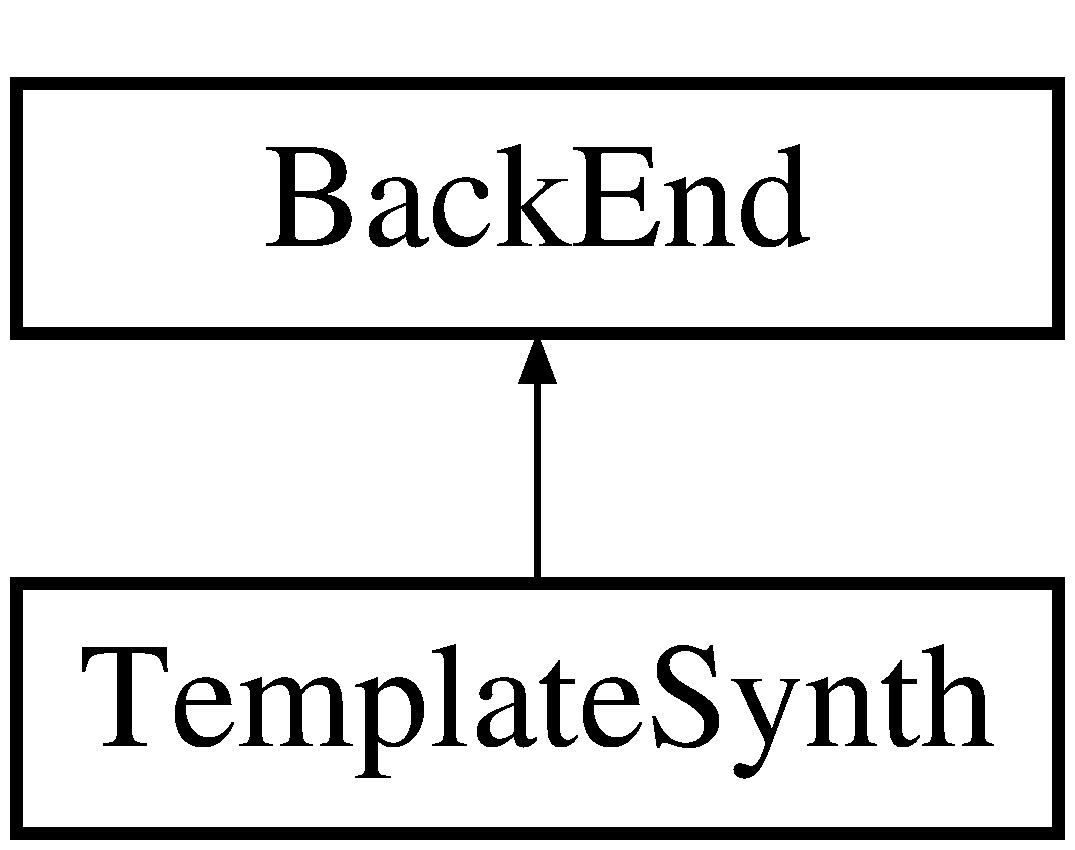
\includegraphics[height=2.000000cm]{classTemplateSynth}
\end{center}
\end{figure}
\subsection*{Public Member Functions}
\begin{DoxyCompactItemize}
\item 
\hyperlink{classTemplateSynth_a56d5f285781e5871bf391acc38acb0aa}{Template\-Synth} (\hyperlink{classCNFImplExtractor}{C\-N\-F\-Impl\-Extractor} $\ast$impl\-\_\-extractor)
\begin{DoxyCompactList}\small\item\em Constructor. \end{DoxyCompactList}\item 
virtual \hyperlink{classTemplateSynth_a5d540c9d4dc6696b53768a27ac74c569}{$\sim$\-Template\-Synth} ()
\begin{DoxyCompactList}\small\item\em Destructor. \end{DoxyCompactList}\item 
virtual bool \hyperlink{classTemplateSynth_a5ad9855736c7d4dfdec08280d2424f80}{run} ()
\begin{DoxyCompactList}\small\item\em Executes this back-\/end. \end{DoxyCompactList}\end{DoxyCompactItemize}
\subsection*{Protected Member Functions}
\begin{DoxyCompactItemize}
\item 
bool \hyperlink{classTemplateSynth_ae334e4a6c30a324cfd4d0c05a32b191c}{compute\-Winning\-Region} ()
\begin{DoxyCompactList}\small\item\em Computes the winning region as instantiation of a generic template. \end{DoxyCompactList}\item 
bool \hyperlink{classTemplateSynth_affe9f11a75e689fd631692feac4031a1}{compute\-Winning\-Region\-C\-N\-F} ()
\begin{DoxyCompactList}\small\item\em Computes the winning region as instantiation of a \hyperlink{classCNF}{C\-N\-F} template. \end{DoxyCompactList}\item 
bool \hyperlink{classTemplateSynth_a9197dff7678cd88a7fea3c6b4358f85d}{compute\-Winning\-Region\-And\-Net} ()
\begin{DoxyCompactList}\small\item\em Computes the winning region as instantiation of a network of A\-N\-D-\/\-Gates. \end{DoxyCompactList}\item 
bool \hyperlink{classTemplateSynth_a499d1c0069b41ce11a6c7e7679fd4ece}{find\-Win\-Reg\-C\-N\-F\-Templ} (size\-\_\-t nr\-\_\-of\-\_\-clauses)
\begin{DoxyCompactList}\small\item\em Computes the winning region as instantiation of a generic \hyperlink{classCNF}{C\-N\-F} template. \end{DoxyCompactList}\item 
bool \hyperlink{classTemplateSynth_a1084d7b10de86dfbbe1368c68d4c0501}{find\-Win\-Reg\-A\-N\-D\-Network} (size\-\_\-t nr\-\_\-of\-\_\-gates)
\begin{DoxyCompactList}\small\item\em Computes the winning region as instantiation of a generic A\-I\-G\-E\-R template. \end{DoxyCompactList}\item 
bool \hyperlink{classTemplateSynth_ae01c9c2463c59f14f109e9379219535b}{synt\-Q\-B\-F} (const \hyperlink{classCNF}{C\-N\-F} \&win\-\_\-constr, int w1, int w2, vector$<$ int $>$ \&solution)
\begin{DoxyCompactList}\small\item\em Resolves the template by calling a Q\-B\-F solver. \end{DoxyCompactList}\item 
bool \hyperlink{classTemplateSynth_aa0f140f63502de21ab260b5cae9335cb}{synt\-S\-A\-T} (const \hyperlink{classCNF}{C\-N\-F} \&win\-\_\-constr, int w1, int w2, vector$<$ int $>$ \&solution)
\begin{DoxyCompactList}\small\item\em Resolves the template by calling a S\-A\-T solver in a C\-E\-G\-I\-S loop. \end{DoxyCompactList}\item 
void \hyperlink{classTemplateSynth_af55609e303daffb4d51b27380d32ddb3}{exclude} (const vector$<$ int $>$ \&ce, const \hyperlink{classCNF}{C\-N\-F} \&gen)
\begin{DoxyCompactList}\small\item\em A helper for the C\-E\-G\-I\-S loop of \hyperlink{classTemplateSynth_aa0f140f63502de21ab260b5cae9335cb}{synt\-S\-A\-T()}, eliminating a counterexample. \end{DoxyCompactList}\item 
bool \hyperlink{classTemplateSynth_a3e841e4eb71a5286057afbeac42c7a47}{check} (const vector$<$ int $>$ \&cand, const \hyperlink{classCNF}{C\-N\-F} \&win\-\_\-constr, int w1, int w2, vector$<$ int $>$ \&ce)
\begin{DoxyCompactList}\small\item\em A helper for the C\-E\-G\-I\-S loop of \hyperlink{classTemplateSynth_aa0f140f63502de21ab260b5cae9335cb}{synt\-S\-A\-T()}, checking if a candidate solution works. \end{DoxyCompactList}\end{DoxyCompactItemize}
\subsection*{Protected Attributes}
\begin{DoxyCompactItemize}
\item 
\hyperlink{classCNF}{C\-N\-F} \hyperlink{classTemplateSynth_a4e147629eae6a542dd87d72902df68c8}{winning\-\_\-region\-\_\-}
\begin{DoxyCompactList}\small\item\em The resulting winning region. \end{DoxyCompactList}\item 
\hyperlink{classCNF}{C\-N\-F} \hyperlink{classTemplateSynth_a49665461c82781b823b3da04057fdab2}{neg\-\_\-winning\-\_\-region\-\_\-}
\begin{DoxyCompactList}\small\item\em The negation of the resulting winning region. \end{DoxyCompactList}\item 
\hyperlink{classQBFSolver}{Q\-B\-F\-Solver} $\ast$ \hyperlink{classTemplateSynth_a08ec20197bf16a10546a7e6cf3719727}{qbf\-\_\-solver\-\_\-}
\begin{DoxyCompactList}\small\item\em The Q\-B\-F-\/solver to use for solving the queries. \end{DoxyCompactList}\item 
\hyperlink{classSatSolver}{Sat\-Solver} $\ast$ \hyperlink{classTemplateSynth_a7844e9296d63b10e3fa96d66b932660f}{sat\-\_\-solver\-\_\-}
\begin{DoxyCompactList}\small\item\em The S\-A\-T-\/solver to use if we resolve the template using the C\-E\-G\-I\-S loop. \end{DoxyCompactList}\item 
\hyperlink{classCNFImplExtractor}{C\-N\-F\-Impl\-Extractor} $\ast$ \hyperlink{classTemplateSynth_acfa25deb001fb3b6d49c0261bba98347}{impl\-\_\-extractor\-\_\-}
\begin{DoxyCompactList}\small\item\em The engine to use for circuit extraction. \end{DoxyCompactList}\end{DoxyCompactItemize}


\subsection{Detailed Description}
Implements a template-\/based synthesis using a Q\-B\-F solver. 

We are searching for a winning region W(x) such that\-: 
\begin{DoxyEnumerate}
\item I(x) =$>$ W(x)\-: every initial state is contained in the winning region 
\item W(x) =$>$ P(x)\-: every state of the winning region is safe 
\item forall x,i\-: exists c,x'\-: W(x) =$>$ (T(x,i,c,x') \& W(x'))\-: from every state in the winning region we can enforce to stay in the winning region by setting the c-\/signals appropriately. 
\end{DoxyEnumerate}In this class, we encode the search for such a winning region symbolically. We define a template W(x,k) for the winning region. The variables k are template parameters. Their values define a concrete function W(x). Then we simply solve the query \par
 ~ exists k\-: forall x,i\-: exists c,x'\-: I(x) =$>$ W(x,k) \& W(x,k) =$>$ P(x) \& W(x,k) =$>$ (T(x,i,c,x') \& W(x',k)) \par
 with a single Q\-B\-F-\/solver call. We ask the solver for a satisfying assignment to the variables k. These values define a concrete function W(x), which is our winning region. The difficult question is how to define a generic template W(x,k) for the winning region. At the moment, only two possibility is implemented\-: 
\begin{DoxyItemize}
\item defining W(x,k) as a parameterized \hyperlink{classCNF}{C\-N\-F} over the state variables x with parameters k. 
\item defining W(x,k) as a parameterized A\-I\-G\-E\-R graph over the state variables x with parameters k 
\end{DoxyItemize}

\begin{DoxyAuthor}{Author}
Robert Koenighofer (\href{mailto:robert.koenighofer@iaik.tugraz.at}{\tt robert.\-koenighofer@iaik.\-tugraz.\-at}) 
\end{DoxyAuthor}
\begin{DoxyVersion}{Version}
1.\-2.\-0 
\end{DoxyVersion}


Definition at line 73 of file Template\-Synth.\-h.



\subsection{Constructor \& Destructor Documentation}
\hypertarget{classTemplateSynth_a56d5f285781e5871bf391acc38acb0aa}{\index{Template\-Synth@{Template\-Synth}!Template\-Synth@{Template\-Synth}}
\index{Template\-Synth@{Template\-Synth}!TemplateSynth@{Template\-Synth}}
\subsubsection[{Template\-Synth}]{\setlength{\rightskip}{0pt plus 5cm}Template\-Synth\-::\-Template\-Synth (
\begin{DoxyParamCaption}
\item[{{\bf C\-N\-F\-Impl\-Extractor} $\ast$}]{impl\-\_\-extractor}
\end{DoxyParamCaption}
)}}\label{classTemplateSynth_a56d5f285781e5871bf391acc38acb0aa}


Constructor. 


\begin{DoxyParams}{Parameters}
{\em impl\-\_\-extractor} & The engine to use for circuit extraction. It will be deleted by this class. \\
\hline
\end{DoxyParams}


Definition at line 44 of file Template\-Synth.\-cpp.

\hypertarget{classTemplateSynth_a5d540c9d4dc6696b53768a27ac74c569}{\index{Template\-Synth@{Template\-Synth}!$\sim$\-Template\-Synth@{$\sim$\-Template\-Synth}}
\index{$\sim$\-Template\-Synth@{$\sim$\-Template\-Synth}!TemplateSynth@{Template\-Synth}}
\subsubsection[{$\sim$\-Template\-Synth}]{\setlength{\rightskip}{0pt plus 5cm}Template\-Synth\-::$\sim$\-Template\-Synth (
\begin{DoxyParamCaption}
{}
\end{DoxyParamCaption}
)\hspace{0.3cm}{\ttfamily [virtual]}}}\label{classTemplateSynth_a5d540c9d4dc6696b53768a27ac74c569}


Destructor. 



Definition at line 54 of file Template\-Synth.\-cpp.



References impl\-\_\-extractor\-\_\-, qbf\-\_\-solver\-\_\-, and sat\-\_\-solver\-\_\-.



\subsection{Member Function Documentation}
\hypertarget{classTemplateSynth_a3e841e4eb71a5286057afbeac42c7a47}{\index{Template\-Synth@{Template\-Synth}!check@{check}}
\index{check@{check}!TemplateSynth@{Template\-Synth}}
\subsubsection[{check}]{\setlength{\rightskip}{0pt plus 5cm}bool Template\-Synth\-::check (
\begin{DoxyParamCaption}
\item[{const vector$<$ int $>$ \&}]{cand, }
\item[{const {\bf C\-N\-F} \&}]{win\-\_\-constr, }
\item[{int}]{w1, }
\item[{int}]{w2, }
\item[{vector$<$ int $>$ \&}]{ce}
\end{DoxyParamCaption}
)\hspace{0.3cm}{\ttfamily [protected]}}}\label{classTemplateSynth_a3e841e4eb71a5286057afbeac42c7a47}


A helper for the C\-E\-G\-I\-S loop of \hyperlink{classTemplateSynth_aa0f140f63502de21ab260b5cae9335cb}{synt\-S\-A\-T()}, checking if a candidate solution works. 


\begin{DoxyParams}{Parameters}
{\em cand} & A canidate solution in the form of concrete values for the template parameters. \\
\hline
{\em win\-\_\-constr} & \hyperlink{classCNF}{C\-N\-F} constraints that constitute a correct solution for the winning region using the generic template. Essentially, three constraints are encoded in this \hyperlink{classCNF}{C\-N\-F}\-: 
\begin{DoxyEnumerate}
\item I(x) =$>$ W(x)\-: every initial state is contained in the winning region 
\item W(x) =$>$ P(x)\-: every state of the winning region is safe 
\item forall x,i\-: exists c,x'\-: W(x) =$>$ (T(x,i,c,x') \& W(x'))\-: from every state in the winning region we can enforce to stay in the winning region by setting the c-\/signals appropriately. 
\end{DoxyEnumerate}\\
\hline
{\em w1} & The literal that represents the present-\/state copy of the winning region in win\-\_\-constr. \\
\hline
{\em w2} & The literal that represents the next-\/state copy of the winning region in win\-\_\-constr. \\
\hline
{\em ce} & An empty vector. If the candidate solution is incorrect, a counterexample in the form of concrete values for state and input variables for which we fall out of the winning region is stored in this vector. \\
\hline
\end{DoxyParams}
\begin{DoxyReturn}{Returns}
True if the candidate solution is correct, False otherwise. 
\end{DoxyReturn}


Definition at line 659 of file Template\-Synth.\-cpp.



References C\-N\-F\-::add1\-Lit\-Clause(), C\-N\-F\-::add\-C\-N\-F(), Var\-Info\-::\-C\-T\-R\-L, Options\-::get\-S\-A\-T\-Solver(), A\-I\-G2\-C\-N\-F\-::get\-Trans(), Var\-Manager\-::get\-Vars\-Of\-Type(), Sat\-Solver\-::inc\-Add\-C\-N\-F(), Sat\-Solver\-::inc\-Add\-Neg\-Cube\-As\-Clause(), Sat\-Solver\-::inc\-Is\-Sat\-Model\-Or\-Core(), Var\-Info\-::\-I\-N\-P\-U\-T, Var\-Manager\-::instance(), Options\-::instance(), A\-I\-G2\-C\-N\-F\-::instance(), M\-A\-S\-S\-E\-R\-T, Var\-Info\-::\-P\-R\-E\-S\-\_\-\-S\-T\-A\-T\-E, C\-N\-F\-::set\-Var\-Value(), and Sat\-Solver\-::start\-Incremental\-Session().



Referenced by synt\-S\-A\-T().

\hypertarget{classTemplateSynth_ae334e4a6c30a324cfd4d0c05a32b191c}{\index{Template\-Synth@{Template\-Synth}!compute\-Winning\-Region@{compute\-Winning\-Region}}
\index{compute\-Winning\-Region@{compute\-Winning\-Region}!TemplateSynth@{Template\-Synth}}
\subsubsection[{compute\-Winning\-Region}]{\setlength{\rightskip}{0pt plus 5cm}bool Template\-Synth\-::compute\-Winning\-Region (
\begin{DoxyParamCaption}
{}
\end{DoxyParamCaption}
)\hspace{0.3cm}{\ttfamily [protected]}}}\label{classTemplateSynth_ae334e4a6c30a324cfd4d0c05a32b191c}


Computes the winning region as instantiation of a generic template. 

This works as explained in the description of the class.

\begin{DoxyReturn}{Returns}
True if the specification was realizable, false otherwise. 
\end{DoxyReturn}


Definition at line 93 of file Template\-Synth.\-cpp.



References compute\-Winning\-Region\-And\-Net(), compute\-Winning\-Region\-C\-N\-F(), and Options\-::instance().



Referenced by run().

\hypertarget{classTemplateSynth_a9197dff7678cd88a7fea3c6b4358f85d}{\index{Template\-Synth@{Template\-Synth}!compute\-Winning\-Region\-And\-Net@{compute\-Winning\-Region\-And\-Net}}
\index{compute\-Winning\-Region\-And\-Net@{compute\-Winning\-Region\-And\-Net}!TemplateSynth@{Template\-Synth}}
\subsubsection[{compute\-Winning\-Region\-And\-Net}]{\setlength{\rightskip}{0pt plus 5cm}bool Template\-Synth\-::compute\-Winning\-Region\-And\-Net (
\begin{DoxyParamCaption}
{}
\end{DoxyParamCaption}
)\hspace{0.3cm}{\ttfamily [protected]}}}\label{classTemplateSynth_a9197dff7678cd88a7fea3c6b4358f85d}


Computes the winning region as instantiation of a network of A\-N\-D-\/\-Gates. 

This works as explained in the description of the class using a A\-I\-G\-E\-R graph template W(x,k) for the winning region W(x), where k are template parameters defining how the winning region really looks like. The A\-I\-G\-E\-R template fixes a maximum number N of A\-N\-D-\/gates. For the first A\-N\-D-\/gate we have template parameters saying (a) which state variables x are an input for the A\-N\-D gate, and (b) which state variables are connected in negated and unnegated form. The second A\-N\-D gate is similar but has the output of the first A\-N\-D gate as additional input. The third A\-N\-D gate has the outputs of the previous two as inputs, and so on. One final template parameter defines whether or not the output of the last A\-N\-D gate forms W(x) or the negation of W(x).

\begin{DoxyReturn}{Returns}
True if the specification was realizable, false otherwise. 
\end{DoxyReturn}


Definition at line 132 of file Template\-Synth.\-cpp.



References find\-Win\-Reg\-A\-N\-D\-Network(), Var\-Manager\-::get\-Vars\-Of\-Type(), Var\-Manager\-::instance(), L\-\_\-\-I\-N\-F, L\-\_\-\-L\-O\-G, Var\-Info\-::\-P\-R\-E\-S\-\_\-\-S\-T\-A\-T\-E, and Var\-Manager\-::reset\-To\-Last\-Push().



Referenced by compute\-Winning\-Region().

\hypertarget{classTemplateSynth_affe9f11a75e689fd631692feac4031a1}{\index{Template\-Synth@{Template\-Synth}!compute\-Winning\-Region\-C\-N\-F@{compute\-Winning\-Region\-C\-N\-F}}
\index{compute\-Winning\-Region\-C\-N\-F@{compute\-Winning\-Region\-C\-N\-F}!TemplateSynth@{Template\-Synth}}
\subsubsection[{compute\-Winning\-Region\-C\-N\-F}]{\setlength{\rightskip}{0pt plus 5cm}bool Template\-Synth\-::compute\-Winning\-Region\-C\-N\-F (
\begin{DoxyParamCaption}
{}
\end{DoxyParamCaption}
)\hspace{0.3cm}{\ttfamily [protected]}}}\label{classTemplateSynth_affe9f11a75e689fd631692feac4031a1}


Computes the winning region as instantiation of a \hyperlink{classCNF}{C\-N\-F} template. 

This works as explained in the description of the class using a \hyperlink{classCNF}{C\-N\-F} template W(x,k) for the winning region W(x), where k are template parameters defining how the winning region really looks like. The \hyperlink{classCNF}{C\-N\-F} template fixes a maximum number N of clauses. It has three groups of parameters. 
\begin{DoxyItemize}
\item The parameters kc\mbox{[}i\mbox{]} (with 1 $<$= i $<$= N) define if clause i occurs in the \hyperlink{classCNF}{C\-N\-F} or not. 
\item The parameters kv\mbox{[}i\mbox{]}\mbox{[}j\mbox{]} (with 1 $<$= i $<$= N, 1 $<$= j $<$= $\vert$x$\vert$) define if state variable xj occurs in clause i or not. 
\item The parameters kn\mbox{[}i\mbox{]}\mbox{[}j\mbox{]} (with 1 $<$= i $<$= N, 1 $<$= j $<$= $\vert$x$\vert$) define if state variable xj occurs in clause i only negated or unnegated. If kv\mbox{[}i\mbox{]}\mbox{[}j\mbox{]}=false, then kn\mbox{[}i\mbox{]}\mbox{[}j\mbox{]} is irrelevant. 
\end{DoxyItemize}The union of all these parameters forms k. Concrete values for all k define a concrete \hyperlink{classCNF}{C\-N\-F} formula over the state variables x (i.\-e., a concrete winning region). We chose N in the following way\-: we start with N=1. On failure, we increase N (multiply by 4).

\begin{DoxyReturn}{Returns}
True if the specification was realizable, false otherwise. 
\end{DoxyReturn}


Definition at line 102 of file Template\-Synth.\-cpp.



References find\-Win\-Reg\-C\-N\-F\-Templ(), Var\-Manager\-::get\-Vars\-Of\-Type(), Var\-Manager\-::instance(), L\-\_\-\-I\-N\-F, L\-\_\-\-L\-O\-G, Var\-Info\-::\-P\-R\-E\-S\-\_\-\-S\-T\-A\-T\-E, and Var\-Manager\-::reset\-To\-Last\-Push().



Referenced by compute\-Winning\-Region().

\hypertarget{classTemplateSynth_af55609e303daffb4d51b27380d32ddb3}{\index{Template\-Synth@{Template\-Synth}!exclude@{exclude}}
\index{exclude@{exclude}!TemplateSynth@{Template\-Synth}}
\subsubsection[{exclude}]{\setlength{\rightskip}{0pt plus 5cm}void Template\-Synth\-::exclude (
\begin{DoxyParamCaption}
\item[{const vector$<$ int $>$ \&}]{ce, }
\item[{const {\bf C\-N\-F} \&}]{gen}
\end{DoxyParamCaption}
)\hspace{0.3cm}{\ttfamily [protected]}}}\label{classTemplateSynth_af55609e303daffb4d51b27380d32ddb3}


A helper for the C\-E\-G\-I\-S loop of \hyperlink{classTemplateSynth_aa0f140f63502de21ab260b5cae9335cb}{synt\-S\-A\-T()}, eliminating a counterexample. 


\begin{DoxyParams}{Parameters}
{\em ce} & A counterexample that has been computed previously by calling \hyperlink{classTemplateSynth_a3e841e4eb71a5286057afbeac42c7a47}{check()}. A counterexample is simply a set of values for state variables and input variables for which we fall out of the winning region. \\
\hline
{\em gen} & The \hyperlink{classCNF}{C\-N\-F} containing the constraints for a correct winning region. We simply add constraints here saying that the winning region must now also work for the counterexample. \\
\hline
\end{DoxyParams}


Definition at line 734 of file Template\-Synth.\-cpp.



References C\-N\-F\-::append\-Vars\-To(), Var\-Manager\-::create\-Fresh\-Tmp\-Var(), Var\-Manager\-::get\-Info(), Var\-Info\-::get\-Kind(), Sat\-Solver\-::inc\-Add\-C\-N\-F(), Var\-Manager\-::instance(), C\-N\-F\-::rename\-Vars(), sat\-\_\-solver\-\_\-, C\-N\-F\-::set\-Var\-Value(), and Var\-Info\-::\-T\-E\-M\-P\-L\-\_\-\-P\-A\-R\-A\-M\-S.



Referenced by synt\-S\-A\-T().

\hypertarget{classTemplateSynth_a1084d7b10de86dfbbe1368c68d4c0501}{\index{Template\-Synth@{Template\-Synth}!find\-Win\-Reg\-A\-N\-D\-Network@{find\-Win\-Reg\-A\-N\-D\-Network}}
\index{find\-Win\-Reg\-A\-N\-D\-Network@{find\-Win\-Reg\-A\-N\-D\-Network}!TemplateSynth@{Template\-Synth}}
\subsubsection[{find\-Win\-Reg\-A\-N\-D\-Network}]{\setlength{\rightskip}{0pt plus 5cm}bool Template\-Synth\-::find\-Win\-Reg\-A\-N\-D\-Network (
\begin{DoxyParamCaption}
\item[{size\-\_\-t}]{nr\-\_\-of\-\_\-gates}
\end{DoxyParamCaption}
)\hspace{0.3cm}{\ttfamily [protected]}}}\label{classTemplateSynth_a1084d7b10de86dfbbe1368c68d4c0501}


Computes the winning region as instantiation of a generic A\-I\-G\-E\-R template. 

This works as explained in the description of \hyperlink{classTemplateSynth_a9197dff7678cd88a7fea3c6b4358f85d}{compute\-Winning\-Region\-And\-Net()}.


\begin{DoxyParams}{Parameters}
{\em nr\-\_\-of\-\_\-gates} & The number N of gates to use in the template. Choosing a good value for this parameter is difficult. If it is chosen to low, then we may not find a solution even if one exists. If it is chosen to high, then we waste computational resources. \\
\hline
\end{DoxyParams}
\begin{DoxyReturn}{Returns}
True if a solution is found with the given number of clauses, false otherwise. If this method returns false, then this does not mean that the specification is unrealizable. It may be that nr\-\_\-of\-\_\-gates has been chosen too low. 
\end{DoxyReturn}


Definition at line 335 of file Template\-Synth.\-cpp.



References C\-N\-F\-::add1\-Lit\-Clause(), C\-N\-F\-::add2\-Lit\-Clause(), C\-N\-F\-::add4\-Lit\-Clause(), C\-N\-F\-::add\-Clause(), Var\-Manager\-::create\-Fresh\-Templ\-Param(), Var\-Manager\-::create\-Fresh\-Tmp\-Var(), Var\-Manager\-::get\-Next\-Error\-State\-Var(), Var\-Manager\-::get\-Pres\-Error\-State\-Var(), Var\-Manager\-::get\-Vars\-Of\-Type(), Var\-Manager\-::instance(), Options\-::instance(), neg\-\_\-winning\-\_\-region\-\_\-, Utils\-::negate\-Literals(), Var\-Info\-::\-N\-E\-X\-T\-\_\-\-S\-T\-A\-T\-E, Var\-Info\-::\-P\-R\-E\-S\-\_\-\-S\-T\-A\-T\-E, Var\-Manager\-::reset\-To\-Last\-Push(), synt\-Q\-B\-F(), synt\-S\-A\-T(), Var\-Info\-::\-T\-E\-M\-P\-L\-\_\-\-P\-A\-R\-A\-M\-S, and winning\-\_\-region\-\_\-.



Referenced by compute\-Winning\-Region\-And\-Net().

\hypertarget{classTemplateSynth_a499d1c0069b41ce11a6c7e7679fd4ece}{\index{Template\-Synth@{Template\-Synth}!find\-Win\-Reg\-C\-N\-F\-Templ@{find\-Win\-Reg\-C\-N\-F\-Templ}}
\index{find\-Win\-Reg\-C\-N\-F\-Templ@{find\-Win\-Reg\-C\-N\-F\-Templ}!TemplateSynth@{Template\-Synth}}
\subsubsection[{find\-Win\-Reg\-C\-N\-F\-Templ}]{\setlength{\rightskip}{0pt plus 5cm}bool Template\-Synth\-::find\-Win\-Reg\-C\-N\-F\-Templ (
\begin{DoxyParamCaption}
\item[{size\-\_\-t}]{nr\-\_\-of\-\_\-clauses}
\end{DoxyParamCaption}
)\hspace{0.3cm}{\ttfamily [protected]}}}\label{classTemplateSynth_a499d1c0069b41ce11a6c7e7679fd4ece}


Computes the winning region as instantiation of a generic \hyperlink{classCNF}{C\-N\-F} template. 

This works as explained in the description of \hyperlink{classTemplateSynth_affe9f11a75e689fd631692feac4031a1}{compute\-Winning\-Region\-C\-N\-F()}.


\begin{DoxyParams}{Parameters}
{\em nr\-\_\-of\-\_\-clauses} & The number N of clauses to use in the template. Choosing a good value for this parameter is difficult. If it is chosen to low, then we may not find a solution even if one exists. If it is chosen to high, then we waste computational resources. \\
\hline
\end{DoxyParams}
\begin{DoxyReturn}{Returns}
True if a solution is found with the given number of clauses, false otherwise. If this method returns false, then this does not mean that the specification is unrealizable. It may be that nr\-\_\-of\-\_\-clauses has been chosen too low. 
\end{DoxyReturn}


Definition at line 162 of file Template\-Synth.\-cpp.



References C\-N\-F\-::add1\-Lit\-Clause(), C\-N\-F\-::add2\-Lit\-Clause(), C\-N\-F\-::add4\-Lit\-Clause(), C\-N\-F\-::add\-Clause(), Var\-Manager\-::create\-Fresh\-Templ\-Param(), Var\-Manager\-::create\-Fresh\-Tmp\-Var(), Var\-Manager\-::get\-Max\-C\-N\-F\-Var(), Var\-Manager\-::get\-Next\-Error\-State\-Var(), Var\-Manager\-::get\-Pres\-Error\-State\-Var(), Var\-Manager\-::get\-Vars\-Of\-Type(), Var\-Manager\-::instance(), Options\-::instance(), neg\-\_\-winning\-\_\-region\-\_\-, C\-N\-F\-::negate(), Var\-Info\-::\-N\-E\-X\-T\-\_\-\-S\-T\-A\-T\-E, Var\-Info\-::\-P\-R\-E\-S\-\_\-\-S\-T\-A\-T\-E, Var\-Manager\-::reset\-To\-Last\-Push(), synt\-Q\-B\-F(), synt\-S\-A\-T(), and winning\-\_\-region\-\_\-.



Referenced by compute\-Winning\-Region\-C\-N\-F().

\hypertarget{classTemplateSynth_a5ad9855736c7d4dfdec08280d2424f80}{\index{Template\-Synth@{Template\-Synth}!run@{run}}
\index{run@{run}!TemplateSynth@{Template\-Synth}}
\subsubsection[{run}]{\setlength{\rightskip}{0pt plus 5cm}bool Template\-Synth\-::run (
\begin{DoxyParamCaption}
{}
\end{DoxyParamCaption}
)\hspace{0.3cm}{\ttfamily [virtual]}}}\label{classTemplateSynth_a5ad9855736c7d4dfdec08280d2424f80}


Executes this back-\/end. 

The back-\/end works as explained in the description of the class.

\begin{DoxyReturn}{Returns}
True if the specification was realizable, false otherwise. 
\end{DoxyReturn}


Implements \hyperlink{classBackEnd_a099e717dc71e9cc2d838b1ca86340590}{Back\-End}.



Definition at line 67 of file Template\-Synth.\-cpp.



References compute\-Winning\-Region(), Utils\-::debug\-Check\-Win\-Reg(), C\-N\-F\-Impl\-Extractor\-::extract\-Circuit(), impl\-\_\-extractor\-\_\-, Var\-Manager\-::instance(), Options\-::instance(), L\-\_\-\-I\-N\-F, L\-\_\-\-R\-E\-S, C\-N\-F\-Impl\-Extractor\-::log\-Statistics(), neg\-\_\-winning\-\_\-region\-\_\-, Var\-Manager\-::push(), and winning\-\_\-region\-\_\-.

\hypertarget{classTemplateSynth_ae01c9c2463c59f14f109e9379219535b}{\index{Template\-Synth@{Template\-Synth}!synt\-Q\-B\-F@{synt\-Q\-B\-F}}
\index{synt\-Q\-B\-F@{synt\-Q\-B\-F}!TemplateSynth@{Template\-Synth}}
\subsubsection[{synt\-Q\-B\-F}]{\setlength{\rightskip}{0pt plus 5cm}bool Template\-Synth\-::synt\-Q\-B\-F (
\begin{DoxyParamCaption}
\item[{const {\bf C\-N\-F} \&}]{win\-\_\-constr, }
\item[{int}]{w1, }
\item[{int}]{w2, }
\item[{vector$<$ int $>$ \&}]{solution}
\end{DoxyParamCaption}
)\hspace{0.3cm}{\ttfamily [protected]}}}\label{classTemplateSynth_ae01c9c2463c59f14f109e9379219535b}


Resolves the template by calling a Q\-B\-F solver. 


\begin{DoxyParams}{Parameters}
{\em win\-\_\-constr} & \hyperlink{classCNF}{C\-N\-F} constraints that constitute a correct solution for the winning region using the generic template. Essentially, three constraints are encoded in this \hyperlink{classCNF}{C\-N\-F}\-: 
\begin{DoxyEnumerate}
\item I(x) =$>$ W(x)\-: every initial state is contained in the winning region 
\item W(x) =$>$ P(x)\-: every state of the winning region is safe 
\item forall x,i\-: exists c,x'\-: W(x) =$>$ (T(x,i,c,x') \& W(x'))\-: from every state in the winning region we can enforce to stay in the winning region by setting the c-\/signals appropriately. 
\end{DoxyEnumerate}\\
\hline
{\em w1} & The literal that represents the present-\/state copy of the winning region in win\-\_\-constr. \\
\hline
{\em w2} & The literal that represents the next-\/state copy of the winning region in win\-\_\-constr. \\
\hline
{\em solution} & An empty vector. If a solution exists, then the corresponding template parameter values are written into this vector. \\
\hline
\end{DoxyParams}
\begin{DoxyReturn}{Returns}
True if a solution exists, false otherwise. 
\end{DoxyReturn}


Definition at line 575 of file Template\-Synth.\-cpp.



References Q\-B\-F\-Solver\-::\-A, C\-N\-F\-::add\-C\-N\-F(), Var\-Info\-::\-C\-T\-R\-L, Q\-B\-F\-Solver\-::\-E, A\-I\-G2\-C\-N\-F\-::get\-T(), A\-I\-G2\-C\-N\-F\-::get\-Trans\-Eq\-T(), Var\-Manager\-::get\-Vars\-Of\-Type(), Var\-Info\-::\-I\-N\-P\-U\-T, Var\-Manager\-::instance(), A\-I\-G2\-C\-N\-F\-::instance(), Q\-B\-F\-Solver\-::is\-Sat\-Model(), Var\-Info\-::\-N\-E\-X\-T\-\_\-\-S\-T\-A\-T\-E, Var\-Info\-::\-P\-R\-E\-S\-\_\-\-S\-T\-A\-T\-E, qbf\-\_\-solver\-\_\-, Var\-Info\-::\-T\-E\-M\-P\-L\-\_\-\-P\-A\-R\-A\-M\-S, and Var\-Info\-::\-T\-M\-P.



Referenced by find\-Win\-Reg\-A\-N\-D\-Network(), and find\-Win\-Reg\-C\-N\-F\-Templ().

\hypertarget{classTemplateSynth_aa0f140f63502de21ab260b5cae9335cb}{\index{Template\-Synth@{Template\-Synth}!synt\-S\-A\-T@{synt\-S\-A\-T}}
\index{synt\-S\-A\-T@{synt\-S\-A\-T}!TemplateSynth@{Template\-Synth}}
\subsubsection[{synt\-S\-A\-T}]{\setlength{\rightskip}{0pt plus 5cm}bool Template\-Synth\-::synt\-S\-A\-T (
\begin{DoxyParamCaption}
\item[{const {\bf C\-N\-F} \&}]{win\-\_\-constr, }
\item[{int}]{w1, }
\item[{int}]{w2, }
\item[{vector$<$ int $>$ \&}]{solution}
\end{DoxyParamCaption}
)\hspace{0.3cm}{\ttfamily [protected]}}}\label{classTemplateSynth_aa0f140f63502de21ab260b5cae9335cb}


Resolves the template by calling a S\-A\-T solver in a C\-E\-G\-I\-S loop. 


\begin{DoxyParams}{Parameters}
{\em win\-\_\-constr} & \hyperlink{classCNF}{C\-N\-F} constraints that constitute a correct solution for the winning region using the generic template. Essentially, three constraints are encoded in this \hyperlink{classCNF}{C\-N\-F}\-: 
\begin{DoxyEnumerate}
\item I(x) =$>$ W(x)\-: every initial state is contained in the winning region 
\item W(x) =$>$ P(x)\-: every state of the winning region is safe 
\item forall x,i\-: exists c,x'\-: W(x) =$>$ (T(x,i,c,x') \& W(x'))\-: from every state in the winning region we can enforce to stay in the winning region by setting the c-\/signals appropriately. 
\end{DoxyEnumerate}\\
\hline
{\em w1} & The literal that represents the present-\/state copy of the winning region in win\-\_\-constr. \\
\hline
{\em w2} & The literal that represents the next-\/state copy of the winning region in win\-\_\-constr. \\
\hline
{\em solution} & An empty vector. If a solution exists, then the corresponding template parameter values are written into this vector. \\
\hline
\end{DoxyParams}
\begin{DoxyReturn}{Returns}
True if a solution exists, false otherwise. 
\end{DoxyReturn}


Definition at line 607 of file Template\-Synth.\-cpp.



References C\-N\-F\-::add\-C\-N\-F(), check(), exclude(), A\-I\-G2\-C\-N\-F\-::get\-Trans(), Var\-Manager\-::get\-Vars\-Of\-Type(), Sat\-Solver\-::inc\-Is\-Sat\-Model\-Or\-Core(), Var\-Info\-::\-I\-N\-P\-U\-T, Var\-Manager\-::instance(), A\-I\-G2\-C\-N\-F\-::instance(), Utils\-::negate\-Literals(), Var\-Info\-::\-P\-R\-E\-S\-\_\-\-S\-T\-A\-T\-E, sat\-\_\-solver\-\_\-, Sat\-Solver\-::start\-Incremental\-Session(), and Var\-Info\-::\-T\-E\-M\-P\-L\-\_\-\-P\-A\-R\-A\-M\-S.



Referenced by find\-Win\-Reg\-A\-N\-D\-Network(), and find\-Win\-Reg\-C\-N\-F\-Templ().



\subsection{Member Data Documentation}
\hypertarget{classTemplateSynth_acfa25deb001fb3b6d49c0261bba98347}{\index{Template\-Synth@{Template\-Synth}!impl\-\_\-extractor\-\_\-@{impl\-\_\-extractor\-\_\-}}
\index{impl\-\_\-extractor\-\_\-@{impl\-\_\-extractor\-\_\-}!TemplateSynth@{Template\-Synth}}
\subsubsection[{impl\-\_\-extractor\-\_\-}]{\setlength{\rightskip}{0pt plus 5cm}{\bf C\-N\-F\-Impl\-Extractor}$\ast$ Template\-Synth\-::impl\-\_\-extractor\-\_\-\hspace{0.3cm}{\ttfamily [protected]}}}\label{classTemplateSynth_acfa25deb001fb3b6d49c0261bba98347}


The engine to use for circuit extraction. 

It will be deleted by this class (in the destructor). 

Definition at line 290 of file Template\-Synth.\-h.



Referenced by run(), and $\sim$\-Template\-Synth().

\hypertarget{classTemplateSynth_a49665461c82781b823b3da04057fdab2}{\index{Template\-Synth@{Template\-Synth}!neg\-\_\-winning\-\_\-region\-\_\-@{neg\-\_\-winning\-\_\-region\-\_\-}}
\index{neg\-\_\-winning\-\_\-region\-\_\-@{neg\-\_\-winning\-\_\-region\-\_\-}!TemplateSynth@{Template\-Synth}}
\subsubsection[{neg\-\_\-winning\-\_\-region\-\_\-}]{\setlength{\rightskip}{0pt plus 5cm}{\bf C\-N\-F} Template\-Synth\-::neg\-\_\-winning\-\_\-region\-\_\-\hspace{0.3cm}{\ttfamily [protected]}}}\label{classTemplateSynth_a49665461c82781b823b3da04057fdab2}


The negation of the resulting winning region. 



Definition at line 273 of file Template\-Synth.\-h.



Referenced by find\-Win\-Reg\-A\-N\-D\-Network(), find\-Win\-Reg\-C\-N\-F\-Templ(), and run().

\hypertarget{classTemplateSynth_a08ec20197bf16a10546a7e6cf3719727}{\index{Template\-Synth@{Template\-Synth}!qbf\-\_\-solver\-\_\-@{qbf\-\_\-solver\-\_\-}}
\index{qbf\-\_\-solver\-\_\-@{qbf\-\_\-solver\-\_\-}!TemplateSynth@{Template\-Synth}}
\subsubsection[{qbf\-\_\-solver\-\_\-}]{\setlength{\rightskip}{0pt plus 5cm}{\bf Q\-B\-F\-Solver}$\ast$ Template\-Synth\-::qbf\-\_\-solver\-\_\-\hspace{0.3cm}{\ttfamily [protected]}}}\label{classTemplateSynth_a08ec20197bf16a10546a7e6cf3719727}


The Q\-B\-F-\/solver to use for solving the queries. 



Definition at line 278 of file Template\-Synth.\-h.



Referenced by synt\-Q\-B\-F(), and $\sim$\-Template\-Synth().

\hypertarget{classTemplateSynth_a7844e9296d63b10e3fa96d66b932660f}{\index{Template\-Synth@{Template\-Synth}!sat\-\_\-solver\-\_\-@{sat\-\_\-solver\-\_\-}}
\index{sat\-\_\-solver\-\_\-@{sat\-\_\-solver\-\_\-}!TemplateSynth@{Template\-Synth}}
\subsubsection[{sat\-\_\-solver\-\_\-}]{\setlength{\rightskip}{0pt plus 5cm}{\bf Sat\-Solver}$\ast$ Template\-Synth\-::sat\-\_\-solver\-\_\-\hspace{0.3cm}{\ttfamily [protected]}}}\label{classTemplateSynth_a7844e9296d63b10e3fa96d66b932660f}


The S\-A\-T-\/solver to use if we resolve the template using the C\-E\-G\-I\-S loop. 



Definition at line 283 of file Template\-Synth.\-h.



Referenced by exclude(), synt\-S\-A\-T(), and $\sim$\-Template\-Synth().

\hypertarget{classTemplateSynth_a4e147629eae6a542dd87d72902df68c8}{\index{Template\-Synth@{Template\-Synth}!winning\-\_\-region\-\_\-@{winning\-\_\-region\-\_\-}}
\index{winning\-\_\-region\-\_\-@{winning\-\_\-region\-\_\-}!TemplateSynth@{Template\-Synth}}
\subsubsection[{winning\-\_\-region\-\_\-}]{\setlength{\rightskip}{0pt plus 5cm}{\bf C\-N\-F} Template\-Synth\-::winning\-\_\-region\-\_\-\hspace{0.3cm}{\ttfamily [protected]}}}\label{classTemplateSynth_a4e147629eae6a542dd87d72902df68c8}


The resulting winning region. 



Definition at line 268 of file Template\-Synth.\-h.



Referenced by find\-Win\-Reg\-A\-N\-D\-Network(), find\-Win\-Reg\-C\-N\-F\-Templ(), and run().



The documentation for this class was generated from the following files\-:\begin{DoxyCompactItemize}
\item 
src/\hyperlink{TemplateSynth_8h}{Template\-Synth.\-h}\item 
src/\hyperlink{TemplateSynth_8cpp}{Template\-Synth.\-cpp}\end{DoxyCompactItemize}

\hypertarget{classUtils}{\section{Utils Class Reference}
\label{classUtils}\index{Utils@{Utils}}
}


Contains utility functions that can be usful in various back-\/ends.  




{\ttfamily \#include $<$Utils.\-h$>$}

\subsection*{Static Public Member Functions}
\begin{DoxyCompactItemize}
\item 
static bool \hyperlink{classUtils_adef5db58221c7a04397de10ec0b13fb6}{contains\-Init} (const vector$<$ int $>$ \&cube)
\begin{DoxyCompactList}\small\item\em Checks if a cube (in form of a vector of literals) contains the initial state. \end{DoxyCompactList}\item 
static bool \hyperlink{classUtils_a02ae74e9866b8ca0863c9507e46df007}{contains\-Init} (const set$<$ int $>$ \&cube)
\begin{DoxyCompactList}\small\item\em Checks if a cube (in form of a set of literals) contains the initial state. \end{DoxyCompactList}\item 
static vector$<$ int $>$ \hyperlink{classUtils_a9eb9e182ca1da6a1050338928083f632}{extract} (const vector$<$ int $>$ \&cube\-\_\-or\-\_\-clause, \hyperlink{classVarInfo_a64d1da76cf84fe674e5fef9764ef11cf}{Var\-Info\-::\-Var\-Kind} kind)
\begin{DoxyCompactList}\small\item\em Extracts literals that are of a given type from a cube or clause. \end{DoxyCompactList}\item 
static vector$<$ int $>$ \hyperlink{classUtils_a9c060a97bf0e9e5e08bf33b512633ac3}{extract\-Pres\-In} (const vector$<$ int $>$ \&cube\-\_\-or\-\_\-clause)
\begin{DoxyCompactList}\small\item\em Extracts present-\/state literals and input literals from a cube or clause. \end{DoxyCompactList}\item 
static vector$<$ int $>$ \hyperlink{classUtils_a9251f04947864aaaac7e459987913429}{extract\-Next\-As\-Present} (const vector$<$ int $>$ \&cube\-\_\-or\-\_\-clause)
\begin{DoxyCompactList}\small\item\em Extracts next-\/state literals and returns the present-\/state copy. \end{DoxyCompactList}\item 
static vector$<$ int $>$ \hyperlink{classUtils_a21f2b014ac53ca027864c57e24a60195}{extract} (const vector$<$ int $>$ \&cube\-\_\-or\-\_\-clause, const vector$<$ int $>$ \&vars)
\begin{DoxyCompactList}\small\item\em Extracts certain literals from a cube or clause. \end{DoxyCompactList}\item 
static void \hyperlink{classUtils_a71efa1aa570b356a328e95008fb65ad8}{randomize} (vector$<$ int $>$ \&vec)
\begin{DoxyCompactList}\small\item\em Randomizes the order (not the value) of a given vector of integers. \end{DoxyCompactList}\item 
static void \hyperlink{classUtils_a2843ae3d849c66ebd72baea26fbd7580}{sort} (vector$<$ int $>$ \&vec)
\begin{DoxyCompactList}\small\item\em Sorts a vector of integers in ascending order. \end{DoxyCompactList}\item 
static bool \hyperlink{classUtils_a15b142132eb40445f51b1f1bb89b85f3}{remove} (vector$<$ int $>$ \&vec, int elem)
\begin{DoxyCompactList}\small\item\em Removes a certain element from a vector. \end{DoxyCompactList}\item 
static bool \hyperlink{classUtils_a84611c8a027ac12426219cb4d59765aa}{contains} (const vector$<$ int $>$ \&vec, int elem)
\begin{DoxyCompactList}\small\item\em Checks if a vector contains a certain element. \end{DoxyCompactList}\item 
static bool \hyperlink{classUtils_a5dc062d4cf872c0d69924116879715ab}{eq} (const vector$<$ int $>$ \&v1, const vector$<$ int $>$ \&v2, int start\-\_\-idx=0)
\begin{DoxyCompactList}\small\item\em Checks if two vectors contain the same set of elements. \end{DoxyCompactList}\item 
static void \hyperlink{classUtils_ae7584589e0d06005fe893fdb9244483a}{negate\-Literals} (vector$<$ int $>$ \&cube\-\_\-or\-\_\-clause)
\begin{DoxyCompactList}\small\item\em Negates all literals in a cube or clause. \end{DoxyCompactList}\item 
static void \hyperlink{classUtils_a8e0d236cf00a61a34ef5c48bcb08a1ec}{swap\-Present\-To\-Next} (vector$<$ int $>$ \&vec)
\begin{DoxyCompactList}\small\item\em Replaces all current-\/state literals by their next-\/state copy. \end{DoxyCompactList}\item 
static bool \hyperlink{classUtils_aa6a513b0ad3b22b3b857060219c222d6}{intersection\-Empty} (const vector$<$ int $>$ \&x, const set$<$ int $>$ \&y)
\begin{DoxyCompactList}\small\item\em Checks if a vector and a set have an empty intersection. \end{DoxyCompactList}\item 
static bool \hyperlink{classUtils_ae957d76f82e729f9d127cf05cb61320d}{intersection\-Empty} (const set$<$ int $>$ \&x, const set$<$ int $>$ \&y)
\begin{DoxyCompactList}\small\item\em Checks if the intersection of two sets is empty. \end{DoxyCompactList}\item 
static bool \hyperlink{classUtils_ab5dca8125b6addaa1f0331664ab6142e}{is\-Subset} (const vector$<$ int $>$ \&subset, const vector$<$ int $>$ \&superset)
\begin{DoxyCompactList}\small\item\em Checks if one vector forms a subset of another one. \end{DoxyCompactList}\item 
static bool \hyperlink{classUtils_ac4e713aa386834b587e2695855fbc27a}{compress\-State\-C\-N\-F} (\hyperlink{classCNF}{C\-N\-F} \&cnf, bool hardcore=false)
\begin{DoxyCompactList}\small\item\em Compresses a state-\/\-C\-N\-F by removing clauses that are implied by others. \end{DoxyCompactList}\item 
static void \hyperlink{classUtils_ad6bc8cf6342b8f182597aa53cf72d9d3}{negate\-State\-C\-N\-F} (\hyperlink{classCNF}{C\-N\-F} \&cnf)
\begin{DoxyCompactList}\small\item\em Negates a \hyperlink{classCNF}{C\-N\-F} over the state-\/variables without introducing temporary variables. \end{DoxyCompactList}\item 
static void \hyperlink{classUtils_acd64e5ea20bd4579427734a9ede171d8}{negate\-Via\-Aig} (\hyperlink{classCNF}{C\-N\-F} \&cnf)
\begin{DoxyCompactList}\small\item\em Negates a \hyperlink{classCNF}{C\-N\-F} by transforming into A\-I\-G\-E\-R and back. \end{DoxyCompactList}\item 
static void \hyperlink{classUtils_a5ddf6a703833a37aae073e12d114a6c8}{compress\-Next\-State\-C\-N\-F} (\hyperlink{classCNF}{C\-N\-F} \&ps\-\_\-cnf, \hyperlink{classCNF}{C\-N\-F} \&ns\-\_\-cnf, bool hardcore=false)
\begin{DoxyCompactList}\small\item\em Compresses a state-\/\-C\-N\-F by removing implied clauses and computes the next-\/state \hyperlink{classCNF}{C\-N\-F}. \end{DoxyCompactList}\item 
static size\-\_\-t \hyperlink{classUtils_ae48658c2b3c7f71261146210c7861b60}{get\-Current\-Mem\-Usage} ()
\begin{DoxyCompactList}\small\item\em Returns the current memory usage as debug message in k\-B. \end{DoxyCompactList}\item 
static void \hyperlink{classUtils_adeaccd2a53073b17e3409eab8e98db0c}{debug\-Print} (const vector$<$ int $>$ \&vec, string prefix=\char`\"{}\char`\"{})
\begin{DoxyCompactList}\small\item\em Prints a vector of literals (mainly for debugging purposes). \end{DoxyCompactList}\item 
static void \hyperlink{classUtils_acc29602987b73022546a6d752a7e093f}{debug\-Check\-Win\-Reg} (const \hyperlink{classCNF}{C\-N\-F} \&winning\-\_\-region)
\begin{DoxyCompactList}\small\item\em Checks a winning region for correctness. \end{DoxyCompactList}\item 
static void \hyperlink{classUtils_a448f5356530d2e88fa9928f4ed857238}{debug\-Check\-Win\-Reg} (const \hyperlink{classCNF}{C\-N\-F} \&winning\-\_\-region, const \hyperlink{classCNF}{C\-N\-F} \&neg\-\_\-winning\-\_\-region)
\begin{DoxyCompactList}\small\item\em Checks a winning region and its negation for correctness. \end{DoxyCompactList}\item 
static void \hyperlink{classUtils_af69b7f70358d1c1616aab1560c7363cd}{debug\-Print\-Current\-Mem\-Usage} ()
\begin{DoxyCompactList}\small\item\em Prints the current memory usage as debug message. \end{DoxyCompactList}\end{DoxyCompactItemize}
\subsection*{Private Member Functions}
\begin{DoxyCompactItemize}
\item 
\hyperlink{classUtils_a452e78692c87ed5c7c993b6c6ac4981a}{Utils} ()
\begin{DoxyCompactList}\small\item\em Constructor. \end{DoxyCompactList}\item 
virtual \hyperlink{classUtils_a0d842a927296003dd7088fc1e4e2a367}{$\sim$\-Utils} ()
\begin{DoxyCompactList}\small\item\em Constructor. \end{DoxyCompactList}\item 
\hyperlink{classUtils_a80726f8ec2ed2707a8bfd4fd355ef27a}{Utils} (const \hyperlink{classUtils}{Utils} \&other)
\begin{DoxyCompactList}\small\item\em Copy constructor. \end{DoxyCompactList}\item 
\hyperlink{classUtils}{Utils} \& \hyperlink{classUtils_a0ed61b802f94ec15000c458e9aae4f19}{operator=} (const \hyperlink{classUtils}{Utils} \&other)
\begin{DoxyCompactList}\small\item\em Assignment operator. \end{DoxyCompactList}\end{DoxyCompactItemize}


\subsection{Detailed Description}
Contains utility functions that can be usful in various back-\/ends. 

\begin{DoxyAuthor}{Author}
Robert Koenighofer (\href{mailto:robert.koenighofer@iaik.tugraz.at}{\tt robert.\-koenighofer@iaik.\-tugraz.\-at}) 
\end{DoxyAuthor}
\begin{DoxyVersion}{Version}
1.\-2.\-0 
\end{DoxyVersion}


Definition at line 45 of file Utils.\-h.



\subsection{Constructor \& Destructor Documentation}
\hypertarget{classUtils_a452e78692c87ed5c7c993b6c6ac4981a}{\index{Utils@{Utils}!Utils@{Utils}}
\index{Utils@{Utils}!Utils@{Utils}}
\subsubsection[{Utils}]{\setlength{\rightskip}{0pt plus 5cm}Utils\-::\-Utils (
\begin{DoxyParamCaption}
{}
\end{DoxyParamCaption}
)\hspace{0.3cm}{\ttfamily [private]}}}\label{classUtils_a452e78692c87ed5c7c993b6c6ac4981a}


Constructor. 

The constructor is private and not implemented. Use the static methods. \hypertarget{classUtils_a0d842a927296003dd7088fc1e4e2a367}{\index{Utils@{Utils}!$\sim$\-Utils@{$\sim$\-Utils}}
\index{$\sim$\-Utils@{$\sim$\-Utils}!Utils@{Utils}}
\subsubsection[{$\sim$\-Utils}]{\setlength{\rightskip}{0pt plus 5cm}virtual Utils\-::$\sim$\-Utils (
\begin{DoxyParamCaption}
{}
\end{DoxyParamCaption}
)\hspace{0.3cm}{\ttfamily [private]}, {\ttfamily [virtual]}}}\label{classUtils_a0d842a927296003dd7088fc1e4e2a367}


Constructor. 

The constructor is private and not implemented. Use the static methods. \hypertarget{classUtils_a80726f8ec2ed2707a8bfd4fd355ef27a}{\index{Utils@{Utils}!Utils@{Utils}}
\index{Utils@{Utils}!Utils@{Utils}}
\subsubsection[{Utils}]{\setlength{\rightskip}{0pt plus 5cm}Utils\-::\-Utils (
\begin{DoxyParamCaption}
\item[{const {\bf Utils} \&}]{other}
\end{DoxyParamCaption}
)\hspace{0.3cm}{\ttfamily [private]}}}\label{classUtils_a80726f8ec2ed2707a8bfd4fd355ef27a}


Copy constructor. 

The copy constructor is disabled (set private) and not implemented.


\begin{DoxyParams}{Parameters}
{\em other} & The source for creating the copy. \\
\hline
\end{DoxyParams}


\subsection{Member Function Documentation}
\hypertarget{classUtils_a5ddf6a703833a37aae073e12d114a6c8}{\index{Utils@{Utils}!compress\-Next\-State\-C\-N\-F@{compress\-Next\-State\-C\-N\-F}}
\index{compress\-Next\-State\-C\-N\-F@{compress\-Next\-State\-C\-N\-F}!Utils@{Utils}}
\subsubsection[{compress\-Next\-State\-C\-N\-F}]{\setlength{\rightskip}{0pt plus 5cm}void Utils\-::compress\-Next\-State\-C\-N\-F (
\begin{DoxyParamCaption}
\item[{{\bf C\-N\-F} \&}]{ps\-\_\-cnf, }
\item[{{\bf C\-N\-F} \&}]{ns\-\_\-cnf, }
\item[{bool}]{hardcore = {\ttfamily false}}
\end{DoxyParamCaption}
)\hspace{0.3cm}{\ttfamily [static]}}}\label{classUtils_a5ddf6a703833a37aae073e12d114a6c8}


Compresses a state-\/\-C\-N\-F by removing implied clauses and computes the next-\/state \hyperlink{classCNF}{C\-N\-F}. 

This method is similar to \hyperlink{classUtils_ac4e713aa386834b587e2695855fbc27a}{compress\-State\-C\-N\-F()}. The difference is that this method also computes a compact representation of the next-\/state copy of passed state-\/\-C\-N\-F. When compressing the next-\/state copy, clauses are removed if they are already implied by existing clauses or the present-\/state copy of the \hyperlink{classCNF}{C\-N\-F}. That is, the compression of the next-\/state copy is only valid if the current-\/state copy is going to be asserted in the solver. 
\begin{DoxyParams}{Parameters}
{\em ps\-\_\-cnf} & The \hyperlink{classCNF}{C\-N\-F} formula to compress. We assume that this \hyperlink{classCNF}{C\-N\-F} only talks about the present-\/state variables. This \hyperlink{classCNF}{C\-N\-F} is compressed, similar as done by \hyperlink{classUtils_ac4e713aa386834b587e2695855fbc27a}{compress\-State\-C\-N\-F()}. \\
\hline
{\em ns\-\_\-cnf} & An empty \hyperlink{classCNF}{C\-N\-F}. This \hyperlink{classCNF}{C\-N\-F} is filled with the compression of the next-\/state copy of ps\-\_\-cnf. The resulting ns\-\_\-cnf is only valid under the assumption that ps\-\_\-cnf is asserted. \\
\hline
{\em hardcore} & Set this parameter to true if you do not only want to remove clauses but also literals from clauses. This is more expensive, but can produce smaller \hyperlink{classCNF}{C\-N\-F} representations. \\
\hline
\end{DoxyParams}


Definition at line 502 of file Utils.\-cpp.



References C\-N\-F\-::add\-Clause(), C\-N\-F\-::add\-Neg\-Cube\-As\-Clause(), C\-N\-F\-::clear(), Var\-Manager\-::get\-All\-Non\-Temp\-Vars(), C\-N\-F\-::get\-Nr\-Of\-Clauses(), Options\-::get\-S\-A\-T\-Solver(), Sat\-Solver\-::inc\-Add\-Clause(), Sat\-Solver\-::inc\-Add\-C\-N\-F(), Sat\-Solver\-::inc\-Is\-Sat(), Sat\-Solver\-::inc\-Is\-Sat\-Model\-Or\-Core(), Var\-Manager\-::instance(), Options\-::instance(), A\-I\-G2\-C\-N\-F\-::instance(), M\-A\-S\-S\-E\-R\-T, negate\-Literals(), C\-N\-F\-::remove\-Smallest(), Sat\-Solver\-::start\-Incremental\-Session(), C\-N\-F\-::swap\-Present\-To\-Next(), and C\-N\-F\-::swap\-With().



Referenced by Univ\-Expander\-::reset\-Solver\-I\-Exp(), and Learning\-Impl\-Extractor\-::run\-Learning\-Exp().

\hypertarget{classUtils_ac4e713aa386834b587e2695855fbc27a}{\index{Utils@{Utils}!compress\-State\-C\-N\-F@{compress\-State\-C\-N\-F}}
\index{compress\-State\-C\-N\-F@{compress\-State\-C\-N\-F}!Utils@{Utils}}
\subsubsection[{compress\-State\-C\-N\-F}]{\setlength{\rightskip}{0pt plus 5cm}bool Utils\-::compress\-State\-C\-N\-F (
\begin{DoxyParamCaption}
\item[{{\bf C\-N\-F} \&}]{cnf, }
\item[{bool}]{hardcore = {\ttfamily false}}
\end{DoxyParamCaption}
)\hspace{0.3cm}{\ttfamily [static]}}}\label{classUtils_ac4e713aa386834b587e2695855fbc27a}


Compresses a state-\/\-C\-N\-F by removing clauses that are implied by others. 

This is done by incremental S\-A\-T-\/solving and is usually quite fast (at least compared to Q\-B\-F solving).


\begin{DoxyParams}{Parameters}
{\em cnf} & The \hyperlink{classCNF}{C\-N\-F} formula to compress. \\
\hline
{\em hardcore} & Set this parameter to true if you do not only want to remove clauses but also literals from clauses. This is more expensive, but can produce smaller \hyperlink{classCNF}{C\-N\-F} representations. \\
\hline
\end{DoxyParams}
\begin{DoxyReturn}{Returns}
True if the \hyperlink{classCNF}{C\-N\-F} was modified, false otherwise. 
\end{DoxyReturn}


Definition at line 305 of file Utils.\-cpp.



References C\-N\-F\-::add\-Clause(), C\-N\-F\-::add\-Neg\-Cube\-As\-Clause(), C\-N\-F\-::clear(), C\-N\-F\-::get\-Clauses(), C\-N\-F\-::get\-Nr\-Of\-Clauses(), Options\-::get\-S\-A\-T\-Solver(), Sat\-Solver\-::inc\-Add\-Clause(), Sat\-Solver\-::inc\-Add\-C\-N\-F(), Sat\-Solver\-::inc\-Is\-Sat(), Sat\-Solver\-::inc\-Is\-Sat\-Model\-Or\-Core(), Var\-Manager\-::instance(), Options\-::instance(), M\-A\-S\-S\-E\-R\-T, negate\-Literals(), Var\-Info\-::\-P\-R\-E\-S\-\_\-\-S\-T\-A\-T\-E, C\-N\-F\-::remove\-Smallest(), and Sat\-Solver\-::start\-Incremental\-Session().



Referenced by Learn\-Synth\-Q\-B\-F\-::compute\-Counterexample\-S\-A\-T(), Learn\-Synth\-Q\-B\-F\-Inc\-::compute\-Winning\-Region\-All(), Learn\-Synth\-Q\-B\-F\-::compute\-Winning\-Region\-All(), Learn\-Synth\-Q\-B\-F\-Ind\-::compute\-Winning\-Region\-All(), Learn\-Synth\-Q\-B\-F\-Inc\-::compute\-Winning\-Region\-All\-Pool(), Learn\-Synth\-Q\-B\-F\-Inc\-::compute\-Winning\-Region\-One(), Learn\-Synth\-Q\-B\-F\-::compute\-Winning\-Region\-One(), Learn\-Synth\-Q\-B\-F\-Ind\-::compute\-Winning\-Region\-One(), Learn\-Synth\-Q\-B\-F\-Inc\-::compute\-Winning\-Region\-One\-Pool(), Learn\-Synth\-S\-A\-T\-::compute\-Winning\-Region\-Plain(), Learn\-Synth\-S\-A\-T\-::compute\-Winning\-Region\-Plain\-Dep(), Learn\-Synth\-S\-A\-T\-::compute\-Winning\-Region\-Plain\-Dep2(), Learn\-Synth\-S\-A\-T\-::compute\-Winning\-Region\-Plain\-Exp(), Learn\-Synth\-S\-A\-T\-::compute\-Winning\-Region\-R\-G(), Learn\-Synth\-S\-A\-T\-::compute\-Winning\-Region\-R\-G\-Exp(), Learn\-Synth\-S\-A\-T\-::compute\-Winning\-Region\-R\-G\-R\-C(), Learn\-Synth\-S\-A\-T\-::compute\-Winning\-Region\-R\-G\-R\-C\-Exp(), Learn\-Synth\-S\-A\-T\-::compute\-Winning\-Region\-R\-G\-Recy(), Clause\-Explorer\-S\-A\-T\-::consider\-New\-Info\-From\-Others(), C\-N\-F\-Impl\-Extractor\-::extract\-Circuit(), Templ\-Explorer\-::find\-Win\-Reg\-C\-N\-F\-Templ(), and Parallel\-Learner\-::trigger\-Explorer\-Restart().

\hypertarget{classUtils_a84611c8a027ac12426219cb4d59765aa}{\index{Utils@{Utils}!contains@{contains}}
\index{contains@{contains}!Utils@{Utils}}
\subsubsection[{contains}]{\setlength{\rightskip}{0pt plus 5cm}bool Utils\-::contains (
\begin{DoxyParamCaption}
\item[{const vector$<$ int $>$ \&}]{vec, }
\item[{int}]{elem}
\end{DoxyParamCaption}
)\hspace{0.3cm}{\ttfamily [static]}}}\label{classUtils_a84611c8a027ac12426219cb4d59765aa}


Checks if a vector contains a certain element. 


\begin{DoxyParams}{Parameters}
{\em vec} & The vector in which the element should be searched. \\
\hline
{\em elem} & The element to search. \\
\hline
\end{DoxyParams}
\begin{DoxyReturn}{Returns}
True if the vector contains the element, false otherwise. 
\end{DoxyReturn}


Definition at line 195 of file Utils.\-cpp.



Referenced by I\-F\-M13\-Explorer\-::add\-Blocked\-State(), Learn\-Synth\-S\-A\-T\-::compute\-Winning\-Region\-R\-G\-Exp(), Templ\-Explorer\-::exclude(), Clause\-Explorer\-S\-A\-T\-::explore\-Clauses(), extract(), Counter\-Gen\-S\-A\-T\-::generalize\-Ce\-Futher(), Dep\-Q\-B\-F\-Ext\-::parse\-Model(), Learning\-Impl\-Extractor\-::run\-Learning\-Jiang\-S\-A\-T\-Tmp(), Learning\-Impl\-Extractor\-::run\-Learning\-Jiang\-S\-A\-T\-Tmp\-Ctrl(), Learning\-Impl\-Extractor\-::run\-Learning\-Jiang\-S\-A\-T\-Tmp\-Ctrl\-Inc2(), and Par\-Extractor\-Worker\-::run\-S\-A\-T\-Dep().

\hypertarget{classUtils_adef5db58221c7a04397de10ec0b13fb6}{\index{Utils@{Utils}!contains\-Init@{contains\-Init}}
\index{contains\-Init@{contains\-Init}!Utils@{Utils}}
\subsubsection[{contains\-Init}]{\setlength{\rightskip}{0pt plus 5cm}bool Utils\-::contains\-Init (
\begin{DoxyParamCaption}
\item[{const vector$<$ int $>$ \&}]{cube}
\end{DoxyParamCaption}
)\hspace{0.3cm}{\ttfamily [static]}}}\label{classUtils_adef5db58221c7a04397de10ec0b13fb6}


Checks if a cube (in form of a vector of literals) contains the initial state. 

In our synthesis problems, there is exactly one initial state of the system (this is a restriction imposed by the A\-I\-G\-E\-R format which serves as input for our tool). Furthermore, the initial state is always characterized by having all state bits set to F\-A\-L\-S\-E. However, this may change with future A\-I\-G\-E\-R versions.


\begin{DoxyParams}{Parameters}
{\em cube} & The cube (a conjuction of literals) in form of a vector of literals over the current-\/state variables. \\
\hline
\end{DoxyParams}
\begin{DoxyReturn}{Returns}
True if the cube contains the initial state (i.\-e., the initial state satisfies the cube, i.\-e., the cube contains only negated literals). False otherwise. 
\end{DoxyReturn}


Definition at line 45 of file Utils.\-cpp.



Referenced by Learn\-Synth\-Q\-B\-F\-Inc\-::compute\-All\-Blocking\-Clauses(), Learn\-Synth\-Q\-B\-F\-::compute\-All\-Blocking\-Clauses(), Learn\-Synth\-Q\-B\-F\-Ind\-::compute\-All\-Blocking\-Clauses(), Learn\-Synth\-Q\-B\-F\-Inc\-::compute\-Blocking\-Clause(), Learn\-Synth\-Q\-B\-F\-::compute\-Blocking\-Clause(), Learn\-Synth\-Q\-B\-F\-Ind\-::compute\-Blocking\-Clause(), Learn\-Synth\-S\-A\-T\-::compute\-Winning\-Region\-Plain(), Learn\-Synth\-S\-A\-T\-::compute\-Winning\-Region\-Plain\-Dep(), Learn\-Synth\-S\-A\-T\-::compute\-Winning\-Region\-Plain\-Exp(), Learn\-Synth\-S\-A\-T\-::compute\-Winning\-Region\-R\-G(), Learn\-Synth\-S\-A\-T\-::compute\-Winning\-Region\-R\-G\-Exp(), Learn\-Synth\-S\-A\-T\-::compute\-Winning\-Region\-R\-G\-R\-C(), Learn\-Synth\-S\-A\-T\-::compute\-Winning\-Region\-R\-G\-R\-C\-Exp(), Learn\-Synth\-S\-A\-T\-::compute\-Winning\-Region\-R\-G\-Recy(), Clause\-Explorer\-S\-A\-T\-::explore\-Clauses(), Counter\-Gen\-S\-A\-T\-::generalize\-Counterexamples(), Clause\-Minimizer\-Q\-B\-F\-::minimize\-Clauses\-Inc(), Clause\-Minimizer\-Q\-B\-F\-::minimize\-Clauses\-No\-Inc(), I\-F\-M13\-Synth\-::rec\-Block\-Cube(), and I\-F\-M13\-Explorer\-::rec\-Block\-Cube().

\hypertarget{classUtils_a02ae74e9866b8ca0863c9507e46df007}{\index{Utils@{Utils}!contains\-Init@{contains\-Init}}
\index{contains\-Init@{contains\-Init}!Utils@{Utils}}
\subsubsection[{contains\-Init}]{\setlength{\rightskip}{0pt plus 5cm}bool Utils\-::contains\-Init (
\begin{DoxyParamCaption}
\item[{const set$<$ int $>$ \&}]{cube}
\end{DoxyParamCaption}
)\hspace{0.3cm}{\ttfamily [static]}}}\label{classUtils_a02ae74e9866b8ca0863c9507e46df007}


Checks if a cube (in form of a set of literals) contains the initial state. 

In our synthesis problems, there is exactly one initial state of the system (this is a restriction imposed by the A\-I\-G\-E\-R format which serves as input for our tool). Furthermore, the initial state is always characterized by having all state bits set to F\-A\-L\-S\-E. However, this may change with future A\-I\-G\-E\-R versions.


\begin{DoxyParams}{Parameters}
{\em cube} & The cube (a conjuction of literals) in form of a set of literals over the current-\/state variables. \\
\hline
\end{DoxyParams}
\begin{DoxyReturn}{Returns}
True if the cube contains the initial state (i.\-e., the initial state satisfies the cube, i.\-e., the cube contains only negated literals). False otherwise. 
\end{DoxyReturn}


Definition at line 56 of file Utils.\-cpp.

\hypertarget{classUtils_acc29602987b73022546a6d752a7e093f}{\index{Utils@{Utils}!debug\-Check\-Win\-Reg@{debug\-Check\-Win\-Reg}}
\index{debug\-Check\-Win\-Reg@{debug\-Check\-Win\-Reg}!Utils@{Utils}}
\subsubsection[{debug\-Check\-Win\-Reg}]{\setlength{\rightskip}{0pt plus 5cm}void Utils\-::debug\-Check\-Win\-Reg (
\begin{DoxyParamCaption}
\item[{const {\bf C\-N\-F} \&}]{winning\-\_\-region}
\end{DoxyParamCaption}
)\hspace{0.3cm}{\ttfamily [static]}}}\label{classUtils_acc29602987b73022546a6d752a7e093f}


Checks a winning region for correctness. 

The check is only done in debug-\/mode. In release-\/mode this method does nothing. In debug-\/mode this method checks three properties of a winning region W. 
\begin{DoxyEnumerate}
\item I(x) =$>$ W(x)\-: every initial state must be contained in the winning region 
\item W(x) =$>$ P(x)\-: every state of the winning region must be safe 
\item forall x,i\-: exists c,x'\-: W(x) =$>$ (T(x,i,c,x') \& W(x'))\-: from every state in the winning region it must be possible to stay in the winning region by setting the c-\/signals appropriately. 
\end{DoxyEnumerate}These three properties are sufficient for turning the winning region into a circuit. However, thise conditions are not necessary. E.\-g., if optimization R\-C is used by \hyperlink{classLearnSynthQBFInd}{Learn\-Synth\-Q\-B\-F\-Ind} or \hyperlink{classLearnSynthSAT}{Learn\-Synth\-S\-A\-T}, the third property does not hold. Hence, these classes have special methods to check such winning regions.


\begin{DoxyParams}{Parameters}
{\em winning\-\_\-region} & The winning region to check. \\
\hline
\end{DoxyParams}


Definition at line 645 of file Utils.\-cpp.



References C\-N\-F\-::negate().



Referenced by Learn\-Synth\-S\-A\-T\-::compute\-Winning\-Region(), Learn\-Synth\-Q\-B\-F\-Ind\-::compute\-Winning\-Region(), Learn\-Synth\-Q\-B\-F\-Inc\-::run(), Template\-Synth\-::run(), I\-F\-M13\-Synth\-::run(), Learn\-Synth\-Q\-B\-F\-::run(), and Parallel\-Learner\-::run().

\hypertarget{classUtils_a448f5356530d2e88fa9928f4ed857238}{\index{Utils@{Utils}!debug\-Check\-Win\-Reg@{debug\-Check\-Win\-Reg}}
\index{debug\-Check\-Win\-Reg@{debug\-Check\-Win\-Reg}!Utils@{Utils}}
\subsubsection[{debug\-Check\-Win\-Reg}]{\setlength{\rightskip}{0pt plus 5cm}void Utils\-::debug\-Check\-Win\-Reg (
\begin{DoxyParamCaption}
\item[{const {\bf C\-N\-F} \&}]{winning\-\_\-region, }
\item[{const {\bf C\-N\-F} \&}]{neg\-\_\-winning\-\_\-region}
\end{DoxyParamCaption}
)\hspace{0.3cm}{\ttfamily [static]}}}\label{classUtils_a448f5356530d2e88fa9928f4ed857238}


Checks a winning region and its negation for correctness. 

Use this method if you have the negation of the winning region available. Otherwise, we would end up with a double-\/negation, which is inefficient.

The check is only done in debug-\/mode. In release-\/mode this method does nothing. In debug-\/mode this method checks three properties of a winning region W. 
\begin{DoxyEnumerate}
\item I(x) =$>$ W(x)\-: every initial state must be contained in the winning region 
\item W(x) =$>$ P(x)\-: every state of the winning region must be safe 
\item forall x,i\-: exists c,x'\-: W(x) =$>$ (T(x,i,c,x') \& W(x'))\-: from every state in the winning region it must be possible to stay in the winning region by setting the c-\/signals appropriately. 
\end{DoxyEnumerate}These three properties are sufficient for turning the winning region into a circuit. However, thise conditions are not necessary. E.\-g., if optimization R\-C is used by \hyperlink{classLearnSynthQBFInd}{Learn\-Synth\-Q\-B\-F\-Ind} or \hyperlink{classLearnSynthSAT}{Learn\-Synth\-S\-A\-T}, the third property does not hold. Hence, these classes have special methods to check such winning regions.


\begin{DoxyParams}{Parameters}
{\em winning\-\_\-region} & The winning region to check. \\
\hline
{\em neg\-\_\-winning\-\_\-region} & The negation of the winning region to check. \\
\hline
\end{DoxyParams}


Definition at line 655 of file Utils.\-cpp.



References Q\-B\-F\-Solver\-::\-A, C\-N\-F\-::add\-C\-N\-F(), C\-N\-F\-::clear(), Var\-Info\-::\-C\-T\-R\-L, Q\-B\-F\-Solver\-::\-E, extract(), Options\-::get\-Q\-B\-F\-Solver(), Options\-::get\-S\-A\-T\-Solver(), Var\-Manager\-::get\-Vars\-Of\-Type(), Sat\-Solver\-::inc\-Add\-C\-N\-F(), Sat\-Solver\-::inc\-Add\-Neg\-Cube\-As\-Clause(), Sat\-Solver\-::inc\-Is\-Sat\-Model\-Or\-Core(), Var\-Info\-::\-I\-N\-P\-U\-T, Var\-Manager\-::instance(), Options\-::instance(), A\-I\-G2\-C\-N\-F\-::instance(), Q\-B\-F\-Solver\-::is\-Sat(), Sat\-Solver\-::is\-Sat(), L\-\_\-\-D\-B\-G, M\-A\-S\-S\-E\-R\-T, Var\-Info\-::\-N\-E\-X\-T\-\_\-\-S\-T\-A\-T\-E, Var\-Info\-::\-P\-R\-E\-S\-\_\-\-S\-T\-A\-T\-E, C\-N\-F\-::rename\-Tmps(), Sat\-Solver\-::start\-Incremental\-Session(), C\-N\-F\-::swap\-Present\-To\-Next(), and Var\-Info\-::\-T\-M\-P.

\hypertarget{classUtils_adeaccd2a53073b17e3409eab8e98db0c}{\index{Utils@{Utils}!debug\-Print@{debug\-Print}}
\index{debug\-Print@{debug\-Print}!Utils@{Utils}}
\subsubsection[{debug\-Print}]{\setlength{\rightskip}{0pt plus 5cm}void Utils\-::debug\-Print (
\begin{DoxyParamCaption}
\item[{const vector$<$ int $>$ \&}]{vec, }
\item[{string}]{prefix = {\ttfamily \char`\"{}\char`\"{}}}
\end{DoxyParamCaption}
)\hspace{0.3cm}{\ttfamily [static]}}}\label{classUtils_adeaccd2a53073b17e3409eab8e98db0c}


Prints a vector of literals (mainly for debugging purposes). 


\begin{DoxyParams}{Parameters}
{\em vec} & The vector of literals to print. \\
\hline
{\em prefix} & An optional prefix for the debug message. \\
\hline
\end{DoxyParams}


Definition at line 630 of file Utils.\-cpp.



References L\-\_\-\-D\-B\-G.



Referenced by Learn\-Synth\-Q\-B\-F\-Inc\-::compute\-Winning\-Region\-All(), Learn\-Synth\-Q\-B\-F\-::compute\-Winning\-Region\-All(), Learn\-Synth\-Q\-B\-F\-Ind\-::compute\-Winning\-Region\-All(), Learn\-Synth\-Q\-B\-F\-Inc\-::compute\-Winning\-Region\-All\-Pool(), Learn\-Synth\-Q\-B\-F\-Inc\-::compute\-Winning\-Region\-All\-Push(), Learn\-Synth\-Q\-B\-F\-Inc\-::compute\-Winning\-Region\-One(), Learn\-Synth\-Q\-B\-F\-::compute\-Winning\-Region\-One(), Learn\-Synth\-Q\-B\-F\-Ind\-::compute\-Winning\-Region\-One(), Learn\-Synth\-Q\-B\-F\-Inc\-::compute\-Winning\-Region\-One\-Pool(), Learn\-Synth\-Q\-B\-F\-Inc\-::compute\-Winning\-Region\-One\-Push(), Learn\-Synth\-Q\-B\-F\-::compute\-Winning\-Region\-One\-S\-A\-T(), and Dep\-Q\-B\-F\-Api\-::debug\-Check\-Bloqqer\-Model().

\hypertarget{classUtils_af69b7f70358d1c1616aab1560c7363cd}{\index{Utils@{Utils}!debug\-Print\-Current\-Mem\-Usage@{debug\-Print\-Current\-Mem\-Usage}}
\index{debug\-Print\-Current\-Mem\-Usage@{debug\-Print\-Current\-Mem\-Usage}!Utils@{Utils}}
\subsubsection[{debug\-Print\-Current\-Mem\-Usage}]{\setlength{\rightskip}{0pt plus 5cm}void Utils\-::debug\-Print\-Current\-Mem\-Usage (
\begin{DoxyParamCaption}
{}
\end{DoxyParamCaption}
)\hspace{0.3cm}{\ttfamily [static]}}}\label{classUtils_af69b7f70358d1c1616aab1560c7363cd}


Prints the current memory usage as debug message. 



Definition at line 756 of file Utils.\-cpp.



References L\-\_\-\-D\-B\-G.



Referenced by main().

\hypertarget{classUtils_a5dc062d4cf872c0d69924116879715ab}{\index{Utils@{Utils}!eq@{eq}}
\index{eq@{eq}!Utils@{Utils}}
\subsubsection[{eq}]{\setlength{\rightskip}{0pt plus 5cm}bool Utils\-::eq (
\begin{DoxyParamCaption}
\item[{const vector$<$ int $>$ \&}]{v1, }
\item[{const vector$<$ int $>$ \&}]{v2, }
\item[{int}]{start\-\_\-idx = {\ttfamily 0}}
\end{DoxyParamCaption}
)\hspace{0.3cm}{\ttfamily [static]}}}\label{classUtils_a5dc062d4cf872c0d69924116879715ab}


Checks if two vectors contain the same set of elements. 


\begin{DoxyParams}{Parameters}
{\em v1} & The first vector for the comparison. \\
\hline
{\em v2} & The first vector for the comparison. \\
\hline
{\em start\-\_\-idx} & The start index for the comparison. \\
\hline
\end{DoxyParams}
\begin{DoxyReturn}{Returns}
True if the two vectors contain the same set of elements. 
\end{DoxyReturn}


Definition at line 206 of file Utils.\-cpp.

\hypertarget{classUtils_a9eb9e182ca1da6a1050338928083f632}{\index{Utils@{Utils}!extract@{extract}}
\index{extract@{extract}!Utils@{Utils}}
\subsubsection[{extract}]{\setlength{\rightskip}{0pt plus 5cm}vector$<$ int $>$ Utils\-::extract (
\begin{DoxyParamCaption}
\item[{const vector$<$ int $>$ \&}]{cube\-\_\-or\-\_\-clause, }
\item[{{\bf Var\-Info\-::\-Var\-Kind}}]{kind}
\end{DoxyParamCaption}
)\hspace{0.3cm}{\ttfamily [static]}}}\label{classUtils_a9eb9e182ca1da6a1050338928083f632}


Extracts literals that are of a given type from a cube or clause. 

This method takes as argument a cube or a clause (a set of literals), and a kind of variables. It returns the same set of literals with all variables of other kind removed.


\begin{DoxyParams}{Parameters}
{\em cube\-\_\-or\-\_\-clause} & The cube or clause from which only the desired literals should be extracted. \\
\hline
{\em kind} & The kind of literals that should be extracted. Literals of other kinds will be discarded. \\
\hline
\end{DoxyParams}
\begin{DoxyReturn}{Returns}
The literals of cube\-\_\-or\-\_\-clause that are of a given type. That is, the returned vector is a subset of cube\-\_\-or\-\_\-clause, where all elements are of the desired kind. 
\end{DoxyReturn}


Definition at line 67 of file Utils.\-cpp.



References Var\-Manager\-::get\-Vars\-Of\-Type(), and Var\-Manager\-::instance().



Referenced by Learn\-Synth\-Q\-B\-F\-::compute\-Counterexample\-S\-A\-T(), Learn\-Synth\-S\-A\-T\-::compute\-Winning\-Region\-Plain(), Learn\-Synth\-S\-A\-T\-::compute\-Winning\-Region\-Plain\-Dep(), Learn\-Synth\-S\-A\-T\-::compute\-Winning\-Region\-Plain\-Dep2(), Learn\-Synth\-S\-A\-T\-::compute\-Winning\-Region\-Plain\-Exp(), Learn\-Synth\-S\-A\-T\-::compute\-Winning\-Region\-R\-G(), Learn\-Synth\-S\-A\-T\-::compute\-Winning\-Region\-R\-G\-Exp(), Learn\-Synth\-S\-A\-T\-::compute\-Winning\-Region\-R\-G\-R\-C(), Learn\-Synth\-S\-A\-T\-::compute\-Winning\-Region\-R\-G\-R\-C\-Exp(), Learn\-Synth\-S\-A\-T\-::compute\-Winning\-Region\-R\-G\-Recy(), debug\-Check\-Win\-Reg(), Clause\-Explorer\-S\-A\-T\-::explore\-Clauses(), Counter\-Gen\-S\-A\-T\-::generalize\-Counterexamples(), I\-F\-M13\-Synth\-::rec\-Block\-Cube(), and I\-F\-M13\-Explorer\-::rec\-Block\-Cube().

\hypertarget{classUtils_a21f2b014ac53ca027864c57e24a60195}{\index{Utils@{Utils}!extract@{extract}}
\index{extract@{extract}!Utils@{Utils}}
\subsubsection[{extract}]{\setlength{\rightskip}{0pt plus 5cm}vector$<$ int $>$ Utils\-::extract (
\begin{DoxyParamCaption}
\item[{const vector$<$ int $>$ \&}]{cube\-\_\-or\-\_\-clause, }
\item[{const vector$<$ int $>$ \&}]{vars}
\end{DoxyParamCaption}
)\hspace{0.3cm}{\ttfamily [static]}}}\label{classUtils_a21f2b014ac53ca027864c57e24a60195}


Extracts certain literals from a cube or clause. 


\begin{DoxyParams}{Parameters}
{\em cube\-\_\-or\-\_\-clause} & The cube or clause to analyze. \\
\hline
{\em vars} & The variables to extract from cube\-\_\-or\-\_\-clause. \\
\hline
\end{DoxyParams}
\begin{DoxyReturn}{Returns}
All literals of cube\-\_\-or\-\_\-clause where the corresponding variable occurs in vars. 
\end{DoxyReturn}


Definition at line 153 of file Utils.\-cpp.



References contains().

\hypertarget{classUtils_a9251f04947864aaaac7e459987913429}{\index{Utils@{Utils}!extract\-Next\-As\-Present@{extract\-Next\-As\-Present}}
\index{extract\-Next\-As\-Present@{extract\-Next\-As\-Present}!Utils@{Utils}}
\subsubsection[{extract\-Next\-As\-Present}]{\setlength{\rightskip}{0pt plus 5cm}vector$<$ int $>$ Utils\-::extract\-Next\-As\-Present (
\begin{DoxyParamCaption}
\item[{const vector$<$ int $>$ \&}]{cube\-\_\-or\-\_\-clause}
\end{DoxyParamCaption}
)\hspace{0.3cm}{\ttfamily [static]}}}\label{classUtils_a9251f04947864aaaac7e459987913429}


Extracts next-\/state literals and returns the present-\/state copy. 

This method takes as argument a cube or a clause (a set of literals). It returns the present-\/state copy of all the next-\/state literals in the cube or clause.


\begin{DoxyParams}{Parameters}
{\em cube\-\_\-or\-\_\-clause} & The cube or clause from which the current-\/state copy of the next-\/state literals should be extracted. \\
\hline
\end{DoxyParams}
\begin{DoxyReturn}{Returns}
current-\/state copy of the next-\/state literals in cube\-\_\-or\-\_\-clause. 
\end{DoxyReturn}


Definition at line 128 of file Utils.\-cpp.



References Var\-Manager\-::get\-Vars\-Of\-Type(), Var\-Manager\-::instance(), Var\-Info\-::\-N\-E\-X\-T\-\_\-\-S\-T\-A\-T\-E, and Var\-Info\-::\-P\-R\-E\-S\-\_\-\-S\-T\-A\-T\-E.



Referenced by I\-F\-M13\-Synth\-::rec\-Block\-Cube(), and I\-F\-M13\-Explorer\-::rec\-Block\-Cube().

\hypertarget{classUtils_a9c060a97bf0e9e5e08bf33b512633ac3}{\index{Utils@{Utils}!extract\-Pres\-In@{extract\-Pres\-In}}
\index{extract\-Pres\-In@{extract\-Pres\-In}!Utils@{Utils}}
\subsubsection[{extract\-Pres\-In}]{\setlength{\rightskip}{0pt plus 5cm}vector$<$ int $>$ Utils\-::extract\-Pres\-In (
\begin{DoxyParamCaption}
\item[{const vector$<$ int $>$ \&}]{cube\-\_\-or\-\_\-clause}
\end{DoxyParamCaption}
)\hspace{0.3cm}{\ttfamily [static]}}}\label{classUtils_a9c060a97bf0e9e5e08bf33b512633ac3}


Extracts present-\/state literals and input literals from a cube or clause. 

This method takes as argument a cube or a clause (a set of literals). It returns the all literals from this set which are either present-\/state literals or (uncontrollable) input literals.


\begin{DoxyParams}{Parameters}
{\em cube\-\_\-or\-\_\-clause} & The cube or clause from which only current-\/state and input literals should be extracted. \\
\hline
\end{DoxyParams}
\begin{DoxyReturn}{Returns}
The literals of cube\-\_\-or\-\_\-clause that are either current-\/state literals or inputs. 
\end{DoxyReturn}


Definition at line 90 of file Utils.\-cpp.



References Var\-Manager\-::get\-Vars\-Of\-Type(), Var\-Info\-::\-I\-N\-P\-U\-T, Var\-Manager\-::instance(), and Var\-Info\-::\-P\-R\-E\-S\-\_\-\-S\-T\-A\-T\-E.



Referenced by I\-F\-M13\-Synth\-::rec\-Block\-Cube(), and I\-F\-M13\-Explorer\-::rec\-Block\-Cube().

\hypertarget{classUtils_ae48658c2b3c7f71261146210c7861b60}{\index{Utils@{Utils}!get\-Current\-Mem\-Usage@{get\-Current\-Mem\-Usage}}
\index{get\-Current\-Mem\-Usage@{get\-Current\-Mem\-Usage}!Utils@{Utils}}
\subsubsection[{get\-Current\-Mem\-Usage}]{\setlength{\rightskip}{0pt plus 5cm}size\-\_\-t Utils\-::get\-Current\-Mem\-Usage (
\begin{DoxyParamCaption}
{}
\end{DoxyParamCaption}
)\hspace{0.3cm}{\ttfamily [static]}}}\label{classUtils_ae48658c2b3c7f71261146210c7861b60}


Returns the current memory usage as debug message in k\-B. 

\begin{DoxyReturn}{Returns}
The current memory usage as debug message in k\-B. 
\end{DoxyReturn}


Definition at line 597 of file Utils.\-cpp.



Referenced by Univ\-Expander\-::init\-Solver\-I\-Data(), and Univ\-Expander\-::reset\-Solver\-I\-Exp().

\hypertarget{classUtils_aa6a513b0ad3b22b3b857060219c222d6}{\index{Utils@{Utils}!intersection\-Empty@{intersection\-Empty}}
\index{intersection\-Empty@{intersection\-Empty}!Utils@{Utils}}
\subsubsection[{intersection\-Empty}]{\setlength{\rightskip}{0pt plus 5cm}bool Utils\-::intersection\-Empty (
\begin{DoxyParamCaption}
\item[{const vector$<$ int $>$ \&}]{x, }
\item[{const set$<$ int $>$ \&}]{y}
\end{DoxyParamCaption}
)\hspace{0.3cm}{\ttfamily [static]}}}\label{classUtils_aa6a513b0ad3b22b3b857060219c222d6}


Checks if a vector and a set have an empty intersection. 


\begin{DoxyParams}{Parameters}
{\em x} & The vector to check. \\
\hline
{\em y} & The set to check. \\
\hline
\end{DoxyParams}
\begin{DoxyReturn}{Returns}
True if the intersection of the vector and the set is empty, false otherwise. 
\end{DoxyReturn}


Definition at line 248 of file Utils.\-cpp.



Referenced by Learn\-Synth\-Q\-B\-F\-Inc\-::compute\-All\-Blocking\-Clauses(), Learn\-Synth\-Q\-B\-F\-::compute\-All\-Blocking\-Clauses(), Learn\-Synth\-Q\-B\-F\-Ind\-::compute\-All\-Blocking\-Clauses(), and Counter\-Gen\-S\-A\-T\-::generalize\-Counterexamples().

\hypertarget{classUtils_ae957d76f82e729f9d127cf05cb61320d}{\index{Utils@{Utils}!intersection\-Empty@{intersection\-Empty}}
\index{intersection\-Empty@{intersection\-Empty}!Utils@{Utils}}
\subsubsection[{intersection\-Empty}]{\setlength{\rightskip}{0pt plus 5cm}bool Utils\-::intersection\-Empty (
\begin{DoxyParamCaption}
\item[{const set$<$ int $>$ \&}]{x, }
\item[{const set$<$ int $>$ \&}]{y}
\end{DoxyParamCaption}
)\hspace{0.3cm}{\ttfamily [static]}}}\label{classUtils_ae957d76f82e729f9d127cf05cb61320d}


Checks if the intersection of two sets is empty. 


\begin{DoxyParams}{Parameters}
{\em x} & The first set for the check. \\
\hline
{\em y} & The second set for the check. \\
\hline
\end{DoxyParams}
\begin{DoxyReturn}{Returns}
True if the intersection is empty, false otherwise. 
\end{DoxyReturn}


Definition at line 265 of file Utils.\-cpp.

\hypertarget{classUtils_ab5dca8125b6addaa1f0331664ab6142e}{\index{Utils@{Utils}!is\-Subset@{is\-Subset}}
\index{is\-Subset@{is\-Subset}!Utils@{Utils}}
\subsubsection[{is\-Subset}]{\setlength{\rightskip}{0pt plus 5cm}bool Utils\-::is\-Subset (
\begin{DoxyParamCaption}
\item[{const vector$<$ int $>$ \&}]{subset, }
\item[{const vector$<$ int $>$ \&}]{superset}
\end{DoxyParamCaption}
)\hspace{0.3cm}{\ttfamily [static]}}}\label{classUtils_ab5dca8125b6addaa1f0331664ab6142e}


Checks if one vector forms a subset of another one. 


\begin{DoxyParams}{Parameters}
{\em subset} & The potential subset in the check. \\
\hline
{\em superset} & The potential superset in the check. \\
\hline
\end{DoxyParams}
\begin{DoxyReturn}{Returns}
True if 'subset' is really a subset of 'superset', false otherwise. 
\end{DoxyReturn}


Definition at line 282 of file Utils.\-cpp.



Referenced by C\-N\-F\-::add\-Clause\-And\-Simplify(), and C\-N\-F\-::simplify().

\hypertarget{classUtils_ae7584589e0d06005fe893fdb9244483a}{\index{Utils@{Utils}!negate\-Literals@{negate\-Literals}}
\index{negate\-Literals@{negate\-Literals}!Utils@{Utils}}
\subsubsection[{negate\-Literals}]{\setlength{\rightskip}{0pt plus 5cm}void Utils\-::negate\-Literals (
\begin{DoxyParamCaption}
\item[{vector$<$ int $>$ \&}]{cube\-\_\-or\-\_\-clause}
\end{DoxyParamCaption}
)\hspace{0.3cm}{\ttfamily [static]}}}\label{classUtils_ae7584589e0d06005fe893fdb9244483a}


Negates all literals in a cube or clause. 


\begin{DoxyParams}{Parameters}
{\em cube\-\_\-or\-\_\-clause} & The cube or clause in which all literals should be negated. \\
\hline
\end{DoxyParams}


Definition at line 220 of file Utils.\-cpp.



Referenced by Counter\-Gen\-S\-A\-T\-::bored(), compress\-Next\-State\-C\-N\-F(), compress\-State\-C\-N\-F(), Learn\-Synth\-Q\-B\-F\-Inc\-::compute\-All\-Blocking\-Clauses(), Learn\-Synth\-Q\-B\-F\-::compute\-All\-Blocking\-Clauses(), Learn\-Synth\-Q\-B\-F\-Ind\-::compute\-All\-Blocking\-Clauses(), Learn\-Synth\-Q\-B\-F\-Inc\-::compute\-Blocking\-Clause(), Learn\-Synth\-Q\-B\-F\-::compute\-Blocking\-Clause(), Learn\-Synth\-Q\-B\-F\-Ind\-::compute\-Blocking\-Clause(), Learn\-Synth\-S\-A\-T\-::compute\-Winning\-Region\-Plain(), Learn\-Synth\-S\-A\-T\-::compute\-Winning\-Region\-Plain\-Exp(), Learn\-Synth\-S\-A\-T\-::compute\-Winning\-Region\-R\-G(), Learn\-Synth\-S\-A\-T\-::compute\-Winning\-Region\-R\-G\-Exp(), Learn\-Synth\-S\-A\-T\-::compute\-Winning\-Region\-R\-G\-R\-C\-Exp(), Clause\-Explorer\-S\-A\-T\-::explore\-Clauses(), Template\-Synth\-::find\-Win\-Reg\-A\-N\-D\-Network(), Counter\-Gen\-S\-A\-T\-::generalize\-Ce\-Futher(), Counter\-Gen\-S\-A\-T\-::generalize\-Counterexamples(), Clause\-Minimizer\-Q\-B\-F\-::minimize\-Clauses\-Inc(), Clause\-Minimizer\-Q\-B\-F\-::minimize\-Clauses\-No\-Inc(), Learn\-Synth\-Q\-B\-F\-Inc\-::reduce\-Existing\-Clauses(), Learning\-Impl\-Extractor\-::run\-Learning\-Jiang\-S\-A\-T(), Learning\-Impl\-Extractor\-::run\-Learning\-Jiang\-S\-A\-T\-Inc1(), Learning\-Impl\-Extractor\-::run\-Learning\-Jiang\-S\-A\-T\-Inc2(), Learning\-Impl\-Extractor\-::run\-Learning\-Jiang\-S\-A\-T\-Tmp(), Learning\-Impl\-Extractor\-::run\-Learning\-Jiang\-S\-A\-T\-Tmp\-Ctrl(), Learning\-Impl\-Extractor\-::run\-Learning\-Jiang\-S\-A\-T\-Tmp\-Ctrl\-Inc2(), Par\-Extractor\-Worker\-::run\-S\-A\-T(), Par\-Extractor\-Worker\-::run\-S\-A\-T\-Dep(), Template\-Synth\-::synt\-S\-A\-T(), and Templ\-Explorer\-::synt\-S\-A\-T().

\hypertarget{classUtils_ad6bc8cf6342b8f182597aa53cf72d9d3}{\index{Utils@{Utils}!negate\-State\-C\-N\-F@{negate\-State\-C\-N\-F}}
\index{negate\-State\-C\-N\-F@{negate\-State\-C\-N\-F}!Utils@{Utils}}
\subsubsection[{negate\-State\-C\-N\-F}]{\setlength{\rightskip}{0pt plus 5cm}void Utils\-::negate\-State\-C\-N\-F (
\begin{DoxyParamCaption}
\item[{{\bf C\-N\-F} \&}]{cnf}
\end{DoxyParamCaption}
)\hspace{0.3cm}{\ttfamily [static]}}}\label{classUtils_ad6bc8cf6342b8f182597aa53cf72d9d3}


Negates a \hyperlink{classCNF}{C\-N\-F} over the state-\/variables without introducing temporary variables. 

The negation of the passed \hyperlink{classCNF}{C\-N\-F} is computed via computational learning. It uses a S\-A\-T solver in an incremental fashion. This is more expensive than simply calling cnf.\-negate(), but it does not introduce temporary variables, and hence may lead to a smaller \hyperlink{classCNF}{C\-N\-F}.


\begin{DoxyParams}{Parameters}
{\em cnf} & The \hyperlink{classCNF}{C\-N\-F} formula to negate. \\
\hline
\end{DoxyParams}


Definition at line 371 of file Utils.\-cpp.



References C\-N\-F\-::add\-Neg\-Cube\-As\-Clause(), C\-N\-F\-::clear(), Options\-::get\-S\-A\-T\-Solver(), Var\-Manager\-::get\-Vars\-Of\-Type(), Sat\-Solver\-::inc\-Add\-C\-N\-F(), Sat\-Solver\-::inc\-Add\-Neg\-Cube\-As\-Clause(), Sat\-Solver\-::inc\-Is\-Sat\-Model\-Or\-Core(), Var\-Manager\-::instance(), Options\-::instance(), M\-A\-S\-S\-E\-R\-T, C\-N\-F\-::negate(), Var\-Manager\-::pop(), Var\-Info\-::\-P\-R\-E\-S\-\_\-\-S\-T\-A\-T\-E, Var\-Manager\-::push(), and Sat\-Solver\-::start\-Incremental\-Session().



Referenced by I\-F\-M13\-Explorer\-::explore\-Clauses().

\hypertarget{classUtils_acd64e5ea20bd4579427734a9ede171d8}{\index{Utils@{Utils}!negate\-Via\-Aig@{negate\-Via\-Aig}}
\index{negate\-Via\-Aig@{negate\-Via\-Aig}!Utils@{Utils}}
\subsubsection[{negate\-Via\-Aig}]{\setlength{\rightskip}{0pt plus 5cm}void Utils\-::negate\-Via\-Aig (
\begin{DoxyParamCaption}
\item[{{\bf C\-N\-F} \&}]{cnf}
\end{DoxyParamCaption}
)\hspace{0.3cm}{\ttfamily [static]}}}\label{classUtils_acd64e5ea20bd4579427734a9ede171d8}


Negates a \hyperlink{classCNF}{C\-N\-F} by transforming into A\-I\-G\-E\-R and back. 

This method performs the following 3 steps to negate a \hyperlink{classCNF}{C\-N\-F}\-: (1) the \hyperlink{classCNF}{C\-N\-F} is transformed into A\-I\-G\-E\-R format, (2) optimized with A\-B\-C, and (3) transformed back into \hyperlink{classCNF}{C\-N\-F}. The new \hyperlink{classCNF}{C\-N\-F} has one (fresh) temporary variable per A\-I\-G\-E\-R gate.


\begin{DoxyParams}{Parameters}
{\em cnf} & The \hyperlink{classCNF}{C\-N\-F} formula to negate. \\
\hline
\end{DoxyParams}


Definition at line 410 of file Utils.\-cpp.



References C\-N\-F\-::add1\-Lit\-Clause(), C\-N\-F\-::add2\-Lit\-Clause(), C\-N\-F\-::add3\-Lit\-Clause(), C\-N\-F\-::append\-Vars\-To(), C\-N\-F\-::clear(), Var\-Manager\-::create\-Fresh\-Tmp\-Var(), C\-N\-F\-::get\-Clauses(), Options\-::get\-T\-P\-Dir\-Name(), Options\-::get\-Unique\-Tmp\-File\-Name(), Var\-Manager\-::instance(), Options\-::instance(), and M\-A\-S\-S\-E\-R\-T.

\hypertarget{classUtils_a0ed61b802f94ec15000c458e9aae4f19}{\index{Utils@{Utils}!operator=@{operator=}}
\index{operator=@{operator=}!Utils@{Utils}}
\subsubsection[{operator=}]{\setlength{\rightskip}{0pt plus 5cm}{\bf Utils}\& Utils\-::operator= (
\begin{DoxyParamCaption}
\item[{const {\bf Utils} \&}]{other}
\end{DoxyParamCaption}
)\hspace{0.3cm}{\ttfamily [private]}}}\label{classUtils_a0ed61b802f94ec15000c458e9aae4f19}


Assignment operator. 

The assignment operator is disabled (set private) and not implemented.


\begin{DoxyParams}{Parameters}
{\em other} & The source for creating the copy. \\
\hline
\end{DoxyParams}
\begin{DoxyReturn}{Returns}
The result of the assignment, i.\-e, $\ast$this. 
\end{DoxyReturn}
\hypertarget{classUtils_a71efa1aa570b356a328e95008fb65ad8}{\index{Utils@{Utils}!randomize@{randomize}}
\index{randomize@{randomize}!Utils@{Utils}}
\subsubsection[{randomize}]{\setlength{\rightskip}{0pt plus 5cm}void Utils\-::randomize (
\begin{DoxyParamCaption}
\item[{vector$<$ int $>$ \&}]{vec}
\end{DoxyParamCaption}
)\hspace{0.3cm}{\ttfamily [static]}}}\label{classUtils_a71efa1aa570b356a328e95008fb65ad8}


Randomizes the order (not the value) of a given vector of integers. 


\begin{DoxyParams}{Parameters}
{\em vec} & The vector to randomize. This vector is modified in-\/place, i.\-e., after calling this method, the order of the elements in the passed vector will be randomized. \\
\hline
\end{DoxyParams}


Definition at line 168 of file Utils.\-cpp.



Referenced by Learn\-Synth\-Q\-B\-F\-Inc\-::compute\-Blocking\-Clause(), Learn\-Synth\-Q\-B\-F\-::compute\-Blocking\-Clause(), Learn\-Synth\-Q\-B\-F\-Ind\-::compute\-Blocking\-Clause(), Clause\-Explorer\-S\-A\-T\-::explore\-Clauses(), Dep\-Q\-B\-F\-Api\-::extract\-Core(), Clause\-Minimizer\-Q\-B\-F\-::minimize\-Clauses\-Inc(), Clause\-Minimizer\-Q\-B\-F\-::minimize\-Clauses\-No\-Inc(), Learning\-Impl\-Extractor\-::run\-Learning\-Jiang\-S\-A\-T\-Tmp(), Learning\-Impl\-Extractor\-::run\-Learning\-Jiang\-S\-A\-T\-Tmp\-Ctrl(), Learning\-Impl\-Extractor\-::run\-Learning\-Jiang\-S\-A\-T\-Tmp\-Ctrl\-Inc2(), and Par\-Extractor\-Worker\-::run\-S\-A\-T\-Dep().

\hypertarget{classUtils_a15b142132eb40445f51b1f1bb89b85f3}{\index{Utils@{Utils}!remove@{remove}}
\index{remove@{remove}!Utils@{Utils}}
\subsubsection[{remove}]{\setlength{\rightskip}{0pt plus 5cm}bool Utils\-::remove (
\begin{DoxyParamCaption}
\item[{vector$<$ int $>$ \&}]{vec, }
\item[{int}]{elem}
\end{DoxyParamCaption}
)\hspace{0.3cm}{\ttfamily [static]}}}\label{classUtils_a15b142132eb40445f51b1f1bb89b85f3}


Removes a certain element from a vector. 

This method may change the order of the elements arbitrarily.


\begin{DoxyParams}{Parameters}
{\em vec} & The vector from which the element should be removed. \\
\hline
{\em elem} & The element to remove. \\
\hline
\end{DoxyParams}
\begin{DoxyReturn}{Returns}
True if the element was removed, false otherwise. 
\end{DoxyReturn}


Definition at line 180 of file Utils.\-cpp.



Referenced by Learn\-Synth\-Q\-B\-F\-Inc\-::compute\-All\-Blocking\-Clauses(), Learn\-Synth\-Q\-B\-F\-::compute\-All\-Blocking\-Clauses(), Learn\-Synth\-Q\-B\-F\-Ind\-::compute\-All\-Blocking\-Clauses(), Learn\-Synth\-S\-A\-T\-::compute\-Winning\-Region\-R\-G(), Learn\-Synth\-S\-A\-T\-::compute\-Winning\-Region\-R\-G\-Exp(), Learn\-Synth\-S\-A\-T\-::compute\-Winning\-Region\-R\-G\-R\-C(), Learn\-Synth\-S\-A\-T\-::compute\-Winning\-Region\-R\-G\-Recy(), Clause\-Explorer\-S\-A\-T\-::explore\-Clauses(), Dep\-Q\-B\-F\-Api\-::extract\-Core(), Counter\-Gen\-S\-A\-T\-::generalize\-Ce\-Futher(), Learn\-Synth\-Q\-B\-F\-::generalize\-Counterexample(), Learn\-Synth\-Q\-B\-F\-Ind\-::generalize\-Counterexample(), Learn\-Synth\-Q\-B\-F\-Inc\-::generalize\-Counterexample\-Further(), Counter\-Gen\-S\-A\-T\-::generalize\-Counterexamples(), Lingeling\-Api\-::inc\-Is\-Sat\-Model\-Or\-Core(), Pico\-Sat\-Api\-::inc\-Is\-Sat\-Model\-Or\-Core(), Mini\-Sat\-Api\-::inc\-Is\-Sat\-Model\-Or\-Core(), Pico\-Sat\-Api\-::is\-Sat\-Model\-Or\-Core(), Lingeling\-Api\-::is\-Sat\-Model\-Or\-Core(), Mini\-Sat\-Api\-::is\-Sat\-Model\-Or\-Core(), Clause\-Minimizer\-Q\-B\-F\-::minimize\-Clauses\-Inc(), Clause\-Minimizer\-Q\-B\-F\-::minimize\-Clauses\-No\-Inc(), Learn\-Synth\-Q\-B\-F\-::reduce\-Existing\-Clauses(), Learn\-Synth\-Q\-B\-F\-Ind\-::reduce\-Existing\-Clauses(), Learning\-Impl\-Extractor\-::run\-Learning\-Exp(), Learning\-Impl\-Extractor\-::run\-Learning\-Jiang\-S\-A\-T(), Learning\-Impl\-Extractor\-::run\-Learning\-Jiang\-S\-A\-T\-Inc1(), Learning\-Impl\-Extractor\-::run\-Learning\-Jiang\-S\-A\-T\-Inc2(), Learning\-Impl\-Extractor\-::run\-Learning\-Jiang\-S\-A\-T\-Tmp(), Learning\-Impl\-Extractor\-::run\-Learning\-Jiang\-S\-A\-T\-Tmp\-Ctrl(), Learning\-Impl\-Extractor\-::run\-Learning\-Jiang\-S\-A\-T\-Tmp\-Ctrl\-Inc2(), Learning\-Impl\-Extractor\-::run\-Learning\-Q\-B\-F(), Learning\-Impl\-Extractor\-::run\-Learning\-Q\-B\-F\-Inc(), Par\-Extractor\-Q\-B\-F\-Worker\-::run\-Q\-B\-F(), Par\-Extractor\-Worker\-::run\-S\-A\-T(), and Par\-Extractor\-Worker\-::run\-S\-A\-T\-Dep().

\hypertarget{classUtils_a2843ae3d849c66ebd72baea26fbd7580}{\index{Utils@{Utils}!sort@{sort}}
\index{sort@{sort}!Utils@{Utils}}
\subsubsection[{sort}]{\setlength{\rightskip}{0pt plus 5cm}void Utils\-::sort (
\begin{DoxyParamCaption}
\item[{vector$<$ int $>$ \&}]{vec}
\end{DoxyParamCaption}
)\hspace{0.3cm}{\ttfamily [static]}}}\label{classUtils_a2843ae3d849c66ebd72baea26fbd7580}


Sorts a vector of integers in ascending order. 


\begin{DoxyParams}{Parameters}
{\em vec} & The vector to sort. This vector is modified in-\/place, i.\-e., after calling this method, this vector will be sorted. \\
\hline
\end{DoxyParams}


Definition at line 174 of file Utils.\-cpp.



Referenced by Learn\-Synth\-Q\-B\-F\-Inc\-::generalize\-Counterexample(), Learn\-Synth\-Q\-B\-F\-::generalize\-Counterexample(), Learn\-Synth\-Q\-B\-F\-Ind\-::generalize\-Counterexample(), and Learn\-Synth\-Q\-B\-F\-Inc\-::generalize\-Counterexample\-Further().

\hypertarget{classUtils_a8e0d236cf00a61a34ef5c48bcb08a1ec}{\index{Utils@{Utils}!swap\-Present\-To\-Next@{swap\-Present\-To\-Next}}
\index{swap\-Present\-To\-Next@{swap\-Present\-To\-Next}!Utils@{Utils}}
\subsubsection[{swap\-Present\-To\-Next}]{\setlength{\rightskip}{0pt plus 5cm}void Utils\-::swap\-Present\-To\-Next (
\begin{DoxyParamCaption}
\item[{vector$<$ int $>$ \&}]{vec}
\end{DoxyParamCaption}
)\hspace{0.3cm}{\ttfamily [static]}}}\label{classUtils_a8e0d236cf00a61a34ef5c48bcb08a1ec}


Replaces all current-\/state literals by their next-\/state copy. 

\begin{DoxyNote}{Note}
The passed vector of literals must only contain current-\/state literals. 
\end{DoxyNote}

\begin{DoxyParams}{Parameters}
{\em vec} & The vector of literals in which all current-\/state literals (it must only talk about current-\/state literals) should be replaced by their next-\/state copy. \\
\hline
\end{DoxyParams}


Definition at line 227 of file Utils.\-cpp.



References Var\-Manager\-::get\-Max\-C\-N\-F\-Var(), Var\-Manager\-::get\-Vars\-Of\-Type(), Var\-Manager\-::instance(), M\-A\-S\-S\-E\-R\-T, Var\-Info\-::\-N\-E\-X\-T\-\_\-\-S\-T\-A\-T\-E, and Var\-Info\-::\-P\-R\-E\-S\-\_\-\-S\-T\-A\-T\-E.



Referenced by I\-F\-M13\-Synth\-::add\-Blocked\-State(), I\-F\-M13\-Explorer\-::add\-Blocked\-State(), I\-F\-M13\-Synth\-::add\-Lose(), I\-F\-M13\-Explorer\-::add\-Lose(), Learn\-Synth\-Q\-B\-F\-Inc\-::compute\-All\-Blocking\-Clauses(), Learn\-Synth\-Q\-B\-F\-::compute\-All\-Blocking\-Clauses(), Learn\-Synth\-Q\-B\-F\-Ind\-::compute\-All\-Blocking\-Clauses(), Learn\-Synth\-Q\-B\-F\-Inc\-::compute\-Blocking\-Clause(), Learn\-Synth\-Q\-B\-F\-Inc\-::compute\-Winning\-Region\-All(), Learn\-Synth\-Q\-B\-F\-Inc\-::compute\-Winning\-Region\-All\-Pool(), Learn\-Synth\-Q\-B\-F\-Inc\-::compute\-Winning\-Region\-All\-Push(), Learn\-Synth\-Q\-B\-F\-Inc\-::compute\-Winning\-Region\-One(), Learn\-Synth\-Q\-B\-F\-::compute\-Winning\-Region\-One(), Learn\-Synth\-Q\-B\-F\-Ind\-::compute\-Winning\-Region\-One(), Learn\-Synth\-Q\-B\-F\-Inc\-::compute\-Winning\-Region\-One\-Pool(), Learn\-Synth\-Q\-B\-F\-Inc\-::compute\-Winning\-Region\-One\-Push(), Learn\-Synth\-Q\-B\-F\-::compute\-Winning\-Region\-One\-S\-A\-T(), Learn\-Synth\-S\-A\-T\-::compute\-Winning\-Region\-Plain(), Learn\-Synth\-S\-A\-T\-::compute\-Winning\-Region\-Plain\-Dep(), Learn\-Synth\-S\-A\-T\-::compute\-Winning\-Region\-R\-G(), Learn\-Synth\-S\-A\-T\-::compute\-Winning\-Region\-R\-G\-R\-C(), Learn\-Synth\-S\-A\-T\-::compute\-Winning\-Region\-R\-G\-Recy(), Clause\-Explorer\-S\-A\-T\-::explore\-Clauses(), Counter\-Gen\-S\-A\-T\-::generalize\-Ce\-Futher(), Learn\-Synth\-Q\-B\-F\-::generalize\-Counterexample(), Learn\-Synth\-Q\-B\-F\-Ind\-::generalize\-Counterexample(), Clause\-Minimizer\-Q\-B\-F\-::minimize\-Clauses\-No\-Inc(), I\-F\-M13\-Synth\-::propagate\-Blocked\-States(), I\-F\-M13\-Explorer\-::propagate\-Blocked\-States(), and Learn\-Synth\-Q\-B\-F\-Inc\-::reduce\-Existing\-Clauses().



The documentation for this class was generated from the following files\-:\begin{DoxyCompactItemize}
\item 
src/\hyperlink{Utils_8h}{Utils.\-h}\item 
src/\hyperlink{Utils_8cpp}{Utils.\-cpp}\end{DoxyCompactItemize}

\hypertarget{classVarInfo}{\section{Var\-Info Class Reference}
\label{classVarInfo}\index{Var\-Info@{Var\-Info}}
}


Stores additional information to a variable.  




{\ttfamily \#include $<$Var\-Info.\-h$>$}

\subsection*{Public Types}
\begin{DoxyCompactItemize}
\item 
enum \hyperlink{classVarInfo_a64d1da76cf84fe674e5fef9764ef11cf}{Var\-Kind} \{ \\*
\hyperlink{classVarInfo_a64d1da76cf84fe674e5fef9764ef11cfad06079e472b753ace9a0656b033586de}{P\-R\-E\-S\-\_\-\-S\-T\-A\-T\-E}, 
\hyperlink{classVarInfo_a64d1da76cf84fe674e5fef9764ef11cfa5cfac3e54e780e889e1ed016861ca170}{N\-E\-X\-T\-\_\-\-S\-T\-A\-T\-E}, 
\hyperlink{classVarInfo_a64d1da76cf84fe674e5fef9764ef11cfa4b3587d08eaa52e4bcdfb2cf518e965b}{I\-N\-P\-U\-T}, 
\hyperlink{classVarInfo_a64d1da76cf84fe674e5fef9764ef11cfa39217e7a3badb511b3cf3995f73ad5d9}{C\-T\-R\-L}, 
\\*
\hyperlink{classVarInfo_a64d1da76cf84fe674e5fef9764ef11cfa84a2d8d86f004930fe564dc5b395b29f}{T\-M\-P}, 
\hyperlink{classVarInfo_a64d1da76cf84fe674e5fef9764ef11cfa5df778a9d0a12c26b1725f2440d66ff4}{T\-E\-M\-P\-L\-\_\-\-P\-A\-R\-A\-M\-S}, 
\hyperlink{classVarInfo_a64d1da76cf84fe674e5fef9764ef11cfa055ef2ea16e83d02bc2b9f2f7f7666df}{P\-R\-E\-V}
 \}
\begin{DoxyCompactList}\small\item\em A type for the kind of variable. \end{DoxyCompactList}\end{DoxyCompactItemize}
\subsection*{Public Member Functions}
\begin{DoxyCompactItemize}
\item 
\hyperlink{classVarInfo_ade55c3751f1eeeeedc2b4029fdcd0cb7}{Var\-Info} (\hyperlink{classVarInfo_a64d1da76cf84fe674e5fef9764ef11cf}{Var\-Kind} var\-\_\-kind, int lit\-\_\-in\-\_\-cnf, int lit\-\_\-in\-\_\-aig)
\begin{DoxyCompactList}\small\item\em Constructor without name. \end{DoxyCompactList}\item 
\hyperlink{classVarInfo_a8742276005bed12b1e7a54a7aa8a275e}{Var\-Info} (\hyperlink{classVarInfo_a64d1da76cf84fe674e5fef9764ef11cf}{Var\-Kind} var\-\_\-kind, int lit\-\_\-in\-\_\-cnf, int lit\-\_\-in\-\_\-aig, const string \&name)
\begin{DoxyCompactList}\small\item\em Constructor without name. \end{DoxyCompactList}\item 
\hyperlink{classVarInfo_ad3ef7901d6edf26f384c49112278f941}{Var\-Info} (const \hyperlink{classVarInfo}{Var\-Info} \&other)
\begin{DoxyCompactList}\small\item\em Copy constructor. \end{DoxyCompactList}\item 
virtual \hyperlink{classVarInfo}{Var\-Info} \& \hyperlink{classVarInfo_a63ac268804444dc9579fb5c39af6ce5b}{operator=} (const \hyperlink{classVarInfo}{Var\-Info} \&other)
\begin{DoxyCompactList}\small\item\em Assignment operator. \end{DoxyCompactList}\item 
virtual \hyperlink{classVarInfo_a9d079886fcf428cfcf20edee1d98230f}{$\sim$\-Var\-Info} ()
\begin{DoxyCompactList}\small\item\em Destructor. \end{DoxyCompactList}\item 
\hyperlink{classVarInfo_a64d1da76cf84fe674e5fef9764ef11cf}{Var\-Kind} \hyperlink{classVarInfo_a606fe281152ddf3a9222f04fc2a0b09e}{get\-Kind} () const 
\begin{DoxyCompactList}\small\item\em Returns the kind of this variable. \end{DoxyCompactList}\item 
int \hyperlink{classVarInfo_aefe8fc94158fe9e4d05c091176f14232}{get\-Lit\-In\-C\-N\-F} () const 
\begin{DoxyCompactList}\small\item\em Returns the index with which this variable occurs in the C\-N\-Fs. \end{DoxyCompactList}\item 
int \hyperlink{classVarInfo_ae3d28b77b1310b015c82774a08af4d94}{get\-Lit\-In\-A\-I\-G} () const 
\begin{DoxyCompactList}\small\item\em Returns the index with which this variable occurs in the A\-I\-G\-E\-R input file. \end{DoxyCompactList}\item 
const string \hyperlink{classVarInfo_a71df037bdccad6ab1c49236bd86ced44}{get\-Name} () const 
\begin{DoxyCompactList}\small\item\em Returns the name of the variable. \end{DoxyCompactList}\item 
void \hyperlink{classVarInfo_abe5617dbfaf5778b4f4d24c58177f950}{set\-Kind} (\hyperlink{classVarInfo_a64d1da76cf84fe674e5fef9764ef11cf}{Var\-Kind} kind)
\begin{DoxyCompactList}\small\item\em Sets the kind of the variable. \end{DoxyCompactList}\item 
void \hyperlink{classVarInfo_a8c34d435c8364a03a2002a01fa5424e6}{set\-Name} (const string \&name)
\begin{DoxyCompactList}\small\item\em Sets the name of the variable. \end{DoxyCompactList}\end{DoxyCompactItemize}
\subsection*{Protected Attributes}
\begin{DoxyCompactItemize}
\item 
string \hyperlink{classVarInfo_a82a85d0c811c2e5501401bd42463371b}{name\-\_\-}
\begin{DoxyCompactList}\small\item\em The name of the variable. \end{DoxyCompactList}\item 
\hyperlink{classVarInfo_a64d1da76cf84fe674e5fef9764ef11cf}{Var\-Kind} \hyperlink{classVarInfo_aabed2d542c10abb83514e4592913b431}{var\-\_\-kind\-\_\-}
\begin{DoxyCompactList}\small\item\em The kind of the variable. \end{DoxyCompactList}\item 
int \hyperlink{classVarInfo_aa9937f8bae554d520b194c4d97df4b64}{lit\-\_\-in\-\_\-cnf\-\_\-}
\begin{DoxyCompactList}\small\item\em The index with which this variable occurs in the C\-N\-Fs. \end{DoxyCompactList}\item 
int \hyperlink{classVarInfo_ae0bf3d35787614131a642bea83d30555}{lit\-\_\-in\-\_\-aig\-\_\-}
\begin{DoxyCompactList}\small\item\em The index with which this variable occurs in the A\-I\-G\-E\-R input file. \end{DoxyCompactList}\end{DoxyCompactItemize}


\subsection{Detailed Description}
Stores additional information to a variable. 

At the moment, a variable has a kind, a name (optional), an index with which id appears in the A\-I\-G\-E\-R input file, and an index with which is appears in \hyperlink{classCNF}{C\-N\-F} formulas. This class is mainly a container for all this information without any intelligence.

\begin{DoxyAuthor}{Author}
Robert Koenighofer (\href{mailto:robert.koenighofer@iaik.tugraz.at}{\tt robert.\-koenighofer@iaik.\-tugraz.\-at}) 
\end{DoxyAuthor}
\begin{DoxyVersion}{Version}
1.\-2.\-0 
\end{DoxyVersion}


Definition at line 46 of file Var\-Info.\-h.



\subsection{Member Enumeration Documentation}
\hypertarget{classVarInfo_a64d1da76cf84fe674e5fef9764ef11cf}{\index{Var\-Info@{Var\-Info}!Var\-Kind@{Var\-Kind}}
\index{Var\-Kind@{Var\-Kind}!VarInfo@{Var\-Info}}
\subsubsection[{Var\-Kind}]{\setlength{\rightskip}{0pt plus 5cm}enum {\bf Var\-Info\-::\-Var\-Kind}}}\label{classVarInfo_a64d1da76cf84fe674e5fef9764ef11cf}


A type for the kind of variable. 

\begin{Desc}
\item[Enumerator]\par
\begin{description}
\index{P\-R\-E\-S\-\_\-\-S\-T\-A\-T\-E@{P\-R\-E\-S\-\_\-\-S\-T\-A\-T\-E}!Var\-Info@{Var\-Info}}\index{Var\-Info@{Var\-Info}!P\-R\-E\-S\-\_\-\-S\-T\-A\-T\-E@{P\-R\-E\-S\-\_\-\-S\-T\-A\-T\-E}}\item[{\em 
\hypertarget{classVarInfo_a64d1da76cf84fe674e5fef9764ef11cfad06079e472b753ace9a0656b033586de}{P\-R\-E\-S\-\_\-\-S\-T\-A\-T\-E}\label{classVarInfo_a64d1da76cf84fe674e5fef9764ef11cfad06079e472b753ace9a0656b033586de}
}]The value for present-\/state variables. \index{N\-E\-X\-T\-\_\-\-S\-T\-A\-T\-E@{N\-E\-X\-T\-\_\-\-S\-T\-A\-T\-E}!Var\-Info@{Var\-Info}}\index{Var\-Info@{Var\-Info}!N\-E\-X\-T\-\_\-\-S\-T\-A\-T\-E@{N\-E\-X\-T\-\_\-\-S\-T\-A\-T\-E}}\item[{\em 
\hypertarget{classVarInfo_a64d1da76cf84fe674e5fef9764ef11cfa5cfac3e54e780e889e1ed016861ca170}{N\-E\-X\-T\-\_\-\-S\-T\-A\-T\-E}\label{classVarInfo_a64d1da76cf84fe674e5fef9764ef11cfa5cfac3e54e780e889e1ed016861ca170}
}]The value for next-\/state variables. \index{I\-N\-P\-U\-T@{I\-N\-P\-U\-T}!Var\-Info@{Var\-Info}}\index{Var\-Info@{Var\-Info}!I\-N\-P\-U\-T@{I\-N\-P\-U\-T}}\item[{\em 
\hypertarget{classVarInfo_a64d1da76cf84fe674e5fef9764ef11cfa4b3587d08eaa52e4bcdfb2cf518e965b}{I\-N\-P\-U\-T}\label{classVarInfo_a64d1da76cf84fe674e5fef9764ef11cfa4b3587d08eaa52e4bcdfb2cf518e965b}
}]The value for uncontrollable input variables. \index{C\-T\-R\-L@{C\-T\-R\-L}!Var\-Info@{Var\-Info}}\index{Var\-Info@{Var\-Info}!C\-T\-R\-L@{C\-T\-R\-L}}\item[{\em 
\hypertarget{classVarInfo_a64d1da76cf84fe674e5fef9764ef11cfa39217e7a3badb511b3cf3995f73ad5d9}{C\-T\-R\-L}\label{classVarInfo_a64d1da76cf84fe674e5fef9764ef11cfa39217e7a3badb511b3cf3995f73ad5d9}
}]The value for controllable variables. \index{T\-M\-P@{T\-M\-P}!Var\-Info@{Var\-Info}}\index{Var\-Info@{Var\-Info}!T\-M\-P@{T\-M\-P}}\item[{\em 
\hypertarget{classVarInfo_a64d1da76cf84fe674e5fef9764ef11cfa84a2d8d86f004930fe564dc5b395b29f}{T\-M\-P}\label{classVarInfo_a64d1da76cf84fe674e5fef9764ef11cfa84a2d8d86f004930fe564dc5b395b29f}
}]The value for temporary variables without any special meaning. These are usually Tseitin variables that are just abbreviations for some formulas. \index{T\-E\-M\-P\-L\-\_\-\-P\-A\-R\-A\-M\-S@{T\-E\-M\-P\-L\-\_\-\-P\-A\-R\-A\-M\-S}!Var\-Info@{Var\-Info}}\index{Var\-Info@{Var\-Info}!T\-E\-M\-P\-L\-\_\-\-P\-A\-R\-A\-M\-S@{T\-E\-M\-P\-L\-\_\-\-P\-A\-R\-A\-M\-S}}\item[{\em 
\hypertarget{classVarInfo_a64d1da76cf84fe674e5fef9764ef11cfa5df778a9d0a12c26b1725f2440d66ff4}{T\-E\-M\-P\-L\-\_\-\-P\-A\-R\-A\-M\-S}\label{classVarInfo_a64d1da76cf84fe674e5fef9764ef11cfa5df778a9d0a12c26b1725f2440d66ff4}
}]The value for template parameter variables. This kind is only used by \hyperlink{classTemplateSynth}{Template\-Synth}. \index{P\-R\-E\-V@{P\-R\-E\-V}!Var\-Info@{Var\-Info}}\index{Var\-Info@{Var\-Info}!P\-R\-E\-V@{P\-R\-E\-V}}\item[{\em 
\hypertarget{classVarInfo_a64d1da76cf84fe674e5fef9764ef11cfa055ef2ea16e83d02bc2b9f2f7f7666df}{P\-R\-E\-V}\label{classVarInfo_a64d1da76cf84fe674e5fef9764ef11cfa055ef2ea16e83d02bc2b9f2f7f7666df}
}]The value for previous-\/time-\/step variables. This kind is used for the previous-\/state copy of state variables but also inputs and control signals. At the moment, it is mainly used for optimization R\-G and R\-C in \hyperlink{classLearnSynthSAT}{Learn\-Synth\-S\-A\-T} and \hyperlink{classLearnSynthQBFInd}{Learn\-Synth\-Q\-B\-F\-Ind}. \end{description}
\end{Desc}


Definition at line 53 of file Var\-Info.\-h.



\subsection{Constructor \& Destructor Documentation}
\hypertarget{classVarInfo_ade55c3751f1eeeeedc2b4029fdcd0cb7}{\index{Var\-Info@{Var\-Info}!Var\-Info@{Var\-Info}}
\index{Var\-Info@{Var\-Info}!VarInfo@{Var\-Info}}
\subsubsection[{Var\-Info}]{\setlength{\rightskip}{0pt plus 5cm}Var\-Info\-::\-Var\-Info (
\begin{DoxyParamCaption}
\item[{{\bf Var\-Kind}}]{var\-\_\-kind, }
\item[{int}]{lit\-\_\-in\-\_\-cnf, }
\item[{int}]{lit\-\_\-in\-\_\-aig}
\end{DoxyParamCaption}
)}}\label{classVarInfo_ade55c3751f1eeeeedc2b4029fdcd0cb7}


Constructor without name. 


\begin{DoxyParams}{Parameters}
{\em var\-\_\-kind} & The kind of the variable. \\
\hline
{\em lit\-\_\-in\-\_\-cnf} & The index with which this variable occurs in the C\-N\-Fs. \\
\hline
{\em lit\-\_\-in\-\_\-aig} & The index with which this variable occurs in the A\-I\-G\-E\-R input file. \\
\hline
\end{DoxyParams}


Definition at line 33 of file Var\-Info.\-cpp.

\hypertarget{classVarInfo_a8742276005bed12b1e7a54a7aa8a275e}{\index{Var\-Info@{Var\-Info}!Var\-Info@{Var\-Info}}
\index{Var\-Info@{Var\-Info}!VarInfo@{Var\-Info}}
\subsubsection[{Var\-Info}]{\setlength{\rightskip}{0pt plus 5cm}Var\-Info\-::\-Var\-Info (
\begin{DoxyParamCaption}
\item[{{\bf Var\-Kind}}]{var\-\_\-kind, }
\item[{int}]{lit\-\_\-in\-\_\-cnf, }
\item[{int}]{lit\-\_\-in\-\_\-aig, }
\item[{const string \&}]{name}
\end{DoxyParamCaption}
)}}\label{classVarInfo_a8742276005bed12b1e7a54a7aa8a275e}


Constructor without name. 


\begin{DoxyParams}{Parameters}
{\em var\-\_\-kind} & The kind of the variable. \\
\hline
{\em lit\-\_\-in\-\_\-cnf} & The index with which this variable occurs in the C\-N\-Fs. \\
\hline
{\em lit\-\_\-in\-\_\-aig} & The index with which this variable occurs in the A\-I\-G\-E\-R input file. \\
\hline
{\em name} & The name of the variable. \\
\hline
\end{DoxyParams}


Definition at line 45 of file Var\-Info.\-cpp.

\hypertarget{classVarInfo_ad3ef7901d6edf26f384c49112278f941}{\index{Var\-Info@{Var\-Info}!Var\-Info@{Var\-Info}}
\index{Var\-Info@{Var\-Info}!VarInfo@{Var\-Info}}
\subsubsection[{Var\-Info}]{\setlength{\rightskip}{0pt plus 5cm}Var\-Info\-::\-Var\-Info (
\begin{DoxyParamCaption}
\item[{const {\bf Var\-Info} \&}]{other}
\end{DoxyParamCaption}
)}}\label{classVarInfo_ad3ef7901d6edf26f384c49112278f941}


Copy constructor. 

Makes a copy of the \hyperlink{classVarInfo}{Var\-Info}.


\begin{DoxyParams}{Parameters}
{\em other} & The source for creating the copy. \\
\hline
\end{DoxyParams}


Definition at line 57 of file Var\-Info.\-cpp.

\hypertarget{classVarInfo_a9d079886fcf428cfcf20edee1d98230f}{\index{Var\-Info@{Var\-Info}!$\sim$\-Var\-Info@{$\sim$\-Var\-Info}}
\index{$\sim$\-Var\-Info@{$\sim$\-Var\-Info}!VarInfo@{Var\-Info}}
\subsubsection[{$\sim$\-Var\-Info}]{\setlength{\rightskip}{0pt plus 5cm}Var\-Info\-::$\sim$\-Var\-Info (
\begin{DoxyParamCaption}
{}
\end{DoxyParamCaption}
)\hspace{0.3cm}{\ttfamily [virtual]}}}\label{classVarInfo_a9d079886fcf428cfcf20edee1d98230f}


Destructor. 



Definition at line 81 of file Var\-Info.\-cpp.



\subsection{Member Function Documentation}
\hypertarget{classVarInfo_a606fe281152ddf3a9222f04fc2a0b09e}{\index{Var\-Info@{Var\-Info}!get\-Kind@{get\-Kind}}
\index{get\-Kind@{get\-Kind}!VarInfo@{Var\-Info}}
\subsubsection[{get\-Kind}]{\setlength{\rightskip}{0pt plus 5cm}{\bf Var\-Info\-::\-Var\-Kind} Var\-Info\-::get\-Kind (
\begin{DoxyParamCaption}
{}
\end{DoxyParamCaption}
) const}}\label{classVarInfo_a606fe281152ddf3a9222f04fc2a0b09e}


Returns the kind of this variable. 

\begin{DoxyReturn}{Returns}
The kind of this variable. 
\end{DoxyReturn}


Definition at line 87 of file Var\-Info.\-cpp.



References var\-\_\-kind\-\_\-.



Referenced by Template\-Synth\-::exclude(), C\-N\-F\-::rename\-Tmps(), Learn\-Synth\-Q\-B\-F\-Inc\-::restrict\-To\-States(), Learn\-Synth\-Q\-B\-F\-::restrict\-To\-States(), Learn\-Synth\-Q\-B\-F\-Ind\-::restrict\-To\-States(), and Var\-Manager\-::to\-String().

\hypertarget{classVarInfo_ae3d28b77b1310b015c82774a08af4d94}{\index{Var\-Info@{Var\-Info}!get\-Lit\-In\-A\-I\-G@{get\-Lit\-In\-A\-I\-G}}
\index{get\-Lit\-In\-A\-I\-G@{get\-Lit\-In\-A\-I\-G}!VarInfo@{Var\-Info}}
\subsubsection[{get\-Lit\-In\-A\-I\-G}]{\setlength{\rightskip}{0pt plus 5cm}int Var\-Info\-::get\-Lit\-In\-A\-I\-G (
\begin{DoxyParamCaption}
{}
\end{DoxyParamCaption}
) const}}\label{classVarInfo_ae3d28b77b1310b015c82774a08af4d94}


Returns the index with which this variable occurs in the A\-I\-G\-E\-R input file. 

\begin{DoxyReturn}{Returns}
The index with which this variable occurs in the A\-I\-G\-E\-R input file. 
\end{DoxyReturn}


Definition at line 99 of file Var\-Info.\-cpp.



References lit\-\_\-in\-\_\-aig\-\_\-.



Referenced by C\-N\-F\-Impl\-Extractor\-::insert\-Into\-Spec(), Learning\-Impl\-Extractor\-::\-Learning\-Impl\-Extractor(), Par\-Extractor\-Worker\-::\-Par\-Extractor\-Worker(), and Var\-Manager\-::to\-String().

\hypertarget{classVarInfo_aefe8fc94158fe9e4d05c091176f14232}{\index{Var\-Info@{Var\-Info}!get\-Lit\-In\-C\-N\-F@{get\-Lit\-In\-C\-N\-F}}
\index{get\-Lit\-In\-C\-N\-F@{get\-Lit\-In\-C\-N\-F}!VarInfo@{Var\-Info}}
\subsubsection[{get\-Lit\-In\-C\-N\-F}]{\setlength{\rightskip}{0pt plus 5cm}int Var\-Info\-::get\-Lit\-In\-C\-N\-F (
\begin{DoxyParamCaption}
{}
\end{DoxyParamCaption}
) const}}\label{classVarInfo_aefe8fc94158fe9e4d05c091176f14232}


Returns the index with which this variable occurs in the C\-N\-Fs. 

\begin{DoxyReturn}{Returns}
The index with which this variable occurs in the C\-N\-Fs. 
\end{DoxyReturn}


Definition at line 93 of file Var\-Info.\-cpp.



References lit\-\_\-in\-\_\-cnf\-\_\-.



Referenced by operator$<$(), and Var\-Manager\-::to\-String().

\hypertarget{classVarInfo_a71df037bdccad6ab1c49236bd86ced44}{\index{Var\-Info@{Var\-Info}!get\-Name@{get\-Name}}
\index{get\-Name@{get\-Name}!VarInfo@{Var\-Info}}
\subsubsection[{get\-Name}]{\setlength{\rightskip}{0pt plus 5cm}const string Var\-Info\-::get\-Name (
\begin{DoxyParamCaption}
{}
\end{DoxyParamCaption}
) const}}\label{classVarInfo_a71df037bdccad6ab1c49236bd86ced44}


Returns the name of the variable. 

\begin{DoxyReturn}{Returns}
The name of the variable. If no name was set, the returned string is empty. 
\end{DoxyReturn}


Definition at line 105 of file Var\-Info.\-cpp.



References name\-\_\-.



Referenced by Learning\-Impl\-Extractor\-::\-Learning\-Impl\-Extractor(), Par\-Extractor\-Worker\-::\-Par\-Extractor\-Worker(), and Var\-Manager\-::to\-String().

\hypertarget{classVarInfo_a63ac268804444dc9579fb5c39af6ce5b}{\index{Var\-Info@{Var\-Info}!operator=@{operator=}}
\index{operator=@{operator=}!VarInfo@{Var\-Info}}
\subsubsection[{operator=}]{\setlength{\rightskip}{0pt plus 5cm}{\bf Var\-Info} \& Var\-Info\-::operator= (
\begin{DoxyParamCaption}
\item[{const {\bf Var\-Info} \&}]{other}
\end{DoxyParamCaption}
)\hspace{0.3cm}{\ttfamily [virtual]}}}\label{classVarInfo_a63ac268804444dc9579fb5c39af6ce5b}


Assignment operator. 

Makes this object a copy of another object.


\begin{DoxyParams}{Parameters}
{\em other} & The source for creating the copy. \\
\hline
\end{DoxyParams}
\begin{DoxyReturn}{Returns}
The result of the assignment, i.\-e, $\ast$this. 
\end{DoxyReturn}


Definition at line 69 of file Var\-Info.\-cpp.



References lit\-\_\-in\-\_\-aig\-\_\-, lit\-\_\-in\-\_\-cnf\-\_\-, name\-\_\-, and var\-\_\-kind\-\_\-.

\hypertarget{classVarInfo_abe5617dbfaf5778b4f4d24c58177f950}{\index{Var\-Info@{Var\-Info}!set\-Kind@{set\-Kind}}
\index{set\-Kind@{set\-Kind}!VarInfo@{Var\-Info}}
\subsubsection[{set\-Kind}]{\setlength{\rightskip}{0pt plus 5cm}void Var\-Info\-::set\-Kind (
\begin{DoxyParamCaption}
\item[{{\bf Var\-Kind}}]{kind}
\end{DoxyParamCaption}
)}}\label{classVarInfo_abe5617dbfaf5778b4f4d24c58177f950}


Sets the kind of the variable. 


\begin{DoxyParams}{Parameters}
{\em kind} & The new kind of the variable. \\
\hline
\end{DoxyParams}


Definition at line 115 of file Var\-Info.\-cpp.



References var\-\_\-kind\-\_\-.

\hypertarget{classVarInfo_a8c34d435c8364a03a2002a01fa5424e6}{\index{Var\-Info@{Var\-Info}!set\-Name@{set\-Name}}
\index{set\-Name@{set\-Name}!VarInfo@{Var\-Info}}
\subsubsection[{set\-Name}]{\setlength{\rightskip}{0pt plus 5cm}void Var\-Info\-::set\-Name (
\begin{DoxyParamCaption}
\item[{const string \&}]{name}
\end{DoxyParamCaption}
)}}\label{classVarInfo_a8c34d435c8364a03a2002a01fa5424e6}


Sets the name of the variable. 


\begin{DoxyParams}{Parameters}
{\em name} & The new name of the variable. \\
\hline
\end{DoxyParams}


Definition at line 121 of file Var\-Info.\-cpp.



References name\-\_\-.



\subsection{Member Data Documentation}
\hypertarget{classVarInfo_ae0bf3d35787614131a642bea83d30555}{\index{Var\-Info@{Var\-Info}!lit\-\_\-in\-\_\-aig\-\_\-@{lit\-\_\-in\-\_\-aig\-\_\-}}
\index{lit\-\_\-in\-\_\-aig\-\_\-@{lit\-\_\-in\-\_\-aig\-\_\-}!VarInfo@{Var\-Info}}
\subsubsection[{lit\-\_\-in\-\_\-aig\-\_\-}]{\setlength{\rightskip}{0pt plus 5cm}int Var\-Info\-::lit\-\_\-in\-\_\-aig\-\_\-\hspace{0.3cm}{\ttfamily [protected]}}}\label{classVarInfo_ae0bf3d35787614131a642bea83d30555}


The index with which this variable occurs in the A\-I\-G\-E\-R input file. 



Definition at line 211 of file Var\-Info.\-h.



Referenced by get\-Lit\-In\-A\-I\-G(), and operator=().

\hypertarget{classVarInfo_aa9937f8bae554d520b194c4d97df4b64}{\index{Var\-Info@{Var\-Info}!lit\-\_\-in\-\_\-cnf\-\_\-@{lit\-\_\-in\-\_\-cnf\-\_\-}}
\index{lit\-\_\-in\-\_\-cnf\-\_\-@{lit\-\_\-in\-\_\-cnf\-\_\-}!VarInfo@{Var\-Info}}
\subsubsection[{lit\-\_\-in\-\_\-cnf\-\_\-}]{\setlength{\rightskip}{0pt plus 5cm}int Var\-Info\-::lit\-\_\-in\-\_\-cnf\-\_\-\hspace{0.3cm}{\ttfamily [protected]}}}\label{classVarInfo_aa9937f8bae554d520b194c4d97df4b64}


The index with which this variable occurs in the C\-N\-Fs. 



Definition at line 206 of file Var\-Info.\-h.



Referenced by get\-Lit\-In\-C\-N\-F(), and operator=().

\hypertarget{classVarInfo_a82a85d0c811c2e5501401bd42463371b}{\index{Var\-Info@{Var\-Info}!name\-\_\-@{name\-\_\-}}
\index{name\-\_\-@{name\-\_\-}!VarInfo@{Var\-Info}}
\subsubsection[{name\-\_\-}]{\setlength{\rightskip}{0pt plus 5cm}string Var\-Info\-::name\-\_\-\hspace{0.3cm}{\ttfamily [protected]}}}\label{classVarInfo_a82a85d0c811c2e5501401bd42463371b}


The name of the variable. 

This can be an empty string if the variable has no name. The name is only available in debug mode to save memory (we may have millions of variables). 

Definition at line 195 of file Var\-Info.\-h.



Referenced by get\-Name(), operator=(), and set\-Name().

\hypertarget{classVarInfo_aabed2d542c10abb83514e4592913b431}{\index{Var\-Info@{Var\-Info}!var\-\_\-kind\-\_\-@{var\-\_\-kind\-\_\-}}
\index{var\-\_\-kind\-\_\-@{var\-\_\-kind\-\_\-}!VarInfo@{Var\-Info}}
\subsubsection[{var\-\_\-kind\-\_\-}]{\setlength{\rightskip}{0pt plus 5cm}{\bf Var\-Kind} Var\-Info\-::var\-\_\-kind\-\_\-\hspace{0.3cm}{\ttfamily [protected]}}}\label{classVarInfo_aabed2d542c10abb83514e4592913b431}


The kind of the variable. 



Definition at line 201 of file Var\-Info.\-h.



Referenced by get\-Kind(), operator=(), and set\-Kind().



The documentation for this class was generated from the following files\-:\begin{DoxyCompactItemize}
\item 
src/\hyperlink{VarInfo_8h}{Var\-Info.\-h}\item 
src/\hyperlink{VarInfo_8cpp}{Var\-Info.\-cpp}\end{DoxyCompactItemize}

\hypertarget{classVarManager}{\section{Var\-Manager Class Reference}
\label{classVarManager}\index{Var\-Manager@{Var\-Manager}}
}


Stores and maintains all Boolean variables that have (ever) been created.  




{\ttfamily \#include $<$Var\-Manager.\-h$>$}

\subsection*{Public Member Functions}
\begin{DoxyCompactItemize}
\item 
void \hyperlink{classVarManager_a45201ce6cef8d48c0ae9d69b1d3870aa}{init\-From\-Aig} (aiger $\ast$aig, const vector$<$ bool $>$ \&refs)
\begin{DoxyCompactList}\small\item\em Initializes the \hyperlink{classVarManager}{Var\-Manager} from the A\-I\-G\-E\-R input file structure. \end{DoxyCompactList}\item 
void \hyperlink{classVarManager_abfb2f96f2037ef8d6aa89b1e25f71a13}{clear} ()
\begin{DoxyCompactList}\small\item\em Completely clears the \hyperlink{classVarManager}{Var\-Manager}. All variables are gone then. \end{DoxyCompactList}\item 
int \hyperlink{classVarManager_aa718b7329981e7e5cd845190ef487b7d}{create\-Fresh\-Tmp\-Var} ()
\begin{DoxyCompactList}\small\item\em Creates and returns a fresh variable of type \hyperlink{classVarInfo_a64d1da76cf84fe674e5fef9764ef11cfa84a2d8d86f004930fe564dc5b395b29f}{Var\-Info\-::\-T\-M\-P}. \end{DoxyCompactList}\item 
int \hyperlink{classVarManager_a0474d06bb55484941de3407d0d35a1ec}{create\-Fresh\-Tmp\-Var} (const string \&name)
\begin{DoxyCompactList}\small\item\em Creates and returns a fresh named variable of type \hyperlink{classVarInfo_a64d1da76cf84fe674e5fef9764ef11cfa84a2d8d86f004930fe564dc5b395b29f}{Var\-Info\-::\-T\-M\-P}. \end{DoxyCompactList}\item 
int \hyperlink{classVarManager_af06342ed30ae9ef3440ceea268821c39}{create\-Fresh\-Templ\-Param} ()
\begin{DoxyCompactList}\small\item\em Creates and returns a fresh variable of type \hyperlink{classVarInfo_a64d1da76cf84fe674e5fef9764ef11cfa5df778a9d0a12c26b1725f2440d66ff4}{Var\-Info\-::\-T\-E\-M\-P\-L\-\_\-\-P\-A\-R\-A\-M\-S}. \end{DoxyCompactList}\item 
int \hyperlink{classVarManager_ad05222a9e211e348c0d24224f6aa9e30}{create\-Fresh\-Templ\-Param} (const string \&name)
\begin{DoxyCompactList}\small\item\em Creates and returns a fresh named variable of type \hyperlink{classVarInfo_a64d1da76cf84fe674e5fef9764ef11cfa5df778a9d0a12c26b1725f2440d66ff4}{Var\-Info\-::\-T\-E\-M\-P\-L\-\_\-\-P\-A\-R\-A\-M\-S}. \end{DoxyCompactList}\item 
int \hyperlink{classVarManager_adf8ceeecece1626b6570a4741639a25f}{create\-Fresh\-Prev\-Var} ()
\begin{DoxyCompactList}\small\item\em Creates and returns a fresh variable of type \hyperlink{classVarInfo_a64d1da76cf84fe674e5fef9764ef11cfa055ef2ea16e83d02bc2b9f2f7f7666df}{Var\-Info\-::\-P\-R\-E\-V}. \end{DoxyCompactList}\item 
int \hyperlink{classVarManager_a9ba4164cf6fce6ca6f0311f2c820686a}{create\-Fresh\-Prev\-Var} (const string \&name)
\begin{DoxyCompactList}\small\item\em Creates and returns a fresh named variable of type \hyperlink{classVarInfo_a64d1da76cf84fe674e5fef9764ef11cfa055ef2ea16e83d02bc2b9f2f7f7666df}{Var\-Info\-::\-P\-R\-E\-V}. \end{DoxyCompactList}\item 
const \hyperlink{classVarInfo}{Var\-Info} \& \hyperlink{classVarManager_a2c7bcd84b002efa9f10c622401efb13f}{get\-Info} (int var\-\_\-in\-\_\-cnf) const 
\begin{DoxyCompactList}\small\item\em Returns additional information to a \hyperlink{classCNF}{C\-N\-F} variable. \end{DoxyCompactList}\item 
int \hyperlink{classVarManager_a9015ec7f557feb7619fdc0f7e18b57fa}{aig\-Lit\-To\-Cnf\-Lit} (unsigned aig\-\_\-lit) const 
\begin{DoxyCompactList}\small\item\em Takes an A\-I\-G\-E\-R literal and returns the corresponding C\-N\-F-\/literal. \end{DoxyCompactList}\item 
const vector$<$ int $>$ \& \hyperlink{classVarManager_a9da8cbfff80af5b7b8c2910fa815ee8a}{get\-Vars\-Of\-Type} (\hyperlink{classVarInfo_a64d1da76cf84fe674e5fef9764ef11cf}{Var\-Info\-::\-Var\-Kind} var\-\_\-kind) const 
\begin{DoxyCompactList}\small\item\em Returns the \hyperlink{classCNF}{C\-N\-F} representation of all variables of a given kind. \end{DoxyCompactList}\item 
vector$<$ int $>$ \hyperlink{classVarManager_a919243b695dc887455b686f7f5de2b78}{get\-All\-Non\-Temp\-Vars} () const 
\begin{DoxyCompactList}\small\item\em Returns the \hyperlink{classCNF}{C\-N\-F} representation of all variables that are not of type \hyperlink{classVarInfo_a64d1da76cf84fe674e5fef9764ef11cfa84a2d8d86f004930fe564dc5b395b29f}{Var\-Info\-::\-T\-M\-P}. \end{DoxyCompactList}\item 
int \hyperlink{classVarManager_ad513fd225fca60d46a32b506adac917a}{get\-Pres\-Error\-State\-Var} () const 
\begin{DoxyCompactList}\small\item\em Returns the present-\/state variable saying that we have a safety error now. \end{DoxyCompactList}\item 
int \hyperlink{classVarManager_a6e3b7a26534cdc707086a9e850dcbd5e}{get\-Next\-Error\-State\-Var} () const 
\begin{DoxyCompactList}\small\item\em Returns the next-\/state variable saying that we have a safety error next. \end{DoxyCompactList}\item 
int \hyperlink{classVarManager_ae6cdfc7d517427cfe8619c123dc72b9b}{get\-Max\-C\-N\-F\-Var} () const 
\begin{DoxyCompactList}\small\item\em Returns the maximum index of all \hyperlink{classCNF}{C\-N\-F} variables. \end{DoxyCompactList}\item 
int \hyperlink{classVarManager_a95f50cca9e5612c4a8cc644fc8d67788}{get\-Max\-A\-I\-G\-Var} () const 
\begin{DoxyCompactList}\small\item\em Returns the maximum index of all A\-I\-G\-E\-R variables. \end{DoxyCompactList}\item 
string \hyperlink{classVarManager_aca1c867d5be7a7f38b6884dbd399419e}{to\-String} ()
\begin{DoxyCompactList}\small\item\em Returns a string containing all (or most) information stored in this object. \end{DoxyCompactList}\end{DoxyCompactItemize}
\subsection*{Static Public Member Functions}
\begin{DoxyCompactItemize}
\item 
static \hyperlink{classVarManager}{Var\-Manager} \& \hyperlink{classVarManager_ac1a84b367c26dfc5ee9e612f7d61b288}{instance} ()
\begin{DoxyCompactList}\small\item\em Returns the one and only instance of this class. \end{DoxyCompactList}\item 
static void \hyperlink{classVarManager_a8ca6373bb644693c2995e6473b47566f}{push} ()
\begin{DoxyCompactList}\small\item\em Pushes the current state of this object onto a stack. \end{DoxyCompactList}\item 
static void \hyperlink{classVarManager_a6f2350621a62b97ca06d3469dc9d65f1}{pop} ()
\begin{DoxyCompactList}\small\item\em Restores the \hyperlink{classVarManager}{Var\-Manager} to the last push and removes the data from the stack. \end{DoxyCompactList}\item 
static void \hyperlink{classVarManager_a127668367698d32229f58a7ecb9c2ba2}{reset\-To\-Last\-Push} ()
\begin{DoxyCompactList}\small\item\em Restores the \hyperlink{classVarManager}{Var\-Manager} to the last push but does not pop the stack. \end{DoxyCompactList}\end{DoxyCompactItemize}
\subsection*{Protected Types}
\begin{DoxyCompactItemize}
\item 
typedef map$<$ int, \hyperlink{classVarInfo}{Var\-Info} $>$\\*
\-::const\-\_\-iterator \hyperlink{classVarManager_a93880917008b13ac5ce12b40312d3f4b}{Vars\-Const\-Iter}
\begin{DoxyCompactList}\small\item\em A type for a const-\/iterator over the variable map. \end{DoxyCompactList}\item 
typedef map$<$ int, \hyperlink{classVarInfo}{Var\-Info} $>$\\*
\-::iterator \hyperlink{classVarManager_a822fe2321e2d48725e4d9e63ab22843f}{Var\-Iter}
\begin{DoxyCompactList}\small\item\em A type for an iterator over the variable map. \end{DoxyCompactList}\end{DoxyCompactItemize}
\subsection*{Protected Attributes}
\begin{DoxyCompactItemize}
\item 
map$<$ int, \hyperlink{classVarInfo}{Var\-Info} $>$ \hyperlink{classVarManager_a22299c4735b0191e0f81048882692a45}{vars\-\_\-}
\begin{DoxyCompactList}\small\item\em All variables created so far. \end{DoxyCompactList}\item 
int \hyperlink{classVarManager_aa790c99974d2aa97ed1848e49c4c82c6}{max\-\_\-cnf\-\_\-var\-\_\-}
\begin{DoxyCompactList}\small\item\em The maximum index of all \hyperlink{classCNF}{C\-N\-F} variables. \end{DoxyCompactList}\item 
int \hyperlink{classVarManager_af5877424c2c4ef563bd3278f85dd3c2d}{max\-\_\-aig\-\_\-var\-\_\-}
\begin{DoxyCompactList}\small\item\em The maximum index of all A\-I\-G\-E\-R variables. \end{DoxyCompactList}\item 
vector$<$ int $>$ \hyperlink{classVarManager_abaa6d10a62f138bdc932a8e76c709849}{aig\-\_\-to\-\_\-cnf\-\_\-lit\-\_\-map\-\_\-}
\begin{DoxyCompactList}\small\item\em A map from A\-I\-G\-E\-R literals to \hyperlink{classCNF}{C\-N\-F} literals. \end{DoxyCompactList}\item 
vector$<$ int $>$ \hyperlink{classVarManager_a04609c1f6a3c87c10abcfbd3850a2f87}{inputs\-\_\-}
\begin{DoxyCompactList}\small\item\em The \hyperlink{classCNF}{C\-N\-F} representation of all (uncontrollable) inputs (type Var\-Manager\-::\-I\-N\-P\-U\-T). \end{DoxyCompactList}\item 
vector$<$ int $>$ \hyperlink{classVarManager_acb66edc1a4fc8ccc25321a59fe1668ff}{ctrl\-\_\-vars\-\_\-}
\begin{DoxyCompactList}\small\item\em The \hyperlink{classCNF}{C\-N\-F} representation of all control signals (type Var\-Manager\-::\-C\-T\-R\-L). \end{DoxyCompactList}\item 
vector$<$ int $>$ \hyperlink{classVarManager_a25edf00cec0e31f140aabdf3a245a54c}{pres\-\_\-state\-\_\-vars\-\_\-}
\begin{DoxyCompactList}\small\item\em The \hyperlink{classCNF}{C\-N\-F} representation of all state variables (type Var\-Manager\-::\-P\-R\-E\-S\-\_\-\-S\-T\-A\-T\-E). \end{DoxyCompactList}\item 
vector$<$ int $>$ \hyperlink{classVarManager_a2a697fcb384c73821d88104ac904f4e9}{next\-\_\-state\-\_\-vars\-\_\-}
\begin{DoxyCompactList}\small\item\em The \hyperlink{classCNF}{C\-N\-F} representation of all next-\/state variables (type Var\-Manager\-::\-N\-E\-X\-T\-\_\-\-S\-T\-A\-T\-E). \end{DoxyCompactList}\item 
vector$<$ int $>$ \hyperlink{classVarManager_aa22f9522aa27237a2dee30503c20e45f}{tmp\-\_\-vars\-\_\-}
\begin{DoxyCompactList}\small\item\em The \hyperlink{classCNF}{C\-N\-F} representation of all temporary variables (type Var\-Manager\-::\-T\-M\-P). \end{DoxyCompactList}\item 
vector$<$ int $>$ \hyperlink{classVarManager_aea1a2e16d5a0ff433d47a4f28cc2ae3b}{templs\-\_\-params\-\_\-}
\begin{DoxyCompactList}\small\item\em The \hyperlink{classCNF}{C\-N\-F} representation of all parameters (type Var\-Manager\-::\-T\-E\-M\-P\-L\-\_\-\-P\-A\-R\-A\-M\-S). \end{DoxyCompactList}\item 
vector$<$ int $>$ \hyperlink{classVarManager_add744e4a073f7fd7bc595b053ac94774}{prev\-\_\-vars\-\_\-}
\begin{DoxyCompactList}\small\item\em The \hyperlink{classCNF}{C\-N\-F} representation of all previous-\/step variables (type Var\-Manager\-::\-P\-R\-E\-V). \end{DoxyCompactList}\end{DoxyCompactItemize}
\subsection*{Private Member Functions}
\begin{DoxyCompactItemize}
\item 
\hyperlink{classVarManager_a45bd9ed93e1c1303a9dff791e998cbc5}{Var\-Manager} ()
\begin{DoxyCompactList}\small\item\em Constructor. \end{DoxyCompactList}\item 
virtual \hyperlink{classVarManager_a72b49931cef85f483f35146e92eb4da5}{$\sim$\-Var\-Manager} ()
\begin{DoxyCompactList}\small\item\em Destructor. \end{DoxyCompactList}\item 
\hyperlink{classVarManager_a5be5f509e4939b010a770b3df400a84f}{Var\-Manager} (const \hyperlink{classVarManager}{Var\-Manager} \&other)
\begin{DoxyCompactList}\small\item\em Copy constructor. \end{DoxyCompactList}\item 
\hyperlink{classVarManager}{Var\-Manager} \& \hyperlink{classVarManager_abdc12c45522a97f361d736cf05fa1798}{operator=} (const \hyperlink{classVarManager}{Var\-Manager} \&other)
\begin{DoxyCompactList}\small\item\em Assignment operator. \end{DoxyCompactList}\end{DoxyCompactItemize}
\subsection*{Static Private Attributes}
\begin{DoxyCompactItemize}
\item 
static vector$<$ \hyperlink{classVarManager}{Var\-Manager} $\ast$ $>$ \hyperlink{classVarManager_aba622884c64d1a16cd086b34cb71acd8}{stack\-\_\-}
\end{DoxyCompactItemize}


\subsection{Detailed Description}
Stores and maintains all Boolean variables that have (ever) been created. 

This is mainly a container which stores all Boolean variables that have been created. It also provides methods to create new variables, to retrieve variables of different kinds, and to get additional information to variables.

This class is implemented as a Singleton. That is, you cannot instantiate objects of this class with the constructor. Use the method \hyperlink{classVarManager_ac1a84b367c26dfc5ee9e612f7d61b288}{instance() } to obtain the one and only instance of this class. 

Definition at line 50 of file Var\-Manager.\-h.



\subsection{Member Typedef Documentation}
\hypertarget{classVarManager_a822fe2321e2d48725e4d9e63ab22843f}{\index{Var\-Manager@{Var\-Manager}!Var\-Iter@{Var\-Iter}}
\index{Var\-Iter@{Var\-Iter}!VarManager@{Var\-Manager}}
\subsubsection[{Var\-Iter}]{\setlength{\rightskip}{0pt plus 5cm}map$<$ int, {\bf Var\-Info} $>$\-::iterator {\bf Var\-Manager\-::\-Var\-Iter}\hspace{0.3cm}{\ttfamily [protected]}}}\label{classVarManager_a822fe2321e2d48725e4d9e63ab22843f}


A type for an iterator over the variable map. 



Definition at line 335 of file Var\-Manager.\-h.

\hypertarget{classVarManager_a93880917008b13ac5ce12b40312d3f4b}{\index{Var\-Manager@{Var\-Manager}!Vars\-Const\-Iter@{Vars\-Const\-Iter}}
\index{Vars\-Const\-Iter@{Vars\-Const\-Iter}!VarManager@{Var\-Manager}}
\subsubsection[{Vars\-Const\-Iter}]{\setlength{\rightskip}{0pt plus 5cm}map$<$ int, {\bf Var\-Info} $>$\-::const\-\_\-iterator {\bf Var\-Manager\-::\-Vars\-Const\-Iter}\hspace{0.3cm}{\ttfamily [protected]}}}\label{classVarManager_a93880917008b13ac5ce12b40312d3f4b}


A type for a const-\/iterator over the variable map. 



Definition at line 329 of file Var\-Manager.\-h.



\subsection{Constructor \& Destructor Documentation}
\hypertarget{classVarManager_a45bd9ed93e1c1303a9dff791e998cbc5}{\index{Var\-Manager@{Var\-Manager}!Var\-Manager@{Var\-Manager}}
\index{Var\-Manager@{Var\-Manager}!VarManager@{Var\-Manager}}
\subsubsection[{Var\-Manager}]{\setlength{\rightskip}{0pt plus 5cm}Var\-Manager\-::\-Var\-Manager (
\begin{DoxyParamCaption}
{}
\end{DoxyParamCaption}
)\hspace{0.3cm}{\ttfamily [private]}}}\label{classVarManager_a45bd9ed93e1c1303a9dff791e998cbc5}


Constructor. 

The constructor is disabled (set private) as this method is implemented as a Singleton. Use the method \hyperlink{classVarManager_ac1a84b367c26dfc5ee9e612f7d61b288}{instance() } to obtain the one and only instance of this class. 

Definition at line 369 of file Var\-Manager.\-cpp.



References templs\-\_\-params\-\_\-.



Referenced by instance(), and push().

\hypertarget{classVarManager_a72b49931cef85f483f35146e92eb4da5}{\index{Var\-Manager@{Var\-Manager}!$\sim$\-Var\-Manager@{$\sim$\-Var\-Manager}}
\index{$\sim$\-Var\-Manager@{$\sim$\-Var\-Manager}!VarManager@{Var\-Manager}}
\subsubsection[{$\sim$\-Var\-Manager}]{\setlength{\rightskip}{0pt plus 5cm}Var\-Manager\-::$\sim$\-Var\-Manager (
\begin{DoxyParamCaption}
{}
\end{DoxyParamCaption}
)\hspace{0.3cm}{\ttfamily [private]}, {\ttfamily [virtual]}}}\label{classVarManager_a72b49931cef85f483f35146e92eb4da5}


Destructor. 

The destructor is disabled (set private) as this method is implemented as a Singleton. One cannot instantiate objects of this class, so there is no need to be able to delete them. 

Definition at line 375 of file Var\-Manager.\-cpp.

\hypertarget{classVarManager_a5be5f509e4939b010a770b3df400a84f}{\index{Var\-Manager@{Var\-Manager}!Var\-Manager@{Var\-Manager}}
\index{Var\-Manager@{Var\-Manager}!VarManager@{Var\-Manager}}
\subsubsection[{Var\-Manager}]{\setlength{\rightskip}{0pt plus 5cm}Var\-Manager\-::\-Var\-Manager (
\begin{DoxyParamCaption}
\item[{const {\bf Var\-Manager} \&}]{other}
\end{DoxyParamCaption}
)\hspace{0.3cm}{\ttfamily [private]}}}\label{classVarManager_a5be5f509e4939b010a770b3df400a84f}


Copy constructor. 

The copy constructor is disabled (set private) and not implemented.


\begin{DoxyParams}{Parameters}
{\em other} & The source for creating the copy. \\
\hline
\end{DoxyParams}


Definition at line 381 of file Var\-Manager.\-cpp.



\subsection{Member Function Documentation}
\hypertarget{classVarManager_a9015ec7f557feb7619fdc0f7e18b57fa}{\index{Var\-Manager@{Var\-Manager}!aig\-Lit\-To\-Cnf\-Lit@{aig\-Lit\-To\-Cnf\-Lit}}
\index{aig\-Lit\-To\-Cnf\-Lit@{aig\-Lit\-To\-Cnf\-Lit}!VarManager@{Var\-Manager}}
\subsubsection[{aig\-Lit\-To\-Cnf\-Lit}]{\setlength{\rightskip}{0pt plus 5cm}int Var\-Manager\-::aig\-Lit\-To\-Cnf\-Lit (
\begin{DoxyParamCaption}
\item[{unsigned}]{aig\-\_\-lit}
\end{DoxyParamCaption}
) const}}\label{classVarManager_a9015ec7f557feb7619fdc0f7e18b57fa}


Takes an A\-I\-G\-E\-R literal and returns the corresponding C\-N\-F-\/literal. 


\begin{DoxyParams}{Parameters}
{\em aig\-\_\-lit} & Some A\-I\-G\-E\-R literal. \\
\hline
\end{DoxyParams}
\begin{DoxyReturn}{Returns}
The corresponding \hyperlink{classCNF}{C\-N\-F} literal. 
\end{DoxyReturn}


Definition at line 274 of file Var\-Manager.\-cpp.



References aig\-\_\-to\-\_\-cnf\-\_\-lit\-\_\-map\-\_\-, and M\-A\-S\-S\-E\-R\-T.



Referenced by A\-I\-G2\-C\-N\-F\-::init\-From\-Aig().

\hypertarget{classVarManager_abfb2f96f2037ef8d6aa89b1e25f71a13}{\index{Var\-Manager@{Var\-Manager}!clear@{clear}}
\index{clear@{clear}!VarManager@{Var\-Manager}}
\subsubsection[{clear}]{\setlength{\rightskip}{0pt plus 5cm}void Var\-Manager\-::clear (
\begin{DoxyParamCaption}
{}
\end{DoxyParamCaption}
)}}\label{classVarManager_abfb2f96f2037ef8d6aa89b1e25f71a13}


Completely clears the \hyperlink{classVarManager}{Var\-Manager}. All variables are gone then. 



Definition at line 203 of file Var\-Manager.\-cpp.



References aig\-\_\-to\-\_\-cnf\-\_\-lit\-\_\-map\-\_\-, ctrl\-\_\-vars\-\_\-, inputs\-\_\-, max\-\_\-aig\-\_\-var\-\_\-, max\-\_\-cnf\-\_\-var\-\_\-, next\-\_\-state\-\_\-vars\-\_\-, pres\-\_\-state\-\_\-vars\-\_\-, prev\-\_\-vars\-\_\-, templs\-\_\-params\-\_\-, tmp\-\_\-vars\-\_\-, and vars\-\_\-.



Referenced by init\-From\-Aig().

\hypertarget{classVarManager_adf8ceeecece1626b6570a4741639a25f}{\index{Var\-Manager@{Var\-Manager}!create\-Fresh\-Prev\-Var@{create\-Fresh\-Prev\-Var}}
\index{create\-Fresh\-Prev\-Var@{create\-Fresh\-Prev\-Var}!VarManager@{Var\-Manager}}
\subsubsection[{create\-Fresh\-Prev\-Var}]{\setlength{\rightskip}{0pt plus 5cm}int Var\-Manager\-::create\-Fresh\-Prev\-Var (
\begin{DoxyParamCaption}
{}
\end{DoxyParamCaption}
)}}\label{classVarManager_adf8ceeecece1626b6570a4741639a25f}


Creates and returns a fresh variable of type \hyperlink{classVarInfo_a64d1da76cf84fe674e5fef9764ef11cfa055ef2ea16e83d02bc2b9f2f7f7666df}{Var\-Info\-::\-P\-R\-E\-V}. 

\begin{DoxyReturn}{Returns}
The (\hyperlink{classCNF}{C\-N\-F} representation of the) newly created fresh previous-\/time-\/step variable. 
\end{DoxyReturn}


Definition at line 251 of file Var\-Manager.\-cpp.



Referenced by Parallel\-Learner\-::compute\-Previous\-Trans(), Learn\-Synth\-Q\-B\-F\-Ind\-::\-Learn\-Synth\-Q\-B\-F\-Ind(), and Learn\-Synth\-S\-A\-T\-::\-Learn\-Synth\-S\-A\-T().

\hypertarget{classVarManager_a9ba4164cf6fce6ca6f0311f2c820686a}{\index{Var\-Manager@{Var\-Manager}!create\-Fresh\-Prev\-Var@{create\-Fresh\-Prev\-Var}}
\index{create\-Fresh\-Prev\-Var@{create\-Fresh\-Prev\-Var}!VarManager@{Var\-Manager}}
\subsubsection[{create\-Fresh\-Prev\-Var}]{\setlength{\rightskip}{0pt plus 5cm}int Var\-Manager\-::create\-Fresh\-Prev\-Var (
\begin{DoxyParamCaption}
\item[{const string \&}]{name}
\end{DoxyParamCaption}
)}}\label{classVarManager_a9ba4164cf6fce6ca6f0311f2c820686a}


Creates and returns a fresh named variable of type \hyperlink{classVarInfo_a64d1da76cf84fe674e5fef9764ef11cfa055ef2ea16e83d02bc2b9f2f7f7666df}{Var\-Info\-::\-P\-R\-E\-V}. 


\begin{DoxyParams}{Parameters}
{\em name} & The name of the newly created previous-\/time-\/step variable. \\
\hline
\end{DoxyParams}
\begin{DoxyReturn}{Returns}
The (\hyperlink{classCNF}{C\-N\-F} representation of the) newly created fresh previous-\/time-\/step variable. 
\end{DoxyReturn}


Definition at line 257 of file Var\-Manager.\-cpp.



References max\-\_\-cnf\-\_\-var\-\_\-, Var\-Info\-::\-P\-R\-E\-V, prev\-\_\-vars\-\_\-, and vars\-\_\-.

\hypertarget{classVarManager_af06342ed30ae9ef3440ceea268821c39}{\index{Var\-Manager@{Var\-Manager}!create\-Fresh\-Templ\-Param@{create\-Fresh\-Templ\-Param}}
\index{create\-Fresh\-Templ\-Param@{create\-Fresh\-Templ\-Param}!VarManager@{Var\-Manager}}
\subsubsection[{create\-Fresh\-Templ\-Param}]{\setlength{\rightskip}{0pt plus 5cm}int Var\-Manager\-::create\-Fresh\-Templ\-Param (
\begin{DoxyParamCaption}
{}
\end{DoxyParamCaption}
)}}\label{classVarManager_af06342ed30ae9ef3440ceea268821c39}


Creates and returns a fresh variable of type \hyperlink{classVarInfo_a64d1da76cf84fe674e5fef9764ef11cfa5df778a9d0a12c26b1725f2440d66ff4}{Var\-Info\-::\-T\-E\-M\-P\-L\-\_\-\-P\-A\-R\-A\-M\-S}. 

\begin{DoxyReturn}{Returns}
The (\hyperlink{classCNF}{C\-N\-F} representation of the) newly created fresh parameter variable. 
\end{DoxyReturn}


Definition at line 235 of file Var\-Manager.\-cpp.



Referenced by Template\-Synth\-::find\-Win\-Reg\-C\-N\-F\-Templ().

\hypertarget{classVarManager_ad05222a9e211e348c0d24224f6aa9e30}{\index{Var\-Manager@{Var\-Manager}!create\-Fresh\-Templ\-Param@{create\-Fresh\-Templ\-Param}}
\index{create\-Fresh\-Templ\-Param@{create\-Fresh\-Templ\-Param}!VarManager@{Var\-Manager}}
\subsubsection[{create\-Fresh\-Templ\-Param}]{\setlength{\rightskip}{0pt plus 5cm}int Var\-Manager\-::create\-Fresh\-Templ\-Param (
\begin{DoxyParamCaption}
\item[{const string \&}]{name}
\end{DoxyParamCaption}
)}}\label{classVarManager_ad05222a9e211e348c0d24224f6aa9e30}


Creates and returns a fresh named variable of type \hyperlink{classVarInfo_a64d1da76cf84fe674e5fef9764ef11cfa5df778a9d0a12c26b1725f2440d66ff4}{Var\-Info\-::\-T\-E\-M\-P\-L\-\_\-\-P\-A\-R\-A\-M\-S}. 


\begin{DoxyParams}{Parameters}
{\em name} & The name of the newly created parameter variable. \\
\hline
\end{DoxyParams}
\begin{DoxyReturn}{Returns}
The (\hyperlink{classCNF}{C\-N\-F} representation of the) newly created fresh parameter variable. 
\end{DoxyReturn}


Definition at line 241 of file Var\-Manager.\-cpp.



References max\-\_\-cnf\-\_\-var\-\_\-, Var\-Info\-::\-T\-E\-M\-P\-L\-\_\-\-P\-A\-R\-A\-M\-S, templs\-\_\-params\-\_\-, and vars\-\_\-.

\hypertarget{classVarManager_aa718b7329981e7e5cd845190ef487b7d}{\index{Var\-Manager@{Var\-Manager}!create\-Fresh\-Tmp\-Var@{create\-Fresh\-Tmp\-Var}}
\index{create\-Fresh\-Tmp\-Var@{create\-Fresh\-Tmp\-Var}!VarManager@{Var\-Manager}}
\subsubsection[{create\-Fresh\-Tmp\-Var}]{\setlength{\rightskip}{0pt plus 5cm}int Var\-Manager\-::create\-Fresh\-Tmp\-Var (
\begin{DoxyParamCaption}
{}
\end{DoxyParamCaption}
)}}\label{classVarManager_aa718b7329981e7e5cd845190ef487b7d}


Creates and returns a fresh variable of type \hyperlink{classVarInfo_a64d1da76cf84fe674e5fef9764ef11cfa84a2d8d86f004930fe564dc5b395b29f}{Var\-Info\-::\-T\-M\-P}. 

\begin{DoxyReturn}{Returns}
The (\hyperlink{classCNF}{C\-N\-F} representation of the) newly created fresh temporary variable. 
\end{DoxyReturn}


Definition at line 219 of file Var\-Manager.\-cpp.



Referenced by Parallel\-Learner\-::compute\-Previous\-Trans(), Template\-Synth\-::find\-Win\-Reg\-C\-N\-F\-Templ(), A\-I\-G2\-C\-N\-F\-::init\-From\-Aig(), Learn\-Synth\-Q\-B\-F\-Ind\-::\-Learn\-Synth\-Q\-B\-F\-Ind(), Learn\-Synth\-S\-A\-T\-::\-Learn\-Synth\-S\-A\-T(), and C\-N\-F\-::negate().

\hypertarget{classVarManager_a0474d06bb55484941de3407d0d35a1ec}{\index{Var\-Manager@{Var\-Manager}!create\-Fresh\-Tmp\-Var@{create\-Fresh\-Tmp\-Var}}
\index{create\-Fresh\-Tmp\-Var@{create\-Fresh\-Tmp\-Var}!VarManager@{Var\-Manager}}
\subsubsection[{create\-Fresh\-Tmp\-Var}]{\setlength{\rightskip}{0pt plus 5cm}int Var\-Manager\-::create\-Fresh\-Tmp\-Var (
\begin{DoxyParamCaption}
\item[{const string \&}]{name}
\end{DoxyParamCaption}
)}}\label{classVarManager_a0474d06bb55484941de3407d0d35a1ec}


Creates and returns a fresh named variable of type \hyperlink{classVarInfo_a64d1da76cf84fe674e5fef9764ef11cfa84a2d8d86f004930fe564dc5b395b29f}{Var\-Info\-::\-T\-M\-P}. 


\begin{DoxyParams}{Parameters}
{\em name} & The name of the newly created temporary variable. \\
\hline
\end{DoxyParams}
\begin{DoxyReturn}{Returns}
The (\hyperlink{classCNF}{C\-N\-F} representation of the) newly created fresh temporary variable. 
\end{DoxyReturn}


Definition at line 225 of file Var\-Manager.\-cpp.



References max\-\_\-cnf\-\_\-var\-\_\-, Var\-Info\-::\-T\-M\-P, tmp\-\_\-vars\-\_\-, and vars\-\_\-.

\hypertarget{classVarManager_a919243b695dc887455b686f7f5de2b78}{\index{Var\-Manager@{Var\-Manager}!get\-All\-Non\-Temp\-Vars@{get\-All\-Non\-Temp\-Vars}}
\index{get\-All\-Non\-Temp\-Vars@{get\-All\-Non\-Temp\-Vars}!VarManager@{Var\-Manager}}
\subsubsection[{get\-All\-Non\-Temp\-Vars}]{\setlength{\rightskip}{0pt plus 5cm}vector$<$ int $>$ Var\-Manager\-::get\-All\-Non\-Temp\-Vars (
\begin{DoxyParamCaption}
{}
\end{DoxyParamCaption}
) const}}\label{classVarManager_a919243b695dc887455b686f7f5de2b78}


Returns the \hyperlink{classCNF}{C\-N\-F} representation of all variables that are not of type \hyperlink{classVarInfo_a64d1da76cf84fe674e5fef9764ef11cfa84a2d8d86f004930fe564dc5b395b29f}{Var\-Info\-::\-T\-M\-P}. 

\begin{DoxyReturn}{Returns}
The \hyperlink{classCNF}{C\-N\-F} representation of all variables that are not of type \hyperlink{classVarInfo_a64d1da76cf84fe674e5fef9764ef11cfa84a2d8d86f004930fe564dc5b395b29f}{Var\-Info\-::\-T\-M\-P}. 
\end{DoxyReturn}


Definition at line 300 of file Var\-Manager.\-cpp.



References ctrl\-\_\-vars\-\_\-, inputs\-\_\-, next\-\_\-state\-\_\-vars\-\_\-, pres\-\_\-state\-\_\-vars\-\_\-, prev\-\_\-vars\-\_\-, and templs\-\_\-params\-\_\-.



Referenced by Learn\-Synth\-S\-A\-T\-::compute\-Winning\-Region\-R\-G(), and Learn\-Synth\-S\-A\-T\-::compute\-Winning\-Region\-R\-G\-R\-C().

\hypertarget{classVarManager_a2c7bcd84b002efa9f10c622401efb13f}{\index{Var\-Manager@{Var\-Manager}!get\-Info@{get\-Info}}
\index{get\-Info@{get\-Info}!VarManager@{Var\-Manager}}
\subsubsection[{get\-Info}]{\setlength{\rightskip}{0pt plus 5cm}const {\bf Var\-Info} \& Var\-Manager\-::get\-Info (
\begin{DoxyParamCaption}
\item[{int}]{var\-\_\-in\-\_\-cnf}
\end{DoxyParamCaption}
) const}}\label{classVarManager_a2c7bcd84b002efa9f10c622401efb13f}


Returns additional information to a \hyperlink{classCNF}{C\-N\-F} variable. 


\begin{DoxyParams}{Parameters}
{\em var\-\_\-in\-\_\-cnf} & The \hyperlink{classCNF}{C\-N\-F} representation of the variable for which additional information is requested. It is an error if the requested variable does not exist. \\
\hline
\end{DoxyParams}
\begin{DoxyReturn}{Returns}
Additional information to a \hyperlink{classCNF}{C\-N\-F} variable. 
\end{DoxyReturn}


Definition at line 267 of file Var\-Manager.\-cpp.



References M\-A\-S\-S\-E\-R\-T, and vars\-\_\-.



Referenced by Q\-B\-F\-Cert\-Impl\-Extractor\-::parse\-Q\-B\-F\-Cert\-Answer(), Learn\-Synth\-Q\-B\-F\-Inc\-::restrict\-To\-States(), Learn\-Synth\-Q\-B\-F\-::restrict\-To\-States(), and Learn\-Synth\-Q\-B\-F\-Ind\-::restrict\-To\-States().

\hypertarget{classVarManager_a95f50cca9e5612c4a8cc644fc8d67788}{\index{Var\-Manager@{Var\-Manager}!get\-Max\-A\-I\-G\-Var@{get\-Max\-A\-I\-G\-Var}}
\index{get\-Max\-A\-I\-G\-Var@{get\-Max\-A\-I\-G\-Var}!VarManager@{Var\-Manager}}
\subsubsection[{get\-Max\-A\-I\-G\-Var}]{\setlength{\rightskip}{0pt plus 5cm}int Var\-Manager\-::get\-Max\-A\-I\-G\-Var (
\begin{DoxyParamCaption}
{}
\end{DoxyParamCaption}
) const}}\label{classVarManager_a95f50cca9e5612c4a8cc644fc8d67788}


Returns the maximum index of all A\-I\-G\-E\-R variables. 

\begin{DoxyReturn}{Returns}
The maximum index of all A\-I\-G\-E\-R variables. That is, if the value N is returned, then this means that there exists the A\-I\-G\-E\-R-\/variables 1,2,3,...,N. The exists no A\-I\-G\-E\-R-\/variable with index greater than N. 
\end{DoxyReturn}


Definition at line 338 of file Var\-Manager.\-cpp.



References max\-\_\-aig\-\_\-var\-\_\-.



Referenced by Q\-B\-F\-Cert\-Impl\-Extractor\-::parse\-Q\-B\-F\-Cert\-Answer().

\hypertarget{classVarManager_ae6cdfc7d517427cfe8619c123dc72b9b}{\index{Var\-Manager@{Var\-Manager}!get\-Max\-C\-N\-F\-Var@{get\-Max\-C\-N\-F\-Var}}
\index{get\-Max\-C\-N\-F\-Var@{get\-Max\-C\-N\-F\-Var}!VarManager@{Var\-Manager}}
\subsubsection[{get\-Max\-C\-N\-F\-Var}]{\setlength{\rightskip}{0pt plus 5cm}int Var\-Manager\-::get\-Max\-C\-N\-F\-Var (
\begin{DoxyParamCaption}
{}
\end{DoxyParamCaption}
) const}}\label{classVarManager_ae6cdfc7d517427cfe8619c123dc72b9b}


Returns the maximum index of all \hyperlink{classCNF}{C\-N\-F} variables. 

\begin{DoxyReturn}{Returns}
The maximum index of all \hyperlink{classCNF}{C\-N\-F} variables. That is, if the value N is returned, then this means that there exists the C\-N\-F-\/variables 1,2,3,...,N. The exists no C\-N\-F-\/variable with index greater than N. 
\end{DoxyReturn}


Definition at line 332 of file Var\-Manager.\-cpp.



References max\-\_\-cnf\-\_\-var\-\_\-.



Referenced by Parallel\-Learner\-::compute\-Previous\-Trans(), Ext\-Q\-B\-F\-Solver\-::dump\-Q\-B\-F(), Template\-Synth\-::find\-Win\-Reg\-C\-N\-F\-Templ(), Dep\-Q\-B\-F\-Api\-::init\-Bloqqer(), Dep\-Q\-B\-F\-Api\-Inc\-::init\-Bloqqer(), Dep\-Q\-B\-F\-Api\-::init\-Dep\-Q\-B\-F(), Dep\-Q\-B\-F\-Api\-Inc\-::init\-Dep\-Q\-B\-F(), Learn\-Synth\-Q\-B\-F\-Ind\-::\-Learn\-Synth\-Q\-B\-F\-Ind(), Learn\-Synth\-S\-A\-T\-::\-Learn\-Synth\-S\-A\-T(), Dep\-Q\-B\-F\-Api\-Inc\-::start\-Incremental\-Session(), Utils\-::swap\-Present\-To\-Next(), and C\-N\-F\-::swap\-Present\-To\-Next().

\hypertarget{classVarManager_a6e3b7a26534cdc707086a9e850dcbd5e}{\index{Var\-Manager@{Var\-Manager}!get\-Next\-Error\-State\-Var@{get\-Next\-Error\-State\-Var}}
\index{get\-Next\-Error\-State\-Var@{get\-Next\-Error\-State\-Var}!VarManager@{Var\-Manager}}
\subsubsection[{get\-Next\-Error\-State\-Var}]{\setlength{\rightskip}{0pt plus 5cm}int Var\-Manager\-::get\-Next\-Error\-State\-Var (
\begin{DoxyParamCaption}
{}
\end{DoxyParamCaption}
) const}}\label{classVarManager_a6e3b7a26534cdc707086a9e850dcbd5e}


Returns the next-\/state variable saying that we have a safety error next. 

In the A\-I\-G\-E\-R input file, the error is an output. It can depend on the current state and the input. In order to have a notion of safe and unsafe states, we 'latch' this error output and make it part of the state space. This is supposed to make the life of the synthesis algorithm easier.

\begin{DoxyReturn}{Returns}
The (\hyperlink{classCNF}{C\-N\-F} representation of the) next-\/state variable saying that we have a safety error in the next time step. This is the next-\/state copy of the variable returned by \hyperlink{classVarManager_ad513fd225fca60d46a32b506adac917a}{get\-Pres\-Error\-State\-Var()}. 
\end{DoxyReturn}


Definition at line 326 of file Var\-Manager.\-cpp.



References next\-\_\-state\-\_\-vars\-\_\-.



Referenced by Template\-Synth\-::find\-Win\-Reg\-C\-N\-F\-Templ(), and A\-I\-G2\-C\-N\-F\-::init\-From\-Aig().

\hypertarget{classVarManager_ad513fd225fca60d46a32b506adac917a}{\index{Var\-Manager@{Var\-Manager}!get\-Pres\-Error\-State\-Var@{get\-Pres\-Error\-State\-Var}}
\index{get\-Pres\-Error\-State\-Var@{get\-Pres\-Error\-State\-Var}!VarManager@{Var\-Manager}}
\subsubsection[{get\-Pres\-Error\-State\-Var}]{\setlength{\rightskip}{0pt plus 5cm}int Var\-Manager\-::get\-Pres\-Error\-State\-Var (
\begin{DoxyParamCaption}
{}
\end{DoxyParamCaption}
) const}}\label{classVarManager_ad513fd225fca60d46a32b506adac917a}


Returns the present-\/state variable saying that we have a safety error now. 

In the A\-I\-G\-E\-R input file, the error is an output. It can depend on the current state and the input. In order to have a notion of safe and unsafe states, we 'latch' this error output and make it part of the state space. This is supposed to make the life of the synthesis algorithm easier.

\begin{DoxyReturn}{Returns}
The (\hyperlink{classCNF}{C\-N\-F} representation of the) present-\/state variable saying that we have a safety error now. 
\end{DoxyReturn}


Definition at line 320 of file Var\-Manager.\-cpp.



References pres\-\_\-state\-\_\-vars\-\_\-.



Referenced by Learn\-Synth\-S\-A\-T\-::compute\-Winning\-Region\-R\-G(), Learn\-Synth\-S\-A\-T\-::compute\-Winning\-Region\-R\-G\-R\-C(), Template\-Synth\-::find\-Win\-Reg\-C\-N\-F\-Templ(), A\-I\-G2\-C\-N\-F\-::init\-From\-Aig(), Learn\-Synth\-Q\-B\-F\-Inc\-::restrict\-To\-States(), Learn\-Synth\-Q\-B\-F\-::restrict\-To\-States(), and Learn\-Synth\-Q\-B\-F\-Ind\-::restrict\-To\-States().

\hypertarget{classVarManager_a9da8cbfff80af5b7b8c2910fa815ee8a}{\index{Var\-Manager@{Var\-Manager}!get\-Vars\-Of\-Type@{get\-Vars\-Of\-Type}}
\index{get\-Vars\-Of\-Type@{get\-Vars\-Of\-Type}!VarManager@{Var\-Manager}}
\subsubsection[{get\-Vars\-Of\-Type}]{\setlength{\rightskip}{0pt plus 5cm}const vector$<$ int $>$ \& Var\-Manager\-::get\-Vars\-Of\-Type (
\begin{DoxyParamCaption}
\item[{{\bf Var\-Info\-::\-Var\-Kind}}]{var\-\_\-kind}
\end{DoxyParamCaption}
) const}}\label{classVarManager_a9da8cbfff80af5b7b8c2910fa815ee8a}


Returns the \hyperlink{classCNF}{C\-N\-F} representation of all variables of a given kind. 


\begin{DoxyParams}{Parameters}
{\em var\-\_\-kind} & The requested variable kind. \\
\hline
\end{DoxyParams}
\begin{DoxyReturn}{Returns}
The \hyperlink{classCNF}{C\-N\-F} representation of all variables of the given kind. 
\end{DoxyReturn}


Definition at line 281 of file Var\-Manager.\-cpp.



References Var\-Info\-::\-C\-T\-R\-L, ctrl\-\_\-vars\-\_\-, Var\-Info\-::\-I\-N\-P\-U\-T, inputs\-\_\-, Var\-Info\-::\-N\-E\-X\-T\-\_\-\-S\-T\-A\-T\-E, next\-\_\-state\-\_\-vars\-\_\-, Var\-Info\-::\-P\-R\-E\-S\-\_\-\-S\-T\-A\-T\-E, pres\-\_\-state\-\_\-vars\-\_\-, Var\-Info\-::\-P\-R\-E\-V, prev\-\_\-vars\-\_\-, Var\-Info\-::\-T\-E\-M\-P\-L\-\_\-\-P\-A\-R\-A\-M\-S, templs\-\_\-params\-\_\-, and tmp\-\_\-vars\-\_\-.



Referenced by Clause\-Minimizer\-Q\-B\-F\-::\-Clause\-Minimizer\-Q\-B\-F(), Learn\-Synth\-Q\-B\-F\-::compute\-Counterexample\-S\-A\-T(), Parallel\-Learner\-::compute\-Previous\-Trans(), I\-F\-M13\-Synth\-::compute\-Winning\-Region(), Template\-Synth\-::compute\-Winning\-Region(), Learn\-Synth\-Q\-B\-F\-Inc\-::compute\-Winning\-Region\-All(), Learn\-Synth\-Q\-B\-F\-::compute\-Winning\-Region\-All(), Learn\-Synth\-Q\-B\-F\-Ind\-::compute\-Winning\-Region\-All(), Learn\-Synth\-Q\-B\-F\-Inc\-::compute\-Winning\-Region\-One(), Learn\-Synth\-Q\-B\-F\-::compute\-Winning\-Region\-One(), Learn\-Synth\-Q\-B\-F\-Ind\-::compute\-Winning\-Region\-One(), Learn\-Synth\-Q\-B\-F\-::compute\-Winning\-Region\-One\-S\-A\-T(), Learn\-Synth\-S\-A\-T\-::compute\-Winning\-Region\-Plain(), Learn\-Synth\-S\-A\-T\-::compute\-Winning\-Region\-R\-G(), Learn\-Synth\-S\-A\-T\-::compute\-Winning\-Region\-R\-G\-R\-C(), Dep\-Q\-B\-F\-Api\-::debug\-Check\-Bloqqer\-Model(), Dep\-Q\-B\-F\-Api\-Inc\-::debug\-Check\-Bloqqer\-Model(), Ext\-Q\-B\-F\-Solver\-::dump\-Q\-B\-F(), Clause\-Explorer\-S\-A\-T\-::explore\-Clauses(), Utils\-::extract(), Utils\-::extract\-Next\-As\-Present(), Utils\-::extract\-Pres\-In(), Template\-Synth\-::find\-Win\-Reg\-C\-N\-F\-Templ(), Counter\-Gen\-S\-A\-T\-::generalize\-Counterexamples(), I\-F\-M13\-Explorer\-::\-I\-F\-M13\-Explorer(), I\-F\-M13\-Synth\-::\-I\-F\-M13\-Synth(), Dep\-Q\-B\-F\-Api\-::init\-Bloqqer(), Dep\-Q\-B\-F\-Api\-Inc\-::init\-Bloqqer(), Dep\-Q\-B\-F\-Api\-::init\-Dep\-Q\-B\-F(), Dep\-Q\-B\-F\-Api\-Inc\-::init\-Dep\-Q\-B\-F(), A\-I\-G2\-C\-N\-F\-::init\-From\-Aig(), Dep\-Q\-B\-F\-Api\-::is\-Sat\-Model(), Dep\-Q\-B\-F\-Api\-Inc\-::is\-Sat\-Model(), Learn\-Synth\-Q\-B\-F\-Ind\-::\-Learn\-Synth\-Q\-B\-F\-Ind(), Learn\-Synth\-S\-A\-T\-::\-Learn\-Synth\-S\-A\-T(), Q\-B\-F\-Cert\-Impl\-Extractor\-::parse\-Q\-B\-F\-Cert\-Answer(), Dep\-Q\-B\-F\-Api\-Inc\-::start\-Incremental\-Session(), Utils\-::swap\-Present\-To\-Next(), and C\-N\-F\-::swap\-Present\-To\-Next().

\hypertarget{classVarManager_a45201ce6cef8d48c0ae9d69b1d3870aa}{\index{Var\-Manager@{Var\-Manager}!init\-From\-Aig@{init\-From\-Aig}}
\index{init\-From\-Aig@{init\-From\-Aig}!VarManager@{Var\-Manager}}
\subsubsection[{init\-From\-Aig}]{\setlength{\rightskip}{0pt plus 5cm}void Var\-Manager\-::init\-From\-Aig (
\begin{DoxyParamCaption}
\item[{aiger $\ast$}]{aig, }
\item[{const vector$<$ bool $>$ \&}]{refs}
\end{DoxyParamCaption}
)}}\label{classVarManager_a45201ce6cef8d48c0ae9d69b1d3870aa}


Initializes the \hyperlink{classVarManager}{Var\-Manager} from the A\-I\-G\-E\-R input file structure. 

That is, this method creates variables for all signals that occur in the A\-I\-G\-E\-R circuit. An additional vector defines which signals of the A\-I\-G\-E\-R circuit are actually going to be used.


\begin{DoxyParams}{Parameters}
{\em aig} & An A\-I\-G\-E\-R structure defining a circuit. This is typically the content of the A\-I\-G\-E\-R input file. We create variables for the signals occurring in this structure. \\
\hline
{\em refs} & A vector defining which signals are actually going to be used. It maps A\-I\-G\-E\-R literals to either true or false. If a literal is mapped to true, we will create a variable for it, otherwise not. \\
\hline
\end{DoxyParams}


Definition at line 92 of file Var\-Manager.\-cpp.



References aig\-\_\-to\-\_\-cnf\-\_\-lit\-\_\-map\-\_\-, clear(), Var\-Info\-::\-C\-T\-R\-L, ctrl\-\_\-vars\-\_\-, Var\-Info\-::\-I\-N\-P\-U\-T, inputs\-\_\-, M\-A\-S\-S\-E\-R\-T, max\-\_\-aig\-\_\-var\-\_\-, max\-\_\-cnf\-\_\-var\-\_\-, Var\-Info\-::\-N\-E\-X\-T\-\_\-\-S\-T\-A\-T\-E, next\-\_\-state\-\_\-vars\-\_\-, Var\-Info\-::\-P\-R\-E\-S\-\_\-\-S\-T\-A\-T\-E, pres\-\_\-state\-\_\-vars\-\_\-, Var\-Info\-::\-T\-M\-P, tmp\-\_\-vars\-\_\-, String\-Utils\-::to\-Lower\-Case(), and vars\-\_\-.



Referenced by A\-I\-G2\-C\-N\-F\-::init\-From\-Aig().

\hypertarget{classVarManager_ac1a84b367c26dfc5ee9e612f7d61b288}{\index{Var\-Manager@{Var\-Manager}!instance@{instance}}
\index{instance@{instance}!VarManager@{Var\-Manager}}
\subsubsection[{instance}]{\setlength{\rightskip}{0pt plus 5cm}{\bf Var\-Manager} \& Var\-Manager\-::instance (
\begin{DoxyParamCaption}
{}
\end{DoxyParamCaption}
)\hspace{0.3cm}{\ttfamily [static]}}}\label{classVarManager_ac1a84b367c26dfc5ee9e612f7d61b288}


Returns the one and only instance of this class. 

This class is implemented as a Singleton. That is, you cannot instantiate objects of this class with the constructor. Use this method to obtain the one and only instance of this class.

\begin{DoxyReturn}{Returns}
The one and only instance of this class. 
\end{DoxyReturn}


Definition at line 41 of file Var\-Manager.\-cpp.



References M\-A\-S\-S\-E\-R\-T, stack\-\_\-, and Var\-Manager().



Referenced by I\-F\-M13\-Synth\-::add\-Blocked\-State(), Clause\-Minimizer\-Q\-B\-F\-::\-Clause\-Minimizer\-Q\-B\-F(), Counter\-Gen\-S\-A\-T\-::compress\-Bored(), Utils\-::compress\-State\-C\-N\-F(), Learn\-Synth\-Q\-B\-F\-::compute\-Counterexample\-S\-A\-T(), Parallel\-Learner\-::compute\-Previous\-Trans(), I\-F\-M13\-Synth\-::compute\-Winning\-Region(), Template\-Synth\-::compute\-Winning\-Region(), Learn\-Synth\-Q\-B\-F\-Inc\-::compute\-Winning\-Region\-All(), Learn\-Synth\-Q\-B\-F\-::compute\-Winning\-Region\-All(), Learn\-Synth\-Q\-B\-F\-Ind\-::compute\-Winning\-Region\-All(), Learn\-Synth\-Q\-B\-F\-Inc\-::compute\-Winning\-Region\-One(), Learn\-Synth\-Q\-B\-F\-::compute\-Winning\-Region\-One(), Learn\-Synth\-Q\-B\-F\-Ind\-::compute\-Winning\-Region\-One(), Learn\-Synth\-Q\-B\-F\-::compute\-Winning\-Region\-One\-S\-A\-T(), Learn\-Synth\-S\-A\-T\-::compute\-Winning\-Region\-Plain(), Learn\-Synth\-S\-A\-T\-::compute\-Winning\-Region\-R\-G(), Learn\-Synth\-S\-A\-T\-::compute\-Winning\-Region\-R\-G\-R\-C(), Dep\-Q\-B\-F\-Api\-::debug\-Check\-Bloqqer\-Model(), Dep\-Q\-B\-F\-Api\-Inc\-::debug\-Check\-Bloqqer\-Model(), Ext\-Q\-B\-F\-Solver\-::dump\-Q\-B\-F(), Clause\-Explorer\-S\-A\-T\-::explore\-Clauses(), Utils\-::extract(), Utils\-::extract\-Next\-As\-Present(), Utils\-::extract\-Pres\-In(), Template\-Synth\-::find\-Win\-Reg\-C\-N\-F\-Templ(), Counter\-Gen\-S\-A\-T\-::generalize\-Counterexamples(), I\-F\-M13\-Explorer\-::\-I\-F\-M13\-Explorer(), I\-F\-M13\-Synth\-::\-I\-F\-M13\-Synth(), Dep\-Q\-B\-F\-Api\-::init\-Bloqqer(), Dep\-Q\-B\-F\-Api\-Inc\-::init\-Bloqqer(), Dep\-Q\-B\-F\-Api\-::init\-Dep\-Q\-B\-F(), Dep\-Q\-B\-F\-Api\-Inc\-::init\-Dep\-Q\-B\-F(), A\-I\-G2\-C\-N\-F\-::init\-From\-Aig(), Dep\-Q\-B\-F\-Api\-::is\-Sat\-Model(), Dep\-Q\-B\-F\-Api\-Inc\-::is\-Sat\-Model(), Learn\-Synth\-Q\-B\-F\-Ind\-::\-Learn\-Synth\-Q\-B\-F\-Ind(), Learn\-Synth\-S\-A\-T\-::\-Learn\-Synth\-S\-A\-T(), main(), C\-N\-F\-::negate(), Q\-B\-F\-Cert\-Impl\-Extractor\-::parse\-Q\-B\-F\-Cert\-Answer(), Learn\-Synth\-Q\-B\-F\-Inc\-::restrict\-To\-States(), Learn\-Synth\-Q\-B\-F\-::restrict\-To\-States(), Learn\-Synth\-Q\-B\-F\-Ind\-::restrict\-To\-States(), Learn\-Synth\-Q\-B\-F\-Inc\-::run(), Parallel\-Learner\-::run(), Learn\-Synth\-Q\-B\-F\-::run(), Learn\-Synth\-S\-A\-T\-::run(), Learn\-Synth\-Q\-B\-F\-Ind\-::run(), Dep\-Q\-B\-F\-Api\-Inc\-::start\-Incremental\-Session(), Utils\-::swap\-Present\-To\-Next(), C\-N\-F\-::swap\-Present\-To\-Next(), and Parallel\-Learner\-::trigger\-Explorer\-Restart().

\hypertarget{classVarManager_abdc12c45522a97f361d736cf05fa1798}{\index{Var\-Manager@{Var\-Manager}!operator=@{operator=}}
\index{operator=@{operator=}!VarManager@{Var\-Manager}}
\subsubsection[{operator=}]{\setlength{\rightskip}{0pt plus 5cm}{\bf Var\-Manager}\& Var\-Manager\-::operator= (
\begin{DoxyParamCaption}
\item[{const {\bf Var\-Manager} \&}]{other}
\end{DoxyParamCaption}
)\hspace{0.3cm}{\ttfamily [private]}}}\label{classVarManager_abdc12c45522a97f361d736cf05fa1798}


Assignment operator. 

The assignment operator is disabled (set private) and not implemented.


\begin{DoxyParams}{Parameters}
{\em other} & The source for creating the copy. \\
\hline
\end{DoxyParams}
\begin{DoxyReturn}{Returns}
The result of the assignment, i.\-e, $\ast$this. 
\end{DoxyReturn}
\hypertarget{classVarManager_a6f2350621a62b97ca06d3469dc9d65f1}{\index{Var\-Manager@{Var\-Manager}!pop@{pop}}
\index{pop@{pop}!VarManager@{Var\-Manager}}
\subsubsection[{pop}]{\setlength{\rightskip}{0pt plus 5cm}void Var\-Manager\-::pop (
\begin{DoxyParamCaption}
{}
\end{DoxyParamCaption}
)\hspace{0.3cm}{\ttfamily [static]}}}\label{classVarManager_a6f2350621a62b97ca06d3469dc9d65f1}


Restores the \hyperlink{classVarManager}{Var\-Manager} to the last push and removes the data from the stack. 



Definition at line 82 of file Var\-Manager.\-cpp.



References stack\-\_\-.



Referenced by Template\-Synth\-::compute\-Winning\-Region().

\hypertarget{classVarManager_a8ca6373bb644693c2995e6473b47566f}{\index{Var\-Manager@{Var\-Manager}!push@{push}}
\index{push@{push}!VarManager@{Var\-Manager}}
\subsubsection[{push}]{\setlength{\rightskip}{0pt plus 5cm}void Var\-Manager\-::push (
\begin{DoxyParamCaption}
{}
\end{DoxyParamCaption}
)\hspace{0.3cm}{\ttfamily [static]}}}\label{classVarManager_a8ca6373bb644693c2995e6473b47566f}


Pushes the current state of this object onto a stack. 

The methods \hyperlink{classVarManager_a6f2350621a62b97ca06d3469dc9d65f1}{pop()} and \hyperlink{classVarManager_a127668367698d32229f58a7ecb9c2ba2}{reset\-To\-Last\-Push()} can then be used later to restore the pushed state again. This can be convenient for the following reason. Certain methods may create tons of temporary variables, which are not used after a certain point. All these temporary variables may slow down this class and may consume quite a bit of memory. The temporary variables can be discarded by calling a \hyperlink{classVarManager_a8ca6373bb644693c2995e6473b47566f}{push()} before and a \hyperlink{classVarManager_a6f2350621a62b97ca06d3469dc9d65f1}{pop()} or \hyperlink{classVarManager_a127668367698d32229f58a7ecb9c2ba2}{reset\-To\-Last\-Push()} after the code block that produces all the temporary variables. But there are other scenarios, of course. 

Definition at line 55 of file Var\-Manager.\-cpp.



References stack\-\_\-, and Var\-Manager().



Referenced by Template\-Synth\-::compute\-Winning\-Region(), Learn\-Synth\-Q\-B\-F\-Inc\-::run(), Parallel\-Learner\-::run(), Learn\-Synth\-Q\-B\-F\-::run(), Learn\-Synth\-S\-A\-T\-::run(), and Learn\-Synth\-Q\-B\-F\-Ind\-::run().

\hypertarget{classVarManager_a127668367698d32229f58a7ecb9c2ba2}{\index{Var\-Manager@{Var\-Manager}!reset\-To\-Last\-Push@{reset\-To\-Last\-Push}}
\index{reset\-To\-Last\-Push@{reset\-To\-Last\-Push}!VarManager@{Var\-Manager}}
\subsubsection[{reset\-To\-Last\-Push}]{\setlength{\rightskip}{0pt plus 5cm}void Var\-Manager\-::reset\-To\-Last\-Push (
\begin{DoxyParamCaption}
{}
\end{DoxyParamCaption}
)\hspace{0.3cm}{\ttfamily [static]}}}\label{classVarManager_a127668367698d32229f58a7ecb9c2ba2}


Restores the \hyperlink{classVarManager}{Var\-Manager} to the last push but does not pop the stack. 

That is, you can call \hyperlink{classVarManager_a127668367698d32229f58a7ecb9c2ba2}{reset\-To\-Last\-Push()} several times to restore the state of the \hyperlink{classVarManager}{Var\-Manager}. E.\-g. 
\begin{DoxyCode}
\hyperlink{classVarManager_ac1a84b367c26dfc5ee9e612f7d61b288}{VarManager::instance}().\hyperlink{classVarManager_a8ca6373bb644693c2995e6473b47566f}{push}()
 \textcolor{comment}{// do something}
\hyperlink{classVarManager_ac1a84b367c26dfc5ee9e612f7d61b288}{VarManager::instance}().\hyperlink{classVarManager_a127668367698d32229f58a7ecb9c2ba2}{resetToLastPush}()
 \textcolor{comment}{// do something else}
\hyperlink{classVarManager_ac1a84b367c26dfc5ee9e612f7d61b288}{VarManager::instance}().\hyperlink{classVarManager_a127668367698d32229f58a7ecb9c2ba2}{resetToLastPush}()
 \textcolor{comment}{// and so on}
\end{DoxyCode}
 This is not possible with \hyperlink{classVarManager_a6f2350621a62b97ca06d3469dc9d65f1}{pop()}. 

Definition at line 63 of file Var\-Manager.\-cpp.



References aig\-\_\-to\-\_\-cnf\-\_\-lit\-\_\-map\-\_\-, ctrl\-\_\-vars\-\_\-, inputs\-\_\-, M\-A\-S\-S\-E\-R\-T, max\-\_\-aig\-\_\-var\-\_\-, max\-\_\-cnf\-\_\-var\-\_\-, next\-\_\-state\-\_\-vars\-\_\-, pres\-\_\-state\-\_\-vars\-\_\-, prev\-\_\-vars\-\_\-, stack\-\_\-, templs\-\_\-params\-\_\-, tmp\-\_\-vars\-\_\-, and vars\-\_\-.



Referenced by Learn\-Synth\-S\-A\-T\-::compute\-Winning\-Region\-Plain(), Learn\-Synth\-S\-A\-T\-::compute\-Winning\-Region\-R\-G(), Learn\-Synth\-S\-A\-T\-::compute\-Winning\-Region\-R\-G\-R\-C(), Learn\-Synth\-Q\-B\-F\-Inc\-::recompute\-Check\-C\-N\-F(), Learn\-Synth\-Q\-B\-F\-::recompute\-Check\-C\-N\-F(), Learn\-Synth\-Q\-B\-F\-Ind\-::recompute\-Check\-C\-N\-F(), and Parallel\-Learner\-::trigger\-Explorer\-Restart().

\hypertarget{classVarManager_aca1c867d5be7a7f38b6884dbd399419e}{\index{Var\-Manager@{Var\-Manager}!to\-String@{to\-String}}
\index{to\-String@{to\-String}!VarManager@{Var\-Manager}}
\subsubsection[{to\-String}]{\setlength{\rightskip}{0pt plus 5cm}string Var\-Manager\-::to\-String (
\begin{DoxyParamCaption}
{}
\end{DoxyParamCaption}
)}}\label{classVarManager_aca1c867d5be7a7f38b6884dbd399419e}


Returns a string containing all (or most) information stored in this object. 

This is mainly useful for debugging.

\begin{DoxyReturn}{Returns}
A string containing all (or most) information stored in this object. 
\end{DoxyReturn}


Definition at line 344 of file Var\-Manager.\-cpp.



References Var\-Info\-::\-C\-T\-R\-L, Var\-Info\-::get\-Kind(), Var\-Info\-::get\-Lit\-In\-A\-I\-G(), Var\-Info\-::get\-Lit\-In\-C\-N\-F(), Var\-Info\-::get\-Name(), Var\-Info\-::\-I\-N\-P\-U\-T, Var\-Info\-::\-N\-E\-X\-T\-\_\-\-S\-T\-A\-T\-E, Var\-Info\-::\-P\-R\-E\-S\-\_\-\-S\-T\-A\-T\-E, Var\-Info\-::\-P\-R\-E\-V, Var\-Info\-::\-T\-E\-M\-P\-L\-\_\-\-P\-A\-R\-A\-M\-S, Var\-Info\-::\-T\-M\-P, and vars\-\_\-.



\subsection{Member Data Documentation}
\hypertarget{classVarManager_abaa6d10a62f138bdc932a8e76c709849}{\index{Var\-Manager@{Var\-Manager}!aig\-\_\-to\-\_\-cnf\-\_\-lit\-\_\-map\-\_\-@{aig\-\_\-to\-\_\-cnf\-\_\-lit\-\_\-map\-\_\-}}
\index{aig\-\_\-to\-\_\-cnf\-\_\-lit\-\_\-map\-\_\-@{aig\-\_\-to\-\_\-cnf\-\_\-lit\-\_\-map\-\_\-}!VarManager@{Var\-Manager}}
\subsubsection[{aig\-\_\-to\-\_\-cnf\-\_\-lit\-\_\-map\-\_\-}]{\setlength{\rightskip}{0pt plus 5cm}vector$<$int$>$ Var\-Manager\-::aig\-\_\-to\-\_\-cnf\-\_\-lit\-\_\-map\-\_\-\hspace{0.3cm}{\ttfamily [protected]}}}\label{classVarManager_abaa6d10a62f138bdc932a8e76c709849}


A map from A\-I\-G\-E\-R literals to \hyperlink{classCNF}{C\-N\-F} literals. 

This map is implemented as a vector because the number of A\-I\-G\-E\-R literals is defined by the input file and does not change. 

Definition at line 284 of file Var\-Manager.\-h.



Referenced by aig\-Lit\-To\-Cnf\-Lit(), clear(), init\-From\-Aig(), and reset\-To\-Last\-Push().

\hypertarget{classVarManager_acb66edc1a4fc8ccc25321a59fe1668ff}{\index{Var\-Manager@{Var\-Manager}!ctrl\-\_\-vars\-\_\-@{ctrl\-\_\-vars\-\_\-}}
\index{ctrl\-\_\-vars\-\_\-@{ctrl\-\_\-vars\-\_\-}!VarManager@{Var\-Manager}}
\subsubsection[{ctrl\-\_\-vars\-\_\-}]{\setlength{\rightskip}{0pt plus 5cm}vector$<$int$>$ Var\-Manager\-::ctrl\-\_\-vars\-\_\-\hspace{0.3cm}{\ttfamily [protected]}}}\label{classVarManager_acb66edc1a4fc8ccc25321a59fe1668ff}


The \hyperlink{classCNF}{C\-N\-F} representation of all control signals (type Var\-Manager\-::\-C\-T\-R\-L). 



Definition at line 294 of file Var\-Manager.\-h.



Referenced by clear(), get\-All\-Non\-Temp\-Vars(), get\-Vars\-Of\-Type(), init\-From\-Aig(), and reset\-To\-Last\-Push().

\hypertarget{classVarManager_a04609c1f6a3c87c10abcfbd3850a2f87}{\index{Var\-Manager@{Var\-Manager}!inputs\-\_\-@{inputs\-\_\-}}
\index{inputs\-\_\-@{inputs\-\_\-}!VarManager@{Var\-Manager}}
\subsubsection[{inputs\-\_\-}]{\setlength{\rightskip}{0pt plus 5cm}vector$<$int$>$ Var\-Manager\-::inputs\-\_\-\hspace{0.3cm}{\ttfamily [protected]}}}\label{classVarManager_a04609c1f6a3c87c10abcfbd3850a2f87}


The \hyperlink{classCNF}{C\-N\-F} representation of all (uncontrollable) inputs (type Var\-Manager\-::\-I\-N\-P\-U\-T). 



Definition at line 289 of file Var\-Manager.\-h.



Referenced by clear(), get\-All\-Non\-Temp\-Vars(), get\-Vars\-Of\-Type(), init\-From\-Aig(), and reset\-To\-Last\-Push().

\hypertarget{classVarManager_af5877424c2c4ef563bd3278f85dd3c2d}{\index{Var\-Manager@{Var\-Manager}!max\-\_\-aig\-\_\-var\-\_\-@{max\-\_\-aig\-\_\-var\-\_\-}}
\index{max\-\_\-aig\-\_\-var\-\_\-@{max\-\_\-aig\-\_\-var\-\_\-}!VarManager@{Var\-Manager}}
\subsubsection[{max\-\_\-aig\-\_\-var\-\_\-}]{\setlength{\rightskip}{0pt plus 5cm}int Var\-Manager\-::max\-\_\-aig\-\_\-var\-\_\-\hspace{0.3cm}{\ttfamily [protected]}}}\label{classVarManager_af5877424c2c4ef563bd3278f85dd3c2d}


The maximum index of all A\-I\-G\-E\-R variables. 

That means\-: there exists the A\-I\-G\-E\-R-\/variables 1,2,3,...,max\-\_\-aig\-\_\-var\-\_\-. The exists no A\-I\-G\-E\-R-\/variable with index greater than max\-\_\-aig\-\_\-var\-\_\-. 

Definition at line 276 of file Var\-Manager.\-h.



Referenced by clear(), get\-Max\-A\-I\-G\-Var(), init\-From\-Aig(), and reset\-To\-Last\-Push().

\hypertarget{classVarManager_aa790c99974d2aa97ed1848e49c4c82c6}{\index{Var\-Manager@{Var\-Manager}!max\-\_\-cnf\-\_\-var\-\_\-@{max\-\_\-cnf\-\_\-var\-\_\-}}
\index{max\-\_\-cnf\-\_\-var\-\_\-@{max\-\_\-cnf\-\_\-var\-\_\-}!VarManager@{Var\-Manager}}
\subsubsection[{max\-\_\-cnf\-\_\-var\-\_\-}]{\setlength{\rightskip}{0pt plus 5cm}int Var\-Manager\-::max\-\_\-cnf\-\_\-var\-\_\-\hspace{0.3cm}{\ttfamily [protected]}}}\label{classVarManager_aa790c99974d2aa97ed1848e49c4c82c6}


The maximum index of all \hyperlink{classCNF}{C\-N\-F} variables. 

That means\-: there exists the C\-N\-F-\/variables 1,2,3,...,max\-\_\-cnf\-\_\-var\-\_\-. The exists no C\-N\-F-\/variable with index greater than max\-\_\-cnf\-\_\-var\-\_\-. 

Definition at line 268 of file Var\-Manager.\-h.



Referenced by clear(), create\-Fresh\-Prev\-Var(), create\-Fresh\-Templ\-Param(), create\-Fresh\-Tmp\-Var(), get\-Max\-C\-N\-F\-Var(), init\-From\-Aig(), and reset\-To\-Last\-Push().

\hypertarget{classVarManager_a2a697fcb384c73821d88104ac904f4e9}{\index{Var\-Manager@{Var\-Manager}!next\-\_\-state\-\_\-vars\-\_\-@{next\-\_\-state\-\_\-vars\-\_\-}}
\index{next\-\_\-state\-\_\-vars\-\_\-@{next\-\_\-state\-\_\-vars\-\_\-}!VarManager@{Var\-Manager}}
\subsubsection[{next\-\_\-state\-\_\-vars\-\_\-}]{\setlength{\rightskip}{0pt plus 5cm}vector$<$int$>$ Var\-Manager\-::next\-\_\-state\-\_\-vars\-\_\-\hspace{0.3cm}{\ttfamily [protected]}}}\label{classVarManager_a2a697fcb384c73821d88104ac904f4e9}


The \hyperlink{classCNF}{C\-N\-F} representation of all next-\/state variables (type Var\-Manager\-::\-N\-E\-X\-T\-\_\-\-S\-T\-A\-T\-E). 

\hyperlink{classVarManager_a25edf00cec0e31f140aabdf3a245a54c}{pres\-\_\-state\-\_\-vars\-\_\-} and \hyperlink{classVarManager_a2a697fcb384c73821d88104ac904f4e9}{next\-\_\-state\-\_\-vars\-\_\-} have the same length. \hyperlink{classVarManager_a2a697fcb384c73821d88104ac904f4e9}{next\-\_\-state\-\_\-vars\-\_\-} contains the next-\/state copies of all \hyperlink{classVarManager_a25edf00cec0e31f140aabdf3a245a54c}{pres\-\_\-state\-\_\-vars\-\_\-}. 

Definition at line 307 of file Var\-Manager.\-h.



Referenced by clear(), get\-All\-Non\-Temp\-Vars(), get\-Next\-Error\-State\-Var(), get\-Vars\-Of\-Type(), init\-From\-Aig(), and reset\-To\-Last\-Push().

\hypertarget{classVarManager_a25edf00cec0e31f140aabdf3a245a54c}{\index{Var\-Manager@{Var\-Manager}!pres\-\_\-state\-\_\-vars\-\_\-@{pres\-\_\-state\-\_\-vars\-\_\-}}
\index{pres\-\_\-state\-\_\-vars\-\_\-@{pres\-\_\-state\-\_\-vars\-\_\-}!VarManager@{Var\-Manager}}
\subsubsection[{pres\-\_\-state\-\_\-vars\-\_\-}]{\setlength{\rightskip}{0pt plus 5cm}vector$<$int$>$ Var\-Manager\-::pres\-\_\-state\-\_\-vars\-\_\-\hspace{0.3cm}{\ttfamily [protected]}}}\label{classVarManager_a25edf00cec0e31f140aabdf3a245a54c}


The \hyperlink{classCNF}{C\-N\-F} representation of all state variables (type Var\-Manager\-::\-P\-R\-E\-S\-\_\-\-S\-T\-A\-T\-E). 



Definition at line 299 of file Var\-Manager.\-h.



Referenced by clear(), get\-All\-Non\-Temp\-Vars(), get\-Pres\-Error\-State\-Var(), get\-Vars\-Of\-Type(), init\-From\-Aig(), and reset\-To\-Last\-Push().

\hypertarget{classVarManager_add744e4a073f7fd7bc595b053ac94774}{\index{Var\-Manager@{Var\-Manager}!prev\-\_\-vars\-\_\-@{prev\-\_\-vars\-\_\-}}
\index{prev\-\_\-vars\-\_\-@{prev\-\_\-vars\-\_\-}!VarManager@{Var\-Manager}}
\subsubsection[{prev\-\_\-vars\-\_\-}]{\setlength{\rightskip}{0pt plus 5cm}vector$<$int$>$ Var\-Manager\-::prev\-\_\-vars\-\_\-\hspace{0.3cm}{\ttfamily [protected]}}}\label{classVarManager_add744e4a073f7fd7bc595b053ac94774}


The \hyperlink{classCNF}{C\-N\-F} representation of all previous-\/step variables (type Var\-Manager\-::\-P\-R\-E\-V). 



Definition at line 322 of file Var\-Manager.\-h.



Referenced by clear(), create\-Fresh\-Prev\-Var(), get\-All\-Non\-Temp\-Vars(), get\-Vars\-Of\-Type(), and reset\-To\-Last\-Push().

\hypertarget{classVarManager_aba622884c64d1a16cd086b34cb71acd8}{\index{Var\-Manager@{Var\-Manager}!stack\-\_\-@{stack\-\_\-}}
\index{stack\-\_\-@{stack\-\_\-}!VarManager@{Var\-Manager}}
\subsubsection[{stack\-\_\-}]{\setlength{\rightskip}{0pt plus 5cm}vector$<$ {\bf Var\-Manager} $\ast$ $>$ Var\-Manager\-::stack\-\_\-\hspace{0.3cm}{\ttfamily [static]}, {\ttfamily [private]}}}\label{classVarManager_aba622884c64d1a16cd086b34cb71acd8}
A stack for the instances of this object.

This is a singleton. However, we allow \hyperlink{classVarManager_a8ca6373bb644693c2995e6473b47566f}{push()} and \hyperlink{classVarManager_a6f2350621a62b97ca06d3469dc9d65f1}{pop()}, so we store the stack of \hyperlink{classVarManager}{Var\-Manager} configurations on a stack. The current \hyperlink{classVarManager}{Var\-Manager} is always located at the top of the stack (the end of the vector). 

Definition at line 384 of file Var\-Manager.\-h.



Referenced by instance(), pop(), push(), and reset\-To\-Last\-Push().

\hypertarget{classVarManager_aea1a2e16d5a0ff433d47a4f28cc2ae3b}{\index{Var\-Manager@{Var\-Manager}!templs\-\_\-params\-\_\-@{templs\-\_\-params\-\_\-}}
\index{templs\-\_\-params\-\_\-@{templs\-\_\-params\-\_\-}!VarManager@{Var\-Manager}}
\subsubsection[{templs\-\_\-params\-\_\-}]{\setlength{\rightskip}{0pt plus 5cm}vector$<$int$>$ Var\-Manager\-::templs\-\_\-params\-\_\-\hspace{0.3cm}{\ttfamily [protected]}}}\label{classVarManager_aea1a2e16d5a0ff433d47a4f28cc2ae3b}


The \hyperlink{classCNF}{C\-N\-F} representation of all parameters (type Var\-Manager\-::\-T\-E\-M\-P\-L\-\_\-\-P\-A\-R\-A\-M\-S). 



Definition at line 317 of file Var\-Manager.\-h.



Referenced by clear(), create\-Fresh\-Templ\-Param(), get\-All\-Non\-Temp\-Vars(), get\-Vars\-Of\-Type(), reset\-To\-Last\-Push(), and Var\-Manager().

\hypertarget{classVarManager_aa22f9522aa27237a2dee30503c20e45f}{\index{Var\-Manager@{Var\-Manager}!tmp\-\_\-vars\-\_\-@{tmp\-\_\-vars\-\_\-}}
\index{tmp\-\_\-vars\-\_\-@{tmp\-\_\-vars\-\_\-}!VarManager@{Var\-Manager}}
\subsubsection[{tmp\-\_\-vars\-\_\-}]{\setlength{\rightskip}{0pt plus 5cm}vector$<$int$>$ Var\-Manager\-::tmp\-\_\-vars\-\_\-\hspace{0.3cm}{\ttfamily [protected]}}}\label{classVarManager_aa22f9522aa27237a2dee30503c20e45f}


The \hyperlink{classCNF}{C\-N\-F} representation of all temporary variables (type Var\-Manager\-::\-T\-M\-P). 



Definition at line 312 of file Var\-Manager.\-h.



Referenced by clear(), create\-Fresh\-Tmp\-Var(), get\-Vars\-Of\-Type(), init\-From\-Aig(), and reset\-To\-Last\-Push().

\hypertarget{classVarManager_a22299c4735b0191e0f81048882692a45}{\index{Var\-Manager@{Var\-Manager}!vars\-\_\-@{vars\-\_\-}}
\index{vars\-\_\-@{vars\-\_\-}!VarManager@{Var\-Manager}}
\subsubsection[{vars\-\_\-}]{\setlength{\rightskip}{0pt plus 5cm}map$<$int, {\bf Var\-Info}$>$ Var\-Manager\-::vars\-\_\-\hspace{0.3cm}{\ttfamily [protected]}}}\label{classVarManager_a22299c4735b0191e0f81048882692a45}


All variables created so far. 

The variables are stored in a map where the key is the C\-N\-F-\/representation of the variable, and the value is a \hyperlink{classVarInfo}{Var\-Info} object storing additional information to this variable. 

Definition at line 260 of file Var\-Manager.\-h.



Referenced by clear(), create\-Fresh\-Prev\-Var(), create\-Fresh\-Templ\-Param(), create\-Fresh\-Tmp\-Var(), get\-Info(), init\-From\-Aig(), reset\-To\-Last\-Push(), and to\-String().



The documentation for this class was generated from the following files\-:\begin{DoxyCompactItemize}
\item 
src/\hyperlink{VarManager_8h}{Var\-Manager.\-h}\item 
src/\hyperlink{VarManager_8cpp}{Var\-Manager.\-cpp}\end{DoxyCompactItemize}

\chapter{File Documentation}
\hypertarget{AIG2CNF_8cpp}{\section{src/\-A\-I\-G2\-C\-N\-F.cpp File Reference}
\label{AIG2CNF_8cpp}\index{src/\-A\-I\-G2\-C\-N\-F.\-cpp@{src/\-A\-I\-G2\-C\-N\-F.\-cpp}}
}


Contains the definition of the class \hyperlink{classAIG2CNF}{A\-I\-G2\-C\-N\-F}.  


{\ttfamily \#include \char`\"{}A\-I\-G2\-C\-N\-F.\-h\char`\"{}}\\*
{\ttfamily \#include \char`\"{}Var\-Manager.\-h\char`\"{}}\\*
{\ttfamily \#include \char`\"{}String\-Utils.\-h\char`\"{}}\\*
{\ttfamily \#include \char`\"{}aiger.\-h\char`\"{}}\\*


\subsection{Detailed Description}
Contains the definition of the class \hyperlink{classAIG2CNF}{A\-I\-G2\-C\-N\-F}. 

Definition in file \hyperlink{AIG2CNF_8cpp_source}{A\-I\-G2\-C\-N\-F.\-cpp}.


\hypertarget{AIG2CNF_8h}{\section{src/\-A\-I\-G2\-C\-N\-F.h File Reference}
\label{AIG2CNF_8h}\index{src/\-A\-I\-G2\-C\-N\-F.\-h@{src/\-A\-I\-G2\-C\-N\-F.\-h}}
}


Contains the declaration of the class \hyperlink{classAIG2CNF}{A\-I\-G2\-C\-N\-F}.  


{\ttfamily \#include \char`\"{}defines.\-h\char`\"{}}\\*
{\ttfamily \#include \char`\"{}C\-N\-F.\-h\char`\"{}}\\*
\subsection*{Classes}
\begin{DoxyCompactItemize}
\item 
class \hyperlink{classAIG2CNF}{A\-I\-G2\-C\-N\-F}
\begin{DoxyCompactList}\small\item\em Transforms an A\-I\-G\-E\-R specification into \hyperlink{classCNF}{C\-N\-F}. \end{DoxyCompactList}\end{DoxyCompactItemize}


\subsection{Detailed Description}
Contains the declaration of the class \hyperlink{classAIG2CNF}{A\-I\-G2\-C\-N\-F}. 

Definition in file \hyperlink{AIG2CNF_8h_source}{A\-I\-G2\-C\-N\-F.\-h}.


\hypertarget{BackEnd_8cpp}{\section{src/\-Back\-End.cpp File Reference}
\label{BackEnd_8cpp}\index{src/\-Back\-End.\-cpp@{src/\-Back\-End.\-cpp}}
}


Contains the definition of the class \hyperlink{classBackEnd}{Back\-End}.  


{\ttfamily \#include \char`\"{}Back\-End.\-h\char`\"{}}\\*


\subsection{Detailed Description}
Contains the definition of the class \hyperlink{classBackEnd}{Back\-End}. 

Definition in file \hyperlink{BackEnd_8cpp_source}{Back\-End.\-cpp}.


\hypertarget{BackEnd_8h}{\section{src/\-Back\-End.h File Reference}
\label{BackEnd_8h}\index{src/\-Back\-End.\-h@{src/\-Back\-End.\-h}}
}


Contains the declaration of the class \hyperlink{classBackEnd}{Back\-End}.  


{\ttfamily \#include \char`\"{}defines.\-h\char`\"{}}\\*
\subsection*{Classes}
\begin{DoxyCompactItemize}
\item 
class \hyperlink{classBackEnd}{Back\-End}
\begin{DoxyCompactList}\small\item\em An interface for the back-\/ends. \end{DoxyCompactList}\end{DoxyCompactItemize}


\subsection{Detailed Description}
Contains the declaration of the class \hyperlink{classBackEnd}{Back\-End}. 

Definition in file \hyperlink{BackEnd_8h_source}{Back\-End.\-h}.


\hypertarget{CNF_8cpp}{\section{src/\-C\-N\-F.cpp File Reference}
\label{CNF_8cpp}\index{src/\-C\-N\-F.\-cpp@{src/\-C\-N\-F.\-cpp}}
}


Contains the definition of the class \hyperlink{classCNF}{C\-N\-F}.  


{\ttfamily \#include \char`\"{}C\-N\-F.\-h\char`\"{}}\\*
{\ttfamily \#include \char`\"{}Var\-Manager.\-h\char`\"{}}\\*
{\ttfamily \#include \char`\"{}Logger.\-h\char`\"{}}\\*
{\ttfamily \#include \char`\"{}aiger.\-h\char`\"{}}\\*


\subsection{Detailed Description}
Contains the definition of the class \hyperlink{classCNF}{C\-N\-F}. 

Definition in file \hyperlink{CNF_8cpp_source}{C\-N\-F.\-cpp}.


\hypertarget{CNF_8h}{\section{src/\-C\-N\-F.h File Reference}
\label{CNF_8h}\index{src/\-C\-N\-F.\-h@{src/\-C\-N\-F.\-h}}
}


Contains the declaration of the class \hyperlink{classCNF}{C\-N\-F}.  


{\ttfamily \#include \char`\"{}defines.\-h\char`\"{}}\\*
{\ttfamily \#include \char`\"{}Utils.\-h\char`\"{}}\\*
\subsection*{Classes}
\begin{DoxyCompactItemize}
\item 
class \hyperlink{classCNF}{C\-N\-F}
\begin{DoxyCompactList}\small\item\em Represents a propositional formula in Conjunctive Normal Form. \end{DoxyCompactList}\end{DoxyCompactItemize}


\subsection{Detailed Description}
Contains the declaration of the class \hyperlink{classCNF}{C\-N\-F}. 

Definition in file \hyperlink{CNF_8h_source}{C\-N\-F.\-h}.


\hypertarget{defines_8h}{\section{src/defines.h File Reference}
\label{defines_8h}\index{src/defines.\-h@{src/defines.\-h}}
}


Includes some often used header files and names from the std\-:\-: namespace.  


{\ttfamily \#include $<$string$>$}\\*
{\ttfamily \#include $<$vector$>$}\\*
{\ttfamily \#include $<$list$>$}\\*
{\ttfamily \#include $<$map$>$}\\*
{\ttfamily \#include $<$set$>$}\\*
{\ttfamily \#include $<$iostream$>$}\\*
{\ttfamily \#include $<$sstream$>$}\\*
{\ttfamily \#include $<$stdlib.\-h$>$}\\*
{\ttfamily \#include $<$fstream$>$}\\*
{\ttfamily \#include $<$algorithm$>$}\\*
{\ttfamily \#include $<$limits$>$}\\*
\subsection*{Macros}
\begin{DoxyCompactItemize}
\item 
\#define \hyperlink{defines_8h_aad30151c28f3061eefc56c68da2fb96d}{M\-A\-S\-S\-E\-R\-T}(condition, message)
\begin{DoxyCompactList}\small\item\em A macro for an assertion associated with an error message. \end{DoxyCompactList}\end{DoxyCompactItemize}


\subsection{Detailed Description}
Includes some often used header files and names from the std\-:\-: namespace. 

Definition in file \hyperlink{defines_8h_source}{defines.\-h}.



\subsection{Macro Definition Documentation}
\hypertarget{defines_8h_aad30151c28f3061eefc56c68da2fb96d}{\index{defines.\-h@{defines.\-h}!M\-A\-S\-S\-E\-R\-T@{M\-A\-S\-S\-E\-R\-T}}
\index{M\-A\-S\-S\-E\-R\-T@{M\-A\-S\-S\-E\-R\-T}!defines.h@{defines.\-h}}
\subsubsection[{M\-A\-S\-S\-E\-R\-T}]{\setlength{\rightskip}{0pt plus 5cm}\#define M\-A\-S\-S\-E\-R\-T(
\begin{DoxyParamCaption}
\item[{}]{condition, }
\item[{}]{message}
\end{DoxyParamCaption}
)}}\label{defines_8h_aad30151c28f3061eefc56c68da2fb96d}
{\bfseries Value\-:}
\begin{DoxyCode}
\{                                                                            \(\backslash\)
  if(!(condition))                                                           \(\backslash\)
  \{                                                                          \(\backslash\)
    std::cerr << \_\_FILE\_\_ << \textcolor{stringliteral}{" ("} << \_\_LINE\_\_ << \textcolor{stringliteral}{") : "} << message << endl;  \(\backslash\)
    abort();                                                                 \(\backslash\)
  \}                                                                          \(\backslash\)
\}
\end{DoxyCode}


A macro for an assertion associated with an error message. 

If the condition evaluates to false, the error message is printed and the program terminates.


\begin{DoxyParams}{Parameters}
{\em condition} & The condition of the assertion. If this condition evaluates to false, then the error message is printed. \\
\hline
{\em message} & The error message to be printed upon assertion violation. \\
\hline
\end{DoxyParams}


Definition at line 59 of file defines.\-h.



Referenced by Var\-Manager\-::aig\-Lit\-To\-Cnf\-Lit(), Dep\-Q\-B\-F\-Api\-Inc\-::clear\-Incremental\-Session(), Utils\-::compress\-State\-C\-N\-F(), Learn\-Synth\-Q\-B\-F\-::compute\-Counterexample\-S\-A\-T(), Learn\-Synth\-S\-A\-T\-::compute\-Winning\-Region\-Plain(), Learn\-Synth\-S\-A\-T\-::compute\-Winning\-Region\-R\-G(), Learn\-Synth\-S\-A\-T\-::compute\-Winning\-Region\-R\-G\-R\-C(), Dep\-Q\-B\-F\-Api\-::debug\-Check\-Bloqqer\-Model(), Dep\-Q\-B\-F\-Api\-Inc\-::debug\-Check\-Bloqqer\-Model(), Dep\-Q\-B\-F\-Api\-::debug\-Check\-Bloqqer\-Verdict(), Dep\-Q\-B\-F\-Api\-Inc\-::debug\-Check\-Bloqqer\-Verdict(), I\-F\-M13\-Synth\-::debug\-Check\-Invariants(), Learn\-Synth\-S\-A\-T\-::debug\-Check\-Win\-Reg(), Utils\-::debug\-Check\-Win\-Reg(), Learn\-Synth\-Q\-B\-F\-Ind\-::debug\-Check\-Win\-Reg\-Reach(), Dep\-Q\-B\-F\-Ext\-::\-Dep\-Q\-B\-F\-Ext(), Q\-B\-F\-Cert\-Impl\-Extractor\-::dump\-Res\-Aiger\-Lib(), E\-P\-R\-Synthesizer\-::\-E\-P\-R\-Synthesizer(), Clause\-Explorer\-S\-A\-T\-::explore\-Clauses(), Q\-B\-F\-Cert\-Impl\-Extractor\-::extract\-Circuit(), Dep\-Q\-B\-F\-Api\-Inc\-::extract\-Core(), I\-F\-M13\-Synth\-::gen\-And\-Block\-Trans(), I\-F\-M13\-Explorer\-::gen\-And\-Block\-Trans(), Counter\-Gen\-S\-A\-T\-::generalize\-Ce\-Futher(), Var\-Manager\-::get\-Info(), Logger\-::get\-Ostream(), Options\-::get\-Q\-B\-F\-Solver(), Options\-::get\-S\-A\-T\-Solver(), Options\-::get\-Tmp\-Dir\-Name(), Lingeling\-Api\-::inc\-Add2\-Lit\-Clause(), Pico\-Sat\-Api\-::inc\-Add2\-Lit\-Clause(), Mini\-Sat\-Api\-::inc\-Add2\-Lit\-Clause(), Lingeling\-Api\-::inc\-Add3\-Lit\-Clause(), Pico\-Sat\-Api\-::inc\-Add3\-Lit\-Clause(), Mini\-Sat\-Api\-::inc\-Add3\-Lit\-Clause(), Lingeling\-Api\-::inc\-Add\-Clause(), Pico\-Sat\-Api\-::inc\-Add\-Clause(), Mini\-Sat\-Api\-::inc\-Add\-Clause(), Dep\-Q\-B\-F\-Api\-Inc\-::inc\-Add\-Clause(), Lingeling\-Api\-::inc\-Add\-C\-N\-F(), Pico\-Sat\-Api\-::inc\-Add\-C\-N\-F(), Mini\-Sat\-Api\-::inc\-Add\-C\-N\-F(), Dep\-Q\-B\-F\-Api\-Inc\-::inc\-Add\-C\-N\-F(), Dep\-Q\-B\-F\-Api\-Inc\-::inc\-Add\-Cube(), Lingeling\-Api\-::inc\-Add\-Cube(), Pico\-Sat\-Api\-::inc\-Add\-Cube(), Mini\-Sat\-Api\-::inc\-Add\-Cube(), Lingeling\-Api\-::inc\-Add\-Neg\-Cube\-As\-Clause(), Pico\-Sat\-Api\-::inc\-Add\-Neg\-Cube\-As\-Clause(), Mini\-Sat\-Api\-::inc\-Add\-Neg\-Cube\-As\-Clause(), Lingeling\-Api\-::inc\-Add\-Unit\-Clause(), Pico\-Sat\-Api\-::inc\-Add\-Unit\-Clause(), Mini\-Sat\-Api\-::inc\-Add\-Unit\-Clause(), Dep\-Q\-B\-F\-Api\-Inc\-::inc\-Is\-Sat(), Lingeling\-Api\-::inc\-Is\-Sat(), Pico\-Sat\-Api\-::inc\-Is\-Sat(), Mini\-Sat\-Api\-::inc\-Is\-Sat(), Dep\-Q\-B\-F\-Api\-Inc\-::inc\-Is\-Sat\-Model\-Or\-Core(), Lingeling\-Api\-::inc\-Is\-Sat\-Model\-Or\-Core(), Pico\-Sat\-Api\-::inc\-Is\-Sat\-Model\-Or\-Core(), Mini\-Sat\-Api\-::inc\-Is\-Sat\-Model\-Or\-Core(), Lingeling\-Api\-::inc\-Pop(), Pico\-Sat\-Api\-::inc\-Pop(), Mini\-Sat\-Api\-::inc\-Pop(), Lingeling\-Api\-::inc\-Push(), Pico\-Sat\-Api\-::inc\-Push(), Mini\-Sat\-Api\-::inc\-Push(), Var\-Manager\-::init\-From\-Aig(), Var\-Manager\-::instance(), Logger\-::instance(), Options\-::instance(), A\-I\-G2\-C\-N\-F\-::instance(), Dep\-Q\-B\-F\-Api\-::is\-Sat(), Dep\-Q\-B\-F\-Api\-Inc\-::is\-Sat(), Pico\-Sat\-Api\-::is\-Sat(), Lingeling\-Api\-::is\-Sat(), Dep\-Q\-B\-F\-Api\-::is\-Sat\-Model(), Dep\-Q\-B\-F\-Api\-Inc\-::is\-Sat\-Model(), Lingeling\-Api\-::is\-Sat\-Model\-Or\-Core(), Pico\-Sat\-Api\-::is\-Sat\-Model\-Or\-Core(), main(), Parallel\-Learner\-::\-Parallel\-Learner(), Ext\-Q\-B\-F\-Solver\-::parse\-Answer(), Ext\-Q\-B\-F\-Solver\-::parse\-Model(), Q\-B\-F\-Cert\-Impl\-Extractor\-::parse\-Q\-B\-F\-Cert\-Answer(), I\-F\-M13\-Synth\-::pop\-Min(), I\-F\-M13\-Explorer\-::pop\-Min(), Dep\-Q\-B\-F\-Ext\-::qbf\-Cert(), Qu\-B\-E\-Ext\-::\-Qu\-B\-E\-Ext(), Lingeling\-Api\-::rand\-Model(), Pico\-Sat\-Api\-::rand\-Model(), File\-Utils\-::read\-File(), C\-N\-F\-::remove\-Smallest(), Var\-Manager\-::reset\-To\-Last\-Push(), Parallel\-Learner\-::run(), E\-P\-R\-Synthesizer\-::run(), Learn\-Synth\-S\-A\-T\-::run(), Learn\-Synth\-Q\-B\-F\-Ind\-::run(), I\-F\-M\-Proof\-Obligation\-::set\-Pre(), Dep\-Q\-B\-F\-Api\-Inc\-::start\-Incremental\-Session(), Utils\-::swap\-Present\-To\-Next(), and C\-N\-F\-::swap\-Present\-To\-Next().


\hypertarget{DepQBFApi_8cpp}{\section{src/\-Dep\-Q\-B\-F\-Api.cpp File Reference}
\label{DepQBFApi_8cpp}\index{src/\-Dep\-Q\-B\-F\-Api.\-cpp@{src/\-Dep\-Q\-B\-F\-Api.\-cpp}}
}


Contains the definition of the class \hyperlink{classDepQBFApi}{Dep\-Q\-B\-F\-Api}.  


{\ttfamily \#include \char`\"{}Dep\-Q\-B\-F\-Api.\-h\char`\"{}}\\*
{\ttfamily \#include \char`\"{}Var\-Manager.\-h\char`\"{}}\\*
{\ttfamily \#include \char`\"{}C\-N\-F.\-h\char`\"{}}\\*
{\ttfamily \#include \char`\"{}Utils.\-h\char`\"{}}\\*
{\ttfamily \#include \char`\"{}Dep\-Q\-B\-F\-Ext.\-h\char`\"{}}\\*
{\ttfamily \#include \char`\"{}Logger.\-h\char`\"{}}\\*
{\ttfamily \#include \char`\"{}qdpll.\-h\char`\"{}}\\*
{\ttfamily \#include \char`\"{}bloqqer.\-h\char`\"{}}\\*


\subsection{Detailed Description}
Contains the definition of the class \hyperlink{classDepQBFApi}{Dep\-Q\-B\-F\-Api}. 

Definition in file \hyperlink{DepQBFApi_8cpp_source}{Dep\-Q\-B\-F\-Api.\-cpp}.


\hypertarget{DepQBFApi_8h}{\section{src/\-Dep\-Q\-B\-F\-Api.h File Reference}
\label{DepQBFApi_8h}\index{src/\-Dep\-Q\-B\-F\-Api.\-h@{src/\-Dep\-Q\-B\-F\-Api.\-h}}
}


Contains the declaration of the class \hyperlink{classDepQBFApi}{Dep\-Q\-B\-F\-Api}.  


{\ttfamily \#include \char`\"{}defines.\-h\char`\"{}}\\*
{\ttfamily \#include \char`\"{}Q\-B\-F\-Solver.\-h\char`\"{}}\\*
\subsection*{Classes}
\begin{DoxyCompactItemize}
\item 
class \hyperlink{classDepQBFApi}{Dep\-Q\-B\-F\-Api}
\begin{DoxyCompactList}\small\item\em Interfaces the Dep\-Q\-B\-F Q\-B\-F-\/solver via its A\-P\-I. \end{DoxyCompactList}\end{DoxyCompactItemize}


\subsection{Detailed Description}
Contains the declaration of the class \hyperlink{classDepQBFApi}{Dep\-Q\-B\-F\-Api}. 

Definition in file \hyperlink{DepQBFApi_8h_source}{Dep\-Q\-B\-F\-Api.\-h}.


\hypertarget{DepQBFApiInc_8cpp}{\section{src/\-Dep\-Q\-B\-F\-Api\-Inc.cpp File Reference}
\label{DepQBFApiInc_8cpp}\index{src/\-Dep\-Q\-B\-F\-Api\-Inc.\-cpp@{src/\-Dep\-Q\-B\-F\-Api\-Inc.\-cpp}}
}


Contains the definition of the class \hyperlink{classDepQBFApiInc}{Dep\-Q\-B\-F\-Api\-Inc}.  


{\ttfamily \#include \char`\"{}Dep\-Q\-B\-F\-Api\-Inc.\-h\char`\"{}}\\*
{\ttfamily \#include \char`\"{}Var\-Manager.\-h\char`\"{}}\\*
{\ttfamily \#include \char`\"{}C\-N\-F.\-h\char`\"{}}\\*
{\ttfamily \#include \char`\"{}Utils.\-h\char`\"{}}\\*
{\ttfamily \#include \char`\"{}Dep\-Q\-B\-F\-Ext.\-h\char`\"{}}\\*
{\ttfamily \#include \char`\"{}Logger.\-h\char`\"{}}\\*
{\ttfamily \#include \char`\"{}qdpll.\-h\char`\"{}}\\*
{\ttfamily \#include \char`\"{}bloqqer.\-h\char`\"{}}\\*


\subsection{Detailed Description}
Contains the definition of the class \hyperlink{classDepQBFApiInc}{Dep\-Q\-B\-F\-Api\-Inc}. 

Definition in file \hyperlink{DepQBFApiInc_8cpp_source}{Dep\-Q\-B\-F\-Api\-Inc.\-cpp}.


\hypertarget{DepQBFApiInc_8h}{\section{src/\-Dep\-Q\-B\-F\-Api\-Inc.h File Reference}
\label{DepQBFApiInc_8h}\index{src/\-Dep\-Q\-B\-F\-Api\-Inc.\-h@{src/\-Dep\-Q\-B\-F\-Api\-Inc.\-h}}
}


Contains the declaration of the class \hyperlink{classDepQBFApiInc}{Dep\-Q\-B\-F\-Api\-Inc}.  


{\ttfamily \#include \char`\"{}defines.\-h\char`\"{}}\\*
{\ttfamily \#include \char`\"{}Q\-B\-F\-Solver.\-h\char`\"{}}\\*
\subsection*{Classes}
\begin{DoxyCompactItemize}
\item 
class \hyperlink{classDepQBFApiInc}{Dep\-Q\-B\-F\-Api\-Inc}
\begin{DoxyCompactList}\small\item\em Interfaces an experimental Dep\-Q\-B\-F-\/version via its A\-P\-I. \end{DoxyCompactList}\end{DoxyCompactItemize}


\subsection{Detailed Description}
Contains the declaration of the class \hyperlink{classDepQBFApiInc}{Dep\-Q\-B\-F\-Api\-Inc}. 

Definition in file \hyperlink{DepQBFApiInc_8h_source}{Dep\-Q\-B\-F\-Api\-Inc.\-h}.


\hypertarget{DepQBFExt_8cpp}{\section{src/\-Dep\-Q\-B\-F\-Ext.cpp File Reference}
\label{DepQBFExt_8cpp}\index{src/\-Dep\-Q\-B\-F\-Ext.\-cpp@{src/\-Dep\-Q\-B\-F\-Ext.\-cpp}}
}


Contains the definition of the class \hyperlink{classDepQBFExt}{Dep\-Q\-B\-F\-Ext}.  


{\ttfamily \#include \char`\"{}Dep\-Q\-B\-F\-Ext.\-h\char`\"{}}\\*
{\ttfamily \#include \char`\"{}C\-N\-F.\-h\char`\"{}}\\*
{\ttfamily \#include \char`\"{}Options.\-h\char`\"{}}\\*
{\ttfamily \#include \char`\"{}File\-Utils.\-h\char`\"{}}\\*
{\ttfamily \#include $<$sys/stat.\-h$>$}\\*


\subsection{Detailed Description}
Contains the definition of the class \hyperlink{classDepQBFExt}{Dep\-Q\-B\-F\-Ext}. 

Definition in file \hyperlink{DepQBFExt_8cpp_source}{Dep\-Q\-B\-F\-Ext.\-cpp}.


\hypertarget{DepQBFExt_8h}{\section{src/\-Dep\-Q\-B\-F\-Ext.h File Reference}
\label{DepQBFExt_8h}\index{src/\-Dep\-Q\-B\-F\-Ext.\-h@{src/\-Dep\-Q\-B\-F\-Ext.\-h}}
}


Contains the declaration of the class \hyperlink{classDepQBFExt}{Dep\-Q\-B\-F\-Ext}.  


{\ttfamily \#include \char`\"{}defines.\-h\char`\"{}}\\*
{\ttfamily \#include \char`\"{}Ext\-Q\-B\-F\-Solver.\-h\char`\"{}}\\*
\subsection*{Classes}
\begin{DoxyCompactItemize}
\item 
class \hyperlink{classDepQBFExt}{Dep\-Q\-B\-F\-Ext}
\begin{DoxyCompactList}\small\item\em Calls the Dep\-Q\-B\-F Q\-B\-F-\/solver in a separate process, communicating with files. \end{DoxyCompactList}\end{DoxyCompactItemize}


\subsection{Detailed Description}
Contains the declaration of the class \hyperlink{classDepQBFExt}{Dep\-Q\-B\-F\-Ext}. 

Definition in file \hyperlink{DepQBFExt_8h_source}{Dep\-Q\-B\-F\-Ext.\-h}.


\hypertarget{EPRSynthesizer_8cpp}{\section{src/\-E\-P\-R\-Synthesizer.cpp File Reference}
\label{EPRSynthesizer_8cpp}\index{src/\-E\-P\-R\-Synthesizer.\-cpp@{src/\-E\-P\-R\-Synthesizer.\-cpp}}
}


Contains the definition of the class \hyperlink{classEPRSynthesizer}{E\-P\-R\-Synthesizer}.  


{\ttfamily \#include \char`\"{}E\-P\-R\-Synthesizer.\-h\char`\"{}}\\*
{\ttfamily \#include \char`\"{}Options.\-h\char`\"{}}\\*
{\ttfamily \#include \char`\"{}String\-Utils.\-h\char`\"{}}\\*
{\ttfamily \#include \char`\"{}File\-Utils.\-h\char`\"{}}\\*
{\ttfamily \#include \char`\"{}Logger.\-h\char`\"{}}\\*
{\ttfamily \#include \char`\"{}aiger.\-h\char`\"{}}\\*


\subsection{Detailed Description}
Contains the definition of the class \hyperlink{classEPRSynthesizer}{E\-P\-R\-Synthesizer}. 

Definition in file \hyperlink{EPRSynthesizer_8cpp_source}{E\-P\-R\-Synthesizer.\-cpp}.


\hypertarget{EPRSynthesizer_8h}{\section{src/\-E\-P\-R\-Synthesizer.h File Reference}
\label{EPRSynthesizer_8h}\index{src/\-E\-P\-R\-Synthesizer.\-h@{src/\-E\-P\-R\-Synthesizer.\-h}}
}


Contains the declaration of the class \hyperlink{classEPRSynthesizer}{E\-P\-R\-Synthesizer}.  


{\ttfamily \#include \char`\"{}defines.\-h\char`\"{}}\\*
{\ttfamily \#include \char`\"{}Back\-End.\-h\char`\"{}}\\*
\subsection*{Classes}
\begin{DoxyCompactItemize}
\item 
class \hyperlink{classEPRSynthesizer}{E\-P\-R\-Synthesizer}
\begin{DoxyCompactList}\small\item\em Implements a synthesis method based on reduction to E\-P\-R. \end{DoxyCompactList}\end{DoxyCompactItemize}


\subsection{Detailed Description}
Contains the declaration of the class \hyperlink{classEPRSynthesizer}{E\-P\-R\-Synthesizer}. 

Definition in file \hyperlink{EPRSynthesizer_8h_source}{E\-P\-R\-Synthesizer.\-h}.


\hypertarget{ExtQBFSolver_8cpp}{\section{src/\-Ext\-Q\-B\-F\-Solver.cpp File Reference}
\label{ExtQBFSolver_8cpp}\index{src/\-Ext\-Q\-B\-F\-Solver.\-cpp@{src/\-Ext\-Q\-B\-F\-Solver.\-cpp}}
}


Contains the definition of the class \hyperlink{classExtQBFSolver}{Ext\-Q\-B\-F\-Solver}.  


{\ttfamily \#include \char`\"{}Ext\-Q\-B\-F\-Solver.\-h\char`\"{}}\\*
{\ttfamily \#include \char`\"{}Var\-Manager.\-h\char`\"{}}\\*
{\ttfamily \#include \char`\"{}C\-N\-F.\-h\char`\"{}}\\*
{\ttfamily \#include \char`\"{}Options.\-h\char`\"{}}\\*
{\ttfamily \#include \char`\"{}File\-Utils.\-h\char`\"{}}\\*


\subsection{Detailed Description}
Contains the definition of the class \hyperlink{classExtQBFSolver}{Ext\-Q\-B\-F\-Solver}. 

Definition in file \hyperlink{ExtQBFSolver_8cpp_source}{Ext\-Q\-B\-F\-Solver.\-cpp}.


\hypertarget{ExtQBFSolver_8h}{\section{src/\-Ext\-Q\-B\-F\-Solver.h File Reference}
\label{ExtQBFSolver_8h}\index{src/\-Ext\-Q\-B\-F\-Solver.\-h@{src/\-Ext\-Q\-B\-F\-Solver.\-h}}
}


Contains the declaration of the class \hyperlink{classExtQBFSolver}{Ext\-Q\-B\-F\-Solver}.  


{\ttfamily \#include \char`\"{}defines.\-h\char`\"{}}\\*
{\ttfamily \#include \char`\"{}Q\-B\-F\-Solver.\-h\char`\"{}}\\*
\subsection*{Classes}
\begin{DoxyCompactItemize}
\item 
class \hyperlink{classExtQBFSolver}{Ext\-Q\-B\-F\-Solver}
\begin{DoxyCompactList}\small\item\em A generic interface to Q\-B\-F-\/solvers started as external processes. \end{DoxyCompactList}\end{DoxyCompactItemize}


\subsection{Detailed Description}
Contains the declaration of the class \hyperlink{classExtQBFSolver}{Ext\-Q\-B\-F\-Solver}. 

Definition in file \hyperlink{ExtQBFSolver_8h_source}{Ext\-Q\-B\-F\-Solver.\-h}.


\hypertarget{FileUtils_8cpp}{\section{src/\-File\-Utils.cpp File Reference}
\label{FileUtils_8cpp}\index{src/\-File\-Utils.\-cpp@{src/\-File\-Utils.\-cpp}}
}


Contains the definition of the class \hyperlink{classFileUtils}{File\-Utils}.  


{\ttfamily \#include \char`\"{}File\-Utils.\-h\char`\"{}}\\*


\subsection{Detailed Description}
Contains the definition of the class \hyperlink{classFileUtils}{File\-Utils}. 

Definition in file \hyperlink{FileUtils_8cpp_source}{File\-Utils.\-cpp}.


\hypertarget{FileUtils_8h}{\section{src/\-File\-Utils.h File Reference}
\label{FileUtils_8h}\index{src/\-File\-Utils.\-h@{src/\-File\-Utils.\-h}}
}


Contains the declaration of the class \hyperlink{classFileUtils}{File\-Utils}.  


{\ttfamily \#include \char`\"{}defines.\-h\char`\"{}}\\*
\subsection*{Classes}
\begin{DoxyCompactItemize}
\item 
class \hyperlink{classFileUtils}{File\-Utils}
\begin{DoxyCompactList}\small\item\em Contains utility functions for access to files. \end{DoxyCompactList}\end{DoxyCompactItemize}


\subsection{Detailed Description}
Contains the declaration of the class \hyperlink{classFileUtils}{File\-Utils}. 

Definition in file \hyperlink{FileUtils_8h_source}{File\-Utils.\-h}.


\hypertarget{IFM13Synth_8cpp}{\section{src/\-I\-F\-M13\-Synth.cpp File Reference}
\label{IFM13Synth_8cpp}\index{src/\-I\-F\-M13\-Synth.\-cpp@{src/\-I\-F\-M13\-Synth.\-cpp}}
}


Contains the definition of the class \hyperlink{classIFM13Synth}{I\-F\-M13\-Synth}.  


{\ttfamily \#include \char`\"{}I\-F\-M13\-Synth.\-h\char`\"{}}\\*
{\ttfamily \#include \char`\"{}Var\-Manager.\-h\char`\"{}}\\*
{\ttfamily \#include \char`\"{}Options.\-h\char`\"{}}\\*
{\ttfamily \#include \char`\"{}A\-I\-G2\-C\-N\-F.\-h\char`\"{}}\\*
{\ttfamily \#include \char`\"{}Logger.\-h\char`\"{}}\\*
{\ttfamily \#include \char`\"{}Sat\-Solver.\-h\char`\"{}}\\*
{\ttfamily \#include \char`\"{}Dep\-Q\-B\-F\-Api.\-h\char`\"{}}\\*
{\ttfamily \#include \char`\"{}Utils.\-h\char`\"{}}\\*
{\ttfamily \#include \char`\"{}C\-N\-F\-Impl\-Extractor.\-h\char`\"{}}\\*
\subsection*{Macros}
\begin{DoxyCompactItemize}
\item 
\#define \hyperlink{IFM13Synth_8cpp_aa7427327f72d969747adde3ac7f42729}{I\-S\-\_\-\-L\-O\-S\-E}~false
\begin{DoxyCompactList}\small\item\em A constant for the result\-: 'the state is losing'. \end{DoxyCompactList}\item 
\#define \hyperlink{IFM13Synth_8cpp_ac41fa28e287ec0bc04bef6fbac5c16b4}{I\-S\-\_\-\-G\-R\-E\-A\-T\-E\-R}~true
\begin{DoxyCompactList}\small\item\em A constant for the result\-: 'the rank of the state is greater'. \end{DoxyCompactList}\end{DoxyCompactItemize}


\subsection{Detailed Description}
Contains the definition of the class \hyperlink{classIFM13Synth}{I\-F\-M13\-Synth}. 

Definition in file \hyperlink{IFM13Synth_8cpp_source}{I\-F\-M13\-Synth.\-cpp}.



\subsection{Macro Definition Documentation}
\hypertarget{IFM13Synth_8cpp_ac41fa28e287ec0bc04bef6fbac5c16b4}{\index{I\-F\-M13\-Synth.\-cpp@{I\-F\-M13\-Synth.\-cpp}!I\-S\-\_\-\-G\-R\-E\-A\-T\-E\-R@{I\-S\-\_\-\-G\-R\-E\-A\-T\-E\-R}}
\index{I\-S\-\_\-\-G\-R\-E\-A\-T\-E\-R@{I\-S\-\_\-\-G\-R\-E\-A\-T\-E\-R}!IFM13Synth.cpp@{I\-F\-M13\-Synth.\-cpp}}
\subsubsection[{I\-S\-\_\-\-G\-R\-E\-A\-T\-E\-R}]{\setlength{\rightskip}{0pt plus 5cm}\#define I\-S\-\_\-\-G\-R\-E\-A\-T\-E\-R~true}}\label{IFM13Synth_8cpp_ac41fa28e287ec0bc04bef6fbac5c16b4}


A constant for the result\-: 'the rank of the state is greater'. 



Definition at line 51 of file I\-F\-M13\-Synth.\-cpp.



Referenced by I\-F\-M13\-Synth\-::rec\-Block\-Cube().

\hypertarget{IFM13Synth_8cpp_aa7427327f72d969747adde3ac7f42729}{\index{I\-F\-M13\-Synth.\-cpp@{I\-F\-M13\-Synth.\-cpp}!I\-S\-\_\-\-L\-O\-S\-E@{I\-S\-\_\-\-L\-O\-S\-E}}
\index{I\-S\-\_\-\-L\-O\-S\-E@{I\-S\-\_\-\-L\-O\-S\-E}!IFM13Synth.cpp@{I\-F\-M13\-Synth.\-cpp}}
\subsubsection[{I\-S\-\_\-\-L\-O\-S\-E}]{\setlength{\rightskip}{0pt plus 5cm}\#define I\-S\-\_\-\-L\-O\-S\-E~false}}\label{IFM13Synth_8cpp_aa7427327f72d969747adde3ac7f42729}


A constant for the result\-: 'the state is losing'. 



Definition at line 45 of file I\-F\-M13\-Synth.\-cpp.



Referenced by I\-F\-M13\-Synth\-::compute\-Winning\-Region(), and I\-F\-M13\-Synth\-::rec\-Block\-Cube().


\hypertarget{IFM13Synth_8h}{\section{src/\-I\-F\-M13\-Synth.h File Reference}
\label{IFM13Synth_8h}\index{src/\-I\-F\-M13\-Synth.\-h@{src/\-I\-F\-M13\-Synth.\-h}}
}


Contains the declaration of the class \hyperlink{classIFM13Synth}{I\-F\-M13\-Synth}.  


{\ttfamily \#include \char`\"{}defines.\-h\char`\"{}}\\*
{\ttfamily \#include \char`\"{}C\-N\-F.\-h\char`\"{}}\\*
{\ttfamily \#include \char`\"{}Back\-End.\-h\char`\"{}}\\*
{\ttfamily \#include \char`\"{}I\-F\-M\-Proof\-Obligation.\-h\char`\"{}}\\*
\subsection*{Classes}
\begin{DoxyCompactItemize}
\item 
class \hyperlink{classIFM13Synth}{I\-F\-M13\-Synth}
\begin{DoxyCompactList}\small\item\em Implements the S\-A\-T-\/based synthesis method published at I\-F\-M'13. \end{DoxyCompactList}\end{DoxyCompactItemize}


\subsection{Detailed Description}
Contains the declaration of the class \hyperlink{classIFM13Synth}{I\-F\-M13\-Synth}. 

Definition in file \hyperlink{IFM13Synth_8h_source}{I\-F\-M13\-Synth.\-h}.


\hypertarget{IFMProofObligation_8cpp}{\section{src/\-I\-F\-M\-Proof\-Obligation.cpp File Reference}
\label{IFMProofObligation_8cpp}\index{src/\-I\-F\-M\-Proof\-Obligation.\-cpp@{src/\-I\-F\-M\-Proof\-Obligation.\-cpp}}
}


Contains the definition of the class \hyperlink{classIFMProofObligation}{I\-F\-M\-Proof\-Obligation}.  


{\ttfamily \#include \char`\"{}I\-F\-M\-Proof\-Obligation.\-h\char`\"{}}\\*


\subsection{Detailed Description}
Contains the definition of the class \hyperlink{classIFMProofObligation}{I\-F\-M\-Proof\-Obligation}. 

Definition in file \hyperlink{IFMProofObligation_8cpp_source}{I\-F\-M\-Proof\-Obligation.\-cpp}.


\hypertarget{IFMProofObligation_8h}{\section{src/\-I\-F\-M\-Proof\-Obligation.h File Reference}
\label{IFMProofObligation_8h}\index{src/\-I\-F\-M\-Proof\-Obligation.\-h@{src/\-I\-F\-M\-Proof\-Obligation.\-h}}
}


Contains the declaration of the class \hyperlink{classIFMProofObligation}{I\-F\-M\-Proof\-Obligation}.  


{\ttfamily \#include \char`\"{}defines.\-h\char`\"{}}\\*
\subsection*{Classes}
\begin{DoxyCompactItemize}
\item 
class \hyperlink{classIFMProofObligation}{I\-F\-M\-Proof\-Obligation}
\begin{DoxyCompactList}\small\item\em A helper-\/class for \hyperlink{classIFM13Synth}{I\-F\-M13\-Synth}, representing an open proof obligation. \end{DoxyCompactList}\end{DoxyCompactItemize}


\subsection{Detailed Description}
Contains the declaration of the class \hyperlink{classIFMProofObligation}{I\-F\-M\-Proof\-Obligation}. 

Definition in file \hyperlink{IFMProofObligation_8h_source}{I\-F\-M\-Proof\-Obligation.\-h}.


\hypertarget{LearnStatisticsQBF_8cpp}{\section{src/\-Learn\-Statistics\-Q\-B\-F.cpp File Reference}
\label{LearnStatisticsQBF_8cpp}\index{src/\-Learn\-Statistics\-Q\-B\-F.\-cpp@{src/\-Learn\-Statistics\-Q\-B\-F.\-cpp}}
}


Contains the definition of the class \hyperlink{classLearnStatisticsQBF}{Learn\-Statistics\-Q\-B\-F}.  


{\ttfamily \#include \char`\"{}Learn\-Statistics\-Q\-B\-F.\-h\char`\"{}}\\*
{\ttfamily \#include \char`\"{}Logger.\-h\char`\"{}}\\*


\subsection{Detailed Description}
Contains the definition of the class \hyperlink{classLearnStatisticsQBF}{Learn\-Statistics\-Q\-B\-F}. 

Definition in file \hyperlink{LearnStatisticsQBF_8cpp_source}{Learn\-Statistics\-Q\-B\-F.\-cpp}.


\hypertarget{LearnStatisticsQBF_8h}{\section{src/\-Learn\-Statistics\-Q\-B\-F.h File Reference}
\label{LearnStatisticsQBF_8h}\index{src/\-Learn\-Statistics\-Q\-B\-F.\-h@{src/\-Learn\-Statistics\-Q\-B\-F.\-h}}
}


Contains the declaration of the class \hyperlink{classLearnStatisticsQBF}{Learn\-Statistics\-Q\-B\-F}.  


{\ttfamily \#include \char`\"{}defines.\-h\char`\"{}}\\*
{\ttfamily \#include \char`\"{}Stopwatch.\-h\char`\"{}}\\*
\subsection*{Classes}
\begin{DoxyCompactItemize}
\item 
class \hyperlink{classLearnStatisticsQBF}{Learn\-Statistics\-Q\-B\-F}
\begin{DoxyCompactList}\small\item\em Collects statistics and performance data for \hyperlink{classLearnSynthQBF}{Learn\-Synth\-Q\-B\-F} (and all its variants). \end{DoxyCompactList}\end{DoxyCompactItemize}


\subsection{Detailed Description}
Contains the declaration of the class \hyperlink{classLearnStatisticsQBF}{Learn\-Statistics\-Q\-B\-F}. 

Definition in file \hyperlink{LearnStatisticsQBF_8h_source}{Learn\-Statistics\-Q\-B\-F.\-h}.


\hypertarget{LearnStatisticsSAT_8cpp}{\section{src/\-Learn\-Statistics\-S\-A\-T.cpp File Reference}
\label{LearnStatisticsSAT_8cpp}\index{src/\-Learn\-Statistics\-S\-A\-T.\-cpp@{src/\-Learn\-Statistics\-S\-A\-T.\-cpp}}
}


Contains the definition of the class \hyperlink{classLearnStatisticsSAT}{Learn\-Statistics\-S\-A\-T}.  


{\ttfamily \#include \char`\"{}Learn\-Statistics\-S\-A\-T.\-h\char`\"{}}\\*
{\ttfamily \#include \char`\"{}Logger.\-h\char`\"{}}\\*


\subsection{Detailed Description}
Contains the definition of the class \hyperlink{classLearnStatisticsSAT}{Learn\-Statistics\-S\-A\-T}. 

Definition in file \hyperlink{LearnStatisticsSAT_8cpp_source}{Learn\-Statistics\-S\-A\-T.\-cpp}.


\hypertarget{LearnStatisticsSAT_8h}{\section{src/\-Learn\-Statistics\-S\-A\-T.h File Reference}
\label{LearnStatisticsSAT_8h}\index{src/\-Learn\-Statistics\-S\-A\-T.\-h@{src/\-Learn\-Statistics\-S\-A\-T.\-h}}
}


Contains the declaration of the class \hyperlink{classLearnStatisticsSAT}{Learn\-Statistics\-S\-A\-T}.  


{\ttfamily \#include \char`\"{}defines.\-h\char`\"{}}\\*
{\ttfamily \#include \char`\"{}Stopwatch.\-h\char`\"{}}\\*
\subsection*{Classes}
\begin{DoxyCompactItemize}
\item 
class \hyperlink{classLearnStatisticsSAT}{Learn\-Statistics\-S\-A\-T}
\begin{DoxyCompactList}\small\item\em Collects statistics and performance data for \hyperlink{classLearnSynthSAT}{Learn\-Synth\-S\-A\-T}. \end{DoxyCompactList}\end{DoxyCompactItemize}


\subsection{Detailed Description}
Contains the declaration of the class \hyperlink{classLearnStatisticsSAT}{Learn\-Statistics\-S\-A\-T}. 

Definition in file \hyperlink{LearnStatisticsSAT_8h_source}{Learn\-Statistics\-S\-A\-T.\-h}.


\hypertarget{LearnSynthQBF_8cpp}{\section{src/\-Learn\-Synth\-Q\-B\-F.cpp File Reference}
\label{LearnSynthQBF_8cpp}\index{src/\-Learn\-Synth\-Q\-B\-F.\-cpp@{src/\-Learn\-Synth\-Q\-B\-F.\-cpp}}
}


Contains the definition of the class \hyperlink{classLearnSynthQBF}{Learn\-Synth\-Q\-B\-F}.  


{\ttfamily \#include \char`\"{}Learn\-Synth\-Q\-B\-F.\-h\char`\"{}}\\*
{\ttfamily \#include \char`\"{}Var\-Manager.\-h\char`\"{}}\\*
{\ttfamily \#include \char`\"{}Options.\-h\char`\"{}}\\*
{\ttfamily \#include \char`\"{}A\-I\-G2\-C\-N\-F.\-h\char`\"{}}\\*
{\ttfamily \#include \char`\"{}Logger.\-h\char`\"{}}\\*
{\ttfamily \#include \char`\"{}Q\-B\-F\-Cert\-Impl\-Extractor.\-h\char`\"{}}\\*
{\ttfamily \#include \char`\"{}Utils.\-h\char`\"{}}\\*
{\ttfamily \#include \char`\"{}Sat\-Solver.\-h\char`\"{}}\\*


\subsection{Detailed Description}
Contains the definition of the class \hyperlink{classLearnSynthQBF}{Learn\-Synth\-Q\-B\-F}. 

Definition in file \hyperlink{LearnSynthQBF_8cpp_source}{Learn\-Synth\-Q\-B\-F.\-cpp}.


\hypertarget{LearnSynthQBF_8h}{\section{src/\-Learn\-Synth\-Q\-B\-F.h File Reference}
\label{LearnSynthQBF_8h}\index{src/\-Learn\-Synth\-Q\-B\-F.\-h@{src/\-Learn\-Synth\-Q\-B\-F.\-h}}
}


Contains the declaration of the class \hyperlink{classLearnSynthQBF}{Learn\-Synth\-Q\-B\-F}.  


{\ttfamily \#include \char`\"{}defines.\-h\char`\"{}}\\*
{\ttfamily \#include \char`\"{}C\-N\-F.\-h\char`\"{}}\\*
{\ttfamily \#include \char`\"{}Learn\-Statistics\-Q\-B\-F.\-h\char`\"{}}\\*
{\ttfamily \#include \char`\"{}Var\-Info.\-h\char`\"{}}\\*
{\ttfamily \#include \char`\"{}Q\-B\-F\-Solver.\-h\char`\"{}}\\*
{\ttfamily \#include \char`\"{}Back\-End.\-h\char`\"{}}\\*
\subsection*{Classes}
\begin{DoxyCompactItemize}
\item 
class \hyperlink{classLearnSynthQBF}{Learn\-Synth\-Q\-B\-F}
\begin{DoxyCompactList}\small\item\em Implements a learning-\/based synthesis using a Q\-B\-F solver. \end{DoxyCompactList}\end{DoxyCompactItemize}


\subsection{Detailed Description}
Contains the declaration of the class \hyperlink{classLearnSynthQBF}{Learn\-Synth\-Q\-B\-F}. 

Definition in file \hyperlink{LearnSynthQBF_8h_source}{Learn\-Synth\-Q\-B\-F.\-h}.


\hypertarget{LearnSynthQBFInc_8cpp}{\section{src/\-Learn\-Synth\-Q\-B\-F\-Inc.cpp File Reference}
\label{LearnSynthQBFInc_8cpp}\index{src/\-Learn\-Synth\-Q\-B\-F\-Inc.\-cpp@{src/\-Learn\-Synth\-Q\-B\-F\-Inc.\-cpp}}
}


Contains the definition of the class \hyperlink{classLearnSynthQBFInc}{Learn\-Synth\-Q\-B\-F\-Inc}.  


{\ttfamily \#include \char`\"{}Learn\-Synth\-Q\-B\-F\-Inc.\-h\char`\"{}}\\*
{\ttfamily \#include \char`\"{}Var\-Manager.\-h\char`\"{}}\\*
{\ttfamily \#include \char`\"{}Options.\-h\char`\"{}}\\*
{\ttfamily \#include \char`\"{}A\-I\-G2\-C\-N\-F.\-h\char`\"{}}\\*
{\ttfamily \#include \char`\"{}Logger.\-h\char`\"{}}\\*
{\ttfamily \#include \char`\"{}C\-N\-F\-Impl\-Extractor.\-h\char`\"{}}\\*
{\ttfamily \#include \char`\"{}Utils.\-h\char`\"{}}\\*


\subsection{Detailed Description}
Contains the definition of the class \hyperlink{classLearnSynthQBFInc}{Learn\-Synth\-Q\-B\-F\-Inc}. 

Definition in file \hyperlink{LearnSynthQBFInc_8cpp_source}{Learn\-Synth\-Q\-B\-F\-Inc.\-cpp}.


\hypertarget{LearnSynthQBFInc_8h}{\section{src/\-Learn\-Synth\-Q\-B\-F\-Inc.h File Reference}
\label{LearnSynthQBFInc_8h}\index{src/\-Learn\-Synth\-Q\-B\-F\-Inc.\-h@{src/\-Learn\-Synth\-Q\-B\-F\-Inc.\-h}}
}


Contains the declaration of the class \hyperlink{classLearnSynthQBFInc}{Learn\-Synth\-Q\-B\-F\-Inc}.  


{\ttfamily \#include \char`\"{}defines.\-h\char`\"{}}\\*
{\ttfamily \#include \char`\"{}C\-N\-F.\-h\char`\"{}}\\*
{\ttfamily \#include \char`\"{}Learn\-Statistics\-Q\-B\-F.\-h\char`\"{}}\\*
{\ttfamily \#include \char`\"{}Var\-Info.\-h\char`\"{}}\\*
{\ttfamily \#include \char`\"{}Dep\-Q\-B\-F\-Api.\-h\char`\"{}}\\*
{\ttfamily \#include \char`\"{}Back\-End.\-h\char`\"{}}\\*
\subsection*{Classes}
\begin{DoxyCompactItemize}
\item 
class \hyperlink{classLearnSynthQBFInc}{Learn\-Synth\-Q\-B\-F\-Inc}
\begin{DoxyCompactList}\small\item\em Implements a learning-\/based synthesis with incremental Q\-B\-F solving. \end{DoxyCompactList}\end{DoxyCompactItemize}


\subsection{Detailed Description}
Contains the declaration of the class \hyperlink{classLearnSynthQBFInc}{Learn\-Synth\-Q\-B\-F\-Inc}. 

Definition in file \hyperlink{LearnSynthQBFInc_8h_source}{Learn\-Synth\-Q\-B\-F\-Inc.\-h}.


\hypertarget{LearnSynthQBFInd_8cpp}{\section{src/\-Learn\-Synth\-Q\-B\-F\-Ind.cpp File Reference}
\label{LearnSynthQBFInd_8cpp}\index{src/\-Learn\-Synth\-Q\-B\-F\-Ind.\-cpp@{src/\-Learn\-Synth\-Q\-B\-F\-Ind.\-cpp}}
}


Contains the definition of the class \hyperlink{classLearnSynthQBFInd}{Learn\-Synth\-Q\-B\-F\-Ind}.  


{\ttfamily \#include \char`\"{}Learn\-Synth\-Q\-B\-F\-Ind.\-h\char`\"{}}\\*
{\ttfamily \#include \char`\"{}Var\-Manager.\-h\char`\"{}}\\*
{\ttfamily \#include \char`\"{}Options.\-h\char`\"{}}\\*
{\ttfamily \#include \char`\"{}A\-I\-G2\-C\-N\-F.\-h\char`\"{}}\\*
{\ttfamily \#include \char`\"{}Logger.\-h\char`\"{}}\\*
{\ttfamily \#include \char`\"{}Q\-B\-F\-Cert\-Impl\-Extractor.\-h\char`\"{}}\\*
{\ttfamily \#include \char`\"{}Utils.\-h\char`\"{}}\\*
{\ttfamily \#include \char`\"{}Lingeling\-Api.\-h\char`\"{}}\\*


\subsection{Detailed Description}
Contains the definition of the class \hyperlink{classLearnSynthQBFInd}{Learn\-Synth\-Q\-B\-F\-Ind}. 

Definition in file \hyperlink{LearnSynthQBFInd_8cpp_source}{Learn\-Synth\-Q\-B\-F\-Ind.\-cpp}.


\hypertarget{LearnSynthQBFInd_8h}{\section{src/\-Learn\-Synth\-Q\-B\-F\-Ind.h File Reference}
\label{LearnSynthQBFInd_8h}\index{src/\-Learn\-Synth\-Q\-B\-F\-Ind.\-h@{src/\-Learn\-Synth\-Q\-B\-F\-Ind.\-h}}
}


Contains the declaration of the class \hyperlink{classLearnSynthQBFInd}{Learn\-Synth\-Q\-B\-F\-Ind}.  


{\ttfamily \#include \char`\"{}defines.\-h\char`\"{}}\\*
{\ttfamily \#include \char`\"{}C\-N\-F.\-h\char`\"{}}\\*
{\ttfamily \#include \char`\"{}Learn\-Statistics\-Q\-B\-F.\-h\char`\"{}}\\*
{\ttfamily \#include \char`\"{}Var\-Info.\-h\char`\"{}}\\*
{\ttfamily \#include \char`\"{}Q\-B\-F\-Solver.\-h\char`\"{}}\\*
{\ttfamily \#include \char`\"{}Back\-End.\-h\char`\"{}}\\*
\subsection*{Classes}
\begin{DoxyCompactItemize}
\item 
class \hyperlink{classLearnSynthQBFInd}{Learn\-Synth\-Q\-B\-F\-Ind}
\begin{DoxyCompactList}\small\item\em Implements a learning-\/based synthesis with inductive reachability reasoning. \end{DoxyCompactList}\end{DoxyCompactItemize}


\subsection{Detailed Description}
Contains the declaration of the class \hyperlink{classLearnSynthQBFInd}{Learn\-Synth\-Q\-B\-F\-Ind}. 

Definition in file \hyperlink{LearnSynthQBFInd_8h_source}{Learn\-Synth\-Q\-B\-F\-Ind.\-h}.


\hypertarget{LearnSynthSAT_8cpp}{\section{src/\-Learn\-Synth\-S\-A\-T.cpp File Reference}
\label{LearnSynthSAT_8cpp}\index{src/\-Learn\-Synth\-S\-A\-T.\-cpp@{src/\-Learn\-Synth\-S\-A\-T.\-cpp}}
}


Contains the definition of the class \hyperlink{classLearnSynthSAT}{Learn\-Synth\-S\-A\-T}.  


{\ttfamily \#include \char`\"{}Learn\-Synth\-S\-A\-T.\-h\char`\"{}}\\*
{\ttfamily \#include \char`\"{}Var\-Manager.\-h\char`\"{}}\\*
{\ttfamily \#include \char`\"{}Options.\-h\char`\"{}}\\*
{\ttfamily \#include \char`\"{}A\-I\-G2\-C\-N\-F.\-h\char`\"{}}\\*
{\ttfamily \#include \char`\"{}Logger.\-h\char`\"{}}\\*
{\ttfamily \#include \char`\"{}C\-N\-F\-Impl\-Extractor.\-h\char`\"{}}\\*
{\ttfamily \#include \char`\"{}Learning\-Impl\-Extractor.\-h\char`\"{}}\\*
{\ttfamily \#include \char`\"{}Lingeling\-Api.\-h\char`\"{}}\\*
{\ttfamily \#include \char`\"{}Utils.\-h\char`\"{}}\\*
{\ttfamily \#include \char`\"{}Dep\-Q\-B\-F\-Api.\-h\char`\"{}}\\*


\subsection{Detailed Description}
Contains the definition of the class \hyperlink{classLearnSynthSAT}{Learn\-Synth\-S\-A\-T}. 

Definition in file \hyperlink{LearnSynthSAT_8cpp_source}{Learn\-Synth\-S\-A\-T.\-cpp}.


\hypertarget{LearnSynthSAT_8h}{\section{src/\-Learn\-Synth\-S\-A\-T.h File Reference}
\label{LearnSynthSAT_8h}\index{src/\-Learn\-Synth\-S\-A\-T.\-h@{src/\-Learn\-Synth\-S\-A\-T.\-h}}
}


Contains the declaration of the class \hyperlink{classLearnSynthSAT}{Learn\-Synth\-S\-A\-T}.  


{\ttfamily \#include \char`\"{}defines.\-h\char`\"{}}\\*
{\ttfamily \#include \char`\"{}C\-N\-F.\-h\char`\"{}}\\*
{\ttfamily \#include \char`\"{}Back\-End.\-h\char`\"{}}\\*
{\ttfamily \#include \char`\"{}Learn\-Statistics\-S\-A\-T.\-h\char`\"{}}\\*
\subsection*{Classes}
\begin{DoxyCompactItemize}
\item 
class \hyperlink{classLearnSynthSAT}{Learn\-Synth\-S\-A\-T}
\begin{DoxyCompactList}\small\item\em Implements a learning-\/based synthesis using two S\-A\-T solvers. \end{DoxyCompactList}\end{DoxyCompactItemize}


\subsection{Detailed Description}
Contains the declaration of the class \hyperlink{classLearnSynthSAT}{Learn\-Synth\-S\-A\-T}. 

Definition in file \hyperlink{LearnSynthSAT_8h_source}{Learn\-Synth\-S\-A\-T.\-h}.


\hypertarget{LingelingApi_8cpp}{\section{src/\-Lingeling\-Api.cpp File Reference}
\label{LingelingApi_8cpp}\index{src/\-Lingeling\-Api.\-cpp@{src/\-Lingeling\-Api.\-cpp}}
}


Contains the definition of the class \hyperlink{classLingelingApi}{Lingeling\-Api}.  


{\ttfamily \#include \char`\"{}Lingeling\-Api.\-h\char`\"{}}\\*
{\ttfamily \#include \char`\"{}C\-N\-F.\-h\char`\"{}}\\*
{\ttfamily \#include \char`\"{}Utils.\-h\char`\"{}}\\*
{\ttfamily \#include \char`\"{}lglib.\-h\char`\"{}}\\*


\subsection{Detailed Description}
Contains the definition of the class \hyperlink{classLingelingApi}{Lingeling\-Api}. 

Definition in file \hyperlink{LingelingApi_8cpp_source}{Lingeling\-Api.\-cpp}.


\hypertarget{LingelingApi_8h}{\section{src/\-Lingeling\-Api.h File Reference}
\label{LingelingApi_8h}\index{src/\-Lingeling\-Api.\-h@{src/\-Lingeling\-Api.\-h}}
}


Contains the declaration of the class \hyperlink{classLingelingApi}{Lingeling\-Api}.  


{\ttfamily \#include \char`\"{}defines.\-h\char`\"{}}\\*
{\ttfamily \#include \char`\"{}Sat\-Solver.\-h\char`\"{}}\\*
\subsection*{Classes}
\begin{DoxyCompactItemize}
\item 
class \hyperlink{classLingelingApi}{Lingeling\-Api}
\begin{DoxyCompactList}\small\item\em Interfaces the Lingeling S\-A\-T-\/solver via its A\-P\-I. \end{DoxyCompactList}\end{DoxyCompactItemize}


\subsection{Detailed Description}
Contains the declaration of the class \hyperlink{classLingelingApi}{Lingeling\-Api}. 

Definition in file \hyperlink{LingelingApi_8h_source}{Lingeling\-Api.\-h}.


\hypertarget{Logger_8cpp}{\section{src/\-Logger.cpp File Reference}
\label{Logger_8cpp}\index{src/\-Logger.\-cpp@{src/\-Logger.\-cpp}}
}


Contains the definition of the class \hyperlink{classLogger}{Logger}.  


{\ttfamily \#include \char`\"{}Logger.\-h\char`\"{}}\\*


\subsection{Detailed Description}
Contains the definition of the class \hyperlink{classLogger}{Logger}. 

Definition in file \hyperlink{Logger_8cpp_source}{Logger.\-cpp}.


\hypertarget{Logger_8h}{\section{src/\-Logger.h File Reference}
\label{Logger_8h}\index{src/\-Logger.\-h@{src/\-Logger.\-h}}
}


Contains the declaration of the class \hyperlink{classLogger}{Logger} and some macros for logging.  


{\ttfamily \#include \char`\"{}defines.\-h\char`\"{}}\\*
\subsection*{Classes}
\begin{DoxyCompactItemize}
\item 
class \hyperlink{classLogger}{Logger}
\begin{DoxyCompactList}\small\item\em Prints messages of different kind, which can all be enabled and disabled. \end{DoxyCompactList}\end{DoxyCompactItemize}
\subsection*{Macros}
\begin{DoxyCompactItemize}
\item 
\#define \hyperlink{Logger_8h_ab46d591f7a5eb63fee458a99279a2d00}{L\-\_\-\-E\-R\-R}(message)
\begin{DoxyCompactList}\small\item\em Prints an error message if this message type is enabled. \end{DoxyCompactList}\item 
\#define \hyperlink{Logger_8h_aafa8924b4aff539836a162a1cdf5e047}{L\-\_\-\-W\-R\-N}(message)
\begin{DoxyCompactList}\small\item\em Prints a warning message if this message type is enabled. \end{DoxyCompactList}\item 
\#define \hyperlink{Logger_8h_adf55585b6b559a75e33ee291410f9a9e}{L\-\_\-\-R\-E\-S}(message)
\begin{DoxyCompactList}\small\item\em Prints a result message if this message type is enabled. \end{DoxyCompactList}\item 
\#define \hyperlink{Logger_8h_a5442b95c710d1b2d4c306693fce02997}{L\-\_\-\-I\-N\-F}(message)
\begin{DoxyCompactList}\small\item\em Prints an info message if this message type is enabled. \end{DoxyCompactList}\item 
\#define \hyperlink{Logger_8h_a5ba9fef95c1aa2be83162fd9f0992c05}{L\-\_\-\-D\-B\-G}(message)
\begin{DoxyCompactList}\small\item\em Prints a debug message if this message type is enabled. \end{DoxyCompactList}\item 
\#define \hyperlink{Logger_8h_a081139c373685d15bfc9f0afebe00542}{L\-\_\-\-L\-O\-G}(message)
\begin{DoxyCompactList}\small\item\em Prints a log message if this message type is enabled. \end{DoxyCompactList}\end{DoxyCompactItemize}


\subsection{Detailed Description}
Contains the declaration of the class \hyperlink{classLogger}{Logger} and some macros for logging. 

Definition in file \hyperlink{Logger_8h_source}{Logger.\-h}.



\subsection{Macro Definition Documentation}
\hypertarget{Logger_8h_a5ba9fef95c1aa2be83162fd9f0992c05}{\index{Logger.\-h@{Logger.\-h}!L\-\_\-\-D\-B\-G@{L\-\_\-\-D\-B\-G}}
\index{L\-\_\-\-D\-B\-G@{L\-\_\-\-D\-B\-G}!Logger.h@{Logger.\-h}}
\subsubsection[{L\-\_\-\-D\-B\-G}]{\setlength{\rightskip}{0pt plus 5cm}\#define L\-\_\-\-D\-B\-G(
\begin{DoxyParamCaption}
\item[{}]{message}
\end{DoxyParamCaption}
)}}\label{Logger_8h_a5ba9fef95c1aa2be83162fd9f0992c05}
{\bfseries Value\-:}
\begin{DoxyCode}
\{                                                                         \(\backslash\)
  if (\hyperlink{classLogger_a4aa4d7c3b98f6e12e7ea8253da5ea0cd}{Logger::instance}().isEnabled(\hyperlink{classLogger_ac9e601f90bf326ce2088de52018861dcaecb59ecf12f943da56b6944a3053dc09}{Logger::DBG}))    
                            \(\backslash\)
  \{                                                                       \(\backslash\)
    (\hyperlink{classLogger_a4aa4d7c3b98f6e12e7ea8253da5ea0cd}{Logger::instance}().\hyperlink{classLogger_ac1418f03089428bfb7f3805b7709f2cb}{getOstream}(\hyperlink{classLogger_ac9e601f90bf326ce2088de52018861dcaecb59ecf12f943da56b6944a3053dc09}{Logger::DBG}
      )) <<                       \(\backslash\)
    \textcolor{stringliteral}{"[DBG] "} << message << std::endl;                                     \(\backslash\)
  \}                                                                       \(\backslash\)
\}
\end{DoxyCode}


Prints a debug message if this message type is enabled. 

The message to be printed is preceded by '\mbox{[}D\-B\-G\mbox{]} ' and terminated with a newline.


\begin{DoxyParams}{Parameters}
{\em message} & The message to print. \\
\hline
\end{DoxyParams}


Definition at line 319 of file Logger.\-h.



Referenced by Learn\-Synth\-Q\-B\-F\-Inc\-::compute\-Blocking\-Clause(), Learn\-Synth\-Q\-B\-F\-::compute\-Blocking\-Clause(), Learn\-Synth\-Q\-B\-F\-Ind\-::compute\-Blocking\-Clause(), Learn\-Synth\-Q\-B\-F\-::compute\-Counterexample\-S\-A\-T(), I\-F\-M13\-Synth\-::compute\-Winning\-Region(), Learn\-Synth\-Q\-B\-F\-Inc\-::compute\-Winning\-Region\-All(), Learn\-Synth\-Q\-B\-F\-::compute\-Winning\-Region\-All(), Learn\-Synth\-Q\-B\-F\-Ind\-::compute\-Winning\-Region\-All(), Learn\-Synth\-Q\-B\-F\-Inc\-::compute\-Winning\-Region\-One(), Learn\-Synth\-Q\-B\-F\-::compute\-Winning\-Region\-One(), Learn\-Synth\-Q\-B\-F\-Ind\-::compute\-Winning\-Region\-One(), Learn\-Synth\-Q\-B\-F\-::compute\-Winning\-Region\-One\-S\-A\-T(), Learn\-Synth\-S\-A\-T\-::compute\-Winning\-Region\-Plain(), Learn\-Synth\-S\-A\-T\-::compute\-Winning\-Region\-R\-G(), Learn\-Synth\-S\-A\-T\-::compute\-Winning\-Region\-R\-G\-R\-C(), Learn\-Synth\-S\-A\-T\-::debug\-Check\-Win\-Reg(), Utils\-::debug\-Check\-Win\-Reg(), Learn\-Synth\-Q\-B\-F\-Ind\-::debug\-Check\-Win\-Reg\-Reach(), Utils\-::debug\-Print(), Utils\-::debug\-Print\-Current\-Mem\-Usage(), I\-F\-M13\-Synth\-::debug\-Print\-Rs(), Clause\-Explorer\-S\-A\-T\-::explore\-Clauses(), I\-F\-M13\-Explorer\-::explore\-Clauses(), Q\-B\-F\-Cert\-Impl\-Extractor\-::parse\-Q\-B\-F\-Cert\-Answer(), Learn\-Synth\-Q\-B\-F\-Inc\-::reduce\-Existing\-Clauses(), Learn\-Synth\-Q\-B\-F\-::reduce\-Existing\-Clauses(), Learn\-Synth\-Q\-B\-F\-Ind\-::reduce\-Existing\-Clauses(), and C\-N\-F\-::simplify().

\hypertarget{Logger_8h_ab46d591f7a5eb63fee458a99279a2d00}{\index{Logger.\-h@{Logger.\-h}!L\-\_\-\-E\-R\-R@{L\-\_\-\-E\-R\-R}}
\index{L\-\_\-\-E\-R\-R@{L\-\_\-\-E\-R\-R}!Logger.h@{Logger.\-h}}
\subsubsection[{L\-\_\-\-E\-R\-R}]{\setlength{\rightskip}{0pt plus 5cm}\#define L\-\_\-\-E\-R\-R(
\begin{DoxyParamCaption}
\item[{}]{message}
\end{DoxyParamCaption}
)}}\label{Logger_8h_ab46d591f7a5eb63fee458a99279a2d00}
{\bfseries Value\-:}
\begin{DoxyCode}
\{                                                                         \(\backslash\)
  if (\hyperlink{classLogger_a4aa4d7c3b98f6e12e7ea8253da5ea0cd}{Logger::instance}().isEnabled(\hyperlink{classLogger_ac9e601f90bf326ce2088de52018861dca482a49db2a0d40e2ae358619edb1633e}{Logger::ERR}))    
                            \(\backslash\)
  \{                                                                       \(\backslash\)
    (\hyperlink{classLogger_a4aa4d7c3b98f6e12e7ea8253da5ea0cd}{Logger::instance}().\hyperlink{classLogger_ac1418f03089428bfb7f3805b7709f2cb}{getOstream}(\hyperlink{classLogger_ac9e601f90bf326ce2088de52018861dca482a49db2a0d40e2ae358619edb1633e}{Logger::ERR}
      )) <<                       \(\backslash\)
    \textcolor{stringliteral}{"[ERR] "} << message << std::endl;                                     \(\backslash\)
  \}                                                                       \(\backslash\)
\}
\end{DoxyCode}


Prints an error message if this message type is enabled. 

The message to be printed is preceded by '\mbox{[}E\-R\-R\mbox{]} ' and terminated with a newline.


\begin{DoxyParams}{Parameters}
{\em message} & The message to print. \\
\hline
\end{DoxyParams}


Definition at line 251 of file Logger.\-h.



Referenced by Dep\-Q\-B\-F\-Api\-::debug\-Check\-Bloqqer\-Model(), Dep\-Q\-B\-F\-Api\-Inc\-::debug\-Check\-Bloqqer\-Model(), Dep\-Q\-B\-F\-Api\-::debug\-Check\-Bloqqer\-Verdict(), Dep\-Q\-B\-F\-Api\-Inc\-::debug\-Check\-Bloqqer\-Verdict(), Options\-::get\-Back\-End(), main(), and E\-P\-R\-Synthesizer\-::run().

\hypertarget{Logger_8h_a5442b95c710d1b2d4c306693fce02997}{\index{Logger.\-h@{Logger.\-h}!L\-\_\-\-I\-N\-F@{L\-\_\-\-I\-N\-F}}
\index{L\-\_\-\-I\-N\-F@{L\-\_\-\-I\-N\-F}!Logger.h@{Logger.\-h}}
\subsubsection[{L\-\_\-\-I\-N\-F}]{\setlength{\rightskip}{0pt plus 5cm}\#define L\-\_\-\-I\-N\-F(
\begin{DoxyParamCaption}
\item[{}]{message}
\end{DoxyParamCaption}
)}}\label{Logger_8h_a5442b95c710d1b2d4c306693fce02997}
{\bfseries Value\-:}
\begin{DoxyCode}
\{                                                                         \(\backslash\)
  if (\hyperlink{classLogger_a4aa4d7c3b98f6e12e7ea8253da5ea0cd}{Logger::instance}().isEnabled(\hyperlink{classLogger_ac9e601f90bf326ce2088de52018861dca174739f9b95ebbf75fbb89001f72443b}{Logger::INF}))    
                            \(\backslash\)
  \{                                                                       \(\backslash\)
    (\hyperlink{classLogger_a4aa4d7c3b98f6e12e7ea8253da5ea0cd}{Logger::instance}().\hyperlink{classLogger_ac1418f03089428bfb7f3805b7709f2cb}{getOstream}(\hyperlink{classLogger_ac9e601f90bf326ce2088de52018861dca174739f9b95ebbf75fbb89001f72443b}{Logger::INF}
      )) <<                       \(\backslash\)
    \textcolor{stringliteral}{"[INF] "} << message << std::endl;                                     \(\backslash\)
  \}                                                                       \(\backslash\)
\}
\end{DoxyCode}


Prints an info message if this message type is enabled. 

The message to be printed is preceded by '\mbox{[}I\-N\-F\mbox{]} ' and terminated with a newline.


\begin{DoxyParams}{Parameters}
{\em message} & The message to print. \\
\hline
\end{DoxyParams}


Definition at line 302 of file Logger.\-h.



Referenced by Template\-Synth\-::compute\-Winning\-Region(), Q\-B\-F\-Cert\-Impl\-Extractor\-::extract\-Circuit(), main(), Learn\-Synth\-Q\-B\-F\-Inc\-::run(), I\-F\-M13\-Synth\-::run(), Template\-Synth\-::run(), Parallel\-Learner\-::run(), Learn\-Synth\-Q\-B\-F\-::run(), Learn\-Synth\-S\-A\-T\-::run(), and Learn\-Synth\-Q\-B\-F\-Ind\-::run().

\hypertarget{Logger_8h_a081139c373685d15bfc9f0afebe00542}{\index{Logger.\-h@{Logger.\-h}!L\-\_\-\-L\-O\-G@{L\-\_\-\-L\-O\-G}}
\index{L\-\_\-\-L\-O\-G@{L\-\_\-\-L\-O\-G}!Logger.h@{Logger.\-h}}
\subsubsection[{L\-\_\-\-L\-O\-G}]{\setlength{\rightskip}{0pt plus 5cm}\#define L\-\_\-\-L\-O\-G(
\begin{DoxyParamCaption}
\item[{}]{message}
\end{DoxyParamCaption}
)}}\label{Logger_8h_a081139c373685d15bfc9f0afebe00542}
{\bfseries Value\-:}
\begin{DoxyCode}
\{                                                                         \(\backslash\)
  if (\hyperlink{classLogger_a4aa4d7c3b98f6e12e7ea8253da5ea0cd}{Logger::instance}().isEnabled(\hyperlink{classLogger_ac9e601f90bf326ce2088de52018861dca07be7495a7931bee16f5d94b3671f5de}{Logger::LOG}))    
                            \(\backslash\)
  \{                                                                       \(\backslash\)
    (\hyperlink{classLogger_a4aa4d7c3b98f6e12e7ea8253da5ea0cd}{Logger::instance}().\hyperlink{classLogger_ac1418f03089428bfb7f3805b7709f2cb}{getOstream}(\hyperlink{classLogger_ac9e601f90bf326ce2088de52018861dca07be7495a7931bee16f5d94b3671f5de}{Logger::LOG}
      )) <<                       \(\backslash\)
    \textcolor{stringliteral}{"[LOG] "} << message << std::endl;                                     \(\backslash\)
  \}                                                                       \(\backslash\)
\}
\end{DoxyCode}


Prints a log message if this message type is enabled. 

The message to be printed is preceded by '\mbox{[}L\-O\-G\mbox{]} ' and terminated with a newline.


\begin{DoxyParams}{Parameters}
{\em message} & The message to print. \\
\hline
\end{DoxyParams}


Definition at line 336 of file Logger.\-h.



Referenced by I\-F\-M13\-Synth\-::compute\-Winning\-Region(), Template\-Synth\-::compute\-Winning\-Region(), I\-F\-M13\-Explorer\-::explore\-Clauses(), Learn\-Statistics\-Q\-B\-F\-::log\-Statistics(), Learn\-Statistics\-S\-A\-T\-::log\-Statistics(), and main().

\hypertarget{Logger_8h_adf55585b6b559a75e33ee291410f9a9e}{\index{Logger.\-h@{Logger.\-h}!L\-\_\-\-R\-E\-S@{L\-\_\-\-R\-E\-S}}
\index{L\-\_\-\-R\-E\-S@{L\-\_\-\-R\-E\-S}!Logger.h@{Logger.\-h}}
\subsubsection[{L\-\_\-\-R\-E\-S}]{\setlength{\rightskip}{0pt plus 5cm}\#define L\-\_\-\-R\-E\-S(
\begin{DoxyParamCaption}
\item[{}]{message}
\end{DoxyParamCaption}
)}}\label{Logger_8h_adf55585b6b559a75e33ee291410f9a9e}
{\bfseries Value\-:}
\begin{DoxyCode}
\{                                                                         \(\backslash\)
  if (\hyperlink{classLogger_a4aa4d7c3b98f6e12e7ea8253da5ea0cd}{Logger::instance}().isEnabled(\hyperlink{classLogger_ac9e601f90bf326ce2088de52018861dca97ed8522dfcbb2cdf29c7f46e583f42f}{Logger::RES}))    
                            \(\backslash\)
  \{                                                                       \(\backslash\)
    (\hyperlink{classLogger_a4aa4d7c3b98f6e12e7ea8253da5ea0cd}{Logger::instance}().\hyperlink{classLogger_ac1418f03089428bfb7f3805b7709f2cb}{getOstream}(\hyperlink{classLogger_ac9e601f90bf326ce2088de52018861dca97ed8522dfcbb2cdf29c7f46e583f42f}{Logger::RES}
      )) <<                       \(\backslash\)
    \textcolor{stringliteral}{"[RES] "} << message << std::endl;                                     \(\backslash\)
  \}                                                                       \(\backslash\)
\}
\end{DoxyCode}


Prints a result message if this message type is enabled. 

The message to be printed is preceded by '\mbox{[}R\-E\-S\mbox{]} ' and terminated with a newline.


\begin{DoxyParams}{Parameters}
{\em message} & The message to print. \\
\hline
\end{DoxyParams}


Definition at line 285 of file Logger.\-h.



Referenced by Learn\-Synth\-Q\-B\-F\-Inc\-::run(), I\-F\-M13\-Synth\-::run(), Template\-Synth\-::run(), Parallel\-Learner\-::run(), Learn\-Synth\-Q\-B\-F\-::run(), E\-P\-R\-Synthesizer\-::run(), Learn\-Synth\-S\-A\-T\-::run(), and Learn\-Synth\-Q\-B\-F\-Ind\-::run().

\hypertarget{Logger_8h_aafa8924b4aff539836a162a1cdf5e047}{\index{Logger.\-h@{Logger.\-h}!L\-\_\-\-W\-R\-N@{L\-\_\-\-W\-R\-N}}
\index{L\-\_\-\-W\-R\-N@{L\-\_\-\-W\-R\-N}!Logger.h@{Logger.\-h}}
\subsubsection[{L\-\_\-\-W\-R\-N}]{\setlength{\rightskip}{0pt plus 5cm}\#define L\-\_\-\-W\-R\-N(
\begin{DoxyParamCaption}
\item[{}]{message}
\end{DoxyParamCaption}
)}}\label{Logger_8h_aafa8924b4aff539836a162a1cdf5e047}
{\bfseries Value\-:}
\begin{DoxyCode}
\{                                                                         \(\backslash\)
  if (\hyperlink{classLogger_a4aa4d7c3b98f6e12e7ea8253da5ea0cd}{Logger::instance}().isEnabled(\hyperlink{classLogger_ac9e601f90bf326ce2088de52018861dca90d291baa55088591aae64883cfc58bd}{Logger::WRN}))    
                            \(\backslash\)
  \{                                                                       \(\backslash\)
    (\hyperlink{classLogger_a4aa4d7c3b98f6e12e7ea8253da5ea0cd}{Logger::instance}().\hyperlink{classLogger_ac1418f03089428bfb7f3805b7709f2cb}{getOstream}(\hyperlink{classLogger_ac9e601f90bf326ce2088de52018861dca90d291baa55088591aae64883cfc58bd}{Logger::WRN}
      )) <<                       \(\backslash\)
    \textcolor{stringliteral}{"[WRN] "} << message << std::endl;                                     \(\backslash\)
  \}                                                                       \(\backslash\)
\}
\end{DoxyCode}


Prints a warning message if this message type is enabled. 

The message to be printed is preceded by '\mbox{[}W\-R\-N\mbox{]} ' and terminated with a newline.


\begin{DoxyParams}{Parameters}
{\em message} & The message to print. \\
\hline
\end{DoxyParams}


Definition at line 268 of file Logger.\-h.



Referenced by Options\-::parse().


\hypertarget{main_8cpp}{\section{src/main.cpp File Reference}
\label{main_8cpp}\index{src/main.\-cpp@{src/main.\-cpp}}
}


Contains the entry point to this application.  


{\ttfamily \#include \char`\"{}defines.\-h\char`\"{}}\\*
{\ttfamily \#include \char`\"{}Options.\-h\char`\"{}}\\*
{\ttfamily \#include \char`\"{}A\-I\-G2\-C\-N\-F.\-h\char`\"{}}\\*
{\ttfamily \#include \char`\"{}Logger.\-h\char`\"{}}\\*
{\ttfamily \#include \char`\"{}Stopwatch.\-h\char`\"{}}\\*
{\ttfamily \#include \char`\"{}Var\-Manager.\-h\char`\"{}}\\*
{\ttfamily \#include \char`\"{}Back\-End.\-h\char`\"{}}\\*
{\ttfamily \#include \char`\"{}aiger.\-h\char`\"{}}\\*
{\ttfamily \#include $<$stdio.\-h$>$}\\*
{\ttfamily \#include $<$sys/resource.\-h$>$}\\*
\subsection*{Functions}
\begin{DoxyCompactItemize}
\item 
int \hyperlink{main_8cpp_a3c04138a5bfe5d72780bb7e82a18e627}{main} (int argc, char $\ast$$\ast$argv)
\begin{DoxyCompactList}\small\item\em The entry point of the program. \end{DoxyCompactList}\end{DoxyCompactItemize}


\subsection{Detailed Description}
Contains the entry point to this application. 

Definition in file \hyperlink{main_8cpp_source}{main.\-cpp}.



\subsection{Function Documentation}
\hypertarget{main_8cpp_a3c04138a5bfe5d72780bb7e82a18e627}{\index{main.\-cpp@{main.\-cpp}!main@{main}}
\index{main@{main}!main.cpp@{main.\-cpp}}
\subsubsection[{main}]{\setlength{\rightskip}{0pt plus 5cm}int main (
\begin{DoxyParamCaption}
\item[{int}]{argc, }
\item[{char $\ast$$\ast$}]{argv}
\end{DoxyParamCaption}
)}}\label{main_8cpp_a3c04138a5bfe5d72780bb7e82a18e627}


The entry point of the program. 


\begin{DoxyParams}{Parameters}
{\em argc} & The number of command line arguments. \\
\hline
{\em argv} & The command line arguments. argv\-\_\-\mbox{[}0\mbox{]} is the name of the process, so the real arguments start with argv\-\_\-\mbox{[}1\mbox{]}. \\
\hline
\end{DoxyParams}
\begin{DoxyReturn}{Returns}
10 in case of realizability, 20 in case of unrealizability, and other values in case of an error. 
\end{DoxyReturn}


Definition at line 178 of file main.\-cpp.



References Var\-Info\-::\-C\-T\-R\-L, Utils\-::debug\-Print\-Current\-Mem\-Usage(), Options\-::get\-Aig\-In\-File\-Name(), Options\-::get\-Back\-End(), Stopwatch\-::get\-C\-P\-U\-Time\-Sec(), Stopwatch\-::get\-Real\-Time\-Sec(), A\-I\-G2\-C\-N\-F\-::init\-From\-Aig(), Var\-Manager\-::instance(), Options\-::instance(), A\-I\-G2\-C\-N\-F\-::instance(), L\-\_\-\-D\-B\-G, L\-\_\-\-E\-R\-R, L\-\_\-\-I\-N\-F, L\-\_\-\-L\-O\-G, M\-A\-S\-S\-E\-R\-T, Options\-::parse(), Back\-End\-::run(), and Stopwatch\-::start().


\hypertarget{MiniSatApi_8cpp}{\section{src/\-Mini\-Sat\-Api.cpp File Reference}
\label{MiniSatApi_8cpp}\index{src/\-Mini\-Sat\-Api.\-cpp@{src/\-Mini\-Sat\-Api.\-cpp}}
}


Contains the definition of the class \hyperlink{classMiniSatApi}{Mini\-Sat\-Api}.  


{\ttfamily \#include \char`\"{}Mini\-Sat\-Api.\-h\char`\"{}}\\*
{\ttfamily \#include \char`\"{}core/\-Solver.\-h\char`\"{}}\\*
{\ttfamily \#include \char`\"{}Utils.\-h\char`\"{}}\\*
{\ttfamily \#include \char`\"{}C\-N\-F.\-h\char`\"{}}\\*
\subsection*{Functions}
\begin{DoxyCompactItemize}
\item 
Lit \hyperlink{MiniSatApi_8cpp_a769e92af84743aa66aa9731eb932bef9}{c2m} (Solver \&s, int lit)
\begin{DoxyCompactList}\small\item\em Transforms a \hyperlink{classCNF}{C\-N\-F} literal to the corresponding literal used by Mini\-Sat. \end{DoxyCompactList}\item 
int \hyperlink{MiniSatApi_8cpp_ac2dec081f044725205386fd383bc4735}{m2c} (Lit lit)
\item 
void \hyperlink{MiniSatApi_8cpp_a3e5f57079a6ccdc39d7f5581f3c0b059}{rand\-Model} (Solver \&solver, const vec$<$ Lit $>$ \&assumptions, vector$<$ int $>$ \&model)
\begin{DoxyCompactList}\small\item\em A helper to randomize a satisfying assignment after it has been computed. \end{DoxyCompactList}\end{DoxyCompactItemize}


\subsection{Detailed Description}
Contains the definition of the class \hyperlink{classMiniSatApi}{Mini\-Sat\-Api}. 

Definition in file \hyperlink{MiniSatApi_8cpp_source}{Mini\-Sat\-Api.\-cpp}.



\subsection{Function Documentation}
\hypertarget{MiniSatApi_8cpp_a769e92af84743aa66aa9731eb932bef9}{\index{Mini\-Sat\-Api.\-cpp@{Mini\-Sat\-Api.\-cpp}!c2m@{c2m}}
\index{c2m@{c2m}!MiniSatApi.cpp@{Mini\-Sat\-Api.\-cpp}}
\subsubsection[{c2m}]{\setlength{\rightskip}{0pt plus 5cm}Lit c2m (
\begin{DoxyParamCaption}
\item[{Solver \&}]{s, }
\item[{int}]{lit}
\end{DoxyParamCaption}
)\hspace{0.3cm}{\ttfamily [inline]}}}\label{MiniSatApi_8cpp_a769e92af84743aa66aa9731eb932bef9}


Transforms a \hyperlink{classCNF}{C\-N\-F} literal to the corresponding literal used by Mini\-Sat. 

In our \hyperlink{classCNF}{C\-N\-F} we use -\/7 to denote the negation of the literal 7. Mini\-Sat toggles the least significant bit to encode negation. Hence we need utility functions to transform literals between the two notations. This function is the inverse function of \hyperlink{MiniSatApi_8cpp_ac2dec081f044725205386fd383bc4735}{m2c()}.


\begin{DoxyParams}{Parameters}
{\em s} & The solver instance in which the literal should be used. \\
\hline
{\em lit} & The \hyperlink{classCNF}{C\-N\-F} literal to transform into the corresponding literal used by Mini\-Sat. \\
\hline
\end{DoxyParams}
\begin{DoxyReturn}{Returns}
The corresponding literal used by Mini\-Sat. 
\end{DoxyReturn}


Definition at line 61 of file Mini\-Sat\-Api.\-cpp.



Referenced by Mini\-Sat\-Api\-::inc\-Add2\-Lit\-Clause(), Mini\-Sat\-Api\-::inc\-Add3\-Lit\-Clause(), Mini\-Sat\-Api\-::inc\-Add4\-Lit\-Clause(), Mini\-Sat\-Api\-::inc\-Add\-Clause(), Mini\-Sat\-Api\-::inc\-Add\-C\-N\-F(), Mini\-Sat\-Api\-::inc\-Add\-Cube(), Mini\-Sat\-Api\-::inc\-Add\-Neg\-Cube\-As\-Clause(), Mini\-Sat\-Api\-::inc\-Add\-Unit\-Clause(), Mini\-Sat\-Api\-::inc\-Is\-Sat(), Mini\-Sat\-Api\-::inc\-Is\-Sat\-Model\-Or\-Core(), Mini\-Sat\-Api\-::inc\-Push(), Mini\-Sat\-Api\-::is\-Sat(), Mini\-Sat\-Api\-::is\-Sat\-Model\-Or\-Core(), and rand\-Model().

\hypertarget{MiniSatApi_8cpp_ac2dec081f044725205386fd383bc4735}{\index{Mini\-Sat\-Api.\-cpp@{Mini\-Sat\-Api.\-cpp}!m2c@{m2c}}
\index{m2c@{m2c}!MiniSatApi.cpp@{Mini\-Sat\-Api.\-cpp}}
\subsubsection[{m2c}]{\setlength{\rightskip}{0pt plus 5cm}int m2c (
\begin{DoxyParamCaption}
\item[{Lit}]{lit}
\end{DoxyParamCaption}
)\hspace{0.3cm}{\ttfamily [inline]}}}\label{MiniSatApi_8cpp_ac2dec081f044725205386fd383bc4735}
In our \hyperlink{classCNF}{C\-N\-F} we use -\/7 to denote the negation of the literal 7. Mini\-Sat toggles the least significant bit to encode negation. Hence we need utility functions to transform literals between the two notations. This function is the inverse function of \hyperlink{MiniSatApi_8cpp_a769e92af84743aa66aa9731eb932bef9}{c2m()}.


\begin{DoxyParams}{Parameters}
{\em lit} & The Mini\-Sat literal to transform. \\
\hline
\end{DoxyParams}
\begin{DoxyReturn}{Returns}
The corresponding C\-N\-F-\/literal. 
\end{DoxyReturn}


Definition at line 83 of file Mini\-Sat\-Api.\-cpp.



Referenced by Mini\-Sat\-Api\-::inc\-Is\-Sat\-Model\-Or\-Core(), and Mini\-Sat\-Api\-::is\-Sat\-Model\-Or\-Core().

\hypertarget{MiniSatApi_8cpp_a3e5f57079a6ccdc39d7f5581f3c0b059}{\index{Mini\-Sat\-Api.\-cpp@{Mini\-Sat\-Api.\-cpp}!rand\-Model@{rand\-Model}}
\index{rand\-Model@{rand\-Model}!MiniSatApi.cpp@{Mini\-Sat\-Api.\-cpp}}
\subsubsection[{rand\-Model}]{\setlength{\rightskip}{0pt plus 5cm}void rand\-Model (
\begin{DoxyParamCaption}
\item[{Solver \&}]{solver, }
\item[{const vec$<$ Lit $>$ \&}]{assumptions, }
\item[{vector$<$ int $>$ \&}]{model}
\end{DoxyParamCaption}
)}}\label{MiniSatApi_8cpp_a3e5f57079a6ccdc39d7f5581f3c0b059}


A helper to randomize a satisfying assignment after it has been computed. 

This is done by flipping values of variables randomly and then checking if the modified assignment is still satisfies the formula. This is expensive. However, changing the decision heuristic to a random one seems even more expensive in first experiments. This method is not declared in the header file because this would require to include all the Mini\-Sat internals in the header file.


\begin{DoxyParams}{Parameters}
{\em solver} & The solver containing the \hyperlink{classCNF}{C\-N\-F} for which the satisfying assignment has been computed. \\
\hline
{\em assumptions} & Additional assumptions under which the \hyperlink{classCNF}{C\-N\-F} should be solved. This can be an empty vector if there are no assumptions. \\
\hline
{\em model} & The satisfying assignment that has been found and should now be randomized. It will be modified in place, i.\-e., this vector will contain the randomized model after this method is done. \\
\hline
\end{DoxyParams}


Definition at line 108 of file Mini\-Sat\-Api.\-cpp.



References c2m().



Referenced by Mini\-Sat\-Api\-::inc\-Is\-Sat\-Model\-Or\-Core(), and Mini\-Sat\-Api\-::is\-Sat\-Model\-Or\-Core().


\hypertarget{MiniSatApi_8h}{\section{src/\-Mini\-Sat\-Api.h File Reference}
\label{MiniSatApi_8h}\index{src/\-Mini\-Sat\-Api.\-h@{src/\-Mini\-Sat\-Api.\-h}}
}


Contains the declaration of the class \hyperlink{classMiniSatApi}{Mini\-Sat\-Api}.  


{\ttfamily \#include \char`\"{}defines.\-h\char`\"{}}\\*
{\ttfamily \#include \char`\"{}Sat\-Solver.\-h\char`\"{}}\\*
\subsection*{Classes}
\begin{DoxyCompactItemize}
\item 
class \hyperlink{classMiniSatApi}{Mini\-Sat\-Api}
\begin{DoxyCompactList}\small\item\em Interfaces the Mini\-Sat S\-A\-T-\/solver via its A\-P\-I. \end{DoxyCompactList}\end{DoxyCompactItemize}


\subsection{Detailed Description}
Contains the declaration of the class \hyperlink{classMiniSatApi}{Mini\-Sat\-Api}. 

Definition in file \hyperlink{MiniSatApi_8h_source}{Mini\-Sat\-Api.\-h}.


\hypertarget{Options_8cpp}{\section{src/\-Options.cpp File Reference}
\label{Options_8cpp}\index{src/\-Options.\-cpp@{src/\-Options.\-cpp}}
}


Contains the definition of the class \hyperlink{classOptions}{Options}.  


{\ttfamily \#include \char`\"{}Options.\-h\char`\"{}}\\*
{\ttfamily \#include \char`\"{}Logger.\-h\char`\"{}}\\*
{\ttfamily \#include \char`\"{}Dep\-Q\-B\-F\-Ext.\-h\char`\"{}}\\*
{\ttfamily \#include \char`\"{}Dep\-Q\-B\-F\-Api.\-h\char`\"{}}\\*
{\ttfamily \#include \char`\"{}Qu\-B\-E\-Ext.\-h\char`\"{}}\\*
{\ttfamily \#include \char`\"{}Rareqs\-Ext.\-h\char`\"{}}\\*
{\ttfamily \#include \char`\"{}Rareqs\-Api.\-h\char`\"{}}\\*
{\ttfamily \#include \char`\"{}Lingeling\-Api.\-h\char`\"{}}\\*
{\ttfamily \#include \char`\"{}Mini\-Sat\-Api.\-h\char`\"{}}\\*
{\ttfamily \#include \char`\"{}Pico\-Sat\-Api.\-h\char`\"{}}\\*
{\ttfamily \#include \char`\"{}String\-Utils.\-h\char`\"{}}\\*
{\ttfamily \#include \char`\"{}E\-P\-R\-Synthesizer.\-h\char`\"{}}\\*
{\ttfamily \#include \char`\"{}I\-F\-M13\-Synth.\-h\char`\"{}}\\*
{\ttfamily \#include \char`\"{}Template\-Synth.\-h\char`\"{}}\\*
{\ttfamily \#include \char`\"{}Learn\-Synth\-Q\-B\-F.\-h\char`\"{}}\\*
{\ttfamily \#include \char`\"{}Learn\-Synth\-Q\-B\-F\-Ind.\-h\char`\"{}}\\*
{\ttfamily \#include \char`\"{}Learn\-Synth\-Q\-B\-F\-Inc.\-h\char`\"{}}\\*
{\ttfamily \#include \char`\"{}Learn\-Synth\-S\-A\-T.\-h\char`\"{}}\\*
{\ttfamily \#include \char`\"{}Parallel\-Learner.\-h\char`\"{}}\\*
{\ttfamily \#include \char`\"{}Load\-Synth.\-h\char`\"{}}\\*
{\ttfamily \#include \char`\"{}Q\-B\-F\-Cert\-Impl\-Extractor.\-h\char`\"{}}\\*
{\ttfamily \#include \char`\"{}Learning\-Impl\-Extractor.\-h\char`\"{}}\\*
{\ttfamily \#include \char`\"{}Interpol\-Impl\-Extractor.\-h\char`\"{}}\\*
{\ttfamily \#include \char`\"{}Store\-Impl\-Extractor.\-h\char`\"{}}\\*
{\ttfamily \#include \char`\"{}Par\-Extractor.\-h\char`\"{}}\\*
{\ttfamily \#include $<$sys/stat.\-h$>$}\\*
{\ttfamily \#include $<$unistd.\-h$>$}\\*


\subsection{Detailed Description}
Contains the definition of the class \hyperlink{classOptions}{Options}. 

Definition in file \hyperlink{Options_8cpp_source}{Options.\-cpp}.


\hypertarget{Options_8h}{\section{src/\-Options.h File Reference}
\label{Options_8h}\index{src/\-Options.\-h@{src/\-Options.\-h}}
}


Contains the declaration of the class \hyperlink{classOptions}{Options}.  


{\ttfamily \#include \char`\"{}defines.\-h\char`\"{}}\\*
\subsection*{Classes}
\begin{DoxyCompactItemize}
\item 
class \hyperlink{classOptions}{Options}
\begin{DoxyCompactList}\small\item\em Parses the command-\/line options and makes them accessible to the back-\/ends. \end{DoxyCompactList}\end{DoxyCompactItemize}
\subsection*{Typedefs}
\begin{DoxyCompactItemize}
\item 
typedef pair$<$ clock\-\_\-t, time\-\_\-t $>$ \hyperlink{Options_8h_af3a9f634f27bed7e98dbc23e5c6f807d}{Point\-In\-Time}
\begin{DoxyCompactList}\small\item\em A type for a point in time. \end{DoxyCompactList}\end{DoxyCompactItemize}


\subsection{Detailed Description}
Contains the declaration of the class \hyperlink{classOptions}{Options}. 

Definition in file \hyperlink{Options_8h_source}{Options.\-h}.



\subsection{Typedef Documentation}
\hypertarget{Options_8h_af3a9f634f27bed7e98dbc23e5c6f807d}{\index{Options.\-h@{Options.\-h}!Point\-In\-Time@{Point\-In\-Time}}
\index{Point\-In\-Time@{Point\-In\-Time}!Options.h@{Options.\-h}}
\subsubsection[{Point\-In\-Time}]{\setlength{\rightskip}{0pt plus 5cm}pair$<$ clock\-\_\-t, time\-\_\-t $>$ {\bf Point\-In\-Time}}}\label{Options_8h_af3a9f634f27bed7e98dbc23e5c6f807d}


A type for a point in time. 



Definition at line 38 of file Options.\-h.


\hypertarget{ParallelLearner_8cpp}{\section{src/\-Parallel\-Learner.cpp File Reference}
\label{ParallelLearner_8cpp}\index{src/\-Parallel\-Learner.\-cpp@{src/\-Parallel\-Learner.\-cpp}}
}


Contains the definition of many classes, all related to a parallelization.  


{\ttfamily \#include \char`\"{}Parallel\-Learner.\-h\char`\"{}}\\*
{\ttfamily \#include \char`\"{}A\-I\-G2\-C\-N\-F.\-h\char`\"{}}\\*
{\ttfamily \#include \char`\"{}Var\-Manager.\-h\char`\"{}}\\*
{\ttfamily \#include \char`\"{}Logger.\-h\char`\"{}}\\*
{\ttfamily \#include \char`\"{}Utils.\-h\char`\"{}}\\*
{\ttfamily \#include \char`\"{}Options.\-h\char`\"{}}\\*
{\ttfamily \#include \char`\"{}Lingeling\-Api.\-h\char`\"{}}\\*
{\ttfamily \#include \char`\"{}Mini\-Sat\-Api.\-h\char`\"{}}\\*
{\ttfamily \#include \char`\"{}Pico\-Sat\-Api.\-h\char`\"{}}\\*
{\ttfamily \#include \char`\"{}C\-N\-F\-Impl\-Extractor.\-h\char`\"{}}\\*
{\ttfamily \#include \char`\"{}Q\-B\-F\-Solver.\-h\char`\"{}}\\*
{\ttfamily \#include \char`\"{}unistd.\-h\char`\"{}}\\*
{\ttfamily \#include \char`\"{}I\-F\-M\-Proof\-Obligation.\-h\char`\"{}}\\*
{\ttfamily \#include \char`\"{}Dep\-Q\-B\-F\-Api.\-h\char`\"{}}\\*
{\ttfamily \#include \char`\"{}Dep\-Q\-B\-F\-Ext.\-h\char`\"{}}\\*
\subsection*{Macros}
\begin{DoxyCompactItemize}
\item 
\#define \hyperlink{ParallelLearner_8cpp_ac1ae4add974b9cfc6b5aaf8a578f01ab}{U\-N\-K\-N\-O\-W\-N}~0
\begin{DoxyCompactList}\small\item\em A constant for the realizability verdict 'not yet known'. \end{DoxyCompactList}\item 
\#define \hyperlink{ParallelLearner_8cpp_a559b05095d4222458ef70e407a3a8a01}{R\-E\-A\-L\-I\-Z\-A\-B\-L\-E}~1
\begin{DoxyCompactList}\small\item\em A constant for the realizability verdict 'realizable'. \end{DoxyCompactList}\item 
\#define \hyperlink{ParallelLearner_8cpp_afc23dc5ee08a8c5cacca5f12c80ae9ce}{U\-N\-R\-E\-A\-L\-I\-Z\-A\-B\-L\-E}~2
\begin{DoxyCompactList}\small\item\em A constant for the realizability verdict 'unrealizable'. \end{DoxyCompactList}\item 
\#define \hyperlink{ParallelLearner_8cpp_aa7427327f72d969747adde3ac7f42729}{I\-S\-\_\-\-L\-O\-S\-E}~false
\begin{DoxyCompactList}\small\item\em A constant for the result\-: 'the state is losing'. \end{DoxyCompactList}\item 
\#define \hyperlink{ParallelLearner_8cpp_ac41fa28e287ec0bc04bef6fbac5c16b4}{I\-S\-\_\-\-G\-R\-E\-A\-T\-E\-R}~true
\begin{DoxyCompactList}\small\item\em A constant for the result\-: 'the rank of the state is greater'. \end{DoxyCompactList}\item 
\#define \hyperlink{ParallelLearner_8cpp_a0499768a219eb7cb0379840b8dd3cb8e}{E\-X\-P\-L}~0
\begin{DoxyCompactList}\small\item\em A constant for the source info\-: 'comes from a \hyperlink{classClauseExplorerSAT}{Clause\-Explorer\-S\-A\-T} instance'. \end{DoxyCompactList}\item 
\#define \hyperlink{ParallelLearner_8cpp_a1ccc263e3498102b6fd88ad5c1b6c70e}{C\-E\-\_\-\-G\-E\-N}~1
\begin{DoxyCompactList}\small\item\em A constant for the source info\-: 'comes from a \hyperlink{classCounterGenSAT}{Counter\-Gen\-S\-A\-T} instance'. \end{DoxyCompactList}\item 
\#define \hyperlink{ParallelLearner_8cpp_adbd5cbe76e047a39e0a34f085cdae6fe}{M\-I\-N}~2
\begin{DoxyCompactList}\small\item\em A constant for the source info\-: 'comes from a \hyperlink{classClauseMinimizerQBF}{Clause\-Minimizer\-Q\-B\-F} instance'. \end{DoxyCompactList}\item 
\#define \hyperlink{ParallelLearner_8cpp_a88e30ab0b9bb98d1781904b2b1524ee7}{I\-F\-M}~3
\begin{DoxyCompactList}\small\item\em A constant for the source info\-: 'comes from a \hyperlink{classIFM13Explorer}{I\-F\-M13\-Explorer} instance'. \end{DoxyCompactList}\item 
\#define \hyperlink{ParallelLearner_8cpp_a2553d9f93348ddd821d62199c3f29ded}{P\-L\-O\-G}(message)
\begin{DoxyCompactList}\small\item\em Prints a debug message (protected by a lock). \end{DoxyCompactList}\end{DoxyCompactItemize}


\subsection{Detailed Description}
Contains the definition of many classes, all related to a parallelization. \begin{DoxyRefDesc}{Todo}
\item[\hyperlink{todo__todo000010}{Todo}]Split this file into several files, one per class, and combine them in a namespace. \end{DoxyRefDesc}


Definition in file \hyperlink{ParallelLearner_8cpp_source}{Parallel\-Learner.\-cpp}.



\subsection{Macro Definition Documentation}
\hypertarget{ParallelLearner_8cpp_a1ccc263e3498102b6fd88ad5c1b6c70e}{\index{Parallel\-Learner.\-cpp@{Parallel\-Learner.\-cpp}!C\-E\-\_\-\-G\-E\-N@{C\-E\-\_\-\-G\-E\-N}}
\index{C\-E\-\_\-\-G\-E\-N@{C\-E\-\_\-\-G\-E\-N}!ParallelLearner.cpp@{Parallel\-Learner.\-cpp}}
\subsubsection[{C\-E\-\_\-\-G\-E\-N}]{\setlength{\rightskip}{0pt plus 5cm}\#define C\-E\-\_\-\-G\-E\-N~1}}\label{ParallelLearner_8cpp_a1ccc263e3498102b6fd88ad5c1b6c70e}


A constant for the source info\-: 'comes from a \hyperlink{classCounterGenSAT}{Counter\-Gen\-S\-A\-T} instance'. 



Definition at line 87 of file Parallel\-Learner.\-cpp.



Referenced by Counter\-Gen\-S\-A\-T\-::bored(), and Counter\-Gen\-S\-A\-T\-::generalize\-Counterexamples().

\hypertarget{ParallelLearner_8cpp_a0499768a219eb7cb0379840b8dd3cb8e}{\index{Parallel\-Learner.\-cpp@{Parallel\-Learner.\-cpp}!E\-X\-P\-L@{E\-X\-P\-L}}
\index{E\-X\-P\-L@{E\-X\-P\-L}!ParallelLearner.cpp@{Parallel\-Learner.\-cpp}}
\subsubsection[{E\-X\-P\-L}]{\setlength{\rightskip}{0pt plus 5cm}\#define E\-X\-P\-L~0}}\label{ParallelLearner_8cpp_a0499768a219eb7cb0379840b8dd3cb8e}


A constant for the source info\-: 'comes from a \hyperlink{classClauseExplorerSAT}{Clause\-Explorer\-S\-A\-T} instance'. 



Definition at line 81 of file Parallel\-Learner.\-cpp.



Referenced by Clause\-Explorer\-S\-A\-T\-::explore\-Clauses(), and Clause\-Explorer\-S\-A\-T\-::notify\-New\-Win\-Reg\-Clause().

\hypertarget{ParallelLearner_8cpp_a88e30ab0b9bb98d1781904b2b1524ee7}{\index{Parallel\-Learner.\-cpp@{Parallel\-Learner.\-cpp}!I\-F\-M@{I\-F\-M}}
\index{I\-F\-M@{I\-F\-M}!ParallelLearner.cpp@{Parallel\-Learner.\-cpp}}
\subsubsection[{I\-F\-M}]{\setlength{\rightskip}{0pt plus 5cm}\#define I\-F\-M~3}}\label{ParallelLearner_8cpp_a88e30ab0b9bb98d1781904b2b1524ee7}


A constant for the source info\-: 'comes from a \hyperlink{classIFM13Explorer}{I\-F\-M13\-Explorer} instance'. 



Definition at line 99 of file Parallel\-Learner.\-cpp.

\hypertarget{ParallelLearner_8cpp_ac41fa28e287ec0bc04bef6fbac5c16b4}{\index{Parallel\-Learner.\-cpp@{Parallel\-Learner.\-cpp}!I\-S\-\_\-\-G\-R\-E\-A\-T\-E\-R@{I\-S\-\_\-\-G\-R\-E\-A\-T\-E\-R}}
\index{I\-S\-\_\-\-G\-R\-E\-A\-T\-E\-R@{I\-S\-\_\-\-G\-R\-E\-A\-T\-E\-R}!ParallelLearner.cpp@{Parallel\-Learner.\-cpp}}
\subsubsection[{I\-S\-\_\-\-G\-R\-E\-A\-T\-E\-R}]{\setlength{\rightskip}{0pt plus 5cm}\#define I\-S\-\_\-\-G\-R\-E\-A\-T\-E\-R~true}}\label{ParallelLearner_8cpp_ac41fa28e287ec0bc04bef6fbac5c16b4}


A constant for the result\-: 'the rank of the state is greater'. 



Definition at line 75 of file Parallel\-Learner.\-cpp.



Referenced by I\-F\-M13\-Explorer\-::rec\-Block\-Cube().

\hypertarget{ParallelLearner_8cpp_aa7427327f72d969747adde3ac7f42729}{\index{Parallel\-Learner.\-cpp@{Parallel\-Learner.\-cpp}!I\-S\-\_\-\-L\-O\-S\-E@{I\-S\-\_\-\-L\-O\-S\-E}}
\index{I\-S\-\_\-\-L\-O\-S\-E@{I\-S\-\_\-\-L\-O\-S\-E}!ParallelLearner.cpp@{Parallel\-Learner.\-cpp}}
\subsubsection[{I\-S\-\_\-\-L\-O\-S\-E}]{\setlength{\rightskip}{0pt plus 5cm}\#define I\-S\-\_\-\-L\-O\-S\-E~false}}\label{ParallelLearner_8cpp_aa7427327f72d969747adde3ac7f42729}


A constant for the result\-: 'the state is losing'. 



Definition at line 69 of file Parallel\-Learner.\-cpp.



Referenced by I\-F\-M13\-Explorer\-::explore\-Clauses(), and I\-F\-M13\-Explorer\-::rec\-Block\-Cube().

\hypertarget{ParallelLearner_8cpp_adbd5cbe76e047a39e0a34f085cdae6fe}{\index{Parallel\-Learner.\-cpp@{Parallel\-Learner.\-cpp}!M\-I\-N@{M\-I\-N}}
\index{M\-I\-N@{M\-I\-N}!ParallelLearner.cpp@{Parallel\-Learner.\-cpp}}
\subsubsection[{M\-I\-N}]{\setlength{\rightskip}{0pt plus 5cm}\#define M\-I\-N~2}}\label{ParallelLearner_8cpp_adbd5cbe76e047a39e0a34f085cdae6fe}


A constant for the source info\-: 'comes from a \hyperlink{classClauseMinimizerQBF}{Clause\-Minimizer\-Q\-B\-F} instance'. 



Definition at line 93 of file Parallel\-Learner.\-cpp.



Referenced by Clause\-Minimizer\-Q\-B\-F\-::minimize\-Clauses\-Inc(), Clause\-Minimizer\-Q\-B\-F\-::minimize\-Clauses\-No\-Inc(), and Parallel\-Learner\-::notify\-New\-Win\-Reg\-Clause().

\hypertarget{ParallelLearner_8cpp_a2553d9f93348ddd821d62199c3f29ded}{\index{Parallel\-Learner.\-cpp@{Parallel\-Learner.\-cpp}!P\-L\-O\-G@{P\-L\-O\-G}}
\index{P\-L\-O\-G@{P\-L\-O\-G}!ParallelLearner.cpp@{Parallel\-Learner.\-cpp}}
\subsubsection[{P\-L\-O\-G}]{\setlength{\rightskip}{0pt plus 5cm}\#define P\-L\-O\-G(
\begin{DoxyParamCaption}
\item[{}]{message}
\end{DoxyParamCaption}
)}}\label{ParallelLearner_8cpp_a2553d9f93348ddd821d62199c3f29ded}
{\bfseries Value\-:}
\begin{DoxyCode}
\{                                                                         \hyperlink{classParallelLearner_a5bc71a2c35fa976d792bf0e80de31a39}{\(\backslash\)}
\hyperlink{classParallelLearner_a5bc71a2c35fa976d792bf0e80de31a39}{  ParallelLearner::print\_lock\_}.lock();                                    \(\backslash\)
  cout << \textcolor{stringliteral}{"[DBG] "} << message << endl;                                    \hyperlink{classParallelLearner_a5bc71a2c35fa976d792bf0e80de31a39}{\(\backslash\)}
\hyperlink{classParallelLearner_a5bc71a2c35fa976d792bf0e80de31a39}{  ParallelLearner::print\_lock\_}.unlock();                                  \(\backslash\)
\}
\end{DoxyCode}


Prints a debug message (protected by a lock). 


\begin{DoxyParams}{Parameters}
{\em message} & The message to print. \\
\hline
\end{DoxyParams}


Definition at line 110 of file Parallel\-Learner.\-cpp.

\hypertarget{ParallelLearner_8cpp_a559b05095d4222458ef70e407a3a8a01}{\index{Parallel\-Learner.\-cpp@{Parallel\-Learner.\-cpp}!R\-E\-A\-L\-I\-Z\-A\-B\-L\-E@{R\-E\-A\-L\-I\-Z\-A\-B\-L\-E}}
\index{R\-E\-A\-L\-I\-Z\-A\-B\-L\-E@{R\-E\-A\-L\-I\-Z\-A\-B\-L\-E}!ParallelLearner.cpp@{Parallel\-Learner.\-cpp}}
\subsubsection[{R\-E\-A\-L\-I\-Z\-A\-B\-L\-E}]{\setlength{\rightskip}{0pt plus 5cm}\#define R\-E\-A\-L\-I\-Z\-A\-B\-L\-E~1}}\label{ParallelLearner_8cpp_a559b05095d4222458ef70e407a3a8a01}


A constant for the realizability verdict 'realizable'. 



Definition at line 57 of file Parallel\-Learner.\-cpp.



Referenced by Templ\-Explorer\-::compute\-Winning\-Region(), Clause\-Explorer\-S\-A\-T\-::explore\-Clauses(), and I\-F\-M13\-Explorer\-::explore\-Clauses().

\hypertarget{ParallelLearner_8cpp_ac1ae4add974b9cfc6b5aaf8a578f01ab}{\index{Parallel\-Learner.\-cpp@{Parallel\-Learner.\-cpp}!U\-N\-K\-N\-O\-W\-N@{U\-N\-K\-N\-O\-W\-N}}
\index{U\-N\-K\-N\-O\-W\-N@{U\-N\-K\-N\-O\-W\-N}!ParallelLearner.cpp@{Parallel\-Learner.\-cpp}}
\subsubsection[{U\-N\-K\-N\-O\-W\-N}]{\setlength{\rightskip}{0pt plus 5cm}\#define U\-N\-K\-N\-O\-W\-N~0}}\label{ParallelLearner_8cpp_ac1ae4add974b9cfc6b5aaf8a578f01ab}


A constant for the realizability verdict 'not yet known'. 



Definition at line 51 of file Parallel\-Learner.\-cpp.



Referenced by Counter\-Gen\-S\-A\-T\-::bored(), Templ\-Explorer\-::check(), Counter\-Gen\-S\-A\-T\-::compress\-Bored(), Templ\-Explorer\-::compute\-Winning\-Region(), Clause\-Explorer\-S\-A\-T\-::explore\-Clauses(), I\-F\-M13\-Explorer\-::explore\-Clauses(), Counter\-Gen\-S\-A\-T\-::generalize\-Counterexamples(), Clause\-Minimizer\-Q\-B\-F\-::minimize\-Clauses\-Inc(), Clause\-Minimizer\-Q\-B\-F\-::minimize\-Clauses\-No\-Inc(), I\-F\-M13\-Explorer\-::propagate\-Blocked\-States(), I\-F\-M13\-Explorer\-::rec\-Block\-Cube(), and Templ\-Explorer\-::synt\-S\-A\-T().

\hypertarget{ParallelLearner_8cpp_afc23dc5ee08a8c5cacca5f12c80ae9ce}{\index{Parallel\-Learner.\-cpp@{Parallel\-Learner.\-cpp}!U\-N\-R\-E\-A\-L\-I\-Z\-A\-B\-L\-E@{U\-N\-R\-E\-A\-L\-I\-Z\-A\-B\-L\-E}}
\index{U\-N\-R\-E\-A\-L\-I\-Z\-A\-B\-L\-E@{U\-N\-R\-E\-A\-L\-I\-Z\-A\-B\-L\-E}!ParallelLearner.cpp@{Parallel\-Learner.\-cpp}}
\subsubsection[{U\-N\-R\-E\-A\-L\-I\-Z\-A\-B\-L\-E}]{\setlength{\rightskip}{0pt plus 5cm}\#define U\-N\-R\-E\-A\-L\-I\-Z\-A\-B\-L\-E~2}}\label{ParallelLearner_8cpp_afc23dc5ee08a8c5cacca5f12c80ae9ce}


A constant for the realizability verdict 'unrealizable'. 



Definition at line 63 of file Parallel\-Learner.\-cpp.



Referenced by Clause\-Explorer\-S\-A\-T\-::explore\-Clauses(), I\-F\-M13\-Explorer\-::explore\-Clauses(), Counter\-Gen\-S\-A\-T\-::generalize\-Counterexamples(), Clause\-Minimizer\-Q\-B\-F\-::minimize\-Clauses\-Inc(), Clause\-Minimizer\-Q\-B\-F\-::minimize\-Clauses\-No\-Inc(), and Parallel\-Learner\-::run().


\hypertarget{ParallelLearner_8h}{\section{src/\-Parallel\-Learner.h File Reference}
\label{ParallelLearner_8h}\index{src/\-Parallel\-Learner.\-h@{src/\-Parallel\-Learner.\-h}}
}


Contains many class declarations, all related to a parallelized implementation.  


{\ttfamily \#include \char`\"{}defines.\-h\char`\"{}}\\*
{\ttfamily \#include \char`\"{}Back\-End.\-h\char`\"{}}\\*
{\ttfamily \#include \char`\"{}C\-N\-F.\-h\char`\"{}}\\*
{\ttfamily \#include \char`\"{}Learn\-Statistics\-S\-A\-T.\-h\char`\"{}}\\*
{\ttfamily \#include $<$thread$>$}\\*
{\ttfamily \#include $<$mutex$>$}\\*
{\ttfamily \#include \char`\"{}Q\-B\-F\-Solver.\-h\char`\"{}}\\*
{\ttfamily \#include \char`\"{}Univ\-Expander.\-h\char`\"{}}\\*
\subsection*{Classes}
\begin{DoxyCompactItemize}
\item 
class \hyperlink{classPrevStateInfo}{Prev\-State\-Info}
\begin{DoxyCompactList}\small\item\em Just a container for previous-\/state information. \end{DoxyCompactList}\item 
class \hyperlink{classParallelLearner}{Parallel\-Learner}
\begin{DoxyCompactList}\small\item\em The coordinator of the parallelized implementation. \end{DoxyCompactList}\item 
class \hyperlink{classClauseExplorerSAT}{Clause\-Explorer\-S\-A\-T}
\begin{DoxyCompactList}\small\item\em Implements the method of \hyperlink{classLearnSynthSAT}{Learn\-Synth\-S\-A\-T} in a parallelized way. \end{DoxyCompactList}\item 
class \hyperlink{classCounterGenSAT}{Counter\-Gen\-S\-A\-T}
\begin{DoxyCompactList}\small\item\em Takes counterexamples found by other threads and computes all generalizations. \end{DoxyCompactList}\item 
class \hyperlink{classClauseMinimizerQBF}{Clause\-Minimizer\-Q\-B\-F}
\begin{DoxyCompactList}\small\item\em Uses a Q\-B\-F solver to minimize existing winning region clauses further. \end{DoxyCompactList}\item 
class \hyperlink{classIFM13Explorer}{I\-F\-M13\-Explorer}
\begin{DoxyCompactList}\small\item\em Implements the method of \hyperlink{classIFM13Synth}{I\-F\-M13\-Synth} in a parallelized way. \end{DoxyCompactList}\item 
class \hyperlink{classTemplExplorer}{Templ\-Explorer}
\begin{DoxyCompactList}\small\item\em Implements the method of \hyperlink{classTemplateSynth}{Template\-Synth} in a parallelized way. \end{DoxyCompactList}\end{DoxyCompactItemize}


\subsection{Detailed Description}
Contains many class declarations, all related to a parallelized implementation. \begin{DoxyRefDesc}{Todo}
\item[\hyperlink{todo__todo000011}{Todo}]Split this file into several files, one per class, and combine them in a namespace. \end{DoxyRefDesc}


Definition in file \hyperlink{ParallelLearner_8h_source}{Parallel\-Learner.\-h}.


\hypertarget{PicoSatApi_8cpp}{\section{src/\-Pico\-Sat\-Api.cpp File Reference}
\label{PicoSatApi_8cpp}\index{src/\-Pico\-Sat\-Api.\-cpp@{src/\-Pico\-Sat\-Api.\-cpp}}
}


Contains the definition of the class \hyperlink{classPicoSatApi}{Pico\-Sat\-Api}.  


{\ttfamily \#include \char`\"{}Pico\-Sat\-Api.\-h\char`\"{}}\\*
{\ttfamily \#include \char`\"{}C\-N\-F.\-h\char`\"{}}\\*
{\ttfamily \#include \char`\"{}Utils.\-h\char`\"{}}\\*
{\ttfamily \#include \char`\"{}picosat.\-h\char`\"{}}\\*


\subsection{Detailed Description}
Contains the definition of the class \hyperlink{classPicoSatApi}{Pico\-Sat\-Api}. 

Definition in file \hyperlink{PicoSatApi_8cpp_source}{Pico\-Sat\-Api.\-cpp}.


\hypertarget{PicoSatApi_8h}{\section{src/\-Pico\-Sat\-Api.h File Reference}
\label{PicoSatApi_8h}\index{src/\-Pico\-Sat\-Api.\-h@{src/\-Pico\-Sat\-Api.\-h}}
}


Contains the declaration of the class \hyperlink{classPicoSatApi}{Pico\-Sat\-Api}.  


{\ttfamily \#include \char`\"{}defines.\-h\char`\"{}}\\*
{\ttfamily \#include \char`\"{}Sat\-Solver.\-h\char`\"{}}\\*
\subsection*{Classes}
\begin{DoxyCompactItemize}
\item 
class \hyperlink{classPicoSatApi}{Pico\-Sat\-Api}
\begin{DoxyCompactList}\small\item\em Interfaces the Pico\-Sat S\-A\-T-\/solver via its A\-P\-I. \end{DoxyCompactList}\end{DoxyCompactItemize}


\subsection{Detailed Description}
Contains the declaration of the class \hyperlink{classPicoSatApi}{Pico\-Sat\-Api}. 

Definition in file \hyperlink{PicoSatApi_8h_source}{Pico\-Sat\-Api.\-h}.


\hypertarget{QBFCertImplExtractor_8cpp}{\section{src/\-Q\-B\-F\-Cert\-Impl\-Extractor.cpp File Reference}
\label{QBFCertImplExtractor_8cpp}\index{src/\-Q\-B\-F\-Cert\-Impl\-Extractor.\-cpp@{src/\-Q\-B\-F\-Cert\-Impl\-Extractor.\-cpp}}
}


Contains the definition of the class \hyperlink{classQBFCertImplExtractor}{Q\-B\-F\-Cert\-Impl\-Extractor}.  


{\ttfamily \#include \char`\"{}Q\-B\-F\-Cert\-Impl\-Extractor.\-h\char`\"{}}\\*
{\ttfamily \#include \char`\"{}Var\-Manager.\-h\char`\"{}}\\*
{\ttfamily \#include \char`\"{}A\-I\-G2\-C\-N\-F.\-h\char`\"{}}\\*
{\ttfamily \#include \char`\"{}C\-N\-F.\-h\char`\"{}}\\*
{\ttfamily \#include \char`\"{}Dep\-Q\-B\-F\-Ext.\-h\char`\"{}}\\*
{\ttfamily \#include \char`\"{}String\-Utils.\-h\char`\"{}}\\*
{\ttfamily \#include \char`\"{}Options.\-h\char`\"{}}\\*
{\ttfamily \#include \char`\"{}Logger.\-h\char`\"{}}\\*
{\ttfamily \#include \char`\"{}File\-Utils.\-h\char`\"{}}\\*
{\ttfamily \#include \char`\"{}aiger.\-h\char`\"{}}\\*
\subsection*{Classes}
\begin{DoxyCompactItemize}
\item 
struct \hyperlink{structaiger__private}{aiger\-\_\-private}
\begin{DoxyCompactList}\small\item\em Redefinition of the \hyperlink{structaiger__private}{aiger\-\_\-private} struct to be able to modify it. \end{DoxyCompactList}\end{DoxyCompactItemize}
\subsection*{Typedefs}
\begin{DoxyCompactItemize}
\item 
typedef struct \hyperlink{structaiger__private}{aiger\-\_\-private} \hyperlink{QBFCertImplExtractor_8cpp_a2d4edc81747bf47d605a9ce514f14e92}{aiger\-\_\-private}
\begin{DoxyCompactList}\small\item\em An alias for \hyperlink{structaiger__private}{aiger\-\_\-private} structs. \end{DoxyCompactList}\end{DoxyCompactItemize}


\subsection{Detailed Description}
Contains the definition of the class \hyperlink{classQBFCertImplExtractor}{Q\-B\-F\-Cert\-Impl\-Extractor}. 

Definition in file \hyperlink{QBFCertImplExtractor_8cpp_source}{Q\-B\-F\-Cert\-Impl\-Extractor.\-cpp}.



\subsection{Typedef Documentation}
\hypertarget{QBFCertImplExtractor_8cpp_a2d4edc81747bf47d605a9ce514f14e92}{\index{Q\-B\-F\-Cert\-Impl\-Extractor.\-cpp@{Q\-B\-F\-Cert\-Impl\-Extractor.\-cpp}!aiger\-\_\-private@{aiger\-\_\-private}}
\index{aiger\-\_\-private@{aiger\-\_\-private}!QBFCertImplExtractor.cpp@{Q\-B\-F\-Cert\-Impl\-Extractor.\-cpp}}
\subsubsection[{aiger\-\_\-private}]{\setlength{\rightskip}{0pt plus 5cm}struct {\bf aiger\-\_\-private} {\bf aiger\-\_\-private}}}\label{QBFCertImplExtractor_8cpp_a2d4edc81747bf47d605a9ce514f14e92}


An alias for \hyperlink{structaiger__private}{aiger\-\_\-private} structs. 



Definition at line 79 of file Q\-B\-F\-Cert\-Impl\-Extractor.\-cpp.


\hypertarget{QBFCertImplExtractor_8h}{\section{src/\-Q\-B\-F\-Cert\-Impl\-Extractor.h File Reference}
\label{QBFCertImplExtractor_8h}\index{src/\-Q\-B\-F\-Cert\-Impl\-Extractor.\-h@{src/\-Q\-B\-F\-Cert\-Impl\-Extractor.\-h}}
}


Contains the declaration of the class \hyperlink{classQBFCertImplExtractor}{Q\-B\-F\-Cert\-Impl\-Extractor}.  


{\ttfamily \#include \char`\"{}defines.\-h\char`\"{}}\\*
\subsection*{Classes}
\begin{DoxyCompactItemize}
\item 
class \hyperlink{classQBFCertImplExtractor}{Q\-B\-F\-Cert\-Impl\-Extractor}
\begin{DoxyCompactList}\small\item\em Given a winning region in \hyperlink{classCNF}{C\-N\-F}, this method extracts a circuit using Q\-B\-F\-Cert. \end{DoxyCompactList}\end{DoxyCompactItemize}


\subsection{Detailed Description}
Contains the declaration of the class \hyperlink{classQBFCertImplExtractor}{Q\-B\-F\-Cert\-Impl\-Extractor}. 

Definition in file \hyperlink{QBFCertImplExtractor_8h_source}{Q\-B\-F\-Cert\-Impl\-Extractor.\-h}.


\hypertarget{QBFSolver_8cpp}{\section{src/\-Q\-B\-F\-Solver.cpp File Reference}
\label{QBFSolver_8cpp}\index{src/\-Q\-B\-F\-Solver.\-cpp@{src/\-Q\-B\-F\-Solver.\-cpp}}
}


Contains the definition of the class \hyperlink{classQBFSolver}{Q\-B\-F\-Solver}.  


{\ttfamily \#include \char`\"{}Q\-B\-F\-Solver.\-h\char`\"{}}\\*


\subsection{Detailed Description}
Contains the definition of the class \hyperlink{classQBFSolver}{Q\-B\-F\-Solver}. 

Definition in file \hyperlink{QBFSolver_8cpp_source}{Q\-B\-F\-Solver.\-cpp}.


\hypertarget{QBFSolver_8h}{\section{src/\-Q\-B\-F\-Solver.h File Reference}
\label{QBFSolver_8h}\index{src/\-Q\-B\-F\-Solver.\-h@{src/\-Q\-B\-F\-Solver.\-h}}
}


Contains the declaration of the class \hyperlink{classQBFSolver}{Q\-B\-F\-Solver}.  


{\ttfamily \#include \char`\"{}defines.\-h\char`\"{}}\\*
{\ttfamily \#include \char`\"{}Var\-Info.\-h\char`\"{}}\\*
\subsection*{Classes}
\begin{DoxyCompactItemize}
\item 
class \hyperlink{classQBFSolver}{Q\-B\-F\-Solver}
\begin{DoxyCompactList}\small\item\em An abstract interface for all Q\-B\-F-\/solver implementations. \end{DoxyCompactList}\end{DoxyCompactItemize}


\subsection{Detailed Description}
Contains the declaration of the class \hyperlink{classQBFSolver}{Q\-B\-F\-Solver}. 

Definition in file \hyperlink{QBFSolver_8h_source}{Q\-B\-F\-Solver.\-h}.


\hypertarget{QuBEExt_8cpp}{\section{src/\-Qu\-B\-E\-Ext.cpp File Reference}
\label{QuBEExt_8cpp}\index{src/\-Qu\-B\-E\-Ext.\-cpp@{src/\-Qu\-B\-E\-Ext.\-cpp}}
}


Contains the definition of the class \hyperlink{classQuBEExt}{Qu\-B\-E\-Ext}.  


{\ttfamily \#include \char`\"{}Qu\-B\-E\-Ext.\-h\char`\"{}}\\*
{\ttfamily \#include \char`\"{}Options.\-h\char`\"{}}\\*
{\ttfamily \#include $<$sys/stat.\-h$>$}\\*


\subsection{Detailed Description}
Contains the definition of the class \hyperlink{classQuBEExt}{Qu\-B\-E\-Ext}. 

Definition in file \hyperlink{QuBEExt_8cpp_source}{Qu\-B\-E\-Ext.\-cpp}.


\hypertarget{QuBEExt_8h}{\section{src/\-Qu\-B\-E\-Ext.h File Reference}
\label{QuBEExt_8h}\index{src/\-Qu\-B\-E\-Ext.\-h@{src/\-Qu\-B\-E\-Ext.\-h}}
}


Contains the declaration of the class \hyperlink{classQuBEExt}{Qu\-B\-E\-Ext}.  


{\ttfamily \#include \char`\"{}defines.\-h\char`\"{}}\\*
{\ttfamily \#include \char`\"{}Ext\-Q\-B\-F\-Solver.\-h\char`\"{}}\\*
\subsection*{Classes}
\begin{DoxyCompactItemize}
\item 
class \hyperlink{classQuBEExt}{Qu\-B\-E\-Ext}
\begin{DoxyCompactList}\small\item\em Calls the Qu\-B\-E Q\-B\-F-\/solver in a separate process, communicating with files. \end{DoxyCompactList}\end{DoxyCompactItemize}


\subsection{Detailed Description}
Contains the declaration of the class \hyperlink{classQuBEExt}{Qu\-B\-E\-Ext}. 

Definition in file \hyperlink{QuBEExt_8h_source}{Qu\-B\-E\-Ext.\-h}.


\hypertarget{SatSolver_8cpp}{\section{src/\-Sat\-Solver.cpp File Reference}
\label{SatSolver_8cpp}\index{src/\-Sat\-Solver.\-cpp@{src/\-Sat\-Solver.\-cpp}}
}


Contains the definition of the class \hyperlink{classSatSolver}{Sat\-Solver}.  


{\ttfamily \#include \char`\"{}Sat\-Solver.\-h\char`\"{}}\\*


\subsection{Detailed Description}
Contains the definition of the class \hyperlink{classSatSolver}{Sat\-Solver}. 

Definition in file \hyperlink{SatSolver_8cpp_source}{Sat\-Solver.\-cpp}.


\hypertarget{SatSolver_8h}{\section{src/\-Sat\-Solver.h File Reference}
\label{SatSolver_8h}\index{src/\-Sat\-Solver.\-h@{src/\-Sat\-Solver.\-h}}
}


Contains the declaration of the class \hyperlink{classSatSolver}{Sat\-Solver}.  


{\ttfamily \#include \char`\"{}defines.\-h\char`\"{}}\\*
\subsection*{Classes}
\begin{DoxyCompactItemize}
\item 
class \hyperlink{classSatSolver}{Sat\-Solver}
\begin{DoxyCompactList}\small\item\em An abstract interface for all S\-A\-T-\/solver implementations. \end{DoxyCompactList}\end{DoxyCompactItemize}


\subsection{Detailed Description}
Contains the declaration of the class \hyperlink{classSatSolver}{Sat\-Solver}. 

Definition in file \hyperlink{SatSolver_8h_source}{Sat\-Solver.\-h}.


\hypertarget{Stopwatch_8cpp}{\section{src/\-Stopwatch.cpp File Reference}
\label{Stopwatch_8cpp}\index{src/\-Stopwatch.\-cpp@{src/\-Stopwatch.\-cpp}}
}


Contains the definition of the class \hyperlink{classStopwatch}{Stopwatch}.  


{\ttfamily \#include \char`\"{}Stopwatch.\-h\char`\"{}}\\*


\subsection{Detailed Description}
Contains the definition of the class \hyperlink{classStopwatch}{Stopwatch}. 

Definition in file \hyperlink{Stopwatch_8cpp_source}{Stopwatch.\-cpp}.


\hypertarget{Stopwatch_8h}{\section{src/\-Stopwatch.h File Reference}
\label{Stopwatch_8h}\index{src/\-Stopwatch.\-h@{src/\-Stopwatch.\-h}}
}


Contains the declaration of the class \hyperlink{classStopwatch}{Stopwatch}.  


{\ttfamily \#include \char`\"{}defines.\-h\char`\"{}}\\*
{\ttfamily \#include $<$time.\-h$>$}\\*
\subsection*{Classes}
\begin{DoxyCompactItemize}
\item 
class \hyperlink{classStopwatch}{Stopwatch}
\begin{DoxyCompactList}\small\item\em Implements a stopwatch that can be used to measure execution time. \end{DoxyCompactList}\end{DoxyCompactItemize}
\subsection*{Typedefs}
\begin{DoxyCompactItemize}
\item 
typedef pair$<$ clock\-\_\-t, time\-\_\-t $>$ \hyperlink{Stopwatch_8h_af3a9f634f27bed7e98dbc23e5c6f807d}{Point\-In\-Time}
\begin{DoxyCompactList}\small\item\em A type for a point in time. \end{DoxyCompactList}\end{DoxyCompactItemize}


\subsection{Detailed Description}
Contains the declaration of the class \hyperlink{classStopwatch}{Stopwatch}. 

Definition in file \hyperlink{Stopwatch_8h_source}{Stopwatch.\-h}.



\subsection{Typedef Documentation}
\hypertarget{Stopwatch_8h_af3a9f634f27bed7e98dbc23e5c6f807d}{\index{Stopwatch.\-h@{Stopwatch.\-h}!Point\-In\-Time@{Point\-In\-Time}}
\index{Point\-In\-Time@{Point\-In\-Time}!Stopwatch.h@{Stopwatch.\-h}}
\subsubsection[{Point\-In\-Time}]{\setlength{\rightskip}{0pt plus 5cm}pair$<$ clock\-\_\-t, time\-\_\-t $>$ {\bf Point\-In\-Time}}}\label{Stopwatch_8h_af3a9f634f27bed7e98dbc23e5c6f807d}


A type for a point in time. 



Definition at line 40 of file Stopwatch.\-h.


\hypertarget{StringUtils_8cpp}{\section{src/\-String\-Utils.cpp File Reference}
\label{StringUtils_8cpp}\index{src/\-String\-Utils.\-cpp@{src/\-String\-Utils.\-cpp}}
}


Contains the definition of the class \hyperlink{classStringUtils}{String\-Utils}.  


{\ttfamily \#include \char`\"{}String\-Utils.\-h\char`\"{}}\\*


\subsection{Detailed Description}
Contains the definition of the class \hyperlink{classStringUtils}{String\-Utils}. 

Definition in file \hyperlink{StringUtils_8cpp_source}{String\-Utils.\-cpp}.


\hypertarget{StringUtils_8h}{\section{src/\-String\-Utils.h File Reference}
\label{StringUtils_8h}\index{src/\-String\-Utils.\-h@{src/\-String\-Utils.\-h}}
}


Contains the declaration of the class \hyperlink{classStringUtils}{String\-Utils}.  


{\ttfamily \#include \char`\"{}defines.\-h\char`\"{}}\\*
\subsection*{Classes}
\begin{DoxyCompactItemize}
\item 
class \hyperlink{classStringUtils}{String\-Utils}
\begin{DoxyCompactList}\small\item\em Contains utility functions on strings. \end{DoxyCompactList}\end{DoxyCompactItemize}


\subsection{Detailed Description}
Contains the declaration of the class \hyperlink{classStringUtils}{String\-Utils}. 

Definition in file \hyperlink{StringUtils_8h_source}{String\-Utils.\-h}.


\hypertarget{TemplateSynth_8cpp}{\section{src/\-Template\-Synth.cpp File Reference}
\label{TemplateSynth_8cpp}\index{src/\-Template\-Synth.\-cpp@{src/\-Template\-Synth.\-cpp}}
}


Contains the definition of the class \hyperlink{classTemplateSynth}{Template\-Synth}.  


{\ttfamily \#include \char`\"{}Template\-Synth.\-h\char`\"{}}\\*
{\ttfamily \#include \char`\"{}defines.\-h\char`\"{}}\\*
{\ttfamily \#include \char`\"{}A\-I\-G2\-C\-N\-F.\-h\char`\"{}}\\*
{\ttfamily \#include \char`\"{}Var\-Manager.\-h\char`\"{}}\\*
{\ttfamily \#include \char`\"{}C\-N\-F.\-h\char`\"{}}\\*
{\ttfamily \#include \char`\"{}Logger.\-h\char`\"{}}\\*
{\ttfamily \#include \char`\"{}Utils.\-h\char`\"{}}\\*
{\ttfamily \#include \char`\"{}Q\-B\-F\-Solver.\-h\char`\"{}}\\*
{\ttfamily \#include \char`\"{}Sat\-Solver.\-h\char`\"{}}\\*
{\ttfamily \#include \char`\"{}C\-N\-F\-Impl\-Extractor.\-h\char`\"{}}\\*
{\ttfamily \#include \char`\"{}Options.\-h\char`\"{}}\\*


\subsection{Detailed Description}
Contains the definition of the class \hyperlink{classTemplateSynth}{Template\-Synth}. 

Definition in file \hyperlink{TemplateSynth_8cpp_source}{Template\-Synth.\-cpp}.


\hypertarget{TemplateSynth_8h}{\section{src/\-Template\-Synth.h File Reference}
\label{TemplateSynth_8h}\index{src/\-Template\-Synth.\-h@{src/\-Template\-Synth.\-h}}
}


Contains the declaration of the class \hyperlink{classTemplateSynth}{Template\-Synth}.  


{\ttfamily \#include \char`\"{}C\-N\-F.\-h\char`\"{}}\\*
{\ttfamily \#include \char`\"{}Back\-End.\-h\char`\"{}}\\*
\subsection*{Classes}
\begin{DoxyCompactItemize}
\item 
class \hyperlink{classTemplateSynth}{Template\-Synth}
\begin{DoxyCompactList}\small\item\em Implements a template-\/based synthesis using a Q\-B\-F solver. \end{DoxyCompactList}\end{DoxyCompactItemize}


\subsection{Detailed Description}
Contains the declaration of the class \hyperlink{classTemplateSynth}{Template\-Synth}. 

Definition in file \hyperlink{TemplateSynth_8h_source}{Template\-Synth.\-h}.


\hypertarget{Utils_8cpp}{\section{src/\-Utils.cpp File Reference}
\label{Utils_8cpp}\index{src/\-Utils.\-cpp@{src/\-Utils.\-cpp}}
}


Contains the definition of the class \hyperlink{classUtils}{Utils}.  


{\ttfamily \#include \char`\"{}Utils.\-h\char`\"{}}\\*
{\ttfamily \#include \char`\"{}Var\-Manager.\-h\char`\"{}}\\*
{\ttfamily \#include \char`\"{}Logger.\-h\char`\"{}}\\*
{\ttfamily \#include \char`\"{}C\-N\-F.\-h\char`\"{}}\\*
{\ttfamily \#include \char`\"{}Sat\-Solver.\-h\char`\"{}}\\*
{\ttfamily \#include \char`\"{}Q\-B\-F\-Solver.\-h\char`\"{}}\\*
{\ttfamily \#include \char`\"{}A\-I\-G2\-C\-N\-F.\-h\char`\"{}}\\*
{\ttfamily \#include \char`\"{}Options.\-h\char`\"{}}\\*
{\ttfamily \#include $<$unistd.\-h$>$}\\*
{\ttfamily \#include \char`\"{}aiger.\-h\char`\"{}}\\*


\subsection{Detailed Description}
Contains the definition of the class \hyperlink{classUtils}{Utils}. 

Definition in file \hyperlink{Utils_8cpp_source}{Utils.\-cpp}.


\hypertarget{Utils_8h}{\section{src/\-Utils.h File Reference}
\label{Utils_8h}\index{src/\-Utils.\-h@{src/\-Utils.\-h}}
}


Contains the declaration of the class \hyperlink{classUtils}{Utils}.  


{\ttfamily \#include \char`\"{}defines.\-h\char`\"{}}\\*
{\ttfamily \#include \char`\"{}Var\-Info.\-h\char`\"{}}\\*
\subsection*{Classes}
\begin{DoxyCompactItemize}
\item 
class \hyperlink{classUtils}{Utils}
\begin{DoxyCompactList}\small\item\em Contains utility functions that can be usful in various back-\/ends. \end{DoxyCompactList}\end{DoxyCompactItemize}


\subsection{Detailed Description}
Contains the declaration of the class \hyperlink{classUtils}{Utils}. 

Definition in file \hyperlink{Utils_8h_source}{Utils.\-h}.


\hypertarget{VarInfo_8cpp}{\section{src/\-Var\-Info.cpp File Reference}
\label{VarInfo_8cpp}\index{src/\-Var\-Info.\-cpp@{src/\-Var\-Info.\-cpp}}
}


Contains the definition of the class \hyperlink{classVarInfo}{Var\-Info}.  


{\ttfamily \#include \char`\"{}Var\-Info.\-h\char`\"{}}\\*
\subsection*{Functions}
\begin{DoxyCompactItemize}
\item 
bool \hyperlink{VarInfo_8cpp_a5e593b6ad8dc90291c9214cbbf246204}{operator$<$} (const \hyperlink{classVarInfo}{Var\-Info} \&o1, const \hyperlink{classVarInfo}{Var\-Info} \&o2)
\begin{DoxyCompactList}\small\item\em Comparison operator such that \hyperlink{classVarInfo}{Var\-Info} objects can be stored in sets. \end{DoxyCompactList}\end{DoxyCompactItemize}


\subsection{Detailed Description}
Contains the definition of the class \hyperlink{classVarInfo}{Var\-Info}. 

Definition in file \hyperlink{VarInfo_8cpp_source}{Var\-Info.\-cpp}.



\subsection{Function Documentation}
\hypertarget{VarInfo_8cpp_a5e593b6ad8dc90291c9214cbbf246204}{\index{Var\-Info.\-cpp@{Var\-Info.\-cpp}!operator$<$@{operator$<$}}
\index{operator$<$@{operator$<$}!VarInfo.cpp@{Var\-Info.\-cpp}}
\subsubsection[{operator$<$}]{\setlength{\rightskip}{0pt plus 5cm}bool operator$<$ (
\begin{DoxyParamCaption}
\item[{const {\bf Var\-Info} \&}]{o1, }
\item[{const {\bf Var\-Info} \&}]{o2}
\end{DoxyParamCaption}
)}}\label{VarInfo_8cpp_a5e593b6ad8dc90291c9214cbbf246204}


Comparison operator such that \hyperlink{classVarInfo}{Var\-Info} objects can be stored in sets. 


\begin{DoxyParams}{Parameters}
{\em o1} & The first object for the comparison. \\
\hline
{\em o2} & The second object for the comparison. \\
\hline
\end{DoxyParams}
\begin{DoxyReturn}{Returns}
True if the former object stores a strictly smaller \hyperlink{classCNF}{C\-N\-F} variable, false otherwise. 
\end{DoxyReturn}


Definition at line 115 of file Var\-Info.\-cpp.



References Var\-Info\-::get\-Lit\-In\-C\-N\-F().


\hypertarget{VarInfo_8h}{\section{src/\-Var\-Info.h File Reference}
\label{VarInfo_8h}\index{src/\-Var\-Info.\-h@{src/\-Var\-Info.\-h}}
}


Contains the declaration of the class \hyperlink{classVarInfo}{Var\-Info}.  


{\ttfamily \#include \char`\"{}defines.\-h\char`\"{}}\\*
\subsection*{Classes}
\begin{DoxyCompactItemize}
\item 
class \hyperlink{classVarInfo}{Var\-Info}
\begin{DoxyCompactList}\small\item\em Stores additional information to a variable. \end{DoxyCompactList}\end{DoxyCompactItemize}
\subsection*{Functions}
\begin{DoxyCompactItemize}
\item 
bool \hyperlink{VarInfo_8h_a5e593b6ad8dc90291c9214cbbf246204}{operator$<$} (const \hyperlink{classVarInfo}{Var\-Info} \&o1, const \hyperlink{classVarInfo}{Var\-Info} \&o2)
\begin{DoxyCompactList}\small\item\em Comparison operator such that \hyperlink{classVarInfo}{Var\-Info} objects can be stored in sets. \end{DoxyCompactList}\end{DoxyCompactItemize}


\subsection{Detailed Description}
Contains the declaration of the class \hyperlink{classVarInfo}{Var\-Info}. 

Definition in file \hyperlink{VarInfo_8h_source}{Var\-Info.\-h}.



\subsection{Function Documentation}
\hypertarget{VarInfo_8h_a5e593b6ad8dc90291c9214cbbf246204}{\index{Var\-Info.\-h@{Var\-Info.\-h}!operator$<$@{operator$<$}}
\index{operator$<$@{operator$<$}!VarInfo.h@{Var\-Info.\-h}}
\subsubsection[{operator$<$}]{\setlength{\rightskip}{0pt plus 5cm}bool operator$<$ (
\begin{DoxyParamCaption}
\item[{const {\bf Var\-Info} \&}]{o1, }
\item[{const {\bf Var\-Info} \&}]{o2}
\end{DoxyParamCaption}
)}}\label{VarInfo_8h_a5e593b6ad8dc90291c9214cbbf246204}


Comparison operator such that \hyperlink{classVarInfo}{Var\-Info} objects can be stored in sets. 


\begin{DoxyParams}{Parameters}
{\em o1} & The first object for the comparison. \\
\hline
{\em o2} & The second object for the comparison. \\
\hline
\end{DoxyParams}
\begin{DoxyReturn}{Returns}
True if the former object stores a strictly smaller \hyperlink{classCNF}{C\-N\-F} variable, false otherwise. 
\end{DoxyReturn}


Definition at line 115 of file Var\-Info.\-cpp.



References Var\-Info\-::get\-Lit\-In\-C\-N\-F().


\hypertarget{VarManager_8cpp}{\section{src/\-Var\-Manager.cpp File Reference}
\label{VarManager_8cpp}\index{src/\-Var\-Manager.\-cpp@{src/\-Var\-Manager.\-cpp}}
}


Contains the definition of the class \hyperlink{classVarManager}{Var\-Manager}.  


{\ttfamily \#include \char`\"{}Var\-Manager.\-h\char`\"{}}\\*
{\ttfamily \#include \char`\"{}String\-Utils.\-h\char`\"{}}\\*
{\ttfamily \#include \char`\"{}aiger.\-h\char`\"{}}\\*


\subsection{Detailed Description}
Contains the definition of the class \hyperlink{classVarManager}{Var\-Manager}. 

Definition in file \hyperlink{VarManager_8cpp_source}{Var\-Manager.\-cpp}.


\hypertarget{VarManager_8h}{\section{src/\-Var\-Manager.h File Reference}
\label{VarManager_8h}\index{src/\-Var\-Manager.\-h@{src/\-Var\-Manager.\-h}}
}


Contains the declaration of the class \hyperlink{classVarManager}{Var\-Manager}.  


{\ttfamily \#include \char`\"{}defines.\-h\char`\"{}}\\*
{\ttfamily \#include \char`\"{}Var\-Info.\-h\char`\"{}}\\*
\subsection*{Classes}
\begin{DoxyCompactItemize}
\item 
class \hyperlink{classVarManager}{Var\-Manager}
\begin{DoxyCompactList}\small\item\em Stores and maintains all Boolean variables that have (ever) been created. \end{DoxyCompactList}\end{DoxyCompactItemize}


\subsection{Detailed Description}
Contains the declaration of the class \hyperlink{classVarManager}{Var\-Manager}. 

Definition in file \hyperlink{VarManager_8h_source}{Var\-Manager.\-h}.


\printindex
\end{document}
